\documentclass[twoside]{book}

% Packages required by doxygen
\usepackage{calc}
\usepackage{doxygen}
\usepackage{graphicx}
\usepackage[utf8]{inputenc}
\usepackage{makeidx}
\usepackage{multicol}
\usepackage{multirow}
\usepackage{textcomp}
\usepackage[table]{xcolor}

% Font selection
\usepackage[T1]{fontenc}
\usepackage{mathptmx}
\usepackage[scaled=.90]{helvet}
\usepackage{courier}
\usepackage{amssymb}
\usepackage{sectsty}
\renewcommand{\familydefault}{\sfdefault}
\allsectionsfont{%
  \fontseries{bc}\selectfont%
  \color{darkgray}%
}
\renewcommand{\DoxyLabelFont}{%
  \fontseries{bc}\selectfont%
  \color{darkgray}%
}

% Page & text layout
\usepackage{geometry}
\geometry{%
  a4paper,%
  top=2.5cm,%
  bottom=2.5cm,%
  left=2.5cm,%
  right=2.5cm%
}
\tolerance=750
\hfuzz=15pt
\hbadness=750
\setlength{\emergencystretch}{15pt}
\setlength{\parindent}{0cm}
\setlength{\parskip}{0.2cm}
\makeatletter
\renewcommand{\paragraph}{%
  \@startsection{paragraph}{4}{0ex}{-1.0ex}{1.0ex}{%
    \normalfont\normalsize\bfseries\SS@parafont%
  }%
}
\renewcommand{\subparagraph}{%
  \@startsection{subparagraph}{5}{0ex}{-1.0ex}{1.0ex}{%
    \normalfont\normalsize\bfseries\SS@subparafont%
  }%
}
\makeatother

% Headers & footers
\usepackage{fancyhdr}
\pagestyle{fancyplain}
\fancyhead[LE]{\fancyplain{}{\bfseries\thepage}}
\fancyhead[CE]{\fancyplain{}{}}
\fancyhead[RE]{\fancyplain{}{\bfseries\leftmark}}
\fancyhead[LO]{\fancyplain{}{\bfseries\rightmark}}
\fancyhead[CO]{\fancyplain{}{}}
\fancyhead[RO]{\fancyplain{}{\bfseries\thepage}}
\fancyfoot[LE]{\fancyplain{}{}}
\fancyfoot[CE]{\fancyplain{}{}}
\fancyfoot[RE]{\fancyplain{}{\bfseries\scriptsize Generated on Thu Jan 9 2014 14\-:29\-:54 for My Project by Doxygen }}
\fancyfoot[LO]{\fancyplain{}{\bfseries\scriptsize Generated on Thu Jan 9 2014 14\-:29\-:54 for My Project by Doxygen }}
\fancyfoot[CO]{\fancyplain{}{}}
\fancyfoot[RO]{\fancyplain{}{}}
\renewcommand{\footrulewidth}{0.4pt}
\renewcommand{\chaptermark}[1]{%
  \markboth{#1}{}%
}
\renewcommand{\sectionmark}[1]{%
  \markright{\thesection\ #1}%
}

% Indices & bibliography
\usepackage{natbib}
\usepackage[titles]{tocloft}
\setcounter{tocdepth}{3}
\setcounter{secnumdepth}{5}
\makeindex

% Hyperlinks (required, but should be loaded last)
\usepackage{ifpdf}
\ifpdf
  \usepackage[pdftex,pagebackref=true]{hyperref}
\else
  \usepackage[ps2pdf,pagebackref=true]{hyperref}
\fi
\hypersetup{%
  colorlinks=true,%
  linkcolor=blue,%
  citecolor=blue,%
  unicode%
}

% Custom commands
\newcommand{\clearemptydoublepage}{%
  \newpage{\pagestyle{empty}\cleardoublepage}%
}


%===== C O N T E N T S =====

\begin{document}

% Titlepage & ToC
\hypersetup{pageanchor=false}
\pagenumbering{roman}
\begin{titlepage}
\vspace*{7cm}
\begin{center}%
{\Large My Project }\\
\vspace*{1cm}
{\large Generated by Doxygen 1.8.5}\\
\vspace*{0.5cm}
{\small Thu Jan 9 2014 14:29:54}\\
\end{center}
\end{titlepage}
\clearemptydoublepage
\tableofcontents
\clearemptydoublepage
\pagenumbering{arabic}
\hypersetup{pageanchor=true}

%--- Begin generated contents ---
\chapter{Module Index}
\section{Modules}
Here is a list of all modules\-:\begin{DoxyCompactList}
\item \contentsline{section}{Audio module}{\pageref{group__audio}}{}
\item \contentsline{section}{Graphics module}{\pageref{group__graphics}}{}
\item \contentsline{section}{Network module}{\pageref{group__network}}{}
\item \contentsline{section}{System module}{\pageref{group__system}}{}
\item \contentsline{section}{Window module}{\pageref{group__window}}{}
\end{DoxyCompactList}

\chapter{Hierarchical Index}
\section{Class Hierarchy}
This inheritance list is sorted roughly, but not completely, alphabetically\-:\begin{DoxyCompactList}
\item \contentsline{section}{rapidxml\-:\-:attribute\-\_\-iterator$<$ Ch $>$}{\pageref{classrapidxml_1_1attribute__iterator}}{}
\item \contentsline{section}{A\-User\-Input}{\pageref{classAUserInput}}{}
\begin{DoxyCompactList}
\item \contentsline{section}{C\-H\-U\-D}{\pageref{classCHUD}}{}
\item \contentsline{section}{C\-Room\-\_\-\-Container}{\pageref{classCRoom__Container}}{}
\item \contentsline{section}{C\-Unit\-\_\-\-Container}{\pageref{classCUnit__Container}}{}
\end{DoxyCompactList}
\item \contentsline{section}{sf\-:\-:Sound\-Stream\-:\-:Chunk}{\pageref{structsf_1_1SoundStream_1_1Chunk}}{}
\item \contentsline{section}{sf\-:\-:Clock}{\pageref{classsf_1_1Clock}}{}
\item \contentsline{section}{sf\-:\-:Color}{\pageref{classsf_1_1Color}}{}
\item \contentsline{section}{sf\-:\-:Context\-Settings}{\pageref{structsf_1_1ContextSettings}}{}
\item \contentsline{section}{C\-Quad\-Tree}{\pageref{classCQuadTree}}{}
\item \contentsline{section}{C\-Render\-Engine}{\pageref{classCRenderEngine}}{}
\item \contentsline{section}{sf\-:\-:Shader\-:\-:Current\-Texture\-Type}{\pageref{structsf_1_1Shader_1_1CurrentTextureType}}{}
\item \contentsline{section}{D\-Physics}{\pageref{classDPhysics}}{}
\begin{DoxyCompactList}
\item \contentsline{section}{C\-Room}{\pageref{classCRoom}}{}
\begin{DoxyCompactList}
\item \contentsline{section}{C\-Room\-\_\-kitchen}{\pageref{classCRoom__kitchen}}{}
\item \contentsline{section}{C\-Room\-\_\-power\-Plant}{\pageref{classCRoom__powerPlant}}{}
\item \contentsline{section}{C\-Room\-\_\-research\-Spawner}{\pageref{classCRoom__researchSpawner}}{}
\item \contentsline{section}{C\-Room\-\_\-smithy}{\pageref{classCRoom__smithy}}{}
\item \contentsline{section}{C\-Room\-\_\-support\-Spawner}{\pageref{classCRoom__supportSpawner}}{}
\item \contentsline{section}{C\-Room\-\_\-warehouse}{\pageref{classCRoom__warehouse}}{}
\item \contentsline{section}{C\-Room\-\_\-war\-Spawner}{\pageref{classCRoom__warSpawner}}{}
\end{DoxyCompactList}
\item \contentsline{section}{C\-Unit}{\pageref{classCUnit}}{}
\end{DoxyCompactList}
\item \contentsline{section}{sf\-:\-:Drawable}{\pageref{classsf_1_1Drawable}}{}
\begin{DoxyCompactList}
\item \contentsline{section}{sf\-:\-:Shape}{\pageref{classsf_1_1Shape}}{}
\begin{DoxyCompactList}
\item \contentsline{section}{sf\-:\-:Circle\-Shape}{\pageref{classsf_1_1CircleShape}}{}
\item \contentsline{section}{sf\-:\-:Convex\-Shape}{\pageref{classsf_1_1ConvexShape}}{}
\item \contentsline{section}{sf\-:\-:Rectangle\-Shape}{\pageref{classsf_1_1RectangleShape}}{}
\end{DoxyCompactList}
\item \contentsline{section}{sf\-:\-:Sprite}{\pageref{classsf_1_1Sprite}}{}
\begin{DoxyCompactList}
\item \contentsline{section}{C\-Sprite}{\pageref{classCSprite}}{}
\end{DoxyCompactList}
\item \contentsline{section}{sf\-:\-:Text}{\pageref{classsf_1_1Text}}{}
\item \contentsline{section}{sf\-:\-:Vertex\-Array}{\pageref{classsf_1_1VertexArray}}{}
\end{DoxyCompactList}
\item \contentsline{section}{sf\-:\-:Event}{\pageref{classsf_1_1Event}}{}
\item exception\begin{DoxyCompactList}
\item \contentsline{section}{rapidxml\-:\-:parse\-\_\-error}{\pageref{classrapidxml_1_1parse__error}}{}
\end{DoxyCompactList}
\item \contentsline{section}{rapidxml\-:\-:file$<$ Ch $>$}{\pageref{classrapidxml_1_1file}}{}
\item \contentsline{section}{sf\-:\-:Font}{\pageref{classsf_1_1Font}}{}
\item \contentsline{section}{sf\-:\-:Gl\-Resource}{\pageref{classsf_1_1GlResource}}{}
\begin{DoxyCompactList}
\item \contentsline{section}{sf\-:\-:Context}{\pageref{classsf_1_1Context}}{}
\item \contentsline{section}{sf\-:\-:Shader}{\pageref{classsf_1_1Shader}}{}
\item \contentsline{section}{sf\-:\-:Texture}{\pageref{classsf_1_1Texture}}{}
\begin{DoxyCompactList}
\item \contentsline{section}{C\-Texture}{\pageref{classCTexture}}{}
\end{DoxyCompactList}
\item \contentsline{section}{sf\-:\-:Window}{\pageref{classsf_1_1Window}}{}
\begin{DoxyCompactList}
\item \contentsline{section}{sf\-:\-:Render\-Window}{\pageref{classsf_1_1RenderWindow}}{}
\end{DoxyCompactList}
\end{DoxyCompactList}
\item \contentsline{section}{sf\-:\-:Glyph}{\pageref{classsf_1_1Glyph}}{}
\item \contentsline{section}{I\-Get\-Collision\-Data}{\pageref{classIGetCollisionData}}{}
\begin{DoxyCompactList}
\item \contentsline{section}{C\-Room\-\_\-\-Container}{\pageref{classCRoom__Container}}{}
\item \contentsline{section}{C\-Tile\-\_\-\-Container}{\pageref{classCTile__Container}}{}
\item \contentsline{section}{C\-Unit\-\_\-\-Container}{\pageref{classCUnit__Container}}{}
\end{DoxyCompactList}
\item \contentsline{section}{I\-Get\-Render\-Data}{\pageref{classIGetRenderData}}{}
\begin{DoxyCompactList}
\item \contentsline{section}{C\-Room\-\_\-\-Container}{\pageref{classCRoom__Container}}{}
\end{DoxyCompactList}
\item \contentsline{section}{sf\-:\-:Image}{\pageref{classsf_1_1Image}}{}
\item \contentsline{section}{sf\-:\-:Input\-Stream}{\pageref{classsf_1_1InputStream}}{}
\item \contentsline{section}{sf\-:\-:Ip\-Address}{\pageref{classsf_1_1IpAddress}}{}
\item \contentsline{section}{I\-Renderable}{\pageref{classIRenderable}}{}
\begin{DoxyCompactList}
\item \contentsline{section}{A\-Render}{\pageref{classARender}}{}
\begin{DoxyCompactList}
\item \contentsline{section}{C\-Room}{\pageref{classCRoom}}{}
\item \contentsline{section}{C\-Tile}{\pageref{classCTile}}{}
\item \contentsline{section}{C\-Unit}{\pageref{classCUnit}}{}
\end{DoxyCompactList}
\item \contentsline{section}{C\-H\-U\-D}{\pageref{classCHUD}}{}
\item \contentsline{section}{C\-Room\-\_\-\-Container}{\pageref{classCRoom__Container}}{}
\item \contentsline{section}{C\-Sprite}{\pageref{classCSprite}}{}
\item \contentsline{section}{C\-Tile\-\_\-\-Container}{\pageref{classCTile__Container}}{}
\item \contentsline{section}{C\-Unit\-\_\-\-Container}{\pageref{classCUnit__Container}}{}
\end{DoxyCompactList}
\item \contentsline{section}{I\-Updateable}{\pageref{classIUpdateable}}{}
\begin{DoxyCompactList}
\item \contentsline{section}{A\-Update}{\pageref{classAUpdate}}{}
\begin{DoxyCompactList}
\item \contentsline{section}{C\-Game\-Logic}{\pageref{classCGameLogic}}{}
\item \contentsline{section}{C\-H\-U\-D}{\pageref{classCHUD}}{}
\item \contentsline{section}{C\-Room}{\pageref{classCRoom}}{}
\item \contentsline{section}{C\-Tile}{\pageref{classCTile}}{}
\item \contentsline{section}{C\-Unit}{\pageref{classCUnit}}{}
\end{DoxyCompactList}
\item \contentsline{section}{C\-Game}{\pageref{classCGame}}{}
\item \contentsline{section}{C\-Physics\-Engine}{\pageref{classCPhysicsEngine}}{}
\item \contentsline{section}{C\-Room\-\_\-\-Container}{\pageref{classCRoom__Container}}{}
\item \contentsline{section}{C\-Tile\-\_\-\-Container}{\pageref{classCTile__Container}}{}
\item \contentsline{section}{C\-Unit\-\_\-\-Container}{\pageref{classCUnit__Container}}{}
\end{DoxyCompactList}
\item \contentsline{section}{sf\-:\-:Joystick}{\pageref{classsf_1_1Joystick}}{}
\item \contentsline{section}{sf\-:\-:Event\-:\-:Joystick\-Button\-Event}{\pageref{structsf_1_1Event_1_1JoystickButtonEvent}}{}
\item \contentsline{section}{sf\-:\-:Event\-:\-:Joystick\-Connect\-Event}{\pageref{structsf_1_1Event_1_1JoystickConnectEvent}}{}
\item \contentsline{section}{sf\-:\-:Event\-:\-:Joystick\-Move\-Event}{\pageref{structsf_1_1Event_1_1JoystickMoveEvent}}{}
\item \contentsline{section}{sf\-:\-:Keyboard}{\pageref{classsf_1_1Keyboard}}{}
\item \contentsline{section}{sf\-:\-:Event\-:\-:Key\-Event}{\pageref{structsf_1_1Event_1_1KeyEvent}}{}
\item \contentsline{section}{sf\-:\-:Listener}{\pageref{classsf_1_1Listener}}{}
\item \contentsline{section}{rapidxml\-:\-:memory\-\_\-pool$<$ Ch $>$}{\pageref{classrapidxml_1_1memory__pool}}{}
\begin{DoxyCompactList}
\item \contentsline{section}{rapidxml\-:\-:xml\-\_\-document$<$ Ch $>$}{\pageref{classrapidxml_1_1xml__document}}{}
\end{DoxyCompactList}
\item \contentsline{section}{sf\-:\-:Mouse}{\pageref{classsf_1_1Mouse}}{}
\item \contentsline{section}{sf\-:\-:Event\-:\-:Mouse\-Button\-Event}{\pageref{structsf_1_1Event_1_1MouseButtonEvent}}{}
\item \contentsline{section}{sf\-:\-:Event\-:\-:Mouse\-Move\-Event}{\pageref{structsf_1_1Event_1_1MouseMoveEvent}}{}
\item \contentsline{section}{sf\-:\-:Event\-:\-:Mouse\-Wheel\-Event}{\pageref{structsf_1_1Event_1_1MouseWheelEvent}}{}
\item \contentsline{section}{rapidxml\-:\-:node\-\_\-iterator$<$ Ch $>$}{\pageref{classrapidxml_1_1node__iterator}}{}
\item \contentsline{section}{sf\-:\-:Non\-Copyable}{\pageref{classsf_1_1NonCopyable}}{}
\begin{DoxyCompactList}
\item \contentsline{section}{sf\-:\-:Context}{\pageref{classsf_1_1Context}}{}
\item \contentsline{section}{sf\-:\-:Ftp}{\pageref{classsf_1_1Ftp}}{}
\item \contentsline{section}{sf\-:\-:Http}{\pageref{classsf_1_1Http}}{}
\item \contentsline{section}{sf\-:\-:Lock}{\pageref{classsf_1_1Lock}}{}
\item \contentsline{section}{sf\-:\-:Mutex}{\pageref{classsf_1_1Mutex}}{}
\item \contentsline{section}{sf\-:\-:Render\-Target}{\pageref{classsf_1_1RenderTarget}}{}
\begin{DoxyCompactList}
\item \contentsline{section}{sf\-:\-:Render\-Texture}{\pageref{classsf_1_1RenderTexture}}{}
\item \contentsline{section}{sf\-:\-:Render\-Window}{\pageref{classsf_1_1RenderWindow}}{}
\end{DoxyCompactList}
\item \contentsline{section}{sf\-:\-:Shader}{\pageref{classsf_1_1Shader}}{}
\item \contentsline{section}{sf\-:\-:Socket}{\pageref{classsf_1_1Socket}}{}
\begin{DoxyCompactList}
\item \contentsline{section}{sf\-:\-:Tcp\-Listener}{\pageref{classsf_1_1TcpListener}}{}
\item \contentsline{section}{sf\-:\-:Tcp\-Socket}{\pageref{classsf_1_1TcpSocket}}{}
\item \contentsline{section}{sf\-:\-:Udp\-Socket}{\pageref{classsf_1_1UdpSocket}}{}
\end{DoxyCompactList}
\item \contentsline{section}{sf\-:\-:Thread}{\pageref{classsf_1_1Thread}}{}
\item \contentsline{section}{sf\-:\-:Thread\-Local}{\pageref{classsf_1_1ThreadLocal}}{}
\begin{DoxyCompactList}
\item \contentsline{section}{sf\-:\-:Thread\-Local\-Ptr$<$ T $>$}{\pageref{classsf_1_1ThreadLocalPtr}}{}
\end{DoxyCompactList}
\item \contentsline{section}{sf\-:\-:Window}{\pageref{classsf_1_1Window}}{}
\end{DoxyCompactList}
\item \contentsline{section}{sf\-:\-:Packet}{\pageref{classsf_1_1Packet}}{}
\item \contentsline{section}{sf\-:\-:Rect$<$ T $>$}{\pageref{classsf_1_1Rect}}{}
\item \contentsline{section}{sf\-:\-:Rect$<$ float $>$}{\pageref{classsf_1_1Rect}}{}
\item \contentsline{section}{sf\-:\-:Rect$<$ int $>$}{\pageref{classsf_1_1Rect}}{}
\item \contentsline{section}{sf\-:\-:Render\-States}{\pageref{classsf_1_1RenderStates}}{}
\item \contentsline{section}{sf\-:\-:Http\-:\-:Request}{\pageref{classsf_1_1Http_1_1Request}}{}
\item \contentsline{section}{sf\-:\-:Ftp\-:\-:Response}{\pageref{classsf_1_1Ftp_1_1Response}}{}
\begin{DoxyCompactList}
\item \contentsline{section}{sf\-:\-:Ftp\-:\-:Directory\-Response}{\pageref{classsf_1_1Ftp_1_1DirectoryResponse}}{}
\item \contentsline{section}{sf\-:\-:Ftp\-:\-:Listing\-Response}{\pageref{classsf_1_1Ftp_1_1ListingResponse}}{}
\end{DoxyCompactList}
\item \contentsline{section}{sf\-:\-:Http\-:\-:Response}{\pageref{classsf_1_1Http_1_1Response}}{}
\item \contentsline{section}{S\-Directions}{\pageref{structSDirections}}{}
\item \contentsline{section}{sf\-:\-:Event\-:\-:Size\-Event}{\pageref{structsf_1_1Event_1_1SizeEvent}}{}
\item \contentsline{section}{A\-User\-Input\-:\-:S\-Key\-States}{\pageref{structAUserInput_1_1SKeyStates}}{}
\item \contentsline{section}{S\-Num\-Rooms}{\pageref{structSNumRooms}}{}
\item \contentsline{section}{sf\-:\-:Socket\-Selector}{\pageref{classsf_1_1SocketSelector}}{}
\item \contentsline{section}{sf\-:\-:Sound\-Buffer}{\pageref{classsf_1_1SoundBuffer}}{}
\item \contentsline{section}{sf\-:\-:Sound\-Recorder}{\pageref{classsf_1_1SoundRecorder}}{}
\begin{DoxyCompactList}
\item \contentsline{section}{sf\-:\-:Sound\-Buffer\-Recorder}{\pageref{classsf_1_1SoundBufferRecorder}}{}
\end{DoxyCompactList}
\item \contentsline{section}{sf\-:\-:Sound\-Source}{\pageref{classsf_1_1SoundSource}}{}
\begin{DoxyCompactList}
\item \contentsline{section}{sf\-:\-:Sound}{\pageref{classsf_1_1Sound}}{}
\item \contentsline{section}{sf\-:\-:Sound\-Stream}{\pageref{classsf_1_1SoundStream}}{}
\begin{DoxyCompactList}
\item \contentsline{section}{sf\-:\-:Music}{\pageref{classsf_1_1Music}}{}
\end{DoxyCompactList}
\end{DoxyCompactList}
\item \contentsline{section}{D\-Physics\-:\-:S\-Physics}{\pageref{structDPhysics_1_1SPhysics}}{}
\item \contentsline{section}{S\-Physics}{\pageref{structSPhysics}}{}
\item \contentsline{section}{S\-Resources}{\pageref{structSResources}}{}
\item \contentsline{section}{sf\-:\-:String}{\pageref{classsf_1_1String}}{}
\item \contentsline{section}{Test}{\pageref{classTest}}{}
\item \contentsline{section}{sf\-:\-:Event\-:\-:Text\-Event}{\pageref{structsf_1_1Event_1_1TextEvent}}{}
\item \contentsline{section}{priv\-:\-:Thread\-Func}{\pageref{structpriv_1_1ThreadFunc}}{}
\begin{DoxyCompactList}
\item \contentsline{section}{priv\-:\-:Thread\-Functor$<$ T $>$}{\pageref{structpriv_1_1ThreadFunctor}}{}
\item \contentsline{section}{priv\-:\-:Thread\-Functor\-With\-Arg$<$ F, A $>$}{\pageref{structpriv_1_1ThreadFunctorWithArg}}{}
\item \contentsline{section}{priv\-:\-:Thread\-Member\-Func$<$ C $>$}{\pageref{structpriv_1_1ThreadMemberFunc}}{}
\end{DoxyCompactList}
\item \contentsline{section}{sf\-:\-:Time}{\pageref{classsf_1_1Time}}{}
\item \contentsline{section}{sf\-:\-:Transform}{\pageref{classsf_1_1Transform}}{}
\item \contentsline{section}{sf\-:\-:Transformable}{\pageref{classsf_1_1Transformable}}{}
\begin{DoxyCompactList}
\item \contentsline{section}{sf\-:\-:Shape}{\pageref{classsf_1_1Shape}}{}
\item \contentsline{section}{sf\-:\-:Sprite}{\pageref{classsf_1_1Sprite}}{}
\item \contentsline{section}{sf\-:\-:Text}{\pageref{classsf_1_1Text}}{}
\end{DoxyCompactList}
\item \contentsline{section}{sf\-:\-:Utf$<$ N $>$}{\pageref{classsf_1_1Utf}}{}
\item \contentsline{section}{sf\-:\-:Utf$<$ 16 $>$}{\pageref{classsf_1_1Utf_3_0116_01_4}}{}
\item \contentsline{section}{sf\-:\-:Utf$<$ 32 $>$}{\pageref{classsf_1_1Utf_3_0132_01_4}}{}
\item \contentsline{section}{sf\-:\-:Utf$<$ 8 $>$}{\pageref{classsf_1_1Utf_3_018_01_4}}{}
\item \contentsline{section}{sf\-:\-:Vector2$<$ T $>$}{\pageref{classsf_1_1Vector2}}{}
\item \contentsline{section}{sf\-:\-:Vector2$<$ float $>$}{\pageref{classsf_1_1Vector2}}{}
\item \contentsline{section}{sf\-:\-:Vector2$<$ int $>$}{\pageref{classsf_1_1Vector2}}{}
\item \contentsline{section}{sf\-:\-:Vector2$<$ unsigned int $>$}{\pageref{classsf_1_1Vector2}}{}
\item \contentsline{section}{sf\-:\-:Vector3$<$ T $>$}{\pageref{classsf_1_1Vector3}}{}
\item \contentsline{section}{sf\-:\-:Vertex}{\pageref{classsf_1_1Vertex}}{}
\item \contentsline{section}{sf\-:\-:Video\-Mode}{\pageref{classsf_1_1VideoMode}}{}
\item \contentsline{section}{sf\-:\-:View}{\pageref{classsf_1_1View}}{}
\item \contentsline{section}{rapidxml\-:\-:xml\-\_\-base$<$ Ch $>$}{\pageref{classrapidxml_1_1xml__base}}{}
\begin{DoxyCompactList}
\item \contentsline{section}{rapidxml\-:\-:xml\-\_\-attribute$<$ Ch $>$}{\pageref{classrapidxml_1_1xml__attribute}}{}
\item \contentsline{section}{rapidxml\-:\-:xml\-\_\-node$<$ Ch $>$}{\pageref{classrapidxml_1_1xml__node}}{}
\begin{DoxyCompactList}
\item \contentsline{section}{rapidxml\-:\-:xml\-\_\-document$<$ Ch $>$}{\pageref{classrapidxml_1_1xml__document}}{}
\end{DoxyCompactList}
\end{DoxyCompactList}
\end{DoxyCompactList}

\chapter{Class Index}
\section{Class List}
Here are the classes, structs, unions and interfaces with brief descriptions\-:\begin{DoxyCompactList}
\item\contentsline{section}{\hyperlink{classARender}{A\-Render} }{\pageref{classARender}}{}
\item\contentsline{section}{\hyperlink{classrapidxml_1_1attribute__iterator}{rapidxml\-::attribute\-\_\-iterator$<$ Ch $>$} \\*Iterator of child attributes of \hyperlink{classrapidxml_1_1xml__node}{xml\-\_\-node} }{\pageref{classrapidxml_1_1attribute__iterator}}{}
\item\contentsline{section}{\hyperlink{classAUpdate}{A\-Update} }{\pageref{classAUpdate}}{}
\item\contentsline{section}{\hyperlink{classAUserInput}{A\-User\-Input} }{\pageref{classAUserInput}}{}
\item\contentsline{section}{\hyperlink{classCGame}{C\-Game} }{\pageref{classCGame}}{}
\item\contentsline{section}{\hyperlink{classCGameLogic}{C\-Game\-Logic} }{\pageref{classCGameLogic}}{}
\item\contentsline{section}{\hyperlink{classCHUD}{C\-H\-U\-D} }{\pageref{classCHUD}}{}
\item\contentsline{section}{\hyperlink{structsf_1_1SoundStream_1_1Chunk}{sf\-::\-Sound\-Stream\-::\-Chunk} \\*Structure defining a chunk of audio data to stream }{\pageref{structsf_1_1SoundStream_1_1Chunk}}{}
\item\contentsline{section}{\hyperlink{classsf_1_1CircleShape}{sf\-::\-Circle\-Shape} \\*Specialized shape representing a circle }{\pageref{classsf_1_1CircleShape}}{}
\item\contentsline{section}{\hyperlink{classsf_1_1Clock}{sf\-::\-Clock} \\*Utility class that measures the elapsed time }{\pageref{classsf_1_1Clock}}{}
\item\contentsline{section}{\hyperlink{classsf_1_1Color}{sf\-::\-Color} \\*Utility class for manpulating R\-G\-B\-A colors }{\pageref{classsf_1_1Color}}{}
\item\contentsline{section}{\hyperlink{classsf_1_1Context}{sf\-::\-Context} \\*Class holding a valid drawing context }{\pageref{classsf_1_1Context}}{}
\item\contentsline{section}{\hyperlink{structsf_1_1ContextSettings}{sf\-::\-Context\-Settings} \\*Structure defining the settings of the Open\-G\-L context attached to a window }{\pageref{structsf_1_1ContextSettings}}{}
\item\contentsline{section}{\hyperlink{classsf_1_1ConvexShape}{sf\-::\-Convex\-Shape} \\*Specialized shape representing a convex polygon }{\pageref{classsf_1_1ConvexShape}}{}
\item\contentsline{section}{\hyperlink{classCPhysicsEngine}{C\-Physics\-Engine} }{\pageref{classCPhysicsEngine}}{}
\item\contentsline{section}{\hyperlink{classCQuadTree}{C\-Quad\-Tree} }{\pageref{classCQuadTree}}{}
\item\contentsline{section}{\hyperlink{classCRenderEngine}{C\-Render\-Engine} }{\pageref{classCRenderEngine}}{}
\item\contentsline{section}{\hyperlink{classCRoom}{C\-Room} }{\pageref{classCRoom}}{}
\item\contentsline{section}{\hyperlink{classCRoom__Container}{C\-Room\-\_\-\-Container} }{\pageref{classCRoom__Container}}{}
\item\contentsline{section}{\hyperlink{classCRoom__kitchen}{C\-Room\-\_\-kitchen} }{\pageref{classCRoom__kitchen}}{}
\item\contentsline{section}{\hyperlink{classCRoom__powerPlant}{C\-Room\-\_\-power\-Plant} }{\pageref{classCRoom__powerPlant}}{}
\item\contentsline{section}{\hyperlink{classCRoom__researchSpawner}{C\-Room\-\_\-research\-Spawner} }{\pageref{classCRoom__researchSpawner}}{}
\item\contentsline{section}{\hyperlink{classCRoom__smithy}{C\-Room\-\_\-smithy} }{\pageref{classCRoom__smithy}}{}
\item\contentsline{section}{\hyperlink{classCRoom__supportSpawner}{C\-Room\-\_\-support\-Spawner} }{\pageref{classCRoom__supportSpawner}}{}
\item\contentsline{section}{\hyperlink{classCRoom__warehouse}{C\-Room\-\_\-warehouse} }{\pageref{classCRoom__warehouse}}{}
\item\contentsline{section}{\hyperlink{classCRoom__warSpawner}{C\-Room\-\_\-war\-Spawner} }{\pageref{classCRoom__warSpawner}}{}
\item\contentsline{section}{\hyperlink{classCSprite}{C\-Sprite} }{\pageref{classCSprite}}{}
\item\contentsline{section}{\hyperlink{classCTexture}{C\-Texture} }{\pageref{classCTexture}}{}
\item\contentsline{section}{\hyperlink{classCTile}{C\-Tile} }{\pageref{classCTile}}{}
\item\contentsline{section}{\hyperlink{classCTile__Container}{C\-Tile\-\_\-\-Container} }{\pageref{classCTile__Container}}{}
\item\contentsline{section}{\hyperlink{classCUnit}{C\-Unit} }{\pageref{classCUnit}}{}
\item\contentsline{section}{\hyperlink{classCUnit__Container}{C\-Unit\-\_\-\-Container} }{\pageref{classCUnit__Container}}{}
\item\contentsline{section}{\hyperlink{structsf_1_1Shader_1_1CurrentTextureType}{sf\-::\-Shader\-::\-Current\-Texture\-Type} \\*Special type/value that can be passed to set\-Parameter, and that represents the texture of the object being drawn }{\pageref{structsf_1_1Shader_1_1CurrentTextureType}}{}
\item\contentsline{section}{\hyperlink{classsf_1_1Ftp_1_1DirectoryResponse}{sf\-::\-Ftp\-::\-Directory\-Response} \\*Specialization of F\-T\-P response returning a directory }{\pageref{classsf_1_1Ftp_1_1DirectoryResponse}}{}
\item\contentsline{section}{\hyperlink{classDPhysics}{D\-Physics} }{\pageref{classDPhysics}}{}
\item\contentsline{section}{\hyperlink{classsf_1_1Drawable}{sf\-::\-Drawable} \\*Abstract base class for objects that can be drawn to a render target }{\pageref{classsf_1_1Drawable}}{}
\item\contentsline{section}{\hyperlink{classsf_1_1Event}{sf\-::\-Event} \\*Defines a system event and its parameters }{\pageref{classsf_1_1Event}}{}
\item\contentsline{section}{\hyperlink{classrapidxml_1_1file}{rapidxml\-::file$<$ Ch $>$} \\*Represents data loaded from a file }{\pageref{classrapidxml_1_1file}}{}
\item\contentsline{section}{\hyperlink{classsf_1_1Font}{sf\-::\-Font} \\*Class for loading and manipulating character fonts }{\pageref{classsf_1_1Font}}{}
\item\contentsline{section}{\hyperlink{classsf_1_1Ftp}{sf\-::\-Ftp} \\*A F\-T\-P client }{\pageref{classsf_1_1Ftp}}{}
\item\contentsline{section}{\hyperlink{classsf_1_1GlResource}{sf\-::\-Gl\-Resource} \\*Base class for classes that require an Open\-G\-L context }{\pageref{classsf_1_1GlResource}}{}
\item\contentsline{section}{\hyperlink{classsf_1_1Glyph}{sf\-::\-Glyph} \\*Structure describing a glyph }{\pageref{classsf_1_1Glyph}}{}
\item\contentsline{section}{\hyperlink{classsf_1_1Http}{sf\-::\-Http} \\*A H\-T\-T\-P client }{\pageref{classsf_1_1Http}}{}
\item\contentsline{section}{\hyperlink{classIGetCollisionData}{I\-Get\-Collision\-Data} }{\pageref{classIGetCollisionData}}{}
\item\contentsline{section}{\hyperlink{classIGetRenderData}{I\-Get\-Render\-Data} }{\pageref{classIGetRenderData}}{}
\item\contentsline{section}{\hyperlink{classsf_1_1Image}{sf\-::\-Image} \\*Class for loading, manipulating and saving images }{\pageref{classsf_1_1Image}}{}
\item\contentsline{section}{\hyperlink{classsf_1_1InputStream}{sf\-::\-Input\-Stream} \\*Abstract class for custom file input streams }{\pageref{classsf_1_1InputStream}}{}
\item\contentsline{section}{\hyperlink{classsf_1_1IpAddress}{sf\-::\-Ip\-Address} \\*Encapsulate an I\-Pv4 network address }{\pageref{classsf_1_1IpAddress}}{}
\item\contentsline{section}{\hyperlink{classIRenderable}{I\-Renderable} }{\pageref{classIRenderable}}{}
\item\contentsline{section}{\hyperlink{classIUpdateable}{I\-Updateable} }{\pageref{classIUpdateable}}{}
\item\contentsline{section}{\hyperlink{classsf_1_1Joystick}{sf\-::\-Joystick} \\*Give access to the real-\/time state of the joysticks }{\pageref{classsf_1_1Joystick}}{}
\item\contentsline{section}{\hyperlink{structsf_1_1Event_1_1JoystickButtonEvent}{sf\-::\-Event\-::\-Joystick\-Button\-Event} \\*\hyperlink{classsf_1_1Joystick}{Joystick} buttons events parameters (Joystick\-Button\-Pressed, Joystick\-Button\-Released) }{\pageref{structsf_1_1Event_1_1JoystickButtonEvent}}{}
\item\contentsline{section}{\hyperlink{structsf_1_1Event_1_1JoystickConnectEvent}{sf\-::\-Event\-::\-Joystick\-Connect\-Event} \\*\hyperlink{classsf_1_1Joystick}{Joystick} connection events parameters (Joystick\-Connected, Joystick\-Disconnected) }{\pageref{structsf_1_1Event_1_1JoystickConnectEvent}}{}
\item\contentsline{section}{\hyperlink{structsf_1_1Event_1_1JoystickMoveEvent}{sf\-::\-Event\-::\-Joystick\-Move\-Event} \\*\hyperlink{classsf_1_1Joystick}{Joystick} axis move event parameters (Joystick\-Moved) }{\pageref{structsf_1_1Event_1_1JoystickMoveEvent}}{}
\item\contentsline{section}{\hyperlink{classsf_1_1Keyboard}{sf\-::\-Keyboard} \\*Give access to the real-\/time state of the keyboard }{\pageref{classsf_1_1Keyboard}}{}
\item\contentsline{section}{\hyperlink{structsf_1_1Event_1_1KeyEvent}{sf\-::\-Event\-::\-Key\-Event} \\*\hyperlink{classsf_1_1Keyboard}{Keyboard} event parameters (Key\-Pressed, Key\-Released) }{\pageref{structsf_1_1Event_1_1KeyEvent}}{}
\item\contentsline{section}{\hyperlink{classsf_1_1Listener}{sf\-::\-Listener} \\*The audio listener is the point in the scene from where all the sounds are heard }{\pageref{classsf_1_1Listener}}{}
\item\contentsline{section}{\hyperlink{classsf_1_1Ftp_1_1ListingResponse}{sf\-::\-Ftp\-::\-Listing\-Response} \\*Specialization of F\-T\-P response returning a filename lisiting }{\pageref{classsf_1_1Ftp_1_1ListingResponse}}{}
\item\contentsline{section}{\hyperlink{classsf_1_1Lock}{sf\-::\-Lock} \\*Automatic wrapper for locking and unlocking mutexes }{\pageref{classsf_1_1Lock}}{}
\item\contentsline{section}{\hyperlink{classrapidxml_1_1memory__pool}{rapidxml\-::memory\-\_\-pool$<$ Ch $>$} }{\pageref{classrapidxml_1_1memory__pool}}{}
\item\contentsline{section}{\hyperlink{classsf_1_1Mouse}{sf\-::\-Mouse} \\*Give access to the real-\/time state of the mouse }{\pageref{classsf_1_1Mouse}}{}
\item\contentsline{section}{\hyperlink{structsf_1_1Event_1_1MouseButtonEvent}{sf\-::\-Event\-::\-Mouse\-Button\-Event} \\*\hyperlink{classsf_1_1Mouse}{Mouse} buttons events parameters (Mouse\-Button\-Pressed, Mouse\-Button\-Released) }{\pageref{structsf_1_1Event_1_1MouseButtonEvent}}{}
\item\contentsline{section}{\hyperlink{structsf_1_1Event_1_1MouseMoveEvent}{sf\-::\-Event\-::\-Mouse\-Move\-Event} \\*\hyperlink{classsf_1_1Mouse}{Mouse} move event parameters (Mouse\-Moved) }{\pageref{structsf_1_1Event_1_1MouseMoveEvent}}{}
\item\contentsline{section}{\hyperlink{structsf_1_1Event_1_1MouseWheelEvent}{sf\-::\-Event\-::\-Mouse\-Wheel\-Event} \\*\hyperlink{classsf_1_1Mouse}{Mouse} wheel events parameters (Mouse\-Wheel\-Moved) }{\pageref{structsf_1_1Event_1_1MouseWheelEvent}}{}
\item\contentsline{section}{\hyperlink{classsf_1_1Music}{sf\-::\-Music} \\*Streamed music played from an audio file }{\pageref{classsf_1_1Music}}{}
\item\contentsline{section}{\hyperlink{classsf_1_1Mutex}{sf\-::\-Mutex} \\*Blocks concurrent access to shared resources from multiple threads }{\pageref{classsf_1_1Mutex}}{}
\item\contentsline{section}{\hyperlink{classrapidxml_1_1node__iterator}{rapidxml\-::node\-\_\-iterator$<$ Ch $>$} \\*Iterator of child nodes of \hyperlink{classrapidxml_1_1xml__node}{xml\-\_\-node} }{\pageref{classrapidxml_1_1node__iterator}}{}
\item\contentsline{section}{\hyperlink{classsf_1_1NonCopyable}{sf\-::\-Non\-Copyable} \\*Utility class that makes any derived class non-\/copyable }{\pageref{classsf_1_1NonCopyable}}{}
\item\contentsline{section}{\hyperlink{classsf_1_1Packet}{sf\-::\-Packet} \\*Utility class to build blocks of data to transfer over the network }{\pageref{classsf_1_1Packet}}{}
\item\contentsline{section}{\hyperlink{classrapidxml_1_1parse__error}{rapidxml\-::parse\-\_\-error} }{\pageref{classrapidxml_1_1parse__error}}{}
\item\contentsline{section}{\hyperlink{classsf_1_1Rect}{sf\-::\-Rect$<$ T $>$} \\*Utility class for manipulating 2\-D axis aligned rectangles }{\pageref{classsf_1_1Rect}}{}
\item\contentsline{section}{\hyperlink{classsf_1_1RectangleShape}{sf\-::\-Rectangle\-Shape} \\*Specialized shape representing a rectangle }{\pageref{classsf_1_1RectangleShape}}{}
\item\contentsline{section}{\hyperlink{classsf_1_1RenderStates}{sf\-::\-Render\-States} \\*Define the states used for drawing to a \hyperlink{classsf_1_1RenderTarget}{Render\-Target} }{\pageref{classsf_1_1RenderStates}}{}
\item\contentsline{section}{\hyperlink{classsf_1_1RenderTarget}{sf\-::\-Render\-Target} \\*Base class for all render targets (window, texture, ...) }{\pageref{classsf_1_1RenderTarget}}{}
\item\contentsline{section}{\hyperlink{classsf_1_1RenderTexture}{sf\-::\-Render\-Texture} \\*Target for off-\/screen 2\-D rendering into a texture }{\pageref{classsf_1_1RenderTexture}}{}
\item\contentsline{section}{\hyperlink{classsf_1_1RenderWindow}{sf\-::\-Render\-Window} \\*\hyperlink{classsf_1_1Window}{Window} that can serve as a target for 2\-D drawing }{\pageref{classsf_1_1RenderWindow}}{}
\item\contentsline{section}{\hyperlink{classsf_1_1Http_1_1Request}{sf\-::\-Http\-::\-Request} \\*Define a H\-T\-T\-P request }{\pageref{classsf_1_1Http_1_1Request}}{}
\item\contentsline{section}{\hyperlink{classsf_1_1Ftp_1_1Response}{sf\-::\-Ftp\-::\-Response} \\*Define a F\-T\-P response }{\pageref{classsf_1_1Ftp_1_1Response}}{}
\item\contentsline{section}{\hyperlink{classsf_1_1Http_1_1Response}{sf\-::\-Http\-::\-Response} \\*Define a H\-T\-T\-P response }{\pageref{classsf_1_1Http_1_1Response}}{}
\item\contentsline{section}{\hyperlink{structSDirections}{S\-Directions} }{\pageref{structSDirections}}{}
\item\contentsline{section}{\hyperlink{classsf_1_1Shader}{sf\-::\-Shader} \\*\hyperlink{classsf_1_1Shader}{Shader} class (vertex and fragment) }{\pageref{classsf_1_1Shader}}{}
\item\contentsline{section}{\hyperlink{classsf_1_1Shape}{sf\-::\-Shape} \\*Base class for textured shapes with outline }{\pageref{classsf_1_1Shape}}{}
\item\contentsline{section}{\hyperlink{structsf_1_1Event_1_1SizeEvent}{sf\-::\-Event\-::\-Size\-Event} \\*Size events parameters (Resized) }{\pageref{structsf_1_1Event_1_1SizeEvent}}{}
\item\contentsline{section}{\hyperlink{structAUserInput_1_1SKeyStates}{A\-User\-Input\-::\-S\-Key\-States} }{\pageref{structAUserInput_1_1SKeyStates}}{}
\item\contentsline{section}{\hyperlink{structSNumRooms}{S\-Num\-Rooms} }{\pageref{structSNumRooms}}{}
\item\contentsline{section}{\hyperlink{classsf_1_1Socket}{sf\-::\-Socket} \\*Base class for all the socket types }{\pageref{classsf_1_1Socket}}{}
\item\contentsline{section}{\hyperlink{classsf_1_1SocketSelector}{sf\-::\-Socket\-Selector} \\*Multiplexer that allows to read from multiple sockets }{\pageref{classsf_1_1SocketSelector}}{}
\item\contentsline{section}{\hyperlink{classsf_1_1Sound}{sf\-::\-Sound} \\*Regular sound that can be played in the audio environment }{\pageref{classsf_1_1Sound}}{}
\item\contentsline{section}{\hyperlink{classsf_1_1SoundBuffer}{sf\-::\-Sound\-Buffer} \\*Storage for audio samples defining a sound }{\pageref{classsf_1_1SoundBuffer}}{}
\item\contentsline{section}{\hyperlink{classsf_1_1SoundBufferRecorder}{sf\-::\-Sound\-Buffer\-Recorder} \\*Specialized \hyperlink{classsf_1_1SoundRecorder}{Sound\-Recorder} which stores the captured audio data into a sound buffer }{\pageref{classsf_1_1SoundBufferRecorder}}{}
\item\contentsline{section}{\hyperlink{classsf_1_1SoundRecorder}{sf\-::\-Sound\-Recorder} \\*Abstract base class for capturing sound data }{\pageref{classsf_1_1SoundRecorder}}{}
\item\contentsline{section}{\hyperlink{classsf_1_1SoundSource}{sf\-::\-Sound\-Source} \\*Base class defining a sound's properties }{\pageref{classsf_1_1SoundSource}}{}
\item\contentsline{section}{\hyperlink{classsf_1_1SoundStream}{sf\-::\-Sound\-Stream} \\*Abstract base class for streamed audio sources }{\pageref{classsf_1_1SoundStream}}{}
\item\contentsline{section}{\hyperlink{structDPhysics_1_1SPhysics}{D\-Physics\-::\-S\-Physics} }{\pageref{structDPhysics_1_1SPhysics}}{}
\item\contentsline{section}{\hyperlink{structSPhysics}{S\-Physics} }{\pageref{structSPhysics}}{}
\item\contentsline{section}{\hyperlink{classsf_1_1Sprite}{sf\-::\-Sprite} \\*\hyperlink{classsf_1_1Drawable}{Drawable} representation of a texture, with its own transformations, color, etc }{\pageref{classsf_1_1Sprite}}{}
\item\contentsline{section}{\hyperlink{structSResources}{S\-Resources} }{\pageref{structSResources}}{}
\item\contentsline{section}{\hyperlink{classsf_1_1String}{sf\-::\-String} \\*Utility string class that automatically handles conversions between types and encodings }{\pageref{classsf_1_1String}}{}
\item\contentsline{section}{\hyperlink{classsf_1_1TcpListener}{sf\-::\-Tcp\-Listener} \\*\hyperlink{classsf_1_1Socket}{Socket} that listens to new T\-C\-P connections }{\pageref{classsf_1_1TcpListener}}{}
\item\contentsline{section}{\hyperlink{classsf_1_1TcpSocket}{sf\-::\-Tcp\-Socket} \\*Specialized socket using the T\-C\-P protocol }{\pageref{classsf_1_1TcpSocket}}{}
\item\contentsline{section}{\hyperlink{classTest}{Test} }{\pageref{classTest}}{}
\item\contentsline{section}{\hyperlink{classsf_1_1Text}{sf\-::\-Text} \\*Graphical text that can be drawn to a render target }{\pageref{classsf_1_1Text}}{}
\item\contentsline{section}{\hyperlink{structsf_1_1Event_1_1TextEvent}{sf\-::\-Event\-::\-Text\-Event} \\*\hyperlink{classsf_1_1Text}{Text} event parameters (Text\-Entered) }{\pageref{structsf_1_1Event_1_1TextEvent}}{}
\item\contentsline{section}{\hyperlink{classsf_1_1Texture}{sf\-::\-Texture} \\*\hyperlink{classsf_1_1Image}{Image} living on the graphics card that can be used for drawing }{\pageref{classsf_1_1Texture}}{}
\item\contentsline{section}{\hyperlink{classsf_1_1Thread}{sf\-::\-Thread} \\*Utility class to manipulate threads }{\pageref{classsf_1_1Thread}}{}
\item\contentsline{section}{\hyperlink{structpriv_1_1ThreadFunc}{priv\-::\-Thread\-Func} }{\pageref{structpriv_1_1ThreadFunc}}{}
\item\contentsline{section}{\hyperlink{structpriv_1_1ThreadFunctor}{priv\-::\-Thread\-Functor$<$ T $>$} }{\pageref{structpriv_1_1ThreadFunctor}}{}
\item\contentsline{section}{\hyperlink{structpriv_1_1ThreadFunctorWithArg}{priv\-::\-Thread\-Functor\-With\-Arg$<$ F, A $>$} }{\pageref{structpriv_1_1ThreadFunctorWithArg}}{}
\item\contentsline{section}{\hyperlink{classsf_1_1ThreadLocal}{sf\-::\-Thread\-Local} \\*Defines variables with thread-\/local storage }{\pageref{classsf_1_1ThreadLocal}}{}
\item\contentsline{section}{\hyperlink{classsf_1_1ThreadLocalPtr}{sf\-::\-Thread\-Local\-Ptr$<$ T $>$} \\*Pointer to a thread-\/local variable }{\pageref{classsf_1_1ThreadLocalPtr}}{}
\item\contentsline{section}{\hyperlink{structpriv_1_1ThreadMemberFunc}{priv\-::\-Thread\-Member\-Func$<$ C $>$} }{\pageref{structpriv_1_1ThreadMemberFunc}}{}
\item\contentsline{section}{\hyperlink{classsf_1_1Time}{sf\-::\-Time} \\*Represents a time value }{\pageref{classsf_1_1Time}}{}
\item\contentsline{section}{\hyperlink{classsf_1_1Transform}{sf\-::\-Transform} \\*Define a 3x3 transform matrix }{\pageref{classsf_1_1Transform}}{}
\item\contentsline{section}{\hyperlink{classsf_1_1Transformable}{sf\-::\-Transformable} \\*Decomposed transform defined by a position, a rotation and a scale }{\pageref{classsf_1_1Transformable}}{}
\item\contentsline{section}{\hyperlink{classsf_1_1UdpSocket}{sf\-::\-Udp\-Socket} \\*Specialized socket using the U\-D\-P protocol }{\pageref{classsf_1_1UdpSocket}}{}
\item\contentsline{section}{\hyperlink{classsf_1_1Utf}{sf\-::\-Utf$<$ N $>$} }{\pageref{classsf_1_1Utf}}{}
\item\contentsline{section}{\hyperlink{classsf_1_1Utf_3_0116_01_4}{sf\-::\-Utf$<$ 16 $>$} \\*Specialization of the \hyperlink{classsf_1_1Utf}{Utf} template for U\-T\-F-\/16 }{\pageref{classsf_1_1Utf_3_0116_01_4}}{}
\item\contentsline{section}{\hyperlink{classsf_1_1Utf_3_0132_01_4}{sf\-::\-Utf$<$ 32 $>$} \\*Specialization of the \hyperlink{classsf_1_1Utf}{Utf} template for U\-T\-F-\/32 }{\pageref{classsf_1_1Utf_3_0132_01_4}}{}
\item\contentsline{section}{\hyperlink{classsf_1_1Utf_3_018_01_4}{sf\-::\-Utf$<$ 8 $>$} \\*Specialization of the \hyperlink{classsf_1_1Utf}{Utf} template for U\-T\-F-\/8 }{\pageref{classsf_1_1Utf_3_018_01_4}}{}
\item\contentsline{section}{\hyperlink{classsf_1_1Vector2}{sf\-::\-Vector2$<$ T $>$} \\*Utility template class for manipulating 2-\/dimensional vectors }{\pageref{classsf_1_1Vector2}}{}
\item\contentsline{section}{\hyperlink{classsf_1_1Vector3}{sf\-::\-Vector3$<$ T $>$} \\*Utility template class for manipulating 3-\/dimensional vectors }{\pageref{classsf_1_1Vector3}}{}
\item\contentsline{section}{\hyperlink{classsf_1_1Vertex}{sf\-::\-Vertex} \\*Define a point with color and texture coordinates }{\pageref{classsf_1_1Vertex}}{}
\item\contentsline{section}{\hyperlink{classsf_1_1VertexArray}{sf\-::\-Vertex\-Array} \\*Define a set of one or more 2\-D primitives }{\pageref{classsf_1_1VertexArray}}{}
\item\contentsline{section}{\hyperlink{classsf_1_1VideoMode}{sf\-::\-Video\-Mode} \\*\hyperlink{classsf_1_1VideoMode}{Video\-Mode} defines a video mode (width, height, bpp) }{\pageref{classsf_1_1VideoMode}}{}
\item\contentsline{section}{\hyperlink{classsf_1_1View}{sf\-::\-View} \\*2\-D camera that defines what region is shown on screen }{\pageref{classsf_1_1View}}{}
\item\contentsline{section}{\hyperlink{classsf_1_1Window}{sf\-::\-Window} \\*\hyperlink{classsf_1_1Window}{Window} that serves as a target for Open\-G\-L rendering }{\pageref{classsf_1_1Window}}{}
\item\contentsline{section}{\hyperlink{classrapidxml_1_1xml__attribute}{rapidxml\-::xml\-\_\-attribute$<$ Ch $>$} }{\pageref{classrapidxml_1_1xml__attribute}}{}
\item\contentsline{section}{\hyperlink{classrapidxml_1_1xml__base}{rapidxml\-::xml\-\_\-base$<$ Ch $>$} }{\pageref{classrapidxml_1_1xml__base}}{}
\item\contentsline{section}{\hyperlink{classrapidxml_1_1xml__document}{rapidxml\-::xml\-\_\-document$<$ Ch $>$} }{\pageref{classrapidxml_1_1xml__document}}{}
\item\contentsline{section}{\hyperlink{classrapidxml_1_1xml__node}{rapidxml\-::xml\-\_\-node$<$ Ch $>$} }{\pageref{classrapidxml_1_1xml__node}}{}
\end{DoxyCompactList}

\chapter{File Index}
\section{File List}
Here is a list of all documented files with brief descriptions\-:\begin{DoxyCompactList}
\item\contentsline{section}{/home/z\-Zelman/\-Dropbox/\-Placeholder-\/\-R\-T\-S/rapidxml-\/1.\-13/\hyperlink{rapidxml_8hpp}{rapidxml.\-hpp} \\*This file contains rapidxml parser and D\-O\-M implementation }{\pageref{rapidxml_8hpp}}{}
\item\contentsline{section}{/home/z\-Zelman/\-Dropbox/\-Placeholder-\/\-R\-T\-S/rapidxml-\/1.\-13/\hyperlink{rapidxml__iterators_8hpp}{rapidxml\-\_\-iterators.\-hpp} \\*This file contains rapidxml iterators }{\pageref{rapidxml__iterators_8hpp}}{}
\item\contentsline{section}{/home/z\-Zelman/\-Dropbox/\-Placeholder-\/\-R\-T\-S/rapidxml-\/1.\-13/\hyperlink{rapidxml__print_8hpp}{rapidxml\-\_\-print.\-hpp} \\*This file contains rapidxml printer implementation }{\pageref{rapidxml__print_8hpp}}{}
\item\contentsline{section}{/home/z\-Zelman/\-Dropbox/\-Placeholder-\/\-R\-T\-S/rapidxml-\/1.\-13/\hyperlink{rapidxml__utils_8hpp}{rapidxml\-\_\-utils.\-hpp} }{\pageref{rapidxml__utils_8hpp}}{}
\item\contentsline{section}{/home/z\-Zelman/\-Dropbox/\-Placeholder-\/\-R\-T\-S/\-S\-F\-M\-L-\/2.\-1/include/\-S\-F\-M\-L/{\bfseries Audio.\-hpp} }{\pageref{Audio_8hpp}}{}
\item\contentsline{section}{/home/z\-Zelman/\-Dropbox/\-Placeholder-\/\-R\-T\-S/\-S\-F\-M\-L-\/2.\-1/include/\-S\-F\-M\-L/{\bfseries Config.\-hpp} }{\pageref{Config_8hpp}}{}
\item\contentsline{section}{/home/z\-Zelman/\-Dropbox/\-Placeholder-\/\-R\-T\-S/\-S\-F\-M\-L-\/2.\-1/include/\-S\-F\-M\-L/{\bfseries Graphics.\-hpp} }{\pageref{Graphics_8hpp}}{}
\item\contentsline{section}{/home/z\-Zelman/\-Dropbox/\-Placeholder-\/\-R\-T\-S/\-S\-F\-M\-L-\/2.\-1/include/\-S\-F\-M\-L/{\bfseries Network.\-hpp} }{\pageref{Network_8hpp}}{}
\item\contentsline{section}{/home/z\-Zelman/\-Dropbox/\-Placeholder-\/\-R\-T\-S/\-S\-F\-M\-L-\/2.\-1/include/\-S\-F\-M\-L/{\bfseries Open\-G\-L.\-hpp} }{\pageref{OpenGL_8hpp}}{}
\item\contentsline{section}{/home/z\-Zelman/\-Dropbox/\-Placeholder-\/\-R\-T\-S/\-S\-F\-M\-L-\/2.\-1/include/\-S\-F\-M\-L/{\bfseries System.\-hpp} }{\pageref{System_8hpp}}{}
\item\contentsline{section}{/home/z\-Zelman/\-Dropbox/\-Placeholder-\/\-R\-T\-S/\-S\-F\-M\-L-\/2.\-1/include/\-S\-F\-M\-L/{\bfseries Window.\-hpp} }{\pageref{Window_8hpp}}{}
\item\contentsline{section}{/home/z\-Zelman/\-Dropbox/\-Placeholder-\/\-R\-T\-S/\-S\-F\-M\-L-\/2.\-1/include/\-S\-F\-M\-L/\-Audio/{\bfseries Export.\-hpp} }{\pageref{Audio_2Export_8hpp}}{}
\item\contentsline{section}{/home/z\-Zelman/\-Dropbox/\-Placeholder-\/\-R\-T\-S/\-S\-F\-M\-L-\/2.\-1/include/\-S\-F\-M\-L/\-Audio/{\bfseries Listener.\-hpp} }{\pageref{Listener_8hpp}}{}
\item\contentsline{section}{/home/z\-Zelman/\-Dropbox/\-Placeholder-\/\-R\-T\-S/\-S\-F\-M\-L-\/2.\-1/include/\-S\-F\-M\-L/\-Audio/{\bfseries Music.\-hpp} }{\pageref{Music_8hpp}}{}
\item\contentsline{section}{/home/z\-Zelman/\-Dropbox/\-Placeholder-\/\-R\-T\-S/\-S\-F\-M\-L-\/2.\-1/include/\-S\-F\-M\-L/\-Audio/{\bfseries Sound.\-hpp} }{\pageref{Sound_8hpp}}{}
\item\contentsline{section}{/home/z\-Zelman/\-Dropbox/\-Placeholder-\/\-R\-T\-S/\-S\-F\-M\-L-\/2.\-1/include/\-S\-F\-M\-L/\-Audio/{\bfseries Sound\-Buffer.\-hpp} }{\pageref{SoundBuffer_8hpp}}{}
\item\contentsline{section}{/home/z\-Zelman/\-Dropbox/\-Placeholder-\/\-R\-T\-S/\-S\-F\-M\-L-\/2.\-1/include/\-S\-F\-M\-L/\-Audio/{\bfseries Sound\-Buffer\-Recorder.\-hpp} }{\pageref{SoundBufferRecorder_8hpp}}{}
\item\contentsline{section}{/home/z\-Zelman/\-Dropbox/\-Placeholder-\/\-R\-T\-S/\-S\-F\-M\-L-\/2.\-1/include/\-S\-F\-M\-L/\-Audio/{\bfseries Sound\-Recorder.\-hpp} }{\pageref{SoundRecorder_8hpp}}{}
\item\contentsline{section}{/home/z\-Zelman/\-Dropbox/\-Placeholder-\/\-R\-T\-S/\-S\-F\-M\-L-\/2.\-1/include/\-S\-F\-M\-L/\-Audio/{\bfseries Sound\-Source.\-hpp} }{\pageref{SoundSource_8hpp}}{}
\item\contentsline{section}{/home/z\-Zelman/\-Dropbox/\-Placeholder-\/\-R\-T\-S/\-S\-F\-M\-L-\/2.\-1/include/\-S\-F\-M\-L/\-Audio/{\bfseries Sound\-Stream.\-hpp} }{\pageref{SoundStream_8hpp}}{}
\item\contentsline{section}{/home/z\-Zelman/\-Dropbox/\-Placeholder-\/\-R\-T\-S/\-S\-F\-M\-L-\/2.\-1/include/\-S\-F\-M\-L/\-Graphics/{\bfseries Blend\-Mode.\-hpp} }{\pageref{BlendMode_8hpp}}{}
\item\contentsline{section}{/home/z\-Zelman/\-Dropbox/\-Placeholder-\/\-R\-T\-S/\-S\-F\-M\-L-\/2.\-1/include/\-S\-F\-M\-L/\-Graphics/{\bfseries Circle\-Shape.\-hpp} }{\pageref{CircleShape_8hpp}}{}
\item\contentsline{section}{/home/z\-Zelman/\-Dropbox/\-Placeholder-\/\-R\-T\-S/\-S\-F\-M\-L-\/2.\-1/include/\-S\-F\-M\-L/\-Graphics/{\bfseries Color.\-hpp} }{\pageref{Color_8hpp}}{}
\item\contentsline{section}{/home/z\-Zelman/\-Dropbox/\-Placeholder-\/\-R\-T\-S/\-S\-F\-M\-L-\/2.\-1/include/\-S\-F\-M\-L/\-Graphics/{\bfseries Convex\-Shape.\-hpp} }{\pageref{ConvexShape_8hpp}}{}
\item\contentsline{section}{/home/z\-Zelman/\-Dropbox/\-Placeholder-\/\-R\-T\-S/\-S\-F\-M\-L-\/2.\-1/include/\-S\-F\-M\-L/\-Graphics/{\bfseries Drawable.\-hpp} }{\pageref{Drawable_8hpp}}{}
\item\contentsline{section}{/home/z\-Zelman/\-Dropbox/\-Placeholder-\/\-R\-T\-S/\-S\-F\-M\-L-\/2.\-1/include/\-S\-F\-M\-L/\-Graphics/{\bfseries Export.\-hpp} }{\pageref{Graphics_2Export_8hpp}}{}
\item\contentsline{section}{/home/z\-Zelman/\-Dropbox/\-Placeholder-\/\-R\-T\-S/\-S\-F\-M\-L-\/2.\-1/include/\-S\-F\-M\-L/\-Graphics/{\bfseries Font.\-hpp} }{\pageref{Font_8hpp}}{}
\item\contentsline{section}{/home/z\-Zelman/\-Dropbox/\-Placeholder-\/\-R\-T\-S/\-S\-F\-M\-L-\/2.\-1/include/\-S\-F\-M\-L/\-Graphics/{\bfseries Glyph.\-hpp} }{\pageref{Glyph_8hpp}}{}
\item\contentsline{section}{/home/z\-Zelman/\-Dropbox/\-Placeholder-\/\-R\-T\-S/\-S\-F\-M\-L-\/2.\-1/include/\-S\-F\-M\-L/\-Graphics/{\bfseries Image.\-hpp} }{\pageref{Image_8hpp}}{}
\item\contentsline{section}{/home/z\-Zelman/\-Dropbox/\-Placeholder-\/\-R\-T\-S/\-S\-F\-M\-L-\/2.\-1/include/\-S\-F\-M\-L/\-Graphics/{\bfseries Primitive\-Type.\-hpp} }{\pageref{PrimitiveType_8hpp}}{}
\item\contentsline{section}{/home/z\-Zelman/\-Dropbox/\-Placeholder-\/\-R\-T\-S/\-S\-F\-M\-L-\/2.\-1/include/\-S\-F\-M\-L/\-Graphics/{\bfseries Rect.\-hpp} }{\pageref{Rect_8hpp}}{}
\item\contentsline{section}{/home/z\-Zelman/\-Dropbox/\-Placeholder-\/\-R\-T\-S/\-S\-F\-M\-L-\/2.\-1/include/\-S\-F\-M\-L/\-Graphics/{\bfseries Rect.\-inl} }{\pageref{Rect_8inl}}{}
\item\contentsline{section}{/home/z\-Zelman/\-Dropbox/\-Placeholder-\/\-R\-T\-S/\-S\-F\-M\-L-\/2.\-1/include/\-S\-F\-M\-L/\-Graphics/{\bfseries Rectangle\-Shape.\-hpp} }{\pageref{RectangleShape_8hpp}}{}
\item\contentsline{section}{/home/z\-Zelman/\-Dropbox/\-Placeholder-\/\-R\-T\-S/\-S\-F\-M\-L-\/2.\-1/include/\-S\-F\-M\-L/\-Graphics/{\bfseries Render\-States.\-hpp} }{\pageref{RenderStates_8hpp}}{}
\item\contentsline{section}{/home/z\-Zelman/\-Dropbox/\-Placeholder-\/\-R\-T\-S/\-S\-F\-M\-L-\/2.\-1/include/\-S\-F\-M\-L/\-Graphics/{\bfseries Render\-Target.\-hpp} }{\pageref{RenderTarget_8hpp}}{}
\item\contentsline{section}{/home/z\-Zelman/\-Dropbox/\-Placeholder-\/\-R\-T\-S/\-S\-F\-M\-L-\/2.\-1/include/\-S\-F\-M\-L/\-Graphics/{\bfseries Render\-Texture.\-hpp} }{\pageref{RenderTexture_8hpp}}{}
\item\contentsline{section}{/home/z\-Zelman/\-Dropbox/\-Placeholder-\/\-R\-T\-S/\-S\-F\-M\-L-\/2.\-1/include/\-S\-F\-M\-L/\-Graphics/{\bfseries Render\-Window.\-hpp} }{\pageref{RenderWindow_8hpp}}{}
\item\contentsline{section}{/home/z\-Zelman/\-Dropbox/\-Placeholder-\/\-R\-T\-S/\-S\-F\-M\-L-\/2.\-1/include/\-S\-F\-M\-L/\-Graphics/{\bfseries Shader.\-hpp} }{\pageref{Shader_8hpp}}{}
\item\contentsline{section}{/home/z\-Zelman/\-Dropbox/\-Placeholder-\/\-R\-T\-S/\-S\-F\-M\-L-\/2.\-1/include/\-S\-F\-M\-L/\-Graphics/{\bfseries Shape.\-hpp} }{\pageref{Shape_8hpp}}{}
\item\contentsline{section}{/home/z\-Zelman/\-Dropbox/\-Placeholder-\/\-R\-T\-S/\-S\-F\-M\-L-\/2.\-1/include/\-S\-F\-M\-L/\-Graphics/{\bfseries Sprite.\-hpp} }{\pageref{Sprite_8hpp}}{}
\item\contentsline{section}{/home/z\-Zelman/\-Dropbox/\-Placeholder-\/\-R\-T\-S/\-S\-F\-M\-L-\/2.\-1/include/\-S\-F\-M\-L/\-Graphics/{\bfseries Text.\-hpp} }{\pageref{Text_8hpp}}{}
\item\contentsline{section}{/home/z\-Zelman/\-Dropbox/\-Placeholder-\/\-R\-T\-S/\-S\-F\-M\-L-\/2.\-1/include/\-S\-F\-M\-L/\-Graphics/{\bfseries Texture.\-hpp} }{\pageref{Texture_8hpp}}{}
\item\contentsline{section}{/home/z\-Zelman/\-Dropbox/\-Placeholder-\/\-R\-T\-S/\-S\-F\-M\-L-\/2.\-1/include/\-S\-F\-M\-L/\-Graphics/{\bfseries Transform.\-hpp} }{\pageref{Transform_8hpp}}{}
\item\contentsline{section}{/home/z\-Zelman/\-Dropbox/\-Placeholder-\/\-R\-T\-S/\-S\-F\-M\-L-\/2.\-1/include/\-S\-F\-M\-L/\-Graphics/{\bfseries Transformable.\-hpp} }{\pageref{Transformable_8hpp}}{}
\item\contentsline{section}{/home/z\-Zelman/\-Dropbox/\-Placeholder-\/\-R\-T\-S/\-S\-F\-M\-L-\/2.\-1/include/\-S\-F\-M\-L/\-Graphics/{\bfseries Vertex.\-hpp} }{\pageref{Vertex_8hpp}}{}
\item\contentsline{section}{/home/z\-Zelman/\-Dropbox/\-Placeholder-\/\-R\-T\-S/\-S\-F\-M\-L-\/2.\-1/include/\-S\-F\-M\-L/\-Graphics/{\bfseries Vertex\-Array.\-hpp} }{\pageref{VertexArray_8hpp}}{}
\item\contentsline{section}{/home/z\-Zelman/\-Dropbox/\-Placeholder-\/\-R\-T\-S/\-S\-F\-M\-L-\/2.\-1/include/\-S\-F\-M\-L/\-Graphics/{\bfseries View.\-hpp} }{\pageref{View_8hpp}}{}
\item\contentsline{section}{/home/z\-Zelman/\-Dropbox/\-Placeholder-\/\-R\-T\-S/\-S\-F\-M\-L-\/2.\-1/include/\-S\-F\-M\-L/\-Network/{\bfseries Export.\-hpp} }{\pageref{Network_2Export_8hpp}}{}
\item\contentsline{section}{/home/z\-Zelman/\-Dropbox/\-Placeholder-\/\-R\-T\-S/\-S\-F\-M\-L-\/2.\-1/include/\-S\-F\-M\-L/\-Network/{\bfseries Ftp.\-hpp} }{\pageref{Ftp_8hpp}}{}
\item\contentsline{section}{/home/z\-Zelman/\-Dropbox/\-Placeholder-\/\-R\-T\-S/\-S\-F\-M\-L-\/2.\-1/include/\-S\-F\-M\-L/\-Network/{\bfseries Http.\-hpp} }{\pageref{Http_8hpp}}{}
\item\contentsline{section}{/home/z\-Zelman/\-Dropbox/\-Placeholder-\/\-R\-T\-S/\-S\-F\-M\-L-\/2.\-1/include/\-S\-F\-M\-L/\-Network/{\bfseries Ip\-Address.\-hpp} }{\pageref{IpAddress_8hpp}}{}
\item\contentsline{section}{/home/z\-Zelman/\-Dropbox/\-Placeholder-\/\-R\-T\-S/\-S\-F\-M\-L-\/2.\-1/include/\-S\-F\-M\-L/\-Network/{\bfseries Packet.\-hpp} }{\pageref{Packet_8hpp}}{}
\item\contentsline{section}{/home/z\-Zelman/\-Dropbox/\-Placeholder-\/\-R\-T\-S/\-S\-F\-M\-L-\/2.\-1/include/\-S\-F\-M\-L/\-Network/{\bfseries Socket.\-hpp} }{\pageref{Socket_8hpp}}{}
\item\contentsline{section}{/home/z\-Zelman/\-Dropbox/\-Placeholder-\/\-R\-T\-S/\-S\-F\-M\-L-\/2.\-1/include/\-S\-F\-M\-L/\-Network/{\bfseries Socket\-Handle.\-hpp} }{\pageref{SocketHandle_8hpp}}{}
\item\contentsline{section}{/home/z\-Zelman/\-Dropbox/\-Placeholder-\/\-R\-T\-S/\-S\-F\-M\-L-\/2.\-1/include/\-S\-F\-M\-L/\-Network/{\bfseries Socket\-Selector.\-hpp} }{\pageref{SocketSelector_8hpp}}{}
\item\contentsline{section}{/home/z\-Zelman/\-Dropbox/\-Placeholder-\/\-R\-T\-S/\-S\-F\-M\-L-\/2.\-1/include/\-S\-F\-M\-L/\-Network/{\bfseries Tcp\-Listener.\-hpp} }{\pageref{TcpListener_8hpp}}{}
\item\contentsline{section}{/home/z\-Zelman/\-Dropbox/\-Placeholder-\/\-R\-T\-S/\-S\-F\-M\-L-\/2.\-1/include/\-S\-F\-M\-L/\-Network/{\bfseries Tcp\-Socket.\-hpp} }{\pageref{TcpSocket_8hpp}}{}
\item\contentsline{section}{/home/z\-Zelman/\-Dropbox/\-Placeholder-\/\-R\-T\-S/\-S\-F\-M\-L-\/2.\-1/include/\-S\-F\-M\-L/\-Network/{\bfseries Udp\-Socket.\-hpp} }{\pageref{UdpSocket_8hpp}}{}
\item\contentsline{section}{/home/z\-Zelman/\-Dropbox/\-Placeholder-\/\-R\-T\-S/\-S\-F\-M\-L-\/2.\-1/include/\-S\-F\-M\-L/\-System/{\bfseries Clock.\-hpp} }{\pageref{Clock_8hpp}}{}
\item\contentsline{section}{/home/z\-Zelman/\-Dropbox/\-Placeholder-\/\-R\-T\-S/\-S\-F\-M\-L-\/2.\-1/include/\-S\-F\-M\-L/\-System/{\bfseries Err.\-hpp} }{\pageref{Err_8hpp}}{}
\item\contentsline{section}{/home/z\-Zelman/\-Dropbox/\-Placeholder-\/\-R\-T\-S/\-S\-F\-M\-L-\/2.\-1/include/\-S\-F\-M\-L/\-System/{\bfseries Export.\-hpp} }{\pageref{System_2Export_8hpp}}{}
\item\contentsline{section}{/home/z\-Zelman/\-Dropbox/\-Placeholder-\/\-R\-T\-S/\-S\-F\-M\-L-\/2.\-1/include/\-S\-F\-M\-L/\-System/{\bfseries Input\-Stream.\-hpp} }{\pageref{InputStream_8hpp}}{}
\item\contentsline{section}{/home/z\-Zelman/\-Dropbox/\-Placeholder-\/\-R\-T\-S/\-S\-F\-M\-L-\/2.\-1/include/\-S\-F\-M\-L/\-System/{\bfseries Lock.\-hpp} }{\pageref{Lock_8hpp}}{}
\item\contentsline{section}{/home/z\-Zelman/\-Dropbox/\-Placeholder-\/\-R\-T\-S/\-S\-F\-M\-L-\/2.\-1/include/\-S\-F\-M\-L/\-System/{\bfseries Mutex.\-hpp} }{\pageref{Mutex_8hpp}}{}
\item\contentsline{section}{/home/z\-Zelman/\-Dropbox/\-Placeholder-\/\-R\-T\-S/\-S\-F\-M\-L-\/2.\-1/include/\-S\-F\-M\-L/\-System/{\bfseries Non\-Copyable.\-hpp} }{\pageref{NonCopyable_8hpp}}{}
\item\contentsline{section}{/home/z\-Zelman/\-Dropbox/\-Placeholder-\/\-R\-T\-S/\-S\-F\-M\-L-\/2.\-1/include/\-S\-F\-M\-L/\-System/{\bfseries Sleep.\-hpp} }{\pageref{Sleep_8hpp}}{}
\item\contentsline{section}{/home/z\-Zelman/\-Dropbox/\-Placeholder-\/\-R\-T\-S/\-S\-F\-M\-L-\/2.\-1/include/\-S\-F\-M\-L/\-System/{\bfseries String.\-hpp} }{\pageref{String_8hpp}}{}
\item\contentsline{section}{/home/z\-Zelman/\-Dropbox/\-Placeholder-\/\-R\-T\-S/\-S\-F\-M\-L-\/2.\-1/include/\-S\-F\-M\-L/\-System/{\bfseries Thread.\-hpp} }{\pageref{Thread_8hpp}}{}
\item\contentsline{section}{/home/z\-Zelman/\-Dropbox/\-Placeholder-\/\-R\-T\-S/\-S\-F\-M\-L-\/2.\-1/include/\-S\-F\-M\-L/\-System/{\bfseries Thread.\-inl} }{\pageref{Thread_8inl}}{}
\item\contentsline{section}{/home/z\-Zelman/\-Dropbox/\-Placeholder-\/\-R\-T\-S/\-S\-F\-M\-L-\/2.\-1/include/\-S\-F\-M\-L/\-System/{\bfseries Thread\-Local.\-hpp} }{\pageref{ThreadLocal_8hpp}}{}
\item\contentsline{section}{/home/z\-Zelman/\-Dropbox/\-Placeholder-\/\-R\-T\-S/\-S\-F\-M\-L-\/2.\-1/include/\-S\-F\-M\-L/\-System/{\bfseries Thread\-Local\-Ptr.\-hpp} }{\pageref{ThreadLocalPtr_8hpp}}{}
\item\contentsline{section}{/home/z\-Zelman/\-Dropbox/\-Placeholder-\/\-R\-T\-S/\-S\-F\-M\-L-\/2.\-1/include/\-S\-F\-M\-L/\-System/{\bfseries Thread\-Local\-Ptr.\-inl} }{\pageref{ThreadLocalPtr_8inl}}{}
\item\contentsline{section}{/home/z\-Zelman/\-Dropbox/\-Placeholder-\/\-R\-T\-S/\-S\-F\-M\-L-\/2.\-1/include/\-S\-F\-M\-L/\-System/{\bfseries Time.\-hpp} }{\pageref{Time_8hpp}}{}
\item\contentsline{section}{/home/z\-Zelman/\-Dropbox/\-Placeholder-\/\-R\-T\-S/\-S\-F\-M\-L-\/2.\-1/include/\-S\-F\-M\-L/\-System/{\bfseries Utf.\-hpp} }{\pageref{Utf_8hpp}}{}
\item\contentsline{section}{/home/z\-Zelman/\-Dropbox/\-Placeholder-\/\-R\-T\-S/\-S\-F\-M\-L-\/2.\-1/include/\-S\-F\-M\-L/\-System/{\bfseries Utf.\-inl} }{\pageref{Utf_8inl}}{}
\item\contentsline{section}{/home/z\-Zelman/\-Dropbox/\-Placeholder-\/\-R\-T\-S/\-S\-F\-M\-L-\/2.\-1/include/\-S\-F\-M\-L/\-System/{\bfseries Vector2.\-hpp} }{\pageref{Vector2_8hpp}}{}
\item\contentsline{section}{/home/z\-Zelman/\-Dropbox/\-Placeholder-\/\-R\-T\-S/\-S\-F\-M\-L-\/2.\-1/include/\-S\-F\-M\-L/\-System/{\bfseries Vector2.\-inl} }{\pageref{Vector2_8inl}}{}
\item\contentsline{section}{/home/z\-Zelman/\-Dropbox/\-Placeholder-\/\-R\-T\-S/\-S\-F\-M\-L-\/2.\-1/include/\-S\-F\-M\-L/\-System/{\bfseries Vector3.\-hpp} }{\pageref{Vector3_8hpp}}{}
\item\contentsline{section}{/home/z\-Zelman/\-Dropbox/\-Placeholder-\/\-R\-T\-S/\-S\-F\-M\-L-\/2.\-1/include/\-S\-F\-M\-L/\-System/{\bfseries Vector3.\-inl} }{\pageref{Vector3_8inl}}{}
\item\contentsline{section}{/home/z\-Zelman/\-Dropbox/\-Placeholder-\/\-R\-T\-S/\-S\-F\-M\-L-\/2.\-1/include/\-S\-F\-M\-L/\-Window/{\bfseries Context.\-hpp} }{\pageref{Context_8hpp}}{}
\item\contentsline{section}{/home/z\-Zelman/\-Dropbox/\-Placeholder-\/\-R\-T\-S/\-S\-F\-M\-L-\/2.\-1/include/\-S\-F\-M\-L/\-Window/{\bfseries Context\-Settings.\-hpp} }{\pageref{ContextSettings_8hpp}}{}
\item\contentsline{section}{/home/z\-Zelman/\-Dropbox/\-Placeholder-\/\-R\-T\-S/\-S\-F\-M\-L-\/2.\-1/include/\-S\-F\-M\-L/\-Window/{\bfseries Event.\-hpp} }{\pageref{Event_8hpp}}{}
\item\contentsline{section}{/home/z\-Zelman/\-Dropbox/\-Placeholder-\/\-R\-T\-S/\-S\-F\-M\-L-\/2.\-1/include/\-S\-F\-M\-L/\-Window/{\bfseries Export.\-hpp} }{\pageref{Window_2Export_8hpp}}{}
\item\contentsline{section}{/home/z\-Zelman/\-Dropbox/\-Placeholder-\/\-R\-T\-S/\-S\-F\-M\-L-\/2.\-1/include/\-S\-F\-M\-L/\-Window/{\bfseries Gl\-Resource.\-hpp} }{\pageref{GlResource_8hpp}}{}
\item\contentsline{section}{/home/z\-Zelman/\-Dropbox/\-Placeholder-\/\-R\-T\-S/\-S\-F\-M\-L-\/2.\-1/include/\-S\-F\-M\-L/\-Window/{\bfseries Joystick.\-hpp} }{\pageref{Joystick_8hpp}}{}
\item\contentsline{section}{/home/z\-Zelman/\-Dropbox/\-Placeholder-\/\-R\-T\-S/\-S\-F\-M\-L-\/2.\-1/include/\-S\-F\-M\-L/\-Window/{\bfseries Keyboard.\-hpp} }{\pageref{Keyboard_8hpp}}{}
\item\contentsline{section}{/home/z\-Zelman/\-Dropbox/\-Placeholder-\/\-R\-T\-S/\-S\-F\-M\-L-\/2.\-1/include/\-S\-F\-M\-L/\-Window/{\bfseries Mouse.\-hpp} }{\pageref{Mouse_8hpp}}{}
\item\contentsline{section}{/home/z\-Zelman/\-Dropbox/\-Placeholder-\/\-R\-T\-S/\-S\-F\-M\-L-\/2.\-1/include/\-S\-F\-M\-L/\-Window/{\bfseries Video\-Mode.\-hpp} }{\pageref{VideoMode_8hpp}}{}
\item\contentsline{section}{/home/z\-Zelman/\-Dropbox/\-Placeholder-\/\-R\-T\-S/\-S\-F\-M\-L-\/2.\-1/include/\-S\-F\-M\-L/\-Window/{\bfseries Window.\-hpp} }{\pageref{Window_2Window_8hpp}}{}
\item\contentsline{section}{/home/z\-Zelman/\-Dropbox/\-Placeholder-\/\-R\-T\-S/\-S\-F\-M\-L-\/2.\-1/include/\-S\-F\-M\-L/\-Window/{\bfseries Window\-Handle.\-hpp} }{\pageref{WindowHandle_8hpp}}{}
\item\contentsline{section}{/home/z\-Zelman/\-Dropbox/\-Placeholder-\/\-R\-T\-S/\-S\-F\-M\-L-\/2.\-1/include/\-S\-F\-M\-L/\-Window/{\bfseries Window\-Style.\-hpp} }{\pageref{WindowStyle_8hpp}}{}
\item\contentsline{section}{/home/z\-Zelman/\-Dropbox/\-Placeholder-\/\-R\-T\-S/src/{\bfseries C\-Game.\-cpp} }{\pageref{CGame_8cpp}}{}
\item\contentsline{section}{/home/z\-Zelman/\-Dropbox/\-Placeholder-\/\-R\-T\-S/src/{\bfseries C\-Game.\-h} }{\pageref{CGame_8h}}{}
\item\contentsline{section}{/home/z\-Zelman/\-Dropbox/\-Placeholder-\/\-R\-T\-S/src/{\bfseries include\-\_\-containers.\-h} }{\pageref{include__containers_8h}}{}
\item\contentsline{section}{/home/z\-Zelman/\-Dropbox/\-Placeholder-\/\-R\-T\-S/src/{\bfseries include\-\_\-sfml.\-h} }{\pageref{include__sfml_8h}}{}
\item\contentsline{section}{/home/z\-Zelman/\-Dropbox/\-Placeholder-\/\-R\-T\-S/src/{\bfseries main.\-cpp} }{\pageref{main_8cpp}}{}
\item\contentsline{section}{/home/z\-Zelman/\-Dropbox/\-Placeholder-\/\-R\-T\-S/src/\-Abstracts/{\bfseries A\-Renderable.\-cpp} }{\pageref{ARenderable_8cpp}}{}
\item\contentsline{section}{/home/z\-Zelman/\-Dropbox/\-Placeholder-\/\-R\-T\-S/src/\-Abstracts/{\bfseries A\-Renderable.\-h} }{\pageref{ARenderable_8h}}{}
\item\contentsline{section}{/home/z\-Zelman/\-Dropbox/\-Placeholder-\/\-R\-T\-S/src/\-Abstracts/{\bfseries A\-Update.\-cpp} }{\pageref{AUpdate_8cpp}}{}
\item\contentsline{section}{/home/z\-Zelman/\-Dropbox/\-Placeholder-\/\-R\-T\-S/src/\-Abstracts/{\bfseries A\-Update.\-h} }{\pageref{AUpdate_8h}}{}
\item\contentsline{section}{/home/z\-Zelman/\-Dropbox/\-Placeholder-\/\-R\-T\-S/src/\-Abstracts/{\bfseries A\-User\-Input.\-cpp} }{\pageref{AUserInput_8cpp}}{}
\item\contentsline{section}{/home/z\-Zelman/\-Dropbox/\-Placeholder-\/\-R\-T\-S/src/\-Abstracts/{\bfseries A\-User\-Input.\-h} }{\pageref{AUserInput_8h}}{}
\item\contentsline{section}{/home/z\-Zelman/\-Dropbox/\-Placeholder-\/\-R\-T\-S/src/\-Graphics/{\bfseries C\-Render\-Engine.\-cpp} }{\pageref{CRenderEngine_8cpp}}{}
\item\contentsline{section}{/home/z\-Zelman/\-Dropbox/\-Placeholder-\/\-R\-T\-S/src/\-Graphics/{\bfseries C\-Render\-Engine.\-h} }{\pageref{CRenderEngine_8h}}{}
\item\contentsline{section}{/home/z\-Zelman/\-Dropbox/\-Placeholder-\/\-R\-T\-S/src/\-Graphics/{\bfseries C\-Sprite.\-cpp} }{\pageref{CSprite_8cpp}}{}
\item\contentsline{section}{/home/z\-Zelman/\-Dropbox/\-Placeholder-\/\-R\-T\-S/src/\-Graphics/{\bfseries C\-Sprite.\-h} }{\pageref{CSprite_8h}}{}
\item\contentsline{section}{/home/z\-Zelman/\-Dropbox/\-Placeholder-\/\-R\-T\-S/src/\-Graphics/{\bfseries C\-Texture.\-cpp} }{\pageref{CTexture_8cpp}}{}
\item\contentsline{section}{/home/z\-Zelman/\-Dropbox/\-Placeholder-\/\-R\-T\-S/src/\-Graphics/{\bfseries C\-Texture.\-h} }{\pageref{CTexture_8h}}{}
\item\contentsline{section}{/home/z\-Zelman/\-Dropbox/\-Placeholder-\/\-R\-T\-S/src/\-Graphics/{\bfseries include\-\_\-graphics.\-h} }{\pageref{include__graphics_8h}}{}
\item\contentsline{section}{/home/z\-Zelman/\-Dropbox/\-Placeholder-\/\-R\-T\-S/src/\-H\-U\-D/{\bfseries C\-H\-U\-D.\-cpp} }{\pageref{CHUD_8cpp}}{}
\item\contentsline{section}{/home/z\-Zelman/\-Dropbox/\-Placeholder-\/\-R\-T\-S/src/\-H\-U\-D/{\bfseries C\-H\-U\-D.\-h} }{\pageref{CHUD_8h}}{}
\item\contentsline{section}{/home/z\-Zelman/\-Dropbox/\-Placeholder-\/\-R\-T\-S/src/\-Interfaces/{\bfseries I\-Get\-Collision\-Data.\-cpp} }{\pageref{IGetCollisionData_8cpp}}{}
\item\contentsline{section}{/home/z\-Zelman/\-Dropbox/\-Placeholder-\/\-R\-T\-S/src/\-Interfaces/{\bfseries I\-Get\-Collision\-Data.\-h} }{\pageref{IGetCollisionData_8h}}{}
\item\contentsline{section}{/home/z\-Zelman/\-Dropbox/\-Placeholder-\/\-R\-T\-S/src/\-Interfaces/{\bfseries I\-Get\-Render\-Data.\-cpp} }{\pageref{IGetRenderData_8cpp}}{}
\item\contentsline{section}{/home/z\-Zelman/\-Dropbox/\-Placeholder-\/\-R\-T\-S/src/\-Interfaces/{\bfseries I\-Get\-Render\-Data.\-h} }{\pageref{IGetRenderData_8h}}{}
\item\contentsline{section}{/home/z\-Zelman/\-Dropbox/\-Placeholder-\/\-R\-T\-S/src/\-Interfaces/{\bfseries I\-Updateable.\-cpp} }{\pageref{IUpdateable_8cpp}}{}
\item\contentsline{section}{/home/z\-Zelman/\-Dropbox/\-Placeholder-\/\-R\-T\-S/src/\-Interfaces/{\bfseries I\-Updateable.\-h} }{\pageref{IUpdateable_8h}}{}
\item\contentsline{section}{/home/z\-Zelman/\-Dropbox/\-Placeholder-\/\-R\-T\-S/src/\-Logic/{\bfseries C\-Game\-Logic.\-cpp} }{\pageref{CGameLogic_8cpp}}{}
\item\contentsline{section}{/home/z\-Zelman/\-Dropbox/\-Placeholder-\/\-R\-T\-S/src/\-Logic/{\bfseries C\-Game\-Logic.\-h} }{\pageref{CGameLogic_8h}}{}
\item\contentsline{section}{/home/z\-Zelman/\-Dropbox/\-Placeholder-\/\-R\-T\-S/src/\-Logic/{\bfseries include\-\_\-logic.\-h} }{\pageref{include__logic_8h}}{}
\item\contentsline{section}{/home/z\-Zelman/\-Dropbox/\-Placeholder-\/\-R\-T\-S/src/\-Physics/{\bfseries C\-Physics\-Engine.\-cpp} }{\pageref{CPhysicsEngine_8cpp}}{}
\item\contentsline{section}{/home/z\-Zelman/\-Dropbox/\-Placeholder-\/\-R\-T\-S/src/\-Physics/{\bfseries C\-Physics\-Engine.\-h} }{\pageref{CPhysicsEngine_8h}}{}
\item\contentsline{section}{/home/z\-Zelman/\-Dropbox/\-Placeholder-\/\-R\-T\-S/src/\-Physics/{\bfseries C\-Quad\-Tree.\-cpp} }{\pageref{CQuadTree_8cpp}}{}
\item\contentsline{section}{/home/z\-Zelman/\-Dropbox/\-Placeholder-\/\-R\-T\-S/src/\-Physics/{\bfseries C\-Quad\-Tree.\-h} }{\pageref{CQuadTree_8h}}{}
\item\contentsline{section}{/home/z\-Zelman/\-Dropbox/\-Placeholder-\/\-R\-T\-S/src/\-Physics/{\bfseries D\-Physics.\-cpp} }{\pageref{DPhysics_8cpp}}{}
\item\contentsline{section}{/home/z\-Zelman/\-Dropbox/\-Placeholder-\/\-R\-T\-S/src/\-Physics/{\bfseries D\-Physics.\-h} }{\pageref{DPhysics_8h}}{}
\item\contentsline{section}{/home/z\-Zelman/\-Dropbox/\-Placeholder-\/\-R\-T\-S/src/\-Rooms/{\bfseries C\-Room.\-cpp} }{\pageref{CRoom_8cpp}}{}
\item\contentsline{section}{/home/z\-Zelman/\-Dropbox/\-Placeholder-\/\-R\-T\-S/src/\-Rooms/{\bfseries C\-Room.\-h} }{\pageref{CRoom_8h}}{}
\item\contentsline{section}{/home/z\-Zelman/\-Dropbox/\-Placeholder-\/\-R\-T\-S/src/\-Rooms/{\bfseries C\-Room\-\_\-\-Container.\-cpp} }{\pageref{CRoom__Container_8cpp}}{}
\item\contentsline{section}{/home/z\-Zelman/\-Dropbox/\-Placeholder-\/\-R\-T\-S/src/\-Rooms/{\bfseries C\-Room\-\_\-\-Container.\-h} }{\pageref{CRoom__Container_8h}}{}
\item\contentsline{section}{/home/z\-Zelman/\-Dropbox/\-Placeholder-\/\-R\-T\-S/src/\-Rooms/{\bfseries C\-Room\-\_\-kitchen.\-cpp} }{\pageref{CRoom__kitchen_8cpp}}{}
\item\contentsline{section}{/home/z\-Zelman/\-Dropbox/\-Placeholder-\/\-R\-T\-S/src/\-Rooms/{\bfseries C\-Room\-\_\-kitchen.\-h} }{\pageref{CRoom__kitchen_8h}}{}
\item\contentsline{section}{/home/z\-Zelman/\-Dropbox/\-Placeholder-\/\-R\-T\-S/src/\-Rooms/{\bfseries C\-Room\-\_\-power\-Plant.\-cpp} }{\pageref{CRoom__powerPlant_8cpp}}{}
\item\contentsline{section}{/home/z\-Zelman/\-Dropbox/\-Placeholder-\/\-R\-T\-S/src/\-Rooms/{\bfseries C\-Room\-\_\-power\-Plant.\-h} }{\pageref{CRoom__powerPlant_8h}}{}
\item\contentsline{section}{/home/z\-Zelman/\-Dropbox/\-Placeholder-\/\-R\-T\-S/src/\-Rooms/{\bfseries C\-Room\-\_\-research\-Spawner.\-cpp} }{\pageref{CRoom__researchSpawner_8cpp}}{}
\item\contentsline{section}{/home/z\-Zelman/\-Dropbox/\-Placeholder-\/\-R\-T\-S/src/\-Rooms/{\bfseries C\-Room\-\_\-research\-Spawner.\-h} }{\pageref{CRoom__researchSpawner_8h}}{}
\item\contentsline{section}{/home/z\-Zelman/\-Dropbox/\-Placeholder-\/\-R\-T\-S/src/\-Rooms/{\bfseries C\-Room\-\_\-smithy.\-cpp} }{\pageref{CRoom__smithy_8cpp}}{}
\item\contentsline{section}{/home/z\-Zelman/\-Dropbox/\-Placeholder-\/\-R\-T\-S/src/\-Rooms/{\bfseries C\-Room\-\_\-smithy.\-h} }{\pageref{CRoom__smithy_8h}}{}
\item\contentsline{section}{/home/z\-Zelman/\-Dropbox/\-Placeholder-\/\-R\-T\-S/src/\-Rooms/{\bfseries C\-Room\-\_\-support\-Spawner.\-cpp} }{\pageref{CRoom__supportSpawner_8cpp}}{}
\item\contentsline{section}{/home/z\-Zelman/\-Dropbox/\-Placeholder-\/\-R\-T\-S/src/\-Rooms/{\bfseries C\-Room\-\_\-support\-Spawner.\-h} }{\pageref{CRoom__supportSpawner_8h}}{}
\item\contentsline{section}{/home/z\-Zelman/\-Dropbox/\-Placeholder-\/\-R\-T\-S/src/\-Rooms/{\bfseries C\-Room\-\_\-warehouse.\-cpp} }{\pageref{CRoom__warehouse_8cpp}}{}
\item\contentsline{section}{/home/z\-Zelman/\-Dropbox/\-Placeholder-\/\-R\-T\-S/src/\-Rooms/{\bfseries C\-Room\-\_\-warehouse.\-h} }{\pageref{CRoom__warehouse_8h}}{}
\item\contentsline{section}{/home/z\-Zelman/\-Dropbox/\-Placeholder-\/\-R\-T\-S/src/\-Rooms/{\bfseries C\-Room\-\_\-war\-Spawner.\-cpp} }{\pageref{CRoom__warSpawner_8cpp}}{}
\item\contentsline{section}{/home/z\-Zelman/\-Dropbox/\-Placeholder-\/\-R\-T\-S/src/\-Rooms/{\bfseries C\-Room\-\_\-war\-Spawner.\-h} }{\pageref{CRoom__warSpawner_8h}}{}
\item\contentsline{section}{/home/z\-Zelman/\-Dropbox/\-Placeholder-\/\-R\-T\-S/src/\-Rooms/{\bfseries include\-\_\-rooms.\-h} }{\pageref{include__rooms_8h}}{}
\item\contentsline{section}{/home/z\-Zelman/\-Dropbox/\-Placeholder-\/\-R\-T\-S/src/\-Spawner/{\bfseries C\-Spawner.\-cpp} }{\pageref{CSpawner_8cpp}}{}
\item\contentsline{section}{/home/z\-Zelman/\-Dropbox/\-Placeholder-\/\-R\-T\-S/src/\-Spawner/{\bfseries C\-Spawner.\-h} }{\pageref{CSpawner_8h}}{}
\item\contentsline{section}{/home/z\-Zelman/\-Dropbox/\-Placeholder-\/\-R\-T\-S/src/\-Templates/{\bfseries S\-Room\-Bookkeeping.\-cpp} }{\pageref{SRoomBookkeeping_8cpp}}{}
\item\contentsline{section}{/home/z\-Zelman/\-Dropbox/\-Placeholder-\/\-R\-T\-S/src/\-Templates/{\bfseries S\-Room\-Bookkeeping.\-h} }{\pageref{SRoomBookkeeping_8h}}{}
\item\contentsline{section}{/home/z\-Zelman/\-Dropbox/\-Placeholder-\/\-R\-T\-S/src/\-Templates/{\bfseries S\-Spawn\-Info.\-cpp} }{\pageref{SSpawnInfo_8cpp}}{}
\item\contentsline{section}{/home/z\-Zelman/\-Dropbox/\-Placeholder-\/\-R\-T\-S/src/\-Templates/{\bfseries S\-Spawn\-Info.\-h} }{\pageref{SSpawnInfo_8h}}{}
\item\contentsline{section}{/home/z\-Zelman/\-Dropbox/\-Placeholder-\/\-R\-T\-S/src/\-Tiles/{\bfseries C\-Tile.\-cpp} }{\pageref{CTile_8cpp}}{}
\item\contentsline{section}{/home/z\-Zelman/\-Dropbox/\-Placeholder-\/\-R\-T\-S/src/\-Tiles/{\bfseries C\-Tile.\-h} }{\pageref{CTile_8h}}{}
\item\contentsline{section}{/home/z\-Zelman/\-Dropbox/\-Placeholder-\/\-R\-T\-S/src/\-Tiles/{\bfseries C\-Tile\-\_\-\-Container.\-cpp} }{\pageref{CTile__Container_8cpp}}{}
\item\contentsline{section}{/home/z\-Zelman/\-Dropbox/\-Placeholder-\/\-R\-T\-S/src/\-Tiles/{\bfseries C\-Tile\-\_\-\-Container.\-h} }{\pageref{CTile__Container_8h}}{}
\item\contentsline{section}{/home/z\-Zelman/\-Dropbox/\-Placeholder-\/\-R\-T\-S/src/\-Tiles/{\bfseries include\-\_\-tiles.\-h} }{\pageref{include__tiles_8h}}{}
\item\contentsline{section}{/home/z\-Zelman/\-Dropbox/\-Placeholder-\/\-R\-T\-S/src/\-U\-I/{\bfseries C\-U\-I.\-cpp} }{\pageref{CUI_8cpp}}{}
\item\contentsline{section}{/home/z\-Zelman/\-Dropbox/\-Placeholder-\/\-R\-T\-S/src/\-U\-I/{\bfseries C\-U\-I.\-h} }{\pageref{CUI_8h}}{}
\item\contentsline{section}{/home/z\-Zelman/\-Dropbox/\-Placeholder-\/\-R\-T\-S/src/\-Units/{\bfseries C\-Unit.\-cpp} }{\pageref{CUnit_8cpp}}{}
\item\contentsline{section}{/home/z\-Zelman/\-Dropbox/\-Placeholder-\/\-R\-T\-S/src/\-Units/{\bfseries C\-Unit.\-h} }{\pageref{CUnit_8h}}{}
\item\contentsline{section}{/home/z\-Zelman/\-Dropbox/\-Placeholder-\/\-R\-T\-S/src/\-Units/{\bfseries C\-Unit\-\_\-\-Container.\-cpp} }{\pageref{CUnit__Container_8cpp}}{}
\item\contentsline{section}{/home/z\-Zelman/\-Dropbox/\-Placeholder-\/\-R\-T\-S/src/\-Units/{\bfseries C\-Unit\-\_\-\-Container.\-h} }{\pageref{CUnit__Container_8h}}{}
\item\contentsline{section}{/home/z\-Zelman/\-Dropbox/\-Placeholder-\/\-R\-T\-S/src/\-Units/{\bfseries include\-\_\-units.\-h} }{\pageref{include__units_8h}}{}
\end{DoxyCompactList}

\chapter{Module Documentation}
\hypertarget{group__audio}{\section{Audio module}
\label{group__audio}\index{Audio module@{Audio module}}
}
\subsection*{Classes}
\begin{DoxyCompactItemize}
\item 
class \hyperlink{classsf_1_1Listener}{sf\-::\-Listener}
\begin{DoxyCompactList}\small\item\em The audio listener is the point in the scene from where all the sounds are heard. \end{DoxyCompactList}\item 
class \hyperlink{classsf_1_1Music}{sf\-::\-Music}
\begin{DoxyCompactList}\small\item\em Streamed music played from an audio file. \end{DoxyCompactList}\item 
class \hyperlink{classsf_1_1Sound}{sf\-::\-Sound}
\begin{DoxyCompactList}\small\item\em Regular sound that can be played in the audio environment. \end{DoxyCompactList}\item 
class \hyperlink{classsf_1_1SoundBuffer}{sf\-::\-Sound\-Buffer}
\begin{DoxyCompactList}\small\item\em Storage for audio samples defining a sound. \end{DoxyCompactList}\item 
class \hyperlink{classsf_1_1SoundBufferRecorder}{sf\-::\-Sound\-Buffer\-Recorder}
\begin{DoxyCompactList}\small\item\em Specialized \hyperlink{classsf_1_1SoundRecorder}{Sound\-Recorder} which stores the captured audio data into a sound buffer. \end{DoxyCompactList}\item 
class \hyperlink{classsf_1_1SoundRecorder}{sf\-::\-Sound\-Recorder}
\begin{DoxyCompactList}\small\item\em Abstract base class for capturing sound data. \end{DoxyCompactList}\item 
class \hyperlink{classsf_1_1SoundSource}{sf\-::\-Sound\-Source}
\begin{DoxyCompactList}\small\item\em Base class defining a sound's properties. \end{DoxyCompactList}\item 
class \hyperlink{classsf_1_1SoundStream}{sf\-::\-Sound\-Stream}
\begin{DoxyCompactList}\small\item\em Abstract base class for streamed audio sources. \end{DoxyCompactList}\end{DoxyCompactItemize}


\subsection{Detailed Description}
Sounds, streaming (musics or custom sources), recording, spatialization. 
\hypertarget{group__graphics}{\section{Graphics module}
\label{group__graphics}\index{Graphics module@{Graphics module}}
}
\subsection*{Classes}
\begin{DoxyCompactItemize}
\item 
class \hyperlink{classsf_1_1CircleShape}{sf\-::\-Circle\-Shape}
\begin{DoxyCompactList}\small\item\em Specialized shape representing a circle. \end{DoxyCompactList}\item 
class \hyperlink{classsf_1_1Color}{sf\-::\-Color}
\begin{DoxyCompactList}\small\item\em Utility class for manpulating R\-G\-B\-A colors. \end{DoxyCompactList}\item 
class \hyperlink{classsf_1_1ConvexShape}{sf\-::\-Convex\-Shape}
\begin{DoxyCompactList}\small\item\em Specialized shape representing a convex polygon. \end{DoxyCompactList}\item 
class \hyperlink{classsf_1_1Drawable}{sf\-::\-Drawable}
\begin{DoxyCompactList}\small\item\em Abstract base class for objects that can be drawn to a render target. \end{DoxyCompactList}\item 
class \hyperlink{classsf_1_1Font}{sf\-::\-Font}
\begin{DoxyCompactList}\small\item\em Class for loading and manipulating character fonts. \end{DoxyCompactList}\item 
class \hyperlink{classsf_1_1Glyph}{sf\-::\-Glyph}
\begin{DoxyCompactList}\small\item\em Structure describing a glyph. \end{DoxyCompactList}\item 
class \hyperlink{classsf_1_1Image}{sf\-::\-Image}
\begin{DoxyCompactList}\small\item\em Class for loading, manipulating and saving images. \end{DoxyCompactList}\item 
class \hyperlink{classsf_1_1Rect}{sf\-::\-Rect$<$ T $>$}
\begin{DoxyCompactList}\small\item\em Utility class for manipulating 2\-D axis aligned rectangles. \end{DoxyCompactList}\item 
class \hyperlink{classsf_1_1RectangleShape}{sf\-::\-Rectangle\-Shape}
\begin{DoxyCompactList}\small\item\em Specialized shape representing a rectangle. \end{DoxyCompactList}\item 
class \hyperlink{classsf_1_1RenderStates}{sf\-::\-Render\-States}
\begin{DoxyCompactList}\small\item\em Define the states used for drawing to a \hyperlink{classsf_1_1RenderTarget}{Render\-Target}. \end{DoxyCompactList}\item 
class \hyperlink{classsf_1_1RenderTarget}{sf\-::\-Render\-Target}
\begin{DoxyCompactList}\small\item\em Base class for all render targets (window, texture, ...) \end{DoxyCompactList}\item 
class \hyperlink{classsf_1_1RenderTexture}{sf\-::\-Render\-Texture}
\begin{DoxyCompactList}\small\item\em Target for off-\/screen 2\-D rendering into a texture. \end{DoxyCompactList}\item 
class \hyperlink{classsf_1_1RenderWindow}{sf\-::\-Render\-Window}
\begin{DoxyCompactList}\small\item\em \hyperlink{classsf_1_1Window}{Window} that can serve as a target for 2\-D drawing. \end{DoxyCompactList}\item 
class \hyperlink{classsf_1_1Shader}{sf\-::\-Shader}
\begin{DoxyCompactList}\small\item\em \hyperlink{classsf_1_1Shader}{Shader} class (vertex and fragment) \end{DoxyCompactList}\item 
class \hyperlink{classsf_1_1Shape}{sf\-::\-Shape}
\begin{DoxyCompactList}\small\item\em Base class for textured shapes with outline. \end{DoxyCompactList}\item 
class \hyperlink{classsf_1_1Sprite}{sf\-::\-Sprite}
\begin{DoxyCompactList}\small\item\em \hyperlink{classsf_1_1Drawable}{Drawable} representation of a texture, with its own transformations, color, etc. \end{DoxyCompactList}\item 
class \hyperlink{classsf_1_1Text}{sf\-::\-Text}
\begin{DoxyCompactList}\small\item\em Graphical text that can be drawn to a render target. \end{DoxyCompactList}\item 
class \hyperlink{classsf_1_1Texture}{sf\-::\-Texture}
\begin{DoxyCompactList}\small\item\em \hyperlink{classsf_1_1Image}{Image} living on the graphics card that can be used for drawing. \end{DoxyCompactList}\item 
class \hyperlink{classsf_1_1Transform}{sf\-::\-Transform}
\begin{DoxyCompactList}\small\item\em Define a 3x3 transform matrix. \end{DoxyCompactList}\item 
class \hyperlink{classsf_1_1Transformable}{sf\-::\-Transformable}
\begin{DoxyCompactList}\small\item\em Decomposed transform defined by a position, a rotation and a scale. \end{DoxyCompactList}\item 
class \hyperlink{classsf_1_1Vertex}{sf\-::\-Vertex}
\begin{DoxyCompactList}\small\item\em Define a point with color and texture coordinates. \end{DoxyCompactList}\item 
class \hyperlink{classsf_1_1VertexArray}{sf\-::\-Vertex\-Array}
\begin{DoxyCompactList}\small\item\em Define a set of one or more 2\-D primitives. \end{DoxyCompactList}\item 
class \hyperlink{classsf_1_1View}{sf\-::\-View}
\begin{DoxyCompactList}\small\item\em 2\-D camera that defines what region is shown on screen \end{DoxyCompactList}\end{DoxyCompactItemize}
\subsection*{Enumerations}
\begin{DoxyCompactItemize}
\item 
enum \hyperlink{group__graphics_ga80c52fe2f7050d7f7573b7ed3c995388}{sf\-::\-Blend\-Mode} \{ \hyperlink{group__graphics_gga80c52fe2f7050d7f7573b7ed3c995388aaf30f92cf1471a031fce5d61e8674996}{sf\-::\-Blend\-Alpha}, 
\hyperlink{group__graphics_gga80c52fe2f7050d7f7573b7ed3c995388afc35de7c9fe26776b839cfe0027b16da}{sf\-::\-Blend\-Add}, 
\hyperlink{group__graphics_gga80c52fe2f7050d7f7573b7ed3c995388a8adc43071db8f20e508c35e172195234}{sf\-::\-Blend\-Multiply}, 
\hyperlink{group__graphics_gga80c52fe2f7050d7f7573b7ed3c995388abe282fb5f49c20b6439cbec9d4f63722}{sf\-::\-Blend\-None}
 \}
\begin{DoxyCompactList}\small\item\em Available blending modes for drawing. \end{DoxyCompactList}\item 
enum \hyperlink{group__graphics_ga5ee56ac1339984909610713096283b1b}{sf\-::\-Primitive\-Type} \{ \\*
\hyperlink{group__graphics_gga5ee56ac1339984909610713096283b1bac7097d3e01778b9318def1f7ac35a785}{sf\-::\-Points}, 
\hyperlink{group__graphics_gga5ee56ac1339984909610713096283b1ba2bf015eeff9f798dfc3d6d744d669f1e}{sf\-::\-Lines}, 
\hyperlink{group__graphics_gga5ee56ac1339984909610713096283b1ba5b09910f5d0f39641342184ccd0d1de3}{sf\-::\-Lines\-Strip}, 
\hyperlink{group__graphics_gga5ee56ac1339984909610713096283b1ba880a7aa72c20b9f9beb7eb64d2434670}{sf\-::\-Triangles}, 
\\*
\hyperlink{group__graphics_gga5ee56ac1339984909610713096283b1ba66643dbbb24bbacb405973ed80eebae0}{sf\-::\-Triangles\-Strip}, 
\hyperlink{group__graphics_gga5ee56ac1339984909610713096283b1ba5338a2c6d922151fe50f235036af8a20}{sf\-::\-Triangles\-Fan}, 
\hyperlink{group__graphics_gga5ee56ac1339984909610713096283b1ba5041359b76b4bd3d3e6ef738826b8743}{sf\-::\-Quads}
 \}
\begin{DoxyCompactList}\small\item\em Types of primitives that a \hyperlink{classsf_1_1VertexArray}{sf\-::\-Vertex\-Array} can render. \end{DoxyCompactList}\end{DoxyCompactItemize}


\subsection{Detailed Description}
2\-D graphics module\-: sprites, text, shapes, ... 

\subsection{Enumeration Type Documentation}
\hypertarget{group__graphics_ga80c52fe2f7050d7f7573b7ed3c995388}{\index{Graphics module@{Graphics module}!Blend\-Mode@{Blend\-Mode}}
\index{Blend\-Mode@{Blend\-Mode}!Graphics module@{Graphics module}}
\subsubsection[{Blend\-Mode}]{\setlength{\rightskip}{0pt plus 5cm}enum {\bf sf\-::\-Blend\-Mode}}}\label{group__graphics_ga80c52fe2f7050d7f7573b7ed3c995388}


Available blending modes for drawing. 

\begin{Desc}
\item[Enumerator]\par
\begin{description}
\index{Blend\-Alpha@{Blend\-Alpha}!Graphics module@{Graphics module}}\index{Graphics module@{Graphics module}!Blend\-Alpha@{Blend\-Alpha}}\item[{\em 
\hypertarget{group__graphics_gga80c52fe2f7050d7f7573b7ed3c995388aaf30f92cf1471a031fce5d61e8674996}{Blend\-Alpha}\label{group__graphics_gga80c52fe2f7050d7f7573b7ed3c995388aaf30f92cf1471a031fce5d61e8674996}
}]Pixel = Source $\ast$ Source.\-a + Dest $\ast$ (1 -\/ Source.\-a) \index{Blend\-Add@{Blend\-Add}!Graphics module@{Graphics module}}\index{Graphics module@{Graphics module}!Blend\-Add@{Blend\-Add}}\item[{\em 
\hypertarget{group__graphics_gga80c52fe2f7050d7f7573b7ed3c995388afc35de7c9fe26776b839cfe0027b16da}{Blend\-Add}\label{group__graphics_gga80c52fe2f7050d7f7573b7ed3c995388afc35de7c9fe26776b839cfe0027b16da}
}]Pixel = Source + Dest. \index{Blend\-Multiply@{Blend\-Multiply}!Graphics module@{Graphics module}}\index{Graphics module@{Graphics module}!Blend\-Multiply@{Blend\-Multiply}}\item[{\em 
\hypertarget{group__graphics_gga80c52fe2f7050d7f7573b7ed3c995388a8adc43071db8f20e508c35e172195234}{Blend\-Multiply}\label{group__graphics_gga80c52fe2f7050d7f7573b7ed3c995388a8adc43071db8f20e508c35e172195234}
}]Pixel = Source $\ast$ Dest. \index{Blend\-None@{Blend\-None}!Graphics module@{Graphics module}}\index{Graphics module@{Graphics module}!Blend\-None@{Blend\-None}}\item[{\em 
\hypertarget{group__graphics_gga80c52fe2f7050d7f7573b7ed3c995388abe282fb5f49c20b6439cbec9d4f63722}{Blend\-None}\label{group__graphics_gga80c52fe2f7050d7f7573b7ed3c995388abe282fb5f49c20b6439cbec9d4f63722}
}]Pixel = Source. \end{description}
\end{Desc}


Definition at line 35 of file Blend\-Mode.\-hpp.

\hypertarget{group__graphics_ga5ee56ac1339984909610713096283b1b}{\index{Graphics module@{Graphics module}!Primitive\-Type@{Primitive\-Type}}
\index{Primitive\-Type@{Primitive\-Type}!Graphics module@{Graphics module}}
\subsubsection[{Primitive\-Type}]{\setlength{\rightskip}{0pt plus 5cm}enum {\bf sf\-::\-Primitive\-Type}}}\label{group__graphics_ga5ee56ac1339984909610713096283b1b}


Types of primitives that a \hyperlink{classsf_1_1VertexArray}{sf\-::\-Vertex\-Array} can render. 

Points and lines have no area, therefore their thickness will always be 1 pixel, regarldess the current transform and view. \begin{Desc}
\item[Enumerator]\par
\begin{description}
\index{Points@{Points}!Graphics module@{Graphics module}}\index{Graphics module@{Graphics module}!Points@{Points}}\item[{\em 
\hypertarget{group__graphics_gga5ee56ac1339984909610713096283b1bac7097d3e01778b9318def1f7ac35a785}{Points}\label{group__graphics_gga5ee56ac1339984909610713096283b1bac7097d3e01778b9318def1f7ac35a785}
}]List of individual points. \index{Lines@{Lines}!Graphics module@{Graphics module}}\index{Graphics module@{Graphics module}!Lines@{Lines}}\item[{\em 
\hypertarget{group__graphics_gga5ee56ac1339984909610713096283b1ba2bf015eeff9f798dfc3d6d744d669f1e}{Lines}\label{group__graphics_gga5ee56ac1339984909610713096283b1ba2bf015eeff9f798dfc3d6d744d669f1e}
}]List of individual lines. \index{Lines\-Strip@{Lines\-Strip}!Graphics module@{Graphics module}}\index{Graphics module@{Graphics module}!Lines\-Strip@{Lines\-Strip}}\item[{\em 
\hypertarget{group__graphics_gga5ee56ac1339984909610713096283b1ba5b09910f5d0f39641342184ccd0d1de3}{Lines\-Strip}\label{group__graphics_gga5ee56ac1339984909610713096283b1ba5b09910f5d0f39641342184ccd0d1de3}
}]List of connected lines, a point uses the previous point to form a line. \index{Triangles@{Triangles}!Graphics module@{Graphics module}}\index{Graphics module@{Graphics module}!Triangles@{Triangles}}\item[{\em 
\hypertarget{group__graphics_gga5ee56ac1339984909610713096283b1ba880a7aa72c20b9f9beb7eb64d2434670}{Triangles}\label{group__graphics_gga5ee56ac1339984909610713096283b1ba880a7aa72c20b9f9beb7eb64d2434670}
}]List of individual triangles. \index{Triangles\-Strip@{Triangles\-Strip}!Graphics module@{Graphics module}}\index{Graphics module@{Graphics module}!Triangles\-Strip@{Triangles\-Strip}}\item[{\em 
\hypertarget{group__graphics_gga5ee56ac1339984909610713096283b1ba66643dbbb24bbacb405973ed80eebae0}{Triangles\-Strip}\label{group__graphics_gga5ee56ac1339984909610713096283b1ba66643dbbb24bbacb405973ed80eebae0}
}]List of connected triangles, a point uses the two previous points to form a triangle. \index{Triangles\-Fan@{Triangles\-Fan}!Graphics module@{Graphics module}}\index{Graphics module@{Graphics module}!Triangles\-Fan@{Triangles\-Fan}}\item[{\em 
\hypertarget{group__graphics_gga5ee56ac1339984909610713096283b1ba5338a2c6d922151fe50f235036af8a20}{Triangles\-Fan}\label{group__graphics_gga5ee56ac1339984909610713096283b1ba5338a2c6d922151fe50f235036af8a20}
}]List of connected triangles, a point uses the common center and the previous point to form a triangle. \index{Quads@{Quads}!Graphics module@{Graphics module}}\index{Graphics module@{Graphics module}!Quads@{Quads}}\item[{\em 
\hypertarget{group__graphics_gga5ee56ac1339984909610713096283b1ba5041359b76b4bd3d3e6ef738826b8743}{Quads}\label{group__graphics_gga5ee56ac1339984909610713096283b1ba5041359b76b4bd3d3e6ef738826b8743}
}]List of individual quads. \end{description}
\end{Desc}


Definition at line 39 of file Primitive\-Type.\-hpp.


\hypertarget{group__network}{\section{Network module}
\label{group__network}\index{Network module@{Network module}}
}
\subsection*{Classes}
\begin{DoxyCompactItemize}
\item 
class \hyperlink{classsf_1_1Ftp}{sf\-::\-Ftp}
\begin{DoxyCompactList}\small\item\em A F\-T\-P client. \end{DoxyCompactList}\item 
class \hyperlink{classsf_1_1Http}{sf\-::\-Http}
\begin{DoxyCompactList}\small\item\em A H\-T\-T\-P client. \end{DoxyCompactList}\item 
class \hyperlink{classsf_1_1IpAddress}{sf\-::\-Ip\-Address}
\begin{DoxyCompactList}\small\item\em Encapsulate an I\-Pv4 network address. \end{DoxyCompactList}\item 
class \hyperlink{classsf_1_1Packet}{sf\-::\-Packet}
\begin{DoxyCompactList}\small\item\em Utility class to build blocks of data to transfer over the network. \end{DoxyCompactList}\item 
class \hyperlink{classsf_1_1Socket}{sf\-::\-Socket}
\begin{DoxyCompactList}\small\item\em Base class for all the socket types. \end{DoxyCompactList}\item 
class \hyperlink{classsf_1_1SocketSelector}{sf\-::\-Socket\-Selector}
\begin{DoxyCompactList}\small\item\em Multiplexer that allows to read from multiple sockets. \end{DoxyCompactList}\item 
class \hyperlink{classsf_1_1TcpListener}{sf\-::\-Tcp\-Listener}
\begin{DoxyCompactList}\small\item\em \hyperlink{classsf_1_1Socket}{Socket} that listens to new T\-C\-P connections. \end{DoxyCompactList}\item 
class \hyperlink{classsf_1_1TcpSocket}{sf\-::\-Tcp\-Socket}
\begin{DoxyCompactList}\small\item\em Specialized socket using the T\-C\-P protocol. \end{DoxyCompactList}\item 
class \hyperlink{classsf_1_1UdpSocket}{sf\-::\-Udp\-Socket}
\begin{DoxyCompactList}\small\item\em Specialized socket using the U\-D\-P protocol. \end{DoxyCompactList}\end{DoxyCompactItemize}


\subsection{Detailed Description}
Socket-\/based communication, utilities and higher-\/level network protocols (H\-T\-T\-P, F\-T\-P). 
\hypertarget{group__system}{\section{System module}
\label{group__system}\index{System module@{System module}}
}
\subsection*{Classes}
\begin{DoxyCompactItemize}
\item 
class \hyperlink{classsf_1_1Clock}{sf\-::\-Clock}
\begin{DoxyCompactList}\small\item\em Utility class that measures the elapsed time. \end{DoxyCompactList}\item 
class \hyperlink{classsf_1_1InputStream}{sf\-::\-Input\-Stream}
\begin{DoxyCompactList}\small\item\em Abstract class for custom file input streams. \end{DoxyCompactList}\item 
class \hyperlink{classsf_1_1Lock}{sf\-::\-Lock}
\begin{DoxyCompactList}\small\item\em Automatic wrapper for locking and unlocking mutexes. \end{DoxyCompactList}\item 
class \hyperlink{classsf_1_1Mutex}{sf\-::\-Mutex}
\begin{DoxyCompactList}\small\item\em Blocks concurrent access to shared resources from multiple threads. \end{DoxyCompactList}\item 
class \hyperlink{classsf_1_1NonCopyable}{sf\-::\-Non\-Copyable}
\begin{DoxyCompactList}\small\item\em Utility class that makes any derived class non-\/copyable. \end{DoxyCompactList}\item 
class \hyperlink{classsf_1_1String}{sf\-::\-String}
\begin{DoxyCompactList}\small\item\em Utility string class that automatically handles conversions between types and encodings. \end{DoxyCompactList}\item 
class \hyperlink{classsf_1_1Thread}{sf\-::\-Thread}
\begin{DoxyCompactList}\small\item\em Utility class to manipulate threads. \end{DoxyCompactList}\item 
class \hyperlink{classsf_1_1ThreadLocal}{sf\-::\-Thread\-Local}
\begin{DoxyCompactList}\small\item\em Defines variables with thread-\/local storage. \end{DoxyCompactList}\item 
class \hyperlink{classsf_1_1ThreadLocalPtr}{sf\-::\-Thread\-Local\-Ptr$<$ T $>$}
\begin{DoxyCompactList}\small\item\em Pointer to a thread-\/local variable. \end{DoxyCompactList}\item 
class \hyperlink{classsf_1_1Time}{sf\-::\-Time}
\begin{DoxyCompactList}\small\item\em Represents a time value. \end{DoxyCompactList}\item 
class \hyperlink{classsf_1_1Utf}{sf\-::\-Utf$<$ N $>$}
\item 
class \hyperlink{classsf_1_1Vector2}{sf\-::\-Vector2$<$ T $>$}
\begin{DoxyCompactList}\small\item\em Utility template class for manipulating 2-\/dimensional vectors. \end{DoxyCompactList}\item 
class \hyperlink{classsf_1_1Vector3}{sf\-::\-Vector3$<$ T $>$}
\begin{DoxyCompactList}\small\item\em Utility template class for manipulating 3-\/dimensional vectors. \end{DoxyCompactList}\end{DoxyCompactItemize}
\subsection*{Functions}
\begin{DoxyCompactItemize}
\item 
void S\-F\-M\-L\-\_\-\-S\-Y\-S\-T\-E\-M\-\_\-\-A\-P\-I \hyperlink{group__system_ga2f2620831533dee0ed432ed982342e09}{sf\-::sleep} (Time duration)
\begin{DoxyCompactList}\small\item\em Make the current thread sleep for a given duration. \end{DoxyCompactList}\item 
S\-F\-M\-L\-\_\-\-S\-Y\-S\-T\-E\-M\-\_\-\-A\-P\-I std\-::ostream \& \hyperlink{group__system_ga7fe7f475639e26334606b5142c29551f}{sf\-::err} ()
\begin{DoxyCompactList}\small\item\em Standard stream used by S\-F\-M\-L to output warnings and errors. \end{DoxyCompactList}\end{DoxyCompactItemize}


\subsection{Detailed Description}
Base module of S\-F\-M\-L, defining various utilities. It provides vector classes, unicode strings and conversion functions, threads and mutexes, timing classes. 

\subsection{Function Documentation}
\hypertarget{group__system_ga7fe7f475639e26334606b5142c29551f}{\index{System module@{System module}!err@{err}}
\index{err@{err}!System module@{System module}}
\subsubsection[{err}]{\setlength{\rightskip}{0pt plus 5cm}sf\-::err (
\begin{DoxyParamCaption}
{}
\end{DoxyParamCaption}
)}}\label{group__system_ga7fe7f475639e26334606b5142c29551f}


Standard stream used by S\-F\-M\-L to output warnings and errors. 

By default, \hyperlink{group__system_ga7fe7f475639e26334606b5142c29551f}{sf\-::err()} outputs to the same location as std\-::cerr, (-\/$>$ the stderr descriptor) which is the console if there's one available.

It is a standard std\-::ostream instance, so it supports all the insertion operations defined by the S\-T\-L (operator $<$$<$, manipulators, etc.).

\hyperlink{group__system_ga7fe7f475639e26334606b5142c29551f}{sf\-::err()} can be redirected to write to another output, independantly of std\-::cerr, by using the rdbuf() function provided by the std\-::ostream class.

Example\-: 
\begin{DoxyCode}
\textcolor{comment}{// Redirect to a file}
std::ofstream file(\textcolor{stringliteral}{"sfml-log.txt"});
std::streambuf* previous = \hyperlink{group__system_ga7fe7f475639e26334606b5142c29551f}{sf::err}().rdbuf(file.rdbuf());

\textcolor{comment}{// Redirect to nothing}
\hyperlink{group__system_ga7fe7f475639e26334606b5142c29551f}{sf::err}().rdbuf(NULL);

\textcolor{comment}{// Restore the original output}
\hyperlink{group__system_ga7fe7f475639e26334606b5142c29551f}{sf::err}().rdbuf(previous);
\end{DoxyCode}
 \hypertarget{group__system_ga2f2620831533dee0ed432ed982342e09}{\index{System module@{System module}!sleep@{sleep}}
\index{sleep@{sleep}!System module@{System module}}
\subsubsection[{sleep}]{\setlength{\rightskip}{0pt plus 5cm}void S\-F\-M\-L\-\_\-\-S\-Y\-S\-T\-E\-M\-\_\-\-A\-P\-I sf\-::sleep (
\begin{DoxyParamCaption}
\item[{Time}]{duration}
\end{DoxyParamCaption}
)}}\label{group__system_ga2f2620831533dee0ed432ed982342e09}


Make the current thread sleep for a given duration. 

sf\-::sleep is the best way to block a program or one of its threads, as it doesn't consume any C\-P\-U power.


\begin{DoxyParams}{Parameters}
{\em duration} & \hyperlink{classsf_1_1Time}{Time} to sleep \\
\hline
\end{DoxyParams}

\hypertarget{group__window}{\section{Window module}
\label{group__window}\index{Window module@{Window module}}
}
\subsection*{Classes}
\begin{DoxyCompactItemize}
\item 
class \hyperlink{classsf_1_1Context}{sf\-::\-Context}
\begin{DoxyCompactList}\small\item\em Class holding a valid drawing context. \end{DoxyCompactList}\item 
class \hyperlink{structsf_1_1ContextSettings}{sf\-::\-Context\-Settings}
\begin{DoxyCompactList}\small\item\em Structure defining the settings of the Open\-G\-L context attached to a window. \end{DoxyCompactList}\item 
class \hyperlink{classsf_1_1Event}{sf\-::\-Event}
\begin{DoxyCompactList}\small\item\em Defines a system event and its parameters. \end{DoxyCompactList}\item 
class \hyperlink{classsf_1_1GlResource}{sf\-::\-Gl\-Resource}
\begin{DoxyCompactList}\small\item\em Base class for classes that require an Open\-G\-L context. \end{DoxyCompactList}\item 
class \hyperlink{classsf_1_1Joystick}{sf\-::\-Joystick}
\begin{DoxyCompactList}\small\item\em Give access to the real-\/time state of the joysticks. \end{DoxyCompactList}\item 
class \hyperlink{classsf_1_1Keyboard}{sf\-::\-Keyboard}
\begin{DoxyCompactList}\small\item\em Give access to the real-\/time state of the keyboard. \end{DoxyCompactList}\item 
class \hyperlink{classsf_1_1Mouse}{sf\-::\-Mouse}
\begin{DoxyCompactList}\small\item\em Give access to the real-\/time state of the mouse. \end{DoxyCompactList}\item 
class \hyperlink{classsf_1_1VideoMode}{sf\-::\-Video\-Mode}
\begin{DoxyCompactList}\small\item\em \hyperlink{classsf_1_1VideoMode}{Video\-Mode} defines a video mode (width, height, bpp) \end{DoxyCompactList}\item 
class \hyperlink{classsf_1_1Window}{sf\-::\-Window}
\begin{DoxyCompactList}\small\item\em \hyperlink{classsf_1_1Window}{Window} that serves as a target for Open\-G\-L rendering. \end{DoxyCompactList}\end{DoxyCompactItemize}
\subsection*{Enumerations}
\begin{DoxyCompactItemize}
\item 
enum \{ \\*
\hyperlink{group__window_gga8d7a3b8425c907a2872cb57e32cea5b8a8c35a9c8507559e455387fc4a83ce422}{sf\-::\-Style\-::\-None} = 0, 
\hyperlink{group__window_gga8d7a3b8425c907a2872cb57e32cea5b8ab4c8b32b05ed715928513787cb1e85b6}{sf\-::\-Style\-::\-Titlebar} = 1 $<$$<$ 0, 
\hyperlink{group__window_gga8d7a3b8425c907a2872cb57e32cea5b8accff967648ebcd5db2007eff7352b50f}{sf\-::\-Style\-::\-Resize} = 1 $<$$<$ 1, 
\hyperlink{group__window_gga8d7a3b8425c907a2872cb57e32cea5b8ae07a7d411d5acf28f4a9a4b76a3a9493}{sf\-::\-Style\-::\-Close} = 1 $<$$<$ 2, 
\\*
\hyperlink{group__window_gga8d7a3b8425c907a2872cb57e32cea5b8a6288ec86830245cf957e2d234f79f50d}{sf\-::\-Style\-::\-Fullscreen} = 1 $<$$<$ 3, 
\hyperlink{group__window_gga8d7a3b8425c907a2872cb57e32cea5b8a5597cd420fc461807e4a201c92adea37}{sf\-::\-Style\-::\-Default} = Titlebar $|$ Resize $|$ Close
 \}
\begin{DoxyCompactList}\small\item\em Enumeration of the window styles. \end{DoxyCompactList}\end{DoxyCompactItemize}


\subsection{Detailed Description}
Provides Open\-G\-L-\/based windows, and abstractions for events and input handling. 

\subsection{Enumeration Type Documentation}
\hypertarget{group__window_ga8d7a3b8425c907a2872cb57e32cea5b8}{\subsubsection[{anonymous enum}]{\setlength{\rightskip}{0pt plus 5cm}anonymous enum}}\label{group__window_ga8d7a3b8425c907a2872cb57e32cea5b8}


Enumeration of the window styles. 

\begin{Desc}
\item[Enumerator]\par
\begin{description}
\index{None@{None}!Window module@{Window module}}\index{Window module@{Window module}!None@{None}}\item[{\em 
\hypertarget{group__window_gga8d7a3b8425c907a2872cb57e32cea5b8a8c35a9c8507559e455387fc4a83ce422}{None}\label{group__window_gga8d7a3b8425c907a2872cb57e32cea5b8a8c35a9c8507559e455387fc4a83ce422}
}]No border / title bar (this flag and all others are mutually exclusive) \index{Titlebar@{Titlebar}!Window module@{Window module}}\index{Window module@{Window module}!Titlebar@{Titlebar}}\item[{\em 
\hypertarget{group__window_gga8d7a3b8425c907a2872cb57e32cea5b8ab4c8b32b05ed715928513787cb1e85b6}{Titlebar}\label{group__window_gga8d7a3b8425c907a2872cb57e32cea5b8ab4c8b32b05ed715928513787cb1e85b6}
}]Title bar + fixed border. \index{Resize@{Resize}!Window module@{Window module}}\index{Window module@{Window module}!Resize@{Resize}}\item[{\em 
\hypertarget{group__window_gga8d7a3b8425c907a2872cb57e32cea5b8accff967648ebcd5db2007eff7352b50f}{Resize}\label{group__window_gga8d7a3b8425c907a2872cb57e32cea5b8accff967648ebcd5db2007eff7352b50f}
}]Titlebar + resizable border + maximize button. \index{Close@{Close}!Window module@{Window module}}\index{Window module@{Window module}!Close@{Close}}\item[{\em 
\hypertarget{group__window_gga8d7a3b8425c907a2872cb57e32cea5b8ae07a7d411d5acf28f4a9a4b76a3a9493}{Close}\label{group__window_gga8d7a3b8425c907a2872cb57e32cea5b8ae07a7d411d5acf28f4a9a4b76a3a9493}
}]Titlebar + close button. \index{Fullscreen@{Fullscreen}!Window module@{Window module}}\index{Window module@{Window module}!Fullscreen@{Fullscreen}}\item[{\em 
\hypertarget{group__window_gga8d7a3b8425c907a2872cb57e32cea5b8a6288ec86830245cf957e2d234f79f50d}{Fullscreen}\label{group__window_gga8d7a3b8425c907a2872cb57e32cea5b8a6288ec86830245cf957e2d234f79f50d}
}]Fullscreen mode (this flag and all others are mutually exclusive) \index{Default@{Default}!Window module@{Window module}}\index{Window module@{Window module}!Default@{Default}}\item[{\em 
\hypertarget{group__window_gga8d7a3b8425c907a2872cb57e32cea5b8a5597cd420fc461807e4a201c92adea37}{Default}\label{group__window_gga8d7a3b8425c907a2872cb57e32cea5b8a5597cd420fc461807e4a201c92adea37}
}]Default window style. \end{description}
\end{Desc}


Definition at line 38 of file Window\-Style.\-hpp.


\chapter{Class Documentation}
\hypertarget{classARenderable}{\section{A\-Renderable Class Reference}
\label{classARenderable}\index{A\-Renderable@{A\-Renderable}}
}
Inheritance diagram for A\-Renderable\-:\begin{figure}[H]
\begin{center}
\leavevmode
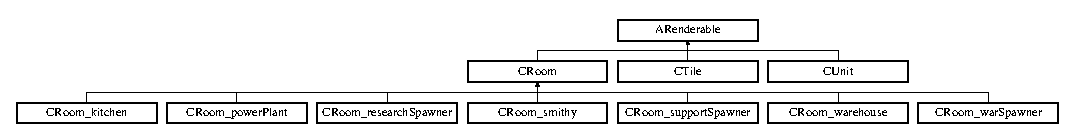
\includegraphics[height=1.428571cm]{classARenderable}
\end{center}
\end{figure}
\subsection*{Public Member Functions}
\begin{DoxyCompactItemize}
\item 
\hypertarget{classARenderable_a945fecfa1012fc94f186b8814f225ae8}{{\bfseries A\-Renderable} (\hyperlink{classCTexture}{C\-Texture} $\ast$p\-Texture, const \hyperlink{classsf_1_1Vector2}{sf\-::\-Vector2}$<$ int $>$ \&curr\-Sub)}\label{classARenderable_a945fecfa1012fc94f186b8814f225ae8}

\item 
\hypertarget{classARenderable_a3d575592900ff1796452f35e7c618e6d}{{\bfseries A\-Renderable} (\hyperlink{classCSprite}{C\-Sprite} $\ast$p\-Sprite)}\label{classARenderable_a3d575592900ff1796452f35e7c618e6d}

\item 
\hypertarget{classARenderable_a4dc17477a94447c2ece7c418a47e3860}{\hyperlink{classCSprite}{C\-Sprite} $\ast$const {\bfseries get\-Sprite} ()}\label{classARenderable_a4dc17477a94447c2ece7c418a47e3860}

\item 
\hypertarget{classARenderable_a2cbb5617817d6697fd817f87bceebf77}{\hyperlink{classsf_1_1Sprite}{sf\-::\-Sprite} $\ast$const {\bfseries get\-Sprite\-\_\-\-A\-P\-I} ()}\label{classARenderable_a2cbb5617817d6697fd817f87bceebf77}

\item 
\hypertarget{classARenderable_a77d3d8b9f8d7f0e8b860abba2f6c53c9}{\hyperlink{classsf_1_1Rect}{sf\-::\-Float\-Rect} {\bfseries get\-Global\-Bounds} ()}\label{classARenderable_a77d3d8b9f8d7f0e8b860abba2f6c53c9}

\item 
\hypertarget{classARenderable_a1d0db7e6ba2e9bf6d8accb4164531b46}{void {\bfseries set\-Position} (float x, float y)}\label{classARenderable_a1d0db7e6ba2e9bf6d8accb4164531b46}

\end{DoxyCompactItemize}
\subsection*{Protected Attributes}
\begin{DoxyCompactItemize}
\item 
\hypertarget{classARenderable_a6030df923c81b400e94ff1f6a9df41f8}{\hyperlink{classCSprite}{C\-Sprite} $\ast$ {\bfseries m\-\_\-p\-Sprite}}\label{classARenderable_a6030df923c81b400e94ff1f6a9df41f8}

\end{DoxyCompactItemize}


\subsection{Detailed Description}


Definition at line 15 of file A\-Renderable.\-h.



The documentation for this class was generated from the following files\-:\begin{DoxyCompactItemize}
\item 
/home/z\-Zelman/\-Dropbox/\-Placeholder-\/\-R\-T\-S/src/\-Abstracts/A\-Renderable.\-h\item 
/home/z\-Zelman/\-Dropbox/\-Placeholder-\/\-R\-T\-S/src/\-Abstracts/A\-Renderable.\-cpp\end{DoxyCompactItemize}

\hypertarget{classrapidxml_1_1attribute__iterator}{\section{rapidxml\-:\-:attribute\-\_\-iterator$<$ Ch $>$ Class Template Reference}
\label{classrapidxml_1_1attribute__iterator}\index{rapidxml\-::attribute\-\_\-iterator$<$ Ch $>$@{rapidxml\-::attribute\-\_\-iterator$<$ Ch $>$}}
}


Iterator of child attributes of \hyperlink{classrapidxml_1_1xml__node}{xml\-\_\-node}.  




{\ttfamily \#include $<$rapidxml\-\_\-iterators.\-hpp$>$}

\subsection*{Public Types}
\begin{DoxyCompactItemize}
\item 
\hypertarget{classrapidxml_1_1attribute__iterator_ad4280d358828ad9c3eb1a787decb162e}{typedef \hyperlink{classrapidxml_1_1xml__attribute}{xml\-\_\-attribute}$<$ Ch $>$ {\bfseries value\-\_\-type}}\label{classrapidxml_1_1attribute__iterator_ad4280d358828ad9c3eb1a787decb162e}

\item 
\hypertarget{classrapidxml_1_1attribute__iterator_a097343e44557de14de86b470d3f917d9}{typedef \hyperlink{classrapidxml_1_1xml__attribute}{xml\-\_\-attribute}$<$ Ch $>$ \& {\bfseries reference}}\label{classrapidxml_1_1attribute__iterator_a097343e44557de14de86b470d3f917d9}

\item 
\hypertarget{classrapidxml_1_1attribute__iterator_a69acc2e60270d6a062c03c9cb1cf2aa7}{typedef \hyperlink{classrapidxml_1_1xml__attribute}{xml\-\_\-attribute}$<$ Ch $>$ $\ast$ {\bfseries pointer}}\label{classrapidxml_1_1attribute__iterator_a69acc2e60270d6a062c03c9cb1cf2aa7}

\item 
\hypertarget{classrapidxml_1_1attribute__iterator_accfd6d8527d32b427496b42f71a2e37a}{typedef std\-::ptrdiff\-\_\-t {\bfseries difference\-\_\-type}}\label{classrapidxml_1_1attribute__iterator_accfd6d8527d32b427496b42f71a2e37a}

\item 
\hypertarget{classrapidxml_1_1attribute__iterator_a97ac5d8b98f5b03c68cc566f5ac0a9e0}{typedef \\*
std\-::bidirectional\-\_\-iterator\-\_\-tag {\bfseries iterator\-\_\-category}}\label{classrapidxml_1_1attribute__iterator_a97ac5d8b98f5b03c68cc566f5ac0a9e0}

\end{DoxyCompactItemize}
\subsection*{Public Member Functions}
\begin{DoxyCompactItemize}
\item 
\hypertarget{classrapidxml_1_1attribute__iterator_a1109344dead88533ae4dd68cea5d9613}{{\bfseries attribute\-\_\-iterator} (\hyperlink{classrapidxml_1_1xml__node}{xml\-\_\-node}$<$ Ch $>$ $\ast$node)}\label{classrapidxml_1_1attribute__iterator_a1109344dead88533ae4dd68cea5d9613}

\item 
\hypertarget{classrapidxml_1_1attribute__iterator_a5d8616bdd2d41119e2f342d77b4f56f9}{\hyperlink{classrapidxml_1_1xml__attribute}{reference} {\bfseries operator$\ast$} () const }\label{classrapidxml_1_1attribute__iterator_a5d8616bdd2d41119e2f342d77b4f56f9}

\item 
\hypertarget{classrapidxml_1_1attribute__iterator_a0975adffe3d178c0ac83652b9ab78791}{\hyperlink{classrapidxml_1_1xml__attribute}{pointer} {\bfseries operator-\/$>$} () const }\label{classrapidxml_1_1attribute__iterator_a0975adffe3d178c0ac83652b9ab78791}

\item 
\hypertarget{classrapidxml_1_1attribute__iterator_afe7d15a4a1b228f97f1d4ebd4f3f6cca}{\hyperlink{classrapidxml_1_1attribute__iterator}{attribute\-\_\-iterator} \& {\bfseries operator++} ()}\label{classrapidxml_1_1attribute__iterator_afe7d15a4a1b228f97f1d4ebd4f3f6cca}

\item 
\hypertarget{classrapidxml_1_1attribute__iterator_a82c8859b9eebd45caa3afc25b9e78c36}{\hyperlink{classrapidxml_1_1attribute__iterator}{attribute\-\_\-iterator} {\bfseries operator++} (int)}\label{classrapidxml_1_1attribute__iterator_a82c8859b9eebd45caa3afc25b9e78c36}

\item 
\hypertarget{classrapidxml_1_1attribute__iterator_af22f1ad3c11d3269b43b49e29b89d7d1}{\hyperlink{classrapidxml_1_1attribute__iterator}{attribute\-\_\-iterator} \& {\bfseries operator-\/-\/} ()}\label{classrapidxml_1_1attribute__iterator_af22f1ad3c11d3269b43b49e29b89d7d1}

\item 
\hypertarget{classrapidxml_1_1attribute__iterator_af52a8562ab1b2c0391cdde79f55e4a6f}{\hyperlink{classrapidxml_1_1attribute__iterator}{attribute\-\_\-iterator} {\bfseries operator-\/-\/} (int)}\label{classrapidxml_1_1attribute__iterator_af52a8562ab1b2c0391cdde79f55e4a6f}

\item 
\hypertarget{classrapidxml_1_1attribute__iterator_ab1dc8dd11d21e145a4e3f76d46aead0d}{bool {\bfseries operator==} (const \hyperlink{classrapidxml_1_1attribute__iterator}{attribute\-\_\-iterator}$<$ Ch $>$ \&rhs)}\label{classrapidxml_1_1attribute__iterator_ab1dc8dd11d21e145a4e3f76d46aead0d}

\item 
\hypertarget{classrapidxml_1_1attribute__iterator_a39e8cf336c324521fd9c720abf280d88}{bool {\bfseries operator!=} (const \hyperlink{classrapidxml_1_1attribute__iterator}{attribute\-\_\-iterator}$<$ Ch $>$ \&rhs)}\label{classrapidxml_1_1attribute__iterator_a39e8cf336c324521fd9c720abf280d88}

\end{DoxyCompactItemize}


\subsection{Detailed Description}
\subsubsection*{template$<$class Ch$>$class rapidxml\-::attribute\-\_\-iterator$<$ Ch $>$}

Iterator of child attributes of \hyperlink{classrapidxml_1_1xml__node}{xml\-\_\-node}. 

Definition at line 95 of file rapidxml\-\_\-iterators.\-hpp.



The documentation for this class was generated from the following file\-:\begin{DoxyCompactItemize}
\item 
/home/z\-Zelman/\-Dropbox/\-Placeholder-\/\-R\-T\-S/rapidxml-\/1.\-13/\hyperlink{rapidxml__iterators_8hpp}{rapidxml\-\_\-iterators.\-hpp}\end{DoxyCompactItemize}

\hypertarget{classAUpdate}{\section{A\-Update Class Reference}
\label{classAUpdate}\index{A\-Update@{A\-Update}}
}
Inheritance diagram for A\-Update\-:\begin{figure}[H]
\begin{center}
\leavevmode
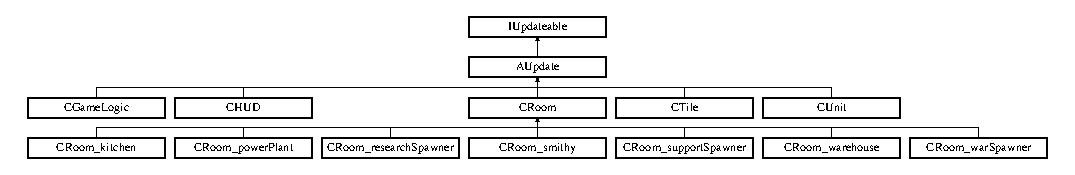
\includegraphics[height=1.904762cm]{classAUpdate}
\end{center}
\end{figure}
\subsection*{Public Member Functions}
\begin{DoxyCompactItemize}
\item 
\hypertarget{classAUpdate_a9f5be387e467fc5eea7fc45882abd949}{virtual void {\bfseries update} ()=0}\label{classAUpdate_a9f5be387e467fc5eea7fc45882abd949}

\end{DoxyCompactItemize}
\subsection*{Protected Attributes}
\begin{DoxyCompactItemize}
\item 
\hypertarget{classAUpdate_adf0a017c2fd5abd12f64f7f0fd992e66}{bool {\bfseries m\-\_\-is\-First\-Update}}\label{classAUpdate_adf0a017c2fd5abd12f64f7f0fd992e66}

\end{DoxyCompactItemize}


\subsection{Detailed Description}


Definition at line 13 of file A\-Update.\-h.



The documentation for this class was generated from the following files\-:\begin{DoxyCompactItemize}
\item 
/home/z\-Zelman/\-Dropbox/\-Placeholder-\/\-R\-T\-S/src/\-Abstracts/A\-Update.\-h\item 
/home/z\-Zelman/\-Dropbox/\-Placeholder-\/\-R\-T\-S/src/\-Abstracts/A\-Update.\-cpp\end{DoxyCompactItemize}

\hypertarget{classAUserInput}{\section{A\-User\-Input Class Reference}
\label{classAUserInput}\index{A\-User\-Input@{A\-User\-Input}}
}
Inheritance diagram for A\-User\-Input\-:\begin{figure}[H]
\begin{center}
\leavevmode
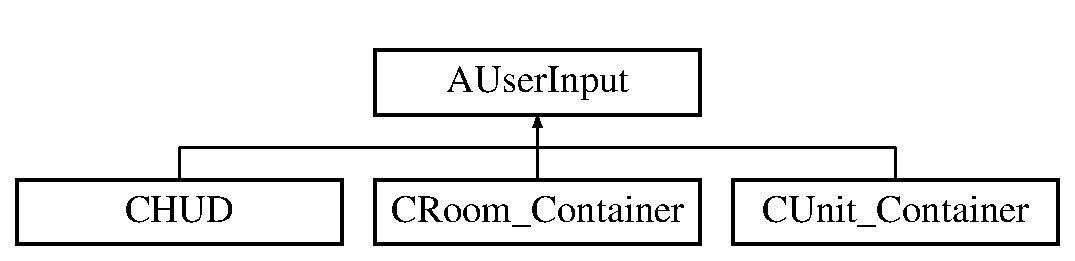
\includegraphics[height=2.000000cm]{classAUserInput}
\end{center}
\end{figure}
\subsection*{Classes}
\begin{DoxyCompactItemize}
\item 
struct \hyperlink{structAUserInput_1_1SKeyStates}{S\-Key\-States}
\end{DoxyCompactItemize}
\subsection*{Public Member Functions}
\begin{DoxyCompactItemize}
\item 
\hypertarget{classAUserInput_a110239bcc0461666583d1dc940cb5d13}{virtual bool {\bfseries user\-Input\-\_\-key\-Press} (\hyperlink{classsf_1_1Event}{sf\-::\-Event} $\ast$p\-Event)=0}\label{classAUserInput_a110239bcc0461666583d1dc940cb5d13}

\item 
\hypertarget{classAUserInput_afe8ae22fff673d788e366b9b29ffa67d}{virtual bool {\bfseries user\-Input\-\_\-key\-Release} (\hyperlink{classsf_1_1Event}{sf\-::\-Event} $\ast$p\-Event)=0}\label{classAUserInput_afe8ae22fff673d788e366b9b29ffa67d}

\item 
\hypertarget{classAUserInput_a567e0d0610bd2ef2e23fed64b3e56d2b}{virtual bool {\bfseries user\-Input\-\_\-mouse\-Press} (\hyperlink{classsf_1_1Event}{sf\-::\-Event} $\ast$p\-Event)=0}\label{classAUserInput_a567e0d0610bd2ef2e23fed64b3e56d2b}

\item 
\hypertarget{classAUserInput_a570f71dde4825c3e9bdcf6b58857f514}{virtual bool {\bfseries user\-Input\-\_\-mouse\-Release} (\hyperlink{classsf_1_1Event}{sf\-::\-Event} $\ast$p\-Event)=0}\label{classAUserInput_a570f71dde4825c3e9bdcf6b58857f514}

\end{DoxyCompactItemize}
\subsection*{Protected Attributes}
\begin{DoxyCompactItemize}
\item 
\hypertarget{classAUserInput_a55b881326b920413bbcdf6e02c4fb021}{struct \hyperlink{structAUserInput_1_1SKeyStates}{A\-User\-Input\-::\-S\-Key\-States} {\bfseries m\-\_\-s\-Keys}}\label{classAUserInput_a55b881326b920413bbcdf6e02c4fb021}

\end{DoxyCompactItemize}


\subsection{Detailed Description}


Definition at line 13 of file A\-User\-Input.\-h.



The documentation for this class was generated from the following files\-:\begin{DoxyCompactItemize}
\item 
/home/z\-Zelman/\-Dropbox/\-Placeholder-\/\-R\-T\-S/src/\-Abstracts/A\-User\-Input.\-h\item 
/home/z\-Zelman/\-Dropbox/\-Placeholder-\/\-R\-T\-S/src/\-Abstracts/A\-User\-Input.\-cpp\end{DoxyCompactItemize}

\hypertarget{classCGame}{\section{C\-Game Class Reference}
\label{classCGame}\index{C\-Game@{C\-Game}}
}
Inheritance diagram for C\-Game\-:\begin{figure}[H]
\begin{center}
\leavevmode
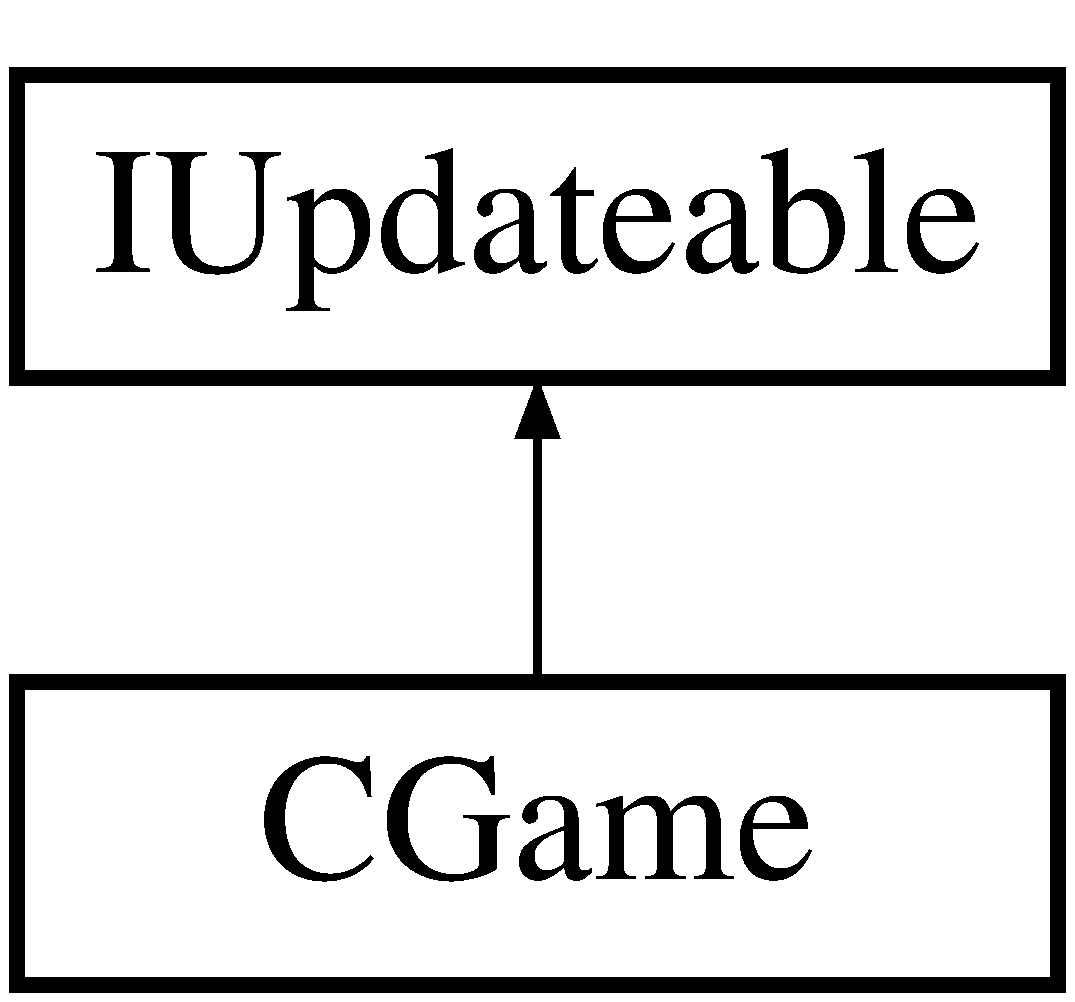
\includegraphics[height=2.000000cm]{classCGame}
\end{center}
\end{figure}
\subsection*{Public Member Functions}
\begin{DoxyCompactItemize}
\item 
\hypertarget{classCGame_a9ed0bb7ef800bc7e568cf8858c3b96ec}{\hyperlink{classsf_1_1RenderWindow}{sf\-::\-Render\-Window} $\ast$ {\bfseries get\-Game\-Window} ()}\label{classCGame_a9ed0bb7ef800bc7e568cf8858c3b96ec}

\item 
\hypertarget{classCGame_ae45938d7b77b13d2e80e4f9b3a17a44a}{bool {\bfseries get\-Is\-Running} ()}\label{classCGame_ae45938d7b77b13d2e80e4f9b3a17a44a}

\item 
\hypertarget{classCGame_a9b2f241693b1f024c957f92069fe6ed7}{bool {\bfseries get\-Is\-Paused} ()}\label{classCGame_a9b2f241693b1f024c957f92069fe6ed7}

\item 
\hypertarget{classCGame_aa94f04e2c012603f10430a4d4db3ce27}{void {\bfseries start\-Game} ()}\label{classCGame_aa94f04e2c012603f10430a4d4db3ce27}

\item 
\hypertarget{classCGame_acbad86ee58748e2db0da540f4aa0640e}{void {\bfseries stop\-Game} ()}\label{classCGame_acbad86ee58748e2db0da540f4aa0640e}

\end{DoxyCompactItemize}


\subsection{Detailed Description}


Definition at line 23 of file C\-Game.\-h.



The documentation for this class was generated from the following files\-:\begin{DoxyCompactItemize}
\item 
/home/z\-Zelman/\-Dropbox/\-Placeholder-\/\-R\-T\-S/src/C\-Game.\-h\item 
/home/z\-Zelman/\-Dropbox/\-Placeholder-\/\-R\-T\-S/src/C\-Game.\-cpp\end{DoxyCompactItemize}

\hypertarget{classCGameLogic}{\section{C\-Game\-Logic Class Reference}
\label{classCGameLogic}\index{C\-Game\-Logic@{C\-Game\-Logic}}
}
Inheritance diagram for C\-Game\-Logic\-:\begin{figure}[H]
\begin{center}
\leavevmode
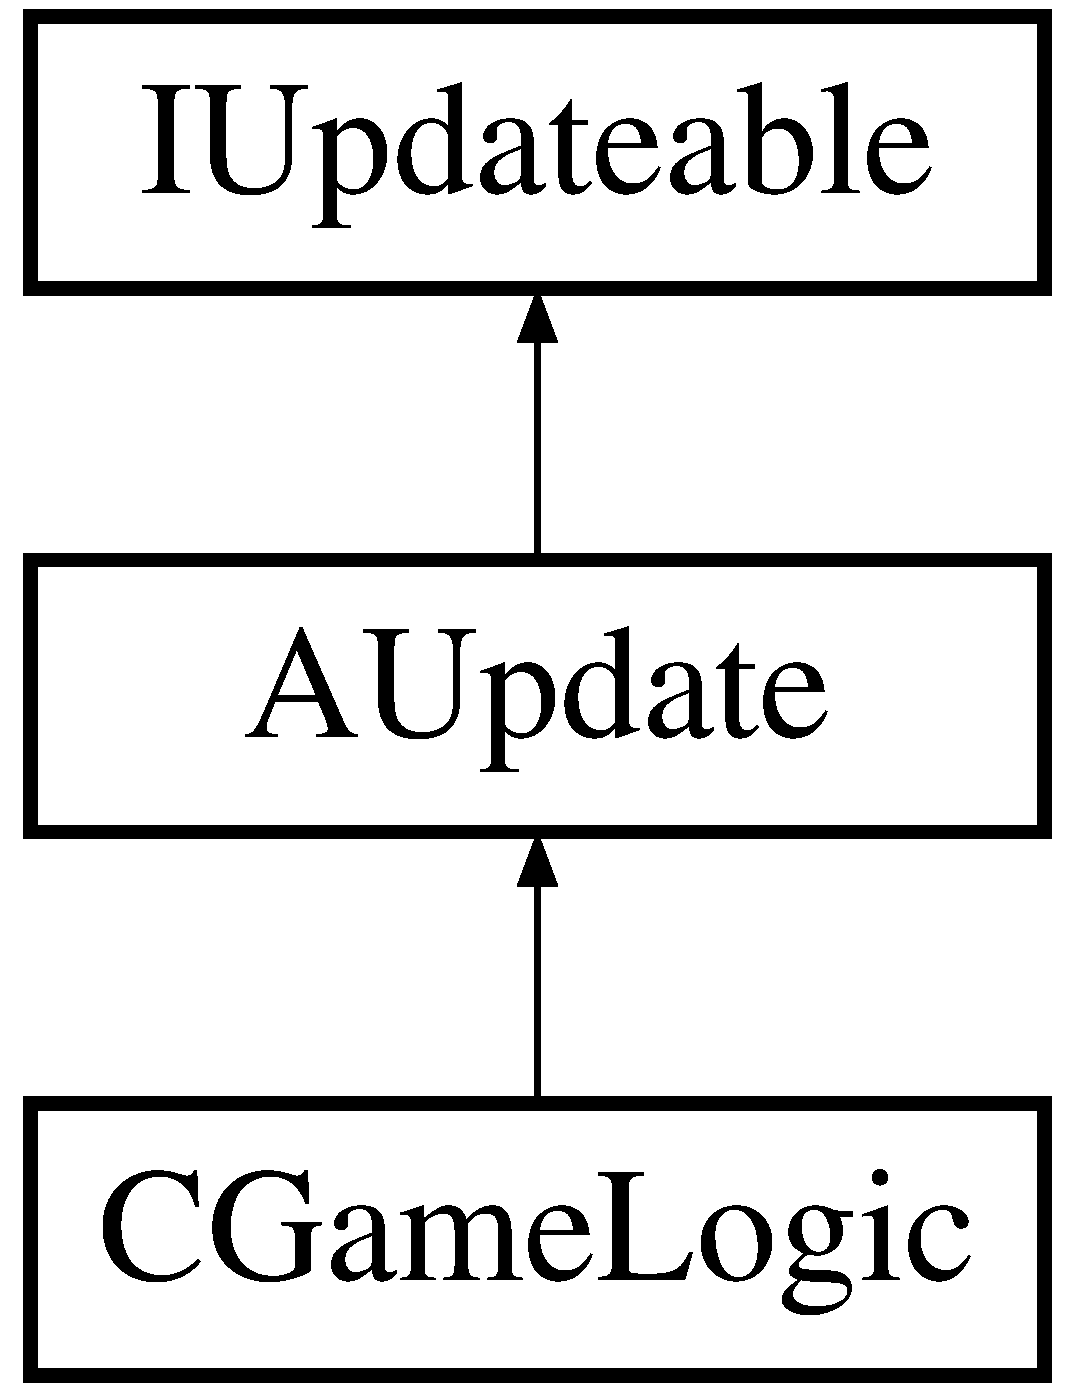
\includegraphics[height=3.000000cm]{classCGameLogic}
\end{center}
\end{figure}
\subsection*{Public Member Functions}
\begin{DoxyCompactItemize}
\item 
\hypertarget{classCGameLogic_ab32667a8e03199478e0170aad2cbd5f1}{{\bfseries C\-Game\-Logic} (\hyperlink{classCRoom__Container}{C\-Room\-\_\-\-Container} $\ast$p\-Room\-\_\-\-Container)}\label{classCGameLogic_ab32667a8e03199478e0170aad2cbd5f1}

\item 
\hypertarget{classCGameLogic_aa55d46e82f4a6e51de3dbb234d2ab940}{const \hyperlink{structSResources}{S\-Resources} $\ast$ {\bfseries get\-Resources} () const }\label{classCGameLogic_aa55d46e82f4a6e51de3dbb234d2ab940}

\item 
\hypertarget{classCGameLogic_a21e8fcd8ef9898522118ff66b8f13739}{void {\bfseries update} ()}\label{classCGameLogic_a21e8fcd8ef9898522118ff66b8f13739}

\end{DoxyCompactItemize}
\subsection*{Additional Inherited Members}


\subsection{Detailed Description}


Definition at line 33 of file C\-Game\-Logic.\-h.



The documentation for this class was generated from the following files\-:\begin{DoxyCompactItemize}
\item 
/home/z\-Zelman/\-Dropbox/\-Placeholder-\/\-R\-T\-S/src/\-Logic/C\-Game\-Logic.\-h\item 
/home/z\-Zelman/\-Dropbox/\-Placeholder-\/\-R\-T\-S/src/\-Logic/C\-Game\-Logic.\-cpp\end{DoxyCompactItemize}

\hypertarget{classCHUD}{\section{C\-H\-U\-D Class Reference}
\label{classCHUD}\index{C\-H\-U\-D@{C\-H\-U\-D}}
}
Inheritance diagram for C\-H\-U\-D\-:\begin{figure}[H]
\begin{center}
\leavevmode
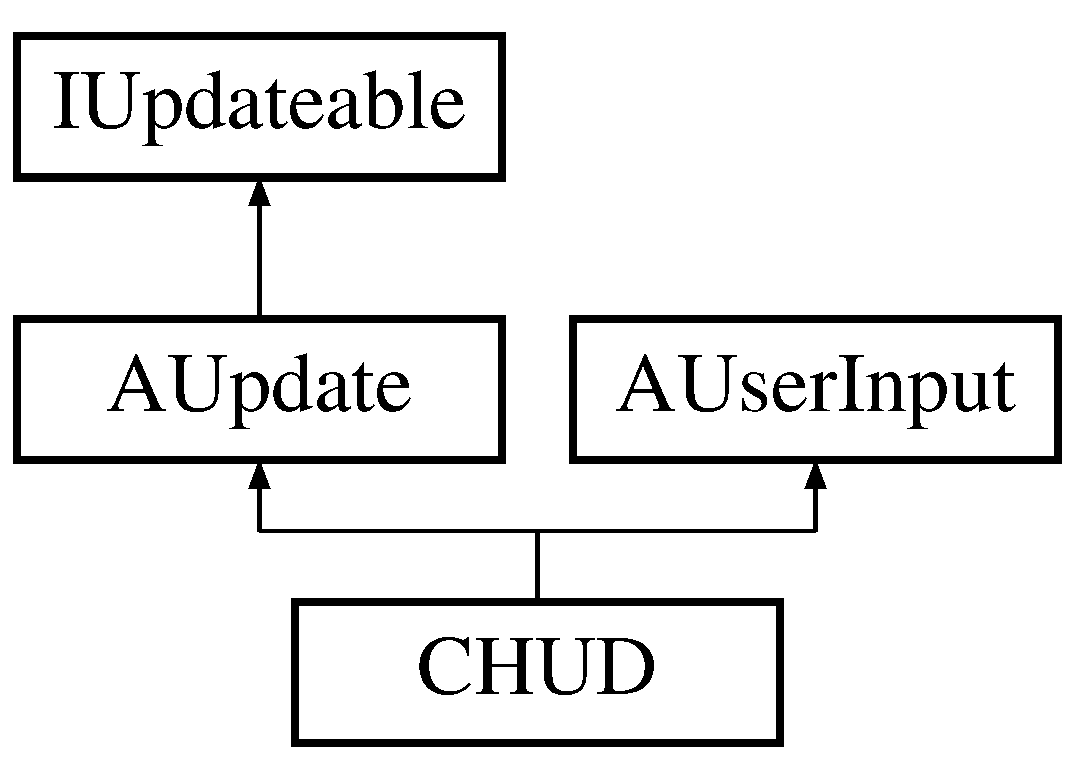
\includegraphics[height=3.000000cm]{classCHUD}
\end{center}
\end{figure}
\subsection*{Public Member Functions}
\begin{DoxyCompactItemize}
\item 
\hypertarget{classCHUD_ab519309240f9a867ac92d973cbeca0a5}{{\bfseries C\-H\-U\-D} (\hyperlink{classsf_1_1RenderWindow}{sf\-::\-Render\-Window} $\ast$p\-Window, \hyperlink{classCGameLogic}{C\-Game\-Logic} $\ast$p\-Game\-Logic)}\label{classCHUD_ab519309240f9a867ac92d973cbeca0a5}

\item 
\hypertarget{classCHUD_a992f78972db3fc54681ba720f3a08e9a}{void {\bfseries render} ()}\label{classCHUD_a992f78972db3fc54681ba720f3a08e9a}

\item 
\hypertarget{classCHUD_a598ee42887c834e6f6ffaf8d4be0723d}{void {\bfseries update} ()}\label{classCHUD_a598ee42887c834e6f6ffaf8d4be0723d}

\item 
\hypertarget{classCHUD_af2fb4b789ebabd8e12109c599f6039ea}{bool {\bfseries user\-Input\-\_\-key\-Press} (\hyperlink{classsf_1_1Event}{sf\-::\-Event} $\ast$p\-Event)}\label{classCHUD_af2fb4b789ebabd8e12109c599f6039ea}

\item 
\hypertarget{classCHUD_a229ff3daa4c721dfd72d12b94e43e89f}{bool {\bfseries user\-Input\-\_\-key\-Release} (\hyperlink{classsf_1_1Event}{sf\-::\-Event} $\ast$p\-Event)}\label{classCHUD_a229ff3daa4c721dfd72d12b94e43e89f}

\item 
\hypertarget{classCHUD_a592852471c152a8eeb4321250e4b5818}{bool {\bfseries user\-Input\-\_\-mouse\-Press} (\hyperlink{classsf_1_1Event}{sf\-::\-Event} $\ast$p\-Event)}\label{classCHUD_a592852471c152a8eeb4321250e4b5818}

\item 
\hypertarget{classCHUD_ad48f5d418a93d0e5767e6b95cc834827}{bool {\bfseries user\-Input\-\_\-mouse\-Release} (\hyperlink{classsf_1_1Event}{sf\-::\-Event} $\ast$p\-Event)}\label{classCHUD_ad48f5d418a93d0e5767e6b95cc834827}

\end{DoxyCompactItemize}
\subsection*{Additional Inherited Members}


\subsection{Detailed Description}


Definition at line 21 of file C\-H\-U\-D.\-h.



The documentation for this class was generated from the following files\-:\begin{DoxyCompactItemize}
\item 
/home/z\-Zelman/\-Dropbox/\-Placeholder-\/\-R\-T\-S/src/\-H\-U\-D/C\-H\-U\-D.\-h\item 
/home/z\-Zelman/\-Dropbox/\-Placeholder-\/\-R\-T\-S/src/\-H\-U\-D/C\-H\-U\-D.\-cpp\end{DoxyCompactItemize}

\hypertarget{structsf_1_1SoundStream_1_1Chunk}{\section{sf\-:\-:Sound\-Stream\-:\-:Chunk Struct Reference}
\label{structsf_1_1SoundStream_1_1Chunk}\index{sf\-::\-Sound\-Stream\-::\-Chunk@{sf\-::\-Sound\-Stream\-::\-Chunk}}
}


Structure defining a chunk of audio data to stream.  




{\ttfamily \#include $<$Sound\-Stream.\-hpp$>$}

\subsection*{Public Attributes}
\begin{DoxyCompactItemize}
\item 
\hypertarget{structsf_1_1SoundStream_1_1Chunk_aa3b84d69adbe663a17a7671626076df4}{const Int16 $\ast$ \hyperlink{structsf_1_1SoundStream_1_1Chunk_aa3b84d69adbe663a17a7671626076df4}{samples}}\label{structsf_1_1SoundStream_1_1Chunk_aa3b84d69adbe663a17a7671626076df4}

\begin{DoxyCompactList}\small\item\em Pointer to the audio samples. \end{DoxyCompactList}\item 
\hypertarget{structsf_1_1SoundStream_1_1Chunk_af47f5d94012acf8b11f056ba77aff97a}{std\-::size\-\_\-t \hyperlink{structsf_1_1SoundStream_1_1Chunk_af47f5d94012acf8b11f056ba77aff97a}{sample\-Count}}\label{structsf_1_1SoundStream_1_1Chunk_af47f5d94012acf8b11f056ba77aff97a}

\begin{DoxyCompactList}\small\item\em Number of samples pointed by Samples. \end{DoxyCompactList}\end{DoxyCompactItemize}


\subsection{Detailed Description}
Structure defining a chunk of audio data to stream. 

Definition at line 52 of file Sound\-Stream.\-hpp.



The documentation for this struct was generated from the following file\-:\begin{DoxyCompactItemize}
\item 
/home/z\-Zelman/\-Dropbox/\-Placeholder-\/\-R\-T\-S/\-S\-F\-M\-L-\/2.\-1/include/\-S\-F\-M\-L/\-Audio/Sound\-Stream.\-hpp\end{DoxyCompactItemize}

\hypertarget{classsf_1_1CircleShape}{\section{sf\-:\-:Circle\-Shape Class Reference}
\label{classsf_1_1CircleShape}\index{sf\-::\-Circle\-Shape@{sf\-::\-Circle\-Shape}}
}


Specialized shape representing a circle.  




{\ttfamily \#include $<$Circle\-Shape.\-hpp$>$}

Inheritance diagram for sf\-:\-:Circle\-Shape\-:\begin{figure}[H]
\begin{center}
\leavevmode
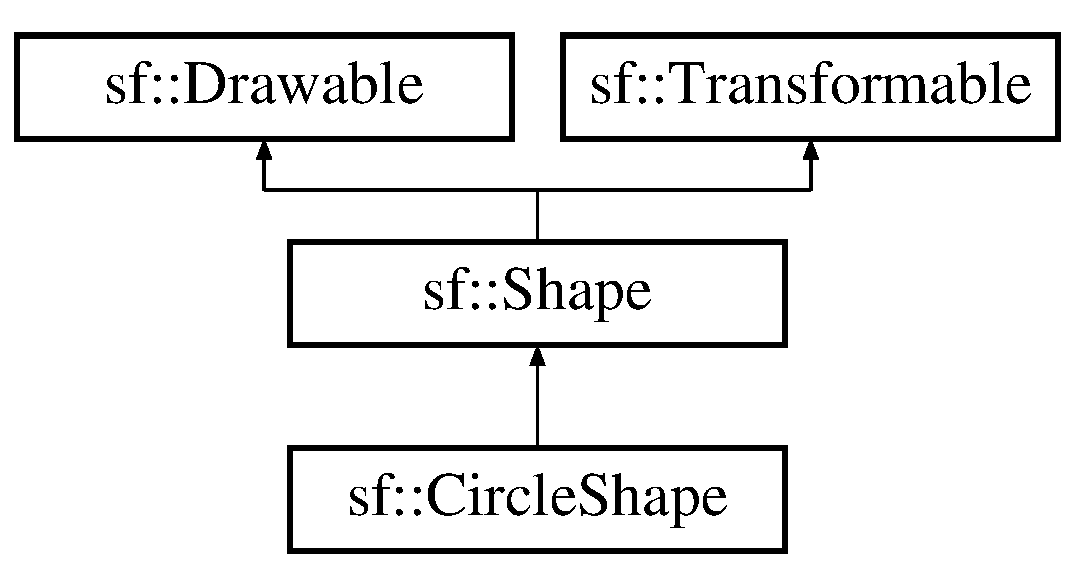
\includegraphics[height=3.000000cm]{classsf_1_1CircleShape}
\end{center}
\end{figure}
\subsection*{Public Member Functions}
\begin{DoxyCompactItemize}
\item 
\hyperlink{classsf_1_1CircleShape_a06a5e136da1cfa3bd2a945a5c7f718d3}{Circle\-Shape} (float radius=0, unsigned int point\-Count=30)
\begin{DoxyCompactList}\small\item\em Default constructor. \end{DoxyCompactList}\item 
void \hyperlink{classsf_1_1CircleShape_a21cdf85fc2f201e10222a241af864be0}{set\-Radius} (float radius)
\begin{DoxyCompactList}\small\item\em Set the radius of the circle. \end{DoxyCompactList}\item 
float \hyperlink{classsf_1_1CircleShape_afaf5175a75b6179cc177b1281027ab00}{get\-Radius} () const 
\begin{DoxyCompactList}\small\item\em Get the radius of the circle. \end{DoxyCompactList}\item 
void \hyperlink{classsf_1_1CircleShape_a84249c4b23b20c24bf6891edde3cf744}{set\-Point\-Count} (unsigned int count)
\begin{DoxyCompactList}\small\item\em Set the number of points of the circle. \end{DoxyCompactList}\item 
virtual unsigned int \hyperlink{classsf_1_1CircleShape_ae41ed830ca8f459e88ea6f125c240949}{get\-Point\-Count} () const 
\begin{DoxyCompactList}\small\item\em Get the number of points of the shape. \end{DoxyCompactList}\item 
virtual \hyperlink{classsf_1_1Vector2}{Vector2f} \hyperlink{classsf_1_1CircleShape_a05139deaef220ed3d5a3bc4ca9aa9dbe}{get\-Point} (unsigned int index) const 
\begin{DoxyCompactList}\small\item\em Get a point of the shape. \end{DoxyCompactList}\end{DoxyCompactItemize}
\subsection*{Additional Inherited Members}


\subsection{Detailed Description}
Specialized shape representing a circle. 

This class inherits all the functions of \hyperlink{classsf_1_1Transformable}{sf\-::\-Transformable} (position, rotation, scale, bounds, ...) as well as the functions of \hyperlink{classsf_1_1Shape}{sf\-::\-Shape} (outline, color, texture, ...).

Usage example\-: 
\begin{DoxyCode}
\hyperlink{classsf_1_1CircleShape}{sf::CircleShape} circle;
circle.\hyperlink{classsf_1_1CircleShape_a21cdf85fc2f201e10222a241af864be0}{setRadius}(150);
circle.\hyperlink{classsf_1_1Shape_a5978f41ee349ac3c52942996dcb184f7}{setOutlineColor}(\hyperlink{classsf_1_1Color_a127dbf55db9c07d0fa8f4bfcbb97594a}{sf::Color::Red});
circle.\hyperlink{classsf_1_1Shape_a5ad336ad74fc1f567fce3b7e44cf87dc}{setOutlineThickness}(5);
circle.\hyperlink{classsf_1_1Transformable_a4dbfb1a7c80688b0b4c477d706550208}{setPosition}(10, 20);
...
window.draw(circle);
\end{DoxyCode}


Since the graphics card can't draw perfect circles, we have to fake them with multiple triangles connected to each other. The \char`\"{}points count\char`\"{} property of \hyperlink{classsf_1_1CircleShape}{sf\-::\-Circle\-Shape} defines how many of these triangles to use, and therefore defines the quality of the circle.

The number of points can also be used for another purpose; with small numbers you can create any regular polygon shape\-: equilateral triangle, square, pentagon, hexagon, ...

\begin{DoxySeeAlso}{See Also}
\hyperlink{classsf_1_1Shape}{sf\-::\-Shape}, \hyperlink{classsf_1_1RectangleShape}{sf\-::\-Rectangle\-Shape}, \hyperlink{classsf_1_1ConvexShape}{sf\-::\-Convex\-Shape} 
\end{DoxySeeAlso}


Definition at line 41 of file Circle\-Shape.\-hpp.



\subsection{Constructor \& Destructor Documentation}
\hypertarget{classsf_1_1CircleShape_a06a5e136da1cfa3bd2a945a5c7f718d3}{\index{sf\-::\-Circle\-Shape@{sf\-::\-Circle\-Shape}!Circle\-Shape@{Circle\-Shape}}
\index{Circle\-Shape@{Circle\-Shape}!sf::CircleShape@{sf\-::\-Circle\-Shape}}
\subsubsection[{Circle\-Shape}]{\setlength{\rightskip}{0pt plus 5cm}sf\-::\-Circle\-Shape\-::\-Circle\-Shape (
\begin{DoxyParamCaption}
\item[{float}]{radius = {\ttfamily 0}, }
\item[{unsigned int}]{point\-Count = {\ttfamily 30}}
\end{DoxyParamCaption}
)\hspace{0.3cm}{\ttfamily [explicit]}}}\label{classsf_1_1CircleShape_a06a5e136da1cfa3bd2a945a5c7f718d3}


Default constructor. 


\begin{DoxyParams}{Parameters}
{\em radius} & Radius of the circle \\
\hline
{\em point\-Count} & Number of points composing the circle \\
\hline
\end{DoxyParams}


\subsection{Member Function Documentation}
\hypertarget{classsf_1_1CircleShape_a05139deaef220ed3d5a3bc4ca9aa9dbe}{\index{sf\-::\-Circle\-Shape@{sf\-::\-Circle\-Shape}!get\-Point@{get\-Point}}
\index{get\-Point@{get\-Point}!sf::CircleShape@{sf\-::\-Circle\-Shape}}
\subsubsection[{get\-Point}]{\setlength{\rightskip}{0pt plus 5cm}virtual {\bf Vector2f} sf\-::\-Circle\-Shape\-::get\-Point (
\begin{DoxyParamCaption}
\item[{unsigned int}]{index}
\end{DoxyParamCaption}
) const\hspace{0.3cm}{\ttfamily [virtual]}}}\label{classsf_1_1CircleShape_a05139deaef220ed3d5a3bc4ca9aa9dbe}


Get a point of the shape. 

The result is undefined if {\itshape index} is out of the valid range.


\begin{DoxyParams}{Parameters}
{\em index} & Index of the point to get, in range \mbox{[}0 .. \hyperlink{classsf_1_1CircleShape_ae41ed830ca8f459e88ea6f125c240949}{get\-Point\-Count()} -\/ 1\mbox{]}\\
\hline
\end{DoxyParams}
\begin{DoxyReturn}{Returns}
Index-\/th point of the shape 
\end{DoxyReturn}


Implements \hyperlink{classsf_1_1Shape_a397f3b4cdb7ad98cdc6c034816c652d2}{sf\-::\-Shape}.

\hypertarget{classsf_1_1CircleShape_ae41ed830ca8f459e88ea6f125c240949}{\index{sf\-::\-Circle\-Shape@{sf\-::\-Circle\-Shape}!get\-Point\-Count@{get\-Point\-Count}}
\index{get\-Point\-Count@{get\-Point\-Count}!sf::CircleShape@{sf\-::\-Circle\-Shape}}
\subsubsection[{get\-Point\-Count}]{\setlength{\rightskip}{0pt plus 5cm}virtual unsigned int sf\-::\-Circle\-Shape\-::get\-Point\-Count (
\begin{DoxyParamCaption}
{}
\end{DoxyParamCaption}
) const\hspace{0.3cm}{\ttfamily [virtual]}}}\label{classsf_1_1CircleShape_ae41ed830ca8f459e88ea6f125c240949}


Get the number of points of the shape. 

\begin{DoxyReturn}{Returns}
Number of points of the shape
\end{DoxyReturn}
\begin{DoxySeeAlso}{See Also}
\hyperlink{classsf_1_1CircleShape_a84249c4b23b20c24bf6891edde3cf744}{set\-Point\-Count} 
\end{DoxySeeAlso}


Implements \hyperlink{classsf_1_1Shape_ad84e1b675ecd270ad8151aea4e271a78}{sf\-::\-Shape}.

\hypertarget{classsf_1_1CircleShape_afaf5175a75b6179cc177b1281027ab00}{\index{sf\-::\-Circle\-Shape@{sf\-::\-Circle\-Shape}!get\-Radius@{get\-Radius}}
\index{get\-Radius@{get\-Radius}!sf::CircleShape@{sf\-::\-Circle\-Shape}}
\subsubsection[{get\-Radius}]{\setlength{\rightskip}{0pt plus 5cm}float sf\-::\-Circle\-Shape\-::get\-Radius (
\begin{DoxyParamCaption}
{}
\end{DoxyParamCaption}
) const}}\label{classsf_1_1CircleShape_afaf5175a75b6179cc177b1281027ab00}


Get the radius of the circle. 

\begin{DoxyReturn}{Returns}
Radius of the circle
\end{DoxyReturn}
\begin{DoxySeeAlso}{See Also}
\hyperlink{classsf_1_1CircleShape_a21cdf85fc2f201e10222a241af864be0}{set\-Radius} 
\end{DoxySeeAlso}
\hypertarget{classsf_1_1CircleShape_a84249c4b23b20c24bf6891edde3cf744}{\index{sf\-::\-Circle\-Shape@{sf\-::\-Circle\-Shape}!set\-Point\-Count@{set\-Point\-Count}}
\index{set\-Point\-Count@{set\-Point\-Count}!sf::CircleShape@{sf\-::\-Circle\-Shape}}
\subsubsection[{set\-Point\-Count}]{\setlength{\rightskip}{0pt plus 5cm}void sf\-::\-Circle\-Shape\-::set\-Point\-Count (
\begin{DoxyParamCaption}
\item[{unsigned int}]{count}
\end{DoxyParamCaption}
)}}\label{classsf_1_1CircleShape_a84249c4b23b20c24bf6891edde3cf744}


Set the number of points of the circle. 


\begin{DoxyParams}{Parameters}
{\em count} & New number of points of the circle\\
\hline
\end{DoxyParams}
\begin{DoxySeeAlso}{See Also}
\hyperlink{classsf_1_1CircleShape_ae41ed830ca8f459e88ea6f125c240949}{get\-Point\-Count} 
\end{DoxySeeAlso}
\hypertarget{classsf_1_1CircleShape_a21cdf85fc2f201e10222a241af864be0}{\index{sf\-::\-Circle\-Shape@{sf\-::\-Circle\-Shape}!set\-Radius@{set\-Radius}}
\index{set\-Radius@{set\-Radius}!sf::CircleShape@{sf\-::\-Circle\-Shape}}
\subsubsection[{set\-Radius}]{\setlength{\rightskip}{0pt plus 5cm}void sf\-::\-Circle\-Shape\-::set\-Radius (
\begin{DoxyParamCaption}
\item[{float}]{radius}
\end{DoxyParamCaption}
)}}\label{classsf_1_1CircleShape_a21cdf85fc2f201e10222a241af864be0}


Set the radius of the circle. 


\begin{DoxyParams}{Parameters}
{\em radius} & New radius of the circle\\
\hline
\end{DoxyParams}
\begin{DoxySeeAlso}{See Also}
\hyperlink{classsf_1_1CircleShape_afaf5175a75b6179cc177b1281027ab00}{get\-Radius} 
\end{DoxySeeAlso}


The documentation for this class was generated from the following file\-:\begin{DoxyCompactItemize}
\item 
/home/z\-Zelman/\-Dropbox/\-Placeholder-\/\-R\-T\-S/\-S\-F\-M\-L-\/2.\-1/include/\-S\-F\-M\-L/\-Graphics/Circle\-Shape.\-hpp\end{DoxyCompactItemize}

\hypertarget{classsf_1_1Clock}{\section{sf\-:\-:Clock Class Reference}
\label{classsf_1_1Clock}\index{sf\-::\-Clock@{sf\-::\-Clock}}
}


Utility class that measures the elapsed time.  




{\ttfamily \#include $<$Clock.\-hpp$>$}

\subsection*{Public Member Functions}
\begin{DoxyCompactItemize}
\item 
\hyperlink{classsf_1_1Clock_abbc959c7830ca7c3a4da133cb506d3fd}{Clock} ()
\begin{DoxyCompactList}\small\item\em Default constructor. \end{DoxyCompactList}\item 
\hyperlink{classsf_1_1Time}{Time} \hyperlink{classsf_1_1Clock_a799feb6acb099b57b58d8d20984fce11}{get\-Elapsed\-Time} () const 
\begin{DoxyCompactList}\small\item\em Get the elapsed time. \end{DoxyCompactList}\item 
\hyperlink{classsf_1_1Time}{Time} \hyperlink{classsf_1_1Clock_a123e2627f2943e5ecaa1db0c7df3231b}{restart} ()
\begin{DoxyCompactList}\small\item\em Restart the clock. \end{DoxyCompactList}\end{DoxyCompactItemize}


\subsection{Detailed Description}
Utility class that measures the elapsed time. 

\hyperlink{classsf_1_1Clock}{sf\-::\-Clock} is a lightweight class for measuring time.

Its provides the most precise time that the underlying O\-S can achieve (generally microseconds or nanoseconds). It also ensures monotonicity, which means that the returned time can never go backward, even if the system time is changed.

Usage example\-: 
\begin{DoxyCode}
\hyperlink{classsf_1_1Clock}{sf::Clock} clock;
...
Time time1 = clock.\hyperlink{classsf_1_1Clock_a799feb6acb099b57b58d8d20984fce11}{getElapsedTime}();
...
\hyperlink{classsf_1_1Time_acba0cfbc49e3a09a22a8e079eb67a05c}{Time} time2 = clock.\hyperlink{classsf_1_1Clock_a123e2627f2943e5ecaa1db0c7df3231b}{restart}();
\end{DoxyCode}


The \hyperlink{classsf_1_1Time}{sf\-::\-Time} value returned by the clock can then be converted to a number of seconds, milliseconds or even microseconds.

\begin{DoxySeeAlso}{See Also}
\hyperlink{classsf_1_1Time}{sf\-::\-Time} 
\end{DoxySeeAlso}


Definition at line 41 of file Clock.\-hpp.



\subsection{Constructor \& Destructor Documentation}
\hypertarget{classsf_1_1Clock_abbc959c7830ca7c3a4da133cb506d3fd}{\index{sf\-::\-Clock@{sf\-::\-Clock}!Clock@{Clock}}
\index{Clock@{Clock}!sf::Clock@{sf\-::\-Clock}}
\subsubsection[{Clock}]{\setlength{\rightskip}{0pt plus 5cm}sf\-::\-Clock\-::\-Clock (
\begin{DoxyParamCaption}
{}
\end{DoxyParamCaption}
)}}\label{classsf_1_1Clock_abbc959c7830ca7c3a4da133cb506d3fd}


Default constructor. 

The clock starts automatically after being constructed. 

\subsection{Member Function Documentation}
\hypertarget{classsf_1_1Clock_a799feb6acb099b57b58d8d20984fce11}{\index{sf\-::\-Clock@{sf\-::\-Clock}!get\-Elapsed\-Time@{get\-Elapsed\-Time}}
\index{get\-Elapsed\-Time@{get\-Elapsed\-Time}!sf::Clock@{sf\-::\-Clock}}
\subsubsection[{get\-Elapsed\-Time}]{\setlength{\rightskip}{0pt plus 5cm}{\bf Time} sf\-::\-Clock\-::get\-Elapsed\-Time (
\begin{DoxyParamCaption}
{}
\end{DoxyParamCaption}
) const}}\label{classsf_1_1Clock_a799feb6acb099b57b58d8d20984fce11}


Get the elapsed time. 

This function returns the time elapsed since the last call to \hyperlink{classsf_1_1Clock_a123e2627f2943e5ecaa1db0c7df3231b}{restart()} (or the construction of the instance if \hyperlink{classsf_1_1Clock_a123e2627f2943e5ecaa1db0c7df3231b}{restart()} has not been called).

\begin{DoxyReturn}{Returns}
\hyperlink{classsf_1_1Time}{Time} elapsed 
\end{DoxyReturn}
\hypertarget{classsf_1_1Clock_a123e2627f2943e5ecaa1db0c7df3231b}{\index{sf\-::\-Clock@{sf\-::\-Clock}!restart@{restart}}
\index{restart@{restart}!sf::Clock@{sf\-::\-Clock}}
\subsubsection[{restart}]{\setlength{\rightskip}{0pt plus 5cm}{\bf Time} sf\-::\-Clock\-::restart (
\begin{DoxyParamCaption}
{}
\end{DoxyParamCaption}
)}}\label{classsf_1_1Clock_a123e2627f2943e5ecaa1db0c7df3231b}


Restart the clock. 

This function puts the time counter back to zero. It also returns the time elapsed since the clock was started.

\begin{DoxyReturn}{Returns}
\hyperlink{classsf_1_1Time}{Time} elapsed 
\end{DoxyReturn}


The documentation for this class was generated from the following file\-:\begin{DoxyCompactItemize}
\item 
/home/z\-Zelman/\-Dropbox/\-Placeholder-\/\-R\-T\-S/\-S\-F\-M\-L-\/2.\-1/include/\-S\-F\-M\-L/\-System/Clock.\-hpp\end{DoxyCompactItemize}

\hypertarget{classsf_1_1Color}{\section{sf\-:\-:Color Class Reference}
\label{classsf_1_1Color}\index{sf\-::\-Color@{sf\-::\-Color}}
}


Utility class for manpulating R\-G\-B\-A colors.  




{\ttfamily \#include $<$Color.\-hpp$>$}

\subsection*{Public Member Functions}
\begin{DoxyCompactItemize}
\item 
\hyperlink{classsf_1_1Color_ac2eb4393fb11ad3fa3ccf34e92fe08e4}{Color} ()
\begin{DoxyCompactList}\small\item\em Default constructor. \end{DoxyCompactList}\item 
\hyperlink{classsf_1_1Color_ac791dc61be4c60baac50fe700f1c9850}{Color} (Uint8 red, Uint8 green, Uint8 blue, Uint8 alpha=255)
\begin{DoxyCompactList}\small\item\em Construct the color from its 4 R\-G\-B\-A components. \end{DoxyCompactList}\end{DoxyCompactItemize}
\subsection*{Public Attributes}
\begin{DoxyCompactItemize}
\item 
\hypertarget{classsf_1_1Color_a6a5256ca24a4f9f0e0808f6fc23e01e1}{Uint8 \hyperlink{classsf_1_1Color_a6a5256ca24a4f9f0e0808f6fc23e01e1}{r}}\label{classsf_1_1Color_a6a5256ca24a4f9f0e0808f6fc23e01e1}

\begin{DoxyCompactList}\small\item\em Red component. \end{DoxyCompactList}\item 
\hypertarget{classsf_1_1Color_a591daf9c3c55dea830c76c962d6ba1a5}{Uint8 \hyperlink{classsf_1_1Color_a591daf9c3c55dea830c76c962d6ba1a5}{g}}\label{classsf_1_1Color_a591daf9c3c55dea830c76c962d6ba1a5}

\begin{DoxyCompactList}\small\item\em Green component. \end{DoxyCompactList}\item 
\hypertarget{classsf_1_1Color_a6707aedd0609c8920e12df5d7abc53cb}{Uint8 \hyperlink{classsf_1_1Color_a6707aedd0609c8920e12df5d7abc53cb}{b}}\label{classsf_1_1Color_a6707aedd0609c8920e12df5d7abc53cb}

\begin{DoxyCompactList}\small\item\em Blue component. \end{DoxyCompactList}\item 
\hypertarget{classsf_1_1Color_a56dbdb47d5f040d9b78ac6a0b8b3a831}{Uint8 \hyperlink{classsf_1_1Color_a56dbdb47d5f040d9b78ac6a0b8b3a831}{a}}\label{classsf_1_1Color_a56dbdb47d5f040d9b78ac6a0b8b3a831}

\begin{DoxyCompactList}\small\item\em Alpha (opacity) component. \end{DoxyCompactList}\end{DoxyCompactItemize}
\subsection*{Static Public Attributes}
\begin{DoxyCompactItemize}
\item 
\hypertarget{classsf_1_1Color_a77c688197b981338f0b19dc58bd2facd}{static const \hyperlink{classsf_1_1Color}{Color} \hyperlink{classsf_1_1Color_a77c688197b981338f0b19dc58bd2facd}{Black}}\label{classsf_1_1Color_a77c688197b981338f0b19dc58bd2facd}

\begin{DoxyCompactList}\small\item\em Black predefined color. \end{DoxyCompactList}\item 
\hypertarget{classsf_1_1Color_a4fd874712178d9e206f53226002aa4ca}{static const \hyperlink{classsf_1_1Color}{Color} \hyperlink{classsf_1_1Color_a4fd874712178d9e206f53226002aa4ca}{White}}\label{classsf_1_1Color_a4fd874712178d9e206f53226002aa4ca}

\begin{DoxyCompactList}\small\item\em White predefined color. \end{DoxyCompactList}\item 
\hypertarget{classsf_1_1Color_a127dbf55db9c07d0fa8f4bfcbb97594a}{static const \hyperlink{classsf_1_1Color}{Color} \hyperlink{classsf_1_1Color_a127dbf55db9c07d0fa8f4bfcbb97594a}{Red}}\label{classsf_1_1Color_a127dbf55db9c07d0fa8f4bfcbb97594a}

\begin{DoxyCompactList}\small\item\em Red predefined color. \end{DoxyCompactList}\item 
\hypertarget{classsf_1_1Color_a95629b30de8c6856aa7d3afed12eb865}{static const \hyperlink{classsf_1_1Color}{Color} \hyperlink{classsf_1_1Color_a95629b30de8c6856aa7d3afed12eb865}{Green}}\label{classsf_1_1Color_a95629b30de8c6856aa7d3afed12eb865}

\begin{DoxyCompactList}\small\item\em Green predefined color. \end{DoxyCompactList}\item 
\hypertarget{classsf_1_1Color_ab03770d4817426b2614cfc33cf0e245c}{static const \hyperlink{classsf_1_1Color}{Color} \hyperlink{classsf_1_1Color_ab03770d4817426b2614cfc33cf0e245c}{Blue}}\label{classsf_1_1Color_ab03770d4817426b2614cfc33cf0e245c}

\begin{DoxyCompactList}\small\item\em Blue predefined color. \end{DoxyCompactList}\item 
\hypertarget{classsf_1_1Color_af8896b5f56650935f5b9d72d528802c7}{static const \hyperlink{classsf_1_1Color}{Color} \hyperlink{classsf_1_1Color_af8896b5f56650935f5b9d72d528802c7}{Yellow}}\label{classsf_1_1Color_af8896b5f56650935f5b9d72d528802c7}

\begin{DoxyCompactList}\small\item\em Yellow predefined color. \end{DoxyCompactList}\item 
\hypertarget{classsf_1_1Color_a6fe70d90b65b2163dd066a84ac00426c}{static const \hyperlink{classsf_1_1Color}{Color} \hyperlink{classsf_1_1Color_a6fe70d90b65b2163dd066a84ac00426c}{Magenta}}\label{classsf_1_1Color_a6fe70d90b65b2163dd066a84ac00426c}

\begin{DoxyCompactList}\small\item\em Magenta predefined color. \end{DoxyCompactList}\item 
\hypertarget{classsf_1_1Color_a64ae9beb0b9a5865dd811cda4bb18340}{static const \hyperlink{classsf_1_1Color}{Color} \hyperlink{classsf_1_1Color_a64ae9beb0b9a5865dd811cda4bb18340}{Cyan}}\label{classsf_1_1Color_a64ae9beb0b9a5865dd811cda4bb18340}

\begin{DoxyCompactList}\small\item\em Cyan predefined color. \end{DoxyCompactList}\item 
\hypertarget{classsf_1_1Color_a569b45471737f770656f50ae7bbac292}{static const \hyperlink{classsf_1_1Color}{Color} \hyperlink{classsf_1_1Color_a569b45471737f770656f50ae7bbac292}{Transparent}}\label{classsf_1_1Color_a569b45471737f770656f50ae7bbac292}

\begin{DoxyCompactList}\small\item\em Transparent (black) predefined color. \end{DoxyCompactList}\end{DoxyCompactItemize}
\subsection*{Related Functions}
(Note that these are not member functions.) \begin{DoxyCompactItemize}
\item 
S\-F\-M\-L\-\_\-\-G\-R\-A\-P\-H\-I\-C\-S\-\_\-\-A\-P\-I bool \hyperlink{classsf_1_1Color_a7498d4670c7655e8d4d91ef49cc6064e}{operator==} (const \hyperlink{classsf_1_1Color}{Color} \&left, const \hyperlink{classsf_1_1Color}{Color} \&right)
\begin{DoxyCompactList}\small\item\em Overload of the == operator. \end{DoxyCompactList}\item 
S\-F\-M\-L\-\_\-\-G\-R\-A\-P\-H\-I\-C\-S\-\_\-\-A\-P\-I bool \hyperlink{classsf_1_1Color_a5d6501b7dd05f481b79f7163899f1d92}{operator!=} (const \hyperlink{classsf_1_1Color}{Color} \&left, const \hyperlink{classsf_1_1Color}{Color} \&right)
\begin{DoxyCompactList}\small\item\em Overload of the != operator. \end{DoxyCompactList}\item 
S\-F\-M\-L\-\_\-\-G\-R\-A\-P\-H\-I\-C\-S\-\_\-\-A\-P\-I \hyperlink{classsf_1_1Color}{Color} \hyperlink{classsf_1_1Color_a90e79ecc276114cda519a88119ac645b}{operator+} (const \hyperlink{classsf_1_1Color}{Color} \&left, const \hyperlink{classsf_1_1Color}{Color} \&right)
\begin{DoxyCompactList}\small\item\em Overload of the binary + operator. \end{DoxyCompactList}\item 
S\-F\-M\-L\-\_\-\-G\-R\-A\-P\-H\-I\-C\-S\-\_\-\-A\-P\-I \hyperlink{classsf_1_1Color}{Color} \hyperlink{classsf_1_1Color_aa9de267d831b4ec8ba65b627e51d50c3}{operator$\ast$} (const \hyperlink{classsf_1_1Color}{Color} \&left, const \hyperlink{classsf_1_1Color}{Color} \&right)
\begin{DoxyCompactList}\small\item\em Overload of the binary $\ast$ operator. \end{DoxyCompactList}\item 
S\-F\-M\-L\-\_\-\-G\-R\-A\-P\-H\-I\-C\-S\-\_\-\-A\-P\-I \hyperlink{classsf_1_1Color}{Color} \& \hyperlink{classsf_1_1Color_a19917f2453a4acfd69de2539bfab8031}{operator+=} (\hyperlink{classsf_1_1Color}{Color} \&left, const \hyperlink{classsf_1_1Color}{Color} \&right)
\begin{DoxyCompactList}\small\item\em Overload of the binary += operator. \end{DoxyCompactList}\item 
S\-F\-M\-L\-\_\-\-G\-R\-A\-P\-H\-I\-C\-S\-\_\-\-A\-P\-I \hyperlink{classsf_1_1Color}{Color} \& \hyperlink{classsf_1_1Color_a8953be58a47ced92fb25966d6ee90511}{operator$\ast$=} (\hyperlink{classsf_1_1Color}{Color} \&left, const \hyperlink{classsf_1_1Color}{Color} \&right)
\begin{DoxyCompactList}\small\item\em Overload of the binary $\ast$= operator. \end{DoxyCompactList}\end{DoxyCompactItemize}


\subsection{Detailed Description}
Utility class for manpulating R\-G\-B\-A colors. 

\hyperlink{classsf_1_1Color}{sf\-::\-Color} is a simple color class composed of 4 components\-: \begin{DoxyItemize}
\item Red \item Green \item Blue \item Alpha (opacity)\end{DoxyItemize}
Each component is a public member, an unsigned integer in the range \mbox{[}0, 255\mbox{]}. Thus, colors can be constructed and manipulated very easily\-:


\begin{DoxyCode}
\hyperlink{classsf_1_1Color}{sf::Color} color(255, 0, 0); \textcolor{comment}{// red}
color.r = 0;                \textcolor{comment}{// make it black}
color.b = 128;              \textcolor{comment}{// make it dark blue}
\end{DoxyCode}


The fourth component of colors, named \char`\"{}alpha\char`\"{}, represents the opacity of the color. A color with an alpha value of 255 will be fully opaque, while an alpha value of 0 will make a color fully transparent, whatever the value of the other components is.

The most common colors are already defined as static variables\-: 
\begin{DoxyCode}
\hyperlink{classsf_1_1Color}{sf::Color} black       = \hyperlink{classsf_1_1Color_a77c688197b981338f0b19dc58bd2facd}{sf::Color::Black};
\hyperlink{classsf_1_1Color}{sf::Color} white       = \hyperlink{classsf_1_1Color_a4fd874712178d9e206f53226002aa4ca}{sf::Color::White};
\hyperlink{classsf_1_1Color}{sf::Color} red         = \hyperlink{classsf_1_1Color_a127dbf55db9c07d0fa8f4bfcbb97594a}{sf::Color::Red};
\hyperlink{classsf_1_1Color}{sf::Color} green       = \hyperlink{classsf_1_1Color_a95629b30de8c6856aa7d3afed12eb865}{sf::Color::Green};
\hyperlink{classsf_1_1Color}{sf::Color} blue        = \hyperlink{classsf_1_1Color_ab03770d4817426b2614cfc33cf0e245c}{sf::Color::Blue};
\hyperlink{classsf_1_1Color}{sf::Color} yellow      = \hyperlink{classsf_1_1Color_af8896b5f56650935f5b9d72d528802c7}{sf::Color::Yellow};
\hyperlink{classsf_1_1Color}{sf::Color} magenta     = \hyperlink{classsf_1_1Color_a6fe70d90b65b2163dd066a84ac00426c}{sf::Color::Magenta};
\hyperlink{classsf_1_1Color}{sf::Color} cyan        = \hyperlink{classsf_1_1Color_a64ae9beb0b9a5865dd811cda4bb18340}{sf::Color::Cyan};
\hyperlink{classsf_1_1Color}{sf::Color} transparent = \hyperlink{classsf_1_1Color_a569b45471737f770656f50ae7bbac292}{sf::Color::Transparent};
\end{DoxyCode}


Colors can also be added and modulated (multiplied) using the overloaded operators + and $\ast$. 

Definition at line 40 of file Color.\-hpp.



\subsection{Constructor \& Destructor Documentation}
\hypertarget{classsf_1_1Color_ac2eb4393fb11ad3fa3ccf34e92fe08e4}{\index{sf\-::\-Color@{sf\-::\-Color}!Color@{Color}}
\index{Color@{Color}!sf::Color@{sf\-::\-Color}}
\subsubsection[{Color}]{\setlength{\rightskip}{0pt plus 5cm}sf\-::\-Color\-::\-Color (
\begin{DoxyParamCaption}
{}
\end{DoxyParamCaption}
)}}\label{classsf_1_1Color_ac2eb4393fb11ad3fa3ccf34e92fe08e4}


Default constructor. 

Constructs an opaque black color. It is equivalent to \hyperlink{classsf_1_1Color}{sf\-::\-Color(0, 0, 0, 255)}. \hypertarget{classsf_1_1Color_ac791dc61be4c60baac50fe700f1c9850}{\index{sf\-::\-Color@{sf\-::\-Color}!Color@{Color}}
\index{Color@{Color}!sf::Color@{sf\-::\-Color}}
\subsubsection[{Color}]{\setlength{\rightskip}{0pt plus 5cm}sf\-::\-Color\-::\-Color (
\begin{DoxyParamCaption}
\item[{Uint8}]{red, }
\item[{Uint8}]{green, }
\item[{Uint8}]{blue, }
\item[{Uint8}]{alpha = {\ttfamily 255}}
\end{DoxyParamCaption}
)}}\label{classsf_1_1Color_ac791dc61be4c60baac50fe700f1c9850}


Construct the color from its 4 R\-G\-B\-A components. 


\begin{DoxyParams}{Parameters}
{\em red} & Red component (in the range \mbox{[}0, 255\mbox{]}) \\
\hline
{\em green} & Green component (in the range \mbox{[}0, 255\mbox{]}) \\
\hline
{\em blue} & Blue component (in the range \mbox{[}0, 255\mbox{]}) \\
\hline
{\em alpha} & Alpha (opacity) component (in the range \mbox{[}0, 255\mbox{]}) \\
\hline
\end{DoxyParams}


\subsection{Friends And Related Function Documentation}
\hypertarget{classsf_1_1Color_a5d6501b7dd05f481b79f7163899f1d92}{\index{sf\-::\-Color@{sf\-::\-Color}!operator!=@{operator!=}}
\index{operator!=@{operator!=}!sf::Color@{sf\-::\-Color}}
\subsubsection[{operator!=}]{\setlength{\rightskip}{0pt plus 5cm}S\-F\-M\-L\-\_\-\-G\-R\-A\-P\-H\-I\-C\-S\-\_\-\-A\-P\-I bool operator!= (
\begin{DoxyParamCaption}
\item[{const {\bf Color} \&}]{left, }
\item[{const {\bf Color} \&}]{right}
\end{DoxyParamCaption}
)\hspace{0.3cm}{\ttfamily [related]}}}\label{classsf_1_1Color_a5d6501b7dd05f481b79f7163899f1d92}


Overload of the != operator. 

This operator compares two colors and check if they are different.


\begin{DoxyParams}{Parameters}
{\em left} & Left operand \\
\hline
{\em right} & Right operand\\
\hline
\end{DoxyParams}
\begin{DoxyReturn}{Returns}
True if colors are different, false if they are equal 
\end{DoxyReturn}
\hypertarget{classsf_1_1Color_aa9de267d831b4ec8ba65b627e51d50c3}{\index{sf\-::\-Color@{sf\-::\-Color}!operator$\ast$@{operator$\ast$}}
\index{operator$\ast$@{operator$\ast$}!sf::Color@{sf\-::\-Color}}
\subsubsection[{operator$\ast$}]{\setlength{\rightskip}{0pt plus 5cm}S\-F\-M\-L\-\_\-\-G\-R\-A\-P\-H\-I\-C\-S\-\_\-\-A\-P\-I {\bf Color} operator$\ast$ (
\begin{DoxyParamCaption}
\item[{const {\bf Color} \&}]{left, }
\item[{const {\bf Color} \&}]{right}
\end{DoxyParamCaption}
)\hspace{0.3cm}{\ttfamily [related]}}}\label{classsf_1_1Color_aa9de267d831b4ec8ba65b627e51d50c3}


Overload of the binary $\ast$ operator. 

This operator returns the component-\/wise multiplication (also called \char`\"{}modulation\char`\"{}) of two colors. Components are then divided by 255 so that the result is still in the range \mbox{[}0, 255\mbox{]}.


\begin{DoxyParams}{Parameters}
{\em left} & Left operand \\
\hline
{\em right} & Right operand\\
\hline
\end{DoxyParams}
\begin{DoxyReturn}{Returns}
Result of {\itshape left} $\ast$ {\itshape right} 
\end{DoxyReturn}
\hypertarget{classsf_1_1Color_a8953be58a47ced92fb25966d6ee90511}{\index{sf\-::\-Color@{sf\-::\-Color}!operator$\ast$=@{operator$\ast$=}}
\index{operator$\ast$=@{operator$\ast$=}!sf::Color@{sf\-::\-Color}}
\subsubsection[{operator$\ast$=}]{\setlength{\rightskip}{0pt plus 5cm}S\-F\-M\-L\-\_\-\-G\-R\-A\-P\-H\-I\-C\-S\-\_\-\-A\-P\-I {\bf Color} \& operator$\ast$= (
\begin{DoxyParamCaption}
\item[{{\bf Color} \&}]{left, }
\item[{const {\bf Color} \&}]{right}
\end{DoxyParamCaption}
)\hspace{0.3cm}{\ttfamily [related]}}}\label{classsf_1_1Color_a8953be58a47ced92fb25966d6ee90511}


Overload of the binary $\ast$= operator. 

This operator returns the component-\/wise multiplication (also called \char`\"{}modulation\char`\"{}) of two colors, and assigns the result to the left operand. Components are then divided by 255 so that the result is still in the range \mbox{[}0, 255\mbox{]}.


\begin{DoxyParams}{Parameters}
{\em left} & Left operand \\
\hline
{\em right} & Right operand\\
\hline
\end{DoxyParams}
\begin{DoxyReturn}{Returns}
Reference to {\itshape left} 
\end{DoxyReturn}
\hypertarget{classsf_1_1Color_a90e79ecc276114cda519a88119ac645b}{\index{sf\-::\-Color@{sf\-::\-Color}!operator+@{operator+}}
\index{operator+@{operator+}!sf::Color@{sf\-::\-Color}}
\subsubsection[{operator+}]{\setlength{\rightskip}{0pt plus 5cm}S\-F\-M\-L\-\_\-\-G\-R\-A\-P\-H\-I\-C\-S\-\_\-\-A\-P\-I {\bf Color} operator+ (
\begin{DoxyParamCaption}
\item[{const {\bf Color} \&}]{left, }
\item[{const {\bf Color} \&}]{right}
\end{DoxyParamCaption}
)\hspace{0.3cm}{\ttfamily [related]}}}\label{classsf_1_1Color_a90e79ecc276114cda519a88119ac645b}


Overload of the binary + operator. 

This operator returns the component-\/wise sum of two colors. Components that exceed 255 are clamped to 255.


\begin{DoxyParams}{Parameters}
{\em left} & Left operand \\
\hline
{\em right} & Right operand\\
\hline
\end{DoxyParams}
\begin{DoxyReturn}{Returns}
Result of {\itshape left} + {\itshape right} 
\end{DoxyReturn}
\hypertarget{classsf_1_1Color_a19917f2453a4acfd69de2539bfab8031}{\index{sf\-::\-Color@{sf\-::\-Color}!operator+=@{operator+=}}
\index{operator+=@{operator+=}!sf::Color@{sf\-::\-Color}}
\subsubsection[{operator+=}]{\setlength{\rightskip}{0pt plus 5cm}S\-F\-M\-L\-\_\-\-G\-R\-A\-P\-H\-I\-C\-S\-\_\-\-A\-P\-I {\bf Color} \& operator+= (
\begin{DoxyParamCaption}
\item[{{\bf Color} \&}]{left, }
\item[{const {\bf Color} \&}]{right}
\end{DoxyParamCaption}
)\hspace{0.3cm}{\ttfamily [related]}}}\label{classsf_1_1Color_a19917f2453a4acfd69de2539bfab8031}


Overload of the binary += operator. 

This operator computes the component-\/wise sum of two colors, and assigns the result to the left operand. Components that exceed 255 are clamped to 255.


\begin{DoxyParams}{Parameters}
{\em left} & Left operand \\
\hline
{\em right} & Right operand\\
\hline
\end{DoxyParams}
\begin{DoxyReturn}{Returns}
Reference to {\itshape left} 
\end{DoxyReturn}
\hypertarget{classsf_1_1Color_a7498d4670c7655e8d4d91ef49cc6064e}{\index{sf\-::\-Color@{sf\-::\-Color}!operator==@{operator==}}
\index{operator==@{operator==}!sf::Color@{sf\-::\-Color}}
\subsubsection[{operator==}]{\setlength{\rightskip}{0pt plus 5cm}S\-F\-M\-L\-\_\-\-G\-R\-A\-P\-H\-I\-C\-S\-\_\-\-A\-P\-I bool operator== (
\begin{DoxyParamCaption}
\item[{const {\bf Color} \&}]{left, }
\item[{const {\bf Color} \&}]{right}
\end{DoxyParamCaption}
)\hspace{0.3cm}{\ttfamily [related]}}}\label{classsf_1_1Color_a7498d4670c7655e8d4d91ef49cc6064e}


Overload of the == operator. 

This operator compares two colors and check if they are equal.


\begin{DoxyParams}{Parameters}
{\em left} & Left operand \\
\hline
{\em right} & Right operand\\
\hline
\end{DoxyParams}
\begin{DoxyReturn}{Returns}
True if colors are equal, false if they are different 
\end{DoxyReturn}


The documentation for this class was generated from the following file\-:\begin{DoxyCompactItemize}
\item 
/home/z\-Zelman/\-Dropbox/\-Placeholder-\/\-R\-T\-S/\-S\-F\-M\-L-\/2.\-1/include/\-S\-F\-M\-L/\-Graphics/Color.\-hpp\end{DoxyCompactItemize}

\hypertarget{classsf_1_1Context}{\section{sf\-:\-:Context Class Reference}
\label{classsf_1_1Context}\index{sf\-::\-Context@{sf\-::\-Context}}
}


Class holding a valid drawing context.  




{\ttfamily \#include $<$Context.\-hpp$>$}

Inheritance diagram for sf\-:\-:Context\-:\begin{figure}[H]
\begin{center}
\leavevmode
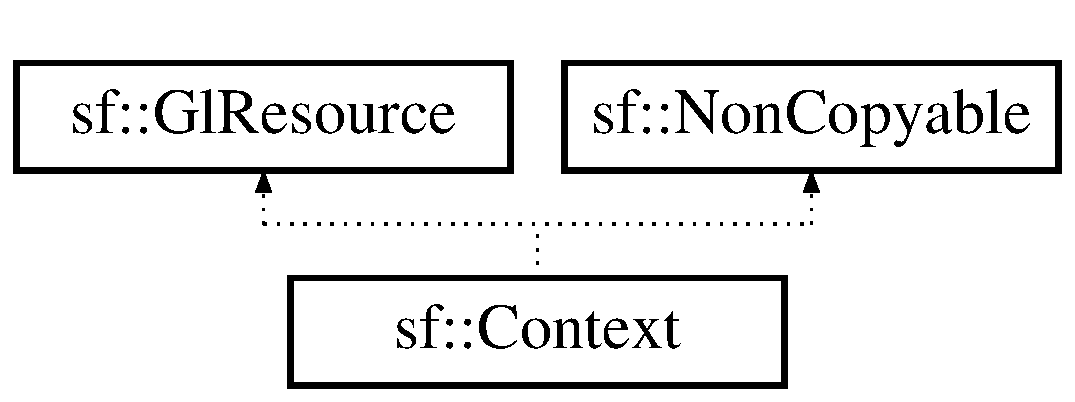
\includegraphics[height=2.000000cm]{classsf_1_1Context}
\end{center}
\end{figure}
\subsection*{Public Member Functions}
\begin{DoxyCompactItemize}
\item 
\hyperlink{classsf_1_1Context_aba22797a790706ca2c5c04ee39f2b555}{Context} ()
\begin{DoxyCompactList}\small\item\em Default constructor. \end{DoxyCompactList}\item 
\hyperlink{classsf_1_1Context_a805b1bbdb3e52b1fda7c9bf2cd6ca86b}{$\sim$\-Context} ()
\begin{DoxyCompactList}\small\item\em Destructor. \end{DoxyCompactList}\item 
bool \hyperlink{classsf_1_1Context_a0806f915ea81ae1f4e8135a7a3696562}{set\-Active} (bool active)
\begin{DoxyCompactList}\small\item\em Activate or deactivate explicitely the context. \end{DoxyCompactList}\item 
\hyperlink{classsf_1_1Context_a2a9e3529e48919120e6b6fc10bad296c}{Context} (const \hyperlink{structsf_1_1ContextSettings}{Context\-Settings} \&settings, unsigned int width, unsigned int height)
\begin{DoxyCompactList}\small\item\em Construct a in-\/memory context. \end{DoxyCompactList}\end{DoxyCompactItemize}


\subsection{Detailed Description}
Class holding a valid drawing context. 

If you need to make Open\-G\-L calls without having an active window (like in a thread), you can use an instance of this class to get a valid context.

Having a valid context is necessary for {\itshape every} Open\-G\-L call.

Note that a context is only active in its current thread, if you create a new thread it will have no valid context by default.

To use a \hyperlink{classsf_1_1Context}{sf\-::\-Context} instance, just construct it and let it live as long as you need a valid context. No explicit activation is needed, all it has to do is to exist. Its destructor will take care of deactivating and freeing all the attached resources.

Usage example\-: 
\begin{DoxyCode}
\textcolor{keywordtype}{void} threadFunction(\textcolor{keywordtype}{void}*)
\{
   \hyperlink{classsf_1_1Context}{sf::Context} context;
   \textcolor{comment}{// from now on, you have a valid context}

   \textcolor{comment}{// you can make OpenGL calls}
   glClear(GL\_DEPTH\_BUFFER\_BIT);
\}
\textcolor{comment}{// the context is automatically deactivated and destroyed}
\textcolor{comment}{// by the sf::Context destructor}
\end{DoxyCode}
 

Definition at line 48 of file Context.\-hpp.



\subsection{Constructor \& Destructor Documentation}
\hypertarget{classsf_1_1Context_aba22797a790706ca2c5c04ee39f2b555}{\index{sf\-::\-Context@{sf\-::\-Context}!Context@{Context}}
\index{Context@{Context}!sf::Context@{sf\-::\-Context}}
\subsubsection[{Context}]{\setlength{\rightskip}{0pt plus 5cm}sf\-::\-Context\-::\-Context (
\begin{DoxyParamCaption}
{}
\end{DoxyParamCaption}
)}}\label{classsf_1_1Context_aba22797a790706ca2c5c04ee39f2b555}


Default constructor. 

The constructor creates and activates the context \hypertarget{classsf_1_1Context_a805b1bbdb3e52b1fda7c9bf2cd6ca86b}{\index{sf\-::\-Context@{sf\-::\-Context}!$\sim$\-Context@{$\sim$\-Context}}
\index{$\sim$\-Context@{$\sim$\-Context}!sf::Context@{sf\-::\-Context}}
\subsubsection[{$\sim$\-Context}]{\setlength{\rightskip}{0pt plus 5cm}sf\-::\-Context\-::$\sim$\-Context (
\begin{DoxyParamCaption}
{}
\end{DoxyParamCaption}
)}}\label{classsf_1_1Context_a805b1bbdb3e52b1fda7c9bf2cd6ca86b}


Destructor. 

The desctructor deactivates and destroys the context \hypertarget{classsf_1_1Context_a2a9e3529e48919120e6b6fc10bad296c}{\index{sf\-::\-Context@{sf\-::\-Context}!Context@{Context}}
\index{Context@{Context}!sf::Context@{sf\-::\-Context}}
\subsubsection[{Context}]{\setlength{\rightskip}{0pt plus 5cm}sf\-::\-Context\-::\-Context (
\begin{DoxyParamCaption}
\item[{const {\bf Context\-Settings} \&}]{settings, }
\item[{unsigned int}]{width, }
\item[{unsigned int}]{height}
\end{DoxyParamCaption}
)}}\label{classsf_1_1Context_a2a9e3529e48919120e6b6fc10bad296c}


Construct a in-\/memory context. 

This constructor is for internal use, you don't need to bother with it.


\begin{DoxyParams}{Parameters}
{\em settings} & Creation parameters \\
\hline
{\em width} & Back buffer width \\
\hline
{\em height} & Back buffer height \\
\hline
\end{DoxyParams}


\subsection{Member Function Documentation}
\hypertarget{classsf_1_1Context_a0806f915ea81ae1f4e8135a7a3696562}{\index{sf\-::\-Context@{sf\-::\-Context}!set\-Active@{set\-Active}}
\index{set\-Active@{set\-Active}!sf::Context@{sf\-::\-Context}}
\subsubsection[{set\-Active}]{\setlength{\rightskip}{0pt plus 5cm}bool sf\-::\-Context\-::set\-Active (
\begin{DoxyParamCaption}
\item[{bool}]{active}
\end{DoxyParamCaption}
)}}\label{classsf_1_1Context_a0806f915ea81ae1f4e8135a7a3696562}


Activate or deactivate explicitely the context. 


\begin{DoxyParams}{Parameters}
{\em active} & True to activate, false to deactivate\\
\hline
\end{DoxyParams}
\begin{DoxyReturn}{Returns}
True on success, false on failure 
\end{DoxyReturn}


The documentation for this class was generated from the following file\-:\begin{DoxyCompactItemize}
\item 
/home/z\-Zelman/\-Dropbox/\-Placeholder-\/\-R\-T\-S/\-S\-F\-M\-L-\/2.\-1/include/\-S\-F\-M\-L/\-Window/Context.\-hpp\end{DoxyCompactItemize}

\hypertarget{structsf_1_1ContextSettings}{\section{sf\-:\-:Context\-Settings Class Reference}
\label{structsf_1_1ContextSettings}\index{sf\-::\-Context\-Settings@{sf\-::\-Context\-Settings}}
}


Structure defining the settings of the Open\-G\-L context attached to a window.  




{\ttfamily \#include $<$Context\-Settings.\-hpp$>$}

\subsection*{Public Member Functions}
\begin{DoxyCompactItemize}
\item 
\hyperlink{structsf_1_1ContextSettings_aafe35f8e257f9d1e496ed64e33e2ee9f}{Context\-Settings} (unsigned int depth=0, unsigned int stencil=0, unsigned int antialiasing=0, unsigned int major=2, unsigned int minor=0)
\begin{DoxyCompactList}\small\item\em Default constructor. \end{DoxyCompactList}\end{DoxyCompactItemize}
\subsection*{Public Attributes}
\begin{DoxyCompactItemize}
\item 
\hypertarget{structsf_1_1ContextSettings_a4809e22089c2af7276b8809b5aede7bb}{unsigned int \hyperlink{structsf_1_1ContextSettings_a4809e22089c2af7276b8809b5aede7bb}{depth\-Bits}}\label{structsf_1_1ContextSettings_a4809e22089c2af7276b8809b5aede7bb}

\begin{DoxyCompactList}\small\item\em Bits of the depth buffer. \end{DoxyCompactList}\item 
\hypertarget{structsf_1_1ContextSettings_ac2e788c201ca20e84fd38a28071abd29}{unsigned int \hyperlink{structsf_1_1ContextSettings_ac2e788c201ca20e84fd38a28071abd29}{stencil\-Bits}}\label{structsf_1_1ContextSettings_ac2e788c201ca20e84fd38a28071abd29}

\begin{DoxyCompactList}\small\item\em Bits of the stencil buffer. \end{DoxyCompactList}\item 
\hypertarget{structsf_1_1ContextSettings_ac4a097be18994dba38d73f36b0418bdc}{unsigned int \hyperlink{structsf_1_1ContextSettings_ac4a097be18994dba38d73f36b0418bdc}{antialiasing\-Level}}\label{structsf_1_1ContextSettings_ac4a097be18994dba38d73f36b0418bdc}

\begin{DoxyCompactList}\small\item\em Level of antialiasing. \end{DoxyCompactList}\item 
\hypertarget{structsf_1_1ContextSettings_a99a680d5c15a7e34c935654155dd5166}{unsigned int \hyperlink{structsf_1_1ContextSettings_a99a680d5c15a7e34c935654155dd5166}{major\-Version}}\label{structsf_1_1ContextSettings_a99a680d5c15a7e34c935654155dd5166}

\begin{DoxyCompactList}\small\item\em Major number of the context version to create. \end{DoxyCompactList}\item 
\hypertarget{structsf_1_1ContextSettings_aaeb0efe9d2658b840da93b30554b100f}{unsigned int \hyperlink{structsf_1_1ContextSettings_aaeb0efe9d2658b840da93b30554b100f}{minor\-Version}}\label{structsf_1_1ContextSettings_aaeb0efe9d2658b840da93b30554b100f}

\begin{DoxyCompactList}\small\item\em Minor number of the context version to create. \end{DoxyCompactList}\end{DoxyCompactItemize}


\subsection{Detailed Description}
Structure defining the settings of the Open\-G\-L context attached to a window. 

\hyperlink{structsf_1_1ContextSettings}{Context\-Settings} allows to define several advanced settings of the Open\-G\-L context attached to a window. All these settings have no impact on the regular S\-F\-M\-L rendering (graphics module) -- except the anti-\/aliasing level, so you may need to use this structure only if you're using S\-F\-M\-L as a windowing system for custom Open\-G\-L rendering.

The depth\-Bits and stencil\-Bits members define the number of bits per pixel requested for the (respectively) depth and stencil buffers.

antialiasing\-Level represents the requested number of multisampling levels for anti-\/aliasing.

major\-Version and minor\-Version define the version of the Open\-G\-L context that you want. Only versions greater or equal to 3.\-0 are relevant; versions lesser than 3.\-0 are all handled the same way (i.\-e. you can use any version $<$ 3.\-0 if you don't want an Open\-G\-L 3 context).

Please note that these values are only a hint. No failure will be reported if one or more of these values are not supported by the system; instead, S\-F\-M\-L will try to find the closest valid match. You can then retrieve the settings that the window actually used to create its context, with \hyperlink{classsf_1_1Window_a5a9d5c15facf25ad4d9b2b30caa0a2db}{Window\-::get\-Settings()}. 

Definition at line 36 of file Context\-Settings.\-hpp.



\subsection{Constructor \& Destructor Documentation}
\hypertarget{structsf_1_1ContextSettings_aafe35f8e257f9d1e496ed64e33e2ee9f}{\index{sf\-::\-Context\-Settings@{sf\-::\-Context\-Settings}!Context\-Settings@{Context\-Settings}}
\index{Context\-Settings@{Context\-Settings}!sf::ContextSettings@{sf\-::\-Context\-Settings}}
\subsubsection[{Context\-Settings}]{\setlength{\rightskip}{0pt plus 5cm}sf\-::\-Context\-Settings\-::\-Context\-Settings (
\begin{DoxyParamCaption}
\item[{unsigned int}]{depth = {\ttfamily 0}, }
\item[{unsigned int}]{stencil = {\ttfamily 0}, }
\item[{unsigned int}]{antialiasing = {\ttfamily 0}, }
\item[{unsigned int}]{major = {\ttfamily 2}, }
\item[{unsigned int}]{minor = {\ttfamily 0}}
\end{DoxyParamCaption}
)\hspace{0.3cm}{\ttfamily [inline]}, {\ttfamily [explicit]}}}\label{structsf_1_1ContextSettings_aafe35f8e257f9d1e496ed64e33e2ee9f}


Default constructor. 


\begin{DoxyParams}{Parameters}
{\em depth} & Depth buffer bits \\
\hline
{\em stencil} & Stencil buffer bits \\
\hline
{\em antialiasing} & Antialiasing level \\
\hline
{\em major} & Major number of the context version \\
\hline
{\em minor} & Minor number of the context version \\
\hline
\end{DoxyParams}


Definition at line 48 of file Context\-Settings.\-hpp.



The documentation for this class was generated from the following file\-:\begin{DoxyCompactItemize}
\item 
/home/z\-Zelman/\-Dropbox/\-Placeholder-\/\-R\-T\-S/\-S\-F\-M\-L-\/2.\-1/include/\-S\-F\-M\-L/\-Window/Context\-Settings.\-hpp\end{DoxyCompactItemize}

\hypertarget{classsf_1_1ConvexShape}{\section{sf\-:\-:Convex\-Shape Class Reference}
\label{classsf_1_1ConvexShape}\index{sf\-::\-Convex\-Shape@{sf\-::\-Convex\-Shape}}
}


Specialized shape representing a convex polygon.  




{\ttfamily \#include $<$Convex\-Shape.\-hpp$>$}

Inheritance diagram for sf\-:\-:Convex\-Shape\-:\begin{figure}[H]
\begin{center}
\leavevmode
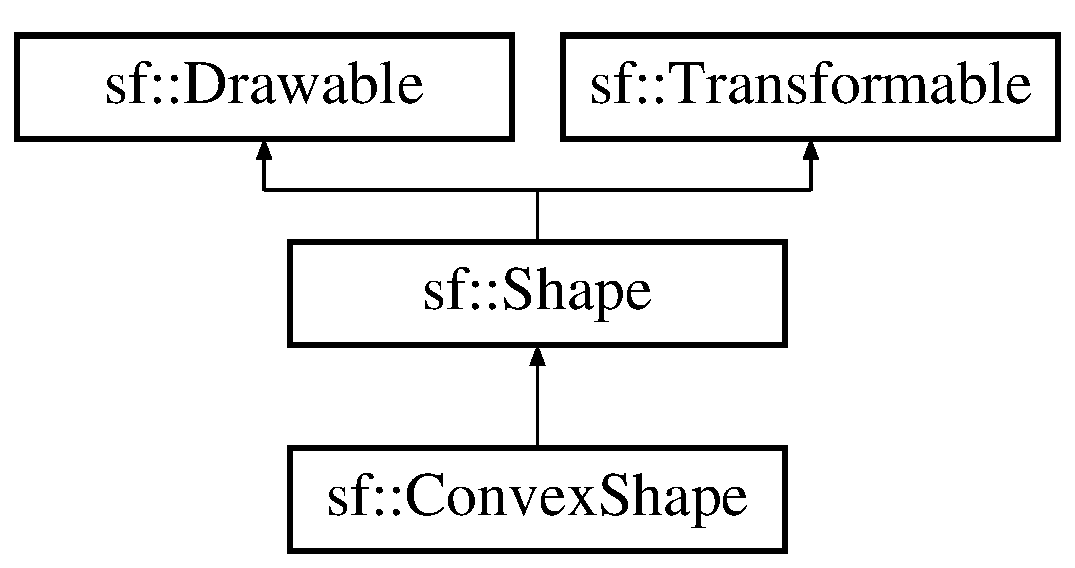
\includegraphics[height=3.000000cm]{classsf_1_1ConvexShape}
\end{center}
\end{figure}
\subsection*{Public Member Functions}
\begin{DoxyCompactItemize}
\item 
\hyperlink{classsf_1_1ConvexShape_a4f4686f57622bfbbe419ac1420b1432a}{Convex\-Shape} (unsigned int point\-Count=0)
\begin{DoxyCompactList}\small\item\em Default constructor. \end{DoxyCompactList}\item 
void \hyperlink{classsf_1_1ConvexShape_aea7c3f0f08f5cd457fe128a75b7c1e70}{set\-Point\-Count} (unsigned int count)
\begin{DoxyCompactList}\small\item\em Set the number of points of the polygon. \end{DoxyCompactList}\item 
virtual unsigned int \hyperlink{classsf_1_1ConvexShape_af81b86134fe54f2d50d9fab0db065ef1}{get\-Point\-Count} () const 
\begin{DoxyCompactList}\small\item\em Get the number of points of the polygon. \end{DoxyCompactList}\item 
void \hyperlink{classsf_1_1ConvexShape_ae5c7f87d0e776952e2ec6f0aa12ded31}{set\-Point} (unsigned int index, const \hyperlink{classsf_1_1Vector2}{Vector2f} \&point)
\begin{DoxyCompactList}\small\item\em Set the position of a point. \end{DoxyCompactList}\item 
virtual \hyperlink{classsf_1_1Vector2}{Vector2f} \hyperlink{classsf_1_1ConvexShape_ae2a18b837cd4454e340599a220c09a34}{get\-Point} (unsigned int index) const 
\begin{DoxyCompactList}\small\item\em Get the position of a point. \end{DoxyCompactList}\end{DoxyCompactItemize}
\subsection*{Additional Inherited Members}


\subsection{Detailed Description}
Specialized shape representing a convex polygon. 

This class inherits all the functions of \hyperlink{classsf_1_1Transformable}{sf\-::\-Transformable} (position, rotation, scale, bounds, ...) as well as the functions of \hyperlink{classsf_1_1Shape}{sf\-::\-Shape} (outline, color, texture, ...).

It is important to keep in mind that a convex shape must always be... convex, otherwise it may not be drawn correctly. Moreover, the points must be defined in order; using a random order would result in an incorrect shape.

Usage example\-: 
\begin{DoxyCode}
\hyperlink{classsf_1_1ConvexShape}{sf::ConvexShape} polygon;
polygon.\hyperlink{classsf_1_1ConvexShape_aea7c3f0f08f5cd457fe128a75b7c1e70}{setPointCount}(3);
polygon.\hyperlink{classsf_1_1ConvexShape_ae5c7f87d0e776952e2ec6f0aa12ded31}{setPoint}(0, \hyperlink{classsf_1_1Vector2}{sf::Vector2f}(0, 0));
polygon.\hyperlink{classsf_1_1ConvexShape_ae5c7f87d0e776952e2ec6f0aa12ded31}{setPoint}(1, \hyperlink{classsf_1_1Vector2}{sf::Vector2f}(0, 10));
polygon.\hyperlink{classsf_1_1ConvexShape_ae5c7f87d0e776952e2ec6f0aa12ded31}{setPoint}(2, \hyperlink{classsf_1_1Vector2}{sf::Vector2f}(25, 5));
polygon.\hyperlink{classsf_1_1Shape_a5978f41ee349ac3c52942996dcb184f7}{setOutlineColor}(\hyperlink{classsf_1_1Color_a127dbf55db9c07d0fa8f4bfcbb97594a}{sf::Color::Red});
polygon.\hyperlink{classsf_1_1Shape_a5ad336ad74fc1f567fce3b7e44cf87dc}{setOutlineThickness}(5);
polygon.\hyperlink{classsf_1_1Transformable_a4dbfb1a7c80688b0b4c477d706550208}{setPosition}(10, 20);
...
window.draw(polygon);
\end{DoxyCode}


\begin{DoxySeeAlso}{See Also}
\hyperlink{classsf_1_1Shape}{sf\-::\-Shape}, \hyperlink{classsf_1_1RectangleShape}{sf\-::\-Rectangle\-Shape}, \hyperlink{classsf_1_1CircleShape}{sf\-::\-Circle\-Shape} 
\end{DoxySeeAlso}


Definition at line 42 of file Convex\-Shape.\-hpp.



\subsection{Constructor \& Destructor Documentation}
\hypertarget{classsf_1_1ConvexShape_a4f4686f57622bfbbe419ac1420b1432a}{\index{sf\-::\-Convex\-Shape@{sf\-::\-Convex\-Shape}!Convex\-Shape@{Convex\-Shape}}
\index{Convex\-Shape@{Convex\-Shape}!sf::ConvexShape@{sf\-::\-Convex\-Shape}}
\subsubsection[{Convex\-Shape}]{\setlength{\rightskip}{0pt plus 5cm}sf\-::\-Convex\-Shape\-::\-Convex\-Shape (
\begin{DoxyParamCaption}
\item[{unsigned int}]{point\-Count = {\ttfamily 0}}
\end{DoxyParamCaption}
)\hspace{0.3cm}{\ttfamily [explicit]}}}\label{classsf_1_1ConvexShape_a4f4686f57622bfbbe419ac1420b1432a}


Default constructor. 


\begin{DoxyParams}{Parameters}
{\em point\-Count} & Number of points of the polygon \\
\hline
\end{DoxyParams}


\subsection{Member Function Documentation}
\hypertarget{classsf_1_1ConvexShape_ae2a18b837cd4454e340599a220c09a34}{\index{sf\-::\-Convex\-Shape@{sf\-::\-Convex\-Shape}!get\-Point@{get\-Point}}
\index{get\-Point@{get\-Point}!sf::ConvexShape@{sf\-::\-Convex\-Shape}}
\subsubsection[{get\-Point}]{\setlength{\rightskip}{0pt plus 5cm}virtual {\bf Vector2f} sf\-::\-Convex\-Shape\-::get\-Point (
\begin{DoxyParamCaption}
\item[{unsigned int}]{index}
\end{DoxyParamCaption}
) const\hspace{0.3cm}{\ttfamily [virtual]}}}\label{classsf_1_1ConvexShape_ae2a18b837cd4454e340599a220c09a34}


Get the position of a point. 

The result is undefined if {\itshape index} is out of the valid range.


\begin{DoxyParams}{Parameters}
{\em index} & Index of the point to get, in range \mbox{[}0 .. \hyperlink{classsf_1_1ConvexShape_af81b86134fe54f2d50d9fab0db065ef1}{get\-Point\-Count()} -\/ 1\mbox{]}\\
\hline
\end{DoxyParams}
\begin{DoxyReturn}{Returns}
Position of the index-\/th point of the polygon
\end{DoxyReturn}
\begin{DoxySeeAlso}{See Also}
\hyperlink{classsf_1_1ConvexShape_ae5c7f87d0e776952e2ec6f0aa12ded31}{set\-Point} 
\end{DoxySeeAlso}


Implements \hyperlink{classsf_1_1Shape_a397f3b4cdb7ad98cdc6c034816c652d2}{sf\-::\-Shape}.

\hypertarget{classsf_1_1ConvexShape_af81b86134fe54f2d50d9fab0db065ef1}{\index{sf\-::\-Convex\-Shape@{sf\-::\-Convex\-Shape}!get\-Point\-Count@{get\-Point\-Count}}
\index{get\-Point\-Count@{get\-Point\-Count}!sf::ConvexShape@{sf\-::\-Convex\-Shape}}
\subsubsection[{get\-Point\-Count}]{\setlength{\rightskip}{0pt plus 5cm}virtual unsigned int sf\-::\-Convex\-Shape\-::get\-Point\-Count (
\begin{DoxyParamCaption}
{}
\end{DoxyParamCaption}
) const\hspace{0.3cm}{\ttfamily [virtual]}}}\label{classsf_1_1ConvexShape_af81b86134fe54f2d50d9fab0db065ef1}


Get the number of points of the polygon. 

\begin{DoxyReturn}{Returns}
Number of points of the polygon
\end{DoxyReturn}
\begin{DoxySeeAlso}{See Also}
\hyperlink{classsf_1_1ConvexShape_aea7c3f0f08f5cd457fe128a75b7c1e70}{set\-Point\-Count} 
\end{DoxySeeAlso}


Implements \hyperlink{classsf_1_1Shape_ad84e1b675ecd270ad8151aea4e271a78}{sf\-::\-Shape}.

\hypertarget{classsf_1_1ConvexShape_ae5c7f87d0e776952e2ec6f0aa12ded31}{\index{sf\-::\-Convex\-Shape@{sf\-::\-Convex\-Shape}!set\-Point@{set\-Point}}
\index{set\-Point@{set\-Point}!sf::ConvexShape@{sf\-::\-Convex\-Shape}}
\subsubsection[{set\-Point}]{\setlength{\rightskip}{0pt plus 5cm}void sf\-::\-Convex\-Shape\-::set\-Point (
\begin{DoxyParamCaption}
\item[{unsigned int}]{index, }
\item[{const {\bf Vector2f} \&}]{point}
\end{DoxyParamCaption}
)}}\label{classsf_1_1ConvexShape_ae5c7f87d0e776952e2ec6f0aa12ded31}


Set the position of a point. 

Don't forget that the polygon must remain convex, and the points need to stay ordered! set\-Point\-Count must be called first in order to set the total number of points. The result is undefined if {\itshape index} is out of the valid range.


\begin{DoxyParams}{Parameters}
{\em index} & Index of the point to change, in range \mbox{[}0 .. \hyperlink{classsf_1_1ConvexShape_af81b86134fe54f2d50d9fab0db065ef1}{get\-Point\-Count()} -\/ 1\mbox{]} \\
\hline
{\em point} & New position of the point\\
\hline
\end{DoxyParams}
\begin{DoxySeeAlso}{See Also}
\hyperlink{classsf_1_1ConvexShape_ae2a18b837cd4454e340599a220c09a34}{get\-Point} 
\end{DoxySeeAlso}
\hypertarget{classsf_1_1ConvexShape_aea7c3f0f08f5cd457fe128a75b7c1e70}{\index{sf\-::\-Convex\-Shape@{sf\-::\-Convex\-Shape}!set\-Point\-Count@{set\-Point\-Count}}
\index{set\-Point\-Count@{set\-Point\-Count}!sf::ConvexShape@{sf\-::\-Convex\-Shape}}
\subsubsection[{set\-Point\-Count}]{\setlength{\rightskip}{0pt plus 5cm}void sf\-::\-Convex\-Shape\-::set\-Point\-Count (
\begin{DoxyParamCaption}
\item[{unsigned int}]{count}
\end{DoxyParamCaption}
)}}\label{classsf_1_1ConvexShape_aea7c3f0f08f5cd457fe128a75b7c1e70}


Set the number of points of the polygon. 

{\itshape count} must be greater than 2 to define a valid shape.


\begin{DoxyParams}{Parameters}
{\em count} & New number of points of the polygon\\
\hline
\end{DoxyParams}
\begin{DoxySeeAlso}{See Also}
\hyperlink{classsf_1_1ConvexShape_af81b86134fe54f2d50d9fab0db065ef1}{get\-Point\-Count} 
\end{DoxySeeAlso}


The documentation for this class was generated from the following file\-:\begin{DoxyCompactItemize}
\item 
/home/z\-Zelman/\-Dropbox/\-Placeholder-\/\-R\-T\-S/\-S\-F\-M\-L-\/2.\-1/include/\-S\-F\-M\-L/\-Graphics/Convex\-Shape.\-hpp\end{DoxyCompactItemize}

\hypertarget{classCPhysicsEngine}{\section{C\-Physics\-Engine Class Reference}
\label{classCPhysicsEngine}\index{C\-Physics\-Engine@{C\-Physics\-Engine}}
}
Inheritance diagram for C\-Physics\-Engine\-:\begin{figure}[H]
\begin{center}
\leavevmode
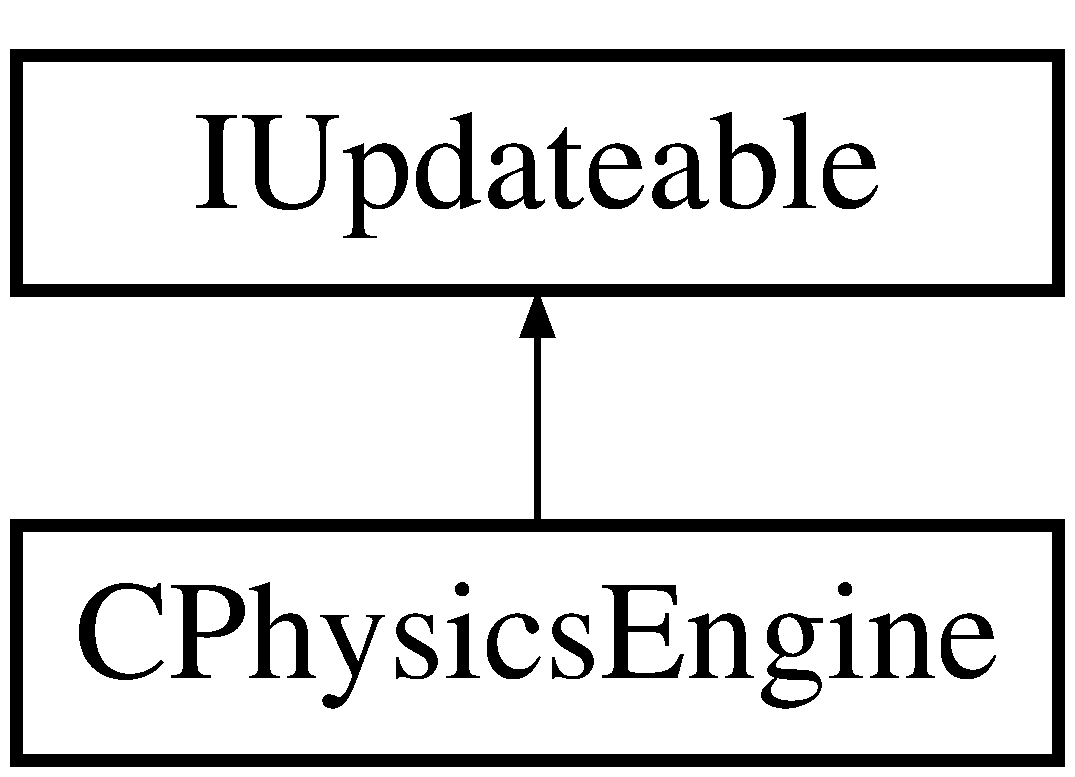
\includegraphics[height=2.000000cm]{classCPhysicsEngine}
\end{center}
\end{figure}
\subsection*{Public Member Functions}
\begin{DoxyCompactItemize}
\item 
\hypertarget{classCPhysicsEngine_a33fb6680b9f22590802f613f1c707abd}{{\bfseries C\-Physics\-Engine} (\hyperlink{classCTile__Container}{C\-Tile\-\_\-\-Container} $\ast$p\-Tile\-\_\-\-Container, \hyperlink{classCRoom__Container}{C\-Room\-\_\-\-Container} $\ast$p\-Room\-\_\-\-Container, \hyperlink{classCUnit__Container}{C\-Unit\-\_\-\-Container} $\ast$p\-Unit\-\_\-\-Container)}\label{classCPhysicsEngine_a33fb6680b9f22590802f613f1c707abd}

\item 
\hypertarget{classCPhysicsEngine_abc493897bbdb15e6787a25478730f1f5}{void {\bfseries update} ()}\label{classCPhysicsEngine_abc493897bbdb15e6787a25478730f1f5}

\end{DoxyCompactItemize}


\subsection{Detailed Description}


Definition at line 19 of file C\-Physics\-Engine.\-h.



The documentation for this class was generated from the following files\-:\begin{DoxyCompactItemize}
\item 
/home/z\-Zelman/\-Dropbox/\-Placeholder-\/\-R\-T\-S/src/\-Physics/C\-Physics\-Engine.\-h\item 
/home/z\-Zelman/\-Dropbox/\-Placeholder-\/\-R\-T\-S/src/\-Physics/C\-Physics\-Engine.\-cpp\end{DoxyCompactItemize}

\hypertarget{classCQuadTree}{\section{C\-Quad\-Tree Class Reference}
\label{classCQuadTree}\index{C\-Quad\-Tree@{C\-Quad\-Tree}}
}
\subsection*{Public Member Functions}
\begin{DoxyCompactItemize}
\item 
\hypertarget{classCQuadTree_a508176d23f4bcb255ca06bf70edce638}{{\bfseries C\-Quad\-Tree} (int level, \hyperlink{classsf_1_1Rect}{sf\-::\-Int\-Rect} $\ast$bounds)}\label{classCQuadTree_a508176d23f4bcb255ca06bf70edce638}

\item 
\hypertarget{classCQuadTree_ab4cf0e58d782f7674eae21a1e56fa6d2}{void {\bfseries clear} ()}\label{classCQuadTree_ab4cf0e58d782f7674eae21a1e56fa6d2}

\item 
\hypertarget{classCQuadTree_ac0ded7f002956e96269743dde8833cab}{void {\bfseries insert} (\hyperlink{classARenderable}{A\-Renderable} $\ast$p\-Object)}\label{classCQuadTree_ac0ded7f002956e96269743dde8833cab}

\item 
\hypertarget{classCQuadTree_a5bd034b9f4860bcaa4fdfc65391251eb}{void {\bfseries retrieve} (std\-::list$<$ \hyperlink{classARenderable}{A\-Renderable} $\ast$ $>$ $\ast$returned\-Objects, \hyperlink{classARenderable}{A\-Renderable} $\ast$p\-Object)}\label{classCQuadTree_a5bd034b9f4860bcaa4fdfc65391251eb}

\end{DoxyCompactItemize}


\subsection{Detailed Description}


Definition at line 34 of file C\-Quad\-Tree.\-h.



The documentation for this class was generated from the following files\-:\begin{DoxyCompactItemize}
\item 
/home/z\-Zelman/\-Dropbox/\-Placeholder-\/\-R\-T\-S/src/\-Physics/C\-Quad\-Tree.\-h\item 
/home/z\-Zelman/\-Dropbox/\-Placeholder-\/\-R\-T\-S/src/\-Physics/C\-Quad\-Tree.\-cpp\end{DoxyCompactItemize}

\hypertarget{classCRenderEngine}{\section{C\-Render\-Engine Class Reference}
\label{classCRenderEngine}\index{C\-Render\-Engine@{C\-Render\-Engine}}
}
\subsection*{Public Member Functions}
\begin{DoxyCompactItemize}
\item 
\hypertarget{classCRenderEngine_af6f482173b9ee00d217d15866dc6376b}{{\bfseries C\-Render\-Engine} (\hyperlink{classsf_1_1RenderWindow}{sf\-::\-Render\-Window} $\ast$p\-Window, \hyperlink{classCRoom__Container}{C\-Room\-\_\-\-Container} $\ast$p\-Room\-\_\-\-Container, \hyperlink{classCUnit__Container}{C\-Unit\-\_\-\-Container} $\ast$p\-Unit\-\_\-\-Container, \hyperlink{classCTile__Container}{C\-Tile\-\_\-\-Container} $\ast$p\-Tile\-\_\-\-Container, \hyperlink{classCHUD}{C\-H\-U\-D} $\ast$p\-H\-U\-D)}\label{classCRenderEngine_af6f482173b9ee00d217d15866dc6376b}

\item 
\hypertarget{classCRenderEngine_a38c058de2a8b54f208decdaa7b799ada}{void {\bfseries render} ()}\label{classCRenderEngine_a38c058de2a8b54f208decdaa7b799ada}

\end{DoxyCompactItemize}


\subsection{Detailed Description}


Definition at line 19 of file C\-Render\-Engine.\-h.



The documentation for this class was generated from the following files\-:\begin{DoxyCompactItemize}
\item 
/home/z\-Zelman/\-Dropbox/\-Placeholder-\/\-R\-T\-S/src/\-Graphics/C\-Render\-Engine.\-h\item 
/home/z\-Zelman/\-Dropbox/\-Placeholder-\/\-R\-T\-S/src/\-Graphics/C\-Render\-Engine.\-cpp\end{DoxyCompactItemize}

\hypertarget{classCRoom}{\section{C\-Room Class Reference}
\label{classCRoom}\index{C\-Room@{C\-Room}}
}
Inheritance diagram for C\-Room\-:\begin{figure}[H]
\begin{center}
\leavevmode
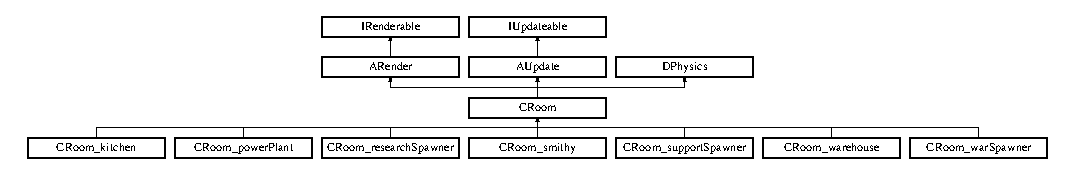
\includegraphics[height=1.904762cm]{classCRoom}
\end{center}
\end{figure}
\subsection*{Public Member Functions}
\begin{DoxyCompactItemize}
\item 
\hypertarget{classCRoom_a238c3071e90bfb973b8b6f8eb9dc44c9}{{\bfseries C\-Room} (\hyperlink{classCTexture}{C\-Texture} $\ast$p\-Texture, const \hyperlink{classsf_1_1Vector2}{sf\-::\-Vector2}$<$ int $>$ \&curr\-Sub)}\label{classCRoom_a238c3071e90bfb973b8b6f8eb9dc44c9}

\item 
\hypertarget{classCRoom_a554288f277403d72aa6eae4139096996}{virtual void {\bfseries update} ()}\label{classCRoom_a554288f277403d72aa6eae4139096996}

\item 
\hypertarget{classCRoom_ada8b3e3ffc799354d377df71e5ee6b7d}{void {\bfseries step\-Normally} ()}\label{classCRoom_ada8b3e3ffc799354d377df71e5ee6b7d}

\end{DoxyCompactItemize}
\subsection*{Additional Inherited Members}


\subsection{Detailed Description}


Definition at line 21 of file C\-Room.\-h.



The documentation for this class was generated from the following files\-:\begin{DoxyCompactItemize}
\item 
/home/z\-Zelman/\-Dropbox/\-Placeholder-\/\-R\-T\-S/src/\-Rooms/C\-Room.\-h\item 
/home/z\-Zelman/\-Dropbox/\-Placeholder-\/\-R\-T\-S/src/\-Rooms/C\-Room.\-cpp\end{DoxyCompactItemize}

\hypertarget{classCRoom__Container}{\section{C\-Room\-\_\-\-Container Class Reference}
\label{classCRoom__Container}\index{C\-Room\-\_\-\-Container@{C\-Room\-\_\-\-Container}}
}
Inheritance diagram for C\-Room\-\_\-\-Container\-:\begin{figure}[H]
\begin{center}
\leavevmode
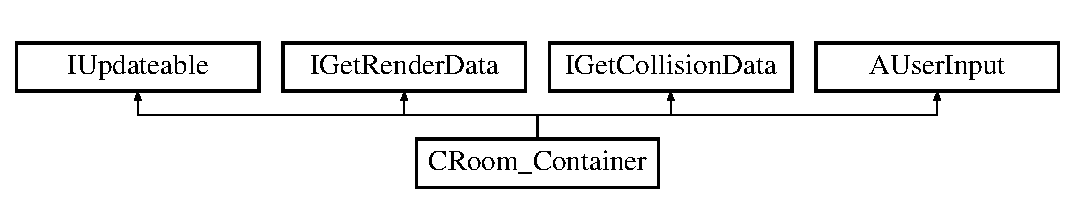
\includegraphics[height=1.836066cm]{classCRoom__Container}
\end{center}
\end{figure}
\subsection*{Public Member Functions}
\begin{DoxyCompactItemize}
\item 
\hypertarget{classCRoom__Container_a3a1f638e223c661251d679d119a8a0c5}{{\bfseries C\-Room\-\_\-\-Container} (\hyperlink{classsf_1_1RenderWindow}{sf\-::\-Render\-Window} $\ast$p\-Window, \hyperlink{classCTile__Container}{C\-Tile\-\_\-\-Container} $\ast$p\-Grid)}\label{classCRoom__Container_a3a1f638e223c661251d679d119a8a0c5}

\item 
\hypertarget{classCRoom__Container_a4487394b5b73570abf3731200129e507}{const \hyperlink{structSNumRooms}{S\-Num\-Rooms} $\ast$ {\bfseries get\-Num\-Rooms} () const }\label{classCRoom__Container_a4487394b5b73570abf3731200129e507}

\item 
\hypertarget{classCRoom__Container_a976c43bd83d5416c3f3d286d09ebf89d}{void {\bfseries update} ()}\label{classCRoom__Container_a976c43bd83d5416c3f3d286d09ebf89d}

\item 
\hypertarget{classCRoom__Container_a170af863c917d336c1497fd031d79c6f}{void {\bfseries render} ()}\label{classCRoom__Container_a170af863c917d336c1497fd031d79c6f}

\item 
\hypertarget{classCRoom__Container_a8119bbe9405d6f151e8fd06e441e7eb5}{void {\bfseries get\-Collisiondata} (std\-::list$<$ \hyperlink{classARender}{A\-Render} $\ast$ $>$ $\ast$p\-List)}\label{classCRoom__Container_a8119bbe9405d6f151e8fd06e441e7eb5}

\item 
\hypertarget{classCRoom__Container_a96edd6800ff447f90fec9ae116eda34e}{void {\bfseries get\-Render\-Data} (std\-::list$<$ \hyperlink{classARender}{A\-Render} $\ast$ $>$ $\ast$p\-List)}\label{classCRoom__Container_a96edd6800ff447f90fec9ae116eda34e}

\item 
\hypertarget{classCRoom__Container_aa220dc3fd30384ef9d3b13b0f7c0a417}{bool {\bfseries user\-Input\-\_\-key\-Press} (\hyperlink{classsf_1_1Event}{sf\-::\-Event} $\ast$p\-Event)}\label{classCRoom__Container_aa220dc3fd30384ef9d3b13b0f7c0a417}

\item 
\hypertarget{classCRoom__Container_a85bb9fcebc84e71bb90fb5c7d7c201a6}{bool {\bfseries user\-Input\-\_\-key\-Release} (\hyperlink{classsf_1_1Event}{sf\-::\-Event} $\ast$p\-Event)}\label{classCRoom__Container_a85bb9fcebc84e71bb90fb5c7d7c201a6}

\item 
\hypertarget{classCRoom__Container_a84080540b5cb7a400662aba47fee60fc}{bool {\bfseries user\-Input\-\_\-mouse\-Press} (\hyperlink{classsf_1_1Event}{sf\-::\-Event} $\ast$p\-Event)}\label{classCRoom__Container_a84080540b5cb7a400662aba47fee60fc}

\item 
\hypertarget{classCRoom__Container_adb9e0db332c48e7baabf55d7e14ac512}{bool {\bfseries user\-Input\-\_\-mouse\-Release} (\hyperlink{classsf_1_1Event}{sf\-::\-Event} $\ast$p\-Event)}\label{classCRoom__Container_adb9e0db332c48e7baabf55d7e14ac512}

\item 
\hypertarget{classCRoom__Container_a2eb1c5bc2aef2804cb15cbedd5fc649a}{bool {\bfseries is\-Collision} (const \hyperlink{classsf_1_1Rect}{sf\-::\-Rect}$<$ float $>$ \&rect, \hyperlink{classCRoom}{C\-Room} $\ast$\&p\-Room)}\label{classCRoom__Container_a2eb1c5bc2aef2804cb15cbedd5fc649a}

\end{DoxyCompactItemize}
\subsection*{Additional Inherited Members}


\subsection{Detailed Description}


Definition at line 41 of file C\-Room\-\_\-\-Container.\-h.



The documentation for this class was generated from the following files\-:\begin{DoxyCompactItemize}
\item 
/home/z\-Zelman/\-Dropbox/\-Placeholder-\/\-R\-T\-S/src/\-Rooms/C\-Room\-\_\-\-Container.\-h\item 
/home/z\-Zelman/\-Dropbox/\-Placeholder-\/\-R\-T\-S/src/\-Rooms/C\-Room\-\_\-\-Container.\-cpp\end{DoxyCompactItemize}

\hypertarget{classCRoom__kitchen}{\section{C\-Room\-\_\-kitchen Class Reference}
\label{classCRoom__kitchen}\index{C\-Room\-\_\-kitchen@{C\-Room\-\_\-kitchen}}
}
Inheritance diagram for C\-Room\-\_\-kitchen\-:\begin{figure}[H]
\begin{center}
\leavevmode
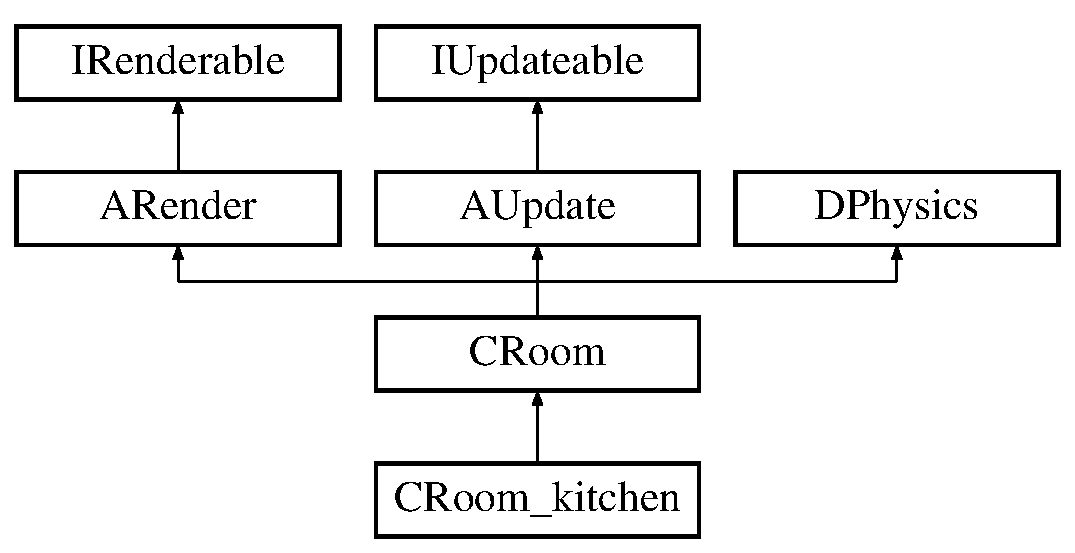
\includegraphics[height=4.000000cm]{classCRoom__kitchen}
\end{center}
\end{figure}
\subsection*{Public Member Functions}
\begin{DoxyCompactItemize}
\item 
\hypertarget{classCRoom__kitchen_a5bb2e465e287208513ecc4e30caf1977}{{\bfseries C\-Room\-\_\-kitchen} (\hyperlink{classsf_1_1RenderWindow}{sf\-::\-Render\-Window} $\ast$p\-Window, \hyperlink{classCTexture}{C\-Texture} $\ast$p\-Texture, const \hyperlink{classsf_1_1Vector2}{sf\-::\-Vector2}$<$ int $>$ \&curr\-Sub)}\label{classCRoom__kitchen_a5bb2e465e287208513ecc4e30caf1977}

\item 
\hypertarget{classCRoom__kitchen_a6c3ad2d5a04a0b1ed566e6d1108a923c}{void {\bfseries update} ()}\label{classCRoom__kitchen_a6c3ad2d5a04a0b1ed566e6d1108a923c}

\end{DoxyCompactItemize}
\subsection*{Additional Inherited Members}


\subsection{Detailed Description}


Definition at line 13 of file C\-Room\-\_\-kitchen.\-h.



The documentation for this class was generated from the following files\-:\begin{DoxyCompactItemize}
\item 
/home/z\-Zelman/\-Dropbox/\-Placeholder-\/\-R\-T\-S/src/\-Rooms/C\-Room\-\_\-kitchen.\-h\item 
/home/z\-Zelman/\-Dropbox/\-Placeholder-\/\-R\-T\-S/src/\-Rooms/C\-Room\-\_\-kitchen.\-cpp\end{DoxyCompactItemize}

\hypertarget{classCRoom__powerPlant}{\section{C\-Room\-\_\-power\-Plant Class Reference}
\label{classCRoom__powerPlant}\index{C\-Room\-\_\-power\-Plant@{C\-Room\-\_\-power\-Plant}}
}
Inheritance diagram for C\-Room\-\_\-power\-Plant\-:\begin{figure}[H]
\begin{center}
\leavevmode
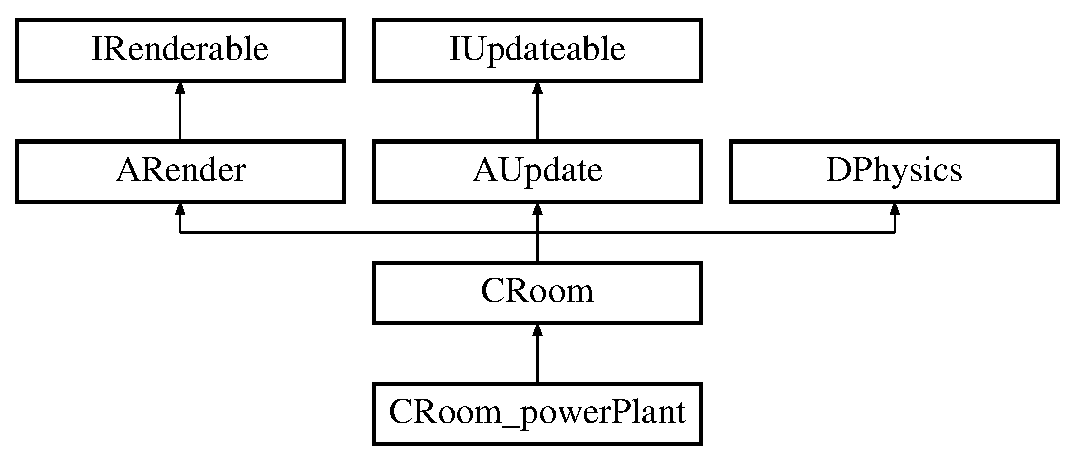
\includegraphics[height=4.000000cm]{classCRoom__powerPlant}
\end{center}
\end{figure}
\subsection*{Public Member Functions}
\begin{DoxyCompactItemize}
\item 
\hypertarget{classCRoom__powerPlant_af7d6452c5f0b7bc4b0050ea7765bc223}{{\bfseries C\-Room\-\_\-power\-Plant} (\hyperlink{classCTexture}{C\-Texture} $\ast$p\-Texture, const \hyperlink{classsf_1_1Vector2}{sf\-::\-Vector2}$<$ int $>$ \&curr\-Sub)}\label{classCRoom__powerPlant_af7d6452c5f0b7bc4b0050ea7765bc223}

\item 
\hypertarget{classCRoom__powerPlant_a8861ab0e2382e25b0130b29326717121}{void {\bfseries update} ()}\label{classCRoom__powerPlant_a8861ab0e2382e25b0130b29326717121}

\end{DoxyCompactItemize}
\subsection*{Additional Inherited Members}


\subsection{Detailed Description}


Definition at line 13 of file C\-Room\-\_\-power\-Plant.\-h.



The documentation for this class was generated from the following files\-:\begin{DoxyCompactItemize}
\item 
/home/z\-Zelman/\-Dropbox/\-Placeholder-\/\-R\-T\-S/src/\-Rooms/C\-Room\-\_\-power\-Plant.\-h\item 
/home/z\-Zelman/\-Dropbox/\-Placeholder-\/\-R\-T\-S/src/\-Rooms/C\-Room\-\_\-power\-Plant.\-cpp\end{DoxyCompactItemize}

\hypertarget{classCRoom__researchSpawner}{\section{C\-Room\-\_\-research\-Spawner Class Reference}
\label{classCRoom__researchSpawner}\index{C\-Room\-\_\-research\-Spawner@{C\-Room\-\_\-research\-Spawner}}
}
Inheritance diagram for C\-Room\-\_\-research\-Spawner\-:\begin{figure}[H]
\begin{center}
\leavevmode
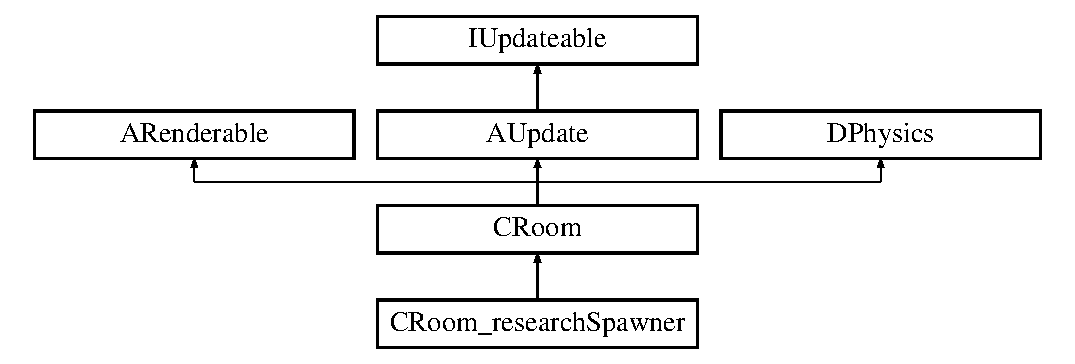
\includegraphics[height=4.000000cm]{classCRoom__researchSpawner}
\end{center}
\end{figure}
\subsection*{Public Member Functions}
\begin{DoxyCompactItemize}
\item 
\hypertarget{classCRoom__researchSpawner_a4ee41a903b9bdd6c7a559bf72d78b135}{{\bfseries C\-Room\-\_\-research\-Spawner} (\hyperlink{classCTexture}{C\-Texture} $\ast$p\-Texture, const \hyperlink{classsf_1_1Vector2}{sf\-::\-Vector2}$<$ int $>$ \&curr\-Sub)}\label{classCRoom__researchSpawner_a4ee41a903b9bdd6c7a559bf72d78b135}

\item 
\hypertarget{classCRoom__researchSpawner_ab565078eeec1d2dded6f19a91e322665}{void {\bfseries update} ()}\label{classCRoom__researchSpawner_ab565078eeec1d2dded6f19a91e322665}

\end{DoxyCompactItemize}
\subsection*{Additional Inherited Members}


\subsection{Detailed Description}


Definition at line 13 of file C\-Room\-\_\-research\-Spawner.\-h.



The documentation for this class was generated from the following files\-:\begin{DoxyCompactItemize}
\item 
/home/z\-Zelman/\-Dropbox/\-Placeholder-\/\-R\-T\-S/src/\-Rooms/C\-Room\-\_\-research\-Spawner.\-h\item 
/home/z\-Zelman/\-Dropbox/\-Placeholder-\/\-R\-T\-S/src/\-Rooms/C\-Room\-\_\-research\-Spawner.\-cpp\end{DoxyCompactItemize}

\hypertarget{classCRoom__smithy}{\section{C\-Room\-\_\-smithy Class Reference}
\label{classCRoom__smithy}\index{C\-Room\-\_\-smithy@{C\-Room\-\_\-smithy}}
}
Inheritance diagram for C\-Room\-\_\-smithy\-:\begin{figure}[H]
\begin{center}
\leavevmode
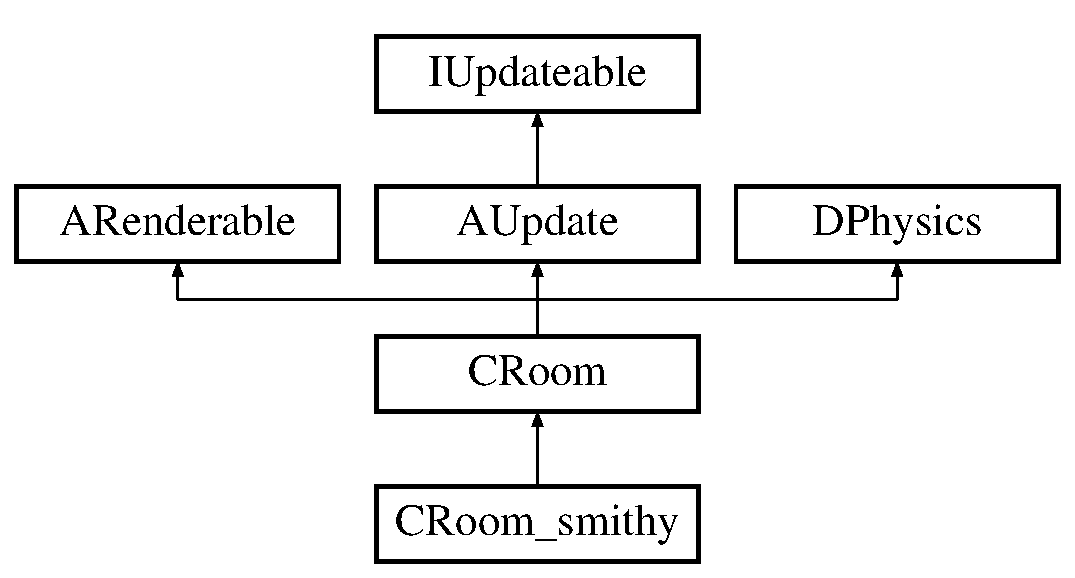
\includegraphics[height=4.000000cm]{classCRoom__smithy}
\end{center}
\end{figure}
\subsection*{Public Member Functions}
\begin{DoxyCompactItemize}
\item 
\hypertarget{classCRoom__smithy_abb70a37327425c0b7f83f3e7c8ef5a9b}{{\bfseries C\-Room\-\_\-smithy} (\hyperlink{classCTexture}{C\-Texture} $\ast$p\-Texture, const \hyperlink{classsf_1_1Vector2}{sf\-::\-Vector2}$<$ int $>$ \&curr\-Sub)}\label{classCRoom__smithy_abb70a37327425c0b7f83f3e7c8ef5a9b}

\item 
\hypertarget{classCRoom__smithy_a5e7be1eed9a469748fcd6ed7ecd3c772}{void {\bfseries update} ()}\label{classCRoom__smithy_a5e7be1eed9a469748fcd6ed7ecd3c772}

\end{DoxyCompactItemize}
\subsection*{Additional Inherited Members}


\subsection{Detailed Description}


Definition at line 13 of file C\-Room\-\_\-smithy.\-h.



The documentation for this class was generated from the following files\-:\begin{DoxyCompactItemize}
\item 
/home/z\-Zelman/\-Dropbox/\-Placeholder-\/\-R\-T\-S/src/\-Rooms/C\-Room\-\_\-smithy.\-h\item 
/home/z\-Zelman/\-Dropbox/\-Placeholder-\/\-R\-T\-S/src/\-Rooms/C\-Room\-\_\-smithy.\-cpp\end{DoxyCompactItemize}

\hypertarget{classCRoom__supportSpawner}{\section{C\-Room\-\_\-support\-Spawner Class Reference}
\label{classCRoom__supportSpawner}\index{C\-Room\-\_\-support\-Spawner@{C\-Room\-\_\-support\-Spawner}}
}
Inheritance diagram for C\-Room\-\_\-support\-Spawner\-:\begin{figure}[H]
\begin{center}
\leavevmode
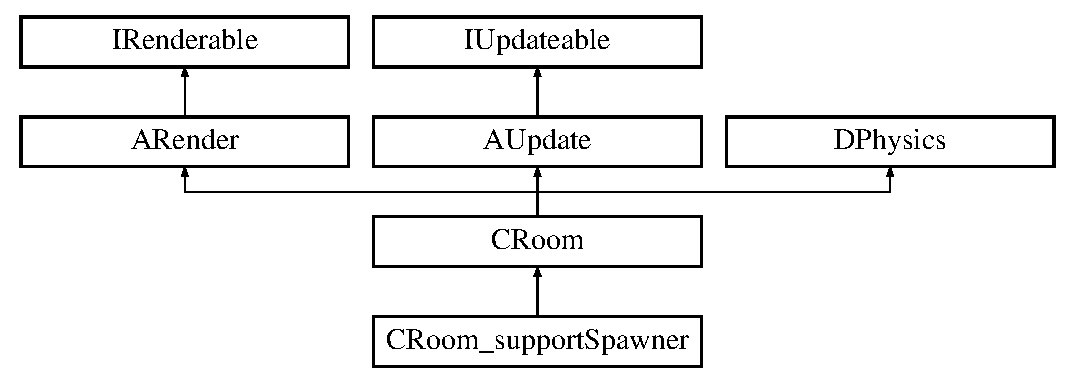
\includegraphics[height=4.000000cm]{classCRoom__supportSpawner}
\end{center}
\end{figure}
\subsection*{Public Member Functions}
\begin{DoxyCompactItemize}
\item 
\hypertarget{classCRoom__supportSpawner_a9cc8c824228709db6db90b8dd75988cf}{{\bfseries C\-Room\-\_\-support\-Spawner} (\hyperlink{classCTexture}{C\-Texture} $\ast$p\-Texture, const \hyperlink{classsf_1_1Vector2}{sf\-::\-Vector2}$<$ int $>$ \&curr\-Sub)}\label{classCRoom__supportSpawner_a9cc8c824228709db6db90b8dd75988cf}

\item 
\hypertarget{classCRoom__supportSpawner_a509e95652394c868388b79b2e98d67f0}{void {\bfseries update} ()}\label{classCRoom__supportSpawner_a509e95652394c868388b79b2e98d67f0}

\end{DoxyCompactItemize}
\subsection*{Additional Inherited Members}


\subsection{Detailed Description}


Definition at line 13 of file C\-Room\-\_\-support\-Spawner.\-h.



The documentation for this class was generated from the following files\-:\begin{DoxyCompactItemize}
\item 
/home/z\-Zelman/\-Dropbox/\-Placeholder-\/\-R\-T\-S/src/\-Rooms/C\-Room\-\_\-support\-Spawner.\-h\item 
/home/z\-Zelman/\-Dropbox/\-Placeholder-\/\-R\-T\-S/src/\-Rooms/C\-Room\-\_\-support\-Spawner.\-cpp\end{DoxyCompactItemize}

\hypertarget{classCRoom__warehouse}{\section{C\-Room\-\_\-warehouse Class Reference}
\label{classCRoom__warehouse}\index{C\-Room\-\_\-warehouse@{C\-Room\-\_\-warehouse}}
}
Inheritance diagram for C\-Room\-\_\-warehouse\-:\begin{figure}[H]
\begin{center}
\leavevmode
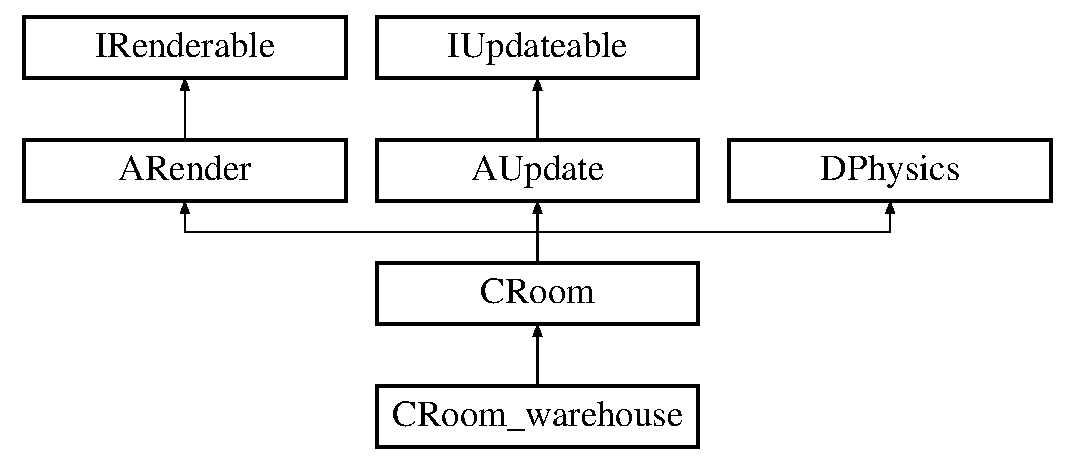
\includegraphics[height=4.000000cm]{classCRoom__warehouse}
\end{center}
\end{figure}
\subsection*{Public Member Functions}
\begin{DoxyCompactItemize}
\item 
\hypertarget{classCRoom__warehouse_a181b6becc788b6cec95e8f73116e7a30}{{\bfseries C\-Room\-\_\-warehouse} (\hyperlink{classCTexture}{C\-Texture} $\ast$p\-Texture, const \hyperlink{classsf_1_1Vector2}{sf\-::\-Vector2}$<$ int $>$ \&curr\-Sub)}\label{classCRoom__warehouse_a181b6becc788b6cec95e8f73116e7a30}

\item 
\hypertarget{classCRoom__warehouse_ab4f3d3a87421ef23febd6f259341d4cd}{void {\bfseries update} ()}\label{classCRoom__warehouse_ab4f3d3a87421ef23febd6f259341d4cd}

\end{DoxyCompactItemize}
\subsection*{Additional Inherited Members}


\subsection{Detailed Description}


Definition at line 15 of file C\-Room\-\_\-warehouse.\-h.



The documentation for this class was generated from the following files\-:\begin{DoxyCompactItemize}
\item 
/home/z\-Zelman/\-Dropbox/\-Placeholder-\/\-R\-T\-S/src/\-Rooms/C\-Room\-\_\-warehouse.\-h\item 
/home/z\-Zelman/\-Dropbox/\-Placeholder-\/\-R\-T\-S/src/\-Rooms/C\-Room\-\_\-warehouse.\-cpp\end{DoxyCompactItemize}

\hypertarget{classCRoom__warSpawner}{\section{C\-Room\-\_\-war\-Spawner Class Reference}
\label{classCRoom__warSpawner}\index{C\-Room\-\_\-war\-Spawner@{C\-Room\-\_\-war\-Spawner}}
}
Inheritance diagram for C\-Room\-\_\-war\-Spawner\-:\begin{figure}[H]
\begin{center}
\leavevmode
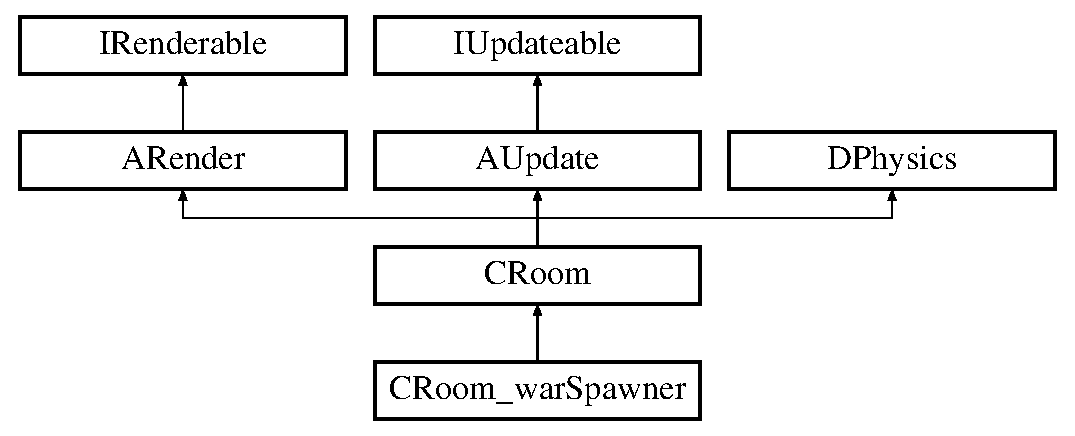
\includegraphics[height=4.000000cm]{classCRoom__warSpawner}
\end{center}
\end{figure}
\subsection*{Public Member Functions}
\begin{DoxyCompactItemize}
\item 
\hypertarget{classCRoom__warSpawner_ac5c593c176b3644c4e0240e31281e6c9}{{\bfseries C\-Room\-\_\-war\-Spawner} (\hyperlink{classCTexture}{C\-Texture} $\ast$p\-Texture, const \hyperlink{classsf_1_1Vector2}{sf\-::\-Vector2}$<$ int $>$ \&curr\-Sub)}\label{classCRoom__warSpawner_ac5c593c176b3644c4e0240e31281e6c9}

\item 
\hypertarget{classCRoom__warSpawner_a67388a7401fddf2655945364dc42f837}{void {\bfseries update} ()}\label{classCRoom__warSpawner_a67388a7401fddf2655945364dc42f837}

\end{DoxyCompactItemize}
\subsection*{Additional Inherited Members}


\subsection{Detailed Description}


Definition at line 13 of file C\-Room\-\_\-war\-Spawner.\-h.



The documentation for this class was generated from the following files\-:\begin{DoxyCompactItemize}
\item 
/home/z\-Zelman/\-Dropbox/\-Placeholder-\/\-R\-T\-S/src/\-Rooms/C\-Room\-\_\-war\-Spawner.\-h\item 
/home/z\-Zelman/\-Dropbox/\-Placeholder-\/\-R\-T\-S/src/\-Rooms/C\-Room\-\_\-war\-Spawner.\-cpp\end{DoxyCompactItemize}

\hypertarget{classCSpawner}{\section{C\-Spawner Class Reference}
\label{classCSpawner}\index{C\-Spawner@{C\-Spawner}}
}


{\ttfamily \#include $<$C\-Spawner.\-h$>$}

\subsection*{Public Member Functions}
\begin{DoxyCompactItemize}
\item 
\hypertarget{classCSpawner_a72b2b6ec16e6f78685c4412c821942ba}{{\bfseries C\-Spawner} (\hyperlink{classCRoom__Container}{C\-Room\-\_\-\-Container} $\ast$p\-Room\-\_\-\-Container)}\label{classCSpawner_a72b2b6ec16e6f78685c4412c821942ba}

\item 
\hypertarget{classCSpawner_a6af5e85072a0bad2defa58c810de4033}{void {\bfseries spawn\-Room\-\_\-warehouse} (int x, int y)}\label{classCSpawner_a6af5e85072a0bad2defa58c810de4033}

\item 
\hypertarget{classCSpawner_a9fc39b2d9ae306f72398229cea2d741c}{void {\bfseries spawn\-Room\-\_\-kitchen} (int x, int y)}\label{classCSpawner_a9fc39b2d9ae306f72398229cea2d741c}

\item 
\hypertarget{classCSpawner_a8e242710ae356d20b01d75d905f83725}{void {\bfseries spawn\-Room\-\_\-smithy} (int x, int y)}\label{classCSpawner_a8e242710ae356d20b01d75d905f83725}

\item 
\hypertarget{classCSpawner_a09a3c3bceb8a6f7303ececfadbc32c3f}{void {\bfseries spawn\-Room\-\_\-power\-Plant} (int x, int y)}\label{classCSpawner_a09a3c3bceb8a6f7303ececfadbc32c3f}

\item 
\hypertarget{classCSpawner_a3a5b332d5d7c66d1c5c7734c6eac1408}{void {\bfseries spawn\-Room\-\_\-war\-Spawner} (int x, int y)}\label{classCSpawner_a3a5b332d5d7c66d1c5c7734c6eac1408}

\item 
\hypertarget{classCSpawner_ab7ef6e33e3da9e605df24f9fdceb3624}{void {\bfseries spawn\-Room\-\_\-research\-Spawner} (int x, int y)}\label{classCSpawner_ab7ef6e33e3da9e605df24f9fdceb3624}

\item 
\hypertarget{classCSpawner_aca2f0d7df3ad16e8730d881cdefd3549}{void {\bfseries spawn\-Room\-\_\-support\-Spawner} (int x, int y)}\label{classCSpawner_aca2f0d7df3ad16e8730d881cdefd3549}

\end{DoxyCompactItemize}


\subsection{Detailed Description}
Runtime spawns all Rooms/\-Units in the game

Keeps 'singleton' information for the rooms/units (ex\-: 1 texture used by many rooms) 

Definition at line 22 of file C\-Spawner.\-h.



The documentation for this class was generated from the following files\-:\begin{DoxyCompactItemize}
\item 
/home/z\-Zelman/\-Dropbox/\-Placeholder-\/\-R\-T\-S/src/\-Spawner/C\-Spawner.\-h\item 
/home/z\-Zelman/\-Dropbox/\-Placeholder-\/\-R\-T\-S/src/\-Spawner/C\-Spawner.\-cpp\end{DoxyCompactItemize}

\hypertarget{classCSprite}{\section{C\-Sprite Class Reference}
\label{classCSprite}\index{C\-Sprite@{C\-Sprite}}
}
Inheritance diagram for C\-Sprite\-:\begin{figure}[H]
\begin{center}
\leavevmode
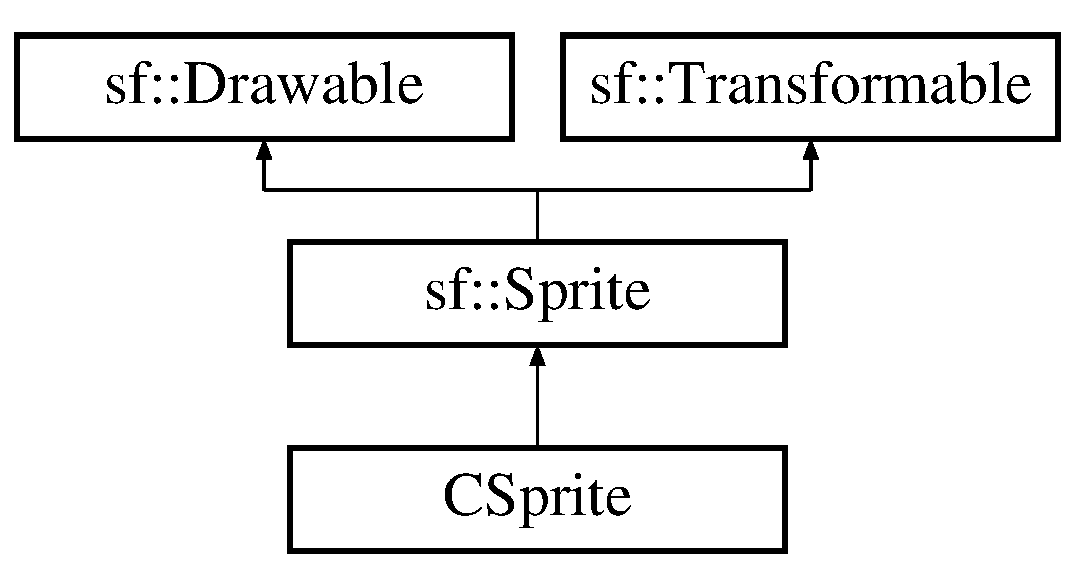
\includegraphics[height=3.000000cm]{classCSprite}
\end{center}
\end{figure}
\subsection*{Public Member Functions}
\begin{DoxyCompactItemize}
\item 
\hypertarget{classCSprite_afdfe7ac25b872dbafd60e6329185b0c5}{{\bfseries C\-Sprite} (\hyperlink{classCTexture}{C\-Texture} $\ast$p\-Texture, const \hyperlink{classsf_1_1Vector2}{sf\-::\-Vector2}$<$ int $>$ \&curr\-Sub)}\label{classCSprite_afdfe7ac25b872dbafd60e6329185b0c5}

\item 
\hypertarget{classCSprite_a7fa10fe45cf1683163671b7483ffc758}{{\bfseries C\-Sprite} (const \hyperlink{classCSprite}{C\-Sprite} \&other)}\label{classCSprite_a7fa10fe45cf1683163671b7483ffc758}

\item 
\hypertarget{classCSprite_a2162a3b87f87eecf9e9b93fe4c573690}{void {\bfseries set\-Sub\-Image} (int col, int row)}\label{classCSprite_a2162a3b87f87eecf9e9b93fe4c573690}

\item 
\hypertarget{classCSprite_a6e46dd766754438ebdefadf3449540da}{void {\bfseries set\-Sub\-Image} (const \hyperlink{classsf_1_1Vector2}{sf\-::\-Vector2}$<$ int $>$ $\ast$new\-Sub)}\label{classCSprite_a6e46dd766754438ebdefadf3449540da}

\end{DoxyCompactItemize}
\subsection*{Additional Inherited Members}


\subsection{Detailed Description}


Definition at line 14 of file C\-Sprite.\-h.



The documentation for this class was generated from the following files\-:\begin{DoxyCompactItemize}
\item 
/home/z\-Zelman/\-Dropbox/\-Placeholder-\/\-R\-T\-S/src/\-Graphics/C\-Sprite.\-h\item 
/home/z\-Zelman/\-Dropbox/\-Placeholder-\/\-R\-T\-S/src/\-Graphics/C\-Sprite.\-cpp\end{DoxyCompactItemize}

\hypertarget{classCTexture}{\section{C\-Texture Class Reference}
\label{classCTexture}\index{C\-Texture@{C\-Texture}}
}
Inheritance diagram for C\-Texture\-:\begin{figure}[H]
\begin{center}
\leavevmode
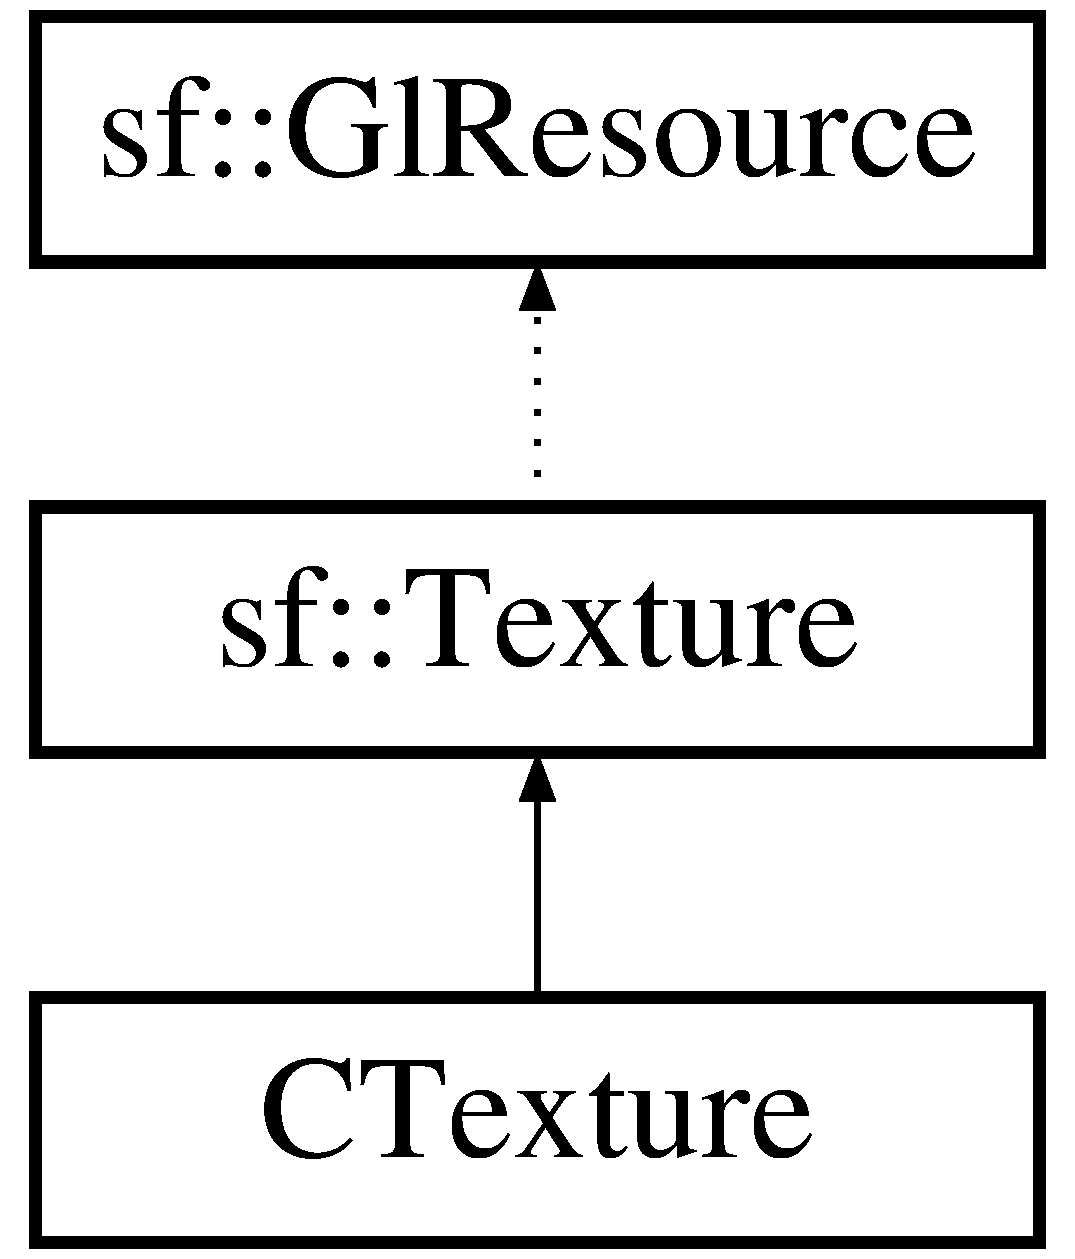
\includegraphics[height=3.000000cm]{classCTexture}
\end{center}
\end{figure}
\subsection*{Public Member Functions}
\begin{DoxyCompactItemize}
\item 
\hypertarget{classCTexture_a03a03314b328783682d200443b561890}{{\bfseries C\-Texture} (std\-::string file\-Name, const \hyperlink{classsf_1_1Vector2}{sf\-::\-Vector2}$<$ int $>$ \&sub\-Size, const \hyperlink{classsf_1_1Vector2}{sf\-::\-Vector2}$<$ int $>$ \&sub\-Num)}\label{classCTexture_a03a03314b328783682d200443b561890}

\item 
\hypertarget{classCTexture_a2bb6709e0d63ccb6fb3219eb5528570f}{{\bfseries C\-Texture} (const \hyperlink{classCTexture}{C\-Texture} \&other)}\label{classCTexture_a2bb6709e0d63ccb6fb3219eb5528570f}

\item 
\hypertarget{classCTexture_ab4f29f7f73e347dfac33672e3b9a64c8}{\hyperlink{classCTexture}{C\-Texture} \& {\bfseries operator=} (const \hyperlink{classCTexture}{C\-Texture} \&other)}\label{classCTexture_ab4f29f7f73e347dfac33672e3b9a64c8}

\item 
\hypertarget{classCTexture_a52a074211eaa812a91200f73f8387aca}{const \hyperlink{classsf_1_1Vector2}{sf\-::\-Vector2}$<$ int $>$ \& {\bfseries get\-Sub\-Num} () const }\label{classCTexture_a52a074211eaa812a91200f73f8387aca}

\item 
\hypertarget{classCTexture_a100f28379f113485d1e7574705ba977f}{const \hyperlink{classsf_1_1Vector2}{sf\-::\-Vector2}$<$ int $>$ \& {\bfseries get\-Sub\-Size} () const }\label{classCTexture_a100f28379f113485d1e7574705ba977f}

\item 
\hypertarget{classCTexture_a0756fcbdac0b2e53cbaea1c35c64a939}{void {\bfseries load} (std\-::string file\-Name)}\label{classCTexture_a0756fcbdac0b2e53cbaea1c35c64a939}

\end{DoxyCompactItemize}
\subsection*{Additional Inherited Members}


\subsection{Detailed Description}


Definition at line 13 of file C\-Texture.\-h.



The documentation for this class was generated from the following files\-:\begin{DoxyCompactItemize}
\item 
/home/z\-Zelman/\-Dropbox/\-Placeholder-\/\-R\-T\-S/src/\-Graphics/C\-Texture.\-h\item 
/home/z\-Zelman/\-Dropbox/\-Placeholder-\/\-R\-T\-S/src/\-Graphics/C\-Texture.\-cpp\end{DoxyCompactItemize}

\hypertarget{classCTile}{\section{C\-Tile Class Reference}
\label{classCTile}\index{C\-Tile@{C\-Tile}}
}
Inheritance diagram for C\-Tile\-:\begin{figure}[H]
\begin{center}
\leavevmode
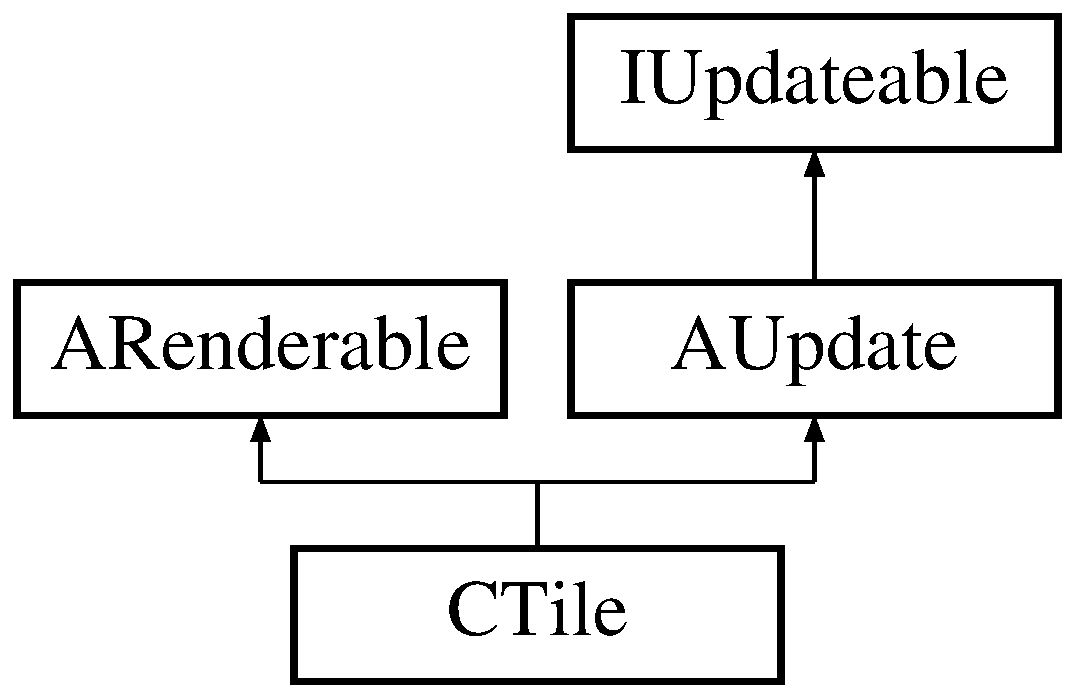
\includegraphics[height=3.000000cm]{classCTile}
\end{center}
\end{figure}
\subsection*{Public Member Functions}
\begin{DoxyCompactItemize}
\item 
\hypertarget{classCTile_a030eef2d18fb054c0fa6738784af0b0d}{{\bfseries C\-Tile} (\hyperlink{classCTexture}{C\-Texture} $\ast$p\-Texture, const \hyperlink{classsf_1_1Vector2}{sf\-::\-Vector2}$<$ int $>$ \&curr\-Sub)}\label{classCTile_a030eef2d18fb054c0fa6738784af0b0d}

\item 
\hypertarget{classCTile_a07c38be9c331480eb7c8d526b084a287}{{\bfseries C\-Tile} (\hyperlink{classCSprite}{C\-Sprite} $\ast$p\-Sprite)}\label{classCTile_a07c38be9c331480eb7c8d526b084a287}

\item 
\hypertarget{classCTile_a818a17e48a7219eedac950b82c641ee0}{void {\bfseries update} ()}\label{classCTile_a818a17e48a7219eedac950b82c641ee0}

\end{DoxyCompactItemize}
\subsection*{Additional Inherited Members}


\subsection{Detailed Description}


Definition at line 16 of file C\-Tile.\-h.



The documentation for this class was generated from the following files\-:\begin{DoxyCompactItemize}
\item 
/home/z\-Zelman/\-Dropbox/\-Placeholder-\/\-R\-T\-S/src/\-Tiles/C\-Tile.\-h\item 
/home/z\-Zelman/\-Dropbox/\-Placeholder-\/\-R\-T\-S/src/\-Tiles/C\-Tile.\-cpp\end{DoxyCompactItemize}

\hypertarget{classCTile__Container}{\section{C\-Tile\-\_\-\-Container Class Reference}
\label{classCTile__Container}\index{C\-Tile\-\_\-\-Container@{C\-Tile\-\_\-\-Container}}
}
Inheritance diagram for C\-Tile\-\_\-\-Container\-:\begin{figure}[H]
\begin{center}
\leavevmode
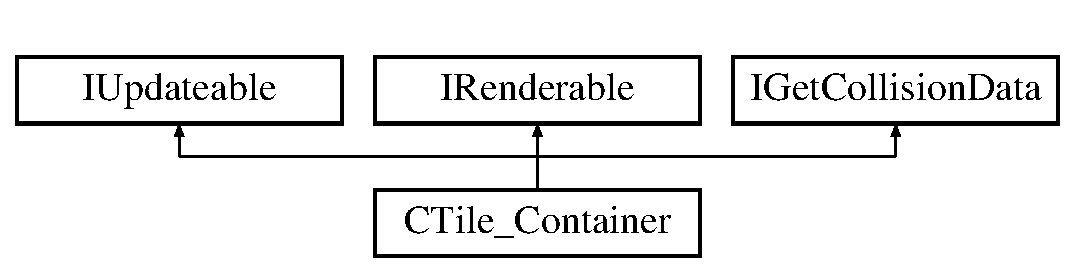
\includegraphics[height=2.000000cm]{classCTile__Container}
\end{center}
\end{figure}
\subsection*{Public Member Functions}
\begin{DoxyCompactItemize}
\item 
\hypertarget{classCTile__Container_ab3f79e82961b644d422874eb558ea312}{{\bfseries C\-Tile\-\_\-\-Container} (std\-::string file\-Name)}\label{classCTile__Container_ab3f79e82961b644d422874eb558ea312}

\item 
\hypertarget{classCTile__Container_ae8a4d2b6e49fbec47d92cbb19bb9d3c7}{\hyperlink{classsf_1_1Vector2}{sf\-::\-Vector2}$<$ int $>$ {\bfseries get\-Grid\-Size} ()}\label{classCTile__Container_ae8a4d2b6e49fbec47d92cbb19bb9d3c7}

\item 
\hypertarget{classCTile__Container_a876984278369d0cafc24890959128ed0}{\hyperlink{classsf_1_1Vector2}{sf\-::\-Vector2}$<$ int $>$ {\bfseries get\-Grid\-Sub\-Size} ()}\label{classCTile__Container_a876984278369d0cafc24890959128ed0}

\item 
\hypertarget{classCTile__Container_abe6e19de544f042671094697bb83fde9}{void {\bfseries update} ()}\label{classCTile__Container_abe6e19de544f042671094697bb83fde9}

\item 
\hypertarget{classCTile__Container_ae61b573ed7b47bea750040a26b492632}{void {\bfseries get\-Collisiondata} (std\-::list$<$ \hyperlink{classARenderable}{A\-Renderable} $\ast$ $>$ $\ast$p\-List)}\label{classCTile__Container_ae61b573ed7b47bea750040a26b492632}

\item 
\hypertarget{classCTile__Container_a48c74611efadee522595362a79620bff}{void {\bfseries get\-Render\-Data} (std\-::list$<$ \hyperlink{classARenderable}{A\-Renderable} $\ast$ $>$ $\ast$p\-List)}\label{classCTile__Container_a48c74611efadee522595362a79620bff}

\item 
\hypertarget{classCTile__Container_a14f90644c3a992813a629cea3e81aa38}{void {\bfseries screen\-To\-Grid} (int $\ast$pos\-X, int $\ast$pos\-Y)}\label{classCTile__Container_a14f90644c3a992813a629cea3e81aa38}

\item 
\hypertarget{classCTile__Container_adfda15836508531632c4ca506caf6360}{bool {\bfseries is\-Collision} (const \hyperlink{classsf_1_1Rect}{sf\-::\-Rect}$<$ float $>$ \&rect, \hyperlink{classCSprite}{C\-Sprite} $\ast$\&p\-Sprite)}\label{classCTile__Container_adfda15836508531632c4ca506caf6360}

\item 
\hypertarget{classCTile__Container_a4195d75fcc4790946b19ea82fc693a1c}{bool {\bfseries is\-Collision} (const \hyperlink{classsf_1_1Vector2}{sf\-::\-Vector2}$<$ float $>$ \&point, \hyperlink{classCSprite}{C\-Sprite} $\ast$\&p\-Sprite)}\label{classCTile__Container_a4195d75fcc4790946b19ea82fc693a1c}

\item 
\hypertarget{classCTile__Container_a3c8b4ccbb9afaaa9462a11962b6e2dbd}{bool {\bfseries is\-Collision} (float x, float y, \hyperlink{classCSprite}{C\-Sprite} $\ast$\&p\-Sprite)}\label{classCTile__Container_a3c8b4ccbb9afaaa9462a11962b6e2dbd}

\end{DoxyCompactItemize}


\subsection{Detailed Description}


Definition at line 23 of file C\-Tile\-\_\-\-Container.\-h.



The documentation for this class was generated from the following files\-:\begin{DoxyCompactItemize}
\item 
/home/z\-Zelman/\-Dropbox/\-Placeholder-\/\-R\-T\-S/src/\-Tiles/C\-Tile\-\_\-\-Container.\-h\item 
/home/z\-Zelman/\-Dropbox/\-Placeholder-\/\-R\-T\-S/src/\-Tiles/C\-Tile\-\_\-\-Container.\-cpp\end{DoxyCompactItemize}

\hypertarget{classCUI}{\section{C\-U\-I Class Reference}
\label{classCUI}\index{C\-U\-I@{C\-U\-I}}
}


{\ttfamily \#include $<$C\-U\-I.\-h$>$}

Inheritance diagram for C\-U\-I\-:\begin{figure}[H]
\begin{center}
\leavevmode
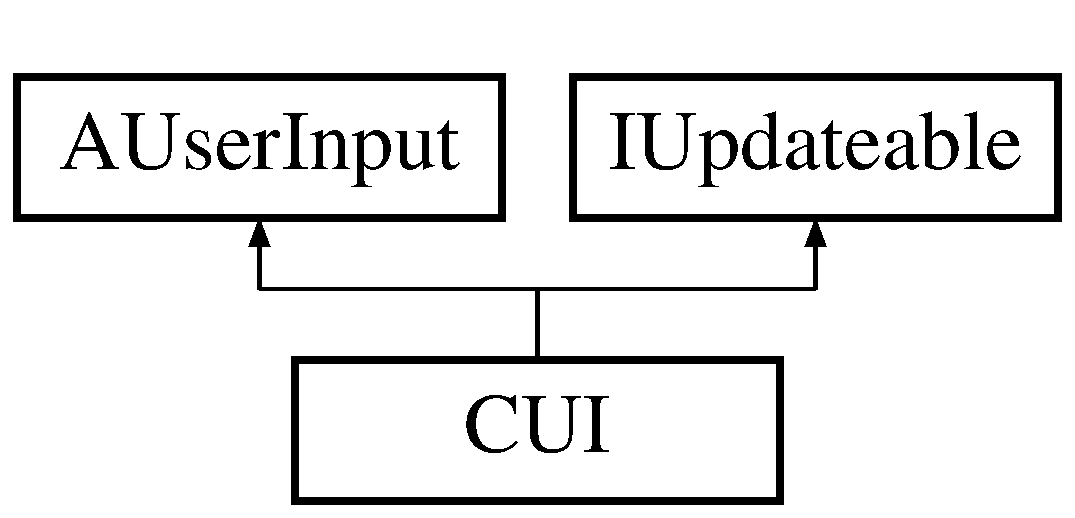
\includegraphics[height=2.000000cm]{classCUI}
\end{center}
\end{figure}
\subsection*{Public Member Functions}
\begin{DoxyCompactItemize}
\item 
\hypertarget{classCUI_a0332db7aa3a731b21009682464f3dcb8}{{\bfseries C\-U\-I} (\hyperlink{classCTile__Container}{C\-Tile\-\_\-\-Container} $\ast$p\-Tile\-\_\-\-Container, \hyperlink{classCRoom__Container}{C\-Room\-\_\-\-Container} $\ast$p\-Room\-\_\-\-Container, \hyperlink{classCSpawner}{C\-Spawner} $\ast$p\-Spawner)}\label{classCUI_a0332db7aa3a731b21009682464f3dcb8}

\item 
\hypertarget{classCUI_ab0b322040b41a6650bd625216f77b75c}{void {\bfseries update} ()}\label{classCUI_ab0b322040b41a6650bd625216f77b75c}

\item 
\hypertarget{classCUI_addb1531f20541cb7c7f8688f1cd843e9}{bool {\bfseries user\-Input\-\_\-key\-Press} (\hyperlink{classsf_1_1Event}{sf\-::\-Event} $\ast$p\-Event)}\label{classCUI_addb1531f20541cb7c7f8688f1cd843e9}

\item 
\hypertarget{classCUI_a0495bb6ad5fba9ef0552a487151f7896}{bool {\bfseries user\-Input\-\_\-key\-Release} (\hyperlink{classsf_1_1Event}{sf\-::\-Event} $\ast$p\-Event)}\label{classCUI_a0495bb6ad5fba9ef0552a487151f7896}

\item 
\hypertarget{classCUI_a6edfa48bb429f6e1468f5c3568cf83c5}{bool {\bfseries user\-Input\-\_\-mouse\-Press} (\hyperlink{classsf_1_1Event}{sf\-::\-Event} $\ast$p\-Event)}\label{classCUI_a6edfa48bb429f6e1468f5c3568cf83c5}

\item 
\hypertarget{classCUI_a64e3c8ad256e2d814e7112d201cb78ae}{bool {\bfseries user\-Input\-\_\-mouse\-Release} (\hyperlink{classsf_1_1Event}{sf\-::\-Event} $\ast$p\-Event)}\label{classCUI_a64e3c8ad256e2d814e7112d201cb78ae}

\end{DoxyCompactItemize}
\subsection*{Additional Inherited Members}


\subsection{Detailed Description}
'Parses' user events, as well as keeps Bookkeeping information on several user states.

Keeps bookkeeping information for the states of keys that are bound to spawn Rooms/\-Units

Tells the 'Spawner' module to spawn specific objects based on current values of the key states

Uses a finite state machine to determine how user events are interpreted (menu vs. game-\/play) 

Definition at line 35 of file C\-U\-I.\-h.



The documentation for this class was generated from the following files\-:\begin{DoxyCompactItemize}
\item 
/home/z\-Zelman/\-Dropbox/\-Placeholder-\/\-R\-T\-S/src/\-U\-I/C\-U\-I.\-h\item 
/home/z\-Zelman/\-Dropbox/\-Placeholder-\/\-R\-T\-S/src/\-U\-I/C\-U\-I.\-cpp\end{DoxyCompactItemize}

\hypertarget{classCUnit}{\section{C\-Unit Class Reference}
\label{classCUnit}\index{C\-Unit@{C\-Unit}}
}
Inheritance diagram for C\-Unit\-:\begin{figure}[H]
\begin{center}
\leavevmode
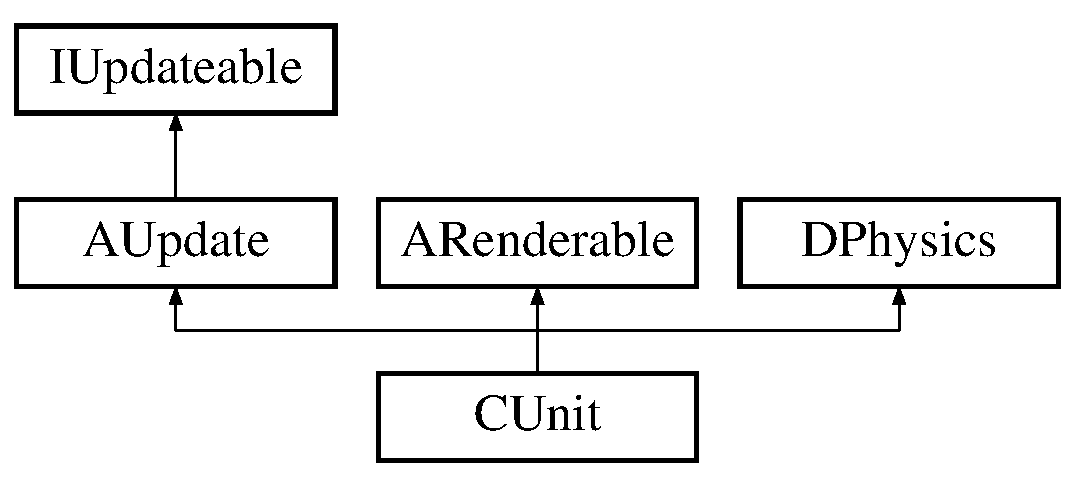
\includegraphics[height=3.000000cm]{classCUnit}
\end{center}
\end{figure}
\subsection*{Public Member Functions}
\begin{DoxyCompactItemize}
\item 
\hypertarget{classCUnit_ad438542eeeb73f398b526002e400cfc4}{{\bfseries C\-Unit} (\hyperlink{classCTile__Container}{C\-Tile\-\_\-\-Container} $\ast$p\-Grid, \hyperlink{classCTexture}{C\-Texture} $\ast$p\-Texture, const \hyperlink{classsf_1_1Vector2}{sf\-::\-Vector2}$<$ int $>$ \&curr\-Sub)}\label{classCUnit_ad438542eeeb73f398b526002e400cfc4}

\item 
\hypertarget{classCUnit_a8669992f78b1955874c14e66963f9752}{void {\bfseries update} ()}\label{classCUnit_a8669992f78b1955874c14e66963f9752}

\item 
\hypertarget{classCUnit_a3de88566a8ecfac18309859cf7282da2}{void {\bfseries step\-Normally} ()}\label{classCUnit_a3de88566a8ecfac18309859cf7282da2}

\end{DoxyCompactItemize}
\subsection*{Additional Inherited Members}


\subsection{Detailed Description}


Definition at line 18 of file C\-Unit.\-h.



The documentation for this class was generated from the following files\-:\begin{DoxyCompactItemize}
\item 
/home/z\-Zelman/\-Dropbox/\-Placeholder-\/\-R\-T\-S/src/\-Units/C\-Unit.\-h\item 
/home/z\-Zelman/\-Dropbox/\-Placeholder-\/\-R\-T\-S/src/\-Units/C\-Unit.\-cpp\end{DoxyCompactItemize}

\hypertarget{classCUnit__Container}{\section{C\-Unit\-\_\-\-Container Class Reference}
\label{classCUnit__Container}\index{C\-Unit\-\_\-\-Container@{C\-Unit\-\_\-\-Container}}
}
Inheritance diagram for C\-Unit\-\_\-\-Container\-:\begin{figure}[H]
\begin{center}
\leavevmode
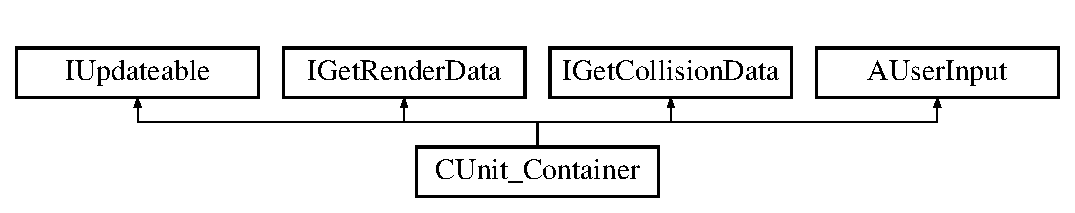
\includegraphics[height=2.000000cm]{classCUnit__Container}
\end{center}
\end{figure}
\subsection*{Public Member Functions}
\begin{DoxyCompactItemize}
\item 
\hypertarget{classCUnit__Container_a744405ccd2f0a8764d527e9d549b59ef}{{\bfseries C\-Unit\-\_\-\-Container} (\hyperlink{classsf_1_1RenderWindow}{sf\-::\-Render\-Window} $\ast$p\-Window, \hyperlink{classCTile__Container}{C\-Tile\-\_\-\-Container} $\ast$p\-Grid)}\label{classCUnit__Container_a744405ccd2f0a8764d527e9d549b59ef}

\item 
\hypertarget{classCUnit__Container_ac9f8730abcc32d9d1d98b32667e0df61}{void {\bfseries update} ()}\label{classCUnit__Container_ac9f8730abcc32d9d1d98b32667e0df61}

\item 
\hypertarget{classCUnit__Container_a681e14cd1a0745be8f454eff21a07c6b}{void {\bfseries render} ()}\label{classCUnit__Container_a681e14cd1a0745be8f454eff21a07c6b}

\item 
\hypertarget{classCUnit__Container_abe9cc4df18bbd9c60f76360c03b59627}{void {\bfseries get\-Collisiondata} (std\-::list$<$ \hyperlink{classARender}{A\-Render} $\ast$ $>$ $\ast$p\-List)}\label{classCUnit__Container_abe9cc4df18bbd9c60f76360c03b59627}

\item 
\hypertarget{classCUnit__Container_a83d19fd4d473972bc2720d571c6bfb73}{bool {\bfseries user\-Input\-\_\-key\-Press} (\hyperlink{classsf_1_1Event}{sf\-::\-Event} $\ast$p\-Event)}\label{classCUnit__Container_a83d19fd4d473972bc2720d571c6bfb73}

\item 
\hypertarget{classCUnit__Container_ad716ac99e85768e9da638fa971e7f5b0}{bool {\bfseries user\-Input\-\_\-key\-Release} (\hyperlink{classsf_1_1Event}{sf\-::\-Event} $\ast$p\-Event)}\label{classCUnit__Container_ad716ac99e85768e9da638fa971e7f5b0}

\item 
\hypertarget{classCUnit__Container_a2b3a12f90500e7b67413e772ece36cb2}{bool {\bfseries user\-Input\-\_\-mouse\-Press} (\hyperlink{classsf_1_1Event}{sf\-::\-Event} $\ast$p\-Event)}\label{classCUnit__Container_a2b3a12f90500e7b67413e772ece36cb2}

\item 
\hypertarget{classCUnit__Container_a3704686b7aecda14352236aed489fc25}{bool {\bfseries user\-Input\-\_\-mouse\-Release} (\hyperlink{classsf_1_1Event}{sf\-::\-Event} $\ast$p\-Event)}\label{classCUnit__Container_a3704686b7aecda14352236aed489fc25}

\end{DoxyCompactItemize}
\subsection*{Additional Inherited Members}


\subsection{Detailed Description}


Definition at line 21 of file C\-Unit\-\_\-\-Container.\-h.



The documentation for this class was generated from the following files\-:\begin{DoxyCompactItemize}
\item 
/home/z\-Zelman/\-Dropbox/\-Placeholder-\/\-R\-T\-S/src/\-Units/C\-Unit\-\_\-\-Container.\-h\item 
/home/z\-Zelman/\-Dropbox/\-Placeholder-\/\-R\-T\-S/src/\-Units/C\-Unit\-\_\-\-Container.\-cpp\end{DoxyCompactItemize}

\hypertarget{structsf_1_1Shader_1_1CurrentTextureType}{\section{sf\-:\-:Shader\-:\-:Current\-Texture\-Type Struct Reference}
\label{structsf_1_1Shader_1_1CurrentTextureType}\index{sf\-::\-Shader\-::\-Current\-Texture\-Type@{sf\-::\-Shader\-::\-Current\-Texture\-Type}}
}


Special type/value that can be passed to set\-Parameter, and that represents the texture of the object being drawn.  




{\ttfamily \#include $<$Shader.\-hpp$>$}



\subsection{Detailed Description}
Special type/value that can be passed to set\-Parameter, and that represents the texture of the object being drawn. 

Definition at line 70 of file Shader.\-hpp.



The documentation for this struct was generated from the following file\-:\begin{DoxyCompactItemize}
\item 
/home/z\-Zelman/\-Dropbox/\-Placeholder-\/\-R\-T\-S/\-S\-F\-M\-L-\/2.\-1/include/\-S\-F\-M\-L/\-Graphics/Shader.\-hpp\end{DoxyCompactItemize}

\hypertarget{classsf_1_1Ftp_1_1DirectoryResponse}{\section{sf\-:\-:Ftp\-:\-:Directory\-Response Class Reference}
\label{classsf_1_1Ftp_1_1DirectoryResponse}\index{sf\-::\-Ftp\-::\-Directory\-Response@{sf\-::\-Ftp\-::\-Directory\-Response}}
}


Specialization of F\-T\-P response returning a directory.  




{\ttfamily \#include $<$Ftp.\-hpp$>$}

Inheritance diagram for sf\-:\-:Ftp\-:\-:Directory\-Response\-:\begin{figure}[H]
\begin{center}
\leavevmode
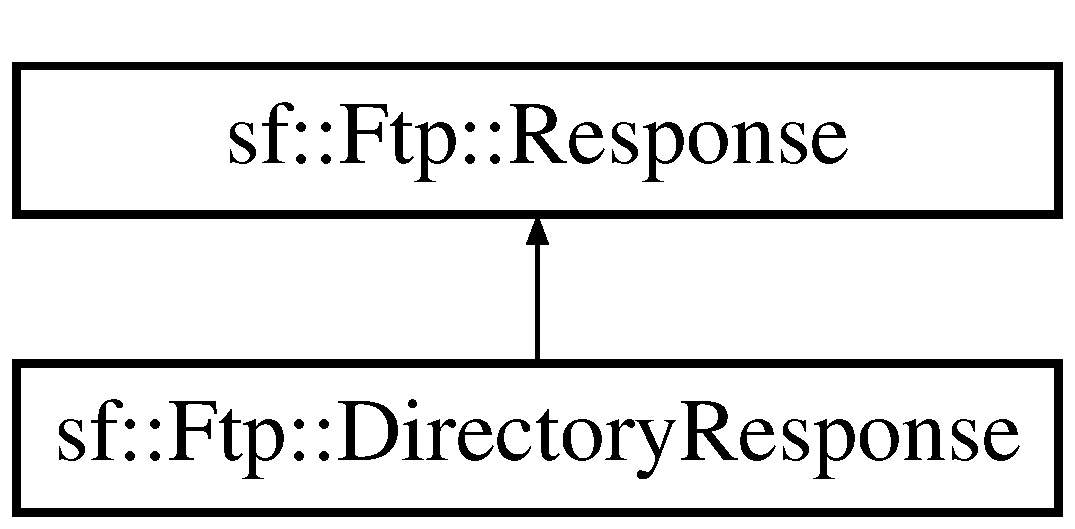
\includegraphics[height=2.000000cm]{classsf_1_1Ftp_1_1DirectoryResponse}
\end{center}
\end{figure}
\subsection*{Public Member Functions}
\begin{DoxyCompactItemize}
\item 
\hyperlink{classsf_1_1Ftp_1_1DirectoryResponse_a36b6d2728fa53c4ad37b7a6307f4d388}{Directory\-Response} (const \hyperlink{classsf_1_1Ftp_1_1Response}{Response} \&response)
\begin{DoxyCompactList}\small\item\em Default constructor. \end{DoxyCompactList}\item 
const std\-::string \& \hyperlink{classsf_1_1Ftp_1_1DirectoryResponse_a500793778ad0ed223aa86ed8fbee28a3}{get\-Directory} () const 
\begin{DoxyCompactList}\small\item\em Get the directory returned in the response. \end{DoxyCompactList}\end{DoxyCompactItemize}
\subsection*{Additional Inherited Members}


\subsection{Detailed Description}
Specialization of F\-T\-P response returning a directory. 

Definition at line 188 of file Ftp.\-hpp.



\subsection{Constructor \& Destructor Documentation}
\hypertarget{classsf_1_1Ftp_1_1DirectoryResponse_a36b6d2728fa53c4ad37b7a6307f4d388}{\index{sf\-::\-Ftp\-::\-Directory\-Response@{sf\-::\-Ftp\-::\-Directory\-Response}!Directory\-Response@{Directory\-Response}}
\index{Directory\-Response@{Directory\-Response}!sf::Ftp::DirectoryResponse@{sf\-::\-Ftp\-::\-Directory\-Response}}
\subsubsection[{Directory\-Response}]{\setlength{\rightskip}{0pt plus 5cm}sf\-::\-Ftp\-::\-Directory\-Response\-::\-Directory\-Response (
\begin{DoxyParamCaption}
\item[{const {\bf Response} \&}]{response}
\end{DoxyParamCaption}
)}}\label{classsf_1_1Ftp_1_1DirectoryResponse_a36b6d2728fa53c4ad37b7a6307f4d388}


Default constructor. 


\begin{DoxyParams}{Parameters}
{\em response} & Source response \\
\hline
\end{DoxyParams}


\subsection{Member Function Documentation}
\hypertarget{classsf_1_1Ftp_1_1DirectoryResponse_a500793778ad0ed223aa86ed8fbee28a3}{\index{sf\-::\-Ftp\-::\-Directory\-Response@{sf\-::\-Ftp\-::\-Directory\-Response}!get\-Directory@{get\-Directory}}
\index{get\-Directory@{get\-Directory}!sf::Ftp::DirectoryResponse@{sf\-::\-Ftp\-::\-Directory\-Response}}
\subsubsection[{get\-Directory}]{\setlength{\rightskip}{0pt plus 5cm}const std\-::string\& sf\-::\-Ftp\-::\-Directory\-Response\-::get\-Directory (
\begin{DoxyParamCaption}
{}
\end{DoxyParamCaption}
) const}}\label{classsf_1_1Ftp_1_1DirectoryResponse_a500793778ad0ed223aa86ed8fbee28a3}


Get the directory returned in the response. 

\begin{DoxyReturn}{Returns}
Directory name 
\end{DoxyReturn}


The documentation for this class was generated from the following file\-:\begin{DoxyCompactItemize}
\item 
/home/z\-Zelman/\-Dropbox/\-Placeholder-\/\-R\-T\-S/\-S\-F\-M\-L-\/2.\-1/include/\-S\-F\-M\-L/\-Network/Ftp.\-hpp\end{DoxyCompactItemize}

\hypertarget{classDPhysics}{\section{D\-Physics Class Reference}
\label{classDPhysics}\index{D\-Physics@{D\-Physics}}
}
Inheritance diagram for D\-Physics\-:\begin{figure}[H]
\begin{center}
\leavevmode
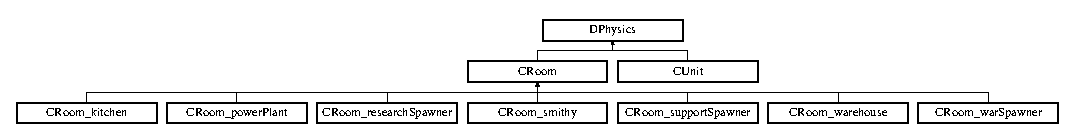
\includegraphics[height=1.428571cm]{classDPhysics}
\end{center}
\end{figure}
\subsection*{Classes}
\begin{DoxyCompactItemize}
\item 
struct \hyperlink{structDPhysics_1_1SPhysics}{S\-Physics}
\end{DoxyCompactItemize}
\subsection*{Public Member Functions}
\begin{DoxyCompactItemize}
\item 
\hypertarget{classDPhysics_a414316ffcec06dbf01ced086bbb92b55}{virtual void {\bfseries step\-Normally} ()=0}\label{classDPhysics_a414316ffcec06dbf01ced086bbb92b55}

\end{DoxyCompactItemize}
\subsection*{Public Attributes}
\begin{DoxyCompactItemize}
\item 
\hypertarget{classDPhysics_aca2940879481f0e2b892c82c5fc0da5a}{struct \hyperlink{structDPhysics_1_1SPhysics}{D\-Physics\-::\-S\-Physics} {\bfseries m\-\_\-s\-Physics}}\label{classDPhysics_aca2940879481f0e2b892c82c5fc0da5a}

\end{DoxyCompactItemize}


\subsection{Detailed Description}


Definition at line 13 of file D\-Physics.\-h.



The documentation for this class was generated from the following files\-:\begin{DoxyCompactItemize}
\item 
/home/z\-Zelman/\-Dropbox/\-Placeholder-\/\-R\-T\-S/src/\-Physics/D\-Physics.\-h\item 
/home/z\-Zelman/\-Dropbox/\-Placeholder-\/\-R\-T\-S/src/\-Physics/D\-Physics.\-cpp\end{DoxyCompactItemize}

\hypertarget{classsf_1_1Drawable}{\section{sf\-:\-:Drawable Class Reference}
\label{classsf_1_1Drawable}\index{sf\-::\-Drawable@{sf\-::\-Drawable}}
}


Abstract base class for objects that can be drawn to a render target.  




{\ttfamily \#include $<$Drawable.\-hpp$>$}

Inheritance diagram for sf\-:\-:Drawable\-:\begin{figure}[H]
\begin{center}
\leavevmode
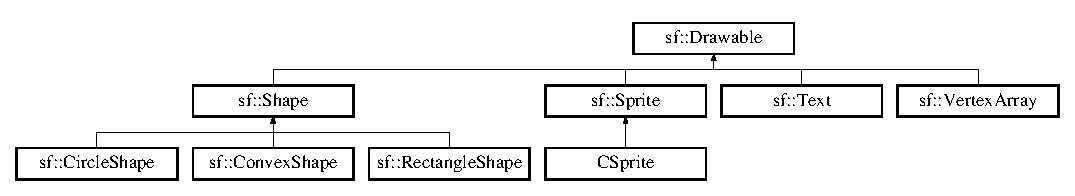
\includegraphics[height=2.187500cm]{classsf_1_1Drawable}
\end{center}
\end{figure}
\subsection*{Public Member Functions}
\begin{DoxyCompactItemize}
\item 
\hypertarget{classsf_1_1Drawable_a906002f2df7beb5edbddf5bbef96f120}{virtual \hyperlink{classsf_1_1Drawable_a906002f2df7beb5edbddf5bbef96f120}{$\sim$\-Drawable} ()}\label{classsf_1_1Drawable_a906002f2df7beb5edbddf5bbef96f120}

\begin{DoxyCompactList}\small\item\em Virtual destructor. \end{DoxyCompactList}\end{DoxyCompactItemize}
\subsection*{Protected Member Functions}
\begin{DoxyCompactItemize}
\item 
virtual void \hyperlink{classsf_1_1Drawable_a90d2c88bba9b035a0844eccb380ef631}{draw} (\hyperlink{classsf_1_1RenderTarget}{Render\-Target} \&target, \hyperlink{classsf_1_1RenderStates}{Render\-States} states) const =0
\begin{DoxyCompactList}\small\item\em Draw the object to a render target. \end{DoxyCompactList}\end{DoxyCompactItemize}
\subsection*{Friends}
\begin{DoxyCompactItemize}
\item 
\hypertarget{classsf_1_1Drawable_aa5afc6f82b7b587ed5ada4d227ce32aa}{class {\bfseries Render\-Target}}\label{classsf_1_1Drawable_aa5afc6f82b7b587ed5ada4d227ce32aa}

\end{DoxyCompactItemize}


\subsection{Detailed Description}
Abstract base class for objects that can be drawn to a render target. 

\hyperlink{classsf_1_1Drawable}{sf\-::\-Drawable} is a very simple base class that allows objects of derived classes to be drawn to a \hyperlink{classsf_1_1RenderTarget}{sf\-::\-Render\-Target}.

All you have to do in your derived class is to override the draw virtual function.

Note that inheriting from \hyperlink{classsf_1_1Drawable}{sf\-::\-Drawable} is not mandatory, but it allows this nice syntax \char`\"{}window.\-draw(object)\char`\"{} rather than \char`\"{}object.\-draw(window)\char`\"{}, which is more consistent with other S\-F\-M\-L classes.

Example\-: 
\begin{DoxyCode}
\textcolor{keyword}{class }MyDrawable : \textcolor{keyword}{public} \hyperlink{classsf_1_1Drawable}{sf::Drawable}
\{
\textcolor{keyword}{public} :

   ...

private :

    \textcolor{keyword}{virtual} \textcolor{keywordtype}{void} \hyperlink{classsf_1_1Drawable_a90d2c88bba9b035a0844eccb380ef631}{draw}(\hyperlink{classsf_1_1RenderTarget}{sf::RenderTarget}& target, 
      \hyperlink{classsf_1_1RenderStates}{sf::RenderStates} states)\textcolor{keyword}{ const}
\textcolor{keyword}{    }\{
        \textcolor{comment}{// You can draw other high-level objects}
        target.\hyperlink{classsf_1_1RenderTarget_a12417a3bcc245c41d957b29583556f39}{draw}(m\_sprite, states);

        \textcolor{comment}{// ... or use the low-level API}
        states.\hyperlink{classsf_1_1RenderStates_a457fc5a41731889de9cf39cf9b3436c3}{texture} = &m\_texture;
        target.\hyperlink{classsf_1_1RenderTarget_a12417a3bcc245c41d957b29583556f39}{draw}(m\_vertices, states);

        \textcolor{comment}{// ... or draw with OpenGL directly}
        glBegin(GL\_QUADS);
        ...
        glEnd();
    \}

    \hyperlink{classsf_1_1Sprite}{sf::Sprite} m\_sprite;
    \hyperlink{classsf_1_1Texture}{sf::Texture} m\_texture;
    \hyperlink{classsf_1_1VertexArray}{sf::VertexArray} m\_vertices;
\};
\end{DoxyCode}


\begin{DoxySeeAlso}{See Also}
\hyperlink{classsf_1_1RenderTarget}{sf\-::\-Render\-Target} 
\end{DoxySeeAlso}


Definition at line 44 of file Drawable.\-hpp.



\subsection{Member Function Documentation}
\hypertarget{classsf_1_1Drawable_a90d2c88bba9b035a0844eccb380ef631}{\index{sf\-::\-Drawable@{sf\-::\-Drawable}!draw@{draw}}
\index{draw@{draw}!sf::Drawable@{sf\-::\-Drawable}}
\subsubsection[{draw}]{\setlength{\rightskip}{0pt plus 5cm}virtual void sf\-::\-Drawable\-::draw (
\begin{DoxyParamCaption}
\item[{{\bf Render\-Target} \&}]{target, }
\item[{{\bf Render\-States}}]{states}
\end{DoxyParamCaption}
) const\hspace{0.3cm}{\ttfamily [protected]}, {\ttfamily [pure virtual]}}}\label{classsf_1_1Drawable_a90d2c88bba9b035a0844eccb380ef631}


Draw the object to a render target. 

This is a pure virtual function that has to be implemented by the derived class to define how the drawable should be drawn.


\begin{DoxyParams}{Parameters}
{\em target} & Render target to draw to \\
\hline
{\em states} & Current render states \\
\hline
\end{DoxyParams}


The documentation for this class was generated from the following file\-:\begin{DoxyCompactItemize}
\item 
/home/z\-Zelman/\-Dropbox/\-Placeholder-\/\-R\-T\-S/\-S\-F\-M\-L-\/2.\-1/include/\-S\-F\-M\-L/\-Graphics/Drawable.\-hpp\end{DoxyCompactItemize}

\hypertarget{classsf_1_1Event}{\section{sf\-:\-:Event Class Reference}
\label{classsf_1_1Event}\index{sf\-::\-Event@{sf\-::\-Event}}
}


Defines a system event and its parameters.  




{\ttfamily \#include $<$Event.\-hpp$>$}

\subsection*{Classes}
\begin{DoxyCompactItemize}
\item 
struct \hyperlink{structsf_1_1Event_1_1JoystickButtonEvent}{Joystick\-Button\-Event}
\begin{DoxyCompactList}\small\item\em \hyperlink{classsf_1_1Joystick}{Joystick} buttons events parameters (Joystick\-Button\-Pressed, Joystick\-Button\-Released) \end{DoxyCompactList}\item 
struct \hyperlink{structsf_1_1Event_1_1JoystickConnectEvent}{Joystick\-Connect\-Event}
\begin{DoxyCompactList}\small\item\em \hyperlink{classsf_1_1Joystick}{Joystick} connection events parameters (Joystick\-Connected, Joystick\-Disconnected) \end{DoxyCompactList}\item 
struct \hyperlink{structsf_1_1Event_1_1JoystickMoveEvent}{Joystick\-Move\-Event}
\begin{DoxyCompactList}\small\item\em \hyperlink{classsf_1_1Joystick}{Joystick} axis move event parameters (Joystick\-Moved) \end{DoxyCompactList}\item 
struct \hyperlink{structsf_1_1Event_1_1KeyEvent}{Key\-Event}
\begin{DoxyCompactList}\small\item\em \hyperlink{classsf_1_1Keyboard}{Keyboard} event parameters (Key\-Pressed, Key\-Released) \end{DoxyCompactList}\item 
struct \hyperlink{structsf_1_1Event_1_1MouseButtonEvent}{Mouse\-Button\-Event}
\begin{DoxyCompactList}\small\item\em \hyperlink{classsf_1_1Mouse}{Mouse} buttons events parameters (Mouse\-Button\-Pressed, Mouse\-Button\-Released) \end{DoxyCompactList}\item 
struct \hyperlink{structsf_1_1Event_1_1MouseMoveEvent}{Mouse\-Move\-Event}
\begin{DoxyCompactList}\small\item\em \hyperlink{classsf_1_1Mouse}{Mouse} move event parameters (Mouse\-Moved) \end{DoxyCompactList}\item 
struct \hyperlink{structsf_1_1Event_1_1MouseWheelEvent}{Mouse\-Wheel\-Event}
\begin{DoxyCompactList}\small\item\em \hyperlink{classsf_1_1Mouse}{Mouse} wheel events parameters (Mouse\-Wheel\-Moved) \end{DoxyCompactList}\item 
struct \hyperlink{structsf_1_1Event_1_1SizeEvent}{Size\-Event}
\begin{DoxyCompactList}\small\item\em Size events parameters (Resized) \end{DoxyCompactList}\item 
struct \hyperlink{structsf_1_1Event_1_1TextEvent}{Text\-Event}
\begin{DoxyCompactList}\small\item\em \hyperlink{classsf_1_1Text}{Text} event parameters (Text\-Entered) \end{DoxyCompactList}\end{DoxyCompactItemize}
\subsection*{Public Types}
\begin{DoxyCompactItemize}
\item 
enum \hyperlink{classsf_1_1Event_af41fa9ed45c02449030699f671331d4a}{Event\-Type} \{ \\*
\hyperlink{classsf_1_1Event_af41fa9ed45c02449030699f671331d4aa316e4212e083f1dce79efd8d9e9c0a95}{Closed}, 
\hyperlink{classsf_1_1Event_af41fa9ed45c02449030699f671331d4aa67fd26d7e520bc6722db3ff47ef24941}{Resized}, 
\hyperlink{classsf_1_1Event_af41fa9ed45c02449030699f671331d4aabd7877b5011a337268357c973e8347bd}{Lost\-Focus}, 
\hyperlink{classsf_1_1Event_af41fa9ed45c02449030699f671331d4aa8c5003ced508499933d540df8a6023ec}{Gained\-Focus}, 
\\*
\hyperlink{classsf_1_1Event_af41fa9ed45c02449030699f671331d4aa7e09871dc984080ff528e4f7e073e874}{Text\-Entered}, 
\hyperlink{classsf_1_1Event_af41fa9ed45c02449030699f671331d4aac3c7abfaa98c73bfe6be0b57df09c71b}{Key\-Pressed}, 
\hyperlink{classsf_1_1Event_af41fa9ed45c02449030699f671331d4aaa5bcc1e603d5a6f4c137af39558bd5d1}{Key\-Released}, 
\hyperlink{classsf_1_1Event_af41fa9ed45c02449030699f671331d4aa5cc9d3941af2a36049f4f9922c934a80}{Mouse\-Wheel\-Moved}, 
\\*
\hyperlink{classsf_1_1Event_af41fa9ed45c02449030699f671331d4aa55a3dcc8bf6c40e37f9ff2cdf606481f}{Mouse\-Button\-Pressed}, 
\hyperlink{classsf_1_1Event_af41fa9ed45c02449030699f671331d4aa9be69ecc07e484467ebbb133182fe5c1}{Mouse\-Button\-Released}, 
\hyperlink{classsf_1_1Event_af41fa9ed45c02449030699f671331d4aa4ff4fc3b3dc857e3617a63feb54be209}{Mouse\-Moved}, 
\hyperlink{classsf_1_1Event_af41fa9ed45c02449030699f671331d4aa50d98590a953e74c7ccf3dabadb22067}{Mouse\-Entered}, 
\\*
\hyperlink{classsf_1_1Event_af41fa9ed45c02449030699f671331d4aaa90b8526b328e0246d04b026de17c6e7}{Mouse\-Left}, 
\hyperlink{classsf_1_1Event_af41fa9ed45c02449030699f671331d4aa6d46855f0253f065689b69cd09437222}{Joystick\-Button\-Pressed}, 
\hyperlink{classsf_1_1Event_af41fa9ed45c02449030699f671331d4aa2246ef5ee33f7fa4b2a53f042ceeac3d}{Joystick\-Button\-Released}, 
\hyperlink{classsf_1_1Event_af41fa9ed45c02449030699f671331d4aa4d6ad228485c135967831be16ec074dd}{Joystick\-Moved}, 
\\*
\hyperlink{classsf_1_1Event_af41fa9ed45c02449030699f671331d4aaabb8877ec2f0c92904170deded09321e}{Joystick\-Connected}, 
\hyperlink{classsf_1_1Event_af41fa9ed45c02449030699f671331d4aab6e161dab7abaf154cc1c7b554558cb6}{Joystick\-Disconnected}, 
\hyperlink{classsf_1_1Event_af41fa9ed45c02449030699f671331d4aae51749211243cab2ab270b29cdc32a70}{Count}
 \}
\begin{DoxyCompactList}\small\item\em Enumeration of the different types of events. \end{DoxyCompactList}\end{DoxyCompactItemize}
\subsection*{Public Attributes}
\begin{DoxyCompactItemize}
\item 
\hypertarget{classsf_1_1Event_adf2f8044f713fd9d6019077b0d1ffe0a}{\hyperlink{classsf_1_1Event_af41fa9ed45c02449030699f671331d4a}{Event\-Type} \hyperlink{classsf_1_1Event_adf2f8044f713fd9d6019077b0d1ffe0a}{type}}\label{classsf_1_1Event_adf2f8044f713fd9d6019077b0d1ffe0a}

\begin{DoxyCompactList}\small\item\em Type of the event. \end{DoxyCompactList}\item 
\hypertarget{classsf_1_1Event_a41262e8d65fd95c51c7cabbc7bde371b}{\begin{tabbing}
xx\=xx\=xx\=xx\=xx\=xx\=xx\=xx\=xx\=\kill
union \{\\
\>\hyperlink{structsf_1_1Event_1_1SizeEvent}{SizeEvent} \hyperlink{classsf_1_1Event_a85dae56a377eeffd39183c3f6fc96cb9}{size}\\
\>\>{\em Size event parameters (\hyperlink{classsf_1_1Event_af41fa9ed45c02449030699f671331d4aa67fd26d7e520bc6722db3ff47ef24941}{Event::Resized}) }\\
\>\hyperlink{structsf_1_1Event_1_1KeyEvent}{KeyEvent} \hyperlink{classsf_1_1Event_a45b92fc6757ca7c193f06b302e424ab0}{key}\\
\>\>{\em Key event parameters (\hyperlink{classsf_1_1Event_af41fa9ed45c02449030699f671331d4aac3c7abfaa98c73bfe6be0b57df09c71b}{Event::KeyPressed}, \hyperlink{classsf_1_1Event_af41fa9ed45c02449030699f671331d4aaa5bcc1e603d5a6f4c137af39558bd5d1}{Event::KeyReleased}) }\\
\>\hyperlink{structsf_1_1Event_1_1TextEvent}{TextEvent} \hyperlink{classsf_1_1Event_a00c7bba6bee892791847ec22440e0a83}{text}\\
\>\>{\em \hyperlink{classsf_1_1Text}{Text} event parameters (\hyperlink{classsf_1_1Event_af41fa9ed45c02449030699f671331d4aa7e09871dc984080ff528e4f7e073e874}{Event::TextEntered}) }\\
\>\hyperlink{structsf_1_1Event_1_1MouseMoveEvent}{MouseMoveEvent} \hyperlink{classsf_1_1Event_a786620ec4315d40c7c4cf4ddf3a1881f}{mouseMove}\\
\>\>{\em \hyperlink{classsf_1_1Mouse}{Mouse} move event parameters (\hyperlink{classsf_1_1Event_af41fa9ed45c02449030699f671331d4aa4ff4fc3b3dc857e3617a63feb54be209}{Event::MouseMoved}) }\\
\>\hyperlink{structsf_1_1Event_1_1MouseButtonEvent}{MouseButtonEvent} \hyperlink{classsf_1_1Event_a20886a16ab7624de070b97145bb1dcac}{mouseButton}\\
\>\>{\em \hyperlink{classsf_1_1Mouse}{Mouse} button event parameters (\hyperlink{classsf_1_1Event_af41fa9ed45c02449030699f671331d4aa55a3dcc8bf6c40e37f9ff2cdf606481f}{Event::MouseButtonPressed}, \hyperlink{classsf_1_1Event_af41fa9ed45c02449030699f671331d4aa9be69ecc07e484467ebbb133182fe5c1}{Event::MouseButtonReleased}) }\\
\>\hyperlink{structsf_1_1Event_1_1MouseWheelEvent}{MouseWheelEvent} \hyperlink{classsf_1_1Event_a8758c6d7998757978fd9146099a02a1e}{mouseWheel}\\
\>\>{\em \hyperlink{classsf_1_1Mouse}{Mouse} wheel event parameters (\hyperlink{classsf_1_1Event_af41fa9ed45c02449030699f671331d4aa5cc9d3941af2a36049f4f9922c934a80}{Event::MouseWheelMoved}) }\\
\>\hyperlink{structsf_1_1Event_1_1JoystickMoveEvent}{JoystickMoveEvent} \hyperlink{classsf_1_1Event_ac479e8351cc2024d5c1094dc33970f7f}{joystickMove}\\
\>\>{\em \hyperlink{classsf_1_1Joystick}{Joystick} move event parameters (\hyperlink{classsf_1_1Event_af41fa9ed45c02449030699f671331d4aa4d6ad228485c135967831be16ec074dd}{Event::JoystickMoved}) }\\
\>\hyperlink{structsf_1_1Event_1_1JoystickButtonEvent}{JoystickButtonEvent} \hyperlink{classsf_1_1Event_a42aad27a054c1c05bd5c3d020e1db174}{joystickButton}\\
\>\>{\em \hyperlink{classsf_1_1Joystick}{Joystick} button event parameters (\hyperlink{classsf_1_1Event_af41fa9ed45c02449030699f671331d4aa6d46855f0253f065689b69cd09437222}{Event::JoystickButtonPressed}, \hyperlink{classsf_1_1Event_af41fa9ed45c02449030699f671331d4aa2246ef5ee33f7fa4b2a53f042ceeac3d}{Event::JoystickButtonReleased}) }\\
\>\hyperlink{structsf_1_1Event_1_1JoystickConnectEvent}{JoystickConnectEvent} \hyperlink{classsf_1_1Event_aa354335c9ad73362442bc54ffe81118f}{joystickConnect}\\
\>\>{\em \hyperlink{classsf_1_1Joystick}{Joystick} (dis)connect event parameters (\hyperlink{classsf_1_1Event_af41fa9ed45c02449030699f671331d4aaabb8877ec2f0c92904170deded09321e}{Event::JoystickConnected}, \hyperlink{classsf_1_1Event_af41fa9ed45c02449030699f671331d4aab6e161dab7abaf154cc1c7b554558cb6}{Event::JoystickDisconnected}) }\\
\}; }\label{classsf_1_1Event_a41262e8d65fd95c51c7cabbc7bde371b}
\\

\end{tabbing}\end{DoxyCompactItemize}


\subsection{Detailed Description}
Defines a system event and its parameters. 

\hyperlink{classsf_1_1Event}{sf\-::\-Event} holds all the informations about a system event that just happened. Events are retrieved using the \hyperlink{classsf_1_1Window_a338e996585faf82e93069858e3b531b7}{sf\-::\-Window\-::poll\-Event} and \hyperlink{classsf_1_1Window_aaf02ab64fbc1d374eef3696df54137bc}{sf\-::\-Window\-::wait\-Event} functions.

A \hyperlink{classsf_1_1Event}{sf\-::\-Event} instance contains the type of the event (mouse moved, key pressed, window closed, ...) as well as the details about this particular event. Please note that the event parameters are defined in a union, which means that only the member matching the type of the event will be properly filled; all other members will have undefined values and must not be read if the type of the event doesn't match. For example, if you received a Key\-Pressed event, then you must read the event.\-key member, all other members such as event.\-Mouse\-Move or event.\-text will have undefined values.

Usage example\-: 
\begin{DoxyCode}
\hyperlink{classsf_1_1Event}{sf::Event} event;
\textcolor{keywordflow}{while} (window.\hyperlink{classsf_1_1Window_a338e996585faf82e93069858e3b531b7}{pollEvent}(event))
\{
    \textcolor{comment}{// Request for closing the window}
    \textcolor{keywordflow}{if} (event.\hyperlink{classsf_1_1Event_adf2f8044f713fd9d6019077b0d1ffe0a}{type} == \hyperlink{classsf_1_1Event_af41fa9ed45c02449030699f671331d4aa316e4212e083f1dce79efd8d9e9c0a95}{sf::Event::Closed})
        window.\hyperlink{classsf_1_1Window_a99d1e030387b0c26f5995670504fe7b5}{close}();

    \textcolor{comment}{// The escape key was pressed}
    \textcolor{keywordflow}{if} ((event.\hyperlink{classsf_1_1Event_adf2f8044f713fd9d6019077b0d1ffe0a}{type} == \hyperlink{classsf_1_1Event_af41fa9ed45c02449030699f671331d4aac3c7abfaa98c73bfe6be0b57df09c71b}{sf::Event::KeyPressed}) && (event.
      \hyperlink{classsf_1_1Event_a45b92fc6757ca7c193f06b302e424ab0}{key}.\hyperlink{structsf_1_1Event_1_1KeyEvent_a2879fdab8a68cb1c6ecc45730a2d0e61}{code} == \hyperlink{classsf_1_1Keyboard_acb4cacd7cc5802dec45724cf3314a142a64b7ecb543c5d03bec8383dde123c95d}{sf::Keyboard::Escape}))
        window.\hyperlink{classsf_1_1Window_a99d1e030387b0c26f5995670504fe7b5}{close}();

    \textcolor{comment}{// The window was resized}
    \textcolor{keywordflow}{if} (event.\hyperlink{classsf_1_1Event_adf2f8044f713fd9d6019077b0d1ffe0a}{type} == \hyperlink{classsf_1_1Event_af41fa9ed45c02449030699f671331d4aa67fd26d7e520bc6722db3ff47ef24941}{sf::Event::Resized})
        doSomethingWithTheNewSize(event.\hyperlink{classsf_1_1Event_a85dae56a377eeffd39183c3f6fc96cb9}{size}.\hyperlink{structsf_1_1Event_1_1SizeEvent_a20ea1b78c9bb1604432f8f0067bbfd94}{width}, event.\hyperlink{classsf_1_1Event_a85dae56a377eeffd39183c3f6fc96cb9}{size}.
      \hyperlink{structsf_1_1Event_1_1SizeEvent_af0f76a599d5f48189cb8d78d4e5facdb}{height});

    \textcolor{comment}{// etc ...}
\}
\end{DoxyCode}
 

Definition at line 43 of file Event.\-hpp.



\subsection{Member Enumeration Documentation}
\hypertarget{classsf_1_1Event_af41fa9ed45c02449030699f671331d4a}{\index{sf\-::\-Event@{sf\-::\-Event}!Event\-Type@{Event\-Type}}
\index{Event\-Type@{Event\-Type}!sf::Event@{sf\-::\-Event}}
\subsubsection[{Event\-Type}]{\setlength{\rightskip}{0pt plus 5cm}enum {\bf sf\-::\-Event\-::\-Event\-Type}}}\label{classsf_1_1Event_af41fa9ed45c02449030699f671331d4a}


Enumeration of the different types of events. 

\begin{Desc}
\item[Enumerator]\par
\begin{description}
\index{Closed@{Closed}!sf\-::\-Event@{sf\-::\-Event}}\index{sf\-::\-Event@{sf\-::\-Event}!Closed@{Closed}}\item[{\em 
\hypertarget{classsf_1_1Event_af41fa9ed45c02449030699f671331d4aa316e4212e083f1dce79efd8d9e9c0a95}{Closed}\label{classsf_1_1Event_af41fa9ed45c02449030699f671331d4aa316e4212e083f1dce79efd8d9e9c0a95}
}]The window requested to be closed (no data) \index{Resized@{Resized}!sf\-::\-Event@{sf\-::\-Event}}\index{sf\-::\-Event@{sf\-::\-Event}!Resized@{Resized}}\item[{\em 
\hypertarget{classsf_1_1Event_af41fa9ed45c02449030699f671331d4aa67fd26d7e520bc6722db3ff47ef24941}{Resized}\label{classsf_1_1Event_af41fa9ed45c02449030699f671331d4aa67fd26d7e520bc6722db3ff47ef24941}
}]The window was resized (data in event.\-size) \index{Lost\-Focus@{Lost\-Focus}!sf\-::\-Event@{sf\-::\-Event}}\index{sf\-::\-Event@{sf\-::\-Event}!Lost\-Focus@{Lost\-Focus}}\item[{\em 
\hypertarget{classsf_1_1Event_af41fa9ed45c02449030699f671331d4aabd7877b5011a337268357c973e8347bd}{Lost\-Focus}\label{classsf_1_1Event_af41fa9ed45c02449030699f671331d4aabd7877b5011a337268357c973e8347bd}
}]The window lost the focus (no data) \index{Gained\-Focus@{Gained\-Focus}!sf\-::\-Event@{sf\-::\-Event}}\index{sf\-::\-Event@{sf\-::\-Event}!Gained\-Focus@{Gained\-Focus}}\item[{\em 
\hypertarget{classsf_1_1Event_af41fa9ed45c02449030699f671331d4aa8c5003ced508499933d540df8a6023ec}{Gained\-Focus}\label{classsf_1_1Event_af41fa9ed45c02449030699f671331d4aa8c5003ced508499933d540df8a6023ec}
}]The window gained the focus (no data) \index{Text\-Entered@{Text\-Entered}!sf\-::\-Event@{sf\-::\-Event}}\index{sf\-::\-Event@{sf\-::\-Event}!Text\-Entered@{Text\-Entered}}\item[{\em 
\hypertarget{classsf_1_1Event_af41fa9ed45c02449030699f671331d4aa7e09871dc984080ff528e4f7e073e874}{Text\-Entered}\label{classsf_1_1Event_af41fa9ed45c02449030699f671331d4aa7e09871dc984080ff528e4f7e073e874}
}]A character was entered (data in event.\-text) \index{Key\-Pressed@{Key\-Pressed}!sf\-::\-Event@{sf\-::\-Event}}\index{sf\-::\-Event@{sf\-::\-Event}!Key\-Pressed@{Key\-Pressed}}\item[{\em 
\hypertarget{classsf_1_1Event_af41fa9ed45c02449030699f671331d4aac3c7abfaa98c73bfe6be0b57df09c71b}{Key\-Pressed}\label{classsf_1_1Event_af41fa9ed45c02449030699f671331d4aac3c7abfaa98c73bfe6be0b57df09c71b}
}]A key was pressed (data in event.\-key) \index{Key\-Released@{Key\-Released}!sf\-::\-Event@{sf\-::\-Event}}\index{sf\-::\-Event@{sf\-::\-Event}!Key\-Released@{Key\-Released}}\item[{\em 
\hypertarget{classsf_1_1Event_af41fa9ed45c02449030699f671331d4aaa5bcc1e603d5a6f4c137af39558bd5d1}{Key\-Released}\label{classsf_1_1Event_af41fa9ed45c02449030699f671331d4aaa5bcc1e603d5a6f4c137af39558bd5d1}
}]A key was released (data in event.\-key) \index{Mouse\-Wheel\-Moved@{Mouse\-Wheel\-Moved}!sf\-::\-Event@{sf\-::\-Event}}\index{sf\-::\-Event@{sf\-::\-Event}!Mouse\-Wheel\-Moved@{Mouse\-Wheel\-Moved}}\item[{\em 
\hypertarget{classsf_1_1Event_af41fa9ed45c02449030699f671331d4aa5cc9d3941af2a36049f4f9922c934a80}{Mouse\-Wheel\-Moved}\label{classsf_1_1Event_af41fa9ed45c02449030699f671331d4aa5cc9d3941af2a36049f4f9922c934a80}
}]The mouse wheel was scrolled (data in event.\-mouse\-Wheel) \index{Mouse\-Button\-Pressed@{Mouse\-Button\-Pressed}!sf\-::\-Event@{sf\-::\-Event}}\index{sf\-::\-Event@{sf\-::\-Event}!Mouse\-Button\-Pressed@{Mouse\-Button\-Pressed}}\item[{\em 
\hypertarget{classsf_1_1Event_af41fa9ed45c02449030699f671331d4aa55a3dcc8bf6c40e37f9ff2cdf606481f}{Mouse\-Button\-Pressed}\label{classsf_1_1Event_af41fa9ed45c02449030699f671331d4aa55a3dcc8bf6c40e37f9ff2cdf606481f}
}]A mouse button was pressed (data in event.\-mouse\-Button) \index{Mouse\-Button\-Released@{Mouse\-Button\-Released}!sf\-::\-Event@{sf\-::\-Event}}\index{sf\-::\-Event@{sf\-::\-Event}!Mouse\-Button\-Released@{Mouse\-Button\-Released}}\item[{\em 
\hypertarget{classsf_1_1Event_af41fa9ed45c02449030699f671331d4aa9be69ecc07e484467ebbb133182fe5c1}{Mouse\-Button\-Released}\label{classsf_1_1Event_af41fa9ed45c02449030699f671331d4aa9be69ecc07e484467ebbb133182fe5c1}
}]A mouse button was released (data in event.\-mouse\-Button) \index{Mouse\-Moved@{Mouse\-Moved}!sf\-::\-Event@{sf\-::\-Event}}\index{sf\-::\-Event@{sf\-::\-Event}!Mouse\-Moved@{Mouse\-Moved}}\item[{\em 
\hypertarget{classsf_1_1Event_af41fa9ed45c02449030699f671331d4aa4ff4fc3b3dc857e3617a63feb54be209}{Mouse\-Moved}\label{classsf_1_1Event_af41fa9ed45c02449030699f671331d4aa4ff4fc3b3dc857e3617a63feb54be209}
}]The mouse cursor moved (data in event.\-mouse\-Move) \index{Mouse\-Entered@{Mouse\-Entered}!sf\-::\-Event@{sf\-::\-Event}}\index{sf\-::\-Event@{sf\-::\-Event}!Mouse\-Entered@{Mouse\-Entered}}\item[{\em 
\hypertarget{classsf_1_1Event_af41fa9ed45c02449030699f671331d4aa50d98590a953e74c7ccf3dabadb22067}{Mouse\-Entered}\label{classsf_1_1Event_af41fa9ed45c02449030699f671331d4aa50d98590a953e74c7ccf3dabadb22067}
}]The mouse cursor entered the area of the window (no data) \index{Mouse\-Left@{Mouse\-Left}!sf\-::\-Event@{sf\-::\-Event}}\index{sf\-::\-Event@{sf\-::\-Event}!Mouse\-Left@{Mouse\-Left}}\item[{\em 
\hypertarget{classsf_1_1Event_af41fa9ed45c02449030699f671331d4aaa90b8526b328e0246d04b026de17c6e7}{Mouse\-Left}\label{classsf_1_1Event_af41fa9ed45c02449030699f671331d4aaa90b8526b328e0246d04b026de17c6e7}
}]The mouse cursor left the area of the window (no data) \index{Joystick\-Button\-Pressed@{Joystick\-Button\-Pressed}!sf\-::\-Event@{sf\-::\-Event}}\index{sf\-::\-Event@{sf\-::\-Event}!Joystick\-Button\-Pressed@{Joystick\-Button\-Pressed}}\item[{\em 
\hypertarget{classsf_1_1Event_af41fa9ed45c02449030699f671331d4aa6d46855f0253f065689b69cd09437222}{Joystick\-Button\-Pressed}\label{classsf_1_1Event_af41fa9ed45c02449030699f671331d4aa6d46855f0253f065689b69cd09437222}
}]A joystick button was pressed (data in event.\-joystick\-Button) \index{Joystick\-Button\-Released@{Joystick\-Button\-Released}!sf\-::\-Event@{sf\-::\-Event}}\index{sf\-::\-Event@{sf\-::\-Event}!Joystick\-Button\-Released@{Joystick\-Button\-Released}}\item[{\em 
\hypertarget{classsf_1_1Event_af41fa9ed45c02449030699f671331d4aa2246ef5ee33f7fa4b2a53f042ceeac3d}{Joystick\-Button\-Released}\label{classsf_1_1Event_af41fa9ed45c02449030699f671331d4aa2246ef5ee33f7fa4b2a53f042ceeac3d}
}]A joystick button was released (data in event.\-joystick\-Button) \index{Joystick\-Moved@{Joystick\-Moved}!sf\-::\-Event@{sf\-::\-Event}}\index{sf\-::\-Event@{sf\-::\-Event}!Joystick\-Moved@{Joystick\-Moved}}\item[{\em 
\hypertarget{classsf_1_1Event_af41fa9ed45c02449030699f671331d4aa4d6ad228485c135967831be16ec074dd}{Joystick\-Moved}\label{classsf_1_1Event_af41fa9ed45c02449030699f671331d4aa4d6ad228485c135967831be16ec074dd}
}]The joystick moved along an axis (data in event.\-joystick\-Move) \index{Joystick\-Connected@{Joystick\-Connected}!sf\-::\-Event@{sf\-::\-Event}}\index{sf\-::\-Event@{sf\-::\-Event}!Joystick\-Connected@{Joystick\-Connected}}\item[{\em 
\hypertarget{classsf_1_1Event_af41fa9ed45c02449030699f671331d4aaabb8877ec2f0c92904170deded09321e}{Joystick\-Connected}\label{classsf_1_1Event_af41fa9ed45c02449030699f671331d4aaabb8877ec2f0c92904170deded09321e}
}]A joystick was connected (data in event.\-joystick\-Connect) \index{Joystick\-Disconnected@{Joystick\-Disconnected}!sf\-::\-Event@{sf\-::\-Event}}\index{sf\-::\-Event@{sf\-::\-Event}!Joystick\-Disconnected@{Joystick\-Disconnected}}\item[{\em 
\hypertarget{classsf_1_1Event_af41fa9ed45c02449030699f671331d4aab6e161dab7abaf154cc1c7b554558cb6}{Joystick\-Disconnected}\label{classsf_1_1Event_af41fa9ed45c02449030699f671331d4aab6e161dab7abaf154cc1c7b554558cb6}
}]A joystick was disconnected (data in event.\-joystick\-Connect) \index{Count@{Count}!sf\-::\-Event@{sf\-::\-Event}}\index{sf\-::\-Event@{sf\-::\-Event}!Count@{Count}}\item[{\em 
\hypertarget{classsf_1_1Event_af41fa9ed45c02449030699f671331d4aae51749211243cab2ab270b29cdc32a70}{Count}\label{classsf_1_1Event_af41fa9ed45c02449030699f671331d4aae51749211243cab2ab270b29cdc32a70}
}]Keep last -- the total number of event types. \end{description}
\end{Desc}


Definition at line 148 of file Event.\-hpp.



The documentation for this class was generated from the following file\-:\begin{DoxyCompactItemize}
\item 
/home/z\-Zelman/\-Dropbox/\-Placeholder-\/\-R\-T\-S/\-S\-F\-M\-L-\/2.\-1/include/\-S\-F\-M\-L/\-Window/Event.\-hpp\end{DoxyCompactItemize}

\hypertarget{classrapidxml_1_1file}{\section{rapidxml\-:\-:file$<$ Ch $>$ Class Template Reference}
\label{classrapidxml_1_1file}\index{rapidxml\-::file$<$ Ch $>$@{rapidxml\-::file$<$ Ch $>$}}
}


Represents data loaded from a file.  




{\ttfamily \#include $<$rapidxml\-\_\-utils.\-hpp$>$}

\subsection*{Public Member Functions}
\begin{DoxyCompactItemize}
\item 
\hyperlink{classrapidxml_1_1file_ae881a3cab1fe7152d45c92a8d7606cb3}{file} (const char $\ast$filename)
\item 
\hyperlink{classrapidxml_1_1file_a90707ccd991cc392dcf4bef37eed9d1f}{file} (std\-::basic\-\_\-istream$<$ Ch $>$ \&stream)
\item 
Ch $\ast$ \hyperlink{classrapidxml_1_1file_af1c71d65862c7af14e4708e32a80c1de}{data} ()
\item 
const Ch $\ast$ \hyperlink{classrapidxml_1_1file_aceb8f5ebd577c946a74b1ea3e2e0c576}{data} () const 
\item 
std\-::size\-\_\-t \hyperlink{classrapidxml_1_1file_a20191d167c6e00a88a44ca9a3a54e1c5}{size} () const 
\end{DoxyCompactItemize}


\subsection{Detailed Description}
\subsubsection*{template$<$class Ch = char$>$class rapidxml\-::file$<$ Ch $>$}

Represents data loaded from a file. 

Definition at line 21 of file rapidxml\-\_\-utils.\-hpp.



\subsection{Constructor \& Destructor Documentation}
\hypertarget{classrapidxml_1_1file_ae881a3cab1fe7152d45c92a8d7606cb3}{\index{rapidxml\-::file@{rapidxml\-::file}!file@{file}}
\index{file@{file}!rapidxml::file@{rapidxml\-::file}}
\subsubsection[{file}]{\setlength{\rightskip}{0pt plus 5cm}template$<$class Ch = char$>$ {\bf rapidxml\-::file}$<$ Ch $>$\-::{\bf file} (
\begin{DoxyParamCaption}
\item[{const char $\ast$}]{filename}
\end{DoxyParamCaption}
)\hspace{0.3cm}{\ttfamily [inline]}}}\label{classrapidxml_1_1file_ae881a3cab1fe7152d45c92a8d7606cb3}
Loads file into the memory. Data will be automatically destroyed by the destructor. 
\begin{DoxyParams}{Parameters}
{\em filename} & Filename to load. \\
\hline
\end{DoxyParams}


Definition at line 28 of file rapidxml\-\_\-utils.\-hpp.

\hypertarget{classrapidxml_1_1file_a90707ccd991cc392dcf4bef37eed9d1f}{\index{rapidxml\-::file@{rapidxml\-::file}!file@{file}}
\index{file@{file}!rapidxml::file@{rapidxml\-::file}}
\subsubsection[{file}]{\setlength{\rightskip}{0pt plus 5cm}template$<$class Ch = char$>$ {\bf rapidxml\-::file}$<$ Ch $>$\-::{\bf file} (
\begin{DoxyParamCaption}
\item[{std\-::basic\-\_\-istream$<$ Ch $>$ \&}]{stream}
\end{DoxyParamCaption}
)\hspace{0.3cm}{\ttfamily [inline]}}}\label{classrapidxml_1_1file_a90707ccd991cc392dcf4bef37eed9d1f}
Loads file into the memory. Data will be automatically destroyed by the destructor 
\begin{DoxyParams}{Parameters}
{\em stream} & Stream to load from \\
\hline
\end{DoxyParams}


Definition at line 51 of file rapidxml\-\_\-utils.\-hpp.



\subsection{Member Function Documentation}
\hypertarget{classrapidxml_1_1file_af1c71d65862c7af14e4708e32a80c1de}{\index{rapidxml\-::file@{rapidxml\-::file}!data@{data}}
\index{data@{data}!rapidxml::file@{rapidxml\-::file}}
\subsubsection[{data}]{\setlength{\rightskip}{0pt plus 5cm}template$<$class Ch = char$>$ Ch$\ast$ {\bf rapidxml\-::file}$<$ Ch $>$\-::data (
\begin{DoxyParamCaption}
{}
\end{DoxyParamCaption}
)\hspace{0.3cm}{\ttfamily [inline]}}}\label{classrapidxml_1_1file_af1c71d65862c7af14e4708e32a80c1de}
Gets file data. \begin{DoxyReturn}{Returns}
Pointer to data of file. 
\end{DoxyReturn}


Definition at line 65 of file rapidxml\-\_\-utils.\-hpp.

\hypertarget{classrapidxml_1_1file_aceb8f5ebd577c946a74b1ea3e2e0c576}{\index{rapidxml\-::file@{rapidxml\-::file}!data@{data}}
\index{data@{data}!rapidxml::file@{rapidxml\-::file}}
\subsubsection[{data}]{\setlength{\rightskip}{0pt plus 5cm}template$<$class Ch = char$>$ const Ch$\ast$ {\bf rapidxml\-::file}$<$ Ch $>$\-::data (
\begin{DoxyParamCaption}
{}
\end{DoxyParamCaption}
) const\hspace{0.3cm}{\ttfamily [inline]}}}\label{classrapidxml_1_1file_aceb8f5ebd577c946a74b1ea3e2e0c576}
Gets file data. \begin{DoxyReturn}{Returns}
Pointer to data of file. 
\end{DoxyReturn}


Definition at line 72 of file rapidxml\-\_\-utils.\-hpp.

\hypertarget{classrapidxml_1_1file_a20191d167c6e00a88a44ca9a3a54e1c5}{\index{rapidxml\-::file@{rapidxml\-::file}!size@{size}}
\index{size@{size}!rapidxml::file@{rapidxml\-::file}}
\subsubsection[{size}]{\setlength{\rightskip}{0pt plus 5cm}template$<$class Ch = char$>$ std\-::size\-\_\-t {\bf rapidxml\-::file}$<$ Ch $>$\-::size (
\begin{DoxyParamCaption}
{}
\end{DoxyParamCaption}
) const\hspace{0.3cm}{\ttfamily [inline]}}}\label{classrapidxml_1_1file_a20191d167c6e00a88a44ca9a3a54e1c5}
Gets file data size. \begin{DoxyReturn}{Returns}
Size of file data, in characters. 
\end{DoxyReturn}


Definition at line 79 of file rapidxml\-\_\-utils.\-hpp.



The documentation for this class was generated from the following file\-:\begin{DoxyCompactItemize}
\item 
/home/z\-Zelman/\-Dropbox/\-Placeholder-\/\-R\-T\-S/rapidxml-\/1.\-13/\hyperlink{rapidxml__utils_8hpp}{rapidxml\-\_\-utils.\-hpp}\end{DoxyCompactItemize}

\hypertarget{classsf_1_1Font}{\section{sf\-:\-:Font Class Reference}
\label{classsf_1_1Font}\index{sf\-::\-Font@{sf\-::\-Font}}
}


Class for loading and manipulating character fonts.  




{\ttfamily \#include $<$Font.\-hpp$>$}

\subsection*{Public Member Functions}
\begin{DoxyCompactItemize}
\item 
\hyperlink{classsf_1_1Font_a506404655b8869ed60d1e7709812f583}{Font} ()
\begin{DoxyCompactList}\small\item\em Default constructor. \end{DoxyCompactList}\item 
\hyperlink{classsf_1_1Font_a72d7322b355ee2f1be4500f530e98081}{Font} (const \hyperlink{classsf_1_1Font}{Font} \&copy)
\begin{DoxyCompactList}\small\item\em Copy constructor. \end{DoxyCompactList}\item 
\hyperlink{classsf_1_1Font_aa18a3c62e6e01e9a21c531b5cad4b7f2}{$\sim$\-Font} ()
\begin{DoxyCompactList}\small\item\em Destructor. \end{DoxyCompactList}\item 
bool \hyperlink{classsf_1_1Font_ab020052ef4e01f6c749a85571c0f3fd1}{load\-From\-File} (const std\-::string \&filename)
\begin{DoxyCompactList}\small\item\em Load the font from a file. \end{DoxyCompactList}\item 
bool \hyperlink{classsf_1_1Font_abf2f8d6de31eb4e1db02e061c323e346}{load\-From\-Memory} (const void $\ast$data, std\-::size\-\_\-t size\-In\-Bytes)
\begin{DoxyCompactList}\small\item\em Load the font from a file in memory. \end{DoxyCompactList}\item 
bool \hyperlink{classsf_1_1Font_abc3f37a354ce8b9a21f8eb93bd9fdafb}{load\-From\-Stream} (\hyperlink{classsf_1_1InputStream}{Input\-Stream} \&stream)
\begin{DoxyCompactList}\small\item\em Load the font from a custom stream. \end{DoxyCompactList}\item 
const \hyperlink{classsf_1_1Glyph}{Glyph} \& \hyperlink{classsf_1_1Font_a148eb92890113052f12f8a231ad619b9}{get\-Glyph} (Uint32 code\-Point, unsigned int character\-Size, bool bold) const 
\begin{DoxyCompactList}\small\item\em Retrieve a glyph of the font. \end{DoxyCompactList}\item 
int \hyperlink{classsf_1_1Font_a4093f7d2d195c88ea90b34cf14e003c8}{get\-Kerning} (Uint32 first, Uint32 second, unsigned int character\-Size) const 
\begin{DoxyCompactList}\small\item\em Get the kerning offset of two glyphs. \end{DoxyCompactList}\item 
int \hyperlink{classsf_1_1Font_a05f23b88b13bd094083da5b7efc94371}{get\-Line\-Spacing} (unsigned int character\-Size) const 
\begin{DoxyCompactList}\small\item\em Get the line spacing. \end{DoxyCompactList}\item 
const \hyperlink{classsf_1_1Texture}{Texture} \& \hyperlink{classsf_1_1Font_a887368a4e6a3dfa32dea89d2af315951}{get\-Texture} (unsigned int character\-Size) const 
\begin{DoxyCompactList}\small\item\em Retrieve the texture containing the loaded glyphs of a certain size. \end{DoxyCompactList}\item 
\hyperlink{classsf_1_1Font}{Font} \& \hyperlink{classsf_1_1Font_a232515549846e3172a514d0b47918399}{operator=} (const \hyperlink{classsf_1_1Font}{Font} \&right)
\begin{DoxyCompactList}\small\item\em Overload of assignment operator. \end{DoxyCompactList}\end{DoxyCompactItemize}


\subsection{Detailed Description}
Class for loading and manipulating character fonts. 

Fonts can be loaded from a file, from memory or from a custom stream, and supports the most common types of fonts. See the load\-From\-File function for the complete list of supported formats.

Once it is loaded, a \hyperlink{classsf_1_1Font}{sf\-::\-Font} instance provides three types of information about the font\-: \begin{DoxyItemize}
\item Global metrics, such as the line spacing \item Per-\/glyph metrics, such as bounding box or kerning \item Pixel representation of glyphs\end{DoxyItemize}
Fonts alone are not very useful\-: they hold the font data but cannot make anything useful of it. To do so you need to use the \hyperlink{classsf_1_1Text}{sf\-::\-Text} class, which is able to properly output text with several options such as character size, style, color, position, rotation, etc. This separation allows more flexibility and better performances\-: indeed a \hyperlink{classsf_1_1Font}{sf\-::\-Font} is a heavy resource, and any operation on it is slow (often too slow for real-\/time applications). On the other side, a \hyperlink{classsf_1_1Text}{sf\-::\-Text} is a lightweight object which can combine the glyphs data and metrics of a \hyperlink{classsf_1_1Font}{sf\-::\-Font} to display any text on a render target. Note that it is also possible to bind several \hyperlink{classsf_1_1Text}{sf\-::\-Text} instances to the same \hyperlink{classsf_1_1Font}{sf\-::\-Font}.

It is important to note that the \hyperlink{classsf_1_1Text}{sf\-::\-Text} instance doesn't copy the font that it uses, it only keeps a reference to it. Thus, a \hyperlink{classsf_1_1Font}{sf\-::\-Font} must not be destructed while it is used by a \hyperlink{classsf_1_1Text}{sf\-::\-Text} (i.\-e. never write a function that uses a local \hyperlink{classsf_1_1Font}{sf\-::\-Font} instance for creating a text).

Usage example\-: 
\begin{DoxyCode}
\textcolor{comment}{// Declare a new font}
\hyperlink{classsf_1_1Font}{sf::Font} font;

\textcolor{comment}{// Load it from a file}
\textcolor{keywordflow}{if} (!font.\hyperlink{classsf_1_1Font_ab020052ef4e01f6c749a85571c0f3fd1}{loadFromFile}(\textcolor{stringliteral}{"arial.ttf"}))
\{
    \textcolor{comment}{// error...}
\}

\textcolor{comment}{// Create a text which uses our font}
\hyperlink{classsf_1_1Text}{sf::Text} text1;
text1.\hyperlink{classsf_1_1Text_a2927805d1ae92d57f15034ea34756b81}{setFont}(font);
text1.\hyperlink{classsf_1_1Text_ae96f835fc1bff858f8a23c5b01eaaf7e}{setCharacterSize}(30);
text1.\hyperlink{classsf_1_1Text_ad791702bc2d1b6590a1719aa60635edf}{setStyle}(\hyperlink{classsf_1_1Text_aa8add4aef484c6e6b20faff07452bd82a2af9ae5e1cda126570f744448e0caa32}{sf::Text::Regular});

\textcolor{comment}{// Create another text using the same font, but with different parameters}
\hyperlink{classsf_1_1Text}{sf::Text} text2;
text2.\hyperlink{classsf_1_1Text_a2927805d1ae92d57f15034ea34756b81}{setFont}(font);
text2.\hyperlink{classsf_1_1Text_ae96f835fc1bff858f8a23c5b01eaaf7e}{setCharacterSize}(50);
text1.\hyperlink{classsf_1_1Text_ad791702bc2d1b6590a1719aa60635edf}{setStyle}(\hyperlink{classsf_1_1Text_aa8add4aef484c6e6b20faff07452bd82aee249eb803848723c542c2062ebe69d8}{sf::Text::Italic});
\end{DoxyCode}


Apart from loading font files, and passing them to instances of \hyperlink{classsf_1_1Text}{sf\-::\-Text}, you should normally not have to deal directly with this class. However, it may be useful to access the font metrics or rasterized glyphs for advanced usage.

\begin{DoxySeeAlso}{See Also}
\hyperlink{classsf_1_1Text}{sf\-::\-Text} 
\end{DoxySeeAlso}


Definition at line 50 of file Font.\-hpp.



\subsection{Constructor \& Destructor Documentation}
\hypertarget{classsf_1_1Font_a506404655b8869ed60d1e7709812f583}{\index{sf\-::\-Font@{sf\-::\-Font}!Font@{Font}}
\index{Font@{Font}!sf::Font@{sf\-::\-Font}}
\subsubsection[{Font}]{\setlength{\rightskip}{0pt plus 5cm}sf\-::\-Font\-::\-Font (
\begin{DoxyParamCaption}
{}
\end{DoxyParamCaption}
)}}\label{classsf_1_1Font_a506404655b8869ed60d1e7709812f583}


Default constructor. 

This constructor defines an empty font \hypertarget{classsf_1_1Font_a72d7322b355ee2f1be4500f530e98081}{\index{sf\-::\-Font@{sf\-::\-Font}!Font@{Font}}
\index{Font@{Font}!sf::Font@{sf\-::\-Font}}
\subsubsection[{Font}]{\setlength{\rightskip}{0pt plus 5cm}sf\-::\-Font\-::\-Font (
\begin{DoxyParamCaption}
\item[{const {\bf Font} \&}]{copy}
\end{DoxyParamCaption}
)}}\label{classsf_1_1Font_a72d7322b355ee2f1be4500f530e98081}


Copy constructor. 


\begin{DoxyParams}{Parameters}
{\em copy} & Instance to copy \\
\hline
\end{DoxyParams}
\hypertarget{classsf_1_1Font_aa18a3c62e6e01e9a21c531b5cad4b7f2}{\index{sf\-::\-Font@{sf\-::\-Font}!$\sim$\-Font@{$\sim$\-Font}}
\index{$\sim$\-Font@{$\sim$\-Font}!sf::Font@{sf\-::\-Font}}
\subsubsection[{$\sim$\-Font}]{\setlength{\rightskip}{0pt plus 5cm}sf\-::\-Font\-::$\sim$\-Font (
\begin{DoxyParamCaption}
{}
\end{DoxyParamCaption}
)}}\label{classsf_1_1Font_aa18a3c62e6e01e9a21c531b5cad4b7f2}


Destructor. 

Cleans up all the internal resources used by the font 

\subsection{Member Function Documentation}
\hypertarget{classsf_1_1Font_a148eb92890113052f12f8a231ad619b9}{\index{sf\-::\-Font@{sf\-::\-Font}!get\-Glyph@{get\-Glyph}}
\index{get\-Glyph@{get\-Glyph}!sf::Font@{sf\-::\-Font}}
\subsubsection[{get\-Glyph}]{\setlength{\rightskip}{0pt plus 5cm}const {\bf Glyph}\& sf\-::\-Font\-::get\-Glyph (
\begin{DoxyParamCaption}
\item[{Uint32}]{code\-Point, }
\item[{unsigned int}]{character\-Size, }
\item[{bool}]{bold}
\end{DoxyParamCaption}
) const}}\label{classsf_1_1Font_a148eb92890113052f12f8a231ad619b9}


Retrieve a glyph of the font. 


\begin{DoxyParams}{Parameters}
{\em code\-Point} & Unicode code point of the character to get \\
\hline
{\em character\-Size} & Reference character size \\
\hline
{\em bold} & Retrieve the bold version or the regular one?\\
\hline
\end{DoxyParams}
\begin{DoxyReturn}{Returns}
The glyph corresponding to {\itshape code\-Point} and {\itshape character\-Size} 
\end{DoxyReturn}
\hypertarget{classsf_1_1Font_a4093f7d2d195c88ea90b34cf14e003c8}{\index{sf\-::\-Font@{sf\-::\-Font}!get\-Kerning@{get\-Kerning}}
\index{get\-Kerning@{get\-Kerning}!sf::Font@{sf\-::\-Font}}
\subsubsection[{get\-Kerning}]{\setlength{\rightskip}{0pt plus 5cm}int sf\-::\-Font\-::get\-Kerning (
\begin{DoxyParamCaption}
\item[{Uint32}]{first, }
\item[{Uint32}]{second, }
\item[{unsigned int}]{character\-Size}
\end{DoxyParamCaption}
) const}}\label{classsf_1_1Font_a4093f7d2d195c88ea90b34cf14e003c8}


Get the kerning offset of two glyphs. 

The kerning is an extra offset (negative) to apply between two glyphs when rendering them, to make the pair look more \char`\"{}natural\char`\"{}. For example, the pair \char`\"{}\-A\-V\char`\"{} have a special kerning to make them closer than other characters. Most of the glyphs pairs have a kerning offset of zero, though.


\begin{DoxyParams}{Parameters}
{\em first} & Unicode code point of the first character \\
\hline
{\em second} & Unicode code point of the second character \\
\hline
{\em character\-Size} & Reference character size\\
\hline
\end{DoxyParams}
\begin{DoxyReturn}{Returns}
Kerning value for {\itshape first} and {\itshape second}, in pixels 
\end{DoxyReturn}
\hypertarget{classsf_1_1Font_a05f23b88b13bd094083da5b7efc94371}{\index{sf\-::\-Font@{sf\-::\-Font}!get\-Line\-Spacing@{get\-Line\-Spacing}}
\index{get\-Line\-Spacing@{get\-Line\-Spacing}!sf::Font@{sf\-::\-Font}}
\subsubsection[{get\-Line\-Spacing}]{\setlength{\rightskip}{0pt plus 5cm}int sf\-::\-Font\-::get\-Line\-Spacing (
\begin{DoxyParamCaption}
\item[{unsigned int}]{character\-Size}
\end{DoxyParamCaption}
) const}}\label{classsf_1_1Font_a05f23b88b13bd094083da5b7efc94371}


Get the line spacing. 

Line spacing is the vertical offset to apply between two consecutive lines of text.


\begin{DoxyParams}{Parameters}
{\em character\-Size} & Reference character size\\
\hline
\end{DoxyParams}
\begin{DoxyReturn}{Returns}
Line spacing, in pixels 
\end{DoxyReturn}
\hypertarget{classsf_1_1Font_a887368a4e6a3dfa32dea89d2af315951}{\index{sf\-::\-Font@{sf\-::\-Font}!get\-Texture@{get\-Texture}}
\index{get\-Texture@{get\-Texture}!sf::Font@{sf\-::\-Font}}
\subsubsection[{get\-Texture}]{\setlength{\rightskip}{0pt plus 5cm}const {\bf Texture}\& sf\-::\-Font\-::get\-Texture (
\begin{DoxyParamCaption}
\item[{unsigned int}]{character\-Size}
\end{DoxyParamCaption}
) const}}\label{classsf_1_1Font_a887368a4e6a3dfa32dea89d2af315951}


Retrieve the texture containing the loaded glyphs of a certain size. 

The contents of the returned texture changes as more glyphs are requested, thus it is not very relevant. It is mainly used internally by \hyperlink{classsf_1_1Text}{sf\-::\-Text}.


\begin{DoxyParams}{Parameters}
{\em character\-Size} & Reference character size\\
\hline
\end{DoxyParams}
\begin{DoxyReturn}{Returns}
\hyperlink{classsf_1_1Texture}{Texture} containing the glyphs of the requested size 
\end{DoxyReturn}
\hypertarget{classsf_1_1Font_ab020052ef4e01f6c749a85571c0f3fd1}{\index{sf\-::\-Font@{sf\-::\-Font}!load\-From\-File@{load\-From\-File}}
\index{load\-From\-File@{load\-From\-File}!sf::Font@{sf\-::\-Font}}
\subsubsection[{load\-From\-File}]{\setlength{\rightskip}{0pt plus 5cm}bool sf\-::\-Font\-::load\-From\-File (
\begin{DoxyParamCaption}
\item[{const std\-::string \&}]{filename}
\end{DoxyParamCaption}
)}}\label{classsf_1_1Font_ab020052ef4e01f6c749a85571c0f3fd1}


Load the font from a file. 

The supported font formats are\-: True\-Type, Type 1, C\-F\-F, Open\-Type, S\-F\-N\-T, X11 P\-C\-F, Windows F\-N\-T, B\-D\-F, P\-F\-R and Type 42. Note that this function know nothing about the standard fonts installed on the user's system, thus you can't load them directly.


\begin{DoxyParams}{Parameters}
{\em filename} & Path of the font file to load\\
\hline
\end{DoxyParams}
\begin{DoxyReturn}{Returns}
True if loading succeeded, false if it failed
\end{DoxyReturn}
\begin{DoxySeeAlso}{See Also}
\hyperlink{classsf_1_1Font_abf2f8d6de31eb4e1db02e061c323e346}{load\-From\-Memory}, \hyperlink{classsf_1_1Font_abc3f37a354ce8b9a21f8eb93bd9fdafb}{load\-From\-Stream} 
\end{DoxySeeAlso}
\hypertarget{classsf_1_1Font_abf2f8d6de31eb4e1db02e061c323e346}{\index{sf\-::\-Font@{sf\-::\-Font}!load\-From\-Memory@{load\-From\-Memory}}
\index{load\-From\-Memory@{load\-From\-Memory}!sf::Font@{sf\-::\-Font}}
\subsubsection[{load\-From\-Memory}]{\setlength{\rightskip}{0pt plus 5cm}bool sf\-::\-Font\-::load\-From\-Memory (
\begin{DoxyParamCaption}
\item[{const void $\ast$}]{data, }
\item[{std\-::size\-\_\-t}]{size\-In\-Bytes}
\end{DoxyParamCaption}
)}}\label{classsf_1_1Font_abf2f8d6de31eb4e1db02e061c323e346}


Load the font from a file in memory. 

The supported font formats are\-: True\-Type, Type 1, C\-F\-F, Open\-Type, S\-F\-N\-T, X11 P\-C\-F, Windows F\-N\-T, B\-D\-F, P\-F\-R and Type 42. Warning\-: S\-F\-M\-L cannot preload all the font data in this function, so the buffer pointed by {\itshape data} has to remain valid as long as the font is used.


\begin{DoxyParams}{Parameters}
{\em data} & Pointer to the file data in memory \\
\hline
{\em size\-In\-Bytes} & Size of the data to load, in bytes\\
\hline
\end{DoxyParams}
\begin{DoxyReturn}{Returns}
True if loading succeeded, false if it failed
\end{DoxyReturn}
\begin{DoxySeeAlso}{See Also}
\hyperlink{classsf_1_1Font_ab020052ef4e01f6c749a85571c0f3fd1}{load\-From\-File}, \hyperlink{classsf_1_1Font_abc3f37a354ce8b9a21f8eb93bd9fdafb}{load\-From\-Stream} 
\end{DoxySeeAlso}
\hypertarget{classsf_1_1Font_abc3f37a354ce8b9a21f8eb93bd9fdafb}{\index{sf\-::\-Font@{sf\-::\-Font}!load\-From\-Stream@{load\-From\-Stream}}
\index{load\-From\-Stream@{load\-From\-Stream}!sf::Font@{sf\-::\-Font}}
\subsubsection[{load\-From\-Stream}]{\setlength{\rightskip}{0pt plus 5cm}bool sf\-::\-Font\-::load\-From\-Stream (
\begin{DoxyParamCaption}
\item[{{\bf Input\-Stream} \&}]{stream}
\end{DoxyParamCaption}
)}}\label{classsf_1_1Font_abc3f37a354ce8b9a21f8eb93bd9fdafb}


Load the font from a custom stream. 

The supported font formats are\-: True\-Type, Type 1, C\-F\-F, Open\-Type, S\-F\-N\-T, X11 P\-C\-F, Windows F\-N\-T, B\-D\-F, P\-F\-R and Type 42. Warning\-: S\-F\-M\-L cannot preload all the font data in this function, so the contents of {\itshape stream} have to remain valid as long as the font is used.


\begin{DoxyParams}{Parameters}
{\em stream} & Source stream to read from\\
\hline
\end{DoxyParams}
\begin{DoxyReturn}{Returns}
True if loading succeeded, false if it failed
\end{DoxyReturn}
\begin{DoxySeeAlso}{See Also}
\hyperlink{classsf_1_1Font_ab020052ef4e01f6c749a85571c0f3fd1}{load\-From\-File}, \hyperlink{classsf_1_1Font_abf2f8d6de31eb4e1db02e061c323e346}{load\-From\-Memory} 
\end{DoxySeeAlso}
\hypertarget{classsf_1_1Font_a232515549846e3172a514d0b47918399}{\index{sf\-::\-Font@{sf\-::\-Font}!operator=@{operator=}}
\index{operator=@{operator=}!sf::Font@{sf\-::\-Font}}
\subsubsection[{operator=}]{\setlength{\rightskip}{0pt plus 5cm}{\bf Font}\& sf\-::\-Font\-::operator= (
\begin{DoxyParamCaption}
\item[{const {\bf Font} \&}]{right}
\end{DoxyParamCaption}
)}}\label{classsf_1_1Font_a232515549846e3172a514d0b47918399}


Overload of assignment operator. 


\begin{DoxyParams}{Parameters}
{\em right} & Instance to assign\\
\hline
\end{DoxyParams}
\begin{DoxyReturn}{Returns}
Reference to self 
\end{DoxyReturn}


The documentation for this class was generated from the following file\-:\begin{DoxyCompactItemize}
\item 
/home/z\-Zelman/\-Dropbox/\-Placeholder-\/\-R\-T\-S/\-S\-F\-M\-L-\/2.\-1/include/\-S\-F\-M\-L/\-Graphics/Font.\-hpp\end{DoxyCompactItemize}

\hypertarget{classsf_1_1Ftp}{\section{sf\-:\-:Ftp Class Reference}
\label{classsf_1_1Ftp}\index{sf\-::\-Ftp@{sf\-::\-Ftp}}
}


A F\-T\-P client.  




{\ttfamily \#include $<$Ftp.\-hpp$>$}

Inheritance diagram for sf\-:\-:Ftp\-:\begin{figure}[H]
\begin{center}
\leavevmode
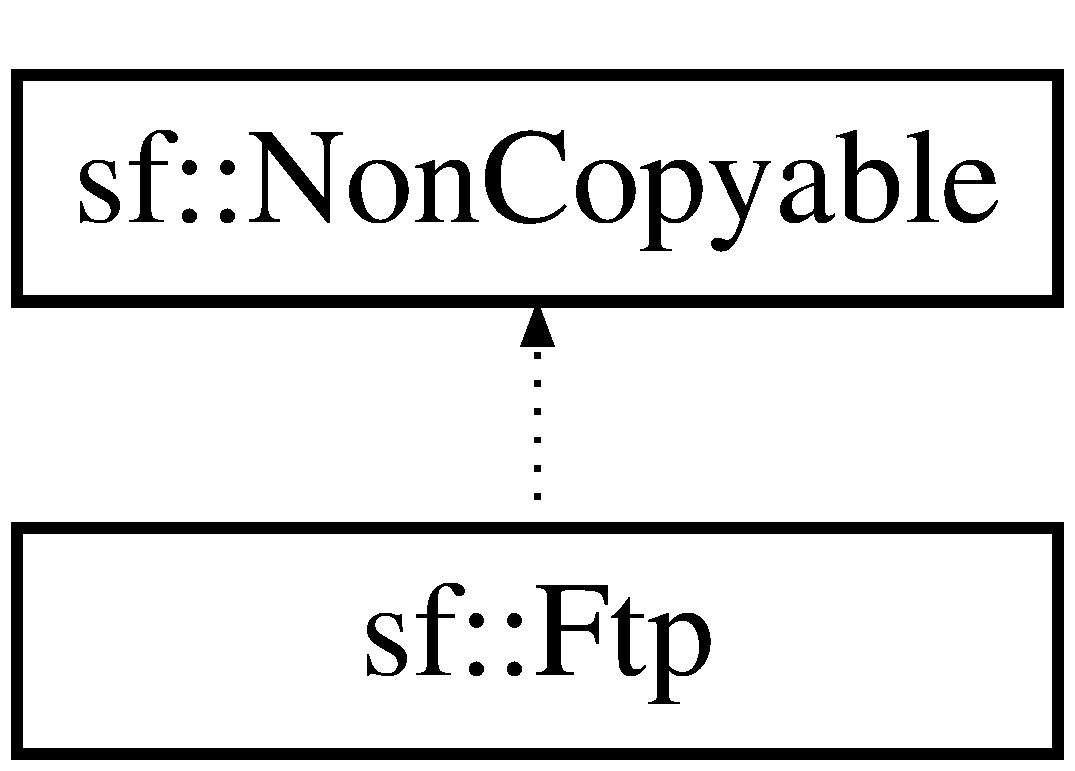
\includegraphics[height=2.000000cm]{classsf_1_1Ftp}
\end{center}
\end{figure}
\subsection*{Classes}
\begin{DoxyCompactItemize}
\item 
class \hyperlink{classsf_1_1Ftp_1_1DirectoryResponse}{Directory\-Response}
\begin{DoxyCompactList}\small\item\em Specialization of F\-T\-P response returning a directory. \end{DoxyCompactList}\item 
class \hyperlink{classsf_1_1Ftp_1_1ListingResponse}{Listing\-Response}
\begin{DoxyCompactList}\small\item\em Specialization of F\-T\-P response returning a filename lisiting. \end{DoxyCompactList}\item 
class \hyperlink{classsf_1_1Ftp_1_1Response}{Response}
\begin{DoxyCompactList}\small\item\em Define a F\-T\-P response. \end{DoxyCompactList}\end{DoxyCompactItemize}
\subsection*{Public Types}
\begin{DoxyCompactItemize}
\item 
enum \hyperlink{classsf_1_1Ftp_a1cd6b89ad23253f6d97e6d4ca4d558cb}{Transfer\-Mode} \{ \hyperlink{classsf_1_1Ftp_a1cd6b89ad23253f6d97e6d4ca4d558cba6f253b362639fb5e059dc292762a21ee}{Binary}, 
\hyperlink{classsf_1_1Ftp_a1cd6b89ad23253f6d97e6d4ca4d558cbac9e544a22dce8ef3177449cb235d15c2}{Ascii}, 
\hyperlink{classsf_1_1Ftp_a1cd6b89ad23253f6d97e6d4ca4d558cbabb1e34435231e73c96534c71090be7f4}{Ebcdic}
 \}
\begin{DoxyCompactList}\small\item\em Enumeration of transfer modes. \end{DoxyCompactList}\end{DoxyCompactItemize}
\subsection*{Public Member Functions}
\begin{DoxyCompactItemize}
\item 
\hyperlink{classsf_1_1Ftp_a2edfa8e9009caf27bce74459ae76dc52}{$\sim$\-Ftp} ()
\begin{DoxyCompactList}\small\item\em Destructor. \end{DoxyCompactList}\item 
\hyperlink{classsf_1_1Ftp_1_1Response}{Response} \hyperlink{classsf_1_1Ftp_af02fb3de3f450a50a27981961c69c860}{connect} (const \hyperlink{classsf_1_1IpAddress}{Ip\-Address} \&server, unsigned short port=21, \hyperlink{classsf_1_1Time}{Time} timeout=\hyperlink{classsf_1_1Time_a8db127b632fa8da21550e7282af11fa0}{Time\-::\-Zero})
\begin{DoxyCompactList}\small\item\em Connect to the specified F\-T\-P server. \end{DoxyCompactList}\item 
\hyperlink{classsf_1_1Ftp_1_1Response}{Response} \hyperlink{classsf_1_1Ftp_acf7459926f3391cd06bf84337ed6a0f4}{disconnect} ()
\begin{DoxyCompactList}\small\item\em Close the connection with the server. \end{DoxyCompactList}\item 
\hyperlink{classsf_1_1Ftp_1_1Response}{Response} \hyperlink{classsf_1_1Ftp_a686262bc377584cd50e52e1576aa3a9b}{login} ()
\begin{DoxyCompactList}\small\item\em Log in using an anonymous account. \end{DoxyCompactList}\item 
\hyperlink{classsf_1_1Ftp_1_1Response}{Response} \hyperlink{classsf_1_1Ftp_a99d8114793c1659e9d51d45cecdcd965}{login} (const std\-::string \&name, const std\-::string \&password)
\begin{DoxyCompactList}\small\item\em Log in using a username and a password. \end{DoxyCompactList}\item 
\hyperlink{classsf_1_1Ftp_1_1Response}{Response} \hyperlink{classsf_1_1Ftp_aa1127d442b4acb2105aa8060a39d04fc}{keep\-Alive} ()
\begin{DoxyCompactList}\small\item\em Send a null command to keep the connection alive. \end{DoxyCompactList}\item 
\hyperlink{classsf_1_1Ftp_1_1DirectoryResponse}{Directory\-Response} \hyperlink{classsf_1_1Ftp_a79c654fcdd0c81e68c4fa29af3b45e0c}{get\-Working\-Directory} ()
\begin{DoxyCompactList}\small\item\em Get the current working directory. \end{DoxyCompactList}\item 
\hyperlink{classsf_1_1Ftp_1_1ListingResponse}{Listing\-Response} \hyperlink{classsf_1_1Ftp_a8f37258e461fcb9e2a0655e9df0be4a0}{get\-Directory\-Listing} (const std\-::string \&directory=\char`\"{}\char`\"{})
\begin{DoxyCompactList}\small\item\em Get the contents of the given directory. \end{DoxyCompactList}\item 
\hyperlink{classsf_1_1Ftp_1_1Response}{Response} \hyperlink{classsf_1_1Ftp_a7e93488ea6330dd4dd76e428da9bb6d3}{change\-Directory} (const std\-::string \&directory)
\begin{DoxyCompactList}\small\item\em Change the current working directory. \end{DoxyCompactList}\item 
\hyperlink{classsf_1_1Ftp_1_1Response}{Response} \hyperlink{classsf_1_1Ftp_ad295cf77f30f9ad07b5c401fd9849189}{parent\-Directory} ()
\begin{DoxyCompactList}\small\item\em Go to the parent directory of the current one. \end{DoxyCompactList}\item 
\hyperlink{classsf_1_1Ftp_1_1Response}{Response} \hyperlink{classsf_1_1Ftp_a247b84c4b25da37804218c2b748c4787}{create\-Directory} (const std\-::string \&name)
\begin{DoxyCompactList}\small\item\em Create a new directory. \end{DoxyCompactList}\item 
\hyperlink{classsf_1_1Ftp_1_1Response}{Response} \hyperlink{classsf_1_1Ftp_a2a8a7ef9144204b5b319c9a4be8806c2}{delete\-Directory} (const std\-::string \&name)
\begin{DoxyCompactList}\small\item\em Remove an existing directory. \end{DoxyCompactList}\item 
\hyperlink{classsf_1_1Ftp_1_1Response}{Response} \hyperlink{classsf_1_1Ftp_a8f99251d7153e1dc26723e4006deb764}{rename\-File} (const std\-::string \&file, const std\-::string \&new\-Name)
\begin{DoxyCompactList}\small\item\em Rename an existing file. \end{DoxyCompactList}\item 
\hyperlink{classsf_1_1Ftp_1_1Response}{Response} \hyperlink{classsf_1_1Ftp_a8aa272b0eb7769a850006e70fcad370f}{delete\-File} (const std\-::string \&name)
\begin{DoxyCompactList}\small\item\em Remove an existing file. \end{DoxyCompactList}\item 
\hyperlink{classsf_1_1Ftp_1_1Response}{Response} \hyperlink{classsf_1_1Ftp_a20c1600ec5fd6f5a2ad1429ab8aa5df4}{download} (const std\-::string \&remote\-File, const std\-::string \&local\-Path, \hyperlink{classsf_1_1Ftp_a1cd6b89ad23253f6d97e6d4ca4d558cb}{Transfer\-Mode} mode=\hyperlink{classsf_1_1Ftp_a1cd6b89ad23253f6d97e6d4ca4d558cba6f253b362639fb5e059dc292762a21ee}{Binary})
\begin{DoxyCompactList}\small\item\em Download a file from the server. \end{DoxyCompactList}\item 
\hyperlink{classsf_1_1Ftp_1_1Response}{Response} \hyperlink{classsf_1_1Ftp_a46d6e15cddd719288b5a08b685e11765}{upload} (const std\-::string \&local\-File, const std\-::string \&remote\-Path, \hyperlink{classsf_1_1Ftp_a1cd6b89ad23253f6d97e6d4ca4d558cb}{Transfer\-Mode} mode=\hyperlink{classsf_1_1Ftp_a1cd6b89ad23253f6d97e6d4ca4d558cba6f253b362639fb5e059dc292762a21ee}{Binary})
\begin{DoxyCompactList}\small\item\em Upload a file to the server. \end{DoxyCompactList}\end{DoxyCompactItemize}
\subsection*{Friends}
\begin{DoxyCompactItemize}
\item 
\hypertarget{classsf_1_1Ftp_a8dee57337b6a7e183bfe21d178757b0c}{class {\bfseries Data\-Channel}}\label{classsf_1_1Ftp_a8dee57337b6a7e183bfe21d178757b0c}

\end{DoxyCompactItemize}


\subsection{Detailed Description}
A F\-T\-P client. 

\hyperlink{classsf_1_1Ftp}{sf\-::\-Ftp} is a very simple F\-T\-P client that allows you to communicate with a F\-T\-P server. The F\-T\-P protocol allows you to manipulate a remote file system (list files, upload, download, create, remove, ...).

Using the F\-T\-P client consists of 4 parts\-: \begin{DoxyItemize}
\item Connecting to the F\-T\-P server \item Logging in (either as a registered user or anonymously) \item Sending commands to the server \item Disconnecting (this part can be done implicitely by the destructor)\end{DoxyItemize}
Every command returns a F\-T\-P response, which contains the status code as well as a message from the server. Some commands such as get\-Working\-Directory and get\-Directory\-Listing return additional data, and use a class derived from \hyperlink{classsf_1_1Ftp_1_1Response}{sf\-::\-Ftp\-::\-Response} to provide this data.

All commands, especially upload and download, may take some time to complete. This is important to know if you don't want to block your application while the server is completing the task.

Usage example\-: 
\begin{DoxyCode}
\textcolor{comment}{// Create a new FTP client}
\hyperlink{classsf_1_1Ftp}{sf::Ftp} ftp;

\textcolor{comment}{// Connect to the server}
\hyperlink{classsf_1_1Ftp_1_1Response}{sf::Ftp::Response} response = ftp.\hyperlink{classsf_1_1Ftp_af02fb3de3f450a50a27981961c69c860}{connect}(\textcolor{stringliteral}{"ftp://ftp.myserver.com"});
\textcolor{keywordflow}{if} (response.\hyperlink{classsf_1_1Ftp_1_1Response_a4dadbe0fe0a3ef2d571a017e1645e675}{isOk}())
    std::cout << \textcolor{stringliteral}{"Connected"} << std::endl;

\textcolor{comment}{// Log in}
response = ftp.\hyperlink{classsf_1_1Ftp_a686262bc377584cd50e52e1576aa3a9b}{login}(\textcolor{stringliteral}{"laurent"}, \textcolor{stringliteral}{"dF6Zm89D"});
\textcolor{keywordflow}{if} (response.\hyperlink{classsf_1_1Ftp_1_1Response_a4dadbe0fe0a3ef2d571a017e1645e675}{isOk}())
    std::cout << \textcolor{stringliteral}{"Logged in"} << std::endl;

\textcolor{comment}{// Print the working directory}
\hyperlink{classsf_1_1Ftp_1_1DirectoryResponse}{sf::Ftp::DirectoryResponse} directory = ftp.
      \hyperlink{classsf_1_1Ftp_a79c654fcdd0c81e68c4fa29af3b45e0c}{getWorkingDirectory}();
\textcolor{keywordflow}{if} (directory.\hyperlink{classsf_1_1Ftp_1_1Response_a4dadbe0fe0a3ef2d571a017e1645e675}{isOk}())
    std::cout << \textcolor{stringliteral}{"Working directory: "} << directory.\hyperlink{classsf_1_1Ftp_1_1DirectoryResponse_a500793778ad0ed223aa86ed8fbee28a3}{getDirectory}() << std::endl;

\textcolor{comment}{// Create a new directory}
response = ftp.\hyperlink{classsf_1_1Ftp_a247b84c4b25da37804218c2b748c4787}{createDirectory}(\textcolor{stringliteral}{"files"});
\textcolor{keywordflow}{if} (response.\hyperlink{classsf_1_1Ftp_1_1Response_a4dadbe0fe0a3ef2d571a017e1645e675}{isOk}())
    std::cout << \textcolor{stringliteral}{"Created new directory"} << std::endl;

\textcolor{comment}{// Upload a file to this new directory}
response = ftp.\hyperlink{classsf_1_1Ftp_a46d6e15cddd719288b5a08b685e11765}{upload}(\textcolor{stringliteral}{"local-path/file.txt"}, \textcolor{stringliteral}{"files"}, \hyperlink{classsf_1_1Ftp_a1cd6b89ad23253f6d97e6d4ca4d558cbac9e544a22dce8ef3177449cb235d15c2}{sf::Ftp::Ascii});
\textcolor{keywordflow}{if} (response.\hyperlink{classsf_1_1Ftp_1_1Response_a4dadbe0fe0a3ef2d571a017e1645e675}{isOk}())
    std::cout << \textcolor{stringliteral}{"File uploaded"} << std::endl;

\textcolor{comment}{// Disconnect from the server (optional)}
ftp.\hyperlink{classsf_1_1Ftp_acf7459926f3391cd06bf84337ed6a0f4}{disconnect}();
\end{DoxyCode}
 

Definition at line 47 of file Ftp.\-hpp.



\subsection{Member Enumeration Documentation}
\hypertarget{classsf_1_1Ftp_a1cd6b89ad23253f6d97e6d4ca4d558cb}{\index{sf\-::\-Ftp@{sf\-::\-Ftp}!Transfer\-Mode@{Transfer\-Mode}}
\index{Transfer\-Mode@{Transfer\-Mode}!sf::Ftp@{sf\-::\-Ftp}}
\subsubsection[{Transfer\-Mode}]{\setlength{\rightskip}{0pt plus 5cm}enum {\bf sf\-::\-Ftp\-::\-Transfer\-Mode}}}\label{classsf_1_1Ftp_a1cd6b89ad23253f6d97e6d4ca4d558cb}


Enumeration of transfer modes. 

\begin{Desc}
\item[Enumerator]\par
\begin{description}
\index{Binary@{Binary}!sf\-::\-Ftp@{sf\-::\-Ftp}}\index{sf\-::\-Ftp@{sf\-::\-Ftp}!Binary@{Binary}}\item[{\em 
\hypertarget{classsf_1_1Ftp_a1cd6b89ad23253f6d97e6d4ca4d558cba6f253b362639fb5e059dc292762a21ee}{Binary}\label{classsf_1_1Ftp_a1cd6b89ad23253f6d97e6d4ca4d558cba6f253b362639fb5e059dc292762a21ee}
}]Binary mode (file is transfered as a sequence of bytes) \index{Ascii@{Ascii}!sf\-::\-Ftp@{sf\-::\-Ftp}}\index{sf\-::\-Ftp@{sf\-::\-Ftp}!Ascii@{Ascii}}\item[{\em 
\hypertarget{classsf_1_1Ftp_a1cd6b89ad23253f6d97e6d4ca4d558cbac9e544a22dce8ef3177449cb235d15c2}{Ascii}\label{classsf_1_1Ftp_a1cd6b89ad23253f6d97e6d4ca4d558cbac9e544a22dce8ef3177449cb235d15c2}
}]\hyperlink{classsf_1_1Text}{Text} mode using A\-S\-C\-I\-I encoding. \index{Ebcdic@{Ebcdic}!sf\-::\-Ftp@{sf\-::\-Ftp}}\index{sf\-::\-Ftp@{sf\-::\-Ftp}!Ebcdic@{Ebcdic}}\item[{\em 
\hypertarget{classsf_1_1Ftp_a1cd6b89ad23253f6d97e6d4ca4d558cbabb1e34435231e73c96534c71090be7f4}{Ebcdic}\label{classsf_1_1Ftp_a1cd6b89ad23253f6d97e6d4ca4d558cbabb1e34435231e73c96534c71090be7f4}
}]\hyperlink{classsf_1_1Text}{Text} mode using E\-B\-C\-D\-I\-C encoding. \end{description}
\end{Desc}


Definition at line 55 of file Ftp.\-hpp.



\subsection{Constructor \& Destructor Documentation}
\hypertarget{classsf_1_1Ftp_a2edfa8e9009caf27bce74459ae76dc52}{\index{sf\-::\-Ftp@{sf\-::\-Ftp}!$\sim$\-Ftp@{$\sim$\-Ftp}}
\index{$\sim$\-Ftp@{$\sim$\-Ftp}!sf::Ftp@{sf\-::\-Ftp}}
\subsubsection[{$\sim$\-Ftp}]{\setlength{\rightskip}{0pt plus 5cm}sf\-::\-Ftp\-::$\sim$\-Ftp (
\begin{DoxyParamCaption}
{}
\end{DoxyParamCaption}
)}}\label{classsf_1_1Ftp_a2edfa8e9009caf27bce74459ae76dc52}


Destructor. 

Automatically closes the connection with the server if it is still opened. 

\subsection{Member Function Documentation}
\hypertarget{classsf_1_1Ftp_a7e93488ea6330dd4dd76e428da9bb6d3}{\index{sf\-::\-Ftp@{sf\-::\-Ftp}!change\-Directory@{change\-Directory}}
\index{change\-Directory@{change\-Directory}!sf::Ftp@{sf\-::\-Ftp}}
\subsubsection[{change\-Directory}]{\setlength{\rightskip}{0pt plus 5cm}{\bf Response} sf\-::\-Ftp\-::change\-Directory (
\begin{DoxyParamCaption}
\item[{const std\-::string \&}]{directory}
\end{DoxyParamCaption}
)}}\label{classsf_1_1Ftp_a7e93488ea6330dd4dd76e428da9bb6d3}


Change the current working directory. 

The new directory must be relative to the current one.


\begin{DoxyParams}{Parameters}
{\em directory} & New working directory\\
\hline
\end{DoxyParams}
\begin{DoxyReturn}{Returns}
Server response to the request
\end{DoxyReturn}
\begin{DoxySeeAlso}{See Also}
\hyperlink{classsf_1_1Ftp_a79c654fcdd0c81e68c4fa29af3b45e0c}{get\-Working\-Directory}, \hyperlink{classsf_1_1Ftp_a8f37258e461fcb9e2a0655e9df0be4a0}{get\-Directory\-Listing}, \hyperlink{classsf_1_1Ftp_ad295cf77f30f9ad07b5c401fd9849189}{parent\-Directory} 
\end{DoxySeeAlso}
\hypertarget{classsf_1_1Ftp_af02fb3de3f450a50a27981961c69c860}{\index{sf\-::\-Ftp@{sf\-::\-Ftp}!connect@{connect}}
\index{connect@{connect}!sf::Ftp@{sf\-::\-Ftp}}
\subsubsection[{connect}]{\setlength{\rightskip}{0pt plus 5cm}{\bf Response} sf\-::\-Ftp\-::connect (
\begin{DoxyParamCaption}
\item[{const {\bf Ip\-Address} \&}]{server, }
\item[{unsigned short}]{port = {\ttfamily 21}, }
\item[{{\bf Time}}]{timeout = {\ttfamily {\bf Time\-::\-Zero}}}
\end{DoxyParamCaption}
)}}\label{classsf_1_1Ftp_af02fb3de3f450a50a27981961c69c860}


Connect to the specified F\-T\-P server. 

The port has a default value of 21, which is the standard port used by the F\-T\-P protocol. You shouldn't use a different value, unless you really know what you do. This function tries to connect to the server so it may take a while to complete, especially if the server is not reachable. To avoid blocking your application for too long, you can use a timeout. The default value, \hyperlink{classsf_1_1Time_a8db127b632fa8da21550e7282af11fa0}{Time\-::\-Zero}, means that the system timeout will be used (which is usually pretty long).


\begin{DoxyParams}{Parameters}
{\em server} & Name or address of the F\-T\-P server to connect to \\
\hline
{\em port} & Port used for the connection \\
\hline
{\em timeout} & Maximum time to wait\\
\hline
\end{DoxyParams}
\begin{DoxyReturn}{Returns}
Server response to the request
\end{DoxyReturn}
\begin{DoxySeeAlso}{See Also}
\hyperlink{classsf_1_1Ftp_acf7459926f3391cd06bf84337ed6a0f4}{disconnect} 
\end{DoxySeeAlso}
\hypertarget{classsf_1_1Ftp_a247b84c4b25da37804218c2b748c4787}{\index{sf\-::\-Ftp@{sf\-::\-Ftp}!create\-Directory@{create\-Directory}}
\index{create\-Directory@{create\-Directory}!sf::Ftp@{sf\-::\-Ftp}}
\subsubsection[{create\-Directory}]{\setlength{\rightskip}{0pt plus 5cm}{\bf Response} sf\-::\-Ftp\-::create\-Directory (
\begin{DoxyParamCaption}
\item[{const std\-::string \&}]{name}
\end{DoxyParamCaption}
)}}\label{classsf_1_1Ftp_a247b84c4b25da37804218c2b748c4787}


Create a new directory. 

The new directory is created as a child of the current working directory.


\begin{DoxyParams}{Parameters}
{\em name} & Name of the directory to create\\
\hline
\end{DoxyParams}
\begin{DoxyReturn}{Returns}
Server response to the request
\end{DoxyReturn}
\begin{DoxySeeAlso}{See Also}
\hyperlink{classsf_1_1Ftp_a2a8a7ef9144204b5b319c9a4be8806c2}{delete\-Directory} 
\end{DoxySeeAlso}
\hypertarget{classsf_1_1Ftp_a2a8a7ef9144204b5b319c9a4be8806c2}{\index{sf\-::\-Ftp@{sf\-::\-Ftp}!delete\-Directory@{delete\-Directory}}
\index{delete\-Directory@{delete\-Directory}!sf::Ftp@{sf\-::\-Ftp}}
\subsubsection[{delete\-Directory}]{\setlength{\rightskip}{0pt plus 5cm}{\bf Response} sf\-::\-Ftp\-::delete\-Directory (
\begin{DoxyParamCaption}
\item[{const std\-::string \&}]{name}
\end{DoxyParamCaption}
)}}\label{classsf_1_1Ftp_a2a8a7ef9144204b5b319c9a4be8806c2}


Remove an existing directory. 

The directory to remove must be relative to the current working directory. Use this function with caution, the directory will be removed permanently!


\begin{DoxyParams}{Parameters}
{\em name} & Name of the directory to remove\\
\hline
\end{DoxyParams}
\begin{DoxyReturn}{Returns}
Server response to the request
\end{DoxyReturn}
\begin{DoxySeeAlso}{See Also}
\hyperlink{classsf_1_1Ftp_a247b84c4b25da37804218c2b748c4787}{create\-Directory} 
\end{DoxySeeAlso}
\hypertarget{classsf_1_1Ftp_a8aa272b0eb7769a850006e70fcad370f}{\index{sf\-::\-Ftp@{sf\-::\-Ftp}!delete\-File@{delete\-File}}
\index{delete\-File@{delete\-File}!sf::Ftp@{sf\-::\-Ftp}}
\subsubsection[{delete\-File}]{\setlength{\rightskip}{0pt plus 5cm}{\bf Response} sf\-::\-Ftp\-::delete\-File (
\begin{DoxyParamCaption}
\item[{const std\-::string \&}]{name}
\end{DoxyParamCaption}
)}}\label{classsf_1_1Ftp_a8aa272b0eb7769a850006e70fcad370f}


Remove an existing file. 

The file name must be relative to the current working directory. Use this function with caution, the file will be removed permanently!


\begin{DoxyParams}{Parameters}
{\em name} & File to remove\\
\hline
\end{DoxyParams}
\begin{DoxyReturn}{Returns}
Server response to the request
\end{DoxyReturn}
\begin{DoxySeeAlso}{See Also}
\hyperlink{classsf_1_1Ftp_a8f99251d7153e1dc26723e4006deb764}{rename\-File} 
\end{DoxySeeAlso}
\hypertarget{classsf_1_1Ftp_acf7459926f3391cd06bf84337ed6a0f4}{\index{sf\-::\-Ftp@{sf\-::\-Ftp}!disconnect@{disconnect}}
\index{disconnect@{disconnect}!sf::Ftp@{sf\-::\-Ftp}}
\subsubsection[{disconnect}]{\setlength{\rightskip}{0pt plus 5cm}{\bf Response} sf\-::\-Ftp\-::disconnect (
\begin{DoxyParamCaption}
{}
\end{DoxyParamCaption}
)}}\label{classsf_1_1Ftp_acf7459926f3391cd06bf84337ed6a0f4}


Close the connection with the server. 

\begin{DoxyReturn}{Returns}
Server response to the request
\end{DoxyReturn}
\begin{DoxySeeAlso}{See Also}
\hyperlink{classsf_1_1Ftp_af02fb3de3f450a50a27981961c69c860}{connect} 
\end{DoxySeeAlso}
\hypertarget{classsf_1_1Ftp_a20c1600ec5fd6f5a2ad1429ab8aa5df4}{\index{sf\-::\-Ftp@{sf\-::\-Ftp}!download@{download}}
\index{download@{download}!sf::Ftp@{sf\-::\-Ftp}}
\subsubsection[{download}]{\setlength{\rightskip}{0pt plus 5cm}{\bf Response} sf\-::\-Ftp\-::download (
\begin{DoxyParamCaption}
\item[{const std\-::string \&}]{remote\-File, }
\item[{const std\-::string \&}]{local\-Path, }
\item[{{\bf Transfer\-Mode}}]{mode = {\ttfamily {\bf Binary}}}
\end{DoxyParamCaption}
)}}\label{classsf_1_1Ftp_a20c1600ec5fd6f5a2ad1429ab8aa5df4}


Download a file from the server. 

The filename of the distant file is relative to the current working directory of the server, and the local destination path is relative to the current directory of your application.


\begin{DoxyParams}{Parameters}
{\em remote\-File} & Filename of the distant file to download \\
\hline
{\em local\-Path} & Where to put to file on the local computer \\
\hline
{\em mode} & Transfer mode\\
\hline
\end{DoxyParams}
\begin{DoxyReturn}{Returns}
Server response to the request
\end{DoxyReturn}
\begin{DoxySeeAlso}{See Also}
\hyperlink{classsf_1_1Ftp_a46d6e15cddd719288b5a08b685e11765}{upload} 
\end{DoxySeeAlso}
\hypertarget{classsf_1_1Ftp_a8f37258e461fcb9e2a0655e9df0be4a0}{\index{sf\-::\-Ftp@{sf\-::\-Ftp}!get\-Directory\-Listing@{get\-Directory\-Listing}}
\index{get\-Directory\-Listing@{get\-Directory\-Listing}!sf::Ftp@{sf\-::\-Ftp}}
\subsubsection[{get\-Directory\-Listing}]{\setlength{\rightskip}{0pt plus 5cm}{\bf Listing\-Response} sf\-::\-Ftp\-::get\-Directory\-Listing (
\begin{DoxyParamCaption}
\item[{const std\-::string \&}]{directory = {\ttfamily \char`\"{}\char`\"{}}}
\end{DoxyParamCaption}
)}}\label{classsf_1_1Ftp_a8f37258e461fcb9e2a0655e9df0be4a0}


Get the contents of the given directory. 

This function retrieves the sub-\/directories and files contained in the given directory. It is not recursive. The {\itshape directory} parameter is relative to the current working directory.


\begin{DoxyParams}{Parameters}
{\em directory} & Directory to list\\
\hline
\end{DoxyParams}
\begin{DoxyReturn}{Returns}
Server response to the request
\end{DoxyReturn}
\begin{DoxySeeAlso}{See Also}
\hyperlink{classsf_1_1Ftp_a79c654fcdd0c81e68c4fa29af3b45e0c}{get\-Working\-Directory}, \hyperlink{classsf_1_1Ftp_a7e93488ea6330dd4dd76e428da9bb6d3}{change\-Directory}, \hyperlink{classsf_1_1Ftp_ad295cf77f30f9ad07b5c401fd9849189}{parent\-Directory} 
\end{DoxySeeAlso}
\hypertarget{classsf_1_1Ftp_a79c654fcdd0c81e68c4fa29af3b45e0c}{\index{sf\-::\-Ftp@{sf\-::\-Ftp}!get\-Working\-Directory@{get\-Working\-Directory}}
\index{get\-Working\-Directory@{get\-Working\-Directory}!sf::Ftp@{sf\-::\-Ftp}}
\subsubsection[{get\-Working\-Directory}]{\setlength{\rightskip}{0pt plus 5cm}{\bf Directory\-Response} sf\-::\-Ftp\-::get\-Working\-Directory (
\begin{DoxyParamCaption}
{}
\end{DoxyParamCaption}
)}}\label{classsf_1_1Ftp_a79c654fcdd0c81e68c4fa29af3b45e0c}


Get the current working directory. 

The working directory is the root path for subsequent operations involving directories and/or filenames.

\begin{DoxyReturn}{Returns}
Server response to the request
\end{DoxyReturn}
\begin{DoxySeeAlso}{See Also}
\hyperlink{classsf_1_1Ftp_a8f37258e461fcb9e2a0655e9df0be4a0}{get\-Directory\-Listing}, \hyperlink{classsf_1_1Ftp_a7e93488ea6330dd4dd76e428da9bb6d3}{change\-Directory}, \hyperlink{classsf_1_1Ftp_ad295cf77f30f9ad07b5c401fd9849189}{parent\-Directory} 
\end{DoxySeeAlso}
\hypertarget{classsf_1_1Ftp_aa1127d442b4acb2105aa8060a39d04fc}{\index{sf\-::\-Ftp@{sf\-::\-Ftp}!keep\-Alive@{keep\-Alive}}
\index{keep\-Alive@{keep\-Alive}!sf::Ftp@{sf\-::\-Ftp}}
\subsubsection[{keep\-Alive}]{\setlength{\rightskip}{0pt plus 5cm}{\bf Response} sf\-::\-Ftp\-::keep\-Alive (
\begin{DoxyParamCaption}
{}
\end{DoxyParamCaption}
)}}\label{classsf_1_1Ftp_aa1127d442b4acb2105aa8060a39d04fc}


Send a null command to keep the connection alive. 

This command is useful because the server may close the connection automatically if no command is sent.

\begin{DoxyReturn}{Returns}
Server response to the request 
\end{DoxyReturn}
\hypertarget{classsf_1_1Ftp_a686262bc377584cd50e52e1576aa3a9b}{\index{sf\-::\-Ftp@{sf\-::\-Ftp}!login@{login}}
\index{login@{login}!sf::Ftp@{sf\-::\-Ftp}}
\subsubsection[{login}]{\setlength{\rightskip}{0pt plus 5cm}{\bf Response} sf\-::\-Ftp\-::login (
\begin{DoxyParamCaption}
{}
\end{DoxyParamCaption}
)}}\label{classsf_1_1Ftp_a686262bc377584cd50e52e1576aa3a9b}


Log in using an anonymous account. 

Logging in is mandatory after connecting to the server. Users that are not logged in cannot perform any operation.

\begin{DoxyReturn}{Returns}
Server response to the request 
\end{DoxyReturn}
\hypertarget{classsf_1_1Ftp_a99d8114793c1659e9d51d45cecdcd965}{\index{sf\-::\-Ftp@{sf\-::\-Ftp}!login@{login}}
\index{login@{login}!sf::Ftp@{sf\-::\-Ftp}}
\subsubsection[{login}]{\setlength{\rightskip}{0pt plus 5cm}{\bf Response} sf\-::\-Ftp\-::login (
\begin{DoxyParamCaption}
\item[{const std\-::string \&}]{name, }
\item[{const std\-::string \&}]{password}
\end{DoxyParamCaption}
)}}\label{classsf_1_1Ftp_a99d8114793c1659e9d51d45cecdcd965}


Log in using a username and a password. 

Logging in is mandatory after connecting to the server. Users that are not logged in cannot perform any operation.


\begin{DoxyParams}{Parameters}
{\em name} & User name \\
\hline
{\em password} & Password\\
\hline
\end{DoxyParams}
\begin{DoxyReturn}{Returns}
Server response to the request 
\end{DoxyReturn}
\hypertarget{classsf_1_1Ftp_ad295cf77f30f9ad07b5c401fd9849189}{\index{sf\-::\-Ftp@{sf\-::\-Ftp}!parent\-Directory@{parent\-Directory}}
\index{parent\-Directory@{parent\-Directory}!sf::Ftp@{sf\-::\-Ftp}}
\subsubsection[{parent\-Directory}]{\setlength{\rightskip}{0pt plus 5cm}{\bf Response} sf\-::\-Ftp\-::parent\-Directory (
\begin{DoxyParamCaption}
{}
\end{DoxyParamCaption}
)}}\label{classsf_1_1Ftp_ad295cf77f30f9ad07b5c401fd9849189}


Go to the parent directory of the current one. 

\begin{DoxyReturn}{Returns}
Server response to the request
\end{DoxyReturn}
\begin{DoxySeeAlso}{See Also}
\hyperlink{classsf_1_1Ftp_a79c654fcdd0c81e68c4fa29af3b45e0c}{get\-Working\-Directory}, \hyperlink{classsf_1_1Ftp_a8f37258e461fcb9e2a0655e9df0be4a0}{get\-Directory\-Listing}, \hyperlink{classsf_1_1Ftp_a7e93488ea6330dd4dd76e428da9bb6d3}{change\-Directory} 
\end{DoxySeeAlso}
\hypertarget{classsf_1_1Ftp_a8f99251d7153e1dc26723e4006deb764}{\index{sf\-::\-Ftp@{sf\-::\-Ftp}!rename\-File@{rename\-File}}
\index{rename\-File@{rename\-File}!sf::Ftp@{sf\-::\-Ftp}}
\subsubsection[{rename\-File}]{\setlength{\rightskip}{0pt plus 5cm}{\bf Response} sf\-::\-Ftp\-::rename\-File (
\begin{DoxyParamCaption}
\item[{const std\-::string \&}]{file, }
\item[{const std\-::string \&}]{new\-Name}
\end{DoxyParamCaption}
)}}\label{classsf_1_1Ftp_a8f99251d7153e1dc26723e4006deb764}


Rename an existing file. 

The filenames must be relative to the current working directory.


\begin{DoxyParams}{Parameters}
{\em file} & File to rename \\
\hline
{\em new\-Name} & New name of the file\\
\hline
\end{DoxyParams}
\begin{DoxyReturn}{Returns}
Server response to the request
\end{DoxyReturn}
\begin{DoxySeeAlso}{See Also}
\hyperlink{classsf_1_1Ftp_a8aa272b0eb7769a850006e70fcad370f}{delete\-File} 
\end{DoxySeeAlso}
\hypertarget{classsf_1_1Ftp_a46d6e15cddd719288b5a08b685e11765}{\index{sf\-::\-Ftp@{sf\-::\-Ftp}!upload@{upload}}
\index{upload@{upload}!sf::Ftp@{sf\-::\-Ftp}}
\subsubsection[{upload}]{\setlength{\rightskip}{0pt plus 5cm}{\bf Response} sf\-::\-Ftp\-::upload (
\begin{DoxyParamCaption}
\item[{const std\-::string \&}]{local\-File, }
\item[{const std\-::string \&}]{remote\-Path, }
\item[{{\bf Transfer\-Mode}}]{mode = {\ttfamily {\bf Binary}}}
\end{DoxyParamCaption}
)}}\label{classsf_1_1Ftp_a46d6e15cddd719288b5a08b685e11765}


Upload a file to the server. 

The name of the local file is relative to the current working directory of your application, and the remote path is relative to the current directory of the F\-T\-P server.


\begin{DoxyParams}{Parameters}
{\em local\-File} & Path of the local file to upload \\
\hline
{\em remote\-Path} & Where to put to file on the server \\
\hline
{\em mode} & Transfer mode\\
\hline
\end{DoxyParams}
\begin{DoxyReturn}{Returns}
Server response to the request
\end{DoxyReturn}
\begin{DoxySeeAlso}{See Also}
\hyperlink{classsf_1_1Ftp_a20c1600ec5fd6f5a2ad1429ab8aa5df4}{download} 
\end{DoxySeeAlso}


The documentation for this class was generated from the following file\-:\begin{DoxyCompactItemize}
\item 
/home/z\-Zelman/\-Dropbox/\-Placeholder-\/\-R\-T\-S/\-S\-F\-M\-L-\/2.\-1/include/\-S\-F\-M\-L/\-Network/Ftp.\-hpp\end{DoxyCompactItemize}

\hypertarget{classsf_1_1GlResource}{\section{sf\-:\-:Gl\-Resource Class Reference}
\label{classsf_1_1GlResource}\index{sf\-::\-Gl\-Resource@{sf\-::\-Gl\-Resource}}
}


Base class for classes that require an Open\-G\-L context.  




{\ttfamily \#include $<$Gl\-Resource.\-hpp$>$}

Inheritance diagram for sf\-:\-:Gl\-Resource\-:\begin{figure}[H]
\begin{center}
\leavevmode
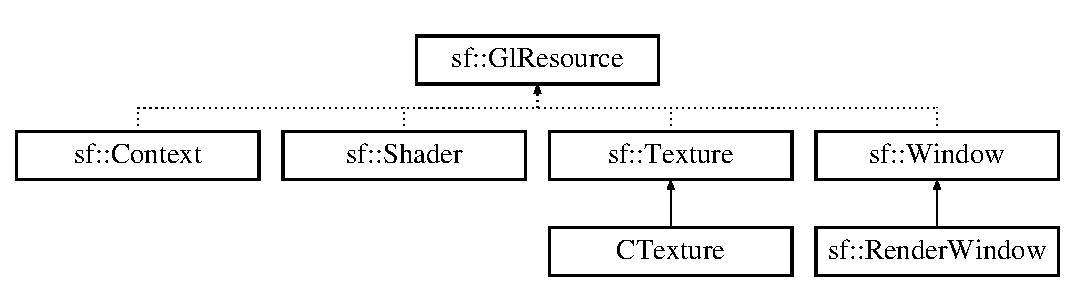
\includegraphics[height=3.000000cm]{classsf_1_1GlResource}
\end{center}
\end{figure}
\subsection*{Protected Member Functions}
\begin{DoxyCompactItemize}
\item 
\hypertarget{classsf_1_1GlResource_ad8fb7a0674f0f77e530dacc2a3b0dc6a}{\hyperlink{classsf_1_1GlResource_ad8fb7a0674f0f77e530dacc2a3b0dc6a}{Gl\-Resource} ()}\label{classsf_1_1GlResource_ad8fb7a0674f0f77e530dacc2a3b0dc6a}

\begin{DoxyCompactList}\small\item\em Default constructor. \end{DoxyCompactList}\item 
\hypertarget{classsf_1_1GlResource_ab99035b67052331d1e8cf67abd93de98}{\hyperlink{classsf_1_1GlResource_ab99035b67052331d1e8cf67abd93de98}{$\sim$\-Gl\-Resource} ()}\label{classsf_1_1GlResource_ab99035b67052331d1e8cf67abd93de98}

\begin{DoxyCompactList}\small\item\em Destructor. \end{DoxyCompactList}\end{DoxyCompactItemize}
\subsection*{Static Protected Member Functions}
\begin{DoxyCompactItemize}
\item 
\hypertarget{classsf_1_1GlResource_ae0efa7935241644608ca32ba47b22a33}{static void \hyperlink{classsf_1_1GlResource_ae0efa7935241644608ca32ba47b22a33}{ensure\-Gl\-Context} ()}\label{classsf_1_1GlResource_ae0efa7935241644608ca32ba47b22a33}

\begin{DoxyCompactList}\small\item\em Make sure that a valid Open\-G\-L context exists in the current thread. \end{DoxyCompactList}\end{DoxyCompactItemize}


\subsection{Detailed Description}
Base class for classes that require an Open\-G\-L context. 

This class is for internal use only, it must be the base of every class that requires a valid Open\-G\-L context in order to work. 

Definition at line 40 of file Gl\-Resource.\-hpp.



The documentation for this class was generated from the following file\-:\begin{DoxyCompactItemize}
\item 
/home/z\-Zelman/\-Dropbox/\-Placeholder-\/\-R\-T\-S/\-S\-F\-M\-L-\/2.\-1/include/\-S\-F\-M\-L/\-Window/Gl\-Resource.\-hpp\end{DoxyCompactItemize}

\hypertarget{classsf_1_1Glyph}{\section{sf\-:\-:Glyph Class Reference}
\label{classsf_1_1Glyph}\index{sf\-::\-Glyph@{sf\-::\-Glyph}}
}


Structure describing a glyph.  




{\ttfamily \#include $<$Glyph.\-hpp$>$}

\subsection*{Public Member Functions}
\begin{DoxyCompactItemize}
\item 
\hypertarget{classsf_1_1Glyph_ab15cfc37eb7b40a94b3b3aedf934010b}{\hyperlink{classsf_1_1Glyph_ab15cfc37eb7b40a94b3b3aedf934010b}{Glyph} ()}\label{classsf_1_1Glyph_ab15cfc37eb7b40a94b3b3aedf934010b}

\begin{DoxyCompactList}\small\item\em Default constructor. \end{DoxyCompactList}\end{DoxyCompactItemize}
\subsection*{Public Attributes}
\begin{DoxyCompactItemize}
\item 
\hypertarget{classsf_1_1Glyph_a50b93f441db501d10308007f63382166}{int \hyperlink{classsf_1_1Glyph_a50b93f441db501d10308007f63382166}{advance}}\label{classsf_1_1Glyph_a50b93f441db501d10308007f63382166}

\begin{DoxyCompactList}\small\item\em Offset to move horizontically to the next character. \end{DoxyCompactList}\item 
\hypertarget{classsf_1_1Glyph_afe4cd37e5839955d7dd008e178d41f0c}{\hyperlink{classsf_1_1Rect}{Int\-Rect} \hyperlink{classsf_1_1Glyph_afe4cd37e5839955d7dd008e178d41f0c}{bounds}}\label{classsf_1_1Glyph_afe4cd37e5839955d7dd008e178d41f0c}

\begin{DoxyCompactList}\small\item\em Bounding rectangle of the glyph, in coordinates relative to the baseline. \end{DoxyCompactList}\item 
\hypertarget{classsf_1_1Glyph_a0d502d326449f8c49011ed91d2805f5b}{\hyperlink{classsf_1_1Rect}{Int\-Rect} \hyperlink{classsf_1_1Glyph_a0d502d326449f8c49011ed91d2805f5b}{texture\-Rect}}\label{classsf_1_1Glyph_a0d502d326449f8c49011ed91d2805f5b}

\begin{DoxyCompactList}\small\item\em \hyperlink{classsf_1_1Texture}{Texture} coordinates of the glyph inside the font's texture. \end{DoxyCompactList}\end{DoxyCompactItemize}


\subsection{Detailed Description}
Structure describing a glyph. 

A glyph is the visual representation of a character.

The \hyperlink{classsf_1_1Glyph}{sf\-::\-Glyph} structure provides the information needed to handle the glyph\-: \begin{DoxyItemize}
\item its coordinates in the font's texture \item its bounding rectangle \item the offset to apply to get the starting position of the next glyph\end{DoxyItemize}
\begin{DoxySeeAlso}{See Also}
\hyperlink{classsf_1_1Font}{sf\-::\-Font} 
\end{DoxySeeAlso}


Definition at line 41 of file Glyph.\-hpp.



The documentation for this class was generated from the following file\-:\begin{DoxyCompactItemize}
\item 
/home/z\-Zelman/\-Dropbox/\-Placeholder-\/\-R\-T\-S/\-S\-F\-M\-L-\/2.\-1/include/\-S\-F\-M\-L/\-Graphics/Glyph.\-hpp\end{DoxyCompactItemize}

\hypertarget{classsf_1_1Http}{\section{sf\-:\-:Http Class Reference}
\label{classsf_1_1Http}\index{sf\-::\-Http@{sf\-::\-Http}}
}


A H\-T\-T\-P client.  




{\ttfamily \#include $<$Http.\-hpp$>$}

Inheritance diagram for sf\-:\-:Http\-:\begin{figure}[H]
\begin{center}
\leavevmode
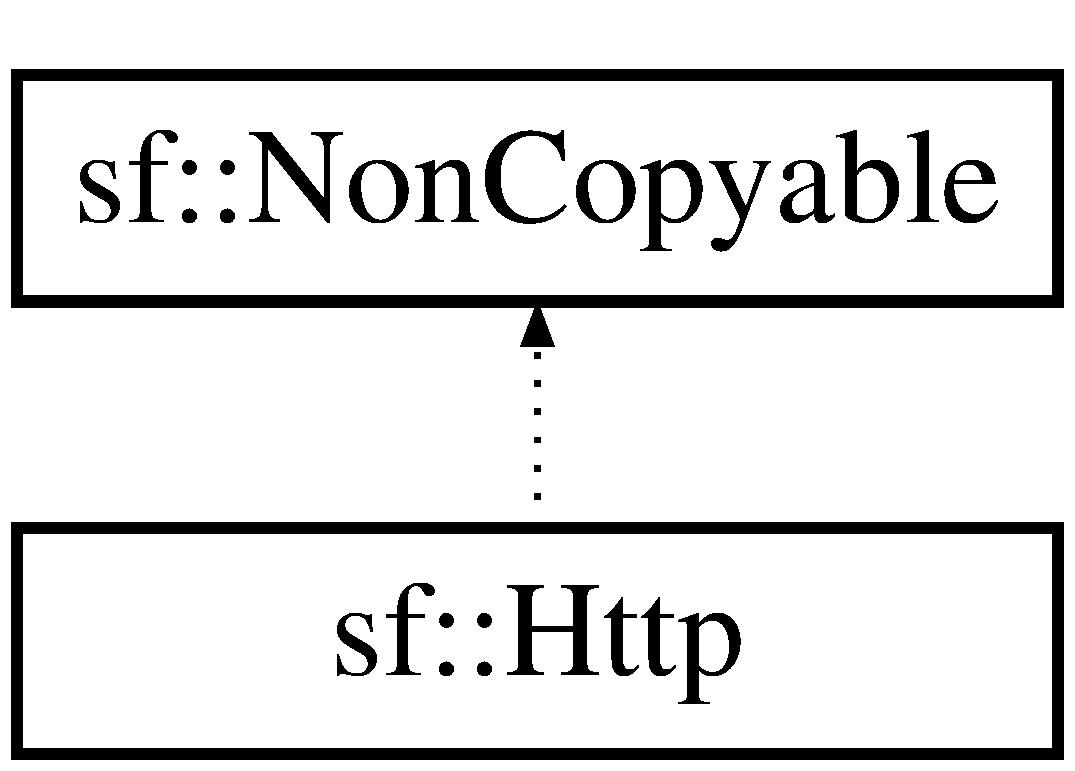
\includegraphics[height=2.000000cm]{classsf_1_1Http}
\end{center}
\end{figure}
\subsection*{Classes}
\begin{DoxyCompactItemize}
\item 
class \hyperlink{classsf_1_1Http_1_1Request}{Request}
\begin{DoxyCompactList}\small\item\em Define a H\-T\-T\-P request. \end{DoxyCompactList}\item 
class \hyperlink{classsf_1_1Http_1_1Response}{Response}
\begin{DoxyCompactList}\small\item\em Define a H\-T\-T\-P response. \end{DoxyCompactList}\end{DoxyCompactItemize}
\subsection*{Public Member Functions}
\begin{DoxyCompactItemize}
\item 
\hypertarget{classsf_1_1Http_abe2360194f99bdde402c9f97a85cf067}{\hyperlink{classsf_1_1Http_abe2360194f99bdde402c9f97a85cf067}{Http} ()}\label{classsf_1_1Http_abe2360194f99bdde402c9f97a85cf067}

\begin{DoxyCompactList}\small\item\em Default constructor. \end{DoxyCompactList}\item 
\hyperlink{classsf_1_1Http_a79efd844a735f083fcce0edbf1092385}{Http} (const std\-::string \&host, unsigned short port=0)
\begin{DoxyCompactList}\small\item\em Construct the H\-T\-T\-P client with the target host. \end{DoxyCompactList}\item 
void \hyperlink{classsf_1_1Http_a55121d543b61c41cf20b885a97b04e65}{set\-Host} (const std\-::string \&host, unsigned short port=0)
\begin{DoxyCompactList}\small\item\em Set the target host. \end{DoxyCompactList}\item 
\hyperlink{classsf_1_1Http_1_1Response}{Response} \hyperlink{classsf_1_1Http_aaf09ebfb5e00dcc82e0d494d5c6a9e2a}{send\-Request} (const \hyperlink{classsf_1_1Http_1_1Request}{Request} \&request, \hyperlink{classsf_1_1Time}{Time} timeout=\hyperlink{classsf_1_1Time_a8db127b632fa8da21550e7282af11fa0}{Time\-::\-Zero})
\begin{DoxyCompactList}\small\item\em Send a H\-T\-T\-P request and return the server's response. \end{DoxyCompactList}\end{DoxyCompactItemize}


\subsection{Detailed Description}
A H\-T\-T\-P client. 

\hyperlink{classsf_1_1Http}{sf\-::\-Http} is a very simple H\-T\-T\-P client that allows you to communicate with a web server. You can retrieve web pages, send data to an interactive resource, download a remote file, etc.

The H\-T\-T\-P client is split into 3 classes\-: \begin{DoxyItemize}
\item \hyperlink{classsf_1_1Http_1_1Request}{sf\-::\-Http\-::\-Request} \item \hyperlink{classsf_1_1Http_1_1Response}{sf\-::\-Http\-::\-Response} \item \hyperlink{classsf_1_1Http}{sf\-::\-Http}\end{DoxyItemize}
\hyperlink{classsf_1_1Http_1_1Request}{sf\-::\-Http\-::\-Request} builds the request that will be sent to the server. A request is made of\-: \begin{DoxyItemize}
\item a method (what you want to do) \item a target U\-R\-I (usually the name of the web page or file) \item one or more header fields (options that you can pass to the server) \item an optional body (for P\-O\-S\-T requests)\end{DoxyItemize}
\hyperlink{classsf_1_1Http_1_1Response}{sf\-::\-Http\-::\-Response} parse the response from the web server and provides getters to read them. The response contains\-: \begin{DoxyItemize}
\item a status code \item header fields (that may be answers to the ones that you requested) \item a body, which contains the contents of the requested resource\end{DoxyItemize}
\hyperlink{classsf_1_1Http}{sf\-::\-Http} provides a simple function, Send\-Request, to send a \hyperlink{classsf_1_1Http_1_1Request}{sf\-::\-Http\-::\-Request} and return the corresponding \hyperlink{classsf_1_1Http_1_1Response}{sf\-::\-Http\-::\-Response} from the server.

Usage example\-: 
\begin{DoxyCode}
\textcolor{comment}{// Create a new HTTP client}
\hyperlink{classsf_1_1Http}{sf::Http} http;

\textcolor{comment}{// We'll work on http://www.sfml-dev.org}
http.\hyperlink{classsf_1_1Http_a55121d543b61c41cf20b885a97b04e65}{setHost}(\textcolor{stringliteral}{"http://www.sfml-dev.org"});

\textcolor{comment}{// Prepare a request to get the 'features.php' page}
\hyperlink{classsf_1_1Http_1_1Request}{sf::Http::Request} request(\textcolor{stringliteral}{"features.php"});

\textcolor{comment}{// Send the request}
\hyperlink{classsf_1_1Http_1_1Response}{sf::Http::Response} response = http.\hyperlink{classsf_1_1Http_aaf09ebfb5e00dcc82e0d494d5c6a9e2a}{sendRequest}(request);

\textcolor{comment}{// Check the status code and display the result}
\hyperlink{classsf_1_1Http_1_1Response_a663e071978e30fbbeb20ed045be874d8}{sf::Http::Response::Status} status = response.\hyperlink{classsf_1_1Http_1_1Response_a542e9856b1dd260a83940eb982b7f19a}{getStatus}();
\textcolor{keywordflow}{if} (status == \hyperlink{classsf_1_1Http_1_1Response_a663e071978e30fbbeb20ed045be874d8a0158f932254d3f09647dd1f64bd43832}{sf::Http::Response::Ok})
\{
    std::cout << response.\hyperlink{classsf_1_1Http_1_1Response_a6b74ef73051a16ebb20041495c758e22}{getBody}() << std::endl;
\}
\textcolor{keywordflow}{else}
\{
    std::cout << \textcolor{stringliteral}{"Error "} << status << std::endl;
\}
\end{DoxyCode}
 

Definition at line 46 of file Http.\-hpp.



\subsection{Constructor \& Destructor Documentation}
\hypertarget{classsf_1_1Http_a79efd844a735f083fcce0edbf1092385}{\index{sf\-::\-Http@{sf\-::\-Http}!Http@{Http}}
\index{Http@{Http}!sf::Http@{sf\-::\-Http}}
\subsubsection[{Http}]{\setlength{\rightskip}{0pt plus 5cm}sf\-::\-Http\-::\-Http (
\begin{DoxyParamCaption}
\item[{const std\-::string \&}]{host, }
\item[{unsigned short}]{port = {\ttfamily 0}}
\end{DoxyParamCaption}
)}}\label{classsf_1_1Http_a79efd844a735f083fcce0edbf1092385}


Construct the H\-T\-T\-P client with the target host. 

This is equivalent to calling set\-Host(host, port). The port has a default value of 0, which means that the H\-T\-T\-P client will use the right port according to the protocol used (80 for H\-T\-T\-P, 443 for H\-T\-T\-P\-S). You should leave it like this unless you really need a port other than the standard one, or use an unknown protocol.


\begin{DoxyParams}{Parameters}
{\em host} & Web server to connect to \\
\hline
{\em port} & Port to use for connection \\
\hline
\end{DoxyParams}


\subsection{Member Function Documentation}
\hypertarget{classsf_1_1Http_aaf09ebfb5e00dcc82e0d494d5c6a9e2a}{\index{sf\-::\-Http@{sf\-::\-Http}!send\-Request@{send\-Request}}
\index{send\-Request@{send\-Request}!sf::Http@{sf\-::\-Http}}
\subsubsection[{send\-Request}]{\setlength{\rightskip}{0pt plus 5cm}{\bf Response} sf\-::\-Http\-::send\-Request (
\begin{DoxyParamCaption}
\item[{const {\bf Request} \&}]{request, }
\item[{{\bf Time}}]{timeout = {\ttfamily {\bf Time\-::\-Zero}}}
\end{DoxyParamCaption}
)}}\label{classsf_1_1Http_aaf09ebfb5e00dcc82e0d494d5c6a9e2a}


Send a H\-T\-T\-P request and return the server's response. 

You must have a valid host before sending a request (see set\-Host). Any missing mandatory header field in the request will be added with an appropriate value. Warning\-: this function waits for the server's response and may not return instantly; use a thread if you don't want to block your application, or use a timeout to limit the time to wait. A value of \hyperlink{classsf_1_1Time_a8db127b632fa8da21550e7282af11fa0}{Time\-::\-Zero} means that the client will use the system defaut timeout (which is usually pretty long).


\begin{DoxyParams}{Parameters}
{\em request} & \hyperlink{classsf_1_1Http_1_1Request}{Request} to send \\
\hline
{\em timeout} & Maximum time to wait\\
\hline
\end{DoxyParams}
\begin{DoxyReturn}{Returns}
Server's response 
\end{DoxyReturn}
\hypertarget{classsf_1_1Http_a55121d543b61c41cf20b885a97b04e65}{\index{sf\-::\-Http@{sf\-::\-Http}!set\-Host@{set\-Host}}
\index{set\-Host@{set\-Host}!sf::Http@{sf\-::\-Http}}
\subsubsection[{set\-Host}]{\setlength{\rightskip}{0pt plus 5cm}void sf\-::\-Http\-::set\-Host (
\begin{DoxyParamCaption}
\item[{const std\-::string \&}]{host, }
\item[{unsigned short}]{port = {\ttfamily 0}}
\end{DoxyParamCaption}
)}}\label{classsf_1_1Http_a55121d543b61c41cf20b885a97b04e65}


Set the target host. 

This function just stores the host address and port, it doesn't actually connect to it until you send a request. The port has a default value of 0, which means that the H\-T\-T\-P client will use the right port according to the protocol used (80 for H\-T\-T\-P, 443 for H\-T\-T\-P\-S). You should leave it like this unless you really need a port other than the standard one, or use an unknown protocol.


\begin{DoxyParams}{Parameters}
{\em host} & Web server to connect to \\
\hline
{\em port} & Port to use for connection \\
\hline
\end{DoxyParams}


The documentation for this class was generated from the following file\-:\begin{DoxyCompactItemize}
\item 
/home/z\-Zelman/\-Dropbox/\-Placeholder-\/\-R\-T\-S/\-S\-F\-M\-L-\/2.\-1/include/\-S\-F\-M\-L/\-Network/Http.\-hpp\end{DoxyCompactItemize}

\hypertarget{classIGetCollisionData}{\section{I\-Get\-Collision\-Data Class Reference}
\label{classIGetCollisionData}\index{I\-Get\-Collision\-Data@{I\-Get\-Collision\-Data}}
}
Inheritance diagram for I\-Get\-Collision\-Data\-:\begin{figure}[H]
\begin{center}
\leavevmode
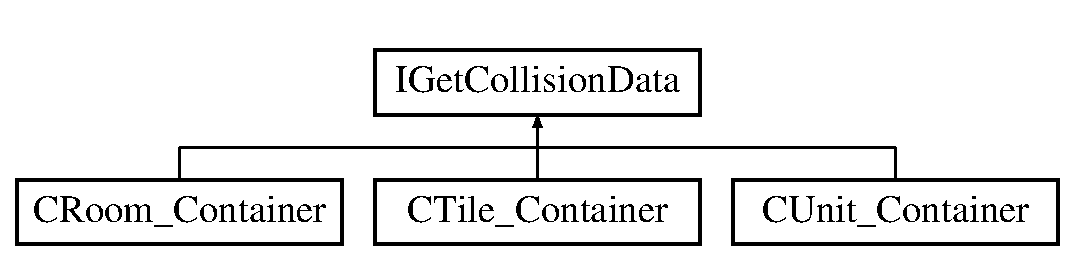
\includegraphics[height=2.000000cm]{classIGetCollisionData}
\end{center}
\end{figure}
\subsection*{Public Member Functions}
\begin{DoxyCompactItemize}
\item 
\hypertarget{classIGetCollisionData_a7b25012a7b2b296670467d03f105cf78}{virtual void {\bfseries get\-Collisiondata} (std\-::list$<$ \hyperlink{classARender}{A\-Render} $\ast$ $>$ $\ast$p\-List)=0}\label{classIGetCollisionData_a7b25012a7b2b296670467d03f105cf78}

\end{DoxyCompactItemize}


\subsection{Detailed Description}


Definition at line 14 of file I\-Get\-Collision\-Data.\-h.



The documentation for this class was generated from the following files\-:\begin{DoxyCompactItemize}
\item 
/home/z\-Zelman/\-Dropbox/\-Placeholder-\/\-R\-T\-S/src/\-Interfaces/I\-Get\-Collision\-Data.\-h\item 
/home/z\-Zelman/\-Dropbox/\-Placeholder-\/\-R\-T\-S/src/\-Interfaces/I\-Get\-Collision\-Data.\-cpp\end{DoxyCompactItemize}

\hypertarget{classIGetRenderData}{\section{I\-Get\-Render\-Data Class Reference}
\label{classIGetRenderData}\index{I\-Get\-Render\-Data@{I\-Get\-Render\-Data}}
}
Inheritance diagram for I\-Get\-Render\-Data\-:\begin{figure}[H]
\begin{center}
\leavevmode
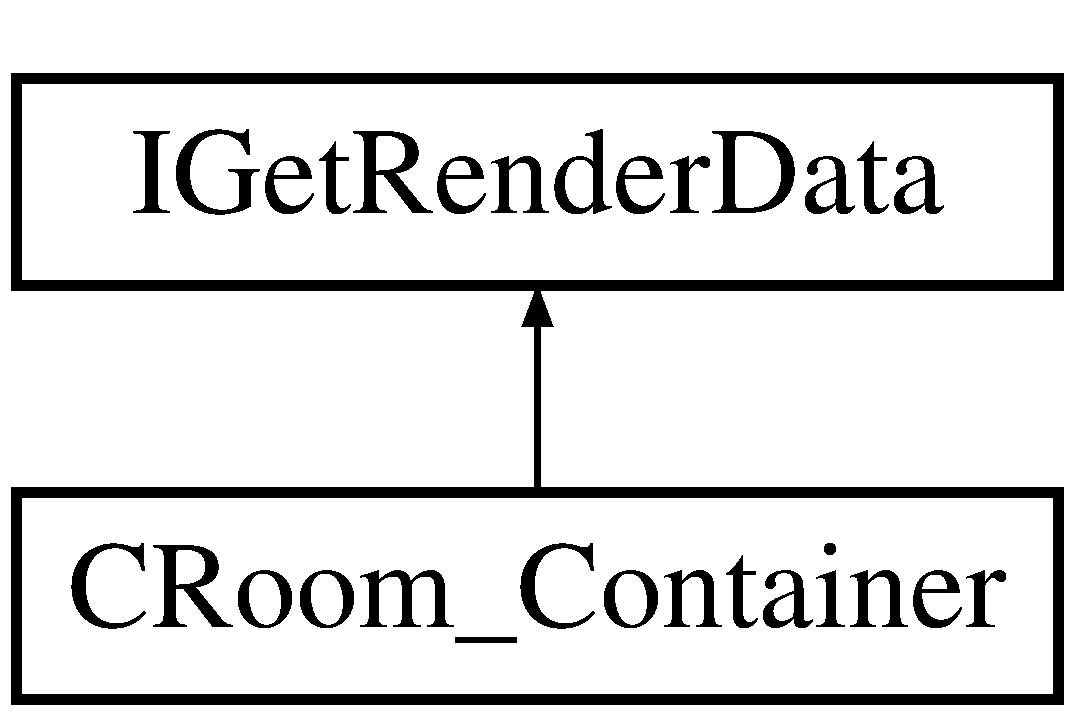
\includegraphics[height=2.000000cm]{classIGetRenderData}
\end{center}
\end{figure}
\subsection*{Public Member Functions}
\begin{DoxyCompactItemize}
\item 
\hypertarget{classIGetRenderData_aa128fd9ec5c5dc69e4db344dbba32aa2}{virtual void {\bfseries get\-Render\-Data} (std\-::list$<$ \hyperlink{classARender}{A\-Render} $\ast$ $>$ $\ast$p\-List)=0}\label{classIGetRenderData_aa128fd9ec5c5dc69e4db344dbba32aa2}

\end{DoxyCompactItemize}


\subsection{Detailed Description}


Definition at line 15 of file I\-Get\-Render\-Data.\-h.



The documentation for this class was generated from the following files\-:\begin{DoxyCompactItemize}
\item 
/home/z\-Zelman/\-Dropbox/\-Placeholder-\/\-R\-T\-S/src/\-Interfaces/I\-Get\-Render\-Data.\-h\item 
/home/z\-Zelman/\-Dropbox/\-Placeholder-\/\-R\-T\-S/src/\-Interfaces/I\-Get\-Render\-Data.\-cpp\end{DoxyCompactItemize}

\hypertarget{classsf_1_1Image}{\section{sf\-:\-:Image Class Reference}
\label{classsf_1_1Image}\index{sf\-::\-Image@{sf\-::\-Image}}
}


Class for loading, manipulating and saving images.  




{\ttfamily \#include $<$Image.\-hpp$>$}

\subsection*{Public Member Functions}
\begin{DoxyCompactItemize}
\item 
\hyperlink{classsf_1_1Image_abb4caf3cb167b613345ebe36fc883f12}{Image} ()
\begin{DoxyCompactList}\small\item\em Default constructor. \end{DoxyCompactList}\item 
void \hyperlink{classsf_1_1Image_a2a67930e2fd9ad97cf004e918cf5832b}{create} (unsigned int width, unsigned int height, const \hyperlink{classsf_1_1Color}{Color} \&color=\hyperlink{classsf_1_1Color}{Color}(0, 0, 0))
\begin{DoxyCompactList}\small\item\em Create the image and fill it with a unique color. \end{DoxyCompactList}\item 
void \hyperlink{classsf_1_1Image_a1c2b960ea12bdbb29e80934ce5268ebf}{create} (unsigned int width, unsigned int height, const Uint8 $\ast$pixels)
\begin{DoxyCompactList}\small\item\em Create the image from an array of pixels. \end{DoxyCompactList}\item 
bool \hyperlink{classsf_1_1Image_a9e4f2aa8e36d0cabde5ed5a4ef80290b}{load\-From\-File} (const std\-::string \&filename)
\begin{DoxyCompactList}\small\item\em Load the image from a file on disk. \end{DoxyCompactList}\item 
bool \hyperlink{classsf_1_1Image_aaa6c7afa5851a51cec6ab438faa7354c}{load\-From\-Memory} (const void $\ast$data, std\-::size\-\_\-t size)
\begin{DoxyCompactList}\small\item\em Load the image from a file in memory. \end{DoxyCompactList}\item 
bool \hyperlink{classsf_1_1Image_a21122ded0e8368bb06ed3b9acfbfb501}{load\-From\-Stream} (\hyperlink{classsf_1_1InputStream}{Input\-Stream} \&stream)
\begin{DoxyCompactList}\small\item\em Load the image from a custom stream. \end{DoxyCompactList}\item 
bool \hyperlink{classsf_1_1Image_aec0ed16b67df7b512aaa5c53388ba14e}{save\-To\-File} (const std\-::string \&filename) const 
\begin{DoxyCompactList}\small\item\em Save the image to a file on disk. \end{DoxyCompactList}\item 
\hyperlink{classsf_1_1Vector2}{Vector2u} \hyperlink{classsf_1_1Image_a5c3e9bebdc001c3ebf85ca97039fc86b}{get\-Size} () const 
\begin{DoxyCompactList}\small\item\em Return the size (width and height) of the image. \end{DoxyCompactList}\item 
void \hyperlink{classsf_1_1Image_a22f13f8c242a6b38eb73cc176b37ae34}{create\-Mask\-From\-Color} (const \hyperlink{classsf_1_1Color}{Color} \&color, Uint8 alpha=0)
\begin{DoxyCompactList}\small\item\em Create a transparency mask from a specified color-\/key. \end{DoxyCompactList}\item 
void \hyperlink{classsf_1_1Image_ab2fa337c956f85f93377dcb52153a45a}{copy} (const \hyperlink{classsf_1_1Image}{Image} \&source, unsigned int dest\-X, unsigned int dest\-Y, const \hyperlink{classsf_1_1Rect}{Int\-Rect} \&source\-Rect=\hyperlink{classsf_1_1Rect}{Int\-Rect}(0, 0, 0, 0), bool apply\-Alpha=false)
\begin{DoxyCompactList}\small\item\em Copy pixels from another image onto this one. \end{DoxyCompactList}\item 
void \hyperlink{classsf_1_1Image_a9fd329b8cd7d4439e07fb5d3bb2d9744}{set\-Pixel} (unsigned int x, unsigned int y, const \hyperlink{classsf_1_1Color}{Color} \&color)
\begin{DoxyCompactList}\small\item\em Change the color of a pixel. \end{DoxyCompactList}\item 
\hyperlink{classsf_1_1Color}{Color} \hyperlink{classsf_1_1Image_a8c8460e311dcb00557cb00a81c29163d}{get\-Pixel} (unsigned int x, unsigned int y) const 
\begin{DoxyCompactList}\small\item\em Get the color of a pixel. \end{DoxyCompactList}\item 
const Uint8 $\ast$ \hyperlink{classsf_1_1Image_ac6137a608a9efaae2735c13ff259c214}{get\-Pixels\-Ptr} () const 
\begin{DoxyCompactList}\small\item\em Get a read-\/only pointer to the array of pixels. \end{DoxyCompactList}\item 
\hypertarget{classsf_1_1Image_a57168e7bc29190e08bbd6c9c19f4bb2c}{void \hyperlink{classsf_1_1Image_a57168e7bc29190e08bbd6c9c19f4bb2c}{flip\-Horizontally} ()}\label{classsf_1_1Image_a57168e7bc29190e08bbd6c9c19f4bb2c}

\begin{DoxyCompactList}\small\item\em Flip the image horizontally (left $<$-\/$>$ right) \end{DoxyCompactList}\item 
\hypertarget{classsf_1_1Image_a78a702a7e49d1de2dec9894da99d279c}{void \hyperlink{classsf_1_1Image_a78a702a7e49d1de2dec9894da99d279c}{flip\-Vertically} ()}\label{classsf_1_1Image_a78a702a7e49d1de2dec9894da99d279c}

\begin{DoxyCompactList}\small\item\em Flip the image vertically (top $<$-\/$>$ bottom) \end{DoxyCompactList}\end{DoxyCompactItemize}


\subsection{Detailed Description}
Class for loading, manipulating and saving images. 

\hyperlink{classsf_1_1Image}{sf\-::\-Image} is an abstraction to manipulate images as bidimensional arrays of pixels. The class provides functions to load, read, write and save pixels, as well as many other useful functions.

\hyperlink{classsf_1_1Image}{sf\-::\-Image} can handle a unique internal representation of pixels, which is R\-G\-B\-A 32 bits. This means that a pixel must be composed of 8 bits red, green, blue and alpha channels -- just like a \hyperlink{classsf_1_1Color}{sf\-::\-Color}. All the functions that return an array of pixels follow this rule, and all parameters that you pass to \hyperlink{classsf_1_1Image}{sf\-::\-Image} functions (such as load\-From\-Pixels) must use this representation as well.

A \hyperlink{classsf_1_1Image}{sf\-::\-Image} can be copied, but it is a heavy resource and if possible you should always use \mbox{[}const\mbox{]} references to pass or return them to avoid useless copies.

Usage example\-: 
\begin{DoxyCode}
\textcolor{comment}{// Load an image file from a file}
\hyperlink{classsf_1_1Image}{sf::Image} background;
\textcolor{keywordflow}{if} (!background.\hyperlink{classsf_1_1Image_a9e4f2aa8e36d0cabde5ed5a4ef80290b}{loadFromFile}(\textcolor{stringliteral}{"background.jpg"}))
    \textcolor{keywordflow}{return} -1;

\textcolor{comment}{// Create a 20x20 image filled with black color}
\hyperlink{classsf_1_1Image}{sf::Image} image;
image.\hyperlink{classsf_1_1Image_a2a67930e2fd9ad97cf004e918cf5832b}{create}(20, 20, \hyperlink{classsf_1_1Color_a77c688197b981338f0b19dc58bd2facd}{sf::Color::Black});

\textcolor{comment}{// Copy image1 on image2 at position (10, 10)}
image.\hyperlink{classsf_1_1Image_ab2fa337c956f85f93377dcb52153a45a}{copy}(background, 10, 10);

\textcolor{comment}{// Make the top-left pixel transparent}
\hyperlink{classsf_1_1Color}{sf::Color} color = image.\hyperlink{classsf_1_1Image_a8c8460e311dcb00557cb00a81c29163d}{getPixel}(0, 0);
color.\hyperlink{classsf_1_1Color_a56dbdb47d5f040d9b78ac6a0b8b3a831}{a} = 0;
image.\hyperlink{classsf_1_1Image_a9fd329b8cd7d4439e07fb5d3bb2d9744}{setPixel}(0, 0, color);

\textcolor{comment}{// Save the image to a file}
\textcolor{keywordflow}{if} (!image.\hyperlink{classsf_1_1Image_aec0ed16b67df7b512aaa5c53388ba14e}{saveToFile}(\textcolor{stringliteral}{"result.png"}))
    \textcolor{keywordflow}{return} -1;
\end{DoxyCode}


\begin{DoxySeeAlso}{See Also}
\hyperlink{classsf_1_1Texture}{sf\-::\-Texture} 
\end{DoxySeeAlso}


Definition at line 46 of file Image.\-hpp.



\subsection{Constructor \& Destructor Documentation}
\hypertarget{classsf_1_1Image_abb4caf3cb167b613345ebe36fc883f12}{\index{sf\-::\-Image@{sf\-::\-Image}!Image@{Image}}
\index{Image@{Image}!sf::Image@{sf\-::\-Image}}
\subsubsection[{Image}]{\setlength{\rightskip}{0pt plus 5cm}sf\-::\-Image\-::\-Image (
\begin{DoxyParamCaption}
{}
\end{DoxyParamCaption}
)}}\label{classsf_1_1Image_abb4caf3cb167b613345ebe36fc883f12}


Default constructor. 

Creates an empty image. 

\subsection{Member Function Documentation}
\hypertarget{classsf_1_1Image_ab2fa337c956f85f93377dcb52153a45a}{\index{sf\-::\-Image@{sf\-::\-Image}!copy@{copy}}
\index{copy@{copy}!sf::Image@{sf\-::\-Image}}
\subsubsection[{copy}]{\setlength{\rightskip}{0pt plus 5cm}void sf\-::\-Image\-::copy (
\begin{DoxyParamCaption}
\item[{const {\bf Image} \&}]{source, }
\item[{unsigned int}]{dest\-X, }
\item[{unsigned int}]{dest\-Y, }
\item[{const {\bf Int\-Rect} \&}]{source\-Rect = {\ttfamily {\bf Int\-Rect}(0,~0,~0,~0)}, }
\item[{bool}]{apply\-Alpha = {\ttfamily false}}
\end{DoxyParamCaption}
)}}\label{classsf_1_1Image_ab2fa337c956f85f93377dcb52153a45a}


Copy pixels from another image onto this one. 

This function does a slow pixel copy and should not be used intensively. It can be used to prepare a complex static image from several others, but if you need this kind of feature in real-\/time you'd better use \hyperlink{classsf_1_1RenderTexture}{sf\-::\-Render\-Texture}.

If {\itshape source\-Rect} is empty, the whole image is copied. If {\itshape apply\-Alpha} is set to true, the transparency of source pixels is applied. If it is false, the pixels are copied unchanged with their alpha value.


\begin{DoxyParams}{Parameters}
{\em source} & Source image to copy \\
\hline
{\em dest\-X} & X coordinate of the destination position \\
\hline
{\em dest\-Y} & Y coordinate of the destination position \\
\hline
{\em source\-Rect} & Sub-\/rectangle of the source image to copy \\
\hline
{\em apply\-Alpha} & Should the copy take in account the source transparency? \\
\hline
\end{DoxyParams}
\hypertarget{classsf_1_1Image_a2a67930e2fd9ad97cf004e918cf5832b}{\index{sf\-::\-Image@{sf\-::\-Image}!create@{create}}
\index{create@{create}!sf::Image@{sf\-::\-Image}}
\subsubsection[{create}]{\setlength{\rightskip}{0pt plus 5cm}void sf\-::\-Image\-::create (
\begin{DoxyParamCaption}
\item[{unsigned int}]{width, }
\item[{unsigned int}]{height, }
\item[{const {\bf Color} \&}]{color = {\ttfamily {\bf Color}(0,~0,~0)}}
\end{DoxyParamCaption}
)}}\label{classsf_1_1Image_a2a67930e2fd9ad97cf004e918cf5832b}


Create the image and fill it with a unique color. 


\begin{DoxyParams}{Parameters}
{\em width} & Width of the image \\
\hline
{\em height} & Height of the image \\
\hline
{\em color} & Fill color \\
\hline
\end{DoxyParams}
\hypertarget{classsf_1_1Image_a1c2b960ea12bdbb29e80934ce5268ebf}{\index{sf\-::\-Image@{sf\-::\-Image}!create@{create}}
\index{create@{create}!sf::Image@{sf\-::\-Image}}
\subsubsection[{create}]{\setlength{\rightskip}{0pt plus 5cm}void sf\-::\-Image\-::create (
\begin{DoxyParamCaption}
\item[{unsigned int}]{width, }
\item[{unsigned int}]{height, }
\item[{const Uint8 $\ast$}]{pixels}
\end{DoxyParamCaption}
)}}\label{classsf_1_1Image_a1c2b960ea12bdbb29e80934ce5268ebf}


Create the image from an array of pixels. 

The {\itshape pixel} array is assumed to contain 32-\/bits R\-G\-B\-A pixels, and have the given {\itshape width} and {\itshape height}. If not, this is an undefined behaviour. If {\itshape pixels} is null, an empty image is created.


\begin{DoxyParams}{Parameters}
{\em width} & Width of the image \\
\hline
{\em height} & Height of the image \\
\hline
{\em pixels} & Array of pixels to copy to the image \\
\hline
\end{DoxyParams}
\hypertarget{classsf_1_1Image_a22f13f8c242a6b38eb73cc176b37ae34}{\index{sf\-::\-Image@{sf\-::\-Image}!create\-Mask\-From\-Color@{create\-Mask\-From\-Color}}
\index{create\-Mask\-From\-Color@{create\-Mask\-From\-Color}!sf::Image@{sf\-::\-Image}}
\subsubsection[{create\-Mask\-From\-Color}]{\setlength{\rightskip}{0pt plus 5cm}void sf\-::\-Image\-::create\-Mask\-From\-Color (
\begin{DoxyParamCaption}
\item[{const {\bf Color} \&}]{color, }
\item[{Uint8}]{alpha = {\ttfamily 0}}
\end{DoxyParamCaption}
)}}\label{classsf_1_1Image_a22f13f8c242a6b38eb73cc176b37ae34}


Create a transparency mask from a specified color-\/key. 

This function sets the alpha value of every pixel matching the given color to {\itshape alpha} (0 by default), so that they become transparent.


\begin{DoxyParams}{Parameters}
{\em color} & \hyperlink{classsf_1_1Color}{Color} to make transparent \\
\hline
{\em alpha} & Alpha value to assign to transparent pixels \\
\hline
\end{DoxyParams}
\hypertarget{classsf_1_1Image_a8c8460e311dcb00557cb00a81c29163d}{\index{sf\-::\-Image@{sf\-::\-Image}!get\-Pixel@{get\-Pixel}}
\index{get\-Pixel@{get\-Pixel}!sf::Image@{sf\-::\-Image}}
\subsubsection[{get\-Pixel}]{\setlength{\rightskip}{0pt plus 5cm}{\bf Color} sf\-::\-Image\-::get\-Pixel (
\begin{DoxyParamCaption}
\item[{unsigned int}]{x, }
\item[{unsigned int}]{y}
\end{DoxyParamCaption}
) const}}\label{classsf_1_1Image_a8c8460e311dcb00557cb00a81c29163d}


Get the color of a pixel. 

This function doesn't check the validity of the pixel coordinates, using out-\/of-\/range values will result in an undefined behaviour.


\begin{DoxyParams}{Parameters}
{\em x} & X coordinate of pixel to get \\
\hline
{\em y} & Y coordinate of pixel to get\\
\hline
\end{DoxyParams}
\begin{DoxyReturn}{Returns}
\hyperlink{classsf_1_1Color}{Color} of the pixel at coordinates (x, y)
\end{DoxyReturn}
\begin{DoxySeeAlso}{See Also}
\hyperlink{classsf_1_1Image_a9fd329b8cd7d4439e07fb5d3bb2d9744}{set\-Pixel} 
\end{DoxySeeAlso}
\hypertarget{classsf_1_1Image_ac6137a608a9efaae2735c13ff259c214}{\index{sf\-::\-Image@{sf\-::\-Image}!get\-Pixels\-Ptr@{get\-Pixels\-Ptr}}
\index{get\-Pixels\-Ptr@{get\-Pixels\-Ptr}!sf::Image@{sf\-::\-Image}}
\subsubsection[{get\-Pixels\-Ptr}]{\setlength{\rightskip}{0pt plus 5cm}const Uint8$\ast$ sf\-::\-Image\-::get\-Pixels\-Ptr (
\begin{DoxyParamCaption}
{}
\end{DoxyParamCaption}
) const}}\label{classsf_1_1Image_ac6137a608a9efaae2735c13ff259c214}


Get a read-\/only pointer to the array of pixels. 

The returned value points to an array of R\-G\-B\-A pixels made of 8 bits integers components. The size of the array is width $\ast$ height $\ast$ 4 (\hyperlink{classsf_1_1Image_a5c3e9bebdc001c3ebf85ca97039fc86b}{get\-Size()}.x $\ast$ \hyperlink{classsf_1_1Image_a5c3e9bebdc001c3ebf85ca97039fc86b}{get\-Size()}.y $\ast$ 4). Warning\-: the returned pointer may become invalid if you modify the image, so you should never store it for too long. If the image is empty, a null pointer is returned.

\begin{DoxyReturn}{Returns}
Read-\/only pointer to the array of pixels 
\end{DoxyReturn}
\hypertarget{classsf_1_1Image_a5c3e9bebdc001c3ebf85ca97039fc86b}{\index{sf\-::\-Image@{sf\-::\-Image}!get\-Size@{get\-Size}}
\index{get\-Size@{get\-Size}!sf::Image@{sf\-::\-Image}}
\subsubsection[{get\-Size}]{\setlength{\rightskip}{0pt plus 5cm}{\bf Vector2u} sf\-::\-Image\-::get\-Size (
\begin{DoxyParamCaption}
{}
\end{DoxyParamCaption}
) const}}\label{classsf_1_1Image_a5c3e9bebdc001c3ebf85ca97039fc86b}


Return the size (width and height) of the image. 

\begin{DoxyReturn}{Returns}
Size of the image, in pixels 
\end{DoxyReturn}
\hypertarget{classsf_1_1Image_a9e4f2aa8e36d0cabde5ed5a4ef80290b}{\index{sf\-::\-Image@{sf\-::\-Image}!load\-From\-File@{load\-From\-File}}
\index{load\-From\-File@{load\-From\-File}!sf::Image@{sf\-::\-Image}}
\subsubsection[{load\-From\-File}]{\setlength{\rightskip}{0pt plus 5cm}bool sf\-::\-Image\-::load\-From\-File (
\begin{DoxyParamCaption}
\item[{const std\-::string \&}]{filename}
\end{DoxyParamCaption}
)}}\label{classsf_1_1Image_a9e4f2aa8e36d0cabde5ed5a4ef80290b}


Load the image from a file on disk. 

The supported image formats are bmp, png, tga, jpg, gif, psd, hdr and pic. Some format options are not supported, like progressive jpeg. If this function fails, the image is left unchanged.


\begin{DoxyParams}{Parameters}
{\em filename} & Path of the image file to load\\
\hline
\end{DoxyParams}
\begin{DoxyReturn}{Returns}
True if loading was successful
\end{DoxyReturn}
\begin{DoxySeeAlso}{See Also}
\hyperlink{classsf_1_1Image_aaa6c7afa5851a51cec6ab438faa7354c}{load\-From\-Memory}, \hyperlink{classsf_1_1Image_a21122ded0e8368bb06ed3b9acfbfb501}{load\-From\-Stream}, \hyperlink{classsf_1_1Image_aec0ed16b67df7b512aaa5c53388ba14e}{save\-To\-File} 
\end{DoxySeeAlso}
\hypertarget{classsf_1_1Image_aaa6c7afa5851a51cec6ab438faa7354c}{\index{sf\-::\-Image@{sf\-::\-Image}!load\-From\-Memory@{load\-From\-Memory}}
\index{load\-From\-Memory@{load\-From\-Memory}!sf::Image@{sf\-::\-Image}}
\subsubsection[{load\-From\-Memory}]{\setlength{\rightskip}{0pt plus 5cm}bool sf\-::\-Image\-::load\-From\-Memory (
\begin{DoxyParamCaption}
\item[{const void $\ast$}]{data, }
\item[{std\-::size\-\_\-t}]{size}
\end{DoxyParamCaption}
)}}\label{classsf_1_1Image_aaa6c7afa5851a51cec6ab438faa7354c}


Load the image from a file in memory. 

The supported image formats are bmp, png, tga, jpg, gif, psd, hdr and pic. Some format options are not supported, like progressive jpeg. If this function fails, the image is left unchanged.


\begin{DoxyParams}{Parameters}
{\em data} & Pointer to the file data in memory \\
\hline
{\em size} & Size of the data to load, in bytes\\
\hline
\end{DoxyParams}
\begin{DoxyReturn}{Returns}
True if loading was successful
\end{DoxyReturn}
\begin{DoxySeeAlso}{See Also}
\hyperlink{classsf_1_1Image_a9e4f2aa8e36d0cabde5ed5a4ef80290b}{load\-From\-File}, \hyperlink{classsf_1_1Image_a21122ded0e8368bb06ed3b9acfbfb501}{load\-From\-Stream} 
\end{DoxySeeAlso}
\hypertarget{classsf_1_1Image_a21122ded0e8368bb06ed3b9acfbfb501}{\index{sf\-::\-Image@{sf\-::\-Image}!load\-From\-Stream@{load\-From\-Stream}}
\index{load\-From\-Stream@{load\-From\-Stream}!sf::Image@{sf\-::\-Image}}
\subsubsection[{load\-From\-Stream}]{\setlength{\rightskip}{0pt plus 5cm}bool sf\-::\-Image\-::load\-From\-Stream (
\begin{DoxyParamCaption}
\item[{{\bf Input\-Stream} \&}]{stream}
\end{DoxyParamCaption}
)}}\label{classsf_1_1Image_a21122ded0e8368bb06ed3b9acfbfb501}


Load the image from a custom stream. 

The supported image formats are bmp, png, tga, jpg, gif, psd, hdr and pic. Some format options are not supported, like progressive jpeg. If this function fails, the image is left unchanged.


\begin{DoxyParams}{Parameters}
{\em stream} & Source stream to read from\\
\hline
\end{DoxyParams}
\begin{DoxyReturn}{Returns}
True if loading was successful
\end{DoxyReturn}
\begin{DoxySeeAlso}{See Also}
\hyperlink{classsf_1_1Image_a9e4f2aa8e36d0cabde5ed5a4ef80290b}{load\-From\-File}, \hyperlink{classsf_1_1Image_aaa6c7afa5851a51cec6ab438faa7354c}{load\-From\-Memory} 
\end{DoxySeeAlso}
\hypertarget{classsf_1_1Image_aec0ed16b67df7b512aaa5c53388ba14e}{\index{sf\-::\-Image@{sf\-::\-Image}!save\-To\-File@{save\-To\-File}}
\index{save\-To\-File@{save\-To\-File}!sf::Image@{sf\-::\-Image}}
\subsubsection[{save\-To\-File}]{\setlength{\rightskip}{0pt plus 5cm}bool sf\-::\-Image\-::save\-To\-File (
\begin{DoxyParamCaption}
\item[{const std\-::string \&}]{filename}
\end{DoxyParamCaption}
) const}}\label{classsf_1_1Image_aec0ed16b67df7b512aaa5c53388ba14e}


Save the image to a file on disk. 

The format of the image is automatically deduced from the extension. The supported image formats are bmp, png, tga and jpg. The destination file is overwritten if it already exists. This function fails if the image is empty.


\begin{DoxyParams}{Parameters}
{\em filename} & Path of the file to save\\
\hline
\end{DoxyParams}
\begin{DoxyReturn}{Returns}
True if saving was successful
\end{DoxyReturn}
\begin{DoxySeeAlso}{See Also}
\hyperlink{classsf_1_1Image_a2a67930e2fd9ad97cf004e918cf5832b}{create}, \hyperlink{classsf_1_1Image_a9e4f2aa8e36d0cabde5ed5a4ef80290b}{load\-From\-File}, \hyperlink{classsf_1_1Image_aaa6c7afa5851a51cec6ab438faa7354c}{load\-From\-Memory} 
\end{DoxySeeAlso}
\hypertarget{classsf_1_1Image_a9fd329b8cd7d4439e07fb5d3bb2d9744}{\index{sf\-::\-Image@{sf\-::\-Image}!set\-Pixel@{set\-Pixel}}
\index{set\-Pixel@{set\-Pixel}!sf::Image@{sf\-::\-Image}}
\subsubsection[{set\-Pixel}]{\setlength{\rightskip}{0pt plus 5cm}void sf\-::\-Image\-::set\-Pixel (
\begin{DoxyParamCaption}
\item[{unsigned int}]{x, }
\item[{unsigned int}]{y, }
\item[{const {\bf Color} \&}]{color}
\end{DoxyParamCaption}
)}}\label{classsf_1_1Image_a9fd329b8cd7d4439e07fb5d3bb2d9744}


Change the color of a pixel. 

This function doesn't check the validity of the pixel coordinates, using out-\/of-\/range values will result in an undefined behaviour.


\begin{DoxyParams}{Parameters}
{\em x} & X coordinate of pixel to change \\
\hline
{\em y} & Y coordinate of pixel to change \\
\hline
{\em color} & New color of the pixel\\
\hline
\end{DoxyParams}
\begin{DoxySeeAlso}{See Also}
\hyperlink{classsf_1_1Image_a8c8460e311dcb00557cb00a81c29163d}{get\-Pixel} 
\end{DoxySeeAlso}


The documentation for this class was generated from the following file\-:\begin{DoxyCompactItemize}
\item 
/home/z\-Zelman/\-Dropbox/\-Placeholder-\/\-R\-T\-S/\-S\-F\-M\-L-\/2.\-1/include/\-S\-F\-M\-L/\-Graphics/Image.\-hpp\end{DoxyCompactItemize}

\hypertarget{classsf_1_1InputStream}{\section{sf\-:\-:Input\-Stream Class Reference}
\label{classsf_1_1InputStream}\index{sf\-::\-Input\-Stream@{sf\-::\-Input\-Stream}}
}


Abstract class for custom file input streams.  




{\ttfamily \#include $<$Input\-Stream.\-hpp$>$}

\subsection*{Public Member Functions}
\begin{DoxyCompactItemize}
\item 
\hypertarget{classsf_1_1InputStream_a4b2eb0f92323e630bd0542bc6191682e}{virtual \hyperlink{classsf_1_1InputStream_a4b2eb0f92323e630bd0542bc6191682e}{$\sim$\-Input\-Stream} ()}\label{classsf_1_1InputStream_a4b2eb0f92323e630bd0542bc6191682e}

\begin{DoxyCompactList}\small\item\em Virtual destructor. \end{DoxyCompactList}\item 
virtual Int64 \hyperlink{classsf_1_1InputStream_a8dd89c74c1acb693203f50e750c6ae53}{read} (void $\ast$data, Int64 size)=0
\begin{DoxyCompactList}\small\item\em Read data from the stream. \end{DoxyCompactList}\item 
virtual Int64 \hyperlink{classsf_1_1InputStream_a76aba8e5d5cf9b1c5902d5e04f7864fc}{seek} (Int64 position)=0
\begin{DoxyCompactList}\small\item\em Change the current reading position. \end{DoxyCompactList}\item 
virtual Int64 \hyperlink{classsf_1_1InputStream_a599515b9ccdbddb6fef5a98424fd559c}{tell} ()=0
\begin{DoxyCompactList}\small\item\em Get the current reading position in the stream. \end{DoxyCompactList}\item 
virtual Int64 \hyperlink{classsf_1_1InputStream_a311eaaaa65d636728e5153b574b72d5d}{get\-Size} ()=0
\begin{DoxyCompactList}\small\item\em Return the size of the stream. \end{DoxyCompactList}\end{DoxyCompactItemize}


\subsection{Detailed Description}
Abstract class for custom file input streams. 

This class allows users to define their own file input sources from which S\-F\-M\-L can load resources.

S\-F\-M\-L resource classes like \hyperlink{classsf_1_1Texture}{sf\-::\-Texture} and \hyperlink{classsf_1_1SoundBuffer}{sf\-::\-Sound\-Buffer} provide load\-From\-File and load\-From\-Memory functions, which read data from conventional sources. However, if you have data coming from a different source (over a network, embedded, encrypted, compressed, etc) you can derive your own class from \hyperlink{classsf_1_1InputStream}{sf\-::\-Input\-Stream} and load S\-F\-M\-L resources with their load\-From\-Stream function.

Usage example\-: 
\begin{DoxyCode}
\textcolor{comment}{// custom stream class that reads from inside a zip file}
\textcolor{keyword}{class }ZipStream : \textcolor{keyword}{public} \hyperlink{classsf_1_1InputStream}{sf::InputStream}
\{
\textcolor{keyword}{public} :

    ZipStream(std::string archive);

    \textcolor{keywordtype}{bool} open(std::string filename);

    Int64 \hyperlink{classsf_1_1InputStream_a8dd89c74c1acb693203f50e750c6ae53}{read}(\textcolor{keywordtype}{void}* data, Int64 size);

    Int64 \hyperlink{classsf_1_1InputStream_a76aba8e5d5cf9b1c5902d5e04f7864fc}{seek}(Int64 position);
    
    Int64 \hyperlink{classsf_1_1InputStream_a599515b9ccdbddb6fef5a98424fd559c}{tell}();

    Int64 \hyperlink{classsf_1_1InputStream_a311eaaaa65d636728e5153b574b72d5d}{getSize}();

\textcolor{keyword}{private} :

    ...
\};

\textcolor{comment}{// now you can load textures...}
\hyperlink{classsf_1_1Texture}{sf::Texture} texture;
ZipStream stream(\textcolor{stringliteral}{"resources.zip"});
stream.open(\textcolor{stringliteral}{"images/img.png"});
texture.\hyperlink{classsf_1_1Texture_a6803a13465a7113a8964d1081841886d}{loadFromStream}(stream);

\textcolor{comment}{// musics...}
\hyperlink{classsf_1_1Music}{sf::Music} music;
ZipStream stream(\textcolor{stringliteral}{"resources.zip"});
stream.open(\textcolor{stringliteral}{"musics/msc.ogg"});
music.\hyperlink{classsf_1_1Music_a4e55d1910a26858b44778c26b237d673}{openFromStream}(stream);

\textcolor{comment}{// etc.}
\end{DoxyCode}
 

Definition at line 40 of file Input\-Stream.\-hpp.



\subsection{Member Function Documentation}
\hypertarget{classsf_1_1InputStream_a311eaaaa65d636728e5153b574b72d5d}{\index{sf\-::\-Input\-Stream@{sf\-::\-Input\-Stream}!get\-Size@{get\-Size}}
\index{get\-Size@{get\-Size}!sf::InputStream@{sf\-::\-Input\-Stream}}
\subsubsection[{get\-Size}]{\setlength{\rightskip}{0pt plus 5cm}virtual Int64 sf\-::\-Input\-Stream\-::get\-Size (
\begin{DoxyParamCaption}
{}
\end{DoxyParamCaption}
)\hspace{0.3cm}{\ttfamily [pure virtual]}}}\label{classsf_1_1InputStream_a311eaaaa65d636728e5153b574b72d5d}


Return the size of the stream. 

\begin{DoxyReturn}{Returns}
The total number of bytes available in the stream, or -\/1 on error 
\end{DoxyReturn}
\hypertarget{classsf_1_1InputStream_a8dd89c74c1acb693203f50e750c6ae53}{\index{sf\-::\-Input\-Stream@{sf\-::\-Input\-Stream}!read@{read}}
\index{read@{read}!sf::InputStream@{sf\-::\-Input\-Stream}}
\subsubsection[{read}]{\setlength{\rightskip}{0pt plus 5cm}virtual Int64 sf\-::\-Input\-Stream\-::read (
\begin{DoxyParamCaption}
\item[{void $\ast$}]{data, }
\item[{Int64}]{size}
\end{DoxyParamCaption}
)\hspace{0.3cm}{\ttfamily [pure virtual]}}}\label{classsf_1_1InputStream_a8dd89c74c1acb693203f50e750c6ae53}


Read data from the stream. 

After reading, the stream's reading position must be advanced by the amount of bytes read.


\begin{DoxyParams}{Parameters}
{\em data} & Buffer where to copy the read data \\
\hline
{\em size} & Desired number of bytes to read\\
\hline
\end{DoxyParams}
\begin{DoxyReturn}{Returns}
The number of bytes actually read, or -\/1 on error 
\end{DoxyReturn}
\hypertarget{classsf_1_1InputStream_a76aba8e5d5cf9b1c5902d5e04f7864fc}{\index{sf\-::\-Input\-Stream@{sf\-::\-Input\-Stream}!seek@{seek}}
\index{seek@{seek}!sf::InputStream@{sf\-::\-Input\-Stream}}
\subsubsection[{seek}]{\setlength{\rightskip}{0pt plus 5cm}virtual Int64 sf\-::\-Input\-Stream\-::seek (
\begin{DoxyParamCaption}
\item[{Int64}]{position}
\end{DoxyParamCaption}
)\hspace{0.3cm}{\ttfamily [pure virtual]}}}\label{classsf_1_1InputStream_a76aba8e5d5cf9b1c5902d5e04f7864fc}


Change the current reading position. 


\begin{DoxyParams}{Parameters}
{\em position} & The position to seek to, from the beginning\\
\hline
\end{DoxyParams}
\begin{DoxyReturn}{Returns}
The position actually sought to, or -\/1 on error 
\end{DoxyReturn}
\hypertarget{classsf_1_1InputStream_a599515b9ccdbddb6fef5a98424fd559c}{\index{sf\-::\-Input\-Stream@{sf\-::\-Input\-Stream}!tell@{tell}}
\index{tell@{tell}!sf::InputStream@{sf\-::\-Input\-Stream}}
\subsubsection[{tell}]{\setlength{\rightskip}{0pt plus 5cm}virtual Int64 sf\-::\-Input\-Stream\-::tell (
\begin{DoxyParamCaption}
{}
\end{DoxyParamCaption}
)\hspace{0.3cm}{\ttfamily [pure virtual]}}}\label{classsf_1_1InputStream_a599515b9ccdbddb6fef5a98424fd559c}


Get the current reading position in the stream. 

\begin{DoxyReturn}{Returns}
The current position, or -\/1 on error. 
\end{DoxyReturn}


The documentation for this class was generated from the following file\-:\begin{DoxyCompactItemize}
\item 
/home/z\-Zelman/\-Dropbox/\-Placeholder-\/\-R\-T\-S/\-S\-F\-M\-L-\/2.\-1/include/\-S\-F\-M\-L/\-System/Input\-Stream.\-hpp\end{DoxyCompactItemize}

\hypertarget{classsf_1_1IpAddress}{\section{sf\-:\-:Ip\-Address Class Reference}
\label{classsf_1_1IpAddress}\index{sf\-::\-Ip\-Address@{sf\-::\-Ip\-Address}}
}


Encapsulate an I\-Pv4 network address.  




{\ttfamily \#include $<$Ip\-Address.\-hpp$>$}

\subsection*{Public Member Functions}
\begin{DoxyCompactItemize}
\item 
\hyperlink{classsf_1_1IpAddress_af32a0574baa0f46e48deb2d83ca7658b}{Ip\-Address} ()
\begin{DoxyCompactList}\small\item\em Default constructor. \end{DoxyCompactList}\item 
\hyperlink{classsf_1_1IpAddress_a656b7445ab04cabaa7398685bc09c3f7}{Ip\-Address} (const std\-::string \&address)
\begin{DoxyCompactList}\small\item\em Construct the address from a string. \end{DoxyCompactList}\item 
\hyperlink{classsf_1_1IpAddress_a92f2a9be74334a61b96c2fc79fe6eb78}{Ip\-Address} (const char $\ast$address)
\begin{DoxyCompactList}\small\item\em Construct the address from a string. \end{DoxyCompactList}\item 
\hyperlink{classsf_1_1IpAddress_a1d289dcb9ce7a64c600c6f84cba88cc6}{Ip\-Address} (Uint8 byte0, Uint8 byte1, Uint8 byte2, Uint8 byte3)
\begin{DoxyCompactList}\small\item\em Construct the address from 4 bytes. \end{DoxyCompactList}\item 
\hyperlink{classsf_1_1IpAddress_a8ed34ba3a40d70eb9f09ac5ae779a162}{Ip\-Address} (Uint32 address)
\begin{DoxyCompactList}\small\item\em Construct the address from a 32-\/bits integer. \end{DoxyCompactList}\item 
std\-::string \hyperlink{classsf_1_1IpAddress_a52f4be92fb0ceb689abc469e4a85fd82}{to\-String} () const 
\begin{DoxyCompactList}\small\item\em Get a string representation of the address. \end{DoxyCompactList}\item 
Uint32 \hyperlink{classsf_1_1IpAddress_af42678b08b23def2560aed7d98b24d89}{to\-Integer} () const 
\begin{DoxyCompactList}\small\item\em Get an integer representation of the address. \end{DoxyCompactList}\end{DoxyCompactItemize}
\subsection*{Static Public Member Functions}
\begin{DoxyCompactItemize}
\item 
static \hyperlink{classsf_1_1IpAddress}{Ip\-Address} \hyperlink{classsf_1_1IpAddress_a4c31622ad87edca48adbb8e8ed00ee4a}{get\-Local\-Address} ()
\begin{DoxyCompactList}\small\item\em Get the computer's local address. \end{DoxyCompactList}\item 
static \hyperlink{classsf_1_1IpAddress}{Ip\-Address} \hyperlink{classsf_1_1IpAddress_a5c5cbf67e4aacf23c24f2ad991df4c55}{get\-Public\-Address} (\hyperlink{classsf_1_1Time}{Time} timeout=\hyperlink{classsf_1_1Time_a8db127b632fa8da21550e7282af11fa0}{Time\-::\-Zero})
\begin{DoxyCompactList}\small\item\em Get the computer's public address. \end{DoxyCompactList}\end{DoxyCompactItemize}
\subsection*{Static Public Attributes}
\begin{DoxyCompactItemize}
\item 
\hypertarget{classsf_1_1IpAddress_a4619b4abbe3c8fef056e7299db967404}{static const \hyperlink{classsf_1_1IpAddress}{Ip\-Address} \hyperlink{classsf_1_1IpAddress_a4619b4abbe3c8fef056e7299db967404}{None}}\label{classsf_1_1IpAddress_a4619b4abbe3c8fef056e7299db967404}

\begin{DoxyCompactList}\small\item\em Value representing an empty/invalid address. \end{DoxyCompactList}\item 
\hypertarget{classsf_1_1IpAddress_a594d3a8e2559f8fa8ab0a96fa597333b}{static const \hyperlink{classsf_1_1IpAddress}{Ip\-Address} \hyperlink{classsf_1_1IpAddress_a594d3a8e2559f8fa8ab0a96fa597333b}{Local\-Host}}\label{classsf_1_1IpAddress_a594d3a8e2559f8fa8ab0a96fa597333b}

\begin{DoxyCompactList}\small\item\em The \char`\"{}localhost\char`\"{} address (for connecting a computer to itself locally) \end{DoxyCompactList}\item 
\hypertarget{classsf_1_1IpAddress_aa93d1d57b65d243f2baf804b6035465c}{static const \hyperlink{classsf_1_1IpAddress}{Ip\-Address} \hyperlink{classsf_1_1IpAddress_aa93d1d57b65d243f2baf804b6035465c}{Broadcast}}\label{classsf_1_1IpAddress_aa93d1d57b65d243f2baf804b6035465c}

\begin{DoxyCompactList}\small\item\em The \char`\"{}broadcast\char`\"{} address (for sending U\-D\-P messages to everyone on a local network) \end{DoxyCompactList}\end{DoxyCompactItemize}


\subsection{Detailed Description}
Encapsulate an I\-Pv4 network address. 

\hyperlink{classsf_1_1IpAddress}{sf\-::\-Ip\-Address} is a utility class for manipulating network addresses. It provides a set a implicit constructors and conversion functions to easily build or transform an I\-P address from/to various representations.

Usage example\-: 
\begin{DoxyCode}
\hyperlink{classsf_1_1IpAddress}{sf::IpAddress} a0;                                     \textcolor{comment}{// an invalid address}
\hyperlink{classsf_1_1IpAddress}{sf::IpAddress} a1 = \hyperlink{classsf_1_1IpAddress_a4619b4abbe3c8fef056e7299db967404}{sf::IpAddress::None};               \textcolor{comment}{// an invalid address
       (same as a0)}
\hyperlink{classsf_1_1IpAddress}{sf::IpAddress} a2(\textcolor{stringliteral}{"127.0.0.1"});                        \textcolor{comment}{// the local host address}
\hyperlink{classsf_1_1IpAddress}{sf::IpAddress} a3 = \hyperlink{classsf_1_1IpAddress_aa93d1d57b65d243f2baf804b6035465c}{sf::IpAddress::Broadcast};          \textcolor{comment}{// the broadcast
       address}
\hyperlink{classsf_1_1IpAddress}{sf::IpAddress} a4(192, 168, 1, 56);                    \textcolor{comment}{// a local address}
\hyperlink{classsf_1_1IpAddress}{sf::IpAddress} a5(\textcolor{stringliteral}{"my\_computer"});                      \textcolor{comment}{// a local address created from a
       network name}
\hyperlink{classsf_1_1IpAddress}{sf::IpAddress} a6(\textcolor{stringliteral}{"89.54.1.169"});                      \textcolor{comment}{// a distant address}
\hyperlink{classsf_1_1IpAddress}{sf::IpAddress} a7(\textcolor{stringliteral}{"www.google.com"});                   \textcolor{comment}{// a distant address created from a
       network name}
\hyperlink{classsf_1_1IpAddress}{sf::IpAddress} a8 = \hyperlink{classsf_1_1IpAddress_a4c31622ad87edca48adbb8e8ed00ee4a}{sf::IpAddress::getLocalAddress}();  \textcolor{comment}{// my
       address on the local network}
\hyperlink{classsf_1_1IpAddress}{sf::IpAddress} a9 = \hyperlink{classsf_1_1IpAddress_a5c5cbf67e4aacf23c24f2ad991df4c55}{sf::IpAddress::getPublicAddress}(); \textcolor{comment}{// my
       address on the internet}
\end{DoxyCode}


Note that \hyperlink{classsf_1_1IpAddress}{sf\-::\-Ip\-Address} currently doesn't support I\-Pv6 nor other types of network addresses. 

Definition at line 44 of file Ip\-Address.\-hpp.



\subsection{Constructor \& Destructor Documentation}
\hypertarget{classsf_1_1IpAddress_af32a0574baa0f46e48deb2d83ca7658b}{\index{sf\-::\-Ip\-Address@{sf\-::\-Ip\-Address}!Ip\-Address@{Ip\-Address}}
\index{Ip\-Address@{Ip\-Address}!sf::IpAddress@{sf\-::\-Ip\-Address}}
\subsubsection[{Ip\-Address}]{\setlength{\rightskip}{0pt plus 5cm}sf\-::\-Ip\-Address\-::\-Ip\-Address (
\begin{DoxyParamCaption}
{}
\end{DoxyParamCaption}
)}}\label{classsf_1_1IpAddress_af32a0574baa0f46e48deb2d83ca7658b}


Default constructor. 

This constructor creates an empty (invalid) address \hypertarget{classsf_1_1IpAddress_a656b7445ab04cabaa7398685bc09c3f7}{\index{sf\-::\-Ip\-Address@{sf\-::\-Ip\-Address}!Ip\-Address@{Ip\-Address}}
\index{Ip\-Address@{Ip\-Address}!sf::IpAddress@{sf\-::\-Ip\-Address}}
\subsubsection[{Ip\-Address}]{\setlength{\rightskip}{0pt plus 5cm}sf\-::\-Ip\-Address\-::\-Ip\-Address (
\begin{DoxyParamCaption}
\item[{const std\-::string \&}]{address}
\end{DoxyParamCaption}
)}}\label{classsf_1_1IpAddress_a656b7445ab04cabaa7398685bc09c3f7}


Construct the address from a string. 

Here {\itshape address} can be either a decimal address (ex\-: \char`\"{}192.\-168.\-1.\-56\char`\"{}) or a network name (ex\-: \char`\"{}localhost\char`\"{}).


\begin{DoxyParams}{Parameters}
{\em address} & I\-P address or network name \\
\hline
\end{DoxyParams}
\hypertarget{classsf_1_1IpAddress_a92f2a9be74334a61b96c2fc79fe6eb78}{\index{sf\-::\-Ip\-Address@{sf\-::\-Ip\-Address}!Ip\-Address@{Ip\-Address}}
\index{Ip\-Address@{Ip\-Address}!sf::IpAddress@{sf\-::\-Ip\-Address}}
\subsubsection[{Ip\-Address}]{\setlength{\rightskip}{0pt plus 5cm}sf\-::\-Ip\-Address\-::\-Ip\-Address (
\begin{DoxyParamCaption}
\item[{const char $\ast$}]{address}
\end{DoxyParamCaption}
)}}\label{classsf_1_1IpAddress_a92f2a9be74334a61b96c2fc79fe6eb78}


Construct the address from a string. 

Here {\itshape address} can be either a decimal address (ex\-: \char`\"{}192.\-168.\-1.\-56\char`\"{}) or a network name (ex\-: \char`\"{}localhost\char`\"{}). This is equivalent to the constructor taking a std\-::string parameter, it is defined for convenience so that the implicit conversions from literal strings to \hyperlink{classsf_1_1IpAddress}{Ip\-Address} work.


\begin{DoxyParams}{Parameters}
{\em address} & I\-P address or network name \\
\hline
\end{DoxyParams}
\hypertarget{classsf_1_1IpAddress_a1d289dcb9ce7a64c600c6f84cba88cc6}{\index{sf\-::\-Ip\-Address@{sf\-::\-Ip\-Address}!Ip\-Address@{Ip\-Address}}
\index{Ip\-Address@{Ip\-Address}!sf::IpAddress@{sf\-::\-Ip\-Address}}
\subsubsection[{Ip\-Address}]{\setlength{\rightskip}{0pt plus 5cm}sf\-::\-Ip\-Address\-::\-Ip\-Address (
\begin{DoxyParamCaption}
\item[{Uint8}]{byte0, }
\item[{Uint8}]{byte1, }
\item[{Uint8}]{byte2, }
\item[{Uint8}]{byte3}
\end{DoxyParamCaption}
)}}\label{classsf_1_1IpAddress_a1d289dcb9ce7a64c600c6f84cba88cc6}


Construct the address from 4 bytes. 

Calling Ip\-Address(a, b, c, d) is equivalent to calling \hyperlink{classsf_1_1IpAddress}{Ip\-Address}(\char`\"{}a.\-b.\-c.\-d\char`\"{}), but safer as it doesn't have to parse a string to get the address components.


\begin{DoxyParams}{Parameters}
{\em byte0} & First byte of the address \\
\hline
{\em byte1} & Second byte of the address \\
\hline
{\em byte2} & Third byte of the address \\
\hline
{\em byte3} & Fourth byte of the address \\
\hline
\end{DoxyParams}
\hypertarget{classsf_1_1IpAddress_a8ed34ba3a40d70eb9f09ac5ae779a162}{\index{sf\-::\-Ip\-Address@{sf\-::\-Ip\-Address}!Ip\-Address@{Ip\-Address}}
\index{Ip\-Address@{Ip\-Address}!sf::IpAddress@{sf\-::\-Ip\-Address}}
\subsubsection[{Ip\-Address}]{\setlength{\rightskip}{0pt plus 5cm}sf\-::\-Ip\-Address\-::\-Ip\-Address (
\begin{DoxyParamCaption}
\item[{Uint32}]{address}
\end{DoxyParamCaption}
)\hspace{0.3cm}{\ttfamily [explicit]}}}\label{classsf_1_1IpAddress_a8ed34ba3a40d70eb9f09ac5ae779a162}


Construct the address from a 32-\/bits integer. 

This constructor uses the internal representation of the address directly. It should be used for optimization purposes, and only if you got that representation from Ip\-Address\-::\-To\-Integer().


\begin{DoxyParams}{Parameters}
{\em address} & 4 bytes of the address packed into a 32-\/bits integer\\
\hline
\end{DoxyParams}
\begin{DoxySeeAlso}{See Also}
\hyperlink{classsf_1_1IpAddress_af42678b08b23def2560aed7d98b24d89}{to\-Integer} 
\end{DoxySeeAlso}


\subsection{Member Function Documentation}
\hypertarget{classsf_1_1IpAddress_a4c31622ad87edca48adbb8e8ed00ee4a}{\index{sf\-::\-Ip\-Address@{sf\-::\-Ip\-Address}!get\-Local\-Address@{get\-Local\-Address}}
\index{get\-Local\-Address@{get\-Local\-Address}!sf::IpAddress@{sf\-::\-Ip\-Address}}
\subsubsection[{get\-Local\-Address}]{\setlength{\rightskip}{0pt plus 5cm}static {\bf Ip\-Address} sf\-::\-Ip\-Address\-::get\-Local\-Address (
\begin{DoxyParamCaption}
{}
\end{DoxyParamCaption}
)\hspace{0.3cm}{\ttfamily [static]}}}\label{classsf_1_1IpAddress_a4c31622ad87edca48adbb8e8ed00ee4a}


Get the computer's local address. 

The local address is the address of the computer from the L\-A\-N point of view, i.\-e. something like 192.\-168.\-1.\-56. It is meaningful only for communications over the local network. Unlike get\-Public\-Address, this function is fast and may be used safely anywhere.

\begin{DoxyReturn}{Returns}
Local I\-P address of the computer
\end{DoxyReturn}
\begin{DoxySeeAlso}{See Also}
\hyperlink{classsf_1_1IpAddress_a5c5cbf67e4aacf23c24f2ad991df4c55}{get\-Public\-Address} 
\end{DoxySeeAlso}
\hypertarget{classsf_1_1IpAddress_a5c5cbf67e4aacf23c24f2ad991df4c55}{\index{sf\-::\-Ip\-Address@{sf\-::\-Ip\-Address}!get\-Public\-Address@{get\-Public\-Address}}
\index{get\-Public\-Address@{get\-Public\-Address}!sf::IpAddress@{sf\-::\-Ip\-Address}}
\subsubsection[{get\-Public\-Address}]{\setlength{\rightskip}{0pt plus 5cm}static {\bf Ip\-Address} sf\-::\-Ip\-Address\-::get\-Public\-Address (
\begin{DoxyParamCaption}
\item[{{\bf Time}}]{timeout = {\ttfamily {\bf Time\-::\-Zero}}}
\end{DoxyParamCaption}
)\hspace{0.3cm}{\ttfamily [static]}}}\label{classsf_1_1IpAddress_a5c5cbf67e4aacf23c24f2ad991df4c55}


Get the computer's public address. 

The public address is the address of the computer from the internet point of view, i.\-e. something like 89.\-54.\-1.\-169. It is necessary for communications over the world wide web. The only way to get a public address is to ask it to a distant website; as a consequence, this function depends on both your network connection and the server, and may be very slow. You should use it as few as possible. Because this function depends on the network connection and on a distant server, you may use a time limit if you don't want your program to be possibly stuck waiting in case there is a problem; this limit is deactivated by default.


\begin{DoxyParams}{Parameters}
{\em timeout} & Maximum time to wait\\
\hline
\end{DoxyParams}
\begin{DoxyReturn}{Returns}
Public I\-P address of the computer
\end{DoxyReturn}
\begin{DoxySeeAlso}{See Also}
\hyperlink{classsf_1_1IpAddress_a4c31622ad87edca48adbb8e8ed00ee4a}{get\-Local\-Address} 
\end{DoxySeeAlso}
\hypertarget{classsf_1_1IpAddress_af42678b08b23def2560aed7d98b24d89}{\index{sf\-::\-Ip\-Address@{sf\-::\-Ip\-Address}!to\-Integer@{to\-Integer}}
\index{to\-Integer@{to\-Integer}!sf::IpAddress@{sf\-::\-Ip\-Address}}
\subsubsection[{to\-Integer}]{\setlength{\rightskip}{0pt plus 5cm}Uint32 sf\-::\-Ip\-Address\-::to\-Integer (
\begin{DoxyParamCaption}
{}
\end{DoxyParamCaption}
) const}}\label{classsf_1_1IpAddress_af42678b08b23def2560aed7d98b24d89}


Get an integer representation of the address. 

The returned number is the internal representation of the address, and should be used for optimization purposes only (like sending the address through a socket). The integer produced by this function can then be converted back to a \hyperlink{classsf_1_1IpAddress}{sf\-::\-Ip\-Address} with the proper constructor.

\begin{DoxyReturn}{Returns}
32-\/bits unsigned integer representation of the address
\end{DoxyReturn}
\begin{DoxySeeAlso}{See Also}
\hyperlink{classsf_1_1IpAddress_a52f4be92fb0ceb689abc469e4a85fd82}{to\-String} 
\end{DoxySeeAlso}
\hypertarget{classsf_1_1IpAddress_a52f4be92fb0ceb689abc469e4a85fd82}{\index{sf\-::\-Ip\-Address@{sf\-::\-Ip\-Address}!to\-String@{to\-String}}
\index{to\-String@{to\-String}!sf::IpAddress@{sf\-::\-Ip\-Address}}
\subsubsection[{to\-String}]{\setlength{\rightskip}{0pt plus 5cm}std\-::string sf\-::\-Ip\-Address\-::to\-String (
\begin{DoxyParamCaption}
{}
\end{DoxyParamCaption}
) const}}\label{classsf_1_1IpAddress_a52f4be92fb0ceb689abc469e4a85fd82}


Get a string representation of the address. 

The returned string is the decimal representation of the I\-P address (like \char`\"{}192.\-168.\-1.\-56\char`\"{}), even if it was constructed from a host name.

\begin{DoxyReturn}{Returns}
\hyperlink{classsf_1_1String}{String} representation of the address
\end{DoxyReturn}
\begin{DoxySeeAlso}{See Also}
\hyperlink{classsf_1_1IpAddress_af42678b08b23def2560aed7d98b24d89}{to\-Integer} 
\end{DoxySeeAlso}


The documentation for this class was generated from the following file\-:\begin{DoxyCompactItemize}
\item 
/home/z\-Zelman/\-Dropbox/\-Placeholder-\/\-R\-T\-S/\-S\-F\-M\-L-\/2.\-1/include/\-S\-F\-M\-L/\-Network/Ip\-Address.\-hpp\end{DoxyCompactItemize}

\hypertarget{classIUpdateable}{\section{I\-Updateable Class Reference}
\label{classIUpdateable}\index{I\-Updateable@{I\-Updateable}}
}
Inheritance diagram for I\-Updateable\-:\begin{figure}[H]
\begin{center}
\leavevmode
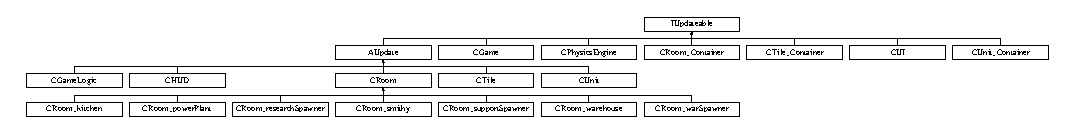
\includegraphics[height=1.333333cm]{classIUpdateable}
\end{center}
\end{figure}
\subsection*{Public Member Functions}
\begin{DoxyCompactItemize}
\item 
\hypertarget{classIUpdateable_a46d178a1ecdab33bcaad25d9b38582a5}{virtual void {\bfseries update} ()=0}\label{classIUpdateable_a46d178a1ecdab33bcaad25d9b38582a5}

\end{DoxyCompactItemize}


\subsection{Detailed Description}


Definition at line 12 of file I\-Updateable.\-h.



The documentation for this class was generated from the following files\-:\begin{DoxyCompactItemize}
\item 
/home/z\-Zelman/\-Dropbox/\-Placeholder-\/\-R\-T\-S/src/\-Interfaces/I\-Updateable.\-h\item 
/home/z\-Zelman/\-Dropbox/\-Placeholder-\/\-R\-T\-S/src/\-Interfaces/I\-Updateable.\-cpp\end{DoxyCompactItemize}

\hypertarget{classsf_1_1Joystick}{\section{sf\-:\-:Joystick Class Reference}
\label{classsf_1_1Joystick}\index{sf\-::\-Joystick@{sf\-::\-Joystick}}
}


Give access to the real-\/time state of the joysticks.  




{\ttfamily \#include $<$Joystick.\-hpp$>$}

\subsection*{Public Types}
\begin{DoxyCompactItemize}
\item 
enum \{ \hyperlink{classsf_1_1Joystick_a951a7c775921304a5f3443c6e2bb4d65a6e0a2a95bc1da277610c04d80f52715e}{Count} = 8, 
\hyperlink{classsf_1_1Joystick_a951a7c775921304a5f3443c6e2bb4d65a2f1b8a0a59f2c12a4775c0e1e69e1816}{Button\-Count} = 32, 
\hyperlink{classsf_1_1Joystick_a951a7c775921304a5f3443c6e2bb4d65accf3e487c9f6ee2f384351323626a42c}{Axis\-Count} = 8
 \}
\begin{DoxyCompactList}\small\item\em Constants related to joysticks capabilities. \end{DoxyCompactList}\item 
enum \hyperlink{classsf_1_1Joystick_a48db337092c2e263774f94de6d50baa7}{Axis} \{ \\*
\hyperlink{classsf_1_1Joystick_a48db337092c2e263774f94de6d50baa7a95dc8b9bf7b0a2157fc67891c54c401e}{X}, 
\hyperlink{classsf_1_1Joystick_a48db337092c2e263774f94de6d50baa7a51ef1455f7511ad4a78ba241d66593ce}{Y}, 
\hyperlink{classsf_1_1Joystick_a48db337092c2e263774f94de6d50baa7a7c37a1240b2dafbbfc5c1a0e23911315}{Z}, 
\hyperlink{classsf_1_1Joystick_a48db337092c2e263774f94de6d50baa7aeebbcdb0828850f4d69e6a084801fab8}{R}, 
\\*
\hyperlink{classsf_1_1Joystick_a48db337092c2e263774f94de6d50baa7a0a901f61e75292dd2f642b6e4f33a214}{U}, 
\hyperlink{classsf_1_1Joystick_a48db337092c2e263774f94de6d50baa7aa2e2c8ffa1837e7911ee0c7d045bf8f4}{V}, 
\hyperlink{classsf_1_1Joystick_a48db337092c2e263774f94de6d50baa7a06420f7714e4dfd8b841885a0b5f3954}{Pov\-X}, 
\hyperlink{classsf_1_1Joystick_a48db337092c2e263774f94de6d50baa7a0f8ffb2dcddf91b98ab910a4f8327ad9}{Pov\-Y}
 \}
\begin{DoxyCompactList}\small\item\em Axes supported by S\-F\-M\-L joysticks. \end{DoxyCompactList}\end{DoxyCompactItemize}
\subsection*{Static Public Member Functions}
\begin{DoxyCompactItemize}
\item 
static bool \hyperlink{classsf_1_1Joystick_ac7d4e1923e9f9420174f26703ea63d6c}{is\-Connected} (unsigned int joystick)
\begin{DoxyCompactList}\small\item\em Check if a joystick is connected. \end{DoxyCompactList}\item 
static unsigned int \hyperlink{classsf_1_1Joystick_a4de9f445c6582bfe9f0873f695682885}{get\-Button\-Count} (unsigned int joystick)
\begin{DoxyCompactList}\small\item\em Return the number of buttons supported by a joystick. \end{DoxyCompactList}\item 
static bool \hyperlink{classsf_1_1Joystick_a268e8f2a11ae6af4a47c727cb4ab4d95}{has\-Axis} (unsigned int joystick, \hyperlink{classsf_1_1Joystick_a48db337092c2e263774f94de6d50baa7}{Axis} axis)
\begin{DoxyCompactList}\small\item\em Check if a joystick supports a given axis. \end{DoxyCompactList}\item 
static bool \hyperlink{classsf_1_1Joystick_ae0d97a4b84268cbe6a7078e1b2717835}{is\-Button\-Pressed} (unsigned int joystick, unsigned int button)
\begin{DoxyCompactList}\small\item\em Check if a joystick button is pressed. \end{DoxyCompactList}\item 
static float \hyperlink{classsf_1_1Joystick_aea4930193331df1851b709f3060ba58b}{get\-Axis\-Position} (unsigned int joystick, \hyperlink{classsf_1_1Joystick_a48db337092c2e263774f94de6d50baa7}{Axis} axis)
\begin{DoxyCompactList}\small\item\em Get the current position of a joystick axis. \end{DoxyCompactList}\item 
static void \hyperlink{classsf_1_1Joystick_ab85fa9175b4edd3e5a07ee3cde0b0f48}{update} ()
\begin{DoxyCompactList}\small\item\em Update the states of all joysticks. \end{DoxyCompactList}\end{DoxyCompactItemize}


\subsection{Detailed Description}
Give access to the real-\/time state of the joysticks. 

\hyperlink{classsf_1_1Joystick}{sf\-::\-Joystick} provides an interface to the state of the joysticks. It only contains static functions, so it's not meant to be instanciated. Instead, each joystick is identified by an index that is passed to the functions of this class.

This class allows users to query the state of joysticks at any time and directly, without having to deal with a window and its events. Compared to the Joystick\-Moved, Joystick\-Button\-Pressed and Joystick\-Button\-Released events, \hyperlink{classsf_1_1Joystick}{sf\-::\-Joystick} can retrieve the state of axes and buttons of joysticks at any time (you don't need to store and update a boolean on your side in order to know if a button is pressed or released), and you always get the real state of joysticks, even if they are moved, pressed or released when your window is out of focus and no event is triggered.

S\-F\-M\-L supports\-: \begin{DoxyItemize}
\item 8 joysticks (\hyperlink{classsf_1_1Joystick_a951a7c775921304a5f3443c6e2bb4d65a6e0a2a95bc1da277610c04d80f52715e}{sf\-::\-Joystick\-::\-Count}) \item 32 buttons per joystick (\hyperlink{classsf_1_1Joystick_a951a7c775921304a5f3443c6e2bb4d65a2f1b8a0a59f2c12a4775c0e1e69e1816}{sf\-::\-Joystick\-::\-Button\-Count}) \item 8 axes per joystick (\hyperlink{classsf_1_1Joystick_a951a7c775921304a5f3443c6e2bb4d65accf3e487c9f6ee2f384351323626a42c}{sf\-::\-Joystick\-::\-Axis\-Count})\end{DoxyItemize}
Unlike the keyboard or mouse, the state of joysticks is sometimes not directly available (depending on the O\-S), therefore an \hyperlink{classsf_1_1Joystick_ab85fa9175b4edd3e5a07ee3cde0b0f48}{update()} function must be called in order to update the current state of joysticks. When you have a window with event handling, this is done automatically, you don't need to call anything. But if you have no window, or if you want to check joysticks state before creating one, you must call \hyperlink{classsf_1_1Joystick_ab85fa9175b4edd3e5a07ee3cde0b0f48}{sf\-::\-Joystick\-::update} explicitely.

Usage example\-: 
\begin{DoxyCode}
\textcolor{comment}{// Is joystick #0 connected?}
\textcolor{keywordtype}{bool} connected = \hyperlink{classsf_1_1Joystick_ac7d4e1923e9f9420174f26703ea63d6c}{sf::Joystick::isConnected}(0);

\textcolor{comment}{// How many buttons does joystick #0 support?}
\textcolor{keywordtype}{unsigned} \textcolor{keywordtype}{int} buttons = \hyperlink{classsf_1_1Joystick_a4de9f445c6582bfe9f0873f695682885}{sf::Joystick::getButtonCount}(0);

\textcolor{comment}{// Does joystick #0 define a X axis?}
\textcolor{keywordtype}{bool} hasX = \hyperlink{classsf_1_1Joystick_a268e8f2a11ae6af4a47c727cb4ab4d95}{sf::Joystick::hasAxis}(0, \hyperlink{classsf_1_1Joystick_a48db337092c2e263774f94de6d50baa7a95dc8b9bf7b0a2157fc67891c54c401e}{sf::Joystick::X});

\textcolor{comment}{// Is button #2 pressed on joystick #0?}
\textcolor{keywordtype}{bool} pressed = \hyperlink{classsf_1_1Joystick_ae0d97a4b84268cbe6a7078e1b2717835}{sf::Joystick::isButtonPressed}(0, 2);

\textcolor{comment}{// What's the current position of the Y axis on joystick #0?}
\textcolor{keywordtype}{float} position = \hyperlink{classsf_1_1Joystick_aea4930193331df1851b709f3060ba58b}{sf::Joystick::getAxisPosition}(0, 
      \hyperlink{classsf_1_1Joystick_a48db337092c2e263774f94de6d50baa7a51ef1455f7511ad4a78ba241d66593ce}{sf::Joystick::Y});
\end{DoxyCode}


\begin{DoxySeeAlso}{See Also}
\hyperlink{classsf_1_1Keyboard}{sf\-::\-Keyboard}, \hyperlink{classsf_1_1Mouse}{sf\-::\-Mouse} 
\end{DoxySeeAlso}


Definition at line 40 of file Joystick.\-hpp.



\subsection{Member Enumeration Documentation}
\hypertarget{classsf_1_1Joystick_a951a7c775921304a5f3443c6e2bb4d65}{\subsubsection[{anonymous enum}]{\setlength{\rightskip}{0pt plus 5cm}anonymous enum}}\label{classsf_1_1Joystick_a951a7c775921304a5f3443c6e2bb4d65}


Constants related to joysticks capabilities. 

\begin{Desc}
\item[Enumerator]\par
\begin{description}
\index{Count@{Count}!sf\-::\-Joystick@{sf\-::\-Joystick}}\index{sf\-::\-Joystick@{sf\-::\-Joystick}!Count@{Count}}\item[{\em 
\hypertarget{classsf_1_1Joystick_a951a7c775921304a5f3443c6e2bb4d65a6e0a2a95bc1da277610c04d80f52715e}{Count}\label{classsf_1_1Joystick_a951a7c775921304a5f3443c6e2bb4d65a6e0a2a95bc1da277610c04d80f52715e}
}]Maximum number of supported joysticks. \index{Button\-Count@{Button\-Count}!sf\-::\-Joystick@{sf\-::\-Joystick}}\index{sf\-::\-Joystick@{sf\-::\-Joystick}!Button\-Count@{Button\-Count}}\item[{\em 
\hypertarget{classsf_1_1Joystick_a951a7c775921304a5f3443c6e2bb4d65a2f1b8a0a59f2c12a4775c0e1e69e1816}{Button\-Count}\label{classsf_1_1Joystick_a951a7c775921304a5f3443c6e2bb4d65a2f1b8a0a59f2c12a4775c0e1e69e1816}
}]Maximum number of supported buttons. \index{Axis\-Count@{Axis\-Count}!sf\-::\-Joystick@{sf\-::\-Joystick}}\index{sf\-::\-Joystick@{sf\-::\-Joystick}!Axis\-Count@{Axis\-Count}}\item[{\em 
\hypertarget{classsf_1_1Joystick_a951a7c775921304a5f3443c6e2bb4d65accf3e487c9f6ee2f384351323626a42c}{Axis\-Count}\label{classsf_1_1Joystick_a951a7c775921304a5f3443c6e2bb4d65accf3e487c9f6ee2f384351323626a42c}
}]Maximum number of supported axes. \end{description}
\end{Desc}


Definition at line 48 of file Joystick.\-hpp.

\hypertarget{classsf_1_1Joystick_a48db337092c2e263774f94de6d50baa7}{\index{sf\-::\-Joystick@{sf\-::\-Joystick}!Axis@{Axis}}
\index{Axis@{Axis}!sf::Joystick@{sf\-::\-Joystick}}
\subsubsection[{Axis}]{\setlength{\rightskip}{0pt plus 5cm}enum {\bf sf\-::\-Joystick\-::\-Axis}}}\label{classsf_1_1Joystick_a48db337092c2e263774f94de6d50baa7}


Axes supported by S\-F\-M\-L joysticks. 

\begin{Desc}
\item[Enumerator]\par
\begin{description}
\index{X@{X}!sf\-::\-Joystick@{sf\-::\-Joystick}}\index{sf\-::\-Joystick@{sf\-::\-Joystick}!X@{X}}\item[{\em 
\hypertarget{classsf_1_1Joystick_a48db337092c2e263774f94de6d50baa7a95dc8b9bf7b0a2157fc67891c54c401e}{X}\label{classsf_1_1Joystick_a48db337092c2e263774f94de6d50baa7a95dc8b9bf7b0a2157fc67891c54c401e}
}]The X axis. \index{Y@{Y}!sf\-::\-Joystick@{sf\-::\-Joystick}}\index{sf\-::\-Joystick@{sf\-::\-Joystick}!Y@{Y}}\item[{\em 
\hypertarget{classsf_1_1Joystick_a48db337092c2e263774f94de6d50baa7a51ef1455f7511ad4a78ba241d66593ce}{Y}\label{classsf_1_1Joystick_a48db337092c2e263774f94de6d50baa7a51ef1455f7511ad4a78ba241d66593ce}
}]The Y axis. \index{Z@{Z}!sf\-::\-Joystick@{sf\-::\-Joystick}}\index{sf\-::\-Joystick@{sf\-::\-Joystick}!Z@{Z}}\item[{\em 
\hypertarget{classsf_1_1Joystick_a48db337092c2e263774f94de6d50baa7a7c37a1240b2dafbbfc5c1a0e23911315}{Z}\label{classsf_1_1Joystick_a48db337092c2e263774f94de6d50baa7a7c37a1240b2dafbbfc5c1a0e23911315}
}]The Z axis. \index{R@{R}!sf\-::\-Joystick@{sf\-::\-Joystick}}\index{sf\-::\-Joystick@{sf\-::\-Joystick}!R@{R}}\item[{\em 
\hypertarget{classsf_1_1Joystick_a48db337092c2e263774f94de6d50baa7aeebbcdb0828850f4d69e6a084801fab8}{R}\label{classsf_1_1Joystick_a48db337092c2e263774f94de6d50baa7aeebbcdb0828850f4d69e6a084801fab8}
}]The R axis. \index{U@{U}!sf\-::\-Joystick@{sf\-::\-Joystick}}\index{sf\-::\-Joystick@{sf\-::\-Joystick}!U@{U}}\item[{\em 
\hypertarget{classsf_1_1Joystick_a48db337092c2e263774f94de6d50baa7a0a901f61e75292dd2f642b6e4f33a214}{U}\label{classsf_1_1Joystick_a48db337092c2e263774f94de6d50baa7a0a901f61e75292dd2f642b6e4f33a214}
}]The U axis. \index{V@{V}!sf\-::\-Joystick@{sf\-::\-Joystick}}\index{sf\-::\-Joystick@{sf\-::\-Joystick}!V@{V}}\item[{\em 
\hypertarget{classsf_1_1Joystick_a48db337092c2e263774f94de6d50baa7aa2e2c8ffa1837e7911ee0c7d045bf8f4}{V}\label{classsf_1_1Joystick_a48db337092c2e263774f94de6d50baa7aa2e2c8ffa1837e7911ee0c7d045bf8f4}
}]The V axis. \index{Pov\-X@{Pov\-X}!sf\-::\-Joystick@{sf\-::\-Joystick}}\index{sf\-::\-Joystick@{sf\-::\-Joystick}!Pov\-X@{Pov\-X}}\item[{\em 
\hypertarget{classsf_1_1Joystick_a48db337092c2e263774f94de6d50baa7a06420f7714e4dfd8b841885a0b5f3954}{Pov\-X}\label{classsf_1_1Joystick_a48db337092c2e263774f94de6d50baa7a06420f7714e4dfd8b841885a0b5f3954}
}]The X axis of the point-\/of-\/view hat. \index{Pov\-Y@{Pov\-Y}!sf\-::\-Joystick@{sf\-::\-Joystick}}\index{sf\-::\-Joystick@{sf\-::\-Joystick}!Pov\-Y@{Pov\-Y}}\item[{\em 
\hypertarget{classsf_1_1Joystick_a48db337092c2e263774f94de6d50baa7a0f8ffb2dcddf91b98ab910a4f8327ad9}{Pov\-Y}\label{classsf_1_1Joystick_a48db337092c2e263774f94de6d50baa7a0f8ffb2dcddf91b98ab910a4f8327ad9}
}]The Y axis of the point-\/of-\/view hat. \end{description}
\end{Desc}


Definition at line 59 of file Joystick.\-hpp.



\subsection{Member Function Documentation}
\hypertarget{classsf_1_1Joystick_aea4930193331df1851b709f3060ba58b}{\index{sf\-::\-Joystick@{sf\-::\-Joystick}!get\-Axis\-Position@{get\-Axis\-Position}}
\index{get\-Axis\-Position@{get\-Axis\-Position}!sf::Joystick@{sf\-::\-Joystick}}
\subsubsection[{get\-Axis\-Position}]{\setlength{\rightskip}{0pt plus 5cm}static float sf\-::\-Joystick\-::get\-Axis\-Position (
\begin{DoxyParamCaption}
\item[{unsigned int}]{joystick, }
\item[{{\bf Axis}}]{axis}
\end{DoxyParamCaption}
)\hspace{0.3cm}{\ttfamily [static]}}}\label{classsf_1_1Joystick_aea4930193331df1851b709f3060ba58b}


Get the current position of a joystick axis. 

If the joystick is not connected, this function returns 0.


\begin{DoxyParams}{Parameters}
{\em joystick} & Index of the joystick \\
\hline
{\em axis} & Axis to check\\
\hline
\end{DoxyParams}
\begin{DoxyReturn}{Returns}
Current position of the axis, in range \mbox{[}-\/100 .. 100\mbox{]} 
\end{DoxyReturn}
\hypertarget{classsf_1_1Joystick_a4de9f445c6582bfe9f0873f695682885}{\index{sf\-::\-Joystick@{sf\-::\-Joystick}!get\-Button\-Count@{get\-Button\-Count}}
\index{get\-Button\-Count@{get\-Button\-Count}!sf::Joystick@{sf\-::\-Joystick}}
\subsubsection[{get\-Button\-Count}]{\setlength{\rightskip}{0pt plus 5cm}static unsigned int sf\-::\-Joystick\-::get\-Button\-Count (
\begin{DoxyParamCaption}
\item[{unsigned int}]{joystick}
\end{DoxyParamCaption}
)\hspace{0.3cm}{\ttfamily [static]}}}\label{classsf_1_1Joystick_a4de9f445c6582bfe9f0873f695682885}


Return the number of buttons supported by a joystick. 

If the joystick is not connected, this function returns 0.


\begin{DoxyParams}{Parameters}
{\em joystick} & Index of the joystick\\
\hline
\end{DoxyParams}
\begin{DoxyReturn}{Returns}
Number of buttons supported by the joystick 
\end{DoxyReturn}
\hypertarget{classsf_1_1Joystick_a268e8f2a11ae6af4a47c727cb4ab4d95}{\index{sf\-::\-Joystick@{sf\-::\-Joystick}!has\-Axis@{has\-Axis}}
\index{has\-Axis@{has\-Axis}!sf::Joystick@{sf\-::\-Joystick}}
\subsubsection[{has\-Axis}]{\setlength{\rightskip}{0pt plus 5cm}static bool sf\-::\-Joystick\-::has\-Axis (
\begin{DoxyParamCaption}
\item[{unsigned int}]{joystick, }
\item[{{\bf Axis}}]{axis}
\end{DoxyParamCaption}
)\hspace{0.3cm}{\ttfamily [static]}}}\label{classsf_1_1Joystick_a268e8f2a11ae6af4a47c727cb4ab4d95}


Check if a joystick supports a given axis. 

If the joystick is not connected, this function returns false.


\begin{DoxyParams}{Parameters}
{\em joystick} & Index of the joystick \\
\hline
{\em axis} & Axis to check\\
\hline
\end{DoxyParams}
\begin{DoxyReturn}{Returns}
True if the joystick supports the axis, false otherwise 
\end{DoxyReturn}
\hypertarget{classsf_1_1Joystick_ae0d97a4b84268cbe6a7078e1b2717835}{\index{sf\-::\-Joystick@{sf\-::\-Joystick}!is\-Button\-Pressed@{is\-Button\-Pressed}}
\index{is\-Button\-Pressed@{is\-Button\-Pressed}!sf::Joystick@{sf\-::\-Joystick}}
\subsubsection[{is\-Button\-Pressed}]{\setlength{\rightskip}{0pt plus 5cm}static bool sf\-::\-Joystick\-::is\-Button\-Pressed (
\begin{DoxyParamCaption}
\item[{unsigned int}]{joystick, }
\item[{unsigned int}]{button}
\end{DoxyParamCaption}
)\hspace{0.3cm}{\ttfamily [static]}}}\label{classsf_1_1Joystick_ae0d97a4b84268cbe6a7078e1b2717835}


Check if a joystick button is pressed. 

If the joystick is not connected, this function returns false.


\begin{DoxyParams}{Parameters}
{\em joystick} & Index of the joystick \\
\hline
{\em button} & Button to check\\
\hline
\end{DoxyParams}
\begin{DoxyReturn}{Returns}
True if the button is pressed, false otherwise 
\end{DoxyReturn}
\hypertarget{classsf_1_1Joystick_ac7d4e1923e9f9420174f26703ea63d6c}{\index{sf\-::\-Joystick@{sf\-::\-Joystick}!is\-Connected@{is\-Connected}}
\index{is\-Connected@{is\-Connected}!sf::Joystick@{sf\-::\-Joystick}}
\subsubsection[{is\-Connected}]{\setlength{\rightskip}{0pt plus 5cm}static bool sf\-::\-Joystick\-::is\-Connected (
\begin{DoxyParamCaption}
\item[{unsigned int}]{joystick}
\end{DoxyParamCaption}
)\hspace{0.3cm}{\ttfamily [static]}}}\label{classsf_1_1Joystick_ac7d4e1923e9f9420174f26703ea63d6c}


Check if a joystick is connected. 


\begin{DoxyParams}{Parameters}
{\em joystick} & Index of the joystick to check\\
\hline
\end{DoxyParams}
\begin{DoxyReturn}{Returns}
True if the joystick is connected, false otherwise 
\end{DoxyReturn}
\hypertarget{classsf_1_1Joystick_ab85fa9175b4edd3e5a07ee3cde0b0f48}{\index{sf\-::\-Joystick@{sf\-::\-Joystick}!update@{update}}
\index{update@{update}!sf::Joystick@{sf\-::\-Joystick}}
\subsubsection[{update}]{\setlength{\rightskip}{0pt plus 5cm}static void sf\-::\-Joystick\-::update (
\begin{DoxyParamCaption}
{}
\end{DoxyParamCaption}
)\hspace{0.3cm}{\ttfamily [static]}}}\label{classsf_1_1Joystick_ab85fa9175b4edd3e5a07ee3cde0b0f48}


Update the states of all joysticks. 

This function is used internally by S\-F\-M\-L, so you normally don't have to call it explicitely. However, you may need to call it if you have no window yet (or no window at all)\-: in this case the joysticks states are not updated automatically. 

The documentation for this class was generated from the following file\-:\begin{DoxyCompactItemize}
\item 
/home/z\-Zelman/\-Dropbox/\-Placeholder-\/\-R\-T\-S/\-S\-F\-M\-L-\/2.\-1/include/\-S\-F\-M\-L/\-Window/Joystick.\-hpp\end{DoxyCompactItemize}

\hypertarget{structsf_1_1Event_1_1JoystickButtonEvent}{\section{sf\-:\-:Event\-:\-:Joystick\-Button\-Event Struct Reference}
\label{structsf_1_1Event_1_1JoystickButtonEvent}\index{sf\-::\-Event\-::\-Joystick\-Button\-Event@{sf\-::\-Event\-::\-Joystick\-Button\-Event}}
}


\hyperlink{classsf_1_1Joystick}{Joystick} buttons events parameters (Joystick\-Button\-Pressed, Joystick\-Button\-Released)  




{\ttfamily \#include $<$Event.\-hpp$>$}

\subsection*{Public Attributes}
\begin{DoxyCompactItemize}
\item 
\hypertarget{structsf_1_1Event_1_1JoystickButtonEvent_a2f80ecdb964a5ae0fc30726a404c41ec}{unsigned int \hyperlink{structsf_1_1Event_1_1JoystickButtonEvent_a2f80ecdb964a5ae0fc30726a404c41ec}{joystick\-Id}}\label{structsf_1_1Event_1_1JoystickButtonEvent_a2f80ecdb964a5ae0fc30726a404c41ec}

\begin{DoxyCompactList}\small\item\em Index of the joystick (in range \mbox{[}0 .. \hyperlink{classsf_1_1Joystick_a951a7c775921304a5f3443c6e2bb4d65a6e0a2a95bc1da277610c04d80f52715e}{Joystick\-::\-Count} -\/ 1\mbox{]}) \end{DoxyCompactList}\item 
\hypertarget{structsf_1_1Event_1_1JoystickButtonEvent_a6412e698a2f7904c5aa875a0d1b34da4}{unsigned int \hyperlink{structsf_1_1Event_1_1JoystickButtonEvent_a6412e698a2f7904c5aa875a0d1b34da4}{button}}\label{structsf_1_1Event_1_1JoystickButtonEvent_a6412e698a2f7904c5aa875a0d1b34da4}

\begin{DoxyCompactList}\small\item\em Index of the button that has been pressed (in range \mbox{[}0 .. \hyperlink{classsf_1_1Joystick_a951a7c775921304a5f3443c6e2bb4d65a2f1b8a0a59f2c12a4775c0e1e69e1816}{Joystick\-::\-Button\-Count} -\/ 1\mbox{]}) \end{DoxyCompactList}\end{DoxyCompactItemize}


\subsection{Detailed Description}
\hyperlink{classsf_1_1Joystick}{Joystick} buttons events parameters (Joystick\-Button\-Pressed, Joystick\-Button\-Released) 

Definition at line 138 of file Event.\-hpp.



The documentation for this struct was generated from the following file\-:\begin{DoxyCompactItemize}
\item 
/home/z\-Zelman/\-Dropbox/\-Placeholder-\/\-R\-T\-S/\-S\-F\-M\-L-\/2.\-1/include/\-S\-F\-M\-L/\-Window/Event.\-hpp\end{DoxyCompactItemize}

\hypertarget{structsf_1_1Event_1_1JoystickConnectEvent}{\section{sf\-:\-:Event\-:\-:Joystick\-Connect\-Event Struct Reference}
\label{structsf_1_1Event_1_1JoystickConnectEvent}\index{sf\-::\-Event\-::\-Joystick\-Connect\-Event@{sf\-::\-Event\-::\-Joystick\-Connect\-Event}}
}


\hyperlink{classsf_1_1Joystick}{Joystick} connection events parameters (Joystick\-Connected, Joystick\-Disconnected)  




{\ttfamily \#include $<$Event.\-hpp$>$}

\subsection*{Public Attributes}
\begin{DoxyCompactItemize}
\item 
\hypertarget{structsf_1_1Event_1_1JoystickConnectEvent_a08e58e8559d3e4fe4654855fec79194b}{unsigned int \hyperlink{structsf_1_1Event_1_1JoystickConnectEvent_a08e58e8559d3e4fe4654855fec79194b}{joystick\-Id}}\label{structsf_1_1Event_1_1JoystickConnectEvent_a08e58e8559d3e4fe4654855fec79194b}

\begin{DoxyCompactList}\small\item\em Index of the joystick (in range \mbox{[}0 .. \hyperlink{classsf_1_1Joystick_a951a7c775921304a5f3443c6e2bb4d65a6e0a2a95bc1da277610c04d80f52715e}{Joystick\-::\-Count} -\/ 1\mbox{]}) \end{DoxyCompactList}\end{DoxyCompactItemize}


\subsection{Detailed Description}
\hyperlink{classsf_1_1Joystick}{Joystick} connection events parameters (Joystick\-Connected, Joystick\-Disconnected) 

Definition at line 117 of file Event.\-hpp.



The documentation for this struct was generated from the following file\-:\begin{DoxyCompactItemize}
\item 
/home/z\-Zelman/\-Dropbox/\-Placeholder-\/\-R\-T\-S/\-S\-F\-M\-L-\/2.\-1/include/\-S\-F\-M\-L/\-Window/Event.\-hpp\end{DoxyCompactItemize}

\hypertarget{structsf_1_1Event_1_1JoystickMoveEvent}{\section{sf\-:\-:Event\-:\-:Joystick\-Move\-Event Struct Reference}
\label{structsf_1_1Event_1_1JoystickMoveEvent}\index{sf\-::\-Event\-::\-Joystick\-Move\-Event@{sf\-::\-Event\-::\-Joystick\-Move\-Event}}
}


\hyperlink{classsf_1_1Joystick}{Joystick} axis move event parameters (Joystick\-Moved)  




{\ttfamily \#include $<$Event.\-hpp$>$}

\subsection*{Public Attributes}
\begin{DoxyCompactItemize}
\item 
\hypertarget{structsf_1_1Event_1_1JoystickMoveEvent_a7bf2b2f2941a21ed26a67c95f5e4232f}{unsigned int \hyperlink{structsf_1_1Event_1_1JoystickMoveEvent_a7bf2b2f2941a21ed26a67c95f5e4232f}{joystick\-Id}}\label{structsf_1_1Event_1_1JoystickMoveEvent_a7bf2b2f2941a21ed26a67c95f5e4232f}

\begin{DoxyCompactList}\small\item\em Index of the joystick (in range \mbox{[}0 .. \hyperlink{classsf_1_1Joystick_a951a7c775921304a5f3443c6e2bb4d65a6e0a2a95bc1da277610c04d80f52715e}{Joystick\-::\-Count} -\/ 1\mbox{]}) \end{DoxyCompactList}\item 
\hypertarget{structsf_1_1Event_1_1JoystickMoveEvent_add22e8126b7974271991dc6380cbdee3}{\hyperlink{classsf_1_1Joystick_a48db337092c2e263774f94de6d50baa7}{Joystick\-::\-Axis} \hyperlink{structsf_1_1Event_1_1JoystickMoveEvent_add22e8126b7974271991dc6380cbdee3}{axis}}\label{structsf_1_1Event_1_1JoystickMoveEvent_add22e8126b7974271991dc6380cbdee3}

\begin{DoxyCompactList}\small\item\em Axis on which the joystick moved. \end{DoxyCompactList}\item 
\hypertarget{structsf_1_1Event_1_1JoystickMoveEvent_aba5a70815420161375fd2e756689c32a}{float \hyperlink{structsf_1_1Event_1_1JoystickMoveEvent_aba5a70815420161375fd2e756689c32a}{position}}\label{structsf_1_1Event_1_1JoystickMoveEvent_aba5a70815420161375fd2e756689c32a}

\begin{DoxyCompactList}\small\item\em New position on the axis (in range \mbox{[}-\/100 .. 100\mbox{]}) \end{DoxyCompactList}\end{DoxyCompactItemize}


\subsection{Detailed Description}
\hyperlink{classsf_1_1Joystick}{Joystick} axis move event parameters (Joystick\-Moved) 

Definition at line 126 of file Event.\-hpp.



The documentation for this struct was generated from the following file\-:\begin{DoxyCompactItemize}
\item 
/home/z\-Zelman/\-Dropbox/\-Placeholder-\/\-R\-T\-S/\-S\-F\-M\-L-\/2.\-1/include/\-S\-F\-M\-L/\-Window/Event.\-hpp\end{DoxyCompactItemize}

\hypertarget{classsf_1_1Keyboard}{\section{sf\-:\-:Keyboard Class Reference}
\label{classsf_1_1Keyboard}\index{sf\-::\-Keyboard@{sf\-::\-Keyboard}}
}


Give access to the real-\/time state of the keyboard.  




{\ttfamily \#include $<$Keyboard.\-hpp$>$}

\subsection*{Public Types}
\begin{DoxyCompactItemize}
\item 
enum \hyperlink{classsf_1_1Keyboard_acb4cacd7cc5802dec45724cf3314a142}{Key} \{ \\*
\hyperlink{classsf_1_1Keyboard_acb4cacd7cc5802dec45724cf3314a142a840c43fa8e05ff854f6fe9a86c7c939e}{Unknown} = -\/1, 
\hyperlink{classsf_1_1Keyboard_acb4cacd7cc5802dec45724cf3314a142a9d06fa7ac9af597034ea724fb08b991e}{A} = 0, 
\hyperlink{classsf_1_1Keyboard_acb4cacd7cc5802dec45724cf3314a142aca3142235e5c4199f0b8b45d8368ef94}{B}, 
\hyperlink{classsf_1_1Keyboard_acb4cacd7cc5802dec45724cf3314a142a0d586c4ec0cd6b537cb6f49180fedecc}{C}, 
\\*
\hyperlink{classsf_1_1Keyboard_acb4cacd7cc5802dec45724cf3314a142ae778600bd3e878b59df1dbdd5877ba7a}{D}, 
\hyperlink{classsf_1_1Keyboard_acb4cacd7cc5802dec45724cf3314a142a0e027c08438a8bf77e2e1e5d5d75bd84}{E}, 
\hyperlink{classsf_1_1Keyboard_acb4cacd7cc5802dec45724cf3314a142ab8021fbbe5483bc98f124df6f7090002}{F}, 
\hyperlink{classsf_1_1Keyboard_acb4cacd7cc5802dec45724cf3314a142aafb9e3d7679d88d86afc608d79c251f7}{G}, 
\\*
\hyperlink{classsf_1_1Keyboard_acb4cacd7cc5802dec45724cf3314a142adfa19328304890e17f4a3f4263eed04d}{H}, 
\hyperlink{classsf_1_1Keyboard_acb4cacd7cc5802dec45724cf3314a142abaef09665b4d94ebbed50345cab3981e}{I}, 
\hyperlink{classsf_1_1Keyboard_acb4cacd7cc5802dec45724cf3314a142a948c634009beacdab42c3419253a5e85}{J}, 
\hyperlink{classsf_1_1Keyboard_acb4cacd7cc5802dec45724cf3314a142a25beb62393ff666a4bec18ea2a66f3f2}{K}, 
\\*
\hyperlink{classsf_1_1Keyboard_acb4cacd7cc5802dec45724cf3314a142a5ef1839ffe19b7e9c24f2ca017614ff9}{L}, 
\hyperlink{classsf_1_1Keyboard_acb4cacd7cc5802dec45724cf3314a142a9718de9940f723c956587dcb90450a0a}{M}, 
\hyperlink{classsf_1_1Keyboard_acb4cacd7cc5802dec45724cf3314a142ab652ed6b308db95a74dc4ff5229ac9c8}{N}, 
\hyperlink{classsf_1_1Keyboard_acb4cacd7cc5802dec45724cf3314a142a7739288cc628dfa8c50ba712be7c03e1}{O}, 
\\*
\hyperlink{classsf_1_1Keyboard_acb4cacd7cc5802dec45724cf3314a142aaeac1db209a64a0221277a835de986e6}{P}, 
\hyperlink{classsf_1_1Keyboard_acb4cacd7cc5802dec45724cf3314a142a27e3d50587c9789d2592d275d22fbada}{Q}, 
\hyperlink{classsf_1_1Keyboard_acb4cacd7cc5802dec45724cf3314a142add852cadaa6fff2d982bbab3551c31d0}{R}, 
\hyperlink{classsf_1_1Keyboard_acb4cacd7cc5802dec45724cf3314a142aca13014bf9ed5887d347060a0334ea5a}{S}, 
\\*
\hyperlink{classsf_1_1Keyboard_acb4cacd7cc5802dec45724cf3314a142a19f59109111fc5271d3581bcd0c43187}{T}, 
\hyperlink{classsf_1_1Keyboard_acb4cacd7cc5802dec45724cf3314a142ab4f30ae34848ee934dd4f5496a8fb4a1}{U}, 
\hyperlink{classsf_1_1Keyboard_acb4cacd7cc5802dec45724cf3314a142aec9074abd2d41628d1ecdc14e1b2cd96}{V}, 
\hyperlink{classsf_1_1Keyboard_acb4cacd7cc5802dec45724cf3314a142a258aa89e9c6c9aad1ccbaeb41839c5e0}{W}, 
\\*
\hyperlink{classsf_1_1Keyboard_acb4cacd7cc5802dec45724cf3314a142a012f5ee9d518e9e24caa087fbddc0594}{X}, 
\hyperlink{classsf_1_1Keyboard_acb4cacd7cc5802dec45724cf3314a142a5d877e63d1353e0fc0a0757a87a7bd0e}{Y}, 
\hyperlink{classsf_1_1Keyboard_acb4cacd7cc5802dec45724cf3314a142a4e12efd6478a2d174264f29b0b41ab43}{Z}, 
\hyperlink{classsf_1_1Keyboard_acb4cacd7cc5802dec45724cf3314a142af026fd133ee93a0bd8c70762cc3be4bc}{Num0}, 
\\*
\hyperlink{classsf_1_1Keyboard_acb4cacd7cc5802dec45724cf3314a142a506bd962cab80722a8c5a4b178912c59}{Num1}, 
\hyperlink{classsf_1_1Keyboard_acb4cacd7cc5802dec45724cf3314a142a2d6eb5118179bb140fdb3485bb08c182}{Num2}, 
\hyperlink{classsf_1_1Keyboard_acb4cacd7cc5802dec45724cf3314a142aee78e5ed27d31598fc285400166c0dd5}{Num3}, 
\hyperlink{classsf_1_1Keyboard_acb4cacd7cc5802dec45724cf3314a142a5fbd8a089460dc33c22f68b36e1fdc98}{Num4}, 
\\*
\hyperlink{classsf_1_1Keyboard_acb4cacd7cc5802dec45724cf3314a142a1dc7e87810b8d4b7039e202b0adcc4ee}{Num5}, 
\hyperlink{classsf_1_1Keyboard_acb4cacd7cc5802dec45724cf3314a142af86dafb69d922ad2b0f4bd4c37696575}{Num6}, 
\hyperlink{classsf_1_1Keyboard_acb4cacd7cc5802dec45724cf3314a142a8fa0056a0a6f5a7d9fcef3402c9c916d}{Num7}, 
\hyperlink{classsf_1_1Keyboard_acb4cacd7cc5802dec45724cf3314a142adb9f2549fd57bfd99d4713ff1845c530}{Num8}, 
\\*
\hyperlink{classsf_1_1Keyboard_acb4cacd7cc5802dec45724cf3314a142a9bc0d0727958bef97e2b6a58e23743db}{Num9}, 
\hyperlink{classsf_1_1Keyboard_acb4cacd7cc5802dec45724cf3314a142a64b7ecb543c5d03bec8383dde123c95d}{Escape}, 
\hyperlink{classsf_1_1Keyboard_acb4cacd7cc5802dec45724cf3314a142acc76c9dec76d8ae806ae9d6515066e53}{L\-Control}, 
\hyperlink{classsf_1_1Keyboard_acb4cacd7cc5802dec45724cf3314a142a270db49f76cb4dbe72da36153d3aa45c}{L\-Shift}, 
\\*
\hyperlink{classsf_1_1Keyboard_acb4cacd7cc5802dec45724cf3314a142a000ecf5145296d7d52b6871c54e6718d}{L\-Alt}, 
\hyperlink{classsf_1_1Keyboard_acb4cacd7cc5802dec45724cf3314a142a718171426307a0f5f26b4ae82a322b24}{L\-System}, 
\hyperlink{classsf_1_1Keyboard_acb4cacd7cc5802dec45724cf3314a142a275d3fd207a9c0b22ce404012c71dc17}{R\-Control}, 
\hyperlink{classsf_1_1Keyboard_acb4cacd7cc5802dec45724cf3314a142a5be69e3b2f25bd5f4eed75d063f42b90}{R\-Shift}, 
\\*
\hyperlink{classsf_1_1Keyboard_acb4cacd7cc5802dec45724cf3314a142a21dcf098233296462bc7c632b93369cc}{R\-Alt}, 
\hyperlink{classsf_1_1Keyboard_acb4cacd7cc5802dec45724cf3314a142ac1b3fd7424feeda242cedbb64f3f5a7f}{R\-System}, 
\hyperlink{classsf_1_1Keyboard_acb4cacd7cc5802dec45724cf3314a142a4aac50ce7c4923f96323fe84d592b139}{Menu}, 
\hyperlink{classsf_1_1Keyboard_acb4cacd7cc5802dec45724cf3314a142afbe21cad5f264d685cf7f25060004184}{L\-Bracket}, 
\\*
\hyperlink{classsf_1_1Keyboard_acb4cacd7cc5802dec45724cf3314a142a578253a70b48e61830aa08292d44680f}{R\-Bracket}, 
\hyperlink{classsf_1_1Keyboard_acb4cacd7cc5802dec45724cf3314a142a460ab09a36f9ed230504b89b9815de88}{Semi\-Colon}, 
\hyperlink{classsf_1_1Keyboard_acb4cacd7cc5802dec45724cf3314a142ab7374f48cc79e3085739160b8e3ef2f9}{Comma}, 
\hyperlink{classsf_1_1Keyboard_acb4cacd7cc5802dec45724cf3314a142ac72ba959ab1946957e8dfd4f81ea811d}{Period}, 
\\*
\hyperlink{classsf_1_1Keyboard_acb4cacd7cc5802dec45724cf3314a142af031edb6bcf319734a6664388958c475}{Quote}, 
\hyperlink{classsf_1_1Keyboard_acb4cacd7cc5802dec45724cf3314a142a7424bf901434a587a6c202c423e6786c}{Slash}, 
\hyperlink{classsf_1_1Keyboard_acb4cacd7cc5802dec45724cf3314a142a536df84e73859aa44e11e192459470b6}{Back\-Slash}, 
\hyperlink{classsf_1_1Keyboard_acb4cacd7cc5802dec45724cf3314a142a90be0882086bccb516e3afc5c7fb82eb}{Tilde}, 
\\*
\hyperlink{classsf_1_1Keyboard_acb4cacd7cc5802dec45724cf3314a142ae55c35f6b6417e1dbbfa351c64dfc743}{Equal}, 
\hyperlink{classsf_1_1Keyboard_acb4cacd7cc5802dec45724cf3314a142a401a183dcfde0a06cb60fe6c91fa1e39}{Dash}, 
\hyperlink{classsf_1_1Keyboard_acb4cacd7cc5802dec45724cf3314a142a6fdaa93b6b8d1a2b73bc239e9ada94ef}{Space}, 
\hyperlink{classsf_1_1Keyboard_acb4cacd7cc5802dec45724cf3314a142ac291de81bdee518d636bc359f2ca77de}{Return}, 
\\*
\hyperlink{classsf_1_1Keyboard_acb4cacd7cc5802dec45724cf3314a142a33aeaab900abcd01eebf2fcc4f6d97e2}{Back\-Space}, 
\hyperlink{classsf_1_1Keyboard_acb4cacd7cc5802dec45724cf3314a142a20c552c39c8356b1078f1cfff7936b4a}{Tab}, 
\hyperlink{classsf_1_1Keyboard_acb4cacd7cc5802dec45724cf3314a142aa24fe33bba1c3639c3aeaa317bd89d7e}{Page\-Up}, 
\hyperlink{classsf_1_1Keyboard_acb4cacd7cc5802dec45724cf3314a142a21c73323d9a8b6017f3bac0cb8c8ac1a}{Page\-Down}, 
\\*
\hyperlink{classsf_1_1Keyboard_acb4cacd7cc5802dec45724cf3314a142a4478343b2b7efc310f995fd4251a264d}{End}, 
\hyperlink{classsf_1_1Keyboard_acb4cacd7cc5802dec45724cf3314a142af41ae7c3927cc5ea8b43ee2fefe890e8}{Home}, 
\hyperlink{classsf_1_1Keyboard_acb4cacd7cc5802dec45724cf3314a142a616c8cae362d229155c5c6e10b969943}{Insert}, 
\hyperlink{classsf_1_1Keyboard_acb4cacd7cc5802dec45724cf3314a142ab66187002fc7f6695ef3d05237b93a38}{Delete}, 
\\*
\hyperlink{classsf_1_1Keyboard_acb4cacd7cc5802dec45724cf3314a142a158c586cbe8609031d1a7932e1a8dba2}{Add}, 
\hyperlink{classsf_1_1Keyboard_acb4cacd7cc5802dec45724cf3314a142a68983f67bd30d27b27c90d6794c78aa2}{Subtract}, 
\hyperlink{classsf_1_1Keyboard_acb4cacd7cc5802dec45724cf3314a142a10623ae71db8a6b5d97189fc21fb91ae}{Multiply}, 
\hyperlink{classsf_1_1Keyboard_acb4cacd7cc5802dec45724cf3314a142afae3dc28752954f0bfe298ac52f58cb6}{Divide}, 
\\*
\hyperlink{classsf_1_1Keyboard_acb4cacd7cc5802dec45724cf3314a142ac3fe5df11d15b57317c053a2ae13d9a9}{Left}, 
\hyperlink{classsf_1_1Keyboard_acb4cacd7cc5802dec45724cf3314a142a2aeb083dea103a8e36b6850b51ef3632}{Right}, 
\hyperlink{classsf_1_1Keyboard_acb4cacd7cc5802dec45724cf3314a142ac4cf6ef2d2632445e9e26c8f2b70e82d}{Up}, 
\hyperlink{classsf_1_1Keyboard_acb4cacd7cc5802dec45724cf3314a142a33dd676edbdf0817d7a65b21df3d0dca}{Down}, 
\\*
\hyperlink{classsf_1_1Keyboard_acb4cacd7cc5802dec45724cf3314a142af0b2af83a7a8c358f7b8f7c403089a4e}{Numpad0}, 
\hyperlink{classsf_1_1Keyboard_acb4cacd7cc5802dec45724cf3314a142a03536d369ae55cc18024f7e4a341a5ac}{Numpad1}, 
\hyperlink{classsf_1_1Keyboard_acb4cacd7cc5802dec45724cf3314a142a8ad9ccf62631d583f44f06aebd662093}{Numpad2}, 
\hyperlink{classsf_1_1Keyboard_acb4cacd7cc5802dec45724cf3314a142ab63ae26e90126b1842bde25d6dedb205}{Numpad3}, 
\\*
\hyperlink{classsf_1_1Keyboard_acb4cacd7cc5802dec45724cf3314a142a65336d823bd823a0d246a872ff90e08a}{Numpad4}, 
\hyperlink{classsf_1_1Keyboard_acb4cacd7cc5802dec45724cf3314a142a8bc5041f12fdfbefba1dbd823c7e1054}{Numpad5}, 
\hyperlink{classsf_1_1Keyboard_acb4cacd7cc5802dec45724cf3314a142aaf28fdf0d3da6a18030e685478e3a713}{Numpad6}, 
\hyperlink{classsf_1_1Keyboard_acb4cacd7cc5802dec45724cf3314a142a3f9bf9835d65a0df5cce2d3842a40541}{Numpad7}, 
\\*
\hyperlink{classsf_1_1Keyboard_acb4cacd7cc5802dec45724cf3314a142a25dcd4e4183ceceb3ac06c72995bae49}{Numpad8}, 
\hyperlink{classsf_1_1Keyboard_acb4cacd7cc5802dec45724cf3314a142a365eb80f54003670a78e3b850c28df21}{Numpad9}, 
\hyperlink{classsf_1_1Keyboard_acb4cacd7cc5802dec45724cf3314a142ae59c7e28858e970c9d4f0e418179b632}{F1}, 
\hyperlink{classsf_1_1Keyboard_acb4cacd7cc5802dec45724cf3314a142a6a2faa5f876a1e75f24a596b658ff413}{F2}, 
\\*
\hyperlink{classsf_1_1Keyboard_acb4cacd7cc5802dec45724cf3314a142a1fb58d66f9c0183db3e70b2b0576074e}{F3}, 
\hyperlink{classsf_1_1Keyboard_acb4cacd7cc5802dec45724cf3314a142a71311e21238cf2c0df1bbf096bba68f2}{F4}, 
\hyperlink{classsf_1_1Keyboard_acb4cacd7cc5802dec45724cf3314a142a01fd2f93eddf2887186ea91180a789a8}{F5}, 
\hyperlink{classsf_1_1Keyboard_acb4cacd7cc5802dec45724cf3314a142ac756a19b31eb28cd2c35c29d8e54ea04}{F6}, 
\\*
\hyperlink{classsf_1_1Keyboard_acb4cacd7cc5802dec45724cf3314a142a060d30d36a3e08208b2bc46d0f549b6c}{F7}, 
\hyperlink{classsf_1_1Keyboard_acb4cacd7cc5802dec45724cf3314a142ade468cd27716b9c2a0d0158afa2f8621}{F8}, 
\hyperlink{classsf_1_1Keyboard_acb4cacd7cc5802dec45724cf3314a142a3c5c2342003a7191de6636b5ef44e1b9}{F9}, 
\hyperlink{classsf_1_1Keyboard_acb4cacd7cc5802dec45724cf3314a142aec695ecf296e7084a8f7f3ec408e16ac}{F10}, 
\\*
\hyperlink{classsf_1_1Keyboard_acb4cacd7cc5802dec45724cf3314a142af9a8de90d90a7a7582269bc5c41f5afd}{F11}, 
\hyperlink{classsf_1_1Keyboard_acb4cacd7cc5802dec45724cf3314a142af9d8807117d946de5e403bcbd4d7161d}{F12}, 
\hyperlink{classsf_1_1Keyboard_acb4cacd7cc5802dec45724cf3314a142a9e28e971941ca2900c1eea17cda50a04}{F13}, 
\hyperlink{classsf_1_1Keyboard_acb4cacd7cc5802dec45724cf3314a142a9a0327a4ef876338d5f3c34c514f190c}{F14}, 
\\*
\hyperlink{classsf_1_1Keyboard_acb4cacd7cc5802dec45724cf3314a142a8949ce79077cc8bf64f4fa42bb6a2808}{F15}, 
\hyperlink{classsf_1_1Keyboard_acb4cacd7cc5802dec45724cf3314a142a95daf340fcc3d5c2846f69d184170d9b}{Pause}, 
\hyperlink{classsf_1_1Keyboard_acb4cacd7cc5802dec45724cf3314a142a93e6ffa0320fe9b2f29aec14a58be36b}{Key\-Count}
 \}
\begin{DoxyCompactList}\small\item\em Key codes. \end{DoxyCompactList}\end{DoxyCompactItemize}
\subsection*{Static Public Member Functions}
\begin{DoxyCompactItemize}
\item 
static bool \hyperlink{classsf_1_1Keyboard_a80a04b2f53005886957f49eee3531599}{is\-Key\-Pressed} (\hyperlink{classsf_1_1Keyboard_acb4cacd7cc5802dec45724cf3314a142}{Key} key)
\begin{DoxyCompactList}\small\item\em Check if a key is pressed. \end{DoxyCompactList}\end{DoxyCompactItemize}


\subsection{Detailed Description}
Give access to the real-\/time state of the keyboard. 

\hyperlink{classsf_1_1Keyboard}{sf\-::\-Keyboard} provides an interface to the state of the keyboard. It only contains static functions (a single keyboard is assumed), so it's not meant to be instanciated.

This class allows users to query the keyboard state at any time and directly, without having to deal with a window and its events. Compared to the Key\-Pressed and Key\-Released events, \hyperlink{classsf_1_1Keyboard}{sf\-::\-Keyboard} can retrieve the state of a key at any time (you don't need to store and update a boolean on your side in order to know if a key is pressed or released), and you always get the real state of the keyboard, even if keys are pressed or released when your window is out of focus and no event is triggered.

Usage example\-: 
\begin{DoxyCode}
\textcolor{keywordflow}{if} (\hyperlink{classsf_1_1Keyboard_a80a04b2f53005886957f49eee3531599}{sf::Keyboard::isKeyPressed}(\hyperlink{classsf_1_1Keyboard_acb4cacd7cc5802dec45724cf3314a142ac3fe5df11d15b57317c053a2ae13d9a9}{sf::Keyboard::Left}))
\{
    \textcolor{comment}{// move left...}
\}
\textcolor{keywordflow}{else} \textcolor{keywordflow}{if} (\hyperlink{classsf_1_1Keyboard_a80a04b2f53005886957f49eee3531599}{sf::Keyboard::isKeyPressed}(
      \hyperlink{classsf_1_1Keyboard_acb4cacd7cc5802dec45724cf3314a142a2aeb083dea103a8e36b6850b51ef3632}{sf::Keyboard::Right}))
\{
    \textcolor{comment}{// move right...}
\}
\textcolor{keywordflow}{else} \textcolor{keywordflow}{if} (\hyperlink{classsf_1_1Keyboard_a80a04b2f53005886957f49eee3531599}{sf::Keyboard::isKeyPressed}(
      \hyperlink{classsf_1_1Keyboard_acb4cacd7cc5802dec45724cf3314a142a64b7ecb543c5d03bec8383dde123c95d}{sf::Keyboard::Escape}))
\{
    \textcolor{comment}{// quit...}
\}
\end{DoxyCode}


\begin{DoxySeeAlso}{See Also}
\hyperlink{classsf_1_1Joystick}{sf\-::\-Joystick}, \hyperlink{classsf_1_1Mouse}{sf\-::\-Mouse} 
\end{DoxySeeAlso}


Definition at line 40 of file Keyboard.\-hpp.



\subsection{Member Enumeration Documentation}
\hypertarget{classsf_1_1Keyboard_acb4cacd7cc5802dec45724cf3314a142}{\index{sf\-::\-Keyboard@{sf\-::\-Keyboard}!Key@{Key}}
\index{Key@{Key}!sf::Keyboard@{sf\-::\-Keyboard}}
\subsubsection[{Key}]{\setlength{\rightskip}{0pt plus 5cm}enum {\bf sf\-::\-Keyboard\-::\-Key}}}\label{classsf_1_1Keyboard_acb4cacd7cc5802dec45724cf3314a142}


Key codes. 

\begin{Desc}
\item[Enumerator]\par
\begin{description}
\index{Unknown@{Unknown}!sf\-::\-Keyboard@{sf\-::\-Keyboard}}\index{sf\-::\-Keyboard@{sf\-::\-Keyboard}!Unknown@{Unknown}}\item[{\em 
\hypertarget{classsf_1_1Keyboard_acb4cacd7cc5802dec45724cf3314a142a840c43fa8e05ff854f6fe9a86c7c939e}{Unknown}\label{classsf_1_1Keyboard_acb4cacd7cc5802dec45724cf3314a142a840c43fa8e05ff854f6fe9a86c7c939e}
}]Unhandled key. \index{A@{A}!sf\-::\-Keyboard@{sf\-::\-Keyboard}}\index{sf\-::\-Keyboard@{sf\-::\-Keyboard}!A@{A}}\item[{\em 
\hypertarget{classsf_1_1Keyboard_acb4cacd7cc5802dec45724cf3314a142a9d06fa7ac9af597034ea724fb08b991e}{A}\label{classsf_1_1Keyboard_acb4cacd7cc5802dec45724cf3314a142a9d06fa7ac9af597034ea724fb08b991e}
}]The A key. \index{B@{B}!sf\-::\-Keyboard@{sf\-::\-Keyboard}}\index{sf\-::\-Keyboard@{sf\-::\-Keyboard}!B@{B}}\item[{\em 
\hypertarget{classsf_1_1Keyboard_acb4cacd7cc5802dec45724cf3314a142aca3142235e5c4199f0b8b45d8368ef94}{B}\label{classsf_1_1Keyboard_acb4cacd7cc5802dec45724cf3314a142aca3142235e5c4199f0b8b45d8368ef94}
}]The B key. \index{C@{C}!sf\-::\-Keyboard@{sf\-::\-Keyboard}}\index{sf\-::\-Keyboard@{sf\-::\-Keyboard}!C@{C}}\item[{\em 
\hypertarget{classsf_1_1Keyboard_acb4cacd7cc5802dec45724cf3314a142a0d586c4ec0cd6b537cb6f49180fedecc}{C}\label{classsf_1_1Keyboard_acb4cacd7cc5802dec45724cf3314a142a0d586c4ec0cd6b537cb6f49180fedecc}
}]The C key. \index{D@{D}!sf\-::\-Keyboard@{sf\-::\-Keyboard}}\index{sf\-::\-Keyboard@{sf\-::\-Keyboard}!D@{D}}\item[{\em 
\hypertarget{classsf_1_1Keyboard_acb4cacd7cc5802dec45724cf3314a142ae778600bd3e878b59df1dbdd5877ba7a}{D}\label{classsf_1_1Keyboard_acb4cacd7cc5802dec45724cf3314a142ae778600bd3e878b59df1dbdd5877ba7a}
}]The D key. \index{E@{E}!sf\-::\-Keyboard@{sf\-::\-Keyboard}}\index{sf\-::\-Keyboard@{sf\-::\-Keyboard}!E@{E}}\item[{\em 
\hypertarget{classsf_1_1Keyboard_acb4cacd7cc5802dec45724cf3314a142a0e027c08438a8bf77e2e1e5d5d75bd84}{E}\label{classsf_1_1Keyboard_acb4cacd7cc5802dec45724cf3314a142a0e027c08438a8bf77e2e1e5d5d75bd84}
}]The E key. \index{F@{F}!sf\-::\-Keyboard@{sf\-::\-Keyboard}}\index{sf\-::\-Keyboard@{sf\-::\-Keyboard}!F@{F}}\item[{\em 
\hypertarget{classsf_1_1Keyboard_acb4cacd7cc5802dec45724cf3314a142ab8021fbbe5483bc98f124df6f7090002}{F}\label{classsf_1_1Keyboard_acb4cacd7cc5802dec45724cf3314a142ab8021fbbe5483bc98f124df6f7090002}
}]The F key. \index{G@{G}!sf\-::\-Keyboard@{sf\-::\-Keyboard}}\index{sf\-::\-Keyboard@{sf\-::\-Keyboard}!G@{G}}\item[{\em 
\hypertarget{classsf_1_1Keyboard_acb4cacd7cc5802dec45724cf3314a142aafb9e3d7679d88d86afc608d79c251f7}{G}\label{classsf_1_1Keyboard_acb4cacd7cc5802dec45724cf3314a142aafb9e3d7679d88d86afc608d79c251f7}
}]The G key. \index{H@{H}!sf\-::\-Keyboard@{sf\-::\-Keyboard}}\index{sf\-::\-Keyboard@{sf\-::\-Keyboard}!H@{H}}\item[{\em 
\hypertarget{classsf_1_1Keyboard_acb4cacd7cc5802dec45724cf3314a142adfa19328304890e17f4a3f4263eed04d}{H}\label{classsf_1_1Keyboard_acb4cacd7cc5802dec45724cf3314a142adfa19328304890e17f4a3f4263eed04d}
}]The H key. \index{I@{I}!sf\-::\-Keyboard@{sf\-::\-Keyboard}}\index{sf\-::\-Keyboard@{sf\-::\-Keyboard}!I@{I}}\item[{\em 
\hypertarget{classsf_1_1Keyboard_acb4cacd7cc5802dec45724cf3314a142abaef09665b4d94ebbed50345cab3981e}{I}\label{classsf_1_1Keyboard_acb4cacd7cc5802dec45724cf3314a142abaef09665b4d94ebbed50345cab3981e}
}]The I key. \index{J@{J}!sf\-::\-Keyboard@{sf\-::\-Keyboard}}\index{sf\-::\-Keyboard@{sf\-::\-Keyboard}!J@{J}}\item[{\em 
\hypertarget{classsf_1_1Keyboard_acb4cacd7cc5802dec45724cf3314a142a948c634009beacdab42c3419253a5e85}{J}\label{classsf_1_1Keyboard_acb4cacd7cc5802dec45724cf3314a142a948c634009beacdab42c3419253a5e85}
}]The J key. \index{K@{K}!sf\-::\-Keyboard@{sf\-::\-Keyboard}}\index{sf\-::\-Keyboard@{sf\-::\-Keyboard}!K@{K}}\item[{\em 
\hypertarget{classsf_1_1Keyboard_acb4cacd7cc5802dec45724cf3314a142a25beb62393ff666a4bec18ea2a66f3f2}{K}\label{classsf_1_1Keyboard_acb4cacd7cc5802dec45724cf3314a142a25beb62393ff666a4bec18ea2a66f3f2}
}]The K key. \index{L@{L}!sf\-::\-Keyboard@{sf\-::\-Keyboard}}\index{sf\-::\-Keyboard@{sf\-::\-Keyboard}!L@{L}}\item[{\em 
\hypertarget{classsf_1_1Keyboard_acb4cacd7cc5802dec45724cf3314a142a5ef1839ffe19b7e9c24f2ca017614ff9}{L}\label{classsf_1_1Keyboard_acb4cacd7cc5802dec45724cf3314a142a5ef1839ffe19b7e9c24f2ca017614ff9}
}]The L key. \index{M@{M}!sf\-::\-Keyboard@{sf\-::\-Keyboard}}\index{sf\-::\-Keyboard@{sf\-::\-Keyboard}!M@{M}}\item[{\em 
\hypertarget{classsf_1_1Keyboard_acb4cacd7cc5802dec45724cf3314a142a9718de9940f723c956587dcb90450a0a}{M}\label{classsf_1_1Keyboard_acb4cacd7cc5802dec45724cf3314a142a9718de9940f723c956587dcb90450a0a}
}]The M key. \index{N@{N}!sf\-::\-Keyboard@{sf\-::\-Keyboard}}\index{sf\-::\-Keyboard@{sf\-::\-Keyboard}!N@{N}}\item[{\em 
\hypertarget{classsf_1_1Keyboard_acb4cacd7cc5802dec45724cf3314a142ab652ed6b308db95a74dc4ff5229ac9c8}{N}\label{classsf_1_1Keyboard_acb4cacd7cc5802dec45724cf3314a142ab652ed6b308db95a74dc4ff5229ac9c8}
}]The N key. \index{O@{O}!sf\-::\-Keyboard@{sf\-::\-Keyboard}}\index{sf\-::\-Keyboard@{sf\-::\-Keyboard}!O@{O}}\item[{\em 
\hypertarget{classsf_1_1Keyboard_acb4cacd7cc5802dec45724cf3314a142a7739288cc628dfa8c50ba712be7c03e1}{O}\label{classsf_1_1Keyboard_acb4cacd7cc5802dec45724cf3314a142a7739288cc628dfa8c50ba712be7c03e1}
}]The O key. \index{P@{P}!sf\-::\-Keyboard@{sf\-::\-Keyboard}}\index{sf\-::\-Keyboard@{sf\-::\-Keyboard}!P@{P}}\item[{\em 
\hypertarget{classsf_1_1Keyboard_acb4cacd7cc5802dec45724cf3314a142aaeac1db209a64a0221277a835de986e6}{P}\label{classsf_1_1Keyboard_acb4cacd7cc5802dec45724cf3314a142aaeac1db209a64a0221277a835de986e6}
}]The P key. \index{Q@{Q}!sf\-::\-Keyboard@{sf\-::\-Keyboard}}\index{sf\-::\-Keyboard@{sf\-::\-Keyboard}!Q@{Q}}\item[{\em 
\hypertarget{classsf_1_1Keyboard_acb4cacd7cc5802dec45724cf3314a142a27e3d50587c9789d2592d275d22fbada}{Q}\label{classsf_1_1Keyboard_acb4cacd7cc5802dec45724cf3314a142a27e3d50587c9789d2592d275d22fbada}
}]The Q key. \index{R@{R}!sf\-::\-Keyboard@{sf\-::\-Keyboard}}\index{sf\-::\-Keyboard@{sf\-::\-Keyboard}!R@{R}}\item[{\em 
\hypertarget{classsf_1_1Keyboard_acb4cacd7cc5802dec45724cf3314a142add852cadaa6fff2d982bbab3551c31d0}{R}\label{classsf_1_1Keyboard_acb4cacd7cc5802dec45724cf3314a142add852cadaa6fff2d982bbab3551c31d0}
}]The R key. \index{S@{S}!sf\-::\-Keyboard@{sf\-::\-Keyboard}}\index{sf\-::\-Keyboard@{sf\-::\-Keyboard}!S@{S}}\item[{\em 
\hypertarget{classsf_1_1Keyboard_acb4cacd7cc5802dec45724cf3314a142aca13014bf9ed5887d347060a0334ea5a}{S}\label{classsf_1_1Keyboard_acb4cacd7cc5802dec45724cf3314a142aca13014bf9ed5887d347060a0334ea5a}
}]The S key. \index{T@{T}!sf\-::\-Keyboard@{sf\-::\-Keyboard}}\index{sf\-::\-Keyboard@{sf\-::\-Keyboard}!T@{T}}\item[{\em 
\hypertarget{classsf_1_1Keyboard_acb4cacd7cc5802dec45724cf3314a142a19f59109111fc5271d3581bcd0c43187}{T}\label{classsf_1_1Keyboard_acb4cacd7cc5802dec45724cf3314a142a19f59109111fc5271d3581bcd0c43187}
}]The T key. \index{U@{U}!sf\-::\-Keyboard@{sf\-::\-Keyboard}}\index{sf\-::\-Keyboard@{sf\-::\-Keyboard}!U@{U}}\item[{\em 
\hypertarget{classsf_1_1Keyboard_acb4cacd7cc5802dec45724cf3314a142ab4f30ae34848ee934dd4f5496a8fb4a1}{U}\label{classsf_1_1Keyboard_acb4cacd7cc5802dec45724cf3314a142ab4f30ae34848ee934dd4f5496a8fb4a1}
}]The U key. \index{V@{V}!sf\-::\-Keyboard@{sf\-::\-Keyboard}}\index{sf\-::\-Keyboard@{sf\-::\-Keyboard}!V@{V}}\item[{\em 
\hypertarget{classsf_1_1Keyboard_acb4cacd7cc5802dec45724cf3314a142aec9074abd2d41628d1ecdc14e1b2cd96}{V}\label{classsf_1_1Keyboard_acb4cacd7cc5802dec45724cf3314a142aec9074abd2d41628d1ecdc14e1b2cd96}
}]The V key. \index{W@{W}!sf\-::\-Keyboard@{sf\-::\-Keyboard}}\index{sf\-::\-Keyboard@{sf\-::\-Keyboard}!W@{W}}\item[{\em 
\hypertarget{classsf_1_1Keyboard_acb4cacd7cc5802dec45724cf3314a142a258aa89e9c6c9aad1ccbaeb41839c5e0}{W}\label{classsf_1_1Keyboard_acb4cacd7cc5802dec45724cf3314a142a258aa89e9c6c9aad1ccbaeb41839c5e0}
}]The W key. \index{X@{X}!sf\-::\-Keyboard@{sf\-::\-Keyboard}}\index{sf\-::\-Keyboard@{sf\-::\-Keyboard}!X@{X}}\item[{\em 
\hypertarget{classsf_1_1Keyboard_acb4cacd7cc5802dec45724cf3314a142a012f5ee9d518e9e24caa087fbddc0594}{X}\label{classsf_1_1Keyboard_acb4cacd7cc5802dec45724cf3314a142a012f5ee9d518e9e24caa087fbddc0594}
}]The X key. \index{Y@{Y}!sf\-::\-Keyboard@{sf\-::\-Keyboard}}\index{sf\-::\-Keyboard@{sf\-::\-Keyboard}!Y@{Y}}\item[{\em 
\hypertarget{classsf_1_1Keyboard_acb4cacd7cc5802dec45724cf3314a142a5d877e63d1353e0fc0a0757a87a7bd0e}{Y}\label{classsf_1_1Keyboard_acb4cacd7cc5802dec45724cf3314a142a5d877e63d1353e0fc0a0757a87a7bd0e}
}]The Y key. \index{Z@{Z}!sf\-::\-Keyboard@{sf\-::\-Keyboard}}\index{sf\-::\-Keyboard@{sf\-::\-Keyboard}!Z@{Z}}\item[{\em 
\hypertarget{classsf_1_1Keyboard_acb4cacd7cc5802dec45724cf3314a142a4e12efd6478a2d174264f29b0b41ab43}{Z}\label{classsf_1_1Keyboard_acb4cacd7cc5802dec45724cf3314a142a4e12efd6478a2d174264f29b0b41ab43}
}]The Z key. \index{Num0@{Num0}!sf\-::\-Keyboard@{sf\-::\-Keyboard}}\index{sf\-::\-Keyboard@{sf\-::\-Keyboard}!Num0@{Num0}}\item[{\em 
\hypertarget{classsf_1_1Keyboard_acb4cacd7cc5802dec45724cf3314a142af026fd133ee93a0bd8c70762cc3be4bc}{Num0}\label{classsf_1_1Keyboard_acb4cacd7cc5802dec45724cf3314a142af026fd133ee93a0bd8c70762cc3be4bc}
}]The 0 key. \index{Num1@{Num1}!sf\-::\-Keyboard@{sf\-::\-Keyboard}}\index{sf\-::\-Keyboard@{sf\-::\-Keyboard}!Num1@{Num1}}\item[{\em 
\hypertarget{classsf_1_1Keyboard_acb4cacd7cc5802dec45724cf3314a142a506bd962cab80722a8c5a4b178912c59}{Num1}\label{classsf_1_1Keyboard_acb4cacd7cc5802dec45724cf3314a142a506bd962cab80722a8c5a4b178912c59}
}]The 1 key. \index{Num2@{Num2}!sf\-::\-Keyboard@{sf\-::\-Keyboard}}\index{sf\-::\-Keyboard@{sf\-::\-Keyboard}!Num2@{Num2}}\item[{\em 
\hypertarget{classsf_1_1Keyboard_acb4cacd7cc5802dec45724cf3314a142a2d6eb5118179bb140fdb3485bb08c182}{Num2}\label{classsf_1_1Keyboard_acb4cacd7cc5802dec45724cf3314a142a2d6eb5118179bb140fdb3485bb08c182}
}]The 2 key. \index{Num3@{Num3}!sf\-::\-Keyboard@{sf\-::\-Keyboard}}\index{sf\-::\-Keyboard@{sf\-::\-Keyboard}!Num3@{Num3}}\item[{\em 
\hypertarget{classsf_1_1Keyboard_acb4cacd7cc5802dec45724cf3314a142aee78e5ed27d31598fc285400166c0dd5}{Num3}\label{classsf_1_1Keyboard_acb4cacd7cc5802dec45724cf3314a142aee78e5ed27d31598fc285400166c0dd5}
}]The 3 key. \index{Num4@{Num4}!sf\-::\-Keyboard@{sf\-::\-Keyboard}}\index{sf\-::\-Keyboard@{sf\-::\-Keyboard}!Num4@{Num4}}\item[{\em 
\hypertarget{classsf_1_1Keyboard_acb4cacd7cc5802dec45724cf3314a142a5fbd8a089460dc33c22f68b36e1fdc98}{Num4}\label{classsf_1_1Keyboard_acb4cacd7cc5802dec45724cf3314a142a5fbd8a089460dc33c22f68b36e1fdc98}
}]The 4 key. \index{Num5@{Num5}!sf\-::\-Keyboard@{sf\-::\-Keyboard}}\index{sf\-::\-Keyboard@{sf\-::\-Keyboard}!Num5@{Num5}}\item[{\em 
\hypertarget{classsf_1_1Keyboard_acb4cacd7cc5802dec45724cf3314a142a1dc7e87810b8d4b7039e202b0adcc4ee}{Num5}\label{classsf_1_1Keyboard_acb4cacd7cc5802dec45724cf3314a142a1dc7e87810b8d4b7039e202b0adcc4ee}
}]The 5 key. \index{Num6@{Num6}!sf\-::\-Keyboard@{sf\-::\-Keyboard}}\index{sf\-::\-Keyboard@{sf\-::\-Keyboard}!Num6@{Num6}}\item[{\em 
\hypertarget{classsf_1_1Keyboard_acb4cacd7cc5802dec45724cf3314a142af86dafb69d922ad2b0f4bd4c37696575}{Num6}\label{classsf_1_1Keyboard_acb4cacd7cc5802dec45724cf3314a142af86dafb69d922ad2b0f4bd4c37696575}
}]The 6 key. \index{Num7@{Num7}!sf\-::\-Keyboard@{sf\-::\-Keyboard}}\index{sf\-::\-Keyboard@{sf\-::\-Keyboard}!Num7@{Num7}}\item[{\em 
\hypertarget{classsf_1_1Keyboard_acb4cacd7cc5802dec45724cf3314a142a8fa0056a0a6f5a7d9fcef3402c9c916d}{Num7}\label{classsf_1_1Keyboard_acb4cacd7cc5802dec45724cf3314a142a8fa0056a0a6f5a7d9fcef3402c9c916d}
}]The 7 key. \index{Num8@{Num8}!sf\-::\-Keyboard@{sf\-::\-Keyboard}}\index{sf\-::\-Keyboard@{sf\-::\-Keyboard}!Num8@{Num8}}\item[{\em 
\hypertarget{classsf_1_1Keyboard_acb4cacd7cc5802dec45724cf3314a142adb9f2549fd57bfd99d4713ff1845c530}{Num8}\label{classsf_1_1Keyboard_acb4cacd7cc5802dec45724cf3314a142adb9f2549fd57bfd99d4713ff1845c530}
}]The 8 key. \index{Num9@{Num9}!sf\-::\-Keyboard@{sf\-::\-Keyboard}}\index{sf\-::\-Keyboard@{sf\-::\-Keyboard}!Num9@{Num9}}\item[{\em 
\hypertarget{classsf_1_1Keyboard_acb4cacd7cc5802dec45724cf3314a142a9bc0d0727958bef97e2b6a58e23743db}{Num9}\label{classsf_1_1Keyboard_acb4cacd7cc5802dec45724cf3314a142a9bc0d0727958bef97e2b6a58e23743db}
}]The 9 key. \index{Escape@{Escape}!sf\-::\-Keyboard@{sf\-::\-Keyboard}}\index{sf\-::\-Keyboard@{sf\-::\-Keyboard}!Escape@{Escape}}\item[{\em 
\hypertarget{classsf_1_1Keyboard_acb4cacd7cc5802dec45724cf3314a142a64b7ecb543c5d03bec8383dde123c95d}{Escape}\label{classsf_1_1Keyboard_acb4cacd7cc5802dec45724cf3314a142a64b7ecb543c5d03bec8383dde123c95d}
}]The Escape key. \index{L\-Control@{L\-Control}!sf\-::\-Keyboard@{sf\-::\-Keyboard}}\index{sf\-::\-Keyboard@{sf\-::\-Keyboard}!L\-Control@{L\-Control}}\item[{\em 
\hypertarget{classsf_1_1Keyboard_acb4cacd7cc5802dec45724cf3314a142acc76c9dec76d8ae806ae9d6515066e53}{L\-Control}\label{classsf_1_1Keyboard_acb4cacd7cc5802dec45724cf3314a142acc76c9dec76d8ae806ae9d6515066e53}
}]The left Control key. \index{L\-Shift@{L\-Shift}!sf\-::\-Keyboard@{sf\-::\-Keyboard}}\index{sf\-::\-Keyboard@{sf\-::\-Keyboard}!L\-Shift@{L\-Shift}}\item[{\em 
\hypertarget{classsf_1_1Keyboard_acb4cacd7cc5802dec45724cf3314a142a270db49f76cb4dbe72da36153d3aa45c}{L\-Shift}\label{classsf_1_1Keyboard_acb4cacd7cc5802dec45724cf3314a142a270db49f76cb4dbe72da36153d3aa45c}
}]The left Shift key. \index{L\-Alt@{L\-Alt}!sf\-::\-Keyboard@{sf\-::\-Keyboard}}\index{sf\-::\-Keyboard@{sf\-::\-Keyboard}!L\-Alt@{L\-Alt}}\item[{\em 
\hypertarget{classsf_1_1Keyboard_acb4cacd7cc5802dec45724cf3314a142a000ecf5145296d7d52b6871c54e6718d}{L\-Alt}\label{classsf_1_1Keyboard_acb4cacd7cc5802dec45724cf3314a142a000ecf5145296d7d52b6871c54e6718d}
}]The left Alt key. \index{L\-System@{L\-System}!sf\-::\-Keyboard@{sf\-::\-Keyboard}}\index{sf\-::\-Keyboard@{sf\-::\-Keyboard}!L\-System@{L\-System}}\item[{\em 
\hypertarget{classsf_1_1Keyboard_acb4cacd7cc5802dec45724cf3314a142a718171426307a0f5f26b4ae82a322b24}{L\-System}\label{classsf_1_1Keyboard_acb4cacd7cc5802dec45724cf3314a142a718171426307a0f5f26b4ae82a322b24}
}]The left O\-S specific key\-: window (Windows and Linux), apple (Mac\-O\-S X), ... \index{R\-Control@{R\-Control}!sf\-::\-Keyboard@{sf\-::\-Keyboard}}\index{sf\-::\-Keyboard@{sf\-::\-Keyboard}!R\-Control@{R\-Control}}\item[{\em 
\hypertarget{classsf_1_1Keyboard_acb4cacd7cc5802dec45724cf3314a142a275d3fd207a9c0b22ce404012c71dc17}{R\-Control}\label{classsf_1_1Keyboard_acb4cacd7cc5802dec45724cf3314a142a275d3fd207a9c0b22ce404012c71dc17}
}]The right Control key. \index{R\-Shift@{R\-Shift}!sf\-::\-Keyboard@{sf\-::\-Keyboard}}\index{sf\-::\-Keyboard@{sf\-::\-Keyboard}!R\-Shift@{R\-Shift}}\item[{\em 
\hypertarget{classsf_1_1Keyboard_acb4cacd7cc5802dec45724cf3314a142a5be69e3b2f25bd5f4eed75d063f42b90}{R\-Shift}\label{classsf_1_1Keyboard_acb4cacd7cc5802dec45724cf3314a142a5be69e3b2f25bd5f4eed75d063f42b90}
}]The right Shift key. \index{R\-Alt@{R\-Alt}!sf\-::\-Keyboard@{sf\-::\-Keyboard}}\index{sf\-::\-Keyboard@{sf\-::\-Keyboard}!R\-Alt@{R\-Alt}}\item[{\em 
\hypertarget{classsf_1_1Keyboard_acb4cacd7cc5802dec45724cf3314a142a21dcf098233296462bc7c632b93369cc}{R\-Alt}\label{classsf_1_1Keyboard_acb4cacd7cc5802dec45724cf3314a142a21dcf098233296462bc7c632b93369cc}
}]The right Alt key. \index{R\-System@{R\-System}!sf\-::\-Keyboard@{sf\-::\-Keyboard}}\index{sf\-::\-Keyboard@{sf\-::\-Keyboard}!R\-System@{R\-System}}\item[{\em 
\hypertarget{classsf_1_1Keyboard_acb4cacd7cc5802dec45724cf3314a142ac1b3fd7424feeda242cedbb64f3f5a7f}{R\-System}\label{classsf_1_1Keyboard_acb4cacd7cc5802dec45724cf3314a142ac1b3fd7424feeda242cedbb64f3f5a7f}
}]The right O\-S specific key\-: window (Windows and Linux), apple (Mac\-O\-S X), ... \index{Menu@{Menu}!sf\-::\-Keyboard@{sf\-::\-Keyboard}}\index{sf\-::\-Keyboard@{sf\-::\-Keyboard}!Menu@{Menu}}\item[{\em 
\hypertarget{classsf_1_1Keyboard_acb4cacd7cc5802dec45724cf3314a142a4aac50ce7c4923f96323fe84d592b139}{Menu}\label{classsf_1_1Keyboard_acb4cacd7cc5802dec45724cf3314a142a4aac50ce7c4923f96323fe84d592b139}
}]The Menu key. \index{L\-Bracket@{L\-Bracket}!sf\-::\-Keyboard@{sf\-::\-Keyboard}}\index{sf\-::\-Keyboard@{sf\-::\-Keyboard}!L\-Bracket@{L\-Bracket}}\item[{\em 
\hypertarget{classsf_1_1Keyboard_acb4cacd7cc5802dec45724cf3314a142afbe21cad5f264d685cf7f25060004184}{L\-Bracket}\label{classsf_1_1Keyboard_acb4cacd7cc5802dec45724cf3314a142afbe21cad5f264d685cf7f25060004184}
}]The \mbox{[} key. \index{R\-Bracket@{R\-Bracket}!sf\-::\-Keyboard@{sf\-::\-Keyboard}}\index{sf\-::\-Keyboard@{sf\-::\-Keyboard}!R\-Bracket@{R\-Bracket}}\item[{\em 
\hypertarget{classsf_1_1Keyboard_acb4cacd7cc5802dec45724cf3314a142a578253a70b48e61830aa08292d44680f}{R\-Bracket}\label{classsf_1_1Keyboard_acb4cacd7cc5802dec45724cf3314a142a578253a70b48e61830aa08292d44680f}
}]The \mbox{]} key. \index{Semi\-Colon@{Semi\-Colon}!sf\-::\-Keyboard@{sf\-::\-Keyboard}}\index{sf\-::\-Keyboard@{sf\-::\-Keyboard}!Semi\-Colon@{Semi\-Colon}}\item[{\em 
\hypertarget{classsf_1_1Keyboard_acb4cacd7cc5802dec45724cf3314a142a460ab09a36f9ed230504b89b9815de88}{Semi\-Colon}\label{classsf_1_1Keyboard_acb4cacd7cc5802dec45724cf3314a142a460ab09a36f9ed230504b89b9815de88}
}]The ; key. \index{Comma@{Comma}!sf\-::\-Keyboard@{sf\-::\-Keyboard}}\index{sf\-::\-Keyboard@{sf\-::\-Keyboard}!Comma@{Comma}}\item[{\em 
\hypertarget{classsf_1_1Keyboard_acb4cacd7cc5802dec45724cf3314a142ab7374f48cc79e3085739160b8e3ef2f9}{Comma}\label{classsf_1_1Keyboard_acb4cacd7cc5802dec45724cf3314a142ab7374f48cc79e3085739160b8e3ef2f9}
}]The , key. \index{Period@{Period}!sf\-::\-Keyboard@{sf\-::\-Keyboard}}\index{sf\-::\-Keyboard@{sf\-::\-Keyboard}!Period@{Period}}\item[{\em 
\hypertarget{classsf_1_1Keyboard_acb4cacd7cc5802dec45724cf3314a142ac72ba959ab1946957e8dfd4f81ea811d}{Period}\label{classsf_1_1Keyboard_acb4cacd7cc5802dec45724cf3314a142ac72ba959ab1946957e8dfd4f81ea811d}
}]The . key. \index{Quote@{Quote}!sf\-::\-Keyboard@{sf\-::\-Keyboard}}\index{sf\-::\-Keyboard@{sf\-::\-Keyboard}!Quote@{Quote}}\item[{\em 
\hypertarget{classsf_1_1Keyboard_acb4cacd7cc5802dec45724cf3314a142af031edb6bcf319734a6664388958c475}{Quote}\label{classsf_1_1Keyboard_acb4cacd7cc5802dec45724cf3314a142af031edb6bcf319734a6664388958c475}
}]The ' key. \index{Slash@{Slash}!sf\-::\-Keyboard@{sf\-::\-Keyboard}}\index{sf\-::\-Keyboard@{sf\-::\-Keyboard}!Slash@{Slash}}\item[{\em 
\hypertarget{classsf_1_1Keyboard_acb4cacd7cc5802dec45724cf3314a142a7424bf901434a587a6c202c423e6786c}{Slash}\label{classsf_1_1Keyboard_acb4cacd7cc5802dec45724cf3314a142a7424bf901434a587a6c202c423e6786c}
}]The / key. \index{Back\-Slash@{Back\-Slash}!sf\-::\-Keyboard@{sf\-::\-Keyboard}}\index{sf\-::\-Keyboard@{sf\-::\-Keyboard}!Back\-Slash@{Back\-Slash}}\item[{\em 
\hypertarget{classsf_1_1Keyboard_acb4cacd7cc5802dec45724cf3314a142a536df84e73859aa44e11e192459470b6}{Back\-Slash}\label{classsf_1_1Keyboard_acb4cacd7cc5802dec45724cf3314a142a536df84e73859aa44e11e192459470b6}
}]The \textbackslash{} key. \index{Tilde@{Tilde}!sf\-::\-Keyboard@{sf\-::\-Keyboard}}\index{sf\-::\-Keyboard@{sf\-::\-Keyboard}!Tilde@{Tilde}}\item[{\em 
\hypertarget{classsf_1_1Keyboard_acb4cacd7cc5802dec45724cf3314a142a90be0882086bccb516e3afc5c7fb82eb}{Tilde}\label{classsf_1_1Keyboard_acb4cacd7cc5802dec45724cf3314a142a90be0882086bccb516e3afc5c7fb82eb}
}]The $\sim$ key. \index{Equal@{Equal}!sf\-::\-Keyboard@{sf\-::\-Keyboard}}\index{sf\-::\-Keyboard@{sf\-::\-Keyboard}!Equal@{Equal}}\item[{\em 
\hypertarget{classsf_1_1Keyboard_acb4cacd7cc5802dec45724cf3314a142ae55c35f6b6417e1dbbfa351c64dfc743}{Equal}\label{classsf_1_1Keyboard_acb4cacd7cc5802dec45724cf3314a142ae55c35f6b6417e1dbbfa351c64dfc743}
}]The = key. \index{Dash@{Dash}!sf\-::\-Keyboard@{sf\-::\-Keyboard}}\index{sf\-::\-Keyboard@{sf\-::\-Keyboard}!Dash@{Dash}}\item[{\em 
\hypertarget{classsf_1_1Keyboard_acb4cacd7cc5802dec45724cf3314a142a401a183dcfde0a06cb60fe6c91fa1e39}{Dash}\label{classsf_1_1Keyboard_acb4cacd7cc5802dec45724cf3314a142a401a183dcfde0a06cb60fe6c91fa1e39}
}]The -\/ key. \index{Space@{Space}!sf\-::\-Keyboard@{sf\-::\-Keyboard}}\index{sf\-::\-Keyboard@{sf\-::\-Keyboard}!Space@{Space}}\item[{\em 
\hypertarget{classsf_1_1Keyboard_acb4cacd7cc5802dec45724cf3314a142a6fdaa93b6b8d1a2b73bc239e9ada94ef}{Space}\label{classsf_1_1Keyboard_acb4cacd7cc5802dec45724cf3314a142a6fdaa93b6b8d1a2b73bc239e9ada94ef}
}]The Space key. \index{Return@{Return}!sf\-::\-Keyboard@{sf\-::\-Keyboard}}\index{sf\-::\-Keyboard@{sf\-::\-Keyboard}!Return@{Return}}\item[{\em 
\hypertarget{classsf_1_1Keyboard_acb4cacd7cc5802dec45724cf3314a142ac291de81bdee518d636bc359f2ca77de}{Return}\label{classsf_1_1Keyboard_acb4cacd7cc5802dec45724cf3314a142ac291de81bdee518d636bc359f2ca77de}
}]The Return key. \index{Back\-Space@{Back\-Space}!sf\-::\-Keyboard@{sf\-::\-Keyboard}}\index{sf\-::\-Keyboard@{sf\-::\-Keyboard}!Back\-Space@{Back\-Space}}\item[{\em 
\hypertarget{classsf_1_1Keyboard_acb4cacd7cc5802dec45724cf3314a142a33aeaab900abcd01eebf2fcc4f6d97e2}{Back\-Space}\label{classsf_1_1Keyboard_acb4cacd7cc5802dec45724cf3314a142a33aeaab900abcd01eebf2fcc4f6d97e2}
}]The Backspace key. \index{Tab@{Tab}!sf\-::\-Keyboard@{sf\-::\-Keyboard}}\index{sf\-::\-Keyboard@{sf\-::\-Keyboard}!Tab@{Tab}}\item[{\em 
\hypertarget{classsf_1_1Keyboard_acb4cacd7cc5802dec45724cf3314a142a20c552c39c8356b1078f1cfff7936b4a}{Tab}\label{classsf_1_1Keyboard_acb4cacd7cc5802dec45724cf3314a142a20c552c39c8356b1078f1cfff7936b4a}
}]The Tabulation key. \index{Page\-Up@{Page\-Up}!sf\-::\-Keyboard@{sf\-::\-Keyboard}}\index{sf\-::\-Keyboard@{sf\-::\-Keyboard}!Page\-Up@{Page\-Up}}\item[{\em 
\hypertarget{classsf_1_1Keyboard_acb4cacd7cc5802dec45724cf3314a142aa24fe33bba1c3639c3aeaa317bd89d7e}{Page\-Up}\label{classsf_1_1Keyboard_acb4cacd7cc5802dec45724cf3314a142aa24fe33bba1c3639c3aeaa317bd89d7e}
}]The Page up key. \index{Page\-Down@{Page\-Down}!sf\-::\-Keyboard@{sf\-::\-Keyboard}}\index{sf\-::\-Keyboard@{sf\-::\-Keyboard}!Page\-Down@{Page\-Down}}\item[{\em 
\hypertarget{classsf_1_1Keyboard_acb4cacd7cc5802dec45724cf3314a142a21c73323d9a8b6017f3bac0cb8c8ac1a}{Page\-Down}\label{classsf_1_1Keyboard_acb4cacd7cc5802dec45724cf3314a142a21c73323d9a8b6017f3bac0cb8c8ac1a}
}]The Page down key. \index{End@{End}!sf\-::\-Keyboard@{sf\-::\-Keyboard}}\index{sf\-::\-Keyboard@{sf\-::\-Keyboard}!End@{End}}\item[{\em 
\hypertarget{classsf_1_1Keyboard_acb4cacd7cc5802dec45724cf3314a142a4478343b2b7efc310f995fd4251a264d}{End}\label{classsf_1_1Keyboard_acb4cacd7cc5802dec45724cf3314a142a4478343b2b7efc310f995fd4251a264d}
}]The End key. \index{Home@{Home}!sf\-::\-Keyboard@{sf\-::\-Keyboard}}\index{sf\-::\-Keyboard@{sf\-::\-Keyboard}!Home@{Home}}\item[{\em 
\hypertarget{classsf_1_1Keyboard_acb4cacd7cc5802dec45724cf3314a142af41ae7c3927cc5ea8b43ee2fefe890e8}{Home}\label{classsf_1_1Keyboard_acb4cacd7cc5802dec45724cf3314a142af41ae7c3927cc5ea8b43ee2fefe890e8}
}]The Home key. \index{Insert@{Insert}!sf\-::\-Keyboard@{sf\-::\-Keyboard}}\index{sf\-::\-Keyboard@{sf\-::\-Keyboard}!Insert@{Insert}}\item[{\em 
\hypertarget{classsf_1_1Keyboard_acb4cacd7cc5802dec45724cf3314a142a616c8cae362d229155c5c6e10b969943}{Insert}\label{classsf_1_1Keyboard_acb4cacd7cc5802dec45724cf3314a142a616c8cae362d229155c5c6e10b969943}
}]The Insert key. \index{Delete@{Delete}!sf\-::\-Keyboard@{sf\-::\-Keyboard}}\index{sf\-::\-Keyboard@{sf\-::\-Keyboard}!Delete@{Delete}}\item[{\em 
\hypertarget{classsf_1_1Keyboard_acb4cacd7cc5802dec45724cf3314a142ab66187002fc7f6695ef3d05237b93a38}{Delete}\label{classsf_1_1Keyboard_acb4cacd7cc5802dec45724cf3314a142ab66187002fc7f6695ef3d05237b93a38}
}]The Delete key. \index{Add@{Add}!sf\-::\-Keyboard@{sf\-::\-Keyboard}}\index{sf\-::\-Keyboard@{sf\-::\-Keyboard}!Add@{Add}}\item[{\em 
\hypertarget{classsf_1_1Keyboard_acb4cacd7cc5802dec45724cf3314a142a158c586cbe8609031d1a7932e1a8dba2}{Add}\label{classsf_1_1Keyboard_acb4cacd7cc5802dec45724cf3314a142a158c586cbe8609031d1a7932e1a8dba2}
}]The + key. \index{Subtract@{Subtract}!sf\-::\-Keyboard@{sf\-::\-Keyboard}}\index{sf\-::\-Keyboard@{sf\-::\-Keyboard}!Subtract@{Subtract}}\item[{\em 
\hypertarget{classsf_1_1Keyboard_acb4cacd7cc5802dec45724cf3314a142a68983f67bd30d27b27c90d6794c78aa2}{Subtract}\label{classsf_1_1Keyboard_acb4cacd7cc5802dec45724cf3314a142a68983f67bd30d27b27c90d6794c78aa2}
}]The -\/ key. \index{Multiply@{Multiply}!sf\-::\-Keyboard@{sf\-::\-Keyboard}}\index{sf\-::\-Keyboard@{sf\-::\-Keyboard}!Multiply@{Multiply}}\item[{\em 
\hypertarget{classsf_1_1Keyboard_acb4cacd7cc5802dec45724cf3314a142a10623ae71db8a6b5d97189fc21fb91ae}{Multiply}\label{classsf_1_1Keyboard_acb4cacd7cc5802dec45724cf3314a142a10623ae71db8a6b5d97189fc21fb91ae}
}]The $\ast$ key. \index{Divide@{Divide}!sf\-::\-Keyboard@{sf\-::\-Keyboard}}\index{sf\-::\-Keyboard@{sf\-::\-Keyboard}!Divide@{Divide}}\item[{\em 
\hypertarget{classsf_1_1Keyboard_acb4cacd7cc5802dec45724cf3314a142afae3dc28752954f0bfe298ac52f58cb6}{Divide}\label{classsf_1_1Keyboard_acb4cacd7cc5802dec45724cf3314a142afae3dc28752954f0bfe298ac52f58cb6}
}]The / key. \index{Left@{Left}!sf\-::\-Keyboard@{sf\-::\-Keyboard}}\index{sf\-::\-Keyboard@{sf\-::\-Keyboard}!Left@{Left}}\item[{\em 
\hypertarget{classsf_1_1Keyboard_acb4cacd7cc5802dec45724cf3314a142ac3fe5df11d15b57317c053a2ae13d9a9}{Left}\label{classsf_1_1Keyboard_acb4cacd7cc5802dec45724cf3314a142ac3fe5df11d15b57317c053a2ae13d9a9}
}]Left arrow. \index{Right@{Right}!sf\-::\-Keyboard@{sf\-::\-Keyboard}}\index{sf\-::\-Keyboard@{sf\-::\-Keyboard}!Right@{Right}}\item[{\em 
\hypertarget{classsf_1_1Keyboard_acb4cacd7cc5802dec45724cf3314a142a2aeb083dea103a8e36b6850b51ef3632}{Right}\label{classsf_1_1Keyboard_acb4cacd7cc5802dec45724cf3314a142a2aeb083dea103a8e36b6850b51ef3632}
}]Right arrow. \index{Up@{Up}!sf\-::\-Keyboard@{sf\-::\-Keyboard}}\index{sf\-::\-Keyboard@{sf\-::\-Keyboard}!Up@{Up}}\item[{\em 
\hypertarget{classsf_1_1Keyboard_acb4cacd7cc5802dec45724cf3314a142ac4cf6ef2d2632445e9e26c8f2b70e82d}{Up}\label{classsf_1_1Keyboard_acb4cacd7cc5802dec45724cf3314a142ac4cf6ef2d2632445e9e26c8f2b70e82d}
}]Up arrow. \index{Down@{Down}!sf\-::\-Keyboard@{sf\-::\-Keyboard}}\index{sf\-::\-Keyboard@{sf\-::\-Keyboard}!Down@{Down}}\item[{\em 
\hypertarget{classsf_1_1Keyboard_acb4cacd7cc5802dec45724cf3314a142a33dd676edbdf0817d7a65b21df3d0dca}{Down}\label{classsf_1_1Keyboard_acb4cacd7cc5802dec45724cf3314a142a33dd676edbdf0817d7a65b21df3d0dca}
}]Down arrow. \index{Numpad0@{Numpad0}!sf\-::\-Keyboard@{sf\-::\-Keyboard}}\index{sf\-::\-Keyboard@{sf\-::\-Keyboard}!Numpad0@{Numpad0}}\item[{\em 
\hypertarget{classsf_1_1Keyboard_acb4cacd7cc5802dec45724cf3314a142af0b2af83a7a8c358f7b8f7c403089a4e}{Numpad0}\label{classsf_1_1Keyboard_acb4cacd7cc5802dec45724cf3314a142af0b2af83a7a8c358f7b8f7c403089a4e}
}]The numpad 0 key. \index{Numpad1@{Numpad1}!sf\-::\-Keyboard@{sf\-::\-Keyboard}}\index{sf\-::\-Keyboard@{sf\-::\-Keyboard}!Numpad1@{Numpad1}}\item[{\em 
\hypertarget{classsf_1_1Keyboard_acb4cacd7cc5802dec45724cf3314a142a03536d369ae55cc18024f7e4a341a5ac}{Numpad1}\label{classsf_1_1Keyboard_acb4cacd7cc5802dec45724cf3314a142a03536d369ae55cc18024f7e4a341a5ac}
}]The numpad 1 key. \index{Numpad2@{Numpad2}!sf\-::\-Keyboard@{sf\-::\-Keyboard}}\index{sf\-::\-Keyboard@{sf\-::\-Keyboard}!Numpad2@{Numpad2}}\item[{\em 
\hypertarget{classsf_1_1Keyboard_acb4cacd7cc5802dec45724cf3314a142a8ad9ccf62631d583f44f06aebd662093}{Numpad2}\label{classsf_1_1Keyboard_acb4cacd7cc5802dec45724cf3314a142a8ad9ccf62631d583f44f06aebd662093}
}]The numpad 2 key. \index{Numpad3@{Numpad3}!sf\-::\-Keyboard@{sf\-::\-Keyboard}}\index{sf\-::\-Keyboard@{sf\-::\-Keyboard}!Numpad3@{Numpad3}}\item[{\em 
\hypertarget{classsf_1_1Keyboard_acb4cacd7cc5802dec45724cf3314a142ab63ae26e90126b1842bde25d6dedb205}{Numpad3}\label{classsf_1_1Keyboard_acb4cacd7cc5802dec45724cf3314a142ab63ae26e90126b1842bde25d6dedb205}
}]The numpad 3 key. \index{Numpad4@{Numpad4}!sf\-::\-Keyboard@{sf\-::\-Keyboard}}\index{sf\-::\-Keyboard@{sf\-::\-Keyboard}!Numpad4@{Numpad4}}\item[{\em 
\hypertarget{classsf_1_1Keyboard_acb4cacd7cc5802dec45724cf3314a142a65336d823bd823a0d246a872ff90e08a}{Numpad4}\label{classsf_1_1Keyboard_acb4cacd7cc5802dec45724cf3314a142a65336d823bd823a0d246a872ff90e08a}
}]The numpad 4 key. \index{Numpad5@{Numpad5}!sf\-::\-Keyboard@{sf\-::\-Keyboard}}\index{sf\-::\-Keyboard@{sf\-::\-Keyboard}!Numpad5@{Numpad5}}\item[{\em 
\hypertarget{classsf_1_1Keyboard_acb4cacd7cc5802dec45724cf3314a142a8bc5041f12fdfbefba1dbd823c7e1054}{Numpad5}\label{classsf_1_1Keyboard_acb4cacd7cc5802dec45724cf3314a142a8bc5041f12fdfbefba1dbd823c7e1054}
}]The numpad 5 key. \index{Numpad6@{Numpad6}!sf\-::\-Keyboard@{sf\-::\-Keyboard}}\index{sf\-::\-Keyboard@{sf\-::\-Keyboard}!Numpad6@{Numpad6}}\item[{\em 
\hypertarget{classsf_1_1Keyboard_acb4cacd7cc5802dec45724cf3314a142aaf28fdf0d3da6a18030e685478e3a713}{Numpad6}\label{classsf_1_1Keyboard_acb4cacd7cc5802dec45724cf3314a142aaf28fdf0d3da6a18030e685478e3a713}
}]The numpad 6 key. \index{Numpad7@{Numpad7}!sf\-::\-Keyboard@{sf\-::\-Keyboard}}\index{sf\-::\-Keyboard@{sf\-::\-Keyboard}!Numpad7@{Numpad7}}\item[{\em 
\hypertarget{classsf_1_1Keyboard_acb4cacd7cc5802dec45724cf3314a142a3f9bf9835d65a0df5cce2d3842a40541}{Numpad7}\label{classsf_1_1Keyboard_acb4cacd7cc5802dec45724cf3314a142a3f9bf9835d65a0df5cce2d3842a40541}
}]The numpad 7 key. \index{Numpad8@{Numpad8}!sf\-::\-Keyboard@{sf\-::\-Keyboard}}\index{sf\-::\-Keyboard@{sf\-::\-Keyboard}!Numpad8@{Numpad8}}\item[{\em 
\hypertarget{classsf_1_1Keyboard_acb4cacd7cc5802dec45724cf3314a142a25dcd4e4183ceceb3ac06c72995bae49}{Numpad8}\label{classsf_1_1Keyboard_acb4cacd7cc5802dec45724cf3314a142a25dcd4e4183ceceb3ac06c72995bae49}
}]The numpad 8 key. \index{Numpad9@{Numpad9}!sf\-::\-Keyboard@{sf\-::\-Keyboard}}\index{sf\-::\-Keyboard@{sf\-::\-Keyboard}!Numpad9@{Numpad9}}\item[{\em 
\hypertarget{classsf_1_1Keyboard_acb4cacd7cc5802dec45724cf3314a142a365eb80f54003670a78e3b850c28df21}{Numpad9}\label{classsf_1_1Keyboard_acb4cacd7cc5802dec45724cf3314a142a365eb80f54003670a78e3b850c28df21}
}]The numpad 9 key. \index{F1@{F1}!sf\-::\-Keyboard@{sf\-::\-Keyboard}}\index{sf\-::\-Keyboard@{sf\-::\-Keyboard}!F1@{F1}}\item[{\em 
\hypertarget{classsf_1_1Keyboard_acb4cacd7cc5802dec45724cf3314a142ae59c7e28858e970c9d4f0e418179b632}{F1}\label{classsf_1_1Keyboard_acb4cacd7cc5802dec45724cf3314a142ae59c7e28858e970c9d4f0e418179b632}
}]The F1 key. \index{F2@{F2}!sf\-::\-Keyboard@{sf\-::\-Keyboard}}\index{sf\-::\-Keyboard@{sf\-::\-Keyboard}!F2@{F2}}\item[{\em 
\hypertarget{classsf_1_1Keyboard_acb4cacd7cc5802dec45724cf3314a142a6a2faa5f876a1e75f24a596b658ff413}{F2}\label{classsf_1_1Keyboard_acb4cacd7cc5802dec45724cf3314a142a6a2faa5f876a1e75f24a596b658ff413}
}]The F2 key. \index{F3@{F3}!sf\-::\-Keyboard@{sf\-::\-Keyboard}}\index{sf\-::\-Keyboard@{sf\-::\-Keyboard}!F3@{F3}}\item[{\em 
\hypertarget{classsf_1_1Keyboard_acb4cacd7cc5802dec45724cf3314a142a1fb58d66f9c0183db3e70b2b0576074e}{F3}\label{classsf_1_1Keyboard_acb4cacd7cc5802dec45724cf3314a142a1fb58d66f9c0183db3e70b2b0576074e}
}]The F3 key. \index{F4@{F4}!sf\-::\-Keyboard@{sf\-::\-Keyboard}}\index{sf\-::\-Keyboard@{sf\-::\-Keyboard}!F4@{F4}}\item[{\em 
\hypertarget{classsf_1_1Keyboard_acb4cacd7cc5802dec45724cf3314a142a71311e21238cf2c0df1bbf096bba68f2}{F4}\label{classsf_1_1Keyboard_acb4cacd7cc5802dec45724cf3314a142a71311e21238cf2c0df1bbf096bba68f2}
}]The F4 key. \index{F5@{F5}!sf\-::\-Keyboard@{sf\-::\-Keyboard}}\index{sf\-::\-Keyboard@{sf\-::\-Keyboard}!F5@{F5}}\item[{\em 
\hypertarget{classsf_1_1Keyboard_acb4cacd7cc5802dec45724cf3314a142a01fd2f93eddf2887186ea91180a789a8}{F5}\label{classsf_1_1Keyboard_acb4cacd7cc5802dec45724cf3314a142a01fd2f93eddf2887186ea91180a789a8}
}]The F5 key. \index{F6@{F6}!sf\-::\-Keyboard@{sf\-::\-Keyboard}}\index{sf\-::\-Keyboard@{sf\-::\-Keyboard}!F6@{F6}}\item[{\em 
\hypertarget{classsf_1_1Keyboard_acb4cacd7cc5802dec45724cf3314a142ac756a19b31eb28cd2c35c29d8e54ea04}{F6}\label{classsf_1_1Keyboard_acb4cacd7cc5802dec45724cf3314a142ac756a19b31eb28cd2c35c29d8e54ea04}
}]The F6 key. \index{F7@{F7}!sf\-::\-Keyboard@{sf\-::\-Keyboard}}\index{sf\-::\-Keyboard@{sf\-::\-Keyboard}!F7@{F7}}\item[{\em 
\hypertarget{classsf_1_1Keyboard_acb4cacd7cc5802dec45724cf3314a142a060d30d36a3e08208b2bc46d0f549b6c}{F7}\label{classsf_1_1Keyboard_acb4cacd7cc5802dec45724cf3314a142a060d30d36a3e08208b2bc46d0f549b6c}
}]The F7 key. \index{F8@{F8}!sf\-::\-Keyboard@{sf\-::\-Keyboard}}\index{sf\-::\-Keyboard@{sf\-::\-Keyboard}!F8@{F8}}\item[{\em 
\hypertarget{classsf_1_1Keyboard_acb4cacd7cc5802dec45724cf3314a142ade468cd27716b9c2a0d0158afa2f8621}{F8}\label{classsf_1_1Keyboard_acb4cacd7cc5802dec45724cf3314a142ade468cd27716b9c2a0d0158afa2f8621}
}]The F8 key. \index{F9@{F9}!sf\-::\-Keyboard@{sf\-::\-Keyboard}}\index{sf\-::\-Keyboard@{sf\-::\-Keyboard}!F9@{F9}}\item[{\em 
\hypertarget{classsf_1_1Keyboard_acb4cacd7cc5802dec45724cf3314a142a3c5c2342003a7191de6636b5ef44e1b9}{F9}\label{classsf_1_1Keyboard_acb4cacd7cc5802dec45724cf3314a142a3c5c2342003a7191de6636b5ef44e1b9}
}]The F9 key. \index{F10@{F10}!sf\-::\-Keyboard@{sf\-::\-Keyboard}}\index{sf\-::\-Keyboard@{sf\-::\-Keyboard}!F10@{F10}}\item[{\em 
\hypertarget{classsf_1_1Keyboard_acb4cacd7cc5802dec45724cf3314a142aec695ecf296e7084a8f7f3ec408e16ac}{F10}\label{classsf_1_1Keyboard_acb4cacd7cc5802dec45724cf3314a142aec695ecf296e7084a8f7f3ec408e16ac}
}]The F10 key. \index{F11@{F11}!sf\-::\-Keyboard@{sf\-::\-Keyboard}}\index{sf\-::\-Keyboard@{sf\-::\-Keyboard}!F11@{F11}}\item[{\em 
\hypertarget{classsf_1_1Keyboard_acb4cacd7cc5802dec45724cf3314a142af9a8de90d90a7a7582269bc5c41f5afd}{F11}\label{classsf_1_1Keyboard_acb4cacd7cc5802dec45724cf3314a142af9a8de90d90a7a7582269bc5c41f5afd}
}]The F11 key. \index{F12@{F12}!sf\-::\-Keyboard@{sf\-::\-Keyboard}}\index{sf\-::\-Keyboard@{sf\-::\-Keyboard}!F12@{F12}}\item[{\em 
\hypertarget{classsf_1_1Keyboard_acb4cacd7cc5802dec45724cf3314a142af9d8807117d946de5e403bcbd4d7161d}{F12}\label{classsf_1_1Keyboard_acb4cacd7cc5802dec45724cf3314a142af9d8807117d946de5e403bcbd4d7161d}
}]The F12 key. \index{F13@{F13}!sf\-::\-Keyboard@{sf\-::\-Keyboard}}\index{sf\-::\-Keyboard@{sf\-::\-Keyboard}!F13@{F13}}\item[{\em 
\hypertarget{classsf_1_1Keyboard_acb4cacd7cc5802dec45724cf3314a142a9e28e971941ca2900c1eea17cda50a04}{F13}\label{classsf_1_1Keyboard_acb4cacd7cc5802dec45724cf3314a142a9e28e971941ca2900c1eea17cda50a04}
}]The F13 key. \index{F14@{F14}!sf\-::\-Keyboard@{sf\-::\-Keyboard}}\index{sf\-::\-Keyboard@{sf\-::\-Keyboard}!F14@{F14}}\item[{\em 
\hypertarget{classsf_1_1Keyboard_acb4cacd7cc5802dec45724cf3314a142a9a0327a4ef876338d5f3c34c514f190c}{F14}\label{classsf_1_1Keyboard_acb4cacd7cc5802dec45724cf3314a142a9a0327a4ef876338d5f3c34c514f190c}
}]The F14 key. \index{F15@{F15}!sf\-::\-Keyboard@{sf\-::\-Keyboard}}\index{sf\-::\-Keyboard@{sf\-::\-Keyboard}!F15@{F15}}\item[{\em 
\hypertarget{classsf_1_1Keyboard_acb4cacd7cc5802dec45724cf3314a142a8949ce79077cc8bf64f4fa42bb6a2808}{F15}\label{classsf_1_1Keyboard_acb4cacd7cc5802dec45724cf3314a142a8949ce79077cc8bf64f4fa42bb6a2808}
}]The F15 key. \index{Pause@{Pause}!sf\-::\-Keyboard@{sf\-::\-Keyboard}}\index{sf\-::\-Keyboard@{sf\-::\-Keyboard}!Pause@{Pause}}\item[{\em 
\hypertarget{classsf_1_1Keyboard_acb4cacd7cc5802dec45724cf3314a142a95daf340fcc3d5c2846f69d184170d9b}{Pause}\label{classsf_1_1Keyboard_acb4cacd7cc5802dec45724cf3314a142a95daf340fcc3d5c2846f69d184170d9b}
}]The Pause key. \index{Key\-Count@{Key\-Count}!sf\-::\-Keyboard@{sf\-::\-Keyboard}}\index{sf\-::\-Keyboard@{sf\-::\-Keyboard}!Key\-Count@{Key\-Count}}\item[{\em 
\hypertarget{classsf_1_1Keyboard_acb4cacd7cc5802dec45724cf3314a142a93e6ffa0320fe9b2f29aec14a58be36b}{Key\-Count}\label{classsf_1_1Keyboard_acb4cacd7cc5802dec45724cf3314a142a93e6ffa0320fe9b2f29aec14a58be36b}
}]Keep last -- the total number of keyboard keys. \end{description}
\end{Desc}


Definition at line 48 of file Keyboard.\-hpp.



\subsection{Member Function Documentation}
\hypertarget{classsf_1_1Keyboard_a80a04b2f53005886957f49eee3531599}{\index{sf\-::\-Keyboard@{sf\-::\-Keyboard}!is\-Key\-Pressed@{is\-Key\-Pressed}}
\index{is\-Key\-Pressed@{is\-Key\-Pressed}!sf::Keyboard@{sf\-::\-Keyboard}}
\subsubsection[{is\-Key\-Pressed}]{\setlength{\rightskip}{0pt plus 5cm}static bool sf\-::\-Keyboard\-::is\-Key\-Pressed (
\begin{DoxyParamCaption}
\item[{{\bf Key}}]{key}
\end{DoxyParamCaption}
)\hspace{0.3cm}{\ttfamily [static]}}}\label{classsf_1_1Keyboard_a80a04b2f53005886957f49eee3531599}


Check if a key is pressed. 


\begin{DoxyParams}{Parameters}
{\em key} & Key to check\\
\hline
\end{DoxyParams}
\begin{DoxyReturn}{Returns}
True if the key is pressed, false otherwise 
\end{DoxyReturn}


The documentation for this class was generated from the following file\-:\begin{DoxyCompactItemize}
\item 
/home/z\-Zelman/\-Dropbox/\-Placeholder-\/\-R\-T\-S/\-S\-F\-M\-L-\/2.\-1/include/\-S\-F\-M\-L/\-Window/Keyboard.\-hpp\end{DoxyCompactItemize}

\hypertarget{structsf_1_1Event_1_1KeyEvent}{\section{sf\-:\-:Event\-:\-:Key\-Event Struct Reference}
\label{structsf_1_1Event_1_1KeyEvent}\index{sf\-::\-Event\-::\-Key\-Event@{sf\-::\-Event\-::\-Key\-Event}}
}


\hyperlink{classsf_1_1Keyboard}{Keyboard} event parameters (Key\-Pressed, Key\-Released)  




{\ttfamily \#include $<$Event.\-hpp$>$}

\subsection*{Public Attributes}
\begin{DoxyCompactItemize}
\item 
\hypertarget{structsf_1_1Event_1_1KeyEvent_a2879fdab8a68cb1c6ecc45730a2d0e61}{\hyperlink{classsf_1_1Keyboard_acb4cacd7cc5802dec45724cf3314a142}{Keyboard\-::\-Key} \hyperlink{structsf_1_1Event_1_1KeyEvent_a2879fdab8a68cb1c6ecc45730a2d0e61}{code}}\label{structsf_1_1Event_1_1KeyEvent_a2879fdab8a68cb1c6ecc45730a2d0e61}

\begin{DoxyCompactList}\small\item\em Code of the key that has been pressed. \end{DoxyCompactList}\item 
\hypertarget{structsf_1_1Event_1_1KeyEvent_a915a483317de67d995188a855701fbd7}{bool \hyperlink{structsf_1_1Event_1_1KeyEvent_a915a483317de67d995188a855701fbd7}{alt}}\label{structsf_1_1Event_1_1KeyEvent_a915a483317de67d995188a855701fbd7}

\begin{DoxyCompactList}\small\item\em Is the Alt key pressed? \end{DoxyCompactList}\item 
\hypertarget{structsf_1_1Event_1_1KeyEvent_a9255861c2f88501d80ad6b44a310b62f}{bool \hyperlink{structsf_1_1Event_1_1KeyEvent_a9255861c2f88501d80ad6b44a310b62f}{control}}\label{structsf_1_1Event_1_1KeyEvent_a9255861c2f88501d80ad6b44a310b62f}

\begin{DoxyCompactList}\small\item\em Is the Control key pressed? \end{DoxyCompactList}\item 
\hypertarget{structsf_1_1Event_1_1KeyEvent_a776af1a3ca79abeeec18ebf1c0065aa9}{bool \hyperlink{structsf_1_1Event_1_1KeyEvent_a776af1a3ca79abeeec18ebf1c0065aa9}{shift}}\label{structsf_1_1Event_1_1KeyEvent_a776af1a3ca79abeeec18ebf1c0065aa9}

\begin{DoxyCompactList}\small\item\em Is the Shift key pressed? \end{DoxyCompactList}\item 
\hypertarget{structsf_1_1Event_1_1KeyEvent_ac0557f7edc2a608ec65175fdd843afc5}{bool \hyperlink{structsf_1_1Event_1_1KeyEvent_ac0557f7edc2a608ec65175fdd843afc5}{system}}\label{structsf_1_1Event_1_1KeyEvent_ac0557f7edc2a608ec65175fdd843afc5}

\begin{DoxyCompactList}\small\item\em Is the System key pressed? \end{DoxyCompactList}\end{DoxyCompactItemize}


\subsection{Detailed Description}
\hyperlink{classsf_1_1Keyboard}{Keyboard} event parameters (Key\-Pressed, Key\-Released) 

Definition at line 61 of file Event.\-hpp.



The documentation for this struct was generated from the following file\-:\begin{DoxyCompactItemize}
\item 
/home/z\-Zelman/\-Dropbox/\-Placeholder-\/\-R\-T\-S/\-S\-F\-M\-L-\/2.\-1/include/\-S\-F\-M\-L/\-Window/Event.\-hpp\end{DoxyCompactItemize}

\hypertarget{classsf_1_1Listener}{\section{sf\-:\-:Listener Class Reference}
\label{classsf_1_1Listener}\index{sf\-::\-Listener@{sf\-::\-Listener}}
}


The audio listener is the point in the scene from where all the sounds are heard.  




{\ttfamily \#include $<$Listener.\-hpp$>$}

\subsection*{Static Public Member Functions}
\begin{DoxyCompactItemize}
\item 
static void \hyperlink{classsf_1_1Listener_a803a24a1fc04620cacc9f88c6fbc0e3a}{set\-Global\-Volume} (float volume)
\begin{DoxyCompactList}\small\item\em Change the global volume of all the sounds and musics. \end{DoxyCompactList}\item 
static float \hyperlink{classsf_1_1Listener_a137ea535799bdf70be6ec969673d4d33}{get\-Global\-Volume} ()
\begin{DoxyCompactList}\small\item\em Get the current value of the global volume. \end{DoxyCompactList}\item 
static void \hyperlink{classsf_1_1Listener_a5bc2d8d18ea2d8f339d23cbf17678564}{set\-Position} (float x, float y, float z)
\begin{DoxyCompactList}\small\item\em Set the position of the listener in the scene. \end{DoxyCompactList}\item 
static void \hyperlink{classsf_1_1Listener_a28a27d85cfbf8065c535c39176898fcb}{set\-Position} (const \hyperlink{classsf_1_1Vector3}{Vector3f} \&position)
\begin{DoxyCompactList}\small\item\em Set the position of the listener in the scene. \end{DoxyCompactList}\item 
static \hyperlink{classsf_1_1Vector3}{Vector3f} \hyperlink{classsf_1_1Listener_acd7ee65bc948ca38e1c669aa12340c54}{get\-Position} ()
\begin{DoxyCompactList}\small\item\em Get the current position of the listener in the scene. \end{DoxyCompactList}\item 
static void \hyperlink{classsf_1_1Listener_ae479dc15513c6557984d26e32d06d06e}{set\-Direction} (float x, float y, float z)
\begin{DoxyCompactList}\small\item\em Set the orientation of the listener in the scene. \end{DoxyCompactList}\item 
static void \hyperlink{classsf_1_1Listener_a1d99d9457c6ddad93449ecb4f504c2bf}{set\-Direction} (const \hyperlink{classsf_1_1Vector3}{Vector3f} \&direction)
\begin{DoxyCompactList}\small\item\em Set the orientation of the listener in the scene. \end{DoxyCompactList}\item 
static \hyperlink{classsf_1_1Vector3}{Vector3f} \hyperlink{classsf_1_1Listener_a54e91baba51d4431474f53ff7f9309f9}{get\-Direction} ()
\begin{DoxyCompactList}\small\item\em Get the current orientation of the listener in the scene. \end{DoxyCompactList}\end{DoxyCompactItemize}


\subsection{Detailed Description}
The audio listener is the point in the scene from where all the sounds are heard. 

The audio listener defines the global properties of the audio environment, it defines where and how sounds and musics are heard. If \hyperlink{classsf_1_1View}{sf\-::\-View} is the eyes of the user, then \hyperlink{classsf_1_1Listener}{sf\-::\-Listener} is his ears (by the way, they are often linked together -- same position, orientation, etc.).

\hyperlink{classsf_1_1Listener}{sf\-::\-Listener} is a simple interface, which allows to setup the listener in the 3\-D audio environment (position and direction), and to adjust the global volume.

Because the listener is unique in the scene, \hyperlink{classsf_1_1Listener}{sf\-::\-Listener} only contains static functions and doesn't have to be instanciated.

Usage example\-: 
\begin{DoxyCode}
\textcolor{comment}{// Move the listener to the position (1, 0, -5)}
\hyperlink{classsf_1_1Listener_a5bc2d8d18ea2d8f339d23cbf17678564}{sf::Listener::setPosition}(1, 0, -5);

\textcolor{comment}{// Make it face the right axis (1, 0, 0)}
\hyperlink{classsf_1_1Listener_ae479dc15513c6557984d26e32d06d06e}{sf::Listener::setDirection}(1, 0, 0);

\textcolor{comment}{// Reduce the global volume}
\hyperlink{classsf_1_1Listener_a803a24a1fc04620cacc9f88c6fbc0e3a}{sf::Listener::setGlobalVolume}(50);
\end{DoxyCode}
 

Definition at line 42 of file Listener.\-hpp.



\subsection{Member Function Documentation}
\hypertarget{classsf_1_1Listener_a54e91baba51d4431474f53ff7f9309f9}{\index{sf\-::\-Listener@{sf\-::\-Listener}!get\-Direction@{get\-Direction}}
\index{get\-Direction@{get\-Direction}!sf::Listener@{sf\-::\-Listener}}
\subsubsection[{get\-Direction}]{\setlength{\rightskip}{0pt plus 5cm}static {\bf Vector3f} sf\-::\-Listener\-::get\-Direction (
\begin{DoxyParamCaption}
{}
\end{DoxyParamCaption}
)\hspace{0.3cm}{\ttfamily [static]}}}\label{classsf_1_1Listener_a54e91baba51d4431474f53ff7f9309f9}


Get the current orientation of the listener in the scene. 

\begin{DoxyReturn}{Returns}
\hyperlink{classsf_1_1Listener}{Listener}'s orientation
\end{DoxyReturn}
\begin{DoxySeeAlso}{See Also}
\hyperlink{classsf_1_1Listener_ae479dc15513c6557984d26e32d06d06e}{set\-Direction} 
\end{DoxySeeAlso}
\hypertarget{classsf_1_1Listener_a137ea535799bdf70be6ec969673d4d33}{\index{sf\-::\-Listener@{sf\-::\-Listener}!get\-Global\-Volume@{get\-Global\-Volume}}
\index{get\-Global\-Volume@{get\-Global\-Volume}!sf::Listener@{sf\-::\-Listener}}
\subsubsection[{get\-Global\-Volume}]{\setlength{\rightskip}{0pt plus 5cm}static float sf\-::\-Listener\-::get\-Global\-Volume (
\begin{DoxyParamCaption}
{}
\end{DoxyParamCaption}
)\hspace{0.3cm}{\ttfamily [static]}}}\label{classsf_1_1Listener_a137ea535799bdf70be6ec969673d4d33}


Get the current value of the global volume. 

\begin{DoxyReturn}{Returns}
Current global volume, in the range \mbox{[}0, 100\mbox{]}
\end{DoxyReturn}
\begin{DoxySeeAlso}{See Also}
\hyperlink{classsf_1_1Listener_a803a24a1fc04620cacc9f88c6fbc0e3a}{set\-Global\-Volume} 
\end{DoxySeeAlso}
\hypertarget{classsf_1_1Listener_acd7ee65bc948ca38e1c669aa12340c54}{\index{sf\-::\-Listener@{sf\-::\-Listener}!get\-Position@{get\-Position}}
\index{get\-Position@{get\-Position}!sf::Listener@{sf\-::\-Listener}}
\subsubsection[{get\-Position}]{\setlength{\rightskip}{0pt plus 5cm}static {\bf Vector3f} sf\-::\-Listener\-::get\-Position (
\begin{DoxyParamCaption}
{}
\end{DoxyParamCaption}
)\hspace{0.3cm}{\ttfamily [static]}}}\label{classsf_1_1Listener_acd7ee65bc948ca38e1c669aa12340c54}


Get the current position of the listener in the scene. 

\begin{DoxyReturn}{Returns}
\hyperlink{classsf_1_1Listener}{Listener}'s position
\end{DoxyReturn}
\begin{DoxySeeAlso}{See Also}
\hyperlink{classsf_1_1Listener_a5bc2d8d18ea2d8f339d23cbf17678564}{set\-Position} 
\end{DoxySeeAlso}
\hypertarget{classsf_1_1Listener_ae479dc15513c6557984d26e32d06d06e}{\index{sf\-::\-Listener@{sf\-::\-Listener}!set\-Direction@{set\-Direction}}
\index{set\-Direction@{set\-Direction}!sf::Listener@{sf\-::\-Listener}}
\subsubsection[{set\-Direction}]{\setlength{\rightskip}{0pt plus 5cm}static void sf\-::\-Listener\-::set\-Direction (
\begin{DoxyParamCaption}
\item[{float}]{x, }
\item[{float}]{y, }
\item[{float}]{z}
\end{DoxyParamCaption}
)\hspace{0.3cm}{\ttfamily [static]}}}\label{classsf_1_1Listener_ae479dc15513c6557984d26e32d06d06e}


Set the orientation of the listener in the scene. 

The orientation defines the 3\-D axes of the listener (left, up, front) in the scene. The orientation vector doesn't have to be normalized. The default listener's orientation is (0, 0, -\/1).


\begin{DoxyParams}{Parameters}
{\em x} & X coordinate of the listener's orientation \\
\hline
{\em y} & Y coordinate of the listener's orientation \\
\hline
{\em z} & Z coordinate of the listener's orientation\\
\hline
\end{DoxyParams}
\begin{DoxySeeAlso}{See Also}
\hyperlink{classsf_1_1Listener_a54e91baba51d4431474f53ff7f9309f9}{get\-Direction}, \hyperlink{classsf_1_1Listener_a5bc2d8d18ea2d8f339d23cbf17678564}{set\-Position} 
\end{DoxySeeAlso}
\hypertarget{classsf_1_1Listener_a1d99d9457c6ddad93449ecb4f504c2bf}{\index{sf\-::\-Listener@{sf\-::\-Listener}!set\-Direction@{set\-Direction}}
\index{set\-Direction@{set\-Direction}!sf::Listener@{sf\-::\-Listener}}
\subsubsection[{set\-Direction}]{\setlength{\rightskip}{0pt plus 5cm}static void sf\-::\-Listener\-::set\-Direction (
\begin{DoxyParamCaption}
\item[{const {\bf Vector3f} \&}]{direction}
\end{DoxyParamCaption}
)\hspace{0.3cm}{\ttfamily [static]}}}\label{classsf_1_1Listener_a1d99d9457c6ddad93449ecb4f504c2bf}


Set the orientation of the listener in the scene. 

The orientation defines the 3\-D axes of the listener (left, up, front) in the scene. The orientation vector doesn't have to be normalized. The default listener's orientation is (0, 0, -\/1).


\begin{DoxyParams}{Parameters}
{\em direction} & New listener's orientation\\
\hline
\end{DoxyParams}
\begin{DoxySeeAlso}{See Also}
\hyperlink{classsf_1_1Listener_a54e91baba51d4431474f53ff7f9309f9}{get\-Direction}, \hyperlink{classsf_1_1Listener_a5bc2d8d18ea2d8f339d23cbf17678564}{set\-Position} 
\end{DoxySeeAlso}
\hypertarget{classsf_1_1Listener_a803a24a1fc04620cacc9f88c6fbc0e3a}{\index{sf\-::\-Listener@{sf\-::\-Listener}!set\-Global\-Volume@{set\-Global\-Volume}}
\index{set\-Global\-Volume@{set\-Global\-Volume}!sf::Listener@{sf\-::\-Listener}}
\subsubsection[{set\-Global\-Volume}]{\setlength{\rightskip}{0pt plus 5cm}static void sf\-::\-Listener\-::set\-Global\-Volume (
\begin{DoxyParamCaption}
\item[{float}]{volume}
\end{DoxyParamCaption}
)\hspace{0.3cm}{\ttfamily [static]}}}\label{classsf_1_1Listener_a803a24a1fc04620cacc9f88c6fbc0e3a}


Change the global volume of all the sounds and musics. 

The volume is a number between 0 and 100; it is combined with the individual volume of each sound / music. The default value for the volume is 100 (maximum).


\begin{DoxyParams}{Parameters}
{\em volume} & New global volume, in the range \mbox{[}0, 100\mbox{]}\\
\hline
\end{DoxyParams}
\begin{DoxySeeAlso}{See Also}
\hyperlink{classsf_1_1Listener_a137ea535799bdf70be6ec969673d4d33}{get\-Global\-Volume} 
\end{DoxySeeAlso}
\hypertarget{classsf_1_1Listener_a5bc2d8d18ea2d8f339d23cbf17678564}{\index{sf\-::\-Listener@{sf\-::\-Listener}!set\-Position@{set\-Position}}
\index{set\-Position@{set\-Position}!sf::Listener@{sf\-::\-Listener}}
\subsubsection[{set\-Position}]{\setlength{\rightskip}{0pt plus 5cm}static void sf\-::\-Listener\-::set\-Position (
\begin{DoxyParamCaption}
\item[{float}]{x, }
\item[{float}]{y, }
\item[{float}]{z}
\end{DoxyParamCaption}
)\hspace{0.3cm}{\ttfamily [static]}}}\label{classsf_1_1Listener_a5bc2d8d18ea2d8f339d23cbf17678564}


Set the position of the listener in the scene. 

The default listener's position is (0, 0, 0).


\begin{DoxyParams}{Parameters}
{\em x} & X coordinate of the listener's position \\
\hline
{\em y} & Y coordinate of the listener's position \\
\hline
{\em z} & Z coordinate of the listener's position\\
\hline
\end{DoxyParams}
\begin{DoxySeeAlso}{See Also}
\hyperlink{classsf_1_1Listener_acd7ee65bc948ca38e1c669aa12340c54}{get\-Position}, \hyperlink{classsf_1_1Listener_ae479dc15513c6557984d26e32d06d06e}{set\-Direction} 
\end{DoxySeeAlso}
\hypertarget{classsf_1_1Listener_a28a27d85cfbf8065c535c39176898fcb}{\index{sf\-::\-Listener@{sf\-::\-Listener}!set\-Position@{set\-Position}}
\index{set\-Position@{set\-Position}!sf::Listener@{sf\-::\-Listener}}
\subsubsection[{set\-Position}]{\setlength{\rightskip}{0pt plus 5cm}static void sf\-::\-Listener\-::set\-Position (
\begin{DoxyParamCaption}
\item[{const {\bf Vector3f} \&}]{position}
\end{DoxyParamCaption}
)\hspace{0.3cm}{\ttfamily [static]}}}\label{classsf_1_1Listener_a28a27d85cfbf8065c535c39176898fcb}


Set the position of the listener in the scene. 

The default listener's position is (0, 0, 0).


\begin{DoxyParams}{Parameters}
{\em position} & New listener's position\\
\hline
\end{DoxyParams}
\begin{DoxySeeAlso}{See Also}
\hyperlink{classsf_1_1Listener_acd7ee65bc948ca38e1c669aa12340c54}{get\-Position}, \hyperlink{classsf_1_1Listener_ae479dc15513c6557984d26e32d06d06e}{set\-Direction} 
\end{DoxySeeAlso}


The documentation for this class was generated from the following file\-:\begin{DoxyCompactItemize}
\item 
/home/z\-Zelman/\-Dropbox/\-Placeholder-\/\-R\-T\-S/\-S\-F\-M\-L-\/2.\-1/include/\-S\-F\-M\-L/\-Audio/Listener.\-hpp\end{DoxyCompactItemize}

\hypertarget{classsf_1_1Ftp_1_1ListingResponse}{\section{sf\-:\-:Ftp\-:\-:Listing\-Response Class Reference}
\label{classsf_1_1Ftp_1_1ListingResponse}\index{sf\-::\-Ftp\-::\-Listing\-Response@{sf\-::\-Ftp\-::\-Listing\-Response}}
}


Specialization of F\-T\-P response returning a filename lisiting.  




{\ttfamily \#include $<$Ftp.\-hpp$>$}

Inheritance diagram for sf\-:\-:Ftp\-:\-:Listing\-Response\-:\begin{figure}[H]
\begin{center}
\leavevmode
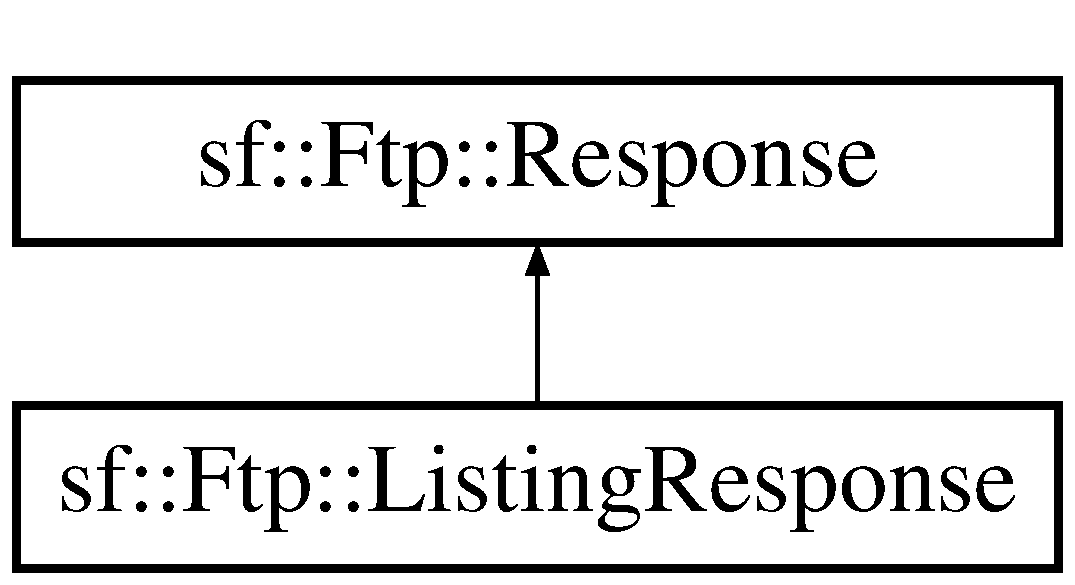
\includegraphics[height=2.000000cm]{classsf_1_1Ftp_1_1ListingResponse}
\end{center}
\end{figure}
\subsection*{Public Member Functions}
\begin{DoxyCompactItemize}
\item 
\hyperlink{classsf_1_1Ftp_1_1ListingResponse_aefc1b85e59ee0c3ee180666b4a4631e4}{Listing\-Response} (const \hyperlink{classsf_1_1Ftp_1_1Response}{Response} \&response, const std\-::vector$<$ char $>$ \&data)
\begin{DoxyCompactList}\small\item\em Default constructor. \end{DoxyCompactList}\item 
const std\-::vector$<$ std\-::string $>$ \& \hyperlink{classsf_1_1Ftp_1_1ListingResponse_a5f0771b52a966bf25b33a70602b6f97f}{get\-Listing} () const 
\begin{DoxyCompactList}\small\item\em Return the array of directory/file names. \end{DoxyCompactList}\end{DoxyCompactItemize}
\subsection*{Additional Inherited Members}


\subsection{Detailed Description}
Specialization of F\-T\-P response returning a filename lisiting. 

Definition at line 221 of file Ftp.\-hpp.



\subsection{Constructor \& Destructor Documentation}
\hypertarget{classsf_1_1Ftp_1_1ListingResponse_aefc1b85e59ee0c3ee180666b4a4631e4}{\index{sf\-::\-Ftp\-::\-Listing\-Response@{sf\-::\-Ftp\-::\-Listing\-Response}!Listing\-Response@{Listing\-Response}}
\index{Listing\-Response@{Listing\-Response}!sf::Ftp::ListingResponse@{sf\-::\-Ftp\-::\-Listing\-Response}}
\subsubsection[{Listing\-Response}]{\setlength{\rightskip}{0pt plus 5cm}sf\-::\-Ftp\-::\-Listing\-Response\-::\-Listing\-Response (
\begin{DoxyParamCaption}
\item[{const {\bf Response} \&}]{response, }
\item[{const std\-::vector$<$ char $>$ \&}]{data}
\end{DoxyParamCaption}
)}}\label{classsf_1_1Ftp_1_1ListingResponse_aefc1b85e59ee0c3ee180666b4a4631e4}


Default constructor. 


\begin{DoxyParams}{Parameters}
{\em response} & Source response \\
\hline
{\em data} & Data containing the raw listing \\
\hline
\end{DoxyParams}


\subsection{Member Function Documentation}
\hypertarget{classsf_1_1Ftp_1_1ListingResponse_a5f0771b52a966bf25b33a70602b6f97f}{\index{sf\-::\-Ftp\-::\-Listing\-Response@{sf\-::\-Ftp\-::\-Listing\-Response}!get\-Listing@{get\-Listing}}
\index{get\-Listing@{get\-Listing}!sf::Ftp::ListingResponse@{sf\-::\-Ftp\-::\-Listing\-Response}}
\subsubsection[{get\-Listing}]{\setlength{\rightskip}{0pt plus 5cm}const std\-::vector$<$std\-::string$>$\& sf\-::\-Ftp\-::\-Listing\-Response\-::get\-Listing (
\begin{DoxyParamCaption}
{}
\end{DoxyParamCaption}
) const}}\label{classsf_1_1Ftp_1_1ListingResponse_a5f0771b52a966bf25b33a70602b6f97f}


Return the array of directory/file names. 

\begin{DoxyReturn}{Returns}
Array containing the requested listing 
\end{DoxyReturn}


The documentation for this class was generated from the following file\-:\begin{DoxyCompactItemize}
\item 
/home/z\-Zelman/\-Dropbox/\-Placeholder-\/\-R\-T\-S/\-S\-F\-M\-L-\/2.\-1/include/\-S\-F\-M\-L/\-Network/Ftp.\-hpp\end{DoxyCompactItemize}

\hypertarget{classsf_1_1Lock}{\section{sf\-:\-:Lock Class Reference}
\label{classsf_1_1Lock}\index{sf\-::\-Lock@{sf\-::\-Lock}}
}


Automatic wrapper for locking and unlocking mutexes.  




{\ttfamily \#include $<$Lock.\-hpp$>$}

Inheritance diagram for sf\-:\-:Lock\-:\begin{figure}[H]
\begin{center}
\leavevmode
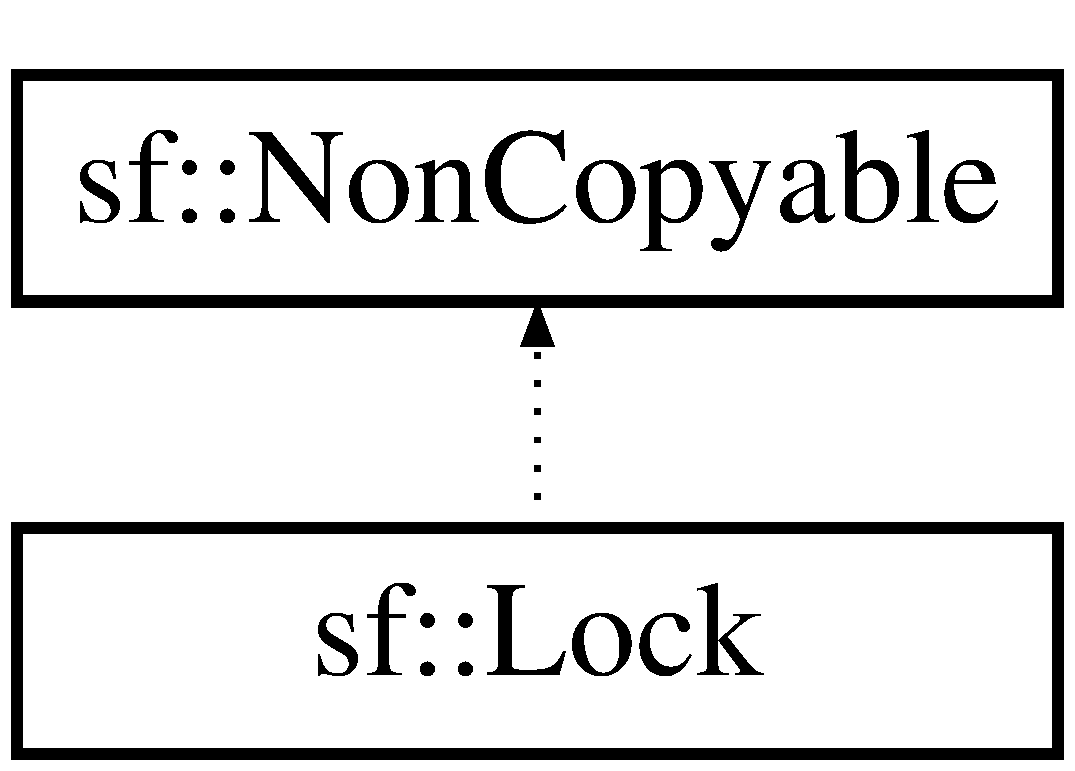
\includegraphics[height=2.000000cm]{classsf_1_1Lock}
\end{center}
\end{figure}
\subsection*{Public Member Functions}
\begin{DoxyCompactItemize}
\item 
\hyperlink{classsf_1_1Lock_a1a4c5d7a15da61103d85c9aa7f118920}{Lock} (\hyperlink{classsf_1_1Mutex}{Mutex} \&mutex)
\begin{DoxyCompactList}\small\item\em Construct the lock with a target mutex. \end{DoxyCompactList}\item 
\hyperlink{classsf_1_1Lock_a8168b36323a18ccf5b6bc531d964aec5}{$\sim$\-Lock} ()
\begin{DoxyCompactList}\small\item\em Destructor. \end{DoxyCompactList}\end{DoxyCompactItemize}


\subsection{Detailed Description}
Automatic wrapper for locking and unlocking mutexes. 

\hyperlink{classsf_1_1Lock}{sf\-::\-Lock} is a R\-A\-I\-I wrapper for \hyperlink{classsf_1_1Mutex}{sf\-::\-Mutex}. By unlocking it in its destructor, it ensures that the mutex will always be released when the current scope (most likely a function) ends. This is even more important when an exception or an early return statement can interrupt the execution flow of the function.

For maximum robustness, \hyperlink{classsf_1_1Lock}{sf\-::\-Lock} should always be used to lock/unlock a mutex.

Usage example\-: 
\begin{DoxyCode}
\hyperlink{classsf_1_1Mutex}{sf::Mutex} mutex;

\textcolor{keywordtype}{void} \textcolor{keyword}{function}()
\{
    \hyperlink{classsf_1_1Lock}{sf::Lock} lock(mutex); \textcolor{comment}{// mutex is now locked}

    functionThatMayThrowAnException(); \textcolor{comment}{// mutex is unlocked if this function throws}

    \textcolor{keywordflow}{if} (someCondition)
        \textcolor{keywordflow}{return}; \textcolor{comment}{// mutex is unlocked}

\} \textcolor{comment}{// mutex is unlocked}
\end{DoxyCode}


Because the mutex is not explicitely unlocked in the code, it may remain locked longer than needed. If the region of the code that needs to be protected by the mutex is not the entire function, a good practice is to create a smaller, inner scope so that the lock is limited to this part of the code.


\begin{DoxyCode}
\hyperlink{classsf_1_1Mutex}{sf::Mutex} mutex;

\textcolor{keywordtype}{void} \textcolor{keyword}{function}()
\{
    \{
      \hyperlink{classsf_1_1Lock}{sf::Lock} lock(mutex);
      codeThatRequiresProtection();

    \} \textcolor{comment}{// mutex is unlocked here}

    codeThatDoesntCareAboutTheMutex();
\}
\end{DoxyCode}


Having a mutex locked longer than required is a bad practice which can lead to bad performances. Don't forget that when a mutex is locked, other threads may be waiting doing nothing until it is released.

\begin{DoxySeeAlso}{See Also}
\hyperlink{classsf_1_1Mutex}{sf\-::\-Mutex} 
\end{DoxySeeAlso}


Definition at line 43 of file Lock.\-hpp.



\subsection{Constructor \& Destructor Documentation}
\hypertarget{classsf_1_1Lock_a1a4c5d7a15da61103d85c9aa7f118920}{\index{sf\-::\-Lock@{sf\-::\-Lock}!Lock@{Lock}}
\index{Lock@{Lock}!sf::Lock@{sf\-::\-Lock}}
\subsubsection[{Lock}]{\setlength{\rightskip}{0pt plus 5cm}sf\-::\-Lock\-::\-Lock (
\begin{DoxyParamCaption}
\item[{{\bf Mutex} \&}]{mutex}
\end{DoxyParamCaption}
)\hspace{0.3cm}{\ttfamily [explicit]}}}\label{classsf_1_1Lock_a1a4c5d7a15da61103d85c9aa7f118920}


Construct the lock with a target mutex. 

The mutex passed to \hyperlink{classsf_1_1Lock}{sf\-::\-Lock} is automatically locked.


\begin{DoxyParams}{Parameters}
{\em mutex} & \hyperlink{classsf_1_1Mutex}{Mutex} to lock \\
\hline
\end{DoxyParams}
\hypertarget{classsf_1_1Lock_a8168b36323a18ccf5b6bc531d964aec5}{\index{sf\-::\-Lock@{sf\-::\-Lock}!$\sim$\-Lock@{$\sim$\-Lock}}
\index{$\sim$\-Lock@{$\sim$\-Lock}!sf::Lock@{sf\-::\-Lock}}
\subsubsection[{$\sim$\-Lock}]{\setlength{\rightskip}{0pt plus 5cm}sf\-::\-Lock\-::$\sim$\-Lock (
\begin{DoxyParamCaption}
{}
\end{DoxyParamCaption}
)}}\label{classsf_1_1Lock_a8168b36323a18ccf5b6bc531d964aec5}


Destructor. 

The destructor of \hyperlink{classsf_1_1Lock}{sf\-::\-Lock} automatically unlocks its mutex. 

The documentation for this class was generated from the following file\-:\begin{DoxyCompactItemize}
\item 
/home/z\-Zelman/\-Dropbox/\-Placeholder-\/\-R\-T\-S/\-S\-F\-M\-L-\/2.\-1/include/\-S\-F\-M\-L/\-System/Lock.\-hpp\end{DoxyCompactItemize}

\hypertarget{classrapidxml_1_1memory__pool}{\section{rapidxml\-:\-:memory\-\_\-pool$<$ Ch $>$ Class Template Reference}
\label{classrapidxml_1_1memory__pool}\index{rapidxml\-::memory\-\_\-pool$<$ Ch $>$@{rapidxml\-::memory\-\_\-pool$<$ Ch $>$}}
}


{\ttfamily \#include $<$rapidxml.\-hpp$>$}

Inheritance diagram for rapidxml\-:\-:memory\-\_\-pool$<$ Ch $>$\-:\begin{figure}[H]
\begin{center}
\leavevmode
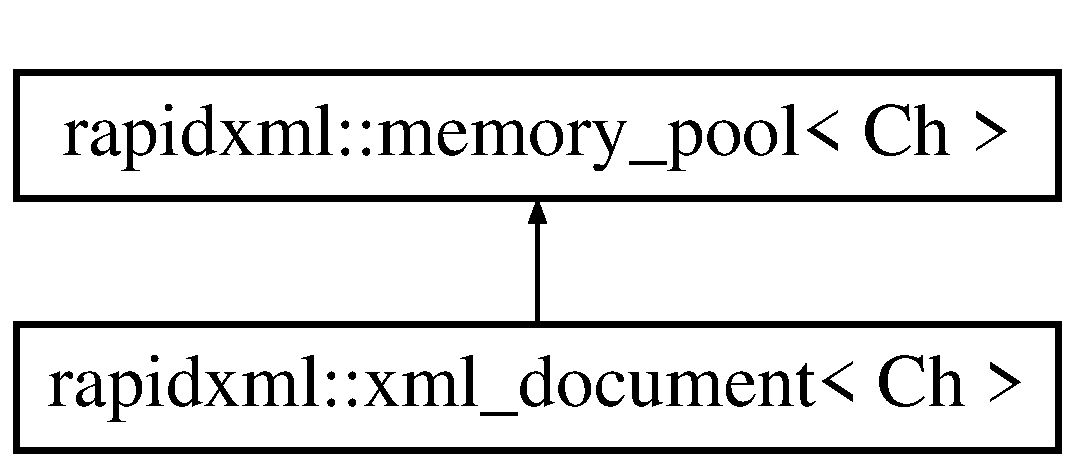
\includegraphics[height=2.000000cm]{classrapidxml_1_1memory__pool}
\end{center}
\end{figure}
\subsection*{Public Member Functions}
\begin{DoxyCompactItemize}
\item 
\hypertarget{classrapidxml_1_1memory__pool_a0b609da81dff28a19ebd704400788429}{\hyperlink{classrapidxml_1_1memory__pool_a0b609da81dff28a19ebd704400788429}{memory\-\_\-pool} ()}\label{classrapidxml_1_1memory__pool_a0b609da81dff28a19ebd704400788429}

\begin{DoxyCompactList}\small\item\em Constructs empty pool with default allocator functions. \end{DoxyCompactList}\item 
\hyperlink{classrapidxml_1_1memory__pool_a0a3e82126e59e4077f41e933130bb5a0}{$\sim$memory\-\_\-pool} ()
\item 
\hyperlink{classrapidxml_1_1xml__node}{xml\-\_\-node}$<$ Ch $>$ $\ast$ \hyperlink{classrapidxml_1_1memory__pool_a4118581c29ee9a2f6b55ebf7dac185f8}{allocate\-\_\-node} (node\-\_\-type type, const Ch $\ast$name=0, const Ch $\ast$value=0, std\-::size\-\_\-t name\-\_\-size=0, std\-::size\-\_\-t value\-\_\-size=0)
\item 
\hyperlink{classrapidxml_1_1xml__attribute}{xml\-\_\-attribute}$<$ Ch $>$ $\ast$ \hyperlink{classrapidxml_1_1memory__pool_a3de2a66c983336e006ea3844e244ed30}{allocate\-\_\-attribute} (const Ch $\ast$name=0, const Ch $\ast$value=0, std\-::size\-\_\-t name\-\_\-size=0, std\-::size\-\_\-t value\-\_\-size=0)
\item 
Ch $\ast$ \hyperlink{classrapidxml_1_1memory__pool_a171941b39d55b868358da97462185f58}{allocate\-\_\-string} (const Ch $\ast$source=0, std\-::size\-\_\-t size=0)
\item 
\hyperlink{classrapidxml_1_1xml__node}{xml\-\_\-node}$<$ Ch $>$ $\ast$ \hyperlink{classrapidxml_1_1memory__pool_a0a10679fc17597d339a0dc107f8a94ac}{clone\-\_\-node} (const \hyperlink{classrapidxml_1_1xml__node}{xml\-\_\-node}$<$ Ch $>$ $\ast$source, \hyperlink{classrapidxml_1_1xml__node}{xml\-\_\-node}$<$ Ch $>$ $\ast$result=0)
\item 
void \hyperlink{classrapidxml_1_1memory__pool_aad377c835fdaed1cb2cc9df194cf84e4}{clear} ()
\item 
void \hyperlink{classrapidxml_1_1memory__pool_a84d3d8d2cdfc00501e1dcf26d889ae03}{set\-\_\-allocator} (alloc\-\_\-func $\ast$af, free\-\_\-func $\ast$ff)
\end{DoxyCompactItemize}


\subsection{Detailed Description}
\subsubsection*{template$<$class Ch = char$>$class rapidxml\-::memory\-\_\-pool$<$ Ch $>$}

This class is used by the parser to create new nodes and attributes, without overheads of dynamic memory allocation. In most cases, you will not need to use this class directly. However, if you need to create nodes manually or modify names/values of nodes, you are encouraged to use \hyperlink{classrapidxml_1_1memory__pool}{memory\-\_\-pool} of relevant \hyperlink{classrapidxml_1_1xml__document}{xml\-\_\-document} to allocate the memory. Not only is this faster than allocating them by using {\ttfamily new} operator, but also their lifetime will be tied to the lifetime of document, possibly simplyfing memory management. \par
\par
 Call \hyperlink{classrapidxml_1_1memory__pool_a4118581c29ee9a2f6b55ebf7dac185f8}{allocate\-\_\-node()} or \hyperlink{classrapidxml_1_1memory__pool_a3de2a66c983336e006ea3844e244ed30}{allocate\-\_\-attribute()} functions to obtain new nodes or attributes from the pool. You can also call \hyperlink{classrapidxml_1_1memory__pool_a171941b39d55b868358da97462185f58}{allocate\-\_\-string()} function to allocate strings. Such strings can then be used as names or values of nodes without worrying about their lifetime. Note that there is no {\ttfamily free()} function -- all allocations are freed at once when \hyperlink{classrapidxml_1_1memory__pool_aad377c835fdaed1cb2cc9df194cf84e4}{clear()} function is called, or when the pool is destroyed. \par
\par
 It is also possible to create a standalone \hyperlink{classrapidxml_1_1memory__pool}{memory\-\_\-pool}, and use it to allocate nodes, whose lifetime will not be tied to any document. \par
\par
 Pool maintains {\ttfamily R\-A\-P\-I\-D\-X\-M\-L\-\_\-\-S\-T\-A\-T\-I\-C\-\_\-\-P\-O\-O\-L\-\_\-\-S\-I\-Z\-E} bytes of statically allocated memory. Until static memory is exhausted, no dynamic memory allocations are done. When static memory is exhausted, pool allocates additional blocks of memory of size {\ttfamily R\-A\-P\-I\-D\-X\-M\-L\-\_\-\-D\-Y\-N\-A\-M\-I\-C\-\_\-\-P\-O\-O\-L\-\_\-\-S\-I\-Z\-E} each, by using global {\ttfamily new\mbox{[}\mbox{]}} and {\ttfamily delete\mbox{[}\mbox{]}} operators. This behaviour can be changed by setting custom allocation routines. Use \hyperlink{classrapidxml_1_1memory__pool_a84d3d8d2cdfc00501e1dcf26d889ae03}{set\-\_\-allocator()} function to set them. \par
\par
 Allocations for nodes, attributes and strings are aligned at {\ttfamily R\-A\-P\-I\-D\-X\-M\-L\-\_\-\-A\-L\-I\-G\-N\-M\-E\-N\-T} bytes. This value defaults to the size of pointer on target architecture. \par
\par
 To obtain absolutely top performance from the parser, it is important that all nodes are allocated from a single, contiguous block of memory. Otherwise, cache misses when jumping between two (or more) disjoint blocks of memory can slow down parsing quite considerably. If required, you can tweak {\ttfamily R\-A\-P\-I\-D\-X\-M\-L\-\_\-\-S\-T\-A\-T\-I\-C\-\_\-\-P\-O\-O\-L\-\_\-\-S\-I\-Z\-E}, {\ttfamily R\-A\-P\-I\-D\-X\-M\-L\-\_\-\-D\-Y\-N\-A\-M\-I\-C\-\_\-\-P\-O\-O\-L\-\_\-\-S\-I\-Z\-E} and {\ttfamily R\-A\-P\-I\-D\-X\-M\-L\-\_\-\-A\-L\-I\-G\-N\-M\-E\-N\-T} to obtain best wasted memory to performance compromise. To do it, define their values before \hyperlink{rapidxml_8hpp}{rapidxml.\-hpp} file is included. 
\begin{DoxyParams}{Parameters}
{\em Ch} & Character type of created nodes. \\
\hline
\end{DoxyParams}


Definition at line 379 of file rapidxml.\-hpp.



\subsection{Constructor \& Destructor Documentation}
\hypertarget{classrapidxml_1_1memory__pool_a0a3e82126e59e4077f41e933130bb5a0}{\index{rapidxml\-::memory\-\_\-pool@{rapidxml\-::memory\-\_\-pool}!$\sim$memory\-\_\-pool@{$\sim$memory\-\_\-pool}}
\index{$\sim$memory\-\_\-pool@{$\sim$memory\-\_\-pool}!rapidxml::memory_pool@{rapidxml\-::memory\-\_\-pool}}
\subsubsection[{$\sim$memory\-\_\-pool}]{\setlength{\rightskip}{0pt plus 5cm}template$<$class Ch  = char$>$ {\bf rapidxml\-::memory\-\_\-pool}$<$ Ch $>$\-::$\sim${\bf memory\-\_\-pool} (
\begin{DoxyParamCaption}
{}
\end{DoxyParamCaption}
)\hspace{0.3cm}{\ttfamily [inline]}}}\label{classrapidxml_1_1memory__pool_a0a3e82126e59e4077f41e933130bb5a0}
Destroys pool and frees all the memory. This causes memory occupied by nodes allocated by the pool to be freed. Nodes allocated from the pool are no longer valid. 

Definition at line 400 of file rapidxml.\-hpp.



\subsection{Member Function Documentation}
\hypertarget{classrapidxml_1_1memory__pool_a3de2a66c983336e006ea3844e244ed30}{\index{rapidxml\-::memory\-\_\-pool@{rapidxml\-::memory\-\_\-pool}!allocate\-\_\-attribute@{allocate\-\_\-attribute}}
\index{allocate\-\_\-attribute@{allocate\-\_\-attribute}!rapidxml::memory_pool@{rapidxml\-::memory\-\_\-pool}}
\subsubsection[{allocate\-\_\-attribute}]{\setlength{\rightskip}{0pt plus 5cm}template$<$class Ch  = char$>$ {\bf xml\-\_\-attribute}$<$Ch$>$$\ast$ {\bf rapidxml\-::memory\-\_\-pool}$<$ Ch $>$\-::allocate\-\_\-attribute (
\begin{DoxyParamCaption}
\item[{const Ch $\ast$}]{name = {\ttfamily 0}, }
\item[{const Ch $\ast$}]{value = {\ttfamily 0}, }
\item[{std\-::size\-\_\-t}]{name\-\_\-size = {\ttfamily 0}, }
\item[{std\-::size\-\_\-t}]{value\-\_\-size = {\ttfamily 0}}
\end{DoxyParamCaption}
)\hspace{0.3cm}{\ttfamily [inline]}}}\label{classrapidxml_1_1memory__pool_a3de2a66c983336e006ea3844e244ed30}
Allocates a new attribute from the pool, and optionally assigns name and value to it. If the allocation request cannot be accomodated, this function will throw {\ttfamily std\-::bad\-\_\-alloc}. If exceptions are disabled by defining R\-A\-P\-I\-D\-X\-M\-L\-\_\-\-N\-O\-\_\-\-E\-X\-C\-E\-P\-T\-I\-O\-N\-S, this function will call rapidxml\-::parse\-\_\-error\-\_\-handler() function. 
\begin{DoxyParams}{Parameters}
{\em name} & Name to assign to the attribute, or 0 to assign no name. \\
\hline
{\em value} & Value to assign to the attribute, or 0 to assign no value. \\
\hline
{\em name\-\_\-size} & Size of name to assign, or 0 to automatically calculate size from name string. \\
\hline
{\em value\-\_\-size} & Size of value to assign, or 0 to automatically calculate size from value string. \\
\hline
\end{DoxyParams}
\begin{DoxyReturn}{Returns}
Pointer to allocated attribute. This pointer will never be N\-U\-L\-L. 
\end{DoxyReturn}


Definition at line 447 of file rapidxml.\-hpp.

\hypertarget{classrapidxml_1_1memory__pool_a4118581c29ee9a2f6b55ebf7dac185f8}{\index{rapidxml\-::memory\-\_\-pool@{rapidxml\-::memory\-\_\-pool}!allocate\-\_\-node@{allocate\-\_\-node}}
\index{allocate\-\_\-node@{allocate\-\_\-node}!rapidxml::memory_pool@{rapidxml\-::memory\-\_\-pool}}
\subsubsection[{allocate\-\_\-node}]{\setlength{\rightskip}{0pt plus 5cm}template$<$class Ch  = char$>$ {\bf xml\-\_\-node}$<$Ch$>$$\ast$ {\bf rapidxml\-::memory\-\_\-pool}$<$ Ch $>$\-::allocate\-\_\-node (
\begin{DoxyParamCaption}
\item[{node\-\_\-type}]{type, }
\item[{const Ch $\ast$}]{name = {\ttfamily 0}, }
\item[{const Ch $\ast$}]{value = {\ttfamily 0}, }
\item[{std\-::size\-\_\-t}]{name\-\_\-size = {\ttfamily 0}, }
\item[{std\-::size\-\_\-t}]{value\-\_\-size = {\ttfamily 0}}
\end{DoxyParamCaption}
)\hspace{0.3cm}{\ttfamily [inline]}}}\label{classrapidxml_1_1memory__pool_a4118581c29ee9a2f6b55ebf7dac185f8}
Allocates a new node from the pool, and optionally assigns name and value to it. If the allocation request cannot be accomodated, this function will throw {\ttfamily std\-::bad\-\_\-alloc}. If exceptions are disabled by defining R\-A\-P\-I\-D\-X\-M\-L\-\_\-\-N\-O\-\_\-\-E\-X\-C\-E\-P\-T\-I\-O\-N\-S, this function will call rapidxml\-::parse\-\_\-error\-\_\-handler() function. 
\begin{DoxyParams}{Parameters}
{\em type} & Type of node to create. \\
\hline
{\em name} & Name to assign to the node, or 0 to assign no name. \\
\hline
{\em value} & Value to assign to the node, or 0 to assign no value. \\
\hline
{\em name\-\_\-size} & Size of name to assign, or 0 to automatically calculate size from name string. \\
\hline
{\em value\-\_\-size} & Size of value to assign, or 0 to automatically calculate size from value string. \\
\hline
\end{DoxyParams}
\begin{DoxyReturn}{Returns}
Pointer to allocated node. This pointer will never be N\-U\-L\-L. 
\end{DoxyReturn}


Definition at line 415 of file rapidxml.\-hpp.

\hypertarget{classrapidxml_1_1memory__pool_a171941b39d55b868358da97462185f58}{\index{rapidxml\-::memory\-\_\-pool@{rapidxml\-::memory\-\_\-pool}!allocate\-\_\-string@{allocate\-\_\-string}}
\index{allocate\-\_\-string@{allocate\-\_\-string}!rapidxml::memory_pool@{rapidxml\-::memory\-\_\-pool}}
\subsubsection[{allocate\-\_\-string}]{\setlength{\rightskip}{0pt plus 5cm}template$<$class Ch  = char$>$ Ch$\ast$ {\bf rapidxml\-::memory\-\_\-pool}$<$ Ch $>$\-::allocate\-\_\-string (
\begin{DoxyParamCaption}
\item[{const Ch $\ast$}]{source = {\ttfamily 0}, }
\item[{std\-::size\-\_\-t}]{size = {\ttfamily 0}}
\end{DoxyParamCaption}
)\hspace{0.3cm}{\ttfamily [inline]}}}\label{classrapidxml_1_1memory__pool_a171941b39d55b868358da97462185f58}
Allocates a char array of given size from the pool, and optionally copies a given string to it. If the allocation request cannot be accomodated, this function will throw {\ttfamily std\-::bad\-\_\-alloc}. If exceptions are disabled by defining R\-A\-P\-I\-D\-X\-M\-L\-\_\-\-N\-O\-\_\-\-E\-X\-C\-E\-P\-T\-I\-O\-N\-S, this function will call rapidxml\-::parse\-\_\-error\-\_\-handler() function. 
\begin{DoxyParams}{Parameters}
{\em source} & String to initialize the allocated memory with, or 0 to not initialize it. \\
\hline
{\em size} & Number of characters to allocate, or zero to calculate it automatically from source string length; if size is 0, source string must be specified and null terminated. \\
\hline
\end{DoxyParams}
\begin{DoxyReturn}{Returns}
Pointer to allocated char array. This pointer will never be N\-U\-L\-L. 
\end{DoxyReturn}


Definition at line 476 of file rapidxml.\-hpp.

\hypertarget{classrapidxml_1_1memory__pool_aad377c835fdaed1cb2cc9df194cf84e4}{\index{rapidxml\-::memory\-\_\-pool@{rapidxml\-::memory\-\_\-pool}!clear@{clear}}
\index{clear@{clear}!rapidxml::memory_pool@{rapidxml\-::memory\-\_\-pool}}
\subsubsection[{clear}]{\setlength{\rightskip}{0pt plus 5cm}template$<$class Ch  = char$>$ void {\bf rapidxml\-::memory\-\_\-pool}$<$ Ch $>$\-::clear (
\begin{DoxyParamCaption}
{}
\end{DoxyParamCaption}
)\hspace{0.3cm}{\ttfamily [inline]}}}\label{classrapidxml_1_1memory__pool_aad377c835fdaed1cb2cc9df194cf84e4}
Clears the pool. This causes memory occupied by nodes allocated by the pool to be freed. Any nodes or strings allocated from the pool will no longer be valid. 

Definition at line 525 of file rapidxml.\-hpp.

\hypertarget{classrapidxml_1_1memory__pool_a0a10679fc17597d339a0dc107f8a94ac}{\index{rapidxml\-::memory\-\_\-pool@{rapidxml\-::memory\-\_\-pool}!clone\-\_\-node@{clone\-\_\-node}}
\index{clone\-\_\-node@{clone\-\_\-node}!rapidxml::memory_pool@{rapidxml\-::memory\-\_\-pool}}
\subsubsection[{clone\-\_\-node}]{\setlength{\rightskip}{0pt plus 5cm}template$<$class Ch  = char$>$ {\bf xml\-\_\-node}$<$Ch$>$$\ast$ {\bf rapidxml\-::memory\-\_\-pool}$<$ Ch $>$\-::clone\-\_\-node (
\begin{DoxyParamCaption}
\item[{const {\bf xml\-\_\-node}$<$ Ch $>$ $\ast$}]{source, }
\item[{{\bf xml\-\_\-node}$<$ Ch $>$ $\ast$}]{result = {\ttfamily 0}}
\end{DoxyParamCaption}
)\hspace{0.3cm}{\ttfamily [inline]}}}\label{classrapidxml_1_1memory__pool_a0a10679fc17597d339a0dc107f8a94ac}
Clones an \hyperlink{classrapidxml_1_1xml__node}{xml\-\_\-node} and its hierarchy of child nodes and attributes. Nodes and attributes are allocated from this memory pool. Names and values are not cloned, they are shared between the clone and the source. Result node can be optionally specified as a second parameter, in which case its contents will be replaced with cloned source node. This is useful when you want to clone entire document. 
\begin{DoxyParams}{Parameters}
{\em source} & Node to clone. \\
\hline
{\em result} & Node to put results in, or 0 to automatically allocate result node \\
\hline
\end{DoxyParams}
\begin{DoxyReturn}{Returns}
Pointer to cloned node. This pointer will never be N\-U\-L\-L. 
\end{DoxyReturn}


Definition at line 497 of file rapidxml.\-hpp.

\hypertarget{classrapidxml_1_1memory__pool_a84d3d8d2cdfc00501e1dcf26d889ae03}{\index{rapidxml\-::memory\-\_\-pool@{rapidxml\-::memory\-\_\-pool}!set\-\_\-allocator@{set\-\_\-allocator}}
\index{set\-\_\-allocator@{set\-\_\-allocator}!rapidxml::memory_pool@{rapidxml\-::memory\-\_\-pool}}
\subsubsection[{set\-\_\-allocator}]{\setlength{\rightskip}{0pt plus 5cm}template$<$class Ch  = char$>$ void {\bf rapidxml\-::memory\-\_\-pool}$<$ Ch $>$\-::set\-\_\-allocator (
\begin{DoxyParamCaption}
\item[{alloc\-\_\-func $\ast$}]{af, }
\item[{free\-\_\-func $\ast$}]{ff}
\end{DoxyParamCaption}
)\hspace{0.3cm}{\ttfamily [inline]}}}\label{classrapidxml_1_1memory__pool_a84d3d8d2cdfc00501e1dcf26d889ae03}
Sets or resets the user-\/defined memory allocation functions for the pool. This can only be called when no memory is allocated from the pool yet, otherwise results are undefined. Allocation function must not return invalid pointer on failure. It should either throw, stop the program, or use {\ttfamily longjmp()} function to pass control to other place of program. If it returns invalid pointer, results are undefined. \par
\par
 User defined allocation functions must have the following forms\-: \par
{\ttfamily  \par
void $\ast$allocate(std\-::size\-\_\-t size); \par
void free(void $\ast$pointer); }\par
 
\begin{DoxyParams}{Parameters}
{\em af} & Allocation function, or 0 to restore default function \\
\hline
{\em ff} & Free function, or 0 to restore default function \\
\hline
\end{DoxyParams}


Definition at line 552 of file rapidxml.\-hpp.



The documentation for this class was generated from the following file\-:\begin{DoxyCompactItemize}
\item 
/home/z\-Zelman/\-Dropbox/\-Placeholder-\/\-R\-T\-S/rapidxml-\/1.\-13/\hyperlink{rapidxml_8hpp}{rapidxml.\-hpp}\end{DoxyCompactItemize}

\hypertarget{classsf_1_1Mouse}{\section{sf\-:\-:Mouse Class Reference}
\label{classsf_1_1Mouse}\index{sf\-::\-Mouse@{sf\-::\-Mouse}}
}


Give access to the real-\/time state of the mouse.  




{\ttfamily \#include $<$Mouse.\-hpp$>$}

\subsection*{Public Types}
\begin{DoxyCompactItemize}
\item 
enum \hyperlink{classsf_1_1Mouse_a4fb128be433f9aafe66bc0c605daaa90}{Button} \{ \\*
\hyperlink{classsf_1_1Mouse_a4fb128be433f9aafe66bc0c605daaa90a8bb4856e1ec7f6b6a8605effdfc0eee8}{Left}, 
\hyperlink{classsf_1_1Mouse_a4fb128be433f9aafe66bc0c605daaa90af2cff24ab6c26daf079b11189f982fc4}{Right}, 
\hyperlink{classsf_1_1Mouse_a4fb128be433f9aafe66bc0c605daaa90a2c353189c4b11cf216d7caddafcc609d}{Middle}, 
\hyperlink{classsf_1_1Mouse_a4fb128be433f9aafe66bc0c605daaa90aecc7f3ce9ad6a60b9b0027876446b8d7}{X\-Button1}, 
\\*
\hyperlink{classsf_1_1Mouse_a4fb128be433f9aafe66bc0c605daaa90a03fa056fd0dd9d629c205d91a8ef1b5a}{X\-Button2}, 
\hyperlink{classsf_1_1Mouse_a4fb128be433f9aafe66bc0c605daaa90a52a1d434289774240ddaa22496762402}{Button\-Count}
 \}
\begin{DoxyCompactList}\small\item\em \hyperlink{classsf_1_1Mouse}{Mouse} buttons. \end{DoxyCompactList}\end{DoxyCompactItemize}
\subsection*{Static Public Member Functions}
\begin{DoxyCompactItemize}
\item 
static bool \hyperlink{classsf_1_1Mouse_ab647159eb88e369a0332a9c5a7ba6687}{is\-Button\-Pressed} (\hyperlink{classsf_1_1Mouse_a4fb128be433f9aafe66bc0c605daaa90}{Button} button)
\begin{DoxyCompactList}\small\item\em Check if a mouse button is pressed. \end{DoxyCompactList}\item 
static \hyperlink{classsf_1_1Vector2}{Vector2i} \hyperlink{classsf_1_1Mouse_ac368680f797b7f6e4f50b5b7928c1387}{get\-Position} ()
\begin{DoxyCompactList}\small\item\em Get the current position of the mouse in desktop coordinates. \end{DoxyCompactList}\item 
static \hyperlink{classsf_1_1Vector2}{Vector2i} \hyperlink{classsf_1_1Mouse_a93b4d2ebef728e77a0ec9d83c1e0b0c8}{get\-Position} (const \hyperlink{classsf_1_1Window}{Window} \&relative\-To)
\begin{DoxyCompactList}\small\item\em Get the current position of the mouse in window coordinates. \end{DoxyCompactList}\item 
static void \hyperlink{classsf_1_1Mouse_a1222e16c583be9e3d176d86e0b7817d7}{set\-Position} (const \hyperlink{classsf_1_1Vector2}{Vector2i} \&position)
\begin{DoxyCompactList}\small\item\em Set the current position of the mouse in desktop coordinates. \end{DoxyCompactList}\item 
static void \hyperlink{classsf_1_1Mouse_ad9b16ec7041531315f06b26b413dfea8}{set\-Position} (const \hyperlink{classsf_1_1Vector2}{Vector2i} \&position, const \hyperlink{classsf_1_1Window}{Window} \&relative\-To)
\begin{DoxyCompactList}\small\item\em Set the current position of the mouse in window coordinates. \end{DoxyCompactList}\end{DoxyCompactItemize}


\subsection{Detailed Description}
Give access to the real-\/time state of the mouse. 

\hyperlink{classsf_1_1Mouse}{sf\-::\-Mouse} provides an interface to the state of the mouse. It only contains static functions (a single mouse is assumed), so it's not meant to be instanciated.

This class allows users to query the mouse state at any time and directly, without having to deal with a window and its events. Compared to the Mouse\-Moved, Mouse\-Button\-Pressed and Mouse\-Button\-Released events, \hyperlink{classsf_1_1Mouse}{sf\-::\-Mouse} can retrieve the state of the cursor and the buttons at any time (you don't need to store and update a boolean on your side in order to know if a button is pressed or released), and you always get the real state of the mouse, even if it is moved, pressed or released when your window is out of focus and no event is triggered.

The set\-Position and get\-Position functions can be used to change or retrieve the current position of the mouse pointer. There are two versions\-: one that operates in global coordinates (relative to the desktop) and one that operates in window coordinates (relative to a specific window).

Usage example\-: 
\begin{DoxyCode}
\textcolor{keywordflow}{if} (\hyperlink{classsf_1_1Mouse_ab647159eb88e369a0332a9c5a7ba6687}{sf::Mouse::isButtonPressed}(\hyperlink{classsf_1_1Mouse_a4fb128be433f9aafe66bc0c605daaa90a8bb4856e1ec7f6b6a8605effdfc0eee8}{sf::Mouse::Left}))
\{
    \textcolor{comment}{// left click...}
\}

\textcolor{comment}{// get global mouse position}
\hyperlink{classsf_1_1Vector2}{sf::Vector2i} position = \hyperlink{classsf_1_1Mouse_ac368680f797b7f6e4f50b5b7928c1387}{sf::Mouse::getPosition}();

\textcolor{comment}{// set mouse position relative to a window}
\hyperlink{classsf_1_1Mouse_a1222e16c583be9e3d176d86e0b7817d7}{sf::Mouse::setPosition}(\hyperlink{classsf_1_1Vector2}{sf::Vector2i}(100, 200), window);
\end{DoxyCode}


\begin{DoxySeeAlso}{See Also}
\hyperlink{classsf_1_1Joystick}{sf\-::\-Joystick}, \hyperlink{classsf_1_1Keyboard}{sf\-::\-Keyboard} 
\end{DoxySeeAlso}


Definition at line 43 of file Mouse.\-hpp.



\subsection{Member Enumeration Documentation}
\hypertarget{classsf_1_1Mouse_a4fb128be433f9aafe66bc0c605daaa90}{\index{sf\-::\-Mouse@{sf\-::\-Mouse}!Button@{Button}}
\index{Button@{Button}!sf::Mouse@{sf\-::\-Mouse}}
\subsubsection[{Button}]{\setlength{\rightskip}{0pt plus 5cm}enum {\bf sf\-::\-Mouse\-::\-Button}}}\label{classsf_1_1Mouse_a4fb128be433f9aafe66bc0c605daaa90}


\hyperlink{classsf_1_1Mouse}{Mouse} buttons. 

\begin{Desc}
\item[Enumerator]\par
\begin{description}
\index{Left@{Left}!sf\-::\-Mouse@{sf\-::\-Mouse}}\index{sf\-::\-Mouse@{sf\-::\-Mouse}!Left@{Left}}\item[{\em 
\hypertarget{classsf_1_1Mouse_a4fb128be433f9aafe66bc0c605daaa90a8bb4856e1ec7f6b6a8605effdfc0eee8}{Left}\label{classsf_1_1Mouse_a4fb128be433f9aafe66bc0c605daaa90a8bb4856e1ec7f6b6a8605effdfc0eee8}
}]The left mouse button. \index{Right@{Right}!sf\-::\-Mouse@{sf\-::\-Mouse}}\index{sf\-::\-Mouse@{sf\-::\-Mouse}!Right@{Right}}\item[{\em 
\hypertarget{classsf_1_1Mouse_a4fb128be433f9aafe66bc0c605daaa90af2cff24ab6c26daf079b11189f982fc4}{Right}\label{classsf_1_1Mouse_a4fb128be433f9aafe66bc0c605daaa90af2cff24ab6c26daf079b11189f982fc4}
}]The right mouse button. \index{Middle@{Middle}!sf\-::\-Mouse@{sf\-::\-Mouse}}\index{sf\-::\-Mouse@{sf\-::\-Mouse}!Middle@{Middle}}\item[{\em 
\hypertarget{classsf_1_1Mouse_a4fb128be433f9aafe66bc0c605daaa90a2c353189c4b11cf216d7caddafcc609d}{Middle}\label{classsf_1_1Mouse_a4fb128be433f9aafe66bc0c605daaa90a2c353189c4b11cf216d7caddafcc609d}
}]The middle (wheel) mouse button. \index{X\-Button1@{X\-Button1}!sf\-::\-Mouse@{sf\-::\-Mouse}}\index{sf\-::\-Mouse@{sf\-::\-Mouse}!X\-Button1@{X\-Button1}}\item[{\em 
\hypertarget{classsf_1_1Mouse_a4fb128be433f9aafe66bc0c605daaa90aecc7f3ce9ad6a60b9b0027876446b8d7}{X\-Button1}\label{classsf_1_1Mouse_a4fb128be433f9aafe66bc0c605daaa90aecc7f3ce9ad6a60b9b0027876446b8d7}
}]The first extra mouse button. \index{X\-Button2@{X\-Button2}!sf\-::\-Mouse@{sf\-::\-Mouse}}\index{sf\-::\-Mouse@{sf\-::\-Mouse}!X\-Button2@{X\-Button2}}\item[{\em 
\hypertarget{classsf_1_1Mouse_a4fb128be433f9aafe66bc0c605daaa90a03fa056fd0dd9d629c205d91a8ef1b5a}{X\-Button2}\label{classsf_1_1Mouse_a4fb128be433f9aafe66bc0c605daaa90a03fa056fd0dd9d629c205d91a8ef1b5a}
}]The second extra mouse button. \index{Button\-Count@{Button\-Count}!sf\-::\-Mouse@{sf\-::\-Mouse}}\index{sf\-::\-Mouse@{sf\-::\-Mouse}!Button\-Count@{Button\-Count}}\item[{\em 
\hypertarget{classsf_1_1Mouse_a4fb128be433f9aafe66bc0c605daaa90a52a1d434289774240ddaa22496762402}{Button\-Count}\label{classsf_1_1Mouse_a4fb128be433f9aafe66bc0c605daaa90a52a1d434289774240ddaa22496762402}
}]Keep last -- the total number of mouse buttons. \end{description}
\end{Desc}


Definition at line 51 of file Mouse.\-hpp.



\subsection{Member Function Documentation}
\hypertarget{classsf_1_1Mouse_ac368680f797b7f6e4f50b5b7928c1387}{\index{sf\-::\-Mouse@{sf\-::\-Mouse}!get\-Position@{get\-Position}}
\index{get\-Position@{get\-Position}!sf::Mouse@{sf\-::\-Mouse}}
\subsubsection[{get\-Position}]{\setlength{\rightskip}{0pt plus 5cm}static {\bf Vector2i} sf\-::\-Mouse\-::get\-Position (
\begin{DoxyParamCaption}
{}
\end{DoxyParamCaption}
)\hspace{0.3cm}{\ttfamily [static]}}}\label{classsf_1_1Mouse_ac368680f797b7f6e4f50b5b7928c1387}


Get the current position of the mouse in desktop coordinates. 

This function returns the global position of the mouse cursor on the desktop.

\begin{DoxyReturn}{Returns}
Current position of the mouse 
\end{DoxyReturn}
\hypertarget{classsf_1_1Mouse_a93b4d2ebef728e77a0ec9d83c1e0b0c8}{\index{sf\-::\-Mouse@{sf\-::\-Mouse}!get\-Position@{get\-Position}}
\index{get\-Position@{get\-Position}!sf::Mouse@{sf\-::\-Mouse}}
\subsubsection[{get\-Position}]{\setlength{\rightskip}{0pt plus 5cm}static {\bf Vector2i} sf\-::\-Mouse\-::get\-Position (
\begin{DoxyParamCaption}
\item[{const {\bf Window} \&}]{relative\-To}
\end{DoxyParamCaption}
)\hspace{0.3cm}{\ttfamily [static]}}}\label{classsf_1_1Mouse_a93b4d2ebef728e77a0ec9d83c1e0b0c8}


Get the current position of the mouse in window coordinates. 

This function returns the current position of the mouse cursor, relative to the given window.


\begin{DoxyParams}{Parameters}
{\em relative\-To} & Reference window\\
\hline
\end{DoxyParams}
\begin{DoxyReturn}{Returns}
Current position of the mouse 
\end{DoxyReturn}
\hypertarget{classsf_1_1Mouse_ab647159eb88e369a0332a9c5a7ba6687}{\index{sf\-::\-Mouse@{sf\-::\-Mouse}!is\-Button\-Pressed@{is\-Button\-Pressed}}
\index{is\-Button\-Pressed@{is\-Button\-Pressed}!sf::Mouse@{sf\-::\-Mouse}}
\subsubsection[{is\-Button\-Pressed}]{\setlength{\rightskip}{0pt plus 5cm}static bool sf\-::\-Mouse\-::is\-Button\-Pressed (
\begin{DoxyParamCaption}
\item[{{\bf Button}}]{button}
\end{DoxyParamCaption}
)\hspace{0.3cm}{\ttfamily [static]}}}\label{classsf_1_1Mouse_ab647159eb88e369a0332a9c5a7ba6687}


Check if a mouse button is pressed. 


\begin{DoxyParams}{Parameters}
{\em button} & Button to check\\
\hline
\end{DoxyParams}
\begin{DoxyReturn}{Returns}
True if the button is pressed, false otherwise 
\end{DoxyReturn}
\hypertarget{classsf_1_1Mouse_a1222e16c583be9e3d176d86e0b7817d7}{\index{sf\-::\-Mouse@{sf\-::\-Mouse}!set\-Position@{set\-Position}}
\index{set\-Position@{set\-Position}!sf::Mouse@{sf\-::\-Mouse}}
\subsubsection[{set\-Position}]{\setlength{\rightskip}{0pt plus 5cm}static void sf\-::\-Mouse\-::set\-Position (
\begin{DoxyParamCaption}
\item[{const {\bf Vector2i} \&}]{position}
\end{DoxyParamCaption}
)\hspace{0.3cm}{\ttfamily [static]}}}\label{classsf_1_1Mouse_a1222e16c583be9e3d176d86e0b7817d7}


Set the current position of the mouse in desktop coordinates. 

This function sets the global position of the mouse cursor on the desktop.


\begin{DoxyParams}{Parameters}
{\em position} & New position of the mouse \\
\hline
\end{DoxyParams}
\hypertarget{classsf_1_1Mouse_ad9b16ec7041531315f06b26b413dfea8}{\index{sf\-::\-Mouse@{sf\-::\-Mouse}!set\-Position@{set\-Position}}
\index{set\-Position@{set\-Position}!sf::Mouse@{sf\-::\-Mouse}}
\subsubsection[{set\-Position}]{\setlength{\rightskip}{0pt plus 5cm}static void sf\-::\-Mouse\-::set\-Position (
\begin{DoxyParamCaption}
\item[{const {\bf Vector2i} \&}]{position, }
\item[{const {\bf Window} \&}]{relative\-To}
\end{DoxyParamCaption}
)\hspace{0.3cm}{\ttfamily [static]}}}\label{classsf_1_1Mouse_ad9b16ec7041531315f06b26b413dfea8}


Set the current position of the mouse in window coordinates. 

This function sets the current position of the mouse cursor, relative to the given window.


\begin{DoxyParams}{Parameters}
{\em position} & New position of the mouse \\
\hline
{\em relative\-To} & Reference window \\
\hline
\end{DoxyParams}


The documentation for this class was generated from the following file\-:\begin{DoxyCompactItemize}
\item 
/home/z\-Zelman/\-Dropbox/\-Placeholder-\/\-R\-T\-S/\-S\-F\-M\-L-\/2.\-1/include/\-S\-F\-M\-L/\-Window/Mouse.\-hpp\end{DoxyCompactItemize}

\hypertarget{structsf_1_1Event_1_1MouseButtonEvent}{\section{sf\-:\-:Event\-:\-:Mouse\-Button\-Event Struct Reference}
\label{structsf_1_1Event_1_1MouseButtonEvent}\index{sf\-::\-Event\-::\-Mouse\-Button\-Event@{sf\-::\-Event\-::\-Mouse\-Button\-Event}}
}


\hyperlink{classsf_1_1Mouse}{Mouse} buttons events parameters (Mouse\-Button\-Pressed, Mouse\-Button\-Released)  




{\ttfamily \#include $<$Event.\-hpp$>$}

\subsection*{Public Attributes}
\begin{DoxyCompactItemize}
\item 
\hypertarget{structsf_1_1Event_1_1MouseButtonEvent_a5f53725aa7b647705486eeb95f723024}{\hyperlink{classsf_1_1Mouse_a4fb128be433f9aafe66bc0c605daaa90}{Mouse\-::\-Button} \hyperlink{structsf_1_1Event_1_1MouseButtonEvent_a5f53725aa7b647705486eeb95f723024}{button}}\label{structsf_1_1Event_1_1MouseButtonEvent_a5f53725aa7b647705486eeb95f723024}

\begin{DoxyCompactList}\small\item\em Code of the button that has been pressed. \end{DoxyCompactList}\item 
\hypertarget{structsf_1_1Event_1_1MouseButtonEvent_a49b937b311729174950787781aafcdc7}{int \hyperlink{structsf_1_1Event_1_1MouseButtonEvent_a49b937b311729174950787781aafcdc7}{x}}\label{structsf_1_1Event_1_1MouseButtonEvent_a49b937b311729174950787781aafcdc7}

\begin{DoxyCompactList}\small\item\em X position of the mouse pointer, relative to the left of the owner window. \end{DoxyCompactList}\item 
\hypertarget{structsf_1_1Event_1_1MouseButtonEvent_aae4735071868d4411d1782bf67619d64}{int \hyperlink{structsf_1_1Event_1_1MouseButtonEvent_aae4735071868d4411d1782bf67619d64}{y}}\label{structsf_1_1Event_1_1MouseButtonEvent_aae4735071868d4411d1782bf67619d64}

\begin{DoxyCompactList}\small\item\em Y position of the mouse pointer, relative to the top of the owner window. \end{DoxyCompactList}\end{DoxyCompactItemize}


\subsection{Detailed Description}
\hyperlink{classsf_1_1Mouse}{Mouse} buttons events parameters (Mouse\-Button\-Pressed, Mouse\-Button\-Released) 

Definition at line 94 of file Event.\-hpp.



The documentation for this struct was generated from the following file\-:\begin{DoxyCompactItemize}
\item 
/home/z\-Zelman/\-Dropbox/\-Placeholder-\/\-R\-T\-S/\-S\-F\-M\-L-\/2.\-1/include/\-S\-F\-M\-L/\-Window/Event.\-hpp\end{DoxyCompactItemize}

\hypertarget{structsf_1_1Event_1_1MouseMoveEvent}{\section{sf\-:\-:Event\-:\-:Mouse\-Move\-Event Struct Reference}
\label{structsf_1_1Event_1_1MouseMoveEvent}\index{sf\-::\-Event\-::\-Mouse\-Move\-Event@{sf\-::\-Event\-::\-Mouse\-Move\-Event}}
}


\hyperlink{classsf_1_1Mouse}{Mouse} move event parameters (Mouse\-Moved)  




{\ttfamily \#include $<$Event.\-hpp$>$}

\subsection*{Public Attributes}
\begin{DoxyCompactItemize}
\item 
\hypertarget{structsf_1_1Event_1_1MouseMoveEvent_aa3a23809afb905cbb52c66d8512e21fd}{int \hyperlink{structsf_1_1Event_1_1MouseMoveEvent_aa3a23809afb905cbb52c66d8512e21fd}{x}}\label{structsf_1_1Event_1_1MouseMoveEvent_aa3a23809afb905cbb52c66d8512e21fd}

\begin{DoxyCompactList}\small\item\em X position of the mouse pointer, relative to the left of the owner window. \end{DoxyCompactList}\item 
\hypertarget{structsf_1_1Event_1_1MouseMoveEvent_a86d78a2fba5b3abda16ca059f2392ad4}{int \hyperlink{structsf_1_1Event_1_1MouseMoveEvent_a86d78a2fba5b3abda16ca059f2392ad4}{y}}\label{structsf_1_1Event_1_1MouseMoveEvent_a86d78a2fba5b3abda16ca059f2392ad4}

\begin{DoxyCompactList}\small\item\em Y position of the mouse pointer, relative to the top of the owner window. \end{DoxyCompactList}\end{DoxyCompactItemize}


\subsection{Detailed Description}
\hyperlink{classsf_1_1Mouse}{Mouse} move event parameters (Mouse\-Moved) 

Definition at line 83 of file Event.\-hpp.



The documentation for this struct was generated from the following file\-:\begin{DoxyCompactItemize}
\item 
/home/z\-Zelman/\-Dropbox/\-Placeholder-\/\-R\-T\-S/\-S\-F\-M\-L-\/2.\-1/include/\-S\-F\-M\-L/\-Window/Event.\-hpp\end{DoxyCompactItemize}

\hypertarget{structsf_1_1Event_1_1MouseWheelEvent}{\section{sf\-:\-:Event\-:\-:Mouse\-Wheel\-Event Struct Reference}
\label{structsf_1_1Event_1_1MouseWheelEvent}\index{sf\-::\-Event\-::\-Mouse\-Wheel\-Event@{sf\-::\-Event\-::\-Mouse\-Wheel\-Event}}
}


\hyperlink{classsf_1_1Mouse}{Mouse} wheel events parameters (Mouse\-Wheel\-Moved)  




{\ttfamily \#include $<$Event.\-hpp$>$}

\subsection*{Public Attributes}
\begin{DoxyCompactItemize}
\item 
\hypertarget{structsf_1_1Event_1_1MouseWheelEvent_a4d02b524b5530c7863e7b0f211fa522c}{int \hyperlink{structsf_1_1Event_1_1MouseWheelEvent_a4d02b524b5530c7863e7b0f211fa522c}{delta}}\label{structsf_1_1Event_1_1MouseWheelEvent_a4d02b524b5530c7863e7b0f211fa522c}

\begin{DoxyCompactList}\small\item\em Number of ticks the wheel has moved (positive is up, negative is down) \end{DoxyCompactList}\item 
\hypertarget{structsf_1_1Event_1_1MouseWheelEvent_a3079803f836ed7208f43b60332ab053e}{int \hyperlink{structsf_1_1Event_1_1MouseWheelEvent_a3079803f836ed7208f43b60332ab053e}{x}}\label{structsf_1_1Event_1_1MouseWheelEvent_a3079803f836ed7208f43b60332ab053e}

\begin{DoxyCompactList}\small\item\em X position of the mouse pointer, relative to the left of the owner window. \end{DoxyCompactList}\item 
\hypertarget{structsf_1_1Event_1_1MouseWheelEvent_a7ea1b8d8c28e2f530c6e9e6d9a5d32d3}{int \hyperlink{structsf_1_1Event_1_1MouseWheelEvent_a7ea1b8d8c28e2f530c6e9e6d9a5d32d3}{y}}\label{structsf_1_1Event_1_1MouseWheelEvent_a7ea1b8d8c28e2f530c6e9e6d9a5d32d3}

\begin{DoxyCompactList}\small\item\em Y position of the mouse pointer, relative to the top of the owner window. \end{DoxyCompactList}\end{DoxyCompactItemize}


\subsection{Detailed Description}
\hyperlink{classsf_1_1Mouse}{Mouse} wheel events parameters (Mouse\-Wheel\-Moved) 

Definition at line 105 of file Event.\-hpp.



The documentation for this struct was generated from the following file\-:\begin{DoxyCompactItemize}
\item 
/home/z\-Zelman/\-Dropbox/\-Placeholder-\/\-R\-T\-S/\-S\-F\-M\-L-\/2.\-1/include/\-S\-F\-M\-L/\-Window/Event.\-hpp\end{DoxyCompactItemize}

\hypertarget{classsf_1_1Music}{\section{sf\-:\-:Music Class Reference}
\label{classsf_1_1Music}\index{sf\-::\-Music@{sf\-::\-Music}}
}


Streamed music played from an audio file.  




{\ttfamily \#include $<$Music.\-hpp$>$}

Inheritance diagram for sf\-:\-:Music\-:\begin{figure}[H]
\begin{center}
\leavevmode
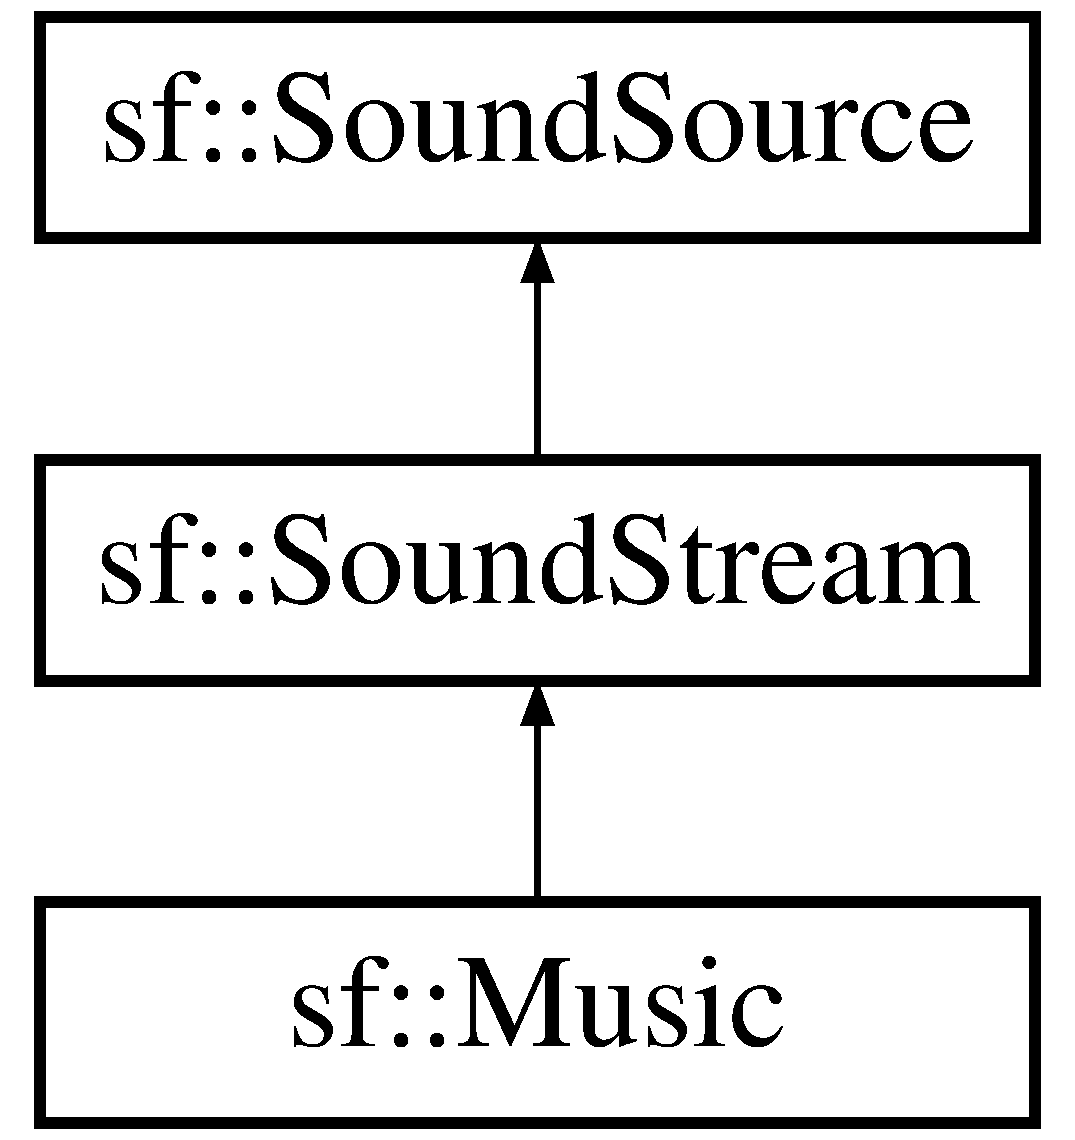
\includegraphics[height=3.000000cm]{classsf_1_1Music}
\end{center}
\end{figure}
\subsection*{Public Member Functions}
\begin{DoxyCompactItemize}
\item 
\hypertarget{classsf_1_1Music_a0bc787d8e022b3a9b89cf2c28befd42e}{\hyperlink{classsf_1_1Music_a0bc787d8e022b3a9b89cf2c28befd42e}{Music} ()}\label{classsf_1_1Music_a0bc787d8e022b3a9b89cf2c28befd42e}

\begin{DoxyCompactList}\small\item\em Default constructor. \end{DoxyCompactList}\item 
\hypertarget{classsf_1_1Music_a4c65860fed2f01d0eaa6c4199870414b}{\hyperlink{classsf_1_1Music_a4c65860fed2f01d0eaa6c4199870414b}{$\sim$\-Music} ()}\label{classsf_1_1Music_a4c65860fed2f01d0eaa6c4199870414b}

\begin{DoxyCompactList}\small\item\em Destructor. \end{DoxyCompactList}\item 
bool \hyperlink{classsf_1_1Music_a3edc66e5f5b3f11e84b90eaec9c7d7c0}{open\-From\-File} (const std\-::string \&filename)
\begin{DoxyCompactList}\small\item\em Open a music from an audio file. \end{DoxyCompactList}\item 
bool \hyperlink{classsf_1_1Music_ae93b21bcf28ff0b5fec458039111386e}{open\-From\-Memory} (const void $\ast$data, std\-::size\-\_\-t size\-In\-Bytes)
\begin{DoxyCompactList}\small\item\em Open a music from an audio file in memory. \end{DoxyCompactList}\item 
bool \hyperlink{classsf_1_1Music_a4e55d1910a26858b44778c26b237d673}{open\-From\-Stream} (\hyperlink{classsf_1_1InputStream}{Input\-Stream} \&stream)
\begin{DoxyCompactList}\small\item\em Open a music from an audio file in a custom stream. \end{DoxyCompactList}\item 
\hyperlink{classsf_1_1Time}{Time} \hyperlink{classsf_1_1Music_af4738b69c4c5038f71414ad7ffbbdc2b}{get\-Duration} () const 
\begin{DoxyCompactList}\small\item\em Get the total duration of the music. \end{DoxyCompactList}\end{DoxyCompactItemize}
\subsection*{Protected Member Functions}
\begin{DoxyCompactItemize}
\item 
virtual bool \hyperlink{classsf_1_1Music_aca1bcb4e5d56a854133e74bd86374463}{on\-Get\-Data} (\hyperlink{structsf_1_1SoundStream_1_1Chunk}{Chunk} \&data)
\begin{DoxyCompactList}\small\item\em Request a new chunk of audio samples from the stream source. \end{DoxyCompactList}\item 
virtual void \hyperlink{classsf_1_1Music_a15119cc0419c16bb334fa0698699c02e}{on\-Seek} (\hyperlink{classsf_1_1Time}{Time} time\-Offset)
\begin{DoxyCompactList}\small\item\em Change the current playing position in the stream source. \end{DoxyCompactList}\end{DoxyCompactItemize}
\subsection*{Additional Inherited Members}


\subsection{Detailed Description}
Streamed music played from an audio file. 

Musics are sounds that are streamed rather than completely loaded in memory. This is especially useful for compressed musics that usually take hundreds of M\-B when they are uncompressed\-: by streaming it instead of loading it entirely, you avoid saturating the memory and have almost no loading delay.

Apart from that, a \hyperlink{classsf_1_1Music}{sf\-::\-Music} has almost the same features as the \hyperlink{classsf_1_1SoundBuffer}{sf\-::\-Sound\-Buffer} / \hyperlink{classsf_1_1Sound}{sf\-::\-Sound} pair\-: you can play/pause/stop it, request its parameters (channels, sample rate), change the way it is played (pitch, volume, 3\-D position, ...), etc.

As a sound stream, a music is played in its own thread in order not to block the rest of the program. This means that you can leave the music alone after calling \hyperlink{classsf_1_1SoundStream_afdc08b69cab5f243d9324940a85a1144}{play()}, it will manage itself very well.

Usage example\-: 
\begin{DoxyCode}
\textcolor{comment}{// Declare a new music}
\hyperlink{classsf_1_1Music}{sf::Music} music;

\textcolor{comment}{// Open it from an audio file}
\textcolor{keywordflow}{if} (!music.\hyperlink{classsf_1_1Music_a3edc66e5f5b3f11e84b90eaec9c7d7c0}{openFromFile}(\textcolor{stringliteral}{"music.ogg"}))
\{
    \textcolor{comment}{// error...}
\}

\textcolor{comment}{// Change some parameters}
music.\hyperlink{classsf_1_1SoundSource_a0480257ea25d986eba6cc3c1a6f8d7c2}{setPosition}(0, 1, 10); \textcolor{comment}{// change its 3D position}
music.\hyperlink{classsf_1_1SoundSource_a72a13695ed48b7f7b55e7cd4431f4bb6}{setPitch}(2);           \textcolor{comment}{// increase the pitch}
music.\hyperlink{classsf_1_1SoundSource_a2f192f2b49fb8e2b82f3498d3663fcc2}{setVolume}(50);         \textcolor{comment}{// reduce the volume}
music.\hyperlink{classsf_1_1SoundStream_a43fade018ffba7e4f847a9f00b353f3d}{setLoop}(\textcolor{keyword}{true});         \textcolor{comment}{// make it loop}

\textcolor{comment}{// Play it}
music.\hyperlink{classsf_1_1SoundStream_afdc08b69cab5f243d9324940a85a1144}{play}();
\end{DoxyCode}


\begin{DoxySeeAlso}{See Also}
\hyperlink{classsf_1_1Sound}{sf\-::\-Sound}, \hyperlink{classsf_1_1SoundStream}{sf\-::\-Sound\-Stream} 
\end{DoxySeeAlso}


Definition at line 52 of file Music.\-hpp.



\subsection{Member Function Documentation}
\hypertarget{classsf_1_1Music_af4738b69c4c5038f71414ad7ffbbdc2b}{\index{sf\-::\-Music@{sf\-::\-Music}!get\-Duration@{get\-Duration}}
\index{get\-Duration@{get\-Duration}!sf::Music@{sf\-::\-Music}}
\subsubsection[{get\-Duration}]{\setlength{\rightskip}{0pt plus 5cm}{\bf Time} sf\-::\-Music\-::get\-Duration (
\begin{DoxyParamCaption}
{}
\end{DoxyParamCaption}
) const}}\label{classsf_1_1Music_af4738b69c4c5038f71414ad7ffbbdc2b}


Get the total duration of the music. 

\begin{DoxyReturn}{Returns}
\hyperlink{classsf_1_1Music}{Music} duration 
\end{DoxyReturn}
\hypertarget{classsf_1_1Music_aca1bcb4e5d56a854133e74bd86374463}{\index{sf\-::\-Music@{sf\-::\-Music}!on\-Get\-Data@{on\-Get\-Data}}
\index{on\-Get\-Data@{on\-Get\-Data}!sf::Music@{sf\-::\-Music}}
\subsubsection[{on\-Get\-Data}]{\setlength{\rightskip}{0pt plus 5cm}virtual bool sf\-::\-Music\-::on\-Get\-Data (
\begin{DoxyParamCaption}
\item[{{\bf Chunk} \&}]{data}
\end{DoxyParamCaption}
)\hspace{0.3cm}{\ttfamily [protected]}, {\ttfamily [virtual]}}}\label{classsf_1_1Music_aca1bcb4e5d56a854133e74bd86374463}


Request a new chunk of audio samples from the stream source. 

This function fills the chunk from the next samples to read from the audio file.


\begin{DoxyParams}{Parameters}
{\em data} & Chunk of data to fill\\
\hline
\end{DoxyParams}
\begin{DoxyReturn}{Returns}
True to continue playback, false to stop 
\end{DoxyReturn}


Implements \hyperlink{classsf_1_1SoundStream_a968ec024a6e45490962c8a1121cb7c5f}{sf\-::\-Sound\-Stream}.

\hypertarget{classsf_1_1Music_a15119cc0419c16bb334fa0698699c02e}{\index{sf\-::\-Music@{sf\-::\-Music}!on\-Seek@{on\-Seek}}
\index{on\-Seek@{on\-Seek}!sf::Music@{sf\-::\-Music}}
\subsubsection[{on\-Seek}]{\setlength{\rightskip}{0pt plus 5cm}virtual void sf\-::\-Music\-::on\-Seek (
\begin{DoxyParamCaption}
\item[{{\bf Time}}]{time\-Offset}
\end{DoxyParamCaption}
)\hspace{0.3cm}{\ttfamily [protected]}, {\ttfamily [virtual]}}}\label{classsf_1_1Music_a15119cc0419c16bb334fa0698699c02e}


Change the current playing position in the stream source. 


\begin{DoxyParams}{Parameters}
{\em time\-Offset} & New playing position, from the beginning of the music \\
\hline
\end{DoxyParams}


Implements \hyperlink{classsf_1_1SoundStream_a907036dd2ca7d3af5ead316e54b75997}{sf\-::\-Sound\-Stream}.

\hypertarget{classsf_1_1Music_a3edc66e5f5b3f11e84b90eaec9c7d7c0}{\index{sf\-::\-Music@{sf\-::\-Music}!open\-From\-File@{open\-From\-File}}
\index{open\-From\-File@{open\-From\-File}!sf::Music@{sf\-::\-Music}}
\subsubsection[{open\-From\-File}]{\setlength{\rightskip}{0pt plus 5cm}bool sf\-::\-Music\-::open\-From\-File (
\begin{DoxyParamCaption}
\item[{const std\-::string \&}]{filename}
\end{DoxyParamCaption}
)}}\label{classsf_1_1Music_a3edc66e5f5b3f11e84b90eaec9c7d7c0}


Open a music from an audio file. 

This function doesn't start playing the music (call \hyperlink{classsf_1_1SoundStream_afdc08b69cab5f243d9324940a85a1144}{play()} to do so). Here is a complete list of all the supported audio formats\-: ogg, wav, flac, aiff, au, raw, paf, svx, nist, voc, ircam, w64, mat4, mat5 pvf, htk, sds, avr, sd2, caf, wve, mpc2k, rf64.


\begin{DoxyParams}{Parameters}
{\em filename} & Path of the music file to open\\
\hline
\end{DoxyParams}
\begin{DoxyReturn}{Returns}
True if loading succeeded, false if it failed
\end{DoxyReturn}
\begin{DoxySeeAlso}{See Also}
\hyperlink{classsf_1_1Music_ae93b21bcf28ff0b5fec458039111386e}{open\-From\-Memory}, \hyperlink{classsf_1_1Music_a4e55d1910a26858b44778c26b237d673}{open\-From\-Stream} 
\end{DoxySeeAlso}
\hypertarget{classsf_1_1Music_ae93b21bcf28ff0b5fec458039111386e}{\index{sf\-::\-Music@{sf\-::\-Music}!open\-From\-Memory@{open\-From\-Memory}}
\index{open\-From\-Memory@{open\-From\-Memory}!sf::Music@{sf\-::\-Music}}
\subsubsection[{open\-From\-Memory}]{\setlength{\rightskip}{0pt plus 5cm}bool sf\-::\-Music\-::open\-From\-Memory (
\begin{DoxyParamCaption}
\item[{const void $\ast$}]{data, }
\item[{std\-::size\-\_\-t}]{size\-In\-Bytes}
\end{DoxyParamCaption}
)}}\label{classsf_1_1Music_ae93b21bcf28ff0b5fec458039111386e}


Open a music from an audio file in memory. 

This function doesn't start playing the music (call \hyperlink{classsf_1_1SoundStream_afdc08b69cab5f243d9324940a85a1144}{play()} to do so). Here is a complete list of all the supported audio formats\-: ogg, wav, flac, aiff, au, raw, paf, svx, nist, voc, ircam, w64, mat4, mat5 pvf, htk, sds, avr, sd2, caf, wve, mpc2k, rf64. Since the music is not loaded completely but rather streamed continuously, the {\itshape data} must remain available as long as the music is playing (ie. you can't deallocate it right after calling this function).


\begin{DoxyParams}{Parameters}
{\em data} & Pointer to the file data in memory \\
\hline
{\em size\-In\-Bytes} & Size of the data to load, in bytes\\
\hline
\end{DoxyParams}
\begin{DoxyReturn}{Returns}
True if loading succeeded, false if it failed
\end{DoxyReturn}
\begin{DoxySeeAlso}{See Also}
\hyperlink{classsf_1_1Music_a3edc66e5f5b3f11e84b90eaec9c7d7c0}{open\-From\-File}, \hyperlink{classsf_1_1Music_a4e55d1910a26858b44778c26b237d673}{open\-From\-Stream} 
\end{DoxySeeAlso}
\hypertarget{classsf_1_1Music_a4e55d1910a26858b44778c26b237d673}{\index{sf\-::\-Music@{sf\-::\-Music}!open\-From\-Stream@{open\-From\-Stream}}
\index{open\-From\-Stream@{open\-From\-Stream}!sf::Music@{sf\-::\-Music}}
\subsubsection[{open\-From\-Stream}]{\setlength{\rightskip}{0pt plus 5cm}bool sf\-::\-Music\-::open\-From\-Stream (
\begin{DoxyParamCaption}
\item[{{\bf Input\-Stream} \&}]{stream}
\end{DoxyParamCaption}
)}}\label{classsf_1_1Music_a4e55d1910a26858b44778c26b237d673}


Open a music from an audio file in a custom stream. 

This function doesn't start playing the music (call \hyperlink{classsf_1_1SoundStream_afdc08b69cab5f243d9324940a85a1144}{play()} to do so). Here is a complete list of all the supported audio formats\-: ogg, wav, flac, aiff, au, raw, paf, svx, nist, voc, ircam, w64, mat4, mat5 pvf, htk, sds, avr, sd2, caf, wve, mpc2k, rf64. Since the music is not loaded completely but rather streamed continuously, the {\itshape stream} must remain alive as long as the music is playing (ie. you can't destroy it right after calling this function).


\begin{DoxyParams}{Parameters}
{\em stream} & Source stream to read from\\
\hline
\end{DoxyParams}
\begin{DoxyReturn}{Returns}
True if loading succeeded, false if it failed
\end{DoxyReturn}
\begin{DoxySeeAlso}{See Also}
\hyperlink{classsf_1_1Music_a3edc66e5f5b3f11e84b90eaec9c7d7c0}{open\-From\-File}, \hyperlink{classsf_1_1Music_ae93b21bcf28ff0b5fec458039111386e}{open\-From\-Memory} 
\end{DoxySeeAlso}


The documentation for this class was generated from the following file\-:\begin{DoxyCompactItemize}
\item 
/home/z\-Zelman/\-Dropbox/\-Placeholder-\/\-R\-T\-S/\-S\-F\-M\-L-\/2.\-1/include/\-S\-F\-M\-L/\-Audio/Music.\-hpp\end{DoxyCompactItemize}

\hypertarget{classsf_1_1Mutex}{\section{sf\-:\-:Mutex Class Reference}
\label{classsf_1_1Mutex}\index{sf\-::\-Mutex@{sf\-::\-Mutex}}
}


Blocks concurrent access to shared resources from multiple threads.  




{\ttfamily \#include $<$Mutex.\-hpp$>$}

Inheritance diagram for sf\-:\-:Mutex\-:\begin{figure}[H]
\begin{center}
\leavevmode
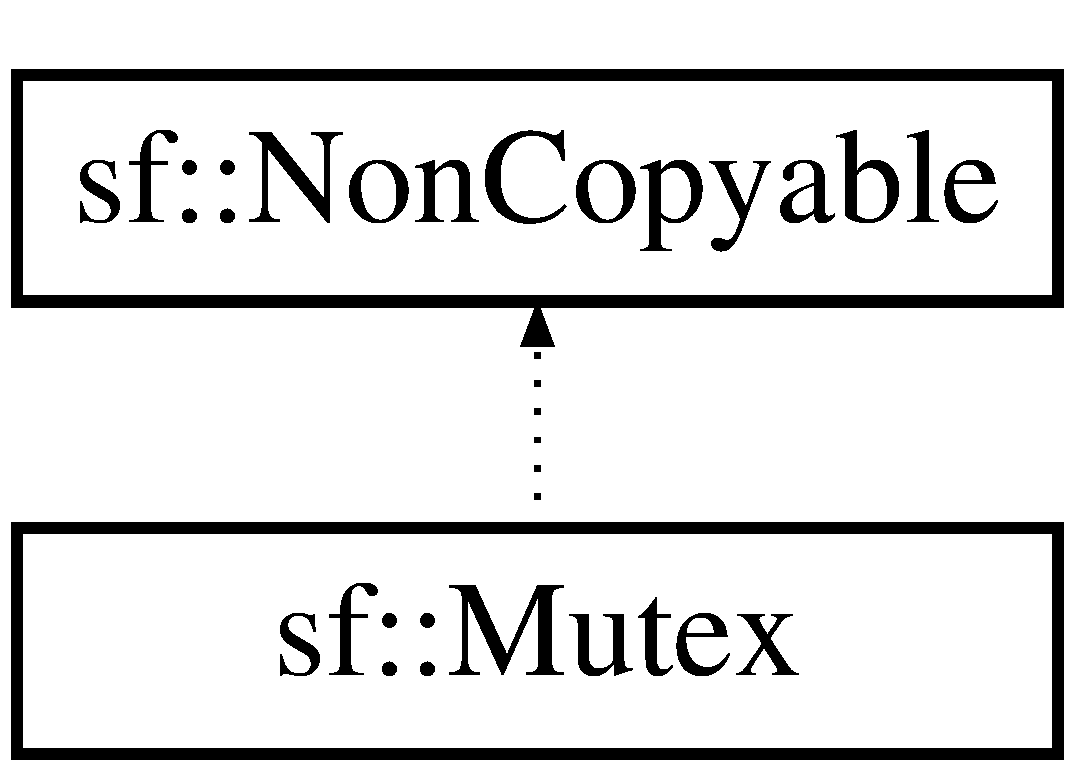
\includegraphics[height=2.000000cm]{classsf_1_1Mutex}
\end{center}
\end{figure}
\subsection*{Public Member Functions}
\begin{DoxyCompactItemize}
\item 
\hypertarget{classsf_1_1Mutex_a9bd52a48320fd7b6db8a78037aad276e}{\hyperlink{classsf_1_1Mutex_a9bd52a48320fd7b6db8a78037aad276e}{Mutex} ()}\label{classsf_1_1Mutex_a9bd52a48320fd7b6db8a78037aad276e}

\begin{DoxyCompactList}\small\item\em Default constructor. \end{DoxyCompactList}\item 
\hypertarget{classsf_1_1Mutex_a9f76a67b7b6d3918131a692179b4e3f2}{\hyperlink{classsf_1_1Mutex_a9f76a67b7b6d3918131a692179b4e3f2}{$\sim$\-Mutex} ()}\label{classsf_1_1Mutex_a9f76a67b7b6d3918131a692179b4e3f2}

\begin{DoxyCompactList}\small\item\em Destructor. \end{DoxyCompactList}\item 
void \hyperlink{classsf_1_1Mutex_a1a16956a6bbea764480c1b80f2e45763}{lock} ()
\begin{DoxyCompactList}\small\item\em \hyperlink{classsf_1_1Lock}{Lock} the mutex. \end{DoxyCompactList}\item 
void \hyperlink{classsf_1_1Mutex_ade71268ffc5e80756652058b01c23c33}{unlock} ()
\begin{DoxyCompactList}\small\item\em Unlock the mutex. \end{DoxyCompactList}\end{DoxyCompactItemize}


\subsection{Detailed Description}
Blocks concurrent access to shared resources from multiple threads. 

\hyperlink{classsf_1_1Mutex}{Mutex} stands for \char`\"{}\-M\-U\-Tual E\-Xclusion\char`\"{}. A mutex is a synchronization object, used when multiple threads are involved.

When you want to protect a part of the code from being accessed simultaneously by multiple threads, you typically use a mutex. When a thread is locked by a mutex, any other thread trying to lock it will be blocked until the mutex is released by the thread that locked it. This way, you can allow only one thread at a time to access a critical region of your code.

Usage example\-: 
\begin{DoxyCode}
Database database; \textcolor{comment}{// this is a critical resource that needs some protection}
\hyperlink{classsf_1_1Mutex}{sf::Mutex} mutex;

\textcolor{keywordtype}{void} thread1()
\{
    mutex.\hyperlink{classsf_1_1Mutex_a1a16956a6bbea764480c1b80f2e45763}{lock}(); \textcolor{comment}{// this call will block the thread if the mutex is already locked by thread2}
    database.write(...);
    mutex.\hyperlink{classsf_1_1Mutex_ade71268ffc5e80756652058b01c23c33}{unlock}(); \textcolor{comment}{// if thread2 was waiting, it will now be unblocked}
\}

\textcolor{keywordtype}{void} thread2()
\{
    mutex.\hyperlink{classsf_1_1Mutex_a1a16956a6bbea764480c1b80f2e45763}{lock}(); \textcolor{comment}{// this call will block the thread if the mutex is already locked by thread1}
    database.write(...);
    mutex.\hyperlink{classsf_1_1Mutex_ade71268ffc5e80756652058b01c23c33}{unlock}(); \textcolor{comment}{// if thread1 was waiting, it will now be unblocked}
\}
\end{DoxyCode}


Be very careful with mutexes. A bad usage can lead to bad problems, like deadlocks (two threads are waiting for each other and the application is globally stuck).

To make the usage of mutexes more robust, particularly in environments where exceptions can be thrown, you should use the helper class \hyperlink{classsf_1_1Lock}{sf\-::\-Lock} to lock/unlock mutexes.

S\-F\-M\-L mutexes are recursive, which means that you can lock a mutex multiple times in the same thread without creating a deadlock. In this case, the first call to \hyperlink{classsf_1_1Mutex_a1a16956a6bbea764480c1b80f2e45763}{lock()} behaves as usual, and the following ones have no effect. However, you must call \hyperlink{classsf_1_1Mutex_ade71268ffc5e80756652058b01c23c33}{unlock()} exactly as many times as you called \hyperlink{classsf_1_1Mutex_a1a16956a6bbea764480c1b80f2e45763}{lock()}. If you don't, the mutex won't be released.

\begin{DoxySeeAlso}{See Also}
\hyperlink{classsf_1_1Lock}{sf\-::\-Lock} 
\end{DoxySeeAlso}


Definition at line 47 of file Mutex.\-hpp.



\subsection{Member Function Documentation}
\hypertarget{classsf_1_1Mutex_a1a16956a6bbea764480c1b80f2e45763}{\index{sf\-::\-Mutex@{sf\-::\-Mutex}!lock@{lock}}
\index{lock@{lock}!sf::Mutex@{sf\-::\-Mutex}}
\subsubsection[{lock}]{\setlength{\rightskip}{0pt plus 5cm}void sf\-::\-Mutex\-::lock (
\begin{DoxyParamCaption}
{}
\end{DoxyParamCaption}
)}}\label{classsf_1_1Mutex_a1a16956a6bbea764480c1b80f2e45763}


\hyperlink{classsf_1_1Lock}{Lock} the mutex. 

If the mutex is already locked in another thread, this call will block the execution until the mutex is released.

\begin{DoxySeeAlso}{See Also}
\hyperlink{classsf_1_1Mutex_ade71268ffc5e80756652058b01c23c33}{unlock} 
\end{DoxySeeAlso}
\hypertarget{classsf_1_1Mutex_ade71268ffc5e80756652058b01c23c33}{\index{sf\-::\-Mutex@{sf\-::\-Mutex}!unlock@{unlock}}
\index{unlock@{unlock}!sf::Mutex@{sf\-::\-Mutex}}
\subsubsection[{unlock}]{\setlength{\rightskip}{0pt plus 5cm}void sf\-::\-Mutex\-::unlock (
\begin{DoxyParamCaption}
{}
\end{DoxyParamCaption}
)}}\label{classsf_1_1Mutex_ade71268ffc5e80756652058b01c23c33}


Unlock the mutex. 

\begin{DoxySeeAlso}{See Also}
\hyperlink{classsf_1_1Mutex_a1a16956a6bbea764480c1b80f2e45763}{lock} 
\end{DoxySeeAlso}


The documentation for this class was generated from the following file\-:\begin{DoxyCompactItemize}
\item 
/home/z\-Zelman/\-Dropbox/\-Placeholder-\/\-R\-T\-S/\-S\-F\-M\-L-\/2.\-1/include/\-S\-F\-M\-L/\-System/Mutex.\-hpp\end{DoxyCompactItemize}

\hypertarget{classrapidxml_1_1node__iterator}{\section{rapidxml\-:\-:node\-\_\-iterator$<$ Ch $>$ Class Template Reference}
\label{classrapidxml_1_1node__iterator}\index{rapidxml\-::node\-\_\-iterator$<$ Ch $>$@{rapidxml\-::node\-\_\-iterator$<$ Ch $>$}}
}


Iterator of child nodes of \hyperlink{classrapidxml_1_1xml__node}{xml\-\_\-node}.  




{\ttfamily \#include $<$rapidxml\-\_\-iterators.\-hpp$>$}

\subsection*{Public Types}
\begin{DoxyCompactItemize}
\item 
\hypertarget{classrapidxml_1_1node__iterator_ade6310119ed1f72c94830e006fac69b7}{typedef \hyperlink{classrapidxml_1_1xml__node}{xml\-\_\-node}$<$ Ch $>$ {\bfseries value\-\_\-type}}\label{classrapidxml_1_1node__iterator_ade6310119ed1f72c94830e006fac69b7}

\item 
\hypertarget{classrapidxml_1_1node__iterator_ad7fabbcb7d3d9e4e220299c5475b9e9c}{typedef \hyperlink{classrapidxml_1_1xml__node}{xml\-\_\-node}$<$ Ch $>$ \& {\bfseries reference}}\label{classrapidxml_1_1node__iterator_ad7fabbcb7d3d9e4e220299c5475b9e9c}

\item 
\hypertarget{classrapidxml_1_1node__iterator_a65dca8bca2b9c29f635b9ad0bdeeecb9}{typedef \hyperlink{classrapidxml_1_1xml__node}{xml\-\_\-node}$<$ Ch $>$ $\ast$ {\bfseries pointer}}\label{classrapidxml_1_1node__iterator_a65dca8bca2b9c29f635b9ad0bdeeecb9}

\item 
\hypertarget{classrapidxml_1_1node__iterator_a5bdc462b980a52c5fa2d99ac9f4f4bff}{typedef std\-::ptrdiff\-\_\-t {\bfseries difference\-\_\-type}}\label{classrapidxml_1_1node__iterator_a5bdc462b980a52c5fa2d99ac9f4f4bff}

\item 
\hypertarget{classrapidxml_1_1node__iterator_a8e82d75f768e17bf7349d010ee26c037}{typedef \\*
std\-::bidirectional\-\_\-iterator\-\_\-tag {\bfseries iterator\-\_\-category}}\label{classrapidxml_1_1node__iterator_a8e82d75f768e17bf7349d010ee26c037}

\end{DoxyCompactItemize}
\subsection*{Public Member Functions}
\begin{DoxyCompactItemize}
\item 
\hypertarget{classrapidxml_1_1node__iterator_a94c3da59b54e4bd003e226cc35b3c266}{{\bfseries node\-\_\-iterator} (\hyperlink{classrapidxml_1_1xml__node}{xml\-\_\-node}$<$ Ch $>$ $\ast$node)}\label{classrapidxml_1_1node__iterator_a94c3da59b54e4bd003e226cc35b3c266}

\item 
\hypertarget{classrapidxml_1_1node__iterator_ab31fe5bc1fd01fee8a2b31c3e42d78ed}{\hyperlink{classrapidxml_1_1xml__node}{reference} {\bfseries operator$\ast$} () const }\label{classrapidxml_1_1node__iterator_ab31fe5bc1fd01fee8a2b31c3e42d78ed}

\item 
\hypertarget{classrapidxml_1_1node__iterator_a9b3e7d58c4a628524914932e0663ddfb}{\hyperlink{classrapidxml_1_1xml__node}{pointer} {\bfseries operator-\/$>$} () const }\label{classrapidxml_1_1node__iterator_a9b3e7d58c4a628524914932e0663ddfb}

\item 
\hypertarget{classrapidxml_1_1node__iterator_a8d6b184a76b2ec8a8b5e90bc013c80ed}{\hyperlink{classrapidxml_1_1node__iterator}{node\-\_\-iterator} \& {\bfseries operator++} ()}\label{classrapidxml_1_1node__iterator_a8d6b184a76b2ec8a8b5e90bc013c80ed}

\item 
\hypertarget{classrapidxml_1_1node__iterator_ad01b4e43e348a330984833fd4924d0f2}{\hyperlink{classrapidxml_1_1node__iterator}{node\-\_\-iterator} {\bfseries operator++} (int)}\label{classrapidxml_1_1node__iterator_ad01b4e43e348a330984833fd4924d0f2}

\item 
\hypertarget{classrapidxml_1_1node__iterator_ace52107ecd1bcf02e49619e86206e3a3}{\hyperlink{classrapidxml_1_1node__iterator}{node\-\_\-iterator} \& {\bfseries operator-\/-\/} ()}\label{classrapidxml_1_1node__iterator_ace52107ecd1bcf02e49619e86206e3a3}

\item 
\hypertarget{classrapidxml_1_1node__iterator_a4ca35716bb7865f199a137b063af6080}{\hyperlink{classrapidxml_1_1node__iterator}{node\-\_\-iterator} {\bfseries operator-\/-\/} (int)}\label{classrapidxml_1_1node__iterator_a4ca35716bb7865f199a137b063af6080}

\item 
\hypertarget{classrapidxml_1_1node__iterator_a5cb8a3b0d65a1a2517995e986a4debfd}{bool {\bfseries operator==} (const \hyperlink{classrapidxml_1_1node__iterator}{node\-\_\-iterator}$<$ Ch $>$ \&rhs)}\label{classrapidxml_1_1node__iterator_a5cb8a3b0d65a1a2517995e986a4debfd}

\item 
\hypertarget{classrapidxml_1_1node__iterator_a20f1e25347d7e3856694f18597f7c8e2}{bool {\bfseries operator!=} (const \hyperlink{classrapidxml_1_1node__iterator}{node\-\_\-iterator}$<$ Ch $>$ \&rhs)}\label{classrapidxml_1_1node__iterator_a20f1e25347d7e3856694f18597f7c8e2}

\end{DoxyCompactItemize}


\subsection{Detailed Description}
\subsubsection*{template$<$class Ch$>$class rapidxml\-::node\-\_\-iterator$<$ Ch $>$}

Iterator of child nodes of \hyperlink{classrapidxml_1_1xml__node}{xml\-\_\-node}. 

Definition at line 16 of file rapidxml\-\_\-iterators.\-hpp.



The documentation for this class was generated from the following file\-:\begin{DoxyCompactItemize}
\item 
/home/z\-Zelman/\-Dropbox/\-Placeholder-\/\-R\-T\-S/rapidxml-\/1.\-13/\hyperlink{rapidxml__iterators_8hpp}{rapidxml\-\_\-iterators.\-hpp}\end{DoxyCompactItemize}

\hypertarget{classsf_1_1NonCopyable}{\section{sf\-:\-:Non\-Copyable Class Reference}
\label{classsf_1_1NonCopyable}\index{sf\-::\-Non\-Copyable@{sf\-::\-Non\-Copyable}}
}


Utility class that makes any derived class non-\/copyable.  




{\ttfamily \#include $<$Non\-Copyable.\-hpp$>$}

Inheritance diagram for sf\-:\-:Non\-Copyable\-:\begin{figure}[H]
\begin{center}
\leavevmode
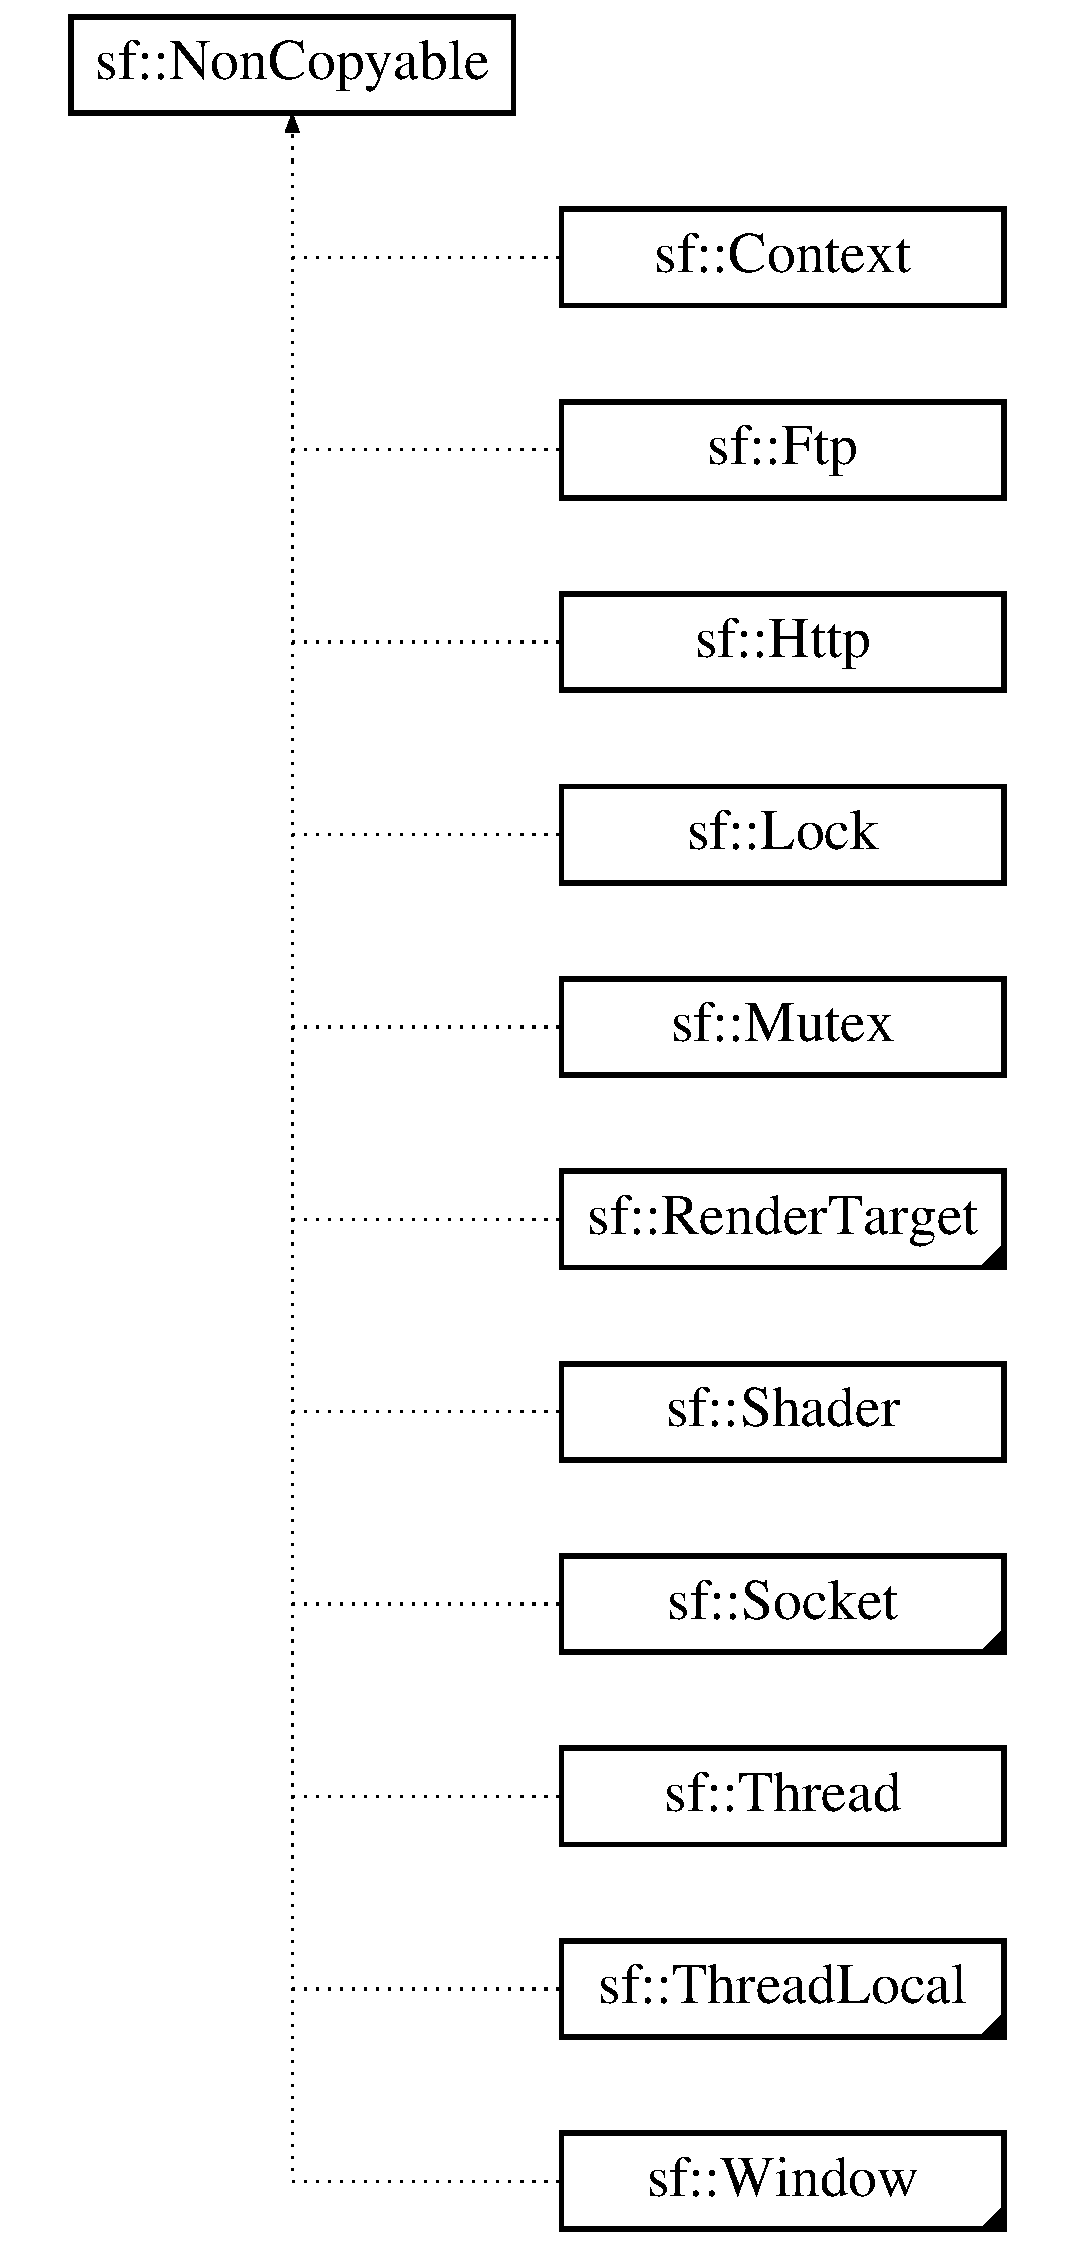
\includegraphics[height=12.000000cm]{classsf_1_1NonCopyable}
\end{center}
\end{figure}
\subsection*{Protected Member Functions}
\begin{DoxyCompactItemize}
\item 
\hyperlink{classsf_1_1NonCopyable_a2110add170580fdb946f887719da6860}{Non\-Copyable} ()
\begin{DoxyCompactList}\small\item\em Default constructor. \end{DoxyCompactList}\end{DoxyCompactItemize}


\subsection{Detailed Description}
Utility class that makes any derived class non-\/copyable. 

This class makes its instances non-\/copyable, by explicitely disabling its copy constructor and its assignment operator.

To create a non-\/copyable class, simply inherit from \hyperlink{classsf_1_1NonCopyable}{sf\-::\-Non\-Copyable}.

The type of inheritance (public or private) doesn't matter, the copy constructor and assignment operator are declared private in \hyperlink{classsf_1_1NonCopyable}{sf\-::\-Non\-Copyable} so they will end up being inaccessible in both cases. Thus you can use a shorter syntax for inheriting from it (see below).

Usage example\-: 
\begin{DoxyCode}
\textcolor{keyword}{class }MyNonCopyableClass : \hyperlink{classsf_1_1NonCopyable}{sf::NonCopyable}
\{
    ...
\};
\end{DoxyCode}


Deciding whether the instances of a class can be copied or not is a very important design choice. You are strongly encouraged to think about it before writing a class, and to use \hyperlink{classsf_1_1NonCopyable}{sf\-::\-Non\-Copyable} when necessary to prevent many potential future errors when using it. This is also a very important indication to users of your class. 

Definition at line 41 of file Non\-Copyable.\-hpp.



\subsection{Constructor \& Destructor Documentation}
\hypertarget{classsf_1_1NonCopyable_a2110add170580fdb946f887719da6860}{\index{sf\-::\-Non\-Copyable@{sf\-::\-Non\-Copyable}!Non\-Copyable@{Non\-Copyable}}
\index{Non\-Copyable@{Non\-Copyable}!sf::NonCopyable@{sf\-::\-Non\-Copyable}}
\subsubsection[{Non\-Copyable}]{\setlength{\rightskip}{0pt plus 5cm}sf\-::\-Non\-Copyable\-::\-Non\-Copyable (
\begin{DoxyParamCaption}
{}
\end{DoxyParamCaption}
)\hspace{0.3cm}{\ttfamily [inline]}, {\ttfamily [protected]}}}\label{classsf_1_1NonCopyable_a2110add170580fdb946f887719da6860}


Default constructor. 

Because this class has a copy constructor, the compiler will not automatically generate the default constructor. That's why we must define it explicitely. 

Definition at line 53 of file Non\-Copyable.\-hpp.



The documentation for this class was generated from the following file\-:\begin{DoxyCompactItemize}
\item 
/home/z\-Zelman/\-Dropbox/\-Placeholder-\/\-R\-T\-S/\-S\-F\-M\-L-\/2.\-1/include/\-S\-F\-M\-L/\-System/Non\-Copyable.\-hpp\end{DoxyCompactItemize}

\hypertarget{classsf_1_1Packet}{\section{sf\-:\-:Packet Class Reference}
\label{classsf_1_1Packet}\index{sf\-::\-Packet@{sf\-::\-Packet}}
}


Utility class to build blocks of data to transfer over the network.  




{\ttfamily \#include $<$Packet.\-hpp$>$}

\subsection*{Public Member Functions}
\begin{DoxyCompactItemize}
\item 
\hyperlink{classsf_1_1Packet_a786e5d4ced83992ceefa1799963ea858}{Packet} ()
\begin{DoxyCompactList}\small\item\em Default constructor. \end{DoxyCompactList}\item 
\hypertarget{classsf_1_1Packet_adc0490ca3c7c3d1e321bd742e5213913}{virtual \hyperlink{classsf_1_1Packet_adc0490ca3c7c3d1e321bd742e5213913}{$\sim$\-Packet} ()}\label{classsf_1_1Packet_adc0490ca3c7c3d1e321bd742e5213913}

\begin{DoxyCompactList}\small\item\em Virtual destructor. \end{DoxyCompactList}\item 
void \hyperlink{classsf_1_1Packet_a7dd6e429b87520008326c4d71f1cf011}{append} (const void $\ast$data, std\-::size\-\_\-t size\-In\-Bytes)
\begin{DoxyCompactList}\small\item\em Append data to the end of the packet. \end{DoxyCompactList}\item 
void \hyperlink{classsf_1_1Packet_a133ea8b8fe6e93c230f0d79f19a3bf0d}{clear} ()
\begin{DoxyCompactList}\small\item\em Clear the packet. \end{DoxyCompactList}\item 
const void $\ast$ \hyperlink{classsf_1_1Packet_a304ba9ec94c992710f4dfff879c6340e}{get\-Data} () const 
\begin{DoxyCompactList}\small\item\em Get a pointer to the data contained in the packet. \end{DoxyCompactList}\item 
std\-::size\-\_\-t \hyperlink{classsf_1_1Packet_a004b62aa5bafa69df8917171a3fe1fa0}{get\-Data\-Size} () const 
\begin{DoxyCompactList}\small\item\em Get the size of the data contained in the packet. \end{DoxyCompactList}\item 
bool \hyperlink{classsf_1_1Packet_aee3adfca6303f1e6bde3c62be392b945}{end\-Of\-Packet} () const 
\begin{DoxyCompactList}\small\item\em Tell if the reading position has reached the end of the packet. \end{DoxyCompactList}\item 
\hyperlink{classsf_1_1Packet_addcb990cde37859c748273d9de55e628}{operator Bool\-Type} () const 
\begin{DoxyCompactList}\small\item\em \hyperlink{classTest}{Test} the validity of the packet, for reading. \end{DoxyCompactList}\item 
\hyperlink{classsf_1_1Packet}{Packet} \& \hyperlink{classsf_1_1Packet_af8e26c63ba9bdccd262565ff0d3eeba2}{operator$>$$>$} (bool \&data)
\item 
\hypertarget{classsf_1_1Packet_a70fd5abb9095b5335b79c0cefd17b222}{\hyperlink{classsf_1_1Packet}{Packet} \& {\bfseries operator$>$$>$} (Int8 \&data)}\label{classsf_1_1Packet_a70fd5abb9095b5335b79c0cefd17b222}

\item 
\hypertarget{classsf_1_1Packet_aa67738284a7efc16c7594b358ef35510}{\hyperlink{classsf_1_1Packet}{Packet} \& {\bfseries operator$>$$>$} (Uint8 \&data)}\label{classsf_1_1Packet_aa67738284a7efc16c7594b358ef35510}

\item 
\hypertarget{classsf_1_1Packet_af82d6c4e6d74f2ca39732c1e29f30781}{\hyperlink{classsf_1_1Packet}{Packet} \& {\bfseries operator$>$$>$} (Int16 \&data)}\label{classsf_1_1Packet_af82d6c4e6d74f2ca39732c1e29f30781}

\item 
\hypertarget{classsf_1_1Packet_afd8706f092bc830ebb438aeee9271647}{\hyperlink{classsf_1_1Packet}{Packet} \& {\bfseries operator$>$$>$} (Uint16 \&data)}\label{classsf_1_1Packet_afd8706f092bc830ebb438aeee9271647}

\item 
\hypertarget{classsf_1_1Packet_ae7b44e79f12d500b63f5dc2a10d78d8c}{\hyperlink{classsf_1_1Packet}{Packet} \& {\bfseries operator$>$$>$} (Int32 \&data)}\label{classsf_1_1Packet_ae7b44e79f12d500b63f5dc2a10d78d8c}

\item 
\hypertarget{classsf_1_1Packet_a4b57e1953db5bec39a851929df9a339a}{\hyperlink{classsf_1_1Packet}{Packet} \& {\bfseries operator$>$$>$} (Uint32 \&data)}\label{classsf_1_1Packet_a4b57e1953db5bec39a851929df9a339a}

\item 
\hypertarget{classsf_1_1Packet_a6704b4d13d6f798efe6fa836a8b5fa24}{\hyperlink{classsf_1_1Packet}{Packet} \& {\bfseries operator$>$$>$} (float \&data)}\label{classsf_1_1Packet_a6704b4d13d6f798efe6fa836a8b5fa24}

\item 
\hypertarget{classsf_1_1Packet_ac84239a8ba0a165394805c17b35a88cf}{\hyperlink{classsf_1_1Packet}{Packet} \& {\bfseries operator$>$$>$} (double \&data)}\label{classsf_1_1Packet_ac84239a8ba0a165394805c17b35a88cf}

\item 
\hypertarget{classsf_1_1Packet_ae9f8d8b0c776204f79f615b1e58bccec}{\hyperlink{classsf_1_1Packet}{Packet} \& {\bfseries operator$>$$>$} (char $\ast$data)}\label{classsf_1_1Packet_ae9f8d8b0c776204f79f615b1e58bccec}

\item 
\hypertarget{classsf_1_1Packet_aabace32063c44e1a5cc54af6267c1fab}{\hyperlink{classsf_1_1Packet}{Packet} \& {\bfseries operator$>$$>$} (std\-::string \&data)}\label{classsf_1_1Packet_aabace32063c44e1a5cc54af6267c1fab}

\item 
\hypertarget{classsf_1_1Packet_a1444500d29df0991e630ac78933c6282}{\hyperlink{classsf_1_1Packet}{Packet} \& {\bfseries operator$>$$>$} (wchar\-\_\-t $\ast$data)}\label{classsf_1_1Packet_a1444500d29df0991e630ac78933c6282}

\item 
\hypertarget{classsf_1_1Packet_ab74c37a290385fd7b1f962bf954a2005}{\hyperlink{classsf_1_1Packet}{Packet} \& {\bfseries operator$>$$>$} (std\-::wstring \&data)}\label{classsf_1_1Packet_ab74c37a290385fd7b1f962bf954a2005}

\item 
\hypertarget{classsf_1_1Packet_a081233e0cab2182a219b129a1383dc0b}{\hyperlink{classsf_1_1Packet}{Packet} \& {\bfseries operator$>$$>$} (\hyperlink{classsf_1_1String}{String} \&data)}\label{classsf_1_1Packet_a081233e0cab2182a219b129a1383dc0b}

\item 
\hyperlink{classsf_1_1Packet}{Packet} \& \hyperlink{classsf_1_1Packet_aa5a465ed02ba29d83ecdafb0ac3fff21}{operator$<$$<$} (bool data)
\item 
\hypertarget{classsf_1_1Packet_a034b68a4281cae0b53a43af7aa4172f6}{\hyperlink{classsf_1_1Packet}{Packet} \& {\bfseries operator$<$$<$} (Int8 data)}\label{classsf_1_1Packet_a034b68a4281cae0b53a43af7aa4172f6}

\item 
\hypertarget{classsf_1_1Packet_af27e4498bf83151b0591d5f04a8b30e1}{\hyperlink{classsf_1_1Packet}{Packet} \& {\bfseries operator$<$$<$} (Uint8 data)}\label{classsf_1_1Packet_af27e4498bf83151b0591d5f04a8b30e1}

\item 
\hypertarget{classsf_1_1Packet_afda8754ab4f2a34600f0153ba9ff24fa}{\hyperlink{classsf_1_1Packet}{Packet} \& {\bfseries operator$<$$<$} (Int16 data)}\label{classsf_1_1Packet_afda8754ab4f2a34600f0153ba9ff24fa}

\item 
\hypertarget{classsf_1_1Packet_a557cbc0289135209248aca1aa2117c40}{\hyperlink{classsf_1_1Packet}{Packet} \& {\bfseries operator$<$$<$} (Uint16 data)}\label{classsf_1_1Packet_a557cbc0289135209248aca1aa2117c40}

\item 
\hypertarget{classsf_1_1Packet_ad60c9ad6e4e92399e2a36938ad122d05}{\hyperlink{classsf_1_1Packet}{Packet} \& {\bfseries operator$<$$<$} (Int32 data)}\label{classsf_1_1Packet_ad60c9ad6e4e92399e2a36938ad122d05}

\item 
\hypertarget{classsf_1_1Packet_afb113b73749efb662a75deb98257ad34}{\hyperlink{classsf_1_1Packet}{Packet} \& {\bfseries operator$<$$<$} (Uint32 data)}\label{classsf_1_1Packet_afb113b73749efb662a75deb98257ad34}

\item 
\hypertarget{classsf_1_1Packet_a76d31c4f864253a7e9b53701b4660fe5}{\hyperlink{classsf_1_1Packet}{Packet} \& {\bfseries operator$<$$<$} (float data)}\label{classsf_1_1Packet_a76d31c4f864253a7e9b53701b4660fe5}

\item 
\hypertarget{classsf_1_1Packet_a3b3077720a486b569ac8e7dec638a3f0}{\hyperlink{classsf_1_1Packet}{Packet} \& {\bfseries operator$<$$<$} (double data)}\label{classsf_1_1Packet_a3b3077720a486b569ac8e7dec638a3f0}

\item 
\hypertarget{classsf_1_1Packet_a67c9985f7b3d6e90886e56e309280a9d}{\hyperlink{classsf_1_1Packet}{Packet} \& {\bfseries operator$<$$<$} (const char $\ast$data)}\label{classsf_1_1Packet_a67c9985f7b3d6e90886e56e309280a9d}

\item 
\hypertarget{classsf_1_1Packet_a59a21671caaa69da5d47c54b50e1eb54}{\hyperlink{classsf_1_1Packet}{Packet} \& {\bfseries operator$<$$<$} (const std\-::string \&data)}\label{classsf_1_1Packet_a59a21671caaa69da5d47c54b50e1eb54}

\item 
\hypertarget{classsf_1_1Packet_a6f7c6a9ce795fac342ea937896d98016}{\hyperlink{classsf_1_1Packet}{Packet} \& {\bfseries operator$<$$<$} (const wchar\-\_\-t $\ast$data)}\label{classsf_1_1Packet_a6f7c6a9ce795fac342ea937896d98016}

\item 
\hypertarget{classsf_1_1Packet_a9f3401d038470f629d0c2c6be928a14b}{\hyperlink{classsf_1_1Packet}{Packet} \& {\bfseries operator$<$$<$} (const std\-::wstring \&data)}\label{classsf_1_1Packet_a9f3401d038470f629d0c2c6be928a14b}

\item 
\hypertarget{classsf_1_1Packet_abc17272df082a36b202e10045bd9e220}{\hyperlink{classsf_1_1Packet}{Packet} \& {\bfseries operator$<$$<$} (const \hyperlink{classsf_1_1String}{String} \&data)}\label{classsf_1_1Packet_abc17272df082a36b202e10045bd9e220}

\end{DoxyCompactItemize}
\subsection*{Protected Member Functions}
\begin{DoxyCompactItemize}
\item 
virtual const void $\ast$ \hyperlink{classsf_1_1Packet_a052e955906c9bfd671622cb625380edc}{on\-Send} (std\-::size\-\_\-t \&size)
\begin{DoxyCompactList}\small\item\em Called before the packet is sent over the network. \end{DoxyCompactList}\item 
virtual void \hyperlink{classsf_1_1Packet_ab71a31ef0f1d5d856de6f9fc75434128}{on\-Receive} (const void $\ast$data, std\-::size\-\_\-t size)
\begin{DoxyCompactList}\small\item\em Called after the packet is received over the network. \end{DoxyCompactList}\end{DoxyCompactItemize}
\subsection*{Friends}
\begin{DoxyCompactItemize}
\item 
\hypertarget{classsf_1_1Packet_aa8b32310b01d4bb702d6bcb969d5f130}{class {\bfseries Tcp\-Socket}}\label{classsf_1_1Packet_aa8b32310b01d4bb702d6bcb969d5f130}

\item 
\hypertarget{classsf_1_1Packet_ae128c6687ced82c6157c5f865f8dec5c}{class {\bfseries Udp\-Socket}}\label{classsf_1_1Packet_ae128c6687ced82c6157c5f865f8dec5c}

\end{DoxyCompactItemize}


\subsection{Detailed Description}
Utility class to build blocks of data to transfer over the network. 

Packets provide a safe and easy way to serialize data, in order to send it over the network using sockets (\hyperlink{classsf_1_1TcpSocket}{sf\-::\-Tcp\-Socket}, \hyperlink{classsf_1_1UdpSocket}{sf\-::\-Udp\-Socket}).

Packets solve 2 fundamental problems that arise when transfering data over the network\-: \begin{DoxyItemize}
\item data is interpreted correctly according to the endianness \item the bounds of the packet are preserved (one send == one receive)\end{DoxyItemize}
The \hyperlink{classsf_1_1Packet}{sf\-::\-Packet} class provides both input and output modes. It is designed to follow the behaviour of standard C++ streams, using operators $>$$>$ and $<$$<$ to extract and insert data.

It is recommended to use only fixed-\/size types (like sf\-::\-Int32, etc.), to avoid possible differences between the sender and the receiver. Indeed, the native C++ types may have different sizes on two platforms and your data may be corrupted if that happens.

Usage example\-: 
\begin{DoxyCode}
sf::Uint32 x = 24;
std::string s = \textcolor{stringliteral}{"hello"};
\textcolor{keywordtype}{double} d = 5.89;

\textcolor{comment}{// Group the variables to send into a packet}
\hyperlink{classsf_1_1Packet}{sf::Packet} packet;
packet << x << s << d;

\textcolor{comment}{// Send it over the network (socket is a valid sf::TcpSocket)}
socket.send(packet);

-----------------------------------------------------------------

\textcolor{comment}{// Receive the packet at the other end}
\hyperlink{classsf_1_1Packet}{sf::Packet} packet;
socket.receive(packet);

\textcolor{comment}{// Extract the variables contained in the packet}
sf::Uint32 x;
std::string s;
\textcolor{keywordtype}{double} d;
\textcolor{keywordflow}{if} (packet >> x >> s >> d)
\{
    \textcolor{comment}{// Data extracted successfully...}
\}
\end{DoxyCode}


Packets have built-\/in operator $>$$>$ and $<$$<$ overloads for standard types\-: \begin{DoxyItemize}
\item bool \item fixed-\/size integer types (sf\-::\-Int8/16/32, sf\-::\-Uint8/16/32) \item floating point numbers (float, double) \item string types (char$\ast$, wchar\-\_\-t$\ast$, std\-::string, std\-::wstring, \hyperlink{classsf_1_1String}{sf\-::\-String})\end{DoxyItemize}
Like standard streams, it is also possible to define your own overloads of operators $>$$>$ and $<$$<$ in order to handle your custom types.


\begin{DoxyCode}
\textcolor{keyword}{struct }MyStruct
\{
    \textcolor{keywordtype}{float}       number;
    sf::Int8    integer;
    std::string str;
\};

\hyperlink{classsf_1_1Packet}{sf::Packet}& \hyperlink{classsf_1_1Packet_aa5a465ed02ba29d83ecdafb0ac3fff21}{operator <<}(\hyperlink{classsf_1_1Packet}{sf::Packet}& packet, \textcolor{keyword}{const} MyStruct& m)
\{
    \textcolor{keywordflow}{return} packet << m.number << m.integer << m.str;
\}

\hyperlink{classsf_1_1Packet}{sf::Packet}& \hyperlink{classsf_1_1Packet_af8e26c63ba9bdccd262565ff0d3eeba2}{operator >>}(\hyperlink{classsf_1_1Packet}{sf::Packet}& packet, MyStruct& m)
\{
    \textcolor{keywordflow}{return} packet >> m.number >> m.integer >> m.str;
\}
\end{DoxyCode}


Packets also provide an extra feature that allows to apply custom transformations to the data before it is sent, and after it is received. This is typically used to handle automatic compression or encryption of the data. This is achieved by inheriting from \hyperlink{classsf_1_1Packet}{sf\-::\-Packet}, and overriding the on\-Send and on\-Receive functions.

Here is an example\-: 
\begin{DoxyCode}
\textcolor{keyword}{class }ZipPacket : \textcolor{keyword}{public} \hyperlink{classsf_1_1Packet}{sf::Packet}
\{
    \textcolor{keyword}{virtual} \textcolor{keyword}{const} \textcolor{keywordtype}{void}* \hyperlink{classsf_1_1Packet_a052e955906c9bfd671622cb625380edc}{onSend}(std::size\_t& size)
    \{
        \textcolor{keyword}{const} \textcolor{keywordtype}{void}* srcData = \hyperlink{classsf_1_1Packet_a304ba9ec94c992710f4dfff879c6340e}{getData}();
        std::size\_t srcSize = \hyperlink{classsf_1_1Packet_a004b62aa5bafa69df8917171a3fe1fa0}{getDataSize}();

        \textcolor{keywordflow}{return} MySuperZipFunction(srcData, srcSize, &size);
    \}

    \textcolor{keyword}{virtual} \textcolor{keywordtype}{void} \hyperlink{classsf_1_1Packet_ab71a31ef0f1d5d856de6f9fc75434128}{onReceive}(\textcolor{keyword}{const} \textcolor{keywordtype}{void}* data, std::size\_t size)
    \{
        std::size\_t dstSize;
        \textcolor{keyword}{const} \textcolor{keywordtype}{void}* dstData = MySuperUnzipFunction(data, size, &dstSize);

        \hyperlink{classsf_1_1Packet_a7dd6e429b87520008326c4d71f1cf011}{append}(dstData, dstSize);
    \}
\};

\textcolor{comment}{// Use like regular packets:}
ZipPacket packet;
packet << x << s << d;
...
\end{DoxyCode}


\begin{DoxySeeAlso}{See Also}
\hyperlink{classsf_1_1TcpSocket}{sf\-::\-Tcp\-Socket}, \hyperlink{classsf_1_1UdpSocket}{sf\-::\-Udp\-Socket} 
\end{DoxySeeAlso}


Definition at line 47 of file Packet.\-hpp.



\subsection{Constructor \& Destructor Documentation}
\hypertarget{classsf_1_1Packet_a786e5d4ced83992ceefa1799963ea858}{\index{sf\-::\-Packet@{sf\-::\-Packet}!Packet@{Packet}}
\index{Packet@{Packet}!sf::Packet@{sf\-::\-Packet}}
\subsubsection[{Packet}]{\setlength{\rightskip}{0pt plus 5cm}sf\-::\-Packet\-::\-Packet (
\begin{DoxyParamCaption}
{}
\end{DoxyParamCaption}
)}}\label{classsf_1_1Packet_a786e5d4ced83992ceefa1799963ea858}


Default constructor. 

Creates an empty packet. 

\subsection{Member Function Documentation}
\hypertarget{classsf_1_1Packet_a7dd6e429b87520008326c4d71f1cf011}{\index{sf\-::\-Packet@{sf\-::\-Packet}!append@{append}}
\index{append@{append}!sf::Packet@{sf\-::\-Packet}}
\subsubsection[{append}]{\setlength{\rightskip}{0pt plus 5cm}void sf\-::\-Packet\-::append (
\begin{DoxyParamCaption}
\item[{const void $\ast$}]{data, }
\item[{std\-::size\-\_\-t}]{size\-In\-Bytes}
\end{DoxyParamCaption}
)}}\label{classsf_1_1Packet_a7dd6e429b87520008326c4d71f1cf011}


Append data to the end of the packet. 


\begin{DoxyParams}{Parameters}
{\em data} & Pointer to the sequence of bytes to append \\
\hline
{\em size\-In\-Bytes} & Number of bytes to append\\
\hline
\end{DoxyParams}
\begin{DoxySeeAlso}{See Also}
\hyperlink{classsf_1_1Packet_a133ea8b8fe6e93c230f0d79f19a3bf0d}{clear} 
\end{DoxySeeAlso}
\hypertarget{classsf_1_1Packet_a133ea8b8fe6e93c230f0d79f19a3bf0d}{\index{sf\-::\-Packet@{sf\-::\-Packet}!clear@{clear}}
\index{clear@{clear}!sf::Packet@{sf\-::\-Packet}}
\subsubsection[{clear}]{\setlength{\rightskip}{0pt plus 5cm}void sf\-::\-Packet\-::clear (
\begin{DoxyParamCaption}
{}
\end{DoxyParamCaption}
)}}\label{classsf_1_1Packet_a133ea8b8fe6e93c230f0d79f19a3bf0d}


Clear the packet. 

After calling Clear, the packet is empty.

\begin{DoxySeeAlso}{See Also}
\hyperlink{classsf_1_1Packet_a7dd6e429b87520008326c4d71f1cf011}{append} 
\end{DoxySeeAlso}
\hypertarget{classsf_1_1Packet_aee3adfca6303f1e6bde3c62be392b945}{\index{sf\-::\-Packet@{sf\-::\-Packet}!end\-Of\-Packet@{end\-Of\-Packet}}
\index{end\-Of\-Packet@{end\-Of\-Packet}!sf::Packet@{sf\-::\-Packet}}
\subsubsection[{end\-Of\-Packet}]{\setlength{\rightskip}{0pt plus 5cm}bool sf\-::\-Packet\-::end\-Of\-Packet (
\begin{DoxyParamCaption}
{}
\end{DoxyParamCaption}
) const}}\label{classsf_1_1Packet_aee3adfca6303f1e6bde3c62be392b945}


Tell if the reading position has reached the end of the packet. 

This function is useful to know if there is some data left to be read, without actually reading it.

\begin{DoxyReturn}{Returns}
True if all data was read, false otherwise
\end{DoxyReturn}
\begin{DoxySeeAlso}{See Also}
operator bool 
\end{DoxySeeAlso}
\hypertarget{classsf_1_1Packet_a304ba9ec94c992710f4dfff879c6340e}{\index{sf\-::\-Packet@{sf\-::\-Packet}!get\-Data@{get\-Data}}
\index{get\-Data@{get\-Data}!sf::Packet@{sf\-::\-Packet}}
\subsubsection[{get\-Data}]{\setlength{\rightskip}{0pt plus 5cm}const void$\ast$ sf\-::\-Packet\-::get\-Data (
\begin{DoxyParamCaption}
{}
\end{DoxyParamCaption}
) const}}\label{classsf_1_1Packet_a304ba9ec94c992710f4dfff879c6340e}


Get a pointer to the data contained in the packet. 

Warning\-: the returned pointer may become invalid after you append data to the packet, therefore it should never be stored. The return pointer is N\-U\-L\-L if the packet is empty.

\begin{DoxyReturn}{Returns}
Pointer to the data
\end{DoxyReturn}
\begin{DoxySeeAlso}{See Also}
\hyperlink{classsf_1_1Packet_a004b62aa5bafa69df8917171a3fe1fa0}{get\-Data\-Size} 
\end{DoxySeeAlso}
\hypertarget{classsf_1_1Packet_a004b62aa5bafa69df8917171a3fe1fa0}{\index{sf\-::\-Packet@{sf\-::\-Packet}!get\-Data\-Size@{get\-Data\-Size}}
\index{get\-Data\-Size@{get\-Data\-Size}!sf::Packet@{sf\-::\-Packet}}
\subsubsection[{get\-Data\-Size}]{\setlength{\rightskip}{0pt plus 5cm}std\-::size\-\_\-t sf\-::\-Packet\-::get\-Data\-Size (
\begin{DoxyParamCaption}
{}
\end{DoxyParamCaption}
) const}}\label{classsf_1_1Packet_a004b62aa5bafa69df8917171a3fe1fa0}


Get the size of the data contained in the packet. 

This function returns the number of bytes pointed to by what get\-Data returns.

\begin{DoxyReturn}{Returns}
Data size, in bytes
\end{DoxyReturn}
\begin{DoxySeeAlso}{See Also}
\hyperlink{classsf_1_1Packet_a304ba9ec94c992710f4dfff879c6340e}{get\-Data} 
\end{DoxySeeAlso}
\hypertarget{classsf_1_1Packet_ab71a31ef0f1d5d856de6f9fc75434128}{\index{sf\-::\-Packet@{sf\-::\-Packet}!on\-Receive@{on\-Receive}}
\index{on\-Receive@{on\-Receive}!sf::Packet@{sf\-::\-Packet}}
\subsubsection[{on\-Receive}]{\setlength{\rightskip}{0pt plus 5cm}virtual void sf\-::\-Packet\-::on\-Receive (
\begin{DoxyParamCaption}
\item[{const void $\ast$}]{data, }
\item[{std\-::size\-\_\-t}]{size}
\end{DoxyParamCaption}
)\hspace{0.3cm}{\ttfamily [protected]}, {\ttfamily [virtual]}}}\label{classsf_1_1Packet_ab71a31ef0f1d5d856de6f9fc75434128}


Called after the packet is received over the network. 

This function can be defined by derived classes to transform the data after it is received; this can be used for uncompression, decryption, etc. The function receives a pointer to the received data, and must fill the packet with the transformed bytes. The default implementation fills the packet directly without transforming the data.


\begin{DoxyParams}{Parameters}
{\em data} & Pointer to the received bytes \\
\hline
{\em size} & Number of bytes\\
\hline
\end{DoxyParams}
\begin{DoxySeeAlso}{See Also}
\hyperlink{classsf_1_1Packet_a052e955906c9bfd671622cb625380edc}{on\-Send} 
\end{DoxySeeAlso}
\hypertarget{classsf_1_1Packet_a052e955906c9bfd671622cb625380edc}{\index{sf\-::\-Packet@{sf\-::\-Packet}!on\-Send@{on\-Send}}
\index{on\-Send@{on\-Send}!sf::Packet@{sf\-::\-Packet}}
\subsubsection[{on\-Send}]{\setlength{\rightskip}{0pt plus 5cm}virtual const void$\ast$ sf\-::\-Packet\-::on\-Send (
\begin{DoxyParamCaption}
\item[{std\-::size\-\_\-t \&}]{size}
\end{DoxyParamCaption}
)\hspace{0.3cm}{\ttfamily [protected]}, {\ttfamily [virtual]}}}\label{classsf_1_1Packet_a052e955906c9bfd671622cb625380edc}


Called before the packet is sent over the network. 

This function can be defined by derived classes to transform the data before it is sent; this can be used for compression, encryption, etc. The function must return a pointer to the modified data, as well as the number of bytes pointed. The default implementation provides the packet's data without transforming it.


\begin{DoxyParams}{Parameters}
{\em size} & Variable to fill with the size of data to send\\
\hline
\end{DoxyParams}
\begin{DoxyReturn}{Returns}
Pointer to the array of bytes to send
\end{DoxyReturn}
\begin{DoxySeeAlso}{See Also}
\hyperlink{classsf_1_1Packet_ab71a31ef0f1d5d856de6f9fc75434128}{on\-Receive} 
\end{DoxySeeAlso}
\hypertarget{classsf_1_1Packet_addcb990cde37859c748273d9de55e628}{\index{sf\-::\-Packet@{sf\-::\-Packet}!operator Bool\-Type@{operator Bool\-Type}}
\index{operator Bool\-Type@{operator Bool\-Type}!sf::Packet@{sf\-::\-Packet}}
\subsubsection[{operator Bool\-Type}]{\setlength{\rightskip}{0pt plus 5cm}sf\-::\-Packet\-::operator Bool\-Type (
\begin{DoxyParamCaption}
{}
\end{DoxyParamCaption}
) const}}\label{classsf_1_1Packet_addcb990cde37859c748273d9de55e628}


\hyperlink{classTest}{Test} the validity of the packet, for reading. 

This operator allows to test the packet as a boolean variable, to check if a reading operation was successful.

A packet will be in an invalid state if it has no more data to read.

This behaviour is the same as standard C++ streams.

Usage example\-: 
\begin{DoxyCode}
\textcolor{keywordtype}{float} x;
packet >> x;
\textcolor{keywordflow}{if} (packet)
\{
   \textcolor{comment}{// ok, x was extracted successfully}
\}

\textcolor{comment}{// -- or --}

\textcolor{keywordtype}{float} x;
\textcolor{keywordflow}{if} (packet >> x)
\{
   \textcolor{comment}{// ok, x was extracted successfully}
\}
\end{DoxyCode}


Don't focus on the return type, it's equivalent to bool but it disallows unwanted implicit conversions to integer or pointer types.

\begin{DoxyReturn}{Returns}
True if last data extraction from packet was successful
\end{DoxyReturn}
\begin{DoxySeeAlso}{See Also}
\hyperlink{classsf_1_1Packet_aee3adfca6303f1e6bde3c62be392b945}{end\-Of\-Packet} 
\end{DoxySeeAlso}
\hypertarget{classsf_1_1Packet_aa5a465ed02ba29d83ecdafb0ac3fff21}{\index{sf\-::\-Packet@{sf\-::\-Packet}!operator$<$$<$@{operator$<$$<$}}
\index{operator$<$$<$@{operator$<$$<$}!sf::Packet@{sf\-::\-Packet}}
\subsubsection[{operator$<$$<$}]{\setlength{\rightskip}{0pt plus 5cm}{\bf Packet}\& sf\-::\-Packet\-::operator$<$$<$ (
\begin{DoxyParamCaption}
\item[{bool}]{data}
\end{DoxyParamCaption}
)}}\label{classsf_1_1Packet_aa5a465ed02ba29d83ecdafb0ac3fff21}
Overloads of operator $<$$<$ to write data into the packet \hypertarget{classsf_1_1Packet_af8e26c63ba9bdccd262565ff0d3eeba2}{\index{sf\-::\-Packet@{sf\-::\-Packet}!operator$>$$>$@{operator$>$$>$}}
\index{operator$>$$>$@{operator$>$$>$}!sf::Packet@{sf\-::\-Packet}}
\subsubsection[{operator$>$$>$}]{\setlength{\rightskip}{0pt plus 5cm}{\bf Packet}\& sf\-::\-Packet\-::operator$>$$>$ (
\begin{DoxyParamCaption}
\item[{bool \&}]{data}
\end{DoxyParamCaption}
)}}\label{classsf_1_1Packet_af8e26c63ba9bdccd262565ff0d3eeba2}
Overloads of operator $>$$>$ to read data from the packet 

The documentation for this class was generated from the following file\-:\begin{DoxyCompactItemize}
\item 
/home/z\-Zelman/\-Dropbox/\-Placeholder-\/\-R\-T\-S/\-S\-F\-M\-L-\/2.\-1/include/\-S\-F\-M\-L/\-Network/Packet.\-hpp\end{DoxyCompactItemize}

\hypertarget{classrapidxml_1_1parse__error}{\section{rapidxml\-:\-:parse\-\_\-error Class Reference}
\label{classrapidxml_1_1parse__error}\index{rapidxml\-::parse\-\_\-error@{rapidxml\-::parse\-\_\-error}}
}


{\ttfamily \#include $<$rapidxml.\-hpp$>$}

Inheritance diagram for rapidxml\-:\-:parse\-\_\-error\-:\begin{figure}[H]
\begin{center}
\leavevmode
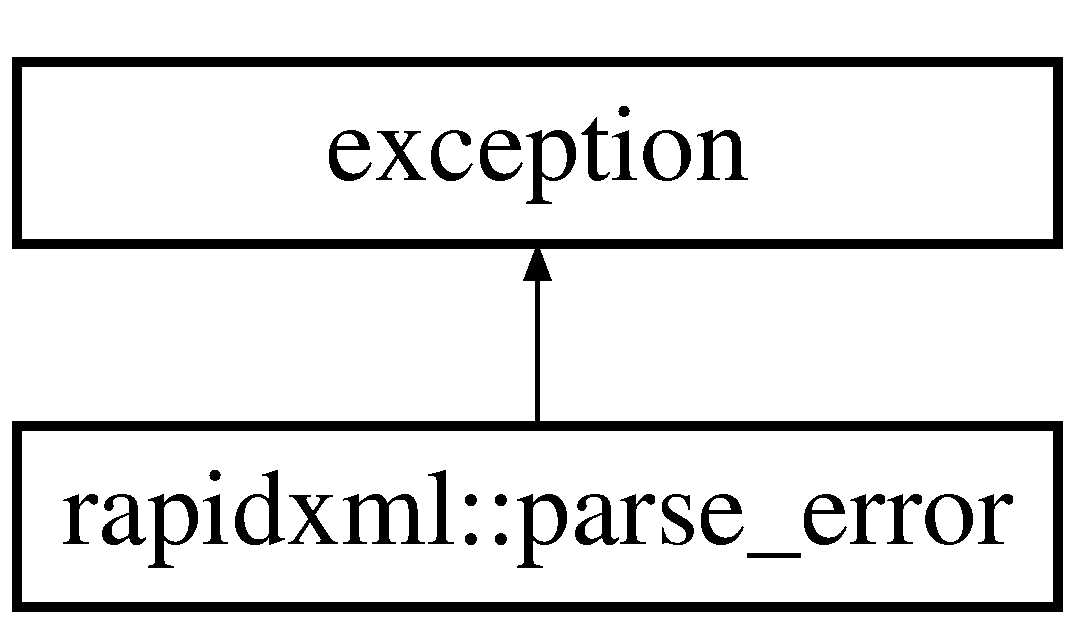
\includegraphics[height=2.000000cm]{classrapidxml_1_1parse__error}
\end{center}
\end{figure}
\subsection*{Public Member Functions}
\begin{DoxyCompactItemize}
\item 
\hypertarget{classrapidxml_1_1parse__error_aea12a301271c393fb627b368fb9f35c1}{\hyperlink{classrapidxml_1_1parse__error_aea12a301271c393fb627b368fb9f35c1}{parse\-\_\-error} (const char $\ast$\hyperlink{classrapidxml_1_1parse__error_a7665c88639e7466ee1de388a4f85e6fe}{what}, void $\ast$\hyperlink{classrapidxml_1_1parse__error_a3a0ab9e586c1d2b437c340f6622fbec6}{where})}\label{classrapidxml_1_1parse__error_aea12a301271c393fb627b368fb9f35c1}

\begin{DoxyCompactList}\small\item\em Constructs parse error. \end{DoxyCompactList}\item 
virtual const char $\ast$ \hyperlink{classrapidxml_1_1parse__error_a7665c88639e7466ee1de388a4f85e6fe}{what} () const   throw ()
\item 
{\footnotesize template$<$class Ch $>$ }\\Ch $\ast$ \hyperlink{classrapidxml_1_1parse__error_a3a0ab9e586c1d2b437c340f6622fbec6}{where} () const 
\end{DoxyCompactItemize}


\subsection{Detailed Description}
Parse error exception. This exception is thrown by the parser when an error occurs. Use \hyperlink{classrapidxml_1_1parse__error_a7665c88639e7466ee1de388a4f85e6fe}{what()} function to get human-\/readable error message. Use \hyperlink{classrapidxml_1_1parse__error_a3a0ab9e586c1d2b437c340f6622fbec6}{where()} function to get a pointer to position within source text where error was detected. \par
\par
 If throwing exceptions by the parser is undesirable, it can be disabled by defining R\-A\-P\-I\-D\-X\-M\-L\-\_\-\-N\-O\-\_\-\-E\-X\-C\-E\-P\-T\-I\-O\-N\-S macro before \hyperlink{rapidxml_8hpp}{rapidxml.\-hpp} is included. This will cause the parser to call rapidxml\-::parse\-\_\-error\-\_\-handler() function instead of throwing an exception. This function must be defined by the user. \par
\par
 This class derives from {\ttfamily std\-::exception} class. 

Definition at line 71 of file rapidxml.\-hpp.



\subsection{Member Function Documentation}
\hypertarget{classrapidxml_1_1parse__error_a7665c88639e7466ee1de388a4f85e6fe}{\index{rapidxml\-::parse\-\_\-error@{rapidxml\-::parse\-\_\-error}!what@{what}}
\index{what@{what}!rapidxml::parse_error@{rapidxml\-::parse\-\_\-error}}
\subsubsection[{what}]{\setlength{\rightskip}{0pt plus 5cm}virtual const char$\ast$ rapidxml\-::parse\-\_\-error\-::what (
\begin{DoxyParamCaption}
{}
\end{DoxyParamCaption}
) const throw  ) \hspace{0.3cm}{\ttfamily [inline]}, {\ttfamily [virtual]}}}\label{classrapidxml_1_1parse__error_a7665c88639e7466ee1de388a4f85e6fe}
Gets human readable description of error. \begin{DoxyReturn}{Returns}
Pointer to null terminated description of the error. 
\end{DoxyReturn}


Definition at line 85 of file rapidxml.\-hpp.

\hypertarget{classrapidxml_1_1parse__error_a3a0ab9e586c1d2b437c340f6622fbec6}{\index{rapidxml\-::parse\-\_\-error@{rapidxml\-::parse\-\_\-error}!where@{where}}
\index{where@{where}!rapidxml::parse_error@{rapidxml\-::parse\-\_\-error}}
\subsubsection[{where}]{\setlength{\rightskip}{0pt plus 5cm}template$<$class Ch $>$ Ch$\ast$ rapidxml\-::parse\-\_\-error\-::where (
\begin{DoxyParamCaption}
{}
\end{DoxyParamCaption}
) const\hspace{0.3cm}{\ttfamily [inline]}}}\label{classrapidxml_1_1parse__error_a3a0ab9e586c1d2b437c340f6622fbec6}
Gets pointer to character data where error happened. Ch should be the same as char type of \hyperlink{classrapidxml_1_1xml__document}{xml\-\_\-document} that produced the error. \begin{DoxyReturn}{Returns}
Pointer to location within the parsed string where error occured. 
\end{DoxyReturn}


Definition at line 94 of file rapidxml.\-hpp.



The documentation for this class was generated from the following file\-:\begin{DoxyCompactItemize}
\item 
/home/z\-Zelman/\-Dropbox/\-Placeholder-\/\-R\-T\-S/rapidxml-\/1.\-13/\hyperlink{rapidxml_8hpp}{rapidxml.\-hpp}\end{DoxyCompactItemize}

\hypertarget{classsf_1_1Rect}{\section{sf\-:\-:Rect$<$ T $>$ Class Template Reference}
\label{classsf_1_1Rect}\index{sf\-::\-Rect$<$ T $>$@{sf\-::\-Rect$<$ T $>$}}
}


Utility class for manipulating 2\-D axis aligned rectangles.  




{\ttfamily \#include $<$Rect.\-hpp$>$}

\subsection*{Public Member Functions}
\begin{DoxyCompactItemize}
\item 
\hyperlink{classsf_1_1Rect_a0f87ebaef9722a6222fd2e04ce8efb37}{Rect} ()
\begin{DoxyCompactList}\small\item\em Default constructor. \end{DoxyCompactList}\item 
\hyperlink{classsf_1_1Rect_a15cdbc5a1aed3a8fc7be1bd5004f19f9}{Rect} (T rect\-Left, T rect\-Top, T rect\-Width, T rect\-Height)
\begin{DoxyCompactList}\small\item\em Construct the rectangle from its coordinates. \end{DoxyCompactList}\item 
\hyperlink{classsf_1_1Rect_a27fdf85caa6d12caeeff78913cc59936}{Rect} (const \hyperlink{classsf_1_1Vector2}{Vector2}$<$ T $>$ \&position, const \hyperlink{classsf_1_1Vector2}{Vector2}$<$ T $>$ \&size)
\begin{DoxyCompactList}\small\item\em Construct the rectangle from position and size. \end{DoxyCompactList}\item 
{\footnotesize template$<$typename U $>$ }\\\hyperlink{classsf_1_1Rect_a6fff2bb7e93677839461a66bc2957de0}{Rect} (const \hyperlink{classsf_1_1Rect}{Rect}$<$ U $>$ \&rectangle)
\begin{DoxyCompactList}\small\item\em Construct the rectangle from another type of rectangle. \end{DoxyCompactList}\item 
bool \hyperlink{classsf_1_1Rect_aa8a5364c84de6dd5299f833b54e31ef1}{contains} (T x, T y) const 
\begin{DoxyCompactList}\small\item\em Check if a point is inside the rectangle's area. \end{DoxyCompactList}\item 
bool \hyperlink{classsf_1_1Rect_a24163acdb9b2987c0ea55c201e270d41}{contains} (const \hyperlink{classsf_1_1Vector2}{Vector2}$<$ T $>$ \&point) const 
\begin{DoxyCompactList}\small\item\em Check if a point is inside the rectangle's area. \end{DoxyCompactList}\item 
bool \hyperlink{classsf_1_1Rect_a566740c8f58e01bb052266f47e7e1011}{intersects} (const \hyperlink{classsf_1_1Rect}{Rect}$<$ T $>$ \&rectangle) const 
\begin{DoxyCompactList}\small\item\em Check the intersection between two rectangles. \end{DoxyCompactList}\item 
bool \hyperlink{classsf_1_1Rect_a5f1874792b04c7e221bb786b31f5836e}{intersects} (const \hyperlink{classsf_1_1Rect}{Rect}$<$ T $>$ \&rectangle, \hyperlink{classsf_1_1Rect}{Rect}$<$ T $>$ \&intersection) const 
\begin{DoxyCompactList}\small\item\em Check the intersection between two rectangles. \end{DoxyCompactList}\item 
\hypertarget{classsf_1_1Rect_a53956cee21c818a3355429e3662fe384}{{\footnotesize template$<$typename T $>$ }\\{\bfseries Rect} (T rect\-Left, T rect\-Top, T rect\-Width, T rect\-Height)}\label{classsf_1_1Rect_a53956cee21c818a3355429e3662fe384}

\item 
\hypertarget{classsf_1_1Rect_a7e0ea3f83003ac89b11fd45d581059cc}{{\footnotesize template$<$typename T $>$ }\\{\bfseries Rect} (const \hyperlink{classsf_1_1Vector2}{Vector2}$<$ T $>$ \&position, const \hyperlink{classsf_1_1Vector2}{Vector2}$<$ T $>$ \&size)}\label{classsf_1_1Rect_a7e0ea3f83003ac89b11fd45d581059cc}

\item 
\hypertarget{classsf_1_1Rect_a6fff2bb7e93677839461a66bc2957de0}{{\footnotesize template$<$typename U $>$ }\\{\bfseries Rect} (const \hyperlink{classsf_1_1Rect}{Rect}$<$ U $>$ \&rectangle)}\label{classsf_1_1Rect_a6fff2bb7e93677839461a66bc2957de0}

\end{DoxyCompactItemize}
\subsection*{Public Attributes}
\begin{DoxyCompactItemize}
\item 
\hypertarget{classsf_1_1Rect_aa49960fa465103d9cb7069ceb25c7c32}{T \hyperlink{classsf_1_1Rect_aa49960fa465103d9cb7069ceb25c7c32}{left}}\label{classsf_1_1Rect_aa49960fa465103d9cb7069ceb25c7c32}

\begin{DoxyCompactList}\small\item\em Left coordinate of the rectangle. \end{DoxyCompactList}\item 
\hypertarget{classsf_1_1Rect_abd3d3a2d0ad211ef0082bd0aa1a5c0e3}{T \hyperlink{classsf_1_1Rect_abd3d3a2d0ad211ef0082bd0aa1a5c0e3}{top}}\label{classsf_1_1Rect_abd3d3a2d0ad211ef0082bd0aa1a5c0e3}

\begin{DoxyCompactList}\small\item\em Top coordinate of the rectangle. \end{DoxyCompactList}\item 
\hypertarget{classsf_1_1Rect_a4dd5b9d4333bebbc51bd309298fd500f}{T \hyperlink{classsf_1_1Rect_a4dd5b9d4333bebbc51bd309298fd500f}{width}}\label{classsf_1_1Rect_a4dd5b9d4333bebbc51bd309298fd500f}

\begin{DoxyCompactList}\small\item\em Width of the rectangle. \end{DoxyCompactList}\item 
\hypertarget{classsf_1_1Rect_a6fa0fc7de1636d78cae1a1b54eef95cd}{T \hyperlink{classsf_1_1Rect_a6fa0fc7de1636d78cae1a1b54eef95cd}{height}}\label{classsf_1_1Rect_a6fa0fc7de1636d78cae1a1b54eef95cd}

\begin{DoxyCompactList}\small\item\em Height of the rectangle. \end{DoxyCompactList}\end{DoxyCompactItemize}
\subsection*{Related Functions}
(Note that these are not member functions.) \begin{DoxyCompactItemize}
\item 
{\footnotesize template$<$typename T $>$ }\\bool \hyperlink{classsf_1_1Rect_ab3488b5dbd0e587c4d7cb80605affc46}{operator==} (const \hyperlink{classsf_1_1Rect}{Rect}$<$ T $>$ \&\hyperlink{classsf_1_1Rect_aa49960fa465103d9cb7069ceb25c7c32}{left}, const \hyperlink{classsf_1_1Rect}{Rect}$<$ T $>$ \&right)
\begin{DoxyCompactList}\small\item\em Overload of binary operator ==. \end{DoxyCompactList}\item 
{\footnotesize template$<$typename T $>$ }\\bool \hyperlink{classsf_1_1Rect_a03fc4c105687b7d0f07b6b4ed4b45581}{operator!=} (const \hyperlink{classsf_1_1Rect}{Rect}$<$ T $>$ \&\hyperlink{classsf_1_1Rect_aa49960fa465103d9cb7069ceb25c7c32}{left}, const \hyperlink{classsf_1_1Rect}{Rect}$<$ T $>$ \&right)
\begin{DoxyCompactList}\small\item\em Overload of binary operator !=. \end{DoxyCompactList}\end{DoxyCompactItemize}


\subsection{Detailed Description}
\subsubsection*{template$<$typename T$>$class sf\-::\-Rect$<$ T $>$}

Utility class for manipulating 2\-D axis aligned rectangles. 

A rectangle is defined by its top-\/left corner and its size. It is a very simple class defined for convenience, so its member variables (left, top, width and height) are public and can be accessed directly, just like the vector classes (\hyperlink{classsf_1_1Vector2}{Vector2} and \hyperlink{classsf_1_1Vector3}{Vector3}).

To keep things simple, \hyperlink{classsf_1_1Rect}{sf\-::\-Rect} doesn't define functions to emulate the properties that are not directly members (such as right, bottom, center, etc.), it rather only provides intersection functions.

\hyperlink{classsf_1_1Rect}{sf\-::\-Rect} uses the usual rules for its boundaries\-: \begin{DoxyItemize}
\item The left and top edges are included in the rectangle's area \item The right (left + width) and bottom (top + height) edges are excluded from the rectangle's area\end{DoxyItemize}
This means that sf\-::\-Int\-Rect(0, 0, 1, 1) and sf\-::\-Int\-Rect(1, 1, 1, 1) don't intersect.

\hyperlink{classsf_1_1Rect}{sf\-::\-Rect} is a template and may be used with any numeric type, but for simplicity the instanciations used by S\-F\-M\-L are typedefed\-: \begin{DoxyItemize}
\item sf\-::\-Rect$<$int$>$ is sf\-::\-Int\-Rect \item sf\-::\-Rect$<$float$>$ is sf\-::\-Float\-Rect\end{DoxyItemize}
So that you don't have to care about the template syntax.

Usage example\-: 
\begin{DoxyCode}
\textcolor{comment}{// Define a rectangle, located at (0, 0) with a size of 20x5}
\hyperlink{classsf_1_1Rect}{sf::IntRect} r1(0, 0, 20, 5);

\textcolor{comment}{// Define another rectangle, located at (4, 2) with a size of 18x10}
\hyperlink{classsf_1_1Vector2}{sf::Vector2i} position(4, 2);
\hyperlink{classsf_1_1Vector2}{sf::Vector2i} size(18, 10);
\hyperlink{classsf_1_1Rect}{sf::IntRect} r2(position, size);

\textcolor{comment}{// Test intersections with the point (3, 1)}
\textcolor{keywordtype}{bool} b1 = r1.contains(3, 1); \textcolor{comment}{// true}
\textcolor{keywordtype}{bool} b2 = r2.contains(3, 1); \textcolor{comment}{// false}

\textcolor{comment}{// Test the intersection between r1 and r2}
\hyperlink{classsf_1_1Rect}{sf::IntRect} result;
\textcolor{keywordtype}{bool} b3 = r1.\hyperlink{classsf_1_1Rect_a566740c8f58e01bb052266f47e7e1011}{intersects}(r2, result); \textcolor{comment}{// true}
\textcolor{comment}{// result == (4, 2, 16, 3)}
\end{DoxyCode}
 

Definition at line 42 of file Rect.\-hpp.



\subsection{Constructor \& Destructor Documentation}
\hypertarget{classsf_1_1Rect_a0f87ebaef9722a6222fd2e04ce8efb37}{\index{sf\-::\-Rect@{sf\-::\-Rect}!Rect@{Rect}}
\index{Rect@{Rect}!sf::Rect@{sf\-::\-Rect}}
\subsubsection[{Rect}]{\setlength{\rightskip}{0pt plus 5cm}template$<$typename T$>$ {\bf sf\-::\-Rect}$<$ T $>$\-::{\bf Rect} (
\begin{DoxyParamCaption}
{}
\end{DoxyParamCaption}
)}}\label{classsf_1_1Rect_a0f87ebaef9722a6222fd2e04ce8efb37}


Default constructor. 

Creates an empty rectangle (it is equivalent to calling Rect(0, 0, 0, 0)). \hypertarget{classsf_1_1Rect_a15cdbc5a1aed3a8fc7be1bd5004f19f9}{\index{sf\-::\-Rect@{sf\-::\-Rect}!Rect@{Rect}}
\index{Rect@{Rect}!sf::Rect@{sf\-::\-Rect}}
\subsubsection[{Rect}]{\setlength{\rightskip}{0pt plus 5cm}template$<$typename T$>$ {\bf sf\-::\-Rect}$<$ T $>$\-::{\bf Rect} (
\begin{DoxyParamCaption}
\item[{T}]{rect\-Left, }
\item[{T}]{rect\-Top, }
\item[{T}]{rect\-Width, }
\item[{T}]{rect\-Height}
\end{DoxyParamCaption}
)}}\label{classsf_1_1Rect_a15cdbc5a1aed3a8fc7be1bd5004f19f9}


Construct the rectangle from its coordinates. 

Be careful, the last two parameters are the width and height, not the right and bottom coordinates!


\begin{DoxyParams}{Parameters}
{\em rect\-Left} & Left coordinate of the rectangle \\
\hline
{\em rect\-Top} & Top coordinate of the rectangle \\
\hline
{\em rect\-Width} & Width of the rectangle \\
\hline
{\em rect\-Height} & Height of the rectangle \\
\hline
\end{DoxyParams}
\hypertarget{classsf_1_1Rect_a27fdf85caa6d12caeeff78913cc59936}{\index{sf\-::\-Rect@{sf\-::\-Rect}!Rect@{Rect}}
\index{Rect@{Rect}!sf::Rect@{sf\-::\-Rect}}
\subsubsection[{Rect}]{\setlength{\rightskip}{0pt plus 5cm}template$<$typename T$>$ {\bf sf\-::\-Rect}$<$ T $>$\-::{\bf Rect} (
\begin{DoxyParamCaption}
\item[{const {\bf Vector2}$<$ T $>$ \&}]{position, }
\item[{const {\bf Vector2}$<$ T $>$ \&}]{size}
\end{DoxyParamCaption}
)}}\label{classsf_1_1Rect_a27fdf85caa6d12caeeff78913cc59936}


Construct the rectangle from position and size. 

Be careful, the last parameter is the size, not the bottom-\/right corner!


\begin{DoxyParams}{Parameters}
{\em position} & Position of the top-\/left corner of the rectangle \\
\hline
{\em size} & Size of the rectangle \\
\hline
\end{DoxyParams}
\hypertarget{classsf_1_1Rect_a6fff2bb7e93677839461a66bc2957de0}{\index{sf\-::\-Rect@{sf\-::\-Rect}!Rect@{Rect}}
\index{Rect@{Rect}!sf::Rect@{sf\-::\-Rect}}
\subsubsection[{Rect}]{\setlength{\rightskip}{0pt plus 5cm}template$<$typename T$>$ template$<$typename U $>$ {\bf sf\-::\-Rect}$<$ T $>$\-::{\bf Rect} (
\begin{DoxyParamCaption}
\item[{const {\bf Rect}$<$ U $>$ \&}]{rectangle}
\end{DoxyParamCaption}
)\hspace{0.3cm}{\ttfamily [explicit]}}}\label{classsf_1_1Rect_a6fff2bb7e93677839461a66bc2957de0}


Construct the rectangle from another type of rectangle. 

This constructor doesn't replace the copy constructor, it's called only when U != T. A call to this constructor will fail to compile if U is not convertible to T.


\begin{DoxyParams}{Parameters}
{\em rectangle} & Rectangle to convert \\
\hline
\end{DoxyParams}


\subsection{Member Function Documentation}
\hypertarget{classsf_1_1Rect_aa8a5364c84de6dd5299f833b54e31ef1}{\index{sf\-::\-Rect@{sf\-::\-Rect}!contains@{contains}}
\index{contains@{contains}!sf::Rect@{sf\-::\-Rect}}
\subsubsection[{contains}]{\setlength{\rightskip}{0pt plus 5cm}template$<$typename T$>$ bool {\bf sf\-::\-Rect}$<$ T $>$\-::contains (
\begin{DoxyParamCaption}
\item[{T}]{x, }
\item[{T}]{y}
\end{DoxyParamCaption}
) const}}\label{classsf_1_1Rect_aa8a5364c84de6dd5299f833b54e31ef1}


Check if a point is inside the rectangle's area. 


\begin{DoxyParams}{Parameters}
{\em x} & X coordinate of the point to test \\
\hline
{\em y} & Y coordinate of the point to test\\
\hline
\end{DoxyParams}
\begin{DoxyReturn}{Returns}
True if the point is inside, false otherwise
\end{DoxyReturn}
\begin{DoxySeeAlso}{See Also}
\hyperlink{classsf_1_1Rect_a566740c8f58e01bb052266f47e7e1011}{intersects} 
\end{DoxySeeAlso}
\hypertarget{classsf_1_1Rect_a24163acdb9b2987c0ea55c201e270d41}{\index{sf\-::\-Rect@{sf\-::\-Rect}!contains@{contains}}
\index{contains@{contains}!sf::Rect@{sf\-::\-Rect}}
\subsubsection[{contains}]{\setlength{\rightskip}{0pt plus 5cm}template$<$typename T$>$ bool {\bf sf\-::\-Rect}$<$ T $>$\-::contains (
\begin{DoxyParamCaption}
\item[{const {\bf Vector2}$<$ T $>$ \&}]{point}
\end{DoxyParamCaption}
) const}}\label{classsf_1_1Rect_a24163acdb9b2987c0ea55c201e270d41}


Check if a point is inside the rectangle's area. 


\begin{DoxyParams}{Parameters}
{\em point} & Point to test\\
\hline
\end{DoxyParams}
\begin{DoxyReturn}{Returns}
True if the point is inside, false otherwise
\end{DoxyReturn}
\begin{DoxySeeAlso}{See Also}
\hyperlink{classsf_1_1Rect_a566740c8f58e01bb052266f47e7e1011}{intersects} 
\end{DoxySeeAlso}
\hypertarget{classsf_1_1Rect_a566740c8f58e01bb052266f47e7e1011}{\index{sf\-::\-Rect@{sf\-::\-Rect}!intersects@{intersects}}
\index{intersects@{intersects}!sf::Rect@{sf\-::\-Rect}}
\subsubsection[{intersects}]{\setlength{\rightskip}{0pt plus 5cm}template$<$typename T$>$ bool {\bf sf\-::\-Rect}$<$ T $>$\-::intersects (
\begin{DoxyParamCaption}
\item[{const {\bf Rect}$<$ T $>$ \&}]{rectangle}
\end{DoxyParamCaption}
) const}}\label{classsf_1_1Rect_a566740c8f58e01bb052266f47e7e1011}


Check the intersection between two rectangles. 


\begin{DoxyParams}{Parameters}
{\em rectangle} & Rectangle to test\\
\hline
\end{DoxyParams}
\begin{DoxyReturn}{Returns}
True if rectangles overlap, false otherwise
\end{DoxyReturn}
\begin{DoxySeeAlso}{See Also}
\hyperlink{classsf_1_1Rect_aa8a5364c84de6dd5299f833b54e31ef1}{contains} 
\end{DoxySeeAlso}
\hypertarget{classsf_1_1Rect_a5f1874792b04c7e221bb786b31f5836e}{\index{sf\-::\-Rect@{sf\-::\-Rect}!intersects@{intersects}}
\index{intersects@{intersects}!sf::Rect@{sf\-::\-Rect}}
\subsubsection[{intersects}]{\setlength{\rightskip}{0pt plus 5cm}template$<$typename T$>$ bool {\bf sf\-::\-Rect}$<$ T $>$\-::intersects (
\begin{DoxyParamCaption}
\item[{const {\bf Rect}$<$ T $>$ \&}]{rectangle, }
\item[{{\bf Rect}$<$ T $>$ \&}]{intersection}
\end{DoxyParamCaption}
) const}}\label{classsf_1_1Rect_a5f1874792b04c7e221bb786b31f5836e}


Check the intersection between two rectangles. 

This overload returns the overlapped rectangle in the {\itshape intersection} parameter.


\begin{DoxyParams}{Parameters}
{\em rectangle} & Rectangle to test \\
\hline
{\em intersection} & Rectangle to be filled with the intersection\\
\hline
\end{DoxyParams}
\begin{DoxyReturn}{Returns}
True if rectangles overlap, false otherwise
\end{DoxyReturn}
\begin{DoxySeeAlso}{See Also}
\hyperlink{classsf_1_1Rect_aa8a5364c84de6dd5299f833b54e31ef1}{contains} 
\end{DoxySeeAlso}


\subsection{Friends And Related Function Documentation}
\hypertarget{classsf_1_1Rect_a03fc4c105687b7d0f07b6b4ed4b45581}{\index{sf\-::\-Rect@{sf\-::\-Rect}!operator!=@{operator!=}}
\index{operator!=@{operator!=}!sf::Rect@{sf\-::\-Rect}}
\subsubsection[{operator!=}]{\setlength{\rightskip}{0pt plus 5cm}template$<$typename T $>$ bool operator!= (
\begin{DoxyParamCaption}
\item[{const {\bf Rect}$<$ T $>$ \&}]{left, }
\item[{const {\bf Rect}$<$ T $>$ \&}]{right}
\end{DoxyParamCaption}
)\hspace{0.3cm}{\ttfamily [related]}}}\label{classsf_1_1Rect_a03fc4c105687b7d0f07b6b4ed4b45581}


Overload of binary operator !=. 

This operator compares strict difference between two rectangles.


\begin{DoxyParams}{Parameters}
{\em left} & Left operand (a rectangle) \\
\hline
{\em right} & Right operand (a rectangle)\\
\hline
\end{DoxyParams}
\begin{DoxyReturn}{Returns}
True if {\itshape left} is not equal to {\itshape right} 
\end{DoxyReturn}
\hypertarget{classsf_1_1Rect_ab3488b5dbd0e587c4d7cb80605affc46}{\index{sf\-::\-Rect@{sf\-::\-Rect}!operator==@{operator==}}
\index{operator==@{operator==}!sf::Rect@{sf\-::\-Rect}}
\subsubsection[{operator==}]{\setlength{\rightskip}{0pt plus 5cm}template$<$typename T $>$ bool operator== (
\begin{DoxyParamCaption}
\item[{const {\bf Rect}$<$ T $>$ \&}]{left, }
\item[{const {\bf Rect}$<$ T $>$ \&}]{right}
\end{DoxyParamCaption}
)\hspace{0.3cm}{\ttfamily [related]}}}\label{classsf_1_1Rect_ab3488b5dbd0e587c4d7cb80605affc46}


Overload of binary operator ==. 

This operator compares strict equality between two rectangles.


\begin{DoxyParams}{Parameters}
{\em left} & Left operand (a rectangle) \\
\hline
{\em right} & Right operand (a rectangle)\\
\hline
\end{DoxyParams}
\begin{DoxyReturn}{Returns}
True if {\itshape left} is equal to {\itshape right} 
\end{DoxyReturn}


The documentation for this class was generated from the following files\-:\begin{DoxyCompactItemize}
\item 
/home/z\-Zelman/\-Dropbox/\-Placeholder-\/\-R\-T\-S/\-S\-F\-M\-L-\/2.\-1/include/\-S\-F\-M\-L/\-Graphics/Rect.\-hpp\item 
/home/z\-Zelman/\-Dropbox/\-Placeholder-\/\-R\-T\-S/\-S\-F\-M\-L-\/2.\-1/include/\-S\-F\-M\-L/\-Graphics/Rect.\-inl\end{DoxyCompactItemize}

\hypertarget{classsf_1_1RectangleShape}{\section{sf\-:\-:Rectangle\-Shape Class Reference}
\label{classsf_1_1RectangleShape}\index{sf\-::\-Rectangle\-Shape@{sf\-::\-Rectangle\-Shape}}
}


Specialized shape representing a rectangle.  




{\ttfamily \#include $<$Rectangle\-Shape.\-hpp$>$}

Inheritance diagram for sf\-:\-:Rectangle\-Shape\-:\begin{figure}[H]
\begin{center}
\leavevmode
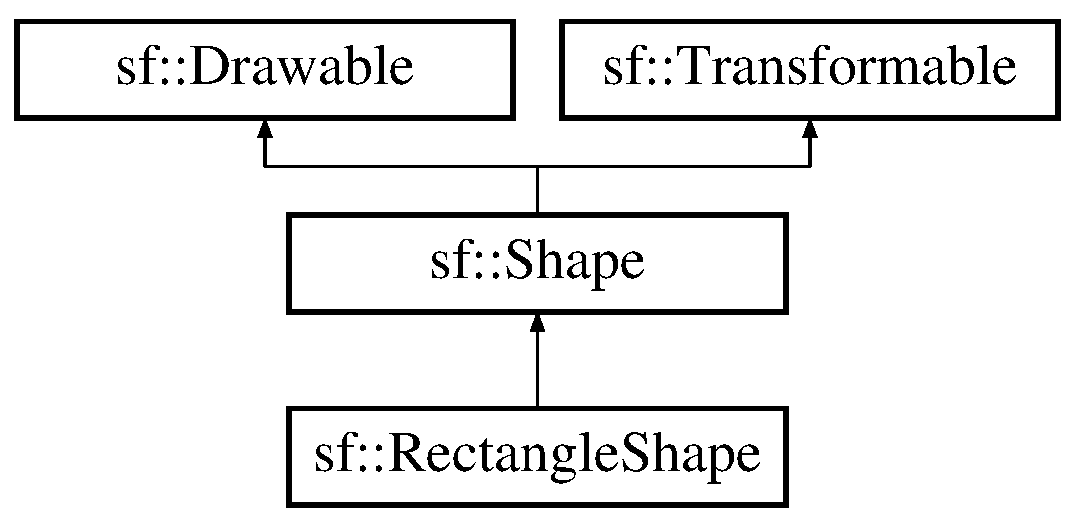
\includegraphics[height=3.000000cm]{classsf_1_1RectangleShape}
\end{center}
\end{figure}
\subsection*{Public Member Functions}
\begin{DoxyCompactItemize}
\item 
\hyperlink{classsf_1_1RectangleShape_a83a2be157ebee85c95ed491c3e78dd7c}{Rectangle\-Shape} (const \hyperlink{classsf_1_1Vector2}{Vector2f} \&size=\hyperlink{classsf_1_1Vector2}{Vector2f}(0, 0))
\begin{DoxyCompactList}\small\item\em Default constructor. \end{DoxyCompactList}\item 
void \hyperlink{classsf_1_1RectangleShape_a5c65d374d4a259dfdc24efdd24a5dbec}{set\-Size} (const \hyperlink{classsf_1_1Vector2}{Vector2f} \&size)
\begin{DoxyCompactList}\small\item\em Set the size of the rectangle. \end{DoxyCompactList}\item 
const \hyperlink{classsf_1_1Vector2}{Vector2f} \& \hyperlink{classsf_1_1RectangleShape_acaacbaee87c38a526a9d895742faab54}{get\-Size} () const 
\begin{DoxyCompactList}\small\item\em Get the size of the rectangle. \end{DoxyCompactList}\item 
virtual unsigned int \hyperlink{classsf_1_1RectangleShape_a439f5a92583baf972878c836b73bf955}{get\-Point\-Count} () const 
\begin{DoxyCompactList}\small\item\em Get the number of points defining the shape. \end{DoxyCompactList}\item 
virtual \hyperlink{classsf_1_1Vector2}{Vector2f} \hyperlink{classsf_1_1RectangleShape_a3994f7f937d6332fe64b6990d5bc43a1}{get\-Point} (unsigned int index) const 
\begin{DoxyCompactList}\small\item\em Get a point of the shape. \end{DoxyCompactList}\end{DoxyCompactItemize}
\subsection*{Additional Inherited Members}


\subsection{Detailed Description}
Specialized shape representing a rectangle. 

This class inherits all the functions of \hyperlink{classsf_1_1Transformable}{sf\-::\-Transformable} (position, rotation, scale, bounds, ...) as well as the functions of \hyperlink{classsf_1_1Shape}{sf\-::\-Shape} (outline, color, texture, ...).

Usage example\-: 
\begin{DoxyCode}
\hyperlink{classsf_1_1RectangleShape}{sf::RectangleShape} rectangle;
rectangle.\hyperlink{classsf_1_1RectangleShape_a5c65d374d4a259dfdc24efdd24a5dbec}{setSize}(\hyperlink{classsf_1_1Vector2}{sf::Vector2f}(100, 50));
rectangle.\hyperlink{classsf_1_1Shape_a5978f41ee349ac3c52942996dcb184f7}{setOutlineColor}(\hyperlink{classsf_1_1Color_a127dbf55db9c07d0fa8f4bfcbb97594a}{sf::Color::Red});
rectangle.\hyperlink{classsf_1_1Shape_a5ad336ad74fc1f567fce3b7e44cf87dc}{setOutlineThickness}(5);
rectangle.\hyperlink{classsf_1_1Transformable_a4dbfb1a7c80688b0b4c477d706550208}{setPosition}(10, 20);
...
window.draw(rectangle);
\end{DoxyCode}


\begin{DoxySeeAlso}{See Also}
\hyperlink{classsf_1_1Shape}{sf\-::\-Shape}, \hyperlink{classsf_1_1CircleShape}{sf\-::\-Circle\-Shape}, \hyperlink{classsf_1_1ConvexShape}{sf\-::\-Convex\-Shape} 
\end{DoxySeeAlso}


Definition at line 41 of file Rectangle\-Shape.\-hpp.



\subsection{Constructor \& Destructor Documentation}
\hypertarget{classsf_1_1RectangleShape_a83a2be157ebee85c95ed491c3e78dd7c}{\index{sf\-::\-Rectangle\-Shape@{sf\-::\-Rectangle\-Shape}!Rectangle\-Shape@{Rectangle\-Shape}}
\index{Rectangle\-Shape@{Rectangle\-Shape}!sf::RectangleShape@{sf\-::\-Rectangle\-Shape}}
\subsubsection[{Rectangle\-Shape}]{\setlength{\rightskip}{0pt plus 5cm}sf\-::\-Rectangle\-Shape\-::\-Rectangle\-Shape (
\begin{DoxyParamCaption}
\item[{const {\bf Vector2f} \&}]{size = {\ttfamily {\bf Vector2f}(0,~0)}}
\end{DoxyParamCaption}
)\hspace{0.3cm}{\ttfamily [explicit]}}}\label{classsf_1_1RectangleShape_a83a2be157ebee85c95ed491c3e78dd7c}


Default constructor. 


\begin{DoxyParams}{Parameters}
{\em size} & Size of the rectangle \\
\hline
\end{DoxyParams}


\subsection{Member Function Documentation}
\hypertarget{classsf_1_1RectangleShape_a3994f7f937d6332fe64b6990d5bc43a1}{\index{sf\-::\-Rectangle\-Shape@{sf\-::\-Rectangle\-Shape}!get\-Point@{get\-Point}}
\index{get\-Point@{get\-Point}!sf::RectangleShape@{sf\-::\-Rectangle\-Shape}}
\subsubsection[{get\-Point}]{\setlength{\rightskip}{0pt plus 5cm}virtual {\bf Vector2f} sf\-::\-Rectangle\-Shape\-::get\-Point (
\begin{DoxyParamCaption}
\item[{unsigned int}]{index}
\end{DoxyParamCaption}
) const\hspace{0.3cm}{\ttfamily [virtual]}}}\label{classsf_1_1RectangleShape_a3994f7f937d6332fe64b6990d5bc43a1}


Get a point of the shape. 

The result is undefined if {\itshape index} is out of the valid range.


\begin{DoxyParams}{Parameters}
{\em index} & Index of the point to get, in range \mbox{[}0 .. \hyperlink{classsf_1_1RectangleShape_a439f5a92583baf972878c836b73bf955}{get\-Point\-Count()} -\/ 1\mbox{]}\\
\hline
\end{DoxyParams}
\begin{DoxyReturn}{Returns}
Index-\/th point of the shape 
\end{DoxyReturn}


Implements \hyperlink{classsf_1_1Shape_a397f3b4cdb7ad98cdc6c034816c652d2}{sf\-::\-Shape}.

\hypertarget{classsf_1_1RectangleShape_a439f5a92583baf972878c836b73bf955}{\index{sf\-::\-Rectangle\-Shape@{sf\-::\-Rectangle\-Shape}!get\-Point\-Count@{get\-Point\-Count}}
\index{get\-Point\-Count@{get\-Point\-Count}!sf::RectangleShape@{sf\-::\-Rectangle\-Shape}}
\subsubsection[{get\-Point\-Count}]{\setlength{\rightskip}{0pt plus 5cm}virtual unsigned int sf\-::\-Rectangle\-Shape\-::get\-Point\-Count (
\begin{DoxyParamCaption}
{}
\end{DoxyParamCaption}
) const\hspace{0.3cm}{\ttfamily [virtual]}}}\label{classsf_1_1RectangleShape_a439f5a92583baf972878c836b73bf955}


Get the number of points defining the shape. 

\begin{DoxyReturn}{Returns}
Number of points of the shape 
\end{DoxyReturn}


Implements \hyperlink{classsf_1_1Shape_ad84e1b675ecd270ad8151aea4e271a78}{sf\-::\-Shape}.

\hypertarget{classsf_1_1RectangleShape_acaacbaee87c38a526a9d895742faab54}{\index{sf\-::\-Rectangle\-Shape@{sf\-::\-Rectangle\-Shape}!get\-Size@{get\-Size}}
\index{get\-Size@{get\-Size}!sf::RectangleShape@{sf\-::\-Rectangle\-Shape}}
\subsubsection[{get\-Size}]{\setlength{\rightskip}{0pt plus 5cm}const {\bf Vector2f}\& sf\-::\-Rectangle\-Shape\-::get\-Size (
\begin{DoxyParamCaption}
{}
\end{DoxyParamCaption}
) const}}\label{classsf_1_1RectangleShape_acaacbaee87c38a526a9d895742faab54}


Get the size of the rectangle. 

\begin{DoxyReturn}{Returns}
Size of the rectangle
\end{DoxyReturn}
\begin{DoxySeeAlso}{See Also}
\hyperlink{classsf_1_1RectangleShape_a5c65d374d4a259dfdc24efdd24a5dbec}{set\-Size} 
\end{DoxySeeAlso}
\hypertarget{classsf_1_1RectangleShape_a5c65d374d4a259dfdc24efdd24a5dbec}{\index{sf\-::\-Rectangle\-Shape@{sf\-::\-Rectangle\-Shape}!set\-Size@{set\-Size}}
\index{set\-Size@{set\-Size}!sf::RectangleShape@{sf\-::\-Rectangle\-Shape}}
\subsubsection[{set\-Size}]{\setlength{\rightskip}{0pt plus 5cm}void sf\-::\-Rectangle\-Shape\-::set\-Size (
\begin{DoxyParamCaption}
\item[{const {\bf Vector2f} \&}]{size}
\end{DoxyParamCaption}
)}}\label{classsf_1_1RectangleShape_a5c65d374d4a259dfdc24efdd24a5dbec}


Set the size of the rectangle. 


\begin{DoxyParams}{Parameters}
{\em size} & New size of the rectangle\\
\hline
\end{DoxyParams}
\begin{DoxySeeAlso}{See Also}
\hyperlink{classsf_1_1RectangleShape_acaacbaee87c38a526a9d895742faab54}{get\-Size} 
\end{DoxySeeAlso}


The documentation for this class was generated from the following file\-:\begin{DoxyCompactItemize}
\item 
/home/z\-Zelman/\-Dropbox/\-Placeholder-\/\-R\-T\-S/\-S\-F\-M\-L-\/2.\-1/include/\-S\-F\-M\-L/\-Graphics/Rectangle\-Shape.\-hpp\end{DoxyCompactItemize}

\hypertarget{classsf_1_1RenderStates}{\section{sf\-:\-:Render\-States Class Reference}
\label{classsf_1_1RenderStates}\index{sf\-::\-Render\-States@{sf\-::\-Render\-States}}
}


Define the states used for drawing to a \hyperlink{classsf_1_1RenderTarget}{Render\-Target}.  




{\ttfamily \#include $<$Render\-States.\-hpp$>$}

\subsection*{Public Member Functions}
\begin{DoxyCompactItemize}
\item 
\hyperlink{classsf_1_1RenderStates_a885bf14070d0d5391f062f62b270b7d0}{Render\-States} ()
\begin{DoxyCompactList}\small\item\em Default constructor. \end{DoxyCompactList}\item 
\hyperlink{classsf_1_1RenderStates_a4e3378a224f67513b95d58184e85210c}{Render\-States} (\hyperlink{group__graphics_ga80c52fe2f7050d7f7573b7ed3c995388}{Blend\-Mode} the\-Blend\-Mode)
\begin{DoxyCompactList}\small\item\em Construct a default set of render states with a custom blend mode. \end{DoxyCompactList}\item 
\hyperlink{classsf_1_1RenderStates_a3e99cad6ab05971d40357949930ed890}{Render\-States} (const \hyperlink{classsf_1_1Transform}{Transform} \&the\-Transform)
\begin{DoxyCompactList}\small\item\em Construct a default set of render states with a custom transform. \end{DoxyCompactList}\item 
\hyperlink{classsf_1_1RenderStates_a8f4ca3be0e27dafea0c4ab8547439bb1}{Render\-States} (const \hyperlink{classsf_1_1Texture}{Texture} $\ast$the\-Texture)
\begin{DoxyCompactList}\small\item\em Construct a default set of render states with a custom texture. \end{DoxyCompactList}\item 
\hyperlink{classsf_1_1RenderStates_a39f94233f464739d8d8522f3aefe97d0}{Render\-States} (const \hyperlink{classsf_1_1Shader}{Shader} $\ast$the\-Shader)
\begin{DoxyCompactList}\small\item\em Construct a default set of render states with a custom shader. \end{DoxyCompactList}\item 
\hyperlink{classsf_1_1RenderStates_ae508c91ac7b8992dc22b8d8a4027ad09}{Render\-States} (\hyperlink{group__graphics_ga80c52fe2f7050d7f7573b7ed3c995388}{Blend\-Mode} the\-Blend\-Mode, const \hyperlink{classsf_1_1Transform}{Transform} \&the\-Transform, const \hyperlink{classsf_1_1Texture}{Texture} $\ast$the\-Texture, const \hyperlink{classsf_1_1Shader}{Shader} $\ast$the\-Shader)
\begin{DoxyCompactList}\small\item\em Construct a set of render states with all its attributes. \end{DoxyCompactList}\end{DoxyCompactItemize}
\subsection*{Public Attributes}
\begin{DoxyCompactItemize}
\item 
\hypertarget{classsf_1_1RenderStates_ad6ac87f1b5006dae7ebfee4b5d40f5a8}{\hyperlink{group__graphics_ga80c52fe2f7050d7f7573b7ed3c995388}{Blend\-Mode} \hyperlink{classsf_1_1RenderStates_ad6ac87f1b5006dae7ebfee4b5d40f5a8}{blend\-Mode}}\label{classsf_1_1RenderStates_ad6ac87f1b5006dae7ebfee4b5d40f5a8}

\begin{DoxyCompactList}\small\item\em Blending mode. \end{DoxyCompactList}\item 
\hypertarget{classsf_1_1RenderStates_a1f737981a0f2f0d4bb8dac866a8d1149}{\hyperlink{classsf_1_1Transform}{Transform} \hyperlink{classsf_1_1RenderStates_a1f737981a0f2f0d4bb8dac866a8d1149}{transform}}\label{classsf_1_1RenderStates_a1f737981a0f2f0d4bb8dac866a8d1149}

\begin{DoxyCompactList}\small\item\em \hyperlink{classsf_1_1Transform}{Transform}. \end{DoxyCompactList}\item 
\hypertarget{classsf_1_1RenderStates_a457fc5a41731889de9cf39cf9b3436c3}{const \hyperlink{classsf_1_1Texture}{Texture} $\ast$ \hyperlink{classsf_1_1RenderStates_a457fc5a41731889de9cf39cf9b3436c3}{texture}}\label{classsf_1_1RenderStates_a457fc5a41731889de9cf39cf9b3436c3}

\begin{DoxyCompactList}\small\item\em \hyperlink{classsf_1_1Texture}{Texture}. \end{DoxyCompactList}\item 
\hypertarget{classsf_1_1RenderStates_ad4f79ecdd0c60ed0d24fbe555b221bd8}{const \hyperlink{classsf_1_1Shader}{Shader} $\ast$ \hyperlink{classsf_1_1RenderStates_ad4f79ecdd0c60ed0d24fbe555b221bd8}{shader}}\label{classsf_1_1RenderStates_ad4f79ecdd0c60ed0d24fbe555b221bd8}

\begin{DoxyCompactList}\small\item\em \hyperlink{classsf_1_1Shader}{Shader}. \end{DoxyCompactList}\end{DoxyCompactItemize}
\subsection*{Static Public Attributes}
\begin{DoxyCompactItemize}
\item 
\hypertarget{classsf_1_1RenderStates_ad29672df29f19ce50c3021d95f2bb062}{static const \hyperlink{classsf_1_1RenderStates}{Render\-States} \hyperlink{classsf_1_1RenderStates_ad29672df29f19ce50c3021d95f2bb062}{Default}}\label{classsf_1_1RenderStates_ad29672df29f19ce50c3021d95f2bb062}

\begin{DoxyCompactList}\small\item\em Special instance holding the default render states. \end{DoxyCompactList}\end{DoxyCompactItemize}


\subsection{Detailed Description}
Define the states used for drawing to a \hyperlink{classsf_1_1RenderTarget}{Render\-Target}. 

There are four global states that can be applied to the drawn objects\-: \begin{DoxyItemize}
\item the blend mode\-: how pixels of the object are blended with the background \item the transform\-: how the object is positioned/rotated/scaled \item the texture\-: what image is mapped to the object \item the shader\-: what custom effect is applied to the object\end{DoxyItemize}
High-\/level objects such as sprites or text force some of these states when they are drawn. For example, a sprite will set its own texture, so that you don't have to care about it when drawing the sprite.

The transform is a special case\-: sprites, texts and shapes (and it's a good idea to do it with your own drawable classes too) combine their transform with the one that is passed in the \hyperlink{classsf_1_1RenderStates}{Render\-States} structure. So that you can use a \char`\"{}global\char`\"{} transform on top of each object's transform.

Most objects, especially high-\/level drawables, can be drawn directly without defining render states explicitely -- the default set of states is ok in most cases. 
\begin{DoxyCode}
window.Draw(sprite);
\end{DoxyCode}


If you want to use a single specific render state, for example a shader, you can pass it directly to the Draw function\-: \hyperlink{classsf_1_1RenderStates}{sf\-::\-Render\-States} has an implicit one-\/argument constructor for each state. 
\begin{DoxyCode}
window.draw(sprite, \hyperlink{classsf_1_1RenderStates_ad4f79ecdd0c60ed0d24fbe555b221bd8}{shader});
\end{DoxyCode}


When you're inside the Draw function of a drawable object (inherited from \hyperlink{classsf_1_1Drawable}{sf\-::\-Drawable}), you can either pass the render states unmodified, or change some of them. For example, a transformable object will combine the current transform with its own transform. A sprite will set its texture. Etc.

\begin{DoxySeeAlso}{See Also}
\hyperlink{classsf_1_1RenderTarget}{sf\-::\-Render\-Target}, \hyperlink{classsf_1_1Drawable}{sf\-::\-Drawable} 
\end{DoxySeeAlso}


Definition at line 45 of file Render\-States.\-hpp.



\subsection{Constructor \& Destructor Documentation}
\hypertarget{classsf_1_1RenderStates_a885bf14070d0d5391f062f62b270b7d0}{\index{sf\-::\-Render\-States@{sf\-::\-Render\-States}!Render\-States@{Render\-States}}
\index{Render\-States@{Render\-States}!sf::RenderStates@{sf\-::\-Render\-States}}
\subsubsection[{Render\-States}]{\setlength{\rightskip}{0pt plus 5cm}sf\-::\-Render\-States\-::\-Render\-States (
\begin{DoxyParamCaption}
{}
\end{DoxyParamCaption}
)}}\label{classsf_1_1RenderStates_a885bf14070d0d5391f062f62b270b7d0}


Default constructor. 

Constructing a default set of render states is equivalent to using \hyperlink{classsf_1_1RenderStates_ad29672df29f19ce50c3021d95f2bb062}{sf\-::\-Render\-States\-::\-Default}. The default set defines\-: \begin{DoxyItemize}
\item the Blend\-Alpha blend mode \item the identity transform \item a null texture \item a null shader \end{DoxyItemize}
\hypertarget{classsf_1_1RenderStates_a4e3378a224f67513b95d58184e85210c}{\index{sf\-::\-Render\-States@{sf\-::\-Render\-States}!Render\-States@{Render\-States}}
\index{Render\-States@{Render\-States}!sf::RenderStates@{sf\-::\-Render\-States}}
\subsubsection[{Render\-States}]{\setlength{\rightskip}{0pt plus 5cm}sf\-::\-Render\-States\-::\-Render\-States (
\begin{DoxyParamCaption}
\item[{{\bf Blend\-Mode}}]{the\-Blend\-Mode}
\end{DoxyParamCaption}
)}}\label{classsf_1_1RenderStates_a4e3378a224f67513b95d58184e85210c}


Construct a default set of render states with a custom blend mode. 


\begin{DoxyParams}{Parameters}
{\em the\-Blend\-Mode} & Blend mode to use \\
\hline
\end{DoxyParams}
\hypertarget{classsf_1_1RenderStates_a3e99cad6ab05971d40357949930ed890}{\index{sf\-::\-Render\-States@{sf\-::\-Render\-States}!Render\-States@{Render\-States}}
\index{Render\-States@{Render\-States}!sf::RenderStates@{sf\-::\-Render\-States}}
\subsubsection[{Render\-States}]{\setlength{\rightskip}{0pt plus 5cm}sf\-::\-Render\-States\-::\-Render\-States (
\begin{DoxyParamCaption}
\item[{const {\bf Transform} \&}]{the\-Transform}
\end{DoxyParamCaption}
)}}\label{classsf_1_1RenderStates_a3e99cad6ab05971d40357949930ed890}


Construct a default set of render states with a custom transform. 


\begin{DoxyParams}{Parameters}
{\em the\-Transform} & \hyperlink{classsf_1_1Transform}{Transform} to use \\
\hline
\end{DoxyParams}
\hypertarget{classsf_1_1RenderStates_a8f4ca3be0e27dafea0c4ab8547439bb1}{\index{sf\-::\-Render\-States@{sf\-::\-Render\-States}!Render\-States@{Render\-States}}
\index{Render\-States@{Render\-States}!sf::RenderStates@{sf\-::\-Render\-States}}
\subsubsection[{Render\-States}]{\setlength{\rightskip}{0pt plus 5cm}sf\-::\-Render\-States\-::\-Render\-States (
\begin{DoxyParamCaption}
\item[{const {\bf Texture} $\ast$}]{the\-Texture}
\end{DoxyParamCaption}
)}}\label{classsf_1_1RenderStates_a8f4ca3be0e27dafea0c4ab8547439bb1}


Construct a default set of render states with a custom texture. 


\begin{DoxyParams}{Parameters}
{\em the\-Texture} & \hyperlink{classsf_1_1Texture}{Texture} to use \\
\hline
\end{DoxyParams}
\hypertarget{classsf_1_1RenderStates_a39f94233f464739d8d8522f3aefe97d0}{\index{sf\-::\-Render\-States@{sf\-::\-Render\-States}!Render\-States@{Render\-States}}
\index{Render\-States@{Render\-States}!sf::RenderStates@{sf\-::\-Render\-States}}
\subsubsection[{Render\-States}]{\setlength{\rightskip}{0pt plus 5cm}sf\-::\-Render\-States\-::\-Render\-States (
\begin{DoxyParamCaption}
\item[{const {\bf Shader} $\ast$}]{the\-Shader}
\end{DoxyParamCaption}
)}}\label{classsf_1_1RenderStates_a39f94233f464739d8d8522f3aefe97d0}


Construct a default set of render states with a custom shader. 


\begin{DoxyParams}{Parameters}
{\em the\-Shader} & \hyperlink{classsf_1_1Shader}{Shader} to use \\
\hline
\end{DoxyParams}
\hypertarget{classsf_1_1RenderStates_ae508c91ac7b8992dc22b8d8a4027ad09}{\index{sf\-::\-Render\-States@{sf\-::\-Render\-States}!Render\-States@{Render\-States}}
\index{Render\-States@{Render\-States}!sf::RenderStates@{sf\-::\-Render\-States}}
\subsubsection[{Render\-States}]{\setlength{\rightskip}{0pt plus 5cm}sf\-::\-Render\-States\-::\-Render\-States (
\begin{DoxyParamCaption}
\item[{{\bf Blend\-Mode}}]{the\-Blend\-Mode, }
\item[{const {\bf Transform} \&}]{the\-Transform, }
\item[{const {\bf Texture} $\ast$}]{the\-Texture, }
\item[{const {\bf Shader} $\ast$}]{the\-Shader}
\end{DoxyParamCaption}
)}}\label{classsf_1_1RenderStates_ae508c91ac7b8992dc22b8d8a4027ad09}


Construct a set of render states with all its attributes. 


\begin{DoxyParams}{Parameters}
{\em the\-Blend\-Mode} & Blend mode to use \\
\hline
{\em the\-Transform} & \hyperlink{classsf_1_1Transform}{Transform} to use \\
\hline
{\em the\-Texture} & \hyperlink{classsf_1_1Texture}{Texture} to use \\
\hline
{\em the\-Shader} & \hyperlink{classsf_1_1Shader}{Shader} to use \\
\hline
\end{DoxyParams}


The documentation for this class was generated from the following file\-:\begin{DoxyCompactItemize}
\item 
/home/z\-Zelman/\-Dropbox/\-Placeholder-\/\-R\-T\-S/\-S\-F\-M\-L-\/2.\-1/include/\-S\-F\-M\-L/\-Graphics/Render\-States.\-hpp\end{DoxyCompactItemize}

\hypertarget{classsf_1_1RenderTarget}{\section{sf\-:\-:Render\-Target Class Reference}
\label{classsf_1_1RenderTarget}\index{sf\-::\-Render\-Target@{sf\-::\-Render\-Target}}
}


Base class for all render targets (window, texture, ...)  




{\ttfamily \#include $<$Render\-Target.\-hpp$>$}

Inheritance diagram for sf\-:\-:Render\-Target\-:\begin{figure}[H]
\begin{center}
\leavevmode
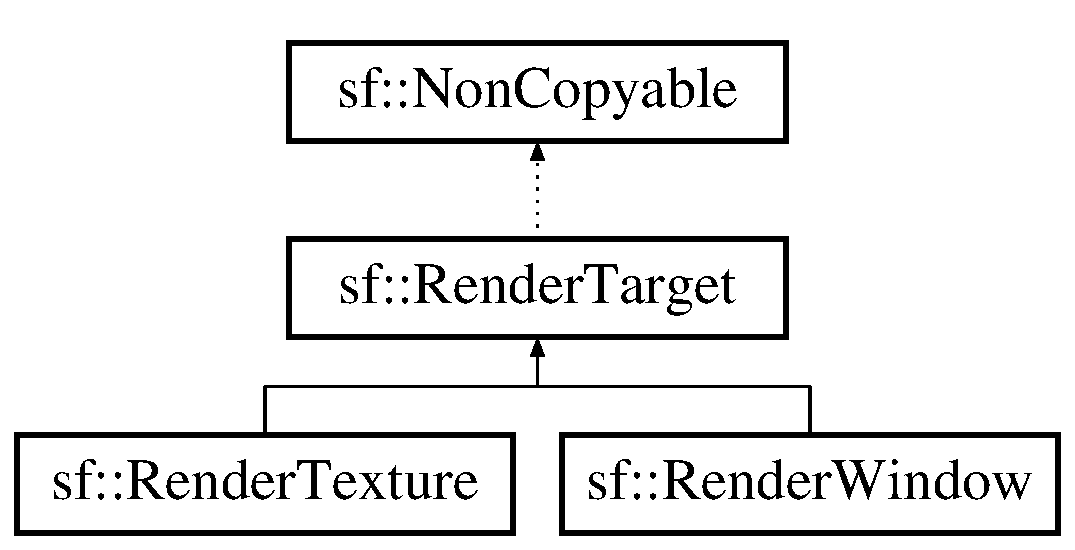
\includegraphics[height=3.000000cm]{classsf_1_1RenderTarget}
\end{center}
\end{figure}
\subsection*{Public Member Functions}
\begin{DoxyCompactItemize}
\item 
\hypertarget{classsf_1_1RenderTarget_a9abd1654a99fba46f6887b9c625b9b06}{virtual \hyperlink{classsf_1_1RenderTarget_a9abd1654a99fba46f6887b9c625b9b06}{$\sim$\-Render\-Target} ()}\label{classsf_1_1RenderTarget_a9abd1654a99fba46f6887b9c625b9b06}

\begin{DoxyCompactList}\small\item\em Destructor. \end{DoxyCompactList}\item 
void \hyperlink{classsf_1_1RenderTarget_a6bb6f0ba348f2b1e2f46114aeaf60f26}{clear} (const \hyperlink{classsf_1_1Color}{Color} \&color=\hyperlink{classsf_1_1Color}{Color}(0, 0, 0, 255))
\begin{DoxyCompactList}\small\item\em Clear the entire target with a single color. \end{DoxyCompactList}\item 
void \hyperlink{classsf_1_1RenderTarget_a063db6dd0a14913504af30e50cb6d946}{set\-View} (const \hyperlink{classsf_1_1View}{View} \&view)
\begin{DoxyCompactList}\small\item\em Change the current active view. \end{DoxyCompactList}\item 
const \hyperlink{classsf_1_1View}{View} \& \hyperlink{classsf_1_1RenderTarget_a98f721cc6dc11478922427fedfb2288b}{get\-View} () const 
\begin{DoxyCompactList}\small\item\em Get the view currently in use in the render target. \end{DoxyCompactList}\item 
const \hyperlink{classsf_1_1View}{View} \& \hyperlink{classsf_1_1RenderTarget_a718b1aa6296bf855171699cc18251ced}{get\-Default\-View} () const 
\begin{DoxyCompactList}\small\item\em Get the default view of the render target. \end{DoxyCompactList}\item 
\hyperlink{classsf_1_1Rect}{Int\-Rect} \hyperlink{classsf_1_1RenderTarget_aae035b0d45f87a0da2a28a0de6ba1086}{get\-Viewport} (const \hyperlink{classsf_1_1View}{View} \&view) const 
\begin{DoxyCompactList}\small\item\em Get the viewport of a view, applied to this render target. \end{DoxyCompactList}\item 
\hyperlink{classsf_1_1Vector2}{Vector2f} \hyperlink{classsf_1_1RenderTarget_a2b0cab0e4c6af29d4efaba149d28116d}{map\-Pixel\-To\-Coords} (const \hyperlink{classsf_1_1Vector2}{Vector2i} \&point) const 
\begin{DoxyCompactList}\small\item\em Convert a point from target coordinates to world coordinates, using the current view. \end{DoxyCompactList}\item 
\hyperlink{classsf_1_1Vector2}{Vector2f} \hyperlink{classsf_1_1RenderTarget_a46eb08f775dd1420d6207ea87dde6e54}{map\-Pixel\-To\-Coords} (const \hyperlink{classsf_1_1Vector2}{Vector2i} \&point, const \hyperlink{classsf_1_1View}{View} \&view) const 
\begin{DoxyCompactList}\small\item\em Convert a point from target coordinates to world coordinates. \end{DoxyCompactList}\item 
\hyperlink{classsf_1_1Vector2}{Vector2i} \hyperlink{classsf_1_1RenderTarget_aa0c11e1989573f2cce64c621205f8e83}{map\-Coords\-To\-Pixel} (const \hyperlink{classsf_1_1Vector2}{Vector2f} \&point) const 
\begin{DoxyCompactList}\small\item\em Convert a point from world coordinates to target coordinates, using the current view. \end{DoxyCompactList}\item 
\hyperlink{classsf_1_1Vector2}{Vector2i} \hyperlink{classsf_1_1RenderTarget_a7a2d427bdb9bd8f9f456fcf82813aa60}{map\-Coords\-To\-Pixel} (const \hyperlink{classsf_1_1Vector2}{Vector2f} \&point, const \hyperlink{classsf_1_1View}{View} \&view) const 
\begin{DoxyCompactList}\small\item\em Convert a point from world coordinates to target coordinates. \end{DoxyCompactList}\item 
void \hyperlink{classsf_1_1RenderTarget_a12417a3bcc245c41d957b29583556f39}{draw} (const \hyperlink{classsf_1_1Drawable}{Drawable} \&drawable, const \hyperlink{classsf_1_1RenderStates}{Render\-States} \&states=\hyperlink{classsf_1_1RenderStates_ad29672df29f19ce50c3021d95f2bb062}{Render\-States\-::\-Default})
\begin{DoxyCompactList}\small\item\em Draw a drawable object to the render-\/target. \end{DoxyCompactList}\item 
void \hyperlink{classsf_1_1RenderTarget_ab636d7363f6681077361ee274ba89a8d}{draw} (const \hyperlink{classsf_1_1Vertex}{Vertex} $\ast$vertices, unsigned int vertex\-Count, \hyperlink{group__graphics_ga5ee56ac1339984909610713096283b1b}{Primitive\-Type} type, const \hyperlink{classsf_1_1RenderStates}{Render\-States} \&states=\hyperlink{classsf_1_1RenderStates_ad29672df29f19ce50c3021d95f2bb062}{Render\-States\-::\-Default})
\begin{DoxyCompactList}\small\item\em Draw primitives defined by an array of vertices. \end{DoxyCompactList}\item 
virtual \hyperlink{classsf_1_1Vector2}{Vector2u} \hyperlink{classsf_1_1RenderTarget_a2e5ade2457d9fb4c4907ae5b3d9e94a5}{get\-Size} () const =0
\begin{DoxyCompactList}\small\item\em Return the size of the rendering region of the target. \end{DoxyCompactList}\item 
void \hyperlink{classsf_1_1RenderTarget_a8d1998464ccc54e789aaf990242b47f7}{push\-G\-L\-States} ()
\begin{DoxyCompactList}\small\item\em Save the current Open\-G\-L render states and matrices. \end{DoxyCompactList}\item 
void \hyperlink{classsf_1_1RenderTarget_ad5a98401113df931ddcd54c080f7aa8e}{pop\-G\-L\-States} ()
\begin{DoxyCompactList}\small\item\em Restore the previously saved Open\-G\-L render states and matrices. \end{DoxyCompactList}\item 
void \hyperlink{classsf_1_1RenderTarget_aac7504990d27dada4bfe3c7866920765}{reset\-G\-L\-States} ()
\begin{DoxyCompactList}\small\item\em Reset the internal Open\-G\-L states so that the target is ready for drawing. \end{DoxyCompactList}\end{DoxyCompactItemize}
\subsection*{Protected Member Functions}
\begin{DoxyCompactItemize}
\item 
\hypertarget{classsf_1_1RenderTarget_a2997c96cbd93cb8ce0aba2ddae35b86f}{\hyperlink{classsf_1_1RenderTarget_a2997c96cbd93cb8ce0aba2ddae35b86f}{Render\-Target} ()}\label{classsf_1_1RenderTarget_a2997c96cbd93cb8ce0aba2ddae35b86f}

\begin{DoxyCompactList}\small\item\em Default constructor. \end{DoxyCompactList}\item 
void \hyperlink{classsf_1_1RenderTarget_af530274b34159d644e509b4b4dc43eb7}{initialize} ()
\begin{DoxyCompactList}\small\item\em Performs the common initialization step after creation. \end{DoxyCompactList}\end{DoxyCompactItemize}


\subsection{Detailed Description}
Base class for all render targets (window, texture, ...) 

\hyperlink{classsf_1_1RenderTarget}{sf\-::\-Render\-Target} defines the common behaviour of all the 2\-D render targets usable in the graphics module. It makes it possible to draw 2\-D entities like sprites, shapes, text without using any Open\-G\-L command directly.

A \hyperlink{classsf_1_1RenderTarget}{sf\-::\-Render\-Target} is also able to use views (\hyperlink{classsf_1_1View}{sf\-::\-View}), which are a kind of 2\-D cameras. With views you can globally scroll, rotate or zoom everything that is drawn, without having to transform every single entity. See the documentation of \hyperlink{classsf_1_1View}{sf\-::\-View} for more details and sample pieces of code about this class.

On top of that, render targets are still able to render direct Open\-G\-L stuff. It is even possible to mix together Open\-G\-L calls and regular S\-F\-M\-L drawing commands. When doing so, make sure that Open\-G\-L states are not messed up by calling the push\-G\-L\-States/pop\-G\-L\-States functions.

\begin{DoxySeeAlso}{See Also}
\hyperlink{classsf_1_1RenderWindow}{sf\-::\-Render\-Window}, \hyperlink{classsf_1_1RenderTexture}{sf\-::\-Render\-Texture}, \hyperlink{classsf_1_1View}{sf\-::\-View} 
\end{DoxySeeAlso}


Definition at line 51 of file Render\-Target.\-hpp.



\subsection{Member Function Documentation}
\hypertarget{classsf_1_1RenderTarget_a6bb6f0ba348f2b1e2f46114aeaf60f26}{\index{sf\-::\-Render\-Target@{sf\-::\-Render\-Target}!clear@{clear}}
\index{clear@{clear}!sf::RenderTarget@{sf\-::\-Render\-Target}}
\subsubsection[{clear}]{\setlength{\rightskip}{0pt plus 5cm}void sf\-::\-Render\-Target\-::clear (
\begin{DoxyParamCaption}
\item[{const {\bf Color} \&}]{color = {\ttfamily {\bf Color}(0,~0,~0,~255)}}
\end{DoxyParamCaption}
)}}\label{classsf_1_1RenderTarget_a6bb6f0ba348f2b1e2f46114aeaf60f26}


Clear the entire target with a single color. 

This function is usually called once every frame, to clear the previous contents of the target.


\begin{DoxyParams}{Parameters}
{\em color} & Fill color to use to clear the render target \\
\hline
\end{DoxyParams}
\hypertarget{classsf_1_1RenderTarget_a12417a3bcc245c41d957b29583556f39}{\index{sf\-::\-Render\-Target@{sf\-::\-Render\-Target}!draw@{draw}}
\index{draw@{draw}!sf::RenderTarget@{sf\-::\-Render\-Target}}
\subsubsection[{draw}]{\setlength{\rightskip}{0pt plus 5cm}void sf\-::\-Render\-Target\-::draw (
\begin{DoxyParamCaption}
\item[{const {\bf Drawable} \&}]{drawable, }
\item[{const {\bf Render\-States} \&}]{states = {\ttfamily {\bf Render\-States\-::\-Default}}}
\end{DoxyParamCaption}
)}}\label{classsf_1_1RenderTarget_a12417a3bcc245c41d957b29583556f39}


Draw a drawable object to the render-\/target. 


\begin{DoxyParams}{Parameters}
{\em drawable} & Object to draw \\
\hline
{\em states} & Render states to use for drawing \\
\hline
\end{DoxyParams}
\hypertarget{classsf_1_1RenderTarget_ab636d7363f6681077361ee274ba89a8d}{\index{sf\-::\-Render\-Target@{sf\-::\-Render\-Target}!draw@{draw}}
\index{draw@{draw}!sf::RenderTarget@{sf\-::\-Render\-Target}}
\subsubsection[{draw}]{\setlength{\rightskip}{0pt plus 5cm}void sf\-::\-Render\-Target\-::draw (
\begin{DoxyParamCaption}
\item[{const {\bf Vertex} $\ast$}]{vertices, }
\item[{unsigned int}]{vertex\-Count, }
\item[{{\bf Primitive\-Type}}]{type, }
\item[{const {\bf Render\-States} \&}]{states = {\ttfamily {\bf Render\-States\-::\-Default}}}
\end{DoxyParamCaption}
)}}\label{classsf_1_1RenderTarget_ab636d7363f6681077361ee274ba89a8d}


Draw primitives defined by an array of vertices. 


\begin{DoxyParams}{Parameters}
{\em vertices} & Pointer to the vertices \\
\hline
{\em vertex\-Count} & Number of vertices in the array \\
\hline
{\em type} & Type of primitives to draw \\
\hline
{\em states} & Render states to use for drawing \\
\hline
\end{DoxyParams}
\hypertarget{classsf_1_1RenderTarget_a718b1aa6296bf855171699cc18251ced}{\index{sf\-::\-Render\-Target@{sf\-::\-Render\-Target}!get\-Default\-View@{get\-Default\-View}}
\index{get\-Default\-View@{get\-Default\-View}!sf::RenderTarget@{sf\-::\-Render\-Target}}
\subsubsection[{get\-Default\-View}]{\setlength{\rightskip}{0pt plus 5cm}const {\bf View}\& sf\-::\-Render\-Target\-::get\-Default\-View (
\begin{DoxyParamCaption}
{}
\end{DoxyParamCaption}
) const}}\label{classsf_1_1RenderTarget_a718b1aa6296bf855171699cc18251ced}


Get the default view of the render target. 

The default view has the initial size of the render target, and never changes after the target has been created.

\begin{DoxyReturn}{Returns}
The default view of the render target
\end{DoxyReturn}
\begin{DoxySeeAlso}{See Also}
\hyperlink{classsf_1_1RenderTarget_a063db6dd0a14913504af30e50cb6d946}{set\-View}, \hyperlink{classsf_1_1RenderTarget_a98f721cc6dc11478922427fedfb2288b}{get\-View} 
\end{DoxySeeAlso}
\hypertarget{classsf_1_1RenderTarget_a2e5ade2457d9fb4c4907ae5b3d9e94a5}{\index{sf\-::\-Render\-Target@{sf\-::\-Render\-Target}!get\-Size@{get\-Size}}
\index{get\-Size@{get\-Size}!sf::RenderTarget@{sf\-::\-Render\-Target}}
\subsubsection[{get\-Size}]{\setlength{\rightskip}{0pt plus 5cm}virtual {\bf Vector2u} sf\-::\-Render\-Target\-::get\-Size (
\begin{DoxyParamCaption}
{}
\end{DoxyParamCaption}
) const\hspace{0.3cm}{\ttfamily [pure virtual]}}}\label{classsf_1_1RenderTarget_a2e5ade2457d9fb4c4907ae5b3d9e94a5}


Return the size of the rendering region of the target. 

\begin{DoxyReturn}{Returns}
Size in pixels 
\end{DoxyReturn}


Implemented in \hyperlink{classsf_1_1RenderTexture_a757ba45ec7a7deefcaef717049b00b8c}{sf\-::\-Render\-Texture}, and \hyperlink{classsf_1_1RenderWindow_a2c7ff414be32621a453745cf2a0f8a3e}{sf\-::\-Render\-Window}.

\hypertarget{classsf_1_1RenderTarget_a98f721cc6dc11478922427fedfb2288b}{\index{sf\-::\-Render\-Target@{sf\-::\-Render\-Target}!get\-View@{get\-View}}
\index{get\-View@{get\-View}!sf::RenderTarget@{sf\-::\-Render\-Target}}
\subsubsection[{get\-View}]{\setlength{\rightskip}{0pt plus 5cm}const {\bf View}\& sf\-::\-Render\-Target\-::get\-View (
\begin{DoxyParamCaption}
{}
\end{DoxyParamCaption}
) const}}\label{classsf_1_1RenderTarget_a98f721cc6dc11478922427fedfb2288b}


Get the view currently in use in the render target. 

\begin{DoxyReturn}{Returns}
The view object that is currently used
\end{DoxyReturn}
\begin{DoxySeeAlso}{See Also}
\hyperlink{classsf_1_1RenderTarget_a063db6dd0a14913504af30e50cb6d946}{set\-View}, \hyperlink{classsf_1_1RenderTarget_a718b1aa6296bf855171699cc18251ced}{get\-Default\-View} 
\end{DoxySeeAlso}
\hypertarget{classsf_1_1RenderTarget_aae035b0d45f87a0da2a28a0de6ba1086}{\index{sf\-::\-Render\-Target@{sf\-::\-Render\-Target}!get\-Viewport@{get\-Viewport}}
\index{get\-Viewport@{get\-Viewport}!sf::RenderTarget@{sf\-::\-Render\-Target}}
\subsubsection[{get\-Viewport}]{\setlength{\rightskip}{0pt plus 5cm}{\bf Int\-Rect} sf\-::\-Render\-Target\-::get\-Viewport (
\begin{DoxyParamCaption}
\item[{const {\bf View} \&}]{view}
\end{DoxyParamCaption}
) const}}\label{classsf_1_1RenderTarget_aae035b0d45f87a0da2a28a0de6ba1086}


Get the viewport of a view, applied to this render target. 

The viewport is defined in the view as a ratio, this function simply applies this ratio to the current dimensions of the render target to calculate the pixels rectangle that the viewport actually covers in the target.


\begin{DoxyParams}{Parameters}
{\em view} & The view for which we want to compute the viewport\\
\hline
\end{DoxyParams}
\begin{DoxyReturn}{Returns}
Viewport rectangle, expressed in pixels 
\end{DoxyReturn}
\hypertarget{classsf_1_1RenderTarget_af530274b34159d644e509b4b4dc43eb7}{\index{sf\-::\-Render\-Target@{sf\-::\-Render\-Target}!initialize@{initialize}}
\index{initialize@{initialize}!sf::RenderTarget@{sf\-::\-Render\-Target}}
\subsubsection[{initialize}]{\setlength{\rightskip}{0pt plus 5cm}void sf\-::\-Render\-Target\-::initialize (
\begin{DoxyParamCaption}
{}
\end{DoxyParamCaption}
)\hspace{0.3cm}{\ttfamily [protected]}}}\label{classsf_1_1RenderTarget_af530274b34159d644e509b4b4dc43eb7}


Performs the common initialization step after creation. 

The derived classes must call this function after the target is created and ready for drawing. \hypertarget{classsf_1_1RenderTarget_aa0c11e1989573f2cce64c621205f8e83}{\index{sf\-::\-Render\-Target@{sf\-::\-Render\-Target}!map\-Coords\-To\-Pixel@{map\-Coords\-To\-Pixel}}
\index{map\-Coords\-To\-Pixel@{map\-Coords\-To\-Pixel}!sf::RenderTarget@{sf\-::\-Render\-Target}}
\subsubsection[{map\-Coords\-To\-Pixel}]{\setlength{\rightskip}{0pt plus 5cm}{\bf Vector2i} sf\-::\-Render\-Target\-::map\-Coords\-To\-Pixel (
\begin{DoxyParamCaption}
\item[{const {\bf Vector2f} \&}]{point}
\end{DoxyParamCaption}
) const}}\label{classsf_1_1RenderTarget_aa0c11e1989573f2cce64c621205f8e83}


Convert a point from world coordinates to target coordinates, using the current view. 

This function is an overload of the map\-Coords\-To\-Pixel function that implicitely uses the current view. It is equivalent to\-: 
\begin{DoxyCode}
target.\hyperlink{classsf_1_1RenderTarget_aa0c11e1989573f2cce64c621205f8e83}{mapCoordsToPixel}(point, target.\hyperlink{classsf_1_1RenderTarget_a98f721cc6dc11478922427fedfb2288b}{getView}());
\end{DoxyCode}



\begin{DoxyParams}{Parameters}
{\em point} & Point to convert\\
\hline
\end{DoxyParams}
\begin{DoxyReturn}{Returns}
The converted point, in target coordinates (pixels)
\end{DoxyReturn}
\begin{DoxySeeAlso}{See Also}
\hyperlink{classsf_1_1RenderTarget_a2b0cab0e4c6af29d4efaba149d28116d}{map\-Pixel\-To\-Coords} 
\end{DoxySeeAlso}
\hypertarget{classsf_1_1RenderTarget_a7a2d427bdb9bd8f9f456fcf82813aa60}{\index{sf\-::\-Render\-Target@{sf\-::\-Render\-Target}!map\-Coords\-To\-Pixel@{map\-Coords\-To\-Pixel}}
\index{map\-Coords\-To\-Pixel@{map\-Coords\-To\-Pixel}!sf::RenderTarget@{sf\-::\-Render\-Target}}
\subsubsection[{map\-Coords\-To\-Pixel}]{\setlength{\rightskip}{0pt plus 5cm}{\bf Vector2i} sf\-::\-Render\-Target\-::map\-Coords\-To\-Pixel (
\begin{DoxyParamCaption}
\item[{const {\bf Vector2f} \&}]{point, }
\item[{const {\bf View} \&}]{view}
\end{DoxyParamCaption}
) const}}\label{classsf_1_1RenderTarget_a7a2d427bdb9bd8f9f456fcf82813aa60}


Convert a point from world coordinates to target coordinates. 

This function finds the pixel of the render-\/target that matches the given 2\-D point. In other words, it goes through the same process as the graphics card, to compute the final position of a rendered point.

Initially, both coordinate systems (world units and target pixels) match perfectly. But if you define a custom view or resize your render-\/target, this assertion is not true anymore, ie. a point located at (150, 75) in your 2\-D world may map to the pixel (10, 50) of your render-\/target -- if the view is translated by (140, 25).

This version uses a custom view for calculations, see the other overload of the function if you want to use the current view of the render-\/target.


\begin{DoxyParams}{Parameters}
{\em point} & Point to convert \\
\hline
{\em view} & The view to use for converting the point\\
\hline
\end{DoxyParams}
\begin{DoxyReturn}{Returns}
The converted point, in target coordinates (pixels)
\end{DoxyReturn}
\begin{DoxySeeAlso}{See Also}
\hyperlink{classsf_1_1RenderTarget_a2b0cab0e4c6af29d4efaba149d28116d}{map\-Pixel\-To\-Coords} 
\end{DoxySeeAlso}
\hypertarget{classsf_1_1RenderTarget_a2b0cab0e4c6af29d4efaba149d28116d}{\index{sf\-::\-Render\-Target@{sf\-::\-Render\-Target}!map\-Pixel\-To\-Coords@{map\-Pixel\-To\-Coords}}
\index{map\-Pixel\-To\-Coords@{map\-Pixel\-To\-Coords}!sf::RenderTarget@{sf\-::\-Render\-Target}}
\subsubsection[{map\-Pixel\-To\-Coords}]{\setlength{\rightskip}{0pt plus 5cm}{\bf Vector2f} sf\-::\-Render\-Target\-::map\-Pixel\-To\-Coords (
\begin{DoxyParamCaption}
\item[{const {\bf Vector2i} \&}]{point}
\end{DoxyParamCaption}
) const}}\label{classsf_1_1RenderTarget_a2b0cab0e4c6af29d4efaba149d28116d}


Convert a point from target coordinates to world coordinates, using the current view. 

This function is an overload of the map\-Pixel\-To\-Coords function that implicitely uses the current view. It is equivalent to\-: 
\begin{DoxyCode}
target.\hyperlink{classsf_1_1RenderTarget_a2b0cab0e4c6af29d4efaba149d28116d}{mapPixelToCoords}(point, target.\hyperlink{classsf_1_1RenderTarget_a98f721cc6dc11478922427fedfb2288b}{getView}());
\end{DoxyCode}



\begin{DoxyParams}{Parameters}
{\em point} & Pixel to convert\\
\hline
\end{DoxyParams}
\begin{DoxyReturn}{Returns}
The converted point, in \char`\"{}world\char`\"{} coordinates
\end{DoxyReturn}
\begin{DoxySeeAlso}{See Also}
\hyperlink{classsf_1_1RenderTarget_aa0c11e1989573f2cce64c621205f8e83}{map\-Coords\-To\-Pixel} 
\end{DoxySeeAlso}
\hypertarget{classsf_1_1RenderTarget_a46eb08f775dd1420d6207ea87dde6e54}{\index{sf\-::\-Render\-Target@{sf\-::\-Render\-Target}!map\-Pixel\-To\-Coords@{map\-Pixel\-To\-Coords}}
\index{map\-Pixel\-To\-Coords@{map\-Pixel\-To\-Coords}!sf::RenderTarget@{sf\-::\-Render\-Target}}
\subsubsection[{map\-Pixel\-To\-Coords}]{\setlength{\rightskip}{0pt plus 5cm}{\bf Vector2f} sf\-::\-Render\-Target\-::map\-Pixel\-To\-Coords (
\begin{DoxyParamCaption}
\item[{const {\bf Vector2i} \&}]{point, }
\item[{const {\bf View} \&}]{view}
\end{DoxyParamCaption}
) const}}\label{classsf_1_1RenderTarget_a46eb08f775dd1420d6207ea87dde6e54}


Convert a point from target coordinates to world coordinates. 

This function finds the 2\-D position that matches the given pixel of the render-\/target. In other words, it does the inverse of what the graphics card does, to find the initial position of a rendered pixel.

Initially, both coordinate systems (world units and target pixels) match perfectly. But if you define a custom view or resize your render-\/target, this assertion is not true anymore, ie. a point located at (10, 50) in your render-\/target may map to the point (150, 75) in your 2\-D world -- if the view is translated by (140, 25).

For render-\/windows, this function is typically used to find which point (or object) is located below the mouse cursor.

This version uses a custom view for calculations, see the other overload of the function if you want to use the current view of the render-\/target.


\begin{DoxyParams}{Parameters}
{\em point} & Pixel to convert \\
\hline
{\em view} & The view to use for converting the point\\
\hline
\end{DoxyParams}
\begin{DoxyReturn}{Returns}
The converted point, in \char`\"{}world\char`\"{} units
\end{DoxyReturn}
\begin{DoxySeeAlso}{See Also}
\hyperlink{classsf_1_1RenderTarget_aa0c11e1989573f2cce64c621205f8e83}{map\-Coords\-To\-Pixel} 
\end{DoxySeeAlso}
\hypertarget{classsf_1_1RenderTarget_ad5a98401113df931ddcd54c080f7aa8e}{\index{sf\-::\-Render\-Target@{sf\-::\-Render\-Target}!pop\-G\-L\-States@{pop\-G\-L\-States}}
\index{pop\-G\-L\-States@{pop\-G\-L\-States}!sf::RenderTarget@{sf\-::\-Render\-Target}}
\subsubsection[{pop\-G\-L\-States}]{\setlength{\rightskip}{0pt plus 5cm}void sf\-::\-Render\-Target\-::pop\-G\-L\-States (
\begin{DoxyParamCaption}
{}
\end{DoxyParamCaption}
)}}\label{classsf_1_1RenderTarget_ad5a98401113df931ddcd54c080f7aa8e}


Restore the previously saved Open\-G\-L render states and matrices. 

See the description of push\-G\-L\-States to get a detailed description of these functions.

\begin{DoxySeeAlso}{See Also}
\hyperlink{classsf_1_1RenderTarget_a8d1998464ccc54e789aaf990242b47f7}{push\-G\-L\-States} 
\end{DoxySeeAlso}
\hypertarget{classsf_1_1RenderTarget_a8d1998464ccc54e789aaf990242b47f7}{\index{sf\-::\-Render\-Target@{sf\-::\-Render\-Target}!push\-G\-L\-States@{push\-G\-L\-States}}
\index{push\-G\-L\-States@{push\-G\-L\-States}!sf::RenderTarget@{sf\-::\-Render\-Target}}
\subsubsection[{push\-G\-L\-States}]{\setlength{\rightskip}{0pt plus 5cm}void sf\-::\-Render\-Target\-::push\-G\-L\-States (
\begin{DoxyParamCaption}
{}
\end{DoxyParamCaption}
)}}\label{classsf_1_1RenderTarget_a8d1998464ccc54e789aaf990242b47f7}


Save the current Open\-G\-L render states and matrices. 

This function can be used when you mix S\-F\-M\-L drawing and direct Open\-G\-L rendering. Combined with Pop\-G\-L\-States, it ensures that\-: \begin{DoxyItemize}
\item S\-F\-M\-L's internal states are not messed up by your Open\-G\-L code \item your Open\-G\-L states are not modified by a call to a S\-F\-M\-L function\end{DoxyItemize}
More specifically, it must be used around code that calls Draw functions. Example\-: 
\begin{DoxyCode}
\textcolor{comment}{// OpenGL code here...}
window.pushGLStates();
window.draw(...);
window.draw(...);
window.popGLStates();
\textcolor{comment}{// OpenGL code here...}
\end{DoxyCode}


Note that this function is quite expensive\-: it saves all the possible Open\-G\-L states and matrices, even the ones you don't care about. Therefore it should be used wisely. It is provided for convenience, but the best results will be achieved if you handle Open\-G\-L states yourself (because you know which states have really changed, and need to be saved and restored). Take a look at the Reset\-G\-L\-States function if you do so.

\begin{DoxySeeAlso}{See Also}
\hyperlink{classsf_1_1RenderTarget_ad5a98401113df931ddcd54c080f7aa8e}{pop\-G\-L\-States} 
\end{DoxySeeAlso}
\hypertarget{classsf_1_1RenderTarget_aac7504990d27dada4bfe3c7866920765}{\index{sf\-::\-Render\-Target@{sf\-::\-Render\-Target}!reset\-G\-L\-States@{reset\-G\-L\-States}}
\index{reset\-G\-L\-States@{reset\-G\-L\-States}!sf::RenderTarget@{sf\-::\-Render\-Target}}
\subsubsection[{reset\-G\-L\-States}]{\setlength{\rightskip}{0pt plus 5cm}void sf\-::\-Render\-Target\-::reset\-G\-L\-States (
\begin{DoxyParamCaption}
{}
\end{DoxyParamCaption}
)}}\label{classsf_1_1RenderTarget_aac7504990d27dada4bfe3c7866920765}


Reset the internal Open\-G\-L states so that the target is ready for drawing. 

This function can be used when you mix S\-F\-M\-L drawing and direct Open\-G\-L rendering, if you choose not to use push\-G\-L\-States/pop\-G\-L\-States. It makes sure that all Open\-G\-L states needed by S\-F\-M\-L are set, so that subsequent \hyperlink{classsf_1_1RenderTarget_a12417a3bcc245c41d957b29583556f39}{draw()} calls will work as expected.

Example\-: 
\begin{DoxyCode}
\textcolor{comment}{// OpenGL code here...}
glPushAttrib(...);
window.resetGLStates();
window.draw(...);
window.draw(...);
glPopAttrib(...);
\textcolor{comment}{// OpenGL code here...}
\end{DoxyCode}
 \hypertarget{classsf_1_1RenderTarget_a063db6dd0a14913504af30e50cb6d946}{\index{sf\-::\-Render\-Target@{sf\-::\-Render\-Target}!set\-View@{set\-View}}
\index{set\-View@{set\-View}!sf::RenderTarget@{sf\-::\-Render\-Target}}
\subsubsection[{set\-View}]{\setlength{\rightskip}{0pt plus 5cm}void sf\-::\-Render\-Target\-::set\-View (
\begin{DoxyParamCaption}
\item[{const {\bf View} \&}]{view}
\end{DoxyParamCaption}
)}}\label{classsf_1_1RenderTarget_a063db6dd0a14913504af30e50cb6d946}


Change the current active view. 

The view is like a 2\-D camera, it controls which part of the 2\-D scene is visible, and how it is viewed in the render-\/target. The new view will affect everything that is drawn, until another view is set. The render target keeps its own copy of the view object, so it is not necessary to keep the original one alive after calling this function. To restore the original view of the target, you can pass the result of \hyperlink{classsf_1_1RenderTarget_a718b1aa6296bf855171699cc18251ced}{get\-Default\-View()} to this function.


\begin{DoxyParams}{Parameters}
{\em view} & New view to use\\
\hline
\end{DoxyParams}
\begin{DoxySeeAlso}{See Also}
\hyperlink{classsf_1_1RenderTarget_a98f721cc6dc11478922427fedfb2288b}{get\-View}, \hyperlink{classsf_1_1RenderTarget_a718b1aa6296bf855171699cc18251ced}{get\-Default\-View} 
\end{DoxySeeAlso}


The documentation for this class was generated from the following file\-:\begin{DoxyCompactItemize}
\item 
/home/z\-Zelman/\-Dropbox/\-Placeholder-\/\-R\-T\-S/\-S\-F\-M\-L-\/2.\-1/include/\-S\-F\-M\-L/\-Graphics/Render\-Target.\-hpp\end{DoxyCompactItemize}

\hypertarget{classsf_1_1RenderTexture}{\section{sf\-:\-:Render\-Texture Class Reference}
\label{classsf_1_1RenderTexture}\index{sf\-::\-Render\-Texture@{sf\-::\-Render\-Texture}}
}


Target for off-\/screen 2\-D rendering into a texture.  




{\ttfamily \#include $<$Render\-Texture.\-hpp$>$}

Inheritance diagram for sf\-:\-:Render\-Texture\-:\begin{figure}[H]
\begin{center}
\leavevmode
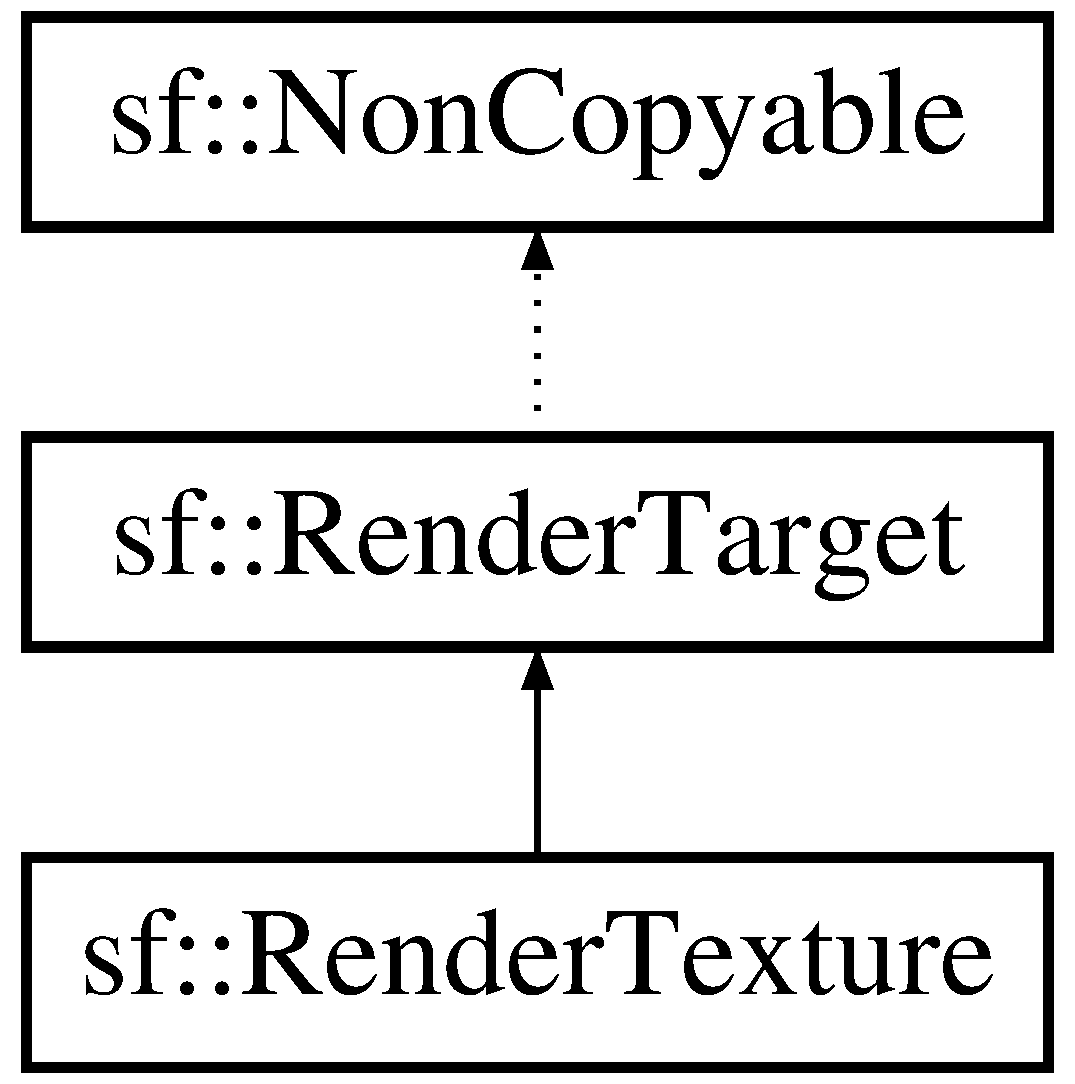
\includegraphics[height=3.000000cm]{classsf_1_1RenderTexture}
\end{center}
\end{figure}
\subsection*{Public Member Functions}
\begin{DoxyCompactItemize}
\item 
\hyperlink{classsf_1_1RenderTexture_a19ee6e5b4c40ad251803389b3953a9c6}{Render\-Texture} ()
\begin{DoxyCompactList}\small\item\em Default constructor. \end{DoxyCompactList}\item 
\hypertarget{classsf_1_1RenderTexture_a94b84ab9335be84d2a014c964d973304}{virtual \hyperlink{classsf_1_1RenderTexture_a94b84ab9335be84d2a014c964d973304}{$\sim$\-Render\-Texture} ()}\label{classsf_1_1RenderTexture_a94b84ab9335be84d2a014c964d973304}

\begin{DoxyCompactList}\small\item\em Destructor. \end{DoxyCompactList}\item 
bool \hyperlink{classsf_1_1RenderTexture_aefbb76eb3b87e368ab974b2660931ccb}{create} (unsigned int width, unsigned int height, bool depth\-Buffer=false)
\begin{DoxyCompactList}\small\item\em Create the render-\/texture. \end{DoxyCompactList}\item 
void \hyperlink{classsf_1_1RenderTexture_af08991e63c6020865dd07b20e27305b6}{set\-Smooth} (bool smooth)
\begin{DoxyCompactList}\small\item\em Enable or disable texture smoothing. \end{DoxyCompactList}\item 
bool \hyperlink{classsf_1_1RenderTexture_ae385f4f4dbd2af50fb11947bf0bcb83d}{is\-Smooth} () const 
\begin{DoxyCompactList}\small\item\em Tell whether the smooth filtering is enabled or not. \end{DoxyCompactList}\item 
void \hyperlink{classsf_1_1RenderTexture_af8f97b33512bf7d5b6be3da6f65f7365}{set\-Repeated} (bool repeated)
\begin{DoxyCompactList}\small\item\em Enable or disable texture repeating. \end{DoxyCompactList}\item 
bool \hyperlink{classsf_1_1RenderTexture_ae480a2ec7ee166afa50232e634d2668c}{is\-Repeated} () const 
\begin{DoxyCompactList}\small\item\em Tell whether the texture is repeated or not. \end{DoxyCompactList}\item 
bool \hyperlink{classsf_1_1RenderTexture_a5da95ecdbce615a80bb78399012508cf}{set\-Active} (bool active=true)
\begin{DoxyCompactList}\small\item\em Activate of deactivate the render-\/texture for rendering. \end{DoxyCompactList}\item 
void \hyperlink{classsf_1_1RenderTexture_af92886d5faef3916caff9fa9ab32c555}{display} ()
\begin{DoxyCompactList}\small\item\em Update the contents of the target texture. \end{DoxyCompactList}\item 
virtual \hyperlink{classsf_1_1Vector2}{Vector2u} \hyperlink{classsf_1_1RenderTexture_a757ba45ec7a7deefcaef717049b00b8c}{get\-Size} () const 
\begin{DoxyCompactList}\small\item\em Return the size of the rendering region of the texture. \end{DoxyCompactList}\item 
const \hyperlink{classsf_1_1Texture}{Texture} \& \hyperlink{classsf_1_1RenderTexture_a95bc5152c497066d31fdc57da8e17678}{get\-Texture} () const 
\begin{DoxyCompactList}\small\item\em Get a read-\/only reference to the target texture. \end{DoxyCompactList}\end{DoxyCompactItemize}
\subsection*{Additional Inherited Members}


\subsection{Detailed Description}
Target for off-\/screen 2\-D rendering into a texture. 

\hyperlink{classsf_1_1RenderTexture}{sf\-::\-Render\-Texture} is the little brother of \hyperlink{classsf_1_1RenderWindow}{sf\-::\-Render\-Window}. It implements the same 2\-D drawing and Open\-G\-L-\/related functions (see their base class \hyperlink{classsf_1_1RenderTarget}{sf\-::\-Render\-Target} for more details), the difference is that the result is stored in an off-\/screen texture rather than being show in a window.

Rendering to a texture can be useful in a variety of situations\-: \begin{DoxyItemize}
\item precomputing a complex static texture (like a level's background from multiple tiles) \item applying post-\/effects to the whole scene with shaders \item creating a sprite from a 3\-D object rendered with Open\-G\-L \item etc.\end{DoxyItemize}
Usage example\-:


\begin{DoxyCode}
\textcolor{comment}{// Create a new render-window}
\hyperlink{classsf_1_1RenderWindow}{sf::RenderWindow} window(\hyperlink{classsf_1_1VideoMode}{sf::VideoMode}(800, 600), \textcolor{stringliteral}{"SFML window"});

\textcolor{comment}{// Create a new render-texture}
\hyperlink{classsf_1_1RenderTexture}{sf::RenderTexture} texture;
\textcolor{keywordflow}{if} (!texture.\hyperlink{classsf_1_1RenderTexture_aefbb76eb3b87e368ab974b2660931ccb}{create}(500, 500))
    \textcolor{keywordflow}{return} -1;

\textcolor{comment}{// The main loop}
\textcolor{keywordflow}{while} (window.isOpen())
\{
   \textcolor{comment}{// Event processing}
   \textcolor{comment}{// ...}

   \textcolor{comment}{// Clear the whole texture with red color}
   texture.\hyperlink{classsf_1_1RenderTarget_a6bb6f0ba348f2b1e2f46114aeaf60f26}{clear}(\hyperlink{classsf_1_1Color_a127dbf55db9c07d0fa8f4bfcbb97594a}{sf::Color::Red});

   \textcolor{comment}{// Draw stuff to the texture}
   texture.\hyperlink{classsf_1_1RenderTarget_a12417a3bcc245c41d957b29583556f39}{draw}(sprite);  \textcolor{comment}{// sprite is a sf::Sprite}
   texture.\hyperlink{classsf_1_1RenderTarget_a12417a3bcc245c41d957b29583556f39}{draw}(shape);   \textcolor{comment}{// shape is a sf::Shape}
   texture.\hyperlink{classsf_1_1RenderTarget_a12417a3bcc245c41d957b29583556f39}{draw}(text);    \textcolor{comment}{// text is a sf::Text}

   \textcolor{comment}{// We're done drawing to the texture}
   texture.\hyperlink{classsf_1_1RenderTexture_af92886d5faef3916caff9fa9ab32c555}{display}();

   \textcolor{comment}{// Now we start rendering to the window, clear it first}
   window.clear();

   \textcolor{comment}{// Draw the texture}
   \hyperlink{classsf_1_1Sprite}{sf::Sprite} sprite(texture.\hyperlink{classsf_1_1RenderTexture_a95bc5152c497066d31fdc57da8e17678}{getTexture}());
   window.draw(sprite);

   \textcolor{comment}{// End the current frame and display its contents on screen}
   window.display();
\}
\end{DoxyCode}


Like \hyperlink{classsf_1_1RenderWindow}{sf\-::\-Render\-Window}, \hyperlink{classsf_1_1RenderTexture}{sf\-::\-Render\-Texture} is still able to render direct Open\-G\-L stuff. It is even possible to mix together Open\-G\-L calls and regular S\-F\-M\-L drawing commands. If you need a depth buffer for 3\-D rendering, don't forget to request it when calling \hyperlink{classsf_1_1RenderTexture_aefbb76eb3b87e368ab974b2660931ccb}{Render\-Texture\-::create}.

\begin{DoxySeeAlso}{See Also}
\hyperlink{classsf_1_1RenderTarget}{sf\-::\-Render\-Target}, \hyperlink{classsf_1_1RenderWindow}{sf\-::\-Render\-Window}, \hyperlink{classsf_1_1View}{sf\-::\-View}, \hyperlink{classsf_1_1Texture}{sf\-::\-Texture} 
\end{DoxySeeAlso}


Definition at line 47 of file Render\-Texture.\-hpp.



\subsection{Constructor \& Destructor Documentation}
\hypertarget{classsf_1_1RenderTexture_a19ee6e5b4c40ad251803389b3953a9c6}{\index{sf\-::\-Render\-Texture@{sf\-::\-Render\-Texture}!Render\-Texture@{Render\-Texture}}
\index{Render\-Texture@{Render\-Texture}!sf::RenderTexture@{sf\-::\-Render\-Texture}}
\subsubsection[{Render\-Texture}]{\setlength{\rightskip}{0pt plus 5cm}sf\-::\-Render\-Texture\-::\-Render\-Texture (
\begin{DoxyParamCaption}
{}
\end{DoxyParamCaption}
)}}\label{classsf_1_1RenderTexture_a19ee6e5b4c40ad251803389b3953a9c6}


Default constructor. 

Constructs an empty, invalid render-\/texture. You must call create to have a valid render-\/texture.

\begin{DoxySeeAlso}{See Also}
\hyperlink{classsf_1_1RenderTexture_aefbb76eb3b87e368ab974b2660931ccb}{create} 
\end{DoxySeeAlso}


\subsection{Member Function Documentation}
\hypertarget{classsf_1_1RenderTexture_aefbb76eb3b87e368ab974b2660931ccb}{\index{sf\-::\-Render\-Texture@{sf\-::\-Render\-Texture}!create@{create}}
\index{create@{create}!sf::RenderTexture@{sf\-::\-Render\-Texture}}
\subsubsection[{create}]{\setlength{\rightskip}{0pt plus 5cm}bool sf\-::\-Render\-Texture\-::create (
\begin{DoxyParamCaption}
\item[{unsigned int}]{width, }
\item[{unsigned int}]{height, }
\item[{bool}]{depth\-Buffer = {\ttfamily false}}
\end{DoxyParamCaption}
)}}\label{classsf_1_1RenderTexture_aefbb76eb3b87e368ab974b2660931ccb}


Create the render-\/texture. 

Before calling this function, the render-\/texture is in an invalid state, thus it is mandatory to call it before doing anything with the render-\/texture. The last parameter, {\itshape depth\-Buffer}, is useful if you want to use the render-\/texture for 3\-D Open\-G\-L rendering that requires a depth-\/buffer. Otherwise it is unnecessary, and you should leave this parameter to false (which is its default value).


\begin{DoxyParams}{Parameters}
{\em width} & Width of the render-\/texture \\
\hline
{\em height} & Height of the render-\/texture \\
\hline
{\em depth\-Buffer} & Do you want this render-\/texture to have a depth buffer?\\
\hline
\end{DoxyParams}
\begin{DoxyReturn}{Returns}
True if creation has been successful 
\end{DoxyReturn}
\hypertarget{classsf_1_1RenderTexture_af92886d5faef3916caff9fa9ab32c555}{\index{sf\-::\-Render\-Texture@{sf\-::\-Render\-Texture}!display@{display}}
\index{display@{display}!sf::RenderTexture@{sf\-::\-Render\-Texture}}
\subsubsection[{display}]{\setlength{\rightskip}{0pt plus 5cm}void sf\-::\-Render\-Texture\-::display (
\begin{DoxyParamCaption}
{}
\end{DoxyParamCaption}
)}}\label{classsf_1_1RenderTexture_af92886d5faef3916caff9fa9ab32c555}


Update the contents of the target texture. 

This function updates the target texture with what has been drawn so far. Like for windows, calling this function is mandatory at the end of rendering. Not calling it may leave the texture in an undefined state. \hypertarget{classsf_1_1RenderTexture_a757ba45ec7a7deefcaef717049b00b8c}{\index{sf\-::\-Render\-Texture@{sf\-::\-Render\-Texture}!get\-Size@{get\-Size}}
\index{get\-Size@{get\-Size}!sf::RenderTexture@{sf\-::\-Render\-Texture}}
\subsubsection[{get\-Size}]{\setlength{\rightskip}{0pt plus 5cm}virtual {\bf Vector2u} sf\-::\-Render\-Texture\-::get\-Size (
\begin{DoxyParamCaption}
{}
\end{DoxyParamCaption}
) const\hspace{0.3cm}{\ttfamily [virtual]}}}\label{classsf_1_1RenderTexture_a757ba45ec7a7deefcaef717049b00b8c}


Return the size of the rendering region of the texture. 

The returned value is the size that you passed to the create function.

\begin{DoxyReturn}{Returns}
Size in pixels 
\end{DoxyReturn}


Implements \hyperlink{classsf_1_1RenderTarget_a2e5ade2457d9fb4c4907ae5b3d9e94a5}{sf\-::\-Render\-Target}.

\hypertarget{classsf_1_1RenderTexture_a95bc5152c497066d31fdc57da8e17678}{\index{sf\-::\-Render\-Texture@{sf\-::\-Render\-Texture}!get\-Texture@{get\-Texture}}
\index{get\-Texture@{get\-Texture}!sf::RenderTexture@{sf\-::\-Render\-Texture}}
\subsubsection[{get\-Texture}]{\setlength{\rightskip}{0pt plus 5cm}const {\bf Texture}\& sf\-::\-Render\-Texture\-::get\-Texture (
\begin{DoxyParamCaption}
{}
\end{DoxyParamCaption}
) const}}\label{classsf_1_1RenderTexture_a95bc5152c497066d31fdc57da8e17678}


Get a read-\/only reference to the target texture. 

After drawing to the render-\/texture and calling Display, you can retrieve the updated texture using this function, and draw it using a sprite (for example). The internal \hyperlink{classsf_1_1Texture}{sf\-::\-Texture} of a render-\/texture is always the same instance, so that it is possible to call this function once and keep a reference to the texture even after it is modified.

\begin{DoxyReturn}{Returns}
Const reference to the texture 
\end{DoxyReturn}
\hypertarget{classsf_1_1RenderTexture_ae480a2ec7ee166afa50232e634d2668c}{\index{sf\-::\-Render\-Texture@{sf\-::\-Render\-Texture}!is\-Repeated@{is\-Repeated}}
\index{is\-Repeated@{is\-Repeated}!sf::RenderTexture@{sf\-::\-Render\-Texture}}
\subsubsection[{is\-Repeated}]{\setlength{\rightskip}{0pt plus 5cm}bool sf\-::\-Render\-Texture\-::is\-Repeated (
\begin{DoxyParamCaption}
{}
\end{DoxyParamCaption}
) const}}\label{classsf_1_1RenderTexture_ae480a2ec7ee166afa50232e634d2668c}


Tell whether the texture is repeated or not. 

\begin{DoxyReturn}{Returns}
True if texture is repeated
\end{DoxyReturn}
\begin{DoxySeeAlso}{See Also}
\hyperlink{classsf_1_1RenderTexture_af8f97b33512bf7d5b6be3da6f65f7365}{set\-Repeated} 
\end{DoxySeeAlso}
\hypertarget{classsf_1_1RenderTexture_ae385f4f4dbd2af50fb11947bf0bcb83d}{\index{sf\-::\-Render\-Texture@{sf\-::\-Render\-Texture}!is\-Smooth@{is\-Smooth}}
\index{is\-Smooth@{is\-Smooth}!sf::RenderTexture@{sf\-::\-Render\-Texture}}
\subsubsection[{is\-Smooth}]{\setlength{\rightskip}{0pt plus 5cm}bool sf\-::\-Render\-Texture\-::is\-Smooth (
\begin{DoxyParamCaption}
{}
\end{DoxyParamCaption}
) const}}\label{classsf_1_1RenderTexture_ae385f4f4dbd2af50fb11947bf0bcb83d}


Tell whether the smooth filtering is enabled or not. 

\begin{DoxyReturn}{Returns}
True if texture smoothing is enabled
\end{DoxyReturn}
\begin{DoxySeeAlso}{See Also}
\hyperlink{classsf_1_1RenderTexture_af08991e63c6020865dd07b20e27305b6}{set\-Smooth} 
\end{DoxySeeAlso}
\hypertarget{classsf_1_1RenderTexture_a5da95ecdbce615a80bb78399012508cf}{\index{sf\-::\-Render\-Texture@{sf\-::\-Render\-Texture}!set\-Active@{set\-Active}}
\index{set\-Active@{set\-Active}!sf::RenderTexture@{sf\-::\-Render\-Texture}}
\subsubsection[{set\-Active}]{\setlength{\rightskip}{0pt plus 5cm}bool sf\-::\-Render\-Texture\-::set\-Active (
\begin{DoxyParamCaption}
\item[{bool}]{active = {\ttfamily true}}
\end{DoxyParamCaption}
)}}\label{classsf_1_1RenderTexture_a5da95ecdbce615a80bb78399012508cf}


Activate of deactivate the render-\/texture for rendering. 

This function makes the render-\/texture's context current for future Open\-G\-L rendering operations (so you shouldn't care about it if you're not doing direct Open\-G\-L stuff). Only one context can be current in a thread, so if you want to draw Open\-G\-L geometry to another render target (like a \hyperlink{classsf_1_1RenderWindow}{Render\-Window}) don't forget to activate it again.


\begin{DoxyParams}{Parameters}
{\em active} & True to activate, false to deactivate\\
\hline
\end{DoxyParams}
\begin{DoxyReturn}{Returns}
True if operation was successful, false otherwise 
\end{DoxyReturn}
\hypertarget{classsf_1_1RenderTexture_af8f97b33512bf7d5b6be3da6f65f7365}{\index{sf\-::\-Render\-Texture@{sf\-::\-Render\-Texture}!set\-Repeated@{set\-Repeated}}
\index{set\-Repeated@{set\-Repeated}!sf::RenderTexture@{sf\-::\-Render\-Texture}}
\subsubsection[{set\-Repeated}]{\setlength{\rightskip}{0pt plus 5cm}void sf\-::\-Render\-Texture\-::set\-Repeated (
\begin{DoxyParamCaption}
\item[{bool}]{repeated}
\end{DoxyParamCaption}
)}}\label{classsf_1_1RenderTexture_af8f97b33512bf7d5b6be3da6f65f7365}


Enable or disable texture repeating. 

This function is similar to \hyperlink{classsf_1_1Texture_aaa87d1eff053b9d4d34a24c784a28658}{Texture\-::set\-Repeated}. This parameter is disabled by default.


\begin{DoxyParams}{Parameters}
{\em repeated} & True to enable repeating, false to disable it\\
\hline
\end{DoxyParams}
\begin{DoxySeeAlso}{See Also}
\hyperlink{classsf_1_1RenderTexture_ae480a2ec7ee166afa50232e634d2668c}{is\-Repeated} 
\end{DoxySeeAlso}
\hypertarget{classsf_1_1RenderTexture_af08991e63c6020865dd07b20e27305b6}{\index{sf\-::\-Render\-Texture@{sf\-::\-Render\-Texture}!set\-Smooth@{set\-Smooth}}
\index{set\-Smooth@{set\-Smooth}!sf::RenderTexture@{sf\-::\-Render\-Texture}}
\subsubsection[{set\-Smooth}]{\setlength{\rightskip}{0pt plus 5cm}void sf\-::\-Render\-Texture\-::set\-Smooth (
\begin{DoxyParamCaption}
\item[{bool}]{smooth}
\end{DoxyParamCaption}
)}}\label{classsf_1_1RenderTexture_af08991e63c6020865dd07b20e27305b6}


Enable or disable texture smoothing. 

This function is similar to \hyperlink{classsf_1_1Texture_a0c3bd6825b9a99714f10d44179d74324}{Texture\-::set\-Smooth}. This parameter is disabled by default.


\begin{DoxyParams}{Parameters}
{\em smooth} & True to enable smoothing, false to disable it\\
\hline
\end{DoxyParams}
\begin{DoxySeeAlso}{See Also}
\hyperlink{classsf_1_1RenderTexture_ae385f4f4dbd2af50fb11947bf0bcb83d}{is\-Smooth} 
\end{DoxySeeAlso}


The documentation for this class was generated from the following file\-:\begin{DoxyCompactItemize}
\item 
/home/z\-Zelman/\-Dropbox/\-Placeholder-\/\-R\-T\-S/\-S\-F\-M\-L-\/2.\-1/include/\-S\-F\-M\-L/\-Graphics/Render\-Texture.\-hpp\end{DoxyCompactItemize}

\hypertarget{classsf_1_1RenderWindow}{\section{sf\-:\-:Render\-Window Class Reference}
\label{classsf_1_1RenderWindow}\index{sf\-::\-Render\-Window@{sf\-::\-Render\-Window}}
}


\hyperlink{classsf_1_1Window}{Window} that can serve as a target for 2\-D drawing.  




{\ttfamily \#include $<$Render\-Window.\-hpp$>$}

Inheritance diagram for sf\-:\-:Render\-Window\-:\begin{figure}[H]
\begin{center}
\leavevmode
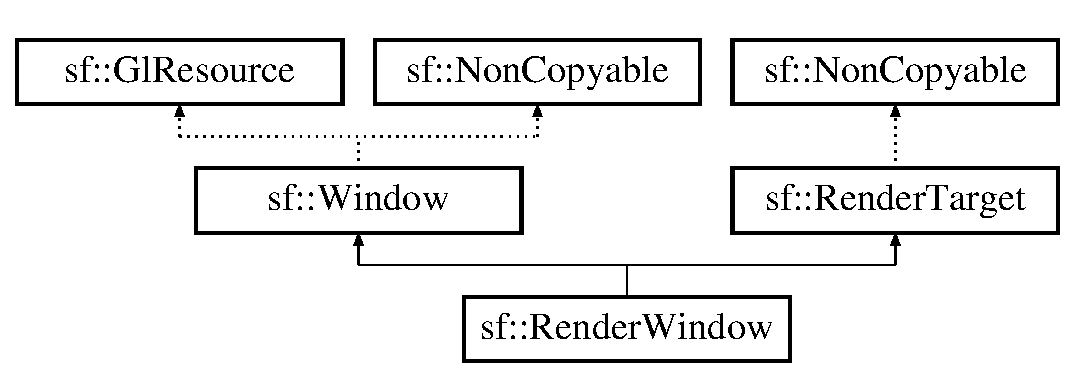
\includegraphics[height=3.000000cm]{classsf_1_1RenderWindow}
\end{center}
\end{figure}
\subsection*{Public Member Functions}
\begin{DoxyCompactItemize}
\item 
\hyperlink{classsf_1_1RenderWindow_a839bbf336bdcafb084dafc3076fc9021}{Render\-Window} ()
\begin{DoxyCompactList}\small\item\em Default constructor. \end{DoxyCompactList}\item 
\hyperlink{classsf_1_1RenderWindow_aebef983e01f677bf5a66cefc4d547647}{Render\-Window} (\hyperlink{classsf_1_1VideoMode}{Video\-Mode} mode, const \hyperlink{classsf_1_1String}{String} \&title, Uint32 style=Style\-::\-Default, const \hyperlink{structsf_1_1ContextSettings}{Context\-Settings} \&settings=\hyperlink{structsf_1_1ContextSettings}{Context\-Settings}())
\begin{DoxyCompactList}\small\item\em Construct a new window. \end{DoxyCompactList}\item 
\hyperlink{classsf_1_1RenderWindow_a25c0af7d515e710b6eebc9c6be952aa5}{Render\-Window} (Window\-Handle handle, const \hyperlink{structsf_1_1ContextSettings}{Context\-Settings} \&settings=\hyperlink{structsf_1_1ContextSettings}{Context\-Settings}())
\begin{DoxyCompactList}\small\item\em Construct the window from an existing control. \end{DoxyCompactList}\item 
virtual \hyperlink{classsf_1_1RenderWindow_a3407e36bfc1752d723140438a825365c}{$\sim$\-Render\-Window} ()
\begin{DoxyCompactList}\small\item\em Destructor. \end{DoxyCompactList}\item 
virtual \hyperlink{classsf_1_1Vector2}{Vector2u} \hyperlink{classsf_1_1RenderWindow_a2c7ff414be32621a453745cf2a0f8a3e}{get\-Size} () const 
\begin{DoxyCompactList}\small\item\em Get the size of the rendering region of the window. \end{DoxyCompactList}\item 
\hyperlink{classsf_1_1Image}{Image} \hyperlink{classsf_1_1RenderWindow_a9bd8655d0bac83145bfc329ea7a6d538}{capture} () const 
\begin{DoxyCompactList}\small\item\em Copy the current contents of the window to an image. \end{DoxyCompactList}\end{DoxyCompactItemize}
\subsection*{Protected Member Functions}
\begin{DoxyCompactItemize}
\item 
virtual void \hyperlink{classsf_1_1RenderWindow_a5bef0040b0fa87bed9fbd459c980d53a}{on\-Create} ()
\begin{DoxyCompactList}\small\item\em Function called after the window has been created. \end{DoxyCompactList}\item 
virtual void \hyperlink{classsf_1_1RenderWindow_a5c85fe482313562d33ffd24a194b6fef}{on\-Resize} ()
\begin{DoxyCompactList}\small\item\em Function called after the window has been resized. \end{DoxyCompactList}\end{DoxyCompactItemize}


\subsection{Detailed Description}
\hyperlink{classsf_1_1Window}{Window} that can serve as a target for 2\-D drawing. 

\hyperlink{classsf_1_1RenderWindow}{sf\-::\-Render\-Window} is the main class of the Graphics module. It defines an O\-S window that can be painted using the other classes of the graphics module.

\hyperlink{classsf_1_1RenderWindow}{sf\-::\-Render\-Window} is derived from \hyperlink{classsf_1_1Window}{sf\-::\-Window}, thus it inherits all its features\-: events, window management, Open\-G\-L rendering, etc. See the documentation of \hyperlink{classsf_1_1Window}{sf\-::\-Window} for a more complete description of all these features, as well as code examples.

On top of that, \hyperlink{classsf_1_1RenderWindow}{sf\-::\-Render\-Window} adds more features related to 2\-D drawing with the graphics module (see its base class \hyperlink{classsf_1_1RenderTarget}{sf\-::\-Render\-Target} for more details). Here is a typical rendering and event loop with a \hyperlink{classsf_1_1RenderWindow}{sf\-::\-Render\-Window}\-:


\begin{DoxyCode}
\textcolor{comment}{// Declare and create a new render-window}
\hyperlink{classsf_1_1RenderWindow}{sf::RenderWindow} window(\hyperlink{classsf_1_1VideoMode}{sf::VideoMode}(800, 600), \textcolor{stringliteral}{"SFML window"});

\textcolor{comment}{// Limit the framerate to 60 frames per second (this step is optional)}
window.setFramerateLimit(60);

\textcolor{comment}{// The main loop - ends as soon as the window is closed}
\textcolor{keywordflow}{while} (window.isOpen())
\{
   \textcolor{comment}{// Event processing}
   \hyperlink{classsf_1_1Event}{sf::Event} event;
   \textcolor{keywordflow}{while} (window.pollEvent(event))
   \{
       \textcolor{comment}{// Request for closing the window}
       \textcolor{keywordflow}{if} (event.\hyperlink{classsf_1_1Event_adf2f8044f713fd9d6019077b0d1ffe0a}{type} == \hyperlink{classsf_1_1Event_af41fa9ed45c02449030699f671331d4aa316e4212e083f1dce79efd8d9e9c0a95}{sf::Event::Closed})
           window.close();
   \}

   \textcolor{comment}{// Clear the whole window before rendering a new frame}
   window.clear();

   \textcolor{comment}{// Draw some graphical entities}
   window.draw(sprite);
   window.draw(circle);
   window.draw(text);

   \textcolor{comment}{// End the current frame and display its contents on screen}
   window.display();
\}
\end{DoxyCode}


Like \hyperlink{classsf_1_1Window}{sf\-::\-Window}, \hyperlink{classsf_1_1RenderWindow}{sf\-::\-Render\-Window} is still able to render direct Open\-G\-L stuff. It is even possible to mix together Open\-G\-L calls and regular S\-F\-M\-L drawing commands.


\begin{DoxyCode}
\textcolor{comment}{// Create the render window}
\hyperlink{classsf_1_1RenderWindow}{sf::RenderWindow} window(\hyperlink{classsf_1_1VideoMode}{sf::VideoMode}(800, 600), \textcolor{stringliteral}{"SFML OpenGL"});

\textcolor{comment}{// Create a sprite and a text to display}
\hyperlink{classsf_1_1Sprite}{sf::Sprite} sprite;
\hyperlink{classsf_1_1Text}{sf::Text} text;
...

\textcolor{comment}{// Perform OpenGL initializations}
glMatrixMode(GL\_PROJECTION);
...

\textcolor{comment}{// Start the rendering loop}
while (window.isOpen())
\{
    \textcolor{comment}{// Process events}
    ...

    \textcolor{comment}{// Draw a background sprite}
    window.pushGLStates();
    window.draw(sprite);
    window.popGLStates();

    \textcolor{comment}{// Draw a 3D object using OpenGL}
    glBegin(GL\_QUADS);
        glVertex3f(...);
        ...
    glEnd();

    \textcolor{comment}{// Draw text on top of the 3D object}
    window.pushGLStates();
    window.draw(text);
    window.popGLStates();

    \textcolor{comment}{// Finally, display the rendered frame on screen}
    window.display();
\}
\end{DoxyCode}


\begin{DoxySeeAlso}{See Also}
\hyperlink{classsf_1_1Window}{sf\-::\-Window}, \hyperlink{classsf_1_1RenderTarget}{sf\-::\-Render\-Target}, \hyperlink{classsf_1_1RenderTexture}{sf\-::\-Render\-Texture}, \hyperlink{classsf_1_1View}{sf\-::\-View} 
\end{DoxySeeAlso}


Definition at line 44 of file Render\-Window.\-hpp.



\subsection{Constructor \& Destructor Documentation}
\hypertarget{classsf_1_1RenderWindow_a839bbf336bdcafb084dafc3076fc9021}{\index{sf\-::\-Render\-Window@{sf\-::\-Render\-Window}!Render\-Window@{Render\-Window}}
\index{Render\-Window@{Render\-Window}!sf::RenderWindow@{sf\-::\-Render\-Window}}
\subsubsection[{Render\-Window}]{\setlength{\rightskip}{0pt plus 5cm}sf\-::\-Render\-Window\-::\-Render\-Window (
\begin{DoxyParamCaption}
{}
\end{DoxyParamCaption}
)}}\label{classsf_1_1RenderWindow_a839bbf336bdcafb084dafc3076fc9021}


Default constructor. 

This constructor doesn't actually create the window, use the other constructors or call \char`\"{}create\char`\"{} to do so. \hypertarget{classsf_1_1RenderWindow_aebef983e01f677bf5a66cefc4d547647}{\index{sf\-::\-Render\-Window@{sf\-::\-Render\-Window}!Render\-Window@{Render\-Window}}
\index{Render\-Window@{Render\-Window}!sf::RenderWindow@{sf\-::\-Render\-Window}}
\subsubsection[{Render\-Window}]{\setlength{\rightskip}{0pt plus 5cm}sf\-::\-Render\-Window\-::\-Render\-Window (
\begin{DoxyParamCaption}
\item[{{\bf Video\-Mode}}]{mode, }
\item[{const {\bf String} \&}]{title, }
\item[{Uint32}]{style = {\ttfamily Style\-:\-:Default}, }
\item[{const {\bf Context\-Settings} \&}]{settings = {\ttfamily {\bf Context\-Settings}()}}
\end{DoxyParamCaption}
)}}\label{classsf_1_1RenderWindow_aebef983e01f677bf5a66cefc4d547647}


Construct a new window. 

This constructor creates the window with the size and pixel depth defined in {\itshape mode}. An optional style can be passed to customize the look and behaviour of the window (borders, title bar, resizable, closable, ...).

The fourth parameter is an optional structure specifying advanced Open\-G\-L context settings such as antialiasing, depth-\/buffer bits, etc. You shouldn't care about these parameters for a regular usage of the graphics module.


\begin{DoxyParams}{Parameters}
{\em mode} & Video mode to use (defines the width, height and depth of the rendering area of the window) \\
\hline
{\em title} & Title of the window \\
\hline
{\em style} & \hyperlink{classsf_1_1Window}{Window} style \\
\hline
{\em settings} & Additional settings for the underlying Open\-G\-L context \\
\hline
\end{DoxyParams}
\hypertarget{classsf_1_1RenderWindow_a25c0af7d515e710b6eebc9c6be952aa5}{\index{sf\-::\-Render\-Window@{sf\-::\-Render\-Window}!Render\-Window@{Render\-Window}}
\index{Render\-Window@{Render\-Window}!sf::RenderWindow@{sf\-::\-Render\-Window}}
\subsubsection[{Render\-Window}]{\setlength{\rightskip}{0pt plus 5cm}sf\-::\-Render\-Window\-::\-Render\-Window (
\begin{DoxyParamCaption}
\item[{Window\-Handle}]{handle, }
\item[{const {\bf Context\-Settings} \&}]{settings = {\ttfamily {\bf Context\-Settings}()}}
\end{DoxyParamCaption}
)\hspace{0.3cm}{\ttfamily [explicit]}}}\label{classsf_1_1RenderWindow_a25c0af7d515e710b6eebc9c6be952aa5}


Construct the window from an existing control. 

Use this constructor if you want to create an S\-F\-M\-L rendering area into an already existing control.

The fourth parameter is an optional structure specifying advanced Open\-G\-L context settings such as antialiasing, depth-\/buffer bits, etc. You shouldn't care about these parameters for a regular usage of the graphics module.


\begin{DoxyParams}{Parameters}
{\em handle} & Platform-\/specific handle of the control \\
\hline
{\em settings} & Additional settings for the underlying Open\-G\-L context \\
\hline
\end{DoxyParams}
\hypertarget{classsf_1_1RenderWindow_a3407e36bfc1752d723140438a825365c}{\index{sf\-::\-Render\-Window@{sf\-::\-Render\-Window}!$\sim$\-Render\-Window@{$\sim$\-Render\-Window}}
\index{$\sim$\-Render\-Window@{$\sim$\-Render\-Window}!sf::RenderWindow@{sf\-::\-Render\-Window}}
\subsubsection[{$\sim$\-Render\-Window}]{\setlength{\rightskip}{0pt plus 5cm}virtual sf\-::\-Render\-Window\-::$\sim$\-Render\-Window (
\begin{DoxyParamCaption}
{}
\end{DoxyParamCaption}
)\hspace{0.3cm}{\ttfamily [virtual]}}}\label{classsf_1_1RenderWindow_a3407e36bfc1752d723140438a825365c}


Destructor. 

Closes the window and free all the resources attached to it. 

\subsection{Member Function Documentation}
\hypertarget{classsf_1_1RenderWindow_a9bd8655d0bac83145bfc329ea7a6d538}{\index{sf\-::\-Render\-Window@{sf\-::\-Render\-Window}!capture@{capture}}
\index{capture@{capture}!sf::RenderWindow@{sf\-::\-Render\-Window}}
\subsubsection[{capture}]{\setlength{\rightskip}{0pt plus 5cm}{\bf Image} sf\-::\-Render\-Window\-::capture (
\begin{DoxyParamCaption}
{}
\end{DoxyParamCaption}
) const}}\label{classsf_1_1RenderWindow_a9bd8655d0bac83145bfc329ea7a6d538}


Copy the current contents of the window to an image. 

This is a slow operation, whose main purpose is to make screenshots of the application. If you want to update an image with the contents of the window and then use it for drawing, you should rather use a \hyperlink{classsf_1_1Texture}{sf\-::\-Texture} and its update(\-Window\&) function. You can also draw things directly to a texture with the \hyperlink{classsf_1_1RenderTexture}{sf\-::\-Render\-Texture} class.

\begin{DoxyReturn}{Returns}
\hyperlink{classsf_1_1Image}{Image} containing the captured contents 
\end{DoxyReturn}
\hypertarget{classsf_1_1RenderWindow_a2c7ff414be32621a453745cf2a0f8a3e}{\index{sf\-::\-Render\-Window@{sf\-::\-Render\-Window}!get\-Size@{get\-Size}}
\index{get\-Size@{get\-Size}!sf::RenderWindow@{sf\-::\-Render\-Window}}
\subsubsection[{get\-Size}]{\setlength{\rightskip}{0pt plus 5cm}virtual {\bf Vector2u} sf\-::\-Render\-Window\-::get\-Size (
\begin{DoxyParamCaption}
{}
\end{DoxyParamCaption}
) const\hspace{0.3cm}{\ttfamily [virtual]}}}\label{classsf_1_1RenderWindow_a2c7ff414be32621a453745cf2a0f8a3e}


Get the size of the rendering region of the window. 

The size doesn't include the titlebar and borders of the window.

\begin{DoxyReturn}{Returns}
Size in pixels 
\end{DoxyReturn}


Implements \hyperlink{classsf_1_1RenderTarget_a2e5ade2457d9fb4c4907ae5b3d9e94a5}{sf\-::\-Render\-Target}.

\hypertarget{classsf_1_1RenderWindow_a5bef0040b0fa87bed9fbd459c980d53a}{\index{sf\-::\-Render\-Window@{sf\-::\-Render\-Window}!on\-Create@{on\-Create}}
\index{on\-Create@{on\-Create}!sf::RenderWindow@{sf\-::\-Render\-Window}}
\subsubsection[{on\-Create}]{\setlength{\rightskip}{0pt plus 5cm}virtual void sf\-::\-Render\-Window\-::on\-Create (
\begin{DoxyParamCaption}
{}
\end{DoxyParamCaption}
)\hspace{0.3cm}{\ttfamily [protected]}, {\ttfamily [virtual]}}}\label{classsf_1_1RenderWindow_a5bef0040b0fa87bed9fbd459c980d53a}


Function called after the window has been created. 

This function is called so that derived classes can perform their own specific initialization as soon as the window is created. 

Reimplemented from \hyperlink{classsf_1_1Window_a106633b9be49b27f83d4712689b493eb}{sf\-::\-Window}.

\hypertarget{classsf_1_1RenderWindow_a5c85fe482313562d33ffd24a194b6fef}{\index{sf\-::\-Render\-Window@{sf\-::\-Render\-Window}!on\-Resize@{on\-Resize}}
\index{on\-Resize@{on\-Resize}!sf::RenderWindow@{sf\-::\-Render\-Window}}
\subsubsection[{on\-Resize}]{\setlength{\rightskip}{0pt plus 5cm}virtual void sf\-::\-Render\-Window\-::on\-Resize (
\begin{DoxyParamCaption}
{}
\end{DoxyParamCaption}
)\hspace{0.3cm}{\ttfamily [protected]}, {\ttfamily [virtual]}}}\label{classsf_1_1RenderWindow_a5c85fe482313562d33ffd24a194b6fef}


Function called after the window has been resized. 

This function is called so that derived classes can perform custom actions when the size of the window changes. 

Reimplemented from \hyperlink{classsf_1_1Window_a10f567a387da7b49f417f73321fcf64d}{sf\-::\-Window}.



The documentation for this class was generated from the following file\-:\begin{DoxyCompactItemize}
\item 
/home/z\-Zelman/\-Dropbox/\-Placeholder-\/\-R\-T\-S/\-S\-F\-M\-L-\/2.\-1/include/\-S\-F\-M\-L/\-Graphics/Render\-Window.\-hpp\end{DoxyCompactItemize}

\hypertarget{classsf_1_1Http_1_1Request}{\section{sf\-:\-:Http\-:\-:Request Class Reference}
\label{classsf_1_1Http_1_1Request}\index{sf\-::\-Http\-::\-Request@{sf\-::\-Http\-::\-Request}}
}


Define a H\-T\-T\-P request.  




{\ttfamily \#include $<$Http.\-hpp$>$}

\subsection*{Public Types}
\begin{DoxyCompactItemize}
\item 
enum \hyperlink{classsf_1_1Http_1_1Request_a620f8bff6f43e1378f321bf53fbf5598}{Method} \{ \hyperlink{classsf_1_1Http_1_1Request_a620f8bff6f43e1378f321bf53fbf5598ab822baed393f3d0353621e5378b9fcb4}{Get}, 
\hyperlink{classsf_1_1Http_1_1Request_a620f8bff6f43e1378f321bf53fbf5598ae8ec4048b9550f8d0747d4199603141a}{Post}, 
\hyperlink{classsf_1_1Http_1_1Request_a620f8bff6f43e1378f321bf53fbf5598a4df23138be7ed60f47aba6548ba65e7b}{Head}
 \}
\begin{DoxyCompactList}\small\item\em Enumerate the available H\-T\-T\-P methods for a request. \end{DoxyCompactList}\end{DoxyCompactItemize}
\subsection*{Public Member Functions}
\begin{DoxyCompactItemize}
\item 
\hyperlink{classsf_1_1Http_1_1Request_a8e89d9e8ffcc1163259b35d79809a61c}{Request} (const std\-::string \&uri=\char`\"{}/\char`\"{}, \hyperlink{classsf_1_1Http_1_1Request_a620f8bff6f43e1378f321bf53fbf5598}{Method} method=\hyperlink{classsf_1_1Http_1_1Request_a620f8bff6f43e1378f321bf53fbf5598ab822baed393f3d0353621e5378b9fcb4}{Get}, const std\-::string \&body=\char`\"{}\char`\"{})
\begin{DoxyCompactList}\small\item\em Default constructor. \end{DoxyCompactList}\item 
void \hyperlink{classsf_1_1Http_1_1Request_aea672fae5dd089f4b6b3745ed46210d2}{set\-Field} (const std\-::string \&field, const std\-::string \&value)
\begin{DoxyCompactList}\small\item\em Set the value of a field. \end{DoxyCompactList}\item 
void \hyperlink{classsf_1_1Http_1_1Request_abab148554e873e80d2e41376fde1cb62}{set\-Method} (\hyperlink{classsf_1_1Http_1_1Request_a620f8bff6f43e1378f321bf53fbf5598}{Method} method)
\begin{DoxyCompactList}\small\item\em Set the request method. \end{DoxyCompactList}\item 
void \hyperlink{classsf_1_1Http_1_1Request_a3723de4b4f1a14b744477841c4ac22e6}{set\-Uri} (const std\-::string \&uri)
\begin{DoxyCompactList}\small\item\em Set the requested U\-R\-I. \end{DoxyCompactList}\item 
void \hyperlink{classsf_1_1Http_1_1Request_aa683b607b737a6224a91387b4108d3c7}{set\-Http\-Version} (unsigned int major, unsigned int minor)
\begin{DoxyCompactList}\small\item\em Set the H\-T\-T\-P version for the request. \end{DoxyCompactList}\item 
void \hyperlink{classsf_1_1Http_1_1Request_ae9f61ec3fa1639c70e9b5780cb35578e}{set\-Body} (const std\-::string \&body)
\begin{DoxyCompactList}\small\item\em Set the body of the request. \end{DoxyCompactList}\end{DoxyCompactItemize}
\subsection*{Friends}
\begin{DoxyCompactItemize}
\item 
\hypertarget{classsf_1_1Http_1_1Request_aba95e2a7762bb5df986048b05d03a22e}{class {\bfseries Http}}\label{classsf_1_1Http_1_1Request_aba95e2a7762bb5df986048b05d03a22e}

\end{DoxyCompactItemize}


\subsection{Detailed Description}
Define a H\-T\-T\-P request. 

Definition at line 54 of file Http.\-hpp.



\subsection{Member Enumeration Documentation}
\hypertarget{classsf_1_1Http_1_1Request_a620f8bff6f43e1378f321bf53fbf5598}{\index{sf\-::\-Http\-::\-Request@{sf\-::\-Http\-::\-Request}!Method@{Method}}
\index{Method@{Method}!sf::Http::Request@{sf\-::\-Http\-::\-Request}}
\subsubsection[{Method}]{\setlength{\rightskip}{0pt plus 5cm}enum {\bf sf\-::\-Http\-::\-Request\-::\-Method}}}\label{classsf_1_1Http_1_1Request_a620f8bff6f43e1378f321bf53fbf5598}


Enumerate the available H\-T\-T\-P methods for a request. 

\begin{Desc}
\item[Enumerator]\par
\begin{description}
\index{Get@{Get}!sf\-::\-Http\-::\-Request@{sf\-::\-Http\-::\-Request}}\index{sf\-::\-Http\-::\-Request@{sf\-::\-Http\-::\-Request}!Get@{Get}}\item[{\em 
\hypertarget{classsf_1_1Http_1_1Request_a620f8bff6f43e1378f321bf53fbf5598ab822baed393f3d0353621e5378b9fcb4}{Get}\label{classsf_1_1Http_1_1Request_a620f8bff6f43e1378f321bf53fbf5598ab822baed393f3d0353621e5378b9fcb4}
}]\hyperlink{classsf_1_1Http_1_1Request}{Request} in get mode, standard method to retrieve a page. \index{Post@{Post}!sf\-::\-Http\-::\-Request@{sf\-::\-Http\-::\-Request}}\index{sf\-::\-Http\-::\-Request@{sf\-::\-Http\-::\-Request}!Post@{Post}}\item[{\em 
\hypertarget{classsf_1_1Http_1_1Request_a620f8bff6f43e1378f321bf53fbf5598ae8ec4048b9550f8d0747d4199603141a}{Post}\label{classsf_1_1Http_1_1Request_a620f8bff6f43e1378f321bf53fbf5598ae8ec4048b9550f8d0747d4199603141a}
}]\hyperlink{classsf_1_1Http_1_1Request}{Request} in post mode, usually to send data to a page. \index{Head@{Head}!sf\-::\-Http\-::\-Request@{sf\-::\-Http\-::\-Request}}\index{sf\-::\-Http\-::\-Request@{sf\-::\-Http\-::\-Request}!Head@{Head}}\item[{\em 
\hypertarget{classsf_1_1Http_1_1Request_a620f8bff6f43e1378f321bf53fbf5598a4df23138be7ed60f47aba6548ba65e7b}{Head}\label{classsf_1_1Http_1_1Request_a620f8bff6f43e1378f321bf53fbf5598a4df23138be7ed60f47aba6548ba65e7b}
}]\hyperlink{classsf_1_1Http_1_1Request}{Request} a page's header only. \end{description}
\end{Desc}


Definition at line 62 of file Http.\-hpp.



\subsection{Constructor \& Destructor Documentation}
\hypertarget{classsf_1_1Http_1_1Request_a8e89d9e8ffcc1163259b35d79809a61c}{\index{sf\-::\-Http\-::\-Request@{sf\-::\-Http\-::\-Request}!Request@{Request}}
\index{Request@{Request}!sf::Http::Request@{sf\-::\-Http\-::\-Request}}
\subsubsection[{Request}]{\setlength{\rightskip}{0pt plus 5cm}sf\-::\-Http\-::\-Request\-::\-Request (
\begin{DoxyParamCaption}
\item[{const std\-::string \&}]{uri = {\ttfamily \char`\"{}/\char`\"{}}, }
\item[{{\bf Method}}]{method = {\ttfamily {\bf Get}}, }
\item[{const std\-::string \&}]{body = {\ttfamily \char`\"{}\char`\"{}}}
\end{DoxyParamCaption}
)}}\label{classsf_1_1Http_1_1Request_a8e89d9e8ffcc1163259b35d79809a61c}


Default constructor. 

This constructor creates a G\-E\-T request, with the root U\-R\-I (\char`\"{}/\char`\"{}) and an empty body.


\begin{DoxyParams}{Parameters}
{\em uri} & Target U\-R\-I \\
\hline
{\em method} & Method to use for the request \\
\hline
{\em body} & Content of the request's body \\
\hline
\end{DoxyParams}


\subsection{Member Function Documentation}
\hypertarget{classsf_1_1Http_1_1Request_ae9f61ec3fa1639c70e9b5780cb35578e}{\index{sf\-::\-Http\-::\-Request@{sf\-::\-Http\-::\-Request}!set\-Body@{set\-Body}}
\index{set\-Body@{set\-Body}!sf::Http::Request@{sf\-::\-Http\-::\-Request}}
\subsubsection[{set\-Body}]{\setlength{\rightskip}{0pt plus 5cm}void sf\-::\-Http\-::\-Request\-::set\-Body (
\begin{DoxyParamCaption}
\item[{const std\-::string \&}]{body}
\end{DoxyParamCaption}
)}}\label{classsf_1_1Http_1_1Request_ae9f61ec3fa1639c70e9b5780cb35578e}


Set the body of the request. 

The body of a request is optional and only makes sense for P\-O\-S\-T requests. It is ignored for all other methods. The body is empty by default.


\begin{DoxyParams}{Parameters}
{\em body} & Content of the body \\
\hline
\end{DoxyParams}
\hypertarget{classsf_1_1Http_1_1Request_aea672fae5dd089f4b6b3745ed46210d2}{\index{sf\-::\-Http\-::\-Request@{sf\-::\-Http\-::\-Request}!set\-Field@{set\-Field}}
\index{set\-Field@{set\-Field}!sf::Http::Request@{sf\-::\-Http\-::\-Request}}
\subsubsection[{set\-Field}]{\setlength{\rightskip}{0pt plus 5cm}void sf\-::\-Http\-::\-Request\-::set\-Field (
\begin{DoxyParamCaption}
\item[{const std\-::string \&}]{field, }
\item[{const std\-::string \&}]{value}
\end{DoxyParamCaption}
)}}\label{classsf_1_1Http_1_1Request_aea672fae5dd089f4b6b3745ed46210d2}


Set the value of a field. 

The field is created if it doesn't exist. The name of the field is case insensitive. By default, a request doesn't contain any field (but the mandatory fields are added later by the H\-T\-T\-P client when sending the request).


\begin{DoxyParams}{Parameters}
{\em field} & Name of the field to set \\
\hline
{\em value} & Value of the field \\
\hline
\end{DoxyParams}
\hypertarget{classsf_1_1Http_1_1Request_aa683b607b737a6224a91387b4108d3c7}{\index{sf\-::\-Http\-::\-Request@{sf\-::\-Http\-::\-Request}!set\-Http\-Version@{set\-Http\-Version}}
\index{set\-Http\-Version@{set\-Http\-Version}!sf::Http::Request@{sf\-::\-Http\-::\-Request}}
\subsubsection[{set\-Http\-Version}]{\setlength{\rightskip}{0pt plus 5cm}void sf\-::\-Http\-::\-Request\-::set\-Http\-Version (
\begin{DoxyParamCaption}
\item[{unsigned int}]{major, }
\item[{unsigned int}]{minor}
\end{DoxyParamCaption}
)}}\label{classsf_1_1Http_1_1Request_aa683b607b737a6224a91387b4108d3c7}


Set the H\-T\-T\-P version for the request. 

The H\-T\-T\-P version is 1.\-0 by default.


\begin{DoxyParams}{Parameters}
{\em major} & Major H\-T\-T\-P version number \\
\hline
{\em minor} & Minor H\-T\-T\-P version number \\
\hline
\end{DoxyParams}
\hypertarget{classsf_1_1Http_1_1Request_abab148554e873e80d2e41376fde1cb62}{\index{sf\-::\-Http\-::\-Request@{sf\-::\-Http\-::\-Request}!set\-Method@{set\-Method}}
\index{set\-Method@{set\-Method}!sf::Http::Request@{sf\-::\-Http\-::\-Request}}
\subsubsection[{set\-Method}]{\setlength{\rightskip}{0pt plus 5cm}void sf\-::\-Http\-::\-Request\-::set\-Method (
\begin{DoxyParamCaption}
\item[{{\bf Method}}]{method}
\end{DoxyParamCaption}
)}}\label{classsf_1_1Http_1_1Request_abab148554e873e80d2e41376fde1cb62}


Set the request method. 

See the Method enumeration for a complete list of all the availale methods. The method is \hyperlink{classsf_1_1Http_1_1Request_a620f8bff6f43e1378f321bf53fbf5598ab822baed393f3d0353621e5378b9fcb4}{Http\-::\-Request\-::\-Get} by default.


\begin{DoxyParams}{Parameters}
{\em method} & Method to use for the request \\
\hline
\end{DoxyParams}
\hypertarget{classsf_1_1Http_1_1Request_a3723de4b4f1a14b744477841c4ac22e6}{\index{sf\-::\-Http\-::\-Request@{sf\-::\-Http\-::\-Request}!set\-Uri@{set\-Uri}}
\index{set\-Uri@{set\-Uri}!sf::Http::Request@{sf\-::\-Http\-::\-Request}}
\subsubsection[{set\-Uri}]{\setlength{\rightskip}{0pt plus 5cm}void sf\-::\-Http\-::\-Request\-::set\-Uri (
\begin{DoxyParamCaption}
\item[{const std\-::string \&}]{uri}
\end{DoxyParamCaption}
)}}\label{classsf_1_1Http_1_1Request_a3723de4b4f1a14b744477841c4ac22e6}


Set the requested U\-R\-I. 

The U\-R\-I is the resource (usually a web page or a file) that you want to get or post. The U\-R\-I is \char`\"{}/\char`\"{} (the root page) by default.


\begin{DoxyParams}{Parameters}
{\em uri} & U\-R\-I to request, relative to the host \\
\hline
\end{DoxyParams}


The documentation for this class was generated from the following file\-:\begin{DoxyCompactItemize}
\item 
/home/z\-Zelman/\-Dropbox/\-Placeholder-\/\-R\-T\-S/\-S\-F\-M\-L-\/2.\-1/include/\-S\-F\-M\-L/\-Network/Http.\-hpp\end{DoxyCompactItemize}

\hypertarget{classsf_1_1Ftp_1_1Response}{\section{sf\-:\-:Ftp\-:\-:Response Class Reference}
\label{classsf_1_1Ftp_1_1Response}\index{sf\-::\-Ftp\-::\-Response@{sf\-::\-Ftp\-::\-Response}}
}


Define a F\-T\-P response.  




{\ttfamily \#include $<$Ftp.\-hpp$>$}

Inheritance diagram for sf\-:\-:Ftp\-:\-:Response\-:\begin{figure}[H]
\begin{center}
\leavevmode
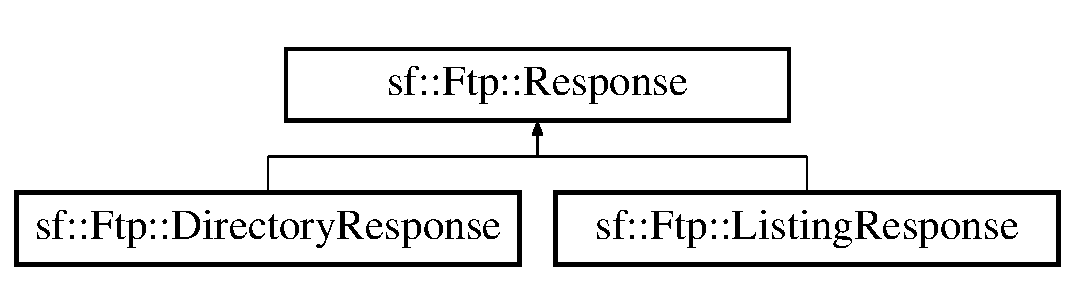
\includegraphics[height=2.000000cm]{classsf_1_1Ftp_1_1Response}
\end{center}
\end{figure}
\subsection*{Public Types}
\begin{DoxyCompactItemize}
\item 
enum \hyperlink{classsf_1_1Ftp_1_1Response_af81738f06b6f571761696291276acb3b}{Status} \{ \\*
\hyperlink{classsf_1_1Ftp_1_1Response_af81738f06b6f571761696291276acb3ba07e06d3326ba2d078583bef93930d909}{Restart\-Marker\-Reply} = 110, 
\hyperlink{classsf_1_1Ftp_1_1Response_af81738f06b6f571761696291276acb3ba22413357ade6b586f6ceb0d704f35075}{Service\-Ready\-Soon} = 120, 
\hyperlink{classsf_1_1Ftp_1_1Response_af81738f06b6f571761696291276acb3bafa52d19bc813d69055f4cc390d4a76ca}{Data\-Connection\-Already\-Opened} = 125, 
\hyperlink{classsf_1_1Ftp_1_1Response_af81738f06b6f571761696291276acb3ba794ebe743688be611447638bf9e49d86}{Opening\-Data\-Connection} = 150, 
\\*
\hyperlink{classsf_1_1Ftp_1_1Response_af81738f06b6f571761696291276acb3baa956e229ba6c0cdf0d88b0e05b286210}{Ok} = 200, 
\hyperlink{classsf_1_1Ftp_1_1Response_af81738f06b6f571761696291276acb3ba38adc424f1adcd332745de8cd3b7737a}{Pointless\-Command} = 202, 
\hyperlink{classsf_1_1Ftp_1_1Response_af81738f06b6f571761696291276acb3ba9bdd02ae119b8be639e778859ee74060}{System\-Status} = 211, 
\hyperlink{classsf_1_1Ftp_1_1Response_af81738f06b6f571761696291276acb3ba8729460a695013cc96330e2fced0ae1f}{Directory\-Status} = 212, 
\\*
\hyperlink{classsf_1_1Ftp_1_1Response_af81738f06b6f571761696291276acb3baebddfc7997dca289c83068dff3f47dce}{File\-Status} = 213, 
\hyperlink{classsf_1_1Ftp_1_1Response_af81738f06b6f571761696291276acb3ba840fd2a1872fd4310b046541f57fdeb7}{Help\-Message} = 214, 
\hyperlink{classsf_1_1Ftp_1_1Response_af81738f06b6f571761696291276acb3ba78391f73aa11f07f1514c7d070b93c08}{System\-Type} = 215, 
\hyperlink{classsf_1_1Ftp_1_1Response_af81738f06b6f571761696291276acb3baea2ee2007d7843c21108bb686ef03757}{Service\-Ready} = 220, 
\\*
\hyperlink{classsf_1_1Ftp_1_1Response_af81738f06b6f571761696291276acb3bab23931490fc2d1df3081d651fe0f4d6e}{Closing\-Connection} = 221, 
\hyperlink{classsf_1_1Ftp_1_1Response_af81738f06b6f571761696291276acb3badc78ed87d5bddb174fa3c16707ac2f2d}{Data\-Connection\-Opened} = 225, 
\hyperlink{classsf_1_1Ftp_1_1Response_af81738f06b6f571761696291276acb3bac723ebc8a38913bbf0d9504556cbaaa6}{Closing\-Data\-Connection} = 226, 
\hyperlink{classsf_1_1Ftp_1_1Response_af81738f06b6f571761696291276acb3ba48314fc47a72ad0aacdea93b91756f6e}{Entering\-Passive\-Mode} = 227, 
\\*
\hyperlink{classsf_1_1Ftp_1_1Response_af81738f06b6f571761696291276acb3ba54a88210386cb72e35d737813a221754}{Logged\-In} = 230, 
\hyperlink{classsf_1_1Ftp_1_1Response_af81738f06b6f571761696291276acb3baf988b69b0a5f55f8122da5ba001932e0}{File\-Action\-Ok} = 250, 
\hyperlink{classsf_1_1Ftp_1_1Response_af81738f06b6f571761696291276acb3ba06d26e95a170fc422af13def415e0437}{Directory\-Ok} = 257, 
\hyperlink{classsf_1_1Ftp_1_1Response_af81738f06b6f571761696291276acb3ba9249e3fe9818eb93f181fbbf3ae3bc56}{Need\-Password} = 331, 
\\*
\hyperlink{classsf_1_1Ftp_1_1Response_af81738f06b6f571761696291276acb3ba9e048185f253f6eb6f5ff9e063b712fa}{Need\-Account\-To\-Log\-In} = 332, 
\hyperlink{classsf_1_1Ftp_1_1Response_af81738f06b6f571761696291276acb3ba02e6f05964ecb829e9b6fb6020d6528a}{Need\-Information} = 350, 
\hyperlink{classsf_1_1Ftp_1_1Response_af81738f06b6f571761696291276acb3ba43022ddf49b68a4f5aff0bea7e09e89f}{Service\-Unavailable} = 421, 
\hyperlink{classsf_1_1Ftp_1_1Response_af81738f06b6f571761696291276acb3ba757b89ff1f236941f7759b0ed0c28b88}{Data\-Connection\-Unavailable} = 425, 
\\*
\hyperlink{classsf_1_1Ftp_1_1Response_af81738f06b6f571761696291276acb3ba7cfefcc586c12ba70f752353fde7126e}{Transfer\-Aborted} = 426, 
\hyperlink{classsf_1_1Ftp_1_1Response_af81738f06b6f571761696291276acb3baf822d1b0abf3e9ae7dd44684549d512d}{File\-Action\-Aborted} = 450, 
\hyperlink{classsf_1_1Ftp_1_1Response_af81738f06b6f571761696291276acb3bae54e84baaca95a7b36271ca3f3fdb900}{Local\-Error} = 451, 
\hyperlink{classsf_1_1Ftp_1_1Response_af81738f06b6f571761696291276acb3ba5d9f3666222c808553c27e4e099c7c6d}{Insufficient\-Storage\-Space} = 452, 
\\*
\hyperlink{classsf_1_1Ftp_1_1Response_af81738f06b6f571761696291276acb3ba75bdf0b6844fa9c07b3c25647d22c269}{Command\-Unknown} = 500, 
\hyperlink{classsf_1_1Ftp_1_1Response_af81738f06b6f571761696291276acb3baf4c7c88815981bbb7c3a3461f9f48b67}{Parameters\-Unknown} = 501, 
\hyperlink{classsf_1_1Ftp_1_1Response_af81738f06b6f571761696291276acb3ba2ca4834c756c81b924ebed696fcba0a8}{Command\-Not\-Implemented} = 502, 
\hyperlink{classsf_1_1Ftp_1_1Response_af81738f06b6f571761696291276acb3bad0c7ab07f01c1f7af16a1852650d7c47}{Bad\-Command\-Sequence} = 503, 
\\*
\hyperlink{classsf_1_1Ftp_1_1Response_af81738f06b6f571761696291276acb3ba8807473b8590e1debfb3740b7a3d081c}{Parameter\-Not\-Implemented} = 504, 
\hyperlink{classsf_1_1Ftp_1_1Response_af81738f06b6f571761696291276acb3bafcfbaff2c6fed941b6bcbc0999db764e}{Not\-Logged\-In} = 530, 
\hyperlink{classsf_1_1Ftp_1_1Response_af81738f06b6f571761696291276acb3ba1af0f173062a471739b50d8e0f40d5f7}{Need\-Account\-To\-Store} = 532, 
\hyperlink{classsf_1_1Ftp_1_1Response_af81738f06b6f571761696291276acb3ba3f8f931e499936fde6b750d81f5ecfef}{File\-Unavailable} = 550, 
\\*
\hyperlink{classsf_1_1Ftp_1_1Response_af81738f06b6f571761696291276acb3bad220bc12dc45593af6e5079ea6c532c3}{Page\-Type\-Unknown} = 551, 
\hyperlink{classsf_1_1Ftp_1_1Response_af81738f06b6f571761696291276acb3baf418e54753e0b8f9cb0325dd618acd14}{Not\-Enough\-Memory} = 552, 
\hyperlink{classsf_1_1Ftp_1_1Response_af81738f06b6f571761696291276acb3ba03254aba823298179a98056e15568c5b}{Filename\-Not\-Allowed} = 553, 
\hyperlink{classsf_1_1Ftp_1_1Response_af81738f06b6f571761696291276acb3ba59e041e4ef186e8ae8d6035973fc46bd}{Invalid\-Response} = 1000, 
\\*
\hyperlink{classsf_1_1Ftp_1_1Response_af81738f06b6f571761696291276acb3ba51aa367cc1e85a45ea3c7be48730e990}{Connection\-Failed} = 1001, 
\hyperlink{classsf_1_1Ftp_1_1Response_af81738f06b6f571761696291276acb3bad1e5dcf298ce30c528261435f1a2eb53}{Connection\-Closed} = 1002, 
\hyperlink{classsf_1_1Ftp_1_1Response_af81738f06b6f571761696291276acb3baed2c74a9f335dee1463ca1a4f41c6478}{Invalid\-File} = 1003
 \}
\begin{DoxyCompactList}\small\item\em Status codes possibly returned by a F\-T\-P response. \end{DoxyCompactList}\end{DoxyCompactItemize}
\subsection*{Public Member Functions}
\begin{DoxyCompactItemize}
\item 
\hyperlink{classsf_1_1Ftp_1_1Response_af300fffd4862774102f978eb22f85d9b}{Response} (\hyperlink{classsf_1_1Ftp_1_1Response_af81738f06b6f571761696291276acb3b}{Status} code=\hyperlink{classsf_1_1Ftp_1_1Response_af81738f06b6f571761696291276acb3ba59e041e4ef186e8ae8d6035973fc46bd}{Invalid\-Response}, const std\-::string \&message=\char`\"{}\char`\"{})
\begin{DoxyCompactList}\small\item\em Default constructor. \end{DoxyCompactList}\item 
bool \hyperlink{classsf_1_1Ftp_1_1Response_a4dadbe0fe0a3ef2d571a017e1645e675}{is\-Ok} () const 
\begin{DoxyCompactList}\small\item\em Check if the status code means a success. \end{DoxyCompactList}\item 
\hyperlink{classsf_1_1Ftp_1_1Response_af81738f06b6f571761696291276acb3b}{Status} \hyperlink{classsf_1_1Ftp_1_1Response_ac7f937b3883d1c4fbc75c003a1786aaa}{get\-Status} () const 
\begin{DoxyCompactList}\small\item\em Get the status code of the response. \end{DoxyCompactList}\item 
const std\-::string \& \hyperlink{classsf_1_1Ftp_1_1Response_a0015675c528a4a84a671484b9e5499d6}{get\-Message} () const 
\begin{DoxyCompactList}\small\item\em Get the full message contained in the response. \end{DoxyCompactList}\end{DoxyCompactItemize}


\subsection{Detailed Description}
Define a F\-T\-P response. 

Definition at line 66 of file Ftp.\-hpp.



\subsection{Member Enumeration Documentation}
\hypertarget{classsf_1_1Ftp_1_1Response_af81738f06b6f571761696291276acb3b}{\index{sf\-::\-Ftp\-::\-Response@{sf\-::\-Ftp\-::\-Response}!Status@{Status}}
\index{Status@{Status}!sf::Ftp::Response@{sf\-::\-Ftp\-::\-Response}}
\subsubsection[{Status}]{\setlength{\rightskip}{0pt plus 5cm}enum {\bf sf\-::\-Ftp\-::\-Response\-::\-Status}}}\label{classsf_1_1Ftp_1_1Response_af81738f06b6f571761696291276acb3b}


Status codes possibly returned by a F\-T\-P response. 

\begin{Desc}
\item[Enumerator]\par
\begin{description}
\index{Restart\-Marker\-Reply@{Restart\-Marker\-Reply}!sf\-::\-Ftp\-::\-Response@{sf\-::\-Ftp\-::\-Response}}\index{sf\-::\-Ftp\-::\-Response@{sf\-::\-Ftp\-::\-Response}!Restart\-Marker\-Reply@{Restart\-Marker\-Reply}}\item[{\em 
\hypertarget{classsf_1_1Ftp_1_1Response_af81738f06b6f571761696291276acb3ba07e06d3326ba2d078583bef93930d909}{Restart\-Marker\-Reply}\label{classsf_1_1Ftp_1_1Response_af81738f06b6f571761696291276acb3ba07e06d3326ba2d078583bef93930d909}
}]Restart marker reply. \index{Service\-Ready\-Soon@{Service\-Ready\-Soon}!sf\-::\-Ftp\-::\-Response@{sf\-::\-Ftp\-::\-Response}}\index{sf\-::\-Ftp\-::\-Response@{sf\-::\-Ftp\-::\-Response}!Service\-Ready\-Soon@{Service\-Ready\-Soon}}\item[{\em 
\hypertarget{classsf_1_1Ftp_1_1Response_af81738f06b6f571761696291276acb3ba22413357ade6b586f6ceb0d704f35075}{Service\-Ready\-Soon}\label{classsf_1_1Ftp_1_1Response_af81738f06b6f571761696291276acb3ba22413357ade6b586f6ceb0d704f35075}
}]Service ready in N minutes. \index{Data\-Connection\-Already\-Opened@{Data\-Connection\-Already\-Opened}!sf\-::\-Ftp\-::\-Response@{sf\-::\-Ftp\-::\-Response}}\index{sf\-::\-Ftp\-::\-Response@{sf\-::\-Ftp\-::\-Response}!Data\-Connection\-Already\-Opened@{Data\-Connection\-Already\-Opened}}\item[{\em 
\hypertarget{classsf_1_1Ftp_1_1Response_af81738f06b6f571761696291276acb3bafa52d19bc813d69055f4cc390d4a76ca}{Data\-Connection\-Already\-Opened}\label{classsf_1_1Ftp_1_1Response_af81738f06b6f571761696291276acb3bafa52d19bc813d69055f4cc390d4a76ca}
}]Data connection already opened, transfer starting. \index{Opening\-Data\-Connection@{Opening\-Data\-Connection}!sf\-::\-Ftp\-::\-Response@{sf\-::\-Ftp\-::\-Response}}\index{sf\-::\-Ftp\-::\-Response@{sf\-::\-Ftp\-::\-Response}!Opening\-Data\-Connection@{Opening\-Data\-Connection}}\item[{\em 
\hypertarget{classsf_1_1Ftp_1_1Response_af81738f06b6f571761696291276acb3ba794ebe743688be611447638bf9e49d86}{Opening\-Data\-Connection}\label{classsf_1_1Ftp_1_1Response_af81738f06b6f571761696291276acb3ba794ebe743688be611447638bf9e49d86}
}]File status ok, about to open data connection. \index{Ok@{Ok}!sf\-::\-Ftp\-::\-Response@{sf\-::\-Ftp\-::\-Response}}\index{sf\-::\-Ftp\-::\-Response@{sf\-::\-Ftp\-::\-Response}!Ok@{Ok}}\item[{\em 
\hypertarget{classsf_1_1Ftp_1_1Response_af81738f06b6f571761696291276acb3baa956e229ba6c0cdf0d88b0e05b286210}{Ok}\label{classsf_1_1Ftp_1_1Response_af81738f06b6f571761696291276acb3baa956e229ba6c0cdf0d88b0e05b286210}
}]Command ok. \index{Pointless\-Command@{Pointless\-Command}!sf\-::\-Ftp\-::\-Response@{sf\-::\-Ftp\-::\-Response}}\index{sf\-::\-Ftp\-::\-Response@{sf\-::\-Ftp\-::\-Response}!Pointless\-Command@{Pointless\-Command}}\item[{\em 
\hypertarget{classsf_1_1Ftp_1_1Response_af81738f06b6f571761696291276acb3ba38adc424f1adcd332745de8cd3b7737a}{Pointless\-Command}\label{classsf_1_1Ftp_1_1Response_af81738f06b6f571761696291276acb3ba38adc424f1adcd332745de8cd3b7737a}
}]Command not implemented. \index{System\-Status@{System\-Status}!sf\-::\-Ftp\-::\-Response@{sf\-::\-Ftp\-::\-Response}}\index{sf\-::\-Ftp\-::\-Response@{sf\-::\-Ftp\-::\-Response}!System\-Status@{System\-Status}}\item[{\em 
\hypertarget{classsf_1_1Ftp_1_1Response_af81738f06b6f571761696291276acb3ba9bdd02ae119b8be639e778859ee74060}{System\-Status}\label{classsf_1_1Ftp_1_1Response_af81738f06b6f571761696291276acb3ba9bdd02ae119b8be639e778859ee74060}
}]System status, or system help reply. \index{Directory\-Status@{Directory\-Status}!sf\-::\-Ftp\-::\-Response@{sf\-::\-Ftp\-::\-Response}}\index{sf\-::\-Ftp\-::\-Response@{sf\-::\-Ftp\-::\-Response}!Directory\-Status@{Directory\-Status}}\item[{\em 
\hypertarget{classsf_1_1Ftp_1_1Response_af81738f06b6f571761696291276acb3ba8729460a695013cc96330e2fced0ae1f}{Directory\-Status}\label{classsf_1_1Ftp_1_1Response_af81738f06b6f571761696291276acb3ba8729460a695013cc96330e2fced0ae1f}
}]Directory status. \index{File\-Status@{File\-Status}!sf\-::\-Ftp\-::\-Response@{sf\-::\-Ftp\-::\-Response}}\index{sf\-::\-Ftp\-::\-Response@{sf\-::\-Ftp\-::\-Response}!File\-Status@{File\-Status}}\item[{\em 
\hypertarget{classsf_1_1Ftp_1_1Response_af81738f06b6f571761696291276acb3baebddfc7997dca289c83068dff3f47dce}{File\-Status}\label{classsf_1_1Ftp_1_1Response_af81738f06b6f571761696291276acb3baebddfc7997dca289c83068dff3f47dce}
}]File status. \index{Help\-Message@{Help\-Message}!sf\-::\-Ftp\-::\-Response@{sf\-::\-Ftp\-::\-Response}}\index{sf\-::\-Ftp\-::\-Response@{sf\-::\-Ftp\-::\-Response}!Help\-Message@{Help\-Message}}\item[{\em 
\hypertarget{classsf_1_1Ftp_1_1Response_af81738f06b6f571761696291276acb3ba840fd2a1872fd4310b046541f57fdeb7}{Help\-Message}\label{classsf_1_1Ftp_1_1Response_af81738f06b6f571761696291276acb3ba840fd2a1872fd4310b046541f57fdeb7}
}]Help message. \index{System\-Type@{System\-Type}!sf\-::\-Ftp\-::\-Response@{sf\-::\-Ftp\-::\-Response}}\index{sf\-::\-Ftp\-::\-Response@{sf\-::\-Ftp\-::\-Response}!System\-Type@{System\-Type}}\item[{\em 
\hypertarget{classsf_1_1Ftp_1_1Response_af81738f06b6f571761696291276acb3ba78391f73aa11f07f1514c7d070b93c08}{System\-Type}\label{classsf_1_1Ftp_1_1Response_af81738f06b6f571761696291276acb3ba78391f73aa11f07f1514c7d070b93c08}
}]N\-A\-M\-E system type, where N\-A\-M\-E is an official system name from the list in the Assigned Numbers document. \index{Service\-Ready@{Service\-Ready}!sf\-::\-Ftp\-::\-Response@{sf\-::\-Ftp\-::\-Response}}\index{sf\-::\-Ftp\-::\-Response@{sf\-::\-Ftp\-::\-Response}!Service\-Ready@{Service\-Ready}}\item[{\em 
\hypertarget{classsf_1_1Ftp_1_1Response_af81738f06b6f571761696291276acb3baea2ee2007d7843c21108bb686ef03757}{Service\-Ready}\label{classsf_1_1Ftp_1_1Response_af81738f06b6f571761696291276acb3baea2ee2007d7843c21108bb686ef03757}
}]Service ready for new user. \index{Closing\-Connection@{Closing\-Connection}!sf\-::\-Ftp\-::\-Response@{sf\-::\-Ftp\-::\-Response}}\index{sf\-::\-Ftp\-::\-Response@{sf\-::\-Ftp\-::\-Response}!Closing\-Connection@{Closing\-Connection}}\item[{\em 
\hypertarget{classsf_1_1Ftp_1_1Response_af81738f06b6f571761696291276acb3bab23931490fc2d1df3081d651fe0f4d6e}{Closing\-Connection}\label{classsf_1_1Ftp_1_1Response_af81738f06b6f571761696291276acb3bab23931490fc2d1df3081d651fe0f4d6e}
}]Service closing control connection. \index{Data\-Connection\-Opened@{Data\-Connection\-Opened}!sf\-::\-Ftp\-::\-Response@{sf\-::\-Ftp\-::\-Response}}\index{sf\-::\-Ftp\-::\-Response@{sf\-::\-Ftp\-::\-Response}!Data\-Connection\-Opened@{Data\-Connection\-Opened}}\item[{\em 
\hypertarget{classsf_1_1Ftp_1_1Response_af81738f06b6f571761696291276acb3badc78ed87d5bddb174fa3c16707ac2f2d}{Data\-Connection\-Opened}\label{classsf_1_1Ftp_1_1Response_af81738f06b6f571761696291276acb3badc78ed87d5bddb174fa3c16707ac2f2d}
}]Data connection open, no transfer in progress. \index{Closing\-Data\-Connection@{Closing\-Data\-Connection}!sf\-::\-Ftp\-::\-Response@{sf\-::\-Ftp\-::\-Response}}\index{sf\-::\-Ftp\-::\-Response@{sf\-::\-Ftp\-::\-Response}!Closing\-Data\-Connection@{Closing\-Data\-Connection}}\item[{\em 
\hypertarget{classsf_1_1Ftp_1_1Response_af81738f06b6f571761696291276acb3bac723ebc8a38913bbf0d9504556cbaaa6}{Closing\-Data\-Connection}\label{classsf_1_1Ftp_1_1Response_af81738f06b6f571761696291276acb3bac723ebc8a38913bbf0d9504556cbaaa6}
}]Closing data connection, requested file action successful. \index{Entering\-Passive\-Mode@{Entering\-Passive\-Mode}!sf\-::\-Ftp\-::\-Response@{sf\-::\-Ftp\-::\-Response}}\index{sf\-::\-Ftp\-::\-Response@{sf\-::\-Ftp\-::\-Response}!Entering\-Passive\-Mode@{Entering\-Passive\-Mode}}\item[{\em 
\hypertarget{classsf_1_1Ftp_1_1Response_af81738f06b6f571761696291276acb3ba48314fc47a72ad0aacdea93b91756f6e}{Entering\-Passive\-Mode}\label{classsf_1_1Ftp_1_1Response_af81738f06b6f571761696291276acb3ba48314fc47a72ad0aacdea93b91756f6e}
}]Entering passive mode. \index{Logged\-In@{Logged\-In}!sf\-::\-Ftp\-::\-Response@{sf\-::\-Ftp\-::\-Response}}\index{sf\-::\-Ftp\-::\-Response@{sf\-::\-Ftp\-::\-Response}!Logged\-In@{Logged\-In}}\item[{\em 
\hypertarget{classsf_1_1Ftp_1_1Response_af81738f06b6f571761696291276acb3ba54a88210386cb72e35d737813a221754}{Logged\-In}\label{classsf_1_1Ftp_1_1Response_af81738f06b6f571761696291276acb3ba54a88210386cb72e35d737813a221754}
}]User logged in, proceed. Logged out if appropriate. \index{File\-Action\-Ok@{File\-Action\-Ok}!sf\-::\-Ftp\-::\-Response@{sf\-::\-Ftp\-::\-Response}}\index{sf\-::\-Ftp\-::\-Response@{sf\-::\-Ftp\-::\-Response}!File\-Action\-Ok@{File\-Action\-Ok}}\item[{\em 
\hypertarget{classsf_1_1Ftp_1_1Response_af81738f06b6f571761696291276acb3baf988b69b0a5f55f8122da5ba001932e0}{File\-Action\-Ok}\label{classsf_1_1Ftp_1_1Response_af81738f06b6f571761696291276acb3baf988b69b0a5f55f8122da5ba001932e0}
}]Requested file action ok. \index{Directory\-Ok@{Directory\-Ok}!sf\-::\-Ftp\-::\-Response@{sf\-::\-Ftp\-::\-Response}}\index{sf\-::\-Ftp\-::\-Response@{sf\-::\-Ftp\-::\-Response}!Directory\-Ok@{Directory\-Ok}}\item[{\em 
\hypertarget{classsf_1_1Ftp_1_1Response_af81738f06b6f571761696291276acb3ba06d26e95a170fc422af13def415e0437}{Directory\-Ok}\label{classsf_1_1Ftp_1_1Response_af81738f06b6f571761696291276acb3ba06d26e95a170fc422af13def415e0437}
}]P\-A\-T\-H\-N\-A\-M\-E created. \index{Need\-Password@{Need\-Password}!sf\-::\-Ftp\-::\-Response@{sf\-::\-Ftp\-::\-Response}}\index{sf\-::\-Ftp\-::\-Response@{sf\-::\-Ftp\-::\-Response}!Need\-Password@{Need\-Password}}\item[{\em 
\hypertarget{classsf_1_1Ftp_1_1Response_af81738f06b6f571761696291276acb3ba9249e3fe9818eb93f181fbbf3ae3bc56}{Need\-Password}\label{classsf_1_1Ftp_1_1Response_af81738f06b6f571761696291276acb3ba9249e3fe9818eb93f181fbbf3ae3bc56}
}]User name ok, need password. \index{Need\-Account\-To\-Log\-In@{Need\-Account\-To\-Log\-In}!sf\-::\-Ftp\-::\-Response@{sf\-::\-Ftp\-::\-Response}}\index{sf\-::\-Ftp\-::\-Response@{sf\-::\-Ftp\-::\-Response}!Need\-Account\-To\-Log\-In@{Need\-Account\-To\-Log\-In}}\item[{\em 
\hypertarget{classsf_1_1Ftp_1_1Response_af81738f06b6f571761696291276acb3ba9e048185f253f6eb6f5ff9e063b712fa}{Need\-Account\-To\-Log\-In}\label{classsf_1_1Ftp_1_1Response_af81738f06b6f571761696291276acb3ba9e048185f253f6eb6f5ff9e063b712fa}
}]Need account for login. \index{Need\-Information@{Need\-Information}!sf\-::\-Ftp\-::\-Response@{sf\-::\-Ftp\-::\-Response}}\index{sf\-::\-Ftp\-::\-Response@{sf\-::\-Ftp\-::\-Response}!Need\-Information@{Need\-Information}}\item[{\em 
\hypertarget{classsf_1_1Ftp_1_1Response_af81738f06b6f571761696291276acb3ba02e6f05964ecb829e9b6fb6020d6528a}{Need\-Information}\label{classsf_1_1Ftp_1_1Response_af81738f06b6f571761696291276acb3ba02e6f05964ecb829e9b6fb6020d6528a}
}]Requested file action pending further information. \index{Service\-Unavailable@{Service\-Unavailable}!sf\-::\-Ftp\-::\-Response@{sf\-::\-Ftp\-::\-Response}}\index{sf\-::\-Ftp\-::\-Response@{sf\-::\-Ftp\-::\-Response}!Service\-Unavailable@{Service\-Unavailable}}\item[{\em 
\hypertarget{classsf_1_1Ftp_1_1Response_af81738f06b6f571761696291276acb3ba43022ddf49b68a4f5aff0bea7e09e89f}{Service\-Unavailable}\label{classsf_1_1Ftp_1_1Response_af81738f06b6f571761696291276acb3ba43022ddf49b68a4f5aff0bea7e09e89f}
}]Service not available, closing control connection. \index{Data\-Connection\-Unavailable@{Data\-Connection\-Unavailable}!sf\-::\-Ftp\-::\-Response@{sf\-::\-Ftp\-::\-Response}}\index{sf\-::\-Ftp\-::\-Response@{sf\-::\-Ftp\-::\-Response}!Data\-Connection\-Unavailable@{Data\-Connection\-Unavailable}}\item[{\em 
\hypertarget{classsf_1_1Ftp_1_1Response_af81738f06b6f571761696291276acb3ba757b89ff1f236941f7759b0ed0c28b88}{Data\-Connection\-Unavailable}\label{classsf_1_1Ftp_1_1Response_af81738f06b6f571761696291276acb3ba757b89ff1f236941f7759b0ed0c28b88}
}]Can't open data connection. \index{Transfer\-Aborted@{Transfer\-Aborted}!sf\-::\-Ftp\-::\-Response@{sf\-::\-Ftp\-::\-Response}}\index{sf\-::\-Ftp\-::\-Response@{sf\-::\-Ftp\-::\-Response}!Transfer\-Aborted@{Transfer\-Aborted}}\item[{\em 
\hypertarget{classsf_1_1Ftp_1_1Response_af81738f06b6f571761696291276acb3ba7cfefcc586c12ba70f752353fde7126e}{Transfer\-Aborted}\label{classsf_1_1Ftp_1_1Response_af81738f06b6f571761696291276acb3ba7cfefcc586c12ba70f752353fde7126e}
}]Connection closed, transfer aborted. \index{File\-Action\-Aborted@{File\-Action\-Aborted}!sf\-::\-Ftp\-::\-Response@{sf\-::\-Ftp\-::\-Response}}\index{sf\-::\-Ftp\-::\-Response@{sf\-::\-Ftp\-::\-Response}!File\-Action\-Aborted@{File\-Action\-Aborted}}\item[{\em 
\hypertarget{classsf_1_1Ftp_1_1Response_af81738f06b6f571761696291276acb3baf822d1b0abf3e9ae7dd44684549d512d}{File\-Action\-Aborted}\label{classsf_1_1Ftp_1_1Response_af81738f06b6f571761696291276acb3baf822d1b0abf3e9ae7dd44684549d512d}
}]Requested file action not taken. \index{Local\-Error@{Local\-Error}!sf\-::\-Ftp\-::\-Response@{sf\-::\-Ftp\-::\-Response}}\index{sf\-::\-Ftp\-::\-Response@{sf\-::\-Ftp\-::\-Response}!Local\-Error@{Local\-Error}}\item[{\em 
\hypertarget{classsf_1_1Ftp_1_1Response_af81738f06b6f571761696291276acb3bae54e84baaca95a7b36271ca3f3fdb900}{Local\-Error}\label{classsf_1_1Ftp_1_1Response_af81738f06b6f571761696291276acb3bae54e84baaca95a7b36271ca3f3fdb900}
}]Requested action aborted, local error in processing. \index{Insufficient\-Storage\-Space@{Insufficient\-Storage\-Space}!sf\-::\-Ftp\-::\-Response@{sf\-::\-Ftp\-::\-Response}}\index{sf\-::\-Ftp\-::\-Response@{sf\-::\-Ftp\-::\-Response}!Insufficient\-Storage\-Space@{Insufficient\-Storage\-Space}}\item[{\em 
\hypertarget{classsf_1_1Ftp_1_1Response_af81738f06b6f571761696291276acb3ba5d9f3666222c808553c27e4e099c7c6d}{Insufficient\-Storage\-Space}\label{classsf_1_1Ftp_1_1Response_af81738f06b6f571761696291276acb3ba5d9f3666222c808553c27e4e099c7c6d}
}]Requested action not taken; insufficient storage space in system, file unavailable. \index{Command\-Unknown@{Command\-Unknown}!sf\-::\-Ftp\-::\-Response@{sf\-::\-Ftp\-::\-Response}}\index{sf\-::\-Ftp\-::\-Response@{sf\-::\-Ftp\-::\-Response}!Command\-Unknown@{Command\-Unknown}}\item[{\em 
\hypertarget{classsf_1_1Ftp_1_1Response_af81738f06b6f571761696291276acb3ba75bdf0b6844fa9c07b3c25647d22c269}{Command\-Unknown}\label{classsf_1_1Ftp_1_1Response_af81738f06b6f571761696291276acb3ba75bdf0b6844fa9c07b3c25647d22c269}
}]Syntax error, command unrecognized. \index{Parameters\-Unknown@{Parameters\-Unknown}!sf\-::\-Ftp\-::\-Response@{sf\-::\-Ftp\-::\-Response}}\index{sf\-::\-Ftp\-::\-Response@{sf\-::\-Ftp\-::\-Response}!Parameters\-Unknown@{Parameters\-Unknown}}\item[{\em 
\hypertarget{classsf_1_1Ftp_1_1Response_af81738f06b6f571761696291276acb3baf4c7c88815981bbb7c3a3461f9f48b67}{Parameters\-Unknown}\label{classsf_1_1Ftp_1_1Response_af81738f06b6f571761696291276acb3baf4c7c88815981bbb7c3a3461f9f48b67}
}]Syntax error in parameters or arguments. \index{Command\-Not\-Implemented@{Command\-Not\-Implemented}!sf\-::\-Ftp\-::\-Response@{sf\-::\-Ftp\-::\-Response}}\index{sf\-::\-Ftp\-::\-Response@{sf\-::\-Ftp\-::\-Response}!Command\-Not\-Implemented@{Command\-Not\-Implemented}}\item[{\em 
\hypertarget{classsf_1_1Ftp_1_1Response_af81738f06b6f571761696291276acb3ba2ca4834c756c81b924ebed696fcba0a8}{Command\-Not\-Implemented}\label{classsf_1_1Ftp_1_1Response_af81738f06b6f571761696291276acb3ba2ca4834c756c81b924ebed696fcba0a8}
}]Command not implemented. \index{Bad\-Command\-Sequence@{Bad\-Command\-Sequence}!sf\-::\-Ftp\-::\-Response@{sf\-::\-Ftp\-::\-Response}}\index{sf\-::\-Ftp\-::\-Response@{sf\-::\-Ftp\-::\-Response}!Bad\-Command\-Sequence@{Bad\-Command\-Sequence}}\item[{\em 
\hypertarget{classsf_1_1Ftp_1_1Response_af81738f06b6f571761696291276acb3bad0c7ab07f01c1f7af16a1852650d7c47}{Bad\-Command\-Sequence}\label{classsf_1_1Ftp_1_1Response_af81738f06b6f571761696291276acb3bad0c7ab07f01c1f7af16a1852650d7c47}
}]Bad sequence of commands. \index{Parameter\-Not\-Implemented@{Parameter\-Not\-Implemented}!sf\-::\-Ftp\-::\-Response@{sf\-::\-Ftp\-::\-Response}}\index{sf\-::\-Ftp\-::\-Response@{sf\-::\-Ftp\-::\-Response}!Parameter\-Not\-Implemented@{Parameter\-Not\-Implemented}}\item[{\em 
\hypertarget{classsf_1_1Ftp_1_1Response_af81738f06b6f571761696291276acb3ba8807473b8590e1debfb3740b7a3d081c}{Parameter\-Not\-Implemented}\label{classsf_1_1Ftp_1_1Response_af81738f06b6f571761696291276acb3ba8807473b8590e1debfb3740b7a3d081c}
}]Command not implemented for that parameter. \index{Not\-Logged\-In@{Not\-Logged\-In}!sf\-::\-Ftp\-::\-Response@{sf\-::\-Ftp\-::\-Response}}\index{sf\-::\-Ftp\-::\-Response@{sf\-::\-Ftp\-::\-Response}!Not\-Logged\-In@{Not\-Logged\-In}}\item[{\em 
\hypertarget{classsf_1_1Ftp_1_1Response_af81738f06b6f571761696291276acb3bafcfbaff2c6fed941b6bcbc0999db764e}{Not\-Logged\-In}\label{classsf_1_1Ftp_1_1Response_af81738f06b6f571761696291276acb3bafcfbaff2c6fed941b6bcbc0999db764e}
}]Not logged in. \index{Need\-Account\-To\-Store@{Need\-Account\-To\-Store}!sf\-::\-Ftp\-::\-Response@{sf\-::\-Ftp\-::\-Response}}\index{sf\-::\-Ftp\-::\-Response@{sf\-::\-Ftp\-::\-Response}!Need\-Account\-To\-Store@{Need\-Account\-To\-Store}}\item[{\em 
\hypertarget{classsf_1_1Ftp_1_1Response_af81738f06b6f571761696291276acb3ba1af0f173062a471739b50d8e0f40d5f7}{Need\-Account\-To\-Store}\label{classsf_1_1Ftp_1_1Response_af81738f06b6f571761696291276acb3ba1af0f173062a471739b50d8e0f40d5f7}
}]Need account for storing files. \index{File\-Unavailable@{File\-Unavailable}!sf\-::\-Ftp\-::\-Response@{sf\-::\-Ftp\-::\-Response}}\index{sf\-::\-Ftp\-::\-Response@{sf\-::\-Ftp\-::\-Response}!File\-Unavailable@{File\-Unavailable}}\item[{\em 
\hypertarget{classsf_1_1Ftp_1_1Response_af81738f06b6f571761696291276acb3ba3f8f931e499936fde6b750d81f5ecfef}{File\-Unavailable}\label{classsf_1_1Ftp_1_1Response_af81738f06b6f571761696291276acb3ba3f8f931e499936fde6b750d81f5ecfef}
}]Requested action not taken, file unavailable. \index{Page\-Type\-Unknown@{Page\-Type\-Unknown}!sf\-::\-Ftp\-::\-Response@{sf\-::\-Ftp\-::\-Response}}\index{sf\-::\-Ftp\-::\-Response@{sf\-::\-Ftp\-::\-Response}!Page\-Type\-Unknown@{Page\-Type\-Unknown}}\item[{\em 
\hypertarget{classsf_1_1Ftp_1_1Response_af81738f06b6f571761696291276acb3bad220bc12dc45593af6e5079ea6c532c3}{Page\-Type\-Unknown}\label{classsf_1_1Ftp_1_1Response_af81738f06b6f571761696291276acb3bad220bc12dc45593af6e5079ea6c532c3}
}]Requested action aborted, page type unknown. \index{Not\-Enough\-Memory@{Not\-Enough\-Memory}!sf\-::\-Ftp\-::\-Response@{sf\-::\-Ftp\-::\-Response}}\index{sf\-::\-Ftp\-::\-Response@{sf\-::\-Ftp\-::\-Response}!Not\-Enough\-Memory@{Not\-Enough\-Memory}}\item[{\em 
\hypertarget{classsf_1_1Ftp_1_1Response_af81738f06b6f571761696291276acb3baf418e54753e0b8f9cb0325dd618acd14}{Not\-Enough\-Memory}\label{classsf_1_1Ftp_1_1Response_af81738f06b6f571761696291276acb3baf418e54753e0b8f9cb0325dd618acd14}
}]Requested file action aborted, exceeded storage allocation. \index{Filename\-Not\-Allowed@{Filename\-Not\-Allowed}!sf\-::\-Ftp\-::\-Response@{sf\-::\-Ftp\-::\-Response}}\index{sf\-::\-Ftp\-::\-Response@{sf\-::\-Ftp\-::\-Response}!Filename\-Not\-Allowed@{Filename\-Not\-Allowed}}\item[{\em 
\hypertarget{classsf_1_1Ftp_1_1Response_af81738f06b6f571761696291276acb3ba03254aba823298179a98056e15568c5b}{Filename\-Not\-Allowed}\label{classsf_1_1Ftp_1_1Response_af81738f06b6f571761696291276acb3ba03254aba823298179a98056e15568c5b}
}]Requested action not taken, file name not allowed. \index{Invalid\-Response@{Invalid\-Response}!sf\-::\-Ftp\-::\-Response@{sf\-::\-Ftp\-::\-Response}}\index{sf\-::\-Ftp\-::\-Response@{sf\-::\-Ftp\-::\-Response}!Invalid\-Response@{Invalid\-Response}}\item[{\em 
\hypertarget{classsf_1_1Ftp_1_1Response_af81738f06b6f571761696291276acb3ba59e041e4ef186e8ae8d6035973fc46bd}{Invalid\-Response}\label{classsf_1_1Ftp_1_1Response_af81738f06b6f571761696291276acb3ba59e041e4ef186e8ae8d6035973fc46bd}
}]\hyperlink{classsf_1_1Ftp_1_1Response}{Response} is not a valid F\-T\-P one. \index{Connection\-Failed@{Connection\-Failed}!sf\-::\-Ftp\-::\-Response@{sf\-::\-Ftp\-::\-Response}}\index{sf\-::\-Ftp\-::\-Response@{sf\-::\-Ftp\-::\-Response}!Connection\-Failed@{Connection\-Failed}}\item[{\em 
\hypertarget{classsf_1_1Ftp_1_1Response_af81738f06b6f571761696291276acb3ba51aa367cc1e85a45ea3c7be48730e990}{Connection\-Failed}\label{classsf_1_1Ftp_1_1Response_af81738f06b6f571761696291276acb3ba51aa367cc1e85a45ea3c7be48730e990}
}]Connection with server failed. \index{Connection\-Closed@{Connection\-Closed}!sf\-::\-Ftp\-::\-Response@{sf\-::\-Ftp\-::\-Response}}\index{sf\-::\-Ftp\-::\-Response@{sf\-::\-Ftp\-::\-Response}!Connection\-Closed@{Connection\-Closed}}\item[{\em 
\hypertarget{classsf_1_1Ftp_1_1Response_af81738f06b6f571761696291276acb3bad1e5dcf298ce30c528261435f1a2eb53}{Connection\-Closed}\label{classsf_1_1Ftp_1_1Response_af81738f06b6f571761696291276acb3bad1e5dcf298ce30c528261435f1a2eb53}
}]Connection with server closed. \index{Invalid\-File@{Invalid\-File}!sf\-::\-Ftp\-::\-Response@{sf\-::\-Ftp\-::\-Response}}\index{sf\-::\-Ftp\-::\-Response@{sf\-::\-Ftp\-::\-Response}!Invalid\-File@{Invalid\-File}}\item[{\em 
\hypertarget{classsf_1_1Ftp_1_1Response_af81738f06b6f571761696291276acb3baed2c74a9f335dee1463ca1a4f41c6478}{Invalid\-File}\label{classsf_1_1Ftp_1_1Response_af81738f06b6f571761696291276acb3baed2c74a9f335dee1463ca1a4f41c6478}
}]Invalid file to upload / download. \end{description}
\end{Desc}


Definition at line 74 of file Ftp.\-hpp.



\subsection{Constructor \& Destructor Documentation}
\hypertarget{classsf_1_1Ftp_1_1Response_af300fffd4862774102f978eb22f85d9b}{\index{sf\-::\-Ftp\-::\-Response@{sf\-::\-Ftp\-::\-Response}!Response@{Response}}
\index{Response@{Response}!sf::Ftp::Response@{sf\-::\-Ftp\-::\-Response}}
\subsubsection[{Response}]{\setlength{\rightskip}{0pt plus 5cm}sf\-::\-Ftp\-::\-Response\-::\-Response (
\begin{DoxyParamCaption}
\item[{{\bf Status}}]{code = {\ttfamily {\bf Invalid\-Response}}, }
\item[{const std\-::string \&}]{message = {\ttfamily \char`\"{}\char`\"{}}}
\end{DoxyParamCaption}
)\hspace{0.3cm}{\ttfamily [explicit]}}}\label{classsf_1_1Ftp_1_1Response_af300fffd4862774102f978eb22f85d9b}


Default constructor. 

This constructor is used by the F\-T\-P client to build the response.


\begin{DoxyParams}{Parameters}
{\em code} & \hyperlink{classsf_1_1Ftp_1_1Response}{Response} status code \\
\hline
{\em message} & \hyperlink{classsf_1_1Ftp_1_1Response}{Response} message \\
\hline
\end{DoxyParams}


\subsection{Member Function Documentation}
\hypertarget{classsf_1_1Ftp_1_1Response_a0015675c528a4a84a671484b9e5499d6}{\index{sf\-::\-Ftp\-::\-Response@{sf\-::\-Ftp\-::\-Response}!get\-Message@{get\-Message}}
\index{get\-Message@{get\-Message}!sf::Ftp::Response@{sf\-::\-Ftp\-::\-Response}}
\subsubsection[{get\-Message}]{\setlength{\rightskip}{0pt plus 5cm}const std\-::string\& sf\-::\-Ftp\-::\-Response\-::get\-Message (
\begin{DoxyParamCaption}
{}
\end{DoxyParamCaption}
) const}}\label{classsf_1_1Ftp_1_1Response_a0015675c528a4a84a671484b9e5499d6}


Get the full message contained in the response. 

\begin{DoxyReturn}{Returns}
The response message 
\end{DoxyReturn}
\hypertarget{classsf_1_1Ftp_1_1Response_ac7f937b3883d1c4fbc75c003a1786aaa}{\index{sf\-::\-Ftp\-::\-Response@{sf\-::\-Ftp\-::\-Response}!get\-Status@{get\-Status}}
\index{get\-Status@{get\-Status}!sf::Ftp::Response@{sf\-::\-Ftp\-::\-Response}}
\subsubsection[{get\-Status}]{\setlength{\rightskip}{0pt plus 5cm}{\bf Status} sf\-::\-Ftp\-::\-Response\-::get\-Status (
\begin{DoxyParamCaption}
{}
\end{DoxyParamCaption}
) const}}\label{classsf_1_1Ftp_1_1Response_ac7f937b3883d1c4fbc75c003a1786aaa}


Get the status code of the response. 

\begin{DoxyReturn}{Returns}
Status code 
\end{DoxyReturn}
\hypertarget{classsf_1_1Ftp_1_1Response_a4dadbe0fe0a3ef2d571a017e1645e675}{\index{sf\-::\-Ftp\-::\-Response@{sf\-::\-Ftp\-::\-Response}!is\-Ok@{is\-Ok}}
\index{is\-Ok@{is\-Ok}!sf::Ftp::Response@{sf\-::\-Ftp\-::\-Response}}
\subsubsection[{is\-Ok}]{\setlength{\rightskip}{0pt plus 5cm}bool sf\-::\-Ftp\-::\-Response\-::is\-Ok (
\begin{DoxyParamCaption}
{}
\end{DoxyParamCaption}
) const}}\label{classsf_1_1Ftp_1_1Response_a4dadbe0fe0a3ef2d571a017e1645e675}


Check if the status code means a success. 

This function is defined for convenience, it is equivalent to testing if the status code is $<$ 400.

\begin{DoxyReturn}{Returns}
True if the status is a success, false if it is a failure 
\end{DoxyReturn}


The documentation for this class was generated from the following file\-:\begin{DoxyCompactItemize}
\item 
/home/z\-Zelman/\-Dropbox/\-Placeholder-\/\-R\-T\-S/\-S\-F\-M\-L-\/2.\-1/include/\-S\-F\-M\-L/\-Network/Ftp.\-hpp\end{DoxyCompactItemize}

\hypertarget{classsf_1_1Http_1_1Response}{\section{sf\-:\-:Http\-:\-:Response Class Reference}
\label{classsf_1_1Http_1_1Response}\index{sf\-::\-Http\-::\-Response@{sf\-::\-Http\-::\-Response}}
}


Define a H\-T\-T\-P response.  




{\ttfamily \#include $<$Http.\-hpp$>$}

\subsection*{Public Types}
\begin{DoxyCompactItemize}
\item 
enum \hyperlink{classsf_1_1Http_1_1Response_a663e071978e30fbbeb20ed045be874d8}{Status} \{ \\*
\hyperlink{classsf_1_1Http_1_1Response_a663e071978e30fbbeb20ed045be874d8a0158f932254d3f09647dd1f64bd43832}{Ok} = 200, 
\hyperlink{classsf_1_1Http_1_1Response_a663e071978e30fbbeb20ed045be874d8a0a6e8bafa9365a0ed10b8a9cbfd0649b}{Created} = 201, 
\hyperlink{classsf_1_1Http_1_1Response_a663e071978e30fbbeb20ed045be874d8ad328945457bd2f0d65107ba6b5ccd443}{Accepted} = 202, 
\hyperlink{classsf_1_1Http_1_1Response_a663e071978e30fbbeb20ed045be874d8aefde9e4abf5682dcd314d63143be42e0}{No\-Content} = 204, 
\\*
\hyperlink{classsf_1_1Http_1_1Response_a663e071978e30fbbeb20ed045be874d8a77327cc2a5e34cc64030b322e61d12a8}{Reset\-Content} = 205, 
\hyperlink{classsf_1_1Http_1_1Response_a663e071978e30fbbeb20ed045be874d8a0cfae3ab0469b73dfddc54312a5e6a8a}{Partial\-Content} = 206, 
\hyperlink{classsf_1_1Http_1_1Response_a663e071978e30fbbeb20ed045be874d8add95cbd8fa27516821f763488557f96b}{Multiple\-Choices} = 300, 
\hyperlink{classsf_1_1Http_1_1Response_a663e071978e30fbbeb20ed045be874d8a2f91651db3a09628faf68cbcefa0810a}{Moved\-Permanently} = 301, 
\\*
\hyperlink{classsf_1_1Http_1_1Response_a663e071978e30fbbeb20ed045be874d8a05c50d7b17c844e0b909e5802d5f1587}{Moved\-Temporarily} = 302, 
\hyperlink{classsf_1_1Http_1_1Response_a663e071978e30fbbeb20ed045be874d8a060ebc3af266e6bfe045b89e298e2545}{Not\-Modified} = 304, 
\hyperlink{classsf_1_1Http_1_1Response_a663e071978e30fbbeb20ed045be874d8a3f88a714cf5483ee22f9051e5a3c080a}{Bad\-Request} = 400, 
\hyperlink{classsf_1_1Http_1_1Response_a663e071978e30fbbeb20ed045be874d8ab7a79b7bff50fb1902c19eecbb4e2a2d}{Unauthorized} = 401, 
\\*
\hyperlink{classsf_1_1Http_1_1Response_a663e071978e30fbbeb20ed045be874d8a64492842e823ebe12a85539b6b454986}{Forbidden} = 403, 
\hyperlink{classsf_1_1Http_1_1Response_a663e071978e30fbbeb20ed045be874d8affca8a8319a62d98bd3ef90ff5cfc030}{Not\-Found} = 404, 
\hyperlink{classsf_1_1Http_1_1Response_a663e071978e30fbbeb20ed045be874d8a12533d00093b190e6d4c0076577e2239}{Range\-Not\-Satisfiable} = 407, 
\hyperlink{classsf_1_1Http_1_1Response_a663e071978e30fbbeb20ed045be874d8adae2b2a936414349d55b4ed8c583fed1}{Internal\-Server\-Error} = 500, 
\\*
\hyperlink{classsf_1_1Http_1_1Response_a663e071978e30fbbeb20ed045be874d8a6920ba06d7e2bcf0b325da23ee95ef68}{Not\-Implemented} = 501, 
\hyperlink{classsf_1_1Http_1_1Response_a663e071978e30fbbeb20ed045be874d8aad0cbad4cdaf448beb763e86bc1f747c}{Bad\-Gateway} = 502, 
\hyperlink{classsf_1_1Http_1_1Response_a663e071978e30fbbeb20ed045be874d8ac4fffba9d5ad4c14171a1bbe4f6adf87}{Service\-Not\-Available} = 503, 
\hyperlink{classsf_1_1Http_1_1Response_a663e071978e30fbbeb20ed045be874d8a215935d823ab44694709a184a71353b0}{Gateway\-Timeout} = 504, 
\\*
\hyperlink{classsf_1_1Http_1_1Response_a663e071978e30fbbeb20ed045be874d8aeb32a1a087d5fcf1a42663eb40c3c305}{Version\-Not\-Supported} = 505, 
\hyperlink{classsf_1_1Http_1_1Response_a663e071978e30fbbeb20ed045be874d8a0af0090420e60bf54da4860749345c95}{Invalid\-Response} = 1000, 
\hyperlink{classsf_1_1Http_1_1Response_a663e071978e30fbbeb20ed045be874d8a7f307376f13bdc06b24fc274ecd2aa60}{Connection\-Failed} = 1001
 \}
\begin{DoxyCompactList}\small\item\em Enumerate all the valid status codes for a response. \end{DoxyCompactList}\end{DoxyCompactItemize}
\subsection*{Public Member Functions}
\begin{DoxyCompactItemize}
\item 
\hyperlink{classsf_1_1Http_1_1Response_a2e51c89356fe6a007c448a841a9ec08c}{Response} ()
\begin{DoxyCompactList}\small\item\em Default constructor. \end{DoxyCompactList}\item 
const std\-::string \& \hyperlink{classsf_1_1Http_1_1Response_a25d7cf86538a1045d31e0b601090b8f0}{get\-Field} (const std\-::string \&field) const 
\begin{DoxyCompactList}\small\item\em Get the value of a field. \end{DoxyCompactList}\item 
\hyperlink{classsf_1_1Http_1_1Response_a663e071978e30fbbeb20ed045be874d8}{Status} \hyperlink{classsf_1_1Http_1_1Response_a542e9856b1dd260a83940eb982b7f19a}{get\-Status} () const 
\begin{DoxyCompactList}\small\item\em Get the response status code. \end{DoxyCompactList}\item 
unsigned int \hyperlink{classsf_1_1Http_1_1Response_a3da9c689318b945dd12cbe7167161dc6}{get\-Major\-Http\-Version} () const 
\begin{DoxyCompactList}\small\item\em Get the major H\-T\-T\-P version number of the response. \end{DoxyCompactList}\item 
unsigned int \hyperlink{classsf_1_1Http_1_1Response_a1c2217a6a848695875380a70d060b239}{get\-Minor\-Http\-Version} () const 
\begin{DoxyCompactList}\small\item\em Get the minor H\-T\-T\-P version number of the response. \end{DoxyCompactList}\item 
const std\-::string \& \hyperlink{classsf_1_1Http_1_1Response_a6b74ef73051a16ebb20041495c758e22}{get\-Body} () const 
\begin{DoxyCompactList}\small\item\em Get the body of the response. \end{DoxyCompactList}\end{DoxyCompactItemize}
\subsection*{Friends}
\begin{DoxyCompactItemize}
\item 
\hypertarget{classsf_1_1Http_1_1Response_aba95e2a7762bb5df986048b05d03a22e}{class {\bfseries Http}}\label{classsf_1_1Http_1_1Response_aba95e2a7762bb5df986048b05d03a22e}

\end{DoxyCompactItemize}


\subsection{Detailed Description}
Define a H\-T\-T\-P response. 

Definition at line 191 of file Http.\-hpp.



\subsection{Member Enumeration Documentation}
\hypertarget{classsf_1_1Http_1_1Response_a663e071978e30fbbeb20ed045be874d8}{\index{sf\-::\-Http\-::\-Response@{sf\-::\-Http\-::\-Response}!Status@{Status}}
\index{Status@{Status}!sf::Http::Response@{sf\-::\-Http\-::\-Response}}
\subsubsection[{Status}]{\setlength{\rightskip}{0pt plus 5cm}enum {\bf sf\-::\-Http\-::\-Response\-::\-Status}}}\label{classsf_1_1Http_1_1Response_a663e071978e30fbbeb20ed045be874d8}


Enumerate all the valid status codes for a response. 

\begin{Desc}
\item[Enumerator]\par
\begin{description}
\index{Ok@{Ok}!sf\-::\-Http\-::\-Response@{sf\-::\-Http\-::\-Response}}\index{sf\-::\-Http\-::\-Response@{sf\-::\-Http\-::\-Response}!Ok@{Ok}}\item[{\em 
\hypertarget{classsf_1_1Http_1_1Response_a663e071978e30fbbeb20ed045be874d8a0158f932254d3f09647dd1f64bd43832}{Ok}\label{classsf_1_1Http_1_1Response_a663e071978e30fbbeb20ed045be874d8a0158f932254d3f09647dd1f64bd43832}
}]Most common code returned when operation was successful. \index{Created@{Created}!sf\-::\-Http\-::\-Response@{sf\-::\-Http\-::\-Response}}\index{sf\-::\-Http\-::\-Response@{sf\-::\-Http\-::\-Response}!Created@{Created}}\item[{\em 
\hypertarget{classsf_1_1Http_1_1Response_a663e071978e30fbbeb20ed045be874d8a0a6e8bafa9365a0ed10b8a9cbfd0649b}{Created}\label{classsf_1_1Http_1_1Response_a663e071978e30fbbeb20ed045be874d8a0a6e8bafa9365a0ed10b8a9cbfd0649b}
}]The resource has successfully been created. \index{Accepted@{Accepted}!sf\-::\-Http\-::\-Response@{sf\-::\-Http\-::\-Response}}\index{sf\-::\-Http\-::\-Response@{sf\-::\-Http\-::\-Response}!Accepted@{Accepted}}\item[{\em 
\hypertarget{classsf_1_1Http_1_1Response_a663e071978e30fbbeb20ed045be874d8ad328945457bd2f0d65107ba6b5ccd443}{Accepted}\label{classsf_1_1Http_1_1Response_a663e071978e30fbbeb20ed045be874d8ad328945457bd2f0d65107ba6b5ccd443}
}]The request has been accepted, but will be processed later by the server. \index{No\-Content@{No\-Content}!sf\-::\-Http\-::\-Response@{sf\-::\-Http\-::\-Response}}\index{sf\-::\-Http\-::\-Response@{sf\-::\-Http\-::\-Response}!No\-Content@{No\-Content}}\item[{\em 
\hypertarget{classsf_1_1Http_1_1Response_a663e071978e30fbbeb20ed045be874d8aefde9e4abf5682dcd314d63143be42e0}{No\-Content}\label{classsf_1_1Http_1_1Response_a663e071978e30fbbeb20ed045be874d8aefde9e4abf5682dcd314d63143be42e0}
}]The server didn't send any data in return. \index{Reset\-Content@{Reset\-Content}!sf\-::\-Http\-::\-Response@{sf\-::\-Http\-::\-Response}}\index{sf\-::\-Http\-::\-Response@{sf\-::\-Http\-::\-Response}!Reset\-Content@{Reset\-Content}}\item[{\em 
\hypertarget{classsf_1_1Http_1_1Response_a663e071978e30fbbeb20ed045be874d8a77327cc2a5e34cc64030b322e61d12a8}{Reset\-Content}\label{classsf_1_1Http_1_1Response_a663e071978e30fbbeb20ed045be874d8a77327cc2a5e34cc64030b322e61d12a8}
}]The server informs the client that it should clear the view (form) that caused the request to be sent. \index{Partial\-Content@{Partial\-Content}!sf\-::\-Http\-::\-Response@{sf\-::\-Http\-::\-Response}}\index{sf\-::\-Http\-::\-Response@{sf\-::\-Http\-::\-Response}!Partial\-Content@{Partial\-Content}}\item[{\em 
\hypertarget{classsf_1_1Http_1_1Response_a663e071978e30fbbeb20ed045be874d8a0cfae3ab0469b73dfddc54312a5e6a8a}{Partial\-Content}\label{classsf_1_1Http_1_1Response_a663e071978e30fbbeb20ed045be874d8a0cfae3ab0469b73dfddc54312a5e6a8a}
}]The server has sent a part of the resource, as a response to a partial G\-E\-T request. \index{Multiple\-Choices@{Multiple\-Choices}!sf\-::\-Http\-::\-Response@{sf\-::\-Http\-::\-Response}}\index{sf\-::\-Http\-::\-Response@{sf\-::\-Http\-::\-Response}!Multiple\-Choices@{Multiple\-Choices}}\item[{\em 
\hypertarget{classsf_1_1Http_1_1Response_a663e071978e30fbbeb20ed045be874d8add95cbd8fa27516821f763488557f96b}{Multiple\-Choices}\label{classsf_1_1Http_1_1Response_a663e071978e30fbbeb20ed045be874d8add95cbd8fa27516821f763488557f96b}
}]The requested page can be accessed from several locations. \index{Moved\-Permanently@{Moved\-Permanently}!sf\-::\-Http\-::\-Response@{sf\-::\-Http\-::\-Response}}\index{sf\-::\-Http\-::\-Response@{sf\-::\-Http\-::\-Response}!Moved\-Permanently@{Moved\-Permanently}}\item[{\em 
\hypertarget{classsf_1_1Http_1_1Response_a663e071978e30fbbeb20ed045be874d8a2f91651db3a09628faf68cbcefa0810a}{Moved\-Permanently}\label{classsf_1_1Http_1_1Response_a663e071978e30fbbeb20ed045be874d8a2f91651db3a09628faf68cbcefa0810a}
}]The requested page has permanently moved to a new location. \index{Moved\-Temporarily@{Moved\-Temporarily}!sf\-::\-Http\-::\-Response@{sf\-::\-Http\-::\-Response}}\index{sf\-::\-Http\-::\-Response@{sf\-::\-Http\-::\-Response}!Moved\-Temporarily@{Moved\-Temporarily}}\item[{\em 
\hypertarget{classsf_1_1Http_1_1Response_a663e071978e30fbbeb20ed045be874d8a05c50d7b17c844e0b909e5802d5f1587}{Moved\-Temporarily}\label{classsf_1_1Http_1_1Response_a663e071978e30fbbeb20ed045be874d8a05c50d7b17c844e0b909e5802d5f1587}
}]The requested page has temporarily moved to a new location. \index{Not\-Modified@{Not\-Modified}!sf\-::\-Http\-::\-Response@{sf\-::\-Http\-::\-Response}}\index{sf\-::\-Http\-::\-Response@{sf\-::\-Http\-::\-Response}!Not\-Modified@{Not\-Modified}}\item[{\em 
\hypertarget{classsf_1_1Http_1_1Response_a663e071978e30fbbeb20ed045be874d8a060ebc3af266e6bfe045b89e298e2545}{Not\-Modified}\label{classsf_1_1Http_1_1Response_a663e071978e30fbbeb20ed045be874d8a060ebc3af266e6bfe045b89e298e2545}
}]For conditionnal requests, means the requested page hasn't changed and doesn't need to be refreshed. \index{Bad\-Request@{Bad\-Request}!sf\-::\-Http\-::\-Response@{sf\-::\-Http\-::\-Response}}\index{sf\-::\-Http\-::\-Response@{sf\-::\-Http\-::\-Response}!Bad\-Request@{Bad\-Request}}\item[{\em 
\hypertarget{classsf_1_1Http_1_1Response_a663e071978e30fbbeb20ed045be874d8a3f88a714cf5483ee22f9051e5a3c080a}{Bad\-Request}\label{classsf_1_1Http_1_1Response_a663e071978e30fbbeb20ed045be874d8a3f88a714cf5483ee22f9051e5a3c080a}
}]The server couldn't understand the request (syntax error) \index{Unauthorized@{Unauthorized}!sf\-::\-Http\-::\-Response@{sf\-::\-Http\-::\-Response}}\index{sf\-::\-Http\-::\-Response@{sf\-::\-Http\-::\-Response}!Unauthorized@{Unauthorized}}\item[{\em 
\hypertarget{classsf_1_1Http_1_1Response_a663e071978e30fbbeb20ed045be874d8ab7a79b7bff50fb1902c19eecbb4e2a2d}{Unauthorized}\label{classsf_1_1Http_1_1Response_a663e071978e30fbbeb20ed045be874d8ab7a79b7bff50fb1902c19eecbb4e2a2d}
}]The requested page needs an authentification to be accessed. \index{Forbidden@{Forbidden}!sf\-::\-Http\-::\-Response@{sf\-::\-Http\-::\-Response}}\index{sf\-::\-Http\-::\-Response@{sf\-::\-Http\-::\-Response}!Forbidden@{Forbidden}}\item[{\em 
\hypertarget{classsf_1_1Http_1_1Response_a663e071978e30fbbeb20ed045be874d8a64492842e823ebe12a85539b6b454986}{Forbidden}\label{classsf_1_1Http_1_1Response_a663e071978e30fbbeb20ed045be874d8a64492842e823ebe12a85539b6b454986}
}]The requested page cannot be accessed at all, even with authentification. \index{Not\-Found@{Not\-Found}!sf\-::\-Http\-::\-Response@{sf\-::\-Http\-::\-Response}}\index{sf\-::\-Http\-::\-Response@{sf\-::\-Http\-::\-Response}!Not\-Found@{Not\-Found}}\item[{\em 
\hypertarget{classsf_1_1Http_1_1Response_a663e071978e30fbbeb20ed045be874d8affca8a8319a62d98bd3ef90ff5cfc030}{Not\-Found}\label{classsf_1_1Http_1_1Response_a663e071978e30fbbeb20ed045be874d8affca8a8319a62d98bd3ef90ff5cfc030}
}]The requested page doesn't exist. \index{Range\-Not\-Satisfiable@{Range\-Not\-Satisfiable}!sf\-::\-Http\-::\-Response@{sf\-::\-Http\-::\-Response}}\index{sf\-::\-Http\-::\-Response@{sf\-::\-Http\-::\-Response}!Range\-Not\-Satisfiable@{Range\-Not\-Satisfiable}}\item[{\em 
\hypertarget{classsf_1_1Http_1_1Response_a663e071978e30fbbeb20ed045be874d8a12533d00093b190e6d4c0076577e2239}{Range\-Not\-Satisfiable}\label{classsf_1_1Http_1_1Response_a663e071978e30fbbeb20ed045be874d8a12533d00093b190e6d4c0076577e2239}
}]The server can't satisfy the partial G\-E\-T request (with a \char`\"{}\-Range\char`\"{} header field) \index{Internal\-Server\-Error@{Internal\-Server\-Error}!sf\-::\-Http\-::\-Response@{sf\-::\-Http\-::\-Response}}\index{sf\-::\-Http\-::\-Response@{sf\-::\-Http\-::\-Response}!Internal\-Server\-Error@{Internal\-Server\-Error}}\item[{\em 
\hypertarget{classsf_1_1Http_1_1Response_a663e071978e30fbbeb20ed045be874d8adae2b2a936414349d55b4ed8c583fed1}{Internal\-Server\-Error}\label{classsf_1_1Http_1_1Response_a663e071978e30fbbeb20ed045be874d8adae2b2a936414349d55b4ed8c583fed1}
}]The server encountered an unexpected error. \index{Not\-Implemented@{Not\-Implemented}!sf\-::\-Http\-::\-Response@{sf\-::\-Http\-::\-Response}}\index{sf\-::\-Http\-::\-Response@{sf\-::\-Http\-::\-Response}!Not\-Implemented@{Not\-Implemented}}\item[{\em 
\hypertarget{classsf_1_1Http_1_1Response_a663e071978e30fbbeb20ed045be874d8a6920ba06d7e2bcf0b325da23ee95ef68}{Not\-Implemented}\label{classsf_1_1Http_1_1Response_a663e071978e30fbbeb20ed045be874d8a6920ba06d7e2bcf0b325da23ee95ef68}
}]The server doesn't implement a requested feature. \index{Bad\-Gateway@{Bad\-Gateway}!sf\-::\-Http\-::\-Response@{sf\-::\-Http\-::\-Response}}\index{sf\-::\-Http\-::\-Response@{sf\-::\-Http\-::\-Response}!Bad\-Gateway@{Bad\-Gateway}}\item[{\em 
\hypertarget{classsf_1_1Http_1_1Response_a663e071978e30fbbeb20ed045be874d8aad0cbad4cdaf448beb763e86bc1f747c}{Bad\-Gateway}\label{classsf_1_1Http_1_1Response_a663e071978e30fbbeb20ed045be874d8aad0cbad4cdaf448beb763e86bc1f747c}
}]The gateway server has received an error from the source server. \index{Service\-Not\-Available@{Service\-Not\-Available}!sf\-::\-Http\-::\-Response@{sf\-::\-Http\-::\-Response}}\index{sf\-::\-Http\-::\-Response@{sf\-::\-Http\-::\-Response}!Service\-Not\-Available@{Service\-Not\-Available}}\item[{\em 
\hypertarget{classsf_1_1Http_1_1Response_a663e071978e30fbbeb20ed045be874d8ac4fffba9d5ad4c14171a1bbe4f6adf87}{Service\-Not\-Available}\label{classsf_1_1Http_1_1Response_a663e071978e30fbbeb20ed045be874d8ac4fffba9d5ad4c14171a1bbe4f6adf87}
}]The server is temporarily unavailable (overloaded, in maintenance, ...) \index{Gateway\-Timeout@{Gateway\-Timeout}!sf\-::\-Http\-::\-Response@{sf\-::\-Http\-::\-Response}}\index{sf\-::\-Http\-::\-Response@{sf\-::\-Http\-::\-Response}!Gateway\-Timeout@{Gateway\-Timeout}}\item[{\em 
\hypertarget{classsf_1_1Http_1_1Response_a663e071978e30fbbeb20ed045be874d8a215935d823ab44694709a184a71353b0}{Gateway\-Timeout}\label{classsf_1_1Http_1_1Response_a663e071978e30fbbeb20ed045be874d8a215935d823ab44694709a184a71353b0}
}]The gateway server couldn't receive a response from the source server. \index{Version\-Not\-Supported@{Version\-Not\-Supported}!sf\-::\-Http\-::\-Response@{sf\-::\-Http\-::\-Response}}\index{sf\-::\-Http\-::\-Response@{sf\-::\-Http\-::\-Response}!Version\-Not\-Supported@{Version\-Not\-Supported}}\item[{\em 
\hypertarget{classsf_1_1Http_1_1Response_a663e071978e30fbbeb20ed045be874d8aeb32a1a087d5fcf1a42663eb40c3c305}{Version\-Not\-Supported}\label{classsf_1_1Http_1_1Response_a663e071978e30fbbeb20ed045be874d8aeb32a1a087d5fcf1a42663eb40c3c305}
}]The server doesn't support the requested H\-T\-T\-P version. \index{Invalid\-Response@{Invalid\-Response}!sf\-::\-Http\-::\-Response@{sf\-::\-Http\-::\-Response}}\index{sf\-::\-Http\-::\-Response@{sf\-::\-Http\-::\-Response}!Invalid\-Response@{Invalid\-Response}}\item[{\em 
\hypertarget{classsf_1_1Http_1_1Response_a663e071978e30fbbeb20ed045be874d8a0af0090420e60bf54da4860749345c95}{Invalid\-Response}\label{classsf_1_1Http_1_1Response_a663e071978e30fbbeb20ed045be874d8a0af0090420e60bf54da4860749345c95}
}]\hyperlink{classsf_1_1Http_1_1Response}{Response} is not a valid H\-T\-T\-P one. \index{Connection\-Failed@{Connection\-Failed}!sf\-::\-Http\-::\-Response@{sf\-::\-Http\-::\-Response}}\index{sf\-::\-Http\-::\-Response@{sf\-::\-Http\-::\-Response}!Connection\-Failed@{Connection\-Failed}}\item[{\em 
\hypertarget{classsf_1_1Http_1_1Response_a663e071978e30fbbeb20ed045be874d8a7f307376f13bdc06b24fc274ecd2aa60}{Connection\-Failed}\label{classsf_1_1Http_1_1Response_a663e071978e30fbbeb20ed045be874d8a7f307376f13bdc06b24fc274ecd2aa60}
}]Connection with server failed. \end{description}
\end{Desc}


Definition at line 199 of file Http.\-hpp.



\subsection{Constructor \& Destructor Documentation}
\hypertarget{classsf_1_1Http_1_1Response_a2e51c89356fe6a007c448a841a9ec08c}{\index{sf\-::\-Http\-::\-Response@{sf\-::\-Http\-::\-Response}!Response@{Response}}
\index{Response@{Response}!sf::Http::Response@{sf\-::\-Http\-::\-Response}}
\subsubsection[{Response}]{\setlength{\rightskip}{0pt plus 5cm}sf\-::\-Http\-::\-Response\-::\-Response (
\begin{DoxyParamCaption}
{}
\end{DoxyParamCaption}
)}}\label{classsf_1_1Http_1_1Response_a2e51c89356fe6a007c448a841a9ec08c}


Default constructor. 

Constructs an empty response. 

\subsection{Member Function Documentation}
\hypertarget{classsf_1_1Http_1_1Response_a6b74ef73051a16ebb20041495c758e22}{\index{sf\-::\-Http\-::\-Response@{sf\-::\-Http\-::\-Response}!get\-Body@{get\-Body}}
\index{get\-Body@{get\-Body}!sf::Http::Response@{sf\-::\-Http\-::\-Response}}
\subsubsection[{get\-Body}]{\setlength{\rightskip}{0pt plus 5cm}const std\-::string\& sf\-::\-Http\-::\-Response\-::get\-Body (
\begin{DoxyParamCaption}
{}
\end{DoxyParamCaption}
) const}}\label{classsf_1_1Http_1_1Response_a6b74ef73051a16ebb20041495c758e22}


Get the body of the response. 

The body of a response may contain\-: \begin{DoxyItemize}
\item the requested page (for G\-E\-T requests) \item a response from the server (for P\-O\-S\-T requests) \item nothing (for H\-E\-A\-D requests) \item an error message (in case of an error)\end{DoxyItemize}
\begin{DoxyReturn}{Returns}
The response body 
\end{DoxyReturn}
\hypertarget{classsf_1_1Http_1_1Response_a25d7cf86538a1045d31e0b601090b8f0}{\index{sf\-::\-Http\-::\-Response@{sf\-::\-Http\-::\-Response}!get\-Field@{get\-Field}}
\index{get\-Field@{get\-Field}!sf::Http::Response@{sf\-::\-Http\-::\-Response}}
\subsubsection[{get\-Field}]{\setlength{\rightskip}{0pt plus 5cm}const std\-::string\& sf\-::\-Http\-::\-Response\-::get\-Field (
\begin{DoxyParamCaption}
\item[{const std\-::string \&}]{field}
\end{DoxyParamCaption}
) const}}\label{classsf_1_1Http_1_1Response_a25d7cf86538a1045d31e0b601090b8f0}


Get the value of a field. 

If the field {\itshape field} is not found in the response header, the empty string is returned. This function uses case-\/insensitive comparisons.


\begin{DoxyParams}{Parameters}
{\em field} & Name of the field to get\\
\hline
\end{DoxyParams}
\begin{DoxyReturn}{Returns}
Value of the field, or empty string if not found 
\end{DoxyReturn}
\hypertarget{classsf_1_1Http_1_1Response_a3da9c689318b945dd12cbe7167161dc6}{\index{sf\-::\-Http\-::\-Response@{sf\-::\-Http\-::\-Response}!get\-Major\-Http\-Version@{get\-Major\-Http\-Version}}
\index{get\-Major\-Http\-Version@{get\-Major\-Http\-Version}!sf::Http::Response@{sf\-::\-Http\-::\-Response}}
\subsubsection[{get\-Major\-Http\-Version}]{\setlength{\rightskip}{0pt plus 5cm}unsigned int sf\-::\-Http\-::\-Response\-::get\-Major\-Http\-Version (
\begin{DoxyParamCaption}
{}
\end{DoxyParamCaption}
) const}}\label{classsf_1_1Http_1_1Response_a3da9c689318b945dd12cbe7167161dc6}


Get the major H\-T\-T\-P version number of the response. 

\begin{DoxyReturn}{Returns}
Major H\-T\-T\-P version number
\end{DoxyReturn}
\begin{DoxySeeAlso}{See Also}
\hyperlink{classsf_1_1Http_1_1Response_a1c2217a6a848695875380a70d060b239}{get\-Minor\-Http\-Version} 
\end{DoxySeeAlso}
\hypertarget{classsf_1_1Http_1_1Response_a1c2217a6a848695875380a70d060b239}{\index{sf\-::\-Http\-::\-Response@{sf\-::\-Http\-::\-Response}!get\-Minor\-Http\-Version@{get\-Minor\-Http\-Version}}
\index{get\-Minor\-Http\-Version@{get\-Minor\-Http\-Version}!sf::Http::Response@{sf\-::\-Http\-::\-Response}}
\subsubsection[{get\-Minor\-Http\-Version}]{\setlength{\rightskip}{0pt plus 5cm}unsigned int sf\-::\-Http\-::\-Response\-::get\-Minor\-Http\-Version (
\begin{DoxyParamCaption}
{}
\end{DoxyParamCaption}
) const}}\label{classsf_1_1Http_1_1Response_a1c2217a6a848695875380a70d060b239}


Get the minor H\-T\-T\-P version number of the response. 

\begin{DoxyReturn}{Returns}
Minor H\-T\-T\-P version number
\end{DoxyReturn}
\begin{DoxySeeAlso}{See Also}
\hyperlink{classsf_1_1Http_1_1Response_a3da9c689318b945dd12cbe7167161dc6}{get\-Major\-Http\-Version} 
\end{DoxySeeAlso}
\hypertarget{classsf_1_1Http_1_1Response_a542e9856b1dd260a83940eb982b7f19a}{\index{sf\-::\-Http\-::\-Response@{sf\-::\-Http\-::\-Response}!get\-Status@{get\-Status}}
\index{get\-Status@{get\-Status}!sf::Http::Response@{sf\-::\-Http\-::\-Response}}
\subsubsection[{get\-Status}]{\setlength{\rightskip}{0pt plus 5cm}{\bf Status} sf\-::\-Http\-::\-Response\-::get\-Status (
\begin{DoxyParamCaption}
{}
\end{DoxyParamCaption}
) const}}\label{classsf_1_1Http_1_1Response_a542e9856b1dd260a83940eb982b7f19a}


Get the response status code. 

The status code should be the first thing to be checked after receiving a response, it defines whether it is a success, a failure or anything else (see the Status enumeration).

\begin{DoxyReturn}{Returns}
Status code of the response 
\end{DoxyReturn}


The documentation for this class was generated from the following file\-:\begin{DoxyCompactItemize}
\item 
/home/z\-Zelman/\-Dropbox/\-Placeholder-\/\-R\-T\-S/\-S\-F\-M\-L-\/2.\-1/include/\-S\-F\-M\-L/\-Network/Http.\-hpp\end{DoxyCompactItemize}

\hypertarget{classsf_1_1Shader}{\section{sf\-:\-:Shader Class Reference}
\label{classsf_1_1Shader}\index{sf\-::\-Shader@{sf\-::\-Shader}}
}


\hyperlink{classsf_1_1Shader}{Shader} class (vertex and fragment)  




{\ttfamily \#include $<$Shader.\-hpp$>$}

Inheritance diagram for sf\-:\-:Shader\-:\begin{figure}[H]
\begin{center}
\leavevmode
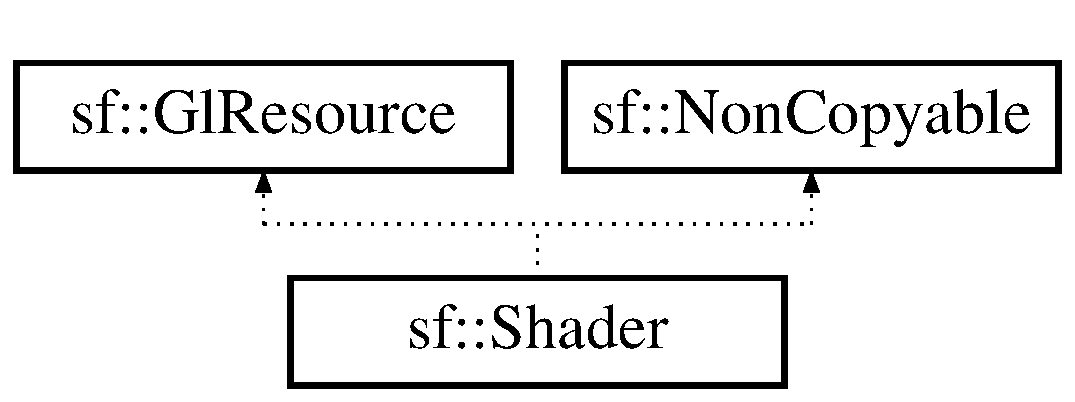
\includegraphics[height=2.000000cm]{classsf_1_1Shader}
\end{center}
\end{figure}
\subsection*{Classes}
\begin{DoxyCompactItemize}
\item 
struct \hyperlink{structsf_1_1Shader_1_1CurrentTextureType}{Current\-Texture\-Type}
\begin{DoxyCompactList}\small\item\em Special type/value that can be passed to set\-Parameter, and that represents the texture of the object being drawn. \end{DoxyCompactList}\end{DoxyCompactItemize}
\subsection*{Public Types}
\begin{DoxyCompactItemize}
\item 
enum \hyperlink{classsf_1_1Shader_afaa1aa65e5de37b74d047da9def9f9b3}{Type} \{ \hyperlink{classsf_1_1Shader_afaa1aa65e5de37b74d047da9def9f9b3a8718008f827eb32e29bbdd1791c62dce}{Vertex}, 
\hyperlink{classsf_1_1Shader_afaa1aa65e5de37b74d047da9def9f9b3ace6e88eec3a56b2e55ee3c8e64e9b89a}{Fragment}
 \}
\begin{DoxyCompactList}\small\item\em Types of shaders. \end{DoxyCompactList}\end{DoxyCompactItemize}
\subsection*{Public Member Functions}
\begin{DoxyCompactItemize}
\item 
\hyperlink{classsf_1_1Shader_a1d7f28f26b4122959fcafec871c2c3c5}{Shader} ()
\begin{DoxyCompactList}\small\item\em Default constructor. \end{DoxyCompactList}\item 
\hypertarget{classsf_1_1Shader_a4bac6cc8b046ecd8fb967c145a2380e6}{\hyperlink{classsf_1_1Shader_a4bac6cc8b046ecd8fb967c145a2380e6}{$\sim$\-Shader} ()}\label{classsf_1_1Shader_a4bac6cc8b046ecd8fb967c145a2380e6}

\begin{DoxyCompactList}\small\item\em Destructor. \end{DoxyCompactList}\item 
bool \hyperlink{classsf_1_1Shader_a053a5632848ebaca2fcd8ba29abe9e6e}{load\-From\-File} (const std\-::string \&filename, \hyperlink{classsf_1_1Shader_afaa1aa65e5de37b74d047da9def9f9b3}{Type} type)
\begin{DoxyCompactList}\small\item\em Load either the vertex or fragment shader from a file. \end{DoxyCompactList}\item 
bool \hyperlink{classsf_1_1Shader_ac9d7289966fcef562eeb92271c03e3dc}{load\-From\-File} (const std\-::string \&vertex\-Shader\-Filename, const std\-::string \&fragment\-Shader\-Filename)
\begin{DoxyCompactList}\small\item\em Load both the vertex and fragment shaders from files. \end{DoxyCompactList}\item 
bool \hyperlink{classsf_1_1Shader_ac92d46bf71dff2d791117e4e472148aa}{load\-From\-Memory} (const std\-::string \&shader, \hyperlink{classsf_1_1Shader_afaa1aa65e5de37b74d047da9def9f9b3}{Type} type)
\begin{DoxyCompactList}\small\item\em Load either the vertex or fragment shader from a source code in memory. \end{DoxyCompactList}\item 
bool \hyperlink{classsf_1_1Shader_ae34e94070d7547a890166b7993658a9b}{load\-From\-Memory} (const std\-::string \&vertex\-Shader, const std\-::string \&fragment\-Shader)
\begin{DoxyCompactList}\small\item\em Load both the vertex and fragment shaders from source codes in memory. \end{DoxyCompactList}\item 
bool \hyperlink{classsf_1_1Shader_a2ee1b130c0606e4f8bcdf65c1efc2a53}{load\-From\-Stream} (\hyperlink{classsf_1_1InputStream}{Input\-Stream} \&stream, \hyperlink{classsf_1_1Shader_afaa1aa65e5de37b74d047da9def9f9b3}{Type} type)
\begin{DoxyCompactList}\small\item\em Load either the vertex or fragment shader from a custom stream. \end{DoxyCompactList}\item 
bool \hyperlink{classsf_1_1Shader_a3b7958159ffb5596c4babc3052e35465}{load\-From\-Stream} (\hyperlink{classsf_1_1InputStream}{Input\-Stream} \&vertex\-Shader\-Stream, \hyperlink{classsf_1_1InputStream}{Input\-Stream} \&fragment\-Shader\-Stream)
\begin{DoxyCompactList}\small\item\em Load both the vertex and fragment shaders from custom streams. \end{DoxyCompactList}\item 
void \hyperlink{classsf_1_1Shader_a47e4dd78f0752ae08664b4ee616db1cf}{set\-Parameter} (const std\-::string \&name, float x)
\begin{DoxyCompactList}\small\item\em Change a float parameter of the shader. \end{DoxyCompactList}\item 
void \hyperlink{classsf_1_1Shader_ab8d379f40810b8e3eadebee81aedd231}{set\-Parameter} (const std\-::string \&name, float x, float y)
\begin{DoxyCompactList}\small\item\em Change a 2-\/components vector parameter of the shader. \end{DoxyCompactList}\item 
void \hyperlink{classsf_1_1Shader_a7e36e044d6b8adca8339f40c5a4b1801}{set\-Parameter} (const std\-::string \&name, float x, float y, float z)
\begin{DoxyCompactList}\small\item\em Change a 3-\/components vector parameter of the shader. \end{DoxyCompactList}\item 
void \hyperlink{classsf_1_1Shader_aeb468f1bc2d26750b96b74f1e19027fb}{set\-Parameter} (const std\-::string \&name, float x, float y, float z, float w)
\begin{DoxyCompactList}\small\item\em Change a 4-\/components vector parameter of the shader. \end{DoxyCompactList}\item 
void \hyperlink{classsf_1_1Shader_a3ac473ece2c6fa26dc5032c07fd7288e}{set\-Parameter} (const std\-::string \&name, const \hyperlink{classsf_1_1Vector2}{Vector2f} \&vector)
\begin{DoxyCompactList}\small\item\em Change a 2-\/components vector parameter of the shader. \end{DoxyCompactList}\item 
void \hyperlink{classsf_1_1Shader_a87d4a0c6dc70ae68aecc0dda3f343c07}{set\-Parameter} (const std\-::string \&name, const \hyperlink{classsf_1_1Vector3}{Vector3f} \&vector)
\begin{DoxyCompactList}\small\item\em Change a 3-\/components vector parameter of the shader. \end{DoxyCompactList}\item 
void \hyperlink{classsf_1_1Shader_aa8618119ed4399df3fd33e78ee96b4fc}{set\-Parameter} (const std\-::string \&name, const \hyperlink{classsf_1_1Color}{Color} \&color)
\begin{DoxyCompactList}\small\item\em Change a color parameter of the shader. \end{DoxyCompactList}\item 
void \hyperlink{classsf_1_1Shader_a39c387cc30e249b22a0c478703b8cc9a}{set\-Parameter} (const std\-::string \&name, const \hyperlink{classsf_1_1Transform}{sf\-::\-Transform} \&transform)
\begin{DoxyCompactList}\small\item\em Change a matrix parameter of the shader. \end{DoxyCompactList}\item 
void \hyperlink{classsf_1_1Shader_a7f58ab5c0a1084f238dfcec86602daa1}{set\-Parameter} (const std\-::string \&name, const \hyperlink{classsf_1_1Texture}{Texture} \&texture)
\begin{DoxyCompactList}\small\item\em Change a texture parameter of the shader. \end{DoxyCompactList}\item 
void \hyperlink{classsf_1_1Shader_af06b4cba0bab915fa01032b063909044}{set\-Parameter} (const std\-::string \&name, \hyperlink{structsf_1_1Shader_1_1CurrentTextureType}{Current\-Texture\-Type})
\begin{DoxyCompactList}\small\item\em Change a texture parameter of the shader. \end{DoxyCompactList}\end{DoxyCompactItemize}
\subsection*{Static Public Member Functions}
\begin{DoxyCompactItemize}
\item 
static void \hyperlink{classsf_1_1Shader_a09778f78afcbeb854d608c8dacd8ea30}{bind} (const \hyperlink{classsf_1_1Shader}{Shader} $\ast$shader)
\begin{DoxyCompactList}\small\item\em Bind a shader for rendering. \end{DoxyCompactList}\item 
static bool \hyperlink{classsf_1_1Shader_ad22474690bafe4a305c1b9826b1bd86a}{is\-Available} ()
\begin{DoxyCompactList}\small\item\em Tell whether or not the system supports shaders. \end{DoxyCompactList}\end{DoxyCompactItemize}
\subsection*{Static Public Attributes}
\begin{DoxyCompactItemize}
\item 
\hypertarget{classsf_1_1Shader_ac84c7953eec2e19358ea6e2cc5385b8d}{static \hyperlink{structsf_1_1Shader_1_1CurrentTextureType}{Current\-Texture\-Type} {\bfseries Current\-Texture}}\label{classsf_1_1Shader_ac84c7953eec2e19358ea6e2cc5385b8d}

\end{DoxyCompactItemize}


\subsection{Detailed Description}
\hyperlink{classsf_1_1Shader}{Shader} class (vertex and fragment) 

Shaders are programs written using a specific language, executed directly by the graphics card and allowing to apply real-\/time operations to the rendered entities.

There are two kinds of shaders\-: \begin{DoxyItemize}
\item \hyperlink{classsf_1_1Vertex}{Vertex} shaders, that process vertices \item Fragment (pixel) shaders, that process pixels\end{DoxyItemize}
A \hyperlink{classsf_1_1Shader}{sf\-::\-Shader} can be composed of either a vertex shader alone, a fragment shader alone, or both combined (see the variants of the load functions).

Shaders are written in G\-L\-S\-L, which is a C-\/like language dedicated to Open\-G\-L shaders. You'll probably need to learn its basics before writing your own shaders for S\-F\-M\-L.

Like any C/\-C++ program, a shader has its own variables that you can set from your C++ application. \hyperlink{classsf_1_1Shader}{sf\-::\-Shader} handles 5 different types of variables\-: \begin{DoxyItemize}
\item floats \item vectors (2, 3 or 4 components) \item colors \item textures \item transforms (matrices)\end{DoxyItemize}
The value of the variables can be changed at any time with the various overloads of the set\-Parameter function\-: 
\begin{DoxyCode}
shader.setParameter(\textcolor{stringliteral}{"offset"}, 2.f);
shader.setParameter(\textcolor{stringliteral}{"point"}, 0.5f, 0.8f, 0.3f);
shader.setParameter(\textcolor{stringliteral}{"color"}, \hyperlink{classsf_1_1Color}{sf::Color}(128, 50, 255));
shader.setParameter(\textcolor{stringliteral}{"matrix"}, transform); \textcolor{comment}{// transform is a sf::Transform}
shader.setParameter(\textcolor{stringliteral}{"overlay"}, texture); \textcolor{comment}{// texture is a sf::Texture}
shader.setParameter(\textcolor{stringliteral}{"texture"}, sf::Shader::CurrentTexture);
\end{DoxyCode}


The special Shader\-::\-Current\-Texture argument maps the given texture variable to the current texture of the object being drawn (which cannot be known in advance).

To apply a shader to a drawable, you must pass it as an additional parameter to the Draw function\-: 
\begin{DoxyCode}
window.draw(sprite, &shader);
\end{DoxyCode}


... which is in fact just a shortcut for this\-: 
\begin{DoxyCode}
\hyperlink{classsf_1_1RenderStates}{sf::RenderStates} states;
states.\hyperlink{classsf_1_1RenderStates_ad4f79ecdd0c60ed0d24fbe555b221bd8}{shader} = &shader;
window.draw(sprite, states);
\end{DoxyCode}


In the code above we pass a pointer to the shader, because it may be null (which means \char`\"{}no shader\char`\"{}).

Shaders can be used on any drawable, but some combinations are not interesting. For example, using a vertex shader on a \hyperlink{classsf_1_1Sprite}{sf\-::\-Sprite} is limited because there are only 4 vertices, the sprite would have to be subdivided in order to apply wave effects. Another bad example is a fragment shader with \hyperlink{classsf_1_1Text}{sf\-::\-Text}\-: the texture of the text is not the actual text that you see on screen, it is a big texture containing all the characters of the font in an arbitrary order; thus, texture lookups on pixels other than the current one may not give you the expected result.

Shaders can also be used to apply global post-\/effects to the current contents of the target (like the old sf\-::\-Post\-Fx class in S\-F\-M\-L 1). This can be done in two different ways\-: \begin{DoxyItemize}
\item draw everything to a \hyperlink{classsf_1_1RenderTexture}{sf\-::\-Render\-Texture}, then draw it to the main target using the shader \item draw everything directly to the main target, then use sf\-::\-Texture\-::update(\-Window\&) to copy its contents to a texture and draw it to the main target using the shader\end{DoxyItemize}
The first technique is more optimized because it doesn't involve retrieving the target's pixels to system memory, but the second one doesn't impact the rendering process and can be easily inserted anywhere without impacting all the code.

Like \hyperlink{classsf_1_1Texture}{sf\-::\-Texture} that can be used as a raw Open\-G\-L texture, \hyperlink{classsf_1_1Shader}{sf\-::\-Shader} can also be used directly as a raw shader for custom Open\-G\-L geometry. 
\begin{DoxyCode}
\hyperlink{classsf_1_1Shader_a09778f78afcbeb854d608c8dacd8ea30}{sf::Shader::bind}(&shader);
... render OpenGL geometry ...
sf::Shader::bind(NULL);
\end{DoxyCode}
 

Definition at line 51 of file Shader.\-hpp.



\subsection{Member Enumeration Documentation}
\hypertarget{classsf_1_1Shader_afaa1aa65e5de37b74d047da9def9f9b3}{\index{sf\-::\-Shader@{sf\-::\-Shader}!Type@{Type}}
\index{Type@{Type}!sf::Shader@{sf\-::\-Shader}}
\subsubsection[{Type}]{\setlength{\rightskip}{0pt plus 5cm}enum {\bf sf\-::\-Shader\-::\-Type}}}\label{classsf_1_1Shader_afaa1aa65e5de37b74d047da9def9f9b3}


Types of shaders. 

\begin{Desc}
\item[Enumerator]\par
\begin{description}
\index{Vertex@{Vertex}!sf\-::\-Shader@{sf\-::\-Shader}}\index{sf\-::\-Shader@{sf\-::\-Shader}!Vertex@{Vertex}}\item[{\em 
\hypertarget{classsf_1_1Shader_afaa1aa65e5de37b74d047da9def9f9b3a8718008f827eb32e29bbdd1791c62dce}{Vertex}\label{classsf_1_1Shader_afaa1aa65e5de37b74d047da9def9f9b3a8718008f827eb32e29bbdd1791c62dce}
}]\hyperlink{classsf_1_1Vertex}{Vertex} shader. \index{Fragment@{Fragment}!sf\-::\-Shader@{sf\-::\-Shader}}\index{sf\-::\-Shader@{sf\-::\-Shader}!Fragment@{Fragment}}\item[{\em 
\hypertarget{classsf_1_1Shader_afaa1aa65e5de37b74d047da9def9f9b3ace6e88eec3a56b2e55ee3c8e64e9b89a}{Fragment}\label{classsf_1_1Shader_afaa1aa65e5de37b74d047da9def9f9b3ace6e88eec3a56b2e55ee3c8e64e9b89a}
}]Fragment (pixel) shader. \end{description}
\end{Desc}


Definition at line 59 of file Shader.\-hpp.



\subsection{Constructor \& Destructor Documentation}
\hypertarget{classsf_1_1Shader_a1d7f28f26b4122959fcafec871c2c3c5}{\index{sf\-::\-Shader@{sf\-::\-Shader}!Shader@{Shader}}
\index{Shader@{Shader}!sf::Shader@{sf\-::\-Shader}}
\subsubsection[{Shader}]{\setlength{\rightskip}{0pt plus 5cm}sf\-::\-Shader\-::\-Shader (
\begin{DoxyParamCaption}
{}
\end{DoxyParamCaption}
)}}\label{classsf_1_1Shader_a1d7f28f26b4122959fcafec871c2c3c5}


Default constructor. 

This constructor creates an invalid shader. 

\subsection{Member Function Documentation}
\hypertarget{classsf_1_1Shader_a09778f78afcbeb854d608c8dacd8ea30}{\index{sf\-::\-Shader@{sf\-::\-Shader}!bind@{bind}}
\index{bind@{bind}!sf::Shader@{sf\-::\-Shader}}
\subsubsection[{bind}]{\setlength{\rightskip}{0pt plus 5cm}static void sf\-::\-Shader\-::bind (
\begin{DoxyParamCaption}
\item[{const {\bf Shader} $\ast$}]{shader}
\end{DoxyParamCaption}
)\hspace{0.3cm}{\ttfamily [static]}}}\label{classsf_1_1Shader_a09778f78afcbeb854d608c8dacd8ea30}


Bind a shader for rendering. 

This function is not part of the graphics A\-P\-I, it mustn't be used when drawing S\-F\-M\-L entities. It must be used only if you mix \hyperlink{classsf_1_1Shader}{sf\-::\-Shader} with Open\-G\-L code.


\begin{DoxyCode}
\hyperlink{classsf_1_1Shader}{sf::Shader} s1, s2;
...
sf::Shader::bind(&s1);
\textcolor{comment}{// draw OpenGL stuff that use s1...}
\hyperlink{classsf_1_1Shader_a09778f78afcbeb854d608c8dacd8ea30}{sf::Shader::bind}(&s2);
\textcolor{comment}{// draw OpenGL stuff that use s2...}
\hyperlink{classsf_1_1Shader_a09778f78afcbeb854d608c8dacd8ea30}{sf::Shader::bind}(NULL);
\textcolor{comment}{// draw OpenGL stuff that use no shader...}
\end{DoxyCode}



\begin{DoxyParams}{Parameters}
{\em shader} & \hyperlink{classsf_1_1Shader}{Shader} to bind, can be null to use no shader \\
\hline
\end{DoxyParams}
\hypertarget{classsf_1_1Shader_ad22474690bafe4a305c1b9826b1bd86a}{\index{sf\-::\-Shader@{sf\-::\-Shader}!is\-Available@{is\-Available}}
\index{is\-Available@{is\-Available}!sf::Shader@{sf\-::\-Shader}}
\subsubsection[{is\-Available}]{\setlength{\rightskip}{0pt plus 5cm}static bool sf\-::\-Shader\-::is\-Available (
\begin{DoxyParamCaption}
{}
\end{DoxyParamCaption}
)\hspace{0.3cm}{\ttfamily [static]}}}\label{classsf_1_1Shader_ad22474690bafe4a305c1b9826b1bd86a}


Tell whether or not the system supports shaders. 

This function should always be called before using the shader features. If it returns false, then any attempt to use \hyperlink{classsf_1_1Shader}{sf\-::\-Shader} will fail.

\begin{DoxyReturn}{Returns}
True if shaders are supported, false otherwise 
\end{DoxyReturn}
\hypertarget{classsf_1_1Shader_a053a5632848ebaca2fcd8ba29abe9e6e}{\index{sf\-::\-Shader@{sf\-::\-Shader}!load\-From\-File@{load\-From\-File}}
\index{load\-From\-File@{load\-From\-File}!sf::Shader@{sf\-::\-Shader}}
\subsubsection[{load\-From\-File}]{\setlength{\rightskip}{0pt plus 5cm}bool sf\-::\-Shader\-::load\-From\-File (
\begin{DoxyParamCaption}
\item[{const std\-::string \&}]{filename, }
\item[{{\bf Type}}]{type}
\end{DoxyParamCaption}
)}}\label{classsf_1_1Shader_a053a5632848ebaca2fcd8ba29abe9e6e}


Load either the vertex or fragment shader from a file. 

This function loads a single shader, either vertex or fragment, identified by the second argument. The source must be a text file containing a valid shader in G\-L\-S\-L language. G\-L\-S\-L is a C-\/like language dedicated to Open\-G\-L shaders; you'll probably need to read a good documentation for it before writing your own shaders.


\begin{DoxyParams}{Parameters}
{\em filename} & Path of the vertex or fragment shader file to load \\
\hline
{\em type} & Type of shader (vertex or fragment)\\
\hline
\end{DoxyParams}
\begin{DoxyReturn}{Returns}
True if loading succeeded, false if it failed
\end{DoxyReturn}
\begin{DoxySeeAlso}{See Also}
\hyperlink{classsf_1_1Shader_ac92d46bf71dff2d791117e4e472148aa}{load\-From\-Memory}, \hyperlink{classsf_1_1Shader_a2ee1b130c0606e4f8bcdf65c1efc2a53}{load\-From\-Stream} 
\end{DoxySeeAlso}
\hypertarget{classsf_1_1Shader_ac9d7289966fcef562eeb92271c03e3dc}{\index{sf\-::\-Shader@{sf\-::\-Shader}!load\-From\-File@{load\-From\-File}}
\index{load\-From\-File@{load\-From\-File}!sf::Shader@{sf\-::\-Shader}}
\subsubsection[{load\-From\-File}]{\setlength{\rightskip}{0pt plus 5cm}bool sf\-::\-Shader\-::load\-From\-File (
\begin{DoxyParamCaption}
\item[{const std\-::string \&}]{vertex\-Shader\-Filename, }
\item[{const std\-::string \&}]{fragment\-Shader\-Filename}
\end{DoxyParamCaption}
)}}\label{classsf_1_1Shader_ac9d7289966fcef562eeb92271c03e3dc}


Load both the vertex and fragment shaders from files. 

This function loads both the vertex and the fragment shaders. If one of them fails to load, the shader is left empty (the valid shader is unloaded). The sources must be text files containing valid shaders in G\-L\-S\-L language. G\-L\-S\-L is a C-\/like language dedicated to Open\-G\-L shaders; you'll probably need to read a good documentation for it before writing your own shaders.


\begin{DoxyParams}{Parameters}
{\em vertex\-Shader\-Filename} & Path of the vertex shader file to load \\
\hline
{\em fragment\-Shader\-Filename} & Path of the fragment shader file to load\\
\hline
\end{DoxyParams}
\begin{DoxyReturn}{Returns}
True if loading succeeded, false if it failed
\end{DoxyReturn}
\begin{DoxySeeAlso}{See Also}
\hyperlink{classsf_1_1Shader_ac92d46bf71dff2d791117e4e472148aa}{load\-From\-Memory}, \hyperlink{classsf_1_1Shader_a2ee1b130c0606e4f8bcdf65c1efc2a53}{load\-From\-Stream} 
\end{DoxySeeAlso}
\hypertarget{classsf_1_1Shader_ac92d46bf71dff2d791117e4e472148aa}{\index{sf\-::\-Shader@{sf\-::\-Shader}!load\-From\-Memory@{load\-From\-Memory}}
\index{load\-From\-Memory@{load\-From\-Memory}!sf::Shader@{sf\-::\-Shader}}
\subsubsection[{load\-From\-Memory}]{\setlength{\rightskip}{0pt plus 5cm}bool sf\-::\-Shader\-::load\-From\-Memory (
\begin{DoxyParamCaption}
\item[{const std\-::string \&}]{shader, }
\item[{{\bf Type}}]{type}
\end{DoxyParamCaption}
)}}\label{classsf_1_1Shader_ac92d46bf71dff2d791117e4e472148aa}


Load either the vertex or fragment shader from a source code in memory. 

This function loads a single shader, either vertex or fragment, identified by the second argument. The source code must be a valid shader in G\-L\-S\-L language. G\-L\-S\-L is a C-\/like language dedicated to Open\-G\-L shaders; you'll probably need to read a good documentation for it before writing your own shaders.


\begin{DoxyParams}{Parameters}
{\em shader} & \hyperlink{classsf_1_1String}{String} containing the source code of the shader \\
\hline
{\em type} & Type of shader (vertex or fragment)\\
\hline
\end{DoxyParams}
\begin{DoxyReturn}{Returns}
True if loading succeeded, false if it failed
\end{DoxyReturn}
\begin{DoxySeeAlso}{See Also}
\hyperlink{classsf_1_1Shader_a053a5632848ebaca2fcd8ba29abe9e6e}{load\-From\-File}, \hyperlink{classsf_1_1Shader_a2ee1b130c0606e4f8bcdf65c1efc2a53}{load\-From\-Stream} 
\end{DoxySeeAlso}
\hypertarget{classsf_1_1Shader_ae34e94070d7547a890166b7993658a9b}{\index{sf\-::\-Shader@{sf\-::\-Shader}!load\-From\-Memory@{load\-From\-Memory}}
\index{load\-From\-Memory@{load\-From\-Memory}!sf::Shader@{sf\-::\-Shader}}
\subsubsection[{load\-From\-Memory}]{\setlength{\rightskip}{0pt plus 5cm}bool sf\-::\-Shader\-::load\-From\-Memory (
\begin{DoxyParamCaption}
\item[{const std\-::string \&}]{vertex\-Shader, }
\item[{const std\-::string \&}]{fragment\-Shader}
\end{DoxyParamCaption}
)}}\label{classsf_1_1Shader_ae34e94070d7547a890166b7993658a9b}


Load both the vertex and fragment shaders from source codes in memory. 

This function loads both the vertex and the fragment shaders. If one of them fails to load, the shader is left empty (the valid shader is unloaded). The sources must be valid shaders in G\-L\-S\-L language. G\-L\-S\-L is a C-\/like language dedicated to Open\-G\-L shaders; you'll probably need to read a good documentation for it before writing your own shaders.


\begin{DoxyParams}{Parameters}
{\em vertex\-Shader} & \hyperlink{classsf_1_1String}{String} containing the source code of the vertex shader \\
\hline
{\em fragment\-Shader} & \hyperlink{classsf_1_1String}{String} containing the source code of the fragment shader\\
\hline
\end{DoxyParams}
\begin{DoxyReturn}{Returns}
True if loading succeeded, false if it failed
\end{DoxyReturn}
\begin{DoxySeeAlso}{See Also}
\hyperlink{classsf_1_1Shader_a053a5632848ebaca2fcd8ba29abe9e6e}{load\-From\-File}, \hyperlink{classsf_1_1Shader_a2ee1b130c0606e4f8bcdf65c1efc2a53}{load\-From\-Stream} 
\end{DoxySeeAlso}
\hypertarget{classsf_1_1Shader_a2ee1b130c0606e4f8bcdf65c1efc2a53}{\index{sf\-::\-Shader@{sf\-::\-Shader}!load\-From\-Stream@{load\-From\-Stream}}
\index{load\-From\-Stream@{load\-From\-Stream}!sf::Shader@{sf\-::\-Shader}}
\subsubsection[{load\-From\-Stream}]{\setlength{\rightskip}{0pt plus 5cm}bool sf\-::\-Shader\-::load\-From\-Stream (
\begin{DoxyParamCaption}
\item[{{\bf Input\-Stream} \&}]{stream, }
\item[{{\bf Type}}]{type}
\end{DoxyParamCaption}
)}}\label{classsf_1_1Shader_a2ee1b130c0606e4f8bcdf65c1efc2a53}


Load either the vertex or fragment shader from a custom stream. 

This function loads a single shader, either vertex or fragment, identified by the second argument. The source code must be a valid shader in G\-L\-S\-L language. G\-L\-S\-L is a C-\/like language dedicated to Open\-G\-L shaders; you'll probably need to read a good documentation for it before writing your own shaders.


\begin{DoxyParams}{Parameters}
{\em stream} & Source stream to read from \\
\hline
{\em type} & Type of shader (vertex or fragment)\\
\hline
\end{DoxyParams}
\begin{DoxyReturn}{Returns}
True if loading succeeded, false if it failed
\end{DoxyReturn}
\begin{DoxySeeAlso}{See Also}
\hyperlink{classsf_1_1Shader_a053a5632848ebaca2fcd8ba29abe9e6e}{load\-From\-File}, \hyperlink{classsf_1_1Shader_ac92d46bf71dff2d791117e4e472148aa}{load\-From\-Memory} 
\end{DoxySeeAlso}
\hypertarget{classsf_1_1Shader_a3b7958159ffb5596c4babc3052e35465}{\index{sf\-::\-Shader@{sf\-::\-Shader}!load\-From\-Stream@{load\-From\-Stream}}
\index{load\-From\-Stream@{load\-From\-Stream}!sf::Shader@{sf\-::\-Shader}}
\subsubsection[{load\-From\-Stream}]{\setlength{\rightskip}{0pt plus 5cm}bool sf\-::\-Shader\-::load\-From\-Stream (
\begin{DoxyParamCaption}
\item[{{\bf Input\-Stream} \&}]{vertex\-Shader\-Stream, }
\item[{{\bf Input\-Stream} \&}]{fragment\-Shader\-Stream}
\end{DoxyParamCaption}
)}}\label{classsf_1_1Shader_a3b7958159ffb5596c4babc3052e35465}


Load both the vertex and fragment shaders from custom streams. 

This function loads both the vertex and the fragment shaders. If one of them fails to load, the shader is left empty (the valid shader is unloaded). The source codes must be valid shaders in G\-L\-S\-L language. G\-L\-S\-L is a C-\/like language dedicated to Open\-G\-L shaders; you'll probably need to read a good documentation for it before writing your own shaders.


\begin{DoxyParams}{Parameters}
{\em vertex\-Shader\-Stream} & Source stream to read the vertex shader from \\
\hline
{\em fragment\-Shader\-Stream} & Source stream to read the fragment shader from\\
\hline
\end{DoxyParams}
\begin{DoxyReturn}{Returns}
True if loading succeeded, false if it failed
\end{DoxyReturn}
\begin{DoxySeeAlso}{See Also}
\hyperlink{classsf_1_1Shader_a053a5632848ebaca2fcd8ba29abe9e6e}{load\-From\-File}, \hyperlink{classsf_1_1Shader_ac92d46bf71dff2d791117e4e472148aa}{load\-From\-Memory} 
\end{DoxySeeAlso}
\hypertarget{classsf_1_1Shader_a47e4dd78f0752ae08664b4ee616db1cf}{\index{sf\-::\-Shader@{sf\-::\-Shader}!set\-Parameter@{set\-Parameter}}
\index{set\-Parameter@{set\-Parameter}!sf::Shader@{sf\-::\-Shader}}
\subsubsection[{set\-Parameter}]{\setlength{\rightskip}{0pt plus 5cm}void sf\-::\-Shader\-::set\-Parameter (
\begin{DoxyParamCaption}
\item[{const std\-::string \&}]{name, }
\item[{float}]{x}
\end{DoxyParamCaption}
)}}\label{classsf_1_1Shader_a47e4dd78f0752ae08664b4ee616db1cf}


Change a float parameter of the shader. 

{\itshape name} is the name of the variable to change in the shader. The corresponding parameter in the shader must be a float (float G\-L\-S\-L type).

Example\-: 
\begin{DoxyCode}
uniform \textcolor{keywordtype}{float} myparam; \textcolor{comment}{// this is the variable in the shader}
\end{DoxyCode}
 
\begin{DoxyCode}
shader.setParameter(\textcolor{stringliteral}{"myparam"}, 5.2f);
\end{DoxyCode}



\begin{DoxyParams}{Parameters}
{\em name} & Name of the parameter in the shader \\
\hline
{\em x} & Value to assign \\
\hline
\end{DoxyParams}
\hypertarget{classsf_1_1Shader_ab8d379f40810b8e3eadebee81aedd231}{\index{sf\-::\-Shader@{sf\-::\-Shader}!set\-Parameter@{set\-Parameter}}
\index{set\-Parameter@{set\-Parameter}!sf::Shader@{sf\-::\-Shader}}
\subsubsection[{set\-Parameter}]{\setlength{\rightskip}{0pt plus 5cm}void sf\-::\-Shader\-::set\-Parameter (
\begin{DoxyParamCaption}
\item[{const std\-::string \&}]{name, }
\item[{float}]{x, }
\item[{float}]{y}
\end{DoxyParamCaption}
)}}\label{classsf_1_1Shader_ab8d379f40810b8e3eadebee81aedd231}


Change a 2-\/components vector parameter of the shader. 

{\itshape name} is the name of the variable to change in the shader. The corresponding parameter in the shader must be a 2x1 vector (vec2 G\-L\-S\-L type).

Example\-: 
\begin{DoxyCode}
uniform vec2 myparam; \textcolor{comment}{// this is the variable in the shader}
\end{DoxyCode}
 
\begin{DoxyCode}
shader.setParameter(\textcolor{stringliteral}{"myparam"}, 5.2f, 6.0f);
\end{DoxyCode}



\begin{DoxyParams}{Parameters}
{\em name} & Name of the parameter in the shader \\
\hline
{\em x} & First component of the value to assign \\
\hline
{\em y} & Second component of the value to assign \\
\hline
\end{DoxyParams}
\hypertarget{classsf_1_1Shader_a7e36e044d6b8adca8339f40c5a4b1801}{\index{sf\-::\-Shader@{sf\-::\-Shader}!set\-Parameter@{set\-Parameter}}
\index{set\-Parameter@{set\-Parameter}!sf::Shader@{sf\-::\-Shader}}
\subsubsection[{set\-Parameter}]{\setlength{\rightskip}{0pt plus 5cm}void sf\-::\-Shader\-::set\-Parameter (
\begin{DoxyParamCaption}
\item[{const std\-::string \&}]{name, }
\item[{float}]{x, }
\item[{float}]{y, }
\item[{float}]{z}
\end{DoxyParamCaption}
)}}\label{classsf_1_1Shader_a7e36e044d6b8adca8339f40c5a4b1801}


Change a 3-\/components vector parameter of the shader. 

{\itshape name} is the name of the variable to change in the shader. The corresponding parameter in the shader must be a 3x1 vector (vec3 G\-L\-S\-L type).

Example\-: 
\begin{DoxyCode}
uniform vec3 myparam; \textcolor{comment}{// this is the variable in the shader}
\end{DoxyCode}
 
\begin{DoxyCode}
shader.setParameter(\textcolor{stringliteral}{"myparam"}, 5.2f, 6.0f, -8.1f);
\end{DoxyCode}



\begin{DoxyParams}{Parameters}
{\em name} & Name of the parameter in the shader \\
\hline
{\em x} & First component of the value to assign \\
\hline
{\em y} & Second component of the value to assign \\
\hline
{\em z} & Third component of the value to assign \\
\hline
\end{DoxyParams}
\hypertarget{classsf_1_1Shader_aeb468f1bc2d26750b96b74f1e19027fb}{\index{sf\-::\-Shader@{sf\-::\-Shader}!set\-Parameter@{set\-Parameter}}
\index{set\-Parameter@{set\-Parameter}!sf::Shader@{sf\-::\-Shader}}
\subsubsection[{set\-Parameter}]{\setlength{\rightskip}{0pt plus 5cm}void sf\-::\-Shader\-::set\-Parameter (
\begin{DoxyParamCaption}
\item[{const std\-::string \&}]{name, }
\item[{float}]{x, }
\item[{float}]{y, }
\item[{float}]{z, }
\item[{float}]{w}
\end{DoxyParamCaption}
)}}\label{classsf_1_1Shader_aeb468f1bc2d26750b96b74f1e19027fb}


Change a 4-\/components vector parameter of the shader. 

{\itshape name} is the name of the variable to change in the shader. The corresponding parameter in the shader must be a 4x1 vector (vec4 G\-L\-S\-L type).

Example\-: 
\begin{DoxyCode}
uniform vec4 myparam; \textcolor{comment}{// this is the variable in the shader}
\end{DoxyCode}
 
\begin{DoxyCode}
shader.setParameter(\textcolor{stringliteral}{"myparam"}, 5.2f, 6.0f, -8.1f, 0.4f);
\end{DoxyCode}



\begin{DoxyParams}{Parameters}
{\em name} & Name of the parameter in the shader \\
\hline
{\em x} & First component of the value to assign \\
\hline
{\em y} & Second component of the value to assign \\
\hline
{\em z} & Third component of the value to assign \\
\hline
{\em w} & Fourth component of the value to assign \\
\hline
\end{DoxyParams}
\hypertarget{classsf_1_1Shader_a3ac473ece2c6fa26dc5032c07fd7288e}{\index{sf\-::\-Shader@{sf\-::\-Shader}!set\-Parameter@{set\-Parameter}}
\index{set\-Parameter@{set\-Parameter}!sf::Shader@{sf\-::\-Shader}}
\subsubsection[{set\-Parameter}]{\setlength{\rightskip}{0pt plus 5cm}void sf\-::\-Shader\-::set\-Parameter (
\begin{DoxyParamCaption}
\item[{const std\-::string \&}]{name, }
\item[{const {\bf Vector2f} \&}]{vector}
\end{DoxyParamCaption}
)}}\label{classsf_1_1Shader_a3ac473ece2c6fa26dc5032c07fd7288e}


Change a 2-\/components vector parameter of the shader. 

{\itshape name} is the name of the variable to change in the shader. The corresponding parameter in the shader must be a 2x1 vector (vec2 G\-L\-S\-L type).

Example\-: 
\begin{DoxyCode}
uniform vec2 myparam; \textcolor{comment}{// this is the variable in the shader}
\end{DoxyCode}
 
\begin{DoxyCode}
shader.setParameter(\textcolor{stringliteral}{"myparam"}, \hyperlink{classsf_1_1Vector2}{sf::Vector2f}(5.2f, 6.0f));
\end{DoxyCode}



\begin{DoxyParams}{Parameters}
{\em name} & Name of the parameter in the shader \\
\hline
{\em vector} & Vector to assign \\
\hline
\end{DoxyParams}
\hypertarget{classsf_1_1Shader_a87d4a0c6dc70ae68aecc0dda3f343c07}{\index{sf\-::\-Shader@{sf\-::\-Shader}!set\-Parameter@{set\-Parameter}}
\index{set\-Parameter@{set\-Parameter}!sf::Shader@{sf\-::\-Shader}}
\subsubsection[{set\-Parameter}]{\setlength{\rightskip}{0pt plus 5cm}void sf\-::\-Shader\-::set\-Parameter (
\begin{DoxyParamCaption}
\item[{const std\-::string \&}]{name, }
\item[{const {\bf Vector3f} \&}]{vector}
\end{DoxyParamCaption}
)}}\label{classsf_1_1Shader_a87d4a0c6dc70ae68aecc0dda3f343c07}


Change a 3-\/components vector parameter of the shader. 

{\itshape name} is the name of the variable to change in the shader. The corresponding parameter in the shader must be a 3x1 vector (vec3 G\-L\-S\-L type).

Example\-: 
\begin{DoxyCode}
uniform vec3 myparam; \textcolor{comment}{// this is the variable in the shader}
\end{DoxyCode}
 
\begin{DoxyCode}
shader.setParameter(\textcolor{stringliteral}{"myparam"}, \hyperlink{classsf_1_1Vector3}{sf::Vector3f}(5.2f, 6.0f, -8.1f));
\end{DoxyCode}



\begin{DoxyParams}{Parameters}
{\em name} & Name of the parameter in the shader \\
\hline
{\em vector} & Vector to assign \\
\hline
\end{DoxyParams}
\hypertarget{classsf_1_1Shader_aa8618119ed4399df3fd33e78ee96b4fc}{\index{sf\-::\-Shader@{sf\-::\-Shader}!set\-Parameter@{set\-Parameter}}
\index{set\-Parameter@{set\-Parameter}!sf::Shader@{sf\-::\-Shader}}
\subsubsection[{set\-Parameter}]{\setlength{\rightskip}{0pt plus 5cm}void sf\-::\-Shader\-::set\-Parameter (
\begin{DoxyParamCaption}
\item[{const std\-::string \&}]{name, }
\item[{const {\bf Color} \&}]{color}
\end{DoxyParamCaption}
)}}\label{classsf_1_1Shader_aa8618119ed4399df3fd33e78ee96b4fc}


Change a color parameter of the shader. 

{\itshape name} is the name of the variable to change in the shader. The corresponding parameter in the shader must be a 4x1 vector (vec4 G\-L\-S\-L type).

It is important to note that the components of the color are normalized before being passed to the shader. Therefore, they are converted from range \mbox{[}0 .. 255\mbox{]} to range \mbox{[}0 .. 1\mbox{]}. For example, a \hyperlink{classsf_1_1Color}{sf\-::\-Color(255, 125, 0, 255)} will be transformed to a vec4(1.\-0, 0.\-5, 0.\-0, 1.\-0) in the shader.

Example\-: 
\begin{DoxyCode}
uniform vec4 color; \textcolor{comment}{// this is the variable in the shader}
\end{DoxyCode}
 
\begin{DoxyCode}
shader.setParameter(\textcolor{stringliteral}{"color"}, \hyperlink{classsf_1_1Color}{sf::Color}(255, 128, 0, 255));
\end{DoxyCode}



\begin{DoxyParams}{Parameters}
{\em name} & Name of the parameter in the shader \\
\hline
{\em color} & \hyperlink{classsf_1_1Color}{Color} to assign \\
\hline
\end{DoxyParams}
\hypertarget{classsf_1_1Shader_a39c387cc30e249b22a0c478703b8cc9a}{\index{sf\-::\-Shader@{sf\-::\-Shader}!set\-Parameter@{set\-Parameter}}
\index{set\-Parameter@{set\-Parameter}!sf::Shader@{sf\-::\-Shader}}
\subsubsection[{set\-Parameter}]{\setlength{\rightskip}{0pt plus 5cm}void sf\-::\-Shader\-::set\-Parameter (
\begin{DoxyParamCaption}
\item[{const std\-::string \&}]{name, }
\item[{const {\bf sf\-::\-Transform} \&}]{transform}
\end{DoxyParamCaption}
)}}\label{classsf_1_1Shader_a39c387cc30e249b22a0c478703b8cc9a}


Change a matrix parameter of the shader. 

{\itshape name} is the name of the variable to change in the shader. The corresponding parameter in the shader must be a 4x4 matrix (mat4 G\-L\-S\-L type).

Example\-: 
\begin{DoxyCode}
uniform mat4 matrix; \textcolor{comment}{// this is the variable in the shader}
\end{DoxyCode}
 
\begin{DoxyCode}
\hyperlink{classsf_1_1Transform}{sf::Transform} transform;
transform.\hyperlink{classsf_1_1Transform_ab54f6c8070cc05e2afcb3145fbf4395a}{translate}(5, 10);
shader.setParameter(\textcolor{stringliteral}{"matrix"}, transform);
\end{DoxyCode}



\begin{DoxyParams}{Parameters}
{\em name} & Name of the parameter in the shader \\
\hline
{\em transform} & \hyperlink{classsf_1_1Transform}{Transform} to assign \\
\hline
\end{DoxyParams}
\hypertarget{classsf_1_1Shader_a7f58ab5c0a1084f238dfcec86602daa1}{\index{sf\-::\-Shader@{sf\-::\-Shader}!set\-Parameter@{set\-Parameter}}
\index{set\-Parameter@{set\-Parameter}!sf::Shader@{sf\-::\-Shader}}
\subsubsection[{set\-Parameter}]{\setlength{\rightskip}{0pt plus 5cm}void sf\-::\-Shader\-::set\-Parameter (
\begin{DoxyParamCaption}
\item[{const std\-::string \&}]{name, }
\item[{const {\bf Texture} \&}]{texture}
\end{DoxyParamCaption}
)}}\label{classsf_1_1Shader_a7f58ab5c0a1084f238dfcec86602daa1}


Change a texture parameter of the shader. 

{\itshape name} is the name of the variable to change in the shader. The corresponding parameter in the shader must be a 2\-D texture (sampler2\-D G\-L\-S\-L type).

Example\-: 
\begin{DoxyCode}
uniform sampler2D the\_texture; \textcolor{comment}{// this is the variable in the shader}
\end{DoxyCode}
 
\begin{DoxyCode}
\hyperlink{classsf_1_1Texture}{sf::Texture} texture;
...
shader.setParameter(\textcolor{stringliteral}{"the\_texture"}, texture);
\end{DoxyCode}
 It is important to note that {\itshape texture} must remain alive as long as the shader uses it, no copy is made internally.

To use the texture of the object being draw, which cannot be known in advance, you can pass the special value sf\-::\-Shader\-::\-Current\-Texture\-: 
\begin{DoxyCode}
shader.setParameter(\textcolor{stringliteral}{"the\_texture"}, sf::Shader::CurrentTexture).
\end{DoxyCode}



\begin{DoxyParams}{Parameters}
{\em name} & Name of the texture in the shader \\
\hline
{\em texture} & \hyperlink{classsf_1_1Texture}{Texture} to assign \\
\hline
\end{DoxyParams}
\hypertarget{classsf_1_1Shader_af06b4cba0bab915fa01032b063909044}{\index{sf\-::\-Shader@{sf\-::\-Shader}!set\-Parameter@{set\-Parameter}}
\index{set\-Parameter@{set\-Parameter}!sf::Shader@{sf\-::\-Shader}}
\subsubsection[{set\-Parameter}]{\setlength{\rightskip}{0pt plus 5cm}void sf\-::\-Shader\-::set\-Parameter (
\begin{DoxyParamCaption}
\item[{const std\-::string \&}]{name, }
\item[{{\bf Current\-Texture\-Type}}]{}
\end{DoxyParamCaption}
)}}\label{classsf_1_1Shader_af06b4cba0bab915fa01032b063909044}


Change a texture parameter of the shader. 

This overload maps a shader texture variable to the texture of the object being drawn, which cannot be known in advance. The second argument must be sf\-::\-Shader\-::\-Current\-Texture. The corresponding parameter in the shader must be a 2\-D texture (sampler2\-D G\-L\-S\-L type).

Example\-: 
\begin{DoxyCode}
uniform sampler2D current; \textcolor{comment}{// this is the variable in the shader}
\end{DoxyCode}
 
\begin{DoxyCode}
shader.setParameter(\textcolor{stringliteral}{"current"}, sf::Shader::CurrentTexture);
\end{DoxyCode}



\begin{DoxyParams}{Parameters}
{\em name} & Name of the texture in the shader \\
\hline
\end{DoxyParams}


The documentation for this class was generated from the following file\-:\begin{DoxyCompactItemize}
\item 
/home/z\-Zelman/\-Dropbox/\-Placeholder-\/\-R\-T\-S/\-S\-F\-M\-L-\/2.\-1/include/\-S\-F\-M\-L/\-Graphics/Shader.\-hpp\end{DoxyCompactItemize}

\hypertarget{classsf_1_1Shape}{\section{sf\-:\-:Shape Class Reference}
\label{classsf_1_1Shape}\index{sf\-::\-Shape@{sf\-::\-Shape}}
}


Base class for textured shapes with outline.  




{\ttfamily \#include $<$Shape.\-hpp$>$}

Inheritance diagram for sf\-:\-:Shape\-:\begin{figure}[H]
\begin{center}
\leavevmode
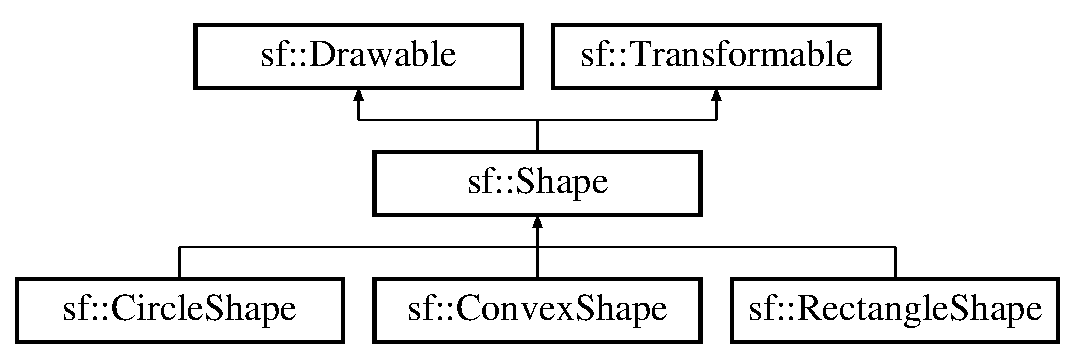
\includegraphics[height=3.000000cm]{classsf_1_1Shape}
\end{center}
\end{figure}
\subsection*{Public Member Functions}
\begin{DoxyCompactItemize}
\item 
\hypertarget{classsf_1_1Shape_a2262aceb9df52d4275c19633592f19bf}{virtual \hyperlink{classsf_1_1Shape_a2262aceb9df52d4275c19633592f19bf}{$\sim$\-Shape} ()}\label{classsf_1_1Shape_a2262aceb9df52d4275c19633592f19bf}

\begin{DoxyCompactList}\small\item\em Virtual destructor. \end{DoxyCompactList}\item 
void \hyperlink{classsf_1_1Shape_af8fb22bab1956325be5d62282711e3b6}{set\-Texture} (const \hyperlink{classsf_1_1Texture}{Texture} $\ast$texture, bool reset\-Rect=false)
\begin{DoxyCompactList}\small\item\em Change the source texture of the shape. \end{DoxyCompactList}\item 
void \hyperlink{classsf_1_1Shape_a2029cc820d1740d14ac794b82525e157}{set\-Texture\-Rect} (const \hyperlink{classsf_1_1Rect}{Int\-Rect} \&rect)
\begin{DoxyCompactList}\small\item\em Set the sub-\/rectangle of the texture that the shape will display. \end{DoxyCompactList}\item 
void \hyperlink{classsf_1_1Shape_a3506f9b5d916fec14d583d16f23c2485}{set\-Fill\-Color} (const \hyperlink{classsf_1_1Color}{Color} \&color)
\begin{DoxyCompactList}\small\item\em Set the fill color of the shape. \end{DoxyCompactList}\item 
void \hyperlink{classsf_1_1Shape_a5978f41ee349ac3c52942996dcb184f7}{set\-Outline\-Color} (const \hyperlink{classsf_1_1Color}{Color} \&color)
\begin{DoxyCompactList}\small\item\em Set the outline color of the shape. \end{DoxyCompactList}\item 
void \hyperlink{classsf_1_1Shape_a5ad336ad74fc1f567fce3b7e44cf87dc}{set\-Outline\-Thickness} (float thickness)
\begin{DoxyCompactList}\small\item\em Set the thickness of the shape's outline. \end{DoxyCompactList}\item 
const \hyperlink{classsf_1_1Texture}{Texture} $\ast$ \hyperlink{classsf_1_1Shape_a1bf27ac425fcce36efd0eed67531a403}{get\-Texture} () const 
\begin{DoxyCompactList}\small\item\em Get the source texture of the shape. \end{DoxyCompactList}\item 
const \hyperlink{classsf_1_1Rect}{Int\-Rect} \& \hyperlink{classsf_1_1Shape_af7c4c80a435b85a622812711cf510439}{get\-Texture\-Rect} () const 
\begin{DoxyCompactList}\small\item\em Get the sub-\/rectangle of the texture displayed by the shape. \end{DoxyCompactList}\item 
const \hyperlink{classsf_1_1Color}{Color} \& \hyperlink{classsf_1_1Shape_ad7f7fe601a8bb24efe9aa77809a35c12}{get\-Fill\-Color} () const 
\begin{DoxyCompactList}\small\item\em Get the fill color of the shape. \end{DoxyCompactList}\item 
const \hyperlink{classsf_1_1Color}{Color} \& \hyperlink{classsf_1_1Shape_a4fa7d3bf5ee2332f6b9d9bebe9b1e2fd}{get\-Outline\-Color} () const 
\begin{DoxyCompactList}\small\item\em Get the outline color of the shape. \end{DoxyCompactList}\item 
float \hyperlink{classsf_1_1Shape_ac66f917b41eda6159a8ba6571d77f2ad}{get\-Outline\-Thickness} () const 
\begin{DoxyCompactList}\small\item\em Get the outline thickness of the shape. \end{DoxyCompactList}\item 
virtual unsigned int \hyperlink{classsf_1_1Shape_ad84e1b675ecd270ad8151aea4e271a78}{get\-Point\-Count} () const =0
\begin{DoxyCompactList}\small\item\em Get the total number of points of the shape. \end{DoxyCompactList}\item 
virtual \hyperlink{classsf_1_1Vector2}{Vector2f} \hyperlink{classsf_1_1Shape_a397f3b4cdb7ad98cdc6c034816c652d2}{get\-Point} (unsigned int index) const =0
\begin{DoxyCompactList}\small\item\em Get a point of the shape. \end{DoxyCompactList}\item 
\hyperlink{classsf_1_1Rect}{Float\-Rect} \hyperlink{classsf_1_1Shape_a5d26a18ccfe850ff8d327ca97edbc34a}{get\-Local\-Bounds} () const 
\begin{DoxyCompactList}\small\item\em Get the local bounding rectangle of the entity. \end{DoxyCompactList}\item 
\hyperlink{classsf_1_1Rect}{Float\-Rect} \hyperlink{classsf_1_1Shape_a5257341fe832884dbba6b9dc855e33cc}{get\-Global\-Bounds} () const 
\begin{DoxyCompactList}\small\item\em Get the global bounding rectangle of the entity. \end{DoxyCompactList}\end{DoxyCompactItemize}
\subsection*{Protected Member Functions}
\begin{DoxyCompactItemize}
\item 
\hypertarget{classsf_1_1Shape_a413a457f720835b9f5d8e97ca8b80960}{\hyperlink{classsf_1_1Shape_a413a457f720835b9f5d8e97ca8b80960}{Shape} ()}\label{classsf_1_1Shape_a413a457f720835b9f5d8e97ca8b80960}

\begin{DoxyCompactList}\small\item\em Default constructor. \end{DoxyCompactList}\item 
void \hyperlink{classsf_1_1Shape_adfb2bd966c8edbc5d6c92ebc375e4ac1}{update} ()
\begin{DoxyCompactList}\small\item\em Recompute the internal geometry of the shape. \end{DoxyCompactList}\end{DoxyCompactItemize}


\subsection{Detailed Description}
Base class for textured shapes with outline. 

\hyperlink{classsf_1_1Shape}{sf\-::\-Shape} is a drawable class that allows to define and display a custom convex shape on a render target. It's only an abstract base, it needs to be specialized for concrete types of shapes (circle, rectangle, convex polygon, star, ...).

In addition to the attributes provided by the specialized shape classes, a shape always has the following attributes\-: \begin{DoxyItemize}
\item a texture \item a texture rectangle \item a fill color \item an outline color \item an outline thickness\end{DoxyItemize}
Each feature is optional, and can be disabled easily\-: \begin{DoxyItemize}
\item the texture can be null \item the fill/outline colors can be \hyperlink{classsf_1_1Color_a569b45471737f770656f50ae7bbac292}{sf\-::\-Color\-::\-Transparent} \item the outline thickness can be zero\end{DoxyItemize}
You can write your own derived shape class, there are only two virtual functions to override\-: \begin{DoxyItemize}
\item get\-Point\-Count must return the number of points of the shape \item get\-Point must return the points of the shape\end{DoxyItemize}
\begin{DoxySeeAlso}{See Also}
\hyperlink{classsf_1_1RectangleShape}{sf\-::\-Rectangle\-Shape}, \hyperlink{classsf_1_1CircleShape}{sf\-::\-Circle\-Shape}, \hyperlink{classsf_1_1ConvexShape}{sf\-::\-Convex\-Shape}, \hyperlink{classsf_1_1Transformable}{sf\-::\-Transformable} 
\end{DoxySeeAlso}


Definition at line 44 of file Shape.\-hpp.



\subsection{Member Function Documentation}
\hypertarget{classsf_1_1Shape_ad7f7fe601a8bb24efe9aa77809a35c12}{\index{sf\-::\-Shape@{sf\-::\-Shape}!get\-Fill\-Color@{get\-Fill\-Color}}
\index{get\-Fill\-Color@{get\-Fill\-Color}!sf::Shape@{sf\-::\-Shape}}
\subsubsection[{get\-Fill\-Color}]{\setlength{\rightskip}{0pt plus 5cm}const {\bf Color}\& sf\-::\-Shape\-::get\-Fill\-Color (
\begin{DoxyParamCaption}
{}
\end{DoxyParamCaption}
) const}}\label{classsf_1_1Shape_ad7f7fe601a8bb24efe9aa77809a35c12}


Get the fill color of the shape. 

\begin{DoxyReturn}{Returns}
Fill color of the shape
\end{DoxyReturn}
\begin{DoxySeeAlso}{See Also}
\hyperlink{classsf_1_1Shape_a3506f9b5d916fec14d583d16f23c2485}{set\-Fill\-Color} 
\end{DoxySeeAlso}
\hypertarget{classsf_1_1Shape_a5257341fe832884dbba6b9dc855e33cc}{\index{sf\-::\-Shape@{sf\-::\-Shape}!get\-Global\-Bounds@{get\-Global\-Bounds}}
\index{get\-Global\-Bounds@{get\-Global\-Bounds}!sf::Shape@{sf\-::\-Shape}}
\subsubsection[{get\-Global\-Bounds}]{\setlength{\rightskip}{0pt plus 5cm}{\bf Float\-Rect} sf\-::\-Shape\-::get\-Global\-Bounds (
\begin{DoxyParamCaption}
{}
\end{DoxyParamCaption}
) const}}\label{classsf_1_1Shape_a5257341fe832884dbba6b9dc855e33cc}


Get the global bounding rectangle of the entity. 

The returned rectangle is in global coordinates, which means that it takes in account the transformations (translation, rotation, scale, ...) that are applied to the entity. In other words, this function returns the bounds of the sprite in the global 2\-D world's coordinate system.

\begin{DoxyReturn}{Returns}
Global bounding rectangle of the entity 
\end{DoxyReturn}
\hypertarget{classsf_1_1Shape_a5d26a18ccfe850ff8d327ca97edbc34a}{\index{sf\-::\-Shape@{sf\-::\-Shape}!get\-Local\-Bounds@{get\-Local\-Bounds}}
\index{get\-Local\-Bounds@{get\-Local\-Bounds}!sf::Shape@{sf\-::\-Shape}}
\subsubsection[{get\-Local\-Bounds}]{\setlength{\rightskip}{0pt plus 5cm}{\bf Float\-Rect} sf\-::\-Shape\-::get\-Local\-Bounds (
\begin{DoxyParamCaption}
{}
\end{DoxyParamCaption}
) const}}\label{classsf_1_1Shape_a5d26a18ccfe850ff8d327ca97edbc34a}


Get the local bounding rectangle of the entity. 

The returned rectangle is in local coordinates, which means that it ignores the transformations (translation, rotation, scale, ...) that are applied to the entity. In other words, this function returns the bounds of the entity in the entity's coordinate system.

\begin{DoxyReturn}{Returns}
Local bounding rectangle of the entity 
\end{DoxyReturn}
\hypertarget{classsf_1_1Shape_a4fa7d3bf5ee2332f6b9d9bebe9b1e2fd}{\index{sf\-::\-Shape@{sf\-::\-Shape}!get\-Outline\-Color@{get\-Outline\-Color}}
\index{get\-Outline\-Color@{get\-Outline\-Color}!sf::Shape@{sf\-::\-Shape}}
\subsubsection[{get\-Outline\-Color}]{\setlength{\rightskip}{0pt plus 5cm}const {\bf Color}\& sf\-::\-Shape\-::get\-Outline\-Color (
\begin{DoxyParamCaption}
{}
\end{DoxyParamCaption}
) const}}\label{classsf_1_1Shape_a4fa7d3bf5ee2332f6b9d9bebe9b1e2fd}


Get the outline color of the shape. 

\begin{DoxyReturn}{Returns}
Outline color of the shape
\end{DoxyReturn}
\begin{DoxySeeAlso}{See Also}
\hyperlink{classsf_1_1Shape_a5978f41ee349ac3c52942996dcb184f7}{set\-Outline\-Color} 
\end{DoxySeeAlso}
\hypertarget{classsf_1_1Shape_ac66f917b41eda6159a8ba6571d77f2ad}{\index{sf\-::\-Shape@{sf\-::\-Shape}!get\-Outline\-Thickness@{get\-Outline\-Thickness}}
\index{get\-Outline\-Thickness@{get\-Outline\-Thickness}!sf::Shape@{sf\-::\-Shape}}
\subsubsection[{get\-Outline\-Thickness}]{\setlength{\rightskip}{0pt plus 5cm}float sf\-::\-Shape\-::get\-Outline\-Thickness (
\begin{DoxyParamCaption}
{}
\end{DoxyParamCaption}
) const}}\label{classsf_1_1Shape_ac66f917b41eda6159a8ba6571d77f2ad}


Get the outline thickness of the shape. 

\begin{DoxyReturn}{Returns}
Outline thickness of the shape
\end{DoxyReturn}
\begin{DoxySeeAlso}{See Also}
\hyperlink{classsf_1_1Shape_a5ad336ad74fc1f567fce3b7e44cf87dc}{set\-Outline\-Thickness} 
\end{DoxySeeAlso}
\hypertarget{classsf_1_1Shape_a397f3b4cdb7ad98cdc6c034816c652d2}{\index{sf\-::\-Shape@{sf\-::\-Shape}!get\-Point@{get\-Point}}
\index{get\-Point@{get\-Point}!sf::Shape@{sf\-::\-Shape}}
\subsubsection[{get\-Point}]{\setlength{\rightskip}{0pt plus 5cm}virtual {\bf Vector2f} sf\-::\-Shape\-::get\-Point (
\begin{DoxyParamCaption}
\item[{unsigned int}]{index}
\end{DoxyParamCaption}
) const\hspace{0.3cm}{\ttfamily [pure virtual]}}}\label{classsf_1_1Shape_a397f3b4cdb7ad98cdc6c034816c652d2}


Get a point of the shape. 

The result is undefined if {\itshape index} is out of the valid range.


\begin{DoxyParams}{Parameters}
{\em index} & Index of the point to get, in range \mbox{[}0 .. \hyperlink{classsf_1_1Shape_ad84e1b675ecd270ad8151aea4e271a78}{get\-Point\-Count()} -\/ 1\mbox{]}\\
\hline
\end{DoxyParams}
\begin{DoxyReturn}{Returns}
Index-\/th point of the shape
\end{DoxyReturn}
\begin{DoxySeeAlso}{See Also}
\hyperlink{classsf_1_1Shape_ad84e1b675ecd270ad8151aea4e271a78}{get\-Point\-Count} 
\end{DoxySeeAlso}


Implemented in \hyperlink{classsf_1_1ConvexShape_ae2a18b837cd4454e340599a220c09a34}{sf\-::\-Convex\-Shape}, \hyperlink{classsf_1_1CircleShape_a05139deaef220ed3d5a3bc4ca9aa9dbe}{sf\-::\-Circle\-Shape}, and \hyperlink{classsf_1_1RectangleShape_a3994f7f937d6332fe64b6990d5bc43a1}{sf\-::\-Rectangle\-Shape}.

\hypertarget{classsf_1_1Shape_ad84e1b675ecd270ad8151aea4e271a78}{\index{sf\-::\-Shape@{sf\-::\-Shape}!get\-Point\-Count@{get\-Point\-Count}}
\index{get\-Point\-Count@{get\-Point\-Count}!sf::Shape@{sf\-::\-Shape}}
\subsubsection[{get\-Point\-Count}]{\setlength{\rightskip}{0pt plus 5cm}virtual unsigned int sf\-::\-Shape\-::get\-Point\-Count (
\begin{DoxyParamCaption}
{}
\end{DoxyParamCaption}
) const\hspace{0.3cm}{\ttfamily [pure virtual]}}}\label{classsf_1_1Shape_ad84e1b675ecd270ad8151aea4e271a78}


Get the total number of points of the shape. 

\begin{DoxyReturn}{Returns}
Number of points of the shape
\end{DoxyReturn}
\begin{DoxySeeAlso}{See Also}
\hyperlink{classsf_1_1Shape_a397f3b4cdb7ad98cdc6c034816c652d2}{get\-Point} 
\end{DoxySeeAlso}


Implemented in \hyperlink{classsf_1_1CircleShape_ae41ed830ca8f459e88ea6f125c240949}{sf\-::\-Circle\-Shape}, \hyperlink{classsf_1_1RectangleShape_a439f5a92583baf972878c836b73bf955}{sf\-::\-Rectangle\-Shape}, and \hyperlink{classsf_1_1ConvexShape_af81b86134fe54f2d50d9fab0db065ef1}{sf\-::\-Convex\-Shape}.

\hypertarget{classsf_1_1Shape_a1bf27ac425fcce36efd0eed67531a403}{\index{sf\-::\-Shape@{sf\-::\-Shape}!get\-Texture@{get\-Texture}}
\index{get\-Texture@{get\-Texture}!sf::Shape@{sf\-::\-Shape}}
\subsubsection[{get\-Texture}]{\setlength{\rightskip}{0pt plus 5cm}const {\bf Texture}$\ast$ sf\-::\-Shape\-::get\-Texture (
\begin{DoxyParamCaption}
{}
\end{DoxyParamCaption}
) const}}\label{classsf_1_1Shape_a1bf27ac425fcce36efd0eed67531a403}


Get the source texture of the shape. 

If the shape has no source texture, a N\-U\-L\-L pointer is returned. The returned pointer is const, which means that you can't modify the texture when you retrieve it with this function.

\begin{DoxyReturn}{Returns}
Pointer to the shape's texture
\end{DoxyReturn}
\begin{DoxySeeAlso}{See Also}
\hyperlink{classsf_1_1Shape_af8fb22bab1956325be5d62282711e3b6}{set\-Texture} 
\end{DoxySeeAlso}
\hypertarget{classsf_1_1Shape_af7c4c80a435b85a622812711cf510439}{\index{sf\-::\-Shape@{sf\-::\-Shape}!get\-Texture\-Rect@{get\-Texture\-Rect}}
\index{get\-Texture\-Rect@{get\-Texture\-Rect}!sf::Shape@{sf\-::\-Shape}}
\subsubsection[{get\-Texture\-Rect}]{\setlength{\rightskip}{0pt plus 5cm}const {\bf Int\-Rect}\& sf\-::\-Shape\-::get\-Texture\-Rect (
\begin{DoxyParamCaption}
{}
\end{DoxyParamCaption}
) const}}\label{classsf_1_1Shape_af7c4c80a435b85a622812711cf510439}


Get the sub-\/rectangle of the texture displayed by the shape. 

\begin{DoxyReturn}{Returns}
\hyperlink{classsf_1_1Texture}{Texture} rectangle of the shape
\end{DoxyReturn}
\begin{DoxySeeAlso}{See Also}
\hyperlink{classsf_1_1Shape_a2029cc820d1740d14ac794b82525e157}{set\-Texture\-Rect} 
\end{DoxySeeAlso}
\hypertarget{classsf_1_1Shape_a3506f9b5d916fec14d583d16f23c2485}{\index{sf\-::\-Shape@{sf\-::\-Shape}!set\-Fill\-Color@{set\-Fill\-Color}}
\index{set\-Fill\-Color@{set\-Fill\-Color}!sf::Shape@{sf\-::\-Shape}}
\subsubsection[{set\-Fill\-Color}]{\setlength{\rightskip}{0pt plus 5cm}void sf\-::\-Shape\-::set\-Fill\-Color (
\begin{DoxyParamCaption}
\item[{const {\bf Color} \&}]{color}
\end{DoxyParamCaption}
)}}\label{classsf_1_1Shape_a3506f9b5d916fec14d583d16f23c2485}


Set the fill color of the shape. 

This color is modulated (multiplied) with the shape's texture if any. It can be used to colorize the shape, or change its global opacity. You can use \hyperlink{classsf_1_1Color_a569b45471737f770656f50ae7bbac292}{sf\-::\-Color\-::\-Transparent} to make the inside of the shape transparent, and have the outline alone. By default, the shape's fill color is opaque white.


\begin{DoxyParams}{Parameters}
{\em color} & New color of the shape\\
\hline
\end{DoxyParams}
\begin{DoxySeeAlso}{See Also}
\hyperlink{classsf_1_1Shape_ad7f7fe601a8bb24efe9aa77809a35c12}{get\-Fill\-Color}, \hyperlink{classsf_1_1Shape_a5978f41ee349ac3c52942996dcb184f7}{set\-Outline\-Color} 
\end{DoxySeeAlso}
\hypertarget{classsf_1_1Shape_a5978f41ee349ac3c52942996dcb184f7}{\index{sf\-::\-Shape@{sf\-::\-Shape}!set\-Outline\-Color@{set\-Outline\-Color}}
\index{set\-Outline\-Color@{set\-Outline\-Color}!sf::Shape@{sf\-::\-Shape}}
\subsubsection[{set\-Outline\-Color}]{\setlength{\rightskip}{0pt plus 5cm}void sf\-::\-Shape\-::set\-Outline\-Color (
\begin{DoxyParamCaption}
\item[{const {\bf Color} \&}]{color}
\end{DoxyParamCaption}
)}}\label{classsf_1_1Shape_a5978f41ee349ac3c52942996dcb184f7}


Set the outline color of the shape. 

By default, the shape's outline color is opaque white.


\begin{DoxyParams}{Parameters}
{\em color} & New outline color of the shape\\
\hline
\end{DoxyParams}
\begin{DoxySeeAlso}{See Also}
\hyperlink{classsf_1_1Shape_a4fa7d3bf5ee2332f6b9d9bebe9b1e2fd}{get\-Outline\-Color}, \hyperlink{classsf_1_1Shape_a3506f9b5d916fec14d583d16f23c2485}{set\-Fill\-Color} 
\end{DoxySeeAlso}
\hypertarget{classsf_1_1Shape_a5ad336ad74fc1f567fce3b7e44cf87dc}{\index{sf\-::\-Shape@{sf\-::\-Shape}!set\-Outline\-Thickness@{set\-Outline\-Thickness}}
\index{set\-Outline\-Thickness@{set\-Outline\-Thickness}!sf::Shape@{sf\-::\-Shape}}
\subsubsection[{set\-Outline\-Thickness}]{\setlength{\rightskip}{0pt plus 5cm}void sf\-::\-Shape\-::set\-Outline\-Thickness (
\begin{DoxyParamCaption}
\item[{float}]{thickness}
\end{DoxyParamCaption}
)}}\label{classsf_1_1Shape_a5ad336ad74fc1f567fce3b7e44cf87dc}


Set the thickness of the shape's outline. 

Note that negative values are allowed (so that the outline expands towards the center of the shape), and using zero disables the outline. By default, the outline thickness is 0.


\begin{DoxyParams}{Parameters}
{\em thickness} & New outline thickness\\
\hline
\end{DoxyParams}
\begin{DoxySeeAlso}{See Also}
\hyperlink{classsf_1_1Shape_ac66f917b41eda6159a8ba6571d77f2ad}{get\-Outline\-Thickness} 
\end{DoxySeeAlso}
\hypertarget{classsf_1_1Shape_af8fb22bab1956325be5d62282711e3b6}{\index{sf\-::\-Shape@{sf\-::\-Shape}!set\-Texture@{set\-Texture}}
\index{set\-Texture@{set\-Texture}!sf::Shape@{sf\-::\-Shape}}
\subsubsection[{set\-Texture}]{\setlength{\rightskip}{0pt plus 5cm}void sf\-::\-Shape\-::set\-Texture (
\begin{DoxyParamCaption}
\item[{const {\bf Texture} $\ast$}]{texture, }
\item[{bool}]{reset\-Rect = {\ttfamily false}}
\end{DoxyParamCaption}
)}}\label{classsf_1_1Shape_af8fb22bab1956325be5d62282711e3b6}


Change the source texture of the shape. 

The {\itshape texture} argument refers to a texture that must exist as long as the shape uses it. Indeed, the shape doesn't store its own copy of the texture, but rather keeps a pointer to the one that you passed to this function. If the source texture is destroyed and the shape tries to use it, the behaviour is undefined. {\itshape texture} can be N\-U\-L\-L to disable texturing. If {\itshape reset\-Rect} is true, the Texture\-Rect property of the shape is automatically adjusted to the size of the new texture. If it is false, the texture rect is left unchanged.


\begin{DoxyParams}{Parameters}
{\em texture} & New texture \\
\hline
{\em reset\-Rect} & Should the texture rect be reset to the size of the new texture?\\
\hline
\end{DoxyParams}
\begin{DoxySeeAlso}{See Also}
\hyperlink{classsf_1_1Shape_a1bf27ac425fcce36efd0eed67531a403}{get\-Texture}, \hyperlink{classsf_1_1Shape_a2029cc820d1740d14ac794b82525e157}{set\-Texture\-Rect} 
\end{DoxySeeAlso}
\hypertarget{classsf_1_1Shape_a2029cc820d1740d14ac794b82525e157}{\index{sf\-::\-Shape@{sf\-::\-Shape}!set\-Texture\-Rect@{set\-Texture\-Rect}}
\index{set\-Texture\-Rect@{set\-Texture\-Rect}!sf::Shape@{sf\-::\-Shape}}
\subsubsection[{set\-Texture\-Rect}]{\setlength{\rightskip}{0pt plus 5cm}void sf\-::\-Shape\-::set\-Texture\-Rect (
\begin{DoxyParamCaption}
\item[{const {\bf Int\-Rect} \&}]{rect}
\end{DoxyParamCaption}
)}}\label{classsf_1_1Shape_a2029cc820d1740d14ac794b82525e157}


Set the sub-\/rectangle of the texture that the shape will display. 

The texture rect is useful when you don't want to display the whole texture, but rather a part of it. By default, the texture rect covers the entire texture.


\begin{DoxyParams}{Parameters}
{\em rect} & Rectangle defining the region of the texture to display\\
\hline
\end{DoxyParams}
\begin{DoxySeeAlso}{See Also}
\hyperlink{classsf_1_1Shape_af7c4c80a435b85a622812711cf510439}{get\-Texture\-Rect}, \hyperlink{classsf_1_1Shape_af8fb22bab1956325be5d62282711e3b6}{set\-Texture} 
\end{DoxySeeAlso}
\hypertarget{classsf_1_1Shape_adfb2bd966c8edbc5d6c92ebc375e4ac1}{\index{sf\-::\-Shape@{sf\-::\-Shape}!update@{update}}
\index{update@{update}!sf::Shape@{sf\-::\-Shape}}
\subsubsection[{update}]{\setlength{\rightskip}{0pt plus 5cm}void sf\-::\-Shape\-::update (
\begin{DoxyParamCaption}
{}
\end{DoxyParamCaption}
)\hspace{0.3cm}{\ttfamily [protected]}}}\label{classsf_1_1Shape_adfb2bd966c8edbc5d6c92ebc375e4ac1}


Recompute the internal geometry of the shape. 

This function must be called by the derived class everytime the shape's points change (ie. the result of either get\-Point\-Count or get\-Point is different). 

The documentation for this class was generated from the following file\-:\begin{DoxyCompactItemize}
\item 
/home/z\-Zelman/\-Dropbox/\-Placeholder-\/\-R\-T\-S/\-S\-F\-M\-L-\/2.\-1/include/\-S\-F\-M\-L/\-Graphics/Shape.\-hpp\end{DoxyCompactItemize}

\hypertarget{structsf_1_1Event_1_1SizeEvent}{\section{sf\-:\-:Event\-:\-:Size\-Event Struct Reference}
\label{structsf_1_1Event_1_1SizeEvent}\index{sf\-::\-Event\-::\-Size\-Event@{sf\-::\-Event\-::\-Size\-Event}}
}


Size events parameters (Resized)  




{\ttfamily \#include $<$Event.\-hpp$>$}

\subsection*{Public Attributes}
\begin{DoxyCompactItemize}
\item 
\hypertarget{structsf_1_1Event_1_1SizeEvent_a20ea1b78c9bb1604432f8f0067bbfd94}{unsigned int \hyperlink{structsf_1_1Event_1_1SizeEvent_a20ea1b78c9bb1604432f8f0067bbfd94}{width}}\label{structsf_1_1Event_1_1SizeEvent_a20ea1b78c9bb1604432f8f0067bbfd94}

\begin{DoxyCompactList}\small\item\em New width, in pixels. \end{DoxyCompactList}\item 
\hypertarget{structsf_1_1Event_1_1SizeEvent_af0f76a599d5f48189cb8d78d4e5facdb}{unsigned int \hyperlink{structsf_1_1Event_1_1SizeEvent_af0f76a599d5f48189cb8d78d4e5facdb}{height}}\label{structsf_1_1Event_1_1SizeEvent_af0f76a599d5f48189cb8d78d4e5facdb}

\begin{DoxyCompactList}\small\item\em New height, in pixels. \end{DoxyCompactList}\end{DoxyCompactItemize}


\subsection{Detailed Description}
Size events parameters (Resized) 

Definition at line 51 of file Event.\-hpp.



The documentation for this struct was generated from the following file\-:\begin{DoxyCompactItemize}
\item 
/home/z\-Zelman/\-Dropbox/\-Placeholder-\/\-R\-T\-S/\-S\-F\-M\-L-\/2.\-1/include/\-S\-F\-M\-L/\-Window/Event.\-hpp\end{DoxyCompactItemize}

\hypertarget{structAUserInput_1_1SKeyStates}{\section{A\-User\-Input\-:\-:S\-Key\-States Struct Reference}
\label{structAUserInput_1_1SKeyStates}\index{A\-User\-Input\-::\-S\-Key\-States@{A\-User\-Input\-::\-S\-Key\-States}}
}
\subsection*{Public Member Functions}
\begin{DoxyCompactItemize}
\item 
\hypertarget{structAUserInput_1_1SKeyStates_a15f162c6a5b63e222fc463e0ac561798}{void {\bfseries null\-States} ()}\label{structAUserInput_1_1SKeyStates_a15f162c6a5b63e222fc463e0ac561798}

\end{DoxyCompactItemize}
\subsection*{Public Attributes}
\begin{DoxyCompactItemize}
\item 
\hypertarget{structAUserInput_1_1SKeyStates_a738215f9ee9440c8f11aa0a10fa83d42}{\hyperlink{classsf_1_1Keyboard_acb4cacd7cc5802dec45724cf3314a142}{sf\-::\-Keyboard\-::\-Key} {\bfseries up}}\label{structAUserInput_1_1SKeyStates_a738215f9ee9440c8f11aa0a10fa83d42}

\item 
\hypertarget{structAUserInput_1_1SKeyStates_a95d21217e452090bd28017c8b1110e5d}{\hyperlink{classsf_1_1Keyboard_acb4cacd7cc5802dec45724cf3314a142}{sf\-::\-Keyboard\-::\-Key} {\bfseries down}}\label{structAUserInput_1_1SKeyStates_a95d21217e452090bd28017c8b1110e5d}

\item 
\hypertarget{structAUserInput_1_1SKeyStates_aea4dc08983d8f716718a3792c779ff5c}{\hyperlink{classsf_1_1Keyboard_acb4cacd7cc5802dec45724cf3314a142}{sf\-::\-Keyboard\-::\-Key} {\bfseries left}}\label{structAUserInput_1_1SKeyStates_aea4dc08983d8f716718a3792c779ff5c}

\item 
\hypertarget{structAUserInput_1_1SKeyStates_aa9551aac4a89e8c78e20d4a12a8afcee}{\hyperlink{classsf_1_1Keyboard_acb4cacd7cc5802dec45724cf3314a142}{sf\-::\-Keyboard\-::\-Key} {\bfseries right}}\label{structAUserInput_1_1SKeyStates_aa9551aac4a89e8c78e20d4a12a8afcee}

\item 
\hypertarget{structAUserInput_1_1SKeyStates_ab227ece210dcf94947d71b21b6ea906e}{bool {\bfseries is\-Up}}\label{structAUserInput_1_1SKeyStates_ab227ece210dcf94947d71b21b6ea906e}

\item 
\hypertarget{structAUserInput_1_1SKeyStates_af06f59dc7cb752237f23e6aceac4453e}{bool {\bfseries is\-Down}}\label{structAUserInput_1_1SKeyStates_af06f59dc7cb752237f23e6aceac4453e}

\item 
\hypertarget{structAUserInput_1_1SKeyStates_afcf8a092b05f9ce67f4b2c5ea73a1f40}{bool {\bfseries is\-Right}}\label{structAUserInput_1_1SKeyStates_afcf8a092b05f9ce67f4b2c5ea73a1f40}

\item 
\hypertarget{structAUserInput_1_1SKeyStates_ab29367ed4bde7e4dd9884d75f300e5ec}{bool {\bfseries is\-Left}}\label{structAUserInput_1_1SKeyStates_ab29367ed4bde7e4dd9884d75f300e5ec}

\end{DoxyCompactItemize}


\subsection{Detailed Description}


Definition at line 27 of file A\-User\-Input.\-h.



The documentation for this struct was generated from the following files\-:\begin{DoxyCompactItemize}
\item 
/home/z\-Zelman/\-Dropbox/\-Placeholder-\/\-R\-T\-S/src/\-Abstracts/A\-User\-Input.\-h\item 
/home/z\-Zelman/\-Dropbox/\-Placeholder-\/\-R\-T\-S/src/\-Abstracts/A\-User\-Input.\-cpp\end{DoxyCompactItemize}

\hypertarget{structSNumRooms}{\section{S\-Num\-Rooms Struct Reference}
\label{structSNumRooms}\index{S\-Num\-Rooms@{S\-Num\-Rooms}}
}
\subsection*{Public Member Functions}
\begin{DoxyCompactItemize}
\item 
\hypertarget{structSNumRooms_a71a555ff7f780baf3b9675845bc02303}{void {\bfseries null\-All} ()}\label{structSNumRooms_a71a555ff7f780baf3b9675845bc02303}

\end{DoxyCompactItemize}
\subsection*{Public Attributes}
\begin{DoxyCompactItemize}
\item 
\hypertarget{structSNumRooms_a6f70622f0e488b1f7e03281b6207a947}{int {\bfseries warehouse}}\label{structSNumRooms_a6f70622f0e488b1f7e03281b6207a947}

\item 
\hypertarget{structSNumRooms_aafa421ebc455997d6fb81676bf8aa71b}{int {\bfseries kitchen}}\label{structSNumRooms_aafa421ebc455997d6fb81676bf8aa71b}

\item 
\hypertarget{structSNumRooms_a259fe89270d37c99824962caee106325}{int {\bfseries smithy}}\label{structSNumRooms_a259fe89270d37c99824962caee106325}

\item 
\hypertarget{structSNumRooms_a1afaffd08a84b2718aa6ae356f77179e}{int {\bfseries power\-Plant}}\label{structSNumRooms_a1afaffd08a84b2718aa6ae356f77179e}

\item 
\hypertarget{structSNumRooms_aa787b37183cc6afdb9a9f3fc2609f69f}{int {\bfseries war\-Spawner}}\label{structSNumRooms_aa787b37183cc6afdb9a9f3fc2609f69f}

\item 
\hypertarget{structSNumRooms_aafd21e4f1403027dc0130ad71345871b}{int {\bfseries research\-Spawner}}\label{structSNumRooms_aafd21e4f1403027dc0130ad71345871b}

\item 
\hypertarget{structSNumRooms_a8818792e721e51c595bb585eff8eaa3c}{int {\bfseries support\-Spawner}}\label{structSNumRooms_a8818792e721e51c595bb585eff8eaa3c}

\end{DoxyCompactItemize}


\subsection{Detailed Description}


Definition at line 26 of file C\-Room\-\_\-\-Container.\-h.



The documentation for this struct was generated from the following files\-:\begin{DoxyCompactItemize}
\item 
/home/z\-Zelman/\-Dropbox/\-Placeholder-\/\-R\-T\-S/src/\-Rooms/C\-Room\-\_\-\-Container.\-h\item 
/home/z\-Zelman/\-Dropbox/\-Placeholder-\/\-R\-T\-S/src/\-Rooms/C\-Room\-\_\-\-Container.\-cpp\end{DoxyCompactItemize}

\hypertarget{classsf_1_1Socket}{\section{sf\-:\-:Socket Class Reference}
\label{classsf_1_1Socket}\index{sf\-::\-Socket@{sf\-::\-Socket}}
}


Base class for all the socket types.  




{\ttfamily \#include $<$Socket.\-hpp$>$}

Inheritance diagram for sf\-:\-:Socket\-:\begin{figure}[H]
\begin{center}
\leavevmode
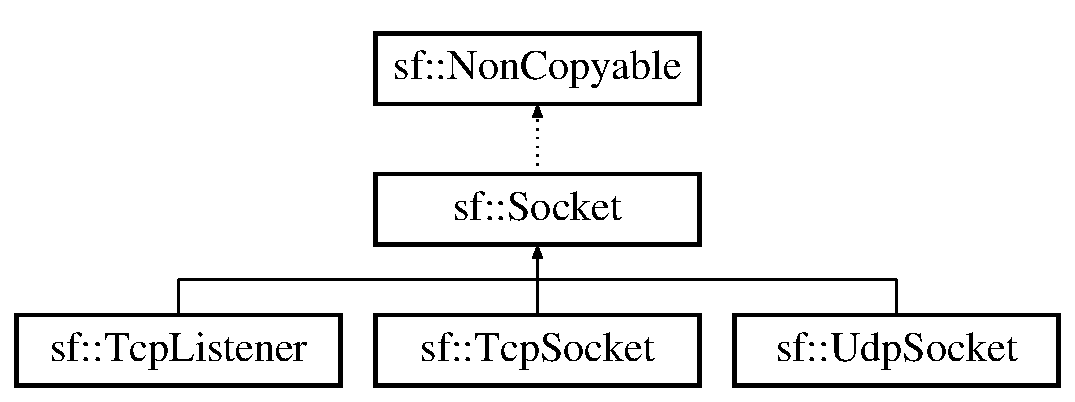
\includegraphics[height=3.000000cm]{classsf_1_1Socket}
\end{center}
\end{figure}
\subsection*{Public Types}
\begin{DoxyCompactItemize}
\item 
enum \hyperlink{classsf_1_1Socket_a51bf0fd51057b98a10fbb866246176dc}{Status} \{ \hyperlink{classsf_1_1Socket_a51bf0fd51057b98a10fbb866246176dca1de3a85bc56d3ae85b3d0f3cfd04ae90}{Done}, 
\hyperlink{classsf_1_1Socket_a51bf0fd51057b98a10fbb866246176dca8554848daae98f996e131bdeed076c09}{Not\-Ready}, 
\hyperlink{classsf_1_1Socket_a51bf0fd51057b98a10fbb866246176dcab215141f756acdc23c67fad149710eb1}{Disconnected}, 
\hyperlink{classsf_1_1Socket_a51bf0fd51057b98a10fbb866246176dca1dc9854433a28c22e192721179a2df5d}{Error}
 \}
\begin{DoxyCompactList}\small\item\em Status codes that may be returned by socket functions. \end{DoxyCompactList}\item 
enum \{ \hyperlink{classsf_1_1Socket_a5deb2c955fd347259c3a20d27b2481aaa5a3c30fd128895403afc11076f461b19}{Any\-Port} = 0
 \}
\begin{DoxyCompactList}\small\item\em Some special values used by sockets. \end{DoxyCompactList}\end{DoxyCompactItemize}
\subsection*{Public Member Functions}
\begin{DoxyCompactItemize}
\item 
\hypertarget{classsf_1_1Socket_a79a4b5918f0b34a2f8db449089694788}{virtual \hyperlink{classsf_1_1Socket_a79a4b5918f0b34a2f8db449089694788}{$\sim$\-Socket} ()}\label{classsf_1_1Socket_a79a4b5918f0b34a2f8db449089694788}

\begin{DoxyCompactList}\small\item\em Destructor. \end{DoxyCompactList}\item 
void \hyperlink{classsf_1_1Socket_a165fc1423e281ea2714c70303d3a9782}{set\-Blocking} (bool blocking)
\begin{DoxyCompactList}\small\item\em Set the blocking state of the socket. \end{DoxyCompactList}\item 
bool \hyperlink{classsf_1_1Socket_a0ec0d831b015e32eb5935fd2a9f8c67c}{is\-Blocking} () const 
\begin{DoxyCompactList}\small\item\em Tell whether the socket is in blocking or non-\/blocking mode. \end{DoxyCompactList}\end{DoxyCompactItemize}
\subsection*{Protected Types}
\begin{DoxyCompactItemize}
\item 
enum \hyperlink{classsf_1_1Socket_a5d3ff44e56e68f02816bb0fabc34adf8}{Type} \{ \hyperlink{classsf_1_1Socket_a5d3ff44e56e68f02816bb0fabc34adf8acc02e97e90234b957eaad4dff7f22214}{Tcp}, 
\hyperlink{classsf_1_1Socket_a5d3ff44e56e68f02816bb0fabc34adf8a6ebf3094830db4820191a327f3cc6ce2}{Udp}
 \}
\begin{DoxyCompactList}\small\item\em Types of protocols that the socket can use. \end{DoxyCompactList}\end{DoxyCompactItemize}
\subsection*{Protected Member Functions}
\begin{DoxyCompactItemize}
\item 
\hyperlink{classsf_1_1Socket_a80ffb47ec0bafc83af019055d3e6a303}{Socket} (\hyperlink{classsf_1_1Socket_a5d3ff44e56e68f02816bb0fabc34adf8}{Type} type)
\begin{DoxyCompactList}\small\item\em Default constructor. \end{DoxyCompactList}\item 
Socket\-Handle \hyperlink{classsf_1_1Socket_ac0c63b13e61da8294bf54e888e97f9a3}{get\-Handle} () const 
\begin{DoxyCompactList}\small\item\em Return the internal handle of the socket. \end{DoxyCompactList}\item 
void \hyperlink{classsf_1_1Socket_aafbe140f4b1921e0d19e88cf7a61dcbc}{create} ()
\begin{DoxyCompactList}\small\item\em Create the internal representation of the socket. \end{DoxyCompactList}\item 
void \hyperlink{classsf_1_1Socket_af1dd898f7aa3ead7ff7b2d1c20e97781}{create} (Socket\-Handle handle)
\begin{DoxyCompactList}\small\item\em Create the internal representation of the socket from a socket handle. \end{DoxyCompactList}\item 
void \hyperlink{classsf_1_1Socket_a71f2f5c2aa99e01cafe824fee4c573be}{close} ()
\begin{DoxyCompactList}\small\item\em Close the socket gracefully. \end{DoxyCompactList}\end{DoxyCompactItemize}
\subsection*{Friends}
\begin{DoxyCompactItemize}
\item 
\hypertarget{classsf_1_1Socket_a23fafd48278ea4f8f9c25f1f0f43693c}{class {\bfseries Socket\-Selector}}\label{classsf_1_1Socket_a23fafd48278ea4f8f9c25f1f0f43693c}

\end{DoxyCompactItemize}


\subsection{Detailed Description}
Base class for all the socket types. 

This class mainly defines internal stuff to be used by derived classes.

The only public features that it defines, and which is therefore common to all the socket classes, is the blocking state. All sockets can be set as blocking or non-\/blocking.

In blocking mode, socket functions will hang until the operation completes, which means that the entire program (well, in fact the current thread if you use multiple ones) will be stuck waiting for your socket operation to complete.

In non-\/blocking mode, all the socket functions will return immediately. If the socket is not ready to complete the requested operation, the function simply returns the proper status code (\hyperlink{classsf_1_1Socket_a51bf0fd51057b98a10fbb866246176dca8554848daae98f996e131bdeed076c09}{Socket\-::\-Not\-Ready}).

The default mode, which is blocking, is the one that is generally used, in combination with threads or selectors. The non-\/blocking mode is rather used in real-\/time applications that run an endless loop that can poll the socket often enough, and cannot afford blocking this loop.

\begin{DoxySeeAlso}{See Also}
\hyperlink{classsf_1_1TcpListener}{sf\-::\-Tcp\-Listener}, \hyperlink{classsf_1_1TcpSocket}{sf\-::\-Tcp\-Socket}, \hyperlink{classsf_1_1UdpSocket}{sf\-::\-Udp\-Socket} 
\end{DoxySeeAlso}


Definition at line 45 of file Socket.\-hpp.



\subsection{Member Enumeration Documentation}
\hypertarget{classsf_1_1Socket_a5deb2c955fd347259c3a20d27b2481aa}{\subsubsection[{anonymous enum}]{\setlength{\rightskip}{0pt plus 5cm}anonymous enum}}\label{classsf_1_1Socket_a5deb2c955fd347259c3a20d27b2481aa}


Some special values used by sockets. 

\begin{Desc}
\item[Enumerator]\par
\begin{description}
\index{Any\-Port@{Any\-Port}!sf\-::\-Socket@{sf\-::\-Socket}}\index{sf\-::\-Socket@{sf\-::\-Socket}!Any\-Port@{Any\-Port}}\item[{\em 
\hypertarget{classsf_1_1Socket_a5deb2c955fd347259c3a20d27b2481aaa5a3c30fd128895403afc11076f461b19}{Any\-Port}\label{classsf_1_1Socket_a5deb2c955fd347259c3a20d27b2481aaa5a3c30fd128895403afc11076f461b19}
}]Special value that tells the system to pick any available port. \end{description}
\end{Desc}


Definition at line 65 of file Socket.\-hpp.

\hypertarget{classsf_1_1Socket_a51bf0fd51057b98a10fbb866246176dc}{\index{sf\-::\-Socket@{sf\-::\-Socket}!Status@{Status}}
\index{Status@{Status}!sf::Socket@{sf\-::\-Socket}}
\subsubsection[{Status}]{\setlength{\rightskip}{0pt plus 5cm}enum {\bf sf\-::\-Socket\-::\-Status}}}\label{classsf_1_1Socket_a51bf0fd51057b98a10fbb866246176dc}


Status codes that may be returned by socket functions. 

\begin{Desc}
\item[Enumerator]\par
\begin{description}
\index{Done@{Done}!sf\-::\-Socket@{sf\-::\-Socket}}\index{sf\-::\-Socket@{sf\-::\-Socket}!Done@{Done}}\item[{\em 
\hypertarget{classsf_1_1Socket_a51bf0fd51057b98a10fbb866246176dca1de3a85bc56d3ae85b3d0f3cfd04ae90}{Done}\label{classsf_1_1Socket_a51bf0fd51057b98a10fbb866246176dca1de3a85bc56d3ae85b3d0f3cfd04ae90}
}]The socket has sent / received the data. \index{Not\-Ready@{Not\-Ready}!sf\-::\-Socket@{sf\-::\-Socket}}\index{sf\-::\-Socket@{sf\-::\-Socket}!Not\-Ready@{Not\-Ready}}\item[{\em 
\hypertarget{classsf_1_1Socket_a51bf0fd51057b98a10fbb866246176dca8554848daae98f996e131bdeed076c09}{Not\-Ready}\label{classsf_1_1Socket_a51bf0fd51057b98a10fbb866246176dca8554848daae98f996e131bdeed076c09}
}]The socket is not ready to send / receive data yet. \index{Disconnected@{Disconnected}!sf\-::\-Socket@{sf\-::\-Socket}}\index{sf\-::\-Socket@{sf\-::\-Socket}!Disconnected@{Disconnected}}\item[{\em 
\hypertarget{classsf_1_1Socket_a51bf0fd51057b98a10fbb866246176dcab215141f756acdc23c67fad149710eb1}{Disconnected}\label{classsf_1_1Socket_a51bf0fd51057b98a10fbb866246176dcab215141f756acdc23c67fad149710eb1}
}]The T\-C\-P socket has been disconnected. \index{Error@{Error}!sf\-::\-Socket@{sf\-::\-Socket}}\index{sf\-::\-Socket@{sf\-::\-Socket}!Error@{Error}}\item[{\em 
\hypertarget{classsf_1_1Socket_a51bf0fd51057b98a10fbb866246176dca1dc9854433a28c22e192721179a2df5d}{Error}\label{classsf_1_1Socket_a51bf0fd51057b98a10fbb866246176dca1dc9854433a28c22e192721179a2df5d}
}]An unexpected error happened. \end{description}
\end{Desc}


Definition at line 53 of file Socket.\-hpp.

\hypertarget{classsf_1_1Socket_a5d3ff44e56e68f02816bb0fabc34adf8}{\index{sf\-::\-Socket@{sf\-::\-Socket}!Type@{Type}}
\index{Type@{Type}!sf::Socket@{sf\-::\-Socket}}
\subsubsection[{Type}]{\setlength{\rightskip}{0pt plus 5cm}enum {\bf sf\-::\-Socket\-::\-Type}\hspace{0.3cm}{\ttfamily [protected]}}}\label{classsf_1_1Socket_a5d3ff44e56e68f02816bb0fabc34adf8}


Types of protocols that the socket can use. 

\begin{Desc}
\item[Enumerator]\par
\begin{description}
\index{Tcp@{Tcp}!sf\-::\-Socket@{sf\-::\-Socket}}\index{sf\-::\-Socket@{sf\-::\-Socket}!Tcp@{Tcp}}\item[{\em 
\hypertarget{classsf_1_1Socket_a5d3ff44e56e68f02816bb0fabc34adf8acc02e97e90234b957eaad4dff7f22214}{Tcp}\label{classsf_1_1Socket_a5d3ff44e56e68f02816bb0fabc34adf8acc02e97e90234b957eaad4dff7f22214}
}]T\-C\-P protocol. \index{Udp@{Udp}!sf\-::\-Socket@{sf\-::\-Socket}}\index{sf\-::\-Socket@{sf\-::\-Socket}!Udp@{Udp}}\item[{\em 
\hypertarget{classsf_1_1Socket_a5d3ff44e56e68f02816bb0fabc34adf8a6ebf3094830db4820191a327f3cc6ce2}{Udp}\label{classsf_1_1Socket_a5d3ff44e56e68f02816bb0fabc34adf8a6ebf3094830db4820191a327f3cc6ce2}
}]U\-D\-P protocol. \end{description}
\end{Desc}


Definition at line 113 of file Socket.\-hpp.



\subsection{Constructor \& Destructor Documentation}
\hypertarget{classsf_1_1Socket_a80ffb47ec0bafc83af019055d3e6a303}{\index{sf\-::\-Socket@{sf\-::\-Socket}!Socket@{Socket}}
\index{Socket@{Socket}!sf::Socket@{sf\-::\-Socket}}
\subsubsection[{Socket}]{\setlength{\rightskip}{0pt plus 5cm}sf\-::\-Socket\-::\-Socket (
\begin{DoxyParamCaption}
\item[{{\bf Type}}]{type}
\end{DoxyParamCaption}
)\hspace{0.3cm}{\ttfamily [protected]}}}\label{classsf_1_1Socket_a80ffb47ec0bafc83af019055d3e6a303}


Default constructor. 

This constructor can only be accessed by derived classes.


\begin{DoxyParams}{Parameters}
{\em type} & Type of the socket (T\-C\-P or U\-D\-P) \\
\hline
\end{DoxyParams}


\subsection{Member Function Documentation}
\hypertarget{classsf_1_1Socket_a71f2f5c2aa99e01cafe824fee4c573be}{\index{sf\-::\-Socket@{sf\-::\-Socket}!close@{close}}
\index{close@{close}!sf::Socket@{sf\-::\-Socket}}
\subsubsection[{close}]{\setlength{\rightskip}{0pt plus 5cm}void sf\-::\-Socket\-::close (
\begin{DoxyParamCaption}
{}
\end{DoxyParamCaption}
)\hspace{0.3cm}{\ttfamily [protected]}}}\label{classsf_1_1Socket_a71f2f5c2aa99e01cafe824fee4c573be}


Close the socket gracefully. 

This function can only be accessed by derived classes. \hypertarget{classsf_1_1Socket_aafbe140f4b1921e0d19e88cf7a61dcbc}{\index{sf\-::\-Socket@{sf\-::\-Socket}!create@{create}}
\index{create@{create}!sf::Socket@{sf\-::\-Socket}}
\subsubsection[{create}]{\setlength{\rightskip}{0pt plus 5cm}void sf\-::\-Socket\-::create (
\begin{DoxyParamCaption}
{}
\end{DoxyParamCaption}
)\hspace{0.3cm}{\ttfamily [protected]}}}\label{classsf_1_1Socket_aafbe140f4b1921e0d19e88cf7a61dcbc}


Create the internal representation of the socket. 

This function can only be accessed by derived classes. \hypertarget{classsf_1_1Socket_af1dd898f7aa3ead7ff7b2d1c20e97781}{\index{sf\-::\-Socket@{sf\-::\-Socket}!create@{create}}
\index{create@{create}!sf::Socket@{sf\-::\-Socket}}
\subsubsection[{create}]{\setlength{\rightskip}{0pt plus 5cm}void sf\-::\-Socket\-::create (
\begin{DoxyParamCaption}
\item[{Socket\-Handle}]{handle}
\end{DoxyParamCaption}
)\hspace{0.3cm}{\ttfamily [protected]}}}\label{classsf_1_1Socket_af1dd898f7aa3ead7ff7b2d1c20e97781}


Create the internal representation of the socket from a socket handle. 

This function can only be accessed by derived classes.


\begin{DoxyParams}{Parameters}
{\em handle} & O\-S-\/specific handle of the socket to wrap \\
\hline
\end{DoxyParams}
\hypertarget{classsf_1_1Socket_ac0c63b13e61da8294bf54e888e97f9a3}{\index{sf\-::\-Socket@{sf\-::\-Socket}!get\-Handle@{get\-Handle}}
\index{get\-Handle@{get\-Handle}!sf::Socket@{sf\-::\-Socket}}
\subsubsection[{get\-Handle}]{\setlength{\rightskip}{0pt plus 5cm}Socket\-Handle sf\-::\-Socket\-::get\-Handle (
\begin{DoxyParamCaption}
{}
\end{DoxyParamCaption}
) const\hspace{0.3cm}{\ttfamily [protected]}}}\label{classsf_1_1Socket_ac0c63b13e61da8294bf54e888e97f9a3}


Return the internal handle of the socket. 

The returned handle may be invalid if the socket was not created yet (or already destroyed). This function can only be accessed by derived classes.

\begin{DoxyReturn}{Returns}
The internal (O\-S-\/specific) handle of the socket 
\end{DoxyReturn}
\hypertarget{classsf_1_1Socket_a0ec0d831b015e32eb5935fd2a9f8c67c}{\index{sf\-::\-Socket@{sf\-::\-Socket}!is\-Blocking@{is\-Blocking}}
\index{is\-Blocking@{is\-Blocking}!sf::Socket@{sf\-::\-Socket}}
\subsubsection[{is\-Blocking}]{\setlength{\rightskip}{0pt plus 5cm}bool sf\-::\-Socket\-::is\-Blocking (
\begin{DoxyParamCaption}
{}
\end{DoxyParamCaption}
) const}}\label{classsf_1_1Socket_a0ec0d831b015e32eb5935fd2a9f8c67c}


Tell whether the socket is in blocking or non-\/blocking mode. 

\begin{DoxyReturn}{Returns}
True if the socket is blocking, false otherwise
\end{DoxyReturn}
\begin{DoxySeeAlso}{See Also}
\hyperlink{classsf_1_1Socket_a165fc1423e281ea2714c70303d3a9782}{set\-Blocking} 
\end{DoxySeeAlso}
\hypertarget{classsf_1_1Socket_a165fc1423e281ea2714c70303d3a9782}{\index{sf\-::\-Socket@{sf\-::\-Socket}!set\-Blocking@{set\-Blocking}}
\index{set\-Blocking@{set\-Blocking}!sf::Socket@{sf\-::\-Socket}}
\subsubsection[{set\-Blocking}]{\setlength{\rightskip}{0pt plus 5cm}void sf\-::\-Socket\-::set\-Blocking (
\begin{DoxyParamCaption}
\item[{bool}]{blocking}
\end{DoxyParamCaption}
)}}\label{classsf_1_1Socket_a165fc1423e281ea2714c70303d3a9782}


Set the blocking state of the socket. 

In blocking mode, calls will not return until they have completed their task. For example, a call to Receive in blocking mode won't return until some data was actually received. In non-\/blocking mode, calls will always return immediately, using the return code to signal whether there was data available or not. By default, all sockets are blocking.


\begin{DoxyParams}{Parameters}
{\em blocking} & True to set the socket as blocking, false for non-\/blocking\\
\hline
\end{DoxyParams}
\begin{DoxySeeAlso}{See Also}
\hyperlink{classsf_1_1Socket_a0ec0d831b015e32eb5935fd2a9f8c67c}{is\-Blocking} 
\end{DoxySeeAlso}


The documentation for this class was generated from the following file\-:\begin{DoxyCompactItemize}
\item 
/home/z\-Zelman/\-Dropbox/\-Placeholder-\/\-R\-T\-S/\-S\-F\-M\-L-\/2.\-1/include/\-S\-F\-M\-L/\-Network/Socket.\-hpp\end{DoxyCompactItemize}

\hypertarget{classsf_1_1SocketSelector}{\section{sf\-:\-:Socket\-Selector Class Reference}
\label{classsf_1_1SocketSelector}\index{sf\-::\-Socket\-Selector@{sf\-::\-Socket\-Selector}}
}


Multiplexer that allows to read from multiple sockets.  




{\ttfamily \#include $<$Socket\-Selector.\-hpp$>$}

\subsection*{Public Member Functions}
\begin{DoxyCompactItemize}
\item 
\hypertarget{classsf_1_1SocketSelector_a741959c5158aeb1e4457cad47d90f76b}{\hyperlink{classsf_1_1SocketSelector_a741959c5158aeb1e4457cad47d90f76b}{Socket\-Selector} ()}\label{classsf_1_1SocketSelector_a741959c5158aeb1e4457cad47d90f76b}

\begin{DoxyCompactList}\small\item\em Default constructor. \end{DoxyCompactList}\item 
\hyperlink{classsf_1_1SocketSelector_a50b1b955eb7ecb2e7c2764f3f4722fbf}{Socket\-Selector} (const \hyperlink{classsf_1_1SocketSelector}{Socket\-Selector} \&copy)
\begin{DoxyCompactList}\small\item\em Copy constructor. \end{DoxyCompactList}\item 
\hypertarget{classsf_1_1SocketSelector_a9069cd61208260b8ed9cf233afa1f73d}{\hyperlink{classsf_1_1SocketSelector_a9069cd61208260b8ed9cf233afa1f73d}{$\sim$\-Socket\-Selector} ()}\label{classsf_1_1SocketSelector_a9069cd61208260b8ed9cf233afa1f73d}

\begin{DoxyCompactList}\small\item\em Destructor. \end{DoxyCompactList}\item 
void \hyperlink{classsf_1_1SocketSelector_ade952013232802ff7b9b33668f8d2096}{add} (\hyperlink{classsf_1_1Socket}{Socket} \&socket)
\begin{DoxyCompactList}\small\item\em Add a new socket to the selector. \end{DoxyCompactList}\item 
void \hyperlink{classsf_1_1SocketSelector_a98b6ab693a65b82caa375639232357c1}{remove} (\hyperlink{classsf_1_1Socket}{Socket} \&socket)
\begin{DoxyCompactList}\small\item\em Remove a socket from the selector. \end{DoxyCompactList}\item 
void \hyperlink{classsf_1_1SocketSelector_a76e650acb0199d4be91e90a493fbc91a}{clear} ()
\begin{DoxyCompactList}\small\item\em Remove all the sockets stored in the selector. \end{DoxyCompactList}\item 
bool \hyperlink{classsf_1_1SocketSelector_a9cfda5475f17925e65889394d70af702}{wait} (\hyperlink{classsf_1_1Time}{Time} timeout=\hyperlink{classsf_1_1Time_a8db127b632fa8da21550e7282af11fa0}{Time\-::\-Zero})
\begin{DoxyCompactList}\small\item\em Wait until one or more sockets are ready to receive. \end{DoxyCompactList}\item 
bool \hyperlink{classsf_1_1SocketSelector_a8e67b463db05eadb4d356992c896833c}{is\-Ready} (\hyperlink{classsf_1_1Socket}{Socket} \&socket) const 
\begin{DoxyCompactList}\small\item\em \hyperlink{classTest}{Test} a socket to know if it is ready to receive data. \end{DoxyCompactList}\item 
\hyperlink{classsf_1_1SocketSelector}{Socket\-Selector} \& \hyperlink{classsf_1_1SocketSelector_ae6395c7a8d29a9ea14939cc5d1ba3a33}{operator=} (const \hyperlink{classsf_1_1SocketSelector}{Socket\-Selector} \&right)
\begin{DoxyCompactList}\small\item\em Overload of assignment operator. \end{DoxyCompactList}\end{DoxyCompactItemize}


\subsection{Detailed Description}
Multiplexer that allows to read from multiple sockets. 

\hyperlink{classsf_1_1Socket}{Socket} selectors provide a way to wait until some data is available on a set of sockets, instead of just one. This is convenient when you have multiple sockets that may possibly receive data, but you don't know which one will be ready first. In particular, it avoids to use a thread for each socket; with selectors, a single thread can handle all the sockets.

All types of sockets can be used in a selector\-: \begin{DoxyItemize}
\item \hyperlink{classsf_1_1TcpListener}{sf\-::\-Tcp\-Listener} \item \hyperlink{classsf_1_1TcpSocket}{sf\-::\-Tcp\-Socket} \item \hyperlink{classsf_1_1UdpSocket}{sf\-::\-Udp\-Socket}\end{DoxyItemize}
A selector doesn't store its own copies of the sockets (socket classes are not copyable anyway), it simply keeps a reference to the original sockets that you pass to the \char`\"{}add\char`\"{} function. Therefore, you can't use the selector as a socket container, you must store them oustide and make sure that they are alive as long as they are used in the selector.

Using a selector is simple\-: \begin{DoxyItemize}
\item populate the selector with all the sockets that you want to observe \item make it wait until there is data available on any of the sockets \item test each socket to find out which ones are ready\end{DoxyItemize}
Usage example\-: 
\begin{DoxyCode}
\textcolor{comment}{// Create a socket to listen to new connections}
\hyperlink{classsf_1_1TcpListener}{sf::TcpListener} listener;
listener.\hyperlink{classsf_1_1TcpListener_a409d9350d3abfea9636df8cf4a61004e}{listen}(55001);

\textcolor{comment}{// Create a list to store the future clients}
std::list<sf::TcpSocket*> clients;

\textcolor{comment}{// Create a selector}
\hyperlink{classsf_1_1SocketSelector}{sf::SocketSelector} selector;

\textcolor{comment}{// Add the listener to the selector}
selector.\hyperlink{classsf_1_1SocketSelector_ade952013232802ff7b9b33668f8d2096}{add}(listener);

\textcolor{comment}{// Endless loop that waits for new connections}
\textcolor{keywordflow}{while} (running)
\{
    \textcolor{comment}{// Make the selector wait for data on any socket}
    \textcolor{keywordflow}{if} (selector.\hyperlink{classsf_1_1SocketSelector_a9cfda5475f17925e65889394d70af702}{wait}())
    \{
        \textcolor{comment}{// Test the listener}
        \textcolor{keywordflow}{if} (selector.\hyperlink{classsf_1_1SocketSelector_a8e67b463db05eadb4d356992c896833c}{isReady}(listener))
        \{
            \textcolor{comment}{// The listener is ready: there is a pending connection}
            \hyperlink{classsf_1_1TcpSocket}{sf::TcpSocket}* client = \textcolor{keyword}{new} \hyperlink{classsf_1_1TcpSocket}{sf::TcpSocket};
            \textcolor{keywordflow}{if} (listener.\hyperlink{classsf_1_1TcpListener_ae2c83ce5a64d50b68180c46bef0a7346}{accept}(*client) == \hyperlink{classsf_1_1Socket_a51bf0fd51057b98a10fbb866246176dca1de3a85bc56d3ae85b3d0f3cfd04ae90}{sf::Socket::Done})
            \{
                \textcolor{comment}{// Add the new client to the clients list}
                clients.push\_back(client);

                \textcolor{comment}{// Add the new client to the selector so that we will}
                \textcolor{comment}{// be notified when he sends something}
                selector.\hyperlink{classsf_1_1SocketSelector_ade952013232802ff7b9b33668f8d2096}{add}(*client);
            \}
            \textcolor{keywordflow}{else}
            \{
                \textcolor{comment}{// Error, we won't get a new connection, delete the socket}
                \textcolor{keyword}{delete} client;
            \}
        \}
        \textcolor{keywordflow}{else}
        \{
            \textcolor{comment}{// The listener socket is not ready, test all other sockets (the clients)}
            \textcolor{keywordflow}{for} (std::list<sf::TcpSocket*>::iterator it = clients.begin(); it != clients.end(); ++it)
            \{
                \hyperlink{classsf_1_1TcpSocket}{sf::TcpSocket}& client = **it;
                \textcolor{keywordflow}{if} (selector.\hyperlink{classsf_1_1SocketSelector_a8e67b463db05eadb4d356992c896833c}{isReady}(client))
                \{
                    \textcolor{comment}{// The client has sent some data, we can receive it}
                    \hyperlink{classsf_1_1Packet}{sf::Packet} packet;
                    \textcolor{keywordflow}{if} (client.\hyperlink{classsf_1_1TcpSocket_a90ce50811ea61d4f00efc62bb99ae1af}{receive}(packet) == \hyperlink{classsf_1_1Socket_a51bf0fd51057b98a10fbb866246176dca1de3a85bc56d3ae85b3d0f3cfd04ae90}{sf::Socket::Done})
                    \{
                        ...
                    \}
                \}
            \}
        \}
    \}
\}
\end{DoxyCode}


\begin{DoxySeeAlso}{See Also}
\hyperlink{classsf_1_1Socket}{sf\-::\-Socket} 
\end{DoxySeeAlso}


Definition at line 43 of file Socket\-Selector.\-hpp.



\subsection{Constructor \& Destructor Documentation}
\hypertarget{classsf_1_1SocketSelector_a50b1b955eb7ecb2e7c2764f3f4722fbf}{\index{sf\-::\-Socket\-Selector@{sf\-::\-Socket\-Selector}!Socket\-Selector@{Socket\-Selector}}
\index{Socket\-Selector@{Socket\-Selector}!sf::SocketSelector@{sf\-::\-Socket\-Selector}}
\subsubsection[{Socket\-Selector}]{\setlength{\rightskip}{0pt plus 5cm}sf\-::\-Socket\-Selector\-::\-Socket\-Selector (
\begin{DoxyParamCaption}
\item[{const {\bf Socket\-Selector} \&}]{copy}
\end{DoxyParamCaption}
)}}\label{classsf_1_1SocketSelector_a50b1b955eb7ecb2e7c2764f3f4722fbf}


Copy constructor. 


\begin{DoxyParams}{Parameters}
{\em copy} & Instance to copy \\
\hline
\end{DoxyParams}


\subsection{Member Function Documentation}
\hypertarget{classsf_1_1SocketSelector_ade952013232802ff7b9b33668f8d2096}{\index{sf\-::\-Socket\-Selector@{sf\-::\-Socket\-Selector}!add@{add}}
\index{add@{add}!sf::SocketSelector@{sf\-::\-Socket\-Selector}}
\subsubsection[{add}]{\setlength{\rightskip}{0pt plus 5cm}void sf\-::\-Socket\-Selector\-::add (
\begin{DoxyParamCaption}
\item[{{\bf Socket} \&}]{socket}
\end{DoxyParamCaption}
)}}\label{classsf_1_1SocketSelector_ade952013232802ff7b9b33668f8d2096}


Add a new socket to the selector. 

This function keeps a weak reference to the socket, so you have to make sure that the socket is not destroyed while it is stored in the selector. This function does nothing if the socket is not valid.


\begin{DoxyParams}{Parameters}
{\em socket} & Reference to the socket to add\\
\hline
\end{DoxyParams}
\begin{DoxySeeAlso}{See Also}
\hyperlink{classsf_1_1SocketSelector_a98b6ab693a65b82caa375639232357c1}{remove}, \hyperlink{classsf_1_1SocketSelector_a76e650acb0199d4be91e90a493fbc91a}{clear} 
\end{DoxySeeAlso}
\hypertarget{classsf_1_1SocketSelector_a76e650acb0199d4be91e90a493fbc91a}{\index{sf\-::\-Socket\-Selector@{sf\-::\-Socket\-Selector}!clear@{clear}}
\index{clear@{clear}!sf::SocketSelector@{sf\-::\-Socket\-Selector}}
\subsubsection[{clear}]{\setlength{\rightskip}{0pt plus 5cm}void sf\-::\-Socket\-Selector\-::clear (
\begin{DoxyParamCaption}
{}
\end{DoxyParamCaption}
)}}\label{classsf_1_1SocketSelector_a76e650acb0199d4be91e90a493fbc91a}


Remove all the sockets stored in the selector. 

This function doesn't destroy any instance, it simply removes all the references that the selector has to external sockets.

\begin{DoxySeeAlso}{See Also}
\hyperlink{classsf_1_1SocketSelector_ade952013232802ff7b9b33668f8d2096}{add}, \hyperlink{classsf_1_1SocketSelector_a98b6ab693a65b82caa375639232357c1}{remove} 
\end{DoxySeeAlso}
\hypertarget{classsf_1_1SocketSelector_a8e67b463db05eadb4d356992c896833c}{\index{sf\-::\-Socket\-Selector@{sf\-::\-Socket\-Selector}!is\-Ready@{is\-Ready}}
\index{is\-Ready@{is\-Ready}!sf::SocketSelector@{sf\-::\-Socket\-Selector}}
\subsubsection[{is\-Ready}]{\setlength{\rightskip}{0pt plus 5cm}bool sf\-::\-Socket\-Selector\-::is\-Ready (
\begin{DoxyParamCaption}
\item[{{\bf Socket} \&}]{socket}
\end{DoxyParamCaption}
) const}}\label{classsf_1_1SocketSelector_a8e67b463db05eadb4d356992c896833c}


\hyperlink{classTest}{Test} a socket to know if it is ready to receive data. 

This function must be used after a call to Wait, to know which sockets are ready to receive data. If a socket is ready, a call to receive will never block because we know that there is data available to read. Note that if this function returns true for a \hyperlink{classsf_1_1TcpListener}{Tcp\-Listener}, this means that it is ready to accept a new connection.


\begin{DoxyParams}{Parameters}
{\em socket} & \hyperlink{classsf_1_1Socket}{Socket} to test\\
\hline
\end{DoxyParams}
\begin{DoxyReturn}{Returns}
True if the socket is ready to read, false otherwise
\end{DoxyReturn}
\begin{DoxySeeAlso}{See Also}
\hyperlink{classsf_1_1SocketSelector_a8e67b463db05eadb4d356992c896833c}{is\-Ready} 
\end{DoxySeeAlso}
\hypertarget{classsf_1_1SocketSelector_ae6395c7a8d29a9ea14939cc5d1ba3a33}{\index{sf\-::\-Socket\-Selector@{sf\-::\-Socket\-Selector}!operator=@{operator=}}
\index{operator=@{operator=}!sf::SocketSelector@{sf\-::\-Socket\-Selector}}
\subsubsection[{operator=}]{\setlength{\rightskip}{0pt plus 5cm}{\bf Socket\-Selector}\& sf\-::\-Socket\-Selector\-::operator= (
\begin{DoxyParamCaption}
\item[{const {\bf Socket\-Selector} \&}]{right}
\end{DoxyParamCaption}
)}}\label{classsf_1_1SocketSelector_ae6395c7a8d29a9ea14939cc5d1ba3a33}


Overload of assignment operator. 


\begin{DoxyParams}{Parameters}
{\em right} & Instance to assign\\
\hline
\end{DoxyParams}
\begin{DoxyReturn}{Returns}
Reference to self 
\end{DoxyReturn}
\hypertarget{classsf_1_1SocketSelector_a98b6ab693a65b82caa375639232357c1}{\index{sf\-::\-Socket\-Selector@{sf\-::\-Socket\-Selector}!remove@{remove}}
\index{remove@{remove}!sf::SocketSelector@{sf\-::\-Socket\-Selector}}
\subsubsection[{remove}]{\setlength{\rightskip}{0pt plus 5cm}void sf\-::\-Socket\-Selector\-::remove (
\begin{DoxyParamCaption}
\item[{{\bf Socket} \&}]{socket}
\end{DoxyParamCaption}
)}}\label{classsf_1_1SocketSelector_a98b6ab693a65b82caa375639232357c1}


Remove a socket from the selector. 

This function doesn't destroy the socket, it simply removes the reference that the selector has to it.


\begin{DoxyParams}{Parameters}
{\em socket} & Reference to the socket to remove\\
\hline
\end{DoxyParams}
\begin{DoxySeeAlso}{See Also}
\hyperlink{classsf_1_1SocketSelector_ade952013232802ff7b9b33668f8d2096}{add}, \hyperlink{classsf_1_1SocketSelector_a76e650acb0199d4be91e90a493fbc91a}{clear} 
\end{DoxySeeAlso}
\hypertarget{classsf_1_1SocketSelector_a9cfda5475f17925e65889394d70af702}{\index{sf\-::\-Socket\-Selector@{sf\-::\-Socket\-Selector}!wait@{wait}}
\index{wait@{wait}!sf::SocketSelector@{sf\-::\-Socket\-Selector}}
\subsubsection[{wait}]{\setlength{\rightskip}{0pt plus 5cm}bool sf\-::\-Socket\-Selector\-::wait (
\begin{DoxyParamCaption}
\item[{{\bf Time}}]{timeout = {\ttfamily {\bf Time\-::\-Zero}}}
\end{DoxyParamCaption}
)}}\label{classsf_1_1SocketSelector_a9cfda5475f17925e65889394d70af702}


Wait until one or more sockets are ready to receive. 

This function returns as soon as at least one socket has some data available to be received. To know which sockets are ready, use the is\-Ready function. If you use a timeout and no socket is ready before the timeout is over, the function returns false.


\begin{DoxyParams}{Parameters}
{\em timeout} & Maximum time to wait, (use \hyperlink{classsf_1_1Time_a8db127b632fa8da21550e7282af11fa0}{Time\-::\-Zero} for infinity)\\
\hline
\end{DoxyParams}
\begin{DoxyReturn}{Returns}
True if there are sockets ready, false otherwise
\end{DoxyReturn}
\begin{DoxySeeAlso}{See Also}
\hyperlink{classsf_1_1SocketSelector_a8e67b463db05eadb4d356992c896833c}{is\-Ready} 
\end{DoxySeeAlso}


The documentation for this class was generated from the following file\-:\begin{DoxyCompactItemize}
\item 
/home/z\-Zelman/\-Dropbox/\-Placeholder-\/\-R\-T\-S/\-S\-F\-M\-L-\/2.\-1/include/\-S\-F\-M\-L/\-Network/Socket\-Selector.\-hpp\end{DoxyCompactItemize}

\hypertarget{classsf_1_1Sound}{\section{sf\-:\-:Sound Class Reference}
\label{classsf_1_1Sound}\index{sf\-::\-Sound@{sf\-::\-Sound}}
}


Regular sound that can be played in the audio environment.  




{\ttfamily \#include $<$Sound.\-hpp$>$}

Inheritance diagram for sf\-:\-:Sound\-:\begin{figure}[H]
\begin{center}
\leavevmode
\includegraphics[height=2.000000cm]{classsf_1_1Sound}
\end{center}
\end{figure}
\subsection*{Public Member Functions}
\begin{DoxyCompactItemize}
\item 
\hypertarget{classsf_1_1Sound_a36ab74beaaa953d9879c933ddd246282}{\hyperlink{classsf_1_1Sound_a36ab74beaaa953d9879c933ddd246282}{Sound} ()}\label{classsf_1_1Sound_a36ab74beaaa953d9879c933ddd246282}

\begin{DoxyCompactList}\small\item\em Default constructor. \end{DoxyCompactList}\item 
\hyperlink{classsf_1_1Sound_a3b1cfc19a856d4ff8c079ee41bb78e69}{Sound} (const \hyperlink{classsf_1_1SoundBuffer}{Sound\-Buffer} \&buffer)
\begin{DoxyCompactList}\small\item\em Construct the sound with a buffer. \end{DoxyCompactList}\item 
\hyperlink{classsf_1_1Sound_ae05eeed6377932694d86b3011be366c0}{Sound} (const \hyperlink{classsf_1_1Sound}{Sound} \&copy)
\begin{DoxyCompactList}\small\item\em Copy constructor. \end{DoxyCompactList}\item 
\hypertarget{classsf_1_1Sound_ad0792c35310eba2dffd8489c80fad076}{\hyperlink{classsf_1_1Sound_ad0792c35310eba2dffd8489c80fad076}{$\sim$\-Sound} ()}\label{classsf_1_1Sound_ad0792c35310eba2dffd8489c80fad076}

\begin{DoxyCompactList}\small\item\em Destructor. \end{DoxyCompactList}\item 
void \hyperlink{classsf_1_1Sound_a2953ffe632536e72e696fd880ced2532}{play} ()
\begin{DoxyCompactList}\small\item\em Start or resume playing the sound. \end{DoxyCompactList}\item 
void \hyperlink{classsf_1_1Sound_a5eeb25815bfa8cdc4a6cc000b7b19ad5}{pause} ()
\begin{DoxyCompactList}\small\item\em Pause the sound. \end{DoxyCompactList}\item 
void \hyperlink{classsf_1_1Sound_aa9c91c34f7c6d344d5ee9b997511f754}{stop} ()
\begin{DoxyCompactList}\small\item\em stop playing the sound \end{DoxyCompactList}\item 
void \hyperlink{classsf_1_1Sound_a8b395e9713d0efa48a18628c8ec1972e}{set\-Buffer} (const \hyperlink{classsf_1_1SoundBuffer}{Sound\-Buffer} \&buffer)
\begin{DoxyCompactList}\small\item\em Set the source buffer containing the audio data to play. \end{DoxyCompactList}\item 
void \hyperlink{classsf_1_1Sound_af23ab4f78f975bbabac031102321612b}{set\-Loop} (bool loop)
\begin{DoxyCompactList}\small\item\em Set whether or not the sound should loop after reaching the end. \end{DoxyCompactList}\item 
void \hyperlink{classsf_1_1Sound_ab905677846558042022dd6ab15cddff0}{set\-Playing\-Offset} (\hyperlink{classsf_1_1Time}{Time} time\-Offset)
\begin{DoxyCompactList}\small\item\em Change the current playing position of the sound. \end{DoxyCompactList}\item 
const \hyperlink{classsf_1_1SoundBuffer}{Sound\-Buffer} $\ast$ \hyperlink{classsf_1_1Sound_a5f2f1ec6603f73625f393f0e9ab64476}{get\-Buffer} () const 
\begin{DoxyCompactList}\small\item\em Get the audio buffer attached to the sound. \end{DoxyCompactList}\item 
bool \hyperlink{classsf_1_1Sound_a603fbd32b519ae1680c40d8ddfc7ea51}{get\-Loop} () const 
\begin{DoxyCompactList}\small\item\em Tell whether or not the sound is in loop mode. \end{DoxyCompactList}\item 
\hyperlink{classsf_1_1Time}{Time} \hyperlink{classsf_1_1Sound_aeca741a3442d9934369a986ad40f19c0}{get\-Playing\-Offset} () const 
\begin{DoxyCompactList}\small\item\em Get the current playing position of the sound. \end{DoxyCompactList}\item 
\hyperlink{classsf_1_1SoundSource_ac43af72c98c077500b239bc75b812f03}{Status} \hyperlink{classsf_1_1Sound_ae8b4084ff8f460b7a2bf9d39e846dab9}{get\-Status} () const 
\begin{DoxyCompactList}\small\item\em Get the current status of the sound (stopped, paused, playing) \end{DoxyCompactList}\item 
\hyperlink{classsf_1_1Sound}{Sound} \& \hyperlink{classsf_1_1Sound_a08c64c9c1dabeebc59fbf2540d81d4dd}{operator=} (const \hyperlink{classsf_1_1Sound}{Sound} \&right)
\begin{DoxyCompactList}\small\item\em Overload of assignment operator. \end{DoxyCompactList}\item 
void \hyperlink{classsf_1_1Sound_acb7289d45e06fb76b8292ac84beb82a7}{reset\-Buffer} ()
\begin{DoxyCompactList}\small\item\em Reset the internal buffer of the sound. \end{DoxyCompactList}\end{DoxyCompactItemize}
\subsection*{Additional Inherited Members}


\subsection{Detailed Description}
Regular sound that can be played in the audio environment. 

\hyperlink{classsf_1_1Sound}{sf\-::\-Sound} is the class to use to play sounds. It provides\-: \begin{DoxyItemize}
\item Control (play, pause, stop) \item Ability to modify output parameters in real-\/time (pitch, volume, ...) \item 3\-D spatial features (position, attenuation, ...).\end{DoxyItemize}
\hyperlink{classsf_1_1Sound}{sf\-::\-Sound} is perfect for playing short sounds that can fit in memory and require no latency, like foot steps or gun shots. For longer sounds, like background musics or long speeches, rather see \hyperlink{classsf_1_1Music}{sf\-::\-Music} (which is based on streaming).

In order to work, a sound must be given a buffer of audio data to play. Audio data (samples) is stored in \hyperlink{classsf_1_1SoundBuffer}{sf\-::\-Sound\-Buffer}, and attached to a sound with the \hyperlink{classsf_1_1Sound_a8b395e9713d0efa48a18628c8ec1972e}{set\-Buffer()} function. The buffer object attached to a sound must remain alive as long as the sound uses it. Note that multiple sounds can use the same sound buffer at the same time.

Usage example\-: 
\begin{DoxyCode}
\hyperlink{classsf_1_1SoundBuffer}{sf::SoundBuffer} buffer;
buffer.\hyperlink{classsf_1_1SoundBuffer_a2be6a8025c97eb622a7dff6cf2594394}{loadFromFile}(\textcolor{stringliteral}{"sound.wav"});

\hyperlink{classsf_1_1Sound}{sf::Sound} sound;
sound.\hyperlink{classsf_1_1Sound_a8b395e9713d0efa48a18628c8ec1972e}{setBuffer}(buffer);
sound.\hyperlink{classsf_1_1Sound_a2953ffe632536e72e696fd880ced2532}{play}();
\end{DoxyCode}


\begin{DoxySeeAlso}{See Also}
\hyperlink{classsf_1_1SoundBuffer}{sf\-::\-Sound\-Buffer}, \hyperlink{classsf_1_1Music}{sf\-::\-Music} 
\end{DoxySeeAlso}


Definition at line 45 of file Sound.\-hpp.



\subsection{Constructor \& Destructor Documentation}
\hypertarget{classsf_1_1Sound_a3b1cfc19a856d4ff8c079ee41bb78e69}{\index{sf\-::\-Sound@{sf\-::\-Sound}!Sound@{Sound}}
\index{Sound@{Sound}!sf::Sound@{sf\-::\-Sound}}
\subsubsection[{Sound}]{\setlength{\rightskip}{0pt plus 5cm}sf\-::\-Sound\-::\-Sound (
\begin{DoxyParamCaption}
\item[{const {\bf Sound\-Buffer} \&}]{buffer}
\end{DoxyParamCaption}
)\hspace{0.3cm}{\ttfamily [explicit]}}}\label{classsf_1_1Sound_a3b1cfc19a856d4ff8c079ee41bb78e69}


Construct the sound with a buffer. 


\begin{DoxyParams}{Parameters}
{\em buffer} & \hyperlink{classsf_1_1Sound}{Sound} buffer containing the audio data to play with the sound \\
\hline
\end{DoxyParams}
\hypertarget{classsf_1_1Sound_ae05eeed6377932694d86b3011be366c0}{\index{sf\-::\-Sound@{sf\-::\-Sound}!Sound@{Sound}}
\index{Sound@{Sound}!sf::Sound@{sf\-::\-Sound}}
\subsubsection[{Sound}]{\setlength{\rightskip}{0pt plus 5cm}sf\-::\-Sound\-::\-Sound (
\begin{DoxyParamCaption}
\item[{const {\bf Sound} \&}]{copy}
\end{DoxyParamCaption}
)}}\label{classsf_1_1Sound_ae05eeed6377932694d86b3011be366c0}


Copy constructor. 


\begin{DoxyParams}{Parameters}
{\em copy} & Instance to copy \\
\hline
\end{DoxyParams}


\subsection{Member Function Documentation}
\hypertarget{classsf_1_1Sound_a5f2f1ec6603f73625f393f0e9ab64476}{\index{sf\-::\-Sound@{sf\-::\-Sound}!get\-Buffer@{get\-Buffer}}
\index{get\-Buffer@{get\-Buffer}!sf::Sound@{sf\-::\-Sound}}
\subsubsection[{get\-Buffer}]{\setlength{\rightskip}{0pt plus 5cm}const {\bf Sound\-Buffer}$\ast$ sf\-::\-Sound\-::get\-Buffer (
\begin{DoxyParamCaption}
{}
\end{DoxyParamCaption}
) const}}\label{classsf_1_1Sound_a5f2f1ec6603f73625f393f0e9ab64476}


Get the audio buffer attached to the sound. 

\begin{DoxyReturn}{Returns}
\hyperlink{classsf_1_1Sound}{Sound} buffer attached to the sound (can be N\-U\-L\-L) 
\end{DoxyReturn}
\hypertarget{classsf_1_1Sound_a603fbd32b519ae1680c40d8ddfc7ea51}{\index{sf\-::\-Sound@{sf\-::\-Sound}!get\-Loop@{get\-Loop}}
\index{get\-Loop@{get\-Loop}!sf::Sound@{sf\-::\-Sound}}
\subsubsection[{get\-Loop}]{\setlength{\rightskip}{0pt plus 5cm}bool sf\-::\-Sound\-::get\-Loop (
\begin{DoxyParamCaption}
{}
\end{DoxyParamCaption}
) const}}\label{classsf_1_1Sound_a603fbd32b519ae1680c40d8ddfc7ea51}


Tell whether or not the sound is in loop mode. 

\begin{DoxyReturn}{Returns}
True if the sound is looping, false otherwise
\end{DoxyReturn}
\begin{DoxySeeAlso}{See Also}
\hyperlink{classsf_1_1Sound_af23ab4f78f975bbabac031102321612b}{set\-Loop} 
\end{DoxySeeAlso}
\hypertarget{classsf_1_1Sound_aeca741a3442d9934369a986ad40f19c0}{\index{sf\-::\-Sound@{sf\-::\-Sound}!get\-Playing\-Offset@{get\-Playing\-Offset}}
\index{get\-Playing\-Offset@{get\-Playing\-Offset}!sf::Sound@{sf\-::\-Sound}}
\subsubsection[{get\-Playing\-Offset}]{\setlength{\rightskip}{0pt plus 5cm}{\bf Time} sf\-::\-Sound\-::get\-Playing\-Offset (
\begin{DoxyParamCaption}
{}
\end{DoxyParamCaption}
) const}}\label{classsf_1_1Sound_aeca741a3442d9934369a986ad40f19c0}


Get the current playing position of the sound. 

\begin{DoxyReturn}{Returns}
Current playing position, from the beginning of the sound
\end{DoxyReturn}
\begin{DoxySeeAlso}{See Also}
\hyperlink{classsf_1_1Sound_ab905677846558042022dd6ab15cddff0}{set\-Playing\-Offset} 
\end{DoxySeeAlso}
\hypertarget{classsf_1_1Sound_ae8b4084ff8f460b7a2bf9d39e846dab9}{\index{sf\-::\-Sound@{sf\-::\-Sound}!get\-Status@{get\-Status}}
\index{get\-Status@{get\-Status}!sf::Sound@{sf\-::\-Sound}}
\subsubsection[{get\-Status}]{\setlength{\rightskip}{0pt plus 5cm}{\bf Status} sf\-::\-Sound\-::get\-Status (
\begin{DoxyParamCaption}
{}
\end{DoxyParamCaption}
) const}}\label{classsf_1_1Sound_ae8b4084ff8f460b7a2bf9d39e846dab9}


Get the current status of the sound (stopped, paused, playing) 

\begin{DoxyReturn}{Returns}
Current status of the sound 
\end{DoxyReturn}
\hypertarget{classsf_1_1Sound_a08c64c9c1dabeebc59fbf2540d81d4dd}{\index{sf\-::\-Sound@{sf\-::\-Sound}!operator=@{operator=}}
\index{operator=@{operator=}!sf::Sound@{sf\-::\-Sound}}
\subsubsection[{operator=}]{\setlength{\rightskip}{0pt plus 5cm}{\bf Sound}\& sf\-::\-Sound\-::operator= (
\begin{DoxyParamCaption}
\item[{const {\bf Sound} \&}]{right}
\end{DoxyParamCaption}
)}}\label{classsf_1_1Sound_a08c64c9c1dabeebc59fbf2540d81d4dd}


Overload of assignment operator. 


\begin{DoxyParams}{Parameters}
{\em right} & Instance to assign\\
\hline
\end{DoxyParams}
\begin{DoxyReturn}{Returns}
Reference to self 
\end{DoxyReturn}
\hypertarget{classsf_1_1Sound_a5eeb25815bfa8cdc4a6cc000b7b19ad5}{\index{sf\-::\-Sound@{sf\-::\-Sound}!pause@{pause}}
\index{pause@{pause}!sf::Sound@{sf\-::\-Sound}}
\subsubsection[{pause}]{\setlength{\rightskip}{0pt plus 5cm}void sf\-::\-Sound\-::pause (
\begin{DoxyParamCaption}
{}
\end{DoxyParamCaption}
)}}\label{classsf_1_1Sound_a5eeb25815bfa8cdc4a6cc000b7b19ad5}


Pause the sound. 

This function pauses the sound if it was playing, otherwise (sound already paused or stopped) it has no effect.

\begin{DoxySeeAlso}{See Also}
\hyperlink{classsf_1_1Sound_a2953ffe632536e72e696fd880ced2532}{play}, \hyperlink{classsf_1_1Sound_aa9c91c34f7c6d344d5ee9b997511f754}{stop} 
\end{DoxySeeAlso}
\hypertarget{classsf_1_1Sound_a2953ffe632536e72e696fd880ced2532}{\index{sf\-::\-Sound@{sf\-::\-Sound}!play@{play}}
\index{play@{play}!sf::Sound@{sf\-::\-Sound}}
\subsubsection[{play}]{\setlength{\rightskip}{0pt plus 5cm}void sf\-::\-Sound\-::play (
\begin{DoxyParamCaption}
{}
\end{DoxyParamCaption}
)}}\label{classsf_1_1Sound_a2953ffe632536e72e696fd880ced2532}


Start or resume playing the sound. 

This function starts the stream if it was stopped, resumes it if it was paused, and restarts it from beginning if it was it already playing. This function uses its own thread so that it doesn't block the rest of the program while the sound is played.

\begin{DoxySeeAlso}{See Also}
\hyperlink{classsf_1_1Sound_a5eeb25815bfa8cdc4a6cc000b7b19ad5}{pause}, \hyperlink{classsf_1_1Sound_aa9c91c34f7c6d344d5ee9b997511f754}{stop} 
\end{DoxySeeAlso}
\hypertarget{classsf_1_1Sound_acb7289d45e06fb76b8292ac84beb82a7}{\index{sf\-::\-Sound@{sf\-::\-Sound}!reset\-Buffer@{reset\-Buffer}}
\index{reset\-Buffer@{reset\-Buffer}!sf::Sound@{sf\-::\-Sound}}
\subsubsection[{reset\-Buffer}]{\setlength{\rightskip}{0pt plus 5cm}void sf\-::\-Sound\-::reset\-Buffer (
\begin{DoxyParamCaption}
{}
\end{DoxyParamCaption}
)}}\label{classsf_1_1Sound_acb7289d45e06fb76b8292ac84beb82a7}


Reset the internal buffer of the sound. 

This function is for internal use only, you don't have to use it. It is called by the \hyperlink{classsf_1_1SoundBuffer}{sf\-::\-Sound\-Buffer} that this sound uses, when it is destroyed in order to prevent the sound from using a dead buffer. \hypertarget{classsf_1_1Sound_a8b395e9713d0efa48a18628c8ec1972e}{\index{sf\-::\-Sound@{sf\-::\-Sound}!set\-Buffer@{set\-Buffer}}
\index{set\-Buffer@{set\-Buffer}!sf::Sound@{sf\-::\-Sound}}
\subsubsection[{set\-Buffer}]{\setlength{\rightskip}{0pt plus 5cm}void sf\-::\-Sound\-::set\-Buffer (
\begin{DoxyParamCaption}
\item[{const {\bf Sound\-Buffer} \&}]{buffer}
\end{DoxyParamCaption}
)}}\label{classsf_1_1Sound_a8b395e9713d0efa48a18628c8ec1972e}


Set the source buffer containing the audio data to play. 

It is important to note that the sound buffer is not copied, thus the \hyperlink{classsf_1_1SoundBuffer}{sf\-::\-Sound\-Buffer} instance must remain alive as long as it is attached to the sound.


\begin{DoxyParams}{Parameters}
{\em buffer} & \hyperlink{classsf_1_1Sound}{Sound} buffer to attach to the sound\\
\hline
\end{DoxyParams}
\begin{DoxySeeAlso}{See Also}
\hyperlink{classsf_1_1Sound_a5f2f1ec6603f73625f393f0e9ab64476}{get\-Buffer} 
\end{DoxySeeAlso}
\hypertarget{classsf_1_1Sound_af23ab4f78f975bbabac031102321612b}{\index{sf\-::\-Sound@{sf\-::\-Sound}!set\-Loop@{set\-Loop}}
\index{set\-Loop@{set\-Loop}!sf::Sound@{sf\-::\-Sound}}
\subsubsection[{set\-Loop}]{\setlength{\rightskip}{0pt plus 5cm}void sf\-::\-Sound\-::set\-Loop (
\begin{DoxyParamCaption}
\item[{bool}]{loop}
\end{DoxyParamCaption}
)}}\label{classsf_1_1Sound_af23ab4f78f975bbabac031102321612b}


Set whether or not the sound should loop after reaching the end. 

If set, the sound will restart from beginning after reaching the end and so on, until it is stopped or set\-Loop(false) is called. The default looping state for sound is false.


\begin{DoxyParams}{Parameters}
{\em loop} & True to play in loop, false to play once\\
\hline
\end{DoxyParams}
\begin{DoxySeeAlso}{See Also}
\hyperlink{classsf_1_1Sound_a603fbd32b519ae1680c40d8ddfc7ea51}{get\-Loop} 
\end{DoxySeeAlso}
\hypertarget{classsf_1_1Sound_ab905677846558042022dd6ab15cddff0}{\index{sf\-::\-Sound@{sf\-::\-Sound}!set\-Playing\-Offset@{set\-Playing\-Offset}}
\index{set\-Playing\-Offset@{set\-Playing\-Offset}!sf::Sound@{sf\-::\-Sound}}
\subsubsection[{set\-Playing\-Offset}]{\setlength{\rightskip}{0pt plus 5cm}void sf\-::\-Sound\-::set\-Playing\-Offset (
\begin{DoxyParamCaption}
\item[{{\bf Time}}]{time\-Offset}
\end{DoxyParamCaption}
)}}\label{classsf_1_1Sound_ab905677846558042022dd6ab15cddff0}


Change the current playing position of the sound. 

The playing position can be changed when the sound is either paused or playing.


\begin{DoxyParams}{Parameters}
{\em time\-Offset} & New playing position, from the beginning of the sound\\
\hline
\end{DoxyParams}
\begin{DoxySeeAlso}{See Also}
\hyperlink{classsf_1_1Sound_aeca741a3442d9934369a986ad40f19c0}{get\-Playing\-Offset} 
\end{DoxySeeAlso}
\hypertarget{classsf_1_1Sound_aa9c91c34f7c6d344d5ee9b997511f754}{\index{sf\-::\-Sound@{sf\-::\-Sound}!stop@{stop}}
\index{stop@{stop}!sf::Sound@{sf\-::\-Sound}}
\subsubsection[{stop}]{\setlength{\rightskip}{0pt plus 5cm}void sf\-::\-Sound\-::stop (
\begin{DoxyParamCaption}
{}
\end{DoxyParamCaption}
)}}\label{classsf_1_1Sound_aa9c91c34f7c6d344d5ee9b997511f754}


stop playing the sound 

This function stops the sound if it was playing or paused, and does nothing if it was already stopped. It also resets the playing position (unlike \hyperlink{classsf_1_1Sound_a5eeb25815bfa8cdc4a6cc000b7b19ad5}{pause()}).

\begin{DoxySeeAlso}{See Also}
\hyperlink{classsf_1_1Sound_a2953ffe632536e72e696fd880ced2532}{play}, \hyperlink{classsf_1_1Sound_a5eeb25815bfa8cdc4a6cc000b7b19ad5}{pause} 
\end{DoxySeeAlso}


The documentation for this class was generated from the following file\-:\begin{DoxyCompactItemize}
\item 
/home/z\-Zelman/\-Dropbox/\-Placeholder-\/\-R\-T\-S/\-S\-F\-M\-L-\/2.\-1/include/\-S\-F\-M\-L/\-Audio/Sound.\-hpp\end{DoxyCompactItemize}

\hypertarget{classsf_1_1SoundBuffer}{\section{sf\-:\-:Sound\-Buffer Class Reference}
\label{classsf_1_1SoundBuffer}\index{sf\-::\-Sound\-Buffer@{sf\-::\-Sound\-Buffer}}
}


Storage for audio samples defining a sound.  




{\ttfamily \#include $<$Sound\-Buffer.\-hpp$>$}

\subsection*{Public Member Functions}
\begin{DoxyCompactItemize}
\item 
\hypertarget{classsf_1_1SoundBuffer_a0cabfbfe19b831bf7d5c9592d92ef233}{\hyperlink{classsf_1_1SoundBuffer_a0cabfbfe19b831bf7d5c9592d92ef233}{Sound\-Buffer} ()}\label{classsf_1_1SoundBuffer_a0cabfbfe19b831bf7d5c9592d92ef233}

\begin{DoxyCompactList}\small\item\em Default constructor. \end{DoxyCompactList}\item 
\hyperlink{classsf_1_1SoundBuffer_aaf000fc741ff27015907e8588263f4a6}{Sound\-Buffer} (const \hyperlink{classsf_1_1SoundBuffer}{Sound\-Buffer} \&copy)
\begin{DoxyCompactList}\small\item\em Copy constructor. \end{DoxyCompactList}\item 
\hypertarget{classsf_1_1SoundBuffer_aea240161724ffba74a0d6a9e277d3cd5}{\hyperlink{classsf_1_1SoundBuffer_aea240161724ffba74a0d6a9e277d3cd5}{$\sim$\-Sound\-Buffer} ()}\label{classsf_1_1SoundBuffer_aea240161724ffba74a0d6a9e277d3cd5}

\begin{DoxyCompactList}\small\item\em Destructor. \end{DoxyCompactList}\item 
bool \hyperlink{classsf_1_1SoundBuffer_a2be6a8025c97eb622a7dff6cf2594394}{load\-From\-File} (const std\-::string \&filename)
\begin{DoxyCompactList}\small\item\em Load the sound buffer from a file. \end{DoxyCompactList}\item 
bool \hyperlink{classsf_1_1SoundBuffer_af8cfa5599739a7edae69c5cba273d33f}{load\-From\-Memory} (const void $\ast$data, std\-::size\-\_\-t size\-In\-Bytes)
\begin{DoxyCompactList}\small\item\em Load the sound buffer from a file in memory. \end{DoxyCompactList}\item 
bool \hyperlink{classsf_1_1SoundBuffer_ad292156b1e01f6dabd4c0c277d5e079e}{load\-From\-Stream} (\hyperlink{classsf_1_1InputStream}{Input\-Stream} \&stream)
\begin{DoxyCompactList}\small\item\em Load the sound buffer from a custom stream. \end{DoxyCompactList}\item 
bool \hyperlink{classsf_1_1SoundBuffer_a63da986e144b578135edd48e51c565e8}{load\-From\-Samples} (const Int16 $\ast$samples, std\-::size\-\_\-t sample\-Count, unsigned int channel\-Count, unsigned int sample\-Rate)
\begin{DoxyCompactList}\small\item\em Load the sound buffer from an array of audio samples. \end{DoxyCompactList}\item 
bool \hyperlink{classsf_1_1SoundBuffer_ab2083dc1a934c64959d9e3f162328a76}{save\-To\-File} (const std\-::string \&filename) const 
\begin{DoxyCompactList}\small\item\em Save the sound buffer to an audio file. \end{DoxyCompactList}\item 
const Int16 $\ast$ \hyperlink{classsf_1_1SoundBuffer_a4ba0c1e5b5be500af42de30b1360eb2e}{get\-Samples} () const 
\begin{DoxyCompactList}\small\item\em Get the array of audio samples stored in the buffer. \end{DoxyCompactList}\item 
std\-::size\-\_\-t \hyperlink{classsf_1_1SoundBuffer_a2df1f1ae89213adee1494b95bb583f9d}{get\-Sample\-Count} () const 
\begin{DoxyCompactList}\small\item\em Get the number of samples stored in the buffer. \end{DoxyCompactList}\item 
unsigned int \hyperlink{classsf_1_1SoundBuffer_a8cdfaea2ad1d05f81fa67442566c166e}{get\-Sample\-Rate} () const 
\begin{DoxyCompactList}\small\item\em Get the sample rate of the sound. \end{DoxyCompactList}\item 
unsigned int \hyperlink{classsf_1_1SoundBuffer_a0a2890747db3811fb8d969d3e3abd0d1}{get\-Channel\-Count} () const 
\begin{DoxyCompactList}\small\item\em Get the number of channels used by the sound. \end{DoxyCompactList}\item 
\hyperlink{classsf_1_1Time}{Time} \hyperlink{classsf_1_1SoundBuffer_aee681c7a0f3dff4c4d0c9f8bbdb51bb0}{get\-Duration} () const 
\begin{DoxyCompactList}\small\item\em Get the total duration of the sound. \end{DoxyCompactList}\item 
\hyperlink{classsf_1_1SoundBuffer}{Sound\-Buffer} \& \hyperlink{classsf_1_1SoundBuffer_adcc786b60bbd95be1551368fafd274a7}{operator=} (const \hyperlink{classsf_1_1SoundBuffer}{Sound\-Buffer} \&right)
\begin{DoxyCompactList}\small\item\em Overload of assignment operator. \end{DoxyCompactList}\end{DoxyCompactItemize}
\subsection*{Friends}
\begin{DoxyCompactItemize}
\item 
\hypertarget{classsf_1_1SoundBuffer_a50914f77c7cf4fb97616c898c5291f4b}{class {\bfseries Sound}}\label{classsf_1_1SoundBuffer_a50914f77c7cf4fb97616c898c5291f4b}

\end{DoxyCompactItemize}


\subsection{Detailed Description}
Storage for audio samples defining a sound. 

A sound buffer holds the data of a sound, which is an array of audio samples. A sample is a 16 bits signed integer that defines the amplitude of the sound at a given time. The sound is then restituted by playing these samples at a high rate (for example, 44100 samples per second is the standard rate used for playing C\-Ds). In short, audio samples are like texture pixels, and a \hyperlink{classsf_1_1SoundBuffer}{sf\-::\-Sound\-Buffer} is similar to a \hyperlink{classsf_1_1Texture}{sf\-::\-Texture}.

A sound buffer can be loaded from a file (see \hyperlink{classsf_1_1SoundBuffer_a2be6a8025c97eb622a7dff6cf2594394}{load\-From\-File()} for the complete list of supported formats), from memory, from a custom stream (see \hyperlink{classsf_1_1InputStream}{sf\-::\-Input\-Stream}) or directly from an array of samples. It can also be saved back to a file.

\hyperlink{classsf_1_1Sound}{Sound} buffers alone are not very useful\-: they hold the audio data but cannot be played. To do so, you need to use the \hyperlink{classsf_1_1Sound}{sf\-::\-Sound} class, which provides functions to play/pause/stop the sound as well as changing the way it is outputted (volume, pitch, 3\-D position, ...). This separation allows more flexibility and better performances\-: indeed a \hyperlink{classsf_1_1SoundBuffer}{sf\-::\-Sound\-Buffer} is a heavy resource, and any operation on it is slow (often too slow for real-\/time applications). On the other side, a \hyperlink{classsf_1_1Sound}{sf\-::\-Sound} is a lightweight object, which can use the audio data of a sound buffer and change the way it is played without actually modifying that data. Note that it is also possible to bind several \hyperlink{classsf_1_1Sound}{sf\-::\-Sound} instances to the same \hyperlink{classsf_1_1SoundBuffer}{sf\-::\-Sound\-Buffer}.

It is important to note that the \hyperlink{classsf_1_1Sound}{sf\-::\-Sound} instance doesn't copy the buffer that it uses, it only keeps a reference to it. Thus, a \hyperlink{classsf_1_1SoundBuffer}{sf\-::\-Sound\-Buffer} must not be destructed while it is used by a \hyperlink{classsf_1_1Sound}{sf\-::\-Sound} (i.\-e. never write a function that uses a local \hyperlink{classsf_1_1SoundBuffer}{sf\-::\-Sound\-Buffer} instance for loading a sound).

Usage example\-: 
\begin{DoxyCode}
\textcolor{comment}{// Declare a new sound buffer}
\hyperlink{classsf_1_1SoundBuffer}{sf::SoundBuffer} buffer;

\textcolor{comment}{// Load it from a file}
\textcolor{keywordflow}{if} (!buffer.\hyperlink{classsf_1_1SoundBuffer_a2be6a8025c97eb622a7dff6cf2594394}{loadFromFile}(\textcolor{stringliteral}{"sound.wav"}))
\{
    \textcolor{comment}{// error...}
\}

\textcolor{comment}{// Create a sound source and bind it to the buffer}
\hyperlink{classsf_1_1Sound}{sf::Sound} sound1;
sound1.\hyperlink{classsf_1_1Sound_a8b395e9713d0efa48a18628c8ec1972e}{setBuffer}(buffer);

\textcolor{comment}{// Play the sound}
sound1.\hyperlink{classsf_1_1Sound_a2953ffe632536e72e696fd880ced2532}{play}();

\textcolor{comment}{// Create another sound source bound to the same buffer}
\hyperlink{classsf_1_1Sound}{sf::Sound} sound2;
sound2.\hyperlink{classsf_1_1Sound_a8b395e9713d0efa48a18628c8ec1972e}{setBuffer}(buffer);

\textcolor{comment}{// Play it with a higher pitch -- the first sound remains unchanged}
sound2.\hyperlink{classsf_1_1SoundSource_a72a13695ed48b7f7b55e7cd4431f4bb6}{setPitch}(2);
sound2.\hyperlink{classsf_1_1Sound_a2953ffe632536e72e696fd880ced2532}{play}();
\end{DoxyCode}


\begin{DoxySeeAlso}{See Also}
\hyperlink{classsf_1_1Sound}{sf\-::\-Sound}, \hyperlink{classsf_1_1SoundBufferRecorder}{sf\-::\-Sound\-Buffer\-Recorder} 
\end{DoxySeeAlso}


Definition at line 52 of file Sound\-Buffer.\-hpp.



\subsection{Constructor \& Destructor Documentation}
\hypertarget{classsf_1_1SoundBuffer_aaf000fc741ff27015907e8588263f4a6}{\index{sf\-::\-Sound\-Buffer@{sf\-::\-Sound\-Buffer}!Sound\-Buffer@{Sound\-Buffer}}
\index{Sound\-Buffer@{Sound\-Buffer}!sf::SoundBuffer@{sf\-::\-Sound\-Buffer}}
\subsubsection[{Sound\-Buffer}]{\setlength{\rightskip}{0pt plus 5cm}sf\-::\-Sound\-Buffer\-::\-Sound\-Buffer (
\begin{DoxyParamCaption}
\item[{const {\bf Sound\-Buffer} \&}]{copy}
\end{DoxyParamCaption}
)}}\label{classsf_1_1SoundBuffer_aaf000fc741ff27015907e8588263f4a6}


Copy constructor. 


\begin{DoxyParams}{Parameters}
{\em copy} & Instance to copy \\
\hline
\end{DoxyParams}


\subsection{Member Function Documentation}
\hypertarget{classsf_1_1SoundBuffer_a0a2890747db3811fb8d969d3e3abd0d1}{\index{sf\-::\-Sound\-Buffer@{sf\-::\-Sound\-Buffer}!get\-Channel\-Count@{get\-Channel\-Count}}
\index{get\-Channel\-Count@{get\-Channel\-Count}!sf::SoundBuffer@{sf\-::\-Sound\-Buffer}}
\subsubsection[{get\-Channel\-Count}]{\setlength{\rightskip}{0pt plus 5cm}unsigned int sf\-::\-Sound\-Buffer\-::get\-Channel\-Count (
\begin{DoxyParamCaption}
{}
\end{DoxyParamCaption}
) const}}\label{classsf_1_1SoundBuffer_a0a2890747db3811fb8d969d3e3abd0d1}


Get the number of channels used by the sound. 

If the sound is mono then the number of channels will be 1, 2 for stereo, etc.

\begin{DoxyReturn}{Returns}
Number of channels
\end{DoxyReturn}
\begin{DoxySeeAlso}{See Also}
\hyperlink{classsf_1_1SoundBuffer_a8cdfaea2ad1d05f81fa67442566c166e}{get\-Sample\-Rate}, \hyperlink{classsf_1_1SoundBuffer_aee681c7a0f3dff4c4d0c9f8bbdb51bb0}{get\-Duration} 
\end{DoxySeeAlso}
\hypertarget{classsf_1_1SoundBuffer_aee681c7a0f3dff4c4d0c9f8bbdb51bb0}{\index{sf\-::\-Sound\-Buffer@{sf\-::\-Sound\-Buffer}!get\-Duration@{get\-Duration}}
\index{get\-Duration@{get\-Duration}!sf::SoundBuffer@{sf\-::\-Sound\-Buffer}}
\subsubsection[{get\-Duration}]{\setlength{\rightskip}{0pt plus 5cm}{\bf Time} sf\-::\-Sound\-Buffer\-::get\-Duration (
\begin{DoxyParamCaption}
{}
\end{DoxyParamCaption}
) const}}\label{classsf_1_1SoundBuffer_aee681c7a0f3dff4c4d0c9f8bbdb51bb0}


Get the total duration of the sound. 

\begin{DoxyReturn}{Returns}
\hyperlink{classsf_1_1Sound}{Sound} duration
\end{DoxyReturn}
\begin{DoxySeeAlso}{See Also}
\hyperlink{classsf_1_1SoundBuffer_a8cdfaea2ad1d05f81fa67442566c166e}{get\-Sample\-Rate}, \hyperlink{classsf_1_1SoundBuffer_a0a2890747db3811fb8d969d3e3abd0d1}{get\-Channel\-Count} 
\end{DoxySeeAlso}
\hypertarget{classsf_1_1SoundBuffer_a2df1f1ae89213adee1494b95bb583f9d}{\index{sf\-::\-Sound\-Buffer@{sf\-::\-Sound\-Buffer}!get\-Sample\-Count@{get\-Sample\-Count}}
\index{get\-Sample\-Count@{get\-Sample\-Count}!sf::SoundBuffer@{sf\-::\-Sound\-Buffer}}
\subsubsection[{get\-Sample\-Count}]{\setlength{\rightskip}{0pt plus 5cm}std\-::size\-\_\-t sf\-::\-Sound\-Buffer\-::get\-Sample\-Count (
\begin{DoxyParamCaption}
{}
\end{DoxyParamCaption}
) const}}\label{classsf_1_1SoundBuffer_a2df1f1ae89213adee1494b95bb583f9d}


Get the number of samples stored in the buffer. 

The array of samples can be accessed with the \hyperlink{classsf_1_1SoundBuffer_a4ba0c1e5b5be500af42de30b1360eb2e}{get\-Samples()} function.

\begin{DoxyReturn}{Returns}
Number of samples
\end{DoxyReturn}
\begin{DoxySeeAlso}{See Also}
\hyperlink{classsf_1_1SoundBuffer_a4ba0c1e5b5be500af42de30b1360eb2e}{get\-Samples} 
\end{DoxySeeAlso}
\hypertarget{classsf_1_1SoundBuffer_a8cdfaea2ad1d05f81fa67442566c166e}{\index{sf\-::\-Sound\-Buffer@{sf\-::\-Sound\-Buffer}!get\-Sample\-Rate@{get\-Sample\-Rate}}
\index{get\-Sample\-Rate@{get\-Sample\-Rate}!sf::SoundBuffer@{sf\-::\-Sound\-Buffer}}
\subsubsection[{get\-Sample\-Rate}]{\setlength{\rightskip}{0pt plus 5cm}unsigned int sf\-::\-Sound\-Buffer\-::get\-Sample\-Rate (
\begin{DoxyParamCaption}
{}
\end{DoxyParamCaption}
) const}}\label{classsf_1_1SoundBuffer_a8cdfaea2ad1d05f81fa67442566c166e}


Get the sample rate of the sound. 

The sample rate is the number of samples played per second. The higher, the better the quality (for example, 44100 samples/s is C\-D quality).

\begin{DoxyReturn}{Returns}
Sample rate (number of samples per second)
\end{DoxyReturn}
\begin{DoxySeeAlso}{See Also}
\hyperlink{classsf_1_1SoundBuffer_a0a2890747db3811fb8d969d3e3abd0d1}{get\-Channel\-Count}, \hyperlink{classsf_1_1SoundBuffer_aee681c7a0f3dff4c4d0c9f8bbdb51bb0}{get\-Duration} 
\end{DoxySeeAlso}
\hypertarget{classsf_1_1SoundBuffer_a4ba0c1e5b5be500af42de30b1360eb2e}{\index{sf\-::\-Sound\-Buffer@{sf\-::\-Sound\-Buffer}!get\-Samples@{get\-Samples}}
\index{get\-Samples@{get\-Samples}!sf::SoundBuffer@{sf\-::\-Sound\-Buffer}}
\subsubsection[{get\-Samples}]{\setlength{\rightskip}{0pt plus 5cm}const Int16$\ast$ sf\-::\-Sound\-Buffer\-::get\-Samples (
\begin{DoxyParamCaption}
{}
\end{DoxyParamCaption}
) const}}\label{classsf_1_1SoundBuffer_a4ba0c1e5b5be500af42de30b1360eb2e}


Get the array of audio samples stored in the buffer. 

The format of the returned samples is 16 bits signed integer (sf\-::\-Int16). The total number of samples in this array is given by the \hyperlink{classsf_1_1SoundBuffer_a2df1f1ae89213adee1494b95bb583f9d}{get\-Sample\-Count()} function.

\begin{DoxyReturn}{Returns}
Read-\/only pointer to the array of sound samples
\end{DoxyReturn}
\begin{DoxySeeAlso}{See Also}
\hyperlink{classsf_1_1SoundBuffer_a2df1f1ae89213adee1494b95bb583f9d}{get\-Sample\-Count} 
\end{DoxySeeAlso}
\hypertarget{classsf_1_1SoundBuffer_a2be6a8025c97eb622a7dff6cf2594394}{\index{sf\-::\-Sound\-Buffer@{sf\-::\-Sound\-Buffer}!load\-From\-File@{load\-From\-File}}
\index{load\-From\-File@{load\-From\-File}!sf::SoundBuffer@{sf\-::\-Sound\-Buffer}}
\subsubsection[{load\-From\-File}]{\setlength{\rightskip}{0pt plus 5cm}bool sf\-::\-Sound\-Buffer\-::load\-From\-File (
\begin{DoxyParamCaption}
\item[{const std\-::string \&}]{filename}
\end{DoxyParamCaption}
)}}\label{classsf_1_1SoundBuffer_a2be6a8025c97eb622a7dff6cf2594394}


Load the sound buffer from a file. 

Here is a complete list of all the supported audio formats\-: ogg, wav, flac, aiff, au, raw, paf, svx, nist, voc, ircam, w64, mat4, mat5 pvf, htk, sds, avr, sd2, caf, wve, mpc2k, rf64.


\begin{DoxyParams}{Parameters}
{\em filename} & Path of the sound file to load\\
\hline
\end{DoxyParams}
\begin{DoxyReturn}{Returns}
True if loading succeeded, false if it failed
\end{DoxyReturn}
\begin{DoxySeeAlso}{See Also}
\hyperlink{classsf_1_1SoundBuffer_af8cfa5599739a7edae69c5cba273d33f}{load\-From\-Memory}, \hyperlink{classsf_1_1SoundBuffer_ad292156b1e01f6dabd4c0c277d5e079e}{load\-From\-Stream}, \hyperlink{classsf_1_1SoundBuffer_a63da986e144b578135edd48e51c565e8}{load\-From\-Samples}, \hyperlink{classsf_1_1SoundBuffer_ab2083dc1a934c64959d9e3f162328a76}{save\-To\-File} 
\end{DoxySeeAlso}
\hypertarget{classsf_1_1SoundBuffer_af8cfa5599739a7edae69c5cba273d33f}{\index{sf\-::\-Sound\-Buffer@{sf\-::\-Sound\-Buffer}!load\-From\-Memory@{load\-From\-Memory}}
\index{load\-From\-Memory@{load\-From\-Memory}!sf::SoundBuffer@{sf\-::\-Sound\-Buffer}}
\subsubsection[{load\-From\-Memory}]{\setlength{\rightskip}{0pt plus 5cm}bool sf\-::\-Sound\-Buffer\-::load\-From\-Memory (
\begin{DoxyParamCaption}
\item[{const void $\ast$}]{data, }
\item[{std\-::size\-\_\-t}]{size\-In\-Bytes}
\end{DoxyParamCaption}
)}}\label{classsf_1_1SoundBuffer_af8cfa5599739a7edae69c5cba273d33f}


Load the sound buffer from a file in memory. 

Here is a complete list of all the supported audio formats\-: ogg, wav, flac, aiff, au, raw, paf, svx, nist, voc, ircam, w64, mat4, mat5 pvf, htk, sds, avr, sd2, caf, wve, mpc2k, rf64.


\begin{DoxyParams}{Parameters}
{\em data} & Pointer to the file data in memory \\
\hline
{\em size\-In\-Bytes} & Size of the data to load, in bytes\\
\hline
\end{DoxyParams}
\begin{DoxyReturn}{Returns}
True if loading succeeded, false if it failed
\end{DoxyReturn}
\begin{DoxySeeAlso}{See Also}
\hyperlink{classsf_1_1SoundBuffer_a2be6a8025c97eb622a7dff6cf2594394}{load\-From\-File}, \hyperlink{classsf_1_1SoundBuffer_ad292156b1e01f6dabd4c0c277d5e079e}{load\-From\-Stream}, \hyperlink{classsf_1_1SoundBuffer_a63da986e144b578135edd48e51c565e8}{load\-From\-Samples} 
\end{DoxySeeAlso}
\hypertarget{classsf_1_1SoundBuffer_a63da986e144b578135edd48e51c565e8}{\index{sf\-::\-Sound\-Buffer@{sf\-::\-Sound\-Buffer}!load\-From\-Samples@{load\-From\-Samples}}
\index{load\-From\-Samples@{load\-From\-Samples}!sf::SoundBuffer@{sf\-::\-Sound\-Buffer}}
\subsubsection[{load\-From\-Samples}]{\setlength{\rightskip}{0pt plus 5cm}bool sf\-::\-Sound\-Buffer\-::load\-From\-Samples (
\begin{DoxyParamCaption}
\item[{const Int16 $\ast$}]{samples, }
\item[{std\-::size\-\_\-t}]{sample\-Count, }
\item[{unsigned int}]{channel\-Count, }
\item[{unsigned int}]{sample\-Rate}
\end{DoxyParamCaption}
)}}\label{classsf_1_1SoundBuffer_a63da986e144b578135edd48e51c565e8}


Load the sound buffer from an array of audio samples. 

The assumed format of the audio samples is 16 bits signed integer (sf\-::\-Int16).


\begin{DoxyParams}{Parameters}
{\em samples} & Pointer to the array of samples in memory \\
\hline
{\em sample\-Count} & Number of samples in the array \\
\hline
{\em channel\-Count} & Number of channels (1 = mono, 2 = stereo, ...) \\
\hline
{\em sample\-Rate} & Sample rate (number of samples to play per second)\\
\hline
\end{DoxyParams}
\begin{DoxyReturn}{Returns}
True if loading succeeded, false if it failed
\end{DoxyReturn}
\begin{DoxySeeAlso}{See Also}
\hyperlink{classsf_1_1SoundBuffer_a2be6a8025c97eb622a7dff6cf2594394}{load\-From\-File}, \hyperlink{classsf_1_1SoundBuffer_af8cfa5599739a7edae69c5cba273d33f}{load\-From\-Memory}, \hyperlink{classsf_1_1SoundBuffer_ab2083dc1a934c64959d9e3f162328a76}{save\-To\-File} 
\end{DoxySeeAlso}
\hypertarget{classsf_1_1SoundBuffer_ad292156b1e01f6dabd4c0c277d5e079e}{\index{sf\-::\-Sound\-Buffer@{sf\-::\-Sound\-Buffer}!load\-From\-Stream@{load\-From\-Stream}}
\index{load\-From\-Stream@{load\-From\-Stream}!sf::SoundBuffer@{sf\-::\-Sound\-Buffer}}
\subsubsection[{load\-From\-Stream}]{\setlength{\rightskip}{0pt plus 5cm}bool sf\-::\-Sound\-Buffer\-::load\-From\-Stream (
\begin{DoxyParamCaption}
\item[{{\bf Input\-Stream} \&}]{stream}
\end{DoxyParamCaption}
)}}\label{classsf_1_1SoundBuffer_ad292156b1e01f6dabd4c0c277d5e079e}


Load the sound buffer from a custom stream. 

Here is a complete list of all the supported audio formats\-: ogg, wav, flac, aiff, au, raw, paf, svx, nist, voc, ircam, w64, mat4, mat5 pvf, htk, sds, avr, sd2, caf, wve, mpc2k, rf64.


\begin{DoxyParams}{Parameters}
{\em stream} & Source stream to read from\\
\hline
\end{DoxyParams}
\begin{DoxyReturn}{Returns}
True if loading succeeded, false if it failed
\end{DoxyReturn}
\begin{DoxySeeAlso}{See Also}
\hyperlink{classsf_1_1SoundBuffer_a2be6a8025c97eb622a7dff6cf2594394}{load\-From\-File}, \hyperlink{classsf_1_1SoundBuffer_af8cfa5599739a7edae69c5cba273d33f}{load\-From\-Memory}, \hyperlink{classsf_1_1SoundBuffer_a63da986e144b578135edd48e51c565e8}{load\-From\-Samples} 
\end{DoxySeeAlso}
\hypertarget{classsf_1_1SoundBuffer_adcc786b60bbd95be1551368fafd274a7}{\index{sf\-::\-Sound\-Buffer@{sf\-::\-Sound\-Buffer}!operator=@{operator=}}
\index{operator=@{operator=}!sf::SoundBuffer@{sf\-::\-Sound\-Buffer}}
\subsubsection[{operator=}]{\setlength{\rightskip}{0pt plus 5cm}{\bf Sound\-Buffer}\& sf\-::\-Sound\-Buffer\-::operator= (
\begin{DoxyParamCaption}
\item[{const {\bf Sound\-Buffer} \&}]{right}
\end{DoxyParamCaption}
)}}\label{classsf_1_1SoundBuffer_adcc786b60bbd95be1551368fafd274a7}


Overload of assignment operator. 


\begin{DoxyParams}{Parameters}
{\em right} & Instance to assign\\
\hline
\end{DoxyParams}
\begin{DoxyReturn}{Returns}
Reference to self 
\end{DoxyReturn}
\hypertarget{classsf_1_1SoundBuffer_ab2083dc1a934c64959d9e3f162328a76}{\index{sf\-::\-Sound\-Buffer@{sf\-::\-Sound\-Buffer}!save\-To\-File@{save\-To\-File}}
\index{save\-To\-File@{save\-To\-File}!sf::SoundBuffer@{sf\-::\-Sound\-Buffer}}
\subsubsection[{save\-To\-File}]{\setlength{\rightskip}{0pt plus 5cm}bool sf\-::\-Sound\-Buffer\-::save\-To\-File (
\begin{DoxyParamCaption}
\item[{const std\-::string \&}]{filename}
\end{DoxyParamCaption}
) const}}\label{classsf_1_1SoundBuffer_ab2083dc1a934c64959d9e3f162328a76}


Save the sound buffer to an audio file. 

Here is a complete list of all the supported audio formats\-: ogg, wav, flac, aiff, au, raw, paf, svx, nist, voc, ircam, w64, mat4, mat5 pvf, htk, sds, avr, sd2, caf, wve, mpc2k, rf64.


\begin{DoxyParams}{Parameters}
{\em filename} & Path of the sound file to write\\
\hline
\end{DoxyParams}
\begin{DoxyReturn}{Returns}
True if saving succeeded, false if it failed
\end{DoxyReturn}
\begin{DoxySeeAlso}{See Also}
\hyperlink{classsf_1_1SoundBuffer_a2be6a8025c97eb622a7dff6cf2594394}{load\-From\-File}, \hyperlink{classsf_1_1SoundBuffer_af8cfa5599739a7edae69c5cba273d33f}{load\-From\-Memory}, \hyperlink{classsf_1_1SoundBuffer_a63da986e144b578135edd48e51c565e8}{load\-From\-Samples} 
\end{DoxySeeAlso}


The documentation for this class was generated from the following file\-:\begin{DoxyCompactItemize}
\item 
/home/z\-Zelman/\-Dropbox/\-Placeholder-\/\-R\-T\-S/\-S\-F\-M\-L-\/2.\-1/include/\-S\-F\-M\-L/\-Audio/Sound\-Buffer.\-hpp\end{DoxyCompactItemize}

\hypertarget{classsf_1_1SoundBufferRecorder}{\section{sf\-:\-:Sound\-Buffer\-Recorder Class Reference}
\label{classsf_1_1SoundBufferRecorder}\index{sf\-::\-Sound\-Buffer\-Recorder@{sf\-::\-Sound\-Buffer\-Recorder}}
}


Specialized \hyperlink{classsf_1_1SoundRecorder}{Sound\-Recorder} which stores the captured audio data into a sound buffer.  




{\ttfamily \#include $<$Sound\-Buffer\-Recorder.\-hpp$>$}

Inheritance diagram for sf\-:\-:Sound\-Buffer\-Recorder\-:\begin{figure}[H]
\begin{center}
\leavevmode
\includegraphics[height=2.000000cm]{classsf_1_1SoundBufferRecorder}
\end{center}
\end{figure}
\subsection*{Public Member Functions}
\begin{DoxyCompactItemize}
\item 
const \hyperlink{classsf_1_1SoundBuffer}{Sound\-Buffer} \& \hyperlink{classsf_1_1SoundBufferRecorder_a84fd636ad22f434bafe2a7c15a8e5107}{get\-Buffer} () const 
\begin{DoxyCompactList}\small\item\em Get the sound buffer containing the captured audio data. \end{DoxyCompactList}\end{DoxyCompactItemize}
\subsection*{Protected Member Functions}
\begin{DoxyCompactItemize}
\item 
virtual bool \hyperlink{classsf_1_1SoundBufferRecorder_a531a7445fc8a48eaf9fc039c83f17c6f}{on\-Start} ()
\begin{DoxyCompactList}\small\item\em Start capturing audio data. \end{DoxyCompactList}\item 
virtual bool \hyperlink{classsf_1_1SoundBufferRecorder_a9ceb94de14632ae8c1b78faf603b4767}{on\-Process\-Samples} (const Int16 $\ast$samples, std\-::size\-\_\-t sample\-Count)
\begin{DoxyCompactList}\small\item\em Process a new chunk of recorded samples. \end{DoxyCompactList}\item 
\hypertarget{classsf_1_1SoundBufferRecorder_ab8e53849312413431873a5869d509f1e}{virtual void \hyperlink{classsf_1_1SoundBufferRecorder_ab8e53849312413431873a5869d509f1e}{on\-Stop} ()}\label{classsf_1_1SoundBufferRecorder_ab8e53849312413431873a5869d509f1e}

\begin{DoxyCompactList}\small\item\em Stop capturing audio data. \end{DoxyCompactList}\end{DoxyCompactItemize}
\subsection*{Additional Inherited Members}


\subsection{Detailed Description}
Specialized \hyperlink{classsf_1_1SoundRecorder}{Sound\-Recorder} which stores the captured audio data into a sound buffer. 

\hyperlink{classsf_1_1SoundBufferRecorder}{sf\-::\-Sound\-Buffer\-Recorder} allows to access a recorded sound through a \hyperlink{classsf_1_1SoundBuffer}{sf\-::\-Sound\-Buffer}, so that it can be played, saved to a file, etc.

It has the same simple interface as its base class (\hyperlink{classsf_1_1SoundRecorder_a777e633114f7221cd7554a6ed486259e}{start()}, \hyperlink{classsf_1_1SoundRecorder_a8d9c8346aa9aa409cfed4a1101159c4c}{stop()}) and adds a function to retrieve the recorded sound buffer (\hyperlink{classsf_1_1SoundBufferRecorder_a84fd636ad22f434bafe2a7c15a8e5107}{get\-Buffer()}).

As usual, don't forget to call the \hyperlink{classsf_1_1SoundRecorder_aab2bd0fee9e48d6cfd449b1cb078ce5a}{is\-Available()} function before using this class (see \hyperlink{classsf_1_1SoundRecorder}{sf\-::\-Sound\-Recorder} for more details about this).

Usage example\-: 
\begin{DoxyCode}
\textcolor{keywordflow}{if} (\hyperlink{classsf_1_1SoundRecorder_aab2bd0fee9e48d6cfd449b1cb078ce5a}{sf::SoundBufferRecorder::isAvailable}())
\{
    \textcolor{comment}{// Record some audio data}
    \hyperlink{classsf_1_1SoundBufferRecorder}{sf::SoundBufferRecorder} recorder;
    recorder.\hyperlink{classsf_1_1SoundRecorder_a777e633114f7221cd7554a6ed486259e}{start}();
    ...
    recorder.\hyperlink{classsf_1_1SoundRecorder_a8d9c8346aa9aa409cfed4a1101159c4c}{stop}();

    \textcolor{comment}{// Get the buffer containing the captured audio data}
    \textcolor{keyword}{const} \hyperlink{classsf_1_1SoundBuffer}{sf::SoundBuffer}& buffer = recorder.\hyperlink{classsf_1_1SoundBufferRecorder_a84fd636ad22f434bafe2a7c15a8e5107}{getBuffer}();

    \textcolor{comment}{// Save it to a file (for example...)}
    buffer.\hyperlink{classsf_1_1SoundBuffer_ab2083dc1a934c64959d9e3f162328a76}{saveToFile}(\textcolor{stringliteral}{"my\_record.ogg"});
\}
\end{DoxyCode}


\begin{DoxySeeAlso}{See Also}
\hyperlink{classsf_1_1SoundRecorder}{sf\-::\-Sound\-Recorder} 
\end{DoxySeeAlso}


Definition at line 44 of file Sound\-Buffer\-Recorder.\-hpp.



\subsection{Member Function Documentation}
\hypertarget{classsf_1_1SoundBufferRecorder_a84fd636ad22f434bafe2a7c15a8e5107}{\index{sf\-::\-Sound\-Buffer\-Recorder@{sf\-::\-Sound\-Buffer\-Recorder}!get\-Buffer@{get\-Buffer}}
\index{get\-Buffer@{get\-Buffer}!sf::SoundBufferRecorder@{sf\-::\-Sound\-Buffer\-Recorder}}
\subsubsection[{get\-Buffer}]{\setlength{\rightskip}{0pt plus 5cm}const {\bf Sound\-Buffer}\& sf\-::\-Sound\-Buffer\-Recorder\-::get\-Buffer (
\begin{DoxyParamCaption}
{}
\end{DoxyParamCaption}
) const}}\label{classsf_1_1SoundBufferRecorder_a84fd636ad22f434bafe2a7c15a8e5107}


Get the sound buffer containing the captured audio data. 

The sound buffer is valid only after the capture has ended. This function provides a read-\/only access to the internal sound buffer, but it can be copied if you need to make any modification to it.

\begin{DoxyReturn}{Returns}
Read-\/only access to the sound buffer 
\end{DoxyReturn}
\hypertarget{classsf_1_1SoundBufferRecorder_a9ceb94de14632ae8c1b78faf603b4767}{\index{sf\-::\-Sound\-Buffer\-Recorder@{sf\-::\-Sound\-Buffer\-Recorder}!on\-Process\-Samples@{on\-Process\-Samples}}
\index{on\-Process\-Samples@{on\-Process\-Samples}!sf::SoundBufferRecorder@{sf\-::\-Sound\-Buffer\-Recorder}}
\subsubsection[{on\-Process\-Samples}]{\setlength{\rightskip}{0pt plus 5cm}virtual bool sf\-::\-Sound\-Buffer\-Recorder\-::on\-Process\-Samples (
\begin{DoxyParamCaption}
\item[{const Int16 $\ast$}]{samples, }
\item[{std\-::size\-\_\-t}]{sample\-Count}
\end{DoxyParamCaption}
)\hspace{0.3cm}{\ttfamily [protected]}, {\ttfamily [virtual]}}}\label{classsf_1_1SoundBufferRecorder_a9ceb94de14632ae8c1b78faf603b4767}


Process a new chunk of recorded samples. 


\begin{DoxyParams}{Parameters}
{\em samples} & Pointer to the new chunk of recorded samples \\
\hline
{\em sample\-Count} & Number of samples pointed by {\itshape samples} \\
\hline
\end{DoxyParams}
\begin{DoxyReturn}{Returns}
True to continue the capture, or false to stop it 
\end{DoxyReturn}


Implements \hyperlink{classsf_1_1SoundRecorder_a2670124cbe7a87c7e46b4840807f4fd7}{sf\-::\-Sound\-Recorder}.

\hypertarget{classsf_1_1SoundBufferRecorder_a531a7445fc8a48eaf9fc039c83f17c6f}{\index{sf\-::\-Sound\-Buffer\-Recorder@{sf\-::\-Sound\-Buffer\-Recorder}!on\-Start@{on\-Start}}
\index{on\-Start@{on\-Start}!sf::SoundBufferRecorder@{sf\-::\-Sound\-Buffer\-Recorder}}
\subsubsection[{on\-Start}]{\setlength{\rightskip}{0pt plus 5cm}virtual bool sf\-::\-Sound\-Buffer\-Recorder\-::on\-Start (
\begin{DoxyParamCaption}
{}
\end{DoxyParamCaption}
)\hspace{0.3cm}{\ttfamily [protected]}, {\ttfamily [virtual]}}}\label{classsf_1_1SoundBufferRecorder_a531a7445fc8a48eaf9fc039c83f17c6f}


Start capturing audio data. 

\begin{DoxyReturn}{Returns}
True to start the capture, or false to abort it 
\end{DoxyReturn}


Reimplemented from \hyperlink{classsf_1_1SoundRecorder_a7af418fb036201d3f85745bef78ce77f}{sf\-::\-Sound\-Recorder}.



The documentation for this class was generated from the following file\-:\begin{DoxyCompactItemize}
\item 
/home/z\-Zelman/\-Dropbox/\-Placeholder-\/\-R\-T\-S/\-S\-F\-M\-L-\/2.\-1/include/\-S\-F\-M\-L/\-Audio/Sound\-Buffer\-Recorder.\-hpp\end{DoxyCompactItemize}

\hypertarget{classsf_1_1SoundRecorder}{\section{sf\-:\-:Sound\-Recorder Class Reference}
\label{classsf_1_1SoundRecorder}\index{sf\-::\-Sound\-Recorder@{sf\-::\-Sound\-Recorder}}
}


Abstract base class for capturing sound data.  




{\ttfamily \#include $<$Sound\-Recorder.\-hpp$>$}

Inheritance diagram for sf\-:\-:Sound\-Recorder\-:\begin{figure}[H]
\begin{center}
\leavevmode
\includegraphics[height=2.000000cm]{classsf_1_1SoundRecorder}
\end{center}
\end{figure}
\subsection*{Public Member Functions}
\begin{DoxyCompactItemize}
\item 
\hypertarget{classsf_1_1SoundRecorder_acc599e61aaa47edaae88cf43f0a43549}{virtual \hyperlink{classsf_1_1SoundRecorder_acc599e61aaa47edaae88cf43f0a43549}{$\sim$\-Sound\-Recorder} ()}\label{classsf_1_1SoundRecorder_acc599e61aaa47edaae88cf43f0a43549}

\begin{DoxyCompactList}\small\item\em destructor \end{DoxyCompactList}\item 
void \hyperlink{classsf_1_1SoundRecorder_a777e633114f7221cd7554a6ed486259e}{start} (unsigned int sample\-Rate=44100)
\begin{DoxyCompactList}\small\item\em Start the capture. \end{DoxyCompactList}\item 
void \hyperlink{classsf_1_1SoundRecorder_a8d9c8346aa9aa409cfed4a1101159c4c}{stop} ()
\begin{DoxyCompactList}\small\item\em Stop the capture. \end{DoxyCompactList}\item 
unsigned int \hyperlink{classsf_1_1SoundRecorder_a1f3726cbe0a2b2b291b36beea57960d7}{get\-Sample\-Rate} () const 
\begin{DoxyCompactList}\small\item\em Get the sample rate. \end{DoxyCompactList}\end{DoxyCompactItemize}
\subsection*{Static Public Member Functions}
\begin{DoxyCompactItemize}
\item 
static bool \hyperlink{classsf_1_1SoundRecorder_aab2bd0fee9e48d6cfd449b1cb078ce5a}{is\-Available} ()
\begin{DoxyCompactList}\small\item\em Check if the system supports audio capture. \end{DoxyCompactList}\end{DoxyCompactItemize}
\subsection*{Protected Member Functions}
\begin{DoxyCompactItemize}
\item 
\hyperlink{classsf_1_1SoundRecorder_a50ebad413c4f157408a0fa49f23212a9}{Sound\-Recorder} ()
\begin{DoxyCompactList}\small\item\em Default constructor. \end{DoxyCompactList}\item 
virtual bool \hyperlink{classsf_1_1SoundRecorder_a7af418fb036201d3f85745bef78ce77f}{on\-Start} ()
\begin{DoxyCompactList}\small\item\em Start capturing audio data. \end{DoxyCompactList}\item 
virtual bool \hyperlink{classsf_1_1SoundRecorder_a2670124cbe7a87c7e46b4840807f4fd7}{on\-Process\-Samples} (const Int16 $\ast$samples, std\-::size\-\_\-t sample\-Count)=0
\begin{DoxyCompactList}\small\item\em Process a new chunk of recorded samples. \end{DoxyCompactList}\item 
virtual void \hyperlink{classsf_1_1SoundRecorder_aefc36138ca1e96c658301280e4a31b64}{on\-Stop} ()
\begin{DoxyCompactList}\small\item\em Stop capturing audio data. \end{DoxyCompactList}\end{DoxyCompactItemize}


\subsection{Detailed Description}
Abstract base class for capturing sound data. 

\hyperlink{classsf_1_1SoundBuffer}{sf\-::\-Sound\-Buffer} provides a simple interface to access the audio recording capabilities of the computer (the microphone). As an abstract base class, it only cares about capturing sound samples, the task of making something useful with them is left to the derived class. Note that S\-F\-M\-L provides a built-\/in specialization for saving the captured data to a sound buffer (see \hyperlink{classsf_1_1SoundBufferRecorder}{sf\-::\-Sound\-Buffer\-Recorder}).

A derived class has only one virtual function to override\-: \begin{DoxyItemize}
\item on\-Process\-Samples provides the new chunks of audio samples while the capture happens\end{DoxyItemize}
Moreover, two additionnal virtual functions can be overriden as well if necessary\-: \begin{DoxyItemize}
\item on\-Start is called before the capture happens, to perform custom initializations \item on\-Stop is called after the capture ends, to perform custom cleanup\end{DoxyItemize}
The audio capture feature may not be supported or activated on every platform, thus it is recommended to check its availability with the \hyperlink{classsf_1_1SoundRecorder_aab2bd0fee9e48d6cfd449b1cb078ce5a}{is\-Available()} function. If it returns false, then any attempt to use an audio recorder will fail.

It is important to note that the audio capture happens in a separate thread, so that it doesn't block the rest of the program. In particular, the on\-Process\-Samples and on\-Stop virtual functions (but not on\-Start) will be called from this separate thread. It is important to keep this in mind, because you may have to take care of synchronization issues if you share data between threads.

Usage example\-: 
\begin{DoxyCode}
\textcolor{keyword}{class }CustomRecorder : \textcolor{keyword}{public} \hyperlink{classsf_1_1SoundRecorder}{sf::SoundRecorder}
\{
    \textcolor{keyword}{virtual} \textcolor{keywordtype}{bool} \hyperlink{classsf_1_1SoundRecorder_a7af418fb036201d3f85745bef78ce77f}{onStart}() \textcolor{comment}{// optional}
    \{
        \textcolor{comment}{// Initialize whatever has to be done before the capture starts}
        ...

        \textcolor{comment}{// Return true to start playing}
        \textcolor{keywordflow}{return} \textcolor{keyword}{true};
    \}

    \textcolor{keyword}{virtual} \textcolor{keywordtype}{bool} \hyperlink{classsf_1_1SoundRecorder_a2670124cbe7a87c7e46b4840807f4fd7}{onProcessSamples}(\textcolor{keyword}{const} Int16* samples, std::size\_t sampleCount)
    \{
        \textcolor{comment}{// Do something with the new chunk of samples (store them, send them, ...)}
        ...

        \textcolor{comment}{// Return true to continue playing}
        \textcolor{keywordflow}{return} \textcolor{keyword}{true};
    \}

    \textcolor{keyword}{virtual} \textcolor{keywordtype}{void} \hyperlink{classsf_1_1SoundRecorder_aefc36138ca1e96c658301280e4a31b64}{onStop}() \textcolor{comment}{// optional}
    \{
        \textcolor{comment}{// Clean up whatever has to be done after the capture ends}
        ...
    \}
\}

\textcolor{comment}{// Usage}
\textcolor{keywordflow}{if} (CustomRecorder::isAvailable())
\{
    CustomRecorder recorder;
    recorder.start();
    ...
    recorder.stop();
\}
\end{DoxyCode}


\begin{DoxySeeAlso}{See Also}
\hyperlink{classsf_1_1SoundBufferRecorder}{sf\-::\-Sound\-Buffer\-Recorder} 
\end{DoxySeeAlso}


Definition at line 42 of file Sound\-Recorder.\-hpp.



\subsection{Constructor \& Destructor Documentation}
\hypertarget{classsf_1_1SoundRecorder_a50ebad413c4f157408a0fa49f23212a9}{\index{sf\-::\-Sound\-Recorder@{sf\-::\-Sound\-Recorder}!Sound\-Recorder@{Sound\-Recorder}}
\index{Sound\-Recorder@{Sound\-Recorder}!sf::SoundRecorder@{sf\-::\-Sound\-Recorder}}
\subsubsection[{Sound\-Recorder}]{\setlength{\rightskip}{0pt plus 5cm}sf\-::\-Sound\-Recorder\-::\-Sound\-Recorder (
\begin{DoxyParamCaption}
{}
\end{DoxyParamCaption}
)\hspace{0.3cm}{\ttfamily [protected]}}}\label{classsf_1_1SoundRecorder_a50ebad413c4f157408a0fa49f23212a9}


Default constructor. 

This constructor is only meant to be called by derived classes. 

\subsection{Member Function Documentation}
\hypertarget{classsf_1_1SoundRecorder_a1f3726cbe0a2b2b291b36beea57960d7}{\index{sf\-::\-Sound\-Recorder@{sf\-::\-Sound\-Recorder}!get\-Sample\-Rate@{get\-Sample\-Rate}}
\index{get\-Sample\-Rate@{get\-Sample\-Rate}!sf::SoundRecorder@{sf\-::\-Sound\-Recorder}}
\subsubsection[{get\-Sample\-Rate}]{\setlength{\rightskip}{0pt plus 5cm}unsigned int sf\-::\-Sound\-Recorder\-::get\-Sample\-Rate (
\begin{DoxyParamCaption}
{}
\end{DoxyParamCaption}
) const}}\label{classsf_1_1SoundRecorder_a1f3726cbe0a2b2b291b36beea57960d7}


Get the sample rate. 

The sample rate defines the number of audio samples captured per second. The higher, the better the quality (for example, 44100 samples/sec is C\-D quality).

\begin{DoxyReturn}{Returns}
Sample rate, in samples per second 
\end{DoxyReturn}
\hypertarget{classsf_1_1SoundRecorder_aab2bd0fee9e48d6cfd449b1cb078ce5a}{\index{sf\-::\-Sound\-Recorder@{sf\-::\-Sound\-Recorder}!is\-Available@{is\-Available}}
\index{is\-Available@{is\-Available}!sf::SoundRecorder@{sf\-::\-Sound\-Recorder}}
\subsubsection[{is\-Available}]{\setlength{\rightskip}{0pt plus 5cm}static bool sf\-::\-Sound\-Recorder\-::is\-Available (
\begin{DoxyParamCaption}
{}
\end{DoxyParamCaption}
)\hspace{0.3cm}{\ttfamily [static]}}}\label{classsf_1_1SoundRecorder_aab2bd0fee9e48d6cfd449b1cb078ce5a}


Check if the system supports audio capture. 

This function should always be called before using the audio capture features. If it returns false, then any attempt to use \hyperlink{classsf_1_1SoundRecorder}{sf\-::\-Sound\-Recorder} or one of its derived classes will fail.

\begin{DoxyReturn}{Returns}
True if audio capture is supported, false otherwise 
\end{DoxyReturn}
\hypertarget{classsf_1_1SoundRecorder_a2670124cbe7a87c7e46b4840807f4fd7}{\index{sf\-::\-Sound\-Recorder@{sf\-::\-Sound\-Recorder}!on\-Process\-Samples@{on\-Process\-Samples}}
\index{on\-Process\-Samples@{on\-Process\-Samples}!sf::SoundRecorder@{sf\-::\-Sound\-Recorder}}
\subsubsection[{on\-Process\-Samples}]{\setlength{\rightskip}{0pt plus 5cm}virtual bool sf\-::\-Sound\-Recorder\-::on\-Process\-Samples (
\begin{DoxyParamCaption}
\item[{const Int16 $\ast$}]{samples, }
\item[{std\-::size\-\_\-t}]{sample\-Count}
\end{DoxyParamCaption}
)\hspace{0.3cm}{\ttfamily [protected]}, {\ttfamily [pure virtual]}}}\label{classsf_1_1SoundRecorder_a2670124cbe7a87c7e46b4840807f4fd7}


Process a new chunk of recorded samples. 

This virtual function is called every time a new chunk of recorded data is available. The derived class can then do whatever it wants with it (storing it, playing it, sending it over the network, etc.).


\begin{DoxyParams}{Parameters}
{\em samples} & Pointer to the new chunk of recorded samples \\
\hline
{\em sample\-Count} & Number of samples pointed by {\itshape samples} \\
\hline
\end{DoxyParams}
\begin{DoxyReturn}{Returns}
True to continue the capture, or false to stop it 
\end{DoxyReturn}


Implemented in \hyperlink{classsf_1_1SoundBufferRecorder_a9ceb94de14632ae8c1b78faf603b4767}{sf\-::\-Sound\-Buffer\-Recorder}.

\hypertarget{classsf_1_1SoundRecorder_a7af418fb036201d3f85745bef78ce77f}{\index{sf\-::\-Sound\-Recorder@{sf\-::\-Sound\-Recorder}!on\-Start@{on\-Start}}
\index{on\-Start@{on\-Start}!sf::SoundRecorder@{sf\-::\-Sound\-Recorder}}
\subsubsection[{on\-Start}]{\setlength{\rightskip}{0pt plus 5cm}virtual bool sf\-::\-Sound\-Recorder\-::on\-Start (
\begin{DoxyParamCaption}
{}
\end{DoxyParamCaption}
)\hspace{0.3cm}{\ttfamily [protected]}, {\ttfamily [virtual]}}}\label{classsf_1_1SoundRecorder_a7af418fb036201d3f85745bef78ce77f}


Start capturing audio data. 

This virtual function may be overriden by a derived class if something has to be done every time a new capture starts. If not, this function can be ignored; the default implementation does nothing.

\begin{DoxyReturn}{Returns}
True to start the capture, or false to abort it 
\end{DoxyReturn}


Reimplemented in \hyperlink{classsf_1_1SoundBufferRecorder_a531a7445fc8a48eaf9fc039c83f17c6f}{sf\-::\-Sound\-Buffer\-Recorder}.

\hypertarget{classsf_1_1SoundRecorder_aefc36138ca1e96c658301280e4a31b64}{\index{sf\-::\-Sound\-Recorder@{sf\-::\-Sound\-Recorder}!on\-Stop@{on\-Stop}}
\index{on\-Stop@{on\-Stop}!sf::SoundRecorder@{sf\-::\-Sound\-Recorder}}
\subsubsection[{on\-Stop}]{\setlength{\rightskip}{0pt plus 5cm}virtual void sf\-::\-Sound\-Recorder\-::on\-Stop (
\begin{DoxyParamCaption}
{}
\end{DoxyParamCaption}
)\hspace{0.3cm}{\ttfamily [protected]}, {\ttfamily [virtual]}}}\label{classsf_1_1SoundRecorder_aefc36138ca1e96c658301280e4a31b64}


Stop capturing audio data. 

This virtual function may be overriden by a derived class if something has to be done every time the capture ends. If not, this function can be ignored; the default implementation does nothing. 

Reimplemented in \hyperlink{classsf_1_1SoundBufferRecorder_ab8e53849312413431873a5869d509f1e}{sf\-::\-Sound\-Buffer\-Recorder}.

\hypertarget{classsf_1_1SoundRecorder_a777e633114f7221cd7554a6ed486259e}{\index{sf\-::\-Sound\-Recorder@{sf\-::\-Sound\-Recorder}!start@{start}}
\index{start@{start}!sf::SoundRecorder@{sf\-::\-Sound\-Recorder}}
\subsubsection[{start}]{\setlength{\rightskip}{0pt plus 5cm}void sf\-::\-Sound\-Recorder\-::start (
\begin{DoxyParamCaption}
\item[{unsigned int}]{sample\-Rate = {\ttfamily 44100}}
\end{DoxyParamCaption}
)}}\label{classsf_1_1SoundRecorder_a777e633114f7221cd7554a6ed486259e}


Start the capture. 

The {\itshape sample\-Rate} parameter defines the number of audio samples captured per second. The higher, the better the quality (for example, 44100 samples/sec is C\-D quality). This function uses its own thread so that it doesn't block the rest of the program while the capture runs. Please note that only one capture can happen at the same time.


\begin{DoxyParams}{Parameters}
{\em sample\-Rate} & Desired capture rate, in number of samples per second\\
\hline
\end{DoxyParams}
\begin{DoxySeeAlso}{See Also}
\hyperlink{classsf_1_1SoundRecorder_a8d9c8346aa9aa409cfed4a1101159c4c}{stop} 
\end{DoxySeeAlso}
\hypertarget{classsf_1_1SoundRecorder_a8d9c8346aa9aa409cfed4a1101159c4c}{\index{sf\-::\-Sound\-Recorder@{sf\-::\-Sound\-Recorder}!stop@{stop}}
\index{stop@{stop}!sf::SoundRecorder@{sf\-::\-Sound\-Recorder}}
\subsubsection[{stop}]{\setlength{\rightskip}{0pt plus 5cm}void sf\-::\-Sound\-Recorder\-::stop (
\begin{DoxyParamCaption}
{}
\end{DoxyParamCaption}
)}}\label{classsf_1_1SoundRecorder_a8d9c8346aa9aa409cfed4a1101159c4c}


Stop the capture. 

\begin{DoxySeeAlso}{See Also}
\hyperlink{classsf_1_1SoundRecorder_a777e633114f7221cd7554a6ed486259e}{start} 
\end{DoxySeeAlso}


The documentation for this class was generated from the following file\-:\begin{DoxyCompactItemize}
\item 
/home/z\-Zelman/\-Dropbox/\-Placeholder-\/\-R\-T\-S/\-S\-F\-M\-L-\/2.\-1/include/\-S\-F\-M\-L/\-Audio/Sound\-Recorder.\-hpp\end{DoxyCompactItemize}

\hypertarget{classsf_1_1SoundSource}{\section{sf\-:\-:Sound\-Source Class Reference}
\label{classsf_1_1SoundSource}\index{sf\-::\-Sound\-Source@{sf\-::\-Sound\-Source}}
}


Base class defining a sound's properties.  




{\ttfamily \#include $<$Sound\-Source.\-hpp$>$}

Inheritance diagram for sf\-:\-:Sound\-Source\-:\begin{figure}[H]
\begin{center}
\leavevmode
\includegraphics[height=3.000000cm]{classsf_1_1SoundSource}
\end{center}
\end{figure}
\subsection*{Public Types}
\begin{DoxyCompactItemize}
\item 
enum \hyperlink{classsf_1_1SoundSource_ac43af72c98c077500b239bc75b812f03}{Status} \{ \hyperlink{classsf_1_1SoundSource_ac43af72c98c077500b239bc75b812f03adabb01e8aa85b2f54b344890addf764a}{Stopped}, 
\hyperlink{classsf_1_1SoundSource_ac43af72c98c077500b239bc75b812f03ac3ca1fcc0394267c9bdbe3dc0a8a7e41}{Paused}, 
\hyperlink{classsf_1_1SoundSource_ac43af72c98c077500b239bc75b812f03af07bdea9f70ef7606dfc9f955beeee18}{Playing}
 \}
\begin{DoxyCompactList}\small\item\em Enumeration of the sound source states. \end{DoxyCompactList}\end{DoxyCompactItemize}
\subsection*{Public Member Functions}
\begin{DoxyCompactItemize}
\item 
\hyperlink{classsf_1_1SoundSource_ae0c7728c1449fdebe65749ab6fcb3170}{Sound\-Source} (const \hyperlink{classsf_1_1SoundSource}{Sound\-Source} \&copy)
\begin{DoxyCompactList}\small\item\em Copy constructor. \end{DoxyCompactList}\item 
\hypertarget{classsf_1_1SoundSource_a77c7c1524f8cb81df2de9375b0f87c5c}{virtual \hyperlink{classsf_1_1SoundSource_a77c7c1524f8cb81df2de9375b0f87c5c}{$\sim$\-Sound\-Source} ()}\label{classsf_1_1SoundSource_a77c7c1524f8cb81df2de9375b0f87c5c}

\begin{DoxyCompactList}\small\item\em Destructor. \end{DoxyCompactList}\item 
void \hyperlink{classsf_1_1SoundSource_a72a13695ed48b7f7b55e7cd4431f4bb6}{set\-Pitch} (float pitch)
\begin{DoxyCompactList}\small\item\em Set the pitch of the sound. \end{DoxyCompactList}\item 
void \hyperlink{classsf_1_1SoundSource_a2f192f2b49fb8e2b82f3498d3663fcc2}{set\-Volume} (float volume)
\begin{DoxyCompactList}\small\item\em Set the volume of the sound. \end{DoxyCompactList}\item 
void \hyperlink{classsf_1_1SoundSource_a0480257ea25d986eba6cc3c1a6f8d7c2}{set\-Position} (float x, float y, float z)
\begin{DoxyCompactList}\small\item\em Set the 3\-D position of the sound in the audio scene. \end{DoxyCompactList}\item 
void \hyperlink{classsf_1_1SoundSource_a17ba9ed01925395652181a7b2a7d3aef}{set\-Position} (const \hyperlink{classsf_1_1Vector3}{Vector3f} \&position)
\begin{DoxyCompactList}\small\item\em Set the 3\-D position of the sound in the audio scene. \end{DoxyCompactList}\item 
void \hyperlink{classsf_1_1SoundSource_ac478a8b813faf7dd575635b102081d0d}{set\-Relative\-To\-Listener} (bool relative)
\begin{DoxyCompactList}\small\item\em Make the sound's position relative to the listener or absolute. \end{DoxyCompactList}\item 
void \hyperlink{classsf_1_1SoundSource_a75bbc2c34addc8b25a14edb908508afe}{set\-Min\-Distance} (float distance)
\begin{DoxyCompactList}\small\item\em Set the minimum distance of the sound. \end{DoxyCompactList}\item 
void \hyperlink{classsf_1_1SoundSource_aa2adff44cd2f8b4e3c7315d7c2a45626}{set\-Attenuation} (float attenuation)
\begin{DoxyCompactList}\small\item\em Set the attenuation factor of the sound. \end{DoxyCompactList}\item 
float \hyperlink{classsf_1_1SoundSource_aedad6aff442aeb6dcd267befd4fdbb59}{get\-Pitch} () const 
\begin{DoxyCompactList}\small\item\em Get the pitch of the sound. \end{DoxyCompactList}\item 
float \hyperlink{classsf_1_1SoundSource_aafb0558fce9cbebfc6828d932cbcce2f}{get\-Volume} () const 
\begin{DoxyCompactList}\small\item\em Get the volume of the sound. \end{DoxyCompactList}\item 
\hyperlink{classsf_1_1Vector3}{Vector3f} \hyperlink{classsf_1_1SoundSource_a4c3bc60286f488aaf2941ab76476eebc}{get\-Position} () const 
\begin{DoxyCompactList}\small\item\em Get the 3\-D position of the sound in the audio scene. \end{DoxyCompactList}\item 
bool \hyperlink{classsf_1_1SoundSource_a5cb9107e1c47f65ab82c4885436061ef}{is\-Relative\-To\-Listener} () const 
\begin{DoxyCompactList}\small\item\em Tell whether the sound's position is relative to the listener or is absolute. \end{DoxyCompactList}\item 
float \hyperlink{classsf_1_1SoundSource_a3379b9f7a0f0e31ab9a4e5fa1762986e}{get\-Min\-Distance} () const 
\begin{DoxyCompactList}\small\item\em Get the minimum distance of the sound. \end{DoxyCompactList}\item 
float \hyperlink{classsf_1_1SoundSource_ac5f5ffef8930bb573f43d47cbc779bf6}{get\-Attenuation} () const 
\begin{DoxyCompactList}\small\item\em Get the attenuation factor of the sound. \end{DoxyCompactList}\end{DoxyCompactItemize}
\subsection*{Protected Member Functions}
\begin{DoxyCompactItemize}
\item 
\hyperlink{classsf_1_1SoundSource_aefa4bd4460f387d81a0637d293979436}{Sound\-Source} ()
\begin{DoxyCompactList}\small\item\em Default constructor. \end{DoxyCompactList}\item 
\hyperlink{classsf_1_1SoundSource_ac43af72c98c077500b239bc75b812f03}{Status} \hyperlink{classsf_1_1SoundSource_ad1995d2888773f47f99b671747609dbb}{get\-Status} () const 
\begin{DoxyCompactList}\small\item\em Get the current status of the sound (stopped, paused, playing) \end{DoxyCompactList}\end{DoxyCompactItemize}
\subsection*{Protected Attributes}
\begin{DoxyCompactItemize}
\item 
\hypertarget{classsf_1_1SoundSource_a0223cef4b1c587e6e1e17b4c92c4479c}{unsigned int \hyperlink{classsf_1_1SoundSource_a0223cef4b1c587e6e1e17b4c92c4479c}{m\-\_\-source}}\label{classsf_1_1SoundSource_a0223cef4b1c587e6e1e17b4c92c4479c}

\begin{DoxyCompactList}\small\item\em Open\-A\-L source identifier. \end{DoxyCompactList}\end{DoxyCompactItemize}


\subsection{Detailed Description}
Base class defining a sound's properties. 

\hyperlink{classsf_1_1SoundSource}{sf\-::\-Sound\-Source} is not meant to be used directly, it only serves as a common base for all audio objects that can live in the audio environment.

It defines several properties for the sound\-: pitch, volume, position, attenuation, etc. All of them can be changed at any time with no impact on performances.

\begin{DoxySeeAlso}{See Also}
\hyperlink{classsf_1_1Sound}{sf\-::\-Sound}, \hyperlink{classsf_1_1SoundStream}{sf\-::\-Sound\-Stream} 
\end{DoxySeeAlso}


Definition at line 41 of file Sound\-Source.\-hpp.



\subsection{Member Enumeration Documentation}
\hypertarget{classsf_1_1SoundSource_ac43af72c98c077500b239bc75b812f03}{\index{sf\-::\-Sound\-Source@{sf\-::\-Sound\-Source}!Status@{Status}}
\index{Status@{Status}!sf::SoundSource@{sf\-::\-Sound\-Source}}
\subsubsection[{Status}]{\setlength{\rightskip}{0pt plus 5cm}enum {\bf sf\-::\-Sound\-Source\-::\-Status}}}\label{classsf_1_1SoundSource_ac43af72c98c077500b239bc75b812f03}


Enumeration of the sound source states. 

\begin{Desc}
\item[Enumerator]\par
\begin{description}
\index{Stopped@{Stopped}!sf\-::\-Sound\-Source@{sf\-::\-Sound\-Source}}\index{sf\-::\-Sound\-Source@{sf\-::\-Sound\-Source}!Stopped@{Stopped}}\item[{\em 
\hypertarget{classsf_1_1SoundSource_ac43af72c98c077500b239bc75b812f03adabb01e8aa85b2f54b344890addf764a}{Stopped}\label{classsf_1_1SoundSource_ac43af72c98c077500b239bc75b812f03adabb01e8aa85b2f54b344890addf764a}
}]\hyperlink{classsf_1_1Sound}{Sound} is not playing. \index{Paused@{Paused}!sf\-::\-Sound\-Source@{sf\-::\-Sound\-Source}}\index{sf\-::\-Sound\-Source@{sf\-::\-Sound\-Source}!Paused@{Paused}}\item[{\em 
\hypertarget{classsf_1_1SoundSource_ac43af72c98c077500b239bc75b812f03ac3ca1fcc0394267c9bdbe3dc0a8a7e41}{Paused}\label{classsf_1_1SoundSource_ac43af72c98c077500b239bc75b812f03ac3ca1fcc0394267c9bdbe3dc0a8a7e41}
}]\hyperlink{classsf_1_1Sound}{Sound} is paused. \index{Playing@{Playing}!sf\-::\-Sound\-Source@{sf\-::\-Sound\-Source}}\index{sf\-::\-Sound\-Source@{sf\-::\-Sound\-Source}!Playing@{Playing}}\item[{\em 
\hypertarget{classsf_1_1SoundSource_ac43af72c98c077500b239bc75b812f03af07bdea9f70ef7606dfc9f955beeee18}{Playing}\label{classsf_1_1SoundSource_ac43af72c98c077500b239bc75b812f03af07bdea9f70ef7606dfc9f955beeee18}
}]\hyperlink{classsf_1_1Sound}{Sound} is playing. \end{description}
\end{Desc}


Definition at line 49 of file Sound\-Source.\-hpp.



\subsection{Constructor \& Destructor Documentation}
\hypertarget{classsf_1_1SoundSource_ae0c7728c1449fdebe65749ab6fcb3170}{\index{sf\-::\-Sound\-Source@{sf\-::\-Sound\-Source}!Sound\-Source@{Sound\-Source}}
\index{Sound\-Source@{Sound\-Source}!sf::SoundSource@{sf\-::\-Sound\-Source}}
\subsubsection[{Sound\-Source}]{\setlength{\rightskip}{0pt plus 5cm}sf\-::\-Sound\-Source\-::\-Sound\-Source (
\begin{DoxyParamCaption}
\item[{const {\bf Sound\-Source} \&}]{copy}
\end{DoxyParamCaption}
)}}\label{classsf_1_1SoundSource_ae0c7728c1449fdebe65749ab6fcb3170}


Copy constructor. 


\begin{DoxyParams}{Parameters}
{\em copy} & Instance to copy \\
\hline
\end{DoxyParams}
\hypertarget{classsf_1_1SoundSource_aefa4bd4460f387d81a0637d293979436}{\index{sf\-::\-Sound\-Source@{sf\-::\-Sound\-Source}!Sound\-Source@{Sound\-Source}}
\index{Sound\-Source@{Sound\-Source}!sf::SoundSource@{sf\-::\-Sound\-Source}}
\subsubsection[{Sound\-Source}]{\setlength{\rightskip}{0pt plus 5cm}sf\-::\-Sound\-Source\-::\-Sound\-Source (
\begin{DoxyParamCaption}
{}
\end{DoxyParamCaption}
)\hspace{0.3cm}{\ttfamily [protected]}}}\label{classsf_1_1SoundSource_aefa4bd4460f387d81a0637d293979436}


Default constructor. 

This constructor is meant ot be called by derived classes only. 

\subsection{Member Function Documentation}
\hypertarget{classsf_1_1SoundSource_ac5f5ffef8930bb573f43d47cbc779bf6}{\index{sf\-::\-Sound\-Source@{sf\-::\-Sound\-Source}!get\-Attenuation@{get\-Attenuation}}
\index{get\-Attenuation@{get\-Attenuation}!sf::SoundSource@{sf\-::\-Sound\-Source}}
\subsubsection[{get\-Attenuation}]{\setlength{\rightskip}{0pt plus 5cm}float sf\-::\-Sound\-Source\-::get\-Attenuation (
\begin{DoxyParamCaption}
{}
\end{DoxyParamCaption}
) const}}\label{classsf_1_1SoundSource_ac5f5ffef8930bb573f43d47cbc779bf6}


Get the attenuation factor of the sound. 

\begin{DoxyReturn}{Returns}
Attenuation factor of the sound
\end{DoxyReturn}
\begin{DoxySeeAlso}{See Also}
\hyperlink{classsf_1_1SoundSource_aa2adff44cd2f8b4e3c7315d7c2a45626}{set\-Attenuation}, \hyperlink{classsf_1_1SoundSource_a3379b9f7a0f0e31ab9a4e5fa1762986e}{get\-Min\-Distance} 
\end{DoxySeeAlso}
\hypertarget{classsf_1_1SoundSource_a3379b9f7a0f0e31ab9a4e5fa1762986e}{\index{sf\-::\-Sound\-Source@{sf\-::\-Sound\-Source}!get\-Min\-Distance@{get\-Min\-Distance}}
\index{get\-Min\-Distance@{get\-Min\-Distance}!sf::SoundSource@{sf\-::\-Sound\-Source}}
\subsubsection[{get\-Min\-Distance}]{\setlength{\rightskip}{0pt plus 5cm}float sf\-::\-Sound\-Source\-::get\-Min\-Distance (
\begin{DoxyParamCaption}
{}
\end{DoxyParamCaption}
) const}}\label{classsf_1_1SoundSource_a3379b9f7a0f0e31ab9a4e5fa1762986e}


Get the minimum distance of the sound. 

\begin{DoxyReturn}{Returns}
Minimum distance of the sound
\end{DoxyReturn}
\begin{DoxySeeAlso}{See Also}
\hyperlink{classsf_1_1SoundSource_a75bbc2c34addc8b25a14edb908508afe}{set\-Min\-Distance}, \hyperlink{classsf_1_1SoundSource_ac5f5ffef8930bb573f43d47cbc779bf6}{get\-Attenuation} 
\end{DoxySeeAlso}
\hypertarget{classsf_1_1SoundSource_aedad6aff442aeb6dcd267befd4fdbb59}{\index{sf\-::\-Sound\-Source@{sf\-::\-Sound\-Source}!get\-Pitch@{get\-Pitch}}
\index{get\-Pitch@{get\-Pitch}!sf::SoundSource@{sf\-::\-Sound\-Source}}
\subsubsection[{get\-Pitch}]{\setlength{\rightskip}{0pt plus 5cm}float sf\-::\-Sound\-Source\-::get\-Pitch (
\begin{DoxyParamCaption}
{}
\end{DoxyParamCaption}
) const}}\label{classsf_1_1SoundSource_aedad6aff442aeb6dcd267befd4fdbb59}


Get the pitch of the sound. 

\begin{DoxyReturn}{Returns}
Pitch of the sound
\end{DoxyReturn}
\begin{DoxySeeAlso}{See Also}
\hyperlink{classsf_1_1SoundSource_a72a13695ed48b7f7b55e7cd4431f4bb6}{set\-Pitch} 
\end{DoxySeeAlso}
\hypertarget{classsf_1_1SoundSource_a4c3bc60286f488aaf2941ab76476eebc}{\index{sf\-::\-Sound\-Source@{sf\-::\-Sound\-Source}!get\-Position@{get\-Position}}
\index{get\-Position@{get\-Position}!sf::SoundSource@{sf\-::\-Sound\-Source}}
\subsubsection[{get\-Position}]{\setlength{\rightskip}{0pt plus 5cm}{\bf Vector3f} sf\-::\-Sound\-Source\-::get\-Position (
\begin{DoxyParamCaption}
{}
\end{DoxyParamCaption}
) const}}\label{classsf_1_1SoundSource_a4c3bc60286f488aaf2941ab76476eebc}


Get the 3\-D position of the sound in the audio scene. 

\begin{DoxyReturn}{Returns}
Position of the sound
\end{DoxyReturn}
\begin{DoxySeeAlso}{See Also}
\hyperlink{classsf_1_1SoundSource_a0480257ea25d986eba6cc3c1a6f8d7c2}{set\-Position} 
\end{DoxySeeAlso}
\hypertarget{classsf_1_1SoundSource_ad1995d2888773f47f99b671747609dbb}{\index{sf\-::\-Sound\-Source@{sf\-::\-Sound\-Source}!get\-Status@{get\-Status}}
\index{get\-Status@{get\-Status}!sf::SoundSource@{sf\-::\-Sound\-Source}}
\subsubsection[{get\-Status}]{\setlength{\rightskip}{0pt plus 5cm}{\bf Status} sf\-::\-Sound\-Source\-::get\-Status (
\begin{DoxyParamCaption}
{}
\end{DoxyParamCaption}
) const\hspace{0.3cm}{\ttfamily [protected]}}}\label{classsf_1_1SoundSource_ad1995d2888773f47f99b671747609dbb}


Get the current status of the sound (stopped, paused, playing) 

\begin{DoxyReturn}{Returns}
Current status of the sound 
\end{DoxyReturn}
\hypertarget{classsf_1_1SoundSource_aafb0558fce9cbebfc6828d932cbcce2f}{\index{sf\-::\-Sound\-Source@{sf\-::\-Sound\-Source}!get\-Volume@{get\-Volume}}
\index{get\-Volume@{get\-Volume}!sf::SoundSource@{sf\-::\-Sound\-Source}}
\subsubsection[{get\-Volume}]{\setlength{\rightskip}{0pt plus 5cm}float sf\-::\-Sound\-Source\-::get\-Volume (
\begin{DoxyParamCaption}
{}
\end{DoxyParamCaption}
) const}}\label{classsf_1_1SoundSource_aafb0558fce9cbebfc6828d932cbcce2f}


Get the volume of the sound. 

\begin{DoxyReturn}{Returns}
Volume of the sound, in the range \mbox{[}0, 100\mbox{]}
\end{DoxyReturn}
\begin{DoxySeeAlso}{See Also}
\hyperlink{classsf_1_1SoundSource_a2f192f2b49fb8e2b82f3498d3663fcc2}{set\-Volume} 
\end{DoxySeeAlso}
\hypertarget{classsf_1_1SoundSource_a5cb9107e1c47f65ab82c4885436061ef}{\index{sf\-::\-Sound\-Source@{sf\-::\-Sound\-Source}!is\-Relative\-To\-Listener@{is\-Relative\-To\-Listener}}
\index{is\-Relative\-To\-Listener@{is\-Relative\-To\-Listener}!sf::SoundSource@{sf\-::\-Sound\-Source}}
\subsubsection[{is\-Relative\-To\-Listener}]{\setlength{\rightskip}{0pt plus 5cm}bool sf\-::\-Sound\-Source\-::is\-Relative\-To\-Listener (
\begin{DoxyParamCaption}
{}
\end{DoxyParamCaption}
) const}}\label{classsf_1_1SoundSource_a5cb9107e1c47f65ab82c4885436061ef}


Tell whether the sound's position is relative to the listener or is absolute. 

\begin{DoxyReturn}{Returns}
True if the position is relative, false if it's absolute
\end{DoxyReturn}
\begin{DoxySeeAlso}{See Also}
\hyperlink{classsf_1_1SoundSource_ac478a8b813faf7dd575635b102081d0d}{set\-Relative\-To\-Listener} 
\end{DoxySeeAlso}
\hypertarget{classsf_1_1SoundSource_aa2adff44cd2f8b4e3c7315d7c2a45626}{\index{sf\-::\-Sound\-Source@{sf\-::\-Sound\-Source}!set\-Attenuation@{set\-Attenuation}}
\index{set\-Attenuation@{set\-Attenuation}!sf::SoundSource@{sf\-::\-Sound\-Source}}
\subsubsection[{set\-Attenuation}]{\setlength{\rightskip}{0pt plus 5cm}void sf\-::\-Sound\-Source\-::set\-Attenuation (
\begin{DoxyParamCaption}
\item[{float}]{attenuation}
\end{DoxyParamCaption}
)}}\label{classsf_1_1SoundSource_aa2adff44cd2f8b4e3c7315d7c2a45626}


Set the attenuation factor of the sound. 

The attenuation is a multiplicative factor which makes the sound more or less loud according to its distance from the listener. An attenuation of 0 will produce a non-\/attenuated sound, i.\-e. its volume will always be the same whether it is heard from near or from far. On the other hand, an attenuation value such as 100 will make the sound fade out very quickly as it gets further from the listener. The default value of the attenuation is 1.


\begin{DoxyParams}{Parameters}
{\em attenuation} & New attenuation factor of the sound\\
\hline
\end{DoxyParams}
\begin{DoxySeeAlso}{See Also}
\hyperlink{classsf_1_1SoundSource_ac5f5ffef8930bb573f43d47cbc779bf6}{get\-Attenuation}, \hyperlink{classsf_1_1SoundSource_a75bbc2c34addc8b25a14edb908508afe}{set\-Min\-Distance} 
\end{DoxySeeAlso}
\hypertarget{classsf_1_1SoundSource_a75bbc2c34addc8b25a14edb908508afe}{\index{sf\-::\-Sound\-Source@{sf\-::\-Sound\-Source}!set\-Min\-Distance@{set\-Min\-Distance}}
\index{set\-Min\-Distance@{set\-Min\-Distance}!sf::SoundSource@{sf\-::\-Sound\-Source}}
\subsubsection[{set\-Min\-Distance}]{\setlength{\rightskip}{0pt plus 5cm}void sf\-::\-Sound\-Source\-::set\-Min\-Distance (
\begin{DoxyParamCaption}
\item[{float}]{distance}
\end{DoxyParamCaption}
)}}\label{classsf_1_1SoundSource_a75bbc2c34addc8b25a14edb908508afe}


Set the minimum distance of the sound. 

The \char`\"{}minimum distance\char`\"{} of a sound is the maximum distance at which it is heard at its maximum volume. Further than the minimum distance, it will start to fade out according to its attenuation factor. A value of 0 (\char`\"{}inside the head
of the listener\char`\"{}) is an invalid value and is forbidden. The default value of the minimum distance is 1.


\begin{DoxyParams}{Parameters}
{\em distance} & New minimum distance of the sound\\
\hline
\end{DoxyParams}
\begin{DoxySeeAlso}{See Also}
\hyperlink{classsf_1_1SoundSource_a3379b9f7a0f0e31ab9a4e5fa1762986e}{get\-Min\-Distance}, \hyperlink{classsf_1_1SoundSource_aa2adff44cd2f8b4e3c7315d7c2a45626}{set\-Attenuation} 
\end{DoxySeeAlso}
\hypertarget{classsf_1_1SoundSource_a72a13695ed48b7f7b55e7cd4431f4bb6}{\index{sf\-::\-Sound\-Source@{sf\-::\-Sound\-Source}!set\-Pitch@{set\-Pitch}}
\index{set\-Pitch@{set\-Pitch}!sf::SoundSource@{sf\-::\-Sound\-Source}}
\subsubsection[{set\-Pitch}]{\setlength{\rightskip}{0pt plus 5cm}void sf\-::\-Sound\-Source\-::set\-Pitch (
\begin{DoxyParamCaption}
\item[{float}]{pitch}
\end{DoxyParamCaption}
)}}\label{classsf_1_1SoundSource_a72a13695ed48b7f7b55e7cd4431f4bb6}


Set the pitch of the sound. 

The pitch represents the perceived fundamental frequency of a sound; thus you can make a sound more acute or grave by changing its pitch. A side effect of changing the pitch is to modify the playing speed of the sound as well. The default value for the pitch is 1.


\begin{DoxyParams}{Parameters}
{\em pitch} & New pitch to apply to the sound\\
\hline
\end{DoxyParams}
\begin{DoxySeeAlso}{See Also}
\hyperlink{classsf_1_1SoundSource_aedad6aff442aeb6dcd267befd4fdbb59}{get\-Pitch} 
\end{DoxySeeAlso}
\hypertarget{classsf_1_1SoundSource_a0480257ea25d986eba6cc3c1a6f8d7c2}{\index{sf\-::\-Sound\-Source@{sf\-::\-Sound\-Source}!set\-Position@{set\-Position}}
\index{set\-Position@{set\-Position}!sf::SoundSource@{sf\-::\-Sound\-Source}}
\subsubsection[{set\-Position}]{\setlength{\rightskip}{0pt plus 5cm}void sf\-::\-Sound\-Source\-::set\-Position (
\begin{DoxyParamCaption}
\item[{float}]{x, }
\item[{float}]{y, }
\item[{float}]{z}
\end{DoxyParamCaption}
)}}\label{classsf_1_1SoundSource_a0480257ea25d986eba6cc3c1a6f8d7c2}


Set the 3\-D position of the sound in the audio scene. 

Only sounds with one channel (mono sounds) can be spatialized. The default position of a sound is (0, 0, 0).


\begin{DoxyParams}{Parameters}
{\em x} & X coordinate of the position of the sound in the scene \\
\hline
{\em y} & Y coordinate of the position of the sound in the scene \\
\hline
{\em z} & Z coordinate of the position of the sound in the scene\\
\hline
\end{DoxyParams}
\begin{DoxySeeAlso}{See Also}
\hyperlink{classsf_1_1SoundSource_a4c3bc60286f488aaf2941ab76476eebc}{get\-Position} 
\end{DoxySeeAlso}
\hypertarget{classsf_1_1SoundSource_a17ba9ed01925395652181a7b2a7d3aef}{\index{sf\-::\-Sound\-Source@{sf\-::\-Sound\-Source}!set\-Position@{set\-Position}}
\index{set\-Position@{set\-Position}!sf::SoundSource@{sf\-::\-Sound\-Source}}
\subsubsection[{set\-Position}]{\setlength{\rightskip}{0pt plus 5cm}void sf\-::\-Sound\-Source\-::set\-Position (
\begin{DoxyParamCaption}
\item[{const {\bf Vector3f} \&}]{position}
\end{DoxyParamCaption}
)}}\label{classsf_1_1SoundSource_a17ba9ed01925395652181a7b2a7d3aef}


Set the 3\-D position of the sound in the audio scene. 

Only sounds with one channel (mono sounds) can be spatialized. The default position of a sound is (0, 0, 0).


\begin{DoxyParams}{Parameters}
{\em position} & Position of the sound in the scene\\
\hline
\end{DoxyParams}
\begin{DoxySeeAlso}{See Also}
\hyperlink{classsf_1_1SoundSource_a4c3bc60286f488aaf2941ab76476eebc}{get\-Position} 
\end{DoxySeeAlso}
\hypertarget{classsf_1_1SoundSource_ac478a8b813faf7dd575635b102081d0d}{\index{sf\-::\-Sound\-Source@{sf\-::\-Sound\-Source}!set\-Relative\-To\-Listener@{set\-Relative\-To\-Listener}}
\index{set\-Relative\-To\-Listener@{set\-Relative\-To\-Listener}!sf::SoundSource@{sf\-::\-Sound\-Source}}
\subsubsection[{set\-Relative\-To\-Listener}]{\setlength{\rightskip}{0pt plus 5cm}void sf\-::\-Sound\-Source\-::set\-Relative\-To\-Listener (
\begin{DoxyParamCaption}
\item[{bool}]{relative}
\end{DoxyParamCaption}
)}}\label{classsf_1_1SoundSource_ac478a8b813faf7dd575635b102081d0d}


Make the sound's position relative to the listener or absolute. 

Making a sound relative to the listener will ensure that it will always be played the same way regardless the position of the listener. This can be useful for non-\/spatialized sounds, sounds that are produced by the listener, or sounds attached to it. The default value is false (position is absolute).


\begin{DoxyParams}{Parameters}
{\em relative} & True to set the position relative, false to set it absolute\\
\hline
\end{DoxyParams}
\begin{DoxySeeAlso}{See Also}
\hyperlink{classsf_1_1SoundSource_a5cb9107e1c47f65ab82c4885436061ef}{is\-Relative\-To\-Listener} 
\end{DoxySeeAlso}
\hypertarget{classsf_1_1SoundSource_a2f192f2b49fb8e2b82f3498d3663fcc2}{\index{sf\-::\-Sound\-Source@{sf\-::\-Sound\-Source}!set\-Volume@{set\-Volume}}
\index{set\-Volume@{set\-Volume}!sf::SoundSource@{sf\-::\-Sound\-Source}}
\subsubsection[{set\-Volume}]{\setlength{\rightskip}{0pt plus 5cm}void sf\-::\-Sound\-Source\-::set\-Volume (
\begin{DoxyParamCaption}
\item[{float}]{volume}
\end{DoxyParamCaption}
)}}\label{classsf_1_1SoundSource_a2f192f2b49fb8e2b82f3498d3663fcc2}


Set the volume of the sound. 

The volume is a value between 0 (mute) and 100 (full volume). The default value for the volume is 100.


\begin{DoxyParams}{Parameters}
{\em volume} & Volume of the sound\\
\hline
\end{DoxyParams}
\begin{DoxySeeAlso}{See Also}
\hyperlink{classsf_1_1SoundSource_aafb0558fce9cbebfc6828d932cbcce2f}{get\-Volume} 
\end{DoxySeeAlso}


The documentation for this class was generated from the following file\-:\begin{DoxyCompactItemize}
\item 
/home/z\-Zelman/\-Dropbox/\-Placeholder-\/\-R\-T\-S/\-S\-F\-M\-L-\/2.\-1/include/\-S\-F\-M\-L/\-Audio/Sound\-Source.\-hpp\end{DoxyCompactItemize}

\hypertarget{classsf_1_1SoundStream}{\section{sf\-:\-:Sound\-Stream Class Reference}
\label{classsf_1_1SoundStream}\index{sf\-::\-Sound\-Stream@{sf\-::\-Sound\-Stream}}
}


Abstract base class for streamed audio sources.  




{\ttfamily \#include $<$Sound\-Stream.\-hpp$>$}

Inheritance diagram for sf\-:\-:Sound\-Stream\-:\begin{figure}[H]
\begin{center}
\leavevmode
\includegraphics[height=3.000000cm]{classsf_1_1SoundStream}
\end{center}
\end{figure}
\subsection*{Classes}
\begin{DoxyCompactItemize}
\item 
struct \hyperlink{structsf_1_1SoundStream_1_1Chunk}{Chunk}
\begin{DoxyCompactList}\small\item\em Structure defining a chunk of audio data to stream. \end{DoxyCompactList}\end{DoxyCompactItemize}
\subsection*{Public Member Functions}
\begin{DoxyCompactItemize}
\item 
\hypertarget{classsf_1_1SoundStream_a1fafb9f1ca572d23d7d6a17921860d85}{virtual \hyperlink{classsf_1_1SoundStream_a1fafb9f1ca572d23d7d6a17921860d85}{$\sim$\-Sound\-Stream} ()}\label{classsf_1_1SoundStream_a1fafb9f1ca572d23d7d6a17921860d85}

\begin{DoxyCompactList}\small\item\em Destructor. \end{DoxyCompactList}\item 
void \hyperlink{classsf_1_1SoundStream_afdc08b69cab5f243d9324940a85a1144}{play} ()
\begin{DoxyCompactList}\small\item\em Start or resume playing the audio stream. \end{DoxyCompactList}\item 
void \hyperlink{classsf_1_1SoundStream_a932ff181e661503cad288b4bb6fe45ca}{pause} ()
\begin{DoxyCompactList}\small\item\em Pause the audio stream. \end{DoxyCompactList}\item 
void \hyperlink{classsf_1_1SoundStream_a16cc6a0404b32e42c4dce184bb94d0f4}{stop} ()
\begin{DoxyCompactList}\small\item\em Stop playing the audio stream. \end{DoxyCompactList}\item 
unsigned int \hyperlink{classsf_1_1SoundStream_a68dedd0a2c26e6937c80fab3d235edea}{get\-Channel\-Count} () const 
\begin{DoxyCompactList}\small\item\em Return the number of channels of the stream. \end{DoxyCompactList}\item 
unsigned int \hyperlink{classsf_1_1SoundStream_aad1da51c7a752682ca208bf11e3349bb}{get\-Sample\-Rate} () const 
\begin{DoxyCompactList}\small\item\em Get the stream sample rate of the stream. \end{DoxyCompactList}\item 
\hyperlink{classsf_1_1SoundSource_ac43af72c98c077500b239bc75b812f03}{Status} \hyperlink{classsf_1_1SoundStream_a75f722e7edcfa9952ff0c643966c6858}{get\-Status} () const 
\begin{DoxyCompactList}\small\item\em Get the current status of the stream (stopped, paused, playing) \end{DoxyCompactList}\item 
void \hyperlink{classsf_1_1SoundStream_af416a5f84c8750d2acb9821d78bc8646}{set\-Playing\-Offset} (\hyperlink{classsf_1_1Time}{Time} time\-Offset)
\begin{DoxyCompactList}\small\item\em Change the current playing position of the stream. \end{DoxyCompactList}\item 
\hyperlink{classsf_1_1Time}{Time} \hyperlink{classsf_1_1SoundStream_a6070416e1e1a11b5915e9314dd6638f7}{get\-Playing\-Offset} () const 
\begin{DoxyCompactList}\small\item\em Get the current playing position of the stream. \end{DoxyCompactList}\item 
void \hyperlink{classsf_1_1SoundStream_a43fade018ffba7e4f847a9f00b353f3d}{set\-Loop} (bool loop)
\begin{DoxyCompactList}\small\item\em Set whether or not the stream should loop after reaching the end. \end{DoxyCompactList}\item 
bool \hyperlink{classsf_1_1SoundStream_ad8bbf6c0d2ff2d75e19035dea3fd77c3}{get\-Loop} () const 
\begin{DoxyCompactList}\small\item\em Tell whether or not the stream is in loop mode. \end{DoxyCompactList}\end{DoxyCompactItemize}
\subsection*{Protected Member Functions}
\begin{DoxyCompactItemize}
\item 
\hyperlink{classsf_1_1SoundStream_a769d08f4c3c6b4340ef3a838329d2e5c}{Sound\-Stream} ()
\begin{DoxyCompactList}\small\item\em Default constructor. \end{DoxyCompactList}\item 
void \hyperlink{classsf_1_1SoundStream_a9c351711198ee1aa77c2fefd3ced4d2c}{initialize} (unsigned int channel\-Count, unsigned int sample\-Rate)
\begin{DoxyCompactList}\small\item\em Define the audio stream parameters. \end{DoxyCompactList}\item 
virtual bool \hyperlink{classsf_1_1SoundStream_a968ec024a6e45490962c8a1121cb7c5f}{on\-Get\-Data} (\hyperlink{structsf_1_1SoundStream_1_1Chunk}{Chunk} \&data)=0
\begin{DoxyCompactList}\small\item\em Request a new chunk of audio samples from the stream source. \end{DoxyCompactList}\item 
virtual void \hyperlink{classsf_1_1SoundStream_a907036dd2ca7d3af5ead316e54b75997}{on\-Seek} (\hyperlink{classsf_1_1Time}{Time} time\-Offset)=0
\begin{DoxyCompactList}\small\item\em Change the current playing position in the stream source. \end{DoxyCompactList}\end{DoxyCompactItemize}
\subsection*{Additional Inherited Members}


\subsection{Detailed Description}
Abstract base class for streamed audio sources. 

Unlike audio buffers (see \hyperlink{classsf_1_1SoundBuffer}{sf\-::\-Sound\-Buffer}), audio streams are never completely loaded in memory. Instead, the audio data is acquired continuously while the stream is playing. This behaviour allows to play a sound with no loading delay, and keeps the memory consumption very low.

\hyperlink{classsf_1_1Sound}{Sound} sources that need to be streamed are usually big files (compressed audio musics that would eat hundreds of M\-B in memory) or files that would take a lot of time to be received (sounds played over the network).

\hyperlink{classsf_1_1SoundStream}{sf\-::\-Sound\-Stream} is a base class that doesn't care about the stream source, which is left to the derived class. S\-F\-M\-L provides a built-\/in specialization for big files (see \hyperlink{classsf_1_1Music}{sf\-::\-Music}). No network stream source is provided, but you can write your own by combining this class with the network module.

A derived class has to override two virtual functions\-: \begin{DoxyItemize}
\item on\-Get\-Data fills a new chunk of audio data to be played \item on\-Seek changes the current playing position in the source\end{DoxyItemize}
It is important to note that each \hyperlink{classsf_1_1SoundStream}{Sound\-Stream} is played in its own separate thread, so that the streaming loop doesn't block the rest of the program. In particular, the On\-Get\-Data and On\-Seek virtual functions may sometimes be called from this separate thread. It is important to keep this in mind, because you may have to take care of synchronization issues if you share data between threads.

Usage example\-: 
\begin{DoxyCode}
\textcolor{keyword}{class }CustomStream : \textcolor{keyword}{public} \hyperlink{classsf_1_1SoundStream}{sf::SoundStream}
\{
\textcolor{keyword}{public} :

    \textcolor{keywordtype}{bool} open(\textcolor{keyword}{const} std::string& location)
    \{
        \textcolor{comment}{// Open the source and get audio settings}
        ...
        \textcolor{keywordtype}{unsigned} \textcolor{keywordtype}{int} channelCount = ...;
        \textcolor{keywordtype}{unsigned} \textcolor{keywordtype}{int} sampleRate = ...;

        \textcolor{comment}{// Initialize the stream -- important!}
        \hyperlink{classsf_1_1SoundStream_a9c351711198ee1aa77c2fefd3ced4d2c}{initialize}(channelCount, sampleRate);
    \}

\textcolor{keyword}{private} :

    \textcolor{keyword}{virtual} \textcolor{keywordtype}{bool} \hyperlink{classsf_1_1SoundStream_a968ec024a6e45490962c8a1121cb7c5f}{onGetData}(Chunk& data)
    \{
        \textcolor{comment}{// Fill the chunk with audio data from the stream source}
        data.samples = ...;
        data.sampleCount = ...;

        \textcolor{comment}{// Return true to continue playing}
        \textcolor{keywordflow}{return} \textcolor{keyword}{true};
    \}

    \textcolor{keyword}{virtual} \textcolor{keywordtype}{void} \hyperlink{classsf_1_1SoundStream_a907036dd2ca7d3af5ead316e54b75997}{onSeek}(Uint32 timeOffset)
    \{
        \textcolor{comment}{// Change the current position in the stream source}
        ...
    \}
\}

\textcolor{comment}{// Usage}
CustomStream stream;
stream.open(\textcolor{stringliteral}{"path/to/stream"});
stream.play();
\end{DoxyCode}


\begin{DoxySeeAlso}{See Also}
\hyperlink{classsf_1_1Music}{sf\-::\-Music} 
\end{DoxySeeAlso}


Definition at line 44 of file Sound\-Stream.\-hpp.



\subsection{Constructor \& Destructor Documentation}
\hypertarget{classsf_1_1SoundStream_a769d08f4c3c6b4340ef3a838329d2e5c}{\index{sf\-::\-Sound\-Stream@{sf\-::\-Sound\-Stream}!Sound\-Stream@{Sound\-Stream}}
\index{Sound\-Stream@{Sound\-Stream}!sf::SoundStream@{sf\-::\-Sound\-Stream}}
\subsubsection[{Sound\-Stream}]{\setlength{\rightskip}{0pt plus 5cm}sf\-::\-Sound\-Stream\-::\-Sound\-Stream (
\begin{DoxyParamCaption}
{}
\end{DoxyParamCaption}
)\hspace{0.3cm}{\ttfamily [protected]}}}\label{classsf_1_1SoundStream_a769d08f4c3c6b4340ef3a838329d2e5c}


Default constructor. 

This constructor is only meant to be called by derived classes. 

\subsection{Member Function Documentation}
\hypertarget{classsf_1_1SoundStream_a68dedd0a2c26e6937c80fab3d235edea}{\index{sf\-::\-Sound\-Stream@{sf\-::\-Sound\-Stream}!get\-Channel\-Count@{get\-Channel\-Count}}
\index{get\-Channel\-Count@{get\-Channel\-Count}!sf::SoundStream@{sf\-::\-Sound\-Stream}}
\subsubsection[{get\-Channel\-Count}]{\setlength{\rightskip}{0pt plus 5cm}unsigned int sf\-::\-Sound\-Stream\-::get\-Channel\-Count (
\begin{DoxyParamCaption}
{}
\end{DoxyParamCaption}
) const}}\label{classsf_1_1SoundStream_a68dedd0a2c26e6937c80fab3d235edea}


Return the number of channels of the stream. 

1 channel means a mono sound, 2 means stereo, etc.

\begin{DoxyReturn}{Returns}
Number of channels 
\end{DoxyReturn}
\hypertarget{classsf_1_1SoundStream_ad8bbf6c0d2ff2d75e19035dea3fd77c3}{\index{sf\-::\-Sound\-Stream@{sf\-::\-Sound\-Stream}!get\-Loop@{get\-Loop}}
\index{get\-Loop@{get\-Loop}!sf::SoundStream@{sf\-::\-Sound\-Stream}}
\subsubsection[{get\-Loop}]{\setlength{\rightskip}{0pt plus 5cm}bool sf\-::\-Sound\-Stream\-::get\-Loop (
\begin{DoxyParamCaption}
{}
\end{DoxyParamCaption}
) const}}\label{classsf_1_1SoundStream_ad8bbf6c0d2ff2d75e19035dea3fd77c3}


Tell whether or not the stream is in loop mode. 

\begin{DoxyReturn}{Returns}
True if the stream is looping, false otherwise
\end{DoxyReturn}
\begin{DoxySeeAlso}{See Also}
\hyperlink{classsf_1_1SoundStream_a43fade018ffba7e4f847a9f00b353f3d}{set\-Loop} 
\end{DoxySeeAlso}
\hypertarget{classsf_1_1SoundStream_a6070416e1e1a11b5915e9314dd6638f7}{\index{sf\-::\-Sound\-Stream@{sf\-::\-Sound\-Stream}!get\-Playing\-Offset@{get\-Playing\-Offset}}
\index{get\-Playing\-Offset@{get\-Playing\-Offset}!sf::SoundStream@{sf\-::\-Sound\-Stream}}
\subsubsection[{get\-Playing\-Offset}]{\setlength{\rightskip}{0pt plus 5cm}{\bf Time} sf\-::\-Sound\-Stream\-::get\-Playing\-Offset (
\begin{DoxyParamCaption}
{}
\end{DoxyParamCaption}
) const}}\label{classsf_1_1SoundStream_a6070416e1e1a11b5915e9314dd6638f7}


Get the current playing position of the stream. 

\begin{DoxyReturn}{Returns}
Current playing position, from the beginning of the stream
\end{DoxyReturn}
\begin{DoxySeeAlso}{See Also}
\hyperlink{classsf_1_1SoundStream_af416a5f84c8750d2acb9821d78bc8646}{set\-Playing\-Offset} 
\end{DoxySeeAlso}
\hypertarget{classsf_1_1SoundStream_aad1da51c7a752682ca208bf11e3349bb}{\index{sf\-::\-Sound\-Stream@{sf\-::\-Sound\-Stream}!get\-Sample\-Rate@{get\-Sample\-Rate}}
\index{get\-Sample\-Rate@{get\-Sample\-Rate}!sf::SoundStream@{sf\-::\-Sound\-Stream}}
\subsubsection[{get\-Sample\-Rate}]{\setlength{\rightskip}{0pt plus 5cm}unsigned int sf\-::\-Sound\-Stream\-::get\-Sample\-Rate (
\begin{DoxyParamCaption}
{}
\end{DoxyParamCaption}
) const}}\label{classsf_1_1SoundStream_aad1da51c7a752682ca208bf11e3349bb}


Get the stream sample rate of the stream. 

The sample rate is the number of audio samples played per second. The higher, the better the quality.

\begin{DoxyReturn}{Returns}
Sample rate, in number of samples per second 
\end{DoxyReturn}
\hypertarget{classsf_1_1SoundStream_a75f722e7edcfa9952ff0c643966c6858}{\index{sf\-::\-Sound\-Stream@{sf\-::\-Sound\-Stream}!get\-Status@{get\-Status}}
\index{get\-Status@{get\-Status}!sf::SoundStream@{sf\-::\-Sound\-Stream}}
\subsubsection[{get\-Status}]{\setlength{\rightskip}{0pt plus 5cm}{\bf Status} sf\-::\-Sound\-Stream\-::get\-Status (
\begin{DoxyParamCaption}
{}
\end{DoxyParamCaption}
) const}}\label{classsf_1_1SoundStream_a75f722e7edcfa9952ff0c643966c6858}


Get the current status of the stream (stopped, paused, playing) 

\begin{DoxyReturn}{Returns}
Current status 
\end{DoxyReturn}
\hypertarget{classsf_1_1SoundStream_a9c351711198ee1aa77c2fefd3ced4d2c}{\index{sf\-::\-Sound\-Stream@{sf\-::\-Sound\-Stream}!initialize@{initialize}}
\index{initialize@{initialize}!sf::SoundStream@{sf\-::\-Sound\-Stream}}
\subsubsection[{initialize}]{\setlength{\rightskip}{0pt plus 5cm}void sf\-::\-Sound\-Stream\-::initialize (
\begin{DoxyParamCaption}
\item[{unsigned int}]{channel\-Count, }
\item[{unsigned int}]{sample\-Rate}
\end{DoxyParamCaption}
)\hspace{0.3cm}{\ttfamily [protected]}}}\label{classsf_1_1SoundStream_a9c351711198ee1aa77c2fefd3ced4d2c}


Define the audio stream parameters. 

This function must be called by derived classes as soon as they know the audio settings of the stream to play. Any attempt to manipulate the stream (\hyperlink{classsf_1_1SoundStream_afdc08b69cab5f243d9324940a85a1144}{play()}, ...) before calling this function will fail. It can be called multiple times if the settings of the audio stream change, but only when the stream is stopped.


\begin{DoxyParams}{Parameters}
{\em channel\-Count} & Number of channels of the stream \\
\hline
{\em sample\-Rate} & Sample rate, in samples per second \\
\hline
\end{DoxyParams}
\hypertarget{classsf_1_1SoundStream_a968ec024a6e45490962c8a1121cb7c5f}{\index{sf\-::\-Sound\-Stream@{sf\-::\-Sound\-Stream}!on\-Get\-Data@{on\-Get\-Data}}
\index{on\-Get\-Data@{on\-Get\-Data}!sf::SoundStream@{sf\-::\-Sound\-Stream}}
\subsubsection[{on\-Get\-Data}]{\setlength{\rightskip}{0pt plus 5cm}virtual bool sf\-::\-Sound\-Stream\-::on\-Get\-Data (
\begin{DoxyParamCaption}
\item[{{\bf Chunk} \&}]{data}
\end{DoxyParamCaption}
)\hspace{0.3cm}{\ttfamily [protected]}, {\ttfamily [pure virtual]}}}\label{classsf_1_1SoundStream_a968ec024a6e45490962c8a1121cb7c5f}


Request a new chunk of audio samples from the stream source. 

This function must be overriden by derived classes to provide the audio samples to play. It is called continuously by the streaming loop, in a separate thread. The source can choose to stop the streaming loop at any time, by returning false to the caller.


\begin{DoxyParams}{Parameters}
{\em data} & \hyperlink{structsf_1_1SoundStream_1_1Chunk}{Chunk} of data to fill\\
\hline
\end{DoxyParams}
\begin{DoxyReturn}{Returns}
True to continue playback, false to stop 
\end{DoxyReturn}


Implemented in \hyperlink{classsf_1_1Music_aca1bcb4e5d56a854133e74bd86374463}{sf\-::\-Music}.

\hypertarget{classsf_1_1SoundStream_a907036dd2ca7d3af5ead316e54b75997}{\index{sf\-::\-Sound\-Stream@{sf\-::\-Sound\-Stream}!on\-Seek@{on\-Seek}}
\index{on\-Seek@{on\-Seek}!sf::SoundStream@{sf\-::\-Sound\-Stream}}
\subsubsection[{on\-Seek}]{\setlength{\rightskip}{0pt plus 5cm}virtual void sf\-::\-Sound\-Stream\-::on\-Seek (
\begin{DoxyParamCaption}
\item[{{\bf Time}}]{time\-Offset}
\end{DoxyParamCaption}
)\hspace{0.3cm}{\ttfamily [protected]}, {\ttfamily [pure virtual]}}}\label{classsf_1_1SoundStream_a907036dd2ca7d3af5ead316e54b75997}


Change the current playing position in the stream source. 

This function must be overriden by derived classes to allow random seeking into the stream source.


\begin{DoxyParams}{Parameters}
{\em time\-Offset} & New playing position, relative to the beginning of the stream \\
\hline
\end{DoxyParams}


Implemented in \hyperlink{classsf_1_1Music_a15119cc0419c16bb334fa0698699c02e}{sf\-::\-Music}.

\hypertarget{classsf_1_1SoundStream_a932ff181e661503cad288b4bb6fe45ca}{\index{sf\-::\-Sound\-Stream@{sf\-::\-Sound\-Stream}!pause@{pause}}
\index{pause@{pause}!sf::SoundStream@{sf\-::\-Sound\-Stream}}
\subsubsection[{pause}]{\setlength{\rightskip}{0pt plus 5cm}void sf\-::\-Sound\-Stream\-::pause (
\begin{DoxyParamCaption}
{}
\end{DoxyParamCaption}
)}}\label{classsf_1_1SoundStream_a932ff181e661503cad288b4bb6fe45ca}


Pause the audio stream. 

This function pauses the stream if it was playing, otherwise (stream already paused or stopped) it has no effect.

\begin{DoxySeeAlso}{See Also}
\hyperlink{classsf_1_1SoundStream_afdc08b69cab5f243d9324940a85a1144}{play}, \hyperlink{classsf_1_1SoundStream_a16cc6a0404b32e42c4dce184bb94d0f4}{stop} 
\end{DoxySeeAlso}
\hypertarget{classsf_1_1SoundStream_afdc08b69cab5f243d9324940a85a1144}{\index{sf\-::\-Sound\-Stream@{sf\-::\-Sound\-Stream}!play@{play}}
\index{play@{play}!sf::SoundStream@{sf\-::\-Sound\-Stream}}
\subsubsection[{play}]{\setlength{\rightskip}{0pt plus 5cm}void sf\-::\-Sound\-Stream\-::play (
\begin{DoxyParamCaption}
{}
\end{DoxyParamCaption}
)}}\label{classsf_1_1SoundStream_afdc08b69cab5f243d9324940a85a1144}


Start or resume playing the audio stream. 

This function starts the stream if it was stopped, resumes it if it was paused, and restarts it from beginning if it was it already playing. This function uses its own thread so that it doesn't block the rest of the program while the stream is played.

\begin{DoxySeeAlso}{See Also}
\hyperlink{classsf_1_1SoundStream_a932ff181e661503cad288b4bb6fe45ca}{pause}, \hyperlink{classsf_1_1SoundStream_a16cc6a0404b32e42c4dce184bb94d0f4}{stop} 
\end{DoxySeeAlso}
\hypertarget{classsf_1_1SoundStream_a43fade018ffba7e4f847a9f00b353f3d}{\index{sf\-::\-Sound\-Stream@{sf\-::\-Sound\-Stream}!set\-Loop@{set\-Loop}}
\index{set\-Loop@{set\-Loop}!sf::SoundStream@{sf\-::\-Sound\-Stream}}
\subsubsection[{set\-Loop}]{\setlength{\rightskip}{0pt plus 5cm}void sf\-::\-Sound\-Stream\-::set\-Loop (
\begin{DoxyParamCaption}
\item[{bool}]{loop}
\end{DoxyParamCaption}
)}}\label{classsf_1_1SoundStream_a43fade018ffba7e4f847a9f00b353f3d}


Set whether or not the stream should loop after reaching the end. 

If set, the stream will restart from beginning after reaching the end and so on, until it is stopped or set\-Loop(false) is called. The default looping state for streams is false.


\begin{DoxyParams}{Parameters}
{\em loop} & True to play in loop, false to play once\\
\hline
\end{DoxyParams}
\begin{DoxySeeAlso}{See Also}
\hyperlink{classsf_1_1SoundStream_ad8bbf6c0d2ff2d75e19035dea3fd77c3}{get\-Loop} 
\end{DoxySeeAlso}
\hypertarget{classsf_1_1SoundStream_af416a5f84c8750d2acb9821d78bc8646}{\index{sf\-::\-Sound\-Stream@{sf\-::\-Sound\-Stream}!set\-Playing\-Offset@{set\-Playing\-Offset}}
\index{set\-Playing\-Offset@{set\-Playing\-Offset}!sf::SoundStream@{sf\-::\-Sound\-Stream}}
\subsubsection[{set\-Playing\-Offset}]{\setlength{\rightskip}{0pt plus 5cm}void sf\-::\-Sound\-Stream\-::set\-Playing\-Offset (
\begin{DoxyParamCaption}
\item[{{\bf Time}}]{time\-Offset}
\end{DoxyParamCaption}
)}}\label{classsf_1_1SoundStream_af416a5f84c8750d2acb9821d78bc8646}


Change the current playing position of the stream. 

The playing position can be changed when the stream is either paused or playing.


\begin{DoxyParams}{Parameters}
{\em time\-Offset} & New playing position, from the beginning of the stream\\
\hline
\end{DoxyParams}
\begin{DoxySeeAlso}{See Also}
\hyperlink{classsf_1_1SoundStream_a6070416e1e1a11b5915e9314dd6638f7}{get\-Playing\-Offset} 
\end{DoxySeeAlso}
\hypertarget{classsf_1_1SoundStream_a16cc6a0404b32e42c4dce184bb94d0f4}{\index{sf\-::\-Sound\-Stream@{sf\-::\-Sound\-Stream}!stop@{stop}}
\index{stop@{stop}!sf::SoundStream@{sf\-::\-Sound\-Stream}}
\subsubsection[{stop}]{\setlength{\rightskip}{0pt plus 5cm}void sf\-::\-Sound\-Stream\-::stop (
\begin{DoxyParamCaption}
{}
\end{DoxyParamCaption}
)}}\label{classsf_1_1SoundStream_a16cc6a0404b32e42c4dce184bb94d0f4}


Stop playing the audio stream. 

This function stops the stream if it was playing or paused, and does nothing if it was already stopped. It also resets the playing position (unlike \hyperlink{classsf_1_1SoundStream_a932ff181e661503cad288b4bb6fe45ca}{pause()}).

\begin{DoxySeeAlso}{See Also}
\hyperlink{classsf_1_1SoundStream_afdc08b69cab5f243d9324940a85a1144}{play}, \hyperlink{classsf_1_1SoundStream_a932ff181e661503cad288b4bb6fe45ca}{pause} 
\end{DoxySeeAlso}


The documentation for this class was generated from the following file\-:\begin{DoxyCompactItemize}
\item 
/home/z\-Zelman/\-Dropbox/\-Placeholder-\/\-R\-T\-S/\-S\-F\-M\-L-\/2.\-1/include/\-S\-F\-M\-L/\-Audio/Sound\-Stream.\-hpp\end{DoxyCompactItemize}

\hypertarget{structDPhysics_1_1SPhysics}{\section{D\-Physics\-:\-:S\-Physics Struct Reference}
\label{structDPhysics_1_1SPhysics}\index{D\-Physics\-::\-S\-Physics@{D\-Physics\-::\-S\-Physics}}
}
\subsection*{Public Member Functions}
\begin{DoxyCompactItemize}
\item 
\hypertarget{structDPhysics_1_1SPhysics_aa4cf9f9d5ae6ab52b53a76d7bc507e55}{void {\bfseries null\-All} ()}\label{structDPhysics_1_1SPhysics_aa4cf9f9d5ae6ab52b53a76d7bc507e55}

\end{DoxyCompactItemize}
\subsection*{Public Attributes}
\begin{DoxyCompactItemize}
\item 
\hypertarget{structDPhysics_1_1SPhysics_aee2f0f80a53a905eb9de32d3bb12e318}{\hyperlink{classsf_1_1Clock}{sf\-::\-Clock} {\bfseries gravity\-Timer}}\label{structDPhysics_1_1SPhysics_aee2f0f80a53a905eb9de32d3bb12e318}

\item 
\hypertarget{structDPhysics_1_1SPhysics_a2654e1fd65ea35fe4119c7866fd46274}{int {\bfseries velosity\-\_\-x}}\label{structDPhysics_1_1SPhysics_a2654e1fd65ea35fe4119c7866fd46274}

\item 
\hypertarget{structDPhysics_1_1SPhysics_a58c1f8fa61d0aeece450d7ab789c5013}{int {\bfseries velosity\-\_\-y}}\label{structDPhysics_1_1SPhysics_a58c1f8fa61d0aeece450d7ab789c5013}

\item 
\hypertarget{structDPhysics_1_1SPhysics_a39163a65d84fc6d7fd0be57560cffe12}{bool {\bfseries is\-Falling}}\label{structDPhysics_1_1SPhysics_a39163a65d84fc6d7fd0be57560cffe12}

\end{DoxyCompactItemize}


\subsection{Detailed Description}


Definition at line 20 of file D\-Physics.\-h.



The documentation for this struct was generated from the following files\-:\begin{DoxyCompactItemize}
\item 
/home/z\-Zelman/\-Dropbox/\-Placeholder-\/\-R\-T\-S/src/\-Physics/D\-Physics.\-h\item 
/home/z\-Zelman/\-Dropbox/\-Placeholder-\/\-R\-T\-S/src/\-Physics/D\-Physics.\-cpp\end{DoxyCompactItemize}

\hypertarget{classsf_1_1Sprite}{\section{sf\-:\-:Sprite Class Reference}
\label{classsf_1_1Sprite}\index{sf\-::\-Sprite@{sf\-::\-Sprite}}
}


\hyperlink{classsf_1_1Drawable}{Drawable} representation of a texture, with its own transformations, color, etc.  




{\ttfamily \#include $<$Sprite.\-hpp$>$}

Inheritance diagram for sf\-:\-:Sprite\-:\begin{figure}[H]
\begin{center}
\leavevmode
\includegraphics[height=3.000000cm]{classsf_1_1Sprite}
\end{center}
\end{figure}
\subsection*{Public Member Functions}
\begin{DoxyCompactItemize}
\item 
\hyperlink{classsf_1_1Sprite_a92559fbca895a96758abf5eabab96984}{Sprite} ()
\begin{DoxyCompactList}\small\item\em Default constructor. \end{DoxyCompactList}\item 
\hyperlink{classsf_1_1Sprite_a2a9fca374d7abf084bb1c143a879ff4a}{Sprite} (const \hyperlink{classsf_1_1Texture}{Texture} \&texture)
\begin{DoxyCompactList}\small\item\em Construct the sprite from a source texture. \end{DoxyCompactList}\item 
\hyperlink{classsf_1_1Sprite_a01cfe1402372d243dbaa2ffa96020206}{Sprite} (const \hyperlink{classsf_1_1Texture}{Texture} \&texture, const \hyperlink{classsf_1_1Rect}{Int\-Rect} \&rectangle)
\begin{DoxyCompactList}\small\item\em Construct the sprite from a sub-\/rectangle of a source texture. \end{DoxyCompactList}\item 
void \hyperlink{classsf_1_1Sprite_a3729c88d88ac38c19317c18e87242560}{set\-Texture} (const \hyperlink{classsf_1_1Texture}{Texture} \&texture, bool reset\-Rect=false)
\begin{DoxyCompactList}\small\item\em Change the source texture of the sprite. \end{DoxyCompactList}\item 
void \hyperlink{classsf_1_1Sprite_a3fefec419a4e6a90c0fd54c793d82ec2}{set\-Texture\-Rect} (const \hyperlink{classsf_1_1Rect}{Int\-Rect} \&rectangle)
\begin{DoxyCompactList}\small\item\em Set the sub-\/rectangle of the texture that the sprite will display. \end{DoxyCompactList}\item 
void \hyperlink{classsf_1_1Sprite_a14def44da6437bfea20c4df5e71aba4c}{set\-Color} (const \hyperlink{classsf_1_1Color}{Color} \&color)
\begin{DoxyCompactList}\small\item\em Set the global color of the sprite. \end{DoxyCompactList}\item 
const \hyperlink{classsf_1_1Texture}{Texture} $\ast$ \hyperlink{classsf_1_1Sprite_a2c4fbb983b29e14f9bb69a3a75feae46}{get\-Texture} () const 
\begin{DoxyCompactList}\small\item\em Get the source texture of the sprite. \end{DoxyCompactList}\item 
const \hyperlink{classsf_1_1Rect}{Int\-Rect} \& \hyperlink{classsf_1_1Sprite_a89aa58bc39e2072c6afe7c547d27b5a0}{get\-Texture\-Rect} () const 
\begin{DoxyCompactList}\small\item\em Get the sub-\/rectangle of the texture displayed by the sprite. \end{DoxyCompactList}\item 
const \hyperlink{classsf_1_1Color}{Color} \& \hyperlink{classsf_1_1Sprite_ab05fafd4e9999608a5cae4985e7b52df}{get\-Color} () const 
\begin{DoxyCompactList}\small\item\em Get the global color of the sprite. \end{DoxyCompactList}\item 
\hyperlink{classsf_1_1Rect}{Float\-Rect} \hyperlink{classsf_1_1Sprite_a69557a8369bc2e26dd2e2eb2c50f5c90}{get\-Local\-Bounds} () const 
\begin{DoxyCompactList}\small\item\em Get the local bounding rectangle of the entity. \end{DoxyCompactList}\item 
\hyperlink{classsf_1_1Rect}{Float\-Rect} \hyperlink{classsf_1_1Sprite_a203d2d8087bfdca2ebc3c0485cdb7409}{get\-Global\-Bounds} () const 
\begin{DoxyCompactList}\small\item\em Get the global bounding rectangle of the entity. \end{DoxyCompactList}\end{DoxyCompactItemize}
\subsection*{Additional Inherited Members}


\subsection{Detailed Description}
\hyperlink{classsf_1_1Drawable}{Drawable} representation of a texture, with its own transformations, color, etc. 

\hyperlink{classsf_1_1Sprite}{sf\-::\-Sprite} is a drawable class that allows to easily display a texture (or a part of it) on a render target.

It inherits all the functions from \hyperlink{classsf_1_1Transformable}{sf\-::\-Transformable}\-: position, rotation, scale, origin. It also adds sprite-\/specific properties such as the texture to use, the part of it to display, and some convenience functions to change the overall color of the sprite, or to get its bounding rectangle.

\hyperlink{classsf_1_1Sprite}{sf\-::\-Sprite} works in combination with the \hyperlink{classsf_1_1Texture}{sf\-::\-Texture} class, which loads and provides the pixel data of a given texture.

The separation of \hyperlink{classsf_1_1Sprite}{sf\-::\-Sprite} and \hyperlink{classsf_1_1Texture}{sf\-::\-Texture} allows more flexibility and better performances\-: indeed a \hyperlink{classsf_1_1Texture}{sf\-::\-Texture} is a heavy resource, and any operation on it is slow (often too slow for real-\/time applications). On the other side, a \hyperlink{classsf_1_1Sprite}{sf\-::\-Sprite} is a lightweight object which can use the pixel data of a \hyperlink{classsf_1_1Texture}{sf\-::\-Texture} and draw it with its own transformation/color/blending attributes.

It is important to note that the \hyperlink{classsf_1_1Sprite}{sf\-::\-Sprite} instance doesn't copy the texture that it uses, it only keeps a reference to it. Thus, a \hyperlink{classsf_1_1Texture}{sf\-::\-Texture} must not be destroyed while it is used by a \hyperlink{classsf_1_1Sprite}{sf\-::\-Sprite} (i.\-e. never write a function that uses a local \hyperlink{classsf_1_1Texture}{sf\-::\-Texture} instance for creating a sprite).

Usage example\-: 
\begin{DoxyCode}
\textcolor{comment}{// Declare and load a texture}
\hyperlink{classsf_1_1Texture}{sf::Texture} texture;
texture.\hyperlink{classsf_1_1Texture_a8e1b56eabfe33e2e0e1cb03712c7fcc7}{loadFromFile}(\textcolor{stringliteral}{"texture.png"});

\textcolor{comment}{// Create a sprite}
\hyperlink{classsf_1_1Sprite}{sf::Sprite} sprite;
sprite.\hyperlink{classsf_1_1Sprite_a3729c88d88ac38c19317c18e87242560}{setTexture}(texture);
sprite.\hyperlink{classsf_1_1Sprite_a3fefec419a4e6a90c0fd54c793d82ec2}{setTextureRect}(\hyperlink{classsf_1_1Rect}{sf::IntRect}(10, 10, 50, 30));
sprite.\hyperlink{classsf_1_1Sprite_a14def44da6437bfea20c4df5e71aba4c}{setColor}(\hyperlink{classsf_1_1Color}{sf::Color}(255, 255, 255, 200));
sprite.\hyperlink{classsf_1_1Transformable_a4dbfb1a7c80688b0b4c477d706550208}{setPosition}(100, 25);

\textcolor{comment}{// Draw it}
window.draw(sprite);
\end{DoxyCode}


\begin{DoxySeeAlso}{See Also}
\hyperlink{classsf_1_1Texture}{sf\-::\-Texture}, \hyperlink{classsf_1_1Transformable}{sf\-::\-Transformable} 
\end{DoxySeeAlso}


Definition at line 47 of file Sprite.\-hpp.



\subsection{Constructor \& Destructor Documentation}
\hypertarget{classsf_1_1Sprite_a92559fbca895a96758abf5eabab96984}{\index{sf\-::\-Sprite@{sf\-::\-Sprite}!Sprite@{Sprite}}
\index{Sprite@{Sprite}!sf::Sprite@{sf\-::\-Sprite}}
\subsubsection[{Sprite}]{\setlength{\rightskip}{0pt plus 5cm}sf\-::\-Sprite\-::\-Sprite (
\begin{DoxyParamCaption}
{}
\end{DoxyParamCaption}
)}}\label{classsf_1_1Sprite_a92559fbca895a96758abf5eabab96984}


Default constructor. 

Creates an empty sprite with no source texture. \hypertarget{classsf_1_1Sprite_a2a9fca374d7abf084bb1c143a879ff4a}{\index{sf\-::\-Sprite@{sf\-::\-Sprite}!Sprite@{Sprite}}
\index{Sprite@{Sprite}!sf::Sprite@{sf\-::\-Sprite}}
\subsubsection[{Sprite}]{\setlength{\rightskip}{0pt plus 5cm}sf\-::\-Sprite\-::\-Sprite (
\begin{DoxyParamCaption}
\item[{const {\bf Texture} \&}]{texture}
\end{DoxyParamCaption}
)\hspace{0.3cm}{\ttfamily [explicit]}}}\label{classsf_1_1Sprite_a2a9fca374d7abf084bb1c143a879ff4a}


Construct the sprite from a source texture. 


\begin{DoxyParams}{Parameters}
{\em texture} & Source texture\\
\hline
\end{DoxyParams}
\begin{DoxySeeAlso}{See Also}
\hyperlink{classsf_1_1Sprite_a3729c88d88ac38c19317c18e87242560}{set\-Texture} 
\end{DoxySeeAlso}
\hypertarget{classsf_1_1Sprite_a01cfe1402372d243dbaa2ffa96020206}{\index{sf\-::\-Sprite@{sf\-::\-Sprite}!Sprite@{Sprite}}
\index{Sprite@{Sprite}!sf::Sprite@{sf\-::\-Sprite}}
\subsubsection[{Sprite}]{\setlength{\rightskip}{0pt plus 5cm}sf\-::\-Sprite\-::\-Sprite (
\begin{DoxyParamCaption}
\item[{const {\bf Texture} \&}]{texture, }
\item[{const {\bf Int\-Rect} \&}]{rectangle}
\end{DoxyParamCaption}
)}}\label{classsf_1_1Sprite_a01cfe1402372d243dbaa2ffa96020206}


Construct the sprite from a sub-\/rectangle of a source texture. 


\begin{DoxyParams}{Parameters}
{\em texture} & Source texture \\
\hline
{\em rectangle} & Sub-\/rectangle of the texture to assign to the sprite\\
\hline
\end{DoxyParams}
\begin{DoxySeeAlso}{See Also}
\hyperlink{classsf_1_1Sprite_a3729c88d88ac38c19317c18e87242560}{set\-Texture}, \hyperlink{classsf_1_1Sprite_a3fefec419a4e6a90c0fd54c793d82ec2}{set\-Texture\-Rect} 
\end{DoxySeeAlso}


\subsection{Member Function Documentation}
\hypertarget{classsf_1_1Sprite_ab05fafd4e9999608a5cae4985e7b52df}{\index{sf\-::\-Sprite@{sf\-::\-Sprite}!get\-Color@{get\-Color}}
\index{get\-Color@{get\-Color}!sf::Sprite@{sf\-::\-Sprite}}
\subsubsection[{get\-Color}]{\setlength{\rightskip}{0pt plus 5cm}const {\bf Color}\& sf\-::\-Sprite\-::get\-Color (
\begin{DoxyParamCaption}
{}
\end{DoxyParamCaption}
) const}}\label{classsf_1_1Sprite_ab05fafd4e9999608a5cae4985e7b52df}


Get the global color of the sprite. 

\begin{DoxyReturn}{Returns}
Global color of the sprite
\end{DoxyReturn}
\begin{DoxySeeAlso}{See Also}
\hyperlink{classsf_1_1Sprite_a14def44da6437bfea20c4df5e71aba4c}{set\-Color} 
\end{DoxySeeAlso}
\hypertarget{classsf_1_1Sprite_a203d2d8087bfdca2ebc3c0485cdb7409}{\index{sf\-::\-Sprite@{sf\-::\-Sprite}!get\-Global\-Bounds@{get\-Global\-Bounds}}
\index{get\-Global\-Bounds@{get\-Global\-Bounds}!sf::Sprite@{sf\-::\-Sprite}}
\subsubsection[{get\-Global\-Bounds}]{\setlength{\rightskip}{0pt plus 5cm}{\bf Float\-Rect} sf\-::\-Sprite\-::get\-Global\-Bounds (
\begin{DoxyParamCaption}
{}
\end{DoxyParamCaption}
) const}}\label{classsf_1_1Sprite_a203d2d8087bfdca2ebc3c0485cdb7409}


Get the global bounding rectangle of the entity. 

The returned rectangle is in global coordinates, which means that it takes in account the transformations (translation, rotation, scale, ...) that are applied to the entity. In other words, this function returns the bounds of the sprite in the global 2\-D world's coordinate system.

\begin{DoxyReturn}{Returns}
Global bounding rectangle of the entity 
\end{DoxyReturn}
\hypertarget{classsf_1_1Sprite_a69557a8369bc2e26dd2e2eb2c50f5c90}{\index{sf\-::\-Sprite@{sf\-::\-Sprite}!get\-Local\-Bounds@{get\-Local\-Bounds}}
\index{get\-Local\-Bounds@{get\-Local\-Bounds}!sf::Sprite@{sf\-::\-Sprite}}
\subsubsection[{get\-Local\-Bounds}]{\setlength{\rightskip}{0pt plus 5cm}{\bf Float\-Rect} sf\-::\-Sprite\-::get\-Local\-Bounds (
\begin{DoxyParamCaption}
{}
\end{DoxyParamCaption}
) const}}\label{classsf_1_1Sprite_a69557a8369bc2e26dd2e2eb2c50f5c90}


Get the local bounding rectangle of the entity. 

The returned rectangle is in local coordinates, which means that it ignores the transformations (translation, rotation, scale, ...) that are applied to the entity. In other words, this function returns the bounds of the entity in the entity's coordinate system.

\begin{DoxyReturn}{Returns}
Local bounding rectangle of the entity 
\end{DoxyReturn}
\hypertarget{classsf_1_1Sprite_a2c4fbb983b29e14f9bb69a3a75feae46}{\index{sf\-::\-Sprite@{sf\-::\-Sprite}!get\-Texture@{get\-Texture}}
\index{get\-Texture@{get\-Texture}!sf::Sprite@{sf\-::\-Sprite}}
\subsubsection[{get\-Texture}]{\setlength{\rightskip}{0pt plus 5cm}const {\bf Texture}$\ast$ sf\-::\-Sprite\-::get\-Texture (
\begin{DoxyParamCaption}
{}
\end{DoxyParamCaption}
) const}}\label{classsf_1_1Sprite_a2c4fbb983b29e14f9bb69a3a75feae46}


Get the source texture of the sprite. 

If the sprite has no source texture, a N\-U\-L\-L pointer is returned. The returned pointer is const, which means that you can't modify the texture when you retrieve it with this function.

\begin{DoxyReturn}{Returns}
Pointer to the sprite's texture
\end{DoxyReturn}
\begin{DoxySeeAlso}{See Also}
\hyperlink{classsf_1_1Sprite_a3729c88d88ac38c19317c18e87242560}{set\-Texture} 
\end{DoxySeeAlso}
\hypertarget{classsf_1_1Sprite_a89aa58bc39e2072c6afe7c547d27b5a0}{\index{sf\-::\-Sprite@{sf\-::\-Sprite}!get\-Texture\-Rect@{get\-Texture\-Rect}}
\index{get\-Texture\-Rect@{get\-Texture\-Rect}!sf::Sprite@{sf\-::\-Sprite}}
\subsubsection[{get\-Texture\-Rect}]{\setlength{\rightskip}{0pt plus 5cm}const {\bf Int\-Rect}\& sf\-::\-Sprite\-::get\-Texture\-Rect (
\begin{DoxyParamCaption}
{}
\end{DoxyParamCaption}
) const}}\label{classsf_1_1Sprite_a89aa58bc39e2072c6afe7c547d27b5a0}


Get the sub-\/rectangle of the texture displayed by the sprite. 

\begin{DoxyReturn}{Returns}
\hyperlink{classsf_1_1Texture}{Texture} rectangle of the sprite
\end{DoxyReturn}
\begin{DoxySeeAlso}{See Also}
\hyperlink{classsf_1_1Sprite_a3fefec419a4e6a90c0fd54c793d82ec2}{set\-Texture\-Rect} 
\end{DoxySeeAlso}
\hypertarget{classsf_1_1Sprite_a14def44da6437bfea20c4df5e71aba4c}{\index{sf\-::\-Sprite@{sf\-::\-Sprite}!set\-Color@{set\-Color}}
\index{set\-Color@{set\-Color}!sf::Sprite@{sf\-::\-Sprite}}
\subsubsection[{set\-Color}]{\setlength{\rightskip}{0pt plus 5cm}void sf\-::\-Sprite\-::set\-Color (
\begin{DoxyParamCaption}
\item[{const {\bf Color} \&}]{color}
\end{DoxyParamCaption}
)}}\label{classsf_1_1Sprite_a14def44da6437bfea20c4df5e71aba4c}


Set the global color of the sprite. 

This color is modulated (multiplied) with the sprite's texture. It can be used to colorize the sprite, or change its global opacity. By default, the sprite's color is opaque white.


\begin{DoxyParams}{Parameters}
{\em color} & New color of the sprite\\
\hline
\end{DoxyParams}
\begin{DoxySeeAlso}{See Also}
\hyperlink{classsf_1_1Sprite_ab05fafd4e9999608a5cae4985e7b52df}{get\-Color} 
\end{DoxySeeAlso}
\hypertarget{classsf_1_1Sprite_a3729c88d88ac38c19317c18e87242560}{\index{sf\-::\-Sprite@{sf\-::\-Sprite}!set\-Texture@{set\-Texture}}
\index{set\-Texture@{set\-Texture}!sf::Sprite@{sf\-::\-Sprite}}
\subsubsection[{set\-Texture}]{\setlength{\rightskip}{0pt plus 5cm}void sf\-::\-Sprite\-::set\-Texture (
\begin{DoxyParamCaption}
\item[{const {\bf Texture} \&}]{texture, }
\item[{bool}]{reset\-Rect = {\ttfamily false}}
\end{DoxyParamCaption}
)}}\label{classsf_1_1Sprite_a3729c88d88ac38c19317c18e87242560}


Change the source texture of the sprite. 

The {\itshape texture} argument refers to a texture that must exist as long as the sprite uses it. Indeed, the sprite doesn't store its own copy of the texture, but rather keeps a pointer to the one that you passed to this function. If the source texture is destroyed and the sprite tries to use it, the behaviour is undefined. If {\itshape reset\-Rect} is true, the Texture\-Rect property of the sprite is automatically adjusted to the size of the new texture. If it is false, the texture rect is left unchanged.


\begin{DoxyParams}{Parameters}
{\em texture} & New texture \\
\hline
{\em reset\-Rect} & Should the texture rect be reset to the size of the new texture?\\
\hline
\end{DoxyParams}
\begin{DoxySeeAlso}{See Also}
\hyperlink{classsf_1_1Sprite_a2c4fbb983b29e14f9bb69a3a75feae46}{get\-Texture}, \hyperlink{classsf_1_1Sprite_a3fefec419a4e6a90c0fd54c793d82ec2}{set\-Texture\-Rect} 
\end{DoxySeeAlso}
\hypertarget{classsf_1_1Sprite_a3fefec419a4e6a90c0fd54c793d82ec2}{\index{sf\-::\-Sprite@{sf\-::\-Sprite}!set\-Texture\-Rect@{set\-Texture\-Rect}}
\index{set\-Texture\-Rect@{set\-Texture\-Rect}!sf::Sprite@{sf\-::\-Sprite}}
\subsubsection[{set\-Texture\-Rect}]{\setlength{\rightskip}{0pt plus 5cm}void sf\-::\-Sprite\-::set\-Texture\-Rect (
\begin{DoxyParamCaption}
\item[{const {\bf Int\-Rect} \&}]{rectangle}
\end{DoxyParamCaption}
)}}\label{classsf_1_1Sprite_a3fefec419a4e6a90c0fd54c793d82ec2}


Set the sub-\/rectangle of the texture that the sprite will display. 

The texture rect is useful when you don't want to display the whole texture, but rather a part of it. By default, the texture rect covers the entire texture.


\begin{DoxyParams}{Parameters}
{\em rectangle} & Rectangle defining the region of the texture to display\\
\hline
\end{DoxyParams}
\begin{DoxySeeAlso}{See Also}
\hyperlink{classsf_1_1Sprite_a89aa58bc39e2072c6afe7c547d27b5a0}{get\-Texture\-Rect}, \hyperlink{classsf_1_1Sprite_a3729c88d88ac38c19317c18e87242560}{set\-Texture} 
\end{DoxySeeAlso}


The documentation for this class was generated from the following file\-:\begin{DoxyCompactItemize}
\item 
/home/z\-Zelman/\-Dropbox/\-Placeholder-\/\-R\-T\-S/\-S\-F\-M\-L-\/2.\-1/include/\-S\-F\-M\-L/\-Graphics/Sprite.\-hpp\end{DoxyCompactItemize}

\hypertarget{structSResources}{\section{S\-Resources Struct Reference}
\label{structSResources}\index{S\-Resources@{S\-Resources}}
}
\subsection*{Public Member Functions}
\begin{DoxyCompactItemize}
\item 
\hypertarget{structSResources_ac68b3d496f0c7fb190824f0502eab6ff}{void {\bfseries sum\-Use} ()}\label{structSResources_ac68b3d496f0c7fb190824f0502eab6ff}

\item 
\hypertarget{structSResources_abd709d3a612a758bbd771099ce257bf0}{void {\bfseries null\-All} ()}\label{structSResources_abd709d3a612a758bbd771099ce257bf0}

\end{DoxyCompactItemize}
\subsection*{Public Attributes}
\begin{DoxyCompactItemize}
\item 
\hypertarget{structSResources_a962feb3287c6b43bb69f62bd17356974}{int {\bfseries power\-\_\-use}}\label{structSResources_a962feb3287c6b43bb69f62bd17356974}

\item 
\hypertarget{structSResources_ac4013018e3f12f92b6b7eb592102613c}{int {\bfseries power\-\_\-cap}}\label{structSResources_ac4013018e3f12f92b6b7eb592102613c}

\item 
\hypertarget{structSResources_a5831244a71c80419557359b1a60912fd}{int {\bfseries metal\-\_\-use}}\label{structSResources_a5831244a71c80419557359b1a60912fd}

\item 
\hypertarget{structSResources_ad777ad7f6e4200a80b45a2756f2a1d07}{int {\bfseries metal\-\_\-cap}}\label{structSResources_ad777ad7f6e4200a80b45a2756f2a1d07}

\item 
\hypertarget{structSResources_ac38e896608f2b9387aaf9ee0fdbbcf09}{int {\bfseries food\-\_\-use}}\label{structSResources_ac38e896608f2b9387aaf9ee0fdbbcf09}

\item 
\hypertarget{structSResources_a87c057e7386cde8f3494279f6dcd25e4}{int {\bfseries food\-\_\-cap}}\label{structSResources_a87c057e7386cde8f3494279f6dcd25e4}

\item 
\hypertarget{structSResources_a277435cc33806e2962f0fc432e6de94e}{int {\bfseries storage\-\_\-use}}\label{structSResources_a277435cc33806e2962f0fc432e6de94e}

\item 
\hypertarget{structSResources_a106ffda02e0f2f100886121ba6904c36}{int {\bfseries storage\-\_\-cap}}\label{structSResources_a106ffda02e0f2f100886121ba6904c36}

\end{DoxyCompactItemize}


\subsection{Detailed Description}


Definition at line 15 of file C\-Game\-Logic.\-h.



The documentation for this struct was generated from the following files\-:\begin{DoxyCompactItemize}
\item 
/home/z\-Zelman/\-Dropbox/\-Placeholder-\/\-R\-T\-S/src/\-Logic/C\-Game\-Logic.\-h\item 
/home/z\-Zelman/\-Dropbox/\-Placeholder-\/\-R\-T\-S/src/\-Logic/C\-Game\-Logic.\-cpp\end{DoxyCompactItemize}

\hypertarget{structSRoomBookkeeping}{\section{S\-Room\-Bookkeeping$<$ T $>$ Struct Template Reference}
\label{structSRoomBookkeeping}\index{S\-Room\-Bookkeeping$<$ T $>$@{S\-Room\-Bookkeeping$<$ T $>$}}
}


{\ttfamily \#include $<$S\-Room\-Bookkeeping.\-h$>$}

\subsection*{Public Member Functions}
\begin{DoxyCompactItemize}
\item 
void \hyperlink{structSRoomBookkeeping_a61e753ffc1fca946226061ca2c4dd7cf}{data\-\_\-delete} ()
\item 
void \hyperlink{structSRoomBookkeeping_a241246f461b63f280fac2be2749f1a19}{data\-\_\-null} ()
\item 
void \hyperlink{structSRoomBookkeeping_a92c7d19771014726890de2364a2b210a}{data\-\_\-false} ()
\end{DoxyCompactItemize}
\subsection*{Public Attributes}
\begin{DoxyCompactItemize}
\item 
\hypertarget{structSRoomBookkeeping_a6476f06e37d914671cef3d56bdf60190}{T {\bfseries debug}}\label{structSRoomBookkeeping_a6476f06e37d914671cef3d56bdf60190}

\item 
\hypertarget{structSRoomBookkeeping_a2d6e44a3615e17af912d02530e5bdc3f}{T {\bfseries warehouse}}\label{structSRoomBookkeeping_a2d6e44a3615e17af912d02530e5bdc3f}

\item 
\hypertarget{structSRoomBookkeeping_a7d332ac268bd7de6a427931df8d39762}{T {\bfseries kitchen}}\label{structSRoomBookkeeping_a7d332ac268bd7de6a427931df8d39762}

\item 
\hypertarget{structSRoomBookkeeping_a96facc5a3b1341859c8b87be35c5ed4f}{T {\bfseries smithy}}\label{structSRoomBookkeeping_a96facc5a3b1341859c8b87be35c5ed4f}

\item 
\hypertarget{structSRoomBookkeeping_a2a2705b2745c3d81264cddd78b5b712a}{T {\bfseries power\-Plant}}\label{structSRoomBookkeeping_a2a2705b2745c3d81264cddd78b5b712a}

\item 
\hypertarget{structSRoomBookkeeping_a305f67fb01987b69b3d93098197b4036}{T {\bfseries war\-Spawner}}\label{structSRoomBookkeeping_a305f67fb01987b69b3d93098197b4036}

\item 
\hypertarget{structSRoomBookkeeping_a7c14a4b658fa565fcbca03fb0354a26f}{T {\bfseries research\-Spawner}}\label{structSRoomBookkeeping_a7c14a4b658fa565fcbca03fb0354a26f}

\item 
\hypertarget{structSRoomBookkeeping_a2a6dcbdac4f993af853f406f0344a0e6}{T {\bfseries support\-Spawner}}\label{structSRoomBookkeeping_a2a6dcbdac4f993af853f406f0344a0e6}

\end{DoxyCompactItemize}


\subsection{Detailed Description}
\subsubsection*{template$<$typename T$>$struct S\-Room\-Bookkeeping$<$ T $>$}

A template struct containing data fields for A\-L\-L room types. 

Definition at line 8 of file S\-Room\-Bookkeeping.\-h.



\subsection{Member Function Documentation}
\hypertarget{structSRoomBookkeeping_a61e753ffc1fca946226061ca2c4dd7cf}{\index{S\-Room\-Bookkeeping@{S\-Room\-Bookkeeping}!data\-\_\-delete@{data\-\_\-delete}}
\index{data\-\_\-delete@{data\-\_\-delete}!SRoomBookkeeping@{S\-Room\-Bookkeeping}}
\subsubsection[{data\-\_\-delete}]{\setlength{\rightskip}{0pt plus 5cm}template$<$typename T$>$ void {\bf S\-Room\-Bookkeeping}$<$ T $>$\-::data\-\_\-delete (
\begin{DoxyParamCaption}
{}
\end{DoxyParamCaption}
)\hspace{0.3cm}{\ttfamily [inline]}}}\label{structSRoomBookkeeping_a61e753ffc1fca946226061ca2c4dd7cf}
Expects that $<$\-T$>$ is a pointer and deletes it, then N\-U\-L\-Ls it. 

Definition at line 22 of file S\-Room\-Bookkeeping.\-h.

\hypertarget{structSRoomBookkeeping_a92c7d19771014726890de2364a2b210a}{\index{S\-Room\-Bookkeeping@{S\-Room\-Bookkeeping}!data\-\_\-false@{data\-\_\-false}}
\index{data\-\_\-false@{data\-\_\-false}!SRoomBookkeeping@{S\-Room\-Bookkeeping}}
\subsubsection[{data\-\_\-false}]{\setlength{\rightskip}{0pt plus 5cm}template$<$typename T$>$ void {\bf S\-Room\-Bookkeeping}$<$ T $>$\-::data\-\_\-false (
\begin{DoxyParamCaption}
{}
\end{DoxyParamCaption}
)\hspace{0.3cm}{\ttfamily [inline]}}}\label{structSRoomBookkeeping_a92c7d19771014726890de2364a2b210a}
Expects that $<$\-T$>$ is a bool, and sets it to false. 

Definition at line 54 of file S\-Room\-Bookkeeping.\-h.

\hypertarget{structSRoomBookkeeping_a241246f461b63f280fac2be2749f1a19}{\index{S\-Room\-Bookkeeping@{S\-Room\-Bookkeeping}!data\-\_\-null@{data\-\_\-null}}
\index{data\-\_\-null@{data\-\_\-null}!SRoomBookkeeping@{S\-Room\-Bookkeeping}}
\subsubsection[{data\-\_\-null}]{\setlength{\rightskip}{0pt plus 5cm}template$<$typename T$>$ void {\bf S\-Room\-Bookkeeping}$<$ T $>$\-::data\-\_\-null (
\begin{DoxyParamCaption}
{}
\end{DoxyParamCaption}
)\hspace{0.3cm}{\ttfamily [inline]}}}\label{structSRoomBookkeeping_a241246f461b63f280fac2be2749f1a19}
Sets all data fields to 0. 

Definition at line 37 of file S\-Room\-Bookkeeping.\-h.



The documentation for this struct was generated from the following file\-:\begin{DoxyCompactItemize}
\item 
/home/z\-Zelman/\-Dropbox/\-Placeholder-\/\-R\-T\-S/src/\-Templates/S\-Room\-Bookkeeping.\-h\end{DoxyCompactItemize}

\hypertarget{structSSpawnInfo}{\section{S\-Spawn\-Info$<$ T $>$ Struct Template Reference}
\label{structSSpawnInfo}\index{S\-Spawn\-Info$<$ T $>$@{S\-Spawn\-Info$<$ T $>$}}
}


{\ttfamily \#include $<$S\-Spawn\-Info.\-h$>$}

\subsection*{Public Member Functions}
\begin{DoxyCompactItemize}
\item 
\hypertarget{structSSpawnInfo_acf3465415d75ff768104e0786e2fe32b}{void {\bfseries null\-All} ()}\label{structSSpawnInfo_acf3465415d75ff768104e0786e2fe32b}

\end{DoxyCompactItemize}
\subsection*{Public Attributes}
\begin{DoxyCompactItemize}
\item 
bool \hyperlink{structSSpawnInfo_ac7031f22395eeabeaa0fd70106a6240d}{is\-Mouse}
\item 
bool \hyperlink{structSSpawnInfo_a170d2aab04fc1f6f8d47214f669c7fa8}{key\-Press\-State}
\item 
\hyperlink{classsf_1_1Event}{sf\-::\-Event} $\ast$ \hyperlink{structSSpawnInfo_a2049a025aa48f908865cb50a6e36555f}{p\-Event}
\item 
\hyperlink{classsf_1_1Keyboard_acb4cacd7cc5802dec45724cf3314a142}{sf\-::\-Keyboard\-::\-Key} $\ast$ \hyperlink{structSSpawnInfo_ac3dd746c7d07309d2c8a42aa6841e0ce}{spawn\-Key}
\item 
bool $\ast$ \hyperlink{structSSpawnInfo_aa29b90107ad7e0d6de9eecf5abf4193b}{spawn\-Key\-State}
\item 
void(T\-::$\ast$ \hyperlink{structSSpawnInfo_af73182a1abe40cbfc6d20c8d49e68caa}{spawn\-Function} )(int, int)
\end{DoxyCompactItemize}


\subsection{Detailed Description}
\subsubsection*{template$<$typename T$>$struct S\-Spawn\-Info$<$ T $>$}

Bookkeeping struct passed between functions to determine what the user intended to spawn

A\-L\-L are intended to be temporary 
\begin{DoxyParams}{Parameters}
{\em T} & object name that the spawn function exists within \\
\hline
\end{DoxyParams}


Definition at line 20 of file S\-Spawn\-Info.\-h.



\subsection{Member Data Documentation}
\hypertarget{structSSpawnInfo_ac7031f22395eeabeaa0fd70106a6240d}{\index{S\-Spawn\-Info@{S\-Spawn\-Info}!is\-Mouse@{is\-Mouse}}
\index{is\-Mouse@{is\-Mouse}!SSpawnInfo@{S\-Spawn\-Info}}
\subsubsection[{is\-Mouse}]{\setlength{\rightskip}{0pt plus 5cm}template$<$typename T$>$ bool {\bf S\-Spawn\-Info}$<$ T $>$\-::is\-Mouse}}\label{structSSpawnInfo_ac7031f22395eeabeaa0fd70106a6240d}
Determines whether the mouse was pressed or a keyboard key.

true = mouse, false = keyboard 

Definition at line 27 of file S\-Spawn\-Info.\-h.

\hypertarget{structSSpawnInfo_a170d2aab04fc1f6f8d47214f669c7fa8}{\index{S\-Spawn\-Info@{S\-Spawn\-Info}!key\-Press\-State@{key\-Press\-State}}
\index{key\-Press\-State@{key\-Press\-State}!SSpawnInfo@{S\-Spawn\-Info}}
\subsubsection[{key\-Press\-State}]{\setlength{\rightskip}{0pt plus 5cm}template$<$typename T$>$ bool {\bf S\-Spawn\-Info}$<$ T $>$\-::key\-Press\-State}}\label{structSSpawnInfo_a170d2aab04fc1f6f8d47214f669c7fa8}
State of an arbitrary key.

true = pressed, false = released 

Definition at line 34 of file S\-Spawn\-Info.\-h.

\hypertarget{structSSpawnInfo_a2049a025aa48f908865cb50a6e36555f}{\index{S\-Spawn\-Info@{S\-Spawn\-Info}!p\-Event@{p\-Event}}
\index{p\-Event@{p\-Event}!SSpawnInfo@{S\-Spawn\-Info}}
\subsubsection[{p\-Event}]{\setlength{\rightskip}{0pt plus 5cm}template$<$typename T$>$ {\bf sf\-::\-Event}$\ast$ {\bf S\-Spawn\-Info}$<$ T $>$\-::p\-Event}}\label{structSSpawnInfo_a2049a025aa48f908865cb50a6e36555f}
Pointer to actual event that occurred 

Definition at line 39 of file S\-Spawn\-Info.\-h.

\hypertarget{structSSpawnInfo_af73182a1abe40cbfc6d20c8d49e68caa}{\index{S\-Spawn\-Info@{S\-Spawn\-Info}!spawn\-Function@{spawn\-Function}}
\index{spawn\-Function@{spawn\-Function}!SSpawnInfo@{S\-Spawn\-Info}}
\subsubsection[{spawn\-Function}]{\setlength{\rightskip}{0pt plus 5cm}template$<$typename T$>$ void(T\-::$\ast$ {\bf S\-Spawn\-Info}$<$ T $>$\-::spawn\-Function)(int, int)}}\label{structSSpawnInfo_af73182a1abe40cbfc6d20c8d49e68caa}
Function pointer called if a spawn event has been detected, verified, and then initiated


\begin{DoxyParams}{Parameters}
{\em T} & it is assumed that the spawn function exists within an object, this is that \\
\hline
\end{DoxyParams}


Definition at line 58 of file S\-Spawn\-Info.\-h.

\hypertarget{structSSpawnInfo_ac3dd746c7d07309d2c8a42aa6841e0ce}{\index{S\-Spawn\-Info@{S\-Spawn\-Info}!spawn\-Key@{spawn\-Key}}
\index{spawn\-Key@{spawn\-Key}!SSpawnInfo@{S\-Spawn\-Info}}
\subsubsection[{spawn\-Key}]{\setlength{\rightskip}{0pt plus 5cm}template$<$typename T$>$ {\bf sf\-::\-Keyboard\-::\-Key}$\ast$ {\bf S\-Spawn\-Info}$<$ T $>$\-::spawn\-Key}}\label{structSSpawnInfo_ac3dd746c7d07309d2c8a42aa6841e0ce}
The key (if pressed) will cause a spawn event to occur 

Definition at line 44 of file S\-Spawn\-Info.\-h.

\hypertarget{structSSpawnInfo_aa29b90107ad7e0d6de9eecf5abf4193b}{\index{S\-Spawn\-Info@{S\-Spawn\-Info}!spawn\-Key\-State@{spawn\-Key\-State}}
\index{spawn\-Key\-State@{spawn\-Key\-State}!SSpawnInfo@{S\-Spawn\-Info}}
\subsubsection[{spawn\-Key\-State}]{\setlength{\rightskip}{0pt plus 5cm}template$<$typename T$>$ bool$\ast$ {\bf S\-Spawn\-Info}$<$ T $>$\-::spawn\-Key\-State}}\label{structSSpawnInfo_aa29b90107ad7e0d6de9eecf5abf4193b}
State of the spawn\-Key variable

true = pressed, false = released 

Definition at line 51 of file S\-Spawn\-Info.\-h.



The documentation for this struct was generated from the following files\-:\begin{DoxyCompactItemize}
\item 
/home/z\-Zelman/\-Dropbox/\-Placeholder-\/\-R\-T\-S/src/\-Templates/S\-Spawn\-Info.\-h\item 
/home/z\-Zelman/\-Dropbox/\-Placeholder-\/\-R\-T\-S/src/\-Templates/S\-Spawn\-Info.\-cpp\end{DoxyCompactItemize}

\hypertarget{classsf_1_1String}{\section{sf\-:\-:String Class Reference}
\label{classsf_1_1String}\index{sf\-::\-String@{sf\-::\-String}}
}


Utility string class that automatically handles conversions between types and encodings.  




{\ttfamily \#include $<$String.\-hpp$>$}

\subsection*{Public Types}
\begin{DoxyCompactItemize}
\item 
\hypertarget{classsf_1_1String_ac90f2b7b28f703020f8d027e98806235}{typedef std\-::basic\-\_\-string\\*
$<$ Uint32 $>$\-::iterator \hyperlink{classsf_1_1String_ac90f2b7b28f703020f8d027e98806235}{Iterator}}\label{classsf_1_1String_ac90f2b7b28f703020f8d027e98806235}

\begin{DoxyCompactList}\small\item\em Iterator type. \end{DoxyCompactList}\item 
\hypertarget{classsf_1_1String_a8e18efc2e8464f6eb82818902d527efa}{typedef std\-::basic\-\_\-string\\*
$<$ Uint32 $>$\-::const\-\_\-iterator \hyperlink{classsf_1_1String_a8e18efc2e8464f6eb82818902d527efa}{Const\-Iterator}}\label{classsf_1_1String_a8e18efc2e8464f6eb82818902d527efa}

\begin{DoxyCompactList}\small\item\em Constant iterator type. \end{DoxyCompactList}\end{DoxyCompactItemize}
\subsection*{Public Member Functions}
\begin{DoxyCompactItemize}
\item 
\hyperlink{classsf_1_1String_a9563a4e93f692e0c8e8702b374ef8692}{String} ()
\begin{DoxyCompactList}\small\item\em Default constructor. \end{DoxyCompactList}\item 
\hyperlink{classsf_1_1String_ac9df7f7696cff164794e338f3c89ccc5}{String} (char ansi\-Char, const std\-::locale \&locale=std\-::locale())
\begin{DoxyCompactList}\small\item\em Construct from a single A\-N\-S\-I character and a locale. \end{DoxyCompactList}\item 
\hyperlink{classsf_1_1String_aefaa202d2aa5ff85b4f75a5983367e86}{String} (wchar\-\_\-t wide\-Char)
\begin{DoxyCompactList}\small\item\em Construct from single wide character. \end{DoxyCompactList}\item 
\hyperlink{classsf_1_1String_a8e1a5027416d121187908e2ed77079ff}{String} (Uint32 utf32\-Char)
\begin{DoxyCompactList}\small\item\em Construct from single U\-T\-F-\/32 character. \end{DoxyCompactList}\item 
\hyperlink{classsf_1_1String_a57d2b8c289f9894f859564cad034bfc7}{String} (const char $\ast$ansi\-String, const std\-::locale \&locale=std\-::locale())
\begin{DoxyCompactList}\small\item\em Construct from a null-\/terminated C-\/style A\-N\-S\-I string and a locale. \end{DoxyCompactList}\item 
\hyperlink{classsf_1_1String_a0aa41dcbd17b0c36c74d03d3b0147f1e}{String} (const std\-::string \&ansi\-String, const std\-::locale \&locale=std\-::locale())
\begin{DoxyCompactList}\small\item\em Construct from an A\-N\-S\-I string and a locale. \end{DoxyCompactList}\item 
\hyperlink{classsf_1_1String_a5742d0a9b0c754f711820c2b5c40fa55}{String} (const wchar\-\_\-t $\ast$wide\-String)
\begin{DoxyCompactList}\small\item\em Construct from null-\/terminated C-\/style wide string. \end{DoxyCompactList}\item 
\hyperlink{classsf_1_1String_a5e38151340af4f9a5f74ad24c0664074}{String} (const std\-::wstring \&wide\-String)
\begin{DoxyCompactList}\small\item\em Construct from a wide string. \end{DoxyCompactList}\item 
\hyperlink{classsf_1_1String_aea3629adf19f9fe713d4946f6c75b214}{String} (const Uint32 $\ast$utf32\-String)
\begin{DoxyCompactList}\small\item\em Construct from a null-\/terminated C-\/style U\-T\-F-\/32 string. \end{DoxyCompactList}\item 
\hyperlink{classsf_1_1String_a6eee86dbe75d16bbcc26e97416c2e1ca}{String} (const std\-::basic\-\_\-string$<$ Uint32 $>$ \&utf32\-String)
\begin{DoxyCompactList}\small\item\em Construct from an U\-T\-F-\/32 string. \end{DoxyCompactList}\item 
\hyperlink{classsf_1_1String_af862594d3c4070d8ddbf08cf8dce4f59}{String} (const \hyperlink{classsf_1_1String}{String} \&copy)
\begin{DoxyCompactList}\small\item\em Copy constructor. \end{DoxyCompactList}\item 
\hyperlink{classsf_1_1String_a3664f92c3b488bf9f60f6b8eafe1844d}{operator std\-::string} () const 
\begin{DoxyCompactList}\small\item\em Implicit cast operator to std\-::string (A\-N\-S\-I string) \end{DoxyCompactList}\item 
\hyperlink{classsf_1_1String_a20d50d45020d1dbe1779dda69ee83732}{operator std\-::wstring} () const 
\begin{DoxyCompactList}\small\item\em Implicit cast operator to std\-::wstring (wide string) \end{DoxyCompactList}\item 
std\-::string \hyperlink{classsf_1_1String_a71d111ccfaf295b8b8be8ca4a3ceb5f4}{to\-Ansi\-String} (const std\-::locale \&locale=std\-::locale()) const 
\begin{DoxyCompactList}\small\item\em Convert the unicode string to an A\-N\-S\-I string. \end{DoxyCompactList}\item 
std\-::wstring \hyperlink{classsf_1_1String_afd8b085ad7255543e4dc1285389d2d82}{to\-Wide\-String} () const 
\begin{DoxyCompactList}\small\item\em Convert the unicode string to a wide string. \end{DoxyCompactList}\item 
\hyperlink{classsf_1_1String}{String} \& \hyperlink{classsf_1_1String_a096255c066e5ef8c31952216b8ce9c42}{operator=} (const \hyperlink{classsf_1_1String}{String} \&right)
\begin{DoxyCompactList}\small\item\em Overload of assignment operator. \end{DoxyCompactList}\item 
\hyperlink{classsf_1_1String}{String} \& \hyperlink{classsf_1_1String_ae6563ce2c243ae2160eea8a354199f4e}{operator+=} (const \hyperlink{classsf_1_1String}{String} \&right)
\begin{DoxyCompactList}\small\item\em Overload of += operator to append an U\-T\-F-\/32 string. \end{DoxyCompactList}\item 
Uint32 \hyperlink{classsf_1_1String_a649b89a65866bf03652f7b5cb6de3bb6}{operator\mbox{[}$\,$\mbox{]}} (std\-::size\-\_\-t index) const 
\begin{DoxyCompactList}\small\item\em Overload of \mbox{[}\mbox{]} operator to access a character by its position. \end{DoxyCompactList}\item 
Uint32 \& \hyperlink{classsf_1_1String_abc989da7f4fb873ab29188d40772ab24}{operator\mbox{[}$\,$\mbox{]}} (std\-::size\-\_\-t index)
\begin{DoxyCompactList}\small\item\em Overload of \mbox{[}\mbox{]} operator to access a character by its position. \end{DoxyCompactList}\item 
void \hyperlink{classsf_1_1String_a391c1b4950cbf3d3f8040cea73af2969}{clear} ()
\begin{DoxyCompactList}\small\item\em Clear the string. \end{DoxyCompactList}\item 
std\-::size\-\_\-t \hyperlink{classsf_1_1String_a635d75c4cd830d5f639a41815dd0ce23}{get\-Size} () const 
\begin{DoxyCompactList}\small\item\em Get the size of the string. \end{DoxyCompactList}\item 
bool \hyperlink{classsf_1_1String_a6c43f0cbe84cf17fa6ba93d58b75fcdc}{is\-Empty} () const 
\begin{DoxyCompactList}\small\item\em Check whether the string is empty or not. \end{DoxyCompactList}\item 
void \hyperlink{classsf_1_1String_aaa78a0a46b3fbe200a4ccdedc326eb93}{erase} (std\-::size\-\_\-t position, std\-::size\-\_\-t count=1)
\begin{DoxyCompactList}\small\item\em Erase one or more characters from the string. \end{DoxyCompactList}\item 
void \hyperlink{classsf_1_1String_ad0b1455deabf07af13ee79812e05fa02}{insert} (std\-::size\-\_\-t position, const \hyperlink{classsf_1_1String}{String} \&str)
\begin{DoxyCompactList}\small\item\em Insert one or more characters into the string. \end{DoxyCompactList}\item 
std\-::size\-\_\-t \hyperlink{classsf_1_1String_ae1fc8d6ced3b6082853f8013ea051b5c}{find} (const \hyperlink{classsf_1_1String}{String} \&str, std\-::size\-\_\-t start=0) const 
\begin{DoxyCompactList}\small\item\em Find a sequence of one or more characters in the string. \end{DoxyCompactList}\item 
const Uint32 $\ast$ \hyperlink{classsf_1_1String_af2d4e70869ebd38e225c6796e1325ae4}{get\-Data} () const 
\begin{DoxyCompactList}\small\item\em Get a pointer to the C-\/style array of characters. \end{DoxyCompactList}\item 
\hyperlink{classsf_1_1String_ac90f2b7b28f703020f8d027e98806235}{Iterator} \hyperlink{classsf_1_1String_a8ec30ddc08e3a6bd11c99aed782f6dfe}{begin} ()
\begin{DoxyCompactList}\small\item\em Return an iterator to the beginning of the string. \end{DoxyCompactList}\item 
\hyperlink{classsf_1_1String_a8e18efc2e8464f6eb82818902d527efa}{Const\-Iterator} \hyperlink{classsf_1_1String_a09bbf7704847ed35bf1c18aca6fba2a2}{begin} () const 
\begin{DoxyCompactList}\small\item\em Return an iterator to the beginning of the string. \end{DoxyCompactList}\item 
\hyperlink{classsf_1_1String_ac90f2b7b28f703020f8d027e98806235}{Iterator} \hyperlink{classsf_1_1String_ac823012f39cb6f61100418876e99d53b}{end} ()
\begin{DoxyCompactList}\small\item\em Return an iterator to the beginning of the string. \end{DoxyCompactList}\item 
\hyperlink{classsf_1_1String_a8e18efc2e8464f6eb82818902d527efa}{Const\-Iterator} \hyperlink{classsf_1_1String_ab6fb6ee1b21bd5dbdc9d6840f035eb79}{end} () const 
\begin{DoxyCompactList}\small\item\em Return an iterator to the beginning of the string. \end{DoxyCompactList}\end{DoxyCompactItemize}
\subsection*{Static Public Attributes}
\begin{DoxyCompactItemize}
\item 
\hypertarget{classsf_1_1String_abaadecaf12a6b41c54d725c75fd28527}{static const std\-::size\-\_\-t \hyperlink{classsf_1_1String_abaadecaf12a6b41c54d725c75fd28527}{Invalid\-Pos}}\label{classsf_1_1String_abaadecaf12a6b41c54d725c75fd28527}

\begin{DoxyCompactList}\small\item\em Represents an invalid position in the string. \end{DoxyCompactList}\end{DoxyCompactItemize}
\subsection*{Friends}
\begin{DoxyCompactItemize}
\item 
\hypertarget{classsf_1_1String_a2a385459fa9a237e61a712fa956d489e}{S\-F\-M\-L\-\_\-\-S\-Y\-S\-T\-E\-M\-\_\-\-A\-P\-I bool {\bfseries operator==} (const \hyperlink{classsf_1_1String}{String} \&left, const \hyperlink{classsf_1_1String}{String} \&right)}\label{classsf_1_1String_a2a385459fa9a237e61a712fa956d489e}

\item 
\hypertarget{classsf_1_1String_ac2ca5a7703402a2bbafd85eec6d1e846}{S\-F\-M\-L\-\_\-\-S\-Y\-S\-T\-E\-M\-\_\-\-A\-P\-I bool {\bfseries operator$<$} (const \hyperlink{classsf_1_1String}{String} \&left, const \hyperlink{classsf_1_1String}{String} \&right)}\label{classsf_1_1String_ac2ca5a7703402a2bbafd85eec6d1e846}

\end{DoxyCompactItemize}
\subsection*{Related Functions}
(Note that these are not member functions.) \begin{DoxyCompactItemize}
\item 
S\-F\-M\-L\-\_\-\-S\-Y\-S\-T\-E\-M\-\_\-\-A\-P\-I bool \hyperlink{classsf_1_1String_a2a385459fa9a237e61a712fa956d489e}{operator==} (const \hyperlink{classsf_1_1String}{String} \&left, const \hyperlink{classsf_1_1String}{String} \&right)
\begin{DoxyCompactList}\small\item\em Overload of == operator to compare two U\-T\-F-\/32 strings. \end{DoxyCompactList}\item 
S\-F\-M\-L\-\_\-\-S\-Y\-S\-T\-E\-M\-\_\-\-A\-P\-I bool \hyperlink{classsf_1_1String_a2b592c36be218b4811795fdc84eecc69}{operator!=} (const \hyperlink{classsf_1_1String}{String} \&left, const \hyperlink{classsf_1_1String}{String} \&right)
\begin{DoxyCompactList}\small\item\em Overload of != operator to compare two U\-T\-F-\/32 strings. \end{DoxyCompactList}\item 
S\-F\-M\-L\-\_\-\-S\-Y\-S\-T\-E\-M\-\_\-\-A\-P\-I bool \hyperlink{classsf_1_1String_ac2ca5a7703402a2bbafd85eec6d1e846}{operator$<$} (const \hyperlink{classsf_1_1String}{String} \&left, const \hyperlink{classsf_1_1String}{String} \&right)
\begin{DoxyCompactList}\small\item\em Overload of $<$ operator to compare two U\-T\-F-\/32 strings. \end{DoxyCompactList}\item 
S\-F\-M\-L\-\_\-\-S\-Y\-S\-T\-E\-M\-\_\-\-A\-P\-I bool \hyperlink{classsf_1_1String_a5efc1eca58cf5c17d01eb8501d303538}{operator$>$} (const \hyperlink{classsf_1_1String}{String} \&left, const \hyperlink{classsf_1_1String}{String} \&right)
\begin{DoxyCompactList}\small\item\em Overload of $>$ operator to compare two U\-T\-F-\/32 strings. \end{DoxyCompactList}\item 
S\-F\-M\-L\-\_\-\-S\-Y\-S\-T\-E\-M\-\_\-\-A\-P\-I bool \hyperlink{classsf_1_1String_abd342b6094b81cd086c7929b53b112ae}{operator$<$=} (const \hyperlink{classsf_1_1String}{String} \&left, const \hyperlink{classsf_1_1String}{String} \&right)
\begin{DoxyCompactList}\small\item\em Overload of $<$= operator to compare two U\-T\-F-\/32 strings. \end{DoxyCompactList}\item 
S\-F\-M\-L\-\_\-\-S\-Y\-S\-T\-E\-M\-\_\-\-A\-P\-I bool \hyperlink{classsf_1_1String_a8d2979d7829d6616330a768956f251e1}{operator$>$=} (const \hyperlink{classsf_1_1String}{String} \&left, const \hyperlink{classsf_1_1String}{String} \&right)
\begin{DoxyCompactList}\small\item\em Overload of $>$= operator to compare two U\-T\-F-\/32 strings. \end{DoxyCompactList}\item 
S\-F\-M\-L\-\_\-\-S\-Y\-S\-T\-E\-M\-\_\-\-A\-P\-I \hyperlink{classsf_1_1String}{String} \hyperlink{classsf_1_1String_a55ef2bf7dc6b295ef7127b0bc1e58760}{operator+} (const \hyperlink{classsf_1_1String}{String} \&left, const \hyperlink{classsf_1_1String}{String} \&right)
\begin{DoxyCompactList}\small\item\em Overload of binary + operator to concatenate two strings. \end{DoxyCompactList}\end{DoxyCompactItemize}


\subsection{Detailed Description}
Utility string class that automatically handles conversions between types and encodings. 

\hyperlink{classsf_1_1String}{sf\-::\-String} is a utility string class defined mainly for convenience. It is a Unicode string (implemented using U\-T\-F-\/32), thus it can store any character in the world (european, chinese, arabic, hebrew, etc.).

It automatically handles conversions from/to A\-N\-S\-I and wide strings, so that you can work with standard string classes and still be compatible with functions taking a \hyperlink{classsf_1_1String}{sf\-::\-String}.


\begin{DoxyCode}
\hyperlink{classsf_1_1String}{sf::String} s;

std::string s1 = s;  \textcolor{comment}{// automatically converted to ANSI string}
std::wstring s2 = s; \textcolor{comment}{// automatically converted to wide string}
s = \textcolor{stringliteral}{"hello"};         \textcolor{comment}{// automatically converted from ANSI string}
s = L\textcolor{stringliteral}{"hello"};        \textcolor{comment}{// automatically converted from wide string}
s += \textcolor{charliteral}{'a'};            \textcolor{comment}{// automatically converted from ANSI string}
s += L\textcolor{charliteral}{'a'};           \textcolor{comment}{// automatically converted from wide string}
\end{DoxyCode}


Conversions involving A\-N\-S\-I strings use the default user locale. However it is possible to use a custom locale if necessary\-: 
\begin{DoxyCode}
std::locale locale;
\hyperlink{classsf_1_1String}{sf::String} s;
...
std::string s1 = s.\hyperlink{classsf_1_1String_a71d111ccfaf295b8b8be8ca4a3ceb5f4}{toAnsiString}(locale);
s = \hyperlink{classsf_1_1String}{sf::String}(\textcolor{stringliteral}{"hello"}, locale);
\end{DoxyCode}


\hyperlink{classsf_1_1String}{sf\-::\-String} defines the most important functions of the standard std\-::string class\-: removing, random access, iterating, appending, comparing, etc. However it is a simple class provided for convenience, and you may have to consider using a more optimized class if your program requires complex string handling. The automatic conversion functions will then take care of converting your string to \hyperlink{classsf_1_1String}{sf\-::\-String} whenever S\-F\-M\-L requires it.

Please note that S\-F\-M\-L also defines a low-\/level, generic interface for Unicode handling, see the \hyperlink{classsf_1_1Utf}{sf\-::\-Utf} classes. 

Definition at line 43 of file String.\-hpp.



\subsection{Constructor \& Destructor Documentation}
\hypertarget{classsf_1_1String_a9563a4e93f692e0c8e8702b374ef8692}{\index{sf\-::\-String@{sf\-::\-String}!String@{String}}
\index{String@{String}!sf::String@{sf\-::\-String}}
\subsubsection[{String}]{\setlength{\rightskip}{0pt plus 5cm}sf\-::\-String\-::\-String (
\begin{DoxyParamCaption}
{}
\end{DoxyParamCaption}
)}}\label{classsf_1_1String_a9563a4e93f692e0c8e8702b374ef8692}


Default constructor. 

This constructor creates an empty string. \hypertarget{classsf_1_1String_ac9df7f7696cff164794e338f3c89ccc5}{\index{sf\-::\-String@{sf\-::\-String}!String@{String}}
\index{String@{String}!sf::String@{sf\-::\-String}}
\subsubsection[{String}]{\setlength{\rightskip}{0pt plus 5cm}sf\-::\-String\-::\-String (
\begin{DoxyParamCaption}
\item[{char}]{ansi\-Char, }
\item[{const std\-::locale \&}]{locale = {\ttfamily std\-:\-:locale()}}
\end{DoxyParamCaption}
)}}\label{classsf_1_1String_ac9df7f7696cff164794e338f3c89ccc5}


Construct from a single A\-N\-S\-I character and a locale. 

The source character is converted to U\-T\-F-\/32 according to the given locale.


\begin{DoxyParams}{Parameters}
{\em ansi\-Char} & A\-N\-S\-I character to convert \\
\hline
{\em locale} & Locale to use for conversion \\
\hline
\end{DoxyParams}
\hypertarget{classsf_1_1String_aefaa202d2aa5ff85b4f75a5983367e86}{\index{sf\-::\-String@{sf\-::\-String}!String@{String}}
\index{String@{String}!sf::String@{sf\-::\-String}}
\subsubsection[{String}]{\setlength{\rightskip}{0pt plus 5cm}sf\-::\-String\-::\-String (
\begin{DoxyParamCaption}
\item[{wchar\-\_\-t}]{wide\-Char}
\end{DoxyParamCaption}
)}}\label{classsf_1_1String_aefaa202d2aa5ff85b4f75a5983367e86}


Construct from single wide character. 


\begin{DoxyParams}{Parameters}
{\em wide\-Char} & Wide character to convert \\
\hline
\end{DoxyParams}
\hypertarget{classsf_1_1String_a8e1a5027416d121187908e2ed77079ff}{\index{sf\-::\-String@{sf\-::\-String}!String@{String}}
\index{String@{String}!sf::String@{sf\-::\-String}}
\subsubsection[{String}]{\setlength{\rightskip}{0pt plus 5cm}sf\-::\-String\-::\-String (
\begin{DoxyParamCaption}
\item[{Uint32}]{utf32\-Char}
\end{DoxyParamCaption}
)}}\label{classsf_1_1String_a8e1a5027416d121187908e2ed77079ff}


Construct from single U\-T\-F-\/32 character. 


\begin{DoxyParams}{Parameters}
{\em utf32\-Char} & U\-T\-F-\/32 character to convert \\
\hline
\end{DoxyParams}
\hypertarget{classsf_1_1String_a57d2b8c289f9894f859564cad034bfc7}{\index{sf\-::\-String@{sf\-::\-String}!String@{String}}
\index{String@{String}!sf::String@{sf\-::\-String}}
\subsubsection[{String}]{\setlength{\rightskip}{0pt plus 5cm}sf\-::\-String\-::\-String (
\begin{DoxyParamCaption}
\item[{const char $\ast$}]{ansi\-String, }
\item[{const std\-::locale \&}]{locale = {\ttfamily std\-:\-:locale()}}
\end{DoxyParamCaption}
)}}\label{classsf_1_1String_a57d2b8c289f9894f859564cad034bfc7}


Construct from a null-\/terminated C-\/style A\-N\-S\-I string and a locale. 

The source string is converted to U\-T\-F-\/32 according to the given locale.


\begin{DoxyParams}{Parameters}
{\em ansi\-String} & A\-N\-S\-I string to convert \\
\hline
{\em locale} & Locale to use for conversion \\
\hline
\end{DoxyParams}
\hypertarget{classsf_1_1String_a0aa41dcbd17b0c36c74d03d3b0147f1e}{\index{sf\-::\-String@{sf\-::\-String}!String@{String}}
\index{String@{String}!sf::String@{sf\-::\-String}}
\subsubsection[{String}]{\setlength{\rightskip}{0pt plus 5cm}sf\-::\-String\-::\-String (
\begin{DoxyParamCaption}
\item[{const std\-::string \&}]{ansi\-String, }
\item[{const std\-::locale \&}]{locale = {\ttfamily std\-:\-:locale()}}
\end{DoxyParamCaption}
)}}\label{classsf_1_1String_a0aa41dcbd17b0c36c74d03d3b0147f1e}


Construct from an A\-N\-S\-I string and a locale. 

The source string is converted to U\-T\-F-\/32 according to the given locale.


\begin{DoxyParams}{Parameters}
{\em ansi\-String} & A\-N\-S\-I string to convert \\
\hline
{\em locale} & Locale to use for conversion \\
\hline
\end{DoxyParams}
\hypertarget{classsf_1_1String_a5742d0a9b0c754f711820c2b5c40fa55}{\index{sf\-::\-String@{sf\-::\-String}!String@{String}}
\index{String@{String}!sf::String@{sf\-::\-String}}
\subsubsection[{String}]{\setlength{\rightskip}{0pt plus 5cm}sf\-::\-String\-::\-String (
\begin{DoxyParamCaption}
\item[{const wchar\-\_\-t $\ast$}]{wide\-String}
\end{DoxyParamCaption}
)}}\label{classsf_1_1String_a5742d0a9b0c754f711820c2b5c40fa55}


Construct from null-\/terminated C-\/style wide string. 


\begin{DoxyParams}{Parameters}
{\em wide\-String} & Wide string to convert \\
\hline
\end{DoxyParams}
\hypertarget{classsf_1_1String_a5e38151340af4f9a5f74ad24c0664074}{\index{sf\-::\-String@{sf\-::\-String}!String@{String}}
\index{String@{String}!sf::String@{sf\-::\-String}}
\subsubsection[{String}]{\setlength{\rightskip}{0pt plus 5cm}sf\-::\-String\-::\-String (
\begin{DoxyParamCaption}
\item[{const std\-::wstring \&}]{wide\-String}
\end{DoxyParamCaption}
)}}\label{classsf_1_1String_a5e38151340af4f9a5f74ad24c0664074}


Construct from a wide string. 


\begin{DoxyParams}{Parameters}
{\em wide\-String} & Wide string to convert \\
\hline
\end{DoxyParams}
\hypertarget{classsf_1_1String_aea3629adf19f9fe713d4946f6c75b214}{\index{sf\-::\-String@{sf\-::\-String}!String@{String}}
\index{String@{String}!sf::String@{sf\-::\-String}}
\subsubsection[{String}]{\setlength{\rightskip}{0pt plus 5cm}sf\-::\-String\-::\-String (
\begin{DoxyParamCaption}
\item[{const Uint32 $\ast$}]{utf32\-String}
\end{DoxyParamCaption}
)}}\label{classsf_1_1String_aea3629adf19f9fe713d4946f6c75b214}


Construct from a null-\/terminated C-\/style U\-T\-F-\/32 string. 


\begin{DoxyParams}{Parameters}
{\em utf32\-String} & U\-T\-F-\/32 string to assign \\
\hline
\end{DoxyParams}
\hypertarget{classsf_1_1String_a6eee86dbe75d16bbcc26e97416c2e1ca}{\index{sf\-::\-String@{sf\-::\-String}!String@{String}}
\index{String@{String}!sf::String@{sf\-::\-String}}
\subsubsection[{String}]{\setlength{\rightskip}{0pt plus 5cm}sf\-::\-String\-::\-String (
\begin{DoxyParamCaption}
\item[{const std\-::basic\-\_\-string$<$ Uint32 $>$ \&}]{utf32\-String}
\end{DoxyParamCaption}
)}}\label{classsf_1_1String_a6eee86dbe75d16bbcc26e97416c2e1ca}


Construct from an U\-T\-F-\/32 string. 


\begin{DoxyParams}{Parameters}
{\em utf32\-String} & U\-T\-F-\/32 string to assign \\
\hline
\end{DoxyParams}
\hypertarget{classsf_1_1String_af862594d3c4070d8ddbf08cf8dce4f59}{\index{sf\-::\-String@{sf\-::\-String}!String@{String}}
\index{String@{String}!sf::String@{sf\-::\-String}}
\subsubsection[{String}]{\setlength{\rightskip}{0pt plus 5cm}sf\-::\-String\-::\-String (
\begin{DoxyParamCaption}
\item[{const {\bf String} \&}]{copy}
\end{DoxyParamCaption}
)}}\label{classsf_1_1String_af862594d3c4070d8ddbf08cf8dce4f59}


Copy constructor. 


\begin{DoxyParams}{Parameters}
{\em copy} & Instance to copy \\
\hline
\end{DoxyParams}


\subsection{Member Function Documentation}
\hypertarget{classsf_1_1String_a8ec30ddc08e3a6bd11c99aed782f6dfe}{\index{sf\-::\-String@{sf\-::\-String}!begin@{begin}}
\index{begin@{begin}!sf::String@{sf\-::\-String}}
\subsubsection[{begin}]{\setlength{\rightskip}{0pt plus 5cm}{\bf Iterator} sf\-::\-String\-::begin (
\begin{DoxyParamCaption}
{}
\end{DoxyParamCaption}
)}}\label{classsf_1_1String_a8ec30ddc08e3a6bd11c99aed782f6dfe}


Return an iterator to the beginning of the string. 

\begin{DoxyReturn}{Returns}
Read-\/write iterator to the beginning of the string characters
\end{DoxyReturn}
\begin{DoxySeeAlso}{See Also}
\hyperlink{classsf_1_1String_ac823012f39cb6f61100418876e99d53b}{end} 
\end{DoxySeeAlso}
\hypertarget{classsf_1_1String_a09bbf7704847ed35bf1c18aca6fba2a2}{\index{sf\-::\-String@{sf\-::\-String}!begin@{begin}}
\index{begin@{begin}!sf::String@{sf\-::\-String}}
\subsubsection[{begin}]{\setlength{\rightskip}{0pt plus 5cm}{\bf Const\-Iterator} sf\-::\-String\-::begin (
\begin{DoxyParamCaption}
{}
\end{DoxyParamCaption}
) const}}\label{classsf_1_1String_a09bbf7704847ed35bf1c18aca6fba2a2}


Return an iterator to the beginning of the string. 

\begin{DoxyReturn}{Returns}
Read-\/only iterator to the beginning of the string characters
\end{DoxyReturn}
\begin{DoxySeeAlso}{See Also}
\hyperlink{classsf_1_1String_ac823012f39cb6f61100418876e99d53b}{end} 
\end{DoxySeeAlso}
\hypertarget{classsf_1_1String_a391c1b4950cbf3d3f8040cea73af2969}{\index{sf\-::\-String@{sf\-::\-String}!clear@{clear}}
\index{clear@{clear}!sf::String@{sf\-::\-String}}
\subsubsection[{clear}]{\setlength{\rightskip}{0pt plus 5cm}void sf\-::\-String\-::clear (
\begin{DoxyParamCaption}
{}
\end{DoxyParamCaption}
)}}\label{classsf_1_1String_a391c1b4950cbf3d3f8040cea73af2969}


Clear the string. 

This function removes all the characters from the string.

\begin{DoxySeeAlso}{See Also}
\hyperlink{classsf_1_1String_a6c43f0cbe84cf17fa6ba93d58b75fcdc}{is\-Empty}, \hyperlink{classsf_1_1String_aaa78a0a46b3fbe200a4ccdedc326eb93}{erase} 
\end{DoxySeeAlso}
\hypertarget{classsf_1_1String_ac823012f39cb6f61100418876e99d53b}{\index{sf\-::\-String@{sf\-::\-String}!end@{end}}
\index{end@{end}!sf::String@{sf\-::\-String}}
\subsubsection[{end}]{\setlength{\rightskip}{0pt plus 5cm}{\bf Iterator} sf\-::\-String\-::end (
\begin{DoxyParamCaption}
{}
\end{DoxyParamCaption}
)}}\label{classsf_1_1String_ac823012f39cb6f61100418876e99d53b}


Return an iterator to the beginning of the string. 

The end iterator refers to 1 position past the last character; thus it represents an invalid character and should never be accessed.

\begin{DoxyReturn}{Returns}
Read-\/write iterator to the end of the string characters
\end{DoxyReturn}
\begin{DoxySeeAlso}{See Also}
\hyperlink{classsf_1_1String_a8ec30ddc08e3a6bd11c99aed782f6dfe}{begin} 
\end{DoxySeeAlso}
\hypertarget{classsf_1_1String_ab6fb6ee1b21bd5dbdc9d6840f035eb79}{\index{sf\-::\-String@{sf\-::\-String}!end@{end}}
\index{end@{end}!sf::String@{sf\-::\-String}}
\subsubsection[{end}]{\setlength{\rightskip}{0pt plus 5cm}{\bf Const\-Iterator} sf\-::\-String\-::end (
\begin{DoxyParamCaption}
{}
\end{DoxyParamCaption}
) const}}\label{classsf_1_1String_ab6fb6ee1b21bd5dbdc9d6840f035eb79}


Return an iterator to the beginning of the string. 

The end iterator refers to 1 position past the last character; thus it represents an invalid character and should never be accessed.

\begin{DoxyReturn}{Returns}
Read-\/only iterator to the end of the string characters
\end{DoxyReturn}
\begin{DoxySeeAlso}{See Also}
\hyperlink{classsf_1_1String_a8ec30ddc08e3a6bd11c99aed782f6dfe}{begin} 
\end{DoxySeeAlso}
\hypertarget{classsf_1_1String_aaa78a0a46b3fbe200a4ccdedc326eb93}{\index{sf\-::\-String@{sf\-::\-String}!erase@{erase}}
\index{erase@{erase}!sf::String@{sf\-::\-String}}
\subsubsection[{erase}]{\setlength{\rightskip}{0pt plus 5cm}void sf\-::\-String\-::erase (
\begin{DoxyParamCaption}
\item[{std\-::size\-\_\-t}]{position, }
\item[{std\-::size\-\_\-t}]{count = {\ttfamily 1}}
\end{DoxyParamCaption}
)}}\label{classsf_1_1String_aaa78a0a46b3fbe200a4ccdedc326eb93}


Erase one or more characters from the string. 

This function removes a sequence of {\itshape count} characters starting from {\itshape position}.


\begin{DoxyParams}{Parameters}
{\em position} & Position of the first character to erase \\
\hline
{\em count} & Number of characters to erase \\
\hline
\end{DoxyParams}
\hypertarget{classsf_1_1String_ae1fc8d6ced3b6082853f8013ea051b5c}{\index{sf\-::\-String@{sf\-::\-String}!find@{find}}
\index{find@{find}!sf::String@{sf\-::\-String}}
\subsubsection[{find}]{\setlength{\rightskip}{0pt plus 5cm}std\-::size\-\_\-t sf\-::\-String\-::find (
\begin{DoxyParamCaption}
\item[{const {\bf String} \&}]{str, }
\item[{std\-::size\-\_\-t}]{start = {\ttfamily 0}}
\end{DoxyParamCaption}
) const}}\label{classsf_1_1String_ae1fc8d6ced3b6082853f8013ea051b5c}


Find a sequence of one or more characters in the string. 

This function searches for the characters of {\itshape str} into the string, starting from {\itshape start}.


\begin{DoxyParams}{Parameters}
{\em str} & Characters to find \\
\hline
{\em start} & Where to begin searching\\
\hline
\end{DoxyParams}
\begin{DoxyReturn}{Returns}
Position of {\itshape str} in the string, or \hyperlink{classsf_1_1String_abaadecaf12a6b41c54d725c75fd28527}{String\-::\-Invalid\-Pos} if not found 
\end{DoxyReturn}
\hypertarget{classsf_1_1String_af2d4e70869ebd38e225c6796e1325ae4}{\index{sf\-::\-String@{sf\-::\-String}!get\-Data@{get\-Data}}
\index{get\-Data@{get\-Data}!sf::String@{sf\-::\-String}}
\subsubsection[{get\-Data}]{\setlength{\rightskip}{0pt plus 5cm}const Uint32$\ast$ sf\-::\-String\-::get\-Data (
\begin{DoxyParamCaption}
{}
\end{DoxyParamCaption}
) const}}\label{classsf_1_1String_af2d4e70869ebd38e225c6796e1325ae4}


Get a pointer to the C-\/style array of characters. 

This functions provides a read-\/only access to a null-\/terminated C-\/style representation of the string. The returned pointer is temporary and is meant only for immediate use, thus it is not recommended to store it.

\begin{DoxyReturn}{Returns}
Read-\/only pointer to the array of characters 
\end{DoxyReturn}
\hypertarget{classsf_1_1String_a635d75c4cd830d5f639a41815dd0ce23}{\index{sf\-::\-String@{sf\-::\-String}!get\-Size@{get\-Size}}
\index{get\-Size@{get\-Size}!sf::String@{sf\-::\-String}}
\subsubsection[{get\-Size}]{\setlength{\rightskip}{0pt plus 5cm}std\-::size\-\_\-t sf\-::\-String\-::get\-Size (
\begin{DoxyParamCaption}
{}
\end{DoxyParamCaption}
) const}}\label{classsf_1_1String_a635d75c4cd830d5f639a41815dd0ce23}


Get the size of the string. 

\begin{DoxyReturn}{Returns}
Number of characters in the string
\end{DoxyReturn}
\begin{DoxySeeAlso}{See Also}
\hyperlink{classsf_1_1String_a6c43f0cbe84cf17fa6ba93d58b75fcdc}{is\-Empty} 
\end{DoxySeeAlso}
\hypertarget{classsf_1_1String_ad0b1455deabf07af13ee79812e05fa02}{\index{sf\-::\-String@{sf\-::\-String}!insert@{insert}}
\index{insert@{insert}!sf::String@{sf\-::\-String}}
\subsubsection[{insert}]{\setlength{\rightskip}{0pt plus 5cm}void sf\-::\-String\-::insert (
\begin{DoxyParamCaption}
\item[{std\-::size\-\_\-t}]{position, }
\item[{const {\bf String} \&}]{str}
\end{DoxyParamCaption}
)}}\label{classsf_1_1String_ad0b1455deabf07af13ee79812e05fa02}


Insert one or more characters into the string. 

This function inserts the characters of {\itshape str} into the string, starting from {\itshape position}.


\begin{DoxyParams}{Parameters}
{\em position} & Position of insertion \\
\hline
{\em str} & Characters to insert \\
\hline
\end{DoxyParams}
\hypertarget{classsf_1_1String_a6c43f0cbe84cf17fa6ba93d58b75fcdc}{\index{sf\-::\-String@{sf\-::\-String}!is\-Empty@{is\-Empty}}
\index{is\-Empty@{is\-Empty}!sf::String@{sf\-::\-String}}
\subsubsection[{is\-Empty}]{\setlength{\rightskip}{0pt plus 5cm}bool sf\-::\-String\-::is\-Empty (
\begin{DoxyParamCaption}
{}
\end{DoxyParamCaption}
) const}}\label{classsf_1_1String_a6c43f0cbe84cf17fa6ba93d58b75fcdc}


Check whether the string is empty or not. 

\begin{DoxyReturn}{Returns}
True if the string is empty (i.\-e. contains no character)
\end{DoxyReturn}
\begin{DoxySeeAlso}{See Also}
\hyperlink{classsf_1_1String_a391c1b4950cbf3d3f8040cea73af2969}{clear}, \hyperlink{classsf_1_1String_a635d75c4cd830d5f639a41815dd0ce23}{get\-Size} 
\end{DoxySeeAlso}
\hypertarget{classsf_1_1String_a3664f92c3b488bf9f60f6b8eafe1844d}{\index{sf\-::\-String@{sf\-::\-String}!operator std\-::string@{operator std\-::string}}
\index{operator std\-::string@{operator std\-::string}!sf::String@{sf\-::\-String}}
\subsubsection[{operator std\-::string}]{\setlength{\rightskip}{0pt plus 5cm}sf\-::\-String\-::operator std\-::string (
\begin{DoxyParamCaption}
{}
\end{DoxyParamCaption}
) const}}\label{classsf_1_1String_a3664f92c3b488bf9f60f6b8eafe1844d}


Implicit cast operator to std\-::string (A\-N\-S\-I string) 

The current global locale is used for conversion. If you want to explicitely specify a locale, see to\-Ansi\-String. Characters that do not fit in the target encoding are discarded from the returned string. This operator is defined for convenience, and is equivalent to calling \hyperlink{classsf_1_1String_a71d111ccfaf295b8b8be8ca4a3ceb5f4}{to\-Ansi\-String()}.

\begin{DoxyReturn}{Returns}
Converted A\-N\-S\-I string
\end{DoxyReturn}
\begin{DoxySeeAlso}{See Also}
\hyperlink{classsf_1_1String_a71d111ccfaf295b8b8be8ca4a3ceb5f4}{to\-Ansi\-String}, operator std\-::wstring 
\end{DoxySeeAlso}
\hypertarget{classsf_1_1String_a20d50d45020d1dbe1779dda69ee83732}{\index{sf\-::\-String@{sf\-::\-String}!operator std\-::wstring@{operator std\-::wstring}}
\index{operator std\-::wstring@{operator std\-::wstring}!sf::String@{sf\-::\-String}}
\subsubsection[{operator std\-::wstring}]{\setlength{\rightskip}{0pt plus 5cm}sf\-::\-String\-::operator std\-::wstring (
\begin{DoxyParamCaption}
{}
\end{DoxyParamCaption}
) const}}\label{classsf_1_1String_a20d50d45020d1dbe1779dda69ee83732}


Implicit cast operator to std\-::wstring (wide string) 

Characters that do not fit in the target encoding are discarded from the returned string. This operator is defined for convenience, and is equivalent to calling \hyperlink{classsf_1_1String_afd8b085ad7255543e4dc1285389d2d82}{to\-Wide\-String()}.

\begin{DoxyReturn}{Returns}
Converted wide string
\end{DoxyReturn}
\begin{DoxySeeAlso}{See Also}
\hyperlink{classsf_1_1String_afd8b085ad7255543e4dc1285389d2d82}{to\-Wide\-String}, operator std\-::string 
\end{DoxySeeAlso}
\hypertarget{classsf_1_1String_ae6563ce2c243ae2160eea8a354199f4e}{\index{sf\-::\-String@{sf\-::\-String}!operator+=@{operator+=}}
\index{operator+=@{operator+=}!sf::String@{sf\-::\-String}}
\subsubsection[{operator+=}]{\setlength{\rightskip}{0pt plus 5cm}{\bf String}\& sf\-::\-String\-::operator+= (
\begin{DoxyParamCaption}
\item[{const {\bf String} \&}]{right}
\end{DoxyParamCaption}
)}}\label{classsf_1_1String_ae6563ce2c243ae2160eea8a354199f4e}


Overload of += operator to append an U\-T\-F-\/32 string. 


\begin{DoxyParams}{Parameters}
{\em right} & \hyperlink{classsf_1_1String}{String} to append\\
\hline
\end{DoxyParams}
\begin{DoxyReturn}{Returns}
Reference to self 
\end{DoxyReturn}
\hypertarget{classsf_1_1String_a096255c066e5ef8c31952216b8ce9c42}{\index{sf\-::\-String@{sf\-::\-String}!operator=@{operator=}}
\index{operator=@{operator=}!sf::String@{sf\-::\-String}}
\subsubsection[{operator=}]{\setlength{\rightskip}{0pt plus 5cm}{\bf String}\& sf\-::\-String\-::operator= (
\begin{DoxyParamCaption}
\item[{const {\bf String} \&}]{right}
\end{DoxyParamCaption}
)}}\label{classsf_1_1String_a096255c066e5ef8c31952216b8ce9c42}


Overload of assignment operator. 


\begin{DoxyParams}{Parameters}
{\em right} & Instance to assign\\
\hline
\end{DoxyParams}
\begin{DoxyReturn}{Returns}
Reference to self 
\end{DoxyReturn}
\hypertarget{classsf_1_1String_a649b89a65866bf03652f7b5cb6de3bb6}{\index{sf\-::\-String@{sf\-::\-String}!operator\mbox{[}$\,$\mbox{]}@{operator[]}}
\index{operator\mbox{[}$\,$\mbox{]}@{operator[]}!sf::String@{sf\-::\-String}}
\subsubsection[{operator[]}]{\setlength{\rightskip}{0pt plus 5cm}Uint32 sf\-::\-String\-::operator\mbox{[}$\,$\mbox{]} (
\begin{DoxyParamCaption}
\item[{std\-::size\-\_\-t}]{index}
\end{DoxyParamCaption}
) const}}\label{classsf_1_1String_a649b89a65866bf03652f7b5cb6de3bb6}


Overload of \mbox{[}\mbox{]} operator to access a character by its position. 

This function provides read-\/only access to characters. Note\-: this function doesn't throw if {\itshape index} is out of range.


\begin{DoxyParams}{Parameters}
{\em index} & Index of the character to get\\
\hline
\end{DoxyParams}
\begin{DoxyReturn}{Returns}
Character at position {\itshape index} 
\end{DoxyReturn}
\hypertarget{classsf_1_1String_abc989da7f4fb873ab29188d40772ab24}{\index{sf\-::\-String@{sf\-::\-String}!operator\mbox{[}$\,$\mbox{]}@{operator[]}}
\index{operator\mbox{[}$\,$\mbox{]}@{operator[]}!sf::String@{sf\-::\-String}}
\subsubsection[{operator[]}]{\setlength{\rightskip}{0pt plus 5cm}Uint32\& sf\-::\-String\-::operator\mbox{[}$\,$\mbox{]} (
\begin{DoxyParamCaption}
\item[{std\-::size\-\_\-t}]{index}
\end{DoxyParamCaption}
)}}\label{classsf_1_1String_abc989da7f4fb873ab29188d40772ab24}


Overload of \mbox{[}\mbox{]} operator to access a character by its position. 

This function provides read and write access to characters. Note\-: this function doesn't throw if {\itshape index} is out of range.


\begin{DoxyParams}{Parameters}
{\em index} & Index of the character to get\\
\hline
\end{DoxyParams}
\begin{DoxyReturn}{Returns}
Reference to the character at position {\itshape index} 
\end{DoxyReturn}
\hypertarget{classsf_1_1String_a71d111ccfaf295b8b8be8ca4a3ceb5f4}{\index{sf\-::\-String@{sf\-::\-String}!to\-Ansi\-String@{to\-Ansi\-String}}
\index{to\-Ansi\-String@{to\-Ansi\-String}!sf::String@{sf\-::\-String}}
\subsubsection[{to\-Ansi\-String}]{\setlength{\rightskip}{0pt plus 5cm}std\-::string sf\-::\-String\-::to\-Ansi\-String (
\begin{DoxyParamCaption}
\item[{const std\-::locale \&}]{locale = {\ttfamily std\-:\-:locale()}}
\end{DoxyParamCaption}
) const}}\label{classsf_1_1String_a71d111ccfaf295b8b8be8ca4a3ceb5f4}


Convert the unicode string to an A\-N\-S\-I string. 

The U\-T\-F-\/32 string is converted to an A\-N\-S\-I string in the encoding defined by {\itshape locale}. Characters that do not fit in the target encoding are discarded from the returned string.


\begin{DoxyParams}{Parameters}
{\em locale} & Locale to use for conversion\\
\hline
\end{DoxyParams}
\begin{DoxyReturn}{Returns}
Converted A\-N\-S\-I string
\end{DoxyReturn}
\begin{DoxySeeAlso}{See Also}
\hyperlink{classsf_1_1String_afd8b085ad7255543e4dc1285389d2d82}{to\-Wide\-String}, operator std\-::string 
\end{DoxySeeAlso}
\hypertarget{classsf_1_1String_afd8b085ad7255543e4dc1285389d2d82}{\index{sf\-::\-String@{sf\-::\-String}!to\-Wide\-String@{to\-Wide\-String}}
\index{to\-Wide\-String@{to\-Wide\-String}!sf::String@{sf\-::\-String}}
\subsubsection[{to\-Wide\-String}]{\setlength{\rightskip}{0pt plus 5cm}std\-::wstring sf\-::\-String\-::to\-Wide\-String (
\begin{DoxyParamCaption}
{}
\end{DoxyParamCaption}
) const}}\label{classsf_1_1String_afd8b085ad7255543e4dc1285389d2d82}


Convert the unicode string to a wide string. 

Characters that do not fit in the target encoding are discarded from the returned string.

\begin{DoxyReturn}{Returns}
Converted wide string
\end{DoxyReturn}
\begin{DoxySeeAlso}{See Also}
\hyperlink{classsf_1_1String_a71d111ccfaf295b8b8be8ca4a3ceb5f4}{to\-Ansi\-String}, operator std\-::wstring 
\end{DoxySeeAlso}


\subsection{Friends And Related Function Documentation}
\hypertarget{classsf_1_1String_a2b592c36be218b4811795fdc84eecc69}{\index{sf\-::\-String@{sf\-::\-String}!operator!=@{operator!=}}
\index{operator!=@{operator!=}!sf::String@{sf\-::\-String}}
\subsubsection[{operator!=}]{\setlength{\rightskip}{0pt plus 5cm}S\-F\-M\-L\-\_\-\-S\-Y\-S\-T\-E\-M\-\_\-\-A\-P\-I bool operator!= (
\begin{DoxyParamCaption}
\item[{const {\bf String} \&}]{left, }
\item[{const {\bf String} \&}]{right}
\end{DoxyParamCaption}
)\hspace{0.3cm}{\ttfamily [related]}}}\label{classsf_1_1String_a2b592c36be218b4811795fdc84eecc69}


Overload of != operator to compare two U\-T\-F-\/32 strings. 


\begin{DoxyParams}{Parameters}
{\em left} & Left operand (a string) \\
\hline
{\em right} & Right operand (a string)\\
\hline
\end{DoxyParams}
\begin{DoxyReturn}{Returns}
True if both strings are different 
\end{DoxyReturn}
\hypertarget{classsf_1_1String_a55ef2bf7dc6b295ef7127b0bc1e58760}{\index{sf\-::\-String@{sf\-::\-String}!operator+@{operator+}}
\index{operator+@{operator+}!sf::String@{sf\-::\-String}}
\subsubsection[{operator+}]{\setlength{\rightskip}{0pt plus 5cm}S\-F\-M\-L\-\_\-\-S\-Y\-S\-T\-E\-M\-\_\-\-A\-P\-I {\bf String} operator+ (
\begin{DoxyParamCaption}
\item[{const {\bf String} \&}]{left, }
\item[{const {\bf String} \&}]{right}
\end{DoxyParamCaption}
)\hspace{0.3cm}{\ttfamily [related]}}}\label{classsf_1_1String_a55ef2bf7dc6b295ef7127b0bc1e58760}


Overload of binary + operator to concatenate two strings. 


\begin{DoxyParams}{Parameters}
{\em left} & Left operand (a string) \\
\hline
{\em right} & Right operand (a string)\\
\hline
\end{DoxyParams}
\begin{DoxyReturn}{Returns}
Concatenated string 
\end{DoxyReturn}
\hypertarget{classsf_1_1String_ac2ca5a7703402a2bbafd85eec6d1e846}{\index{sf\-::\-String@{sf\-::\-String}!operator$<$@{operator$<$}}
\index{operator$<$@{operator$<$}!sf::String@{sf\-::\-String}}
\subsubsection[{operator$<$}]{\setlength{\rightskip}{0pt plus 5cm}S\-F\-M\-L\-\_\-\-S\-Y\-S\-T\-E\-M\-\_\-\-A\-P\-I bool operator$<$ (
\begin{DoxyParamCaption}
\item[{const {\bf String} \&}]{left, }
\item[{const {\bf String} \&}]{right}
\end{DoxyParamCaption}
)\hspace{0.3cm}{\ttfamily [related]}}}\label{classsf_1_1String_ac2ca5a7703402a2bbafd85eec6d1e846}


Overload of $<$ operator to compare two U\-T\-F-\/32 strings. 


\begin{DoxyParams}{Parameters}
{\em left} & Left operand (a string) \\
\hline
{\em right} & Right operand (a string)\\
\hline
\end{DoxyParams}
\begin{DoxyReturn}{Returns}
True if {\itshape left} is alphabetically lesser than {\itshape right} 
\end{DoxyReturn}
\hypertarget{classsf_1_1String_abd342b6094b81cd086c7929b53b112ae}{\index{sf\-::\-String@{sf\-::\-String}!operator$<$=@{operator$<$=}}
\index{operator$<$=@{operator$<$=}!sf::String@{sf\-::\-String}}
\subsubsection[{operator$<$=}]{\setlength{\rightskip}{0pt plus 5cm}S\-F\-M\-L\-\_\-\-S\-Y\-S\-T\-E\-M\-\_\-\-A\-P\-I bool operator$<$= (
\begin{DoxyParamCaption}
\item[{const {\bf String} \&}]{left, }
\item[{const {\bf String} \&}]{right}
\end{DoxyParamCaption}
)\hspace{0.3cm}{\ttfamily [related]}}}\label{classsf_1_1String_abd342b6094b81cd086c7929b53b112ae}


Overload of $<$= operator to compare two U\-T\-F-\/32 strings. 


\begin{DoxyParams}{Parameters}
{\em left} & Left operand (a string) \\
\hline
{\em right} & Right operand (a string)\\
\hline
\end{DoxyParams}
\begin{DoxyReturn}{Returns}
True if {\itshape left} is alphabetically lesser or equal than {\itshape right} 
\end{DoxyReturn}
\hypertarget{classsf_1_1String_a2a385459fa9a237e61a712fa956d489e}{\index{sf\-::\-String@{sf\-::\-String}!operator==@{operator==}}
\index{operator==@{operator==}!sf::String@{sf\-::\-String}}
\subsubsection[{operator==}]{\setlength{\rightskip}{0pt plus 5cm}S\-F\-M\-L\-\_\-\-S\-Y\-S\-T\-E\-M\-\_\-\-A\-P\-I bool operator== (
\begin{DoxyParamCaption}
\item[{const {\bf String} \&}]{left, }
\item[{const {\bf String} \&}]{right}
\end{DoxyParamCaption}
)\hspace{0.3cm}{\ttfamily [related]}}}\label{classsf_1_1String_a2a385459fa9a237e61a712fa956d489e}


Overload of == operator to compare two U\-T\-F-\/32 strings. 


\begin{DoxyParams}{Parameters}
{\em left} & Left operand (a string) \\
\hline
{\em right} & Right operand (a string)\\
\hline
\end{DoxyParams}
\begin{DoxyReturn}{Returns}
True if both strings are equal 
\end{DoxyReturn}
\hypertarget{classsf_1_1String_a5efc1eca58cf5c17d01eb8501d303538}{\index{sf\-::\-String@{sf\-::\-String}!operator$>$@{operator$>$}}
\index{operator$>$@{operator$>$}!sf::String@{sf\-::\-String}}
\subsubsection[{operator$>$}]{\setlength{\rightskip}{0pt plus 5cm}S\-F\-M\-L\-\_\-\-S\-Y\-S\-T\-E\-M\-\_\-\-A\-P\-I bool operator$>$ (
\begin{DoxyParamCaption}
\item[{const {\bf String} \&}]{left, }
\item[{const {\bf String} \&}]{right}
\end{DoxyParamCaption}
)\hspace{0.3cm}{\ttfamily [related]}}}\label{classsf_1_1String_a5efc1eca58cf5c17d01eb8501d303538}


Overload of $>$ operator to compare two U\-T\-F-\/32 strings. 


\begin{DoxyParams}{Parameters}
{\em left} & Left operand (a string) \\
\hline
{\em right} & Right operand (a string)\\
\hline
\end{DoxyParams}
\begin{DoxyReturn}{Returns}
True if {\itshape left} is alphabetically greater than {\itshape right} 
\end{DoxyReturn}
\hypertarget{classsf_1_1String_a8d2979d7829d6616330a768956f251e1}{\index{sf\-::\-String@{sf\-::\-String}!operator$>$=@{operator$>$=}}
\index{operator$>$=@{operator$>$=}!sf::String@{sf\-::\-String}}
\subsubsection[{operator$>$=}]{\setlength{\rightskip}{0pt plus 5cm}S\-F\-M\-L\-\_\-\-S\-Y\-S\-T\-E\-M\-\_\-\-A\-P\-I bool operator$>$= (
\begin{DoxyParamCaption}
\item[{const {\bf String} \&}]{left, }
\item[{const {\bf String} \&}]{right}
\end{DoxyParamCaption}
)\hspace{0.3cm}{\ttfamily [related]}}}\label{classsf_1_1String_a8d2979d7829d6616330a768956f251e1}


Overload of $>$= operator to compare two U\-T\-F-\/32 strings. 


\begin{DoxyParams}{Parameters}
{\em left} & Left operand (a string) \\
\hline
{\em right} & Right operand (a string)\\
\hline
\end{DoxyParams}
\begin{DoxyReturn}{Returns}
True if {\itshape left} is alphabetically greater or equal than {\itshape right} 
\end{DoxyReturn}


The documentation for this class was generated from the following file\-:\begin{DoxyCompactItemize}
\item 
/home/z\-Zelman/\-Dropbox/\-Placeholder-\/\-R\-T\-S/\-S\-F\-M\-L-\/2.\-1/include/\-S\-F\-M\-L/\-System/String.\-hpp\end{DoxyCompactItemize}

\hypertarget{classsf_1_1TcpListener}{\section{sf\-:\-:Tcp\-Listener Class Reference}
\label{classsf_1_1TcpListener}\index{sf\-::\-Tcp\-Listener@{sf\-::\-Tcp\-Listener}}
}


\hyperlink{classsf_1_1Socket}{Socket} that listens to new T\-C\-P connections.  




{\ttfamily \#include $<$Tcp\-Listener.\-hpp$>$}

Inheritance diagram for sf\-:\-:Tcp\-Listener\-:\begin{figure}[H]
\begin{center}
\leavevmode
\includegraphics[height=3.000000cm]{classsf_1_1TcpListener}
\end{center}
\end{figure}
\subsection*{Public Member Functions}
\begin{DoxyCompactItemize}
\item 
\hypertarget{classsf_1_1TcpListener_a59a1db5b6f4711a3e57390da2f8d9630}{\hyperlink{classsf_1_1TcpListener_a59a1db5b6f4711a3e57390da2f8d9630}{Tcp\-Listener} ()}\label{classsf_1_1TcpListener_a59a1db5b6f4711a3e57390da2f8d9630}

\begin{DoxyCompactList}\small\item\em Default constructor. \end{DoxyCompactList}\item 
unsigned short \hyperlink{classsf_1_1TcpListener_a3bb62b92684cd1a14b14efdaf0471440}{get\-Local\-Port} () const 
\begin{DoxyCompactList}\small\item\em Get the port to which the socket is bound locally. \end{DoxyCompactList}\item 
\hyperlink{classsf_1_1Socket_a51bf0fd51057b98a10fbb866246176dc}{Status} \hyperlink{classsf_1_1TcpListener_a409d9350d3abfea9636df8cf4a61004e}{listen} (unsigned short port)
\begin{DoxyCompactList}\small\item\em Start listening for connections. \end{DoxyCompactList}\item 
void \hyperlink{classsf_1_1TcpListener_a3a00a850506bd0f9f48867a0fe59556b}{close} ()
\begin{DoxyCompactList}\small\item\em Stop listening and close the socket. \end{DoxyCompactList}\item 
\hyperlink{classsf_1_1Socket_a51bf0fd51057b98a10fbb866246176dc}{Status} \hyperlink{classsf_1_1TcpListener_ae2c83ce5a64d50b68180c46bef0a7346}{accept} (\hyperlink{classsf_1_1TcpSocket}{Tcp\-Socket} \&socket)
\begin{DoxyCompactList}\small\item\em Accept a new connection. \end{DoxyCompactList}\end{DoxyCompactItemize}
\subsection*{Additional Inherited Members}


\subsection{Detailed Description}
\hyperlink{classsf_1_1Socket}{Socket} that listens to new T\-C\-P connections. 

A listener socket is a special type of socket that listens to a given port and waits for connections on that port. This is all it can do.

When a new connection is received, you must call accept and the listener returns a new instance of \hyperlink{classsf_1_1TcpSocket}{sf\-::\-Tcp\-Socket} that is properly initialized and can be used to communicate with the new client.

\hyperlink{classsf_1_1Listener}{Listener} sockets are specific to the T\-C\-P protocol, U\-D\-P sockets are connectionless and can therefore communicate directly. As a consequence, a listener socket will always return the new connections as \hyperlink{classsf_1_1TcpSocket}{sf\-::\-Tcp\-Socket} instances.

A listener is automatically closed on destruction, like all other types of socket. However if you want to stop listening before the socket is destroyed, you can call its \hyperlink{classsf_1_1TcpListener_a3a00a850506bd0f9f48867a0fe59556b}{close()} function.

Usage example\-: 
\begin{DoxyCode}
\textcolor{comment}{// Create a listener socket and make it wait for new}
\textcolor{comment}{// connections on port 55001}
\hyperlink{classsf_1_1TcpListener}{sf::TcpListener} listener;
listener.\hyperlink{classsf_1_1TcpListener_a409d9350d3abfea9636df8cf4a61004e}{listen}(55001);

\textcolor{comment}{// Endless loop that waits for new connections}
\textcolor{keywordflow}{while} (running)
\{
    \hyperlink{classsf_1_1TcpSocket}{sf::TcpSocket} client;
    \textcolor{keywordflow}{if} (listener.\hyperlink{classsf_1_1TcpListener_ae2c83ce5a64d50b68180c46bef0a7346}{accept}(client) == \hyperlink{classsf_1_1Socket_a51bf0fd51057b98a10fbb866246176dca1de3a85bc56d3ae85b3d0f3cfd04ae90}{sf::Socket::Done})
    \{
        \textcolor{comment}{// A new client just connected!}
        std::cout << \textcolor{stringliteral}{"New connection received from "} << client.\hyperlink{classsf_1_1TcpSocket_a7904ca6ab9e018021e305a3aeb7a1b9a}{getRemoteAddress}() << 
      std::endl;
        doSomethingWith(client);
    \}
\}
\end{DoxyCode}


\begin{DoxySeeAlso}{See Also}
\hyperlink{classsf_1_1TcpSocket}{sf\-::\-Tcp\-Socket}, \hyperlink{classsf_1_1Socket}{sf\-::\-Socket} 
\end{DoxySeeAlso}


Definition at line 43 of file Tcp\-Listener.\-hpp.



\subsection{Member Function Documentation}
\hypertarget{classsf_1_1TcpListener_ae2c83ce5a64d50b68180c46bef0a7346}{\index{sf\-::\-Tcp\-Listener@{sf\-::\-Tcp\-Listener}!accept@{accept}}
\index{accept@{accept}!sf::TcpListener@{sf\-::\-Tcp\-Listener}}
\subsubsection[{accept}]{\setlength{\rightskip}{0pt plus 5cm}{\bf Status} sf\-::\-Tcp\-Listener\-::accept (
\begin{DoxyParamCaption}
\item[{{\bf Tcp\-Socket} \&}]{socket}
\end{DoxyParamCaption}
)}}\label{classsf_1_1TcpListener_ae2c83ce5a64d50b68180c46bef0a7346}


Accept a new connection. 

If the socket is in blocking mode, this function will not return until a connection is actually received.


\begin{DoxyParams}{Parameters}
{\em socket} & \hyperlink{classsf_1_1Socket}{Socket} that will hold the new connection\\
\hline
\end{DoxyParams}
\begin{DoxyReturn}{Returns}
Status code
\end{DoxyReturn}
\begin{DoxySeeAlso}{See Also}
\hyperlink{classsf_1_1TcpListener_a409d9350d3abfea9636df8cf4a61004e}{listen} 
\end{DoxySeeAlso}
\hypertarget{classsf_1_1TcpListener_a3a00a850506bd0f9f48867a0fe59556b}{\index{sf\-::\-Tcp\-Listener@{sf\-::\-Tcp\-Listener}!close@{close}}
\index{close@{close}!sf::TcpListener@{sf\-::\-Tcp\-Listener}}
\subsubsection[{close}]{\setlength{\rightskip}{0pt plus 5cm}void sf\-::\-Tcp\-Listener\-::close (
\begin{DoxyParamCaption}
{}
\end{DoxyParamCaption}
)}}\label{classsf_1_1TcpListener_a3a00a850506bd0f9f48867a0fe59556b}


Stop listening and close the socket. 

This function gracefully stops the listener. If the socket is not listening, this function has no effect.

\begin{DoxySeeAlso}{See Also}
\hyperlink{classsf_1_1TcpListener_a409d9350d3abfea9636df8cf4a61004e}{listen} 
\end{DoxySeeAlso}
\hypertarget{classsf_1_1TcpListener_a3bb62b92684cd1a14b14efdaf0471440}{\index{sf\-::\-Tcp\-Listener@{sf\-::\-Tcp\-Listener}!get\-Local\-Port@{get\-Local\-Port}}
\index{get\-Local\-Port@{get\-Local\-Port}!sf::TcpListener@{sf\-::\-Tcp\-Listener}}
\subsubsection[{get\-Local\-Port}]{\setlength{\rightskip}{0pt plus 5cm}unsigned short sf\-::\-Tcp\-Listener\-::get\-Local\-Port (
\begin{DoxyParamCaption}
{}
\end{DoxyParamCaption}
) const}}\label{classsf_1_1TcpListener_a3bb62b92684cd1a14b14efdaf0471440}


Get the port to which the socket is bound locally. 

If the socket is not listening to a port, this function returns 0.

\begin{DoxyReturn}{Returns}
Port to which the socket is bound
\end{DoxyReturn}
\begin{DoxySeeAlso}{See Also}
\hyperlink{classsf_1_1TcpListener_a409d9350d3abfea9636df8cf4a61004e}{listen} 
\end{DoxySeeAlso}
\hypertarget{classsf_1_1TcpListener_a409d9350d3abfea9636df8cf4a61004e}{\index{sf\-::\-Tcp\-Listener@{sf\-::\-Tcp\-Listener}!listen@{listen}}
\index{listen@{listen}!sf::TcpListener@{sf\-::\-Tcp\-Listener}}
\subsubsection[{listen}]{\setlength{\rightskip}{0pt plus 5cm}{\bf Status} sf\-::\-Tcp\-Listener\-::listen (
\begin{DoxyParamCaption}
\item[{unsigned short}]{port}
\end{DoxyParamCaption}
)}}\label{classsf_1_1TcpListener_a409d9350d3abfea9636df8cf4a61004e}


Start listening for connections. 

This functions makes the socket listen to the specified port, waiting for new connections. If the socket was previously listening to another port, it will be stopped first and bound to the new port.


\begin{DoxyParams}{Parameters}
{\em port} & Port to listen for new connections\\
\hline
\end{DoxyParams}
\begin{DoxyReturn}{Returns}
Status code
\end{DoxyReturn}
\begin{DoxySeeAlso}{See Also}
\hyperlink{classsf_1_1TcpListener_ae2c83ce5a64d50b68180c46bef0a7346}{accept}, \hyperlink{classsf_1_1TcpListener_a3a00a850506bd0f9f48867a0fe59556b}{close} 
\end{DoxySeeAlso}


The documentation for this class was generated from the following file\-:\begin{DoxyCompactItemize}
\item 
/home/z\-Zelman/\-Dropbox/\-Placeholder-\/\-R\-T\-S/\-S\-F\-M\-L-\/2.\-1/include/\-S\-F\-M\-L/\-Network/Tcp\-Listener.\-hpp\end{DoxyCompactItemize}

\hypertarget{classsf_1_1TcpSocket}{\section{sf\-:\-:Tcp\-Socket Class Reference}
\label{classsf_1_1TcpSocket}\index{sf\-::\-Tcp\-Socket@{sf\-::\-Tcp\-Socket}}
}


Specialized socket using the T\-C\-P protocol.  




{\ttfamily \#include $<$Tcp\-Socket.\-hpp$>$}

Inheritance diagram for sf\-:\-:Tcp\-Socket\-:\begin{figure}[H]
\begin{center}
\leavevmode
\includegraphics[height=3.000000cm]{classsf_1_1TcpSocket}
\end{center}
\end{figure}
\subsection*{Public Member Functions}
\begin{DoxyCompactItemize}
\item 
\hypertarget{classsf_1_1TcpSocket_a62a9bf81fd7f15fedb29fd1348483236}{\hyperlink{classsf_1_1TcpSocket_a62a9bf81fd7f15fedb29fd1348483236}{Tcp\-Socket} ()}\label{classsf_1_1TcpSocket_a62a9bf81fd7f15fedb29fd1348483236}

\begin{DoxyCompactList}\small\item\em Default constructor. \end{DoxyCompactList}\item 
unsigned short \hyperlink{classsf_1_1TcpSocket_ab47eeb1cb71f2f251a83bc823773f1b3}{get\-Local\-Port} () const 
\begin{DoxyCompactList}\small\item\em Get the port to which the socket is bound locally. \end{DoxyCompactList}\item 
\hyperlink{classsf_1_1IpAddress}{Ip\-Address} \hyperlink{classsf_1_1TcpSocket_a7904ca6ab9e018021e305a3aeb7a1b9a}{get\-Remote\-Address} () const 
\begin{DoxyCompactList}\small\item\em Get the address of the connected peer. \end{DoxyCompactList}\item 
unsigned short \hyperlink{classsf_1_1TcpSocket_abc05220e06f1522144cecab822e79296}{get\-Remote\-Port} () const 
\begin{DoxyCompactList}\small\item\em Get the port of the connected peer to which the socket is connected. \end{DoxyCompactList}\item 
\hyperlink{classsf_1_1Socket_a51bf0fd51057b98a10fbb866246176dc}{Status} \hyperlink{classsf_1_1TcpSocket_a68cd42d5ab70ab54b16787f555951c40}{connect} (const \hyperlink{classsf_1_1IpAddress}{Ip\-Address} \&remote\-Address, unsigned short remote\-Port, \hyperlink{classsf_1_1Time}{Time} timeout=\hyperlink{classsf_1_1Time_a8db127b632fa8da21550e7282af11fa0}{Time\-::\-Zero})
\begin{DoxyCompactList}\small\item\em Connect the socket to a remote peer. \end{DoxyCompactList}\item 
void \hyperlink{classsf_1_1TcpSocket_ac18f518a9be3d6be5e74b9404c253c1e}{disconnect} ()
\begin{DoxyCompactList}\small\item\em Disconnect the socket from its remote peer. \end{DoxyCompactList}\item 
\hyperlink{classsf_1_1Socket_a51bf0fd51057b98a10fbb866246176dc}{Status} \hyperlink{classsf_1_1TcpSocket_affce26ab3bcc4f5b9269dad79db544c0}{send} (const void $\ast$data, std\-::size\-\_\-t size)
\begin{DoxyCompactList}\small\item\em Send raw data to the remote peer. \end{DoxyCompactList}\item 
\hyperlink{classsf_1_1Socket_a51bf0fd51057b98a10fbb866246176dc}{Status} \hyperlink{classsf_1_1TcpSocket_a90ce50811ea61d4f00efc62bb99ae1af}{receive} (void $\ast$data, std\-::size\-\_\-t size, std\-::size\-\_\-t \&received)
\begin{DoxyCompactList}\small\item\em Receive raw data from the remote peer. \end{DoxyCompactList}\item 
\hyperlink{classsf_1_1Socket_a51bf0fd51057b98a10fbb866246176dc}{Status} \hyperlink{classsf_1_1TcpSocket_a0f8276e2b1c75aac4a7b0a707b250f44}{send} (\hyperlink{classsf_1_1Packet}{Packet} \&packet)
\begin{DoxyCompactList}\small\item\em Send a formatted packet of data to the remote peer. \end{DoxyCompactList}\item 
\hyperlink{classsf_1_1Socket_a51bf0fd51057b98a10fbb866246176dc}{Status} \hyperlink{classsf_1_1TcpSocket_aa655352609bc9804f2baa020df3e7331}{receive} (\hyperlink{classsf_1_1Packet}{Packet} \&packet)
\begin{DoxyCompactList}\small\item\em Receive a formatted packet of data from the remote peer. \end{DoxyCompactList}\end{DoxyCompactItemize}
\subsection*{Friends}
\begin{DoxyCompactItemize}
\item 
\hypertarget{classsf_1_1TcpSocket_a2b2dd140834917bd44b512236bddea7c}{class {\bfseries Tcp\-Listener}}\label{classsf_1_1TcpSocket_a2b2dd140834917bd44b512236bddea7c}

\end{DoxyCompactItemize}
\subsection*{Additional Inherited Members}


\subsection{Detailed Description}
Specialized socket using the T\-C\-P protocol. 

T\-C\-P is a connected protocol, which means that a T\-C\-P socket can only communicate with the host it is connected to. It can't send or receive anything if it is not connected.

The T\-C\-P protocol is reliable but adds a slight overhead. It ensures that your data will always be received in order and without errors (no data corrupted, lost or duplicated).

When a socket is connected to a remote host, you can retrieve informations about this host with the get\-Remote\-Address and get\-Remote\-Port functions. You can also get the local port to which the socket is bound (which is automatically chosen when the socket is connected), with the get\-Local\-Port function.

Sending and receiving data can use either the low-\/level or the high-\/level functions. The low-\/level functions process a raw sequence of bytes, and cannot ensure that one call to Send will exactly match one call to Receive at the other end of the socket.

The high-\/level interface uses packets (see \hyperlink{classsf_1_1Packet}{sf\-::\-Packet}), which are easier to use and provide more safety regarding the data that is exchanged. You can look at the \hyperlink{classsf_1_1Packet}{sf\-::\-Packet} class to get more details about how they work.

The socket is automatically disconnected when it is destroyed, but if you want to explicitely close the connection while the socket instance is still alive, you can call disconnect.

Usage example\-: 
\begin{DoxyCode}
\textcolor{comment}{// ----- The client -----}

\textcolor{comment}{// Create a socket and connect it to 192.168.1.50 on port 55001}
\hyperlink{classsf_1_1TcpSocket}{sf::TcpSocket} socket;
socket.\hyperlink{classsf_1_1TcpSocket_a68cd42d5ab70ab54b16787f555951c40}{connect}(\textcolor{stringliteral}{"192.168.1.50"}, 55001);

\textcolor{comment}{// Send a message to the connected host}
std::string message = \textcolor{stringliteral}{"Hi, I am a client"};
socket.\hyperlink{classsf_1_1TcpSocket_affce26ab3bcc4f5b9269dad79db544c0}{send}(message.c\_str(), message.size() + 1);

\textcolor{comment}{// Receive an answer from the server}
\textcolor{keywordtype}{char} buffer[1024];
std::size\_t received = 0;
socket.\hyperlink{classsf_1_1TcpSocket_a90ce50811ea61d4f00efc62bb99ae1af}{receive}(buffer, \textcolor{keyword}{sizeof}(buffer), received);
std::cout << \textcolor{stringliteral}{"The server said: "} << buffer << std::endl;

\textcolor{comment}{// ----- The server -----}

\textcolor{comment}{// Create a listener to wait for incoming connections on port 55001}
\hyperlink{classsf_1_1TcpListener}{sf::TcpListener} listener;
listener.\hyperlink{classsf_1_1TcpListener_a409d9350d3abfea9636df8cf4a61004e}{listen}(55001);

\textcolor{comment}{// Wait for a connection}
\hyperlink{classsf_1_1TcpSocket}{sf::TcpSocket} socket;
listener.\hyperlink{classsf_1_1TcpListener_ae2c83ce5a64d50b68180c46bef0a7346}{accept}(socket);
std::cout << \textcolor{stringliteral}{"New client connected: "} << socket.\hyperlink{classsf_1_1TcpSocket_a7904ca6ab9e018021e305a3aeb7a1b9a}{getRemoteAddress}() << std::endl;

\textcolor{comment}{// Receive a message from the client}
\textcolor{keywordtype}{char} buffer[1024];
std::size\_t received = 0;
socket.\hyperlink{classsf_1_1TcpSocket_a90ce50811ea61d4f00efc62bb99ae1af}{receive}(buffer, \textcolor{keyword}{sizeof}(buffer), received);
std::cout << \textcolor{stringliteral}{"The client said: "} << buffer << std::endl;

\textcolor{comment}{// Send an answer}
std::string message = \textcolor{stringliteral}{"Welcome, client"};
socket.\hyperlink{classsf_1_1TcpSocket_affce26ab3bcc4f5b9269dad79db544c0}{send}(message.c\_str(), message.size() + 1);
\end{DoxyCode}


\begin{DoxySeeAlso}{See Also}
\hyperlink{classsf_1_1Socket}{sf\-::\-Socket}, \hyperlink{classsf_1_1UdpSocket}{sf\-::\-Udp\-Socket}, \hyperlink{classsf_1_1Packet}{sf\-::\-Packet} 
\end{DoxySeeAlso}


Definition at line 46 of file Tcp\-Socket.\-hpp.



\subsection{Member Function Documentation}
\hypertarget{classsf_1_1TcpSocket_a68cd42d5ab70ab54b16787f555951c40}{\index{sf\-::\-Tcp\-Socket@{sf\-::\-Tcp\-Socket}!connect@{connect}}
\index{connect@{connect}!sf::TcpSocket@{sf\-::\-Tcp\-Socket}}
\subsubsection[{connect}]{\setlength{\rightskip}{0pt plus 5cm}{\bf Status} sf\-::\-Tcp\-Socket\-::connect (
\begin{DoxyParamCaption}
\item[{const {\bf Ip\-Address} \&}]{remote\-Address, }
\item[{unsigned short}]{remote\-Port, }
\item[{{\bf Time}}]{timeout = {\ttfamily {\bf Time\-::\-Zero}}}
\end{DoxyParamCaption}
)}}\label{classsf_1_1TcpSocket_a68cd42d5ab70ab54b16787f555951c40}


Connect the socket to a remote peer. 

In blocking mode, this function may take a while, especially if the remote peer is not reachable. The last parameter allows you to stop trying to connect after a given timeout. If the socket was previously connected, it is first disconnected.


\begin{DoxyParams}{Parameters}
{\em remote\-Address} & Address of the remote peer \\
\hline
{\em remote\-Port} & Port of the remote peer \\
\hline
{\em timeout} & Optional maximum time to wait\\
\hline
\end{DoxyParams}
\begin{DoxyReturn}{Returns}
Status code
\end{DoxyReturn}
\begin{DoxySeeAlso}{See Also}
\hyperlink{classsf_1_1TcpSocket_ac18f518a9be3d6be5e74b9404c253c1e}{disconnect} 
\end{DoxySeeAlso}
\hypertarget{classsf_1_1TcpSocket_ac18f518a9be3d6be5e74b9404c253c1e}{\index{sf\-::\-Tcp\-Socket@{sf\-::\-Tcp\-Socket}!disconnect@{disconnect}}
\index{disconnect@{disconnect}!sf::TcpSocket@{sf\-::\-Tcp\-Socket}}
\subsubsection[{disconnect}]{\setlength{\rightskip}{0pt plus 5cm}void sf\-::\-Tcp\-Socket\-::disconnect (
\begin{DoxyParamCaption}
{}
\end{DoxyParamCaption}
)}}\label{classsf_1_1TcpSocket_ac18f518a9be3d6be5e74b9404c253c1e}


Disconnect the socket from its remote peer. 

This function gracefully closes the connection. If the socket is not connected, this function has no effect.

\begin{DoxySeeAlso}{See Also}
\hyperlink{classsf_1_1TcpSocket_a68cd42d5ab70ab54b16787f555951c40}{connect} 
\end{DoxySeeAlso}
\hypertarget{classsf_1_1TcpSocket_ab47eeb1cb71f2f251a83bc823773f1b3}{\index{sf\-::\-Tcp\-Socket@{sf\-::\-Tcp\-Socket}!get\-Local\-Port@{get\-Local\-Port}}
\index{get\-Local\-Port@{get\-Local\-Port}!sf::TcpSocket@{sf\-::\-Tcp\-Socket}}
\subsubsection[{get\-Local\-Port}]{\setlength{\rightskip}{0pt plus 5cm}unsigned short sf\-::\-Tcp\-Socket\-::get\-Local\-Port (
\begin{DoxyParamCaption}
{}
\end{DoxyParamCaption}
) const}}\label{classsf_1_1TcpSocket_ab47eeb1cb71f2f251a83bc823773f1b3}


Get the port to which the socket is bound locally. 

If the socket is not connected, this function returns 0.

\begin{DoxyReturn}{Returns}
Port to which the socket is bound
\end{DoxyReturn}
\begin{DoxySeeAlso}{See Also}
\hyperlink{classsf_1_1TcpSocket_a68cd42d5ab70ab54b16787f555951c40}{connect}, \hyperlink{classsf_1_1TcpSocket_abc05220e06f1522144cecab822e79296}{get\-Remote\-Port} 
\end{DoxySeeAlso}
\hypertarget{classsf_1_1TcpSocket_a7904ca6ab9e018021e305a3aeb7a1b9a}{\index{sf\-::\-Tcp\-Socket@{sf\-::\-Tcp\-Socket}!get\-Remote\-Address@{get\-Remote\-Address}}
\index{get\-Remote\-Address@{get\-Remote\-Address}!sf::TcpSocket@{sf\-::\-Tcp\-Socket}}
\subsubsection[{get\-Remote\-Address}]{\setlength{\rightskip}{0pt plus 5cm}{\bf Ip\-Address} sf\-::\-Tcp\-Socket\-::get\-Remote\-Address (
\begin{DoxyParamCaption}
{}
\end{DoxyParamCaption}
) const}}\label{classsf_1_1TcpSocket_a7904ca6ab9e018021e305a3aeb7a1b9a}


Get the address of the connected peer. 

It the socket is not connected, this function returns \hyperlink{classsf_1_1IpAddress_a4619b4abbe3c8fef056e7299db967404}{sf\-::\-Ip\-Address\-::\-None}.

\begin{DoxyReturn}{Returns}
Address of the remote peer
\end{DoxyReturn}
\begin{DoxySeeAlso}{See Also}
\hyperlink{classsf_1_1TcpSocket_abc05220e06f1522144cecab822e79296}{get\-Remote\-Port} 
\end{DoxySeeAlso}
\hypertarget{classsf_1_1TcpSocket_abc05220e06f1522144cecab822e79296}{\index{sf\-::\-Tcp\-Socket@{sf\-::\-Tcp\-Socket}!get\-Remote\-Port@{get\-Remote\-Port}}
\index{get\-Remote\-Port@{get\-Remote\-Port}!sf::TcpSocket@{sf\-::\-Tcp\-Socket}}
\subsubsection[{get\-Remote\-Port}]{\setlength{\rightskip}{0pt plus 5cm}unsigned short sf\-::\-Tcp\-Socket\-::get\-Remote\-Port (
\begin{DoxyParamCaption}
{}
\end{DoxyParamCaption}
) const}}\label{classsf_1_1TcpSocket_abc05220e06f1522144cecab822e79296}


Get the port of the connected peer to which the socket is connected. 

If the socket is not connected, this function returns 0.

\begin{DoxyReturn}{Returns}
Remote port to which the socket is connected
\end{DoxyReturn}
\begin{DoxySeeAlso}{See Also}
\hyperlink{classsf_1_1TcpSocket_a7904ca6ab9e018021e305a3aeb7a1b9a}{get\-Remote\-Address} 
\end{DoxySeeAlso}
\hypertarget{classsf_1_1TcpSocket_a90ce50811ea61d4f00efc62bb99ae1af}{\index{sf\-::\-Tcp\-Socket@{sf\-::\-Tcp\-Socket}!receive@{receive}}
\index{receive@{receive}!sf::TcpSocket@{sf\-::\-Tcp\-Socket}}
\subsubsection[{receive}]{\setlength{\rightskip}{0pt plus 5cm}{\bf Status} sf\-::\-Tcp\-Socket\-::receive (
\begin{DoxyParamCaption}
\item[{void $\ast$}]{data, }
\item[{std\-::size\-\_\-t}]{size, }
\item[{std\-::size\-\_\-t \&}]{received}
\end{DoxyParamCaption}
)}}\label{classsf_1_1TcpSocket_a90ce50811ea61d4f00efc62bb99ae1af}


Receive raw data from the remote peer. 

In blocking mode, this function will wait until some bytes are actually received. This function will fail if the socket is not connected.


\begin{DoxyParams}{Parameters}
{\em data} & Pointer to the array to fill with the received bytes \\
\hline
{\em size} & Maximum number of bytes that can be received \\
\hline
{\em received} & This variable is filled with the actual number of bytes received\\
\hline
\end{DoxyParams}
\begin{DoxyReturn}{Returns}
Status code
\end{DoxyReturn}
\begin{DoxySeeAlso}{See Also}
\hyperlink{classsf_1_1TcpSocket_affce26ab3bcc4f5b9269dad79db544c0}{send} 
\end{DoxySeeAlso}
\hypertarget{classsf_1_1TcpSocket_aa655352609bc9804f2baa020df3e7331}{\index{sf\-::\-Tcp\-Socket@{sf\-::\-Tcp\-Socket}!receive@{receive}}
\index{receive@{receive}!sf::TcpSocket@{sf\-::\-Tcp\-Socket}}
\subsubsection[{receive}]{\setlength{\rightskip}{0pt plus 5cm}{\bf Status} sf\-::\-Tcp\-Socket\-::receive (
\begin{DoxyParamCaption}
\item[{{\bf Packet} \&}]{packet}
\end{DoxyParamCaption}
)}}\label{classsf_1_1TcpSocket_aa655352609bc9804f2baa020df3e7331}


Receive a formatted packet of data from the remote peer. 

In blocking mode, this function will wait until the whole packet has been received. This function will fail if the socket is not connected.


\begin{DoxyParams}{Parameters}
{\em packet} & \hyperlink{classsf_1_1Packet}{Packet} to fill with the received data\\
\hline
\end{DoxyParams}
\begin{DoxyReturn}{Returns}
Status code
\end{DoxyReturn}
\begin{DoxySeeAlso}{See Also}
\hyperlink{classsf_1_1TcpSocket_affce26ab3bcc4f5b9269dad79db544c0}{send} 
\end{DoxySeeAlso}
\hypertarget{classsf_1_1TcpSocket_affce26ab3bcc4f5b9269dad79db544c0}{\index{sf\-::\-Tcp\-Socket@{sf\-::\-Tcp\-Socket}!send@{send}}
\index{send@{send}!sf::TcpSocket@{sf\-::\-Tcp\-Socket}}
\subsubsection[{send}]{\setlength{\rightskip}{0pt plus 5cm}{\bf Status} sf\-::\-Tcp\-Socket\-::send (
\begin{DoxyParamCaption}
\item[{const void $\ast$}]{data, }
\item[{std\-::size\-\_\-t}]{size}
\end{DoxyParamCaption}
)}}\label{classsf_1_1TcpSocket_affce26ab3bcc4f5b9269dad79db544c0}


Send raw data to the remote peer. 

This function will fail if the socket is not connected.


\begin{DoxyParams}{Parameters}
{\em data} & Pointer to the sequence of bytes to send \\
\hline
{\em size} & Number of bytes to send\\
\hline
\end{DoxyParams}
\begin{DoxyReturn}{Returns}
Status code
\end{DoxyReturn}
\begin{DoxySeeAlso}{See Also}
\hyperlink{classsf_1_1TcpSocket_a90ce50811ea61d4f00efc62bb99ae1af}{receive} 
\end{DoxySeeAlso}
\hypertarget{classsf_1_1TcpSocket_a0f8276e2b1c75aac4a7b0a707b250f44}{\index{sf\-::\-Tcp\-Socket@{sf\-::\-Tcp\-Socket}!send@{send}}
\index{send@{send}!sf::TcpSocket@{sf\-::\-Tcp\-Socket}}
\subsubsection[{send}]{\setlength{\rightskip}{0pt plus 5cm}{\bf Status} sf\-::\-Tcp\-Socket\-::send (
\begin{DoxyParamCaption}
\item[{{\bf Packet} \&}]{packet}
\end{DoxyParamCaption}
)}}\label{classsf_1_1TcpSocket_a0f8276e2b1c75aac4a7b0a707b250f44}


Send a formatted packet of data to the remote peer. 

This function will fail if the socket is not connected.


\begin{DoxyParams}{Parameters}
{\em packet} & \hyperlink{classsf_1_1Packet}{Packet} to send\\
\hline
\end{DoxyParams}
\begin{DoxyReturn}{Returns}
Status code
\end{DoxyReturn}
\begin{DoxySeeAlso}{See Also}
\hyperlink{classsf_1_1TcpSocket_a90ce50811ea61d4f00efc62bb99ae1af}{receive} 
\end{DoxySeeAlso}


The documentation for this class was generated from the following file\-:\begin{DoxyCompactItemize}
\item 
/home/z\-Zelman/\-Dropbox/\-Placeholder-\/\-R\-T\-S/\-S\-F\-M\-L-\/2.\-1/include/\-S\-F\-M\-L/\-Network/Tcp\-Socket.\-hpp\end{DoxyCompactItemize}

\hypertarget{classTest}{\section{Test Class Reference}
\label{classTest}\index{Test@{Test}}
}
\subsection*{Public Member Functions}
\begin{DoxyCompactItemize}
\item 
\hypertarget{classTest_abb64a8b970de8b2422b9f56cd8719ca4}{void {\bfseries run} ()}\label{classTest_abb64a8b970de8b2422b9f56cd8719ca4}

\end{DoxyCompactItemize}


\subsection{Detailed Description}


Definition at line 42 of file main.\-cpp.



The documentation for this class was generated from the following file\-:\begin{DoxyCompactItemize}
\item 
/home/z\-Zelman/\-Dropbox/\-Placeholder-\/\-R\-T\-S/src/main.\-cpp\end{DoxyCompactItemize}

\hypertarget{classsf_1_1Text}{\section{sf\-:\-:Text Class Reference}
\label{classsf_1_1Text}\index{sf\-::\-Text@{sf\-::\-Text}}
}


Graphical text that can be drawn to a render target.  




{\ttfamily \#include $<$Text.\-hpp$>$}

Inheritance diagram for sf\-:\-:Text\-:\begin{figure}[H]
\begin{center}
\leavevmode
\includegraphics[height=2.000000cm]{classsf_1_1Text}
\end{center}
\end{figure}
\subsection*{Public Types}
\begin{DoxyCompactItemize}
\item 
enum \hyperlink{classsf_1_1Text_aa8add4aef484c6e6b20faff07452bd82}{Style} \{ \hyperlink{classsf_1_1Text_aa8add4aef484c6e6b20faff07452bd82a2af9ae5e1cda126570f744448e0caa32}{Regular} = 0, 
\hyperlink{classsf_1_1Text_aa8add4aef484c6e6b20faff07452bd82af1b47f98fb1e10509ba930a596987171}{Bold} = 1 $<$$<$ 0, 
\hyperlink{classsf_1_1Text_aa8add4aef484c6e6b20faff07452bd82aee249eb803848723c542c2062ebe69d8}{Italic} = 1 $<$$<$ 1, 
\hyperlink{classsf_1_1Text_aa8add4aef484c6e6b20faff07452bd82a664bd143f92b6e8c709d7f788e8b20df}{Underlined} = 1 $<$$<$ 2
 \}
\begin{DoxyCompactList}\small\item\em Enumeration of the string drawing styles. \end{DoxyCompactList}\end{DoxyCompactItemize}
\subsection*{Public Member Functions}
\begin{DoxyCompactItemize}
\item 
\hyperlink{classsf_1_1Text_aff7cab6a92e5948c9d1481cb2d87eb84}{Text} ()
\begin{DoxyCompactList}\small\item\em Default constructor. \end{DoxyCompactList}\item 
\hyperlink{classsf_1_1Text_a614019e0b5c0ed39a99d32483a51f2c5}{Text} (const \hyperlink{classsf_1_1String}{String} \&string, const \hyperlink{classsf_1_1Font}{Font} \&font, unsigned int character\-Size=30)
\begin{DoxyCompactList}\small\item\em Construct the text from a string, font and size. \end{DoxyCompactList}\item 
void \hyperlink{classsf_1_1Text_a7d3b3359f286fd9503d1ced25b7b6c33}{set\-String} (const \hyperlink{classsf_1_1String}{String} \&string)
\begin{DoxyCompactList}\small\item\em Set the text's string. \end{DoxyCompactList}\item 
void \hyperlink{classsf_1_1Text_a2927805d1ae92d57f15034ea34756b81}{set\-Font} (const \hyperlink{classsf_1_1Font}{Font} \&font)
\begin{DoxyCompactList}\small\item\em Set the text's font. \end{DoxyCompactList}\item 
void \hyperlink{classsf_1_1Text_ae96f835fc1bff858f8a23c5b01eaaf7e}{set\-Character\-Size} (unsigned int size)
\begin{DoxyCompactList}\small\item\em Set the character size. \end{DoxyCompactList}\item 
void \hyperlink{classsf_1_1Text_ad791702bc2d1b6590a1719aa60635edf}{set\-Style} (Uint32 style)
\begin{DoxyCompactList}\small\item\em Set the text's style. \end{DoxyCompactList}\item 
void \hyperlink{classsf_1_1Text_afd1742fca1adb6b0ea98357250ffb634}{set\-Color} (const \hyperlink{classsf_1_1Color}{Color} \&color)
\begin{DoxyCompactList}\small\item\em Set the global color of the text. \end{DoxyCompactList}\item 
const \hyperlink{classsf_1_1String}{String} \& \hyperlink{classsf_1_1Text_a14d580e8afdd43c210429505310ecc95}{get\-String} () const 
\begin{DoxyCompactList}\small\item\em Get the text's string. \end{DoxyCompactList}\item 
const \hyperlink{classsf_1_1Font}{Font} $\ast$ \hyperlink{classsf_1_1Text_ab831de193307ab591b34221440613aa1}{get\-Font} () const 
\begin{DoxyCompactList}\small\item\em Get the text's font. \end{DoxyCompactList}\item 
unsigned int \hyperlink{classsf_1_1Text_a9abb85c6966c9879f6ba4d6e47be1dd5}{get\-Character\-Size} () const 
\begin{DoxyCompactList}\small\item\em Get the character size. \end{DoxyCompactList}\item 
Uint32 \hyperlink{classsf_1_1Text_a3f7483a48faf66378da19d36ff6145cf}{get\-Style} () const 
\begin{DoxyCompactList}\small\item\em Get the text's style. \end{DoxyCompactList}\item 
const \hyperlink{classsf_1_1Color}{Color} \& \hyperlink{classsf_1_1Text_ae42818342a74a9d04644e2fbbd4ca29a}{get\-Color} () const 
\begin{DoxyCompactList}\small\item\em Get the global color of the text. \end{DoxyCompactList}\item 
\hyperlink{classsf_1_1Vector2}{Vector2f} \hyperlink{classsf_1_1Text_adf120ed4159e43daa782b17fea23ea82}{find\-Character\-Pos} (std\-::size\-\_\-t index) const 
\begin{DoxyCompactList}\small\item\em Return the position of the {\itshape index-\/th} character. \end{DoxyCompactList}\item 
\hyperlink{classsf_1_1Rect}{Float\-Rect} \hyperlink{classsf_1_1Text_a8a766ea03a1b8899cd1542765771a4ae}{get\-Local\-Bounds} () const 
\begin{DoxyCompactList}\small\item\em Get the local bounding rectangle of the entity. \end{DoxyCompactList}\item 
\hyperlink{classsf_1_1Rect}{Float\-Rect} \hyperlink{classsf_1_1Text_a95d732f58bd12bf7ec388b106f3729ba}{get\-Global\-Bounds} () const 
\begin{DoxyCompactList}\small\item\em Get the global bounding rectangle of the entity. \end{DoxyCompactList}\end{DoxyCompactItemize}
\subsection*{Additional Inherited Members}


\subsection{Detailed Description}
Graphical text that can be drawn to a render target. 

\hyperlink{classsf_1_1Text}{sf\-::\-Text} is a drawable class that allows to easily display some text with custom style and color on a render target.

It inherits all the functions from \hyperlink{classsf_1_1Transformable}{sf\-::\-Transformable}\-: position, rotation, scale, origin. It also adds text-\/specific properties such as the font to use, the character size, the font style (bold, italic, underlined), the global color and the text to display of course. It also provides convenience functions to calculate the graphical size of the text, or to get the global position of a given character.

\hyperlink{classsf_1_1Text}{sf\-::\-Text} works in combination with the \hyperlink{classsf_1_1Font}{sf\-::\-Font} class, which loads and provides the glyphs (visual characters) of a given font.

The separation of \hyperlink{classsf_1_1Font}{sf\-::\-Font} and \hyperlink{classsf_1_1Text}{sf\-::\-Text} allows more flexibility and better performances\-: indeed a \hyperlink{classsf_1_1Font}{sf\-::\-Font} is a heavy resource, and any operation on it is slow (often too slow for real-\/time applications). On the other side, a \hyperlink{classsf_1_1Text}{sf\-::\-Text} is a lightweight object which can combine the glyphs data and metrics of a \hyperlink{classsf_1_1Font}{sf\-::\-Font} to display any text on a render target.

It is important to note that the \hyperlink{classsf_1_1Text}{sf\-::\-Text} instance doesn't copy the font that it uses, it only keeps a reference to it. Thus, a \hyperlink{classsf_1_1Font}{sf\-::\-Font} must not be destructed while it is used by a \hyperlink{classsf_1_1Text}{sf\-::\-Text} (i.\-e. never write a function that uses a local \hyperlink{classsf_1_1Font}{sf\-::\-Font} instance for creating a text).

Usage example\-: 
\begin{DoxyCode}
\textcolor{comment}{// Declare and load a font}
\hyperlink{classsf_1_1Font}{sf::Font} font;
font.\hyperlink{classsf_1_1Font_ab020052ef4e01f6c749a85571c0f3fd1}{loadFromFile}(\textcolor{stringliteral}{"arial.ttf"});

\textcolor{comment}{// Create a text}
\hyperlink{classsf_1_1Text}{sf::Text} text(\textcolor{stringliteral}{"hello"}, font);
text.\hyperlink{classsf_1_1Text_ae96f835fc1bff858f8a23c5b01eaaf7e}{setCharacterSize}(30);
text.\hyperlink{classsf_1_1Text_ad791702bc2d1b6590a1719aa60635edf}{setStyle}(\hyperlink{classsf_1_1Text_aa8add4aef484c6e6b20faff07452bd82af1b47f98fb1e10509ba930a596987171}{sf::Text::Bold});
text.\hyperlink{classsf_1_1Text_afd1742fca1adb6b0ea98357250ffb634}{setColor}(\hyperlink{classsf_1_1Color_a127dbf55db9c07d0fa8f4bfcbb97594a}{sf::Color::Red});

\textcolor{comment}{// Draw it}
window.draw(text);
\end{DoxyCode}


\begin{DoxySeeAlso}{See Also}
\hyperlink{classsf_1_1Font}{sf\-::\-Font}, \hyperlink{classsf_1_1Transformable}{sf\-::\-Transformable} 
\end{DoxySeeAlso}


Definition at line 48 of file Text.\-hpp.



\subsection{Member Enumeration Documentation}
\hypertarget{classsf_1_1Text_aa8add4aef484c6e6b20faff07452bd82}{\index{sf\-::\-Text@{sf\-::\-Text}!Style@{Style}}
\index{Style@{Style}!sf::Text@{sf\-::\-Text}}
\subsubsection[{Style}]{\setlength{\rightskip}{0pt plus 5cm}enum {\bf sf\-::\-Text\-::\-Style}}}\label{classsf_1_1Text_aa8add4aef484c6e6b20faff07452bd82}


Enumeration of the string drawing styles. 

\begin{Desc}
\item[Enumerator]\par
\begin{description}
\index{Regular@{Regular}!sf\-::\-Text@{sf\-::\-Text}}\index{sf\-::\-Text@{sf\-::\-Text}!Regular@{Regular}}\item[{\em 
\hypertarget{classsf_1_1Text_aa8add4aef484c6e6b20faff07452bd82a2af9ae5e1cda126570f744448e0caa32}{Regular}\label{classsf_1_1Text_aa8add4aef484c6e6b20faff07452bd82a2af9ae5e1cda126570f744448e0caa32}
}]Regular characters, no style. \index{Bold@{Bold}!sf\-::\-Text@{sf\-::\-Text}}\index{sf\-::\-Text@{sf\-::\-Text}!Bold@{Bold}}\item[{\em 
\hypertarget{classsf_1_1Text_aa8add4aef484c6e6b20faff07452bd82af1b47f98fb1e10509ba930a596987171}{Bold}\label{classsf_1_1Text_aa8add4aef484c6e6b20faff07452bd82af1b47f98fb1e10509ba930a596987171}
}]Bold characters. \index{Italic@{Italic}!sf\-::\-Text@{sf\-::\-Text}}\index{sf\-::\-Text@{sf\-::\-Text}!Italic@{Italic}}\item[{\em 
\hypertarget{classsf_1_1Text_aa8add4aef484c6e6b20faff07452bd82aee249eb803848723c542c2062ebe69d8}{Italic}\label{classsf_1_1Text_aa8add4aef484c6e6b20faff07452bd82aee249eb803848723c542c2062ebe69d8}
}]Italic characters. \index{Underlined@{Underlined}!sf\-::\-Text@{sf\-::\-Text}}\index{sf\-::\-Text@{sf\-::\-Text}!Underlined@{Underlined}}\item[{\em 
\hypertarget{classsf_1_1Text_aa8add4aef484c6e6b20faff07452bd82a664bd143f92b6e8c709d7f788e8b20df}{Underlined}\label{classsf_1_1Text_aa8add4aef484c6e6b20faff07452bd82a664bd143f92b6e8c709d7f788e8b20df}
}]Underlined characters. \end{description}
\end{Desc}


Definition at line 56 of file Text.\-hpp.



\subsection{Constructor \& Destructor Documentation}
\hypertarget{classsf_1_1Text_aff7cab6a92e5948c9d1481cb2d87eb84}{\index{sf\-::\-Text@{sf\-::\-Text}!Text@{Text}}
\index{Text@{Text}!sf::Text@{sf\-::\-Text}}
\subsubsection[{Text}]{\setlength{\rightskip}{0pt plus 5cm}sf\-::\-Text\-::\-Text (
\begin{DoxyParamCaption}
{}
\end{DoxyParamCaption}
)}}\label{classsf_1_1Text_aff7cab6a92e5948c9d1481cb2d87eb84}


Default constructor. 

Creates an empty text. \hypertarget{classsf_1_1Text_a614019e0b5c0ed39a99d32483a51f2c5}{\index{sf\-::\-Text@{sf\-::\-Text}!Text@{Text}}
\index{Text@{Text}!sf::Text@{sf\-::\-Text}}
\subsubsection[{Text}]{\setlength{\rightskip}{0pt plus 5cm}sf\-::\-Text\-::\-Text (
\begin{DoxyParamCaption}
\item[{const {\bf String} \&}]{string, }
\item[{const {\bf Font} \&}]{font, }
\item[{unsigned int}]{character\-Size = {\ttfamily 30}}
\end{DoxyParamCaption}
)}}\label{classsf_1_1Text_a614019e0b5c0ed39a99d32483a51f2c5}


Construct the text from a string, font and size. 


\begin{DoxyParams}{Parameters}
{\em string} & \hyperlink{classsf_1_1Text}{Text} assigned to the string \\
\hline
{\em font} & \hyperlink{classsf_1_1Font}{Font} used to draw the string \\
\hline
{\em character\-Size} & Base size of characters, in pixels \\
\hline
\end{DoxyParams}


\subsection{Member Function Documentation}
\hypertarget{classsf_1_1Text_adf120ed4159e43daa782b17fea23ea82}{\index{sf\-::\-Text@{sf\-::\-Text}!find\-Character\-Pos@{find\-Character\-Pos}}
\index{find\-Character\-Pos@{find\-Character\-Pos}!sf::Text@{sf\-::\-Text}}
\subsubsection[{find\-Character\-Pos}]{\setlength{\rightskip}{0pt plus 5cm}{\bf Vector2f} sf\-::\-Text\-::find\-Character\-Pos (
\begin{DoxyParamCaption}
\item[{std\-::size\-\_\-t}]{index}
\end{DoxyParamCaption}
) const}}\label{classsf_1_1Text_adf120ed4159e43daa782b17fea23ea82}


Return the position of the {\itshape index-\/th} character. 

This function computes the visual position of a character from its index in the string. The returned position is in global coordinates (translation, rotation, scale and origin are applied). If {\itshape index} is out of range, the position of the end of the string is returned.


\begin{DoxyParams}{Parameters}
{\em index} & Index of the character\\
\hline
\end{DoxyParams}
\begin{DoxyReturn}{Returns}
Position of the character 
\end{DoxyReturn}
\hypertarget{classsf_1_1Text_a9abb85c6966c9879f6ba4d6e47be1dd5}{\index{sf\-::\-Text@{sf\-::\-Text}!get\-Character\-Size@{get\-Character\-Size}}
\index{get\-Character\-Size@{get\-Character\-Size}!sf::Text@{sf\-::\-Text}}
\subsubsection[{get\-Character\-Size}]{\setlength{\rightskip}{0pt plus 5cm}unsigned int sf\-::\-Text\-::get\-Character\-Size (
\begin{DoxyParamCaption}
{}
\end{DoxyParamCaption}
) const}}\label{classsf_1_1Text_a9abb85c6966c9879f6ba4d6e47be1dd5}


Get the character size. 

\begin{DoxyReturn}{Returns}
Size of the characters, in pixels
\end{DoxyReturn}
\begin{DoxySeeAlso}{See Also}
\hyperlink{classsf_1_1Text_ae96f835fc1bff858f8a23c5b01eaaf7e}{set\-Character\-Size} 
\end{DoxySeeAlso}
\hypertarget{classsf_1_1Text_ae42818342a74a9d04644e2fbbd4ca29a}{\index{sf\-::\-Text@{sf\-::\-Text}!get\-Color@{get\-Color}}
\index{get\-Color@{get\-Color}!sf::Text@{sf\-::\-Text}}
\subsubsection[{get\-Color}]{\setlength{\rightskip}{0pt plus 5cm}const {\bf Color}\& sf\-::\-Text\-::get\-Color (
\begin{DoxyParamCaption}
{}
\end{DoxyParamCaption}
) const}}\label{classsf_1_1Text_ae42818342a74a9d04644e2fbbd4ca29a}


Get the global color of the text. 

\begin{DoxyReturn}{Returns}
Global color of the text
\end{DoxyReturn}
\begin{DoxySeeAlso}{See Also}
\hyperlink{classsf_1_1Text_afd1742fca1adb6b0ea98357250ffb634}{set\-Color} 
\end{DoxySeeAlso}
\hypertarget{classsf_1_1Text_ab831de193307ab591b34221440613aa1}{\index{sf\-::\-Text@{sf\-::\-Text}!get\-Font@{get\-Font}}
\index{get\-Font@{get\-Font}!sf::Text@{sf\-::\-Text}}
\subsubsection[{get\-Font}]{\setlength{\rightskip}{0pt plus 5cm}const {\bf Font}$\ast$ sf\-::\-Text\-::get\-Font (
\begin{DoxyParamCaption}
{}
\end{DoxyParamCaption}
) const}}\label{classsf_1_1Text_ab831de193307ab591b34221440613aa1}


Get the text's font. 

If the text has no font attached, a N\-U\-L\-L pointer is returned. The returned reference is const, which means that you cannot modify the font when you get it from this function.

\begin{DoxyReturn}{Returns}
Pointer to the text's font
\end{DoxyReturn}
\begin{DoxySeeAlso}{See Also}
\hyperlink{classsf_1_1Text_a2927805d1ae92d57f15034ea34756b81}{set\-Font} 
\end{DoxySeeAlso}
\hypertarget{classsf_1_1Text_a95d732f58bd12bf7ec388b106f3729ba}{\index{sf\-::\-Text@{sf\-::\-Text}!get\-Global\-Bounds@{get\-Global\-Bounds}}
\index{get\-Global\-Bounds@{get\-Global\-Bounds}!sf::Text@{sf\-::\-Text}}
\subsubsection[{get\-Global\-Bounds}]{\setlength{\rightskip}{0pt plus 5cm}{\bf Float\-Rect} sf\-::\-Text\-::get\-Global\-Bounds (
\begin{DoxyParamCaption}
{}
\end{DoxyParamCaption}
) const}}\label{classsf_1_1Text_a95d732f58bd12bf7ec388b106f3729ba}


Get the global bounding rectangle of the entity. 

The returned rectangle is in global coordinates, which means that it takes in account the transformations (translation, rotation, scale, ...) that are applied to the entity. In other words, this function returns the bounds of the sprite in the global 2\-D world's coordinate system.

\begin{DoxyReturn}{Returns}
Global bounding rectangle of the entity 
\end{DoxyReturn}
\hypertarget{classsf_1_1Text_a8a766ea03a1b8899cd1542765771a4ae}{\index{sf\-::\-Text@{sf\-::\-Text}!get\-Local\-Bounds@{get\-Local\-Bounds}}
\index{get\-Local\-Bounds@{get\-Local\-Bounds}!sf::Text@{sf\-::\-Text}}
\subsubsection[{get\-Local\-Bounds}]{\setlength{\rightskip}{0pt plus 5cm}{\bf Float\-Rect} sf\-::\-Text\-::get\-Local\-Bounds (
\begin{DoxyParamCaption}
{}
\end{DoxyParamCaption}
) const}}\label{classsf_1_1Text_a8a766ea03a1b8899cd1542765771a4ae}


Get the local bounding rectangle of the entity. 

The returned rectangle is in local coordinates, which means that it ignores the transformations (translation, rotation, scale, ...) that are applied to the entity. In other words, this function returns the bounds of the entity in the entity's coordinate system.

\begin{DoxyReturn}{Returns}
Local bounding rectangle of the entity 
\end{DoxyReturn}
\hypertarget{classsf_1_1Text_a14d580e8afdd43c210429505310ecc95}{\index{sf\-::\-Text@{sf\-::\-Text}!get\-String@{get\-String}}
\index{get\-String@{get\-String}!sf::Text@{sf\-::\-Text}}
\subsubsection[{get\-String}]{\setlength{\rightskip}{0pt plus 5cm}const {\bf String}\& sf\-::\-Text\-::get\-String (
\begin{DoxyParamCaption}
{}
\end{DoxyParamCaption}
) const}}\label{classsf_1_1Text_a14d580e8afdd43c210429505310ecc95}


Get the text's string. 

The returned string is a \hyperlink{classsf_1_1String}{sf\-::\-String}, which can automatically be converted to standard string types. So, the following lines of code are all valid\-: 
\begin{DoxyCode}
\hyperlink{classsf_1_1String}{sf::String}   s1 = text.\hyperlink{classsf_1_1Text_a14d580e8afdd43c210429505310ecc95}{getString}();
std::string  s2 = text.\hyperlink{classsf_1_1Text_a14d580e8afdd43c210429505310ecc95}{getString}();
std::wstring s3 = text.\hyperlink{classsf_1_1Text_a14d580e8afdd43c210429505310ecc95}{getString}();
\end{DoxyCode}


\begin{DoxyReturn}{Returns}
\hyperlink{classsf_1_1Text}{Text}'s string
\end{DoxyReturn}
\begin{DoxySeeAlso}{See Also}
\hyperlink{classsf_1_1Text_a7d3b3359f286fd9503d1ced25b7b6c33}{set\-String} 
\end{DoxySeeAlso}
\hypertarget{classsf_1_1Text_a3f7483a48faf66378da19d36ff6145cf}{\index{sf\-::\-Text@{sf\-::\-Text}!get\-Style@{get\-Style}}
\index{get\-Style@{get\-Style}!sf::Text@{sf\-::\-Text}}
\subsubsection[{get\-Style}]{\setlength{\rightskip}{0pt plus 5cm}Uint32 sf\-::\-Text\-::get\-Style (
\begin{DoxyParamCaption}
{}
\end{DoxyParamCaption}
) const}}\label{classsf_1_1Text_a3f7483a48faf66378da19d36ff6145cf}


Get the text's style. 

\begin{DoxyReturn}{Returns}
\hyperlink{classsf_1_1Text}{Text}'s style
\end{DoxyReturn}
\begin{DoxySeeAlso}{See Also}
\hyperlink{classsf_1_1Text_ad791702bc2d1b6590a1719aa60635edf}{set\-Style} 
\end{DoxySeeAlso}
\hypertarget{classsf_1_1Text_ae96f835fc1bff858f8a23c5b01eaaf7e}{\index{sf\-::\-Text@{sf\-::\-Text}!set\-Character\-Size@{set\-Character\-Size}}
\index{set\-Character\-Size@{set\-Character\-Size}!sf::Text@{sf\-::\-Text}}
\subsubsection[{set\-Character\-Size}]{\setlength{\rightskip}{0pt plus 5cm}void sf\-::\-Text\-::set\-Character\-Size (
\begin{DoxyParamCaption}
\item[{unsigned int}]{size}
\end{DoxyParamCaption}
)}}\label{classsf_1_1Text_ae96f835fc1bff858f8a23c5b01eaaf7e}


Set the character size. 

The default size is 30.


\begin{DoxyParams}{Parameters}
{\em size} & New character size, in pixels\\
\hline
\end{DoxyParams}
\begin{DoxySeeAlso}{See Also}
\hyperlink{classsf_1_1Text_a9abb85c6966c9879f6ba4d6e47be1dd5}{get\-Character\-Size} 
\end{DoxySeeAlso}
\hypertarget{classsf_1_1Text_afd1742fca1adb6b0ea98357250ffb634}{\index{sf\-::\-Text@{sf\-::\-Text}!set\-Color@{set\-Color}}
\index{set\-Color@{set\-Color}!sf::Text@{sf\-::\-Text}}
\subsubsection[{set\-Color}]{\setlength{\rightskip}{0pt plus 5cm}void sf\-::\-Text\-::set\-Color (
\begin{DoxyParamCaption}
\item[{const {\bf Color} \&}]{color}
\end{DoxyParamCaption}
)}}\label{classsf_1_1Text_afd1742fca1adb6b0ea98357250ffb634}


Set the global color of the text. 

By default, the text's color is opaque white.


\begin{DoxyParams}{Parameters}
{\em color} & New color of the text\\
\hline
\end{DoxyParams}
\begin{DoxySeeAlso}{See Also}
\hyperlink{classsf_1_1Text_ae42818342a74a9d04644e2fbbd4ca29a}{get\-Color} 
\end{DoxySeeAlso}
\hypertarget{classsf_1_1Text_a2927805d1ae92d57f15034ea34756b81}{\index{sf\-::\-Text@{sf\-::\-Text}!set\-Font@{set\-Font}}
\index{set\-Font@{set\-Font}!sf::Text@{sf\-::\-Text}}
\subsubsection[{set\-Font}]{\setlength{\rightskip}{0pt plus 5cm}void sf\-::\-Text\-::set\-Font (
\begin{DoxyParamCaption}
\item[{const {\bf Font} \&}]{font}
\end{DoxyParamCaption}
)}}\label{classsf_1_1Text_a2927805d1ae92d57f15034ea34756b81}


Set the text's font. 

The {\itshape font} argument refers to a font that must exist as long as the text uses it. Indeed, the text doesn't store its own copy of the font, but rather keeps a pointer to the one that you passed to this function. If the font is destroyed and the text tries to use it, the behaviour is undefined.


\begin{DoxyParams}{Parameters}
{\em font} & New font\\
\hline
\end{DoxyParams}
\begin{DoxySeeAlso}{See Also}
\hyperlink{classsf_1_1Text_ab831de193307ab591b34221440613aa1}{get\-Font} 
\end{DoxySeeAlso}
\hypertarget{classsf_1_1Text_a7d3b3359f286fd9503d1ced25b7b6c33}{\index{sf\-::\-Text@{sf\-::\-Text}!set\-String@{set\-String}}
\index{set\-String@{set\-String}!sf::Text@{sf\-::\-Text}}
\subsubsection[{set\-String}]{\setlength{\rightskip}{0pt plus 5cm}void sf\-::\-Text\-::set\-String (
\begin{DoxyParamCaption}
\item[{const {\bf String} \&}]{string}
\end{DoxyParamCaption}
)}}\label{classsf_1_1Text_a7d3b3359f286fd9503d1ced25b7b6c33}


Set the text's string. 

The {\itshape string} argument is a \hyperlink{classsf_1_1String}{sf\-::\-String}, which can automatically be constructed from standard string types. So, the following calls are all valid\-: 
\begin{DoxyCode}
text.\hyperlink{classsf_1_1Text_a7d3b3359f286fd9503d1ced25b7b6c33}{setString}(\textcolor{stringliteral}{"hello"});
text.\hyperlink{classsf_1_1Text_a7d3b3359f286fd9503d1ced25b7b6c33}{setString}(L\textcolor{stringliteral}{"hello"});
text.\hyperlink{classsf_1_1Text_a7d3b3359f286fd9503d1ced25b7b6c33}{setString}(std::string(\textcolor{stringliteral}{"hello"}));
text.\hyperlink{classsf_1_1Text_a7d3b3359f286fd9503d1ced25b7b6c33}{setString}(std::wstring(L\textcolor{stringliteral}{"hello"}));
\end{DoxyCode}
 A text's string is empty by default.


\begin{DoxyParams}{Parameters}
{\em string} & New string\\
\hline
\end{DoxyParams}
\begin{DoxySeeAlso}{See Also}
\hyperlink{classsf_1_1Text_a14d580e8afdd43c210429505310ecc95}{get\-String} 
\end{DoxySeeAlso}
\hypertarget{classsf_1_1Text_ad791702bc2d1b6590a1719aa60635edf}{\index{sf\-::\-Text@{sf\-::\-Text}!set\-Style@{set\-Style}}
\index{set\-Style@{set\-Style}!sf::Text@{sf\-::\-Text}}
\subsubsection[{set\-Style}]{\setlength{\rightskip}{0pt plus 5cm}void sf\-::\-Text\-::set\-Style (
\begin{DoxyParamCaption}
\item[{Uint32}]{style}
\end{DoxyParamCaption}
)}}\label{classsf_1_1Text_ad791702bc2d1b6590a1719aa60635edf}


Set the text's style. 

You can pass a combination of one or more styles, for example \hyperlink{classsf_1_1Text_aa8add4aef484c6e6b20faff07452bd82af1b47f98fb1e10509ba930a596987171}{sf\-::\-Text\-::\-Bold} $|$ \hyperlink{classsf_1_1Text_aa8add4aef484c6e6b20faff07452bd82aee249eb803848723c542c2062ebe69d8}{sf\-::\-Text\-::\-Italic}. The default style is \hyperlink{classsf_1_1Text_aa8add4aef484c6e6b20faff07452bd82a2af9ae5e1cda126570f744448e0caa32}{sf\-::\-Text\-::\-Regular}.


\begin{DoxyParams}{Parameters}
{\em style} & New style\\
\hline
\end{DoxyParams}
\begin{DoxySeeAlso}{See Also}
\hyperlink{classsf_1_1Text_a3f7483a48faf66378da19d36ff6145cf}{get\-Style} 
\end{DoxySeeAlso}


The documentation for this class was generated from the following file\-:\begin{DoxyCompactItemize}
\item 
/home/z\-Zelman/\-Dropbox/\-Placeholder-\/\-R\-T\-S/\-S\-F\-M\-L-\/2.\-1/include/\-S\-F\-M\-L/\-Graphics/Text.\-hpp\end{DoxyCompactItemize}

\hypertarget{structsf_1_1Event_1_1TextEvent}{\section{sf\-:\-:Event\-:\-:Text\-Event Struct Reference}
\label{structsf_1_1Event_1_1TextEvent}\index{sf\-::\-Event\-::\-Text\-Event@{sf\-::\-Event\-::\-Text\-Event}}
}


\hyperlink{classsf_1_1Text}{Text} event parameters (Text\-Entered)  




{\ttfamily \#include $<$Event.\-hpp$>$}

\subsection*{Public Attributes}
\begin{DoxyCompactItemize}
\item 
\hypertarget{structsf_1_1Event_1_1TextEvent_a00d96b1a5328a1d7cbc276e161befcb0}{Uint32 \hyperlink{structsf_1_1Event_1_1TextEvent_a00d96b1a5328a1d7cbc276e161befcb0}{unicode}}\label{structsf_1_1Event_1_1TextEvent_a00d96b1a5328a1d7cbc276e161befcb0}

\begin{DoxyCompactList}\small\item\em U\-T\-F-\/32 unicode value of the character. \end{DoxyCompactList}\end{DoxyCompactItemize}


\subsection{Detailed Description}
\hyperlink{classsf_1_1Text}{Text} event parameters (Text\-Entered) 

Definition at line 74 of file Event.\-hpp.



The documentation for this struct was generated from the following file\-:\begin{DoxyCompactItemize}
\item 
/home/z\-Zelman/\-Dropbox/\-Placeholder-\/\-R\-T\-S/\-S\-F\-M\-L-\/2.\-1/include/\-S\-F\-M\-L/\-Window/Event.\-hpp\end{DoxyCompactItemize}

\hypertarget{classsf_1_1Texture}{\section{sf\-:\-:Texture Class Reference}
\label{classsf_1_1Texture}\index{sf\-::\-Texture@{sf\-::\-Texture}}
}


\hyperlink{classsf_1_1Image}{Image} living on the graphics card that can be used for drawing.  




{\ttfamily \#include $<$Texture.\-hpp$>$}

Inheritance diagram for sf\-:\-:Texture\-:\begin{figure}[H]
\begin{center}
\leavevmode
\includegraphics[height=3.000000cm]{classsf_1_1Texture}
\end{center}
\end{figure}
\subsection*{Public Types}
\begin{DoxyCompactItemize}
\item 
enum \hyperlink{classsf_1_1Texture_aa6fd3bbe3c334b3c4428edfb2765a82e}{Coordinate\-Type} \{ \hyperlink{classsf_1_1Texture_aa6fd3bbe3c334b3c4428edfb2765a82ea69d6228950882e4d68be4ba4dbe7df73}{Normalized}, 
\hyperlink{classsf_1_1Texture_aa6fd3bbe3c334b3c4428edfb2765a82ea6372f9c3a10203a7a69d8d5da59d82ff}{Pixels}
 \}
\begin{DoxyCompactList}\small\item\em Types of texture coordinates that can be used for rendering. \end{DoxyCompactList}\end{DoxyCompactItemize}
\subsection*{Public Member Functions}
\begin{DoxyCompactItemize}
\item 
\hyperlink{classsf_1_1Texture_a3e04674853b8533bf981db3173e3a4a7}{Texture} ()
\begin{DoxyCompactList}\small\item\em Default constructor. \end{DoxyCompactList}\item 
\hyperlink{classsf_1_1Texture_a524855cbf89de3b74be84d385fd229de}{Texture} (const \hyperlink{classsf_1_1Texture}{Texture} \&copy)
\begin{DoxyCompactList}\small\item\em Copy constructor. \end{DoxyCompactList}\item 
\hypertarget{classsf_1_1Texture_a9c5354ad40eb1c5aeeeb21f57ccd7e6c}{\hyperlink{classsf_1_1Texture_a9c5354ad40eb1c5aeeeb21f57ccd7e6c}{$\sim$\-Texture} ()}\label{classsf_1_1Texture_a9c5354ad40eb1c5aeeeb21f57ccd7e6c}

\begin{DoxyCompactList}\small\item\em Destructor. \end{DoxyCompactList}\item 
bool \hyperlink{classsf_1_1Texture_a89b4c7d204acf1033c3a1b6e0a3ad0a3}{create} (unsigned int width, unsigned int height)
\begin{DoxyCompactList}\small\item\em Create the texture. \end{DoxyCompactList}\item 
bool \hyperlink{classsf_1_1Texture_a8e1b56eabfe33e2e0e1cb03712c7fcc7}{load\-From\-File} (const std\-::string \&filename, const \hyperlink{classsf_1_1Rect}{Int\-Rect} \&area=\hyperlink{classsf_1_1Rect}{Int\-Rect}())
\begin{DoxyCompactList}\small\item\em Load the texture from a file on disk. \end{DoxyCompactList}\item 
bool \hyperlink{classsf_1_1Texture_a2c4adb19dd4cbee0a588eeb85e52a249}{load\-From\-Memory} (const void $\ast$data, std\-::size\-\_\-t size, const \hyperlink{classsf_1_1Rect}{Int\-Rect} \&area=\hyperlink{classsf_1_1Rect}{Int\-Rect}())
\begin{DoxyCompactList}\small\item\em Load the texture from a file in memory. \end{DoxyCompactList}\item 
bool \hyperlink{classsf_1_1Texture_a6803a13465a7113a8964d1081841886d}{load\-From\-Stream} (\hyperlink{classsf_1_1InputStream}{sf\-::\-Input\-Stream} \&stream, const \hyperlink{classsf_1_1Rect}{Int\-Rect} \&area=\hyperlink{classsf_1_1Rect}{Int\-Rect}())
\begin{DoxyCompactList}\small\item\em Load the texture from a custom stream. \end{DoxyCompactList}\item 
bool \hyperlink{classsf_1_1Texture_abec4567ad9856a3596dc74803f26fba2}{load\-From\-Image} (const \hyperlink{classsf_1_1Image}{Image} \&image, const \hyperlink{classsf_1_1Rect}{Int\-Rect} \&area=\hyperlink{classsf_1_1Rect}{Int\-Rect}())
\begin{DoxyCompactList}\small\item\em Load the texture from an image. \end{DoxyCompactList}\item 
\hyperlink{classsf_1_1Vector2}{Vector2u} \hyperlink{classsf_1_1Texture_a0f370acd8f41c8b97a6959389c521c2c}{get\-Size} () const 
\begin{DoxyCompactList}\small\item\em Return the size of the texture. \end{DoxyCompactList}\item 
\hyperlink{classsf_1_1Image}{Image} \hyperlink{classsf_1_1Texture_aefc19bcd95565dd2348fd4cec0facddc}{copy\-To\-Image} () const 
\begin{DoxyCompactList}\small\item\em Copy the texture pixels to an image. \end{DoxyCompactList}\item 
void \hyperlink{classsf_1_1Texture_ae4eab5c6781316840b0c50ad08370963}{update} (const Uint8 $\ast$pixels)
\begin{DoxyCompactList}\small\item\em Update the whole texture from an array of pixels. \end{DoxyCompactList}\item 
void \hyperlink{classsf_1_1Texture_a1352d8e16c2aeb4df586ed65dd2c36b9}{update} (const Uint8 $\ast$pixels, unsigned int width, unsigned int height, unsigned int x, unsigned int y)
\begin{DoxyCompactList}\small\item\em Update a part of the texture from an array of pixels. \end{DoxyCompactList}\item 
void \hyperlink{classsf_1_1Texture_a037cdf171af0fb392d07626a44a4ea17}{update} (const \hyperlink{classsf_1_1Image}{Image} \&image)
\begin{DoxyCompactList}\small\item\em Update the texture from an image. \end{DoxyCompactList}\item 
void \hyperlink{classsf_1_1Texture_a87f916490b757fe900798eedf3abf3ba}{update} (const \hyperlink{classsf_1_1Image}{Image} \&image, unsigned int x, unsigned int y)
\begin{DoxyCompactList}\small\item\em Update a part of the texture from an image. \end{DoxyCompactList}\item 
void \hyperlink{classsf_1_1Texture_ad3cceef238f7d5d2108a98dd38c17fc5}{update} (const \hyperlink{classsf_1_1Window}{Window} \&window)
\begin{DoxyCompactList}\small\item\em Update the texture from the contents of a window. \end{DoxyCompactList}\item 
void \hyperlink{classsf_1_1Texture_a154f246eb8059b602076009ab1cfd175}{update} (const \hyperlink{classsf_1_1Window}{Window} \&window, unsigned int x, unsigned int y)
\begin{DoxyCompactList}\small\item\em Update a part of the texture from the contents of a window. \end{DoxyCompactList}\item 
void \hyperlink{classsf_1_1Texture_a0c3bd6825b9a99714f10d44179d74324}{set\-Smooth} (bool smooth)
\begin{DoxyCompactList}\small\item\em Enable or disable the smooth filter. \end{DoxyCompactList}\item 
bool \hyperlink{classsf_1_1Texture_a1d6643d3c76f2be29dc401dc22749e16}{is\-Smooth} () const 
\begin{DoxyCompactList}\small\item\em Tell whether the smooth filter is enabled or not. \end{DoxyCompactList}\item 
void \hyperlink{classsf_1_1Texture_aaa87d1eff053b9d4d34a24c784a28658}{set\-Repeated} (bool repeated)
\begin{DoxyCompactList}\small\item\em Enable or disable repeating. \end{DoxyCompactList}\item 
bool \hyperlink{classsf_1_1Texture_a007a19b48952b7854120bf423c102150}{is\-Repeated} () const 
\begin{DoxyCompactList}\small\item\em Tell whether the texture is repeated or not. \end{DoxyCompactList}\item 
\hyperlink{classsf_1_1Texture}{Texture} \& \hyperlink{classsf_1_1Texture_a80a089b6b19bb09b83012d5f0e6af9ba}{operator=} (const \hyperlink{classsf_1_1Texture}{Texture} \&right)
\begin{DoxyCompactList}\small\item\em Overload of assignment operator. \end{DoxyCompactList}\end{DoxyCompactItemize}
\subsection*{Static Public Member Functions}
\begin{DoxyCompactItemize}
\item 
static void \hyperlink{classsf_1_1Texture_ae9a4274e7b95ebf7244d09c7445833b0}{bind} (const \hyperlink{classsf_1_1Texture}{Texture} $\ast$texture, \hyperlink{classsf_1_1Texture_aa6fd3bbe3c334b3c4428edfb2765a82e}{Coordinate\-Type} coordinate\-Type=\hyperlink{classsf_1_1Texture_aa6fd3bbe3c334b3c4428edfb2765a82ea69d6228950882e4d68be4ba4dbe7df73}{Normalized})
\begin{DoxyCompactList}\small\item\em Bind a texture for rendering. \end{DoxyCompactList}\item 
static unsigned int \hyperlink{classsf_1_1Texture_a0bf905d487b104b758549c2e9e20a3fb}{get\-Maximum\-Size} ()
\begin{DoxyCompactList}\small\item\em Get the maximum texture size allowed. \end{DoxyCompactList}\end{DoxyCompactItemize}
\subsection*{Friends}
\begin{DoxyCompactItemize}
\item 
\hypertarget{classsf_1_1Texture_a2548fc9744f5e43e0276d5627ca178de}{class {\bfseries Render\-Texture}}\label{classsf_1_1Texture_a2548fc9744f5e43e0276d5627ca178de}

\item 
\hypertarget{classsf_1_1Texture_aa5afc6f82b7b587ed5ada4d227ce32aa}{class {\bfseries Render\-Target}}\label{classsf_1_1Texture_aa5afc6f82b7b587ed5ada4d227ce32aa}

\end{DoxyCompactItemize}


\subsection{Detailed Description}
\hyperlink{classsf_1_1Image}{Image} living on the graphics card that can be used for drawing. 

\hyperlink{classsf_1_1Texture}{sf\-::\-Texture} stores pixels that can be drawn, with a sprite for example. A texture lives in the graphics card memory, therefore it is very fast to draw a texture to a render target, or copy a render target to a texture (the graphics card can access both directly).

Being stored in the graphics card memory has some drawbacks. A texture cannot be manipulated as freely as a \hyperlink{classsf_1_1Image}{sf\-::\-Image}, you need to prepare the pixels first and then upload them to the texture in a single operation (see \hyperlink{classsf_1_1Texture_ae4eab5c6781316840b0c50ad08370963}{Texture\-::update}).

\hyperlink{classsf_1_1Texture}{sf\-::\-Texture} makes it easy to convert from/to \hyperlink{classsf_1_1Image}{sf\-::\-Image}, but keep in mind that these calls require transfers between the graphics card and the central memory, therefore they are slow operations.

A texture can be loaded from an image, but also directly from a file/memory/stream. The necessary shortcuts are defined so that you don't need an image first for the most common cases. However, if you want to perform some modifications on the pixels before creating the final texture, you can load your file to a \hyperlink{classsf_1_1Image}{sf\-::\-Image}, do whatever you need with the pixels, and then call \hyperlink{classsf_1_1Texture_abec4567ad9856a3596dc74803f26fba2}{Texture\-::load\-From\-Image}.

Since they live in the graphics card memory, the pixels of a texture cannot be accessed without a slow copy first. And they cannot be accessed individually. Therefore, if you need to read the texture's pixels (like for pixel-\/perfect collisions), it is recommended to store the collision information separately, for example in an array of booleans.

Like \hyperlink{classsf_1_1Image}{sf\-::\-Image}, \hyperlink{classsf_1_1Texture}{sf\-::\-Texture} can handle a unique internal representation of pixels, which is R\-G\-B\-A 32 bits. This means that a pixel must be composed of 8 bits red, green, blue and alpha channels -- just like a \hyperlink{classsf_1_1Color}{sf\-::\-Color}.

Usage example\-: 
\begin{DoxyCode}
\textcolor{comment}{// This example shows the most common use of sf::Texture:}
\textcolor{comment}{// drawing a sprite}

\textcolor{comment}{// Load a texture from a file}
\hyperlink{classsf_1_1Texture}{sf::Texture} texture;
\textcolor{keywordflow}{if} (!texture.\hyperlink{classsf_1_1Texture_a8e1b56eabfe33e2e0e1cb03712c7fcc7}{loadFromFile}(\textcolor{stringliteral}{"texture.png"}))
    \textcolor{keywordflow}{return} -1;

\textcolor{comment}{// Assign it to a sprite}
\hyperlink{classsf_1_1Sprite}{sf::Sprite} sprite;
sprite.\hyperlink{classsf_1_1Sprite_a3729c88d88ac38c19317c18e87242560}{setTexture}(texture);

\textcolor{comment}{// Draw the textured sprite}
window.draw(sprite);
\end{DoxyCode}



\begin{DoxyCode}
\textcolor{comment}{// This example shows another common use of sf::Texture:}
\textcolor{comment}{// streaming real-time data, like video frames}

\textcolor{comment}{// Create an empty texture}
\hyperlink{classsf_1_1Texture}{sf::Texture} texture;
\textcolor{keywordflow}{if} (!texture.\hyperlink{classsf_1_1Texture_a89b4c7d204acf1033c3a1b6e0a3ad0a3}{create}(640, 480))
    \textcolor{keywordflow}{return} -1;

\textcolor{comment}{// Create a sprite that will display the texture}
\hyperlink{classsf_1_1Sprite}{sf::Sprite} sprite(texture);

\textcolor{keywordflow}{while} (...) \textcolor{comment}{// the main loop}
\{
    ...

    \textcolor{comment}{// update the texture}
    sf::Uint8* pixels = ...; \textcolor{comment}{// get a fresh chunk of pixels (the next frame of a movie, for example)}
    texture.\hyperlink{classsf_1_1Texture_ae4eab5c6781316840b0c50ad08370963}{update}(pixels);

    \textcolor{comment}{// draw it}
    window.draw(sprite);

    ...
\}
\end{DoxyCode}


Like \hyperlink{classsf_1_1Shader}{sf\-::\-Shader} that can be used as a raw Open\-G\-L shader, \hyperlink{classsf_1_1Texture}{sf\-::\-Texture} can also be used directly as a raw texture for custom Open\-G\-L geometry. 
\begin{DoxyCode}
\hyperlink{classsf_1_1Texture_ae9a4274e7b95ebf7244d09c7445833b0}{sf::Texture::bind}(&texture);
... render OpenGL geometry ...
sf::Texture::bind(NULL);
\end{DoxyCode}


\begin{DoxySeeAlso}{See Also}
\hyperlink{classsf_1_1Sprite}{sf\-::\-Sprite}, \hyperlink{classsf_1_1Image}{sf\-::\-Image}, \hyperlink{classsf_1_1RenderTexture}{sf\-::\-Render\-Texture} 
\end{DoxySeeAlso}


Definition at line 47 of file Texture.\-hpp.



\subsection{Member Enumeration Documentation}
\hypertarget{classsf_1_1Texture_aa6fd3bbe3c334b3c4428edfb2765a82e}{\index{sf\-::\-Texture@{sf\-::\-Texture}!Coordinate\-Type@{Coordinate\-Type}}
\index{Coordinate\-Type@{Coordinate\-Type}!sf::Texture@{sf\-::\-Texture}}
\subsubsection[{Coordinate\-Type}]{\setlength{\rightskip}{0pt plus 5cm}enum {\bf sf\-::\-Texture\-::\-Coordinate\-Type}}}\label{classsf_1_1Texture_aa6fd3bbe3c334b3c4428edfb2765a82e}


Types of texture coordinates that can be used for rendering. 

\begin{Desc}
\item[Enumerator]\par
\begin{description}
\index{Normalized@{Normalized}!sf\-::\-Texture@{sf\-::\-Texture}}\index{sf\-::\-Texture@{sf\-::\-Texture}!Normalized@{Normalized}}\item[{\em 
\hypertarget{classsf_1_1Texture_aa6fd3bbe3c334b3c4428edfb2765a82ea69d6228950882e4d68be4ba4dbe7df73}{Normalized}\label{classsf_1_1Texture_aa6fd3bbe3c334b3c4428edfb2765a82ea69d6228950882e4d68be4ba4dbe7df73}
}]\hyperlink{classsf_1_1Texture}{Texture} coordinates in range \mbox{[}0 .. 1\mbox{]}. \index{Pixels@{Pixels}!sf\-::\-Texture@{sf\-::\-Texture}}\index{sf\-::\-Texture@{sf\-::\-Texture}!Pixels@{Pixels}}\item[{\em 
\hypertarget{classsf_1_1Texture_aa6fd3bbe3c334b3c4428edfb2765a82ea6372f9c3a10203a7a69d8d5da59d82ff}{Pixels}\label{classsf_1_1Texture_aa6fd3bbe3c334b3c4428edfb2765a82ea6372f9c3a10203a7a69d8d5da59d82ff}
}]\hyperlink{classsf_1_1Texture}{Texture} coordinates in range \mbox{[}0 .. size\mbox{]}. \end{description}
\end{Desc}


Definition at line 55 of file Texture.\-hpp.



\subsection{Constructor \& Destructor Documentation}
\hypertarget{classsf_1_1Texture_a3e04674853b8533bf981db3173e3a4a7}{\index{sf\-::\-Texture@{sf\-::\-Texture}!Texture@{Texture}}
\index{Texture@{Texture}!sf::Texture@{sf\-::\-Texture}}
\subsubsection[{Texture}]{\setlength{\rightskip}{0pt plus 5cm}sf\-::\-Texture\-::\-Texture (
\begin{DoxyParamCaption}
{}
\end{DoxyParamCaption}
)}}\label{classsf_1_1Texture_a3e04674853b8533bf981db3173e3a4a7}


Default constructor. 

Creates an empty texture. \hypertarget{classsf_1_1Texture_a524855cbf89de3b74be84d385fd229de}{\index{sf\-::\-Texture@{sf\-::\-Texture}!Texture@{Texture}}
\index{Texture@{Texture}!sf::Texture@{sf\-::\-Texture}}
\subsubsection[{Texture}]{\setlength{\rightskip}{0pt plus 5cm}sf\-::\-Texture\-::\-Texture (
\begin{DoxyParamCaption}
\item[{const {\bf Texture} \&}]{copy}
\end{DoxyParamCaption}
)}}\label{classsf_1_1Texture_a524855cbf89de3b74be84d385fd229de}


Copy constructor. 


\begin{DoxyParams}{Parameters}
{\em copy} & instance to copy \\
\hline
\end{DoxyParams}


\subsection{Member Function Documentation}
\hypertarget{classsf_1_1Texture_ae9a4274e7b95ebf7244d09c7445833b0}{\index{sf\-::\-Texture@{sf\-::\-Texture}!bind@{bind}}
\index{bind@{bind}!sf::Texture@{sf\-::\-Texture}}
\subsubsection[{bind}]{\setlength{\rightskip}{0pt plus 5cm}static void sf\-::\-Texture\-::bind (
\begin{DoxyParamCaption}
\item[{const {\bf Texture} $\ast$}]{texture, }
\item[{{\bf Coordinate\-Type}}]{coordinate\-Type = {\ttfamily {\bf Normalized}}}
\end{DoxyParamCaption}
)\hspace{0.3cm}{\ttfamily [static]}}}\label{classsf_1_1Texture_ae9a4274e7b95ebf7244d09c7445833b0}


Bind a texture for rendering. 

This function is not part of the graphics A\-P\-I, it mustn't be used when drawing S\-F\-M\-L entities. It must be used only if you mix \hyperlink{classsf_1_1Texture}{sf\-::\-Texture} with Open\-G\-L code.


\begin{DoxyCode}
\hyperlink{classsf_1_1Texture}{sf::Texture} t1, t2;
...
sf::Texture::bind(&t1);
\textcolor{comment}{// draw OpenGL stuff that use t1...}
\hyperlink{classsf_1_1Texture_ae9a4274e7b95ebf7244d09c7445833b0}{sf::Texture::bind}(&t2);
\textcolor{comment}{// draw OpenGL stuff that use t2...}
\hyperlink{classsf_1_1Texture_ae9a4274e7b95ebf7244d09c7445833b0}{sf::Texture::bind}(NULL);
\textcolor{comment}{// draw OpenGL stuff that use no texture...}
\end{DoxyCode}


The {\itshape coordinate\-Type} argument controls how texture coordinates will be interpreted. If Normalized (the default), they must be in range \mbox{[}0 .. 1\mbox{]}, which is the default way of handling texture coordinates with Open\-G\-L. If Pixels, they must be given in pixels (range \mbox{[}0 .. size\mbox{]}). This mode is used internally by the graphics classes of S\-F\-M\-L, it makes the definition of texture coordinates more intuitive for the high-\/level A\-P\-I, users don't need to compute normalized values.


\begin{DoxyParams}{Parameters}
{\em texture} & Pointer to the texture to bind, can be null to use no texture \\
\hline
{\em coordinate\-Type} & Type of texture coordinates to use \\
\hline
\end{DoxyParams}
\hypertarget{classsf_1_1Texture_aefc19bcd95565dd2348fd4cec0facddc}{\index{sf\-::\-Texture@{sf\-::\-Texture}!copy\-To\-Image@{copy\-To\-Image}}
\index{copy\-To\-Image@{copy\-To\-Image}!sf::Texture@{sf\-::\-Texture}}
\subsubsection[{copy\-To\-Image}]{\setlength{\rightskip}{0pt plus 5cm}{\bf Image} sf\-::\-Texture\-::copy\-To\-Image (
\begin{DoxyParamCaption}
{}
\end{DoxyParamCaption}
) const}}\label{classsf_1_1Texture_aefc19bcd95565dd2348fd4cec0facddc}


Copy the texture pixels to an image. 

This function performs a slow operation that downloads the texture's pixels from the graphics card and copies them to a new image, potentially applying transformations to pixels if necessary (texture may be padded or flipped).

\begin{DoxyReturn}{Returns}
\hyperlink{classsf_1_1Image}{Image} containing the texture's pixels
\end{DoxyReturn}
\begin{DoxySeeAlso}{See Also}
\hyperlink{classsf_1_1Texture_abec4567ad9856a3596dc74803f26fba2}{load\-From\-Image} 
\end{DoxySeeAlso}
\hypertarget{classsf_1_1Texture_a89b4c7d204acf1033c3a1b6e0a3ad0a3}{\index{sf\-::\-Texture@{sf\-::\-Texture}!create@{create}}
\index{create@{create}!sf::Texture@{sf\-::\-Texture}}
\subsubsection[{create}]{\setlength{\rightskip}{0pt plus 5cm}bool sf\-::\-Texture\-::create (
\begin{DoxyParamCaption}
\item[{unsigned int}]{width, }
\item[{unsigned int}]{height}
\end{DoxyParamCaption}
)}}\label{classsf_1_1Texture_a89b4c7d204acf1033c3a1b6e0a3ad0a3}


Create the texture. 

If this function fails, the texture is left unchanged.


\begin{DoxyParams}{Parameters}
{\em width} & Width of the texture \\
\hline
{\em height} & Height of the texture\\
\hline
\end{DoxyParams}
\begin{DoxyReturn}{Returns}
True if creation was successful 
\end{DoxyReturn}
\hypertarget{classsf_1_1Texture_a0bf905d487b104b758549c2e9e20a3fb}{\index{sf\-::\-Texture@{sf\-::\-Texture}!get\-Maximum\-Size@{get\-Maximum\-Size}}
\index{get\-Maximum\-Size@{get\-Maximum\-Size}!sf::Texture@{sf\-::\-Texture}}
\subsubsection[{get\-Maximum\-Size}]{\setlength{\rightskip}{0pt plus 5cm}static unsigned int sf\-::\-Texture\-::get\-Maximum\-Size (
\begin{DoxyParamCaption}
{}
\end{DoxyParamCaption}
)\hspace{0.3cm}{\ttfamily [static]}}}\label{classsf_1_1Texture_a0bf905d487b104b758549c2e9e20a3fb}


Get the maximum texture size allowed. 

This maximum size is defined by the graphics driver. You can expect a value of 512 pixels for low-\/end graphics card, and up to 8192 pixels or more for newer hardware.

\begin{DoxyReturn}{Returns}
Maximum size allowed for textures, in pixels 
\end{DoxyReturn}
\hypertarget{classsf_1_1Texture_a0f370acd8f41c8b97a6959389c521c2c}{\index{sf\-::\-Texture@{sf\-::\-Texture}!get\-Size@{get\-Size}}
\index{get\-Size@{get\-Size}!sf::Texture@{sf\-::\-Texture}}
\subsubsection[{get\-Size}]{\setlength{\rightskip}{0pt plus 5cm}{\bf Vector2u} sf\-::\-Texture\-::get\-Size (
\begin{DoxyParamCaption}
{}
\end{DoxyParamCaption}
) const}}\label{classsf_1_1Texture_a0f370acd8f41c8b97a6959389c521c2c}


Return the size of the texture. 

\begin{DoxyReturn}{Returns}
Size in pixels 
\end{DoxyReturn}
\hypertarget{classsf_1_1Texture_a007a19b48952b7854120bf423c102150}{\index{sf\-::\-Texture@{sf\-::\-Texture}!is\-Repeated@{is\-Repeated}}
\index{is\-Repeated@{is\-Repeated}!sf::Texture@{sf\-::\-Texture}}
\subsubsection[{is\-Repeated}]{\setlength{\rightskip}{0pt plus 5cm}bool sf\-::\-Texture\-::is\-Repeated (
\begin{DoxyParamCaption}
{}
\end{DoxyParamCaption}
) const}}\label{classsf_1_1Texture_a007a19b48952b7854120bf423c102150}


Tell whether the texture is repeated or not. 

\begin{DoxyReturn}{Returns}
True if repeat mode is enabled, false if it is disabled
\end{DoxyReturn}
\begin{DoxySeeAlso}{See Also}
\hyperlink{classsf_1_1Texture_aaa87d1eff053b9d4d34a24c784a28658}{set\-Repeated} 
\end{DoxySeeAlso}
\hypertarget{classsf_1_1Texture_a1d6643d3c76f2be29dc401dc22749e16}{\index{sf\-::\-Texture@{sf\-::\-Texture}!is\-Smooth@{is\-Smooth}}
\index{is\-Smooth@{is\-Smooth}!sf::Texture@{sf\-::\-Texture}}
\subsubsection[{is\-Smooth}]{\setlength{\rightskip}{0pt plus 5cm}bool sf\-::\-Texture\-::is\-Smooth (
\begin{DoxyParamCaption}
{}
\end{DoxyParamCaption}
) const}}\label{classsf_1_1Texture_a1d6643d3c76f2be29dc401dc22749e16}


Tell whether the smooth filter is enabled or not. 

\begin{DoxyReturn}{Returns}
True if smoothing is enabled, false if it is disabled
\end{DoxyReturn}
\begin{DoxySeeAlso}{See Also}
\hyperlink{classsf_1_1Texture_a0c3bd6825b9a99714f10d44179d74324}{set\-Smooth} 
\end{DoxySeeAlso}
\hypertarget{classsf_1_1Texture_a8e1b56eabfe33e2e0e1cb03712c7fcc7}{\index{sf\-::\-Texture@{sf\-::\-Texture}!load\-From\-File@{load\-From\-File}}
\index{load\-From\-File@{load\-From\-File}!sf::Texture@{sf\-::\-Texture}}
\subsubsection[{load\-From\-File}]{\setlength{\rightskip}{0pt plus 5cm}bool sf\-::\-Texture\-::load\-From\-File (
\begin{DoxyParamCaption}
\item[{const std\-::string \&}]{filename, }
\item[{const {\bf Int\-Rect} \&}]{area = {\ttfamily {\bf Int\-Rect}()}}
\end{DoxyParamCaption}
)}}\label{classsf_1_1Texture_a8e1b56eabfe33e2e0e1cb03712c7fcc7}


Load the texture from a file on disk. 

This function is a shortcut for the following code\-: 
\begin{DoxyCode}
\hyperlink{classsf_1_1Image}{sf::Image} image;
image.\hyperlink{classsf_1_1Image_a9e4f2aa8e36d0cabde5ed5a4ef80290b}{loadFromFile}(filename);
texture.\hyperlink{classsf_1_1Texture_abec4567ad9856a3596dc74803f26fba2}{loadFromImage}(image, area);
\end{DoxyCode}


The {\itshape area} argument can be used to load only a sub-\/rectangle of the whole image. If you want the entire image then leave the default value (which is an empty Int\-Rect). If the {\itshape area} rectangle crosses the bounds of the image, it is adjusted to fit the image size.

The maximum size for a texture depends on the graphics driver and can be retrieved with the get\-Maximum\-Size function.

If this function fails, the texture is left unchanged.


\begin{DoxyParams}{Parameters}
{\em filename} & Path of the image file to load \\
\hline
{\em area} & Area of the image to load\\
\hline
\end{DoxyParams}
\begin{DoxyReturn}{Returns}
True if loading was successful
\end{DoxyReturn}
\begin{DoxySeeAlso}{See Also}
\hyperlink{classsf_1_1Texture_a2c4adb19dd4cbee0a588eeb85e52a249}{load\-From\-Memory}, \hyperlink{classsf_1_1Texture_a6803a13465a7113a8964d1081841886d}{load\-From\-Stream}, \hyperlink{classsf_1_1Texture_abec4567ad9856a3596dc74803f26fba2}{load\-From\-Image} 
\end{DoxySeeAlso}
\hypertarget{classsf_1_1Texture_abec4567ad9856a3596dc74803f26fba2}{\index{sf\-::\-Texture@{sf\-::\-Texture}!load\-From\-Image@{load\-From\-Image}}
\index{load\-From\-Image@{load\-From\-Image}!sf::Texture@{sf\-::\-Texture}}
\subsubsection[{load\-From\-Image}]{\setlength{\rightskip}{0pt plus 5cm}bool sf\-::\-Texture\-::load\-From\-Image (
\begin{DoxyParamCaption}
\item[{const {\bf Image} \&}]{image, }
\item[{const {\bf Int\-Rect} \&}]{area = {\ttfamily {\bf Int\-Rect}()}}
\end{DoxyParamCaption}
)}}\label{classsf_1_1Texture_abec4567ad9856a3596dc74803f26fba2}


Load the texture from an image. 

The {\itshape area} argument can be used to load only a sub-\/rectangle of the whole image. If you want the entire image then leave the default value (which is an empty Int\-Rect). If the {\itshape area} rectangle crosses the bounds of the image, it is adjusted to fit the image size.

The maximum size for a texture depends on the graphics driver and can be retrieved with the get\-Maximum\-Size function.

If this function fails, the texture is left unchanged.


\begin{DoxyParams}{Parameters}
{\em image} & \hyperlink{classsf_1_1Image}{Image} to load into the texture \\
\hline
{\em area} & Area of the image to load\\
\hline
\end{DoxyParams}
\begin{DoxyReturn}{Returns}
True if loading was successful
\end{DoxyReturn}
\begin{DoxySeeAlso}{See Also}
\hyperlink{classsf_1_1Texture_a8e1b56eabfe33e2e0e1cb03712c7fcc7}{load\-From\-File}, \hyperlink{classsf_1_1Texture_a2c4adb19dd4cbee0a588eeb85e52a249}{load\-From\-Memory} 
\end{DoxySeeAlso}
\hypertarget{classsf_1_1Texture_a2c4adb19dd4cbee0a588eeb85e52a249}{\index{sf\-::\-Texture@{sf\-::\-Texture}!load\-From\-Memory@{load\-From\-Memory}}
\index{load\-From\-Memory@{load\-From\-Memory}!sf::Texture@{sf\-::\-Texture}}
\subsubsection[{load\-From\-Memory}]{\setlength{\rightskip}{0pt plus 5cm}bool sf\-::\-Texture\-::load\-From\-Memory (
\begin{DoxyParamCaption}
\item[{const void $\ast$}]{data, }
\item[{std\-::size\-\_\-t}]{size, }
\item[{const {\bf Int\-Rect} \&}]{area = {\ttfamily {\bf Int\-Rect}()}}
\end{DoxyParamCaption}
)}}\label{classsf_1_1Texture_a2c4adb19dd4cbee0a588eeb85e52a249}


Load the texture from a file in memory. 

This function is a shortcut for the following code\-: 
\begin{DoxyCode}
\hyperlink{classsf_1_1Image}{sf::Image} image;
image.\hyperlink{classsf_1_1Image_aaa6c7afa5851a51cec6ab438faa7354c}{loadFromMemory}(data, size);
texture.\hyperlink{classsf_1_1Texture_abec4567ad9856a3596dc74803f26fba2}{loadFromImage}(image, area);
\end{DoxyCode}


The {\itshape area} argument can be used to load only a sub-\/rectangle of the whole image. If you want the entire image then leave the default value (which is an empty Int\-Rect). If the {\itshape area} rectangle crosses the bounds of the image, it is adjusted to fit the image size.

The maximum size for a texture depends on the graphics driver and can be retrieved with the get\-Maximum\-Size function.

If this function fails, the texture is left unchanged.


\begin{DoxyParams}{Parameters}
{\em data} & Pointer to the file data in memory \\
\hline
{\em size} & Size of the data to load, in bytes \\
\hline
{\em area} & Area of the image to load\\
\hline
\end{DoxyParams}
\begin{DoxyReturn}{Returns}
True if loading was successful
\end{DoxyReturn}
\begin{DoxySeeAlso}{See Also}
\hyperlink{classsf_1_1Texture_a8e1b56eabfe33e2e0e1cb03712c7fcc7}{load\-From\-File}, \hyperlink{classsf_1_1Texture_a6803a13465a7113a8964d1081841886d}{load\-From\-Stream}, \hyperlink{classsf_1_1Texture_abec4567ad9856a3596dc74803f26fba2}{load\-From\-Image} 
\end{DoxySeeAlso}
\hypertarget{classsf_1_1Texture_a6803a13465a7113a8964d1081841886d}{\index{sf\-::\-Texture@{sf\-::\-Texture}!load\-From\-Stream@{load\-From\-Stream}}
\index{load\-From\-Stream@{load\-From\-Stream}!sf::Texture@{sf\-::\-Texture}}
\subsubsection[{load\-From\-Stream}]{\setlength{\rightskip}{0pt plus 5cm}bool sf\-::\-Texture\-::load\-From\-Stream (
\begin{DoxyParamCaption}
\item[{{\bf sf\-::\-Input\-Stream} \&}]{stream, }
\item[{const {\bf Int\-Rect} \&}]{area = {\ttfamily {\bf Int\-Rect}()}}
\end{DoxyParamCaption}
)}}\label{classsf_1_1Texture_a6803a13465a7113a8964d1081841886d}


Load the texture from a custom stream. 

This function is a shortcut for the following code\-: 
\begin{DoxyCode}
\hyperlink{classsf_1_1Image}{sf::Image} image;
image.\hyperlink{classsf_1_1Image_a21122ded0e8368bb06ed3b9acfbfb501}{loadFromStream}(stream);
texture.\hyperlink{classsf_1_1Texture_abec4567ad9856a3596dc74803f26fba2}{loadFromImage}(image, area);
\end{DoxyCode}


The {\itshape area} argument can be used to load only a sub-\/rectangle of the whole image. If you want the entire image then leave the default value (which is an empty Int\-Rect). If the {\itshape area} rectangle crosses the bounds of the image, it is adjusted to fit the image size.

The maximum size for a texture depends on the graphics driver and can be retrieved with the get\-Maximum\-Size function.

If this function fails, the texture is left unchanged.


\begin{DoxyParams}{Parameters}
{\em stream} & Source stream to read from \\
\hline
{\em area} & Area of the image to load\\
\hline
\end{DoxyParams}
\begin{DoxyReturn}{Returns}
True if loading was successful
\end{DoxyReturn}
\begin{DoxySeeAlso}{See Also}
\hyperlink{classsf_1_1Texture_a8e1b56eabfe33e2e0e1cb03712c7fcc7}{load\-From\-File}, \hyperlink{classsf_1_1Texture_a2c4adb19dd4cbee0a588eeb85e52a249}{load\-From\-Memory}, \hyperlink{classsf_1_1Texture_abec4567ad9856a3596dc74803f26fba2}{load\-From\-Image} 
\end{DoxySeeAlso}
\hypertarget{classsf_1_1Texture_a80a089b6b19bb09b83012d5f0e6af9ba}{\index{sf\-::\-Texture@{sf\-::\-Texture}!operator=@{operator=}}
\index{operator=@{operator=}!sf::Texture@{sf\-::\-Texture}}
\subsubsection[{operator=}]{\setlength{\rightskip}{0pt plus 5cm}{\bf Texture}\& sf\-::\-Texture\-::operator= (
\begin{DoxyParamCaption}
\item[{const {\bf Texture} \&}]{right}
\end{DoxyParamCaption}
)}}\label{classsf_1_1Texture_a80a089b6b19bb09b83012d5f0e6af9ba}


Overload of assignment operator. 


\begin{DoxyParams}{Parameters}
{\em right} & Instance to assign\\
\hline
\end{DoxyParams}
\begin{DoxyReturn}{Returns}
Reference to self 
\end{DoxyReturn}
\hypertarget{classsf_1_1Texture_aaa87d1eff053b9d4d34a24c784a28658}{\index{sf\-::\-Texture@{sf\-::\-Texture}!set\-Repeated@{set\-Repeated}}
\index{set\-Repeated@{set\-Repeated}!sf::Texture@{sf\-::\-Texture}}
\subsubsection[{set\-Repeated}]{\setlength{\rightskip}{0pt plus 5cm}void sf\-::\-Texture\-::set\-Repeated (
\begin{DoxyParamCaption}
\item[{bool}]{repeated}
\end{DoxyParamCaption}
)}}\label{classsf_1_1Texture_aaa87d1eff053b9d4d34a24c784a28658}


Enable or disable repeating. 

Repeating is involved when using texture coordinates outside the texture rectangle \mbox{[}0, 0, width, height\mbox{]}. In this case, if repeat mode is enabled, the whole texture will be repeated as many times as needed to reach the coordinate (for example, if the X texture coordinate is 3 $\ast$ width, the texture will be repeated 3 times). If repeat mode is disabled, the \char`\"{}extra space\char`\"{} will instead be filled with border pixels. Warning\-: on very old graphics cards, white pixels may appear when the texture is repeated. With such cards, repeat mode can be used reliably only if the texture has power-\/of-\/two dimensions (such as 256x128). Repeating is disabled by default.


\begin{DoxyParams}{Parameters}
{\em repeated} & True to repeat the texture, false to disable repeating\\
\hline
\end{DoxyParams}
\begin{DoxySeeAlso}{See Also}
\hyperlink{classsf_1_1Texture_a007a19b48952b7854120bf423c102150}{is\-Repeated} 
\end{DoxySeeAlso}
\hypertarget{classsf_1_1Texture_a0c3bd6825b9a99714f10d44179d74324}{\index{sf\-::\-Texture@{sf\-::\-Texture}!set\-Smooth@{set\-Smooth}}
\index{set\-Smooth@{set\-Smooth}!sf::Texture@{sf\-::\-Texture}}
\subsubsection[{set\-Smooth}]{\setlength{\rightskip}{0pt plus 5cm}void sf\-::\-Texture\-::set\-Smooth (
\begin{DoxyParamCaption}
\item[{bool}]{smooth}
\end{DoxyParamCaption}
)}}\label{classsf_1_1Texture_a0c3bd6825b9a99714f10d44179d74324}


Enable or disable the smooth filter. 

When the filter is activated, the texture appears smoother so that pixels are less noticeable. However if you want the texture to look exactly the same as its source file, you should leave it disabled. The smooth filter is disabled by default.


\begin{DoxyParams}{Parameters}
{\em smooth} & True to enable smoothing, false to disable it\\
\hline
\end{DoxyParams}
\begin{DoxySeeAlso}{See Also}
\hyperlink{classsf_1_1Texture_a1d6643d3c76f2be29dc401dc22749e16}{is\-Smooth} 
\end{DoxySeeAlso}
\hypertarget{classsf_1_1Texture_ae4eab5c6781316840b0c50ad08370963}{\index{sf\-::\-Texture@{sf\-::\-Texture}!update@{update}}
\index{update@{update}!sf::Texture@{sf\-::\-Texture}}
\subsubsection[{update}]{\setlength{\rightskip}{0pt plus 5cm}void sf\-::\-Texture\-::update (
\begin{DoxyParamCaption}
\item[{const Uint8 $\ast$}]{pixels}
\end{DoxyParamCaption}
)}}\label{classsf_1_1Texture_ae4eab5c6781316840b0c50ad08370963}


Update the whole texture from an array of pixels. 

The {\itshape pixel} array is assumed to have the same size as the {\itshape area} rectangle, and to contain 32-\/bits R\-G\-B\-A pixels.

No additional check is performed on the size of the pixel array, passing invalid arguments will lead to an undefined behaviour.

This function does nothing if {\itshape pixels} is null or if the texture was not previously created.


\begin{DoxyParams}{Parameters}
{\em pixels} & Array of pixels to copy to the texture \\
\hline
\end{DoxyParams}
\hypertarget{classsf_1_1Texture_a1352d8e16c2aeb4df586ed65dd2c36b9}{\index{sf\-::\-Texture@{sf\-::\-Texture}!update@{update}}
\index{update@{update}!sf::Texture@{sf\-::\-Texture}}
\subsubsection[{update}]{\setlength{\rightskip}{0pt plus 5cm}void sf\-::\-Texture\-::update (
\begin{DoxyParamCaption}
\item[{const Uint8 $\ast$}]{pixels, }
\item[{unsigned int}]{width, }
\item[{unsigned int}]{height, }
\item[{unsigned int}]{x, }
\item[{unsigned int}]{y}
\end{DoxyParamCaption}
)}}\label{classsf_1_1Texture_a1352d8e16c2aeb4df586ed65dd2c36b9}


Update a part of the texture from an array of pixels. 

The size of the {\itshape pixel} array must match the {\itshape width} and {\itshape height} arguments, and it must contain 32-\/bits R\-G\-B\-A pixels.

No additional check is performed on the size of the pixel array or the bounds of the area to update, passing invalid arguments will lead to an undefined behaviour.

This function does nothing if {\itshape pixels} is null or if the texture was not previously created.


\begin{DoxyParams}{Parameters}
{\em pixels} & Array of pixels to copy to the texture \\
\hline
{\em width} & Width of the pixel region contained in {\itshape pixels} \\
\hline
{\em height} & Height of the pixel region contained in {\itshape pixels} \\
\hline
{\em x} & X offset in the texture where to copy the source pixels \\
\hline
{\em y} & Y offset in the texture where to copy the source pixels \\
\hline
\end{DoxyParams}
\hypertarget{classsf_1_1Texture_a037cdf171af0fb392d07626a44a4ea17}{\index{sf\-::\-Texture@{sf\-::\-Texture}!update@{update}}
\index{update@{update}!sf::Texture@{sf\-::\-Texture}}
\subsubsection[{update}]{\setlength{\rightskip}{0pt plus 5cm}void sf\-::\-Texture\-::update (
\begin{DoxyParamCaption}
\item[{const {\bf Image} \&}]{image}
\end{DoxyParamCaption}
)}}\label{classsf_1_1Texture_a037cdf171af0fb392d07626a44a4ea17}


Update the texture from an image. 

Although the source image can be smaller than the texture, this function is usually used for updating the whole texture. The other overload, which has (x, y) additional arguments, is more convenient for updating a sub-\/area of the texture.

No additional check is performed on the size of the image, passing an image bigger than the texture will lead to an undefined behaviour.

This function does nothing if the texture was not previously created.


\begin{DoxyParams}{Parameters}
{\em image} & \hyperlink{classsf_1_1Image}{Image} to copy to the texture \\
\hline
\end{DoxyParams}
\hypertarget{classsf_1_1Texture_a87f916490b757fe900798eedf3abf3ba}{\index{sf\-::\-Texture@{sf\-::\-Texture}!update@{update}}
\index{update@{update}!sf::Texture@{sf\-::\-Texture}}
\subsubsection[{update}]{\setlength{\rightskip}{0pt plus 5cm}void sf\-::\-Texture\-::update (
\begin{DoxyParamCaption}
\item[{const {\bf Image} \&}]{image, }
\item[{unsigned int}]{x, }
\item[{unsigned int}]{y}
\end{DoxyParamCaption}
)}}\label{classsf_1_1Texture_a87f916490b757fe900798eedf3abf3ba}


Update a part of the texture from an image. 

No additional check is performed on the size of the image, passing an invalid combination of image size and offset will lead to an undefined behaviour.

This function does nothing if the texture was not previously created.


\begin{DoxyParams}{Parameters}
{\em image} & \hyperlink{classsf_1_1Image}{Image} to copy to the texture \\
\hline
{\em x} & X offset in the texture where to copy the source image \\
\hline
{\em y} & Y offset in the texture where to copy the source image \\
\hline
\end{DoxyParams}
\hypertarget{classsf_1_1Texture_ad3cceef238f7d5d2108a98dd38c17fc5}{\index{sf\-::\-Texture@{sf\-::\-Texture}!update@{update}}
\index{update@{update}!sf::Texture@{sf\-::\-Texture}}
\subsubsection[{update}]{\setlength{\rightskip}{0pt plus 5cm}void sf\-::\-Texture\-::update (
\begin{DoxyParamCaption}
\item[{const {\bf Window} \&}]{window}
\end{DoxyParamCaption}
)}}\label{classsf_1_1Texture_ad3cceef238f7d5d2108a98dd38c17fc5}


Update the texture from the contents of a window. 

Although the source window can be smaller than the texture, this function is usually used for updating the whole texture. The other overload, which has (x, y) additional arguments, is more convenient for updating a sub-\/area of the texture.

No additional check is performed on the size of the window, passing a window bigger than the texture will lead to an undefined behaviour.

This function does nothing if either the texture or the window was not previously created.


\begin{DoxyParams}{Parameters}
{\em window} & \hyperlink{classsf_1_1Window}{Window} to copy to the texture \\
\hline
\end{DoxyParams}
\hypertarget{classsf_1_1Texture_a154f246eb8059b602076009ab1cfd175}{\index{sf\-::\-Texture@{sf\-::\-Texture}!update@{update}}
\index{update@{update}!sf::Texture@{sf\-::\-Texture}}
\subsubsection[{update}]{\setlength{\rightskip}{0pt plus 5cm}void sf\-::\-Texture\-::update (
\begin{DoxyParamCaption}
\item[{const {\bf Window} \&}]{window, }
\item[{unsigned int}]{x, }
\item[{unsigned int}]{y}
\end{DoxyParamCaption}
)}}\label{classsf_1_1Texture_a154f246eb8059b602076009ab1cfd175}


Update a part of the texture from the contents of a window. 

No additional check is performed on the size of the window, passing an invalid combination of window size and offset will lead to an undefined behaviour.

This function does nothing if either the texture or the window was not previously created.


\begin{DoxyParams}{Parameters}
{\em window} & \hyperlink{classsf_1_1Window}{Window} to copy to the texture \\
\hline
{\em x} & X offset in the texture where to copy the source window \\
\hline
{\em y} & Y offset in the texture where to copy the source window \\
\hline
\end{DoxyParams}


The documentation for this class was generated from the following file\-:\begin{DoxyCompactItemize}
\item 
/home/z\-Zelman/\-Dropbox/\-Placeholder-\/\-R\-T\-S/\-S\-F\-M\-L-\/2.\-1/include/\-S\-F\-M\-L/\-Graphics/Texture.\-hpp\end{DoxyCompactItemize}

\hypertarget{classsf_1_1Thread}{\section{sf\-:\-:Thread Class Reference}
\label{classsf_1_1Thread}\index{sf\-::\-Thread@{sf\-::\-Thread}}
}


Utility class to manipulate threads.  




{\ttfamily \#include $<$Thread.\-hpp$>$}

Inheritance diagram for sf\-:\-:Thread\-:\begin{figure}[H]
\begin{center}
\leavevmode
\includegraphics[height=2.000000cm]{classsf_1_1Thread}
\end{center}
\end{figure}
\subsection*{Public Member Functions}
\begin{DoxyCompactItemize}
\item 
{\footnotesize template$<$typename F $>$ }\\\hyperlink{classsf_1_1Thread_a4cc65399bbb111cf8132537783b8e96c}{Thread} (F function)
\begin{DoxyCompactList}\small\item\em Construct the thread from a functor with no argument. \end{DoxyCompactList}\item 
{\footnotesize template$<$typename F , typename A $>$ }\\\hyperlink{classsf_1_1Thread_a719b2cc067d92d52c35064a49d850a53}{Thread} (F function, A argument)
\begin{DoxyCompactList}\small\item\em Construct the thread from a functor with an argument. \end{DoxyCompactList}\item 
{\footnotesize template$<$typename C $>$ }\\\hyperlink{classsf_1_1Thread_aa9f473c8cbb078900c62b1fd14a83a34}{Thread} (void(C\-::$\ast$function)(), C $\ast$object)
\begin{DoxyCompactList}\small\item\em Construct the thread from a member function and an object. \end{DoxyCompactList}\item 
\hyperlink{classsf_1_1Thread_af77942fc1730af7c31bc4c3a913a9c1d}{$\sim$\-Thread} ()
\begin{DoxyCompactList}\small\item\em Destructor. \end{DoxyCompactList}\item 
void \hyperlink{classsf_1_1Thread_a74f75a9e86e1eb47479496314048b5f6}{launch} ()
\begin{DoxyCompactList}\small\item\em Run the thread. \end{DoxyCompactList}\item 
void \hyperlink{classsf_1_1Thread_a724b1f94c2d54f84280f2f78bde95fa0}{wait} ()
\begin{DoxyCompactList}\small\item\em Wait until the thread finishes. \end{DoxyCompactList}\item 
void \hyperlink{classsf_1_1Thread_ad6b205d4f1ce38b8d44bba0f5501477c}{terminate} ()
\begin{DoxyCompactList}\small\item\em Terminate the thread. \end{DoxyCompactList}\item 
\hypertarget{classsf_1_1Thread_a00b88f036de66eb63765f4c12ceb6870}{{\footnotesize template$<$typename F $>$ }\\{\bfseries Thread} (F functor)}\label{classsf_1_1Thread_a00b88f036de66eb63765f4c12ceb6870}

\item 
\hypertarget{classsf_1_1Thread_a719b2cc067d92d52c35064a49d850a53}{{\footnotesize template$<$typename F , typename A $>$ }\\{\bfseries Thread} (F function, A argument)}\label{classsf_1_1Thread_a719b2cc067d92d52c35064a49d850a53}

\item 
\hypertarget{classsf_1_1Thread_aa9f473c8cbb078900c62b1fd14a83a34}{{\footnotesize template$<$typename C $>$ }\\{\bfseries Thread} (void(C\-::$\ast$function)(), C $\ast$object)}\label{classsf_1_1Thread_aa9f473c8cbb078900c62b1fd14a83a34}

\end{DoxyCompactItemize}
\subsection*{Friends}
\begin{DoxyCompactItemize}
\item 
\hypertarget{classsf_1_1Thread_a5ed4f3acfcb44de47de196437c39f9ef}{class {\bfseries priv\-::\-Thread\-Impl}}\label{classsf_1_1Thread_a5ed4f3acfcb44de47de196437c39f9ef}

\end{DoxyCompactItemize}


\subsection{Detailed Description}
Utility class to manipulate threads. 

Threads provide a way to run multiple parts of the code in parallel. When you launch a new thread, the execution is split and both the new thread and the caller run in parallel.

To use a \hyperlink{classsf_1_1Thread}{sf\-::\-Thread}, you construct it directly with the function to execute as the entry point of the thread. \hyperlink{classsf_1_1Thread}{sf\-::\-Thread} has multiple template constructors, which means that you can use several types of entry points\-: \begin{DoxyItemize}
\item non-\/member functions with no argument \item non-\/member functions with one argument of any type \item functors with no argument (this one is particularly useful for compatibility with boost/std\-::bind) \item functors with one argument of any type \item member functions from any class with no argument\end{DoxyItemize}
The function argument, if any, is copied in the \hyperlink{classsf_1_1Thread}{sf\-::\-Thread} instance, as well as the functor (if the corresponding constructor is used). Class instances, however, are passed by pointer so you must make sure that the object won't be destroyed while the thread is still using it.

The thread ends when its function is terminated. If the owner \hyperlink{classsf_1_1Thread}{sf\-::\-Thread} instance is destroyed before the thread is finished, the destructor will wait (see \hyperlink{classsf_1_1Thread_a724b1f94c2d54f84280f2f78bde95fa0}{wait()})

Usage examples\-: 
\begin{DoxyCode}
\textcolor{comment}{// example 1: non member function with one argument}

\textcolor{keywordtype}{void} threadFunc(\textcolor{keywordtype}{int} argument)
\{
    ...
\}

\hyperlink{classsf_1_1Thread}{sf::Thread} thread(&threadFunc, 5);
thread.launch(); \textcolor{comment}{// start the thread (internally calls threadFunc(5))}
\end{DoxyCode}



\begin{DoxyCode}
\textcolor{comment}{// example 2: member function}

\textcolor{keyword}{class }Task
\{
\textcolor{keyword}{public} :
    \textcolor{keywordtype}{void} run()
    \{
        ...
    \}
\};

Task task;
\hyperlink{classsf_1_1Thread}{sf::Thread} thread(&Task::run, &task);
thread.launch(); \textcolor{comment}{// start the thread (internally calls task.run())}
\end{DoxyCode}



\begin{DoxyCode}
\textcolor{comment}{// example 3: functor}

\textcolor{keyword}{struct }Task
\{
    \textcolor{keywordtype}{void} operator()()
    \{
        ...
    \}
\};

\hyperlink{classsf_1_1Thread}{sf::Thread} thread(Task());
thread.launch(); \textcolor{comment}{// start the thread (internally calls operator() on the Task instance)}
\end{DoxyCode}


Creating parallel threads of execution can be dangerous\-: all threads inside the same process share the same memory space, which means that you may end up accessing the same variable from multiple threads at the same time. To prevent this kind of situations, you can use mutexes (see \hyperlink{classsf_1_1Mutex}{sf\-::\-Mutex}).

\begin{DoxySeeAlso}{See Also}
\hyperlink{classsf_1_1Mutex}{sf\-::\-Mutex} 
\end{DoxySeeAlso}


Definition at line 48 of file Thread.\-hpp.



\subsection{Constructor \& Destructor Documentation}
\hypertarget{classsf_1_1Thread_a4cc65399bbb111cf8132537783b8e96c}{\index{sf\-::\-Thread@{sf\-::\-Thread}!Thread@{Thread}}
\index{Thread@{Thread}!sf::Thread@{sf\-::\-Thread}}
\subsubsection[{Thread}]{\setlength{\rightskip}{0pt plus 5cm}template$<$typename F $>$ sf\-::\-Thread\-::\-Thread (
\begin{DoxyParamCaption}
\item[{F}]{function}
\end{DoxyParamCaption}
)}}\label{classsf_1_1Thread_a4cc65399bbb111cf8132537783b8e96c}


Construct the thread from a functor with no argument. 

This constructor works for function objects, as well as free function.

Use this constructor for this kind of function\-: 
\begin{DoxyCode}
\textcolor{keywordtype}{void} \textcolor{keyword}{function}();

\textcolor{comment}{// --- or ----}

\textcolor{keyword}{struct }Functor
\{
    \textcolor{keywordtype}{void} operator()();
\};
\end{DoxyCode}
 Note\-: this does {\itshape not} run the thread, use Launch().


\begin{DoxyParams}{Parameters}
{\em function} & Functor or free function to use as the entry point of the thread \\
\hline
\end{DoxyParams}
\hypertarget{classsf_1_1Thread_a719b2cc067d92d52c35064a49d850a53}{\index{sf\-::\-Thread@{sf\-::\-Thread}!Thread@{Thread}}
\index{Thread@{Thread}!sf::Thread@{sf\-::\-Thread}}
\subsubsection[{Thread}]{\setlength{\rightskip}{0pt plus 5cm}template$<$typename F , typename A $>$ sf\-::\-Thread\-::\-Thread (
\begin{DoxyParamCaption}
\item[{F}]{function, }
\item[{A}]{argument}
\end{DoxyParamCaption}
)}}\label{classsf_1_1Thread_a719b2cc067d92d52c35064a49d850a53}


Construct the thread from a functor with an argument. 

This constructor works for function objects, as well as free function. It is a template, which means that the argument can have any type (int, std\-::string, void$\ast$, Toto, ...).

Use this constructor for this kind of function\-: 
\begin{DoxyCode}
\textcolor{keywordtype}{void} \textcolor{keyword}{function}(\textcolor{keywordtype}{int} arg);

\textcolor{comment}{// --- or ----}

\textcolor{keyword}{struct }Functor
\{
    \textcolor{keywordtype}{void} operator()(std::string arg);
\};
\end{DoxyCode}
 Note\-: this does {\itshape not} run the thread, use Launch().


\begin{DoxyParams}{Parameters}
{\em function} & Functor or free function to use as the entry point of the thread \\
\hline
{\em argument} & argument to forward to the function \\
\hline
\end{DoxyParams}
\hypertarget{classsf_1_1Thread_aa9f473c8cbb078900c62b1fd14a83a34}{\index{sf\-::\-Thread@{sf\-::\-Thread}!Thread@{Thread}}
\index{Thread@{Thread}!sf::Thread@{sf\-::\-Thread}}
\subsubsection[{Thread}]{\setlength{\rightskip}{0pt plus 5cm}template$<$typename C $>$ sf\-::\-Thread\-::\-Thread (
\begin{DoxyParamCaption}
\item[{void(C\-::$\ast$)()}]{function, }
\item[{C $\ast$}]{object}
\end{DoxyParamCaption}
)}}\label{classsf_1_1Thread_aa9f473c8cbb078900c62b1fd14a83a34}


Construct the thread from a member function and an object. 

This constructor is template, which means that you can use it with any class. Use this constructor for this kind of function\-: 
\begin{DoxyCode}
\textcolor{keyword}{class }MyClass
\{
\textcolor{keyword}{public} :

    \textcolor{keywordtype}{void} \textcolor{keyword}{function}();
\};
\end{DoxyCode}
 Note\-: this does {\itshape not} run the thread, use Launch().


\begin{DoxyParams}{Parameters}
{\em function} & Entry point of the thread \\
\hline
{\em object} & Pointer to the object to use \\
\hline
\end{DoxyParams}
\hypertarget{classsf_1_1Thread_af77942fc1730af7c31bc4c3a913a9c1d}{\index{sf\-::\-Thread@{sf\-::\-Thread}!$\sim$\-Thread@{$\sim$\-Thread}}
\index{$\sim$\-Thread@{$\sim$\-Thread}!sf::Thread@{sf\-::\-Thread}}
\subsubsection[{$\sim$\-Thread}]{\setlength{\rightskip}{0pt plus 5cm}sf\-::\-Thread\-::$\sim$\-Thread (
\begin{DoxyParamCaption}
{}
\end{DoxyParamCaption}
)}}\label{classsf_1_1Thread_af77942fc1730af7c31bc4c3a913a9c1d}


Destructor. 

This destructor calls Wait(), so that the internal thread cannot survive after its \hyperlink{classsf_1_1Thread}{sf\-::\-Thread} instance is destroyed. 

\subsection{Member Function Documentation}
\hypertarget{classsf_1_1Thread_a74f75a9e86e1eb47479496314048b5f6}{\index{sf\-::\-Thread@{sf\-::\-Thread}!launch@{launch}}
\index{launch@{launch}!sf::Thread@{sf\-::\-Thread}}
\subsubsection[{launch}]{\setlength{\rightskip}{0pt plus 5cm}void sf\-::\-Thread\-::launch (
\begin{DoxyParamCaption}
{}
\end{DoxyParamCaption}
)}}\label{classsf_1_1Thread_a74f75a9e86e1eb47479496314048b5f6}


Run the thread. 

This function starts the entry point passed to the thread's constructor, and returns immediately. After this function returns, the thread's function is running in parallel to the calling code. \hypertarget{classsf_1_1Thread_ad6b205d4f1ce38b8d44bba0f5501477c}{\index{sf\-::\-Thread@{sf\-::\-Thread}!terminate@{terminate}}
\index{terminate@{terminate}!sf::Thread@{sf\-::\-Thread}}
\subsubsection[{terminate}]{\setlength{\rightskip}{0pt plus 5cm}void sf\-::\-Thread\-::terminate (
\begin{DoxyParamCaption}
{}
\end{DoxyParamCaption}
)}}\label{classsf_1_1Thread_ad6b205d4f1ce38b8d44bba0f5501477c}


Terminate the thread. 

This function immediately stops the thread, without waiting for its function to finish. Terminating a thread with this function is not safe, and can lead to local variables not being destroyed on some operating systems. You should rather try to make the thread function terminate by itself. \hypertarget{classsf_1_1Thread_a724b1f94c2d54f84280f2f78bde95fa0}{\index{sf\-::\-Thread@{sf\-::\-Thread}!wait@{wait}}
\index{wait@{wait}!sf::Thread@{sf\-::\-Thread}}
\subsubsection[{wait}]{\setlength{\rightskip}{0pt plus 5cm}void sf\-::\-Thread\-::wait (
\begin{DoxyParamCaption}
{}
\end{DoxyParamCaption}
)}}\label{classsf_1_1Thread_a724b1f94c2d54f84280f2f78bde95fa0}


Wait until the thread finishes. 

This function will block the execution until the thread's function ends. Warning\-: if the thread function never ends, the calling thread will block forever. If this function is called from its owner thread, it returns without doing anything. 

The documentation for this class was generated from the following files\-:\begin{DoxyCompactItemize}
\item 
/home/z\-Zelman/\-Dropbox/\-Placeholder-\/\-R\-T\-S/\-S\-F\-M\-L-\/2.\-1/include/\-S\-F\-M\-L/\-System/Thread.\-hpp\item 
/home/z\-Zelman/\-Dropbox/\-Placeholder-\/\-R\-T\-S/\-S\-F\-M\-L-\/2.\-1/include/\-S\-F\-M\-L/\-System/Thread.\-inl\end{DoxyCompactItemize}

\hypertarget{structpriv_1_1ThreadFunc}{\section{priv\-:\-:Thread\-Func Struct Reference}
\label{structpriv_1_1ThreadFunc}\index{priv\-::\-Thread\-Func@{priv\-::\-Thread\-Func}}
}
Inheritance diagram for priv\-:\-:Thread\-Func\-:\begin{figure}[H]
\begin{center}
\leavevmode
\includegraphics[height=1.644640cm]{structpriv_1_1ThreadFunc}
\end{center}
\end{figure}
\subsection*{Public Member Functions}
\begin{DoxyCompactItemize}
\item 
\hypertarget{structpriv_1_1ThreadFunc_ab5465e714ca4aa92a09bf5e24410a5c3}{virtual void {\bfseries run} ()=0}\label{structpriv_1_1ThreadFunc_ab5465e714ca4aa92a09bf5e24410a5c3}

\end{DoxyCompactItemize}


\subsection{Detailed Description}


Definition at line 28 of file Thread.\-inl.



The documentation for this struct was generated from the following file\-:\begin{DoxyCompactItemize}
\item 
/home/z\-Zelman/\-Dropbox/\-Placeholder-\/\-R\-T\-S/\-S\-F\-M\-L-\/2.\-1/include/\-S\-F\-M\-L/\-System/Thread.\-inl\end{DoxyCompactItemize}

\hypertarget{structpriv_1_1ThreadFunctor}{\section{priv\-:\-:Thread\-Functor$<$ T $>$ Struct Template Reference}
\label{structpriv_1_1ThreadFunctor}\index{priv\-::\-Thread\-Functor$<$ T $>$@{priv\-::\-Thread\-Functor$<$ T $>$}}
}
Inheritance diagram for priv\-:\-:Thread\-Functor$<$ T $>$\-:\begin{figure}[H]
\begin{center}
\leavevmode
\includegraphics[height=2.000000cm]{structpriv_1_1ThreadFunctor}
\end{center}
\end{figure}
\subsection*{Public Member Functions}
\begin{DoxyCompactItemize}
\item 
\hypertarget{structpriv_1_1ThreadFunctor_a2df57df5cd6f7396b033512bb0e01848}{{\bfseries Thread\-Functor} (T functor)}\label{structpriv_1_1ThreadFunctor_a2df57df5cd6f7396b033512bb0e01848}

\item 
\hypertarget{structpriv_1_1ThreadFunctor_a8bb44b4b46d08d844d070ae3fdb251d7}{virtual void {\bfseries run} ()}\label{structpriv_1_1ThreadFunctor_a8bb44b4b46d08d844d070ae3fdb251d7}

\end{DoxyCompactItemize}
\subsection*{Public Attributes}
\begin{DoxyCompactItemize}
\item 
\hypertarget{structpriv_1_1ThreadFunctor_a73254bbde4d3452de1aeda531ca632b2}{T {\bfseries m\-\_\-functor}}\label{structpriv_1_1ThreadFunctor_a73254bbde4d3452de1aeda531ca632b2}

\end{DoxyCompactItemize}


\subsection{Detailed Description}
\subsubsection*{template$<$typename T$>$struct priv\-::\-Thread\-Functor$<$ T $>$}



Definition at line 36 of file Thread.\-inl.



The documentation for this struct was generated from the following file\-:\begin{DoxyCompactItemize}
\item 
/home/z\-Zelman/\-Dropbox/\-Placeholder-\/\-R\-T\-S/\-S\-F\-M\-L-\/2.\-1/include/\-S\-F\-M\-L/\-System/Thread.\-inl\end{DoxyCompactItemize}

\hypertarget{structpriv_1_1ThreadFunctorWithArg}{\section{priv\-:\-:Thread\-Functor\-With\-Arg$<$ F, A $>$ Struct Template Reference}
\label{structpriv_1_1ThreadFunctorWithArg}\index{priv\-::\-Thread\-Functor\-With\-Arg$<$ F, A $>$@{priv\-::\-Thread\-Functor\-With\-Arg$<$ F, A $>$}}
}
Inheritance diagram for priv\-:\-:Thread\-Functor\-With\-Arg$<$ F, A $>$\-:\begin{figure}[H]
\begin{center}
\leavevmode
\includegraphics[height=2.000000cm]{structpriv_1_1ThreadFunctorWithArg}
\end{center}
\end{figure}
\subsection*{Public Member Functions}
\begin{DoxyCompactItemize}
\item 
\hypertarget{structpriv_1_1ThreadFunctorWithArg_ae3745753b77880cdfda6f10d72748efa}{{\bfseries Thread\-Functor\-With\-Arg} (F function, A arg)}\label{structpriv_1_1ThreadFunctorWithArg_ae3745753b77880cdfda6f10d72748efa}

\item 
\hypertarget{structpriv_1_1ThreadFunctorWithArg_a0f8bb6ba36819e80016528bab8b0bd4f}{virtual void {\bfseries run} ()}\label{structpriv_1_1ThreadFunctorWithArg_a0f8bb6ba36819e80016528bab8b0bd4f}

\end{DoxyCompactItemize}
\subsection*{Public Attributes}
\begin{DoxyCompactItemize}
\item 
\hypertarget{structpriv_1_1ThreadFunctorWithArg_ab12992af3112f15df4b6f0dbce3137b9}{F {\bfseries m\-\_\-function}}\label{structpriv_1_1ThreadFunctorWithArg_ab12992af3112f15df4b6f0dbce3137b9}

\item 
\hypertarget{structpriv_1_1ThreadFunctorWithArg_ac598f7701f976320bc3964733b9ae9ae}{A {\bfseries m\-\_\-arg}}\label{structpriv_1_1ThreadFunctorWithArg_ac598f7701f976320bc3964733b9ae9ae}

\end{DoxyCompactItemize}


\subsection{Detailed Description}
\subsubsection*{template$<$typename F, typename A$>$struct priv\-::\-Thread\-Functor\-With\-Arg$<$ F, A $>$}



Definition at line 45 of file Thread.\-inl.



The documentation for this struct was generated from the following file\-:\begin{DoxyCompactItemize}
\item 
/home/z\-Zelman/\-Dropbox/\-Placeholder-\/\-R\-T\-S/\-S\-F\-M\-L-\/2.\-1/include/\-S\-F\-M\-L/\-System/Thread.\-inl\end{DoxyCompactItemize}

\hypertarget{classsf_1_1ThreadLocal}{\section{sf\-:\-:Thread\-Local Class Reference}
\label{classsf_1_1ThreadLocal}\index{sf\-::\-Thread\-Local@{sf\-::\-Thread\-Local}}
}


Defines variables with thread-\/local storage.  




{\ttfamily \#include $<$Thread\-Local.\-hpp$>$}

Inheritance diagram for sf\-:\-:Thread\-Local\-:\begin{figure}[H]
\begin{center}
\leavevmode
\includegraphics[height=3.000000cm]{classsf_1_1ThreadLocal}
\end{center}
\end{figure}
\subsection*{Public Member Functions}
\begin{DoxyCompactItemize}
\item 
\hyperlink{classsf_1_1ThreadLocal_a44ea3c4be4eef118080275cbf4cf04cd}{Thread\-Local} (void $\ast$value=N\-U\-L\-L)
\begin{DoxyCompactList}\small\item\em Default constructor. \end{DoxyCompactList}\item 
\hypertarget{classsf_1_1ThreadLocal_acc612bddfd0f0507b1c5da8b3b8c75c2}{\hyperlink{classsf_1_1ThreadLocal_acc612bddfd0f0507b1c5da8b3b8c75c2}{$\sim$\-Thread\-Local} ()}\label{classsf_1_1ThreadLocal_acc612bddfd0f0507b1c5da8b3b8c75c2}

\begin{DoxyCompactList}\small\item\em Destructor. \end{DoxyCompactList}\item 
void \hyperlink{classsf_1_1ThreadLocal_ab7e334c83d77644a8e67ee31c3230007}{set\-Value} (void $\ast$value)
\begin{DoxyCompactList}\small\item\em Set the thread-\/specific value of the variable. \end{DoxyCompactList}\item 
void $\ast$ \hyperlink{classsf_1_1ThreadLocal_aef35a39686eac4b6634a6e5605aacfd7}{get\-Value} () const 
\begin{DoxyCompactList}\small\item\em Retrieve the thread-\/specific value of the variable. \end{DoxyCompactList}\end{DoxyCompactItemize}


\subsection{Detailed Description}
Defines variables with thread-\/local storage. 

This class manipulates void$\ast$ parameters and thus is not appropriate for strongly-\/typed variables. You should rather use the \hyperlink{classsf_1_1ThreadLocalPtr}{sf\-::\-Thread\-Local\-Ptr} template class. 

Definition at line 47 of file Thread\-Local.\-hpp.



\subsection{Constructor \& Destructor Documentation}
\hypertarget{classsf_1_1ThreadLocal_a44ea3c4be4eef118080275cbf4cf04cd}{\index{sf\-::\-Thread\-Local@{sf\-::\-Thread\-Local}!Thread\-Local@{Thread\-Local}}
\index{Thread\-Local@{Thread\-Local}!sf::ThreadLocal@{sf\-::\-Thread\-Local}}
\subsubsection[{Thread\-Local}]{\setlength{\rightskip}{0pt plus 5cm}sf\-::\-Thread\-Local\-::\-Thread\-Local (
\begin{DoxyParamCaption}
\item[{void $\ast$}]{value = {\ttfamily NULL}}
\end{DoxyParamCaption}
)}}\label{classsf_1_1ThreadLocal_a44ea3c4be4eef118080275cbf4cf04cd}


Default constructor. 


\begin{DoxyParams}{Parameters}
{\em value} & Optional value to initalize the variable \\
\hline
\end{DoxyParams}


\subsection{Member Function Documentation}
\hypertarget{classsf_1_1ThreadLocal_aef35a39686eac4b6634a6e5605aacfd7}{\index{sf\-::\-Thread\-Local@{sf\-::\-Thread\-Local}!get\-Value@{get\-Value}}
\index{get\-Value@{get\-Value}!sf::ThreadLocal@{sf\-::\-Thread\-Local}}
\subsubsection[{get\-Value}]{\setlength{\rightskip}{0pt plus 5cm}void$\ast$ sf\-::\-Thread\-Local\-::get\-Value (
\begin{DoxyParamCaption}
{}
\end{DoxyParamCaption}
) const}}\label{classsf_1_1ThreadLocal_aef35a39686eac4b6634a6e5605aacfd7}


Retrieve the thread-\/specific value of the variable. 

\begin{DoxyReturn}{Returns}
Value of the variable for the current thread 
\end{DoxyReturn}
\hypertarget{classsf_1_1ThreadLocal_ab7e334c83d77644a8e67ee31c3230007}{\index{sf\-::\-Thread\-Local@{sf\-::\-Thread\-Local}!set\-Value@{set\-Value}}
\index{set\-Value@{set\-Value}!sf::ThreadLocal@{sf\-::\-Thread\-Local}}
\subsubsection[{set\-Value}]{\setlength{\rightskip}{0pt plus 5cm}void sf\-::\-Thread\-Local\-::set\-Value (
\begin{DoxyParamCaption}
\item[{void $\ast$}]{value}
\end{DoxyParamCaption}
)}}\label{classsf_1_1ThreadLocal_ab7e334c83d77644a8e67ee31c3230007}


Set the thread-\/specific value of the variable. 


\begin{DoxyParams}{Parameters}
{\em value} & Value of the variable for the current thread \\
\hline
\end{DoxyParams}


The documentation for this class was generated from the following file\-:\begin{DoxyCompactItemize}
\item 
/home/z\-Zelman/\-Dropbox/\-Placeholder-\/\-R\-T\-S/\-S\-F\-M\-L-\/2.\-1/include/\-S\-F\-M\-L/\-System/Thread\-Local.\-hpp\end{DoxyCompactItemize}

\hypertarget{classsf_1_1ThreadLocalPtr}{\section{sf\-:\-:Thread\-Local\-Ptr$<$ T $>$ Class Template Reference}
\label{classsf_1_1ThreadLocalPtr}\index{sf\-::\-Thread\-Local\-Ptr$<$ T $>$@{sf\-::\-Thread\-Local\-Ptr$<$ T $>$}}
}


Pointer to a thread-\/local variable.  




{\ttfamily \#include $<$Thread\-Local\-Ptr.\-hpp$>$}

Inheritance diagram for sf\-:\-:Thread\-Local\-Ptr$<$ T $>$\-:\begin{figure}[H]
\begin{center}
\leavevmode
\includegraphics[height=2.000000cm]{classsf_1_1ThreadLocalPtr}
\end{center}
\end{figure}
\subsection*{Public Member Functions}
\begin{DoxyCompactItemize}
\item 
\hyperlink{classsf_1_1ThreadLocalPtr_a8c678211d7828d2a8c41cb534422d649}{Thread\-Local\-Ptr} (T $\ast$value=N\-U\-L\-L)
\begin{DoxyCompactList}\small\item\em Default constructor. \end{DoxyCompactList}\item 
T \& \hyperlink{classsf_1_1ThreadLocalPtr_aa3bac9a08e8739613961659d10e0fadd}{operator$\ast$} () const 
\begin{DoxyCompactList}\small\item\em Overload of unary operator $\ast$. \end{DoxyCompactList}\item 
T $\ast$ \hyperlink{classsf_1_1ThreadLocalPtr_aa0b559f78929b22cb2585cb2966edfb2}{operator-\/$>$} () const 
\begin{DoxyCompactList}\small\item\em Overload of operator -\/$>$ \end{DoxyCompactList}\item 
\hyperlink{classsf_1_1ThreadLocalPtr_ab4a6a341c26b58f0ed3ef86502bd9572}{operator T $\ast$} () const 
\begin{DoxyCompactList}\small\item\em Cast operator to implicitely convert the pointer to its raw pointer type (T$\ast$) \end{DoxyCompactList}\item 
\hyperlink{classsf_1_1ThreadLocalPtr}{Thread\-Local\-Ptr}$<$ T $>$ \& \hyperlink{classsf_1_1ThreadLocalPtr_a14dcf1cdf5f6b3bcdd633014b2b671f5}{operator=} (T $\ast$value)
\begin{DoxyCompactList}\small\item\em Assignment operator for a raw pointer parameter. \end{DoxyCompactList}\item 
\hyperlink{classsf_1_1ThreadLocalPtr}{Thread\-Local\-Ptr}$<$ T $>$ \& \hyperlink{classsf_1_1ThreadLocalPtr_a6792a6a808af06f0d13e3ceecf2fc947}{operator=} (const \hyperlink{classsf_1_1ThreadLocalPtr}{Thread\-Local\-Ptr}$<$ T $>$ \&right)
\begin{DoxyCompactList}\small\item\em Assignment operator for a \hyperlink{classsf_1_1ThreadLocalPtr}{Thread\-Local\-Ptr} parameter. \end{DoxyCompactList}\end{DoxyCompactItemize}


\subsection{Detailed Description}
\subsubsection*{template$<$typename T$>$class sf\-::\-Thread\-Local\-Ptr$<$ T $>$}

Pointer to a thread-\/local variable. 

\hyperlink{classsf_1_1ThreadLocalPtr}{sf\-::\-Thread\-Local\-Ptr} is a type-\/safe wrapper for storing pointers to thread-\/local variables. A thread-\/local variable holds a different value for each different thread, unlike normal variable that are shared.

Its usage is completely transparent, so that it is similar to manipulating the raw pointer directly (like any smart pointer).

Usage example\-: 
\begin{DoxyCode}
MyClass object1;
MyClass object2;
\hyperlink{classsf_1_1ThreadLocalPtr}{sf::ThreadLocalPtr<MyClass>} objectPtr;

\textcolor{keywordtype}{void} thread1()
\{
    objectPtr = &object1; \textcolor{comment}{// doesn't impact thread2}
    ...
\}

\textcolor{keywordtype}{void} thread2()
\{
    objectPtr = &object2; \textcolor{comment}{// doesn't impact thread1}
    ...
\}

\textcolor{keywordtype}{int} main()
\{
    \textcolor{comment}{// Create and launch the two threads}
    \hyperlink{classsf_1_1Thread}{sf::Thread} t1(&thread1);
    \hyperlink{classsf_1_1Thread}{sf::Thread} t2(&thread2);
    t1.launch();
    t2.launch();

    \textcolor{keywordflow}{return} 0;
\}
\end{DoxyCode}


\hyperlink{classsf_1_1ThreadLocalPtr}{Thread\-Local\-Ptr} is designed for internal use; however you can use it if you feel like it fits well your implementation. 

Definition at line 41 of file Thread\-Local\-Ptr.\-hpp.



\subsection{Constructor \& Destructor Documentation}
\hypertarget{classsf_1_1ThreadLocalPtr_a8c678211d7828d2a8c41cb534422d649}{\index{sf\-::\-Thread\-Local\-Ptr@{sf\-::\-Thread\-Local\-Ptr}!Thread\-Local\-Ptr@{Thread\-Local\-Ptr}}
\index{Thread\-Local\-Ptr@{Thread\-Local\-Ptr}!sf::ThreadLocalPtr@{sf\-::\-Thread\-Local\-Ptr}}
\subsubsection[{Thread\-Local\-Ptr}]{\setlength{\rightskip}{0pt plus 5cm}template$<$typename T $>$ {\bf sf\-::\-Thread\-Local\-Ptr}$<$ T $>$\-::{\bf Thread\-Local\-Ptr} (
\begin{DoxyParamCaption}
\item[{T $\ast$}]{value = {\ttfamily NULL}}
\end{DoxyParamCaption}
)}}\label{classsf_1_1ThreadLocalPtr_a8c678211d7828d2a8c41cb534422d649}


Default constructor. 


\begin{DoxyParams}{Parameters}
{\em value} & Optional value to initalize the variable \\
\hline
\end{DoxyParams}


Definition at line 30 of file Thread\-Local\-Ptr.\-inl.



\subsection{Member Function Documentation}
\hypertarget{classsf_1_1ThreadLocalPtr_ab4a6a341c26b58f0ed3ef86502bd9572}{\index{sf\-::\-Thread\-Local\-Ptr@{sf\-::\-Thread\-Local\-Ptr}!operator T $\ast$@{operator T $\ast$}}
\index{operator T $\ast$@{operator T $\ast$}!sf::ThreadLocalPtr@{sf\-::\-Thread\-Local\-Ptr}}
\subsubsection[{operator T $\ast$}]{\setlength{\rightskip}{0pt plus 5cm}template$<$typename T $>$ {\bf sf\-::\-Thread\-Local\-Ptr}$<$ T $>$\-::operator T $\ast$ (
\begin{DoxyParamCaption}
{}
\end{DoxyParamCaption}
) const}}\label{classsf_1_1ThreadLocalPtr_ab4a6a341c26b58f0ed3ef86502bd9572}


Cast operator to implicitely convert the pointer to its raw pointer type (T$\ast$) 

\begin{DoxyReturn}{Returns}
Pointer to the actual object 
\end{DoxyReturn}


Definition at line 54 of file Thread\-Local\-Ptr.\-inl.

\hypertarget{classsf_1_1ThreadLocalPtr_aa3bac9a08e8739613961659d10e0fadd}{\index{sf\-::\-Thread\-Local\-Ptr@{sf\-::\-Thread\-Local\-Ptr}!operator$\ast$@{operator$\ast$}}
\index{operator$\ast$@{operator$\ast$}!sf::ThreadLocalPtr@{sf\-::\-Thread\-Local\-Ptr}}
\subsubsection[{operator$\ast$}]{\setlength{\rightskip}{0pt plus 5cm}template$<$typename T $>$ T \& {\bf sf\-::\-Thread\-Local\-Ptr}$<$ T $>$\-::operator$\ast$ (
\begin{DoxyParamCaption}
{}
\end{DoxyParamCaption}
) const}}\label{classsf_1_1ThreadLocalPtr_aa3bac9a08e8739613961659d10e0fadd}


Overload of unary operator $\ast$. 

Like raw pointers, applying the $\ast$ operator returns a reference to the pointed object.

\begin{DoxyReturn}{Returns}
Reference to the pointed object 
\end{DoxyReturn}


Definition at line 38 of file Thread\-Local\-Ptr.\-inl.

\hypertarget{classsf_1_1ThreadLocalPtr_aa0b559f78929b22cb2585cb2966edfb2}{\index{sf\-::\-Thread\-Local\-Ptr@{sf\-::\-Thread\-Local\-Ptr}!operator-\/$>$@{operator-\/$>$}}
\index{operator-\/$>$@{operator-\/$>$}!sf::ThreadLocalPtr@{sf\-::\-Thread\-Local\-Ptr}}
\subsubsection[{operator-\/$>$}]{\setlength{\rightskip}{0pt plus 5cm}template$<$typename T $>$ T $\ast$ {\bf sf\-::\-Thread\-Local\-Ptr}$<$ T $>$\-::operator-\/$>$ (
\begin{DoxyParamCaption}
{}
\end{DoxyParamCaption}
) const}}\label{classsf_1_1ThreadLocalPtr_aa0b559f78929b22cb2585cb2966edfb2}


Overload of operator -\/$>$ 

Like raw pointers, applying the -\/$>$ operator returns the pointed object.

\begin{DoxyReturn}{Returns}
Pointed object 
\end{DoxyReturn}


Definition at line 46 of file Thread\-Local\-Ptr.\-inl.

\hypertarget{classsf_1_1ThreadLocalPtr_a14dcf1cdf5f6b3bcdd633014b2b671f5}{\index{sf\-::\-Thread\-Local\-Ptr@{sf\-::\-Thread\-Local\-Ptr}!operator=@{operator=}}
\index{operator=@{operator=}!sf::ThreadLocalPtr@{sf\-::\-Thread\-Local\-Ptr}}
\subsubsection[{operator=}]{\setlength{\rightskip}{0pt plus 5cm}template$<$typename T $>$ {\bf Thread\-Local\-Ptr}$<$ T $>$ \& {\bf sf\-::\-Thread\-Local\-Ptr}$<$ T $>$\-::operator= (
\begin{DoxyParamCaption}
\item[{T $\ast$}]{value}
\end{DoxyParamCaption}
)}}\label{classsf_1_1ThreadLocalPtr_a14dcf1cdf5f6b3bcdd633014b2b671f5}


Assignment operator for a raw pointer parameter. 


\begin{DoxyParams}{Parameters}
{\em value} & Pointer to assign\\
\hline
\end{DoxyParams}
\begin{DoxyReturn}{Returns}
Reference to self 
\end{DoxyReturn}


Definition at line 62 of file Thread\-Local\-Ptr.\-inl.

\hypertarget{classsf_1_1ThreadLocalPtr_a6792a6a808af06f0d13e3ceecf2fc947}{\index{sf\-::\-Thread\-Local\-Ptr@{sf\-::\-Thread\-Local\-Ptr}!operator=@{operator=}}
\index{operator=@{operator=}!sf::ThreadLocalPtr@{sf\-::\-Thread\-Local\-Ptr}}
\subsubsection[{operator=}]{\setlength{\rightskip}{0pt plus 5cm}template$<$typename T $>$ {\bf Thread\-Local\-Ptr}$<$ T $>$ \& {\bf sf\-::\-Thread\-Local\-Ptr}$<$ T $>$\-::operator= (
\begin{DoxyParamCaption}
\item[{const {\bf Thread\-Local\-Ptr}$<$ T $>$ \&}]{right}
\end{DoxyParamCaption}
)}}\label{classsf_1_1ThreadLocalPtr_a6792a6a808af06f0d13e3ceecf2fc947}


Assignment operator for a \hyperlink{classsf_1_1ThreadLocalPtr}{Thread\-Local\-Ptr} parameter. 


\begin{DoxyParams}{Parameters}
{\em right} & \hyperlink{classsf_1_1ThreadLocalPtr}{Thread\-Local\-Ptr} to assign\\
\hline
\end{DoxyParams}
\begin{DoxyReturn}{Returns}
Reference to self 
\end{DoxyReturn}


Definition at line 71 of file Thread\-Local\-Ptr.\-inl.



The documentation for this class was generated from the following files\-:\begin{DoxyCompactItemize}
\item 
/home/z\-Zelman/\-Dropbox/\-Placeholder-\/\-R\-T\-S/\-S\-F\-M\-L-\/2.\-1/include/\-S\-F\-M\-L/\-System/Thread\-Local\-Ptr.\-hpp\item 
/home/z\-Zelman/\-Dropbox/\-Placeholder-\/\-R\-T\-S/\-S\-F\-M\-L-\/2.\-1/include/\-S\-F\-M\-L/\-System/Thread\-Local\-Ptr.\-inl\end{DoxyCompactItemize}

\hypertarget{structpriv_1_1ThreadMemberFunc}{\section{priv\-:\-:Thread\-Member\-Func$<$ C $>$ Struct Template Reference}
\label{structpriv_1_1ThreadMemberFunc}\index{priv\-::\-Thread\-Member\-Func$<$ C $>$@{priv\-::\-Thread\-Member\-Func$<$ C $>$}}
}
Inheritance diagram for priv\-:\-:Thread\-Member\-Func$<$ C $>$\-:\begin{figure}[H]
\begin{center}
\leavevmode
\includegraphics[height=2.000000cm]{structpriv_1_1ThreadMemberFunc}
\end{center}
\end{figure}
\subsection*{Public Member Functions}
\begin{DoxyCompactItemize}
\item 
\hypertarget{structpriv_1_1ThreadMemberFunc_ae44619c4cf6d886da6f32a1de37d652e}{{\bfseries Thread\-Member\-Func} (void(C\-::$\ast$function)(), C $\ast$object)}\label{structpriv_1_1ThreadMemberFunc_ae44619c4cf6d886da6f32a1de37d652e}

\item 
\hypertarget{structpriv_1_1ThreadMemberFunc_abbd440e93edf2747cf9cdde579bc5de0}{virtual void {\bfseries run} ()}\label{structpriv_1_1ThreadMemberFunc_abbd440e93edf2747cf9cdde579bc5de0}

\end{DoxyCompactItemize}
\subsection*{Public Attributes}
\begin{DoxyCompactItemize}
\item 
\hypertarget{structpriv_1_1ThreadMemberFunc_a237f80d81258c6553fd18e86880ab6c4}{void(C\-::$\ast$ {\bfseries m\-\_\-function} )()}\label{structpriv_1_1ThreadMemberFunc_a237f80d81258c6553fd18e86880ab6c4}

\item 
\hypertarget{structpriv_1_1ThreadMemberFunc_a849dd2e31c95e699fb316065d9d75116}{C $\ast$ {\bfseries m\-\_\-object}}\label{structpriv_1_1ThreadMemberFunc_a849dd2e31c95e699fb316065d9d75116}

\end{DoxyCompactItemize}


\subsection{Detailed Description}
\subsubsection*{template$<$typename C$>$struct priv\-::\-Thread\-Member\-Func$<$ C $>$}



Definition at line 55 of file Thread.\-inl.



The documentation for this struct was generated from the following file\-:\begin{DoxyCompactItemize}
\item 
/home/z\-Zelman/\-Dropbox/\-Placeholder-\/\-R\-T\-S/\-S\-F\-M\-L-\/2.\-1/include/\-S\-F\-M\-L/\-System/Thread.\-inl\end{DoxyCompactItemize}

\hypertarget{classsf_1_1Time}{\section{sf\-:\-:Time Class Reference}
\label{classsf_1_1Time}\index{sf\-::\-Time@{sf\-::\-Time}}
}


Represents a time value.  




{\ttfamily \#include $<$Time.\-hpp$>$}

\subsection*{Public Member Functions}
\begin{DoxyCompactItemize}
\item 
\hyperlink{classsf_1_1Time_acba0cfbc49e3a09a22a8e079eb67a05c}{Time} ()
\begin{DoxyCompactList}\small\item\em Default constructor. \end{DoxyCompactList}\item 
float \hyperlink{classsf_1_1Time_a7538140d095e48da9d7eee015dd455a9}{as\-Seconds} () const 
\begin{DoxyCompactList}\small\item\em Return the time value as a number of seconds. \end{DoxyCompactList}\item 
Int32 \hyperlink{classsf_1_1Time_a85e6deb41fa71896508ce0f64059a6ae}{as\-Milliseconds} () const 
\begin{DoxyCompactList}\small\item\em Return the time value as a number of milliseconds. \end{DoxyCompactList}\item 
Int64 \hyperlink{classsf_1_1Time_ae41a7e0ca73ceea771b3c150c12abdd2}{as\-Microseconds} () const 
\begin{DoxyCompactList}\small\item\em Return the time value as a number of microseconds. \end{DoxyCompactList}\end{DoxyCompactItemize}
\subsection*{Static Public Attributes}
\begin{DoxyCompactItemize}
\item 
\hypertarget{classsf_1_1Time_a8db127b632fa8da21550e7282af11fa0}{static const \hyperlink{classsf_1_1Time}{Time} \hyperlink{classsf_1_1Time_a8db127b632fa8da21550e7282af11fa0}{Zero}}\label{classsf_1_1Time_a8db127b632fa8da21550e7282af11fa0}

\begin{DoxyCompactList}\small\item\em Predefined \char`\"{}zero\char`\"{} time value. \end{DoxyCompactList}\end{DoxyCompactItemize}
\subsection*{Friends}
\begin{DoxyCompactItemize}
\item 
\hypertarget{classsf_1_1Time_abe757d058fd820b4c84232c1451c1efa}{S\-F\-M\-L\-\_\-\-S\-Y\-S\-T\-E\-M\-\_\-\-A\-P\-I \hyperlink{classsf_1_1Time}{Time} {\bfseries seconds} (float)}\label{classsf_1_1Time_abe757d058fd820b4c84232c1451c1efa}

\item 
\hypertarget{classsf_1_1Time_a8dc1cb5f5fdde2ed2221d5af80cce853}{S\-F\-M\-L\-\_\-\-S\-Y\-S\-T\-E\-M\-\_\-\-A\-P\-I \hyperlink{classsf_1_1Time}{Time} {\bfseries milliseconds} (Int32)}\label{classsf_1_1Time_a8dc1cb5f5fdde2ed2221d5af80cce853}

\item 
\hypertarget{classsf_1_1Time_ab4f5b719ece75ebd11593f935fbe3bcb}{S\-F\-M\-L\-\_\-\-S\-Y\-S\-T\-E\-M\-\_\-\-A\-P\-I \hyperlink{classsf_1_1Time}{Time} {\bfseries microseconds} (Int64)}\label{classsf_1_1Time_ab4f5b719ece75ebd11593f935fbe3bcb}

\end{DoxyCompactItemize}
\subsection*{Related Functions}
(Note that these are not member functions.) \begin{DoxyCompactItemize}
\item 
S\-F\-M\-L\-\_\-\-S\-Y\-S\-T\-E\-M\-\_\-\-A\-P\-I \hyperlink{classsf_1_1Time}{Time} \hyperlink{classsf_1_1Time_ae36b9ef700f0ed0516abf0194ceb546b}{seconds} (float amount)
\begin{DoxyCompactList}\small\item\em Construct a time value from a number of seconds. \end{DoxyCompactList}\item 
S\-F\-M\-L\-\_\-\-S\-Y\-S\-T\-E\-M\-\_\-\-A\-P\-I \hyperlink{classsf_1_1Time}{Time} \hyperlink{classsf_1_1Time_ae379d420bc07170668f51522023957b9}{milliseconds} (Int32 amount)
\begin{DoxyCompactList}\small\item\em Construct a time value from a number of milliseconds. \end{DoxyCompactList}\item 
S\-F\-M\-L\-\_\-\-S\-Y\-S\-T\-E\-M\-\_\-\-A\-P\-I \hyperlink{classsf_1_1Time}{Time} \hyperlink{classsf_1_1Time_a951fd7219641f1e8191887f5dfe0dc31}{microseconds} (Int64 amount)
\begin{DoxyCompactList}\small\item\em Construct a time value from a number of microseconds. \end{DoxyCompactList}\item 
S\-F\-M\-L\-\_\-\-S\-Y\-S\-T\-E\-M\-\_\-\-A\-P\-I bool \hyperlink{classsf_1_1Time_a2b8453227f651e9d5db3663fa08c47e2}{operator==} (\hyperlink{classsf_1_1Time}{Time} left, \hyperlink{classsf_1_1Time}{Time} right)
\begin{DoxyCompactList}\small\item\em Overload of == operator to compare two time values. \end{DoxyCompactList}\item 
S\-F\-M\-L\-\_\-\-S\-Y\-S\-T\-E\-M\-\_\-\-A\-P\-I bool \hyperlink{classsf_1_1Time_ae06b561f6422ec8ca414d400efd2cf4b}{operator!=} (\hyperlink{classsf_1_1Time}{Time} left, \hyperlink{classsf_1_1Time}{Time} right)
\begin{DoxyCompactList}\small\item\em Overload of != operator to compare two time values. \end{DoxyCompactList}\item 
S\-F\-M\-L\-\_\-\-S\-Y\-S\-T\-E\-M\-\_\-\-A\-P\-I bool \hyperlink{classsf_1_1Time_ac222933174ddcff5d14c3ac7d1020d54}{operator$<$} (\hyperlink{classsf_1_1Time}{Time} left, \hyperlink{classsf_1_1Time}{Time} right)
\begin{DoxyCompactList}\small\item\em Overload of $<$ operator to compare two time values. \end{DoxyCompactList}\item 
S\-F\-M\-L\-\_\-\-S\-Y\-S\-T\-E\-M\-\_\-\-A\-P\-I bool \hyperlink{classsf_1_1Time_a23978402846bf3c7ac54a3f2c6b397a2}{operator$>$} (\hyperlink{classsf_1_1Time}{Time} left, \hyperlink{classsf_1_1Time}{Time} right)
\begin{DoxyCompactList}\small\item\em Overload of $>$ operator to compare two time values. \end{DoxyCompactList}\item 
S\-F\-M\-L\-\_\-\-S\-Y\-S\-T\-E\-M\-\_\-\-A\-P\-I bool \hyperlink{classsf_1_1Time_a2c22369869bf903578635bc6517c44d4}{operator$<$=} (\hyperlink{classsf_1_1Time}{Time} left, \hyperlink{classsf_1_1Time}{Time} right)
\begin{DoxyCompactList}\small\item\em Overload of $<$= operator to compare two time values. \end{DoxyCompactList}\item 
S\-F\-M\-L\-\_\-\-S\-Y\-S\-T\-E\-M\-\_\-\-A\-P\-I bool \hyperlink{classsf_1_1Time_ad69edc80cd01b7a03f5673b4276181eb}{operator$>$=} (\hyperlink{classsf_1_1Time}{Time} left, \hyperlink{classsf_1_1Time}{Time} right)
\begin{DoxyCompactList}\small\item\em Overload of $>$= operator to compare two time values. \end{DoxyCompactList}\item 
S\-F\-M\-L\-\_\-\-S\-Y\-S\-T\-E\-M\-\_\-\-A\-P\-I \hyperlink{classsf_1_1Time}{Time} \hyperlink{classsf_1_1Time_a1b23b91cf367764338c2ff922c65da4e}{operator-\/} (\hyperlink{classsf_1_1Time}{Time} right)
\begin{DoxyCompactList}\small\item\em Overload of unary -\/ operator to negate a time value. \end{DoxyCompactList}\item 
S\-F\-M\-L\-\_\-\-S\-Y\-S\-T\-E\-M\-\_\-\-A\-P\-I \hyperlink{classsf_1_1Time}{Time} \hyperlink{classsf_1_1Time_a7155e965f238f8c32d63649b0189ef47}{operator+} (\hyperlink{classsf_1_1Time}{Time} left, \hyperlink{classsf_1_1Time}{Time} right)
\begin{DoxyCompactList}\small\item\em Overload of binary + operator to add two time values. \end{DoxyCompactList}\item 
S\-F\-M\-L\-\_\-\-S\-Y\-S\-T\-E\-M\-\_\-\-A\-P\-I \hyperlink{classsf_1_1Time}{Time} \& \hyperlink{classsf_1_1Time_a831c8df4b7b9b47eaa0c5a52a1be654c}{operator+=} (\hyperlink{classsf_1_1Time}{Time} \&left, \hyperlink{classsf_1_1Time}{Time} right)
\begin{DoxyCompactList}\small\item\em Overload of binary += operator to add/assign two time values. \end{DoxyCompactList}\item 
S\-F\-M\-L\-\_\-\-S\-Y\-S\-T\-E\-M\-\_\-\-A\-P\-I \hyperlink{classsf_1_1Time}{Time} \hyperlink{classsf_1_1Time_ace92ab9bc7aec80239af7218cd89cc80}{operator-\/} (\hyperlink{classsf_1_1Time}{Time} left, \hyperlink{classsf_1_1Time}{Time} right)
\begin{DoxyCompactList}\small\item\em Overload of binary -\/ operator to subtract two time values. \end{DoxyCompactList}\item 
S\-F\-M\-L\-\_\-\-S\-Y\-S\-T\-E\-M\-\_\-\-A\-P\-I \hyperlink{classsf_1_1Time}{Time} \& \hyperlink{classsf_1_1Time_aaf7888302cf4847f97cfc26875367b94}{operator-\/=} (\hyperlink{classsf_1_1Time}{Time} \&left, \hyperlink{classsf_1_1Time}{Time} right)
\begin{DoxyCompactList}\small\item\em Overload of binary -\/= operator to subtract/assign two time values. \end{DoxyCompactList}\item 
S\-F\-M\-L\-\_\-\-S\-Y\-S\-T\-E\-M\-\_\-\-A\-P\-I \hyperlink{classsf_1_1Time}{Time} \hyperlink{classsf_1_1Time_ac1386c6360872d354b9b59eadcd9778d}{operator$\ast$} (\hyperlink{classsf_1_1Time}{Time} left, float right)
\begin{DoxyCompactList}\small\item\em Overload of binary $\ast$ operator to scale a time value. \end{DoxyCompactList}\item 
S\-F\-M\-L\-\_\-\-S\-Y\-S\-T\-E\-M\-\_\-\-A\-P\-I \hyperlink{classsf_1_1Time}{Time} \hyperlink{classsf_1_1Time_acd021b3ebb108053d7dec56869e27385}{operator$\ast$} (\hyperlink{classsf_1_1Time}{Time} left, Int64 right)
\begin{DoxyCompactList}\small\item\em Overload of binary $\ast$ operator to scale a time value. \end{DoxyCompactList}\item 
S\-F\-M\-L\-\_\-\-S\-Y\-S\-T\-E\-M\-\_\-\-A\-P\-I \hyperlink{classsf_1_1Time}{Time} \hyperlink{classsf_1_1Time_a63723c9e9c5ff6151377ec4350c6f36e}{operator$\ast$} (float left, \hyperlink{classsf_1_1Time}{Time} right)
\begin{DoxyCompactList}\small\item\em Overload of binary $\ast$ operator to scale a time value. \end{DoxyCompactList}\item 
S\-F\-M\-L\-\_\-\-S\-Y\-S\-T\-E\-M\-\_\-\-A\-P\-I \hyperlink{classsf_1_1Time}{Time} \hyperlink{classsf_1_1Time_a40a6d0938fb4a43731d54fd90bfc6476}{operator$\ast$} (Int64 left, \hyperlink{classsf_1_1Time}{Time} right)
\begin{DoxyCompactList}\small\item\em Overload of binary $\ast$ operator to scale a time value. \end{DoxyCompactList}\item 
S\-F\-M\-L\-\_\-\-S\-Y\-S\-T\-E\-M\-\_\-\-A\-P\-I \hyperlink{classsf_1_1Time}{Time} \& \hyperlink{classsf_1_1Time_a8996b6a6fcb8f3854b486b8e43949b50}{operator$\ast$=} (\hyperlink{classsf_1_1Time}{Time} \&left, float right)
\begin{DoxyCompactList}\small\item\em Overload of binary $\ast$= operator to scale/assign a time value. \end{DoxyCompactList}\item 
S\-F\-M\-L\-\_\-\-S\-Y\-S\-T\-E\-M\-\_\-\-A\-P\-I \hyperlink{classsf_1_1Time}{Time} \& \hyperlink{classsf_1_1Time_a6656a0a1a1802009a72d93fbba61f24a}{operator$\ast$=} (\hyperlink{classsf_1_1Time}{Time} \&left, Int64 right)
\begin{DoxyCompactList}\small\item\em Overload of binary $\ast$= operator to scale/assign a time value. \end{DoxyCompactList}\item 
S\-F\-M\-L\-\_\-\-S\-Y\-S\-T\-E\-M\-\_\-\-A\-P\-I \hyperlink{classsf_1_1Time}{Time} \hyperlink{classsf_1_1Time_a3386c392dbc62e51dfa59730854d1ed2}{operator/} (\hyperlink{classsf_1_1Time}{Time} left, float right)
\begin{DoxyCompactList}\small\item\em Overload of binary / operator to scale a time value. \end{DoxyCompactList}\item 
S\-F\-M\-L\-\_\-\-S\-Y\-S\-T\-E\-M\-\_\-\-A\-P\-I \hyperlink{classsf_1_1Time}{Time} \hyperlink{classsf_1_1Time_ab72f2de3e2bb592b4b4008dc1ac79056}{operator/} (\hyperlink{classsf_1_1Time}{Time} left, Int64 right)
\begin{DoxyCompactList}\small\item\em Overload of binary / operator to scale a time value. \end{DoxyCompactList}\item 
S\-F\-M\-L\-\_\-\-S\-Y\-S\-T\-E\-M\-\_\-\-A\-P\-I \hyperlink{classsf_1_1Time}{Time} \& \hyperlink{classsf_1_1Time_a9835490c54cab06492ec3aa9e9275ef9}{operator/=} (\hyperlink{classsf_1_1Time}{Time} \&left, float right)
\begin{DoxyCompactList}\small\item\em Overload of binary /= operator to scale/assign a time value. \end{DoxyCompactList}\item 
S\-F\-M\-L\-\_\-\-S\-Y\-S\-T\-E\-M\-\_\-\-A\-P\-I \hyperlink{classsf_1_1Time}{Time} \& \hyperlink{classsf_1_1Time_ad51871e3db77def834ae8688e64504ff}{operator/=} (\hyperlink{classsf_1_1Time}{Time} \&left, Int64 right)
\begin{DoxyCompactList}\small\item\em Overload of binary /= operator to scale/assign a time value. \end{DoxyCompactList}\end{DoxyCompactItemize}


\subsection{Detailed Description}
Represents a time value. 

\hyperlink{classsf_1_1Time}{sf\-::\-Time} encapsulates a time value in a flexible way. It allows to define a time value either as a number of seconds, milliseconds or microseconds. It also works the other way round\-: you can read a time value as either a number of seconds, milliseconds or microseconds.

By using such a flexible interface, the A\-P\-I doesn't impose any fixed type or resolution for time values, and let the user choose its own favorite representation.

\hyperlink{classsf_1_1Time}{Time} values support the usual mathematical operations\-: you can add or subtract two times, multiply or divide a time by a number, compare two times, etc.

Since they represent a time span and not an absolute time value, times can also be negative.

Usage example\-: 
\begin{DoxyCode}
\hyperlink{classsf_1_1Time}{sf::Time} t1 = sf::seconds(0.1f);
Int32 milli = t1.\hyperlink{classsf_1_1Time_a85e6deb41fa71896508ce0f64059a6ae}{asMilliseconds}(); \textcolor{comment}{// 100}

\hyperlink{classsf_1_1Time}{sf::Time} t2 = sf::milliseconds(30);
Int64 micro = t2.\hyperlink{classsf_1_1Time_ae41a7e0ca73ceea771b3c150c12abdd2}{asMicroseconds}(); \textcolor{comment}{// 30000}

\hyperlink{classsf_1_1Time}{sf::Time} t3 = sf::microseconds(-800000);
\textcolor{keywordtype}{float} sec = t3.\hyperlink{classsf_1_1Time_a7538140d095e48da9d7eee015dd455a9}{asSeconds}(); \textcolor{comment}{// -0.8}
\end{DoxyCode}



\begin{DoxyCode}
\textcolor{keywordtype}{void} update(\hyperlink{classsf_1_1Time}{sf::Time} elapsed)
\{
   position += speed * elapsed.\hyperlink{classsf_1_1Time_a7538140d095e48da9d7eee015dd455a9}{asSeconds}();
\}

update(sf::milliseconds(100));
\end{DoxyCode}


\begin{DoxySeeAlso}{See Also}
\hyperlink{classsf_1_1Clock}{sf\-::\-Clock} 
\end{DoxySeeAlso}


Definition at line 40 of file Time.\-hpp.



\subsection{Constructor \& Destructor Documentation}
\hypertarget{classsf_1_1Time_acba0cfbc49e3a09a22a8e079eb67a05c}{\index{sf\-::\-Time@{sf\-::\-Time}!Time@{Time}}
\index{Time@{Time}!sf::Time@{sf\-::\-Time}}
\subsubsection[{Time}]{\setlength{\rightskip}{0pt plus 5cm}sf\-::\-Time\-::\-Time (
\begin{DoxyParamCaption}
{}
\end{DoxyParamCaption}
)}}\label{classsf_1_1Time_acba0cfbc49e3a09a22a8e079eb67a05c}


Default constructor. 

Sets the time value to zero. 

\subsection{Member Function Documentation}
\hypertarget{classsf_1_1Time_ae41a7e0ca73ceea771b3c150c12abdd2}{\index{sf\-::\-Time@{sf\-::\-Time}!as\-Microseconds@{as\-Microseconds}}
\index{as\-Microseconds@{as\-Microseconds}!sf::Time@{sf\-::\-Time}}
\subsubsection[{as\-Microseconds}]{\setlength{\rightskip}{0pt plus 5cm}Int64 sf\-::\-Time\-::as\-Microseconds (
\begin{DoxyParamCaption}
{}
\end{DoxyParamCaption}
) const}}\label{classsf_1_1Time_ae41a7e0ca73ceea771b3c150c12abdd2}


Return the time value as a number of microseconds. 

\begin{DoxyReturn}{Returns}
\hyperlink{classsf_1_1Time}{Time} in microseconds
\end{DoxyReturn}
\begin{DoxySeeAlso}{See Also}
\hyperlink{classsf_1_1Time_a7538140d095e48da9d7eee015dd455a9}{as\-Seconds}, \hyperlink{classsf_1_1Time_a85e6deb41fa71896508ce0f64059a6ae}{as\-Milliseconds} 
\end{DoxySeeAlso}
\hypertarget{classsf_1_1Time_a85e6deb41fa71896508ce0f64059a6ae}{\index{sf\-::\-Time@{sf\-::\-Time}!as\-Milliseconds@{as\-Milliseconds}}
\index{as\-Milliseconds@{as\-Milliseconds}!sf::Time@{sf\-::\-Time}}
\subsubsection[{as\-Milliseconds}]{\setlength{\rightskip}{0pt plus 5cm}Int32 sf\-::\-Time\-::as\-Milliseconds (
\begin{DoxyParamCaption}
{}
\end{DoxyParamCaption}
) const}}\label{classsf_1_1Time_a85e6deb41fa71896508ce0f64059a6ae}


Return the time value as a number of milliseconds. 

\begin{DoxyReturn}{Returns}
\hyperlink{classsf_1_1Time}{Time} in milliseconds
\end{DoxyReturn}
\begin{DoxySeeAlso}{See Also}
\hyperlink{classsf_1_1Time_a7538140d095e48da9d7eee015dd455a9}{as\-Seconds}, \hyperlink{classsf_1_1Time_ae41a7e0ca73ceea771b3c150c12abdd2}{as\-Microseconds} 
\end{DoxySeeAlso}
\hypertarget{classsf_1_1Time_a7538140d095e48da9d7eee015dd455a9}{\index{sf\-::\-Time@{sf\-::\-Time}!as\-Seconds@{as\-Seconds}}
\index{as\-Seconds@{as\-Seconds}!sf::Time@{sf\-::\-Time}}
\subsubsection[{as\-Seconds}]{\setlength{\rightskip}{0pt plus 5cm}float sf\-::\-Time\-::as\-Seconds (
\begin{DoxyParamCaption}
{}
\end{DoxyParamCaption}
) const}}\label{classsf_1_1Time_a7538140d095e48da9d7eee015dd455a9}


Return the time value as a number of seconds. 

\begin{DoxyReturn}{Returns}
\hyperlink{classsf_1_1Time}{Time} in seconds
\end{DoxyReturn}
\begin{DoxySeeAlso}{See Also}
\hyperlink{classsf_1_1Time_a85e6deb41fa71896508ce0f64059a6ae}{as\-Milliseconds}, \hyperlink{classsf_1_1Time_ae41a7e0ca73ceea771b3c150c12abdd2}{as\-Microseconds} 
\end{DoxySeeAlso}


\subsection{Friends And Related Function Documentation}
\hypertarget{classsf_1_1Time_a951fd7219641f1e8191887f5dfe0dc31}{\index{sf\-::\-Time@{sf\-::\-Time}!microseconds@{microseconds}}
\index{microseconds@{microseconds}!sf::Time@{sf\-::\-Time}}
\subsubsection[{microseconds}]{\setlength{\rightskip}{0pt plus 5cm}S\-F\-M\-L\-\_\-\-S\-Y\-S\-T\-E\-M\-\_\-\-A\-P\-I {\bf Time} microseconds (
\begin{DoxyParamCaption}
\item[{Int64}]{amount}
\end{DoxyParamCaption}
)\hspace{0.3cm}{\ttfamily [related]}}}\label{classsf_1_1Time_a951fd7219641f1e8191887f5dfe0dc31}


Construct a time value from a number of microseconds. 


\begin{DoxyParams}{Parameters}
{\em amount} & Number of microseconds\\
\hline
\end{DoxyParams}
\begin{DoxyReturn}{Returns}
\hyperlink{classsf_1_1Time}{Time} value constructed from the amount of microseconds
\end{DoxyReturn}
\begin{DoxySeeAlso}{See Also}
\hyperlink{classsf_1_1Time_ae36b9ef700f0ed0516abf0194ceb546b}{seconds}, \hyperlink{classsf_1_1Time_ae379d420bc07170668f51522023957b9}{milliseconds} 
\end{DoxySeeAlso}
\hypertarget{classsf_1_1Time_ae379d420bc07170668f51522023957b9}{\index{sf\-::\-Time@{sf\-::\-Time}!milliseconds@{milliseconds}}
\index{milliseconds@{milliseconds}!sf::Time@{sf\-::\-Time}}
\subsubsection[{milliseconds}]{\setlength{\rightskip}{0pt plus 5cm}S\-F\-M\-L\-\_\-\-S\-Y\-S\-T\-E\-M\-\_\-\-A\-P\-I {\bf Time} milliseconds (
\begin{DoxyParamCaption}
\item[{Int32}]{amount}
\end{DoxyParamCaption}
)\hspace{0.3cm}{\ttfamily [related]}}}\label{classsf_1_1Time_ae379d420bc07170668f51522023957b9}


Construct a time value from a number of milliseconds. 


\begin{DoxyParams}{Parameters}
{\em amount} & Number of milliseconds\\
\hline
\end{DoxyParams}
\begin{DoxyReturn}{Returns}
\hyperlink{classsf_1_1Time}{Time} value constructed from the amount of milliseconds
\end{DoxyReturn}
\begin{DoxySeeAlso}{See Also}
\hyperlink{classsf_1_1Time_ae36b9ef700f0ed0516abf0194ceb546b}{seconds}, \hyperlink{classsf_1_1Time_a951fd7219641f1e8191887f5dfe0dc31}{microseconds} 
\end{DoxySeeAlso}
\hypertarget{classsf_1_1Time_ae06b561f6422ec8ca414d400efd2cf4b}{\index{sf\-::\-Time@{sf\-::\-Time}!operator!=@{operator!=}}
\index{operator!=@{operator!=}!sf::Time@{sf\-::\-Time}}
\subsubsection[{operator!=}]{\setlength{\rightskip}{0pt plus 5cm}S\-F\-M\-L\-\_\-\-S\-Y\-S\-T\-E\-M\-\_\-\-A\-P\-I bool operator!= (
\begin{DoxyParamCaption}
\item[{{\bf Time}}]{left, }
\item[{{\bf Time}}]{right}
\end{DoxyParamCaption}
)\hspace{0.3cm}{\ttfamily [related]}}}\label{classsf_1_1Time_ae06b561f6422ec8ca414d400efd2cf4b}


Overload of != operator to compare two time values. 


\begin{DoxyParams}{Parameters}
{\em left} & Left operand (a time) \\
\hline
{\em right} & Right operand (a time)\\
\hline
\end{DoxyParams}
\begin{DoxyReturn}{Returns}
True if both time values are different 
\end{DoxyReturn}
\hypertarget{classsf_1_1Time_ac1386c6360872d354b9b59eadcd9778d}{\index{sf\-::\-Time@{sf\-::\-Time}!operator$\ast$@{operator$\ast$}}
\index{operator$\ast$@{operator$\ast$}!sf::Time@{sf\-::\-Time}}
\subsubsection[{operator$\ast$}]{\setlength{\rightskip}{0pt plus 5cm}S\-F\-M\-L\-\_\-\-S\-Y\-S\-T\-E\-M\-\_\-\-A\-P\-I {\bf Time} operator$\ast$ (
\begin{DoxyParamCaption}
\item[{{\bf Time}}]{left, }
\item[{float}]{right}
\end{DoxyParamCaption}
)\hspace{0.3cm}{\ttfamily [related]}}}\label{classsf_1_1Time_ac1386c6360872d354b9b59eadcd9778d}


Overload of binary $\ast$ operator to scale a time value. 


\begin{DoxyParams}{Parameters}
{\em left} & Left operand (a time) \\
\hline
{\em right} & Right operand (a number)\\
\hline
\end{DoxyParams}
\begin{DoxyReturn}{Returns}
{\itshape left} multiplied by {\itshape right} 
\end{DoxyReturn}
\hypertarget{classsf_1_1Time_acd021b3ebb108053d7dec56869e27385}{\index{sf\-::\-Time@{sf\-::\-Time}!operator$\ast$@{operator$\ast$}}
\index{operator$\ast$@{operator$\ast$}!sf::Time@{sf\-::\-Time}}
\subsubsection[{operator$\ast$}]{\setlength{\rightskip}{0pt plus 5cm}S\-F\-M\-L\-\_\-\-S\-Y\-S\-T\-E\-M\-\_\-\-A\-P\-I {\bf Time} operator$\ast$ (
\begin{DoxyParamCaption}
\item[{{\bf Time}}]{left, }
\item[{Int64}]{right}
\end{DoxyParamCaption}
)\hspace{0.3cm}{\ttfamily [related]}}}\label{classsf_1_1Time_acd021b3ebb108053d7dec56869e27385}


Overload of binary $\ast$ operator to scale a time value. 


\begin{DoxyParams}{Parameters}
{\em left} & Left operand (a time) \\
\hline
{\em right} & Right operand (a number)\\
\hline
\end{DoxyParams}
\begin{DoxyReturn}{Returns}
{\itshape left} multiplied by {\itshape right} 
\end{DoxyReturn}
\hypertarget{classsf_1_1Time_a63723c9e9c5ff6151377ec4350c6f36e}{\index{sf\-::\-Time@{sf\-::\-Time}!operator$\ast$@{operator$\ast$}}
\index{operator$\ast$@{operator$\ast$}!sf::Time@{sf\-::\-Time}}
\subsubsection[{operator$\ast$}]{\setlength{\rightskip}{0pt plus 5cm}S\-F\-M\-L\-\_\-\-S\-Y\-S\-T\-E\-M\-\_\-\-A\-P\-I {\bf Time} operator$\ast$ (
\begin{DoxyParamCaption}
\item[{float}]{left, }
\item[{{\bf Time}}]{right}
\end{DoxyParamCaption}
)\hspace{0.3cm}{\ttfamily [related]}}}\label{classsf_1_1Time_a63723c9e9c5ff6151377ec4350c6f36e}


Overload of binary $\ast$ operator to scale a time value. 


\begin{DoxyParams}{Parameters}
{\em left} & Left operand (a number) \\
\hline
{\em right} & Right operand (a time)\\
\hline
\end{DoxyParams}
\begin{DoxyReturn}{Returns}
{\itshape left} multiplied by {\itshape right} 
\end{DoxyReturn}
\hypertarget{classsf_1_1Time_a40a6d0938fb4a43731d54fd90bfc6476}{\index{sf\-::\-Time@{sf\-::\-Time}!operator$\ast$@{operator$\ast$}}
\index{operator$\ast$@{operator$\ast$}!sf::Time@{sf\-::\-Time}}
\subsubsection[{operator$\ast$}]{\setlength{\rightskip}{0pt plus 5cm}S\-F\-M\-L\-\_\-\-S\-Y\-S\-T\-E\-M\-\_\-\-A\-P\-I {\bf Time} operator$\ast$ (
\begin{DoxyParamCaption}
\item[{Int64}]{left, }
\item[{{\bf Time}}]{right}
\end{DoxyParamCaption}
)\hspace{0.3cm}{\ttfamily [related]}}}\label{classsf_1_1Time_a40a6d0938fb4a43731d54fd90bfc6476}


Overload of binary $\ast$ operator to scale a time value. 


\begin{DoxyParams}{Parameters}
{\em left} & Left operand (a number) \\
\hline
{\em right} & Right operand (a time)\\
\hline
\end{DoxyParams}
\begin{DoxyReturn}{Returns}
{\itshape left} multiplied by {\itshape right} 
\end{DoxyReturn}
\hypertarget{classsf_1_1Time_a8996b6a6fcb8f3854b486b8e43949b50}{\index{sf\-::\-Time@{sf\-::\-Time}!operator$\ast$=@{operator$\ast$=}}
\index{operator$\ast$=@{operator$\ast$=}!sf::Time@{sf\-::\-Time}}
\subsubsection[{operator$\ast$=}]{\setlength{\rightskip}{0pt plus 5cm}S\-F\-M\-L\-\_\-\-S\-Y\-S\-T\-E\-M\-\_\-\-A\-P\-I {\bf Time} \& operator$\ast$= (
\begin{DoxyParamCaption}
\item[{{\bf Time} \&}]{left, }
\item[{float}]{right}
\end{DoxyParamCaption}
)\hspace{0.3cm}{\ttfamily [related]}}}\label{classsf_1_1Time_a8996b6a6fcb8f3854b486b8e43949b50}


Overload of binary $\ast$= operator to scale/assign a time value. 


\begin{DoxyParams}{Parameters}
{\em left} & Left operand (a time) \\
\hline
{\em right} & Right operand (a number)\\
\hline
\end{DoxyParams}
\begin{DoxyReturn}{Returns}
{\itshape left} multiplied by {\itshape right} 
\end{DoxyReturn}
\hypertarget{classsf_1_1Time_a6656a0a1a1802009a72d93fbba61f24a}{\index{sf\-::\-Time@{sf\-::\-Time}!operator$\ast$=@{operator$\ast$=}}
\index{operator$\ast$=@{operator$\ast$=}!sf::Time@{sf\-::\-Time}}
\subsubsection[{operator$\ast$=}]{\setlength{\rightskip}{0pt plus 5cm}S\-F\-M\-L\-\_\-\-S\-Y\-S\-T\-E\-M\-\_\-\-A\-P\-I {\bf Time} \& operator$\ast$= (
\begin{DoxyParamCaption}
\item[{{\bf Time} \&}]{left, }
\item[{Int64}]{right}
\end{DoxyParamCaption}
)\hspace{0.3cm}{\ttfamily [related]}}}\label{classsf_1_1Time_a6656a0a1a1802009a72d93fbba61f24a}


Overload of binary $\ast$= operator to scale/assign a time value. 


\begin{DoxyParams}{Parameters}
{\em left} & Left operand (a time) \\
\hline
{\em right} & Right operand (a number)\\
\hline
\end{DoxyParams}
\begin{DoxyReturn}{Returns}
{\itshape left} multiplied by {\itshape right} 
\end{DoxyReturn}
\hypertarget{classsf_1_1Time_a7155e965f238f8c32d63649b0189ef47}{\index{sf\-::\-Time@{sf\-::\-Time}!operator+@{operator+}}
\index{operator+@{operator+}!sf::Time@{sf\-::\-Time}}
\subsubsection[{operator+}]{\setlength{\rightskip}{0pt plus 5cm}S\-F\-M\-L\-\_\-\-S\-Y\-S\-T\-E\-M\-\_\-\-A\-P\-I {\bf Time} operator+ (
\begin{DoxyParamCaption}
\item[{{\bf Time}}]{left, }
\item[{{\bf Time}}]{right}
\end{DoxyParamCaption}
)\hspace{0.3cm}{\ttfamily [related]}}}\label{classsf_1_1Time_a7155e965f238f8c32d63649b0189ef47}


Overload of binary + operator to add two time values. 


\begin{DoxyParams}{Parameters}
{\em left} & Left operand (a time) \\
\hline
{\em right} & Right operand (a time)\\
\hline
\end{DoxyParams}
\begin{DoxyReturn}{Returns}
Sum of the two times values 
\end{DoxyReturn}
\hypertarget{classsf_1_1Time_a831c8df4b7b9b47eaa0c5a52a1be654c}{\index{sf\-::\-Time@{sf\-::\-Time}!operator+=@{operator+=}}
\index{operator+=@{operator+=}!sf::Time@{sf\-::\-Time}}
\subsubsection[{operator+=}]{\setlength{\rightskip}{0pt plus 5cm}S\-F\-M\-L\-\_\-\-S\-Y\-S\-T\-E\-M\-\_\-\-A\-P\-I {\bf Time} \& operator+= (
\begin{DoxyParamCaption}
\item[{{\bf Time} \&}]{left, }
\item[{{\bf Time}}]{right}
\end{DoxyParamCaption}
)\hspace{0.3cm}{\ttfamily [related]}}}\label{classsf_1_1Time_a831c8df4b7b9b47eaa0c5a52a1be654c}


Overload of binary += operator to add/assign two time values. 


\begin{DoxyParams}{Parameters}
{\em left} & Left operand (a time) \\
\hline
{\em right} & Right operand (a time)\\
\hline
\end{DoxyParams}
\begin{DoxyReturn}{Returns}
Sum of the two times values 
\end{DoxyReturn}
\hypertarget{classsf_1_1Time_a1b23b91cf367764338c2ff922c65da4e}{\index{sf\-::\-Time@{sf\-::\-Time}!operator-\/@{operator-\/}}
\index{operator-\/@{operator-\/}!sf::Time@{sf\-::\-Time}}
\subsubsection[{operator-\/}]{\setlength{\rightskip}{0pt plus 5cm}S\-F\-M\-L\-\_\-\-S\-Y\-S\-T\-E\-M\-\_\-\-A\-P\-I {\bf Time} operator-\/ (
\begin{DoxyParamCaption}
\item[{{\bf Time}}]{right}
\end{DoxyParamCaption}
)\hspace{0.3cm}{\ttfamily [related]}}}\label{classsf_1_1Time_a1b23b91cf367764338c2ff922c65da4e}


Overload of unary -\/ operator to negate a time value. 


\begin{DoxyParams}{Parameters}
{\em right} & Right operand (a time)\\
\hline
\end{DoxyParams}
\begin{DoxyReturn}{Returns}
Opposite of the time value 
\end{DoxyReturn}
\hypertarget{classsf_1_1Time_ace92ab9bc7aec80239af7218cd89cc80}{\index{sf\-::\-Time@{sf\-::\-Time}!operator-\/@{operator-\/}}
\index{operator-\/@{operator-\/}!sf::Time@{sf\-::\-Time}}
\subsubsection[{operator-\/}]{\setlength{\rightskip}{0pt plus 5cm}S\-F\-M\-L\-\_\-\-S\-Y\-S\-T\-E\-M\-\_\-\-A\-P\-I {\bf Time} operator-\/ (
\begin{DoxyParamCaption}
\item[{{\bf Time}}]{left, }
\item[{{\bf Time}}]{right}
\end{DoxyParamCaption}
)\hspace{0.3cm}{\ttfamily [related]}}}\label{classsf_1_1Time_ace92ab9bc7aec80239af7218cd89cc80}


Overload of binary -\/ operator to subtract two time values. 


\begin{DoxyParams}{Parameters}
{\em left} & Left operand (a time) \\
\hline
{\em right} & Right operand (a time)\\
\hline
\end{DoxyParams}
\begin{DoxyReturn}{Returns}
Difference of the two times values 
\end{DoxyReturn}
\hypertarget{classsf_1_1Time_aaf7888302cf4847f97cfc26875367b94}{\index{sf\-::\-Time@{sf\-::\-Time}!operator-\/=@{operator-\/=}}
\index{operator-\/=@{operator-\/=}!sf::Time@{sf\-::\-Time}}
\subsubsection[{operator-\/=}]{\setlength{\rightskip}{0pt plus 5cm}S\-F\-M\-L\-\_\-\-S\-Y\-S\-T\-E\-M\-\_\-\-A\-P\-I {\bf Time} \& operator-\/= (
\begin{DoxyParamCaption}
\item[{{\bf Time} \&}]{left, }
\item[{{\bf Time}}]{right}
\end{DoxyParamCaption}
)\hspace{0.3cm}{\ttfamily [related]}}}\label{classsf_1_1Time_aaf7888302cf4847f97cfc26875367b94}


Overload of binary -\/= operator to subtract/assign two time values. 


\begin{DoxyParams}{Parameters}
{\em left} & Left operand (a time) \\
\hline
{\em right} & Right operand (a time)\\
\hline
\end{DoxyParams}
\begin{DoxyReturn}{Returns}
Difference of the two times values 
\end{DoxyReturn}
\hypertarget{classsf_1_1Time_a3386c392dbc62e51dfa59730854d1ed2}{\index{sf\-::\-Time@{sf\-::\-Time}!operator/@{operator/}}
\index{operator/@{operator/}!sf::Time@{sf\-::\-Time}}
\subsubsection[{operator/}]{\setlength{\rightskip}{0pt plus 5cm}S\-F\-M\-L\-\_\-\-S\-Y\-S\-T\-E\-M\-\_\-\-A\-P\-I {\bf Time} operator/ (
\begin{DoxyParamCaption}
\item[{{\bf Time}}]{left, }
\item[{float}]{right}
\end{DoxyParamCaption}
)\hspace{0.3cm}{\ttfamily [related]}}}\label{classsf_1_1Time_a3386c392dbc62e51dfa59730854d1ed2}


Overload of binary / operator to scale a time value. 


\begin{DoxyParams}{Parameters}
{\em left} & Left operand (a time) \\
\hline
{\em right} & Right operand (a number)\\
\hline
\end{DoxyParams}
\begin{DoxyReturn}{Returns}
{\itshape left} divided by {\itshape right} 
\end{DoxyReturn}
\hypertarget{classsf_1_1Time_ab72f2de3e2bb592b4b4008dc1ac79056}{\index{sf\-::\-Time@{sf\-::\-Time}!operator/@{operator/}}
\index{operator/@{operator/}!sf::Time@{sf\-::\-Time}}
\subsubsection[{operator/}]{\setlength{\rightskip}{0pt plus 5cm}S\-F\-M\-L\-\_\-\-S\-Y\-S\-T\-E\-M\-\_\-\-A\-P\-I {\bf Time} operator/ (
\begin{DoxyParamCaption}
\item[{{\bf Time}}]{left, }
\item[{Int64}]{right}
\end{DoxyParamCaption}
)\hspace{0.3cm}{\ttfamily [related]}}}\label{classsf_1_1Time_ab72f2de3e2bb592b4b4008dc1ac79056}


Overload of binary / operator to scale a time value. 


\begin{DoxyParams}{Parameters}
{\em left} & Left operand (a time) \\
\hline
{\em right} & Right operand (a number)\\
\hline
\end{DoxyParams}
\begin{DoxyReturn}{Returns}
{\itshape left} divided by {\itshape right} 
\end{DoxyReturn}
\hypertarget{classsf_1_1Time_a9835490c54cab06492ec3aa9e9275ef9}{\index{sf\-::\-Time@{sf\-::\-Time}!operator/=@{operator/=}}
\index{operator/=@{operator/=}!sf::Time@{sf\-::\-Time}}
\subsubsection[{operator/=}]{\setlength{\rightskip}{0pt plus 5cm}S\-F\-M\-L\-\_\-\-S\-Y\-S\-T\-E\-M\-\_\-\-A\-P\-I {\bf Time} \& operator/= (
\begin{DoxyParamCaption}
\item[{{\bf Time} \&}]{left, }
\item[{float}]{right}
\end{DoxyParamCaption}
)\hspace{0.3cm}{\ttfamily [related]}}}\label{classsf_1_1Time_a9835490c54cab06492ec3aa9e9275ef9}


Overload of binary /= operator to scale/assign a time value. 


\begin{DoxyParams}{Parameters}
{\em left} & Left operand (a time) \\
\hline
{\em right} & Right operand (a number)\\
\hline
\end{DoxyParams}
\begin{DoxyReturn}{Returns}
{\itshape left} divided by {\itshape right} 
\end{DoxyReturn}
\hypertarget{classsf_1_1Time_ad51871e3db77def834ae8688e64504ff}{\index{sf\-::\-Time@{sf\-::\-Time}!operator/=@{operator/=}}
\index{operator/=@{operator/=}!sf::Time@{sf\-::\-Time}}
\subsubsection[{operator/=}]{\setlength{\rightskip}{0pt plus 5cm}S\-F\-M\-L\-\_\-\-S\-Y\-S\-T\-E\-M\-\_\-\-A\-P\-I {\bf Time} \& operator/= (
\begin{DoxyParamCaption}
\item[{{\bf Time} \&}]{left, }
\item[{Int64}]{right}
\end{DoxyParamCaption}
)\hspace{0.3cm}{\ttfamily [related]}}}\label{classsf_1_1Time_ad51871e3db77def834ae8688e64504ff}


Overload of binary /= operator to scale/assign a time value. 


\begin{DoxyParams}{Parameters}
{\em left} & Left operand (a time) \\
\hline
{\em right} & Right operand (a number)\\
\hline
\end{DoxyParams}
\begin{DoxyReturn}{Returns}
{\itshape left} divided by {\itshape right} 
\end{DoxyReturn}
\hypertarget{classsf_1_1Time_ac222933174ddcff5d14c3ac7d1020d54}{\index{sf\-::\-Time@{sf\-::\-Time}!operator$<$@{operator$<$}}
\index{operator$<$@{operator$<$}!sf::Time@{sf\-::\-Time}}
\subsubsection[{operator$<$}]{\setlength{\rightskip}{0pt plus 5cm}S\-F\-M\-L\-\_\-\-S\-Y\-S\-T\-E\-M\-\_\-\-A\-P\-I bool operator$<$ (
\begin{DoxyParamCaption}
\item[{{\bf Time}}]{left, }
\item[{{\bf Time}}]{right}
\end{DoxyParamCaption}
)\hspace{0.3cm}{\ttfamily [related]}}}\label{classsf_1_1Time_ac222933174ddcff5d14c3ac7d1020d54}


Overload of $<$ operator to compare two time values. 


\begin{DoxyParams}{Parameters}
{\em left} & Left operand (a time) \\
\hline
{\em right} & Right operand (a time)\\
\hline
\end{DoxyParams}
\begin{DoxyReturn}{Returns}
True if {\itshape left} is lesser than {\itshape right} 
\end{DoxyReturn}
\hypertarget{classsf_1_1Time_a2c22369869bf903578635bc6517c44d4}{\index{sf\-::\-Time@{sf\-::\-Time}!operator$<$=@{operator$<$=}}
\index{operator$<$=@{operator$<$=}!sf::Time@{sf\-::\-Time}}
\subsubsection[{operator$<$=}]{\setlength{\rightskip}{0pt plus 5cm}S\-F\-M\-L\-\_\-\-S\-Y\-S\-T\-E\-M\-\_\-\-A\-P\-I bool operator$<$= (
\begin{DoxyParamCaption}
\item[{{\bf Time}}]{left, }
\item[{{\bf Time}}]{right}
\end{DoxyParamCaption}
)\hspace{0.3cm}{\ttfamily [related]}}}\label{classsf_1_1Time_a2c22369869bf903578635bc6517c44d4}


Overload of $<$= operator to compare two time values. 


\begin{DoxyParams}{Parameters}
{\em left} & Left operand (a time) \\
\hline
{\em right} & Right operand (a time)\\
\hline
\end{DoxyParams}
\begin{DoxyReturn}{Returns}
True if {\itshape left} is lesser or equal than {\itshape right} 
\end{DoxyReturn}
\hypertarget{classsf_1_1Time_a2b8453227f651e9d5db3663fa08c47e2}{\index{sf\-::\-Time@{sf\-::\-Time}!operator==@{operator==}}
\index{operator==@{operator==}!sf::Time@{sf\-::\-Time}}
\subsubsection[{operator==}]{\setlength{\rightskip}{0pt plus 5cm}S\-F\-M\-L\-\_\-\-S\-Y\-S\-T\-E\-M\-\_\-\-A\-P\-I bool operator== (
\begin{DoxyParamCaption}
\item[{{\bf Time}}]{left, }
\item[{{\bf Time}}]{right}
\end{DoxyParamCaption}
)\hspace{0.3cm}{\ttfamily [related]}}}\label{classsf_1_1Time_a2b8453227f651e9d5db3663fa08c47e2}


Overload of == operator to compare two time values. 


\begin{DoxyParams}{Parameters}
{\em left} & Left operand (a time) \\
\hline
{\em right} & Right operand (a time)\\
\hline
\end{DoxyParams}
\begin{DoxyReturn}{Returns}
True if both time values are equal 
\end{DoxyReturn}
\hypertarget{classsf_1_1Time_a23978402846bf3c7ac54a3f2c6b397a2}{\index{sf\-::\-Time@{sf\-::\-Time}!operator$>$@{operator$>$}}
\index{operator$>$@{operator$>$}!sf::Time@{sf\-::\-Time}}
\subsubsection[{operator$>$}]{\setlength{\rightskip}{0pt plus 5cm}S\-F\-M\-L\-\_\-\-S\-Y\-S\-T\-E\-M\-\_\-\-A\-P\-I bool operator$>$ (
\begin{DoxyParamCaption}
\item[{{\bf Time}}]{left, }
\item[{{\bf Time}}]{right}
\end{DoxyParamCaption}
)\hspace{0.3cm}{\ttfamily [related]}}}\label{classsf_1_1Time_a23978402846bf3c7ac54a3f2c6b397a2}


Overload of $>$ operator to compare two time values. 


\begin{DoxyParams}{Parameters}
{\em left} & Left operand (a time) \\
\hline
{\em right} & Right operand (a time)\\
\hline
\end{DoxyParams}
\begin{DoxyReturn}{Returns}
True if {\itshape left} is greater than {\itshape right} 
\end{DoxyReturn}
\hypertarget{classsf_1_1Time_ad69edc80cd01b7a03f5673b4276181eb}{\index{sf\-::\-Time@{sf\-::\-Time}!operator$>$=@{operator$>$=}}
\index{operator$>$=@{operator$>$=}!sf::Time@{sf\-::\-Time}}
\subsubsection[{operator$>$=}]{\setlength{\rightskip}{0pt plus 5cm}S\-F\-M\-L\-\_\-\-S\-Y\-S\-T\-E\-M\-\_\-\-A\-P\-I bool operator$>$= (
\begin{DoxyParamCaption}
\item[{{\bf Time}}]{left, }
\item[{{\bf Time}}]{right}
\end{DoxyParamCaption}
)\hspace{0.3cm}{\ttfamily [related]}}}\label{classsf_1_1Time_ad69edc80cd01b7a03f5673b4276181eb}


Overload of $>$= operator to compare two time values. 


\begin{DoxyParams}{Parameters}
{\em left} & Left operand (a time) \\
\hline
{\em right} & Right operand (a time)\\
\hline
\end{DoxyParams}
\begin{DoxyReturn}{Returns}
True if {\itshape left} is greater or equal than {\itshape right} 
\end{DoxyReturn}
\hypertarget{classsf_1_1Time_ae36b9ef700f0ed0516abf0194ceb546b}{\index{sf\-::\-Time@{sf\-::\-Time}!seconds@{seconds}}
\index{seconds@{seconds}!sf::Time@{sf\-::\-Time}}
\subsubsection[{seconds}]{\setlength{\rightskip}{0pt plus 5cm}S\-F\-M\-L\-\_\-\-S\-Y\-S\-T\-E\-M\-\_\-\-A\-P\-I {\bf Time} seconds (
\begin{DoxyParamCaption}
\item[{float}]{amount}
\end{DoxyParamCaption}
)\hspace{0.3cm}{\ttfamily [related]}}}\label{classsf_1_1Time_ae36b9ef700f0ed0516abf0194ceb546b}


Construct a time value from a number of seconds. 


\begin{DoxyParams}{Parameters}
{\em amount} & Number of seconds\\
\hline
\end{DoxyParams}
\begin{DoxyReturn}{Returns}
\hyperlink{classsf_1_1Time}{Time} value constructed from the amount of seconds
\end{DoxyReturn}
\begin{DoxySeeAlso}{See Also}
\hyperlink{classsf_1_1Time_ae379d420bc07170668f51522023957b9}{milliseconds}, \hyperlink{classsf_1_1Time_a951fd7219641f1e8191887f5dfe0dc31}{microseconds} 
\end{DoxySeeAlso}


The documentation for this class was generated from the following file\-:\begin{DoxyCompactItemize}
\item 
/home/z\-Zelman/\-Dropbox/\-Placeholder-\/\-R\-T\-S/\-S\-F\-M\-L-\/2.\-1/include/\-S\-F\-M\-L/\-System/Time.\-hpp\end{DoxyCompactItemize}

\hypertarget{classsf_1_1Transform}{\section{sf\-:\-:Transform Class Reference}
\label{classsf_1_1Transform}\index{sf\-::\-Transform@{sf\-::\-Transform}}
}


Define a 3x3 transform matrix.  




{\ttfamily \#include $<$Transform.\-hpp$>$}

\subsection*{Public Member Functions}
\begin{DoxyCompactItemize}
\item 
\hyperlink{classsf_1_1Transform_ac32de51bd0b9f3d52fbe0838225ee83b}{Transform} ()
\begin{DoxyCompactList}\small\item\em Default constructor. \end{DoxyCompactList}\item 
\hyperlink{classsf_1_1Transform_a78c48677712fcf41122d02f1301d71a3}{Transform} (float a00, float a01, float a02, float a10, float a11, float a12, float a20, float a21, float a22)
\begin{DoxyCompactList}\small\item\em Construct a transform from a 3x3 matrix. \end{DoxyCompactList}\item 
const float $\ast$ \hyperlink{classsf_1_1Transform_ae4c1969c47533e2b01deb526ff73b37f}{get\-Matrix} () const 
\begin{DoxyCompactList}\small\item\em Return the transform as a 4x4 matrix. \end{DoxyCompactList}\item 
\hyperlink{classsf_1_1Transform}{Transform} \hyperlink{classsf_1_1Transform_ab1c033198b0aae8cdb9daa3d3bef3fc1}{get\-Inverse} () const 
\begin{DoxyCompactList}\small\item\em Return the inverse of the transform. \end{DoxyCompactList}\item 
\hyperlink{classsf_1_1Vector2}{Vector2f} \hyperlink{classsf_1_1Transform_af20913c6a27087c26192c116397ab40a}{transform\-Point} (float x, float y) const 
\begin{DoxyCompactList}\small\item\em \hyperlink{classsf_1_1Transform}{Transform} a 2\-D point. \end{DoxyCompactList}\item 
\hyperlink{classsf_1_1Vector2}{Vector2f} \hyperlink{classsf_1_1Transform_ac322cd8f6d606598d1aacc4d1d160ad6}{transform\-Point} (const \hyperlink{classsf_1_1Vector2}{Vector2f} \&point) const 
\begin{DoxyCompactList}\small\item\em \hyperlink{classsf_1_1Transform}{Transform} a 2\-D point. \end{DoxyCompactList}\item 
\hyperlink{classsf_1_1Rect}{Float\-Rect} \hyperlink{classsf_1_1Transform_a345112559981d988e92b54b7976fca8a}{transform\-Rect} (const \hyperlink{classsf_1_1Rect}{Float\-Rect} \&rectangle) const 
\begin{DoxyCompactList}\small\item\em \hyperlink{classsf_1_1Transform}{Transform} a rectangle. \end{DoxyCompactList}\item 
\hyperlink{classsf_1_1Transform}{Transform} \& \hyperlink{classsf_1_1Transform_acd978f60421a0f839bb9a8263e8877ff}{combine} (const \hyperlink{classsf_1_1Transform}{Transform} \&transform)
\begin{DoxyCompactList}\small\item\em Combine the current transform with another one. \end{DoxyCompactList}\item 
\hyperlink{classsf_1_1Transform}{Transform} \& \hyperlink{classsf_1_1Transform_ab54f6c8070cc05e2afcb3145fbf4395a}{translate} (float x, float y)
\begin{DoxyCompactList}\small\item\em Combine the current transform with a translation. \end{DoxyCompactList}\item 
\hyperlink{classsf_1_1Transform}{Transform} \& \hyperlink{classsf_1_1Transform_a452ff6e32d5120fa8c132c1bf0ad83cd}{translate} (const \hyperlink{classsf_1_1Vector2}{Vector2f} \&offset)
\begin{DoxyCompactList}\small\item\em Combine the current transform with a translation. \end{DoxyCompactList}\item 
\hyperlink{classsf_1_1Transform}{Transform} \& \hyperlink{classsf_1_1Transform_a3e548c3c9e3fb9d4bd43cf852669e555}{rotate} (float angle)
\begin{DoxyCompactList}\small\item\em Combine the current transform with a rotation. \end{DoxyCompactList}\item 
\hyperlink{classsf_1_1Transform}{Transform} \& \hyperlink{classsf_1_1Transform_af0b7cc3fed36d0fa22d5d331a779eee2}{rotate} (float angle, float center\-X, float center\-Y)
\begin{DoxyCompactList}\small\item\em Combine the current transform with a rotation. \end{DoxyCompactList}\item 
\hyperlink{classsf_1_1Transform}{Transform} \& \hyperlink{classsf_1_1Transform_ad2a2520ad81724079d109d4a986f9902}{rotate} (float angle, const \hyperlink{classsf_1_1Vector2}{Vector2f} \&center)
\begin{DoxyCompactList}\small\item\em Combine the current transform with a rotation. \end{DoxyCompactList}\item 
\hyperlink{classsf_1_1Transform}{Transform} \& \hyperlink{classsf_1_1Transform_a3f46af807f69d74120fb836334268671}{scale} (float scale\-X, float scale\-Y)
\begin{DoxyCompactList}\small\item\em Combine the current transform with a scaling. \end{DoxyCompactList}\item 
\hyperlink{classsf_1_1Transform}{Transform} \& \hyperlink{classsf_1_1Transform_a6eaeedd35e289cb17f9bf7f24dc28daa}{scale} (float scale\-X, float scale\-Y, float center\-X, float center\-Y)
\begin{DoxyCompactList}\small\item\em Combine the current transform with a scaling. \end{DoxyCompactList}\item 
\hyperlink{classsf_1_1Transform}{Transform} \& \hyperlink{classsf_1_1Transform_a3d57622a7ab309925c9d9887c99cc720}{scale} (const \hyperlink{classsf_1_1Vector2}{Vector2f} \&factors)
\begin{DoxyCompactList}\small\item\em Combine the current transform with a scaling. \end{DoxyCompactList}\item 
\hyperlink{classsf_1_1Transform}{Transform} \& \hyperlink{classsf_1_1Transform_a9198da375173127901f3095e0165ee1b}{scale} (const \hyperlink{classsf_1_1Vector2}{Vector2f} \&factors, const \hyperlink{classsf_1_1Vector2}{Vector2f} \&center)
\begin{DoxyCompactList}\small\item\em Combine the current transform with a scaling. \end{DoxyCompactList}\end{DoxyCompactItemize}
\subsection*{Static Public Attributes}
\begin{DoxyCompactItemize}
\item 
\hypertarget{classsf_1_1Transform_aa4eb1eecbcb9979d76e2543b337fdb13}{static const \hyperlink{classsf_1_1Transform}{Transform} \hyperlink{classsf_1_1Transform_aa4eb1eecbcb9979d76e2543b337fdb13}{Identity}}\label{classsf_1_1Transform_aa4eb1eecbcb9979d76e2543b337fdb13}

\begin{DoxyCompactList}\small\item\em The identity transform (does nothing) \end{DoxyCompactList}\end{DoxyCompactItemize}
\subsection*{Related Functions}
(Note that these are not member functions.) \begin{DoxyCompactItemize}
\item 
S\-F\-M\-L\-\_\-\-G\-R\-A\-P\-H\-I\-C\-S\-\_\-\-A\-P\-I \hyperlink{classsf_1_1Transform}{Transform} \hyperlink{classsf_1_1Transform_a423ade8d6aa1378c695f8eb4bfce8981}{operator$\ast$} (const \hyperlink{classsf_1_1Transform}{Transform} \&left, const \hyperlink{classsf_1_1Transform}{Transform} \&right)
\begin{DoxyCompactList}\small\item\em Overload of binary operator $\ast$ to combine two transforms. \end{DoxyCompactList}\item 
S\-F\-M\-L\-\_\-\-G\-R\-A\-P\-H\-I\-C\-S\-\_\-\-A\-P\-I \hyperlink{classsf_1_1Transform}{Transform} \& \hyperlink{classsf_1_1Transform_a45a9de70a463117f851f1264a6f558ba}{operator$\ast$=} (\hyperlink{classsf_1_1Transform}{Transform} \&left, const \hyperlink{classsf_1_1Transform}{Transform} \&right)
\begin{DoxyCompactList}\small\item\em Overload of binary operator $\ast$= to combine two transforms. \end{DoxyCompactList}\item 
S\-F\-M\-L\-\_\-\-G\-R\-A\-P\-H\-I\-C\-S\-\_\-\-A\-P\-I \hyperlink{classsf_1_1Vector2}{Vector2f} \hyperlink{classsf_1_1Transform_ac729169ec3036f3f3f3024c98efd041d}{operator$\ast$} (const \hyperlink{classsf_1_1Transform}{Transform} \&left, const \hyperlink{classsf_1_1Vector2}{Vector2f} \&right)
\begin{DoxyCompactList}\small\item\em Overload of binary operator $\ast$ to transform a point. \end{DoxyCompactList}\end{DoxyCompactItemize}


\subsection{Detailed Description}
Define a 3x3 transform matrix. 

A \hyperlink{classsf_1_1Transform}{sf\-::\-Transform} specifies how to translate, rotate, scale, shear, project, whatever things. In mathematical terms, it defines how to transform a coordinate system into another.

For example, if you apply a rotation transform to a sprite, the result will be a rotated sprite. And anything that is transformed by this rotation transform will be rotated the same way, according to its initial position.

Transforms are typically used for drawing. But they can also be used for any computation that requires to transform points between the local and global coordinate systems of an entity (like collision detection).

Example\-: 
\begin{DoxyCode}
\textcolor{comment}{// define a translation transform}
\hyperlink{classsf_1_1Transform}{sf::Transform} translation;
translation.\hyperlink{classsf_1_1Transform_ab54f6c8070cc05e2afcb3145fbf4395a}{translate}(20, 50);

\textcolor{comment}{// define a rotation transform}
\hyperlink{classsf_1_1Transform}{sf::Transform} rotation;
rotation.\hyperlink{classsf_1_1Transform_a3e548c3c9e3fb9d4bd43cf852669e555}{rotate}(45);

\textcolor{comment}{// combine them}
\hyperlink{classsf_1_1Transform}{sf::Transform} transform = translation * rotation;

\textcolor{comment}{// use the result to transform stuff...}
\hyperlink{classsf_1_1Vector2}{sf::Vector2f} point = transform.\hyperlink{classsf_1_1Transform_af20913c6a27087c26192c116397ab40a}{transformPoint}(10, 20);
\hyperlink{classsf_1_1Rect}{sf::FloatRect} rect = transform.\hyperlink{classsf_1_1Transform_a345112559981d988e92b54b7976fca8a}{transformRect}(
      \hyperlink{classsf_1_1Rect}{sf::FloatRect}(0, 0, 10, 100));
\end{DoxyCode}


\begin{DoxySeeAlso}{See Also}
\hyperlink{classsf_1_1Transformable}{sf\-::\-Transformable}, \hyperlink{classsf_1_1RenderStates}{sf\-::\-Render\-States} 
\end{DoxySeeAlso}


Definition at line 42 of file Transform.\-hpp.



\subsection{Constructor \& Destructor Documentation}
\hypertarget{classsf_1_1Transform_ac32de51bd0b9f3d52fbe0838225ee83b}{\index{sf\-::\-Transform@{sf\-::\-Transform}!Transform@{Transform}}
\index{Transform@{Transform}!sf::Transform@{sf\-::\-Transform}}
\subsubsection[{Transform}]{\setlength{\rightskip}{0pt plus 5cm}sf\-::\-Transform\-::\-Transform (
\begin{DoxyParamCaption}
{}
\end{DoxyParamCaption}
)}}\label{classsf_1_1Transform_ac32de51bd0b9f3d52fbe0838225ee83b}


Default constructor. 

Creates an identity transform (a transform that does nothing). \hypertarget{classsf_1_1Transform_a78c48677712fcf41122d02f1301d71a3}{\index{sf\-::\-Transform@{sf\-::\-Transform}!Transform@{Transform}}
\index{Transform@{Transform}!sf::Transform@{sf\-::\-Transform}}
\subsubsection[{Transform}]{\setlength{\rightskip}{0pt plus 5cm}sf\-::\-Transform\-::\-Transform (
\begin{DoxyParamCaption}
\item[{float}]{a00, }
\item[{float}]{a01, }
\item[{float}]{a02, }
\item[{float}]{a10, }
\item[{float}]{a11, }
\item[{float}]{a12, }
\item[{float}]{a20, }
\item[{float}]{a21, }
\item[{float}]{a22}
\end{DoxyParamCaption}
)}}\label{classsf_1_1Transform_a78c48677712fcf41122d02f1301d71a3}


Construct a transform from a 3x3 matrix. 


\begin{DoxyParams}{Parameters}
{\em a00} & Element (0, 0) of the matrix \\
\hline
{\em a01} & Element (0, 1) of the matrix \\
\hline
{\em a02} & Element (0, 2) of the matrix \\
\hline
{\em a10} & Element (1, 0) of the matrix \\
\hline
{\em a11} & Element (1, 1) of the matrix \\
\hline
{\em a12} & Element (1, 2) of the matrix \\
\hline
{\em a20} & Element (2, 0) of the matrix \\
\hline
{\em a21} & Element (2, 1) of the matrix \\
\hline
{\em a22} & Element (2, 2) of the matrix \\
\hline
\end{DoxyParams}


\subsection{Member Function Documentation}
\hypertarget{classsf_1_1Transform_acd978f60421a0f839bb9a8263e8877ff}{\index{sf\-::\-Transform@{sf\-::\-Transform}!combine@{combine}}
\index{combine@{combine}!sf::Transform@{sf\-::\-Transform}}
\subsubsection[{combine}]{\setlength{\rightskip}{0pt plus 5cm}{\bf Transform}\& sf\-::\-Transform\-::combine (
\begin{DoxyParamCaption}
\item[{const {\bf Transform} \&}]{transform}
\end{DoxyParamCaption}
)}}\label{classsf_1_1Transform_acd978f60421a0f839bb9a8263e8877ff}


Combine the current transform with another one. 

The result is a transform that is equivalent to applying $\ast$this followed by {\itshape transform}. Mathematically, it is equivalent to a matrix multiplication.


\begin{DoxyParams}{Parameters}
{\em transform} & \hyperlink{classsf_1_1Transform}{Transform} to combine with this transform\\
\hline
\end{DoxyParams}
\begin{DoxyReturn}{Returns}
Reference to $\ast$this 
\end{DoxyReturn}
\hypertarget{classsf_1_1Transform_ab1c033198b0aae8cdb9daa3d3bef3fc1}{\index{sf\-::\-Transform@{sf\-::\-Transform}!get\-Inverse@{get\-Inverse}}
\index{get\-Inverse@{get\-Inverse}!sf::Transform@{sf\-::\-Transform}}
\subsubsection[{get\-Inverse}]{\setlength{\rightskip}{0pt plus 5cm}{\bf Transform} sf\-::\-Transform\-::get\-Inverse (
\begin{DoxyParamCaption}
{}
\end{DoxyParamCaption}
) const}}\label{classsf_1_1Transform_ab1c033198b0aae8cdb9daa3d3bef3fc1}


Return the inverse of the transform. 

If the inverse cannot be computed, an identity transform is returned.

\begin{DoxyReturn}{Returns}
A new transform which is the inverse of self 
\end{DoxyReturn}
\hypertarget{classsf_1_1Transform_ae4c1969c47533e2b01deb526ff73b37f}{\index{sf\-::\-Transform@{sf\-::\-Transform}!get\-Matrix@{get\-Matrix}}
\index{get\-Matrix@{get\-Matrix}!sf::Transform@{sf\-::\-Transform}}
\subsubsection[{get\-Matrix}]{\setlength{\rightskip}{0pt plus 5cm}const float$\ast$ sf\-::\-Transform\-::get\-Matrix (
\begin{DoxyParamCaption}
{}
\end{DoxyParamCaption}
) const}}\label{classsf_1_1Transform_ae4c1969c47533e2b01deb526ff73b37f}


Return the transform as a 4x4 matrix. 

This function returns a pointer to an array of 16 floats containing the transform elements as a 4x4 matrix, which is directly compatible with Open\-G\-L functions.


\begin{DoxyCode}
\hyperlink{classsf_1_1Transform}{sf::Transform} transform = ...;
glLoadMatrixf(transform.\hyperlink{classsf_1_1Transform_ae4c1969c47533e2b01deb526ff73b37f}{getMatrix}());
\end{DoxyCode}


\begin{DoxyReturn}{Returns}
Pointer to a 4x4 matrix 
\end{DoxyReturn}
\hypertarget{classsf_1_1Transform_a3e548c3c9e3fb9d4bd43cf852669e555}{\index{sf\-::\-Transform@{sf\-::\-Transform}!rotate@{rotate}}
\index{rotate@{rotate}!sf::Transform@{sf\-::\-Transform}}
\subsubsection[{rotate}]{\setlength{\rightskip}{0pt plus 5cm}{\bf Transform}\& sf\-::\-Transform\-::rotate (
\begin{DoxyParamCaption}
\item[{float}]{angle}
\end{DoxyParamCaption}
)}}\label{classsf_1_1Transform_a3e548c3c9e3fb9d4bd43cf852669e555}


Combine the current transform with a rotation. 

This function returns a reference to $\ast$this, so that calls can be chained. 
\begin{DoxyCode}
\hyperlink{classsf_1_1Transform}{sf::Transform} transform;
transform.\hyperlink{classsf_1_1Transform_a3e548c3c9e3fb9d4bd43cf852669e555}{rotate}(90).\hyperlink{classsf_1_1Transform_ab54f6c8070cc05e2afcb3145fbf4395a}{translate}(50, 20);
\end{DoxyCode}



\begin{DoxyParams}{Parameters}
{\em angle} & Rotation angle, in degrees\\
\hline
\end{DoxyParams}
\begin{DoxyReturn}{Returns}
Reference to $\ast$this
\end{DoxyReturn}
\begin{DoxySeeAlso}{See Also}
\hyperlink{classsf_1_1Transform_ab54f6c8070cc05e2afcb3145fbf4395a}{translate}, \hyperlink{classsf_1_1Transform_a3f46af807f69d74120fb836334268671}{scale} 
\end{DoxySeeAlso}
\hypertarget{classsf_1_1Transform_af0b7cc3fed36d0fa22d5d331a779eee2}{\index{sf\-::\-Transform@{sf\-::\-Transform}!rotate@{rotate}}
\index{rotate@{rotate}!sf::Transform@{sf\-::\-Transform}}
\subsubsection[{rotate}]{\setlength{\rightskip}{0pt plus 5cm}{\bf Transform}\& sf\-::\-Transform\-::rotate (
\begin{DoxyParamCaption}
\item[{float}]{angle, }
\item[{float}]{center\-X, }
\item[{float}]{center\-Y}
\end{DoxyParamCaption}
)}}\label{classsf_1_1Transform_af0b7cc3fed36d0fa22d5d331a779eee2}


Combine the current transform with a rotation. 

The center of rotation is provided for convenience as a second argument, so that you can build rotations around arbitrary points more easily (and efficiently) than the usual translate(-\/center).rotate(angle).translate(center).

This function returns a reference to $\ast$this, so that calls can be chained. 
\begin{DoxyCode}
\hyperlink{classsf_1_1Transform}{sf::Transform} transform;
transform.\hyperlink{classsf_1_1Transform_a3e548c3c9e3fb9d4bd43cf852669e555}{rotate}(90, 8, 3).\hyperlink{classsf_1_1Transform_ab54f6c8070cc05e2afcb3145fbf4395a}{translate}(50, 20);
\end{DoxyCode}



\begin{DoxyParams}{Parameters}
{\em angle} & Rotation angle, in degrees \\
\hline
{\em center\-X} & X coordinate of the center of rotation \\
\hline
{\em center\-Y} & Y coordinate of the center of rotation\\
\hline
\end{DoxyParams}
\begin{DoxyReturn}{Returns}
Reference to $\ast$this
\end{DoxyReturn}
\begin{DoxySeeAlso}{See Also}
\hyperlink{classsf_1_1Transform_ab54f6c8070cc05e2afcb3145fbf4395a}{translate}, \hyperlink{classsf_1_1Transform_a3f46af807f69d74120fb836334268671}{scale} 
\end{DoxySeeAlso}
\hypertarget{classsf_1_1Transform_ad2a2520ad81724079d109d4a986f9902}{\index{sf\-::\-Transform@{sf\-::\-Transform}!rotate@{rotate}}
\index{rotate@{rotate}!sf::Transform@{sf\-::\-Transform}}
\subsubsection[{rotate}]{\setlength{\rightskip}{0pt plus 5cm}{\bf Transform}\& sf\-::\-Transform\-::rotate (
\begin{DoxyParamCaption}
\item[{float}]{angle, }
\item[{const {\bf Vector2f} \&}]{center}
\end{DoxyParamCaption}
)}}\label{classsf_1_1Transform_ad2a2520ad81724079d109d4a986f9902}


Combine the current transform with a rotation. 

The center of rotation is provided for convenience as a second argument, so that you can build rotations around arbitrary points more easily (and efficiently) than the usual translate(-\/center).rotate(angle).translate(center).

This function returns a reference to $\ast$this, so that calls can be chained. 
\begin{DoxyCode}
\hyperlink{classsf_1_1Transform}{sf::Transform} transform;
transform.\hyperlink{classsf_1_1Transform_a3e548c3c9e3fb9d4bd43cf852669e555}{rotate}(90, \hyperlink{classsf_1_1Vector2}{sf::Vector2f}(8, 3)).\hyperlink{classsf_1_1Transform_ab54f6c8070cc05e2afcb3145fbf4395a}{translate}(
      \hyperlink{classsf_1_1Vector2}{sf::Vector2f}(50, 20));
\end{DoxyCode}



\begin{DoxyParams}{Parameters}
{\em angle} & Rotation angle, in degrees \\
\hline
{\em center} & Center of rotation\\
\hline
\end{DoxyParams}
\begin{DoxyReturn}{Returns}
Reference to $\ast$this
\end{DoxyReturn}
\begin{DoxySeeAlso}{See Also}
\hyperlink{classsf_1_1Transform_ab54f6c8070cc05e2afcb3145fbf4395a}{translate}, \hyperlink{classsf_1_1Transform_a3f46af807f69d74120fb836334268671}{scale} 
\end{DoxySeeAlso}
\hypertarget{classsf_1_1Transform_a3f46af807f69d74120fb836334268671}{\index{sf\-::\-Transform@{sf\-::\-Transform}!scale@{scale}}
\index{scale@{scale}!sf::Transform@{sf\-::\-Transform}}
\subsubsection[{scale}]{\setlength{\rightskip}{0pt plus 5cm}{\bf Transform}\& sf\-::\-Transform\-::scale (
\begin{DoxyParamCaption}
\item[{float}]{scale\-X, }
\item[{float}]{scale\-Y}
\end{DoxyParamCaption}
)}}\label{classsf_1_1Transform_a3f46af807f69d74120fb836334268671}


Combine the current transform with a scaling. 

This function returns a reference to $\ast$this, so that calls can be chained. 
\begin{DoxyCode}
\hyperlink{classsf_1_1Transform}{sf::Transform} transform;
transform.\hyperlink{classsf_1_1Transform_a3f46af807f69d74120fb836334268671}{scale}(2, 1).\hyperlink{classsf_1_1Transform_a3e548c3c9e3fb9d4bd43cf852669e555}{rotate}(45);
\end{DoxyCode}



\begin{DoxyParams}{Parameters}
{\em scale\-X} & Scaling factor on the X axis \\
\hline
{\em scale\-Y} & Scaling factor on the Y axis\\
\hline
\end{DoxyParams}
\begin{DoxyReturn}{Returns}
Reference to $\ast$this
\end{DoxyReturn}
\begin{DoxySeeAlso}{See Also}
\hyperlink{classsf_1_1Transform_ab54f6c8070cc05e2afcb3145fbf4395a}{translate}, \hyperlink{classsf_1_1Transform_a3e548c3c9e3fb9d4bd43cf852669e555}{rotate} 
\end{DoxySeeAlso}
\hypertarget{classsf_1_1Transform_a6eaeedd35e289cb17f9bf7f24dc28daa}{\index{sf\-::\-Transform@{sf\-::\-Transform}!scale@{scale}}
\index{scale@{scale}!sf::Transform@{sf\-::\-Transform}}
\subsubsection[{scale}]{\setlength{\rightskip}{0pt plus 5cm}{\bf Transform}\& sf\-::\-Transform\-::scale (
\begin{DoxyParamCaption}
\item[{float}]{scale\-X, }
\item[{float}]{scale\-Y, }
\item[{float}]{center\-X, }
\item[{float}]{center\-Y}
\end{DoxyParamCaption}
)}}\label{classsf_1_1Transform_a6eaeedd35e289cb17f9bf7f24dc28daa}


Combine the current transform with a scaling. 

The center of scaling is provided for convenience as a second argument, so that you can build scaling around arbitrary points more easily (and efficiently) than the usual translate(-\/center).scale(factors).translate(center).

This function returns a reference to $\ast$this, so that calls can be chained. 
\begin{DoxyCode}
\hyperlink{classsf_1_1Transform}{sf::Transform} transform;
transform.\hyperlink{classsf_1_1Transform_a3f46af807f69d74120fb836334268671}{scale}(2, 1, 8, 3).\hyperlink{classsf_1_1Transform_a3e548c3c9e3fb9d4bd43cf852669e555}{rotate}(45);
\end{DoxyCode}



\begin{DoxyParams}{Parameters}
{\em scale\-X} & Scaling factor on X axis \\
\hline
{\em scale\-Y} & Scaling factor on Y axis \\
\hline
{\em center\-X} & X coordinate of the center of scaling \\
\hline
{\em center\-Y} & Y coordinate of the center of scaling\\
\hline
\end{DoxyParams}
\begin{DoxyReturn}{Returns}
Reference to $\ast$this
\end{DoxyReturn}
\begin{DoxySeeAlso}{See Also}
\hyperlink{classsf_1_1Transform_ab54f6c8070cc05e2afcb3145fbf4395a}{translate}, \hyperlink{classsf_1_1Transform_a3e548c3c9e3fb9d4bd43cf852669e555}{rotate} 
\end{DoxySeeAlso}
\hypertarget{classsf_1_1Transform_a3d57622a7ab309925c9d9887c99cc720}{\index{sf\-::\-Transform@{sf\-::\-Transform}!scale@{scale}}
\index{scale@{scale}!sf::Transform@{sf\-::\-Transform}}
\subsubsection[{scale}]{\setlength{\rightskip}{0pt plus 5cm}{\bf Transform}\& sf\-::\-Transform\-::scale (
\begin{DoxyParamCaption}
\item[{const {\bf Vector2f} \&}]{factors}
\end{DoxyParamCaption}
)}}\label{classsf_1_1Transform_a3d57622a7ab309925c9d9887c99cc720}


Combine the current transform with a scaling. 

This function returns a reference to $\ast$this, so that calls can be chained. 
\begin{DoxyCode}
\hyperlink{classsf_1_1Transform}{sf::Transform} transform;
transform.\hyperlink{classsf_1_1Transform_a3f46af807f69d74120fb836334268671}{scale}(\hyperlink{classsf_1_1Vector2}{sf::Vector2f}(2, 1)).\hyperlink{classsf_1_1Transform_a3e548c3c9e3fb9d4bd43cf852669e555}{rotate}(45);
\end{DoxyCode}



\begin{DoxyParams}{Parameters}
{\em factors} & Scaling factors\\
\hline
\end{DoxyParams}
\begin{DoxyReturn}{Returns}
Reference to $\ast$this
\end{DoxyReturn}
\begin{DoxySeeAlso}{See Also}
\hyperlink{classsf_1_1Transform_ab54f6c8070cc05e2afcb3145fbf4395a}{translate}, \hyperlink{classsf_1_1Transform_a3e548c3c9e3fb9d4bd43cf852669e555}{rotate} 
\end{DoxySeeAlso}
\hypertarget{classsf_1_1Transform_a9198da375173127901f3095e0165ee1b}{\index{sf\-::\-Transform@{sf\-::\-Transform}!scale@{scale}}
\index{scale@{scale}!sf::Transform@{sf\-::\-Transform}}
\subsubsection[{scale}]{\setlength{\rightskip}{0pt plus 5cm}{\bf Transform}\& sf\-::\-Transform\-::scale (
\begin{DoxyParamCaption}
\item[{const {\bf Vector2f} \&}]{factors, }
\item[{const {\bf Vector2f} \&}]{center}
\end{DoxyParamCaption}
)}}\label{classsf_1_1Transform_a9198da375173127901f3095e0165ee1b}


Combine the current transform with a scaling. 

The center of scaling is provided for convenience as a second argument, so that you can build scaling around arbitrary points more easily (and efficiently) than the usual translate(-\/center).scale(factors).translate(center).

This function returns a reference to $\ast$this, so that calls can be chained. 
\begin{DoxyCode}
\hyperlink{classsf_1_1Transform}{sf::Transform} transform;
transform.\hyperlink{classsf_1_1Transform_a3f46af807f69d74120fb836334268671}{scale}(\hyperlink{classsf_1_1Vector2}{sf::Vector2f}(2, 1), \hyperlink{classsf_1_1Vector2}{sf::Vector2f}(8, 3)).
      \hyperlink{classsf_1_1Transform_a3e548c3c9e3fb9d4bd43cf852669e555}{rotate}(45);
\end{DoxyCode}



\begin{DoxyParams}{Parameters}
{\em factors} & Scaling factors \\
\hline
{\em center} & Center of scaling\\
\hline
\end{DoxyParams}
\begin{DoxyReturn}{Returns}
Reference to $\ast$this
\end{DoxyReturn}
\begin{DoxySeeAlso}{See Also}
\hyperlink{classsf_1_1Transform_ab54f6c8070cc05e2afcb3145fbf4395a}{translate}, \hyperlink{classsf_1_1Transform_a3e548c3c9e3fb9d4bd43cf852669e555}{rotate} 
\end{DoxySeeAlso}
\hypertarget{classsf_1_1Transform_af20913c6a27087c26192c116397ab40a}{\index{sf\-::\-Transform@{sf\-::\-Transform}!transform\-Point@{transform\-Point}}
\index{transform\-Point@{transform\-Point}!sf::Transform@{sf\-::\-Transform}}
\subsubsection[{transform\-Point}]{\setlength{\rightskip}{0pt plus 5cm}{\bf Vector2f} sf\-::\-Transform\-::transform\-Point (
\begin{DoxyParamCaption}
\item[{float}]{x, }
\item[{float}]{y}
\end{DoxyParamCaption}
) const}}\label{classsf_1_1Transform_af20913c6a27087c26192c116397ab40a}


\hyperlink{classsf_1_1Transform}{Transform} a 2\-D point. 


\begin{DoxyParams}{Parameters}
{\em x} & X coordinate of the point to transform \\
\hline
{\em y} & Y coordinate of the point to transform\\
\hline
\end{DoxyParams}
\begin{DoxyReturn}{Returns}
Transformed point 
\end{DoxyReturn}
\hypertarget{classsf_1_1Transform_ac322cd8f6d606598d1aacc4d1d160ad6}{\index{sf\-::\-Transform@{sf\-::\-Transform}!transform\-Point@{transform\-Point}}
\index{transform\-Point@{transform\-Point}!sf::Transform@{sf\-::\-Transform}}
\subsubsection[{transform\-Point}]{\setlength{\rightskip}{0pt plus 5cm}{\bf Vector2f} sf\-::\-Transform\-::transform\-Point (
\begin{DoxyParamCaption}
\item[{const {\bf Vector2f} \&}]{point}
\end{DoxyParamCaption}
) const}}\label{classsf_1_1Transform_ac322cd8f6d606598d1aacc4d1d160ad6}


\hyperlink{classsf_1_1Transform}{Transform} a 2\-D point. 


\begin{DoxyParams}{Parameters}
{\em point} & Point to transform\\
\hline
\end{DoxyParams}
\begin{DoxyReturn}{Returns}
Transformed point 
\end{DoxyReturn}
\hypertarget{classsf_1_1Transform_a345112559981d988e92b54b7976fca8a}{\index{sf\-::\-Transform@{sf\-::\-Transform}!transform\-Rect@{transform\-Rect}}
\index{transform\-Rect@{transform\-Rect}!sf::Transform@{sf\-::\-Transform}}
\subsubsection[{transform\-Rect}]{\setlength{\rightskip}{0pt plus 5cm}{\bf Float\-Rect} sf\-::\-Transform\-::transform\-Rect (
\begin{DoxyParamCaption}
\item[{const {\bf Float\-Rect} \&}]{rectangle}
\end{DoxyParamCaption}
) const}}\label{classsf_1_1Transform_a345112559981d988e92b54b7976fca8a}


\hyperlink{classsf_1_1Transform}{Transform} a rectangle. 

Since S\-F\-M\-L doesn't provide support for oriented rectangles, the result of this function is always an axis-\/aligned rectangle. Which means that if the transform contains a rotation, the bounding rectangle of the transformed rectangle is returned.


\begin{DoxyParams}{Parameters}
{\em rectangle} & Rectangle to transform\\
\hline
\end{DoxyParams}
\begin{DoxyReturn}{Returns}
Transformed rectangle 
\end{DoxyReturn}
\hypertarget{classsf_1_1Transform_ab54f6c8070cc05e2afcb3145fbf4395a}{\index{sf\-::\-Transform@{sf\-::\-Transform}!translate@{translate}}
\index{translate@{translate}!sf::Transform@{sf\-::\-Transform}}
\subsubsection[{translate}]{\setlength{\rightskip}{0pt plus 5cm}{\bf Transform}\& sf\-::\-Transform\-::translate (
\begin{DoxyParamCaption}
\item[{float}]{x, }
\item[{float}]{y}
\end{DoxyParamCaption}
)}}\label{classsf_1_1Transform_ab54f6c8070cc05e2afcb3145fbf4395a}


Combine the current transform with a translation. 

This function returns a reference to $\ast$this, so that calls can be chained. 
\begin{DoxyCode}
\hyperlink{classsf_1_1Transform}{sf::Transform} transform;
transform.\hyperlink{classsf_1_1Transform_ab54f6c8070cc05e2afcb3145fbf4395a}{translate}(100, 200).\hyperlink{classsf_1_1Transform_a3e548c3c9e3fb9d4bd43cf852669e555}{rotate}(45);
\end{DoxyCode}



\begin{DoxyParams}{Parameters}
{\em x} & Offset to apply on X axis \\
\hline
{\em y} & Offset to apply on Y axis\\
\hline
\end{DoxyParams}
\begin{DoxyReturn}{Returns}
Reference to $\ast$this
\end{DoxyReturn}
\begin{DoxySeeAlso}{See Also}
\hyperlink{classsf_1_1Transform_a3e548c3c9e3fb9d4bd43cf852669e555}{rotate}, \hyperlink{classsf_1_1Transform_a3f46af807f69d74120fb836334268671}{scale} 
\end{DoxySeeAlso}
\hypertarget{classsf_1_1Transform_a452ff6e32d5120fa8c132c1bf0ad83cd}{\index{sf\-::\-Transform@{sf\-::\-Transform}!translate@{translate}}
\index{translate@{translate}!sf::Transform@{sf\-::\-Transform}}
\subsubsection[{translate}]{\setlength{\rightskip}{0pt plus 5cm}{\bf Transform}\& sf\-::\-Transform\-::translate (
\begin{DoxyParamCaption}
\item[{const {\bf Vector2f} \&}]{offset}
\end{DoxyParamCaption}
)}}\label{classsf_1_1Transform_a452ff6e32d5120fa8c132c1bf0ad83cd}


Combine the current transform with a translation. 

This function returns a reference to $\ast$this, so that calls can be chained. 
\begin{DoxyCode}
\hyperlink{classsf_1_1Transform}{sf::Transform} transform;
transform.\hyperlink{classsf_1_1Transform_ab54f6c8070cc05e2afcb3145fbf4395a}{translate}(\hyperlink{classsf_1_1Vector2}{sf::Vector2f}(100, 200)).\hyperlink{classsf_1_1Transform_a3e548c3c9e3fb9d4bd43cf852669e555}{rotate}(45);
\end{DoxyCode}



\begin{DoxyParams}{Parameters}
{\em offset} & Translation offset to apply\\
\hline
\end{DoxyParams}
\begin{DoxyReturn}{Returns}
Reference to $\ast$this
\end{DoxyReturn}
\begin{DoxySeeAlso}{See Also}
\hyperlink{classsf_1_1Transform_a3e548c3c9e3fb9d4bd43cf852669e555}{rotate}, \hyperlink{classsf_1_1Transform_a3f46af807f69d74120fb836334268671}{scale} 
\end{DoxySeeAlso}


\subsection{Friends And Related Function Documentation}
\hypertarget{classsf_1_1Transform_a423ade8d6aa1378c695f8eb4bfce8981}{\index{sf\-::\-Transform@{sf\-::\-Transform}!operator$\ast$@{operator$\ast$}}
\index{operator$\ast$@{operator$\ast$}!sf::Transform@{sf\-::\-Transform}}
\subsubsection[{operator$\ast$}]{\setlength{\rightskip}{0pt plus 5cm}S\-F\-M\-L\-\_\-\-G\-R\-A\-P\-H\-I\-C\-S\-\_\-\-A\-P\-I {\bf Transform} operator$\ast$ (
\begin{DoxyParamCaption}
\item[{const {\bf Transform} \&}]{left, }
\item[{const {\bf Transform} \&}]{right}
\end{DoxyParamCaption}
)\hspace{0.3cm}{\ttfamily [related]}}}\label{classsf_1_1Transform_a423ade8d6aa1378c695f8eb4bfce8981}


Overload of binary operator $\ast$ to combine two transforms. 

This call is equivalent to calling Transform(left).combine(right).


\begin{DoxyParams}{Parameters}
{\em left} & Left operand (the first transform) \\
\hline
{\em right} & Right operand (the second transform)\\
\hline
\end{DoxyParams}
\begin{DoxyReturn}{Returns}
New combined transform 
\end{DoxyReturn}
\hypertarget{classsf_1_1Transform_ac729169ec3036f3f3f3024c98efd041d}{\index{sf\-::\-Transform@{sf\-::\-Transform}!operator$\ast$@{operator$\ast$}}
\index{operator$\ast$@{operator$\ast$}!sf::Transform@{sf\-::\-Transform}}
\subsubsection[{operator$\ast$}]{\setlength{\rightskip}{0pt plus 5cm}S\-F\-M\-L\-\_\-\-G\-R\-A\-P\-H\-I\-C\-S\-\_\-\-A\-P\-I {\bf Vector2f} operator$\ast$ (
\begin{DoxyParamCaption}
\item[{const {\bf Transform} \&}]{left, }
\item[{const {\bf Vector2f} \&}]{right}
\end{DoxyParamCaption}
)\hspace{0.3cm}{\ttfamily [related]}}}\label{classsf_1_1Transform_ac729169ec3036f3f3f3024c98efd041d}


Overload of binary operator $\ast$ to transform a point. 

This call is equivalent to calling left.\-transform\-Point(right).


\begin{DoxyParams}{Parameters}
{\em left} & Left operand (the transform) \\
\hline
{\em right} & Right operand (the point to transform)\\
\hline
\end{DoxyParams}
\begin{DoxyReturn}{Returns}
New transformed point 
\end{DoxyReturn}
\hypertarget{classsf_1_1Transform_a45a9de70a463117f851f1264a6f558ba}{\index{sf\-::\-Transform@{sf\-::\-Transform}!operator$\ast$=@{operator$\ast$=}}
\index{operator$\ast$=@{operator$\ast$=}!sf::Transform@{sf\-::\-Transform}}
\subsubsection[{operator$\ast$=}]{\setlength{\rightskip}{0pt plus 5cm}S\-F\-M\-L\-\_\-\-G\-R\-A\-P\-H\-I\-C\-S\-\_\-\-A\-P\-I {\bf Transform} \& operator$\ast$= (
\begin{DoxyParamCaption}
\item[{{\bf Transform} \&}]{left, }
\item[{const {\bf Transform} \&}]{right}
\end{DoxyParamCaption}
)\hspace{0.3cm}{\ttfamily [related]}}}\label{classsf_1_1Transform_a45a9de70a463117f851f1264a6f558ba}


Overload of binary operator $\ast$= to combine two transforms. 

This call is equivalent to calling left.\-combine(right).


\begin{DoxyParams}{Parameters}
{\em left} & Left operand (the first transform) \\
\hline
{\em right} & Right operand (the second transform)\\
\hline
\end{DoxyParams}
\begin{DoxyReturn}{Returns}
The combined transform 
\end{DoxyReturn}


The documentation for this class was generated from the following file\-:\begin{DoxyCompactItemize}
\item 
/home/z\-Zelman/\-Dropbox/\-Placeholder-\/\-R\-T\-S/\-S\-F\-M\-L-\/2.\-1/include/\-S\-F\-M\-L/\-Graphics/Transform.\-hpp\end{DoxyCompactItemize}

\hypertarget{classsf_1_1Transformable}{\section{sf\-:\-:Transformable Class Reference}
\label{classsf_1_1Transformable}\index{sf\-::\-Transformable@{sf\-::\-Transformable}}
}


Decomposed transform defined by a position, a rotation and a scale.  




{\ttfamily \#include $<$Transformable.\-hpp$>$}

Inheritance diagram for sf\-:\-:Transformable\-:\begin{figure}[H]
\begin{center}
\leavevmode
\includegraphics[height=2.625000cm]{classsf_1_1Transformable}
\end{center}
\end{figure}
\subsection*{Public Member Functions}
\begin{DoxyCompactItemize}
\item 
\hypertarget{classsf_1_1Transformable_ae71710de0fef423121bab1c684954a2e}{\hyperlink{classsf_1_1Transformable_ae71710de0fef423121bab1c684954a2e}{Transformable} ()}\label{classsf_1_1Transformable_ae71710de0fef423121bab1c684954a2e}

\begin{DoxyCompactList}\small\item\em Default constructor. \end{DoxyCompactList}\item 
\hypertarget{classsf_1_1Transformable_a43253abcb863195a673c2a347a7425cc}{virtual \hyperlink{classsf_1_1Transformable_a43253abcb863195a673c2a347a7425cc}{$\sim$\-Transformable} ()}\label{classsf_1_1Transformable_a43253abcb863195a673c2a347a7425cc}

\begin{DoxyCompactList}\small\item\em Virtual destructor. \end{DoxyCompactList}\item 
void \hyperlink{classsf_1_1Transformable_a4dbfb1a7c80688b0b4c477d706550208}{set\-Position} (float x, float y)
\begin{DoxyCompactList}\small\item\em set the position of the object \end{DoxyCompactList}\item 
void \hyperlink{classsf_1_1Transformable_af1a42209ce2b5d3f07b00f917bcd8015}{set\-Position} (const \hyperlink{classsf_1_1Vector2}{Vector2f} \&position)
\begin{DoxyCompactList}\small\item\em set the position of the object \end{DoxyCompactList}\item 
void \hyperlink{classsf_1_1Transformable_a32baf2bf1a74699b03bf8c95030a38ed}{set\-Rotation} (float angle)
\begin{DoxyCompactList}\small\item\em set the orientation of the object \end{DoxyCompactList}\item 
void \hyperlink{classsf_1_1Transformable_aaec50b46b3f41b054763304d1e727471}{set\-Scale} (float factor\-X, float factor\-Y)
\begin{DoxyCompactList}\small\item\em set the scale factors of the object \end{DoxyCompactList}\item 
void \hyperlink{classsf_1_1Transformable_a4c48a87f1626047e448f9c1a68ff167e}{set\-Scale} (const \hyperlink{classsf_1_1Vector2}{Vector2f} \&factors)
\begin{DoxyCompactList}\small\item\em set the scale factors of the object \end{DoxyCompactList}\item 
void \hyperlink{classsf_1_1Transformable_a56c67bd80aae8418d13fb96c034d25ec}{set\-Origin} (float x, float y)
\begin{DoxyCompactList}\small\item\em set the local origin of the object \end{DoxyCompactList}\item 
void \hyperlink{classsf_1_1Transformable_aa93a835ffbf3bee2098dfbbc695a7f05}{set\-Origin} (const \hyperlink{classsf_1_1Vector2}{Vector2f} \&origin)
\begin{DoxyCompactList}\small\item\em set the local origin of the object \end{DoxyCompactList}\item 
const \hyperlink{classsf_1_1Vector2}{Vector2f} \& \hyperlink{classsf_1_1Transformable_a6a0552d8cf155b7df25f6ceda8ee45a5}{get\-Position} () const 
\begin{DoxyCompactList}\small\item\em get the position of the object \end{DoxyCompactList}\item 
float \hyperlink{classsf_1_1Transformable_ad783a7e9971398ec613d22455252809e}{get\-Rotation} () const 
\begin{DoxyCompactList}\small\item\em get the orientation of the object \end{DoxyCompactList}\item 
const \hyperlink{classsf_1_1Vector2}{Vector2f} \& \hyperlink{classsf_1_1Transformable_a3ea9639abd7a430ac99afb0aaf1ea562}{get\-Scale} () const 
\begin{DoxyCompactList}\small\item\em get the current scale of the object \end{DoxyCompactList}\item 
const \hyperlink{classsf_1_1Vector2}{Vector2f} \& \hyperlink{classsf_1_1Transformable_a6bddc485d22bb64449d9d2d3a99a778f}{get\-Origin} () const 
\begin{DoxyCompactList}\small\item\em get the local origin of the object \end{DoxyCompactList}\item 
void \hyperlink{classsf_1_1Transformable_a86b461d6a941ad390c2ad8b6a4a20391}{move} (float offset\-X, float offset\-Y)
\begin{DoxyCompactList}\small\item\em Move the object by a given offset. \end{DoxyCompactList}\item 
void \hyperlink{classsf_1_1Transformable_ab9ca691522f6ddc1a40406849b87c469}{move} (const \hyperlink{classsf_1_1Vector2}{Vector2f} \&offset)
\begin{DoxyCompactList}\small\item\em Move the object by a given offset. \end{DoxyCompactList}\item 
void \hyperlink{classsf_1_1Transformable_af8a5ffddc0d93f238fee3bf8efe1ebda}{rotate} (float angle)
\begin{DoxyCompactList}\small\item\em Rotate the object. \end{DoxyCompactList}\item 
void \hyperlink{classsf_1_1Transformable_a3de0c6d8957f3cf318092f3f60656391}{scale} (float factor\-X, float factor\-Y)
\begin{DoxyCompactList}\small\item\em Scale the object. \end{DoxyCompactList}\item 
void \hyperlink{classsf_1_1Transformable_adecaa6c69b1f27dd5194b067d96bb694}{scale} (const \hyperlink{classsf_1_1Vector2}{Vector2f} \&factor)
\begin{DoxyCompactList}\small\item\em Scale the object. \end{DoxyCompactList}\item 
const \hyperlink{classsf_1_1Transform}{Transform} \& \hyperlink{classsf_1_1Transformable_a3b48c3362e3e2c14fef7551252deb7bb}{get\-Transform} () const 
\begin{DoxyCompactList}\small\item\em get the combined transform of the object \end{DoxyCompactList}\item 
const \hyperlink{classsf_1_1Transform}{Transform} \& \hyperlink{classsf_1_1Transformable_ab00de62b5d1efb2ee4cf2566dea98175}{get\-Inverse\-Transform} () const 
\begin{DoxyCompactList}\small\item\em get the inverse of the combined transform of the object \end{DoxyCompactList}\end{DoxyCompactItemize}


\subsection{Detailed Description}
Decomposed transform defined by a position, a rotation and a scale. 

This class is provided for convenience, on top of \hyperlink{classsf_1_1Transform}{sf\-::\-Transform}.

\hyperlink{classsf_1_1Transform}{sf\-::\-Transform}, as a low-\/level class, offers a great level of flexibility but it is not always convenient to manage. Indeed, one can easily combine any kind of operation, such as a translation followed by a rotation followed by a scaling, but once the result transform is built, there's no way to go backward and, let's say, change only the rotation without modifying the translation and scaling. The entire transform must be recomputed, which means that you need to retrieve the initial translation and scale factors as well, and combine them the same way you did before updating the rotation. This is a tedious operation, and it requires to store all the individual components of the final transform.

That's exactly what \hyperlink{classsf_1_1Transformable}{sf\-::\-Transformable} was written for\-: it hides these variables and the composed transform behind an easy to use interface. You can set or get any of the individual components without worrying about the others. It also provides the composed transform (as a \hyperlink{classsf_1_1Transform}{sf\-::\-Transform}), and keeps it up-\/to-\/date.

In addition to the position, rotation and scale, \hyperlink{classsf_1_1Transformable}{sf\-::\-Transformable} provides an \char`\"{}origin\char`\"{} component, which represents the local origin of the three other components. Let's take an example with a 10x10 pixels sprite. By default, the sprite is positioned/rotated/scaled relatively to its top-\/left corner, because it is the local point (0, 0). But if we change the origin to be (5, 5), the sprite will be positioned/rotated/scaled around its center instead. And if we set the origin to (10, 10), it will be transformed around its bottom-\/right corner.

To keep the \hyperlink{classsf_1_1Transformable}{sf\-::\-Transformable} class simple, there's only one origin for all the components. You cannot position the sprite relatively to its top-\/left corner while rotating it around its center, for example. To do such things, use \hyperlink{classsf_1_1Transform}{sf\-::\-Transform} directly.

\hyperlink{classsf_1_1Transformable}{sf\-::\-Transformable} can be used as a base class. It is often combined with \hyperlink{classsf_1_1Drawable}{sf\-::\-Drawable} -- that's what S\-F\-M\-L's sprites, texts and shapes do. 
\begin{DoxyCode}
\textcolor{keyword}{class }MyEntity : \textcolor{keyword}{public} \hyperlink{classsf_1_1Transformable}{sf::Transformable}, \textcolor{keyword}{public} \hyperlink{classsf_1_1Drawable}{sf::Drawable}
\{
    \textcolor{keyword}{virtual} \textcolor{keywordtype}{void} draw(\hyperlink{classsf_1_1RenderTarget}{sf::RenderTarget}& target, \hyperlink{classsf_1_1RenderStates}{sf::RenderStates} states)\textcolor{keyword}{
       const}
\textcolor{keyword}{    }\{
        states.\hyperlink{classsf_1_1RenderStates_a1f737981a0f2f0d4bb8dac866a8d1149}{transform} *= \hyperlink{classsf_1_1Transformable_a3b48c3362e3e2c14fef7551252deb7bb}{getTransform}();
        target.\hyperlink{classsf_1_1RenderTarget_a12417a3bcc245c41d957b29583556f39}{draw}(..., states);
    \}
\};

MyEntity entity;
entity.setPosition(10, 20);
entity.setRotation(45);
window.draw(entity);
\end{DoxyCode}


It can also be used as a member, if you don't want to use its A\-P\-I directly (because you don't need all its functions, or you have different naming conventions for example). 
\begin{DoxyCode}
\textcolor{keyword}{class }MyEntity
\{
\textcolor{keyword}{public} :
    \textcolor{keywordtype}{void} SetPosition(\textcolor{keyword}{const} MyVector& v)
    \{
        myTransform.setPosition(v.x(), v.y());
    \}

    \textcolor{keywordtype}{void} Draw(\hyperlink{classsf_1_1RenderTarget}{sf::RenderTarget}& target)\textcolor{keyword}{ const}
\textcolor{keyword}{    }\{
        target.\hyperlink{classsf_1_1RenderTarget_a12417a3bcc245c41d957b29583556f39}{draw}(..., myTransform.getTransform());
    \}

\textcolor{keyword}{private} :
    \hyperlink{classsf_1_1Transformable}{sf::Transformable} myTransform;
\};
\end{DoxyCode}


\begin{DoxySeeAlso}{See Also}
\hyperlink{classsf_1_1Transform}{sf\-::\-Transform} 
\end{DoxySeeAlso}


Definition at line 41 of file Transformable.\-hpp.



\subsection{Member Function Documentation}
\hypertarget{classsf_1_1Transformable_ab00de62b5d1efb2ee4cf2566dea98175}{\index{sf\-::\-Transformable@{sf\-::\-Transformable}!get\-Inverse\-Transform@{get\-Inverse\-Transform}}
\index{get\-Inverse\-Transform@{get\-Inverse\-Transform}!sf::Transformable@{sf\-::\-Transformable}}
\subsubsection[{get\-Inverse\-Transform}]{\setlength{\rightskip}{0pt plus 5cm}const {\bf Transform}\& sf\-::\-Transformable\-::get\-Inverse\-Transform (
\begin{DoxyParamCaption}
{}
\end{DoxyParamCaption}
) const}}\label{classsf_1_1Transformable_ab00de62b5d1efb2ee4cf2566dea98175}


get the inverse of the combined transform of the object 

\begin{DoxyReturn}{Returns}
Inverse of the combined transformations applied to the object
\end{DoxyReturn}
\begin{DoxySeeAlso}{See Also}
\hyperlink{classsf_1_1Transformable_a3b48c3362e3e2c14fef7551252deb7bb}{get\-Transform} 
\end{DoxySeeAlso}
\hypertarget{classsf_1_1Transformable_a6bddc485d22bb64449d9d2d3a99a778f}{\index{sf\-::\-Transformable@{sf\-::\-Transformable}!get\-Origin@{get\-Origin}}
\index{get\-Origin@{get\-Origin}!sf::Transformable@{sf\-::\-Transformable}}
\subsubsection[{get\-Origin}]{\setlength{\rightskip}{0pt plus 5cm}const {\bf Vector2f}\& sf\-::\-Transformable\-::get\-Origin (
\begin{DoxyParamCaption}
{}
\end{DoxyParamCaption}
) const}}\label{classsf_1_1Transformable_a6bddc485d22bb64449d9d2d3a99a778f}


get the local origin of the object 

\begin{DoxyReturn}{Returns}
Current origin
\end{DoxyReturn}
\begin{DoxySeeAlso}{See Also}
\hyperlink{classsf_1_1Transformable_a56c67bd80aae8418d13fb96c034d25ec}{set\-Origin} 
\end{DoxySeeAlso}
\hypertarget{classsf_1_1Transformable_a6a0552d8cf155b7df25f6ceda8ee45a5}{\index{sf\-::\-Transformable@{sf\-::\-Transformable}!get\-Position@{get\-Position}}
\index{get\-Position@{get\-Position}!sf::Transformable@{sf\-::\-Transformable}}
\subsubsection[{get\-Position}]{\setlength{\rightskip}{0pt plus 5cm}const {\bf Vector2f}\& sf\-::\-Transformable\-::get\-Position (
\begin{DoxyParamCaption}
{}
\end{DoxyParamCaption}
) const}}\label{classsf_1_1Transformable_a6a0552d8cf155b7df25f6ceda8ee45a5}


get the position of the object 

\begin{DoxyReturn}{Returns}
Current position
\end{DoxyReturn}
\begin{DoxySeeAlso}{See Also}
\hyperlink{classsf_1_1Transformable_a4dbfb1a7c80688b0b4c477d706550208}{set\-Position} 
\end{DoxySeeAlso}
\hypertarget{classsf_1_1Transformable_ad783a7e9971398ec613d22455252809e}{\index{sf\-::\-Transformable@{sf\-::\-Transformable}!get\-Rotation@{get\-Rotation}}
\index{get\-Rotation@{get\-Rotation}!sf::Transformable@{sf\-::\-Transformable}}
\subsubsection[{get\-Rotation}]{\setlength{\rightskip}{0pt plus 5cm}float sf\-::\-Transformable\-::get\-Rotation (
\begin{DoxyParamCaption}
{}
\end{DoxyParamCaption}
) const}}\label{classsf_1_1Transformable_ad783a7e9971398ec613d22455252809e}


get the orientation of the object 

The rotation is always in the range \mbox{[}0, 360\mbox{]}.

\begin{DoxyReturn}{Returns}
Current rotation, in degrees
\end{DoxyReturn}
\begin{DoxySeeAlso}{See Also}
\hyperlink{classsf_1_1Transformable_a32baf2bf1a74699b03bf8c95030a38ed}{set\-Rotation} 
\end{DoxySeeAlso}
\hypertarget{classsf_1_1Transformable_a3ea9639abd7a430ac99afb0aaf1ea562}{\index{sf\-::\-Transformable@{sf\-::\-Transformable}!get\-Scale@{get\-Scale}}
\index{get\-Scale@{get\-Scale}!sf::Transformable@{sf\-::\-Transformable}}
\subsubsection[{get\-Scale}]{\setlength{\rightskip}{0pt plus 5cm}const {\bf Vector2f}\& sf\-::\-Transformable\-::get\-Scale (
\begin{DoxyParamCaption}
{}
\end{DoxyParamCaption}
) const}}\label{classsf_1_1Transformable_a3ea9639abd7a430ac99afb0aaf1ea562}


get the current scale of the object 

\begin{DoxyReturn}{Returns}
Current scale factors
\end{DoxyReturn}
\begin{DoxySeeAlso}{See Also}
\hyperlink{classsf_1_1Transformable_aaec50b46b3f41b054763304d1e727471}{set\-Scale} 
\end{DoxySeeAlso}
\hypertarget{classsf_1_1Transformable_a3b48c3362e3e2c14fef7551252deb7bb}{\index{sf\-::\-Transformable@{sf\-::\-Transformable}!get\-Transform@{get\-Transform}}
\index{get\-Transform@{get\-Transform}!sf::Transformable@{sf\-::\-Transformable}}
\subsubsection[{get\-Transform}]{\setlength{\rightskip}{0pt plus 5cm}const {\bf Transform}\& sf\-::\-Transformable\-::get\-Transform (
\begin{DoxyParamCaption}
{}
\end{DoxyParamCaption}
) const}}\label{classsf_1_1Transformable_a3b48c3362e3e2c14fef7551252deb7bb}


get the combined transform of the object 

\begin{DoxyReturn}{Returns}
\hyperlink{classsf_1_1Transform}{Transform} combining the position/rotation/scale/origin of the object
\end{DoxyReturn}
\begin{DoxySeeAlso}{See Also}
\hyperlink{classsf_1_1Transformable_ab00de62b5d1efb2ee4cf2566dea98175}{get\-Inverse\-Transform} 
\end{DoxySeeAlso}
\hypertarget{classsf_1_1Transformable_a86b461d6a941ad390c2ad8b6a4a20391}{\index{sf\-::\-Transformable@{sf\-::\-Transformable}!move@{move}}
\index{move@{move}!sf::Transformable@{sf\-::\-Transformable}}
\subsubsection[{move}]{\setlength{\rightskip}{0pt plus 5cm}void sf\-::\-Transformable\-::move (
\begin{DoxyParamCaption}
\item[{float}]{offset\-X, }
\item[{float}]{offset\-Y}
\end{DoxyParamCaption}
)}}\label{classsf_1_1Transformable_a86b461d6a941ad390c2ad8b6a4a20391}


Move the object by a given offset. 

This function adds to the current position of the object, unlike set\-Position which overwrites it. Thus, it is equivalent to the following code\-: 
\begin{DoxyCode}
\hyperlink{classsf_1_1Vector2}{sf::Vector2f} pos = \textcolor{keywordtype}{object}.getPosition();
\textcolor{keywordtype}{object}.setPosition(pos.\hyperlink{classsf_1_1Vector2_a1e6ad77fa155f3753bfb92699bd28141}{x} + offsetX, pos.\hyperlink{classsf_1_1Vector2_a420f2481b015f4eb929c75f2af564299}{y} + offsetY);
\end{DoxyCode}



\begin{DoxyParams}{Parameters}
{\em offset\-X} & X offset \\
\hline
{\em offset\-Y} & Y offset\\
\hline
\end{DoxyParams}
\begin{DoxySeeAlso}{See Also}
\hyperlink{classsf_1_1Transformable_a4dbfb1a7c80688b0b4c477d706550208}{set\-Position} 
\end{DoxySeeAlso}
\hypertarget{classsf_1_1Transformable_ab9ca691522f6ddc1a40406849b87c469}{\index{sf\-::\-Transformable@{sf\-::\-Transformable}!move@{move}}
\index{move@{move}!sf::Transformable@{sf\-::\-Transformable}}
\subsubsection[{move}]{\setlength{\rightskip}{0pt plus 5cm}void sf\-::\-Transformable\-::move (
\begin{DoxyParamCaption}
\item[{const {\bf Vector2f} \&}]{offset}
\end{DoxyParamCaption}
)}}\label{classsf_1_1Transformable_ab9ca691522f6ddc1a40406849b87c469}


Move the object by a given offset. 

This function adds to the current position of the object, unlike set\-Position which overwrites it. Thus, it is equivalent to the following code\-: 
\begin{DoxyCode}
\textcolor{keywordtype}{object}.setPosition(\textcolor{keywordtype}{object}.\hyperlink{classsf_1_1Transformable_a6a0552d8cf155b7df25f6ceda8ee45a5}{getPosition}() + offset);
\end{DoxyCode}



\begin{DoxyParams}{Parameters}
{\em offset} & Offset\\
\hline
\end{DoxyParams}
\begin{DoxySeeAlso}{See Also}
\hyperlink{classsf_1_1Transformable_a4dbfb1a7c80688b0b4c477d706550208}{set\-Position} 
\end{DoxySeeAlso}
\hypertarget{classsf_1_1Transformable_af8a5ffddc0d93f238fee3bf8efe1ebda}{\index{sf\-::\-Transformable@{sf\-::\-Transformable}!rotate@{rotate}}
\index{rotate@{rotate}!sf::Transformable@{sf\-::\-Transformable}}
\subsubsection[{rotate}]{\setlength{\rightskip}{0pt plus 5cm}void sf\-::\-Transformable\-::rotate (
\begin{DoxyParamCaption}
\item[{float}]{angle}
\end{DoxyParamCaption}
)}}\label{classsf_1_1Transformable_af8a5ffddc0d93f238fee3bf8efe1ebda}


Rotate the object. 

This function adds to the current rotation of the object, unlike set\-Rotation which overwrites it. Thus, it is equivalent to the following code\-: 
\begin{DoxyCode}
\textcolor{keywordtype}{object}.setRotation(\textcolor{keywordtype}{object}.\hyperlink{classsf_1_1Transformable_ad783a7e9971398ec613d22455252809e}{getRotation}() + angle);
\end{DoxyCode}



\begin{DoxyParams}{Parameters}
{\em angle} & Angle of rotation, in degrees \\
\hline
\end{DoxyParams}
\hypertarget{classsf_1_1Transformable_a3de0c6d8957f3cf318092f3f60656391}{\index{sf\-::\-Transformable@{sf\-::\-Transformable}!scale@{scale}}
\index{scale@{scale}!sf::Transformable@{sf\-::\-Transformable}}
\subsubsection[{scale}]{\setlength{\rightskip}{0pt plus 5cm}void sf\-::\-Transformable\-::scale (
\begin{DoxyParamCaption}
\item[{float}]{factor\-X, }
\item[{float}]{factor\-Y}
\end{DoxyParamCaption}
)}}\label{classsf_1_1Transformable_a3de0c6d8957f3cf318092f3f60656391}


Scale the object. 

This function multiplies the current scale of the object, unlike set\-Scale which overwrites it. Thus, it is equivalent to the following code\-: 
\begin{DoxyCode}
\hyperlink{classsf_1_1Vector2}{sf::Vector2f} scale = \textcolor{keywordtype}{object}.getScale();
\textcolor{keywordtype}{object}.setScale(scale.\hyperlink{classsf_1_1Vector2_a1e6ad77fa155f3753bfb92699bd28141}{x} * factorX, scale.\hyperlink{classsf_1_1Vector2_a420f2481b015f4eb929c75f2af564299}{y} * factorY);
\end{DoxyCode}



\begin{DoxyParams}{Parameters}
{\em factor\-X} & Horizontal scale factor \\
\hline
{\em factor\-Y} & Vertical scale factor\\
\hline
\end{DoxyParams}
\begin{DoxySeeAlso}{See Also}
\hyperlink{classsf_1_1Transformable_aaec50b46b3f41b054763304d1e727471}{set\-Scale} 
\end{DoxySeeAlso}
\hypertarget{classsf_1_1Transformable_adecaa6c69b1f27dd5194b067d96bb694}{\index{sf\-::\-Transformable@{sf\-::\-Transformable}!scale@{scale}}
\index{scale@{scale}!sf::Transformable@{sf\-::\-Transformable}}
\subsubsection[{scale}]{\setlength{\rightskip}{0pt plus 5cm}void sf\-::\-Transformable\-::scale (
\begin{DoxyParamCaption}
\item[{const {\bf Vector2f} \&}]{factor}
\end{DoxyParamCaption}
)}}\label{classsf_1_1Transformable_adecaa6c69b1f27dd5194b067d96bb694}


Scale the object. 

This function multiplies the current scale of the object, unlike set\-Scale which overwrites it. Thus, it is equivalent to the following code\-: 
\begin{DoxyCode}
\hyperlink{classsf_1_1Vector2}{sf::Vector2f} scale = \textcolor{keywordtype}{object}.getScale();
\textcolor{keywordtype}{object}.setScale(scale.\hyperlink{classsf_1_1Vector2_a1e6ad77fa155f3753bfb92699bd28141}{x} * factor.x, scale.\hyperlink{classsf_1_1Vector2_a420f2481b015f4eb929c75f2af564299}{y} * factor.y);
\end{DoxyCode}



\begin{DoxyParams}{Parameters}
{\em factor} & Scale factors\\
\hline
\end{DoxyParams}
\begin{DoxySeeAlso}{See Also}
\hyperlink{classsf_1_1Transformable_aaec50b46b3f41b054763304d1e727471}{set\-Scale} 
\end{DoxySeeAlso}
\hypertarget{classsf_1_1Transformable_a56c67bd80aae8418d13fb96c034d25ec}{\index{sf\-::\-Transformable@{sf\-::\-Transformable}!set\-Origin@{set\-Origin}}
\index{set\-Origin@{set\-Origin}!sf::Transformable@{sf\-::\-Transformable}}
\subsubsection[{set\-Origin}]{\setlength{\rightskip}{0pt plus 5cm}void sf\-::\-Transformable\-::set\-Origin (
\begin{DoxyParamCaption}
\item[{float}]{x, }
\item[{float}]{y}
\end{DoxyParamCaption}
)}}\label{classsf_1_1Transformable_a56c67bd80aae8418d13fb96c034d25ec}


set the local origin of the object 

The origin of an object defines the center point for all transformations (position, scale, rotation). The coordinates of this point must be relative to the top-\/left corner of the object, and ignore all transformations (position, scale, rotation). The default origin of a transformable object is (0, 0).


\begin{DoxyParams}{Parameters}
{\em x} & X coordinate of the new origin \\
\hline
{\em y} & Y coordinate of the new origin\\
\hline
\end{DoxyParams}
\begin{DoxySeeAlso}{See Also}
\hyperlink{classsf_1_1Transformable_a6bddc485d22bb64449d9d2d3a99a778f}{get\-Origin} 
\end{DoxySeeAlso}
\hypertarget{classsf_1_1Transformable_aa93a835ffbf3bee2098dfbbc695a7f05}{\index{sf\-::\-Transformable@{sf\-::\-Transformable}!set\-Origin@{set\-Origin}}
\index{set\-Origin@{set\-Origin}!sf::Transformable@{sf\-::\-Transformable}}
\subsubsection[{set\-Origin}]{\setlength{\rightskip}{0pt plus 5cm}void sf\-::\-Transformable\-::set\-Origin (
\begin{DoxyParamCaption}
\item[{const {\bf Vector2f} \&}]{origin}
\end{DoxyParamCaption}
)}}\label{classsf_1_1Transformable_aa93a835ffbf3bee2098dfbbc695a7f05}


set the local origin of the object 

The origin of an object defines the center point for all transformations (position, scale, rotation). The coordinates of this point must be relative to the top-\/left corner of the object, and ignore all transformations (position, scale, rotation). The default origin of a transformable object is (0, 0).


\begin{DoxyParams}{Parameters}
{\em origin} & New origin\\
\hline
\end{DoxyParams}
\begin{DoxySeeAlso}{See Also}
\hyperlink{classsf_1_1Transformable_a6bddc485d22bb64449d9d2d3a99a778f}{get\-Origin} 
\end{DoxySeeAlso}
\hypertarget{classsf_1_1Transformable_a4dbfb1a7c80688b0b4c477d706550208}{\index{sf\-::\-Transformable@{sf\-::\-Transformable}!set\-Position@{set\-Position}}
\index{set\-Position@{set\-Position}!sf::Transformable@{sf\-::\-Transformable}}
\subsubsection[{set\-Position}]{\setlength{\rightskip}{0pt plus 5cm}void sf\-::\-Transformable\-::set\-Position (
\begin{DoxyParamCaption}
\item[{float}]{x, }
\item[{float}]{y}
\end{DoxyParamCaption}
)}}\label{classsf_1_1Transformable_a4dbfb1a7c80688b0b4c477d706550208}


set the position of the object 

This function completely overwrites the previous position. See the move function to apply an offset based on the previous position instead. The default position of a transformable object is (0, 0).


\begin{DoxyParams}{Parameters}
{\em x} & X coordinate of the new position \\
\hline
{\em y} & Y coordinate of the new position\\
\hline
\end{DoxyParams}
\begin{DoxySeeAlso}{See Also}
\hyperlink{classsf_1_1Transformable_a86b461d6a941ad390c2ad8b6a4a20391}{move}, \hyperlink{classsf_1_1Transformable_a6a0552d8cf155b7df25f6ceda8ee45a5}{get\-Position} 
\end{DoxySeeAlso}
\hypertarget{classsf_1_1Transformable_af1a42209ce2b5d3f07b00f917bcd8015}{\index{sf\-::\-Transformable@{sf\-::\-Transformable}!set\-Position@{set\-Position}}
\index{set\-Position@{set\-Position}!sf::Transformable@{sf\-::\-Transformable}}
\subsubsection[{set\-Position}]{\setlength{\rightskip}{0pt plus 5cm}void sf\-::\-Transformable\-::set\-Position (
\begin{DoxyParamCaption}
\item[{const {\bf Vector2f} \&}]{position}
\end{DoxyParamCaption}
)}}\label{classsf_1_1Transformable_af1a42209ce2b5d3f07b00f917bcd8015}


set the position of the object 

This function completely overwrites the previous position. See the move function to apply an offset based on the previous position instead. The default position of a transformable object is (0, 0).


\begin{DoxyParams}{Parameters}
{\em position} & New position\\
\hline
\end{DoxyParams}
\begin{DoxySeeAlso}{See Also}
\hyperlink{classsf_1_1Transformable_a86b461d6a941ad390c2ad8b6a4a20391}{move}, \hyperlink{classsf_1_1Transformable_a6a0552d8cf155b7df25f6ceda8ee45a5}{get\-Position} 
\end{DoxySeeAlso}
\hypertarget{classsf_1_1Transformable_a32baf2bf1a74699b03bf8c95030a38ed}{\index{sf\-::\-Transformable@{sf\-::\-Transformable}!set\-Rotation@{set\-Rotation}}
\index{set\-Rotation@{set\-Rotation}!sf::Transformable@{sf\-::\-Transformable}}
\subsubsection[{set\-Rotation}]{\setlength{\rightskip}{0pt plus 5cm}void sf\-::\-Transformable\-::set\-Rotation (
\begin{DoxyParamCaption}
\item[{float}]{angle}
\end{DoxyParamCaption}
)}}\label{classsf_1_1Transformable_a32baf2bf1a74699b03bf8c95030a38ed}


set the orientation of the object 

This function completely overwrites the previous rotation. See the rotate function to add an angle based on the previous rotation instead. The default rotation of a transformable object is 0.


\begin{DoxyParams}{Parameters}
{\em angle} & New rotation, in degrees\\
\hline
\end{DoxyParams}
\begin{DoxySeeAlso}{See Also}
\hyperlink{classsf_1_1Transformable_af8a5ffddc0d93f238fee3bf8efe1ebda}{rotate}, \hyperlink{classsf_1_1Transformable_ad783a7e9971398ec613d22455252809e}{get\-Rotation} 
\end{DoxySeeAlso}
\hypertarget{classsf_1_1Transformable_aaec50b46b3f41b054763304d1e727471}{\index{sf\-::\-Transformable@{sf\-::\-Transformable}!set\-Scale@{set\-Scale}}
\index{set\-Scale@{set\-Scale}!sf::Transformable@{sf\-::\-Transformable}}
\subsubsection[{set\-Scale}]{\setlength{\rightskip}{0pt plus 5cm}void sf\-::\-Transformable\-::set\-Scale (
\begin{DoxyParamCaption}
\item[{float}]{factor\-X, }
\item[{float}]{factor\-Y}
\end{DoxyParamCaption}
)}}\label{classsf_1_1Transformable_aaec50b46b3f41b054763304d1e727471}


set the scale factors of the object 

This function completely overwrites the previous scale. See the scale function to add a factor based on the previous scale instead. The default scale of a transformable object is (1, 1).


\begin{DoxyParams}{Parameters}
{\em factor\-X} & New horizontal scale factor \\
\hline
{\em factor\-Y} & New vertical scale factor\\
\hline
\end{DoxyParams}
\begin{DoxySeeAlso}{See Also}
\hyperlink{classsf_1_1Transformable_a3de0c6d8957f3cf318092f3f60656391}{scale}, \hyperlink{classsf_1_1Transformable_a3ea9639abd7a430ac99afb0aaf1ea562}{get\-Scale} 
\end{DoxySeeAlso}
\hypertarget{classsf_1_1Transformable_a4c48a87f1626047e448f9c1a68ff167e}{\index{sf\-::\-Transformable@{sf\-::\-Transformable}!set\-Scale@{set\-Scale}}
\index{set\-Scale@{set\-Scale}!sf::Transformable@{sf\-::\-Transformable}}
\subsubsection[{set\-Scale}]{\setlength{\rightskip}{0pt plus 5cm}void sf\-::\-Transformable\-::set\-Scale (
\begin{DoxyParamCaption}
\item[{const {\bf Vector2f} \&}]{factors}
\end{DoxyParamCaption}
)}}\label{classsf_1_1Transformable_a4c48a87f1626047e448f9c1a68ff167e}


set the scale factors of the object 

This function completely overwrites the previous scale. See the scale function to add a factor based on the previous scale instead. The default scale of a transformable object is (1, 1).


\begin{DoxyParams}{Parameters}
{\em factors} & New scale factors\\
\hline
\end{DoxyParams}
\begin{DoxySeeAlso}{See Also}
\hyperlink{classsf_1_1Transformable_a3de0c6d8957f3cf318092f3f60656391}{scale}, \hyperlink{classsf_1_1Transformable_a3ea9639abd7a430ac99afb0aaf1ea562}{get\-Scale} 
\end{DoxySeeAlso}


The documentation for this class was generated from the following file\-:\begin{DoxyCompactItemize}
\item 
/home/z\-Zelman/\-Dropbox/\-Placeholder-\/\-R\-T\-S/\-S\-F\-M\-L-\/2.\-1/include/\-S\-F\-M\-L/\-Graphics/Transformable.\-hpp\end{DoxyCompactItemize}

\hypertarget{classsf_1_1UdpSocket}{\section{sf\-:\-:Udp\-Socket Class Reference}
\label{classsf_1_1UdpSocket}\index{sf\-::\-Udp\-Socket@{sf\-::\-Udp\-Socket}}
}


Specialized socket using the U\-D\-P protocol.  




{\ttfamily \#include $<$Udp\-Socket.\-hpp$>$}

Inheritance diagram for sf\-:\-:Udp\-Socket\-:\begin{figure}[H]
\begin{center}
\leavevmode
\includegraphics[height=3.000000cm]{classsf_1_1UdpSocket}
\end{center}
\end{figure}
\subsection*{Public Types}
\begin{DoxyCompactItemize}
\item 
enum \{ \hyperlink{classsf_1_1UdpSocket_a14c7b7816e33ed1ef1f2fdb2404c06b5a728a7d33027bee0d65f70f964dd9c9eb}{Max\-Datagram\-Size} = 65507
 \}
\end{DoxyCompactItemize}
\subsection*{Public Member Functions}
\begin{DoxyCompactItemize}
\item 
\hypertarget{classsf_1_1UdpSocket_abb10725e26dee9d3a8165fe87ffb71bb}{\hyperlink{classsf_1_1UdpSocket_abb10725e26dee9d3a8165fe87ffb71bb}{Udp\-Socket} ()}\label{classsf_1_1UdpSocket_abb10725e26dee9d3a8165fe87ffb71bb}

\begin{DoxyCompactList}\small\item\em Default constructor. \end{DoxyCompactList}\item 
unsigned short \hyperlink{classsf_1_1UdpSocket_a8ce625debd4b1f885366a69faa270086}{get\-Local\-Port} () const 
\begin{DoxyCompactList}\small\item\em Get the port to which the socket is bound locally. \end{DoxyCompactList}\item 
\hyperlink{classsf_1_1Socket_a51bf0fd51057b98a10fbb866246176dc}{Status} \hyperlink{classsf_1_1UdpSocket_ab0bf8d32849836f92beb2fd734565481}{bind} (unsigned short port)
\begin{DoxyCompactList}\small\item\em Bind the socket to a specific port. \end{DoxyCompactList}\item 
void \hyperlink{classsf_1_1UdpSocket_a2c4abb8102a1bd31f51fcfe7f15427a3}{unbind} ()
\begin{DoxyCompactList}\small\item\em Unbind the socket from the local port to which it is bound. \end{DoxyCompactList}\item 
\hyperlink{classsf_1_1Socket_a51bf0fd51057b98a10fbb866246176dc}{Status} \hyperlink{classsf_1_1UdpSocket_a664ab8f26f37c21cc4de1b847c2efcca}{send} (const void $\ast$data, std\-::size\-\_\-t size, const \hyperlink{classsf_1_1IpAddress}{Ip\-Address} \&remote\-Address, unsigned short remote\-Port)
\begin{DoxyCompactList}\small\item\em Send raw data to a remote peer. \end{DoxyCompactList}\item 
\hyperlink{classsf_1_1Socket_a51bf0fd51057b98a10fbb866246176dc}{Status} \hyperlink{classsf_1_1UdpSocket_ade9ca0f7ed7919136917b0b997a9833a}{receive} (void $\ast$data, std\-::size\-\_\-t size, std\-::size\-\_\-t \&received, \hyperlink{classsf_1_1IpAddress}{Ip\-Address} \&remote\-Address, unsigned short \&remote\-Port)
\begin{DoxyCompactList}\small\item\em Receive raw data from a remote peer. \end{DoxyCompactList}\item 
\hyperlink{classsf_1_1Socket_a51bf0fd51057b98a10fbb866246176dc}{Status} \hyperlink{classsf_1_1UdpSocket_a48969a62c80d40fd74293a740798e435}{send} (\hyperlink{classsf_1_1Packet}{Packet} \&packet, const \hyperlink{classsf_1_1IpAddress}{Ip\-Address} \&remote\-Address, unsigned short remote\-Port)
\begin{DoxyCompactList}\small\item\em Send a formatted packet of data to a remote peer. \end{DoxyCompactList}\item 
\hyperlink{classsf_1_1Socket_a51bf0fd51057b98a10fbb866246176dc}{Status} \hyperlink{classsf_1_1UdpSocket_afdd5c655d00c96222d5b477fc057a22b}{receive} (\hyperlink{classsf_1_1Packet}{Packet} \&packet, \hyperlink{classsf_1_1IpAddress}{Ip\-Address} \&remote\-Address, unsigned short \&remote\-Port)
\begin{DoxyCompactList}\small\item\em Receive a formatted packet of data from a remote peer. \end{DoxyCompactList}\end{DoxyCompactItemize}
\subsection*{Additional Inherited Members}


\subsection{Detailed Description}
Specialized socket using the U\-D\-P protocol. 

A U\-D\-P socket is a connectionless socket. Instead of connecting once to a remote host, like T\-C\-P sockets, it can send to and receive from any host at any time.

It is a datagram protocol\-: bounded blocks of data (datagrams) are transfered over the network rather than a continuous stream of data (T\-C\-P). Therefore, one call to send will always match one call to receive (if the datagram is not lost), with the same data that was sent.

The U\-D\-P protocol is lightweight but unreliable. Unreliable means that datagrams may be duplicated, be lost or arrive reordered. However, if a datagram arrives, its data is guaranteed to be valid.

U\-D\-P is generally used for real-\/time communication (audio or video streaming, real-\/time games, etc.) where speed is crucial and lost data doesn't matter much.

Sending and receiving data can use either the low-\/level or the high-\/level functions. The low-\/level functions process a raw sequence of bytes, whereas the high-\/level interface uses packets (see \hyperlink{classsf_1_1Packet}{sf\-::\-Packet}), which are easier to use and provide more safety regarding the data that is exchanged. You can look at the \hyperlink{classsf_1_1Packet}{sf\-::\-Packet} class to get more details about how they work.

It is important to note that \hyperlink{classsf_1_1UdpSocket}{Udp\-Socket} is unable to send datagrams bigger than Max\-Datagram\-Size. In this case, it returns an error and doesn't send anything. This applies to both raw data and packets. Indeed, even packets are unable to split and recompose data, due to the unreliability of the protocol (dropped, mixed or duplicated datagrams may lead to a big mess when trying to recompose a packet).

If the socket is bound to a port, it is automatically unbound from it when the socket is destroyed. However, you can unbind the socket explicitely with the Unbind function if necessary, to stop receiving messages or make the port available for other sockets.

Usage example\-: 
\begin{DoxyCode}
\textcolor{comment}{// ----- The client -----}

\textcolor{comment}{// Create a socket and bind it to the port 55001}
\hyperlink{classsf_1_1UdpSocket}{sf::UdpSocket} socket;
socket.\hyperlink{classsf_1_1UdpSocket_ab0bf8d32849836f92beb2fd734565481}{bind}(55001);

\textcolor{comment}{// Send a message to 192.168.1.50 on port 55002}
std::string message = \textcolor{stringliteral}{"Hi, I am "} + \hyperlink{classsf_1_1IpAddress_a4c31622ad87edca48adbb8e8ed00ee4a}{sf::IpAddress::getLocalAddress}().
      \hyperlink{classsf_1_1IpAddress_a52f4be92fb0ceb689abc469e4a85fd82}{toString}();
socket.\hyperlink{classsf_1_1UdpSocket_a664ab8f26f37c21cc4de1b847c2efcca}{send}(message.c\_str(), message.size() + 1, \textcolor{stringliteral}{"192.168.1.50"}, 55002);

\textcolor{comment}{// Receive an answer (most likely from 192.168.1.50, but could be anyone else)}
\textcolor{keywordtype}{char} buffer[1024];
std::size\_t received = 0;
\hyperlink{classsf_1_1IpAddress}{sf::IpAddress} sender;
\textcolor{keywordtype}{unsigned} \textcolor{keywordtype}{short} port;
socket.\hyperlink{classsf_1_1UdpSocket_ade9ca0f7ed7919136917b0b997a9833a}{receive}(buffer, \textcolor{keyword}{sizeof}(buffer), received, sender, port);
std::cout << sender.ToString() << \textcolor{stringliteral}{" said: "} << buffer << std::endl;

\textcolor{comment}{// ----- The server -----}

\textcolor{comment}{// Create a socket and bind it to the port 55002}
\hyperlink{classsf_1_1UdpSocket}{sf::UdpSocket} socket;
socket.\hyperlink{classsf_1_1UdpSocket_ab0bf8d32849836f92beb2fd734565481}{bind}(55002);

\textcolor{comment}{// Receive a message from anyone}
\textcolor{keywordtype}{char} buffer[1024];
std::size\_t received = 0;
\hyperlink{classsf_1_1IpAddress}{sf::IpAddress} sender;
\textcolor{keywordtype}{unsigned} \textcolor{keywordtype}{short} port;
socket.\hyperlink{classsf_1_1UdpSocket_ade9ca0f7ed7919136917b0b997a9833a}{receive}(buffer, \textcolor{keyword}{sizeof}(buffer), received, sender, port);
std::cout << sender.ToString() << \textcolor{stringliteral}{" said: "} << buffer << std::endl;

\textcolor{comment}{// Send an answer}
std::string message = \textcolor{stringliteral}{"Welcome "} + sender.\hyperlink{classsf_1_1IpAddress_a52f4be92fb0ceb689abc469e4a85fd82}{toString}();
socket.\hyperlink{classsf_1_1UdpSocket_a664ab8f26f37c21cc4de1b847c2efcca}{send}(message.c\_str(), message.size() + 1, sender, port);
\end{DoxyCode}


\begin{DoxySeeAlso}{See Also}
\hyperlink{classsf_1_1Socket}{sf\-::\-Socket}, \hyperlink{classsf_1_1TcpSocket}{sf\-::\-Tcp\-Socket}, \hyperlink{classsf_1_1Packet}{sf\-::\-Packet} 
\end{DoxySeeAlso}


Definition at line 45 of file Udp\-Socket.\-hpp.



\subsection{Member Enumeration Documentation}
\hypertarget{classsf_1_1UdpSocket_a14c7b7816e33ed1ef1f2fdb2404c06b5}{\subsubsection[{anonymous enum}]{\setlength{\rightskip}{0pt plus 5cm}anonymous enum}}\label{classsf_1_1UdpSocket_a14c7b7816e33ed1ef1f2fdb2404c06b5}
\begin{Desc}
\item[Enumerator]\par
\begin{description}
\index{Max\-Datagram\-Size@{Max\-Datagram\-Size}!sf\-::\-Udp\-Socket@{sf\-::\-Udp\-Socket}}\index{sf\-::\-Udp\-Socket@{sf\-::\-Udp\-Socket}!Max\-Datagram\-Size@{Max\-Datagram\-Size}}\item[{\em 
\hypertarget{classsf_1_1UdpSocket_a14c7b7816e33ed1ef1f2fdb2404c06b5a728a7d33027bee0d65f70f964dd9c9eb}{Max\-Datagram\-Size}\label{classsf_1_1UdpSocket_a14c7b7816e33ed1ef1f2fdb2404c06b5a728a7d33027bee0d65f70f964dd9c9eb}
}]The maximum number of bytes that can be sent in a single U\-D\-P datagram. \end{description}
\end{Desc}


Definition at line 52 of file Udp\-Socket.\-hpp.



\subsection{Member Function Documentation}
\hypertarget{classsf_1_1UdpSocket_ab0bf8d32849836f92beb2fd734565481}{\index{sf\-::\-Udp\-Socket@{sf\-::\-Udp\-Socket}!bind@{bind}}
\index{bind@{bind}!sf::UdpSocket@{sf\-::\-Udp\-Socket}}
\subsubsection[{bind}]{\setlength{\rightskip}{0pt plus 5cm}{\bf Status} sf\-::\-Udp\-Socket\-::bind (
\begin{DoxyParamCaption}
\item[{unsigned short}]{port}
\end{DoxyParamCaption}
)}}\label{classsf_1_1UdpSocket_ab0bf8d32849836f92beb2fd734565481}


Bind the socket to a specific port. 

Binding the socket to a port is necessary for being able to receive data on that port. You can use the special value \hyperlink{classsf_1_1Socket_a5deb2c955fd347259c3a20d27b2481aaa5a3c30fd128895403afc11076f461b19}{Socket\-::\-Any\-Port} to tell the system to automatically pick an available port, and then call get\-Local\-Port to retrieve the chosen port.


\begin{DoxyParams}{Parameters}
{\em port} & Port to bind the socket to\\
\hline
\end{DoxyParams}
\begin{DoxyReturn}{Returns}
Status code
\end{DoxyReturn}
\begin{DoxySeeAlso}{See Also}
\hyperlink{classsf_1_1UdpSocket_a2c4abb8102a1bd31f51fcfe7f15427a3}{unbind}, \hyperlink{classsf_1_1UdpSocket_a8ce625debd4b1f885366a69faa270086}{get\-Local\-Port} 
\end{DoxySeeAlso}
\hypertarget{classsf_1_1UdpSocket_a8ce625debd4b1f885366a69faa270086}{\index{sf\-::\-Udp\-Socket@{sf\-::\-Udp\-Socket}!get\-Local\-Port@{get\-Local\-Port}}
\index{get\-Local\-Port@{get\-Local\-Port}!sf::UdpSocket@{sf\-::\-Udp\-Socket}}
\subsubsection[{get\-Local\-Port}]{\setlength{\rightskip}{0pt plus 5cm}unsigned short sf\-::\-Udp\-Socket\-::get\-Local\-Port (
\begin{DoxyParamCaption}
{}
\end{DoxyParamCaption}
) const}}\label{classsf_1_1UdpSocket_a8ce625debd4b1f885366a69faa270086}


Get the port to which the socket is bound locally. 

If the socket is not bound to a port, this function returns 0.

\begin{DoxyReturn}{Returns}
Port to which the socket is bound
\end{DoxyReturn}
\begin{DoxySeeAlso}{See Also}
\hyperlink{classsf_1_1UdpSocket_ab0bf8d32849836f92beb2fd734565481}{bind} 
\end{DoxySeeAlso}
\hypertarget{classsf_1_1UdpSocket_ade9ca0f7ed7919136917b0b997a9833a}{\index{sf\-::\-Udp\-Socket@{sf\-::\-Udp\-Socket}!receive@{receive}}
\index{receive@{receive}!sf::UdpSocket@{sf\-::\-Udp\-Socket}}
\subsubsection[{receive}]{\setlength{\rightskip}{0pt plus 5cm}{\bf Status} sf\-::\-Udp\-Socket\-::receive (
\begin{DoxyParamCaption}
\item[{void $\ast$}]{data, }
\item[{std\-::size\-\_\-t}]{size, }
\item[{std\-::size\-\_\-t \&}]{received, }
\item[{{\bf Ip\-Address} \&}]{remote\-Address, }
\item[{unsigned short \&}]{remote\-Port}
\end{DoxyParamCaption}
)}}\label{classsf_1_1UdpSocket_ade9ca0f7ed7919136917b0b997a9833a}


Receive raw data from a remote peer. 

In blocking mode, this function will wait until some bytes are actually received. Be careful to use a buffer which is large enough for the data that you intend to receive, if it is too small then an error will be returned and {\itshape all} the data will be lost.


\begin{DoxyParams}{Parameters}
{\em data} & Pointer to the array to fill with the received bytes \\
\hline
{\em size} & Maximum number of bytes that can be received \\
\hline
{\em received} & This variable is filled with the actual number of bytes received \\
\hline
{\em remote\-Address} & Address of the peer that sent the data \\
\hline
{\em remote\-Port} & Port of the peer that sent the data\\
\hline
\end{DoxyParams}
\begin{DoxyReturn}{Returns}
Status code
\end{DoxyReturn}
\begin{DoxySeeAlso}{See Also}
\hyperlink{classsf_1_1UdpSocket_a664ab8f26f37c21cc4de1b847c2efcca}{send} 
\end{DoxySeeAlso}
\hypertarget{classsf_1_1UdpSocket_afdd5c655d00c96222d5b477fc057a22b}{\index{sf\-::\-Udp\-Socket@{sf\-::\-Udp\-Socket}!receive@{receive}}
\index{receive@{receive}!sf::UdpSocket@{sf\-::\-Udp\-Socket}}
\subsubsection[{receive}]{\setlength{\rightskip}{0pt plus 5cm}{\bf Status} sf\-::\-Udp\-Socket\-::receive (
\begin{DoxyParamCaption}
\item[{{\bf Packet} \&}]{packet, }
\item[{{\bf Ip\-Address} \&}]{remote\-Address, }
\item[{unsigned short \&}]{remote\-Port}
\end{DoxyParamCaption}
)}}\label{classsf_1_1UdpSocket_afdd5c655d00c96222d5b477fc057a22b}


Receive a formatted packet of data from a remote peer. 

In blocking mode, this function will wait until the whole packet has been received.


\begin{DoxyParams}{Parameters}
{\em packet} & \hyperlink{classsf_1_1Packet}{Packet} to fill with the received data \\
\hline
{\em remote\-Address} & Address of the peer that sent the data \\
\hline
{\em remote\-Port} & Port of the peer that sent the data\\
\hline
\end{DoxyParams}
\begin{DoxyReturn}{Returns}
Status code
\end{DoxyReturn}
\begin{DoxySeeAlso}{See Also}
\hyperlink{classsf_1_1UdpSocket_a664ab8f26f37c21cc4de1b847c2efcca}{send} 
\end{DoxySeeAlso}
\hypertarget{classsf_1_1UdpSocket_a664ab8f26f37c21cc4de1b847c2efcca}{\index{sf\-::\-Udp\-Socket@{sf\-::\-Udp\-Socket}!send@{send}}
\index{send@{send}!sf::UdpSocket@{sf\-::\-Udp\-Socket}}
\subsubsection[{send}]{\setlength{\rightskip}{0pt plus 5cm}{\bf Status} sf\-::\-Udp\-Socket\-::send (
\begin{DoxyParamCaption}
\item[{const void $\ast$}]{data, }
\item[{std\-::size\-\_\-t}]{size, }
\item[{const {\bf Ip\-Address} \&}]{remote\-Address, }
\item[{unsigned short}]{remote\-Port}
\end{DoxyParamCaption}
)}}\label{classsf_1_1UdpSocket_a664ab8f26f37c21cc4de1b847c2efcca}


Send raw data to a remote peer. 

Make sure that {\itshape size} is not greater than \hyperlink{classsf_1_1UdpSocket_a14c7b7816e33ed1ef1f2fdb2404c06b5a728a7d33027bee0d65f70f964dd9c9eb}{Udp\-Socket\-::\-Max\-Datagram\-Size}, otherwise this function will fail and no data will be sent.


\begin{DoxyParams}{Parameters}
{\em data} & Pointer to the sequence of bytes to send \\
\hline
{\em size} & Number of bytes to send \\
\hline
{\em remote\-Address} & Address of the receiver \\
\hline
{\em remote\-Port} & Port of the receiver to send the data to\\
\hline
\end{DoxyParams}
\begin{DoxyReturn}{Returns}
Status code
\end{DoxyReturn}
\begin{DoxySeeAlso}{See Also}
\hyperlink{classsf_1_1UdpSocket_ade9ca0f7ed7919136917b0b997a9833a}{receive} 
\end{DoxySeeAlso}
\hypertarget{classsf_1_1UdpSocket_a48969a62c80d40fd74293a740798e435}{\index{sf\-::\-Udp\-Socket@{sf\-::\-Udp\-Socket}!send@{send}}
\index{send@{send}!sf::UdpSocket@{sf\-::\-Udp\-Socket}}
\subsubsection[{send}]{\setlength{\rightskip}{0pt plus 5cm}{\bf Status} sf\-::\-Udp\-Socket\-::send (
\begin{DoxyParamCaption}
\item[{{\bf Packet} \&}]{packet, }
\item[{const {\bf Ip\-Address} \&}]{remote\-Address, }
\item[{unsigned short}]{remote\-Port}
\end{DoxyParamCaption}
)}}\label{classsf_1_1UdpSocket_a48969a62c80d40fd74293a740798e435}


Send a formatted packet of data to a remote peer. 

Make sure that the packet size is not greater than \hyperlink{classsf_1_1UdpSocket_a14c7b7816e33ed1ef1f2fdb2404c06b5a728a7d33027bee0d65f70f964dd9c9eb}{Udp\-Socket\-::\-Max\-Datagram\-Size}, otherwise this function will fail and no data will be sent.


\begin{DoxyParams}{Parameters}
{\em packet} & \hyperlink{classsf_1_1Packet}{Packet} to send \\
\hline
{\em remote\-Address} & Address of the receiver \\
\hline
{\em remote\-Port} & Port of the receiver to send the data to\\
\hline
\end{DoxyParams}
\begin{DoxyReturn}{Returns}
Status code
\end{DoxyReturn}
\begin{DoxySeeAlso}{See Also}
\hyperlink{classsf_1_1UdpSocket_ade9ca0f7ed7919136917b0b997a9833a}{receive} 
\end{DoxySeeAlso}
\hypertarget{classsf_1_1UdpSocket_a2c4abb8102a1bd31f51fcfe7f15427a3}{\index{sf\-::\-Udp\-Socket@{sf\-::\-Udp\-Socket}!unbind@{unbind}}
\index{unbind@{unbind}!sf::UdpSocket@{sf\-::\-Udp\-Socket}}
\subsubsection[{unbind}]{\setlength{\rightskip}{0pt plus 5cm}void sf\-::\-Udp\-Socket\-::unbind (
\begin{DoxyParamCaption}
{}
\end{DoxyParamCaption}
)}}\label{classsf_1_1UdpSocket_a2c4abb8102a1bd31f51fcfe7f15427a3}


Unbind the socket from the local port to which it is bound. 

The port that the socket was previously using is immediately available after this function is called. If the socket is not bound to a port, this function has no effect.

\begin{DoxySeeAlso}{See Also}
\hyperlink{classsf_1_1UdpSocket_ab0bf8d32849836f92beb2fd734565481}{bind} 
\end{DoxySeeAlso}


The documentation for this class was generated from the following file\-:\begin{DoxyCompactItemize}
\item 
/home/z\-Zelman/\-Dropbox/\-Placeholder-\/\-R\-T\-S/\-S\-F\-M\-L-\/2.\-1/include/\-S\-F\-M\-L/\-Network/Udp\-Socket.\-hpp\end{DoxyCompactItemize}

\hypertarget{classsf_1_1Utf}{\section{sf\-:\-:Utf$<$ N $>$ Class Template Reference}
\label{classsf_1_1Utf}\index{sf\-::\-Utf$<$ N $>$@{sf\-::\-Utf$<$ N $>$}}
}


{\ttfamily \#include $<$Utf.\-hpp$>$}



\subsection{Detailed Description}
\subsubsection*{template$<$unsigned int N$>$class sf\-::\-Utf$<$ N $>$}

Utility class providing generic functions for U\-T\-F conversions.

\hyperlink{classsf_1_1Utf}{sf\-::\-Utf} is a low-\/level, generic interface for counting, iterating, encoding and decoding Unicode characters and strings. It is able to handle A\-N\-S\-I, wide, latin-\/1, U\-T\-F-\/8, U\-T\-F-\/16 and U\-T\-F-\/32 encodings.

sf\-::\-Utf$<$\-X$>$ functions are all static, these classes are not meant to be instanciated. All the functions are template, so that you can use any character / string type for a given encoding.

It has 3 specializations\-: \begin{DoxyItemize}
\item \hyperlink{classsf_1_1Utf_3_018_01_4}{sf\-::\-Utf$<$8$>$} (typedef'd to sf\-::\-Utf8) \item \hyperlink{classsf_1_1Utf_3_0116_01_4}{sf\-::\-Utf$<$16$>$} (typedef'd to sf\-::\-Utf16) \item \hyperlink{classsf_1_1Utf_3_0132_01_4}{sf\-::\-Utf$<$32$>$} (typedef'd to sf\-::\-Utf32) \end{DoxyItemize}


Definition at line 41 of file Utf.\-hpp.



The documentation for this class was generated from the following file\-:\begin{DoxyCompactItemize}
\item 
/home/z\-Zelman/\-Dropbox/\-Placeholder-\/\-R\-T\-S/\-S\-F\-M\-L-\/2.\-1/include/\-S\-F\-M\-L/\-System/Utf.\-hpp\end{DoxyCompactItemize}

\hypertarget{classsf_1_1Utf_3_0116_01_4}{\section{sf\-:\-:Utf$<$ 16 $>$ Class Template Reference}
\label{classsf_1_1Utf_3_0116_01_4}\index{sf\-::\-Utf$<$ 16 $>$@{sf\-::\-Utf$<$ 16 $>$}}
}


Specialization of the \hyperlink{classsf_1_1Utf}{Utf} template for U\-T\-F-\/16.  




{\ttfamily \#include $<$Utf.\-hpp$>$}

\subsection*{Static Public Member Functions}
\begin{DoxyCompactItemize}
\item 
{\footnotesize template$<$typename In $>$ }\\static In \hyperlink{classsf_1_1Utf_3_0116_01_4_a17be6fc08e51182e7ac8bf9269dfae37}{decode} (In begin, In end, Uint32 \&output, Uint32 replacement=0)
\begin{DoxyCompactList}\small\item\em Decode a single U\-T\-F-\/16 character. \end{DoxyCompactList}\item 
{\footnotesize template$<$typename Out $>$ }\\static Out \hyperlink{classsf_1_1Utf_3_0116_01_4_a516090c84ceec2cfde0a13b6148363bb}{encode} (Uint32 input, Out output, Uint16 replacement=0)
\begin{DoxyCompactList}\small\item\em Encode a single U\-T\-F-\/16 character. \end{DoxyCompactList}\item 
{\footnotesize template$<$typename In $>$ }\\static In \hyperlink{classsf_1_1Utf_3_0116_01_4_ab899108d77ce088eb001588e84d91525}{next} (In begin, In end)
\begin{DoxyCompactList}\small\item\em Advance to the next U\-T\-F-\/16 character. \end{DoxyCompactList}\item 
{\footnotesize template$<$typename In $>$ }\\static std\-::size\-\_\-t \hyperlink{classsf_1_1Utf_3_0116_01_4_a6df8d9be8211ffe1095b3b82eac83f6f}{count} (In begin, In end)
\begin{DoxyCompactList}\small\item\em Count the number of characters of a U\-T\-F-\/16 sequence. \end{DoxyCompactList}\item 
{\footnotesize template$<$typename In , typename Out $>$ }\\static Out \hyperlink{classsf_1_1Utf_3_0116_01_4_a8a595dc1ea57ecf7aad944964913f0ff}{from\-Ansi} (In begin, In end, Out output, const std\-::locale \&locale=std\-::locale())
\begin{DoxyCompactList}\small\item\em Convert an A\-N\-S\-I characters range to U\-T\-F-\/16. \end{DoxyCompactList}\item 
{\footnotesize template$<$typename In , typename Out $>$ }\\static Out \hyperlink{classsf_1_1Utf_3_0116_01_4_a263423929b6f8e4d3ad09b45ac5cb0a1}{from\-Wide} (In begin, In end, Out output)
\begin{DoxyCompactList}\small\item\em Convert a wide characters range to U\-T\-F-\/16. \end{DoxyCompactList}\item 
{\footnotesize template$<$typename In , typename Out $>$ }\\static Out \hyperlink{classsf_1_1Utf_3_0116_01_4_a52293df75893733fe6cf84b8a017cbf7}{from\-Latin1} (In begin, In end, Out output)
\begin{DoxyCompactList}\small\item\em Convert a latin-\/1 (I\-S\-O-\/5589-\/1) characters range to U\-T\-F-\/16. \end{DoxyCompactList}\item 
{\footnotesize template$<$typename In , typename Out $>$ }\\static Out \hyperlink{classsf_1_1Utf_3_0116_01_4_a6d2bfbdfe46364bd49bca28a410b18f7}{to\-Ansi} (In begin, In end, Out output, char replacement=0, const std\-::locale \&locale=std\-::locale())
\begin{DoxyCompactList}\small\item\em Convert an U\-T\-F-\/16 characters range to A\-N\-S\-I characters. \end{DoxyCompactList}\item 
{\footnotesize template$<$typename In , typename Out $>$ }\\static Out \hyperlink{classsf_1_1Utf_3_0116_01_4_a42bace5988f7f20497cfdd6025c2d7f2}{to\-Wide} (In begin, In end, Out output, wchar\-\_\-t replacement=0)
\begin{DoxyCompactList}\small\item\em Convert an U\-T\-F-\/16 characters range to wide characters. \end{DoxyCompactList}\item 
{\footnotesize template$<$typename In , typename Out $>$ }\\static Out \hyperlink{classsf_1_1Utf_3_0116_01_4_ad0cc57ebf48fac584f4d5f3d30a20010}{to\-Latin1} (In begin, In end, Out output, char replacement=0)
\begin{DoxyCompactList}\small\item\em Convert an U\-T\-F-\/16 characters range to latin-\/1 (I\-S\-O-\/5589-\/1) characters. \end{DoxyCompactList}\item 
{\footnotesize template$<$typename In , typename Out $>$ }\\static Out \hyperlink{classsf_1_1Utf_3_0116_01_4_afdd2f31536ce3fba4dfb632dfdd6e4b7}{to\-Utf8} (In begin, In end, Out output)
\begin{DoxyCompactList}\small\item\em Convert a U\-T\-F-\/16 characters range to U\-T\-F-\/8. \end{DoxyCompactList}\item 
{\footnotesize template$<$typename In , typename Out $>$ }\\static Out \hyperlink{classsf_1_1Utf_3_0116_01_4_a0c9744c8f142360a8afebb24da134b34}{to\-Utf16} (In begin, In end, Out output)
\begin{DoxyCompactList}\small\item\em Convert a U\-T\-F-\/16 characters range to U\-T\-F-\/16. \end{DoxyCompactList}\item 
{\footnotesize template$<$typename In , typename Out $>$ }\\static Out \hyperlink{classsf_1_1Utf_3_0116_01_4_a781174f776a3effb96c1ccd9a4513ab1}{to\-Utf32} (In begin, In end, Out output)
\begin{DoxyCompactList}\small\item\em Convert a U\-T\-F-\/16 characters range to U\-T\-F-\/32. \end{DoxyCompactList}\end{DoxyCompactItemize}


\subsection{Detailed Description}
\subsubsection*{template$<$$>$class sf\-::\-Utf$<$ 16 $>$}

Specialization of the \hyperlink{classsf_1_1Utf}{Utf} template for U\-T\-F-\/16. 

Definition at line 255 of file Utf.\-hpp.



\subsection{Member Function Documentation}
\hypertarget{classsf_1_1Utf_3_0116_01_4_a6df8d9be8211ffe1095b3b82eac83f6f}{\index{sf\-::\-Utf$<$ 16 $>$@{sf\-::\-Utf$<$ 16 $>$}!count@{count}}
\index{count@{count}!sf::Utf< 16 >@{sf\-::\-Utf$<$ 16 $>$}}
\subsubsection[{count}]{\setlength{\rightskip}{0pt plus 5cm}template$<$typename In $>$ static std\-::size\-\_\-t {\bf sf\-::\-Utf}$<$ 16 $>$\-::count (
\begin{DoxyParamCaption}
\item[{In}]{begin, }
\item[{In}]{end}
\end{DoxyParamCaption}
)\hspace{0.3cm}{\ttfamily [static]}}}\label{classsf_1_1Utf_3_0116_01_4_a6df8d9be8211ffe1095b3b82eac83f6f}


Count the number of characters of a U\-T\-F-\/16 sequence. 

This function is necessary for multi-\/elements encodings, as a single character may use more than 1 storage element, thus the total size can be different from (begin -\/ end).


\begin{DoxyParams}{Parameters}
{\em begin} & Iterator pointing to the beginning of the input sequence \\
\hline
{\em end} & Iterator pointing to the end of the input sequence\\
\hline
\end{DoxyParams}
\begin{DoxyReturn}{Returns}
Iterator pointing to one past the last read element of the input sequence 
\end{DoxyReturn}
\hypertarget{classsf_1_1Utf_3_0116_01_4_a17be6fc08e51182e7ac8bf9269dfae37}{\index{sf\-::\-Utf$<$ 16 $>$@{sf\-::\-Utf$<$ 16 $>$}!decode@{decode}}
\index{decode@{decode}!sf::Utf< 16 >@{sf\-::\-Utf$<$ 16 $>$}}
\subsubsection[{decode}]{\setlength{\rightskip}{0pt plus 5cm}template$<$typename In $>$ static In {\bf sf\-::\-Utf}$<$ 16 $>$\-::decode (
\begin{DoxyParamCaption}
\item[{In}]{begin, }
\item[{In}]{end, }
\item[{Uint32 \&}]{output, }
\item[{Uint32}]{replacement = {\ttfamily 0}}
\end{DoxyParamCaption}
)\hspace{0.3cm}{\ttfamily [static]}}}\label{classsf_1_1Utf_3_0116_01_4_a17be6fc08e51182e7ac8bf9269dfae37}


Decode a single U\-T\-F-\/16 character. 

Decoding a character means finding its unique 32-\/bits code (called the codepoint) in the Unicode standard.


\begin{DoxyParams}{Parameters}
{\em begin} & Iterator pointing to the beginning of the input sequence \\
\hline
{\em end} & Iterator pointing to the end of the input sequence \\
\hline
{\em output} & Codepoint of the decoded U\-T\-F-\/16 character \\
\hline
{\em replacement} & Replacement character to use in case the U\-T\-F-\/8 sequence is invalid\\
\hline
\end{DoxyParams}
\begin{DoxyReturn}{Returns}
Iterator pointing to one past the last read element of the input sequence 
\end{DoxyReturn}
\hypertarget{classsf_1_1Utf_3_0116_01_4_a516090c84ceec2cfde0a13b6148363bb}{\index{sf\-::\-Utf$<$ 16 $>$@{sf\-::\-Utf$<$ 16 $>$}!encode@{encode}}
\index{encode@{encode}!sf::Utf< 16 >@{sf\-::\-Utf$<$ 16 $>$}}
\subsubsection[{encode}]{\setlength{\rightskip}{0pt plus 5cm}template$<$typename Out $>$ static Out {\bf sf\-::\-Utf}$<$ 16 $>$\-::encode (
\begin{DoxyParamCaption}
\item[{Uint32}]{input, }
\item[{Out}]{output, }
\item[{Uint16}]{replacement = {\ttfamily 0}}
\end{DoxyParamCaption}
)\hspace{0.3cm}{\ttfamily [static]}}}\label{classsf_1_1Utf_3_0116_01_4_a516090c84ceec2cfde0a13b6148363bb}


Encode a single U\-T\-F-\/16 character. 

Encoding a character means converting a unique 32-\/bits code (called the codepoint) in the target encoding, U\-T\-F-\/16.


\begin{DoxyParams}{Parameters}
{\em input} & Codepoint to encode as U\-T\-F-\/16 \\
\hline
{\em output} & Iterator pointing to the beginning of the output sequence \\
\hline
{\em replacement} & Replacement for characters not convertible to U\-T\-F-\/16 (use 0 to skip them)\\
\hline
\end{DoxyParams}
\begin{DoxyReturn}{Returns}
Iterator to the end of the output sequence which has been written 
\end{DoxyReturn}
\hypertarget{classsf_1_1Utf_3_0116_01_4_a8a595dc1ea57ecf7aad944964913f0ff}{\index{sf\-::\-Utf$<$ 16 $>$@{sf\-::\-Utf$<$ 16 $>$}!from\-Ansi@{from\-Ansi}}
\index{from\-Ansi@{from\-Ansi}!sf::Utf< 16 >@{sf\-::\-Utf$<$ 16 $>$}}
\subsubsection[{from\-Ansi}]{\setlength{\rightskip}{0pt plus 5cm}template$<$typename In , typename Out $>$ static Out {\bf sf\-::\-Utf}$<$ 16 $>$\-::from\-Ansi (
\begin{DoxyParamCaption}
\item[{In}]{begin, }
\item[{In}]{end, }
\item[{Out}]{output, }
\item[{const std\-::locale \&}]{locale = {\ttfamily std\-:\-:locale()}}
\end{DoxyParamCaption}
)\hspace{0.3cm}{\ttfamily [static]}}}\label{classsf_1_1Utf_3_0116_01_4_a8a595dc1ea57ecf7aad944964913f0ff}


Convert an A\-N\-S\-I characters range to U\-T\-F-\/16. 

The current global locale will be used by default, unless you pass a custom one in the {\itshape locale} parameter.


\begin{DoxyParams}{Parameters}
{\em begin} & Iterator pointing to the beginning of the input sequence \\
\hline
{\em end} & Iterator pointing to the end of the input sequence \\
\hline
{\em output} & Iterator pointing to the beginning of the output sequence \\
\hline
{\em locale} & Locale to use for conversion\\
\hline
\end{DoxyParams}
\begin{DoxyReturn}{Returns}
Iterator to the end of the output sequence which has been written 
\end{DoxyReturn}
\hypertarget{classsf_1_1Utf_3_0116_01_4_a52293df75893733fe6cf84b8a017cbf7}{\index{sf\-::\-Utf$<$ 16 $>$@{sf\-::\-Utf$<$ 16 $>$}!from\-Latin1@{from\-Latin1}}
\index{from\-Latin1@{from\-Latin1}!sf::Utf< 16 >@{sf\-::\-Utf$<$ 16 $>$}}
\subsubsection[{from\-Latin1}]{\setlength{\rightskip}{0pt plus 5cm}template$<$typename In , typename Out $>$ static Out {\bf sf\-::\-Utf}$<$ 16 $>$\-::from\-Latin1 (
\begin{DoxyParamCaption}
\item[{In}]{begin, }
\item[{In}]{end, }
\item[{Out}]{output}
\end{DoxyParamCaption}
)\hspace{0.3cm}{\ttfamily [static]}}}\label{classsf_1_1Utf_3_0116_01_4_a52293df75893733fe6cf84b8a017cbf7}


Convert a latin-\/1 (I\-S\-O-\/5589-\/1) characters range to U\-T\-F-\/16. 


\begin{DoxyParams}{Parameters}
{\em begin} & Iterator pointing to the beginning of the input sequence \\
\hline
{\em end} & Iterator pointing to the end of the input sequence \\
\hline
{\em output} & Iterator pointing to the beginning of the output sequence\\
\hline
\end{DoxyParams}
\begin{DoxyReturn}{Returns}
Iterator to the end of the output sequence which has been written 
\end{DoxyReturn}
\hypertarget{classsf_1_1Utf_3_0116_01_4_a263423929b6f8e4d3ad09b45ac5cb0a1}{\index{sf\-::\-Utf$<$ 16 $>$@{sf\-::\-Utf$<$ 16 $>$}!from\-Wide@{from\-Wide}}
\index{from\-Wide@{from\-Wide}!sf::Utf< 16 >@{sf\-::\-Utf$<$ 16 $>$}}
\subsubsection[{from\-Wide}]{\setlength{\rightskip}{0pt plus 5cm}template$<$typename In , typename Out $>$ static Out {\bf sf\-::\-Utf}$<$ 16 $>$\-::from\-Wide (
\begin{DoxyParamCaption}
\item[{In}]{begin, }
\item[{In}]{end, }
\item[{Out}]{output}
\end{DoxyParamCaption}
)\hspace{0.3cm}{\ttfamily [static]}}}\label{classsf_1_1Utf_3_0116_01_4_a263423929b6f8e4d3ad09b45ac5cb0a1}


Convert a wide characters range to U\-T\-F-\/16. 


\begin{DoxyParams}{Parameters}
{\em begin} & Iterator pointing to the beginning of the input sequence \\
\hline
{\em end} & Iterator pointing to the end of the input sequence \\
\hline
{\em output} & Iterator pointing to the beginning of the output sequence\\
\hline
\end{DoxyParams}
\begin{DoxyReturn}{Returns}
Iterator to the end of the output sequence which has been written 
\end{DoxyReturn}
\hypertarget{classsf_1_1Utf_3_0116_01_4_ab899108d77ce088eb001588e84d91525}{\index{sf\-::\-Utf$<$ 16 $>$@{sf\-::\-Utf$<$ 16 $>$}!next@{next}}
\index{next@{next}!sf::Utf< 16 >@{sf\-::\-Utf$<$ 16 $>$}}
\subsubsection[{next}]{\setlength{\rightskip}{0pt plus 5cm}template$<$typename In $>$ static In {\bf sf\-::\-Utf}$<$ 16 $>$\-::next (
\begin{DoxyParamCaption}
\item[{In}]{begin, }
\item[{In}]{end}
\end{DoxyParamCaption}
)\hspace{0.3cm}{\ttfamily [static]}}}\label{classsf_1_1Utf_3_0116_01_4_ab899108d77ce088eb001588e84d91525}


Advance to the next U\-T\-F-\/16 character. 

This function is necessary for multi-\/elements encodings, as a single character may use more than 1 storage element.


\begin{DoxyParams}{Parameters}
{\em begin} & Iterator pointing to the beginning of the input sequence \\
\hline
{\em end} & Iterator pointing to the end of the input sequence\\
\hline
\end{DoxyParams}
\begin{DoxyReturn}{Returns}
Iterator pointing to one past the last read element of the input sequence 
\end{DoxyReturn}
\hypertarget{classsf_1_1Utf_3_0116_01_4_a6d2bfbdfe46364bd49bca28a410b18f7}{\index{sf\-::\-Utf$<$ 16 $>$@{sf\-::\-Utf$<$ 16 $>$}!to\-Ansi@{to\-Ansi}}
\index{to\-Ansi@{to\-Ansi}!sf::Utf< 16 >@{sf\-::\-Utf$<$ 16 $>$}}
\subsubsection[{to\-Ansi}]{\setlength{\rightskip}{0pt plus 5cm}template$<$typename In , typename Out $>$ static Out {\bf sf\-::\-Utf}$<$ 16 $>$\-::to\-Ansi (
\begin{DoxyParamCaption}
\item[{In}]{begin, }
\item[{In}]{end, }
\item[{Out}]{output, }
\item[{char}]{replacement = {\ttfamily 0}, }
\item[{const std\-::locale \&}]{locale = {\ttfamily std\-:\-:locale()}}
\end{DoxyParamCaption}
)\hspace{0.3cm}{\ttfamily [static]}}}\label{classsf_1_1Utf_3_0116_01_4_a6d2bfbdfe46364bd49bca28a410b18f7}


Convert an U\-T\-F-\/16 characters range to A\-N\-S\-I characters. 

The current global locale will be used by default, unless you pass a custom one in the {\itshape locale} parameter.


\begin{DoxyParams}{Parameters}
{\em begin} & Iterator pointing to the beginning of the input sequence \\
\hline
{\em end} & Iterator pointing to the end of the input sequence \\
\hline
{\em output} & Iterator pointing to the beginning of the output sequence \\
\hline
{\em replacement} & Replacement for characters not convertible to A\-N\-S\-I (use 0 to skip them) \\
\hline
{\em locale} & Locale to use for conversion\\
\hline
\end{DoxyParams}
\begin{DoxyReturn}{Returns}
Iterator to the end of the output sequence which has been written 
\end{DoxyReturn}
\hypertarget{classsf_1_1Utf_3_0116_01_4_ad0cc57ebf48fac584f4d5f3d30a20010}{\index{sf\-::\-Utf$<$ 16 $>$@{sf\-::\-Utf$<$ 16 $>$}!to\-Latin1@{to\-Latin1}}
\index{to\-Latin1@{to\-Latin1}!sf::Utf< 16 >@{sf\-::\-Utf$<$ 16 $>$}}
\subsubsection[{to\-Latin1}]{\setlength{\rightskip}{0pt plus 5cm}template$<$typename In , typename Out $>$ static Out {\bf sf\-::\-Utf}$<$ 16 $>$\-::to\-Latin1 (
\begin{DoxyParamCaption}
\item[{In}]{begin, }
\item[{In}]{end, }
\item[{Out}]{output, }
\item[{char}]{replacement = {\ttfamily 0}}
\end{DoxyParamCaption}
)\hspace{0.3cm}{\ttfamily [static]}}}\label{classsf_1_1Utf_3_0116_01_4_ad0cc57ebf48fac584f4d5f3d30a20010}


Convert an U\-T\-F-\/16 characters range to latin-\/1 (I\-S\-O-\/5589-\/1) characters. 


\begin{DoxyParams}{Parameters}
{\em begin} & Iterator pointing to the beginning of the input sequence \\
\hline
{\em end} & Iterator pointing to the end of the input sequence \\
\hline
{\em output} & Iterator pointing to the beginning of the output sequence \\
\hline
{\em replacement} & Replacement for characters not convertible to wide (use 0 to skip them)\\
\hline
\end{DoxyParams}
\begin{DoxyReturn}{Returns}
Iterator to the end of the output sequence which has been written 
\end{DoxyReturn}
\hypertarget{classsf_1_1Utf_3_0116_01_4_a0c9744c8f142360a8afebb24da134b34}{\index{sf\-::\-Utf$<$ 16 $>$@{sf\-::\-Utf$<$ 16 $>$}!to\-Utf16@{to\-Utf16}}
\index{to\-Utf16@{to\-Utf16}!sf::Utf< 16 >@{sf\-::\-Utf$<$ 16 $>$}}
\subsubsection[{to\-Utf16}]{\setlength{\rightskip}{0pt plus 5cm}template$<$typename In , typename Out $>$ static Out {\bf sf\-::\-Utf}$<$ 16 $>$\-::to\-Utf16 (
\begin{DoxyParamCaption}
\item[{In}]{begin, }
\item[{In}]{end, }
\item[{Out}]{output}
\end{DoxyParamCaption}
)\hspace{0.3cm}{\ttfamily [static]}}}\label{classsf_1_1Utf_3_0116_01_4_a0c9744c8f142360a8afebb24da134b34}


Convert a U\-T\-F-\/16 characters range to U\-T\-F-\/16. 

This functions does nothing more than a direct copy; it is defined only to provide the same interface as other specializations of the sf\-::\-Utf$<$$>$ template, and allow generic code to be written on top of it.


\begin{DoxyParams}{Parameters}
{\em begin} & Iterator pointing to the beginning of the input sequence \\
\hline
{\em end} & Iterator pointing to the end of the input sequence \\
\hline
{\em output} & Iterator pointing to the beginning of the output sequence\\
\hline
\end{DoxyParams}
\begin{DoxyReturn}{Returns}
Iterator to the end of the output sequence which has been written 
\end{DoxyReturn}
\hypertarget{classsf_1_1Utf_3_0116_01_4_a781174f776a3effb96c1ccd9a4513ab1}{\index{sf\-::\-Utf$<$ 16 $>$@{sf\-::\-Utf$<$ 16 $>$}!to\-Utf32@{to\-Utf32}}
\index{to\-Utf32@{to\-Utf32}!sf::Utf< 16 >@{sf\-::\-Utf$<$ 16 $>$}}
\subsubsection[{to\-Utf32}]{\setlength{\rightskip}{0pt plus 5cm}template$<$typename In , typename Out $>$ static Out {\bf sf\-::\-Utf}$<$ 16 $>$\-::to\-Utf32 (
\begin{DoxyParamCaption}
\item[{In}]{begin, }
\item[{In}]{end, }
\item[{Out}]{output}
\end{DoxyParamCaption}
)\hspace{0.3cm}{\ttfamily [static]}}}\label{classsf_1_1Utf_3_0116_01_4_a781174f776a3effb96c1ccd9a4513ab1}


Convert a U\-T\-F-\/16 characters range to U\-T\-F-\/32. 


\begin{DoxyParams}{Parameters}
{\em begin} & Iterator pointing to the beginning of the input sequence \\
\hline
{\em end} & Iterator pointing to the end of the input sequence \\
\hline
{\em output} & Iterator pointing to the beginning of the output sequence\\
\hline
\end{DoxyParams}
\begin{DoxyReturn}{Returns}
Iterator to the end of the output sequence which has been written 
\end{DoxyReturn}
\hypertarget{classsf_1_1Utf_3_0116_01_4_afdd2f31536ce3fba4dfb632dfdd6e4b7}{\index{sf\-::\-Utf$<$ 16 $>$@{sf\-::\-Utf$<$ 16 $>$}!to\-Utf8@{to\-Utf8}}
\index{to\-Utf8@{to\-Utf8}!sf::Utf< 16 >@{sf\-::\-Utf$<$ 16 $>$}}
\subsubsection[{to\-Utf8}]{\setlength{\rightskip}{0pt plus 5cm}template$<$typename In , typename Out $>$ static Out {\bf sf\-::\-Utf}$<$ 16 $>$\-::to\-Utf8 (
\begin{DoxyParamCaption}
\item[{In}]{begin, }
\item[{In}]{end, }
\item[{Out}]{output}
\end{DoxyParamCaption}
)\hspace{0.3cm}{\ttfamily [static]}}}\label{classsf_1_1Utf_3_0116_01_4_afdd2f31536ce3fba4dfb632dfdd6e4b7}


Convert a U\-T\-F-\/16 characters range to U\-T\-F-\/8. 


\begin{DoxyParams}{Parameters}
{\em begin} & Iterator pointing to the beginning of the input sequence \\
\hline
{\em end} & Iterator pointing to the end of the input sequence \\
\hline
{\em output} & Iterator pointing to the beginning of the output sequence\\
\hline
\end{DoxyParams}
\begin{DoxyReturn}{Returns}
Iterator to the end of the output sequence which has been written 
\end{DoxyReturn}
\hypertarget{classsf_1_1Utf_3_0116_01_4_a42bace5988f7f20497cfdd6025c2d7f2}{\index{sf\-::\-Utf$<$ 16 $>$@{sf\-::\-Utf$<$ 16 $>$}!to\-Wide@{to\-Wide}}
\index{to\-Wide@{to\-Wide}!sf::Utf< 16 >@{sf\-::\-Utf$<$ 16 $>$}}
\subsubsection[{to\-Wide}]{\setlength{\rightskip}{0pt plus 5cm}template$<$typename In , typename Out $>$ static Out {\bf sf\-::\-Utf}$<$ 16 $>$\-::to\-Wide (
\begin{DoxyParamCaption}
\item[{In}]{begin, }
\item[{In}]{end, }
\item[{Out}]{output, }
\item[{wchar\-\_\-t}]{replacement = {\ttfamily 0}}
\end{DoxyParamCaption}
)\hspace{0.3cm}{\ttfamily [static]}}}\label{classsf_1_1Utf_3_0116_01_4_a42bace5988f7f20497cfdd6025c2d7f2}


Convert an U\-T\-F-\/16 characters range to wide characters. 


\begin{DoxyParams}{Parameters}
{\em begin} & Iterator pointing to the beginning of the input sequence \\
\hline
{\em end} & Iterator pointing to the end of the input sequence \\
\hline
{\em output} & Iterator pointing to the beginning of the output sequence \\
\hline
{\em replacement} & Replacement for characters not convertible to wide (use 0 to skip them)\\
\hline
\end{DoxyParams}
\begin{DoxyReturn}{Returns}
Iterator to the end of the output sequence which has been written 
\end{DoxyReturn}


The documentation for this class was generated from the following file\-:\begin{DoxyCompactItemize}
\item 
/home/z\-Zelman/\-Dropbox/\-Placeholder-\/\-R\-T\-S/\-S\-F\-M\-L-\/2.\-1/include/\-S\-F\-M\-L/\-System/Utf.\-hpp\end{DoxyCompactItemize}

\hypertarget{classsf_1_1Utf_3_0132_01_4}{\section{sf\-:\-:Utf$<$ 32 $>$ Class Template Reference}
\label{classsf_1_1Utf_3_0132_01_4}\index{sf\-::\-Utf$<$ 32 $>$@{sf\-::\-Utf$<$ 32 $>$}}
}


Specialization of the \hyperlink{classsf_1_1Utf}{Utf} template for U\-T\-F-\/32.  




{\ttfamily \#include $<$Utf.\-hpp$>$}

\subsection*{Static Public Member Functions}
\begin{DoxyCompactItemize}
\item 
{\footnotesize template$<$typename In $>$ }\\static In \hyperlink{classsf_1_1Utf_3_0132_01_4_ad754ce8476f7b80563890dec12cefd46}{decode} (In begin, In end, Uint32 \&output, Uint32 replacement=0)
\begin{DoxyCompactList}\small\item\em Decode a single U\-T\-F-\/32 character. \end{DoxyCompactList}\item 
{\footnotesize template$<$typename Out $>$ }\\static Out \hyperlink{classsf_1_1Utf_3_0132_01_4_a27b9d3f3fc49a8c88d91966889fcfca1}{encode} (Uint32 input, Out output, Uint32 replacement=0)
\begin{DoxyCompactList}\small\item\em Encode a single U\-T\-F-\/32 character. \end{DoxyCompactList}\item 
{\footnotesize template$<$typename In $>$ }\\static In \hyperlink{classsf_1_1Utf_3_0132_01_4_a788b4ebc728dde2aaba38f3605d4867c}{next} (In begin, In end)
\begin{DoxyCompactList}\small\item\em Advance to the next U\-T\-F-\/32 character. \end{DoxyCompactList}\item 
{\footnotesize template$<$typename In $>$ }\\static std\-::size\-\_\-t \hyperlink{classsf_1_1Utf_3_0132_01_4_a9b18c32b9e6d4b3126e9b4af45988b55}{count} (In begin, In end)
\begin{DoxyCompactList}\small\item\em Count the number of characters of a U\-T\-F-\/32 sequence. \end{DoxyCompactList}\item 
{\footnotesize template$<$typename In , typename Out $>$ }\\static Out \hyperlink{classsf_1_1Utf_3_0132_01_4_a384a4169287af15876783ad477cac4e3}{from\-Ansi} (In begin, In end, Out output, const std\-::locale \&locale=std\-::locale())
\begin{DoxyCompactList}\small\item\em Convert an A\-N\-S\-I characters range to U\-T\-F-\/32. \end{DoxyCompactList}\item 
{\footnotesize template$<$typename In , typename Out $>$ }\\static Out \hyperlink{classsf_1_1Utf_3_0132_01_4_abdf0d41e0c8814a68326688e3b8d187f}{from\-Wide} (In begin, In end, Out output)
\begin{DoxyCompactList}\small\item\em Convert a wide characters range to U\-T\-F-\/32. \end{DoxyCompactList}\item 
{\footnotesize template$<$typename In , typename Out $>$ }\\static Out \hyperlink{classsf_1_1Utf_3_0132_01_4_a05741b76b5a26267a72735e40ca61c55}{from\-Latin1} (In begin, In end, Out output)
\begin{DoxyCompactList}\small\item\em Convert a latin-\/1 (I\-S\-O-\/5589-\/1) characters range to U\-T\-F-\/32. \end{DoxyCompactList}\item 
{\footnotesize template$<$typename In , typename Out $>$ }\\static Out \hyperlink{classsf_1_1Utf_3_0132_01_4_a768cb205f7f1d20cd900e34fb48f9316}{to\-Ansi} (In begin, In end, Out output, char replacement=0, const std\-::locale \&locale=std\-::locale())
\begin{DoxyCompactList}\small\item\em Convert an U\-T\-F-\/32 characters range to A\-N\-S\-I characters. \end{DoxyCompactList}\item 
{\footnotesize template$<$typename In , typename Out $>$ }\\static Out \hyperlink{classsf_1_1Utf_3_0132_01_4_a0d5bf45a9732beb935592da6bed1242c}{to\-Wide} (In begin, In end, Out output, wchar\-\_\-t replacement=0)
\begin{DoxyCompactList}\small\item\em Convert an U\-T\-F-\/32 characters range to wide characters. \end{DoxyCompactList}\item 
{\footnotesize template$<$typename In , typename Out $>$ }\\static Out \hyperlink{classsf_1_1Utf_3_0132_01_4_a064ce0ad81768d0d99b6b3e2e980e3ce}{to\-Latin1} (In begin, In end, Out output, char replacement=0)
\begin{DoxyCompactList}\small\item\em Convert an U\-T\-F-\/16 characters range to latin-\/1 (I\-S\-O-\/5589-\/1) characters. \end{DoxyCompactList}\item 
{\footnotesize template$<$typename In , typename Out $>$ }\\static Out \hyperlink{classsf_1_1Utf_3_0132_01_4_a193e155964b073c8ba838434f41d5e97}{to\-Utf8} (In begin, In end, Out output)
\begin{DoxyCompactList}\small\item\em Convert a U\-T\-F-\/32 characters range to U\-T\-F-\/8. \end{DoxyCompactList}\item 
{\footnotesize template$<$typename In , typename Out $>$ }\\static Out \hyperlink{classsf_1_1Utf_3_0132_01_4_a3f97efb599ad237af06f076f3fcfa354}{to\-Utf16} (In begin, In end, Out output)
\begin{DoxyCompactList}\small\item\em Convert a U\-T\-F-\/32 characters range to U\-T\-F-\/16. \end{DoxyCompactList}\item 
{\footnotesize template$<$typename In , typename Out $>$ }\\static Out \hyperlink{classsf_1_1Utf_3_0132_01_4_abd7c1e80791c80c4d78257440de96140}{to\-Utf32} (In begin, In end, Out output)
\begin{DoxyCompactList}\small\item\em Convert a U\-T\-F-\/32 characters range to U\-T\-F-\/32. \end{DoxyCompactList}\item 
{\footnotesize template$<$typename In $>$ }\\static Uint32 \hyperlink{classsf_1_1Utf_3_0132_01_4_a68346ea833f88267a7c739d4d96fb86f}{decode\-Ansi} (In input, const std\-::locale \&locale=std\-::locale())
\begin{DoxyCompactList}\small\item\em Decode a single A\-N\-S\-I character to U\-T\-F-\/32. \end{DoxyCompactList}\item 
{\footnotesize template$<$typename In $>$ }\\static Uint32 \hyperlink{classsf_1_1Utf_3_0132_01_4_a043fe25f5f4dbc205e78e6f1d99840dc}{decode\-Wide} (In input)
\begin{DoxyCompactList}\small\item\em Decode a single wide character to U\-T\-F-\/32. \end{DoxyCompactList}\item 
{\footnotesize template$<$typename Out $>$ }\\static Out \hyperlink{classsf_1_1Utf_3_0132_01_4_af6590226a071076ca22d818573a16ded}{encode\-Ansi} (Uint32 codepoint, Out output, char replacement=0, const std\-::locale \&locale=std\-::locale())
\begin{DoxyCompactList}\small\item\em Encode a single U\-T\-F-\/32 character to A\-N\-S\-I. \end{DoxyCompactList}\item 
{\footnotesize template$<$typename Out $>$ }\\static Out \hyperlink{classsf_1_1Utf_3_0132_01_4_a52e511e74ddc5df1bbf18f910193bc47}{encode\-Wide} (Uint32 codepoint, Out output, wchar\-\_\-t replacement=0)
\begin{DoxyCompactList}\small\item\em Encode a single U\-T\-F-\/32 character to wide. \end{DoxyCompactList}\end{DoxyCompactItemize}


\subsection{Detailed Description}
\subsubsection*{template$<$$>$class sf\-::\-Utf$<$ 32 $>$}

Specialization of the \hyperlink{classsf_1_1Utf}{Utf} template for U\-T\-F-\/32. 

Definition at line 462 of file Utf.\-hpp.



\subsection{Member Function Documentation}
\hypertarget{classsf_1_1Utf_3_0132_01_4_a9b18c32b9e6d4b3126e9b4af45988b55}{\index{sf\-::\-Utf$<$ 32 $>$@{sf\-::\-Utf$<$ 32 $>$}!count@{count}}
\index{count@{count}!sf::Utf< 32 >@{sf\-::\-Utf$<$ 32 $>$}}
\subsubsection[{count}]{\setlength{\rightskip}{0pt plus 5cm}template$<$typename In $>$ static std\-::size\-\_\-t {\bf sf\-::\-Utf}$<$ 32 $>$\-::count (
\begin{DoxyParamCaption}
\item[{In}]{begin, }
\item[{In}]{end}
\end{DoxyParamCaption}
)\hspace{0.3cm}{\ttfamily [static]}}}\label{classsf_1_1Utf_3_0132_01_4_a9b18c32b9e6d4b3126e9b4af45988b55}


Count the number of characters of a U\-T\-F-\/32 sequence. 

This function is trivial for U\-T\-F-\/32, which can store every character in a single storage element.


\begin{DoxyParams}{Parameters}
{\em begin} & Iterator pointing to the beginning of the input sequence \\
\hline
{\em end} & Iterator pointing to the end of the input sequence\\
\hline
\end{DoxyParams}
\begin{DoxyReturn}{Returns}
Iterator pointing to one past the last read element of the input sequence 
\end{DoxyReturn}
\hypertarget{classsf_1_1Utf_3_0132_01_4_ad754ce8476f7b80563890dec12cefd46}{\index{sf\-::\-Utf$<$ 32 $>$@{sf\-::\-Utf$<$ 32 $>$}!decode@{decode}}
\index{decode@{decode}!sf::Utf< 32 >@{sf\-::\-Utf$<$ 32 $>$}}
\subsubsection[{decode}]{\setlength{\rightskip}{0pt plus 5cm}template$<$typename In $>$ static In {\bf sf\-::\-Utf}$<$ 32 $>$\-::decode (
\begin{DoxyParamCaption}
\item[{In}]{begin, }
\item[{In}]{end, }
\item[{Uint32 \&}]{output, }
\item[{Uint32}]{replacement = {\ttfamily 0}}
\end{DoxyParamCaption}
)\hspace{0.3cm}{\ttfamily [static]}}}\label{classsf_1_1Utf_3_0132_01_4_ad754ce8476f7b80563890dec12cefd46}


Decode a single U\-T\-F-\/32 character. 

Decoding a character means finding its unique 32-\/bits code (called the codepoint) in the Unicode standard. For U\-T\-F-\/32, the character value is the same as the codepoint.


\begin{DoxyParams}{Parameters}
{\em begin} & Iterator pointing to the beginning of the input sequence \\
\hline
{\em end} & Iterator pointing to the end of the input sequence \\
\hline
{\em output} & Codepoint of the decoded U\-T\-F-\/32 character \\
\hline
{\em replacement} & Replacement character to use in case the U\-T\-F-\/8 sequence is invalid\\
\hline
\end{DoxyParams}
\begin{DoxyReturn}{Returns}
Iterator pointing to one past the last read element of the input sequence 
\end{DoxyReturn}
\hypertarget{classsf_1_1Utf_3_0132_01_4_a68346ea833f88267a7c739d4d96fb86f}{\index{sf\-::\-Utf$<$ 32 $>$@{sf\-::\-Utf$<$ 32 $>$}!decode\-Ansi@{decode\-Ansi}}
\index{decode\-Ansi@{decode\-Ansi}!sf::Utf< 32 >@{sf\-::\-Utf$<$ 32 $>$}}
\subsubsection[{decode\-Ansi}]{\setlength{\rightskip}{0pt plus 5cm}template$<$typename In $>$ static Uint32 {\bf sf\-::\-Utf}$<$ 32 $>$\-::decode\-Ansi (
\begin{DoxyParamCaption}
\item[{In}]{input, }
\item[{const std\-::locale \&}]{locale = {\ttfamily std\-:\-:locale()}}
\end{DoxyParamCaption}
)\hspace{0.3cm}{\ttfamily [static]}}}\label{classsf_1_1Utf_3_0132_01_4_a68346ea833f88267a7c739d4d96fb86f}


Decode a single A\-N\-S\-I character to U\-T\-F-\/32. 

This function does not exist in other specializations of sf\-::\-Utf$<$$>$, it is defined for convenience (it is used by several other conversion functions).


\begin{DoxyParams}{Parameters}
{\em input} & Input A\-N\-S\-I character \\
\hline
{\em locale} & Locale to use for conversion\\
\hline
\end{DoxyParams}
\begin{DoxyReturn}{Returns}
Converted character 
\end{DoxyReturn}
\hypertarget{classsf_1_1Utf_3_0132_01_4_a043fe25f5f4dbc205e78e6f1d99840dc}{\index{sf\-::\-Utf$<$ 32 $>$@{sf\-::\-Utf$<$ 32 $>$}!decode\-Wide@{decode\-Wide}}
\index{decode\-Wide@{decode\-Wide}!sf::Utf< 32 >@{sf\-::\-Utf$<$ 32 $>$}}
\subsubsection[{decode\-Wide}]{\setlength{\rightskip}{0pt plus 5cm}template$<$typename In $>$ static Uint32 {\bf sf\-::\-Utf}$<$ 32 $>$\-::decode\-Wide (
\begin{DoxyParamCaption}
\item[{In}]{input}
\end{DoxyParamCaption}
)\hspace{0.3cm}{\ttfamily [static]}}}\label{classsf_1_1Utf_3_0132_01_4_a043fe25f5f4dbc205e78e6f1d99840dc}


Decode a single wide character to U\-T\-F-\/32. 

This function does not exist in other specializations of sf\-::\-Utf$<$$>$, it is defined for convenience (it is used by several other conversion functions).


\begin{DoxyParams}{Parameters}
{\em input} & Input wide character\\
\hline
\end{DoxyParams}
\begin{DoxyReturn}{Returns}
Converted character 
\end{DoxyReturn}
\hypertarget{classsf_1_1Utf_3_0132_01_4_a27b9d3f3fc49a8c88d91966889fcfca1}{\index{sf\-::\-Utf$<$ 32 $>$@{sf\-::\-Utf$<$ 32 $>$}!encode@{encode}}
\index{encode@{encode}!sf::Utf< 32 >@{sf\-::\-Utf$<$ 32 $>$}}
\subsubsection[{encode}]{\setlength{\rightskip}{0pt plus 5cm}template$<$typename Out $>$ static Out {\bf sf\-::\-Utf}$<$ 32 $>$\-::encode (
\begin{DoxyParamCaption}
\item[{Uint32}]{input, }
\item[{Out}]{output, }
\item[{Uint32}]{replacement = {\ttfamily 0}}
\end{DoxyParamCaption}
)\hspace{0.3cm}{\ttfamily [static]}}}\label{classsf_1_1Utf_3_0132_01_4_a27b9d3f3fc49a8c88d91966889fcfca1}


Encode a single U\-T\-F-\/32 character. 

Encoding a character means converting a unique 32-\/bits code (called the codepoint) in the target encoding, U\-T\-F-\/32. For U\-T\-F-\/32, the codepoint is the same as the character value.


\begin{DoxyParams}{Parameters}
{\em input} & Codepoint to encode as U\-T\-F-\/32 \\
\hline
{\em output} & Iterator pointing to the beginning of the output sequence \\
\hline
{\em replacement} & Replacement for characters not convertible to U\-T\-F-\/32 (use 0 to skip them)\\
\hline
\end{DoxyParams}
\begin{DoxyReturn}{Returns}
Iterator to the end of the output sequence which has been written 
\end{DoxyReturn}
\hypertarget{classsf_1_1Utf_3_0132_01_4_af6590226a071076ca22d818573a16ded}{\index{sf\-::\-Utf$<$ 32 $>$@{sf\-::\-Utf$<$ 32 $>$}!encode\-Ansi@{encode\-Ansi}}
\index{encode\-Ansi@{encode\-Ansi}!sf::Utf< 32 >@{sf\-::\-Utf$<$ 32 $>$}}
\subsubsection[{encode\-Ansi}]{\setlength{\rightskip}{0pt plus 5cm}template$<$typename Out $>$ static Out {\bf sf\-::\-Utf}$<$ 32 $>$\-::encode\-Ansi (
\begin{DoxyParamCaption}
\item[{Uint32}]{codepoint, }
\item[{Out}]{output, }
\item[{char}]{replacement = {\ttfamily 0}, }
\item[{const std\-::locale \&}]{locale = {\ttfamily std\-:\-:locale()}}
\end{DoxyParamCaption}
)\hspace{0.3cm}{\ttfamily [static]}}}\label{classsf_1_1Utf_3_0132_01_4_af6590226a071076ca22d818573a16ded}


Encode a single U\-T\-F-\/32 character to A\-N\-S\-I. 

This function does not exist in other specializations of sf\-::\-Utf$<$$>$, it is defined for convenience (it is used by several other conversion functions).


\begin{DoxyParams}{Parameters}
{\em codepoint} & Iterator pointing to the beginning of the input sequence \\
\hline
{\em output} & Iterator pointing to the beginning of the output sequence \\
\hline
{\em replacement} & Replacement if the input character is not convertible to A\-N\-S\-I (use 0 to skip it) \\
\hline
{\em locale} & Locale to use for conversion\\
\hline
\end{DoxyParams}
\begin{DoxyReturn}{Returns}
Iterator to the end of the output sequence which has been written 
\end{DoxyReturn}
\hypertarget{classsf_1_1Utf_3_0132_01_4_a52e511e74ddc5df1bbf18f910193bc47}{\index{sf\-::\-Utf$<$ 32 $>$@{sf\-::\-Utf$<$ 32 $>$}!encode\-Wide@{encode\-Wide}}
\index{encode\-Wide@{encode\-Wide}!sf::Utf< 32 >@{sf\-::\-Utf$<$ 32 $>$}}
\subsubsection[{encode\-Wide}]{\setlength{\rightskip}{0pt plus 5cm}template$<$typename Out $>$ static Out {\bf sf\-::\-Utf}$<$ 32 $>$\-::encode\-Wide (
\begin{DoxyParamCaption}
\item[{Uint32}]{codepoint, }
\item[{Out}]{output, }
\item[{wchar\-\_\-t}]{replacement = {\ttfamily 0}}
\end{DoxyParamCaption}
)\hspace{0.3cm}{\ttfamily [static]}}}\label{classsf_1_1Utf_3_0132_01_4_a52e511e74ddc5df1bbf18f910193bc47}


Encode a single U\-T\-F-\/32 character to wide. 

This function does not exist in other specializations of sf\-::\-Utf$<$$>$, it is defined for convenience (it is used by several other conversion functions).


\begin{DoxyParams}{Parameters}
{\em codepoint} & Iterator pointing to the beginning of the input sequence \\
\hline
{\em output} & Iterator pointing to the beginning of the output sequence \\
\hline
{\em replacement} & Replacement if the input character is not convertible to wide (use 0 to skip it)\\
\hline
\end{DoxyParams}
\begin{DoxyReturn}{Returns}
Iterator to the end of the output sequence which has been written 
\end{DoxyReturn}
\hypertarget{classsf_1_1Utf_3_0132_01_4_a384a4169287af15876783ad477cac4e3}{\index{sf\-::\-Utf$<$ 32 $>$@{sf\-::\-Utf$<$ 32 $>$}!from\-Ansi@{from\-Ansi}}
\index{from\-Ansi@{from\-Ansi}!sf::Utf< 32 >@{sf\-::\-Utf$<$ 32 $>$}}
\subsubsection[{from\-Ansi}]{\setlength{\rightskip}{0pt plus 5cm}template$<$typename In , typename Out $>$ static Out {\bf sf\-::\-Utf}$<$ 32 $>$\-::from\-Ansi (
\begin{DoxyParamCaption}
\item[{In}]{begin, }
\item[{In}]{end, }
\item[{Out}]{output, }
\item[{const std\-::locale \&}]{locale = {\ttfamily std\-:\-:locale()}}
\end{DoxyParamCaption}
)\hspace{0.3cm}{\ttfamily [static]}}}\label{classsf_1_1Utf_3_0132_01_4_a384a4169287af15876783ad477cac4e3}


Convert an A\-N\-S\-I characters range to U\-T\-F-\/32. 

The current global locale will be used by default, unless you pass a custom one in the {\itshape locale} parameter.


\begin{DoxyParams}{Parameters}
{\em begin} & Iterator pointing to the beginning of the input sequence \\
\hline
{\em end} & Iterator pointing to the end of the input sequence \\
\hline
{\em output} & Iterator pointing to the beginning of the output sequence \\
\hline
{\em locale} & Locale to use for conversion\\
\hline
\end{DoxyParams}
\begin{DoxyReturn}{Returns}
Iterator to the end of the output sequence which has been written 
\end{DoxyReturn}
\hypertarget{classsf_1_1Utf_3_0132_01_4_a05741b76b5a26267a72735e40ca61c55}{\index{sf\-::\-Utf$<$ 32 $>$@{sf\-::\-Utf$<$ 32 $>$}!from\-Latin1@{from\-Latin1}}
\index{from\-Latin1@{from\-Latin1}!sf::Utf< 32 >@{sf\-::\-Utf$<$ 32 $>$}}
\subsubsection[{from\-Latin1}]{\setlength{\rightskip}{0pt plus 5cm}template$<$typename In , typename Out $>$ static Out {\bf sf\-::\-Utf}$<$ 32 $>$\-::from\-Latin1 (
\begin{DoxyParamCaption}
\item[{In}]{begin, }
\item[{In}]{end, }
\item[{Out}]{output}
\end{DoxyParamCaption}
)\hspace{0.3cm}{\ttfamily [static]}}}\label{classsf_1_1Utf_3_0132_01_4_a05741b76b5a26267a72735e40ca61c55}


Convert a latin-\/1 (I\-S\-O-\/5589-\/1) characters range to U\-T\-F-\/32. 


\begin{DoxyParams}{Parameters}
{\em begin} & Iterator pointing to the beginning of the input sequence \\
\hline
{\em end} & Iterator pointing to the end of the input sequence \\
\hline
{\em output} & Iterator pointing to the beginning of the output sequence\\
\hline
\end{DoxyParams}
\begin{DoxyReturn}{Returns}
Iterator to the end of the output sequence which has been written 
\end{DoxyReturn}
\hypertarget{classsf_1_1Utf_3_0132_01_4_abdf0d41e0c8814a68326688e3b8d187f}{\index{sf\-::\-Utf$<$ 32 $>$@{sf\-::\-Utf$<$ 32 $>$}!from\-Wide@{from\-Wide}}
\index{from\-Wide@{from\-Wide}!sf::Utf< 32 >@{sf\-::\-Utf$<$ 32 $>$}}
\subsubsection[{from\-Wide}]{\setlength{\rightskip}{0pt plus 5cm}template$<$typename In , typename Out $>$ static Out {\bf sf\-::\-Utf}$<$ 32 $>$\-::from\-Wide (
\begin{DoxyParamCaption}
\item[{In}]{begin, }
\item[{In}]{end, }
\item[{Out}]{output}
\end{DoxyParamCaption}
)\hspace{0.3cm}{\ttfamily [static]}}}\label{classsf_1_1Utf_3_0132_01_4_abdf0d41e0c8814a68326688e3b8d187f}


Convert a wide characters range to U\-T\-F-\/32. 


\begin{DoxyParams}{Parameters}
{\em begin} & Iterator pointing to the beginning of the input sequence \\
\hline
{\em end} & Iterator pointing to the end of the input sequence \\
\hline
{\em output} & Iterator pointing to the beginning of the output sequence\\
\hline
\end{DoxyParams}
\begin{DoxyReturn}{Returns}
Iterator to the end of the output sequence which has been written 
\end{DoxyReturn}
\hypertarget{classsf_1_1Utf_3_0132_01_4_a788b4ebc728dde2aaba38f3605d4867c}{\index{sf\-::\-Utf$<$ 32 $>$@{sf\-::\-Utf$<$ 32 $>$}!next@{next}}
\index{next@{next}!sf::Utf< 32 >@{sf\-::\-Utf$<$ 32 $>$}}
\subsubsection[{next}]{\setlength{\rightskip}{0pt plus 5cm}template$<$typename In $>$ static In {\bf sf\-::\-Utf}$<$ 32 $>$\-::next (
\begin{DoxyParamCaption}
\item[{In}]{begin, }
\item[{In}]{end}
\end{DoxyParamCaption}
)\hspace{0.3cm}{\ttfamily [static]}}}\label{classsf_1_1Utf_3_0132_01_4_a788b4ebc728dde2aaba38f3605d4867c}


Advance to the next U\-T\-F-\/32 character. 

This function is trivial for U\-T\-F-\/32, which can store every character in a single storage element.


\begin{DoxyParams}{Parameters}
{\em begin} & Iterator pointing to the beginning of the input sequence \\
\hline
{\em end} & Iterator pointing to the end of the input sequence\\
\hline
\end{DoxyParams}
\begin{DoxyReturn}{Returns}
Iterator pointing to one past the last read element of the input sequence 
\end{DoxyReturn}
\hypertarget{classsf_1_1Utf_3_0132_01_4_a768cb205f7f1d20cd900e34fb48f9316}{\index{sf\-::\-Utf$<$ 32 $>$@{sf\-::\-Utf$<$ 32 $>$}!to\-Ansi@{to\-Ansi}}
\index{to\-Ansi@{to\-Ansi}!sf::Utf< 32 >@{sf\-::\-Utf$<$ 32 $>$}}
\subsubsection[{to\-Ansi}]{\setlength{\rightskip}{0pt plus 5cm}template$<$typename In , typename Out $>$ static Out {\bf sf\-::\-Utf}$<$ 32 $>$\-::to\-Ansi (
\begin{DoxyParamCaption}
\item[{In}]{begin, }
\item[{In}]{end, }
\item[{Out}]{output, }
\item[{char}]{replacement = {\ttfamily 0}, }
\item[{const std\-::locale \&}]{locale = {\ttfamily std\-:\-:locale()}}
\end{DoxyParamCaption}
)\hspace{0.3cm}{\ttfamily [static]}}}\label{classsf_1_1Utf_3_0132_01_4_a768cb205f7f1d20cd900e34fb48f9316}


Convert an U\-T\-F-\/32 characters range to A\-N\-S\-I characters. 

The current global locale will be used by default, unless you pass a custom one in the {\itshape locale} parameter.


\begin{DoxyParams}{Parameters}
{\em begin} & Iterator pointing to the beginning of the input sequence \\
\hline
{\em end} & Iterator pointing to the end of the input sequence \\
\hline
{\em output} & Iterator pointing to the beginning of the output sequence \\
\hline
{\em replacement} & Replacement for characters not convertible to A\-N\-S\-I (use 0 to skip them) \\
\hline
{\em locale} & Locale to use for conversion\\
\hline
\end{DoxyParams}
\begin{DoxyReturn}{Returns}
Iterator to the end of the output sequence which has been written 
\end{DoxyReturn}
\hypertarget{classsf_1_1Utf_3_0132_01_4_a064ce0ad81768d0d99b6b3e2e980e3ce}{\index{sf\-::\-Utf$<$ 32 $>$@{sf\-::\-Utf$<$ 32 $>$}!to\-Latin1@{to\-Latin1}}
\index{to\-Latin1@{to\-Latin1}!sf::Utf< 32 >@{sf\-::\-Utf$<$ 32 $>$}}
\subsubsection[{to\-Latin1}]{\setlength{\rightskip}{0pt plus 5cm}template$<$typename In , typename Out $>$ static Out {\bf sf\-::\-Utf}$<$ 32 $>$\-::to\-Latin1 (
\begin{DoxyParamCaption}
\item[{In}]{begin, }
\item[{In}]{end, }
\item[{Out}]{output, }
\item[{char}]{replacement = {\ttfamily 0}}
\end{DoxyParamCaption}
)\hspace{0.3cm}{\ttfamily [static]}}}\label{classsf_1_1Utf_3_0132_01_4_a064ce0ad81768d0d99b6b3e2e980e3ce}


Convert an U\-T\-F-\/16 characters range to latin-\/1 (I\-S\-O-\/5589-\/1) characters. 


\begin{DoxyParams}{Parameters}
{\em begin} & Iterator pointing to the beginning of the input sequence \\
\hline
{\em end} & Iterator pointing to the end of the input sequence \\
\hline
{\em output} & Iterator pointing to the beginning of the output sequence \\
\hline
{\em replacement} & Replacement for characters not convertible to wide (use 0 to skip them)\\
\hline
\end{DoxyParams}
\begin{DoxyReturn}{Returns}
Iterator to the end of the output sequence which has been written 
\end{DoxyReturn}
\hypertarget{classsf_1_1Utf_3_0132_01_4_a3f97efb599ad237af06f076f3fcfa354}{\index{sf\-::\-Utf$<$ 32 $>$@{sf\-::\-Utf$<$ 32 $>$}!to\-Utf16@{to\-Utf16}}
\index{to\-Utf16@{to\-Utf16}!sf::Utf< 32 >@{sf\-::\-Utf$<$ 32 $>$}}
\subsubsection[{to\-Utf16}]{\setlength{\rightskip}{0pt plus 5cm}template$<$typename In , typename Out $>$ static Out {\bf sf\-::\-Utf}$<$ 32 $>$\-::to\-Utf16 (
\begin{DoxyParamCaption}
\item[{In}]{begin, }
\item[{In}]{end, }
\item[{Out}]{output}
\end{DoxyParamCaption}
)\hspace{0.3cm}{\ttfamily [static]}}}\label{classsf_1_1Utf_3_0132_01_4_a3f97efb599ad237af06f076f3fcfa354}


Convert a U\-T\-F-\/32 characters range to U\-T\-F-\/16. 


\begin{DoxyParams}{Parameters}
{\em begin} & Iterator pointing to the beginning of the input sequence \\
\hline
{\em end} & Iterator pointing to the end of the input sequence \\
\hline
{\em output} & Iterator pointing to the beginning of the output sequence\\
\hline
\end{DoxyParams}
\begin{DoxyReturn}{Returns}
Iterator to the end of the output sequence which has been written 
\end{DoxyReturn}
\hypertarget{classsf_1_1Utf_3_0132_01_4_abd7c1e80791c80c4d78257440de96140}{\index{sf\-::\-Utf$<$ 32 $>$@{sf\-::\-Utf$<$ 32 $>$}!to\-Utf32@{to\-Utf32}}
\index{to\-Utf32@{to\-Utf32}!sf::Utf< 32 >@{sf\-::\-Utf$<$ 32 $>$}}
\subsubsection[{to\-Utf32}]{\setlength{\rightskip}{0pt plus 5cm}template$<$typename In , typename Out $>$ static Out {\bf sf\-::\-Utf}$<$ 32 $>$\-::to\-Utf32 (
\begin{DoxyParamCaption}
\item[{In}]{begin, }
\item[{In}]{end, }
\item[{Out}]{output}
\end{DoxyParamCaption}
)\hspace{0.3cm}{\ttfamily [static]}}}\label{classsf_1_1Utf_3_0132_01_4_abd7c1e80791c80c4d78257440de96140}


Convert a U\-T\-F-\/32 characters range to U\-T\-F-\/32. 

This functions does nothing more than a direct copy; it is defined only to provide the same interface as other specializations of the sf\-::\-Utf$<$$>$ template, and allow generic code to be written on top of it.


\begin{DoxyParams}{Parameters}
{\em begin} & Iterator pointing to the beginning of the input sequence \\
\hline
{\em end} & Iterator pointing to the end of the input sequence \\
\hline
{\em output} & Iterator pointing to the beginning of the output sequence\\
\hline
\end{DoxyParams}
\begin{DoxyReturn}{Returns}
Iterator to the end of the output sequence which has been written 
\end{DoxyReturn}
\hypertarget{classsf_1_1Utf_3_0132_01_4_a193e155964b073c8ba838434f41d5e97}{\index{sf\-::\-Utf$<$ 32 $>$@{sf\-::\-Utf$<$ 32 $>$}!to\-Utf8@{to\-Utf8}}
\index{to\-Utf8@{to\-Utf8}!sf::Utf< 32 >@{sf\-::\-Utf$<$ 32 $>$}}
\subsubsection[{to\-Utf8}]{\setlength{\rightskip}{0pt plus 5cm}template$<$typename In , typename Out $>$ static Out {\bf sf\-::\-Utf}$<$ 32 $>$\-::to\-Utf8 (
\begin{DoxyParamCaption}
\item[{In}]{begin, }
\item[{In}]{end, }
\item[{Out}]{output}
\end{DoxyParamCaption}
)\hspace{0.3cm}{\ttfamily [static]}}}\label{classsf_1_1Utf_3_0132_01_4_a193e155964b073c8ba838434f41d5e97}


Convert a U\-T\-F-\/32 characters range to U\-T\-F-\/8. 


\begin{DoxyParams}{Parameters}
{\em begin} & Iterator pointing to the beginning of the input sequence \\
\hline
{\em end} & Iterator pointing to the end of the input sequence \\
\hline
{\em output} & Iterator pointing to the beginning of the output sequence\\
\hline
\end{DoxyParams}
\begin{DoxyReturn}{Returns}
Iterator to the end of the output sequence which has been written 
\end{DoxyReturn}
\hypertarget{classsf_1_1Utf_3_0132_01_4_a0d5bf45a9732beb935592da6bed1242c}{\index{sf\-::\-Utf$<$ 32 $>$@{sf\-::\-Utf$<$ 32 $>$}!to\-Wide@{to\-Wide}}
\index{to\-Wide@{to\-Wide}!sf::Utf< 32 >@{sf\-::\-Utf$<$ 32 $>$}}
\subsubsection[{to\-Wide}]{\setlength{\rightskip}{0pt plus 5cm}template$<$typename In , typename Out $>$ static Out {\bf sf\-::\-Utf}$<$ 32 $>$\-::to\-Wide (
\begin{DoxyParamCaption}
\item[{In}]{begin, }
\item[{In}]{end, }
\item[{Out}]{output, }
\item[{wchar\-\_\-t}]{replacement = {\ttfamily 0}}
\end{DoxyParamCaption}
)\hspace{0.3cm}{\ttfamily [static]}}}\label{classsf_1_1Utf_3_0132_01_4_a0d5bf45a9732beb935592da6bed1242c}


Convert an U\-T\-F-\/32 characters range to wide characters. 


\begin{DoxyParams}{Parameters}
{\em begin} & Iterator pointing to the beginning of the input sequence \\
\hline
{\em end} & Iterator pointing to the end of the input sequence \\
\hline
{\em output} & Iterator pointing to the beginning of the output sequence \\
\hline
{\em replacement} & Replacement for characters not convertible to wide (use 0 to skip them)\\
\hline
\end{DoxyParams}
\begin{DoxyReturn}{Returns}
Iterator to the end of the output sequence which has been written 
\end{DoxyReturn}


The documentation for this class was generated from the following file\-:\begin{DoxyCompactItemize}
\item 
/home/z\-Zelman/\-Dropbox/\-Placeholder-\/\-R\-T\-S/\-S\-F\-M\-L-\/2.\-1/include/\-S\-F\-M\-L/\-System/Utf.\-hpp\end{DoxyCompactItemize}

\hypertarget{classsf_1_1Utf_3_018_01_4}{\section{sf\-:\-:Utf$<$ 8 $>$ Class Template Reference}
\label{classsf_1_1Utf_3_018_01_4}\index{sf\-::\-Utf$<$ 8 $>$@{sf\-::\-Utf$<$ 8 $>$}}
}


Specialization of the \hyperlink{classsf_1_1Utf}{Utf} template for U\-T\-F-\/8.  




{\ttfamily \#include $<$Utf.\-hpp$>$}

\subsection*{Static Public Member Functions}
\begin{DoxyCompactItemize}
\item 
{\footnotesize template$<$typename In $>$ }\\static In \hyperlink{classsf_1_1Utf_3_018_01_4_a59d4e8d5832961e62b263d308b72bf4b}{decode} (In begin, In end, Uint32 \&output, Uint32 replacement=0)
\begin{DoxyCompactList}\small\item\em Decode a single U\-T\-F-\/8 character. \end{DoxyCompactList}\item 
{\footnotesize template$<$typename Out $>$ }\\static Out \hyperlink{classsf_1_1Utf_3_018_01_4_a5fbc6b5a996f52e9e4a14633d0d71847}{encode} (Uint32 input, Out output, Uint8 replacement=0)
\begin{DoxyCompactList}\small\item\em Encode a single U\-T\-F-\/8 character. \end{DoxyCompactList}\item 
{\footnotesize template$<$typename In $>$ }\\static In \hyperlink{classsf_1_1Utf_3_018_01_4_a0365a0b38700baa161843563d083edf6}{next} (In begin, In end)
\begin{DoxyCompactList}\small\item\em Advance to the next U\-T\-F-\/8 character. \end{DoxyCompactList}\item 
{\footnotesize template$<$typename In $>$ }\\static std\-::size\-\_\-t \hyperlink{classsf_1_1Utf_3_018_01_4_af1f15d9a772ee887be39e97431e15d32}{count} (In begin, In end)
\begin{DoxyCompactList}\small\item\em Count the number of characters of a U\-T\-F-\/8 sequence. \end{DoxyCompactList}\item 
{\footnotesize template$<$typename In , typename Out $>$ }\\static Out \hyperlink{classsf_1_1Utf_3_018_01_4_a1b62ba85ad3c8ce68746e16192b3eef0}{from\-Ansi} (In begin, In end, Out output, const std\-::locale \&locale=std\-::locale())
\begin{DoxyCompactList}\small\item\em Convert an A\-N\-S\-I characters range to U\-T\-F-\/8. \end{DoxyCompactList}\item 
{\footnotesize template$<$typename In , typename Out $>$ }\\static Out \hyperlink{classsf_1_1Utf_3_018_01_4_aa99e636a7addc157b425dfc11b008f42}{from\-Wide} (In begin, In end, Out output)
\begin{DoxyCompactList}\small\item\em Convert a wide characters range to U\-T\-F-\/8. \end{DoxyCompactList}\item 
{\footnotesize template$<$typename In , typename Out $>$ }\\static Out \hyperlink{classsf_1_1Utf_3_018_01_4_a85dd3643b7109a1a2f802747e55e28e8}{from\-Latin1} (In begin, In end, Out output)
\begin{DoxyCompactList}\small\item\em Convert a latin-\/1 (I\-S\-O-\/5589-\/1) characters range to U\-T\-F-\/8. \end{DoxyCompactList}\item 
{\footnotesize template$<$typename In , typename Out $>$ }\\static Out \hyperlink{classsf_1_1Utf_3_018_01_4_a3d8b02f29021bd48831e7706d826f0c5}{to\-Ansi} (In begin, In end, Out output, char replacement=0, const std\-::locale \&locale=std\-::locale())
\begin{DoxyCompactList}\small\item\em Convert an U\-T\-F-\/8 characters range to A\-N\-S\-I characters. \end{DoxyCompactList}\item 
{\footnotesize template$<$typename In , typename Out $>$ }\\static Out \hyperlink{classsf_1_1Utf_3_018_01_4_ac6633c64ff1fad6bd1bfe72c37b3a468}{to\-Wide} (In begin, In end, Out output, wchar\-\_\-t replacement=0)
\begin{DoxyCompactList}\small\item\em Convert an U\-T\-F-\/8 characters range to wide characters. \end{DoxyCompactList}\item 
{\footnotesize template$<$typename In , typename Out $>$ }\\static Out \hyperlink{classsf_1_1Utf_3_018_01_4_adf6f6e0a8ee0527c8ab390ce5c0b6b13}{to\-Latin1} (In begin, In end, Out output, char replacement=0)
\begin{DoxyCompactList}\small\item\em Convert an U\-T\-F-\/8 characters range to latin-\/1 (I\-S\-O-\/5589-\/1) characters. \end{DoxyCompactList}\item 
{\footnotesize template$<$typename In , typename Out $>$ }\\static Out \hyperlink{classsf_1_1Utf_3_018_01_4_aef68054cab6a592c0b04de94e93bb520}{to\-Utf8} (In begin, In end, Out output)
\begin{DoxyCompactList}\small\item\em Convert a U\-T\-F-\/8 characters range to U\-T\-F-\/8. \end{DoxyCompactList}\item 
{\footnotesize template$<$typename In , typename Out $>$ }\\static Out \hyperlink{classsf_1_1Utf_3_018_01_4_a925ac9e141dcb6f9b07c7b95f7cfbda2}{to\-Utf16} (In begin, In end, Out output)
\begin{DoxyCompactList}\small\item\em Convert a U\-T\-F-\/8 characters range to U\-T\-F-\/16. \end{DoxyCompactList}\item 
{\footnotesize template$<$typename In , typename Out $>$ }\\static Out \hyperlink{classsf_1_1Utf_3_018_01_4_a79395429baba13dd04a8c1fba745ce65}{to\-Utf32} (In begin, In end, Out output)
\begin{DoxyCompactList}\small\item\em Convert a U\-T\-F-\/8 characters range to U\-T\-F-\/32. \end{DoxyCompactList}\end{DoxyCompactItemize}


\subsection{Detailed Description}
\subsubsection*{template$<$$>$class sf\-::\-Utf$<$ 8 $>$}

Specialization of the \hyperlink{classsf_1_1Utf}{Utf} template for U\-T\-F-\/8. 

Definition at line 48 of file Utf.\-hpp.



\subsection{Member Function Documentation}
\hypertarget{classsf_1_1Utf_3_018_01_4_af1f15d9a772ee887be39e97431e15d32}{\index{sf\-::\-Utf$<$ 8 $>$@{sf\-::\-Utf$<$ 8 $>$}!count@{count}}
\index{count@{count}!sf::Utf< 8 >@{sf\-::\-Utf$<$ 8 $>$}}
\subsubsection[{count}]{\setlength{\rightskip}{0pt plus 5cm}template$<$typename In $>$ static std\-::size\-\_\-t {\bf sf\-::\-Utf}$<$ 8 $>$\-::count (
\begin{DoxyParamCaption}
\item[{In}]{begin, }
\item[{In}]{end}
\end{DoxyParamCaption}
)\hspace{0.3cm}{\ttfamily [static]}}}\label{classsf_1_1Utf_3_018_01_4_af1f15d9a772ee887be39e97431e15d32}


Count the number of characters of a U\-T\-F-\/8 sequence. 

This function is necessary for multi-\/elements encodings, as a single character may use more than 1 storage element, thus the total size can be different from (begin -\/ end).


\begin{DoxyParams}{Parameters}
{\em begin} & Iterator pointing to the beginning of the input sequence \\
\hline
{\em end} & Iterator pointing to the end of the input sequence\\
\hline
\end{DoxyParams}
\begin{DoxyReturn}{Returns}
Iterator pointing to one past the last read element of the input sequence 
\end{DoxyReturn}
\hypertarget{classsf_1_1Utf_3_018_01_4_a59d4e8d5832961e62b263d308b72bf4b}{\index{sf\-::\-Utf$<$ 8 $>$@{sf\-::\-Utf$<$ 8 $>$}!decode@{decode}}
\index{decode@{decode}!sf::Utf< 8 >@{sf\-::\-Utf$<$ 8 $>$}}
\subsubsection[{decode}]{\setlength{\rightskip}{0pt plus 5cm}template$<$typename In $>$ static In {\bf sf\-::\-Utf}$<$ 8 $>$\-::decode (
\begin{DoxyParamCaption}
\item[{In}]{begin, }
\item[{In}]{end, }
\item[{Uint32 \&}]{output, }
\item[{Uint32}]{replacement = {\ttfamily 0}}
\end{DoxyParamCaption}
)\hspace{0.3cm}{\ttfamily [static]}}}\label{classsf_1_1Utf_3_018_01_4_a59d4e8d5832961e62b263d308b72bf4b}


Decode a single U\-T\-F-\/8 character. 

Decoding a character means finding its unique 32-\/bits code (called the codepoint) in the Unicode standard.


\begin{DoxyParams}{Parameters}
{\em begin} & Iterator pointing to the beginning of the input sequence \\
\hline
{\em end} & Iterator pointing to the end of the input sequence \\
\hline
{\em output} & Codepoint of the decoded U\-T\-F-\/8 character \\
\hline
{\em replacement} & Replacement character to use in case the U\-T\-F-\/8 sequence is invalid\\
\hline
\end{DoxyParams}
\begin{DoxyReturn}{Returns}
Iterator pointing to one past the last read element of the input sequence 
\end{DoxyReturn}
\hypertarget{classsf_1_1Utf_3_018_01_4_a5fbc6b5a996f52e9e4a14633d0d71847}{\index{sf\-::\-Utf$<$ 8 $>$@{sf\-::\-Utf$<$ 8 $>$}!encode@{encode}}
\index{encode@{encode}!sf::Utf< 8 >@{sf\-::\-Utf$<$ 8 $>$}}
\subsubsection[{encode}]{\setlength{\rightskip}{0pt plus 5cm}template$<$typename Out $>$ static Out {\bf sf\-::\-Utf}$<$ 8 $>$\-::encode (
\begin{DoxyParamCaption}
\item[{Uint32}]{input, }
\item[{Out}]{output, }
\item[{Uint8}]{replacement = {\ttfamily 0}}
\end{DoxyParamCaption}
)\hspace{0.3cm}{\ttfamily [static]}}}\label{classsf_1_1Utf_3_018_01_4_a5fbc6b5a996f52e9e4a14633d0d71847}


Encode a single U\-T\-F-\/8 character. 

Encoding a character means converting a unique 32-\/bits code (called the codepoint) in the target encoding, U\-T\-F-\/8.


\begin{DoxyParams}{Parameters}
{\em input} & Codepoint to encode as U\-T\-F-\/8 \\
\hline
{\em output} & Iterator pointing to the beginning of the output sequence \\
\hline
{\em replacement} & Replacement for characters not convertible to U\-T\-F-\/8 (use 0 to skip them)\\
\hline
\end{DoxyParams}
\begin{DoxyReturn}{Returns}
Iterator to the end of the output sequence which has been written 
\end{DoxyReturn}
\hypertarget{classsf_1_1Utf_3_018_01_4_a1b62ba85ad3c8ce68746e16192b3eef0}{\index{sf\-::\-Utf$<$ 8 $>$@{sf\-::\-Utf$<$ 8 $>$}!from\-Ansi@{from\-Ansi}}
\index{from\-Ansi@{from\-Ansi}!sf::Utf< 8 >@{sf\-::\-Utf$<$ 8 $>$}}
\subsubsection[{from\-Ansi}]{\setlength{\rightskip}{0pt plus 5cm}template$<$typename In , typename Out $>$ static Out {\bf sf\-::\-Utf}$<$ 8 $>$\-::from\-Ansi (
\begin{DoxyParamCaption}
\item[{In}]{begin, }
\item[{In}]{end, }
\item[{Out}]{output, }
\item[{const std\-::locale \&}]{locale = {\ttfamily std\-:\-:locale()}}
\end{DoxyParamCaption}
)\hspace{0.3cm}{\ttfamily [static]}}}\label{classsf_1_1Utf_3_018_01_4_a1b62ba85ad3c8ce68746e16192b3eef0}


Convert an A\-N\-S\-I characters range to U\-T\-F-\/8. 

The current global locale will be used by default, unless you pass a custom one in the {\itshape locale} parameter.


\begin{DoxyParams}{Parameters}
{\em begin} & Iterator pointing to the beginning of the input sequence \\
\hline
{\em end} & Iterator pointing to the end of the input sequence \\
\hline
{\em output} & Iterator pointing to the beginning of the output sequence \\
\hline
{\em locale} & Locale to use for conversion\\
\hline
\end{DoxyParams}
\begin{DoxyReturn}{Returns}
Iterator to the end of the output sequence which has been written 
\end{DoxyReturn}
\hypertarget{classsf_1_1Utf_3_018_01_4_a85dd3643b7109a1a2f802747e55e28e8}{\index{sf\-::\-Utf$<$ 8 $>$@{sf\-::\-Utf$<$ 8 $>$}!from\-Latin1@{from\-Latin1}}
\index{from\-Latin1@{from\-Latin1}!sf::Utf< 8 >@{sf\-::\-Utf$<$ 8 $>$}}
\subsubsection[{from\-Latin1}]{\setlength{\rightskip}{0pt plus 5cm}template$<$typename In , typename Out $>$ static Out {\bf sf\-::\-Utf}$<$ 8 $>$\-::from\-Latin1 (
\begin{DoxyParamCaption}
\item[{In}]{begin, }
\item[{In}]{end, }
\item[{Out}]{output}
\end{DoxyParamCaption}
)\hspace{0.3cm}{\ttfamily [static]}}}\label{classsf_1_1Utf_3_018_01_4_a85dd3643b7109a1a2f802747e55e28e8}


Convert a latin-\/1 (I\-S\-O-\/5589-\/1) characters range to U\-T\-F-\/8. 


\begin{DoxyParams}{Parameters}
{\em begin} & Iterator pointing to the beginning of the input sequence \\
\hline
{\em end} & Iterator pointing to the end of the input sequence \\
\hline
{\em output} & Iterator pointing to the beginning of the output sequence\\
\hline
\end{DoxyParams}
\begin{DoxyReturn}{Returns}
Iterator to the end of the output sequence which has been written 
\end{DoxyReturn}
\hypertarget{classsf_1_1Utf_3_018_01_4_aa99e636a7addc157b425dfc11b008f42}{\index{sf\-::\-Utf$<$ 8 $>$@{sf\-::\-Utf$<$ 8 $>$}!from\-Wide@{from\-Wide}}
\index{from\-Wide@{from\-Wide}!sf::Utf< 8 >@{sf\-::\-Utf$<$ 8 $>$}}
\subsubsection[{from\-Wide}]{\setlength{\rightskip}{0pt plus 5cm}template$<$typename In , typename Out $>$ static Out {\bf sf\-::\-Utf}$<$ 8 $>$\-::from\-Wide (
\begin{DoxyParamCaption}
\item[{In}]{begin, }
\item[{In}]{end, }
\item[{Out}]{output}
\end{DoxyParamCaption}
)\hspace{0.3cm}{\ttfamily [static]}}}\label{classsf_1_1Utf_3_018_01_4_aa99e636a7addc157b425dfc11b008f42}


Convert a wide characters range to U\-T\-F-\/8. 


\begin{DoxyParams}{Parameters}
{\em begin} & Iterator pointing to the beginning of the input sequence \\
\hline
{\em end} & Iterator pointing to the end of the input sequence \\
\hline
{\em output} & Iterator pointing to the beginning of the output sequence\\
\hline
\end{DoxyParams}
\begin{DoxyReturn}{Returns}
Iterator to the end of the output sequence which has been written 
\end{DoxyReturn}
\hypertarget{classsf_1_1Utf_3_018_01_4_a0365a0b38700baa161843563d083edf6}{\index{sf\-::\-Utf$<$ 8 $>$@{sf\-::\-Utf$<$ 8 $>$}!next@{next}}
\index{next@{next}!sf::Utf< 8 >@{sf\-::\-Utf$<$ 8 $>$}}
\subsubsection[{next}]{\setlength{\rightskip}{0pt plus 5cm}template$<$typename In $>$ static In {\bf sf\-::\-Utf}$<$ 8 $>$\-::next (
\begin{DoxyParamCaption}
\item[{In}]{begin, }
\item[{In}]{end}
\end{DoxyParamCaption}
)\hspace{0.3cm}{\ttfamily [static]}}}\label{classsf_1_1Utf_3_018_01_4_a0365a0b38700baa161843563d083edf6}


Advance to the next U\-T\-F-\/8 character. 

This function is necessary for multi-\/elements encodings, as a single character may use more than 1 storage element.


\begin{DoxyParams}{Parameters}
{\em begin} & Iterator pointing to the beginning of the input sequence \\
\hline
{\em end} & Iterator pointing to the end of the input sequence\\
\hline
\end{DoxyParams}
\begin{DoxyReturn}{Returns}
Iterator pointing to one past the last read element of the input sequence 
\end{DoxyReturn}
\hypertarget{classsf_1_1Utf_3_018_01_4_a3d8b02f29021bd48831e7706d826f0c5}{\index{sf\-::\-Utf$<$ 8 $>$@{sf\-::\-Utf$<$ 8 $>$}!to\-Ansi@{to\-Ansi}}
\index{to\-Ansi@{to\-Ansi}!sf::Utf< 8 >@{sf\-::\-Utf$<$ 8 $>$}}
\subsubsection[{to\-Ansi}]{\setlength{\rightskip}{0pt plus 5cm}template$<$typename In , typename Out $>$ static Out {\bf sf\-::\-Utf}$<$ 8 $>$\-::to\-Ansi (
\begin{DoxyParamCaption}
\item[{In}]{begin, }
\item[{In}]{end, }
\item[{Out}]{output, }
\item[{char}]{replacement = {\ttfamily 0}, }
\item[{const std\-::locale \&}]{locale = {\ttfamily std\-:\-:locale()}}
\end{DoxyParamCaption}
)\hspace{0.3cm}{\ttfamily [static]}}}\label{classsf_1_1Utf_3_018_01_4_a3d8b02f29021bd48831e7706d826f0c5}


Convert an U\-T\-F-\/8 characters range to A\-N\-S\-I characters. 

The current global locale will be used by default, unless you pass a custom one in the {\itshape locale} parameter.


\begin{DoxyParams}{Parameters}
{\em begin} & Iterator pointing to the beginning of the input sequence \\
\hline
{\em end} & Iterator pointing to the end of the input sequence \\
\hline
{\em output} & Iterator pointing to the beginning of the output sequence \\
\hline
{\em replacement} & Replacement for characters not convertible to A\-N\-S\-I (use 0 to skip them) \\
\hline
{\em locale} & Locale to use for conversion\\
\hline
\end{DoxyParams}
\begin{DoxyReturn}{Returns}
Iterator to the end of the output sequence which has been written 
\end{DoxyReturn}
\hypertarget{classsf_1_1Utf_3_018_01_4_adf6f6e0a8ee0527c8ab390ce5c0b6b13}{\index{sf\-::\-Utf$<$ 8 $>$@{sf\-::\-Utf$<$ 8 $>$}!to\-Latin1@{to\-Latin1}}
\index{to\-Latin1@{to\-Latin1}!sf::Utf< 8 >@{sf\-::\-Utf$<$ 8 $>$}}
\subsubsection[{to\-Latin1}]{\setlength{\rightskip}{0pt plus 5cm}template$<$typename In , typename Out $>$ static Out {\bf sf\-::\-Utf}$<$ 8 $>$\-::to\-Latin1 (
\begin{DoxyParamCaption}
\item[{In}]{begin, }
\item[{In}]{end, }
\item[{Out}]{output, }
\item[{char}]{replacement = {\ttfamily 0}}
\end{DoxyParamCaption}
)\hspace{0.3cm}{\ttfamily [static]}}}\label{classsf_1_1Utf_3_018_01_4_adf6f6e0a8ee0527c8ab390ce5c0b6b13}


Convert an U\-T\-F-\/8 characters range to latin-\/1 (I\-S\-O-\/5589-\/1) characters. 


\begin{DoxyParams}{Parameters}
{\em begin} & Iterator pointing to the beginning of the input sequence \\
\hline
{\em end} & Iterator pointing to the end of the input sequence \\
\hline
{\em output} & Iterator pointing to the beginning of the output sequence \\
\hline
{\em replacement} & Replacement for characters not convertible to wide (use 0 to skip them)\\
\hline
\end{DoxyParams}
\begin{DoxyReturn}{Returns}
Iterator to the end of the output sequence which has been written 
\end{DoxyReturn}
\hypertarget{classsf_1_1Utf_3_018_01_4_a925ac9e141dcb6f9b07c7b95f7cfbda2}{\index{sf\-::\-Utf$<$ 8 $>$@{sf\-::\-Utf$<$ 8 $>$}!to\-Utf16@{to\-Utf16}}
\index{to\-Utf16@{to\-Utf16}!sf::Utf< 8 >@{sf\-::\-Utf$<$ 8 $>$}}
\subsubsection[{to\-Utf16}]{\setlength{\rightskip}{0pt plus 5cm}template$<$typename In , typename Out $>$ static Out {\bf sf\-::\-Utf}$<$ 8 $>$\-::to\-Utf16 (
\begin{DoxyParamCaption}
\item[{In}]{begin, }
\item[{In}]{end, }
\item[{Out}]{output}
\end{DoxyParamCaption}
)\hspace{0.3cm}{\ttfamily [static]}}}\label{classsf_1_1Utf_3_018_01_4_a925ac9e141dcb6f9b07c7b95f7cfbda2}


Convert a U\-T\-F-\/8 characters range to U\-T\-F-\/16. 


\begin{DoxyParams}{Parameters}
{\em begin} & Iterator pointing to the beginning of the input sequence \\
\hline
{\em end} & Iterator pointing to the end of the input sequence \\
\hline
{\em output} & Iterator pointing to the beginning of the output sequence\\
\hline
\end{DoxyParams}
\begin{DoxyReturn}{Returns}
Iterator to the end of the output sequence which has been written 
\end{DoxyReturn}
\hypertarget{classsf_1_1Utf_3_018_01_4_a79395429baba13dd04a8c1fba745ce65}{\index{sf\-::\-Utf$<$ 8 $>$@{sf\-::\-Utf$<$ 8 $>$}!to\-Utf32@{to\-Utf32}}
\index{to\-Utf32@{to\-Utf32}!sf::Utf< 8 >@{sf\-::\-Utf$<$ 8 $>$}}
\subsubsection[{to\-Utf32}]{\setlength{\rightskip}{0pt plus 5cm}template$<$typename In , typename Out $>$ static Out {\bf sf\-::\-Utf}$<$ 8 $>$\-::to\-Utf32 (
\begin{DoxyParamCaption}
\item[{In}]{begin, }
\item[{In}]{end, }
\item[{Out}]{output}
\end{DoxyParamCaption}
)\hspace{0.3cm}{\ttfamily [static]}}}\label{classsf_1_1Utf_3_018_01_4_a79395429baba13dd04a8c1fba745ce65}


Convert a U\-T\-F-\/8 characters range to U\-T\-F-\/32. 


\begin{DoxyParams}{Parameters}
{\em begin} & Iterator pointing to the beginning of the input sequence \\
\hline
{\em end} & Iterator pointing to the end of the input sequence \\
\hline
{\em output} & Iterator pointing to the beginning of the output sequence\\
\hline
\end{DoxyParams}
\begin{DoxyReturn}{Returns}
Iterator to the end of the output sequence which has been written 
\end{DoxyReturn}
\hypertarget{classsf_1_1Utf_3_018_01_4_aef68054cab6a592c0b04de94e93bb520}{\index{sf\-::\-Utf$<$ 8 $>$@{sf\-::\-Utf$<$ 8 $>$}!to\-Utf8@{to\-Utf8}}
\index{to\-Utf8@{to\-Utf8}!sf::Utf< 8 >@{sf\-::\-Utf$<$ 8 $>$}}
\subsubsection[{to\-Utf8}]{\setlength{\rightskip}{0pt plus 5cm}template$<$typename In , typename Out $>$ static Out {\bf sf\-::\-Utf}$<$ 8 $>$\-::to\-Utf8 (
\begin{DoxyParamCaption}
\item[{In}]{begin, }
\item[{In}]{end, }
\item[{Out}]{output}
\end{DoxyParamCaption}
)\hspace{0.3cm}{\ttfamily [static]}}}\label{classsf_1_1Utf_3_018_01_4_aef68054cab6a592c0b04de94e93bb520}


Convert a U\-T\-F-\/8 characters range to U\-T\-F-\/8. 

This functions does nothing more than a direct copy; it is defined only to provide the same interface as other specializations of the sf\-::\-Utf$<$$>$ template, and allow generic code to be written on top of it.


\begin{DoxyParams}{Parameters}
{\em begin} & Iterator pointing to the beginning of the input sequence \\
\hline
{\em end} & Iterator pointing to the end of the input sequence \\
\hline
{\em output} & Iterator pointing to the beginning of the output sequence\\
\hline
\end{DoxyParams}
\begin{DoxyReturn}{Returns}
Iterator to the end of the output sequence which has been written 
\end{DoxyReturn}
\hypertarget{classsf_1_1Utf_3_018_01_4_ac6633c64ff1fad6bd1bfe72c37b3a468}{\index{sf\-::\-Utf$<$ 8 $>$@{sf\-::\-Utf$<$ 8 $>$}!to\-Wide@{to\-Wide}}
\index{to\-Wide@{to\-Wide}!sf::Utf< 8 >@{sf\-::\-Utf$<$ 8 $>$}}
\subsubsection[{to\-Wide}]{\setlength{\rightskip}{0pt plus 5cm}template$<$typename In , typename Out $>$ static Out {\bf sf\-::\-Utf}$<$ 8 $>$\-::to\-Wide (
\begin{DoxyParamCaption}
\item[{In}]{begin, }
\item[{In}]{end, }
\item[{Out}]{output, }
\item[{wchar\-\_\-t}]{replacement = {\ttfamily 0}}
\end{DoxyParamCaption}
)\hspace{0.3cm}{\ttfamily [static]}}}\label{classsf_1_1Utf_3_018_01_4_ac6633c64ff1fad6bd1bfe72c37b3a468}


Convert an U\-T\-F-\/8 characters range to wide characters. 


\begin{DoxyParams}{Parameters}
{\em begin} & Iterator pointing to the beginning of the input sequence \\
\hline
{\em end} & Iterator pointing to the end of the input sequence \\
\hline
{\em output} & Iterator pointing to the beginning of the output sequence \\
\hline
{\em replacement} & Replacement for characters not convertible to wide (use 0 to skip them)\\
\hline
\end{DoxyParams}
\begin{DoxyReturn}{Returns}
Iterator to the end of the output sequence which has been written 
\end{DoxyReturn}


The documentation for this class was generated from the following file\-:\begin{DoxyCompactItemize}
\item 
/home/z\-Zelman/\-Dropbox/\-Placeholder-\/\-R\-T\-S/\-S\-F\-M\-L-\/2.\-1/include/\-S\-F\-M\-L/\-System/Utf.\-hpp\end{DoxyCompactItemize}

\hypertarget{classsf_1_1Vector2}{\section{sf\-:\-:Vector2$<$ T $>$ Class Template Reference}
\label{classsf_1_1Vector2}\index{sf\-::\-Vector2$<$ T $>$@{sf\-::\-Vector2$<$ T $>$}}
}


Utility template class for manipulating 2-\/dimensional vectors.  




{\ttfamily \#include $<$Vector2.\-hpp$>$}

\subsection*{Public Member Functions}
\begin{DoxyCompactItemize}
\item 
\hyperlink{classsf_1_1Vector2_a58c32383b5291380db4b43a289f75988}{Vector2} ()
\begin{DoxyCompactList}\small\item\em Default constructor. \end{DoxyCompactList}\item 
\hyperlink{classsf_1_1Vector2_aed26a72164e59e8a4a0aeee2049568f1}{Vector2} (T X, T Y)
\begin{DoxyCompactList}\small\item\em Construct the vector from its coordinates. \end{DoxyCompactList}\item 
{\footnotesize template$<$typename U $>$ }\\\hyperlink{classsf_1_1Vector2_a3da455e0ae3f8ff6d2fe36d10b332d10}{Vector2} (const \hyperlink{classsf_1_1Vector2}{Vector2}$<$ U $>$ \&vector)
\begin{DoxyCompactList}\small\item\em Construct the vector from another type of vector. \end{DoxyCompactList}\item 
\hypertarget{classsf_1_1Vector2_a18a61144d6839c5658b62ebb49c9eb68}{{\footnotesize template$<$typename T $>$ }\\{\bfseries Vector2} (T X, T Y)}\label{classsf_1_1Vector2_a18a61144d6839c5658b62ebb49c9eb68}

\item 
\hypertarget{classsf_1_1Vector2_a3da455e0ae3f8ff6d2fe36d10b332d10}{{\footnotesize template$<$typename U $>$ }\\{\bfseries Vector2} (const \hyperlink{classsf_1_1Vector2}{Vector2}$<$ U $>$ \&vector)}\label{classsf_1_1Vector2_a3da455e0ae3f8ff6d2fe36d10b332d10}

\end{DoxyCompactItemize}
\subsection*{Public Attributes}
\begin{DoxyCompactItemize}
\item 
\hypertarget{classsf_1_1Vector2_a1e6ad77fa155f3753bfb92699bd28141}{T \hyperlink{classsf_1_1Vector2_a1e6ad77fa155f3753bfb92699bd28141}{x}}\label{classsf_1_1Vector2_a1e6ad77fa155f3753bfb92699bd28141}

\begin{DoxyCompactList}\small\item\em X coordinate of the vector. \end{DoxyCompactList}\item 
\hypertarget{classsf_1_1Vector2_a420f2481b015f4eb929c75f2af564299}{T \hyperlink{classsf_1_1Vector2_a420f2481b015f4eb929c75f2af564299}{y}}\label{classsf_1_1Vector2_a420f2481b015f4eb929c75f2af564299}

\begin{DoxyCompactList}\small\item\em Y coordinate of the vector. \end{DoxyCompactList}\end{DoxyCompactItemize}
\subsection*{Related Functions}
(Note that these are not member functions.) \begin{DoxyCompactItemize}
\item 
{\footnotesize template$<$typename T $>$ }\\\hyperlink{classsf_1_1Vector2}{Vector2}$<$ T $>$ \hyperlink{classsf_1_1Vector2_a3885c2e66dc427cec7eaa178d59d8e8b}{operator-\/} (const \hyperlink{classsf_1_1Vector2}{Vector2}$<$ T $>$ \&right)
\begin{DoxyCompactList}\small\item\em Overload of unary operator -\/. \end{DoxyCompactList}\item 
{\footnotesize template$<$typename T $>$ }\\\hyperlink{classsf_1_1Vector2}{Vector2}$<$ T $>$ \& \hyperlink{classsf_1_1Vector2_ad4b7a9d355d57790bfc7df0ade8bb628}{operator+=} (\hyperlink{classsf_1_1Vector2}{Vector2}$<$ T $>$ \&left, const \hyperlink{classsf_1_1Vector2}{Vector2}$<$ T $>$ \&right)
\begin{DoxyCompactList}\small\item\em Overload of binary operator +=. \end{DoxyCompactList}\item 
{\footnotesize template$<$typename T $>$ }\\\hyperlink{classsf_1_1Vector2}{Vector2}$<$ T $>$ \& \hyperlink{classsf_1_1Vector2_a30a5a12ad03c9a3a982a0a313bf84e6f}{operator-\/=} (\hyperlink{classsf_1_1Vector2}{Vector2}$<$ T $>$ \&left, const \hyperlink{classsf_1_1Vector2}{Vector2}$<$ T $>$ \&right)
\begin{DoxyCompactList}\small\item\em Overload of binary operator -\/=. \end{DoxyCompactList}\item 
{\footnotesize template$<$typename T $>$ }\\\hyperlink{classsf_1_1Vector2}{Vector2}$<$ T $>$ \hyperlink{classsf_1_1Vector2_a72421239823c38a6b780c86a710ead07}{operator+} (const \hyperlink{classsf_1_1Vector2}{Vector2}$<$ T $>$ \&left, const \hyperlink{classsf_1_1Vector2}{Vector2}$<$ T $>$ \&right)
\begin{DoxyCompactList}\small\item\em Overload of binary operator +. \end{DoxyCompactList}\item 
{\footnotesize template$<$typename T $>$ }\\\hyperlink{classsf_1_1Vector2}{Vector2}$<$ T $>$ \hyperlink{classsf_1_1Vector2_ad027adae53ec547a86c20deeb05c9e85}{operator-\/} (const \hyperlink{classsf_1_1Vector2}{Vector2}$<$ T $>$ \&left, const \hyperlink{classsf_1_1Vector2}{Vector2}$<$ T $>$ \&right)
\begin{DoxyCompactList}\small\item\em Overload of binary operator -\/. \end{DoxyCompactList}\item 
{\footnotesize template$<$typename T $>$ }\\\hyperlink{classsf_1_1Vector2}{Vector2}$<$ T $>$ \hyperlink{classsf_1_1Vector2_a5f48ca928995b41c89f155afe8d16b02}{operator$\ast$} (const \hyperlink{classsf_1_1Vector2}{Vector2}$<$ T $>$ \&left, T right)
\begin{DoxyCompactList}\small\item\em Overload of binary operator $\ast$. \end{DoxyCompactList}\item 
{\footnotesize template$<$typename T $>$ }\\\hyperlink{classsf_1_1Vector2}{Vector2}$<$ T $>$ \hyperlink{classsf_1_1Vector2_ad8b3e1cf7b156a984bc1427539ca8605}{operator$\ast$} (T left, const \hyperlink{classsf_1_1Vector2}{Vector2}$<$ T $>$ \&right)
\begin{DoxyCompactList}\small\item\em Overload of binary operator $\ast$. \end{DoxyCompactList}\item 
{\footnotesize template$<$typename T $>$ }\\\hyperlink{classsf_1_1Vector2}{Vector2}$<$ T $>$ \& \hyperlink{classsf_1_1Vector2_abea24cb28c0d6e2957e259ba4e65d70e}{operator$\ast$=} (\hyperlink{classsf_1_1Vector2}{Vector2}$<$ T $>$ \&left, T right)
\begin{DoxyCompactList}\small\item\em Overload of binary operator $\ast$=. \end{DoxyCompactList}\item 
{\footnotesize template$<$typename T $>$ }\\\hyperlink{classsf_1_1Vector2}{Vector2}$<$ T $>$ \hyperlink{classsf_1_1Vector2_a7409dd89cb3aad6c3bc6622311107311}{operator/} (const \hyperlink{classsf_1_1Vector2}{Vector2}$<$ T $>$ \&left, T right)
\begin{DoxyCompactList}\small\item\em Overload of binary operator /. \end{DoxyCompactList}\item 
{\footnotesize template$<$typename T $>$ }\\\hyperlink{classsf_1_1Vector2}{Vector2}$<$ T $>$ \& \hyperlink{classsf_1_1Vector2_ac4d293c9dc7954ccfd5e373972f38b03}{operator/=} (\hyperlink{classsf_1_1Vector2}{Vector2}$<$ T $>$ \&left, T right)
\begin{DoxyCompactList}\small\item\em Overload of binary operator /=. \end{DoxyCompactList}\item 
{\footnotesize template$<$typename T $>$ }\\bool \hyperlink{classsf_1_1Vector2_a9a7b2d36c3850828fdb651facfd25136}{operator==} (const \hyperlink{classsf_1_1Vector2}{Vector2}$<$ T $>$ \&left, const \hyperlink{classsf_1_1Vector2}{Vector2}$<$ T $>$ \&right)
\begin{DoxyCompactList}\small\item\em Overload of binary operator ==. \end{DoxyCompactList}\item 
{\footnotesize template$<$typename T $>$ }\\bool \hyperlink{classsf_1_1Vector2_a01673da35ef9c52d0e54b8263549a956}{operator!=} (const \hyperlink{classsf_1_1Vector2}{Vector2}$<$ T $>$ \&left, const \hyperlink{classsf_1_1Vector2}{Vector2}$<$ T $>$ \&right)
\begin{DoxyCompactList}\small\item\em Overload of binary operator !=. \end{DoxyCompactList}\end{DoxyCompactItemize}


\subsection{Detailed Description}
\subsubsection*{template$<$typename T$>$class sf\-::\-Vector2$<$ T $>$}

Utility template class for manipulating 2-\/dimensional vectors. 

\hyperlink{classsf_1_1Vector2}{sf\-::\-Vector2} is a simple class that defines a mathematical vector with two coordinates (x and y). It can be used to represent anything that has two dimensions\-: a size, a point, a velocity, etc.

The template parameter T is the type of the coordinates. It can be any type that supports arithmetic operations (+, -\/, /, $\ast$) and comparisons (==, !=), for example int or float.

You generally don't have to care about the templated form (sf\-::\-Vector2$<$\-T$>$), the most common specializations have special typedefs\-: \begin{DoxyItemize}
\item sf\-::\-Vector2$<$float$>$ is sf\-::\-Vector2f \item sf\-::\-Vector2$<$int$>$ is sf\-::\-Vector2i \item sf\-::\-Vector2$<$unsigned int$>$ is sf\-::\-Vector2u\end{DoxyItemize}
The \hyperlink{classsf_1_1Vector2}{sf\-::\-Vector2} class has a small and simple interface, its x and y members can be accessed directly (there's no accessor like set\-X(), get\-X()) and it contains no mathematical function like dot product, cross product, length, etc.

Usage example\-: 
\begin{DoxyCode}
\hyperlink{classsf_1_1Vector2}{sf::Vector2f} v1(16.5f, 24.f);
v1.x = 18.2f;
\textcolor{keywordtype}{float} y = v1.y;

\hyperlink{classsf_1_1Vector2}{sf::Vector2f} v2 = v1 * 5.f;
\hyperlink{classsf_1_1Vector2}{sf::Vector2f} v3;
v3 = v1 + v2;

\textcolor{keywordtype}{bool} different = (v2 != v3);
\end{DoxyCode}


Note\-: for 3-\/dimensional vectors, see \hyperlink{classsf_1_1Vector3}{sf\-::\-Vector3}. 

Definition at line 37 of file Vector2.\-hpp.



\subsection{Constructor \& Destructor Documentation}
\hypertarget{classsf_1_1Vector2_a58c32383b5291380db4b43a289f75988}{\index{sf\-::\-Vector2@{sf\-::\-Vector2}!Vector2@{Vector2}}
\index{Vector2@{Vector2}!sf::Vector2@{sf\-::\-Vector2}}
\subsubsection[{Vector2}]{\setlength{\rightskip}{0pt plus 5cm}template$<$typename T$>$ {\bf sf\-::\-Vector2}$<$ T $>$\-::{\bf Vector2} (
\begin{DoxyParamCaption}
{}
\end{DoxyParamCaption}
)}}\label{classsf_1_1Vector2_a58c32383b5291380db4b43a289f75988}


Default constructor. 

Creates a Vector2(0, 0). \hypertarget{classsf_1_1Vector2_aed26a72164e59e8a4a0aeee2049568f1}{\index{sf\-::\-Vector2@{sf\-::\-Vector2}!Vector2@{Vector2}}
\index{Vector2@{Vector2}!sf::Vector2@{sf\-::\-Vector2}}
\subsubsection[{Vector2}]{\setlength{\rightskip}{0pt plus 5cm}template$<$typename T$>$ {\bf sf\-::\-Vector2}$<$ T $>$\-::{\bf Vector2} (
\begin{DoxyParamCaption}
\item[{T}]{X, }
\item[{T}]{Y}
\end{DoxyParamCaption}
)}}\label{classsf_1_1Vector2_aed26a72164e59e8a4a0aeee2049568f1}


Construct the vector from its coordinates. 


\begin{DoxyParams}{Parameters}
{\em X} & X coordinate \\
\hline
{\em Y} & Y coordinate \\
\hline
\end{DoxyParams}
\hypertarget{classsf_1_1Vector2_a3da455e0ae3f8ff6d2fe36d10b332d10}{\index{sf\-::\-Vector2@{sf\-::\-Vector2}!Vector2@{Vector2}}
\index{Vector2@{Vector2}!sf::Vector2@{sf\-::\-Vector2}}
\subsubsection[{Vector2}]{\setlength{\rightskip}{0pt plus 5cm}template$<$typename T$>$ template$<$typename U $>$ {\bf sf\-::\-Vector2}$<$ T $>$\-::{\bf Vector2} (
\begin{DoxyParamCaption}
\item[{const {\bf Vector2}$<$ U $>$ \&}]{vector}
\end{DoxyParamCaption}
)\hspace{0.3cm}{\ttfamily [explicit]}}}\label{classsf_1_1Vector2_a3da455e0ae3f8ff6d2fe36d10b332d10}


Construct the vector from another type of vector. 

This constructor doesn't replace the copy constructor, it's called only when U != T. A call to this constructor will fail to compile if U is not convertible to T.


\begin{DoxyParams}{Parameters}
{\em vector} & Vector to convert \\
\hline
\end{DoxyParams}


\subsection{Friends And Related Function Documentation}
\hypertarget{classsf_1_1Vector2_a01673da35ef9c52d0e54b8263549a956}{\index{sf\-::\-Vector2@{sf\-::\-Vector2}!operator!=@{operator!=}}
\index{operator!=@{operator!=}!sf::Vector2@{sf\-::\-Vector2}}
\subsubsection[{operator!=}]{\setlength{\rightskip}{0pt plus 5cm}template$<$typename T $>$ bool operator!= (
\begin{DoxyParamCaption}
\item[{const {\bf Vector2}$<$ T $>$ \&}]{left, }
\item[{const {\bf Vector2}$<$ T $>$ \&}]{right}
\end{DoxyParamCaption}
)\hspace{0.3cm}{\ttfamily [related]}}}\label{classsf_1_1Vector2_a01673da35ef9c52d0e54b8263549a956}


Overload of binary operator !=. 

This operator compares strict difference between two vectors.


\begin{DoxyParams}{Parameters}
{\em left} & Left operand (a vector) \\
\hline
{\em right} & Right operand (a vector)\\
\hline
\end{DoxyParams}
\begin{DoxyReturn}{Returns}
True if {\itshape left} is not equal to {\itshape right} 
\end{DoxyReturn}
\hypertarget{classsf_1_1Vector2_a5f48ca928995b41c89f155afe8d16b02}{\index{sf\-::\-Vector2@{sf\-::\-Vector2}!operator$\ast$@{operator$\ast$}}
\index{operator$\ast$@{operator$\ast$}!sf::Vector2@{sf\-::\-Vector2}}
\subsubsection[{operator$\ast$}]{\setlength{\rightskip}{0pt plus 5cm}template$<$typename T $>$ {\bf Vector2}$<$ T $>$ operator$\ast$ (
\begin{DoxyParamCaption}
\item[{const {\bf Vector2}$<$ T $>$ \&}]{left, }
\item[{T}]{right}
\end{DoxyParamCaption}
)\hspace{0.3cm}{\ttfamily [related]}}}\label{classsf_1_1Vector2_a5f48ca928995b41c89f155afe8d16b02}


Overload of binary operator $\ast$. 


\begin{DoxyParams}{Parameters}
{\em left} & Left operand (a vector) \\
\hline
{\em right} & Right operand (a scalar value)\\
\hline
\end{DoxyParams}
\begin{DoxyReturn}{Returns}
Memberwise multiplication by {\itshape right} 
\end{DoxyReturn}
\hypertarget{classsf_1_1Vector2_ad8b3e1cf7b156a984bc1427539ca8605}{\index{sf\-::\-Vector2@{sf\-::\-Vector2}!operator$\ast$@{operator$\ast$}}
\index{operator$\ast$@{operator$\ast$}!sf::Vector2@{sf\-::\-Vector2}}
\subsubsection[{operator$\ast$}]{\setlength{\rightskip}{0pt plus 5cm}template$<$typename T $>$ {\bf Vector2}$<$ T $>$ operator$\ast$ (
\begin{DoxyParamCaption}
\item[{T}]{left, }
\item[{const {\bf Vector2}$<$ T $>$ \&}]{right}
\end{DoxyParamCaption}
)\hspace{0.3cm}{\ttfamily [related]}}}\label{classsf_1_1Vector2_ad8b3e1cf7b156a984bc1427539ca8605}


Overload of binary operator $\ast$. 


\begin{DoxyParams}{Parameters}
{\em left} & Left operand (a scalar value) \\
\hline
{\em right} & Right operand (a vector)\\
\hline
\end{DoxyParams}
\begin{DoxyReturn}{Returns}
Memberwise multiplication by {\itshape left} 
\end{DoxyReturn}
\hypertarget{classsf_1_1Vector2_abea24cb28c0d6e2957e259ba4e65d70e}{\index{sf\-::\-Vector2@{sf\-::\-Vector2}!operator$\ast$=@{operator$\ast$=}}
\index{operator$\ast$=@{operator$\ast$=}!sf::Vector2@{sf\-::\-Vector2}}
\subsubsection[{operator$\ast$=}]{\setlength{\rightskip}{0pt plus 5cm}template$<$typename T $>$ {\bf Vector2}$<$ T $>$ \& operator$\ast$= (
\begin{DoxyParamCaption}
\item[{{\bf Vector2}$<$ T $>$ \&}]{left, }
\item[{T}]{right}
\end{DoxyParamCaption}
)\hspace{0.3cm}{\ttfamily [related]}}}\label{classsf_1_1Vector2_abea24cb28c0d6e2957e259ba4e65d70e}


Overload of binary operator $\ast$=. 

This operator performs a memberwise multiplication by {\itshape right}, and assigns the result to {\itshape left}.


\begin{DoxyParams}{Parameters}
{\em left} & Left operand (a vector) \\
\hline
{\em right} & Right operand (a scalar value)\\
\hline
\end{DoxyParams}
\begin{DoxyReturn}{Returns}
Reference to {\itshape left} 
\end{DoxyReturn}
\hypertarget{classsf_1_1Vector2_a72421239823c38a6b780c86a710ead07}{\index{sf\-::\-Vector2@{sf\-::\-Vector2}!operator+@{operator+}}
\index{operator+@{operator+}!sf::Vector2@{sf\-::\-Vector2}}
\subsubsection[{operator+}]{\setlength{\rightskip}{0pt plus 5cm}template$<$typename T $>$ {\bf Vector2}$<$ T $>$ operator+ (
\begin{DoxyParamCaption}
\item[{const {\bf Vector2}$<$ T $>$ \&}]{left, }
\item[{const {\bf Vector2}$<$ T $>$ \&}]{right}
\end{DoxyParamCaption}
)\hspace{0.3cm}{\ttfamily [related]}}}\label{classsf_1_1Vector2_a72421239823c38a6b780c86a710ead07}


Overload of binary operator +. 


\begin{DoxyParams}{Parameters}
{\em left} & Left operand (a vector) \\
\hline
{\em right} & Right operand (a vector)\\
\hline
\end{DoxyParams}
\begin{DoxyReturn}{Returns}
Memberwise addition of both vectors 
\end{DoxyReturn}
\hypertarget{classsf_1_1Vector2_ad4b7a9d355d57790bfc7df0ade8bb628}{\index{sf\-::\-Vector2@{sf\-::\-Vector2}!operator+=@{operator+=}}
\index{operator+=@{operator+=}!sf::Vector2@{sf\-::\-Vector2}}
\subsubsection[{operator+=}]{\setlength{\rightskip}{0pt plus 5cm}template$<$typename T $>$ {\bf Vector2}$<$ T $>$ \& operator+= (
\begin{DoxyParamCaption}
\item[{{\bf Vector2}$<$ T $>$ \&}]{left, }
\item[{const {\bf Vector2}$<$ T $>$ \&}]{right}
\end{DoxyParamCaption}
)\hspace{0.3cm}{\ttfamily [related]}}}\label{classsf_1_1Vector2_ad4b7a9d355d57790bfc7df0ade8bb628}


Overload of binary operator +=. 

This operator performs a memberwise addition of both vectors, and assigns the result to {\itshape left}.


\begin{DoxyParams}{Parameters}
{\em left} & Left operand (a vector) \\
\hline
{\em right} & Right operand (a vector)\\
\hline
\end{DoxyParams}
\begin{DoxyReturn}{Returns}
Reference to {\itshape left} 
\end{DoxyReturn}
\hypertarget{classsf_1_1Vector2_a3885c2e66dc427cec7eaa178d59d8e8b}{\index{sf\-::\-Vector2@{sf\-::\-Vector2}!operator-\/@{operator-\/}}
\index{operator-\/@{operator-\/}!sf::Vector2@{sf\-::\-Vector2}}
\subsubsection[{operator-\/}]{\setlength{\rightskip}{0pt plus 5cm}template$<$typename T $>$ {\bf Vector2}$<$ T $>$ operator-\/ (
\begin{DoxyParamCaption}
\item[{const {\bf Vector2}$<$ T $>$ \&}]{right}
\end{DoxyParamCaption}
)\hspace{0.3cm}{\ttfamily [related]}}}\label{classsf_1_1Vector2_a3885c2e66dc427cec7eaa178d59d8e8b}


Overload of unary operator -\/. 


\begin{DoxyParams}{Parameters}
{\em right} & Vector to negate\\
\hline
\end{DoxyParams}
\begin{DoxyReturn}{Returns}
Memberwise opposite of the vector 
\end{DoxyReturn}
\hypertarget{classsf_1_1Vector2_ad027adae53ec547a86c20deeb05c9e85}{\index{sf\-::\-Vector2@{sf\-::\-Vector2}!operator-\/@{operator-\/}}
\index{operator-\/@{operator-\/}!sf::Vector2@{sf\-::\-Vector2}}
\subsubsection[{operator-\/}]{\setlength{\rightskip}{0pt plus 5cm}template$<$typename T $>$ {\bf Vector2}$<$ T $>$ operator-\/ (
\begin{DoxyParamCaption}
\item[{const {\bf Vector2}$<$ T $>$ \&}]{left, }
\item[{const {\bf Vector2}$<$ T $>$ \&}]{right}
\end{DoxyParamCaption}
)\hspace{0.3cm}{\ttfamily [related]}}}\label{classsf_1_1Vector2_ad027adae53ec547a86c20deeb05c9e85}


Overload of binary operator -\/. 


\begin{DoxyParams}{Parameters}
{\em left} & Left operand (a vector) \\
\hline
{\em right} & Right operand (a vector)\\
\hline
\end{DoxyParams}
\begin{DoxyReturn}{Returns}
Memberwise subtraction of both vectors 
\end{DoxyReturn}
\hypertarget{classsf_1_1Vector2_a30a5a12ad03c9a3a982a0a313bf84e6f}{\index{sf\-::\-Vector2@{sf\-::\-Vector2}!operator-\/=@{operator-\/=}}
\index{operator-\/=@{operator-\/=}!sf::Vector2@{sf\-::\-Vector2}}
\subsubsection[{operator-\/=}]{\setlength{\rightskip}{0pt plus 5cm}template$<$typename T $>$ {\bf Vector2}$<$ T $>$ \& operator-\/= (
\begin{DoxyParamCaption}
\item[{{\bf Vector2}$<$ T $>$ \&}]{left, }
\item[{const {\bf Vector2}$<$ T $>$ \&}]{right}
\end{DoxyParamCaption}
)\hspace{0.3cm}{\ttfamily [related]}}}\label{classsf_1_1Vector2_a30a5a12ad03c9a3a982a0a313bf84e6f}


Overload of binary operator -\/=. 

This operator performs a memberwise subtraction of both vectors, and assigns the result to {\itshape left}.


\begin{DoxyParams}{Parameters}
{\em left} & Left operand (a vector) \\
\hline
{\em right} & Right operand (a vector)\\
\hline
\end{DoxyParams}
\begin{DoxyReturn}{Returns}
Reference to {\itshape left} 
\end{DoxyReturn}
\hypertarget{classsf_1_1Vector2_a7409dd89cb3aad6c3bc6622311107311}{\index{sf\-::\-Vector2@{sf\-::\-Vector2}!operator/@{operator/}}
\index{operator/@{operator/}!sf::Vector2@{sf\-::\-Vector2}}
\subsubsection[{operator/}]{\setlength{\rightskip}{0pt plus 5cm}template$<$typename T $>$ {\bf Vector2}$<$ T $>$ operator/ (
\begin{DoxyParamCaption}
\item[{const {\bf Vector2}$<$ T $>$ \&}]{left, }
\item[{T}]{right}
\end{DoxyParamCaption}
)\hspace{0.3cm}{\ttfamily [related]}}}\label{classsf_1_1Vector2_a7409dd89cb3aad6c3bc6622311107311}


Overload of binary operator /. 


\begin{DoxyParams}{Parameters}
{\em left} & Left operand (a vector) \\
\hline
{\em right} & Right operand (a scalar value)\\
\hline
\end{DoxyParams}
\begin{DoxyReturn}{Returns}
Memberwise division by {\itshape right} 
\end{DoxyReturn}
\hypertarget{classsf_1_1Vector2_ac4d293c9dc7954ccfd5e373972f38b03}{\index{sf\-::\-Vector2@{sf\-::\-Vector2}!operator/=@{operator/=}}
\index{operator/=@{operator/=}!sf::Vector2@{sf\-::\-Vector2}}
\subsubsection[{operator/=}]{\setlength{\rightskip}{0pt plus 5cm}template$<$typename T $>$ {\bf Vector2}$<$ T $>$ \& operator/= (
\begin{DoxyParamCaption}
\item[{{\bf Vector2}$<$ T $>$ \&}]{left, }
\item[{T}]{right}
\end{DoxyParamCaption}
)\hspace{0.3cm}{\ttfamily [related]}}}\label{classsf_1_1Vector2_ac4d293c9dc7954ccfd5e373972f38b03}


Overload of binary operator /=. 

This operator performs a memberwise division by {\itshape right}, and assigns the result to {\itshape left}.


\begin{DoxyParams}{Parameters}
{\em left} & Left operand (a vector) \\
\hline
{\em right} & Right operand (a scalar value)\\
\hline
\end{DoxyParams}
\begin{DoxyReturn}{Returns}
Reference to {\itshape left} 
\end{DoxyReturn}
\hypertarget{classsf_1_1Vector2_a9a7b2d36c3850828fdb651facfd25136}{\index{sf\-::\-Vector2@{sf\-::\-Vector2}!operator==@{operator==}}
\index{operator==@{operator==}!sf::Vector2@{sf\-::\-Vector2}}
\subsubsection[{operator==}]{\setlength{\rightskip}{0pt plus 5cm}template$<$typename T $>$ bool operator== (
\begin{DoxyParamCaption}
\item[{const {\bf Vector2}$<$ T $>$ \&}]{left, }
\item[{const {\bf Vector2}$<$ T $>$ \&}]{right}
\end{DoxyParamCaption}
)\hspace{0.3cm}{\ttfamily [related]}}}\label{classsf_1_1Vector2_a9a7b2d36c3850828fdb651facfd25136}


Overload of binary operator ==. 

This operator compares strict equality between two vectors.


\begin{DoxyParams}{Parameters}
{\em left} & Left operand (a vector) \\
\hline
{\em right} & Right operand (a vector)\\
\hline
\end{DoxyParams}
\begin{DoxyReturn}{Returns}
True if {\itshape left} is equal to {\itshape right} 
\end{DoxyReturn}


The documentation for this class was generated from the following files\-:\begin{DoxyCompactItemize}
\item 
/home/z\-Zelman/\-Dropbox/\-Placeholder-\/\-R\-T\-S/\-S\-F\-M\-L-\/2.\-1/include/\-S\-F\-M\-L/\-System/Vector2.\-hpp\item 
/home/z\-Zelman/\-Dropbox/\-Placeholder-\/\-R\-T\-S/\-S\-F\-M\-L-\/2.\-1/include/\-S\-F\-M\-L/\-System/Vector2.\-inl\end{DoxyCompactItemize}

\hypertarget{classsf_1_1Vector3}{\section{sf\-:\-:Vector3$<$ T $>$ Class Template Reference}
\label{classsf_1_1Vector3}\index{sf\-::\-Vector3$<$ T $>$@{sf\-::\-Vector3$<$ T $>$}}
}


Utility template class for manipulating 3-\/dimensional vectors.  




{\ttfamily \#include $<$Vector3.\-hpp$>$}

\subsection*{Public Member Functions}
\begin{DoxyCompactItemize}
\item 
\hyperlink{classsf_1_1Vector3_aee8be1985c6e45e381ad4071265636f9}{Vector3} ()
\begin{DoxyCompactList}\small\item\em Default constructor. \end{DoxyCompactList}\item 
\hyperlink{classsf_1_1Vector3_a99ed75b68f58adfa3e9fa0561b424bf6}{Vector3} (T X, T Y, T Z)
\begin{DoxyCompactList}\small\item\em Construct the vector from its coordinates. \end{DoxyCompactList}\item 
{\footnotesize template$<$typename U $>$ }\\\hyperlink{classsf_1_1Vector3_adb2b2e150025e97ccfa96219bbed59d1}{Vector3} (const \hyperlink{classsf_1_1Vector3}{Vector3}$<$ U $>$ \&vector)
\begin{DoxyCompactList}\small\item\em Construct the vector from another type of vector. \end{DoxyCompactList}\item 
\hypertarget{classsf_1_1Vector3_a6d71676baa113af029006c01620fd4ca}{{\footnotesize template$<$typename T $>$ }\\{\bfseries Vector3} (T X, T Y, T Z)}\label{classsf_1_1Vector3_a6d71676baa113af029006c01620fd4ca}

\item 
\hypertarget{classsf_1_1Vector3_adb2b2e150025e97ccfa96219bbed59d1}{{\footnotesize template$<$typename U $>$ }\\{\bfseries Vector3} (const \hyperlink{classsf_1_1Vector3}{Vector3}$<$ U $>$ \&vector)}\label{classsf_1_1Vector3_adb2b2e150025e97ccfa96219bbed59d1}

\end{DoxyCompactItemize}
\subsection*{Public Attributes}
\begin{DoxyCompactItemize}
\item 
\hypertarget{classsf_1_1Vector3_a3cb0c769390bc37c346bb1a69e510d16}{T \hyperlink{classsf_1_1Vector3_a3cb0c769390bc37c346bb1a69e510d16}{x}}\label{classsf_1_1Vector3_a3cb0c769390bc37c346bb1a69e510d16}

\begin{DoxyCompactList}\small\item\em X coordinate of the vector. \end{DoxyCompactList}\item 
\hypertarget{classsf_1_1Vector3_a6590d50ccb862c5efc5512e974e9b794}{T \hyperlink{classsf_1_1Vector3_a6590d50ccb862c5efc5512e974e9b794}{y}}\label{classsf_1_1Vector3_a6590d50ccb862c5efc5512e974e9b794}

\begin{DoxyCompactList}\small\item\em Y coordinate of the vector. \end{DoxyCompactList}\item 
\hypertarget{classsf_1_1Vector3_a2f36ab4b552c028e3a9734c1ad4df7d1}{T \hyperlink{classsf_1_1Vector3_a2f36ab4b552c028e3a9734c1ad4df7d1}{z}}\label{classsf_1_1Vector3_a2f36ab4b552c028e3a9734c1ad4df7d1}

\begin{DoxyCompactList}\small\item\em Z coordinate of the vector. \end{DoxyCompactList}\end{DoxyCompactItemize}
\subsection*{Related Functions}
(Note that these are not member functions.) \begin{DoxyCompactItemize}
\item 
{\footnotesize template$<$typename T $>$ }\\\hyperlink{classsf_1_1Vector3}{Vector3}$<$ T $>$ \hyperlink{classsf_1_1Vector3_a9b75d2fb9b0f2fd9fe33f8f06f9dda75}{operator-\/} (const \hyperlink{classsf_1_1Vector3}{Vector3}$<$ T $>$ \&left)
\begin{DoxyCompactList}\small\item\em Overload of unary operator -\/. \end{DoxyCompactList}\item 
{\footnotesize template$<$typename T $>$ }\\\hyperlink{classsf_1_1Vector3}{Vector3}$<$ T $>$ \& \hyperlink{classsf_1_1Vector3_abc28859af163c63318ea2723b81c5ad9}{operator+=} (\hyperlink{classsf_1_1Vector3}{Vector3}$<$ T $>$ \&left, const \hyperlink{classsf_1_1Vector3}{Vector3}$<$ T $>$ \&right)
\begin{DoxyCompactList}\small\item\em Overload of binary operator +=. \end{DoxyCompactList}\item 
{\footnotesize template$<$typename T $>$ }\\\hyperlink{classsf_1_1Vector3}{Vector3}$<$ T $>$ \& \hyperlink{classsf_1_1Vector3_aa465672d2a4ee5fd354e585cf08d2ab9}{operator-\/=} (\hyperlink{classsf_1_1Vector3}{Vector3}$<$ T $>$ \&left, const \hyperlink{classsf_1_1Vector3}{Vector3}$<$ T $>$ \&right)
\begin{DoxyCompactList}\small\item\em Overload of binary operator -\/=. \end{DoxyCompactList}\item 
{\footnotesize template$<$typename T $>$ }\\\hyperlink{classsf_1_1Vector3}{Vector3}$<$ T $>$ \hyperlink{classsf_1_1Vector3_a6500a0cb00e07801e9e9d7e96852ddd3}{operator+} (const \hyperlink{classsf_1_1Vector3}{Vector3}$<$ T $>$ \&left, const \hyperlink{classsf_1_1Vector3}{Vector3}$<$ T $>$ \&right)
\begin{DoxyCompactList}\small\item\em Overload of binary operator +. \end{DoxyCompactList}\item 
{\footnotesize template$<$typename T $>$ }\\\hyperlink{classsf_1_1Vector3}{Vector3}$<$ T $>$ \hyperlink{classsf_1_1Vector3_abe0b9411c00cf807bf8a5f835874bd2a}{operator-\/} (const \hyperlink{classsf_1_1Vector3}{Vector3}$<$ T $>$ \&left, const \hyperlink{classsf_1_1Vector3}{Vector3}$<$ T $>$ \&right)
\begin{DoxyCompactList}\small\item\em Overload of binary operator -\/. \end{DoxyCompactList}\item 
{\footnotesize template$<$typename T $>$ }\\\hyperlink{classsf_1_1Vector3}{Vector3}$<$ T $>$ \hyperlink{classsf_1_1Vector3_a44ec312b31c1a85dcff4863795f98329}{operator$\ast$} (const \hyperlink{classsf_1_1Vector3}{Vector3}$<$ T $>$ \&left, T right)
\begin{DoxyCompactList}\small\item\em Overload of binary operator $\ast$. \end{DoxyCompactList}\item 
{\footnotesize template$<$typename T $>$ }\\\hyperlink{classsf_1_1Vector3}{Vector3}$<$ T $>$ \hyperlink{classsf_1_1Vector3_aa6f2b0d9f79c1b9774759b7087affbb1}{operator$\ast$} (T left, const \hyperlink{classsf_1_1Vector3}{Vector3}$<$ T $>$ \&right)
\begin{DoxyCompactList}\small\item\em Overload of binary operator $\ast$. \end{DoxyCompactList}\item 
{\footnotesize template$<$typename T $>$ }\\\hyperlink{classsf_1_1Vector3}{Vector3}$<$ T $>$ \& \hyperlink{classsf_1_1Vector3_ad5fb972775ce8ab58cd9670789e806a7}{operator$\ast$=} (\hyperlink{classsf_1_1Vector3}{Vector3}$<$ T $>$ \&left, T right)
\begin{DoxyCompactList}\small\item\em Overload of binary operator $\ast$=. \end{DoxyCompactList}\item 
{\footnotesize template$<$typename T $>$ }\\\hyperlink{classsf_1_1Vector3}{Vector3}$<$ T $>$ \hyperlink{classsf_1_1Vector3_ad4ba4a83de236ddeb92a7b759187e90d}{operator/} (const \hyperlink{classsf_1_1Vector3}{Vector3}$<$ T $>$ \&left, T right)
\begin{DoxyCompactList}\small\item\em Overload of binary operator /. \end{DoxyCompactList}\item 
{\footnotesize template$<$typename T $>$ }\\\hyperlink{classsf_1_1Vector3}{Vector3}$<$ T $>$ \& \hyperlink{classsf_1_1Vector3_a8995a700f9dffccc6dddb3696ae17b64}{operator/=} (\hyperlink{classsf_1_1Vector3}{Vector3}$<$ T $>$ \&left, T right)
\begin{DoxyCompactList}\small\item\em Overload of binary operator /=. \end{DoxyCompactList}\item 
{\footnotesize template$<$typename T $>$ }\\bool \hyperlink{classsf_1_1Vector3_a388d72db973306a35ba467016b3dee30}{operator==} (const \hyperlink{classsf_1_1Vector3}{Vector3}$<$ T $>$ \&left, const \hyperlink{classsf_1_1Vector3}{Vector3}$<$ T $>$ \&right)
\begin{DoxyCompactList}\small\item\em Overload of binary operator ==. \end{DoxyCompactList}\item 
{\footnotesize template$<$typename T $>$ }\\bool \hyperlink{classsf_1_1Vector3_a608500d1ad3b78082cb5bb4356742bd4}{operator!=} (const \hyperlink{classsf_1_1Vector3}{Vector3}$<$ T $>$ \&left, const \hyperlink{classsf_1_1Vector3}{Vector3}$<$ T $>$ \&right)
\begin{DoxyCompactList}\small\item\em Overload of binary operator !=. \end{DoxyCompactList}\end{DoxyCompactItemize}


\subsection{Detailed Description}
\subsubsection*{template$<$typename T$>$class sf\-::\-Vector3$<$ T $>$}

Utility template class for manipulating 3-\/dimensional vectors. 

\hyperlink{classsf_1_1Vector3}{sf\-::\-Vector3} is a simple class that defines a mathematical vector with three coordinates (x, y and z). It can be used to represent anything that has three dimensions\-: a size, a point, a velocity, etc.

The template parameter T is the type of the coordinates. It can be any type that supports arithmetic operations (+, -\/, /, $\ast$) and comparisons (==, !=), for example int or float.

You generally don't have to care about the templated form (sf\-::\-Vector3$<$\-T$>$), the most common specializations have special typedefs\-: \begin{DoxyItemize}
\item sf\-::\-Vector3$<$float$>$ is sf\-::\-Vector3f \item sf\-::\-Vector3$<$int$>$ is sf\-::\-Vector3i\end{DoxyItemize}
The \hyperlink{classsf_1_1Vector3}{sf\-::\-Vector3} class has a small and simple interface, its x and y members can be accessed directly (there's no accessor like set\-X(), get\-X()) and it contains no mathematical function like dot product, cross product, length, etc.

Usage example\-: 
\begin{DoxyCode}
\hyperlink{classsf_1_1Vector3}{sf::Vector3f} v1(16.5f, 24.f, -8.2f);
v1.x = 18.2f;
\textcolor{keywordtype}{float} y = v1.y;
\textcolor{keywordtype}{float} z = v1.z;

\hyperlink{classsf_1_1Vector3}{sf::Vector3f} v2 = v1 * 5.f;
\hyperlink{classsf_1_1Vector3}{sf::Vector3f} v3;
v3 = v1 + v2;

\textcolor{keywordtype}{bool} different = (v2 != v3);
\end{DoxyCode}


Note\-: for 2-\/dimensional vectors, see \hyperlink{classsf_1_1Vector2}{sf\-::\-Vector2}. 

Definition at line 37 of file Vector3.\-hpp.



\subsection{Constructor \& Destructor Documentation}
\hypertarget{classsf_1_1Vector3_aee8be1985c6e45e381ad4071265636f9}{\index{sf\-::\-Vector3@{sf\-::\-Vector3}!Vector3@{Vector3}}
\index{Vector3@{Vector3}!sf::Vector3@{sf\-::\-Vector3}}
\subsubsection[{Vector3}]{\setlength{\rightskip}{0pt plus 5cm}template$<$typename T$>$ {\bf sf\-::\-Vector3}$<$ T $>$\-::{\bf Vector3} (
\begin{DoxyParamCaption}
{}
\end{DoxyParamCaption}
)}}\label{classsf_1_1Vector3_aee8be1985c6e45e381ad4071265636f9}


Default constructor. 

Creates a Vector3(0, 0, 0). \hypertarget{classsf_1_1Vector3_a99ed75b68f58adfa3e9fa0561b424bf6}{\index{sf\-::\-Vector3@{sf\-::\-Vector3}!Vector3@{Vector3}}
\index{Vector3@{Vector3}!sf::Vector3@{sf\-::\-Vector3}}
\subsubsection[{Vector3}]{\setlength{\rightskip}{0pt plus 5cm}template$<$typename T$>$ {\bf sf\-::\-Vector3}$<$ T $>$\-::{\bf Vector3} (
\begin{DoxyParamCaption}
\item[{T}]{X, }
\item[{T}]{Y, }
\item[{T}]{Z}
\end{DoxyParamCaption}
)}}\label{classsf_1_1Vector3_a99ed75b68f58adfa3e9fa0561b424bf6}


Construct the vector from its coordinates. 


\begin{DoxyParams}{Parameters}
{\em X} & X coordinate \\
\hline
{\em Y} & Y coordinate \\
\hline
{\em Z} & Z coordinate \\
\hline
\end{DoxyParams}
\hypertarget{classsf_1_1Vector3_adb2b2e150025e97ccfa96219bbed59d1}{\index{sf\-::\-Vector3@{sf\-::\-Vector3}!Vector3@{Vector3}}
\index{Vector3@{Vector3}!sf::Vector3@{sf\-::\-Vector3}}
\subsubsection[{Vector3}]{\setlength{\rightskip}{0pt plus 5cm}template$<$typename T$>$ template$<$typename U $>$ {\bf sf\-::\-Vector3}$<$ T $>$\-::{\bf Vector3} (
\begin{DoxyParamCaption}
\item[{const {\bf Vector3}$<$ U $>$ \&}]{vector}
\end{DoxyParamCaption}
)\hspace{0.3cm}{\ttfamily [explicit]}}}\label{classsf_1_1Vector3_adb2b2e150025e97ccfa96219bbed59d1}


Construct the vector from another type of vector. 

This constructor doesn't replace the copy constructor, it's called only when U != T. A call to this constructor will fail to compile if U is not convertible to T.


\begin{DoxyParams}{Parameters}
{\em vector} & Vector to convert \\
\hline
\end{DoxyParams}


\subsection{Friends And Related Function Documentation}
\hypertarget{classsf_1_1Vector3_a608500d1ad3b78082cb5bb4356742bd4}{\index{sf\-::\-Vector3@{sf\-::\-Vector3}!operator!=@{operator!=}}
\index{operator!=@{operator!=}!sf::Vector3@{sf\-::\-Vector3}}
\subsubsection[{operator!=}]{\setlength{\rightskip}{0pt plus 5cm}template$<$typename T $>$ bool operator!= (
\begin{DoxyParamCaption}
\item[{const {\bf Vector3}$<$ T $>$ \&}]{left, }
\item[{const {\bf Vector3}$<$ T $>$ \&}]{right}
\end{DoxyParamCaption}
)\hspace{0.3cm}{\ttfamily [related]}}}\label{classsf_1_1Vector3_a608500d1ad3b78082cb5bb4356742bd4}


Overload of binary operator !=. 

This operator compares strict difference between two vectors.


\begin{DoxyParams}{Parameters}
{\em left} & Left operand (a vector) \\
\hline
{\em right} & Right operand (a vector)\\
\hline
\end{DoxyParams}
\begin{DoxyReturn}{Returns}
True if {\itshape left} is not equal to {\itshape right} 
\end{DoxyReturn}
\hypertarget{classsf_1_1Vector3_a44ec312b31c1a85dcff4863795f98329}{\index{sf\-::\-Vector3@{sf\-::\-Vector3}!operator$\ast$@{operator$\ast$}}
\index{operator$\ast$@{operator$\ast$}!sf::Vector3@{sf\-::\-Vector3}}
\subsubsection[{operator$\ast$}]{\setlength{\rightskip}{0pt plus 5cm}template$<$typename T $>$ {\bf Vector3}$<$ T $>$ operator$\ast$ (
\begin{DoxyParamCaption}
\item[{const {\bf Vector3}$<$ T $>$ \&}]{left, }
\item[{T}]{right}
\end{DoxyParamCaption}
)\hspace{0.3cm}{\ttfamily [related]}}}\label{classsf_1_1Vector3_a44ec312b31c1a85dcff4863795f98329}


Overload of binary operator $\ast$. 


\begin{DoxyParams}{Parameters}
{\em left} & Left operand (a vector) \\
\hline
{\em right} & Right operand (a scalar value)\\
\hline
\end{DoxyParams}
\begin{DoxyReturn}{Returns}
Memberwise multiplication by {\itshape right} 
\end{DoxyReturn}
\hypertarget{classsf_1_1Vector3_aa6f2b0d9f79c1b9774759b7087affbb1}{\index{sf\-::\-Vector3@{sf\-::\-Vector3}!operator$\ast$@{operator$\ast$}}
\index{operator$\ast$@{operator$\ast$}!sf::Vector3@{sf\-::\-Vector3}}
\subsubsection[{operator$\ast$}]{\setlength{\rightskip}{0pt plus 5cm}template$<$typename T $>$ {\bf Vector3}$<$ T $>$ operator$\ast$ (
\begin{DoxyParamCaption}
\item[{T}]{left, }
\item[{const {\bf Vector3}$<$ T $>$ \&}]{right}
\end{DoxyParamCaption}
)\hspace{0.3cm}{\ttfamily [related]}}}\label{classsf_1_1Vector3_aa6f2b0d9f79c1b9774759b7087affbb1}


Overload of binary operator $\ast$. 


\begin{DoxyParams}{Parameters}
{\em left} & Left operand (a scalar value) \\
\hline
{\em right} & Right operand (a vector)\\
\hline
\end{DoxyParams}
\begin{DoxyReturn}{Returns}
Memberwise multiplication by {\itshape left} 
\end{DoxyReturn}
\hypertarget{classsf_1_1Vector3_ad5fb972775ce8ab58cd9670789e806a7}{\index{sf\-::\-Vector3@{sf\-::\-Vector3}!operator$\ast$=@{operator$\ast$=}}
\index{operator$\ast$=@{operator$\ast$=}!sf::Vector3@{sf\-::\-Vector3}}
\subsubsection[{operator$\ast$=}]{\setlength{\rightskip}{0pt plus 5cm}template$<$typename T $>$ {\bf Vector3}$<$ T $>$ \& operator$\ast$= (
\begin{DoxyParamCaption}
\item[{{\bf Vector3}$<$ T $>$ \&}]{left, }
\item[{T}]{right}
\end{DoxyParamCaption}
)\hspace{0.3cm}{\ttfamily [related]}}}\label{classsf_1_1Vector3_ad5fb972775ce8ab58cd9670789e806a7}


Overload of binary operator $\ast$=. 

This operator performs a memberwise multiplication by {\itshape right}, and assigns the result to {\itshape left}.


\begin{DoxyParams}{Parameters}
{\em left} & Left operand (a vector) \\
\hline
{\em right} & Right operand (a scalar value)\\
\hline
\end{DoxyParams}
\begin{DoxyReturn}{Returns}
Reference to {\itshape left} 
\end{DoxyReturn}
\hypertarget{classsf_1_1Vector3_a6500a0cb00e07801e9e9d7e96852ddd3}{\index{sf\-::\-Vector3@{sf\-::\-Vector3}!operator+@{operator+}}
\index{operator+@{operator+}!sf::Vector3@{sf\-::\-Vector3}}
\subsubsection[{operator+}]{\setlength{\rightskip}{0pt plus 5cm}template$<$typename T $>$ {\bf Vector3}$<$ T $>$ operator+ (
\begin{DoxyParamCaption}
\item[{const {\bf Vector3}$<$ T $>$ \&}]{left, }
\item[{const {\bf Vector3}$<$ T $>$ \&}]{right}
\end{DoxyParamCaption}
)\hspace{0.3cm}{\ttfamily [related]}}}\label{classsf_1_1Vector3_a6500a0cb00e07801e9e9d7e96852ddd3}


Overload of binary operator +. 


\begin{DoxyParams}{Parameters}
{\em left} & Left operand (a vector) \\
\hline
{\em right} & Right operand (a vector)\\
\hline
\end{DoxyParams}
\begin{DoxyReturn}{Returns}
Memberwise addition of both vectors 
\end{DoxyReturn}
\hypertarget{classsf_1_1Vector3_abc28859af163c63318ea2723b81c5ad9}{\index{sf\-::\-Vector3@{sf\-::\-Vector3}!operator+=@{operator+=}}
\index{operator+=@{operator+=}!sf::Vector3@{sf\-::\-Vector3}}
\subsubsection[{operator+=}]{\setlength{\rightskip}{0pt plus 5cm}template$<$typename T $>$ {\bf Vector3}$<$ T $>$ \& operator+= (
\begin{DoxyParamCaption}
\item[{{\bf Vector3}$<$ T $>$ \&}]{left, }
\item[{const {\bf Vector3}$<$ T $>$ \&}]{right}
\end{DoxyParamCaption}
)\hspace{0.3cm}{\ttfamily [related]}}}\label{classsf_1_1Vector3_abc28859af163c63318ea2723b81c5ad9}


Overload of binary operator +=. 

This operator performs a memberwise addition of both vectors, and assigns the result to {\itshape left}.


\begin{DoxyParams}{Parameters}
{\em left} & Left operand (a vector) \\
\hline
{\em right} & Right operand (a vector)\\
\hline
\end{DoxyParams}
\begin{DoxyReturn}{Returns}
Reference to {\itshape left} 
\end{DoxyReturn}
\hypertarget{classsf_1_1Vector3_a9b75d2fb9b0f2fd9fe33f8f06f9dda75}{\index{sf\-::\-Vector3@{sf\-::\-Vector3}!operator-\/@{operator-\/}}
\index{operator-\/@{operator-\/}!sf::Vector3@{sf\-::\-Vector3}}
\subsubsection[{operator-\/}]{\setlength{\rightskip}{0pt plus 5cm}template$<$typename T $>$ {\bf Vector3}$<$ T $>$ operator-\/ (
\begin{DoxyParamCaption}
\item[{const {\bf Vector3}$<$ T $>$ \&}]{left}
\end{DoxyParamCaption}
)\hspace{0.3cm}{\ttfamily [related]}}}\label{classsf_1_1Vector3_a9b75d2fb9b0f2fd9fe33f8f06f9dda75}


Overload of unary operator -\/. 


\begin{DoxyParams}{Parameters}
{\em left} & Vector to negate\\
\hline
\end{DoxyParams}
\begin{DoxyReturn}{Returns}
Memberwise opposite of the vector 
\end{DoxyReturn}
\hypertarget{classsf_1_1Vector3_abe0b9411c00cf807bf8a5f835874bd2a}{\index{sf\-::\-Vector3@{sf\-::\-Vector3}!operator-\/@{operator-\/}}
\index{operator-\/@{operator-\/}!sf::Vector3@{sf\-::\-Vector3}}
\subsubsection[{operator-\/}]{\setlength{\rightskip}{0pt plus 5cm}template$<$typename T $>$ {\bf Vector3}$<$ T $>$ operator-\/ (
\begin{DoxyParamCaption}
\item[{const {\bf Vector3}$<$ T $>$ \&}]{left, }
\item[{const {\bf Vector3}$<$ T $>$ \&}]{right}
\end{DoxyParamCaption}
)\hspace{0.3cm}{\ttfamily [related]}}}\label{classsf_1_1Vector3_abe0b9411c00cf807bf8a5f835874bd2a}


Overload of binary operator -\/. 


\begin{DoxyParams}{Parameters}
{\em left} & Left operand (a vector) \\
\hline
{\em right} & Right operand (a vector)\\
\hline
\end{DoxyParams}
\begin{DoxyReturn}{Returns}
Memberwise subtraction of both vectors 
\end{DoxyReturn}
\hypertarget{classsf_1_1Vector3_aa465672d2a4ee5fd354e585cf08d2ab9}{\index{sf\-::\-Vector3@{sf\-::\-Vector3}!operator-\/=@{operator-\/=}}
\index{operator-\/=@{operator-\/=}!sf::Vector3@{sf\-::\-Vector3}}
\subsubsection[{operator-\/=}]{\setlength{\rightskip}{0pt plus 5cm}template$<$typename T $>$ {\bf Vector3}$<$ T $>$ \& operator-\/= (
\begin{DoxyParamCaption}
\item[{{\bf Vector3}$<$ T $>$ \&}]{left, }
\item[{const {\bf Vector3}$<$ T $>$ \&}]{right}
\end{DoxyParamCaption}
)\hspace{0.3cm}{\ttfamily [related]}}}\label{classsf_1_1Vector3_aa465672d2a4ee5fd354e585cf08d2ab9}


Overload of binary operator -\/=. 

This operator performs a memberwise subtraction of both vectors, and assigns the result to {\itshape left}.


\begin{DoxyParams}{Parameters}
{\em left} & Left operand (a vector) \\
\hline
{\em right} & Right operand (a vector)\\
\hline
\end{DoxyParams}
\begin{DoxyReturn}{Returns}
Reference to {\itshape left} 
\end{DoxyReturn}
\hypertarget{classsf_1_1Vector3_ad4ba4a83de236ddeb92a7b759187e90d}{\index{sf\-::\-Vector3@{sf\-::\-Vector3}!operator/@{operator/}}
\index{operator/@{operator/}!sf::Vector3@{sf\-::\-Vector3}}
\subsubsection[{operator/}]{\setlength{\rightskip}{0pt plus 5cm}template$<$typename T $>$ {\bf Vector3}$<$ T $>$ operator/ (
\begin{DoxyParamCaption}
\item[{const {\bf Vector3}$<$ T $>$ \&}]{left, }
\item[{T}]{right}
\end{DoxyParamCaption}
)\hspace{0.3cm}{\ttfamily [related]}}}\label{classsf_1_1Vector3_ad4ba4a83de236ddeb92a7b759187e90d}


Overload of binary operator /. 


\begin{DoxyParams}{Parameters}
{\em left} & Left operand (a vector) \\
\hline
{\em right} & Right operand (a scalar value)\\
\hline
\end{DoxyParams}
\begin{DoxyReturn}{Returns}
Memberwise division by {\itshape right} 
\end{DoxyReturn}
\hypertarget{classsf_1_1Vector3_a8995a700f9dffccc6dddb3696ae17b64}{\index{sf\-::\-Vector3@{sf\-::\-Vector3}!operator/=@{operator/=}}
\index{operator/=@{operator/=}!sf::Vector3@{sf\-::\-Vector3}}
\subsubsection[{operator/=}]{\setlength{\rightskip}{0pt plus 5cm}template$<$typename T $>$ {\bf Vector3}$<$ T $>$ \& operator/= (
\begin{DoxyParamCaption}
\item[{{\bf Vector3}$<$ T $>$ \&}]{left, }
\item[{T}]{right}
\end{DoxyParamCaption}
)\hspace{0.3cm}{\ttfamily [related]}}}\label{classsf_1_1Vector3_a8995a700f9dffccc6dddb3696ae17b64}


Overload of binary operator /=. 

This operator performs a memberwise division by {\itshape right}, and assigns the result to {\itshape left}.


\begin{DoxyParams}{Parameters}
{\em left} & Left operand (a vector) \\
\hline
{\em right} & Right operand (a scalar value)\\
\hline
\end{DoxyParams}
\begin{DoxyReturn}{Returns}
Reference to {\itshape left} 
\end{DoxyReturn}
\hypertarget{classsf_1_1Vector3_a388d72db973306a35ba467016b3dee30}{\index{sf\-::\-Vector3@{sf\-::\-Vector3}!operator==@{operator==}}
\index{operator==@{operator==}!sf::Vector3@{sf\-::\-Vector3}}
\subsubsection[{operator==}]{\setlength{\rightskip}{0pt plus 5cm}template$<$typename T $>$ bool operator== (
\begin{DoxyParamCaption}
\item[{const {\bf Vector3}$<$ T $>$ \&}]{left, }
\item[{const {\bf Vector3}$<$ T $>$ \&}]{right}
\end{DoxyParamCaption}
)\hspace{0.3cm}{\ttfamily [related]}}}\label{classsf_1_1Vector3_a388d72db973306a35ba467016b3dee30}


Overload of binary operator ==. 

This operator compares strict equality between two vectors.


\begin{DoxyParams}{Parameters}
{\em left} & Left operand (a vector) \\
\hline
{\em right} & Right operand (a vector)\\
\hline
\end{DoxyParams}
\begin{DoxyReturn}{Returns}
True if {\itshape left} is equal to {\itshape right} 
\end{DoxyReturn}


The documentation for this class was generated from the following files\-:\begin{DoxyCompactItemize}
\item 
/home/z\-Zelman/\-Dropbox/\-Placeholder-\/\-R\-T\-S/\-S\-F\-M\-L-\/2.\-1/include/\-S\-F\-M\-L/\-System/Vector3.\-hpp\item 
/home/z\-Zelman/\-Dropbox/\-Placeholder-\/\-R\-T\-S/\-S\-F\-M\-L-\/2.\-1/include/\-S\-F\-M\-L/\-System/Vector3.\-inl\end{DoxyCompactItemize}

\hypertarget{classsf_1_1Vertex}{\section{sf\-:\-:Vertex Class Reference}
\label{classsf_1_1Vertex}\index{sf\-::\-Vertex@{sf\-::\-Vertex}}
}


Define a point with color and texture coordinates.  




{\ttfamily \#include $<$Vertex.\-hpp$>$}

\subsection*{Public Member Functions}
\begin{DoxyCompactItemize}
\item 
\hypertarget{classsf_1_1Vertex_a6b4c79cd69f7ec1296fede536f39e9c8}{\hyperlink{classsf_1_1Vertex_a6b4c79cd69f7ec1296fede536f39e9c8}{Vertex} ()}\label{classsf_1_1Vertex_a6b4c79cd69f7ec1296fede536f39e9c8}

\begin{DoxyCompactList}\small\item\em Default constructor. \end{DoxyCompactList}\item 
\hyperlink{classsf_1_1Vertex_a4dccc5c351b73b6fac169fe442535b40}{Vertex} (const \hyperlink{classsf_1_1Vector2}{Vector2f} \&the\-Position)
\begin{DoxyCompactList}\small\item\em Construct the vertex from its position. \end{DoxyCompactList}\item 
\hyperlink{classsf_1_1Vertex_a70b0679b4ec531d5bd1a7d0225c7321a}{Vertex} (const \hyperlink{classsf_1_1Vector2}{Vector2f} \&the\-Position, const \hyperlink{classsf_1_1Color}{Color} \&the\-Color)
\begin{DoxyCompactList}\small\item\em Construct the vertex from its position and color. \end{DoxyCompactList}\item 
\hyperlink{classsf_1_1Vertex_ab9bf849c4c0d82d09bf5bece23d2456a}{Vertex} (const \hyperlink{classsf_1_1Vector2}{Vector2f} \&the\-Position, const \hyperlink{classsf_1_1Vector2}{Vector2f} \&the\-Tex\-Coords)
\begin{DoxyCompactList}\small\item\em Construct the vertex from its position and texture coordinates. \end{DoxyCompactList}\item 
\hyperlink{classsf_1_1Vertex_ad5943f2b3cbc64b6e714bb37ccaf4960}{Vertex} (const \hyperlink{classsf_1_1Vector2}{Vector2f} \&the\-Position, const \hyperlink{classsf_1_1Color}{Color} \&the\-Color, const \hyperlink{classsf_1_1Vector2}{Vector2f} \&the\-Tex\-Coords)
\begin{DoxyCompactList}\small\item\em Construct the vertex from its position, color and texture coordinates. \end{DoxyCompactList}\end{DoxyCompactItemize}
\subsection*{Public Attributes}
\begin{DoxyCompactItemize}
\item 
\hypertarget{classsf_1_1Vertex_a8a4e0f4dfa7f1eb215c92e93d04f0ac0}{\hyperlink{classsf_1_1Vector2}{Vector2f} \hyperlink{classsf_1_1Vertex_a8a4e0f4dfa7f1eb215c92e93d04f0ac0}{position}}\label{classsf_1_1Vertex_a8a4e0f4dfa7f1eb215c92e93d04f0ac0}

\begin{DoxyCompactList}\small\item\em 2\-D position of the vertex \end{DoxyCompactList}\item 
\hypertarget{classsf_1_1Vertex_a799faa0629442e90f07cd2edb568ff80}{\hyperlink{classsf_1_1Color}{Color} \hyperlink{classsf_1_1Vertex_a799faa0629442e90f07cd2edb568ff80}{color}}\label{classsf_1_1Vertex_a799faa0629442e90f07cd2edb568ff80}

\begin{DoxyCompactList}\small\item\em \hyperlink{classsf_1_1Color}{Color} of the vertex. \end{DoxyCompactList}\item 
\hypertarget{classsf_1_1Vertex_a9e79bd05818d36c4789751908037097c}{\hyperlink{classsf_1_1Vector2}{Vector2f} \hyperlink{classsf_1_1Vertex_a9e79bd05818d36c4789751908037097c}{tex\-Coords}}\label{classsf_1_1Vertex_a9e79bd05818d36c4789751908037097c}

\begin{DoxyCompactList}\small\item\em Coordinates of the texture's pixel to map to the vertex. \end{DoxyCompactList}\end{DoxyCompactItemize}


\subsection{Detailed Description}
Define a point with color and texture coordinates. 

A vertex is an improved point. It has a position and other extra attributes that will be used for drawing\-: in S\-F\-M\-L, vertices also have a color and a pair of texture coordinates.

The vertex is the building block of drawing. Everything which is visible on screen is made of vertices. They are grouped as 2\-D primitives (triangles, quads, ...), and these primitives are grouped to create even more complex 2\-D entities such as sprites, texts, etc.

If you use the graphical entities of S\-F\-M\-L (sprite, text, shape) you won't have to deal with vertices directly. But if you want to define your own 2\-D entities, such as tiled maps or particle systems, using vertices will allow you to get maximum performances.

Example\-: 
\begin{DoxyCode}
\textcolor{comment}{// define a 100x100 square, red, with a 10x10 texture mapped on it}
\hyperlink{classsf_1_1Vertex}{sf::Vertex} vertices[] =
\{
    \hyperlink{classsf_1_1Vertex}{sf::Vertex}(\hyperlink{classsf_1_1Vector2}{sf::Vector2f}(  0,   0), \hyperlink{classsf_1_1Color_a127dbf55db9c07d0fa8f4bfcbb97594a}{sf::Color::Red}, 
      \hyperlink{classsf_1_1Vector2}{sf::Vector2f}( 0,  0)),
    \hyperlink{classsf_1_1Vertex}{sf::Vertex}(\hyperlink{classsf_1_1Vector2}{sf::Vector2f}(  0, 100), \hyperlink{classsf_1_1Color_a127dbf55db9c07d0fa8f4bfcbb97594a}{sf::Color::Red}, 
      \hyperlink{classsf_1_1Vector2}{sf::Vector2f}( 0, 10)),
    \hyperlink{classsf_1_1Vertex}{sf::Vertex}(\hyperlink{classsf_1_1Vector2}{sf::Vector2f}(100, 100), \hyperlink{classsf_1_1Color_a127dbf55db9c07d0fa8f4bfcbb97594a}{sf::Color::Red}, 
      \hyperlink{classsf_1_1Vector2}{sf::Vector2f}(10, 10)),
    \hyperlink{classsf_1_1Vertex}{sf::Vertex}(\hyperlink{classsf_1_1Vector2}{sf::Vector2f}(100,   0), \hyperlink{classsf_1_1Color_a127dbf55db9c07d0fa8f4bfcbb97594a}{sf::Color::Red}, 
      \hyperlink{classsf_1_1Vector2}{sf::Vector2f}(10,  0))
\};

\textcolor{comment}{// draw it}
window.draw(vertices, 4, \hyperlink{group__graphics_gga5ee56ac1339984909610713096283b1ba5041359b76b4bd3d3e6ef738826b8743}{sf::Quads});
\end{DoxyCode}


Note\-: although texture coordinates are supposed to be an integer amount of pixels, their type is float because of some buggy graphics drivers that are not able to process integer coordinates correctly.

\begin{DoxySeeAlso}{See Also}
\hyperlink{classsf_1_1VertexArray}{sf\-::\-Vertex\-Array} 
\end{DoxySeeAlso}


Definition at line 42 of file Vertex.\-hpp.



\subsection{Constructor \& Destructor Documentation}
\hypertarget{classsf_1_1Vertex_a4dccc5c351b73b6fac169fe442535b40}{\index{sf\-::\-Vertex@{sf\-::\-Vertex}!Vertex@{Vertex}}
\index{Vertex@{Vertex}!sf::Vertex@{sf\-::\-Vertex}}
\subsubsection[{Vertex}]{\setlength{\rightskip}{0pt plus 5cm}sf\-::\-Vertex\-::\-Vertex (
\begin{DoxyParamCaption}
\item[{const {\bf Vector2f} \&}]{the\-Position}
\end{DoxyParamCaption}
)}}\label{classsf_1_1Vertex_a4dccc5c351b73b6fac169fe442535b40}


Construct the vertex from its position. 

The vertex color is white and texture coordinates are (0, 0).


\begin{DoxyParams}{Parameters}
{\em the\-Position} & \hyperlink{classsf_1_1Vertex}{Vertex} position \\
\hline
\end{DoxyParams}
\hypertarget{classsf_1_1Vertex_a70b0679b4ec531d5bd1a7d0225c7321a}{\index{sf\-::\-Vertex@{sf\-::\-Vertex}!Vertex@{Vertex}}
\index{Vertex@{Vertex}!sf::Vertex@{sf\-::\-Vertex}}
\subsubsection[{Vertex}]{\setlength{\rightskip}{0pt plus 5cm}sf\-::\-Vertex\-::\-Vertex (
\begin{DoxyParamCaption}
\item[{const {\bf Vector2f} \&}]{the\-Position, }
\item[{const {\bf Color} \&}]{the\-Color}
\end{DoxyParamCaption}
)}}\label{classsf_1_1Vertex_a70b0679b4ec531d5bd1a7d0225c7321a}


Construct the vertex from its position and color. 

The texture coordinates are (0, 0).


\begin{DoxyParams}{Parameters}
{\em the\-Position} & \hyperlink{classsf_1_1Vertex}{Vertex} position \\
\hline
{\em the\-Color} & \hyperlink{classsf_1_1Vertex}{Vertex} color \\
\hline
\end{DoxyParams}
\hypertarget{classsf_1_1Vertex_ab9bf849c4c0d82d09bf5bece23d2456a}{\index{sf\-::\-Vertex@{sf\-::\-Vertex}!Vertex@{Vertex}}
\index{Vertex@{Vertex}!sf::Vertex@{sf\-::\-Vertex}}
\subsubsection[{Vertex}]{\setlength{\rightskip}{0pt plus 5cm}sf\-::\-Vertex\-::\-Vertex (
\begin{DoxyParamCaption}
\item[{const {\bf Vector2f} \&}]{the\-Position, }
\item[{const {\bf Vector2f} \&}]{the\-Tex\-Coords}
\end{DoxyParamCaption}
)}}\label{classsf_1_1Vertex_ab9bf849c4c0d82d09bf5bece23d2456a}


Construct the vertex from its position and texture coordinates. 

The vertex color is white.


\begin{DoxyParams}{Parameters}
{\em the\-Position} & \hyperlink{classsf_1_1Vertex}{Vertex} position \\
\hline
{\em the\-Tex\-Coords} & \hyperlink{classsf_1_1Vertex}{Vertex} texture coordinates \\
\hline
\end{DoxyParams}
\hypertarget{classsf_1_1Vertex_ad5943f2b3cbc64b6e714bb37ccaf4960}{\index{sf\-::\-Vertex@{sf\-::\-Vertex}!Vertex@{Vertex}}
\index{Vertex@{Vertex}!sf::Vertex@{sf\-::\-Vertex}}
\subsubsection[{Vertex}]{\setlength{\rightskip}{0pt plus 5cm}sf\-::\-Vertex\-::\-Vertex (
\begin{DoxyParamCaption}
\item[{const {\bf Vector2f} \&}]{the\-Position, }
\item[{const {\bf Color} \&}]{the\-Color, }
\item[{const {\bf Vector2f} \&}]{the\-Tex\-Coords}
\end{DoxyParamCaption}
)}}\label{classsf_1_1Vertex_ad5943f2b3cbc64b6e714bb37ccaf4960}


Construct the vertex from its position, color and texture coordinates. 


\begin{DoxyParams}{Parameters}
{\em the\-Position} & \hyperlink{classsf_1_1Vertex}{Vertex} position \\
\hline
{\em the\-Color} & \hyperlink{classsf_1_1Vertex}{Vertex} color \\
\hline
{\em the\-Tex\-Coords} & \hyperlink{classsf_1_1Vertex}{Vertex} texture coordinates \\
\hline
\end{DoxyParams}


The documentation for this class was generated from the following file\-:\begin{DoxyCompactItemize}
\item 
/home/z\-Zelman/\-Dropbox/\-Placeholder-\/\-R\-T\-S/\-S\-F\-M\-L-\/2.\-1/include/\-S\-F\-M\-L/\-Graphics/Vertex.\-hpp\end{DoxyCompactItemize}

\hypertarget{classsf_1_1VertexArray}{\section{sf\-:\-:Vertex\-Array Class Reference}
\label{classsf_1_1VertexArray}\index{sf\-::\-Vertex\-Array@{sf\-::\-Vertex\-Array}}
}


Define a set of one or more 2\-D primitives.  




{\ttfamily \#include $<$Vertex\-Array.\-hpp$>$}

Inheritance diagram for sf\-:\-:Vertex\-Array\-:\begin{figure}[H]
\begin{center}
\leavevmode
\includegraphics[height=2.000000cm]{classsf_1_1VertexArray}
\end{center}
\end{figure}
\subsection*{Public Member Functions}
\begin{DoxyCompactItemize}
\item 
\hyperlink{classsf_1_1VertexArray_a15729e01df8fc0021f9774dfb56295c1}{Vertex\-Array} ()
\begin{DoxyCompactList}\small\item\em Default constructor. \end{DoxyCompactList}\item 
\hyperlink{classsf_1_1VertexArray_abf85f4baff4c282e2d07ea97b5913aad}{Vertex\-Array} (\hyperlink{group__graphics_ga5ee56ac1339984909610713096283b1b}{Primitive\-Type} type, unsigned int vertex\-Count=0)
\begin{DoxyCompactList}\small\item\em Construct the vertex array with a type and an initial number of vertices. \end{DoxyCompactList}\item 
unsigned int \hyperlink{classsf_1_1VertexArray_a683fa176683f3b0343bab164608378f9}{get\-Vertex\-Count} () const 
\begin{DoxyCompactList}\small\item\em Return the vertex count. \end{DoxyCompactList}\item 
\hyperlink{classsf_1_1Vertex}{Vertex} \& \hyperlink{classsf_1_1VertexArray_a5db1da21b170ecf4c52d49030db385fd}{operator\mbox{[}$\,$\mbox{]}} (unsigned int index)
\begin{DoxyCompactList}\small\item\em Get a read-\/write access to a vertex by its index. \end{DoxyCompactList}\item 
const \hyperlink{classsf_1_1Vertex}{Vertex} \& \hyperlink{classsf_1_1VertexArray_a0e95bde955c929651b0d9f8f00a354be}{operator\mbox{[}$\,$\mbox{]}} (unsigned int index) const 
\begin{DoxyCompactList}\small\item\em Get a read-\/only access to a vertex by its index. \end{DoxyCompactList}\item 
void \hyperlink{classsf_1_1VertexArray_a3654c424aca1f9e468f369bc777c839c}{clear} ()
\begin{DoxyCompactList}\small\item\em Clear the vertex array. \end{DoxyCompactList}\item 
void \hyperlink{classsf_1_1VertexArray_a9884c43c4f5ba152046ab3a5c91efb3b}{resize} (unsigned int vertex\-Count)
\begin{DoxyCompactList}\small\item\em Resize the vertex array. \end{DoxyCompactList}\item 
void \hyperlink{classsf_1_1VertexArray_a80c8f6865e53bd21fc6cb10fffa10035}{append} (const \hyperlink{classsf_1_1Vertex}{Vertex} \&vertex)
\begin{DoxyCompactList}\small\item\em Add a vertex to the array. \end{DoxyCompactList}\item 
void \hyperlink{classsf_1_1VertexArray_aa38c10707c28a97f4627ae8b2f3ad969}{set\-Primitive\-Type} (\hyperlink{group__graphics_ga5ee56ac1339984909610713096283b1b}{Primitive\-Type} type)
\begin{DoxyCompactList}\small\item\em Set the type of primitives to draw. \end{DoxyCompactList}\item 
\hyperlink{group__graphics_ga5ee56ac1339984909610713096283b1b}{Primitive\-Type} \hyperlink{classsf_1_1VertexArray_af2205f76fe98fb3cf1f303f25d43c045}{get\-Primitive\-Type} () const 
\begin{DoxyCompactList}\small\item\em Get the type of primitives drawn by the vertex array. \end{DoxyCompactList}\item 
\hyperlink{classsf_1_1Rect}{Float\-Rect} \hyperlink{classsf_1_1VertexArray_a741d1b1acbb175289eab37bbf49cbb24}{get\-Bounds} () const 
\begin{DoxyCompactList}\small\item\em Compute the bounding rectangle of the vertex array. \end{DoxyCompactList}\end{DoxyCompactItemize}
\subsection*{Additional Inherited Members}


\subsection{Detailed Description}
Define a set of one or more 2\-D primitives. 

\hyperlink{classsf_1_1VertexArray}{sf\-::\-Vertex\-Array} is a very simple wrapper around a dynamic array of vertices and a primitives type.

It inherits \hyperlink{classsf_1_1Drawable}{sf\-::\-Drawable}, but unlike other drawables it is not transformable.

Example\-: 
\begin{DoxyCode}
\hyperlink{classsf_1_1VertexArray}{sf::VertexArray} lines(\hyperlink{group__graphics_gga5ee56ac1339984909610713096283b1ba5b09910f5d0f39641342184ccd0d1de3}{sf::LinesStrip}, 4);
lines[0].position = \hyperlink{classsf_1_1Vector2}{sf::Vector2f}(10, 0);
lines[1].position = \hyperlink{classsf_1_1Vector2}{sf::Vector2f}(20, 0);
lines[2].position = \hyperlink{classsf_1_1Vector2}{sf::Vector2f}(30, 5);
lines[3].position = \hyperlink{classsf_1_1Vector2}{sf::Vector2f}(40, 2);

window.draw(lines);
\end{DoxyCode}


\begin{DoxySeeAlso}{See Also}
\hyperlink{classsf_1_1Vertex}{sf\-::\-Vertex} 
\end{DoxySeeAlso}


Definition at line 45 of file Vertex\-Array.\-hpp.



\subsection{Constructor \& Destructor Documentation}
\hypertarget{classsf_1_1VertexArray_a15729e01df8fc0021f9774dfb56295c1}{\index{sf\-::\-Vertex\-Array@{sf\-::\-Vertex\-Array}!Vertex\-Array@{Vertex\-Array}}
\index{Vertex\-Array@{Vertex\-Array}!sf::VertexArray@{sf\-::\-Vertex\-Array}}
\subsubsection[{Vertex\-Array}]{\setlength{\rightskip}{0pt plus 5cm}sf\-::\-Vertex\-Array\-::\-Vertex\-Array (
\begin{DoxyParamCaption}
{}
\end{DoxyParamCaption}
)}}\label{classsf_1_1VertexArray_a15729e01df8fc0021f9774dfb56295c1}


Default constructor. 

Creates an empty vertex array. \hypertarget{classsf_1_1VertexArray_abf85f4baff4c282e2d07ea97b5913aad}{\index{sf\-::\-Vertex\-Array@{sf\-::\-Vertex\-Array}!Vertex\-Array@{Vertex\-Array}}
\index{Vertex\-Array@{Vertex\-Array}!sf::VertexArray@{sf\-::\-Vertex\-Array}}
\subsubsection[{Vertex\-Array}]{\setlength{\rightskip}{0pt plus 5cm}sf\-::\-Vertex\-Array\-::\-Vertex\-Array (
\begin{DoxyParamCaption}
\item[{{\bf Primitive\-Type}}]{type, }
\item[{unsigned int}]{vertex\-Count = {\ttfamily 0}}
\end{DoxyParamCaption}
)\hspace{0.3cm}{\ttfamily [explicit]}}}\label{classsf_1_1VertexArray_abf85f4baff4c282e2d07ea97b5913aad}


Construct the vertex array with a type and an initial number of vertices. 


\begin{DoxyParams}{Parameters}
{\em type} & Type of primitives \\
\hline
{\em vertex\-Count} & Initial number of vertices in the array \\
\hline
\end{DoxyParams}


\subsection{Member Function Documentation}
\hypertarget{classsf_1_1VertexArray_a80c8f6865e53bd21fc6cb10fffa10035}{\index{sf\-::\-Vertex\-Array@{sf\-::\-Vertex\-Array}!append@{append}}
\index{append@{append}!sf::VertexArray@{sf\-::\-Vertex\-Array}}
\subsubsection[{append}]{\setlength{\rightskip}{0pt plus 5cm}void sf\-::\-Vertex\-Array\-::append (
\begin{DoxyParamCaption}
\item[{const {\bf Vertex} \&}]{vertex}
\end{DoxyParamCaption}
)}}\label{classsf_1_1VertexArray_a80c8f6865e53bd21fc6cb10fffa10035}


Add a vertex to the array. 


\begin{DoxyParams}{Parameters}
{\em vertex} & \hyperlink{classsf_1_1Vertex}{Vertex} to add \\
\hline
\end{DoxyParams}
\hypertarget{classsf_1_1VertexArray_a3654c424aca1f9e468f369bc777c839c}{\index{sf\-::\-Vertex\-Array@{sf\-::\-Vertex\-Array}!clear@{clear}}
\index{clear@{clear}!sf::VertexArray@{sf\-::\-Vertex\-Array}}
\subsubsection[{clear}]{\setlength{\rightskip}{0pt plus 5cm}void sf\-::\-Vertex\-Array\-::clear (
\begin{DoxyParamCaption}
{}
\end{DoxyParamCaption}
)}}\label{classsf_1_1VertexArray_a3654c424aca1f9e468f369bc777c839c}


Clear the vertex array. 

This function removes all the vertices from the array. It doesn't deallocate the corresponding memory, so that adding new vertices after clearing doesn't involve reallocating all the memory. \hypertarget{classsf_1_1VertexArray_a741d1b1acbb175289eab37bbf49cbb24}{\index{sf\-::\-Vertex\-Array@{sf\-::\-Vertex\-Array}!get\-Bounds@{get\-Bounds}}
\index{get\-Bounds@{get\-Bounds}!sf::VertexArray@{sf\-::\-Vertex\-Array}}
\subsubsection[{get\-Bounds}]{\setlength{\rightskip}{0pt plus 5cm}{\bf Float\-Rect} sf\-::\-Vertex\-Array\-::get\-Bounds (
\begin{DoxyParamCaption}
{}
\end{DoxyParamCaption}
) const}}\label{classsf_1_1VertexArray_a741d1b1acbb175289eab37bbf49cbb24}


Compute the bounding rectangle of the vertex array. 

This function returns the axis-\/aligned rectangle that contains all the vertices of the array.

\begin{DoxyReturn}{Returns}
Bounding rectangle of the vertex array 
\end{DoxyReturn}
\hypertarget{classsf_1_1VertexArray_af2205f76fe98fb3cf1f303f25d43c045}{\index{sf\-::\-Vertex\-Array@{sf\-::\-Vertex\-Array}!get\-Primitive\-Type@{get\-Primitive\-Type}}
\index{get\-Primitive\-Type@{get\-Primitive\-Type}!sf::VertexArray@{sf\-::\-Vertex\-Array}}
\subsubsection[{get\-Primitive\-Type}]{\setlength{\rightskip}{0pt plus 5cm}{\bf Primitive\-Type} sf\-::\-Vertex\-Array\-::get\-Primitive\-Type (
\begin{DoxyParamCaption}
{}
\end{DoxyParamCaption}
) const}}\label{classsf_1_1VertexArray_af2205f76fe98fb3cf1f303f25d43c045}


Get the type of primitives drawn by the vertex array. 

\begin{DoxyReturn}{Returns}
Primitive type 
\end{DoxyReturn}
\hypertarget{classsf_1_1VertexArray_a683fa176683f3b0343bab164608378f9}{\index{sf\-::\-Vertex\-Array@{sf\-::\-Vertex\-Array}!get\-Vertex\-Count@{get\-Vertex\-Count}}
\index{get\-Vertex\-Count@{get\-Vertex\-Count}!sf::VertexArray@{sf\-::\-Vertex\-Array}}
\subsubsection[{get\-Vertex\-Count}]{\setlength{\rightskip}{0pt plus 5cm}unsigned int sf\-::\-Vertex\-Array\-::get\-Vertex\-Count (
\begin{DoxyParamCaption}
{}
\end{DoxyParamCaption}
) const}}\label{classsf_1_1VertexArray_a683fa176683f3b0343bab164608378f9}


Return the vertex count. 

\begin{DoxyReturn}{Returns}
Number of vertices in the array 
\end{DoxyReturn}
\hypertarget{classsf_1_1VertexArray_a5db1da21b170ecf4c52d49030db385fd}{\index{sf\-::\-Vertex\-Array@{sf\-::\-Vertex\-Array}!operator\mbox{[}$\,$\mbox{]}@{operator[]}}
\index{operator\mbox{[}$\,$\mbox{]}@{operator[]}!sf::VertexArray@{sf\-::\-Vertex\-Array}}
\subsubsection[{operator[]}]{\setlength{\rightskip}{0pt plus 5cm}{\bf Vertex}\& sf\-::\-Vertex\-Array\-::operator\mbox{[}$\,$\mbox{]} (
\begin{DoxyParamCaption}
\item[{unsigned int}]{index}
\end{DoxyParamCaption}
)}}\label{classsf_1_1VertexArray_a5db1da21b170ecf4c52d49030db385fd}


Get a read-\/write access to a vertex by its index. 

This function doesn't check {\itshape index}, it must be in range \mbox{[}0, \hyperlink{classsf_1_1VertexArray_a683fa176683f3b0343bab164608378f9}{get\-Vertex\-Count()} -\/ 1\mbox{]}. The behaviour is undefined otherwise.


\begin{DoxyParams}{Parameters}
{\em index} & Index of the vertex to get\\
\hline
\end{DoxyParams}
\begin{DoxyReturn}{Returns}
Reference to the index-\/th vertex
\end{DoxyReturn}
\begin{DoxySeeAlso}{See Also}
\hyperlink{classsf_1_1VertexArray_a683fa176683f3b0343bab164608378f9}{get\-Vertex\-Count} 
\end{DoxySeeAlso}
\hypertarget{classsf_1_1VertexArray_a0e95bde955c929651b0d9f8f00a354be}{\index{sf\-::\-Vertex\-Array@{sf\-::\-Vertex\-Array}!operator\mbox{[}$\,$\mbox{]}@{operator[]}}
\index{operator\mbox{[}$\,$\mbox{]}@{operator[]}!sf::VertexArray@{sf\-::\-Vertex\-Array}}
\subsubsection[{operator[]}]{\setlength{\rightskip}{0pt plus 5cm}const {\bf Vertex}\& sf\-::\-Vertex\-Array\-::operator\mbox{[}$\,$\mbox{]} (
\begin{DoxyParamCaption}
\item[{unsigned int}]{index}
\end{DoxyParamCaption}
) const}}\label{classsf_1_1VertexArray_a0e95bde955c929651b0d9f8f00a354be}


Get a read-\/only access to a vertex by its index. 

This function doesn't check {\itshape index}, it must be in range \mbox{[}0, \hyperlink{classsf_1_1VertexArray_a683fa176683f3b0343bab164608378f9}{get\-Vertex\-Count()} -\/ 1\mbox{]}. The behaviour is undefined otherwise.


\begin{DoxyParams}{Parameters}
{\em index} & Index of the vertex to get\\
\hline
\end{DoxyParams}
\begin{DoxyReturn}{Returns}
Const reference to the index-\/th vertex
\end{DoxyReturn}
\begin{DoxySeeAlso}{See Also}
\hyperlink{classsf_1_1VertexArray_a683fa176683f3b0343bab164608378f9}{get\-Vertex\-Count} 
\end{DoxySeeAlso}
\hypertarget{classsf_1_1VertexArray_a9884c43c4f5ba152046ab3a5c91efb3b}{\index{sf\-::\-Vertex\-Array@{sf\-::\-Vertex\-Array}!resize@{resize}}
\index{resize@{resize}!sf::VertexArray@{sf\-::\-Vertex\-Array}}
\subsubsection[{resize}]{\setlength{\rightskip}{0pt plus 5cm}void sf\-::\-Vertex\-Array\-::resize (
\begin{DoxyParamCaption}
\item[{unsigned int}]{vertex\-Count}
\end{DoxyParamCaption}
)}}\label{classsf_1_1VertexArray_a9884c43c4f5ba152046ab3a5c91efb3b}


Resize the vertex array. 

If {\itshape vertex\-Count} is greater than the current size, the previous vertices are kept and new (default-\/constructed) vertices are added. If {\itshape vertex\-Count} is less than the current size, existing vertices are removed from the array.


\begin{DoxyParams}{Parameters}
{\em vertex\-Count} & New size of the array (number of vertices) \\
\hline
\end{DoxyParams}
\hypertarget{classsf_1_1VertexArray_aa38c10707c28a97f4627ae8b2f3ad969}{\index{sf\-::\-Vertex\-Array@{sf\-::\-Vertex\-Array}!set\-Primitive\-Type@{set\-Primitive\-Type}}
\index{set\-Primitive\-Type@{set\-Primitive\-Type}!sf::VertexArray@{sf\-::\-Vertex\-Array}}
\subsubsection[{set\-Primitive\-Type}]{\setlength{\rightskip}{0pt plus 5cm}void sf\-::\-Vertex\-Array\-::set\-Primitive\-Type (
\begin{DoxyParamCaption}
\item[{{\bf Primitive\-Type}}]{type}
\end{DoxyParamCaption}
)}}\label{classsf_1_1VertexArray_aa38c10707c28a97f4627ae8b2f3ad969}


Set the type of primitives to draw. 

This function defines how the vertices must be interpreted when it's time to draw them\-: \begin{DoxyItemize}
\item As points \item As lines \item As triangles \item As quads The default primitive type is sf\-::\-Points.\end{DoxyItemize}

\begin{DoxyParams}{Parameters}
{\em type} & Type of primitive \\
\hline
\end{DoxyParams}


The documentation for this class was generated from the following file\-:\begin{DoxyCompactItemize}
\item 
/home/z\-Zelman/\-Dropbox/\-Placeholder-\/\-R\-T\-S/\-S\-F\-M\-L-\/2.\-1/include/\-S\-F\-M\-L/\-Graphics/Vertex\-Array.\-hpp\end{DoxyCompactItemize}

\hypertarget{classsf_1_1VideoMode}{\section{sf\-:\-:Video\-Mode Class Reference}
\label{classsf_1_1VideoMode}\index{sf\-::\-Video\-Mode@{sf\-::\-Video\-Mode}}
}


\hyperlink{classsf_1_1VideoMode}{Video\-Mode} defines a video mode (width, height, bpp)  




{\ttfamily \#include $<$Video\-Mode.\-hpp$>$}

\subsection*{Public Member Functions}
\begin{DoxyCompactItemize}
\item 
\hyperlink{classsf_1_1VideoMode_a04c9417e5c304510bef5f6aeb03f6ce1}{Video\-Mode} ()
\begin{DoxyCompactList}\small\item\em Default constructor. \end{DoxyCompactList}\item 
\hyperlink{classsf_1_1VideoMode_a46c35ed41de9e115661dcd529d64e9d3}{Video\-Mode} (unsigned int mode\-Width, unsigned int mode\-Height, unsigned int mode\-Bits\-Per\-Pixel=32)
\begin{DoxyCompactList}\small\item\em Construct the video mode with its attributes. \end{DoxyCompactList}\item 
bool \hyperlink{classsf_1_1VideoMode_aa64ff5420dde3b31c24b9c4e2be9cd9c}{is\-Valid} () const 
\begin{DoxyCompactList}\small\item\em Tell whether or not the video mode is valid. \end{DoxyCompactList}\end{DoxyCompactItemize}
\subsection*{Static Public Member Functions}
\begin{DoxyCompactItemize}
\item 
static \hyperlink{classsf_1_1VideoMode}{Video\-Mode} \hyperlink{classsf_1_1VideoMode_ac1be160a4342e6eafb2cb0e8c9b18d44}{get\-Desktop\-Mode} ()
\begin{DoxyCompactList}\small\item\em Get the current desktop video mode. \end{DoxyCompactList}\item 
static const std\-::vector\\*
$<$ \hyperlink{classsf_1_1VideoMode}{Video\-Mode} $>$ \& \hyperlink{classsf_1_1VideoMode_a6815b9b3b35767d5b4563fbed4bfc67b}{get\-Fullscreen\-Modes} ()
\begin{DoxyCompactList}\small\item\em Retrieve all the video modes supported in fullscreen mode. \end{DoxyCompactList}\end{DoxyCompactItemize}
\subsection*{Public Attributes}
\begin{DoxyCompactItemize}
\item 
\hypertarget{classsf_1_1VideoMode_a9b3b2ad2cac6b9c266823fb5ed506d90}{unsigned int \hyperlink{classsf_1_1VideoMode_a9b3b2ad2cac6b9c266823fb5ed506d90}{width}}\label{classsf_1_1VideoMode_a9b3b2ad2cac6b9c266823fb5ed506d90}

\begin{DoxyCompactList}\small\item\em Video mode width, in pixels. \end{DoxyCompactList}\item 
\hypertarget{classsf_1_1VideoMode_a5a88d44c9470db7474361a42a189342d}{unsigned int \hyperlink{classsf_1_1VideoMode_a5a88d44c9470db7474361a42a189342d}{height}}\label{classsf_1_1VideoMode_a5a88d44c9470db7474361a42a189342d}

\begin{DoxyCompactList}\small\item\em Video mode height, in pixels. \end{DoxyCompactList}\item 
\hypertarget{classsf_1_1VideoMode_aa080f1ef96a1008d58b1920eceb189df}{unsigned int \hyperlink{classsf_1_1VideoMode_aa080f1ef96a1008d58b1920eceb189df}{bits\-Per\-Pixel}}\label{classsf_1_1VideoMode_aa080f1ef96a1008d58b1920eceb189df}

\begin{DoxyCompactList}\small\item\em Video mode pixel depth, in bits per pixels. \end{DoxyCompactList}\end{DoxyCompactItemize}
\subsection*{Related Functions}
(Note that these are not member functions.) \begin{DoxyCompactItemize}
\item 
S\-F\-M\-L\-\_\-\-W\-I\-N\-D\-O\-W\-\_\-\-A\-P\-I bool \hyperlink{classsf_1_1VideoMode_a03c51c119811ffd4403c6e2bcbd4ceaf}{operator==} (const \hyperlink{classsf_1_1VideoMode}{Video\-Mode} \&left, const \hyperlink{classsf_1_1VideoMode}{Video\-Mode} \&right)
\begin{DoxyCompactList}\small\item\em Overload of == operator to compare two video modes. \end{DoxyCompactList}\item 
S\-F\-M\-L\-\_\-\-W\-I\-N\-D\-O\-W\-\_\-\-A\-P\-I bool \hyperlink{classsf_1_1VideoMode_abd7bf172d318085ea572b8c10033f7b7}{operator!=} (const \hyperlink{classsf_1_1VideoMode}{Video\-Mode} \&left, const \hyperlink{classsf_1_1VideoMode}{Video\-Mode} \&right)
\begin{DoxyCompactList}\small\item\em Overload of != operator to compare two video modes. \end{DoxyCompactList}\item 
S\-F\-M\-L\-\_\-\-W\-I\-N\-D\-O\-W\-\_\-\-A\-P\-I bool \hyperlink{classsf_1_1VideoMode_a8e3d8fa57fa10dca05edbc34c4e2f1a8}{operator$<$} (const \hyperlink{classsf_1_1VideoMode}{Video\-Mode} \&left, const \hyperlink{classsf_1_1VideoMode}{Video\-Mode} \&right)
\begin{DoxyCompactList}\small\item\em Overload of $<$ operator to compare video modes. \end{DoxyCompactList}\item 
S\-F\-M\-L\-\_\-\-W\-I\-N\-D\-O\-W\-\_\-\-A\-P\-I bool \hyperlink{classsf_1_1VideoMode_ab6e5b2c65a428a4b56de8551b3706a36}{operator$>$} (const \hyperlink{classsf_1_1VideoMode}{Video\-Mode} \&left, const \hyperlink{classsf_1_1VideoMode}{Video\-Mode} \&right)
\begin{DoxyCompactList}\small\item\em Overload of $>$ operator to compare video modes. \end{DoxyCompactList}\item 
S\-F\-M\-L\-\_\-\-W\-I\-N\-D\-O\-W\-\_\-\-A\-P\-I bool \hyperlink{classsf_1_1VideoMode_a09b0a83f9135d934e540800bad12f0ca}{operator$<$=} (const \hyperlink{classsf_1_1VideoMode}{Video\-Mode} \&left, const \hyperlink{classsf_1_1VideoMode}{Video\-Mode} \&right)
\begin{DoxyCompactList}\small\item\em Overload of $<$= operator to compare video modes. \end{DoxyCompactList}\item 
S\-F\-M\-L\-\_\-\-W\-I\-N\-D\-O\-W\-\_\-\-A\-P\-I bool \hyperlink{classsf_1_1VideoMode_a7f7983e336203d34c9878c77fff60f1f}{operator$>$=} (const \hyperlink{classsf_1_1VideoMode}{Video\-Mode} \&left, const \hyperlink{classsf_1_1VideoMode}{Video\-Mode} \&right)
\begin{DoxyCompactList}\small\item\em Overload of $>$= operator to compare video modes. \end{DoxyCompactList}\end{DoxyCompactItemize}


\subsection{Detailed Description}
\hyperlink{classsf_1_1VideoMode}{Video\-Mode} defines a video mode (width, height, bpp) 

A video mode is defined by a width and a height (in pixels) and a depth (in bits per pixel). Video modes are used to setup windows (\hyperlink{classsf_1_1Window}{sf\-::\-Window}) at creation time.

The main usage of video modes is for fullscreen mode\-: indeed you must use one of the valid video modes allowed by the O\-S (which are defined by what the monitor and the graphics card support), otherwise your window creation will just fail.

\hyperlink{classsf_1_1VideoMode}{sf\-::\-Video\-Mode} provides a static function for retrieving the list of all the video modes supported by the system\-: \hyperlink{classsf_1_1VideoMode_a6815b9b3b35767d5b4563fbed4bfc67b}{get\-Fullscreen\-Modes()}.

A custom video mode can also be checked directly for fullscreen compatibility with its \hyperlink{classsf_1_1VideoMode_aa64ff5420dde3b31c24b9c4e2be9cd9c}{is\-Valid()} function.

Additionnally, \hyperlink{classsf_1_1VideoMode}{sf\-::\-Video\-Mode} provides a static function to get the mode currently used by the desktop\-: \hyperlink{classsf_1_1VideoMode_ac1be160a4342e6eafb2cb0e8c9b18d44}{get\-Desktop\-Mode()}. This allows to build windows with the same size or pixel depth as the current resolution.

Usage example\-: 
\begin{DoxyCode}
\textcolor{comment}{// Display the list of all the video modes available for fullscreen}
std::vector<sf::VideoMode> modes = \hyperlink{classsf_1_1VideoMode_a6815b9b3b35767d5b4563fbed4bfc67b}{sf::VideoMode::getFullscreenModes}();
\textcolor{keywordflow}{for} (std::size\_t i = 0; i < modes.size(); ++i)
\{
    \hyperlink{classsf_1_1VideoMode}{sf::VideoMode} mode = modes[i];
    std::cout << \textcolor{stringliteral}{"Mode #"} << i << \textcolor{stringliteral}{": "}
              << mode.\hyperlink{classsf_1_1VideoMode_a9b3b2ad2cac6b9c266823fb5ed506d90}{width} << \textcolor{stringliteral}{"x"} << mode.\hyperlink{classsf_1_1VideoMode_a5a88d44c9470db7474361a42a189342d}{height} << \textcolor{stringliteral}{" - "}
              << mode.\hyperlink{classsf_1_1VideoMode_aa080f1ef96a1008d58b1920eceb189df}{bitsPerPixel} << \textcolor{stringliteral}{" bpp"} << std::endl;
\}

\textcolor{comment}{// Create a window with the same pixel depth as the desktop}
\hyperlink{classsf_1_1VideoMode}{sf::VideoMode} desktop = \hyperlink{classsf_1_1VideoMode_ac1be160a4342e6eafb2cb0e8c9b18d44}{sf::VideoMode::getDesktopMode}();
window.\hyperlink{classsf_1_1Window_a30e6edf2162f8dbff61023b9de5d961d}{create}(\hyperlink{classsf_1_1VideoMode}{sf::VideoMode}(1024, 768, desktop.\hyperlink{classsf_1_1VideoMode_aa080f1ef96a1008d58b1920eceb189df}{bitsPerPixel}), \textcolor{stringliteral}{"SFML window"})
      ;
\end{DoxyCode}
 

Definition at line 41 of file Video\-Mode.\-hpp.



\subsection{Constructor \& Destructor Documentation}
\hypertarget{classsf_1_1VideoMode_a04c9417e5c304510bef5f6aeb03f6ce1}{\index{sf\-::\-Video\-Mode@{sf\-::\-Video\-Mode}!Video\-Mode@{Video\-Mode}}
\index{Video\-Mode@{Video\-Mode}!sf::VideoMode@{sf\-::\-Video\-Mode}}
\subsubsection[{Video\-Mode}]{\setlength{\rightskip}{0pt plus 5cm}sf\-::\-Video\-Mode\-::\-Video\-Mode (
\begin{DoxyParamCaption}
{}
\end{DoxyParamCaption}
)}}\label{classsf_1_1VideoMode_a04c9417e5c304510bef5f6aeb03f6ce1}


Default constructor. 

This constructors initializes all members to 0. \hypertarget{classsf_1_1VideoMode_a46c35ed41de9e115661dcd529d64e9d3}{\index{sf\-::\-Video\-Mode@{sf\-::\-Video\-Mode}!Video\-Mode@{Video\-Mode}}
\index{Video\-Mode@{Video\-Mode}!sf::VideoMode@{sf\-::\-Video\-Mode}}
\subsubsection[{Video\-Mode}]{\setlength{\rightskip}{0pt plus 5cm}sf\-::\-Video\-Mode\-::\-Video\-Mode (
\begin{DoxyParamCaption}
\item[{unsigned int}]{mode\-Width, }
\item[{unsigned int}]{mode\-Height, }
\item[{unsigned int}]{mode\-Bits\-Per\-Pixel = {\ttfamily 32}}
\end{DoxyParamCaption}
)}}\label{classsf_1_1VideoMode_a46c35ed41de9e115661dcd529d64e9d3}


Construct the video mode with its attributes. 


\begin{DoxyParams}{Parameters}
{\em mode\-Width} & Width in pixels \\
\hline
{\em mode\-Height} & Height in pixels \\
\hline
{\em mode\-Bits\-Per\-Pixel} & Pixel depths in bits per pixel \\
\hline
\end{DoxyParams}


\subsection{Member Function Documentation}
\hypertarget{classsf_1_1VideoMode_ac1be160a4342e6eafb2cb0e8c9b18d44}{\index{sf\-::\-Video\-Mode@{sf\-::\-Video\-Mode}!get\-Desktop\-Mode@{get\-Desktop\-Mode}}
\index{get\-Desktop\-Mode@{get\-Desktop\-Mode}!sf::VideoMode@{sf\-::\-Video\-Mode}}
\subsubsection[{get\-Desktop\-Mode}]{\setlength{\rightskip}{0pt plus 5cm}static {\bf Video\-Mode} sf\-::\-Video\-Mode\-::get\-Desktop\-Mode (
\begin{DoxyParamCaption}
{}
\end{DoxyParamCaption}
)\hspace{0.3cm}{\ttfamily [static]}}}\label{classsf_1_1VideoMode_ac1be160a4342e6eafb2cb0e8c9b18d44}


Get the current desktop video mode. 

\begin{DoxyReturn}{Returns}
Current desktop video mode 
\end{DoxyReturn}
\hypertarget{classsf_1_1VideoMode_a6815b9b3b35767d5b4563fbed4bfc67b}{\index{sf\-::\-Video\-Mode@{sf\-::\-Video\-Mode}!get\-Fullscreen\-Modes@{get\-Fullscreen\-Modes}}
\index{get\-Fullscreen\-Modes@{get\-Fullscreen\-Modes}!sf::VideoMode@{sf\-::\-Video\-Mode}}
\subsubsection[{get\-Fullscreen\-Modes}]{\setlength{\rightskip}{0pt plus 5cm}static const std\-::vector$<${\bf Video\-Mode}$>$\& sf\-::\-Video\-Mode\-::get\-Fullscreen\-Modes (
\begin{DoxyParamCaption}
{}
\end{DoxyParamCaption}
)\hspace{0.3cm}{\ttfamily [static]}}}\label{classsf_1_1VideoMode_a6815b9b3b35767d5b4563fbed4bfc67b}


Retrieve all the video modes supported in fullscreen mode. 

When creating a fullscreen window, the video mode is restricted to be compatible with what the graphics driver and monitor support. This function returns the complete list of all video modes that can be used in fullscreen mode. The returned array is sorted from best to worst, so that the first element will always give the best mode (higher width, height and bits-\/per-\/pixel).

\begin{DoxyReturn}{Returns}
Array containing all the supported fullscreen modes 
\end{DoxyReturn}
\hypertarget{classsf_1_1VideoMode_aa64ff5420dde3b31c24b9c4e2be9cd9c}{\index{sf\-::\-Video\-Mode@{sf\-::\-Video\-Mode}!is\-Valid@{is\-Valid}}
\index{is\-Valid@{is\-Valid}!sf::VideoMode@{sf\-::\-Video\-Mode}}
\subsubsection[{is\-Valid}]{\setlength{\rightskip}{0pt plus 5cm}bool sf\-::\-Video\-Mode\-::is\-Valid (
\begin{DoxyParamCaption}
{}
\end{DoxyParamCaption}
) const}}\label{classsf_1_1VideoMode_aa64ff5420dde3b31c24b9c4e2be9cd9c}


Tell whether or not the video mode is valid. 

The validity of video modes is only relevant when using fullscreen windows; otherwise any video mode can be used with no restriction.

\begin{DoxyReturn}{Returns}
True if the video mode is valid for fullscreen mode 
\end{DoxyReturn}


\subsection{Friends And Related Function Documentation}
\hypertarget{classsf_1_1VideoMode_abd7bf172d318085ea572b8c10033f7b7}{\index{sf\-::\-Video\-Mode@{sf\-::\-Video\-Mode}!operator!=@{operator!=}}
\index{operator!=@{operator!=}!sf::VideoMode@{sf\-::\-Video\-Mode}}
\subsubsection[{operator!=}]{\setlength{\rightskip}{0pt plus 5cm}S\-F\-M\-L\-\_\-\-W\-I\-N\-D\-O\-W\-\_\-\-A\-P\-I bool operator!= (
\begin{DoxyParamCaption}
\item[{const {\bf Video\-Mode} \&}]{left, }
\item[{const {\bf Video\-Mode} \&}]{right}
\end{DoxyParamCaption}
)\hspace{0.3cm}{\ttfamily [related]}}}\label{classsf_1_1VideoMode_abd7bf172d318085ea572b8c10033f7b7}


Overload of != operator to compare two video modes. 


\begin{DoxyParams}{Parameters}
{\em left} & Left operand (a video mode) \\
\hline
{\em right} & Right operand (a video mode)\\
\hline
\end{DoxyParams}
\begin{DoxyReturn}{Returns}
True if modes are different 
\end{DoxyReturn}
\hypertarget{classsf_1_1VideoMode_a8e3d8fa57fa10dca05edbc34c4e2f1a8}{\index{sf\-::\-Video\-Mode@{sf\-::\-Video\-Mode}!operator$<$@{operator$<$}}
\index{operator$<$@{operator$<$}!sf::VideoMode@{sf\-::\-Video\-Mode}}
\subsubsection[{operator$<$}]{\setlength{\rightskip}{0pt plus 5cm}S\-F\-M\-L\-\_\-\-W\-I\-N\-D\-O\-W\-\_\-\-A\-P\-I bool operator$<$ (
\begin{DoxyParamCaption}
\item[{const {\bf Video\-Mode} \&}]{left, }
\item[{const {\bf Video\-Mode} \&}]{right}
\end{DoxyParamCaption}
)\hspace{0.3cm}{\ttfamily [related]}}}\label{classsf_1_1VideoMode_a8e3d8fa57fa10dca05edbc34c4e2f1a8}


Overload of $<$ operator to compare video modes. 


\begin{DoxyParams}{Parameters}
{\em left} & Left operand (a video mode) \\
\hline
{\em right} & Right operand (a video mode)\\
\hline
\end{DoxyParams}
\begin{DoxyReturn}{Returns}
True if {\itshape left} is lesser than {\itshape right} 
\end{DoxyReturn}
\hypertarget{classsf_1_1VideoMode_a09b0a83f9135d934e540800bad12f0ca}{\index{sf\-::\-Video\-Mode@{sf\-::\-Video\-Mode}!operator$<$=@{operator$<$=}}
\index{operator$<$=@{operator$<$=}!sf::VideoMode@{sf\-::\-Video\-Mode}}
\subsubsection[{operator$<$=}]{\setlength{\rightskip}{0pt plus 5cm}S\-F\-M\-L\-\_\-\-W\-I\-N\-D\-O\-W\-\_\-\-A\-P\-I bool operator$<$= (
\begin{DoxyParamCaption}
\item[{const {\bf Video\-Mode} \&}]{left, }
\item[{const {\bf Video\-Mode} \&}]{right}
\end{DoxyParamCaption}
)\hspace{0.3cm}{\ttfamily [related]}}}\label{classsf_1_1VideoMode_a09b0a83f9135d934e540800bad12f0ca}


Overload of $<$= operator to compare video modes. 


\begin{DoxyParams}{Parameters}
{\em left} & Left operand (a video mode) \\
\hline
{\em right} & Right operand (a video mode)\\
\hline
\end{DoxyParams}
\begin{DoxyReturn}{Returns}
True if {\itshape left} is lesser or equal than {\itshape right} 
\end{DoxyReturn}
\hypertarget{classsf_1_1VideoMode_a03c51c119811ffd4403c6e2bcbd4ceaf}{\index{sf\-::\-Video\-Mode@{sf\-::\-Video\-Mode}!operator==@{operator==}}
\index{operator==@{operator==}!sf::VideoMode@{sf\-::\-Video\-Mode}}
\subsubsection[{operator==}]{\setlength{\rightskip}{0pt plus 5cm}S\-F\-M\-L\-\_\-\-W\-I\-N\-D\-O\-W\-\_\-\-A\-P\-I bool operator== (
\begin{DoxyParamCaption}
\item[{const {\bf Video\-Mode} \&}]{left, }
\item[{const {\bf Video\-Mode} \&}]{right}
\end{DoxyParamCaption}
)\hspace{0.3cm}{\ttfamily [related]}}}\label{classsf_1_1VideoMode_a03c51c119811ffd4403c6e2bcbd4ceaf}


Overload of == operator to compare two video modes. 


\begin{DoxyParams}{Parameters}
{\em left} & Left operand (a video mode) \\
\hline
{\em right} & Right operand (a video mode)\\
\hline
\end{DoxyParams}
\begin{DoxyReturn}{Returns}
True if modes are equal 
\end{DoxyReturn}
\hypertarget{classsf_1_1VideoMode_ab6e5b2c65a428a4b56de8551b3706a36}{\index{sf\-::\-Video\-Mode@{sf\-::\-Video\-Mode}!operator$>$@{operator$>$}}
\index{operator$>$@{operator$>$}!sf::VideoMode@{sf\-::\-Video\-Mode}}
\subsubsection[{operator$>$}]{\setlength{\rightskip}{0pt plus 5cm}S\-F\-M\-L\-\_\-\-W\-I\-N\-D\-O\-W\-\_\-\-A\-P\-I bool operator$>$ (
\begin{DoxyParamCaption}
\item[{const {\bf Video\-Mode} \&}]{left, }
\item[{const {\bf Video\-Mode} \&}]{right}
\end{DoxyParamCaption}
)\hspace{0.3cm}{\ttfamily [related]}}}\label{classsf_1_1VideoMode_ab6e5b2c65a428a4b56de8551b3706a36}


Overload of $>$ operator to compare video modes. 


\begin{DoxyParams}{Parameters}
{\em left} & Left operand (a video mode) \\
\hline
{\em right} & Right operand (a video mode)\\
\hline
\end{DoxyParams}
\begin{DoxyReturn}{Returns}
True if {\itshape left} is greater than {\itshape right} 
\end{DoxyReturn}
\hypertarget{classsf_1_1VideoMode_a7f7983e336203d34c9878c77fff60f1f}{\index{sf\-::\-Video\-Mode@{sf\-::\-Video\-Mode}!operator$>$=@{operator$>$=}}
\index{operator$>$=@{operator$>$=}!sf::VideoMode@{sf\-::\-Video\-Mode}}
\subsubsection[{operator$>$=}]{\setlength{\rightskip}{0pt plus 5cm}S\-F\-M\-L\-\_\-\-W\-I\-N\-D\-O\-W\-\_\-\-A\-P\-I bool operator$>$= (
\begin{DoxyParamCaption}
\item[{const {\bf Video\-Mode} \&}]{left, }
\item[{const {\bf Video\-Mode} \&}]{right}
\end{DoxyParamCaption}
)\hspace{0.3cm}{\ttfamily [related]}}}\label{classsf_1_1VideoMode_a7f7983e336203d34c9878c77fff60f1f}


Overload of $>$= operator to compare video modes. 


\begin{DoxyParams}{Parameters}
{\em left} & Left operand (a video mode) \\
\hline
{\em right} & Right operand (a video mode)\\
\hline
\end{DoxyParams}
\begin{DoxyReturn}{Returns}
True if {\itshape left} is greater or equal than {\itshape right} 
\end{DoxyReturn}


The documentation for this class was generated from the following file\-:\begin{DoxyCompactItemize}
\item 
/home/z\-Zelman/\-Dropbox/\-Placeholder-\/\-R\-T\-S/\-S\-F\-M\-L-\/2.\-1/include/\-S\-F\-M\-L/\-Window/Video\-Mode.\-hpp\end{DoxyCompactItemize}

\hypertarget{classsf_1_1View}{\section{sf\-:\-:View Class Reference}
\label{classsf_1_1View}\index{sf\-::\-View@{sf\-::\-View}}
}


2\-D camera that defines what region is shown on screen  




{\ttfamily \#include $<$View.\-hpp$>$}

\subsection*{Public Member Functions}
\begin{DoxyCompactItemize}
\item 
\hyperlink{classsf_1_1View_a28c38308ff089ae5bdacd001d12286d3}{View} ()
\begin{DoxyCompactList}\small\item\em Default constructor. \end{DoxyCompactList}\item 
\hyperlink{classsf_1_1View_a1d63bc49e041b3b1ff992bb6430e1326}{View} (const \hyperlink{classsf_1_1Rect}{Float\-Rect} \&rectangle)
\begin{DoxyCompactList}\small\item\em Construct the view from a rectangle. \end{DoxyCompactList}\item 
\hyperlink{classsf_1_1View_afdaf84cfc910ef160450d63603457ea4}{View} (const \hyperlink{classsf_1_1Vector2}{Vector2f} \&center, const \hyperlink{classsf_1_1Vector2}{Vector2f} \&size)
\begin{DoxyCompactList}\small\item\em Construct the view from its center and size. \end{DoxyCompactList}\item 
void \hyperlink{classsf_1_1View_aa8e3fedb008306ff9811163545fb75f2}{set\-Center} (float x, float y)
\begin{DoxyCompactList}\small\item\em Set the center of the view. \end{DoxyCompactList}\item 
void \hyperlink{classsf_1_1View_ab0296b03793e0873e6ae9e15311f3e78}{set\-Center} (const \hyperlink{classsf_1_1Vector2}{Vector2f} \&center)
\begin{DoxyCompactList}\small\item\em Set the center of the view. \end{DoxyCompactList}\item 
void \hyperlink{classsf_1_1View_a9525b73fe9fbaceb9568faf56b399dab}{set\-Size} (float width, float height)
\begin{DoxyCompactList}\small\item\em Set the size of the view. \end{DoxyCompactList}\item 
void \hyperlink{classsf_1_1View_a9e08d471ce21aa0e69ce55ff9de66d29}{set\-Size} (const \hyperlink{classsf_1_1Vector2}{Vector2f} \&size)
\begin{DoxyCompactList}\small\item\em Set the size of the view. \end{DoxyCompactList}\item 
void \hyperlink{classsf_1_1View_a24d0503c9c51f5ef5918612786d325c1}{set\-Rotation} (float angle)
\begin{DoxyCompactList}\small\item\em Set the orientation of the view. \end{DoxyCompactList}\item 
void \hyperlink{classsf_1_1View_a8eaec46b7d332fe834f016d0187d4b4a}{set\-Viewport} (const \hyperlink{classsf_1_1Rect}{Float\-Rect} \&viewport)
\begin{DoxyCompactList}\small\item\em Set the target viewport. \end{DoxyCompactList}\item 
void \hyperlink{classsf_1_1View_ac95b636eafab3922b7e8304fb6c00d7d}{reset} (const \hyperlink{classsf_1_1Rect}{Float\-Rect} \&rectangle)
\begin{DoxyCompactList}\small\item\em Reset the view to the given rectangle. \end{DoxyCompactList}\item 
const \hyperlink{classsf_1_1Vector2}{Vector2f} \& \hyperlink{classsf_1_1View_adae81dede405b91bb3c487e28f536fe9}{get\-Center} () const 
\begin{DoxyCompactList}\small\item\em Get the center of the view. \end{DoxyCompactList}\item 
const \hyperlink{classsf_1_1Vector2}{Vector2f} \& \hyperlink{classsf_1_1View_aa130cf34676d715242bee661537a6257}{get\-Size} () const 
\begin{DoxyCompactList}\small\item\em Get the size of the view. \end{DoxyCompactList}\item 
float \hyperlink{classsf_1_1View_a8ad320469a27f96f6f49de1c14f0978d}{get\-Rotation} () const 
\begin{DoxyCompactList}\small\item\em Get the current orientation of the view. \end{DoxyCompactList}\item 
const \hyperlink{classsf_1_1Rect}{Float\-Rect} \& \hyperlink{classsf_1_1View_af1db1e4f21d104a9691fd38be9165758}{get\-Viewport} () const 
\begin{DoxyCompactList}\small\item\em Get the target viewport rectangle of the view. \end{DoxyCompactList}\item 
void \hyperlink{classsf_1_1View_a0c82144b837caf812f7cb25a43d80c41}{move} (float offset\-X, float offset\-Y)
\begin{DoxyCompactList}\small\item\em Move the view relatively to its current position. \end{DoxyCompactList}\item 
void \hyperlink{classsf_1_1View_a4c98a6e04fed756dfaff8f629de50862}{move} (const \hyperlink{classsf_1_1Vector2}{Vector2f} \&offset)
\begin{DoxyCompactList}\small\item\em Move the view relatively to its current position. \end{DoxyCompactList}\item 
void \hyperlink{classsf_1_1View_a5fd3901aae1845586ca40add94faa378}{rotate} (float angle)
\begin{DoxyCompactList}\small\item\em Rotate the view relatively to its current orientation. \end{DoxyCompactList}\item 
void \hyperlink{classsf_1_1View_a4a72a360a5792fbe4e99cd6feaf7726e}{zoom} (float factor)
\begin{DoxyCompactList}\small\item\em Resize the view rectangle relatively to its current size. \end{DoxyCompactList}\item 
const \hyperlink{classsf_1_1Transform}{Transform} \& \hyperlink{classsf_1_1View_a0109dba48aee769126f670a212b3ed7f}{get\-Transform} () const 
\begin{DoxyCompactList}\small\item\em Get the projection transform of the view. \end{DoxyCompactList}\item 
const \hyperlink{classsf_1_1Transform}{Transform} \& \hyperlink{classsf_1_1View_ae7643324b2d8807cf0d9efe9dadfc8cc}{get\-Inverse\-Transform} () const 
\begin{DoxyCompactList}\small\item\em Get the inverse projection transform of the view. \end{DoxyCompactList}\end{DoxyCompactItemize}


\subsection{Detailed Description}
2\-D camera that defines what region is shown on screen 

\hyperlink{classsf_1_1View}{sf\-::\-View} defines a camera in the 2\-D scene. This is a very powerful concept\-: you can scroll, rotate or zoom the entire scene without altering the way that your drawable objects are drawn.

A view is composed of a source rectangle, which defines what part of the 2\-D scene is shown, and a target viewport, which defines where the contents of the source rectangle will be displayed on the render target (window or texture).

The viewport allows to map the scene to a custom part of the render target, and can be used for split-\/screen or for displaying a minimap, for example. If the source rectangle has not the same size as the viewport, its contents will be stretched to fit in.

To apply a view, you have to assign it to the render target. Then, every objects drawn in this render target will be affected by the view until you use another view.

Usage example\-: 
\begin{DoxyCode}
\hyperlink{classsf_1_1RenderWindow}{sf::RenderWindow} window;
\hyperlink{classsf_1_1View}{sf::View} view;

\textcolor{comment}{// Initialize the view to a rectangle located at (100, 100) and with a size of 400x200}
view.\hyperlink{classsf_1_1View_ac95b636eafab3922b7e8304fb6c00d7d}{reset}(\hyperlink{classsf_1_1Rect}{sf::FloatRect}(100, 100, 400, 200));

\textcolor{comment}{// Rotate it by 45 degrees}
view.\hyperlink{classsf_1_1View_a5fd3901aae1845586ca40add94faa378}{rotate}(45);

\textcolor{comment}{// Set its target viewport to be half of the window}
view.\hyperlink{classsf_1_1View_a8eaec46b7d332fe834f016d0187d4b4a}{setViewport}(\hyperlink{classsf_1_1Rect}{sf::FloatRect}(0.f, 0.f, 0.5f, 1.f));

\textcolor{comment}{// Apply it}
window.\hyperlink{classsf_1_1RenderTarget_a063db6dd0a14913504af30e50cb6d946}{setView}(view);

\textcolor{comment}{// Render stuff}
window.\hyperlink{classsf_1_1RenderTarget_a12417a3bcc245c41d957b29583556f39}{draw}(someSprite);

\textcolor{comment}{// Set the default view back}
window.\hyperlink{classsf_1_1RenderTarget_a063db6dd0a14913504af30e50cb6d946}{setView}(window.\hyperlink{classsf_1_1RenderTarget_a718b1aa6296bf855171699cc18251ced}{getDefaultView}());

\textcolor{comment}{// Render stuff not affected by the view}
window.\hyperlink{classsf_1_1RenderTarget_a12417a3bcc245c41d957b29583556f39}{draw}(someText);
\end{DoxyCode}


\begin{DoxySeeAlso}{See Also}
\hyperlink{classsf_1_1RenderWindow}{sf\-::\-Render\-Window}, \hyperlink{classsf_1_1RenderTexture}{sf\-::\-Render\-Texture} 
\end{DoxySeeAlso}


Definition at line 43 of file View.\-hpp.



\subsection{Constructor \& Destructor Documentation}
\hypertarget{classsf_1_1View_a28c38308ff089ae5bdacd001d12286d3}{\index{sf\-::\-View@{sf\-::\-View}!View@{View}}
\index{View@{View}!sf::View@{sf\-::\-View}}
\subsubsection[{View}]{\setlength{\rightskip}{0pt plus 5cm}sf\-::\-View\-::\-View (
\begin{DoxyParamCaption}
{}
\end{DoxyParamCaption}
)}}\label{classsf_1_1View_a28c38308ff089ae5bdacd001d12286d3}


Default constructor. 

This constructor creates a default view of (0, 0, 1000, 1000) \hypertarget{classsf_1_1View_a1d63bc49e041b3b1ff992bb6430e1326}{\index{sf\-::\-View@{sf\-::\-View}!View@{View}}
\index{View@{View}!sf::View@{sf\-::\-View}}
\subsubsection[{View}]{\setlength{\rightskip}{0pt plus 5cm}sf\-::\-View\-::\-View (
\begin{DoxyParamCaption}
\item[{const {\bf Float\-Rect} \&}]{rectangle}
\end{DoxyParamCaption}
)\hspace{0.3cm}{\ttfamily [explicit]}}}\label{classsf_1_1View_a1d63bc49e041b3b1ff992bb6430e1326}


Construct the view from a rectangle. 


\begin{DoxyParams}{Parameters}
{\em rectangle} & Rectangle defining the zone to display \\
\hline
\end{DoxyParams}
\hypertarget{classsf_1_1View_afdaf84cfc910ef160450d63603457ea4}{\index{sf\-::\-View@{sf\-::\-View}!View@{View}}
\index{View@{View}!sf::View@{sf\-::\-View}}
\subsubsection[{View}]{\setlength{\rightskip}{0pt plus 5cm}sf\-::\-View\-::\-View (
\begin{DoxyParamCaption}
\item[{const {\bf Vector2f} \&}]{center, }
\item[{const {\bf Vector2f} \&}]{size}
\end{DoxyParamCaption}
)}}\label{classsf_1_1View_afdaf84cfc910ef160450d63603457ea4}


Construct the view from its center and size. 


\begin{DoxyParams}{Parameters}
{\em center} & Center of the zone to display \\
\hline
{\em size} & Size of zone to display \\
\hline
\end{DoxyParams}


\subsection{Member Function Documentation}
\hypertarget{classsf_1_1View_adae81dede405b91bb3c487e28f536fe9}{\index{sf\-::\-View@{sf\-::\-View}!get\-Center@{get\-Center}}
\index{get\-Center@{get\-Center}!sf::View@{sf\-::\-View}}
\subsubsection[{get\-Center}]{\setlength{\rightskip}{0pt plus 5cm}const {\bf Vector2f}\& sf\-::\-View\-::get\-Center (
\begin{DoxyParamCaption}
{}
\end{DoxyParamCaption}
) const}}\label{classsf_1_1View_adae81dede405b91bb3c487e28f536fe9}


Get the center of the view. 

\begin{DoxyReturn}{Returns}
Center of the view
\end{DoxyReturn}
\begin{DoxySeeAlso}{See Also}
\hyperlink{classsf_1_1View_aa130cf34676d715242bee661537a6257}{get\-Size}, \hyperlink{classsf_1_1View_aa8e3fedb008306ff9811163545fb75f2}{set\-Center} 
\end{DoxySeeAlso}
\hypertarget{classsf_1_1View_ae7643324b2d8807cf0d9efe9dadfc8cc}{\index{sf\-::\-View@{sf\-::\-View}!get\-Inverse\-Transform@{get\-Inverse\-Transform}}
\index{get\-Inverse\-Transform@{get\-Inverse\-Transform}!sf::View@{sf\-::\-View}}
\subsubsection[{get\-Inverse\-Transform}]{\setlength{\rightskip}{0pt plus 5cm}const {\bf Transform}\& sf\-::\-View\-::get\-Inverse\-Transform (
\begin{DoxyParamCaption}
{}
\end{DoxyParamCaption}
) const}}\label{classsf_1_1View_ae7643324b2d8807cf0d9efe9dadfc8cc}


Get the inverse projection transform of the view. 

This function is meant for internal use only.

\begin{DoxyReturn}{Returns}
Inverse of the projection transform defining the view
\end{DoxyReturn}
\begin{DoxySeeAlso}{See Also}
\hyperlink{classsf_1_1View_a0109dba48aee769126f670a212b3ed7f}{get\-Transform} 
\end{DoxySeeAlso}
\hypertarget{classsf_1_1View_a8ad320469a27f96f6f49de1c14f0978d}{\index{sf\-::\-View@{sf\-::\-View}!get\-Rotation@{get\-Rotation}}
\index{get\-Rotation@{get\-Rotation}!sf::View@{sf\-::\-View}}
\subsubsection[{get\-Rotation}]{\setlength{\rightskip}{0pt plus 5cm}float sf\-::\-View\-::get\-Rotation (
\begin{DoxyParamCaption}
{}
\end{DoxyParamCaption}
) const}}\label{classsf_1_1View_a8ad320469a27f96f6f49de1c14f0978d}


Get the current orientation of the view. 

\begin{DoxyReturn}{Returns}
Rotation angle of the view, in degrees
\end{DoxyReturn}
\begin{DoxySeeAlso}{See Also}
\hyperlink{classsf_1_1View_a24d0503c9c51f5ef5918612786d325c1}{set\-Rotation} 
\end{DoxySeeAlso}
\hypertarget{classsf_1_1View_aa130cf34676d715242bee661537a6257}{\index{sf\-::\-View@{sf\-::\-View}!get\-Size@{get\-Size}}
\index{get\-Size@{get\-Size}!sf::View@{sf\-::\-View}}
\subsubsection[{get\-Size}]{\setlength{\rightskip}{0pt plus 5cm}const {\bf Vector2f}\& sf\-::\-View\-::get\-Size (
\begin{DoxyParamCaption}
{}
\end{DoxyParamCaption}
) const}}\label{classsf_1_1View_aa130cf34676d715242bee661537a6257}


Get the size of the view. 

\begin{DoxyReturn}{Returns}
Size of the view
\end{DoxyReturn}
\begin{DoxySeeAlso}{See Also}
\hyperlink{classsf_1_1View_adae81dede405b91bb3c487e28f536fe9}{get\-Center}, \hyperlink{classsf_1_1View_a9525b73fe9fbaceb9568faf56b399dab}{set\-Size} 
\end{DoxySeeAlso}
\hypertarget{classsf_1_1View_a0109dba48aee769126f670a212b3ed7f}{\index{sf\-::\-View@{sf\-::\-View}!get\-Transform@{get\-Transform}}
\index{get\-Transform@{get\-Transform}!sf::View@{sf\-::\-View}}
\subsubsection[{get\-Transform}]{\setlength{\rightskip}{0pt plus 5cm}const {\bf Transform}\& sf\-::\-View\-::get\-Transform (
\begin{DoxyParamCaption}
{}
\end{DoxyParamCaption}
) const}}\label{classsf_1_1View_a0109dba48aee769126f670a212b3ed7f}


Get the projection transform of the view. 

This function is meant for internal use only.

\begin{DoxyReturn}{Returns}
Projection transform defining the view
\end{DoxyReturn}
\begin{DoxySeeAlso}{See Also}
\hyperlink{classsf_1_1View_ae7643324b2d8807cf0d9efe9dadfc8cc}{get\-Inverse\-Transform} 
\end{DoxySeeAlso}
\hypertarget{classsf_1_1View_af1db1e4f21d104a9691fd38be9165758}{\index{sf\-::\-View@{sf\-::\-View}!get\-Viewport@{get\-Viewport}}
\index{get\-Viewport@{get\-Viewport}!sf::View@{sf\-::\-View}}
\subsubsection[{get\-Viewport}]{\setlength{\rightskip}{0pt plus 5cm}const {\bf Float\-Rect}\& sf\-::\-View\-::get\-Viewport (
\begin{DoxyParamCaption}
{}
\end{DoxyParamCaption}
) const}}\label{classsf_1_1View_af1db1e4f21d104a9691fd38be9165758}


Get the target viewport rectangle of the view. 

\begin{DoxyReturn}{Returns}
Viewport rectangle, expressed as a factor of the target size
\end{DoxyReturn}
\begin{DoxySeeAlso}{See Also}
\hyperlink{classsf_1_1View_a8eaec46b7d332fe834f016d0187d4b4a}{set\-Viewport} 
\end{DoxySeeAlso}
\hypertarget{classsf_1_1View_a0c82144b837caf812f7cb25a43d80c41}{\index{sf\-::\-View@{sf\-::\-View}!move@{move}}
\index{move@{move}!sf::View@{sf\-::\-View}}
\subsubsection[{move}]{\setlength{\rightskip}{0pt plus 5cm}void sf\-::\-View\-::move (
\begin{DoxyParamCaption}
\item[{float}]{offset\-X, }
\item[{float}]{offset\-Y}
\end{DoxyParamCaption}
)}}\label{classsf_1_1View_a0c82144b837caf812f7cb25a43d80c41}


Move the view relatively to its current position. 


\begin{DoxyParams}{Parameters}
{\em offset\-X} & X coordinate of the move offset \\
\hline
{\em offset\-Y} & Y coordinate of the move offset\\
\hline
\end{DoxyParams}
\begin{DoxySeeAlso}{See Also}
\hyperlink{classsf_1_1View_aa8e3fedb008306ff9811163545fb75f2}{set\-Center}, \hyperlink{classsf_1_1View_a5fd3901aae1845586ca40add94faa378}{rotate}, \hyperlink{classsf_1_1View_a4a72a360a5792fbe4e99cd6feaf7726e}{zoom} 
\end{DoxySeeAlso}
\hypertarget{classsf_1_1View_a4c98a6e04fed756dfaff8f629de50862}{\index{sf\-::\-View@{sf\-::\-View}!move@{move}}
\index{move@{move}!sf::View@{sf\-::\-View}}
\subsubsection[{move}]{\setlength{\rightskip}{0pt plus 5cm}void sf\-::\-View\-::move (
\begin{DoxyParamCaption}
\item[{const {\bf Vector2f} \&}]{offset}
\end{DoxyParamCaption}
)}}\label{classsf_1_1View_a4c98a6e04fed756dfaff8f629de50862}


Move the view relatively to its current position. 


\begin{DoxyParams}{Parameters}
{\em offset} & Move offset\\
\hline
\end{DoxyParams}
\begin{DoxySeeAlso}{See Also}
\hyperlink{classsf_1_1View_aa8e3fedb008306ff9811163545fb75f2}{set\-Center}, \hyperlink{classsf_1_1View_a5fd3901aae1845586ca40add94faa378}{rotate}, \hyperlink{classsf_1_1View_a4a72a360a5792fbe4e99cd6feaf7726e}{zoom} 
\end{DoxySeeAlso}
\hypertarget{classsf_1_1View_ac95b636eafab3922b7e8304fb6c00d7d}{\index{sf\-::\-View@{sf\-::\-View}!reset@{reset}}
\index{reset@{reset}!sf::View@{sf\-::\-View}}
\subsubsection[{reset}]{\setlength{\rightskip}{0pt plus 5cm}void sf\-::\-View\-::reset (
\begin{DoxyParamCaption}
\item[{const {\bf Float\-Rect} \&}]{rectangle}
\end{DoxyParamCaption}
)}}\label{classsf_1_1View_ac95b636eafab3922b7e8304fb6c00d7d}


Reset the view to the given rectangle. 

Note that this function resets the rotation angle to 0.


\begin{DoxyParams}{Parameters}
{\em rectangle} & Rectangle defining the zone to display\\
\hline
\end{DoxyParams}
\begin{DoxySeeAlso}{See Also}
\hyperlink{classsf_1_1View_aa8e3fedb008306ff9811163545fb75f2}{set\-Center}, \hyperlink{classsf_1_1View_a9525b73fe9fbaceb9568faf56b399dab}{set\-Size}, \hyperlink{classsf_1_1View_a24d0503c9c51f5ef5918612786d325c1}{set\-Rotation} 
\end{DoxySeeAlso}
\hypertarget{classsf_1_1View_a5fd3901aae1845586ca40add94faa378}{\index{sf\-::\-View@{sf\-::\-View}!rotate@{rotate}}
\index{rotate@{rotate}!sf::View@{sf\-::\-View}}
\subsubsection[{rotate}]{\setlength{\rightskip}{0pt plus 5cm}void sf\-::\-View\-::rotate (
\begin{DoxyParamCaption}
\item[{float}]{angle}
\end{DoxyParamCaption}
)}}\label{classsf_1_1View_a5fd3901aae1845586ca40add94faa378}


Rotate the view relatively to its current orientation. 


\begin{DoxyParams}{Parameters}
{\em angle} & Angle to rotate, in degrees\\
\hline
\end{DoxyParams}
\begin{DoxySeeAlso}{See Also}
\hyperlink{classsf_1_1View_a24d0503c9c51f5ef5918612786d325c1}{set\-Rotation}, \hyperlink{classsf_1_1View_a0c82144b837caf812f7cb25a43d80c41}{move}, \hyperlink{classsf_1_1View_a4a72a360a5792fbe4e99cd6feaf7726e}{zoom} 
\end{DoxySeeAlso}
\hypertarget{classsf_1_1View_aa8e3fedb008306ff9811163545fb75f2}{\index{sf\-::\-View@{sf\-::\-View}!set\-Center@{set\-Center}}
\index{set\-Center@{set\-Center}!sf::View@{sf\-::\-View}}
\subsubsection[{set\-Center}]{\setlength{\rightskip}{0pt plus 5cm}void sf\-::\-View\-::set\-Center (
\begin{DoxyParamCaption}
\item[{float}]{x, }
\item[{float}]{y}
\end{DoxyParamCaption}
)}}\label{classsf_1_1View_aa8e3fedb008306ff9811163545fb75f2}


Set the center of the view. 


\begin{DoxyParams}{Parameters}
{\em x} & X coordinate of the new center \\
\hline
{\em y} & Y coordinate of the new center\\
\hline
\end{DoxyParams}
\begin{DoxySeeAlso}{See Also}
\hyperlink{classsf_1_1View_a9525b73fe9fbaceb9568faf56b399dab}{set\-Size}, \hyperlink{classsf_1_1View_adae81dede405b91bb3c487e28f536fe9}{get\-Center} 
\end{DoxySeeAlso}
\hypertarget{classsf_1_1View_ab0296b03793e0873e6ae9e15311f3e78}{\index{sf\-::\-View@{sf\-::\-View}!set\-Center@{set\-Center}}
\index{set\-Center@{set\-Center}!sf::View@{sf\-::\-View}}
\subsubsection[{set\-Center}]{\setlength{\rightskip}{0pt plus 5cm}void sf\-::\-View\-::set\-Center (
\begin{DoxyParamCaption}
\item[{const {\bf Vector2f} \&}]{center}
\end{DoxyParamCaption}
)}}\label{classsf_1_1View_ab0296b03793e0873e6ae9e15311f3e78}


Set the center of the view. 


\begin{DoxyParams}{Parameters}
{\em center} & New center\\
\hline
\end{DoxyParams}
\begin{DoxySeeAlso}{See Also}
\hyperlink{classsf_1_1View_a9525b73fe9fbaceb9568faf56b399dab}{set\-Size}, \hyperlink{classsf_1_1View_adae81dede405b91bb3c487e28f536fe9}{get\-Center} 
\end{DoxySeeAlso}
\hypertarget{classsf_1_1View_a24d0503c9c51f5ef5918612786d325c1}{\index{sf\-::\-View@{sf\-::\-View}!set\-Rotation@{set\-Rotation}}
\index{set\-Rotation@{set\-Rotation}!sf::View@{sf\-::\-View}}
\subsubsection[{set\-Rotation}]{\setlength{\rightskip}{0pt plus 5cm}void sf\-::\-View\-::set\-Rotation (
\begin{DoxyParamCaption}
\item[{float}]{angle}
\end{DoxyParamCaption}
)}}\label{classsf_1_1View_a24d0503c9c51f5ef5918612786d325c1}


Set the orientation of the view. 

The default rotation of a view is 0 degree.


\begin{DoxyParams}{Parameters}
{\em angle} & New angle, in degrees\\
\hline
\end{DoxyParams}
\begin{DoxySeeAlso}{See Also}
\hyperlink{classsf_1_1View_a8ad320469a27f96f6f49de1c14f0978d}{get\-Rotation} 
\end{DoxySeeAlso}
\hypertarget{classsf_1_1View_a9525b73fe9fbaceb9568faf56b399dab}{\index{sf\-::\-View@{sf\-::\-View}!set\-Size@{set\-Size}}
\index{set\-Size@{set\-Size}!sf::View@{sf\-::\-View}}
\subsubsection[{set\-Size}]{\setlength{\rightskip}{0pt plus 5cm}void sf\-::\-View\-::set\-Size (
\begin{DoxyParamCaption}
\item[{float}]{width, }
\item[{float}]{height}
\end{DoxyParamCaption}
)}}\label{classsf_1_1View_a9525b73fe9fbaceb9568faf56b399dab}


Set the size of the view. 


\begin{DoxyParams}{Parameters}
{\em width} & New width of the view \\
\hline
{\em height} & New height of the view\\
\hline
\end{DoxyParams}
\begin{DoxySeeAlso}{See Also}
\hyperlink{classsf_1_1View_aa8e3fedb008306ff9811163545fb75f2}{set\-Center}, \hyperlink{classsf_1_1View_adae81dede405b91bb3c487e28f536fe9}{get\-Center} 
\end{DoxySeeAlso}
\hypertarget{classsf_1_1View_a9e08d471ce21aa0e69ce55ff9de66d29}{\index{sf\-::\-View@{sf\-::\-View}!set\-Size@{set\-Size}}
\index{set\-Size@{set\-Size}!sf::View@{sf\-::\-View}}
\subsubsection[{set\-Size}]{\setlength{\rightskip}{0pt plus 5cm}void sf\-::\-View\-::set\-Size (
\begin{DoxyParamCaption}
\item[{const {\bf Vector2f} \&}]{size}
\end{DoxyParamCaption}
)}}\label{classsf_1_1View_a9e08d471ce21aa0e69ce55ff9de66d29}


Set the size of the view. 


\begin{DoxyParams}{Parameters}
{\em size} & New size\\
\hline
\end{DoxyParams}
\begin{DoxySeeAlso}{See Also}
\hyperlink{classsf_1_1View_aa8e3fedb008306ff9811163545fb75f2}{set\-Center}, \hyperlink{classsf_1_1View_adae81dede405b91bb3c487e28f536fe9}{get\-Center} 
\end{DoxySeeAlso}
\hypertarget{classsf_1_1View_a8eaec46b7d332fe834f016d0187d4b4a}{\index{sf\-::\-View@{sf\-::\-View}!set\-Viewport@{set\-Viewport}}
\index{set\-Viewport@{set\-Viewport}!sf::View@{sf\-::\-View}}
\subsubsection[{set\-Viewport}]{\setlength{\rightskip}{0pt plus 5cm}void sf\-::\-View\-::set\-Viewport (
\begin{DoxyParamCaption}
\item[{const {\bf Float\-Rect} \&}]{viewport}
\end{DoxyParamCaption}
)}}\label{classsf_1_1View_a8eaec46b7d332fe834f016d0187d4b4a}


Set the target viewport. 

The viewport is the rectangle into which the contents of the view are displayed, expressed as a factor (between 0 and 1) of the size of the \hyperlink{classsf_1_1RenderTarget}{Render\-Target} to which the view is applied. For example, a view which takes the left side of the target would be defined with \hyperlink{classsf_1_1View_a8eaec46b7d332fe834f016d0187d4b4a}{View.\-set\-Viewport}(sf\-::\-Float\-Rect(0, 0, 0.\-5, 1)). By default, a view has a viewport which covers the entire target.


\begin{DoxyParams}{Parameters}
{\em viewport} & New viewport rectangle\\
\hline
\end{DoxyParams}
\begin{DoxySeeAlso}{See Also}
\hyperlink{classsf_1_1View_af1db1e4f21d104a9691fd38be9165758}{get\-Viewport} 
\end{DoxySeeAlso}
\hypertarget{classsf_1_1View_a4a72a360a5792fbe4e99cd6feaf7726e}{\index{sf\-::\-View@{sf\-::\-View}!zoom@{zoom}}
\index{zoom@{zoom}!sf::View@{sf\-::\-View}}
\subsubsection[{zoom}]{\setlength{\rightskip}{0pt plus 5cm}void sf\-::\-View\-::zoom (
\begin{DoxyParamCaption}
\item[{float}]{factor}
\end{DoxyParamCaption}
)}}\label{classsf_1_1View_a4a72a360a5792fbe4e99cd6feaf7726e}


Resize the view rectangle relatively to its current size. 

Resizing the view simulates a zoom, as the zone displayed on screen grows or shrinks. {\itshape factor} is a multiplier\-: \begin{DoxyItemize}
\item 1 keeps the size unchanged \item $>$ 1 makes the view bigger (objects appear smaller) \item $<$ 1 makes the view smaller (objects appear bigger)\end{DoxyItemize}

\begin{DoxyParams}{Parameters}
{\em factor} & Zoom factor to apply\\
\hline
\end{DoxyParams}
\begin{DoxySeeAlso}{See Also}
\hyperlink{classsf_1_1View_a9525b73fe9fbaceb9568faf56b399dab}{set\-Size}, \hyperlink{classsf_1_1View_a0c82144b837caf812f7cb25a43d80c41}{move}, \hyperlink{classsf_1_1View_a5fd3901aae1845586ca40add94faa378}{rotate} 
\end{DoxySeeAlso}


The documentation for this class was generated from the following file\-:\begin{DoxyCompactItemize}
\item 
/home/z\-Zelman/\-Dropbox/\-Placeholder-\/\-R\-T\-S/\-S\-F\-M\-L-\/2.\-1/include/\-S\-F\-M\-L/\-Graphics/View.\-hpp\end{DoxyCompactItemize}

\hypertarget{classsf_1_1Window}{\section{sf\-:\-:Window Class Reference}
\label{classsf_1_1Window}\index{sf\-::\-Window@{sf\-::\-Window}}
}


\hyperlink{classsf_1_1Window}{Window} that serves as a target for Open\-G\-L rendering.  




{\ttfamily \#include $<$Window.\-hpp$>$}

Inheritance diagram for sf\-:\-:Window\-:\begin{figure}[H]
\begin{center}
\leavevmode
\includegraphics[height=3.000000cm]{classsf_1_1Window}
\end{center}
\end{figure}
\subsection*{Public Member Functions}
\begin{DoxyCompactItemize}
\item 
\hyperlink{classsf_1_1Window_a5359122166b4dc492c3d25caf08ccfc4}{Window} ()
\begin{DoxyCompactList}\small\item\em Default constructor. \end{DoxyCompactList}\item 
\hyperlink{classsf_1_1Window_a1bee771baecbae6d357871929dc042a2}{Window} (\hyperlink{classsf_1_1VideoMode}{Video\-Mode} mode, const \hyperlink{classsf_1_1String}{String} \&title, Uint32 style=Style\-::\-Default, const \hyperlink{structsf_1_1ContextSettings}{Context\-Settings} \&settings=\hyperlink{structsf_1_1ContextSettings}{Context\-Settings}())
\begin{DoxyCompactList}\small\item\em Construct a new window. \end{DoxyCompactList}\item 
\hyperlink{classsf_1_1Window_a6d60912633bff9d33cf3ade4e0201de4}{Window} (Window\-Handle handle, const \hyperlink{structsf_1_1ContextSettings}{Context\-Settings} \&settings=\hyperlink{structsf_1_1ContextSettings}{Context\-Settings}())
\begin{DoxyCompactList}\small\item\em Construct the window from an existing control. \end{DoxyCompactList}\item 
virtual \hyperlink{classsf_1_1Window_ac30eb6ea5f5594204944d09d4bd69a97}{$\sim$\-Window} ()
\begin{DoxyCompactList}\small\item\em Destructor. \end{DoxyCompactList}\item 
void \hyperlink{classsf_1_1Window_a30e6edf2162f8dbff61023b9de5d961d}{create} (\hyperlink{classsf_1_1VideoMode}{Video\-Mode} mode, const \hyperlink{classsf_1_1String}{String} \&title, Uint32 style=Style\-::\-Default, const \hyperlink{structsf_1_1ContextSettings}{Context\-Settings} \&settings=\hyperlink{structsf_1_1ContextSettings}{Context\-Settings}())
\begin{DoxyCompactList}\small\item\em Create (or recreate) the window. \end{DoxyCompactList}\item 
void \hyperlink{classsf_1_1Window_acf67483dc21f08d65c8835b3889b41b2}{create} (Window\-Handle handle, const \hyperlink{structsf_1_1ContextSettings}{Context\-Settings} \&settings=\hyperlink{structsf_1_1ContextSettings}{Context\-Settings}())
\begin{DoxyCompactList}\small\item\em Create (or recreate) the window from an existing control. \end{DoxyCompactList}\item 
void \hyperlink{classsf_1_1Window_a99d1e030387b0c26f5995670504fe7b5}{close} ()
\begin{DoxyCompactList}\small\item\em Close the window and destroy all the attached resources. \end{DoxyCompactList}\item 
bool \hyperlink{classsf_1_1Window_a5aa9c2b2b0e51d3423c2b66c80253337}{is\-Open} () const 
\begin{DoxyCompactList}\small\item\em Tell whether or not the window is open. \end{DoxyCompactList}\item 
const \hyperlink{structsf_1_1ContextSettings}{Context\-Settings} \& \hyperlink{classsf_1_1Window_a5a9d5c15facf25ad4d9b2b30caa0a2db}{get\-Settings} () const 
\begin{DoxyCompactList}\small\item\em Get the settings of the Open\-G\-L context of the window. \end{DoxyCompactList}\item 
bool \hyperlink{classsf_1_1Window_a338e996585faf82e93069858e3b531b7}{poll\-Event} (\hyperlink{classsf_1_1Event}{Event} \&event)
\begin{DoxyCompactList}\small\item\em Pop the event on top of the event queue, if any, and return it. \end{DoxyCompactList}\item 
bool \hyperlink{classsf_1_1Window_aaf02ab64fbc1d374eef3696df54137bc}{wait\-Event} (\hyperlink{classsf_1_1Event}{Event} \&event)
\begin{DoxyCompactList}\small\item\em Wait for an event and return it. \end{DoxyCompactList}\item 
\hyperlink{classsf_1_1Vector2}{Vector2i} \hyperlink{classsf_1_1Window_a2e6bc12612ea289afea8268fe37c8678}{get\-Position} () const 
\begin{DoxyCompactList}\small\item\em Get the position of the window. \end{DoxyCompactList}\item 
void \hyperlink{classsf_1_1Window_a6c4078bfbf61c29bfc4b4732ce764f17}{set\-Position} (const \hyperlink{classsf_1_1Vector2}{Vector2i} \&position)
\begin{DoxyCompactList}\small\item\em Change the position of the window on screen. \end{DoxyCompactList}\item 
\hyperlink{classsf_1_1Vector2}{Vector2u} \hyperlink{classsf_1_1Window_ad2b55a731ba1680fe67292991ef1610e}{get\-Size} () const 
\begin{DoxyCompactList}\small\item\em Get the size of the rendering region of the window. \end{DoxyCompactList}\item 
void \hyperlink{classsf_1_1Window_ad6513418bb2963347cd1819a1810524d}{set\-Size} (const \hyperlink{classsf_1_1Vector2}{Vector2u} size)
\begin{DoxyCompactList}\small\item\em Change the size of the rendering region of the window. \end{DoxyCompactList}\item 
void \hyperlink{classsf_1_1Window_a3b3f3513bb6be90f5cd456c20b5fd5fa}{set\-Title} (const \hyperlink{classsf_1_1String}{String} \&title)
\begin{DoxyCompactList}\small\item\em Change the title of the window. \end{DoxyCompactList}\item 
void \hyperlink{classsf_1_1Window_a63af61e026fba08e3153fd013620bcc0}{set\-Icon} (unsigned int width, unsigned int height, const Uint8 $\ast$pixels)
\begin{DoxyCompactList}\small\item\em Change the window's icon. \end{DoxyCompactList}\item 
void \hyperlink{classsf_1_1Window_a160f7f11a207603d7e99ce606e749703}{set\-Visible} (bool visible)
\begin{DoxyCompactList}\small\item\em Show or hide the window. \end{DoxyCompactList}\item 
void \hyperlink{classsf_1_1Window_a59041c4556e0351048f8aff366034f61}{set\-Vertical\-Sync\-Enabled} (bool enabled)
\begin{DoxyCompactList}\small\item\em Enable or disable vertical synchronization. \end{DoxyCompactList}\item 
void \hyperlink{classsf_1_1Window_aad3991c25e0a83afbb4d62febf9b7b14}{set\-Mouse\-Cursor\-Visible} (bool visible)
\begin{DoxyCompactList}\small\item\em Show or hide the mouse cursor. \end{DoxyCompactList}\item 
void \hyperlink{classsf_1_1Window_aef9f2b14c10ecba8a8df95dd51c5bb73}{set\-Key\-Repeat\-Enabled} (bool enabled)
\begin{DoxyCompactList}\small\item\em Enable or disable automatic key-\/repeat. \end{DoxyCompactList}\item 
void \hyperlink{classsf_1_1Window_af4322d315baf93405bf0d5087ad5e784}{set\-Framerate\-Limit} (unsigned int limit)
\begin{DoxyCompactList}\small\item\em Limit the framerate to a maximum fixed frequency. \end{DoxyCompactList}\item 
void \hyperlink{classsf_1_1Window_aa45b8f54e29a6f59f1fc7ee66b2fab68}{set\-Joystick\-Threshold} (float threshold)
\begin{DoxyCompactList}\small\item\em Change the joystick threshold. \end{DoxyCompactList}\item 
bool \hyperlink{classsf_1_1Window_a17ccf8ece0ce0bf2f1e6698bcfa29731}{set\-Active} (bool active=true) const 
\begin{DoxyCompactList}\small\item\em Activate or deactivate the window as the current target for Open\-G\-L rendering. \end{DoxyCompactList}\item 
void \hyperlink{classsf_1_1Window_adabf839cb103ac96cfc82f781638772a}{display} ()
\begin{DoxyCompactList}\small\item\em Display on screen what has been rendered to the window so far. \end{DoxyCompactList}\item 
Window\-Handle \hyperlink{classsf_1_1Window_a26368e7162229f8637c34d80ab0f138e}{get\-System\-Handle} () const 
\begin{DoxyCompactList}\small\item\em Get the O\-S-\/specific handle of the window. \end{DoxyCompactList}\end{DoxyCompactItemize}
\subsection*{Protected Member Functions}
\begin{DoxyCompactItemize}
\item 
virtual void \hyperlink{classsf_1_1Window_a106633b9be49b27f83d4712689b493eb}{on\-Create} ()
\begin{DoxyCompactList}\small\item\em Function called after the window has been created. \end{DoxyCompactList}\item 
virtual void \hyperlink{classsf_1_1Window_a10f567a387da7b49f417f73321fcf64d}{on\-Resize} ()
\begin{DoxyCompactList}\small\item\em Function called after the window has been resized. \end{DoxyCompactList}\end{DoxyCompactItemize}


\subsection{Detailed Description}
\hyperlink{classsf_1_1Window}{Window} that serves as a target for Open\-G\-L rendering. 

\hyperlink{classsf_1_1Window}{sf\-::\-Window} is the main class of the \hyperlink{classsf_1_1Window}{Window} module. It defines an O\-S window that is able to receive an Open\-G\-L rendering.

A \hyperlink{classsf_1_1Window}{sf\-::\-Window} can create its own new window, or be embedded into an already existing control using the create(handle) function. This can be useful for embedding an Open\-G\-L rendering area into a view which is part of a bigger G\-U\-I with existing windows, controls, etc. It can also serve as embedding an Open\-G\-L rendering area into a window created by another (probably richer) G\-U\-I library like Qt or wx\-Widgets.

The \hyperlink{classsf_1_1Window}{sf\-::\-Window} class provides a simple interface for manipulating the window\-: move, resize, show/hide, control mouse cursor, etc. It also provides event handling through its \hyperlink{classsf_1_1Window_a338e996585faf82e93069858e3b531b7}{poll\-Event()} and \hyperlink{classsf_1_1Window_aaf02ab64fbc1d374eef3696df54137bc}{wait\-Event()} functions.

Note that Open\-G\-L experts can pass their own parameters (antialiasing level, bits for the depth and stencil buffers, etc.) to the Open\-G\-L context attached to the window, with the \hyperlink{structsf_1_1ContextSettings}{sf\-::\-Context\-Settings} structure which is passed as an optional argument when creating the window.

Usage example\-: 
\begin{DoxyCode}
\textcolor{comment}{// Declare and create a new window}
\hyperlink{classsf_1_1Window}{sf::Window} window(\hyperlink{classsf_1_1VideoMode}{sf::VideoMode}(800, 600), \textcolor{stringliteral}{"SFML window"});

\textcolor{comment}{// Limit the framerate to 60 frames per second (this step is optional)}
window.\hyperlink{classsf_1_1Window_af4322d315baf93405bf0d5087ad5e784}{setFramerateLimit}(60);

\textcolor{comment}{// The main loop - ends as soon as the window is closed}
\textcolor{keywordflow}{while} (window.\hyperlink{classsf_1_1Window_a5aa9c2b2b0e51d3423c2b66c80253337}{isOpen}())
\{
   \textcolor{comment}{// Event processing}
   \hyperlink{classsf_1_1Event}{sf::Event} event;
   \textcolor{keywordflow}{while} (window.\hyperlink{classsf_1_1Window_a338e996585faf82e93069858e3b531b7}{pollEvent}(event))
   \{
       \textcolor{comment}{// Request for closing the window}
       \textcolor{keywordflow}{if} (event.\hyperlink{classsf_1_1Event_adf2f8044f713fd9d6019077b0d1ffe0a}{type} == \hyperlink{classsf_1_1Event_af41fa9ed45c02449030699f671331d4aa316e4212e083f1dce79efd8d9e9c0a95}{sf::Event::Closed})
           window.\hyperlink{classsf_1_1Window_a99d1e030387b0c26f5995670504fe7b5}{close}();
   \}

   \textcolor{comment}{// Activate the window for OpenGL rendering}
   window.\hyperlink{classsf_1_1Window_a17ccf8ece0ce0bf2f1e6698bcfa29731}{setActive}();

   \textcolor{comment}{// OpenGL drawing commands go here...}

   \textcolor{comment}{// End the current frame and display its contents on screen}
   window.\hyperlink{classsf_1_1Window_adabf839cb103ac96cfc82f781638772a}{display}();
\}
\end{DoxyCode}
 

Definition at line 57 of file Window.\-hpp.



\subsection{Constructor \& Destructor Documentation}
\hypertarget{classsf_1_1Window_a5359122166b4dc492c3d25caf08ccfc4}{\index{sf\-::\-Window@{sf\-::\-Window}!Window@{Window}}
\index{Window@{Window}!sf::Window@{sf\-::\-Window}}
\subsubsection[{Window}]{\setlength{\rightskip}{0pt plus 5cm}sf\-::\-Window\-::\-Window (
\begin{DoxyParamCaption}
{}
\end{DoxyParamCaption}
)}}\label{classsf_1_1Window_a5359122166b4dc492c3d25caf08ccfc4}


Default constructor. 

This constructor doesn't actually create the window, use the other constructors or call \char`\"{}create\char`\"{} to do so. \hypertarget{classsf_1_1Window_a1bee771baecbae6d357871929dc042a2}{\index{sf\-::\-Window@{sf\-::\-Window}!Window@{Window}}
\index{Window@{Window}!sf::Window@{sf\-::\-Window}}
\subsubsection[{Window}]{\setlength{\rightskip}{0pt plus 5cm}sf\-::\-Window\-::\-Window (
\begin{DoxyParamCaption}
\item[{{\bf Video\-Mode}}]{mode, }
\item[{const {\bf String} \&}]{title, }
\item[{Uint32}]{style = {\ttfamily Style\-:\-:Default}, }
\item[{const {\bf Context\-Settings} \&}]{settings = {\ttfamily {\bf Context\-Settings}()}}
\end{DoxyParamCaption}
)}}\label{classsf_1_1Window_a1bee771baecbae6d357871929dc042a2}


Construct a new window. 

This constructor creates the window with the size and pixel depth defined in {\itshape mode}. An optional style can be passed to customize the look and behaviour of the window (borders, title bar, resizable, closable, ...). If {\itshape style} contains Style\-::\-Fullscreen, then {\itshape mode} must be a valid video mode.

The fourth parameter is an optional structure specifying advanced Open\-G\-L context settings such as antialiasing, depth-\/buffer bits, etc.


\begin{DoxyParams}{Parameters}
{\em mode} & Video mode to use (defines the width, height and depth of the rendering area of the window) \\
\hline
{\em title} & Title of the window \\
\hline
{\em style} & \hyperlink{classsf_1_1Window}{Window} style \\
\hline
{\em settings} & Additional settings for the underlying Open\-G\-L context \\
\hline
\end{DoxyParams}
\hypertarget{classsf_1_1Window_a6d60912633bff9d33cf3ade4e0201de4}{\index{sf\-::\-Window@{sf\-::\-Window}!Window@{Window}}
\index{Window@{Window}!sf::Window@{sf\-::\-Window}}
\subsubsection[{Window}]{\setlength{\rightskip}{0pt plus 5cm}sf\-::\-Window\-::\-Window (
\begin{DoxyParamCaption}
\item[{Window\-Handle}]{handle, }
\item[{const {\bf Context\-Settings} \&}]{settings = {\ttfamily {\bf Context\-Settings}()}}
\end{DoxyParamCaption}
)\hspace{0.3cm}{\ttfamily [explicit]}}}\label{classsf_1_1Window_a6d60912633bff9d33cf3ade4e0201de4}


Construct the window from an existing control. 

Use this constructor if you want to create an Open\-G\-L rendering area into an already existing control.

The second parameter is an optional structure specifying advanced Open\-G\-L context settings such as antialiasing, depth-\/buffer bits, etc.


\begin{DoxyParams}{Parameters}
{\em handle} & Platform-\/specific handle of the control \\
\hline
{\em settings} & Additional settings for the underlying Open\-G\-L context \\
\hline
\end{DoxyParams}
\hypertarget{classsf_1_1Window_ac30eb6ea5f5594204944d09d4bd69a97}{\index{sf\-::\-Window@{sf\-::\-Window}!$\sim$\-Window@{$\sim$\-Window}}
\index{$\sim$\-Window@{$\sim$\-Window}!sf::Window@{sf\-::\-Window}}
\subsubsection[{$\sim$\-Window}]{\setlength{\rightskip}{0pt plus 5cm}virtual sf\-::\-Window\-::$\sim$\-Window (
\begin{DoxyParamCaption}
{}
\end{DoxyParamCaption}
)\hspace{0.3cm}{\ttfamily [virtual]}}}\label{classsf_1_1Window_ac30eb6ea5f5594204944d09d4bd69a97}


Destructor. 

Closes the window and free all the resources attached to it. 

\subsection{Member Function Documentation}
\hypertarget{classsf_1_1Window_a99d1e030387b0c26f5995670504fe7b5}{\index{sf\-::\-Window@{sf\-::\-Window}!close@{close}}
\index{close@{close}!sf::Window@{sf\-::\-Window}}
\subsubsection[{close}]{\setlength{\rightskip}{0pt plus 5cm}void sf\-::\-Window\-::close (
\begin{DoxyParamCaption}
{}
\end{DoxyParamCaption}
)}}\label{classsf_1_1Window_a99d1e030387b0c26f5995670504fe7b5}


Close the window and destroy all the attached resources. 

After calling this function, the \hyperlink{classsf_1_1Window}{sf\-::\-Window} instance remains valid and you can call \hyperlink{classsf_1_1Window_a30e6edf2162f8dbff61023b9de5d961d}{create()} to recreate the window. All other functions such as \hyperlink{classsf_1_1Window_a338e996585faf82e93069858e3b531b7}{poll\-Event()} or \hyperlink{classsf_1_1Window_adabf839cb103ac96cfc82f781638772a}{display()} will still work (i.\-e. you don't have to test \hyperlink{classsf_1_1Window_a5aa9c2b2b0e51d3423c2b66c80253337}{is\-Open()} every time), and will have no effect on closed windows. \hypertarget{classsf_1_1Window_a30e6edf2162f8dbff61023b9de5d961d}{\index{sf\-::\-Window@{sf\-::\-Window}!create@{create}}
\index{create@{create}!sf::Window@{sf\-::\-Window}}
\subsubsection[{create}]{\setlength{\rightskip}{0pt plus 5cm}void sf\-::\-Window\-::create (
\begin{DoxyParamCaption}
\item[{{\bf Video\-Mode}}]{mode, }
\item[{const {\bf String} \&}]{title, }
\item[{Uint32}]{style = {\ttfamily Style\-:\-:Default}, }
\item[{const {\bf Context\-Settings} \&}]{settings = {\ttfamily {\bf Context\-Settings}()}}
\end{DoxyParamCaption}
)}}\label{classsf_1_1Window_a30e6edf2162f8dbff61023b9de5d961d}


Create (or recreate) the window. 

If the window was already created, it closes it first. If {\itshape style} contains Style\-::\-Fullscreen, then {\itshape mode} must be a valid video mode.


\begin{DoxyParams}{Parameters}
{\em mode} & Video mode to use (defines the width, height and depth of the rendering area of the window) \\
\hline
{\em title} & Title of the window \\
\hline
{\em style} & \hyperlink{classsf_1_1Window}{Window} style \\
\hline
{\em settings} & Additional settings for the underlying Open\-G\-L context \\
\hline
\end{DoxyParams}
\hypertarget{classsf_1_1Window_acf67483dc21f08d65c8835b3889b41b2}{\index{sf\-::\-Window@{sf\-::\-Window}!create@{create}}
\index{create@{create}!sf::Window@{sf\-::\-Window}}
\subsubsection[{create}]{\setlength{\rightskip}{0pt plus 5cm}void sf\-::\-Window\-::create (
\begin{DoxyParamCaption}
\item[{Window\-Handle}]{handle, }
\item[{const {\bf Context\-Settings} \&}]{settings = {\ttfamily {\bf Context\-Settings}()}}
\end{DoxyParamCaption}
)}}\label{classsf_1_1Window_acf67483dc21f08d65c8835b3889b41b2}


Create (or recreate) the window from an existing control. 

Use this function if you want to create an Open\-G\-L rendering area into an already existing control. If the window was already created, it closes it first.


\begin{DoxyParams}{Parameters}
{\em handle} & Platform-\/specific handle of the control \\
\hline
{\em settings} & Additional settings for the underlying Open\-G\-L context \\
\hline
\end{DoxyParams}
\hypertarget{classsf_1_1Window_adabf839cb103ac96cfc82f781638772a}{\index{sf\-::\-Window@{sf\-::\-Window}!display@{display}}
\index{display@{display}!sf::Window@{sf\-::\-Window}}
\subsubsection[{display}]{\setlength{\rightskip}{0pt plus 5cm}void sf\-::\-Window\-::display (
\begin{DoxyParamCaption}
{}
\end{DoxyParamCaption}
)}}\label{classsf_1_1Window_adabf839cb103ac96cfc82f781638772a}


Display on screen what has been rendered to the window so far. 

This function is typically called after all Open\-G\-L rendering has been done for the current frame, in order to show it on screen. \hypertarget{classsf_1_1Window_a2e6bc12612ea289afea8268fe37c8678}{\index{sf\-::\-Window@{sf\-::\-Window}!get\-Position@{get\-Position}}
\index{get\-Position@{get\-Position}!sf::Window@{sf\-::\-Window}}
\subsubsection[{get\-Position}]{\setlength{\rightskip}{0pt plus 5cm}{\bf Vector2i} sf\-::\-Window\-::get\-Position (
\begin{DoxyParamCaption}
{}
\end{DoxyParamCaption}
) const}}\label{classsf_1_1Window_a2e6bc12612ea289afea8268fe37c8678}


Get the position of the window. 

\begin{DoxyReturn}{Returns}
Position of the window, in pixels
\end{DoxyReturn}
\begin{DoxySeeAlso}{See Also}
\hyperlink{classsf_1_1Window_a6c4078bfbf61c29bfc4b4732ce764f17}{set\-Position} 
\end{DoxySeeAlso}
\hypertarget{classsf_1_1Window_a5a9d5c15facf25ad4d9b2b30caa0a2db}{\index{sf\-::\-Window@{sf\-::\-Window}!get\-Settings@{get\-Settings}}
\index{get\-Settings@{get\-Settings}!sf::Window@{sf\-::\-Window}}
\subsubsection[{get\-Settings}]{\setlength{\rightskip}{0pt plus 5cm}const {\bf Context\-Settings}\& sf\-::\-Window\-::get\-Settings (
\begin{DoxyParamCaption}
{}
\end{DoxyParamCaption}
) const}}\label{classsf_1_1Window_a5a9d5c15facf25ad4d9b2b30caa0a2db}


Get the settings of the Open\-G\-L context of the window. 

Note that these settings may be different from what was passed to the constructor or the \hyperlink{classsf_1_1Window_a30e6edf2162f8dbff61023b9de5d961d}{create()} function, if one or more settings were not supported. In this case, S\-F\-M\-L chose the closest match.

\begin{DoxyReturn}{Returns}
Structure containing the Open\-G\-L context settings 
\end{DoxyReturn}
\hypertarget{classsf_1_1Window_ad2b55a731ba1680fe67292991ef1610e}{\index{sf\-::\-Window@{sf\-::\-Window}!get\-Size@{get\-Size}}
\index{get\-Size@{get\-Size}!sf::Window@{sf\-::\-Window}}
\subsubsection[{get\-Size}]{\setlength{\rightskip}{0pt plus 5cm}{\bf Vector2u} sf\-::\-Window\-::get\-Size (
\begin{DoxyParamCaption}
{}
\end{DoxyParamCaption}
) const}}\label{classsf_1_1Window_ad2b55a731ba1680fe67292991ef1610e}


Get the size of the rendering region of the window. 

The size doesn't include the titlebar and borders of the window.

\begin{DoxyReturn}{Returns}
Size in pixels
\end{DoxyReturn}
\begin{DoxySeeAlso}{See Also}
\hyperlink{classsf_1_1Window_ad6513418bb2963347cd1819a1810524d}{set\-Size} 
\end{DoxySeeAlso}
\hypertarget{classsf_1_1Window_a26368e7162229f8637c34d80ab0f138e}{\index{sf\-::\-Window@{sf\-::\-Window}!get\-System\-Handle@{get\-System\-Handle}}
\index{get\-System\-Handle@{get\-System\-Handle}!sf::Window@{sf\-::\-Window}}
\subsubsection[{get\-System\-Handle}]{\setlength{\rightskip}{0pt plus 5cm}Window\-Handle sf\-::\-Window\-::get\-System\-Handle (
\begin{DoxyParamCaption}
{}
\end{DoxyParamCaption}
) const}}\label{classsf_1_1Window_a26368e7162229f8637c34d80ab0f138e}


Get the O\-S-\/specific handle of the window. 

The type of the returned handle is sf\-::\-Window\-Handle, which is a typedef to the handle type defined by the O\-S. You shouldn't need to use this function, unless you have very specific stuff to implement that S\-F\-M\-L doesn't support, or implement a temporary workaround until a bug is fixed.

\begin{DoxyReturn}{Returns}
System handle of the window 
\end{DoxyReturn}
\hypertarget{classsf_1_1Window_a5aa9c2b2b0e51d3423c2b66c80253337}{\index{sf\-::\-Window@{sf\-::\-Window}!is\-Open@{is\-Open}}
\index{is\-Open@{is\-Open}!sf::Window@{sf\-::\-Window}}
\subsubsection[{is\-Open}]{\setlength{\rightskip}{0pt plus 5cm}bool sf\-::\-Window\-::is\-Open (
\begin{DoxyParamCaption}
{}
\end{DoxyParamCaption}
) const}}\label{classsf_1_1Window_a5aa9c2b2b0e51d3423c2b66c80253337}


Tell whether or not the window is open. 

This function returns whether or not the window exists. Note that a hidden window (set\-Visible(false)) is open (therefore this function would return true).

\begin{DoxyReturn}{Returns}
True if the window is open, false if it has been closed 
\end{DoxyReturn}
\hypertarget{classsf_1_1Window_a106633b9be49b27f83d4712689b493eb}{\index{sf\-::\-Window@{sf\-::\-Window}!on\-Create@{on\-Create}}
\index{on\-Create@{on\-Create}!sf::Window@{sf\-::\-Window}}
\subsubsection[{on\-Create}]{\setlength{\rightskip}{0pt plus 5cm}virtual void sf\-::\-Window\-::on\-Create (
\begin{DoxyParamCaption}
{}
\end{DoxyParamCaption}
)\hspace{0.3cm}{\ttfamily [protected]}, {\ttfamily [virtual]}}}\label{classsf_1_1Window_a106633b9be49b27f83d4712689b493eb}


Function called after the window has been created. 

This function is called so that derived classes can perform their own specific initialization as soon as the window is created. 

Reimplemented in \hyperlink{classsf_1_1RenderWindow_a5bef0040b0fa87bed9fbd459c980d53a}{sf\-::\-Render\-Window}.

\hypertarget{classsf_1_1Window_a10f567a387da7b49f417f73321fcf64d}{\index{sf\-::\-Window@{sf\-::\-Window}!on\-Resize@{on\-Resize}}
\index{on\-Resize@{on\-Resize}!sf::Window@{sf\-::\-Window}}
\subsubsection[{on\-Resize}]{\setlength{\rightskip}{0pt plus 5cm}virtual void sf\-::\-Window\-::on\-Resize (
\begin{DoxyParamCaption}
{}
\end{DoxyParamCaption}
)\hspace{0.3cm}{\ttfamily [protected]}, {\ttfamily [virtual]}}}\label{classsf_1_1Window_a10f567a387da7b49f417f73321fcf64d}


Function called after the window has been resized. 

This function is called so that derived classes can perform custom actions when the size of the window changes. 

Reimplemented in \hyperlink{classsf_1_1RenderWindow_a5c85fe482313562d33ffd24a194b6fef}{sf\-::\-Render\-Window}.

\hypertarget{classsf_1_1Window_a338e996585faf82e93069858e3b531b7}{\index{sf\-::\-Window@{sf\-::\-Window}!poll\-Event@{poll\-Event}}
\index{poll\-Event@{poll\-Event}!sf::Window@{sf\-::\-Window}}
\subsubsection[{poll\-Event}]{\setlength{\rightskip}{0pt plus 5cm}bool sf\-::\-Window\-::poll\-Event (
\begin{DoxyParamCaption}
\item[{{\bf Event} \&}]{event}
\end{DoxyParamCaption}
)}}\label{classsf_1_1Window_a338e996585faf82e93069858e3b531b7}


Pop the event on top of the event queue, if any, and return it. 

This function is not blocking\-: if there's no pending event then it will return false and leave {\itshape event} unmodified. Note that more than one event may be present in the event queue, thus you should always call this function in a loop to make sure that you process every pending event. 
\begin{DoxyCode}
\hyperlink{classsf_1_1Event}{sf::Event} event;
\textcolor{keywordflow}{while} (window.\hyperlink{classsf_1_1Window_a338e996585faf82e93069858e3b531b7}{pollEvent}(event))
\{
   \textcolor{comment}{// process event...}
\}
\end{DoxyCode}



\begin{DoxyParams}{Parameters}
{\em event} & \hyperlink{classsf_1_1Event}{Event} to be returned\\
\hline
\end{DoxyParams}
\begin{DoxyReturn}{Returns}
True if an event was returned, or false if the event queue was empty
\end{DoxyReturn}
\begin{DoxySeeAlso}{See Also}
\hyperlink{classsf_1_1Window_aaf02ab64fbc1d374eef3696df54137bc}{wait\-Event} 
\end{DoxySeeAlso}
\hypertarget{classsf_1_1Window_a17ccf8ece0ce0bf2f1e6698bcfa29731}{\index{sf\-::\-Window@{sf\-::\-Window}!set\-Active@{set\-Active}}
\index{set\-Active@{set\-Active}!sf::Window@{sf\-::\-Window}}
\subsubsection[{set\-Active}]{\setlength{\rightskip}{0pt plus 5cm}bool sf\-::\-Window\-::set\-Active (
\begin{DoxyParamCaption}
\item[{bool}]{active = {\ttfamily true}}
\end{DoxyParamCaption}
) const}}\label{classsf_1_1Window_a17ccf8ece0ce0bf2f1e6698bcfa29731}


Activate or deactivate the window as the current target for Open\-G\-L rendering. 

A window is active only on the current thread, if you want to make it active on another thread you have to deactivate it on the previous thread first if it was active. Only one window can be active on a thread at a time, thus the window previously active (if any) automatically gets deactivated.


\begin{DoxyParams}{Parameters}
{\em active} & True to activate, false to deactivate\\
\hline
\end{DoxyParams}
\begin{DoxyReturn}{Returns}
True if operation was successful, false otherwise 
\end{DoxyReturn}
\hypertarget{classsf_1_1Window_af4322d315baf93405bf0d5087ad5e784}{\index{sf\-::\-Window@{sf\-::\-Window}!set\-Framerate\-Limit@{set\-Framerate\-Limit}}
\index{set\-Framerate\-Limit@{set\-Framerate\-Limit}!sf::Window@{sf\-::\-Window}}
\subsubsection[{set\-Framerate\-Limit}]{\setlength{\rightskip}{0pt plus 5cm}void sf\-::\-Window\-::set\-Framerate\-Limit (
\begin{DoxyParamCaption}
\item[{unsigned int}]{limit}
\end{DoxyParamCaption}
)}}\label{classsf_1_1Window_af4322d315baf93405bf0d5087ad5e784}


Limit the framerate to a maximum fixed frequency. 

If a limit is set, the window will use a small delay after each call to \hyperlink{classsf_1_1Window_adabf839cb103ac96cfc82f781638772a}{display()} to ensure that the current frame lasted long enough to match the framerate limit. S\-F\-M\-L will try to match the given limit as much as it can, but since it internally uses sf\-::sleep, whose precision depends on the underlying O\-S, the results may be a little unprecise as well (for example, you can get 65 F\-P\-S when requesting 60).


\begin{DoxyParams}{Parameters}
{\em limit} & Framerate limit, in frames per seconds (use 0 to disable limit) \\
\hline
\end{DoxyParams}
\hypertarget{classsf_1_1Window_a63af61e026fba08e3153fd013620bcc0}{\index{sf\-::\-Window@{sf\-::\-Window}!set\-Icon@{set\-Icon}}
\index{set\-Icon@{set\-Icon}!sf::Window@{sf\-::\-Window}}
\subsubsection[{set\-Icon}]{\setlength{\rightskip}{0pt plus 5cm}void sf\-::\-Window\-::set\-Icon (
\begin{DoxyParamCaption}
\item[{unsigned int}]{width, }
\item[{unsigned int}]{height, }
\item[{const Uint8 $\ast$}]{pixels}
\end{DoxyParamCaption}
)}}\label{classsf_1_1Window_a63af61e026fba08e3153fd013620bcc0}


Change the window's icon. 

{\itshape pixels} must be an array of {\itshape width} x {\itshape height} pixels in 32-\/bits R\-G\-B\-A format.

The O\-S default icon is used by default.


\begin{DoxyParams}{Parameters}
{\em width} & Icon's width, in pixels \\
\hline
{\em height} & Icon's height, in pixels \\
\hline
{\em pixels} & Pointer to the array of pixels in memory\\
\hline
\end{DoxyParams}
\begin{DoxySeeAlso}{See Also}
\hyperlink{classsf_1_1Window_a3b3f3513bb6be90f5cd456c20b5fd5fa}{set\-Title} 
\end{DoxySeeAlso}
\hypertarget{classsf_1_1Window_aa45b8f54e29a6f59f1fc7ee66b2fab68}{\index{sf\-::\-Window@{sf\-::\-Window}!set\-Joystick\-Threshold@{set\-Joystick\-Threshold}}
\index{set\-Joystick\-Threshold@{set\-Joystick\-Threshold}!sf::Window@{sf\-::\-Window}}
\subsubsection[{set\-Joystick\-Threshold}]{\setlength{\rightskip}{0pt plus 5cm}void sf\-::\-Window\-::set\-Joystick\-Threshold (
\begin{DoxyParamCaption}
\item[{float}]{threshold}
\end{DoxyParamCaption}
)}}\label{classsf_1_1Window_aa45b8f54e29a6f59f1fc7ee66b2fab68}


Change the joystick threshold. 

The joystick threshold is the value below which no Joystick\-Moved event will be generated.

The threshold value is 0.\-1 by default.


\begin{DoxyParams}{Parameters}
{\em threshold} & New threshold, in the range \mbox{[}0, 100\mbox{]} \\
\hline
\end{DoxyParams}
\hypertarget{classsf_1_1Window_aef9f2b14c10ecba8a8df95dd51c5bb73}{\index{sf\-::\-Window@{sf\-::\-Window}!set\-Key\-Repeat\-Enabled@{set\-Key\-Repeat\-Enabled}}
\index{set\-Key\-Repeat\-Enabled@{set\-Key\-Repeat\-Enabled}!sf::Window@{sf\-::\-Window}}
\subsubsection[{set\-Key\-Repeat\-Enabled}]{\setlength{\rightskip}{0pt plus 5cm}void sf\-::\-Window\-::set\-Key\-Repeat\-Enabled (
\begin{DoxyParamCaption}
\item[{bool}]{enabled}
\end{DoxyParamCaption}
)}}\label{classsf_1_1Window_aef9f2b14c10ecba8a8df95dd51c5bb73}


Enable or disable automatic key-\/repeat. 

If key repeat is enabled, you will receive repeated Key\-Pressed events while keeping a key pressed. If it is disabled, you will only get a single event when the key is pressed.

Key repeat is enabled by default.


\begin{DoxyParams}{Parameters}
{\em enabled} & True to enable, false to disable \\
\hline
\end{DoxyParams}
\hypertarget{classsf_1_1Window_aad3991c25e0a83afbb4d62febf9b7b14}{\index{sf\-::\-Window@{sf\-::\-Window}!set\-Mouse\-Cursor\-Visible@{set\-Mouse\-Cursor\-Visible}}
\index{set\-Mouse\-Cursor\-Visible@{set\-Mouse\-Cursor\-Visible}!sf::Window@{sf\-::\-Window}}
\subsubsection[{set\-Mouse\-Cursor\-Visible}]{\setlength{\rightskip}{0pt plus 5cm}void sf\-::\-Window\-::set\-Mouse\-Cursor\-Visible (
\begin{DoxyParamCaption}
\item[{bool}]{visible}
\end{DoxyParamCaption}
)}}\label{classsf_1_1Window_aad3991c25e0a83afbb4d62febf9b7b14}


Show or hide the mouse cursor. 

The mouse cursor is visible by default.


\begin{DoxyParams}{Parameters}
{\em visible} & True to show the mouse cursor, false to hide it \\
\hline
\end{DoxyParams}
\hypertarget{classsf_1_1Window_a6c4078bfbf61c29bfc4b4732ce764f17}{\index{sf\-::\-Window@{sf\-::\-Window}!set\-Position@{set\-Position}}
\index{set\-Position@{set\-Position}!sf::Window@{sf\-::\-Window}}
\subsubsection[{set\-Position}]{\setlength{\rightskip}{0pt plus 5cm}void sf\-::\-Window\-::set\-Position (
\begin{DoxyParamCaption}
\item[{const {\bf Vector2i} \&}]{position}
\end{DoxyParamCaption}
)}}\label{classsf_1_1Window_a6c4078bfbf61c29bfc4b4732ce764f17}


Change the position of the window on screen. 

This function only works for top-\/level windows (i.\-e. it will be ignored for windows created from the handle of a child window/control).


\begin{DoxyParams}{Parameters}
{\em position} & New position, in pixels\\
\hline
\end{DoxyParams}
\begin{DoxySeeAlso}{See Also}
\hyperlink{classsf_1_1Window_a2e6bc12612ea289afea8268fe37c8678}{get\-Position} 
\end{DoxySeeAlso}
\hypertarget{classsf_1_1Window_ad6513418bb2963347cd1819a1810524d}{\index{sf\-::\-Window@{sf\-::\-Window}!set\-Size@{set\-Size}}
\index{set\-Size@{set\-Size}!sf::Window@{sf\-::\-Window}}
\subsubsection[{set\-Size}]{\setlength{\rightskip}{0pt plus 5cm}void sf\-::\-Window\-::set\-Size (
\begin{DoxyParamCaption}
\item[{const {\bf Vector2u}}]{size}
\end{DoxyParamCaption}
)}}\label{classsf_1_1Window_ad6513418bb2963347cd1819a1810524d}


Change the size of the rendering region of the window. 


\begin{DoxyParams}{Parameters}
{\em size} & New size, in pixels\\
\hline
\end{DoxyParams}
\begin{DoxySeeAlso}{See Also}
\hyperlink{classsf_1_1Window_ad2b55a731ba1680fe67292991ef1610e}{get\-Size} 
\end{DoxySeeAlso}
\hypertarget{classsf_1_1Window_a3b3f3513bb6be90f5cd456c20b5fd5fa}{\index{sf\-::\-Window@{sf\-::\-Window}!set\-Title@{set\-Title}}
\index{set\-Title@{set\-Title}!sf::Window@{sf\-::\-Window}}
\subsubsection[{set\-Title}]{\setlength{\rightskip}{0pt plus 5cm}void sf\-::\-Window\-::set\-Title (
\begin{DoxyParamCaption}
\item[{const {\bf String} \&}]{title}
\end{DoxyParamCaption}
)}}\label{classsf_1_1Window_a3b3f3513bb6be90f5cd456c20b5fd5fa}


Change the title of the window. 


\begin{DoxyParams}{Parameters}
{\em title} & New title\\
\hline
\end{DoxyParams}
\begin{DoxySeeAlso}{See Also}
\hyperlink{classsf_1_1Window_a63af61e026fba08e3153fd013620bcc0}{set\-Icon} 
\end{DoxySeeAlso}
\hypertarget{classsf_1_1Window_a59041c4556e0351048f8aff366034f61}{\index{sf\-::\-Window@{sf\-::\-Window}!set\-Vertical\-Sync\-Enabled@{set\-Vertical\-Sync\-Enabled}}
\index{set\-Vertical\-Sync\-Enabled@{set\-Vertical\-Sync\-Enabled}!sf::Window@{sf\-::\-Window}}
\subsubsection[{set\-Vertical\-Sync\-Enabled}]{\setlength{\rightskip}{0pt plus 5cm}void sf\-::\-Window\-::set\-Vertical\-Sync\-Enabled (
\begin{DoxyParamCaption}
\item[{bool}]{enabled}
\end{DoxyParamCaption}
)}}\label{classsf_1_1Window_a59041c4556e0351048f8aff366034f61}


Enable or disable vertical synchronization. 

Activating vertical synchronization will limit the number of frames displayed to the refresh rate of the monitor. This can avoid some visual artifacts, and limit the framerate to a good value (but not constant across different computers).

Vertical synchronization is disabled by default.


\begin{DoxyParams}{Parameters}
{\em enabled} & True to enable v-\/sync, false to deactivate it \\
\hline
\end{DoxyParams}
\hypertarget{classsf_1_1Window_a160f7f11a207603d7e99ce606e749703}{\index{sf\-::\-Window@{sf\-::\-Window}!set\-Visible@{set\-Visible}}
\index{set\-Visible@{set\-Visible}!sf::Window@{sf\-::\-Window}}
\subsubsection[{set\-Visible}]{\setlength{\rightskip}{0pt plus 5cm}void sf\-::\-Window\-::set\-Visible (
\begin{DoxyParamCaption}
\item[{bool}]{visible}
\end{DoxyParamCaption}
)}}\label{classsf_1_1Window_a160f7f11a207603d7e99ce606e749703}


Show or hide the window. 

The window is shown by default.


\begin{DoxyParams}{Parameters}
{\em visible} & True to show the window, false to hide it \\
\hline
\end{DoxyParams}
\hypertarget{classsf_1_1Window_aaf02ab64fbc1d374eef3696df54137bc}{\index{sf\-::\-Window@{sf\-::\-Window}!wait\-Event@{wait\-Event}}
\index{wait\-Event@{wait\-Event}!sf::Window@{sf\-::\-Window}}
\subsubsection[{wait\-Event}]{\setlength{\rightskip}{0pt plus 5cm}bool sf\-::\-Window\-::wait\-Event (
\begin{DoxyParamCaption}
\item[{{\bf Event} \&}]{event}
\end{DoxyParamCaption}
)}}\label{classsf_1_1Window_aaf02ab64fbc1d374eef3696df54137bc}


Wait for an event and return it. 

This function is blocking\-: if there's no pending event then it will wait until an event is received. After this function returns (and no error occured), the {\itshape event} object is always valid and filled properly. This function is typically used when you have a thread that is dedicated to events handling\-: you want to make this thread sleep as long as no new event is received. 
\begin{DoxyCode}
\hyperlink{classsf_1_1Event}{sf::Event} event;
\textcolor{keywordflow}{if} (window.\hyperlink{classsf_1_1Window_aaf02ab64fbc1d374eef3696df54137bc}{waitEvent}(event))
\{
   \textcolor{comment}{// process event...}
\}
\end{DoxyCode}



\begin{DoxyParams}{Parameters}
{\em event} & \hyperlink{classsf_1_1Event}{Event} to be returned\\
\hline
\end{DoxyParams}
\begin{DoxyReturn}{Returns}
False if any error occured
\end{DoxyReturn}
\begin{DoxySeeAlso}{See Also}
\hyperlink{classsf_1_1Window_a338e996585faf82e93069858e3b531b7}{poll\-Event} 
\end{DoxySeeAlso}


The documentation for this class was generated from the following file\-:\begin{DoxyCompactItemize}
\item 
/home/z\-Zelman/\-Dropbox/\-Placeholder-\/\-R\-T\-S/\-S\-F\-M\-L-\/2.\-1/include/\-S\-F\-M\-L/\-Window/Window.\-hpp\end{DoxyCompactItemize}

\hypertarget{classrapidxml_1_1xml__attribute}{\section{rapidxml\-:\-:xml\-\_\-attribute$<$ Ch $>$ Class Template Reference}
\label{classrapidxml_1_1xml__attribute}\index{rapidxml\-::xml\-\_\-attribute$<$ Ch $>$@{rapidxml\-::xml\-\_\-attribute$<$ Ch $>$}}
}


{\ttfamily \#include $<$rapidxml.\-hpp$>$}

Inheritance diagram for rapidxml\-:\-:xml\-\_\-attribute$<$ Ch $>$\-:\begin{figure}[H]
\begin{center}
\leavevmode
\includegraphics[height=2.000000cm]{classrapidxml_1_1xml__attribute}
\end{center}
\end{figure}
\subsection*{Public Member Functions}
\begin{DoxyCompactItemize}
\item 
\hyperlink{classrapidxml_1_1xml__attribute_a26be291103917d3e8de110d46dd83816}{xml\-\_\-attribute} ()
\item 
\hyperlink{classrapidxml_1_1xml__document}{xml\-\_\-document}$<$ Ch $>$ $\ast$ \hyperlink{classrapidxml_1_1xml__attribute_a8b6d31d899e27f01bde35b53d98496ec}{document} () const 
\item 
\hyperlink{classrapidxml_1_1xml__attribute}{xml\-\_\-attribute}$<$ Ch $>$ $\ast$ \hyperlink{classrapidxml_1_1xml__attribute_ae3547cc30b201fd6d7b98c04dda26f89}{previous\-\_\-attribute} (const Ch $\ast$\hyperlink{classrapidxml_1_1xml__base_a9a09739310469995db078ebd0da3ed45}{name}=0, std\-::size\-\_\-t \hyperlink{classrapidxml_1_1xml__base_a7e7f98b3d01e1eab8dc1ca69aad9af84}{name\-\_\-size}=0, bool case\-\_\-sensitive=true) const 
\item 
\hyperlink{classrapidxml_1_1xml__attribute}{xml\-\_\-attribute}$<$ Ch $>$ $\ast$ \hyperlink{classrapidxml_1_1xml__attribute_a56c08d7c96203286c889a43849328a86}{next\-\_\-attribute} (const Ch $\ast$\hyperlink{classrapidxml_1_1xml__base_a9a09739310469995db078ebd0da3ed45}{name}=0, std\-::size\-\_\-t \hyperlink{classrapidxml_1_1xml__base_a7e7f98b3d01e1eab8dc1ca69aad9af84}{name\-\_\-size}=0, bool case\-\_\-sensitive=true) const 
\end{DoxyCompactItemize}
\subsection*{Friends}
\begin{DoxyCompactItemize}
\item 
\hypertarget{classrapidxml_1_1xml__attribute_aa7e464ce3fe512598ff8dda47291941f}{class {\bfseries xml\-\_\-node$<$ Ch $>$}}\label{classrapidxml_1_1xml__attribute_aa7e464ce3fe512598ff8dda47291941f}

\end{DoxyCompactItemize}
\subsection*{Additional Inherited Members}


\subsection{Detailed Description}
\subsubsection*{template$<$class Ch$>$class rapidxml\-::xml\-\_\-attribute$<$ Ch $>$}

Class representing attribute node of X\-M\-L document. Each attribute has name and value strings, which are available through \hyperlink{classrapidxml_1_1xml__base_a9a09739310469995db078ebd0da3ed45}{name()} and \hyperlink{classrapidxml_1_1xml__base_adcdaccff61c665f039d9344e447b7445}{value()} functions (inherited from \hyperlink{classrapidxml_1_1xml__base}{xml\-\_\-base}). Note that after parse, both name and value of attribute will point to interior of source text used for parsing. Thus, this text must persist in memory for the lifetime of attribute. 
\begin{DoxyParams}{Parameters}
{\em Ch} & Character type to use. \\
\hline
\end{DoxyParams}


Definition at line 138 of file rapidxml.\-hpp.



\subsection{Constructor \& Destructor Documentation}
\hypertarget{classrapidxml_1_1xml__attribute_a26be291103917d3e8de110d46dd83816}{\index{rapidxml\-::xml\-\_\-attribute@{rapidxml\-::xml\-\_\-attribute}!xml\-\_\-attribute@{xml\-\_\-attribute}}
\index{xml\-\_\-attribute@{xml\-\_\-attribute}!rapidxml::xml_attribute@{rapidxml\-::xml\-\_\-attribute}}
\subsubsection[{xml\-\_\-attribute}]{\setlength{\rightskip}{0pt plus 5cm}template$<$class Ch$>$ {\bf rapidxml\-::xml\-\_\-attribute}$<$ Ch $>$\-::{\bf xml\-\_\-attribute} (
\begin{DoxyParamCaption}
{}
\end{DoxyParamCaption}
)\hspace{0.3cm}{\ttfamily [inline]}}}\label{classrapidxml_1_1xml__attribute_a26be291103917d3e8de110d46dd83816}
Constructs an empty attribute with the specified type. Consider using \hyperlink{classrapidxml_1_1memory__pool}{memory\-\_\-pool} of appropriate \hyperlink{classrapidxml_1_1xml__document}{xml\-\_\-document} if allocating attributes manually. 

Definition at line 810 of file rapidxml.\-hpp.



\subsection{Member Function Documentation}
\hypertarget{classrapidxml_1_1xml__attribute_a8b6d31d899e27f01bde35b53d98496ec}{\index{rapidxml\-::xml\-\_\-attribute@{rapidxml\-::xml\-\_\-attribute}!document@{document}}
\index{document@{document}!rapidxml::xml_attribute@{rapidxml\-::xml\-\_\-attribute}}
\subsubsection[{document}]{\setlength{\rightskip}{0pt plus 5cm}template$<$class Ch$>$ {\bf xml\-\_\-document}$<$Ch$>$$\ast$ {\bf rapidxml\-::xml\-\_\-attribute}$<$ Ch $>$\-::document (
\begin{DoxyParamCaption}
{}
\end{DoxyParamCaption}
) const\hspace{0.3cm}{\ttfamily [inline]}}}\label{classrapidxml_1_1xml__attribute_a8b6d31d899e27f01bde35b53d98496ec}
Gets document of which attribute is a child. \begin{DoxyReturn}{Returns}
Pointer to document that contains this attribute, or 0 if there is no parent document. 
\end{DoxyReturn}


Definition at line 819 of file rapidxml.\-hpp.

\hypertarget{classrapidxml_1_1xml__attribute_a56c08d7c96203286c889a43849328a86}{\index{rapidxml\-::xml\-\_\-attribute@{rapidxml\-::xml\-\_\-attribute}!next\-\_\-attribute@{next\-\_\-attribute}}
\index{next\-\_\-attribute@{next\-\_\-attribute}!rapidxml::xml_attribute@{rapidxml\-::xml\-\_\-attribute}}
\subsubsection[{next\-\_\-attribute}]{\setlength{\rightskip}{0pt plus 5cm}template$<$class Ch$>$ {\bf xml\-\_\-attribute}$<$Ch$>$$\ast$ {\bf rapidxml\-::xml\-\_\-attribute}$<$ Ch $>$\-::next\-\_\-attribute (
\begin{DoxyParamCaption}
\item[{const Ch $\ast$}]{name = {\ttfamily 0}, }
\item[{std\-::size\-\_\-t}]{name\-\_\-size = {\ttfamily 0}, }
\item[{bool}]{case\-\_\-sensitive = {\ttfamily true}}
\end{DoxyParamCaption}
) const\hspace{0.3cm}{\ttfamily [inline]}}}\label{classrapidxml_1_1xml__attribute_a56c08d7c96203286c889a43849328a86}
Gets next attribute, optionally matching attribute name. 
\begin{DoxyParams}{Parameters}
{\em name} & Name of attribute to find, or 0 to return next attribute regardless of its name; this string doesn't have to be zero-\/terminated if name\-\_\-size is non-\/zero \\
\hline
{\em name\-\_\-size} & Size of name, in characters, or 0 to have size calculated automatically from string \\
\hline
{\em case\-\_\-sensitive} & Should name comparison be case-\/sensitive; non case-\/sensitive comparison works properly only for A\-S\-C\-I\-I characters \\
\hline
\end{DoxyParams}
\begin{DoxyReturn}{Returns}
Pointer to found attribute, or 0 if not found. 
\end{DoxyReturn}


Definition at line 856 of file rapidxml.\-hpp.

\hypertarget{classrapidxml_1_1xml__attribute_ae3547cc30b201fd6d7b98c04dda26f89}{\index{rapidxml\-::xml\-\_\-attribute@{rapidxml\-::xml\-\_\-attribute}!previous\-\_\-attribute@{previous\-\_\-attribute}}
\index{previous\-\_\-attribute@{previous\-\_\-attribute}!rapidxml::xml_attribute@{rapidxml\-::xml\-\_\-attribute}}
\subsubsection[{previous\-\_\-attribute}]{\setlength{\rightskip}{0pt plus 5cm}template$<$class Ch$>$ {\bf xml\-\_\-attribute}$<$Ch$>$$\ast$ {\bf rapidxml\-::xml\-\_\-attribute}$<$ Ch $>$\-::previous\-\_\-attribute (
\begin{DoxyParamCaption}
\item[{const Ch $\ast$}]{name = {\ttfamily 0}, }
\item[{std\-::size\-\_\-t}]{name\-\_\-size = {\ttfamily 0}, }
\item[{bool}]{case\-\_\-sensitive = {\ttfamily true}}
\end{DoxyParamCaption}
) const\hspace{0.3cm}{\ttfamily [inline]}}}\label{classrapidxml_1_1xml__attribute_ae3547cc30b201fd6d7b98c04dda26f89}
Gets previous attribute, optionally matching attribute name. 
\begin{DoxyParams}{Parameters}
{\em name} & Name of attribute to find, or 0 to return previous attribute regardless of its name; this string doesn't have to be zero-\/terminated if name\-\_\-size is non-\/zero \\
\hline
{\em name\-\_\-size} & Size of name, in characters, or 0 to have size calculated automatically from string \\
\hline
{\em case\-\_\-sensitive} & Should name comparison be case-\/sensitive; non case-\/sensitive comparison works properly only for A\-S\-C\-I\-I characters \\
\hline
\end{DoxyParams}
\begin{DoxyReturn}{Returns}
Pointer to found attribute, or 0 if not found. 
\end{DoxyReturn}


Definition at line 836 of file rapidxml.\-hpp.



The documentation for this class was generated from the following file\-:\begin{DoxyCompactItemize}
\item 
/home/z\-Zelman/\-Dropbox/\-Placeholder-\/\-R\-T\-S/rapidxml-\/1.\-13/\hyperlink{rapidxml_8hpp}{rapidxml.\-hpp}\end{DoxyCompactItemize}

\hypertarget{classrapidxml_1_1xml__base}{\section{rapidxml\-:\-:xml\-\_\-base$<$ Ch $>$ Class Template Reference}
\label{classrapidxml_1_1xml__base}\index{rapidxml\-::xml\-\_\-base$<$ Ch $>$@{rapidxml\-::xml\-\_\-base$<$ Ch $>$}}
}


{\ttfamily \#include $<$rapidxml.\-hpp$>$}

Inheritance diagram for rapidxml\-:\-:xml\-\_\-base$<$ Ch $>$\-:\begin{figure}[H]
\begin{center}
\leavevmode
\includegraphics[height=3.000000cm]{classrapidxml_1_1xml__base}
\end{center}
\end{figure}
\subsection*{Public Member Functions}
\begin{DoxyCompactItemize}
\item 
Ch $\ast$ \hyperlink{classrapidxml_1_1xml__base_a9a09739310469995db078ebd0da3ed45}{name} () const 
\item 
std\-::size\-\_\-t \hyperlink{classrapidxml_1_1xml__base_a7e7f98b3d01e1eab8dc1ca69aad9af84}{name\-\_\-size} () const 
\item 
Ch $\ast$ \hyperlink{classrapidxml_1_1xml__base_adcdaccff61c665f039d9344e447b7445}{value} () const 
\item 
std\-::size\-\_\-t \hyperlink{classrapidxml_1_1xml__base_a9fcf201ed0915ac18dd43b0b5dcfaf32}{value\-\_\-size} () const 
\item 
void \hyperlink{classrapidxml_1_1xml__base_ae55060ae958c6e6465d6c8db852ec6ce}{name} (const Ch $\ast$name, std\-::size\-\_\-t size)
\item 
void \hyperlink{classrapidxml_1_1xml__base_a4611ddc82ac83a527c65606600eb2a0d}{name} (const Ch $\ast$name)
\item 
void \hyperlink{classrapidxml_1_1xml__base_a3b183c2db7022a6d30494dd2f0ac11e9}{value} (const Ch $\ast$value, std\-::size\-\_\-t size)
\item 
void \hyperlink{classrapidxml_1_1xml__base_a81e63ec4bfd2d7ef0a6c2ed49be6e623}{value} (const Ch $\ast$value)
\item 
\hyperlink{classrapidxml_1_1xml__node}{xml\-\_\-node}$<$ Ch $>$ $\ast$ \hyperlink{classrapidxml_1_1xml__base_a7f31ae930f93852830234db1ae59c4c4}{parent} () const 
\end{DoxyCompactItemize}
\subsection*{Static Protected Member Functions}
\begin{DoxyCompactItemize}
\item 
\hypertarget{classrapidxml_1_1xml__base_ad96ff6b1e41dab3ff60b9bc4df769a75}{static Ch $\ast$ {\bfseries nullstr} ()}\label{classrapidxml_1_1xml__base_ad96ff6b1e41dab3ff60b9bc4df769a75}

\end{DoxyCompactItemize}
\subsection*{Protected Attributes}
\begin{DoxyCompactItemize}
\item 
\hypertarget{classrapidxml_1_1xml__base_afd9851ed43e14619db0d7075ef8e9e8a}{Ch $\ast$ {\bfseries m\-\_\-name}}\label{classrapidxml_1_1xml__base_afd9851ed43e14619db0d7075ef8e9e8a}

\item 
\hypertarget{classrapidxml_1_1xml__base_a278a1ea63b0b70219b946cec47fa00ea}{Ch $\ast$ {\bfseries m\-\_\-value}}\label{classrapidxml_1_1xml__base_a278a1ea63b0b70219b946cec47fa00ea}

\item 
\hypertarget{classrapidxml_1_1xml__base_a5a8c76a7274b4180213796422c4df76f}{std\-::size\-\_\-t {\bfseries m\-\_\-name\-\_\-size}}\label{classrapidxml_1_1xml__base_a5a8c76a7274b4180213796422c4df76f}

\item 
\hypertarget{classrapidxml_1_1xml__base_aa3a49d8ceddb8a8d7edb773a2226b89c}{std\-::size\-\_\-t {\bfseries m\-\_\-value\-\_\-size}}\label{classrapidxml_1_1xml__base_aa3a49d8ceddb8a8d7edb773a2226b89c}

\item 
\hypertarget{classrapidxml_1_1xml__base_a90d5f660f078f66563fd7b2d8387ccb0}{\hyperlink{classrapidxml_1_1xml__node}{xml\-\_\-node}$<$ Ch $>$ $\ast$ {\bfseries m\-\_\-parent}}\label{classrapidxml_1_1xml__base_a90d5f660f078f66563fd7b2d8387ccb0}

\end{DoxyCompactItemize}


\subsection{Detailed Description}
\subsubsection*{template$<$class Ch = char$>$class rapidxml\-::xml\-\_\-base$<$ Ch $>$}

Base class for \hyperlink{classrapidxml_1_1xml__node}{xml\-\_\-node} and \hyperlink{classrapidxml_1_1xml__attribute}{xml\-\_\-attribute} implementing common functions\-: \hyperlink{classrapidxml_1_1xml__base_a9a09739310469995db078ebd0da3ed45}{name()}, \hyperlink{classrapidxml_1_1xml__base_a7e7f98b3d01e1eab8dc1ca69aad9af84}{name\-\_\-size()}, \hyperlink{classrapidxml_1_1xml__base_adcdaccff61c665f039d9344e447b7445}{value()}, \hyperlink{classrapidxml_1_1xml__base_a9fcf201ed0915ac18dd43b0b5dcfaf32}{value\-\_\-size()} and \hyperlink{classrapidxml_1_1xml__base_a7f31ae930f93852830234db1ae59c4c4}{parent()}. 
\begin{DoxyParams}{Parameters}
{\em Ch} & Character type to use \\
\hline
\end{DoxyParams}


Definition at line 648 of file rapidxml.\-hpp.



\subsection{Member Function Documentation}
\hypertarget{classrapidxml_1_1xml__base_a9a09739310469995db078ebd0da3ed45}{\index{rapidxml\-::xml\-\_\-base@{rapidxml\-::xml\-\_\-base}!name@{name}}
\index{name@{name}!rapidxml::xml_base@{rapidxml\-::xml\-\_\-base}}
\subsubsection[{name}]{\setlength{\rightskip}{0pt plus 5cm}template$<$class Ch  = char$>$ Ch$\ast$ {\bf rapidxml\-::xml\-\_\-base}$<$ Ch $>$\-::name (
\begin{DoxyParamCaption}
{}
\end{DoxyParamCaption}
) const\hspace{0.3cm}{\ttfamily [inline]}}}\label{classrapidxml_1_1xml__base_a9a09739310469995db078ebd0da3ed45}
Gets name of the node. Interpretation of name depends on type of node. Note that name will not be zero-\/terminated if rapidxml\-::parse\-\_\-no\-\_\-string\-\_\-terminators option was selected during parse. \par
\par
 Use \hyperlink{classrapidxml_1_1xml__base_a7e7f98b3d01e1eab8dc1ca69aad9af84}{name\-\_\-size()} function to determine length of the name. \begin{DoxyReturn}{Returns}
Name of node, or empty string if node has no name. 
\end{DoxyReturn}


Definition at line 673 of file rapidxml.\-hpp.

\hypertarget{classrapidxml_1_1xml__base_ae55060ae958c6e6465d6c8db852ec6ce}{\index{rapidxml\-::xml\-\_\-base@{rapidxml\-::xml\-\_\-base}!name@{name}}
\index{name@{name}!rapidxml::xml_base@{rapidxml\-::xml\-\_\-base}}
\subsubsection[{name}]{\setlength{\rightskip}{0pt plus 5cm}template$<$class Ch  = char$>$ void {\bf rapidxml\-::xml\-\_\-base}$<$ Ch $>$\-::name (
\begin{DoxyParamCaption}
\item[{const Ch $\ast$}]{name, }
\item[{std\-::size\-\_\-t}]{size}
\end{DoxyParamCaption}
)\hspace{0.3cm}{\ttfamily [inline]}}}\label{classrapidxml_1_1xml__base_ae55060ae958c6e6465d6c8db852ec6ce}
Sets name of node to a non zero-\/terminated string. See ownership\-\_\-of\-\_\-strings. \par
\par
 Note that node does not own its name or value, it only stores a pointer to it. It will not delete or otherwise free the pointer on destruction. It is reponsibility of the user to properly manage lifetime of the string. The easiest way to achieve it is to use \hyperlink{classrapidxml_1_1memory__pool}{memory\-\_\-pool} of the document to allocate the string -\/ on destruction of the document the string will be automatically freed. \par
\par
 Size of name must be specified separately, because name does not have to be zero terminated. Use \hyperlink{classrapidxml_1_1xml__base_a4611ddc82ac83a527c65606600eb2a0d}{name(const Ch $\ast$)} function to have the length automatically calculated (string must be zero terminated). 
\begin{DoxyParams}{Parameters}
{\em name} & Name of node to set. Does not have to be zero terminated. \\
\hline
{\em size} & Size of name, in characters. This does not include zero terminator, if one is present. \\
\hline
\end{DoxyParams}


Definition at line 721 of file rapidxml.\-hpp.

\hypertarget{classrapidxml_1_1xml__base_a4611ddc82ac83a527c65606600eb2a0d}{\index{rapidxml\-::xml\-\_\-base@{rapidxml\-::xml\-\_\-base}!name@{name}}
\index{name@{name}!rapidxml::xml_base@{rapidxml\-::xml\-\_\-base}}
\subsubsection[{name}]{\setlength{\rightskip}{0pt plus 5cm}template$<$class Ch  = char$>$ void {\bf rapidxml\-::xml\-\_\-base}$<$ Ch $>$\-::name (
\begin{DoxyParamCaption}
\item[{const Ch $\ast$}]{name}
\end{DoxyParamCaption}
)\hspace{0.3cm}{\ttfamily [inline]}}}\label{classrapidxml_1_1xml__base_a4611ddc82ac83a527c65606600eb2a0d}
Sets name of node to a zero-\/terminated string. See also ownership\-\_\-of\-\_\-strings and \hyperlink{classrapidxml_1_1xml__base_ae55060ae958c6e6465d6c8db852ec6ce}{xml\-\_\-node\-::name(const Ch $\ast$, std\-::size\-\_\-t)}. 
\begin{DoxyParams}{Parameters}
{\em name} & Name of node to set. Must be zero terminated. \\
\hline
\end{DoxyParams}


Definition at line 730 of file rapidxml.\-hpp.

\hypertarget{classrapidxml_1_1xml__base_a7e7f98b3d01e1eab8dc1ca69aad9af84}{\index{rapidxml\-::xml\-\_\-base@{rapidxml\-::xml\-\_\-base}!name\-\_\-size@{name\-\_\-size}}
\index{name\-\_\-size@{name\-\_\-size}!rapidxml::xml_base@{rapidxml\-::xml\-\_\-base}}
\subsubsection[{name\-\_\-size}]{\setlength{\rightskip}{0pt plus 5cm}template$<$class Ch  = char$>$ std\-::size\-\_\-t {\bf rapidxml\-::xml\-\_\-base}$<$ Ch $>$\-::name\-\_\-size (
\begin{DoxyParamCaption}
{}
\end{DoxyParamCaption}
) const\hspace{0.3cm}{\ttfamily [inline]}}}\label{classrapidxml_1_1xml__base_a7e7f98b3d01e1eab8dc1ca69aad9af84}
Gets size of node name, not including terminator character. This function works correctly irrespective of whether name is or is not zero terminated. \begin{DoxyReturn}{Returns}
Size of node name, in characters. 
\end{DoxyReturn}


Definition at line 681 of file rapidxml.\-hpp.

\hypertarget{classrapidxml_1_1xml__base_a7f31ae930f93852830234db1ae59c4c4}{\index{rapidxml\-::xml\-\_\-base@{rapidxml\-::xml\-\_\-base}!parent@{parent}}
\index{parent@{parent}!rapidxml::xml_base@{rapidxml\-::xml\-\_\-base}}
\subsubsection[{parent}]{\setlength{\rightskip}{0pt plus 5cm}template$<$class Ch  = char$>$ {\bf xml\-\_\-node}$<$Ch$>$$\ast$ {\bf rapidxml\-::xml\-\_\-base}$<$ Ch $>$\-::parent (
\begin{DoxyParamCaption}
{}
\end{DoxyParamCaption}
) const\hspace{0.3cm}{\ttfamily [inline]}}}\label{classrapidxml_1_1xml__base_a7f31ae930f93852830234db1ae59c4c4}
Gets node parent. \begin{DoxyReturn}{Returns}
Pointer to parent node, or 0 if there is no parent. 
\end{DoxyReturn}


Definition at line 770 of file rapidxml.\-hpp.

\hypertarget{classrapidxml_1_1xml__base_adcdaccff61c665f039d9344e447b7445}{\index{rapidxml\-::xml\-\_\-base@{rapidxml\-::xml\-\_\-base}!value@{value}}
\index{value@{value}!rapidxml::xml_base@{rapidxml\-::xml\-\_\-base}}
\subsubsection[{value}]{\setlength{\rightskip}{0pt plus 5cm}template$<$class Ch  = char$>$ Ch$\ast$ {\bf rapidxml\-::xml\-\_\-base}$<$ Ch $>$\-::value (
\begin{DoxyParamCaption}
{}
\end{DoxyParamCaption}
) const\hspace{0.3cm}{\ttfamily [inline]}}}\label{classrapidxml_1_1xml__base_adcdaccff61c665f039d9344e447b7445}
Gets value of node. Interpretation of value depends on type of node. Note that value will not be zero-\/terminated if rapidxml\-::parse\-\_\-no\-\_\-string\-\_\-terminators option was selected during parse. \par
\par
 Use \hyperlink{classrapidxml_1_1xml__base_a9fcf201ed0915ac18dd43b0b5dcfaf32}{value\-\_\-size()} function to determine length of the value. \begin{DoxyReturn}{Returns}
Value of node, or empty string if node has no value. 
\end{DoxyReturn}


Definition at line 692 of file rapidxml.\-hpp.

\hypertarget{classrapidxml_1_1xml__base_a3b183c2db7022a6d30494dd2f0ac11e9}{\index{rapidxml\-::xml\-\_\-base@{rapidxml\-::xml\-\_\-base}!value@{value}}
\index{value@{value}!rapidxml::xml_base@{rapidxml\-::xml\-\_\-base}}
\subsubsection[{value}]{\setlength{\rightskip}{0pt plus 5cm}template$<$class Ch  = char$>$ void {\bf rapidxml\-::xml\-\_\-base}$<$ Ch $>$\-::value (
\begin{DoxyParamCaption}
\item[{const Ch $\ast$}]{value, }
\item[{std\-::size\-\_\-t}]{size}
\end{DoxyParamCaption}
)\hspace{0.3cm}{\ttfamily [inline]}}}\label{classrapidxml_1_1xml__base_a3b183c2db7022a6d30494dd2f0ac11e9}
Sets value of node to a non zero-\/terminated string. See ownership\-\_\-of\-\_\-strings. \par
\par
 Note that node does not own its name or value, it only stores a pointer to it. It will not delete or otherwise free the pointer on destruction. It is reponsibility of the user to properly manage lifetime of the string. The easiest way to achieve it is to use \hyperlink{classrapidxml_1_1memory__pool}{memory\-\_\-pool} of the document to allocate the string -\/ on destruction of the document the string will be automatically freed. \par
\par
 Size of value must be specified separately, because it does not have to be zero terminated. Use \hyperlink{classrapidxml_1_1xml__base_a81e63ec4bfd2d7ef0a6c2ed49be6e623}{value(const Ch $\ast$)} function to have the length automatically calculated (string must be zero terminated). \par
\par
 If an element has a child node of type node\-\_\-data, it will take precedence over element value when printing. If you want to manipulate data of elements using values, use parser flag rapidxml\-::parse\-\_\-no\-\_\-data\-\_\-nodes to prevent creation of data nodes by the parser. 
\begin{DoxyParams}{Parameters}
{\em value} & value of node to set. Does not have to be zero terminated. \\
\hline
{\em size} & Size of value, in characters. This does not include zero terminator, if one is present. \\
\hline
\end{DoxyParams}


Definition at line 751 of file rapidxml.\-hpp.

\hypertarget{classrapidxml_1_1xml__base_a81e63ec4bfd2d7ef0a6c2ed49be6e623}{\index{rapidxml\-::xml\-\_\-base@{rapidxml\-::xml\-\_\-base}!value@{value}}
\index{value@{value}!rapidxml::xml_base@{rapidxml\-::xml\-\_\-base}}
\subsubsection[{value}]{\setlength{\rightskip}{0pt plus 5cm}template$<$class Ch  = char$>$ void {\bf rapidxml\-::xml\-\_\-base}$<$ Ch $>$\-::value (
\begin{DoxyParamCaption}
\item[{const Ch $\ast$}]{value}
\end{DoxyParamCaption}
)\hspace{0.3cm}{\ttfamily [inline]}}}\label{classrapidxml_1_1xml__base_a81e63ec4bfd2d7ef0a6c2ed49be6e623}
Sets value of node to a zero-\/terminated string. See also ownership\-\_\-of\-\_\-strings and \hyperlink{classrapidxml_1_1xml__base_a3b183c2db7022a6d30494dd2f0ac11e9}{xml\-\_\-node\-::value(const Ch $\ast$, std\-::size\-\_\-t)}. 
\begin{DoxyParams}{Parameters}
{\em value} & Vame of node to set. Must be zero terminated. \\
\hline
\end{DoxyParams}


Definition at line 760 of file rapidxml.\-hpp.

\hypertarget{classrapidxml_1_1xml__base_a9fcf201ed0915ac18dd43b0b5dcfaf32}{\index{rapidxml\-::xml\-\_\-base@{rapidxml\-::xml\-\_\-base}!value\-\_\-size@{value\-\_\-size}}
\index{value\-\_\-size@{value\-\_\-size}!rapidxml::xml_base@{rapidxml\-::xml\-\_\-base}}
\subsubsection[{value\-\_\-size}]{\setlength{\rightskip}{0pt plus 5cm}template$<$class Ch  = char$>$ std\-::size\-\_\-t {\bf rapidxml\-::xml\-\_\-base}$<$ Ch $>$\-::value\-\_\-size (
\begin{DoxyParamCaption}
{}
\end{DoxyParamCaption}
) const\hspace{0.3cm}{\ttfamily [inline]}}}\label{classrapidxml_1_1xml__base_a9fcf201ed0915ac18dd43b0b5dcfaf32}
Gets size of node value, not including terminator character. This function works correctly irrespective of whether value is or is not zero terminated. \begin{DoxyReturn}{Returns}
Size of node value, in characters. 
\end{DoxyReturn}


Definition at line 700 of file rapidxml.\-hpp.



The documentation for this class was generated from the following file\-:\begin{DoxyCompactItemize}
\item 
/home/z\-Zelman/\-Dropbox/\-Placeholder-\/\-R\-T\-S/rapidxml-\/1.\-13/\hyperlink{rapidxml_8hpp}{rapidxml.\-hpp}\end{DoxyCompactItemize}

\hypertarget{classrapidxml_1_1xml__document}{\section{rapidxml\-:\-:xml\-\_\-document$<$ Ch $>$ Class Template Reference}
\label{classrapidxml_1_1xml__document}\index{rapidxml\-::xml\-\_\-document$<$ Ch $>$@{rapidxml\-::xml\-\_\-document$<$ Ch $>$}}
}


{\ttfamily \#include $<$rapidxml.\-hpp$>$}

Inheritance diagram for rapidxml\-:\-:xml\-\_\-document$<$ Ch $>$\-:\begin{figure}[H]
\begin{center}
\leavevmode
\includegraphics[height=3.000000cm]{classrapidxml_1_1xml__document}
\end{center}
\end{figure}
\subsection*{Public Member Functions}
\begin{DoxyCompactItemize}
\item 
\hypertarget{classrapidxml_1_1xml__document_aae8841b15085ba8f32ff46587ace28f5}{\hyperlink{classrapidxml_1_1xml__document_aae8841b15085ba8f32ff46587ace28f5}{xml\-\_\-document} ()}\label{classrapidxml_1_1xml__document_aae8841b15085ba8f32ff46587ace28f5}

\begin{DoxyCompactList}\small\item\em Constructs empty X\-M\-L document. \end{DoxyCompactList}\item 
{\footnotesize template$<$int Flags$>$ }\\void \hyperlink{classrapidxml_1_1xml__document_ac6e73ff9ac323bf5a370c38feb03a6b1}{parse} (Ch $\ast$text)
\item 
void \hyperlink{classrapidxml_1_1xml__document_a826929ff54242532198701f19ff5f83f}{clear} ()
\end{DoxyCompactItemize}
\subsection*{Additional Inherited Members}


\subsection{Detailed Description}
\subsubsection*{template$<$class Ch$>$class rapidxml\-::xml\-\_\-document$<$ Ch $>$}

This class represents root of the D\-O\-M hierarchy. It is also an \hyperlink{classrapidxml_1_1xml__node}{xml\-\_\-node} and a \hyperlink{classrapidxml_1_1memory__pool}{memory\-\_\-pool} through public inheritance. Use \hyperlink{classrapidxml_1_1xml__document_ac6e73ff9ac323bf5a370c38feb03a6b1}{parse()} function to build a D\-O\-M tree from a zero-\/terminated X\-M\-L text string. \hyperlink{classrapidxml_1_1xml__document_ac6e73ff9ac323bf5a370c38feb03a6b1}{parse()} function allocates memory for nodes and attributes by using functions of \hyperlink{classrapidxml_1_1xml__document}{xml\-\_\-document}, which are inherited from \hyperlink{classrapidxml_1_1memory__pool}{memory\-\_\-pool}. To access root node of the document, use the document itself, as if it was an \hyperlink{classrapidxml_1_1xml__node}{xml\-\_\-node}. 
\begin{DoxyParams}{Parameters}
{\em Ch} & Character type to use. \\
\hline
\end{DoxyParams}


Definition at line 139 of file rapidxml.\-hpp.



\subsection{Member Function Documentation}
\hypertarget{classrapidxml_1_1xml__document_a826929ff54242532198701f19ff5f83f}{\index{rapidxml\-::xml\-\_\-document@{rapidxml\-::xml\-\_\-document}!clear@{clear}}
\index{clear@{clear}!rapidxml::xml_document@{rapidxml\-::xml\-\_\-document}}
\subsubsection[{clear}]{\setlength{\rightskip}{0pt plus 5cm}template$<$class Ch$>$ void {\bf rapidxml\-::xml\-\_\-document}$<$ Ch $>$\-::clear (
\begin{DoxyParamCaption}
{}
\end{DoxyParamCaption}
)\hspace{0.3cm}{\ttfamily [inline]}}}\label{classrapidxml_1_1xml__document_a826929ff54242532198701f19ff5f83f}
Clears the document by deleting all nodes and clearing the memory pool. All nodes owned by document pool are destroyed. 

Definition at line 1415 of file rapidxml.\-hpp.

\hypertarget{classrapidxml_1_1xml__document_ac6e73ff9ac323bf5a370c38feb03a6b1}{\index{rapidxml\-::xml\-\_\-document@{rapidxml\-::xml\-\_\-document}!parse@{parse}}
\index{parse@{parse}!rapidxml::xml_document@{rapidxml\-::xml\-\_\-document}}
\subsubsection[{parse}]{\setlength{\rightskip}{0pt plus 5cm}template$<$class Ch$>$ template$<$int Flags$>$ void {\bf rapidxml\-::xml\-\_\-document}$<$ Ch $>$\-::parse (
\begin{DoxyParamCaption}
\item[{Ch $\ast$}]{text}
\end{DoxyParamCaption}
)\hspace{0.3cm}{\ttfamily [inline]}}}\label{classrapidxml_1_1xml__document_ac6e73ff9ac323bf5a370c38feb03a6b1}
Parses zero-\/terminated X\-M\-L string according to given flags. Passed string will be modified by the parser, unless rapidxml\-::parse\-\_\-non\-\_\-destructive flag is used. The string must persist for the lifetime of the document. In case of error, \hyperlink{classrapidxml_1_1parse__error}{rapidxml\-::parse\-\_\-error} exception will be thrown. \par
\par
 If you want to parse contents of a file, you must first load the file into the memory, and pass pointer to its beginning. Make sure that data is zero-\/terminated. \par
\par
 Document can be parsed into multiple times. Each new call to parse removes previous nodes and attributes (if any), but does not clear memory pool. 
\begin{DoxyParams}{Parameters}
{\em text} & X\-M\-L data to parse; pointer is non-\/const to denote fact that this data may be modified by the parser. \\
\hline
\end{DoxyParams}


Definition at line 1381 of file rapidxml.\-hpp.



The documentation for this class was generated from the following file\-:\begin{DoxyCompactItemize}
\item 
/home/z\-Zelman/\-Dropbox/\-Placeholder-\/\-R\-T\-S/rapidxml-\/1.\-13/\hyperlink{rapidxml_8hpp}{rapidxml.\-hpp}\end{DoxyCompactItemize}

\hypertarget{classrapidxml_1_1xml__node}{\section{rapidxml\-:\-:xml\-\_\-node$<$ Ch $>$ Class Template Reference}
\label{classrapidxml_1_1xml__node}\index{rapidxml\-::xml\-\_\-node$<$ Ch $>$@{rapidxml\-::xml\-\_\-node$<$ Ch $>$}}
}


{\ttfamily \#include $<$rapidxml.\-hpp$>$}

Inheritance diagram for rapidxml\-:\-:xml\-\_\-node$<$ Ch $>$\-:\begin{figure}[H]
\begin{center}
\leavevmode
\includegraphics[height=3.000000cm]{classrapidxml_1_1xml__node}
\end{center}
\end{figure}
\subsection*{Public Member Functions}
\begin{DoxyCompactItemize}
\item 
\hyperlink{classrapidxml_1_1xml__node_a8bd9019960b90605a45998b661fb1b0e}{xml\-\_\-node} (node\-\_\-type \hyperlink{classrapidxml_1_1xml__node_a2c6a4315b98bcfa2e04fed3fa1b22c36}{type})
\item 
node\-\_\-type \hyperlink{classrapidxml_1_1xml__node_a2c6a4315b98bcfa2e04fed3fa1b22c36}{type} () const 
\item 
\hyperlink{classrapidxml_1_1xml__document}{xml\-\_\-document}$<$ Ch $>$ $\ast$ \hyperlink{classrapidxml_1_1xml__node_adb6ad21a4590cf13d4a6a5036e3cdbbc}{document} () const 
\item 
\hyperlink{classrapidxml_1_1xml__node}{xml\-\_\-node}$<$ Ch $>$ $\ast$ \hyperlink{classrapidxml_1_1xml__node_a2dedeb4e04bb35e06a9a7bddf6ba652d}{first\-\_\-node} (const Ch $\ast$\hyperlink{classrapidxml_1_1xml__base_a9a09739310469995db078ebd0da3ed45}{name}=0, std\-::size\-\_\-t \hyperlink{classrapidxml_1_1xml__base_a7e7f98b3d01e1eab8dc1ca69aad9af84}{name\-\_\-size}=0, bool case\-\_\-sensitive=true) const 
\item 
\hyperlink{classrapidxml_1_1xml__node}{xml\-\_\-node}$<$ Ch $>$ $\ast$ \hyperlink{classrapidxml_1_1xml__node_a2ace550c18cf10da6303773972d7157f}{last\-\_\-node} (const Ch $\ast$\hyperlink{classrapidxml_1_1xml__base_a9a09739310469995db078ebd0da3ed45}{name}=0, std\-::size\-\_\-t \hyperlink{classrapidxml_1_1xml__base_a7e7f98b3d01e1eab8dc1ca69aad9af84}{name\-\_\-size}=0, bool case\-\_\-sensitive=true) const 
\item 
\hyperlink{classrapidxml_1_1xml__node}{xml\-\_\-node}$<$ Ch $>$ $\ast$ \hyperlink{classrapidxml_1_1xml__node_a001ece4e227eebbd6ad0ec7dacf1c00b}{previous\-\_\-sibling} (const Ch $\ast$\hyperlink{classrapidxml_1_1xml__base_a9a09739310469995db078ebd0da3ed45}{name}=0, std\-::size\-\_\-t \hyperlink{classrapidxml_1_1xml__base_a7e7f98b3d01e1eab8dc1ca69aad9af84}{name\-\_\-size}=0, bool case\-\_\-sensitive=true) const 
\item 
\hyperlink{classrapidxml_1_1xml__node}{xml\-\_\-node}$<$ Ch $>$ $\ast$ \hyperlink{classrapidxml_1_1xml__node_ac59af4dd5f0ec715753e42467dff6aed}{next\-\_\-sibling} (const Ch $\ast$\hyperlink{classrapidxml_1_1xml__base_a9a09739310469995db078ebd0da3ed45}{name}=0, std\-::size\-\_\-t \hyperlink{classrapidxml_1_1xml__base_a7e7f98b3d01e1eab8dc1ca69aad9af84}{name\-\_\-size}=0, bool case\-\_\-sensitive=true) const 
\item 
\hyperlink{classrapidxml_1_1xml__attribute}{xml\-\_\-attribute}$<$ Ch $>$ $\ast$ \hyperlink{classrapidxml_1_1xml__node_ae426802be58114ffc41bf30ac6b8c37d}{first\-\_\-attribute} (const Ch $\ast$\hyperlink{classrapidxml_1_1xml__base_a9a09739310469995db078ebd0da3ed45}{name}=0, std\-::size\-\_\-t \hyperlink{classrapidxml_1_1xml__base_a7e7f98b3d01e1eab8dc1ca69aad9af84}{name\-\_\-size}=0, bool case\-\_\-sensitive=true) const 
\item 
\hyperlink{classrapidxml_1_1xml__attribute}{xml\-\_\-attribute}$<$ Ch $>$ $\ast$ \hyperlink{classrapidxml_1_1xml__node_a50c03f2db3fa51f27a73d86ec29a49d3}{last\-\_\-attribute} (const Ch $\ast$\hyperlink{classrapidxml_1_1xml__base_a9a09739310469995db078ebd0da3ed45}{name}=0, std\-::size\-\_\-t \hyperlink{classrapidxml_1_1xml__base_a7e7f98b3d01e1eab8dc1ca69aad9af84}{name\-\_\-size}=0, bool case\-\_\-sensitive=true) const 
\item 
void \hyperlink{classrapidxml_1_1xml__node_a499bbc9300c1b06821d5c08b24164c68}{type} (node\-\_\-type type)
\item 
void \hyperlink{classrapidxml_1_1xml__node_ae86e92908c3eab40bbed8216e4f3f3cb}{prepend\-\_\-node} (\hyperlink{classrapidxml_1_1xml__node}{xml\-\_\-node}$<$ Ch $>$ $\ast$child)
\item 
void \hyperlink{classrapidxml_1_1xml__node_a8696d098ecc9c4d2a646b43e91d58e31}{append\-\_\-node} (\hyperlink{classrapidxml_1_1xml__node}{xml\-\_\-node}$<$ Ch $>$ $\ast$child)
\item 
void \hyperlink{classrapidxml_1_1xml__node_a666880f42a7e486d78cc45ed51c7c46d}{insert\-\_\-node} (\hyperlink{classrapidxml_1_1xml__node}{xml\-\_\-node}$<$ Ch $>$ $\ast$where, \hyperlink{classrapidxml_1_1xml__node}{xml\-\_\-node}$<$ Ch $>$ $\ast$child)
\item 
void \hyperlink{classrapidxml_1_1xml__node_a62bf7b276cf7a651a3337f5e0a0ef6ac}{remove\-\_\-first\-\_\-node} ()
\item 
void \hyperlink{classrapidxml_1_1xml__node_a9182512e948ec451a83f116cce7c7674}{remove\-\_\-last\-\_\-node} ()
\item 
\hypertarget{classrapidxml_1_1xml__node_a98289923eb9e8889418a9eb0207ea35c}{void \hyperlink{classrapidxml_1_1xml__node_a98289923eb9e8889418a9eb0207ea35c}{remove\-\_\-node} (\hyperlink{classrapidxml_1_1xml__node}{xml\-\_\-node}$<$ Ch $>$ $\ast$where)}\label{classrapidxml_1_1xml__node_a98289923eb9e8889418a9eb0207ea35c}

\begin{DoxyCompactList}\small\item\em Removes specified child from the node. \end{DoxyCompactList}\item 
\hypertarget{classrapidxml_1_1xml__node_a95735358b079ae0adcfbbac69aa1fbc3}{void \hyperlink{classrapidxml_1_1xml__node_a95735358b079ae0adcfbbac69aa1fbc3}{remove\-\_\-all\-\_\-nodes} ()}\label{classrapidxml_1_1xml__node_a95735358b079ae0adcfbbac69aa1fbc3}

\begin{DoxyCompactList}\small\item\em Removes all child nodes (but not attributes). \end{DoxyCompactList}\item 
void \hyperlink{classrapidxml_1_1xml__node_a8b62ee76489faf8e2d1210869d547684}{prepend\-\_\-attribute} (\hyperlink{classrapidxml_1_1xml__attribute}{xml\-\_\-attribute}$<$ Ch $>$ $\ast$attribute)
\item 
void \hyperlink{classrapidxml_1_1xml__node_a33ce3386f8c42dd4db658b75cbb6e6c4}{append\-\_\-attribute} (\hyperlink{classrapidxml_1_1xml__attribute}{xml\-\_\-attribute}$<$ Ch $>$ $\ast$attribute)
\item 
void \hyperlink{classrapidxml_1_1xml__node_a9fe659cdf4a5b3bbf5e8ffc98db5a84f}{insert\-\_\-attribute} (\hyperlink{classrapidxml_1_1xml__attribute}{xml\-\_\-attribute}$<$ Ch $>$ $\ast$where, \hyperlink{classrapidxml_1_1xml__attribute}{xml\-\_\-attribute}$<$ Ch $>$ $\ast$attribute)
\item 
void \hyperlink{classrapidxml_1_1xml__node_aa95192d2a165cca16c551ed2a2a06aec}{remove\-\_\-first\-\_\-attribute} ()
\item 
void \hyperlink{classrapidxml_1_1xml__node_a1781a2cbedc9a51d609ad5b528125635}{remove\-\_\-last\-\_\-attribute} ()
\item 
void \hyperlink{classrapidxml_1_1xml__node_a6f97b1b4f46a94a4587915df3c0c6b57}{remove\-\_\-attribute} (\hyperlink{classrapidxml_1_1xml__attribute}{xml\-\_\-attribute}$<$ Ch $>$ $\ast$where)
\item 
\hypertarget{classrapidxml_1_1xml__node_aa8d5d9484aa1eb5ff1841a073c84c1aa}{void \hyperlink{classrapidxml_1_1xml__node_aa8d5d9484aa1eb5ff1841a073c84c1aa}{remove\-\_\-all\-\_\-attributes} ()}\label{classrapidxml_1_1xml__node_aa8d5d9484aa1eb5ff1841a073c84c1aa}

\begin{DoxyCompactList}\small\item\em Removes all attributes of node. \end{DoxyCompactList}\end{DoxyCompactItemize}
\subsection*{Additional Inherited Members}


\subsection{Detailed Description}
\subsubsection*{template$<$class Ch$>$class rapidxml\-::xml\-\_\-node$<$ Ch $>$}

Class representing a node of X\-M\-L document. Each node may have associated name and value strings, which are available through \hyperlink{classrapidxml_1_1xml__base_a9a09739310469995db078ebd0da3ed45}{name()} and \hyperlink{classrapidxml_1_1xml__base_adcdaccff61c665f039d9344e447b7445}{value()} functions. Interpretation of name and value depends on type of the node. Type of node can be determined by using \hyperlink{classrapidxml_1_1xml__node_a2c6a4315b98bcfa2e04fed3fa1b22c36}{type()} function. \par
\par
 Note that after parse, both name and value of node, if any, will point interior of source text used for parsing. Thus, this text must persist in the memory for the lifetime of node. 
\begin{DoxyParams}{Parameters}
{\em Ch} & Character type to use. \\
\hline
\end{DoxyParams}


Definition at line 137 of file rapidxml.\-hpp.



\subsection{Constructor \& Destructor Documentation}
\hypertarget{classrapidxml_1_1xml__node_a8bd9019960b90605a45998b661fb1b0e}{\index{rapidxml\-::xml\-\_\-node@{rapidxml\-::xml\-\_\-node}!xml\-\_\-node@{xml\-\_\-node}}
\index{xml\-\_\-node@{xml\-\_\-node}!rapidxml::xml_node@{rapidxml\-::xml\-\_\-node}}
\subsubsection[{xml\-\_\-node}]{\setlength{\rightskip}{0pt plus 5cm}template$<$class Ch$>$ {\bf rapidxml\-::xml\-\_\-node}$<$ Ch $>$\-::{\bf xml\-\_\-node} (
\begin{DoxyParamCaption}
\item[{node\-\_\-type}]{type}
\end{DoxyParamCaption}
)\hspace{0.3cm}{\ttfamily [inline]}}}\label{classrapidxml_1_1xml__node_a8bd9019960b90605a45998b661fb1b0e}
Constructs an empty node with the specified type. Consider using \hyperlink{classrapidxml_1_1memory__pool}{memory\-\_\-pool} of appropriate document to allocate nodes manually. 
\begin{DoxyParams}{Parameters}
{\em type} & Type of node to construct. \\
\hline
\end{DoxyParams}


Definition at line 901 of file rapidxml.\-hpp.



\subsection{Member Function Documentation}
\hypertarget{classrapidxml_1_1xml__node_a33ce3386f8c42dd4db658b75cbb6e6c4}{\index{rapidxml\-::xml\-\_\-node@{rapidxml\-::xml\-\_\-node}!append\-\_\-attribute@{append\-\_\-attribute}}
\index{append\-\_\-attribute@{append\-\_\-attribute}!rapidxml::xml_node@{rapidxml\-::xml\-\_\-node}}
\subsubsection[{append\-\_\-attribute}]{\setlength{\rightskip}{0pt plus 5cm}template$<$class Ch$>$ void {\bf rapidxml\-::xml\-\_\-node}$<$ Ch $>$\-::append\-\_\-attribute (
\begin{DoxyParamCaption}
\item[{{\bf xml\-\_\-attribute}$<$ Ch $>$ $\ast$}]{attribute}
\end{DoxyParamCaption}
)\hspace{0.3cm}{\ttfamily [inline]}}}\label{classrapidxml_1_1xml__node_a33ce3386f8c42dd4db658b75cbb6e6c4}
Appends a new attribute to the node. 
\begin{DoxyParams}{Parameters}
{\em attribute} & Attribute to append. \\
\hline
\end{DoxyParams}


Definition at line 1217 of file rapidxml.\-hpp.

\hypertarget{classrapidxml_1_1xml__node_a8696d098ecc9c4d2a646b43e91d58e31}{\index{rapidxml\-::xml\-\_\-node@{rapidxml\-::xml\-\_\-node}!append\-\_\-node@{append\-\_\-node}}
\index{append\-\_\-node@{append\-\_\-node}!rapidxml::xml_node@{rapidxml\-::xml\-\_\-node}}
\subsubsection[{append\-\_\-node}]{\setlength{\rightskip}{0pt plus 5cm}template$<$class Ch$>$ void {\bf rapidxml\-::xml\-\_\-node}$<$ Ch $>$\-::append\-\_\-node (
\begin{DoxyParamCaption}
\item[{{\bf xml\-\_\-node}$<$ Ch $>$ $\ast$}]{child}
\end{DoxyParamCaption}
)\hspace{0.3cm}{\ttfamily [inline]}}}\label{classrapidxml_1_1xml__node_a8696d098ecc9c4d2a646b43e91d58e31}
Appends a new child node. The appended child becomes the last child. 
\begin{DoxyParams}{Parameters}
{\em child} & Node to append. \\
\hline
\end{DoxyParams}


Definition at line 1097 of file rapidxml.\-hpp.

\hypertarget{classrapidxml_1_1xml__node_adb6ad21a4590cf13d4a6a5036e3cdbbc}{\index{rapidxml\-::xml\-\_\-node@{rapidxml\-::xml\-\_\-node}!document@{document}}
\index{document@{document}!rapidxml::xml_node@{rapidxml\-::xml\-\_\-node}}
\subsubsection[{document}]{\setlength{\rightskip}{0pt plus 5cm}template$<$class Ch$>$ {\bf xml\-\_\-document}$<$Ch$>$$\ast$ {\bf rapidxml\-::xml\-\_\-node}$<$ Ch $>$\-::document (
\begin{DoxyParamCaption}
{}
\end{DoxyParamCaption}
) const\hspace{0.3cm}{\ttfamily [inline]}}}\label{classrapidxml_1_1xml__node_adb6ad21a4590cf13d4a6a5036e3cdbbc}
Gets document of which node is a child. \begin{DoxyReturn}{Returns}
Pointer to document that contains this node, or 0 if there is no parent document. 
\end{DoxyReturn}


Definition at line 923 of file rapidxml.\-hpp.

\hypertarget{classrapidxml_1_1xml__node_ae426802be58114ffc41bf30ac6b8c37d}{\index{rapidxml\-::xml\-\_\-node@{rapidxml\-::xml\-\_\-node}!first\-\_\-attribute@{first\-\_\-attribute}}
\index{first\-\_\-attribute@{first\-\_\-attribute}!rapidxml::xml_node@{rapidxml\-::xml\-\_\-node}}
\subsubsection[{first\-\_\-attribute}]{\setlength{\rightskip}{0pt plus 5cm}template$<$class Ch$>$ {\bf xml\-\_\-attribute}$<$Ch$>$$\ast$ {\bf rapidxml\-::xml\-\_\-node}$<$ Ch $>$\-::first\-\_\-attribute (
\begin{DoxyParamCaption}
\item[{const Ch $\ast$}]{name = {\ttfamily 0}, }
\item[{std\-::size\-\_\-t}]{name\-\_\-size = {\ttfamily 0}, }
\item[{bool}]{case\-\_\-sensitive = {\ttfamily true}}
\end{DoxyParamCaption}
) const\hspace{0.3cm}{\ttfamily [inline]}}}\label{classrapidxml_1_1xml__node_ae426802be58114ffc41bf30ac6b8c37d}
Gets first attribute of node, optionally matching attribute name. 
\begin{DoxyParams}{Parameters}
{\em name} & Name of attribute to find, or 0 to return first attribute regardless of its name; this string doesn't have to be zero-\/terminated if name\-\_\-size is non-\/zero \\
\hline
{\em name\-\_\-size} & Size of name, in characters, or 0 to have size calculated automatically from string \\
\hline
{\em case\-\_\-sensitive} & Should name comparison be case-\/sensitive; non case-\/sensitive comparison works properly only for A\-S\-C\-I\-I characters \\
\hline
\end{DoxyParams}
\begin{DoxyReturn}{Returns}
Pointer to found attribute, or 0 if not found. 
\end{DoxyReturn}


Definition at line 1025 of file rapidxml.\-hpp.

\hypertarget{classrapidxml_1_1xml__node_a2dedeb4e04bb35e06a9a7bddf6ba652d}{\index{rapidxml\-::xml\-\_\-node@{rapidxml\-::xml\-\_\-node}!first\-\_\-node@{first\-\_\-node}}
\index{first\-\_\-node@{first\-\_\-node}!rapidxml::xml_node@{rapidxml\-::xml\-\_\-node}}
\subsubsection[{first\-\_\-node}]{\setlength{\rightskip}{0pt plus 5cm}template$<$class Ch$>$ {\bf xml\-\_\-node}$<$Ch$>$$\ast$ {\bf rapidxml\-::xml\-\_\-node}$<$ Ch $>$\-::first\-\_\-node (
\begin{DoxyParamCaption}
\item[{const Ch $\ast$}]{name = {\ttfamily 0}, }
\item[{std\-::size\-\_\-t}]{name\-\_\-size = {\ttfamily 0}, }
\item[{bool}]{case\-\_\-sensitive = {\ttfamily true}}
\end{DoxyParamCaption}
) const\hspace{0.3cm}{\ttfamily [inline]}}}\label{classrapidxml_1_1xml__node_a2dedeb4e04bb35e06a9a7bddf6ba652d}
Gets first child node, optionally matching node name. 
\begin{DoxyParams}{Parameters}
{\em name} & Name of child to find, or 0 to return first child regardless of its name; this string doesn't have to be zero-\/terminated if name\-\_\-size is non-\/zero \\
\hline
{\em name\-\_\-size} & Size of name, in characters, or 0 to have size calculated automatically from string \\
\hline
{\em case\-\_\-sensitive} & Should name comparison be case-\/sensitive; non case-\/sensitive comparison works properly only for A\-S\-C\-I\-I characters \\
\hline
\end{DoxyParams}
\begin{DoxyReturn}{Returns}
Pointer to found child, or 0 if not found. 
\end{DoxyReturn}


Definition at line 936 of file rapidxml.\-hpp.

\hypertarget{classrapidxml_1_1xml__node_a9fe659cdf4a5b3bbf5e8ffc98db5a84f}{\index{rapidxml\-::xml\-\_\-node@{rapidxml\-::xml\-\_\-node}!insert\-\_\-attribute@{insert\-\_\-attribute}}
\index{insert\-\_\-attribute@{insert\-\_\-attribute}!rapidxml::xml_node@{rapidxml\-::xml\-\_\-node}}
\subsubsection[{insert\-\_\-attribute}]{\setlength{\rightskip}{0pt plus 5cm}template$<$class Ch$>$ void {\bf rapidxml\-::xml\-\_\-node}$<$ Ch $>$\-::insert\-\_\-attribute (
\begin{DoxyParamCaption}
\item[{{\bf xml\-\_\-attribute}$<$ Ch $>$ $\ast$}]{where, }
\item[{{\bf xml\-\_\-attribute}$<$ Ch $>$ $\ast$}]{attribute}
\end{DoxyParamCaption}
)\hspace{0.3cm}{\ttfamily [inline]}}}\label{classrapidxml_1_1xml__node_a9fe659cdf4a5b3bbf5e8ffc98db5a84f}
Inserts a new attribute at specified place inside the node. All attributes after and including the specified attribute are moved one position back. 
\begin{DoxyParams}{Parameters}
{\em where} & Place where to insert the attribute, or 0 to insert at the back. \\
\hline
{\em attribute} & Attribute to insert. \\
\hline
\end{DoxyParams}


Definition at line 1239 of file rapidxml.\-hpp.

\hypertarget{classrapidxml_1_1xml__node_a666880f42a7e486d78cc45ed51c7c46d}{\index{rapidxml\-::xml\-\_\-node@{rapidxml\-::xml\-\_\-node}!insert\-\_\-node@{insert\-\_\-node}}
\index{insert\-\_\-node@{insert\-\_\-node}!rapidxml::xml_node@{rapidxml\-::xml\-\_\-node}}
\subsubsection[{insert\-\_\-node}]{\setlength{\rightskip}{0pt plus 5cm}template$<$class Ch$>$ void {\bf rapidxml\-::xml\-\_\-node}$<$ Ch $>$\-::insert\-\_\-node (
\begin{DoxyParamCaption}
\item[{{\bf xml\-\_\-node}$<$ Ch $>$ $\ast$}]{where, }
\item[{{\bf xml\-\_\-node}$<$ Ch $>$ $\ast$}]{child}
\end{DoxyParamCaption}
)\hspace{0.3cm}{\ttfamily [inline]}}}\label{classrapidxml_1_1xml__node_a666880f42a7e486d78cc45ed51c7c46d}
Inserts a new child node at specified place inside the node. All children after and including the specified node are moved one position back. 
\begin{DoxyParams}{Parameters}
{\em where} & Place where to insert the child, or 0 to insert at the back. \\
\hline
{\em child} & Node to insert. \\
\hline
\end{DoxyParams}


Definition at line 1119 of file rapidxml.\-hpp.

\hypertarget{classrapidxml_1_1xml__node_a50c03f2db3fa51f27a73d86ec29a49d3}{\index{rapidxml\-::xml\-\_\-node@{rapidxml\-::xml\-\_\-node}!last\-\_\-attribute@{last\-\_\-attribute}}
\index{last\-\_\-attribute@{last\-\_\-attribute}!rapidxml::xml_node@{rapidxml\-::xml\-\_\-node}}
\subsubsection[{last\-\_\-attribute}]{\setlength{\rightskip}{0pt plus 5cm}template$<$class Ch$>$ {\bf xml\-\_\-attribute}$<$Ch$>$$\ast$ {\bf rapidxml\-::xml\-\_\-node}$<$ Ch $>$\-::last\-\_\-attribute (
\begin{DoxyParamCaption}
\item[{const Ch $\ast$}]{name = {\ttfamily 0}, }
\item[{std\-::size\-\_\-t}]{name\-\_\-size = {\ttfamily 0}, }
\item[{bool}]{case\-\_\-sensitive = {\ttfamily true}}
\end{DoxyParamCaption}
) const\hspace{0.3cm}{\ttfamily [inline]}}}\label{classrapidxml_1_1xml__node_a50c03f2db3fa51f27a73d86ec29a49d3}
Gets last attribute of node, optionally matching attribute name. 
\begin{DoxyParams}{Parameters}
{\em name} & Name of attribute to find, or 0 to return last attribute regardless of its name; this string doesn't have to be zero-\/terminated if name\-\_\-size is non-\/zero \\
\hline
{\em name\-\_\-size} & Size of name, in characters, or 0 to have size calculated automatically from string \\
\hline
{\em case\-\_\-sensitive} & Should name comparison be case-\/sensitive; non case-\/sensitive comparison works properly only for A\-S\-C\-I\-I characters \\
\hline
\end{DoxyParams}
\begin{DoxyReturn}{Returns}
Pointer to found attribute, or 0 if not found. 
\end{DoxyReturn}


Definition at line 1045 of file rapidxml.\-hpp.

\hypertarget{classrapidxml_1_1xml__node_a2ace550c18cf10da6303773972d7157f}{\index{rapidxml\-::xml\-\_\-node@{rapidxml\-::xml\-\_\-node}!last\-\_\-node@{last\-\_\-node}}
\index{last\-\_\-node@{last\-\_\-node}!rapidxml::xml_node@{rapidxml\-::xml\-\_\-node}}
\subsubsection[{last\-\_\-node}]{\setlength{\rightskip}{0pt plus 5cm}template$<$class Ch$>$ {\bf xml\-\_\-node}$<$Ch$>$$\ast$ {\bf rapidxml\-::xml\-\_\-node}$<$ Ch $>$\-::last\-\_\-node (
\begin{DoxyParamCaption}
\item[{const Ch $\ast$}]{name = {\ttfamily 0}, }
\item[{std\-::size\-\_\-t}]{name\-\_\-size = {\ttfamily 0}, }
\item[{bool}]{case\-\_\-sensitive = {\ttfamily true}}
\end{DoxyParamCaption}
) const\hspace{0.3cm}{\ttfamily [inline]}}}\label{classrapidxml_1_1xml__node_a2ace550c18cf10da6303773972d7157f}
Gets last child node, optionally matching node name. Behaviour is undefined if node has no children. Use \hyperlink{classrapidxml_1_1xml__node_a2dedeb4e04bb35e06a9a7bddf6ba652d}{first\-\_\-node()} to test if node has children. 
\begin{DoxyParams}{Parameters}
{\em name} & Name of child to find, or 0 to return last child regardless of its name; this string doesn't have to be zero-\/terminated if name\-\_\-size is non-\/zero \\
\hline
{\em name\-\_\-size} & Size of name, in characters, or 0 to have size calculated automatically from string \\
\hline
{\em case\-\_\-sensitive} & Should name comparison be case-\/sensitive; non case-\/sensitive comparison works properly only for A\-S\-C\-I\-I characters \\
\hline
\end{DoxyParams}
\begin{DoxyReturn}{Returns}
Pointer to found child, or 0 if not found. 
\end{DoxyReturn}


Definition at line 958 of file rapidxml.\-hpp.

\hypertarget{classrapidxml_1_1xml__node_ac59af4dd5f0ec715753e42467dff6aed}{\index{rapidxml\-::xml\-\_\-node@{rapidxml\-::xml\-\_\-node}!next\-\_\-sibling@{next\-\_\-sibling}}
\index{next\-\_\-sibling@{next\-\_\-sibling}!rapidxml::xml_node@{rapidxml\-::xml\-\_\-node}}
\subsubsection[{next\-\_\-sibling}]{\setlength{\rightskip}{0pt plus 5cm}template$<$class Ch$>$ {\bf xml\-\_\-node}$<$Ch$>$$\ast$ {\bf rapidxml\-::xml\-\_\-node}$<$ Ch $>$\-::next\-\_\-sibling (
\begin{DoxyParamCaption}
\item[{const Ch $\ast$}]{name = {\ttfamily 0}, }
\item[{std\-::size\-\_\-t}]{name\-\_\-size = {\ttfamily 0}, }
\item[{bool}]{case\-\_\-sensitive = {\ttfamily true}}
\end{DoxyParamCaption}
) const\hspace{0.3cm}{\ttfamily [inline]}}}\label{classrapidxml_1_1xml__node_ac59af4dd5f0ec715753e42467dff6aed}
Gets next sibling node, optionally matching node name. Behaviour is undefined if node has no parent. Use \hyperlink{classrapidxml_1_1xml__base_a7f31ae930f93852830234db1ae59c4c4}{parent()} to test if node has a parent. 
\begin{DoxyParams}{Parameters}
{\em name} & Name of sibling to find, or 0 to return next sibling regardless of its name; this string doesn't have to be zero-\/terminated if name\-\_\-size is non-\/zero \\
\hline
{\em name\-\_\-size} & Size of name, in characters, or 0 to have size calculated automatically from string \\
\hline
{\em case\-\_\-sensitive} & Should name comparison be case-\/sensitive; non case-\/sensitive comparison works properly only for A\-S\-C\-I\-I characters \\
\hline
\end{DoxyParams}
\begin{DoxyReturn}{Returns}
Pointer to found sibling, or 0 if not found. 
\end{DoxyReturn}


Definition at line 1004 of file rapidxml.\-hpp.

\hypertarget{classrapidxml_1_1xml__node_a8b62ee76489faf8e2d1210869d547684}{\index{rapidxml\-::xml\-\_\-node@{rapidxml\-::xml\-\_\-node}!prepend\-\_\-attribute@{prepend\-\_\-attribute}}
\index{prepend\-\_\-attribute@{prepend\-\_\-attribute}!rapidxml::xml_node@{rapidxml\-::xml\-\_\-node}}
\subsubsection[{prepend\-\_\-attribute}]{\setlength{\rightskip}{0pt plus 5cm}template$<$class Ch$>$ void {\bf rapidxml\-::xml\-\_\-node}$<$ Ch $>$\-::prepend\-\_\-attribute (
\begin{DoxyParamCaption}
\item[{{\bf xml\-\_\-attribute}$<$ Ch $>$ $\ast$}]{attribute}
\end{DoxyParamCaption}
)\hspace{0.3cm}{\ttfamily [inline]}}}\label{classrapidxml_1_1xml__node_a8b62ee76489faf8e2d1210869d547684}
Prepends a new attribute to the node. 
\begin{DoxyParams}{Parameters}
{\em attribute} & Attribute to prepend. \\
\hline
\end{DoxyParams}


Definition at line 1197 of file rapidxml.\-hpp.

\hypertarget{classrapidxml_1_1xml__node_ae86e92908c3eab40bbed8216e4f3f3cb}{\index{rapidxml\-::xml\-\_\-node@{rapidxml\-::xml\-\_\-node}!prepend\-\_\-node@{prepend\-\_\-node}}
\index{prepend\-\_\-node@{prepend\-\_\-node}!rapidxml::xml_node@{rapidxml\-::xml\-\_\-node}}
\subsubsection[{prepend\-\_\-node}]{\setlength{\rightskip}{0pt plus 5cm}template$<$class Ch$>$ void {\bf rapidxml\-::xml\-\_\-node}$<$ Ch $>$\-::prepend\-\_\-node (
\begin{DoxyParamCaption}
\item[{{\bf xml\-\_\-node}$<$ Ch $>$ $\ast$}]{child}
\end{DoxyParamCaption}
)\hspace{0.3cm}{\ttfamily [inline]}}}\label{classrapidxml_1_1xml__node_ae86e92908c3eab40bbed8216e4f3f3cb}
Prepends a new child node. The prepended child becomes the first child, and all existing children are moved one position back. 
\begin{DoxyParams}{Parameters}
{\em child} & Node to prepend. \\
\hline
\end{DoxyParams}


Definition at line 1076 of file rapidxml.\-hpp.

\hypertarget{classrapidxml_1_1xml__node_a001ece4e227eebbd6ad0ec7dacf1c00b}{\index{rapidxml\-::xml\-\_\-node@{rapidxml\-::xml\-\_\-node}!previous\-\_\-sibling@{previous\-\_\-sibling}}
\index{previous\-\_\-sibling@{previous\-\_\-sibling}!rapidxml::xml_node@{rapidxml\-::xml\-\_\-node}}
\subsubsection[{previous\-\_\-sibling}]{\setlength{\rightskip}{0pt plus 5cm}template$<$class Ch$>$ {\bf xml\-\_\-node}$<$Ch$>$$\ast$ {\bf rapidxml\-::xml\-\_\-node}$<$ Ch $>$\-::previous\-\_\-sibling (
\begin{DoxyParamCaption}
\item[{const Ch $\ast$}]{name = {\ttfamily 0}, }
\item[{std\-::size\-\_\-t}]{name\-\_\-size = {\ttfamily 0}, }
\item[{bool}]{case\-\_\-sensitive = {\ttfamily true}}
\end{DoxyParamCaption}
) const\hspace{0.3cm}{\ttfamily [inline]}}}\label{classrapidxml_1_1xml__node_a001ece4e227eebbd6ad0ec7dacf1c00b}
Gets previous sibling node, optionally matching node name. Behaviour is undefined if node has no parent. Use \hyperlink{classrapidxml_1_1xml__base_a7f31ae930f93852830234db1ae59c4c4}{parent()} to test if node has a parent. 
\begin{DoxyParams}{Parameters}
{\em name} & Name of sibling to find, or 0 to return previous sibling regardless of its name; this string doesn't have to be zero-\/terminated if name\-\_\-size is non-\/zero \\
\hline
{\em name\-\_\-size} & Size of name, in characters, or 0 to have size calculated automatically from string \\
\hline
{\em case\-\_\-sensitive} & Should name comparison be case-\/sensitive; non case-\/sensitive comparison works properly only for A\-S\-C\-I\-I characters \\
\hline
\end{DoxyParams}
\begin{DoxyReturn}{Returns}
Pointer to found sibling, or 0 if not found. 
\end{DoxyReturn}


Definition at line 981 of file rapidxml.\-hpp.

\hypertarget{classrapidxml_1_1xml__node_a6f97b1b4f46a94a4587915df3c0c6b57}{\index{rapidxml\-::xml\-\_\-node@{rapidxml\-::xml\-\_\-node}!remove\-\_\-attribute@{remove\-\_\-attribute}}
\index{remove\-\_\-attribute@{remove\-\_\-attribute}!rapidxml::xml_node@{rapidxml\-::xml\-\_\-node}}
\subsubsection[{remove\-\_\-attribute}]{\setlength{\rightskip}{0pt plus 5cm}template$<$class Ch$>$ void {\bf rapidxml\-::xml\-\_\-node}$<$ Ch $>$\-::remove\-\_\-attribute (
\begin{DoxyParamCaption}
\item[{{\bf xml\-\_\-attribute}$<$ Ch $>$ $\ast$}]{where}
\end{DoxyParamCaption}
)\hspace{0.3cm}{\ttfamily [inline]}}}\label{classrapidxml_1_1xml__node_a6f97b1b4f46a94a4587915df3c0c6b57}
Removes specified attribute from node. 
\begin{DoxyParams}{Parameters}
{\em where} & Pointer to attribute to be removed. \\
\hline
\end{DoxyParams}


Definition at line 1293 of file rapidxml.\-hpp.

\hypertarget{classrapidxml_1_1xml__node_aa95192d2a165cca16c551ed2a2a06aec}{\index{rapidxml\-::xml\-\_\-node@{rapidxml\-::xml\-\_\-node}!remove\-\_\-first\-\_\-attribute@{remove\-\_\-first\-\_\-attribute}}
\index{remove\-\_\-first\-\_\-attribute@{remove\-\_\-first\-\_\-attribute}!rapidxml::xml_node@{rapidxml\-::xml\-\_\-node}}
\subsubsection[{remove\-\_\-first\-\_\-attribute}]{\setlength{\rightskip}{0pt plus 5cm}template$<$class Ch$>$ void {\bf rapidxml\-::xml\-\_\-node}$<$ Ch $>$\-::remove\-\_\-first\-\_\-attribute (
\begin{DoxyParamCaption}
{}
\end{DoxyParamCaption}
)\hspace{0.3cm}{\ttfamily [inline]}}}\label{classrapidxml_1_1xml__node_aa95192d2a165cca16c551ed2a2a06aec}
Removes first attribute of the node. If node has no attributes, behaviour is undefined. Use \hyperlink{classrapidxml_1_1xml__node_ae426802be58114ffc41bf30ac6b8c37d}{first\-\_\-attribute()} to test if node has attributes. 

Definition at line 1260 of file rapidxml.\-hpp.

\hypertarget{classrapidxml_1_1xml__node_a62bf7b276cf7a651a3337f5e0a0ef6ac}{\index{rapidxml\-::xml\-\_\-node@{rapidxml\-::xml\-\_\-node}!remove\-\_\-first\-\_\-node@{remove\-\_\-first\-\_\-node}}
\index{remove\-\_\-first\-\_\-node@{remove\-\_\-first\-\_\-node}!rapidxml::xml_node@{rapidxml\-::xml\-\_\-node}}
\subsubsection[{remove\-\_\-first\-\_\-node}]{\setlength{\rightskip}{0pt plus 5cm}template$<$class Ch$>$ void {\bf rapidxml\-::xml\-\_\-node}$<$ Ch $>$\-::remove\-\_\-first\-\_\-node (
\begin{DoxyParamCaption}
{}
\end{DoxyParamCaption}
)\hspace{0.3cm}{\ttfamily [inline]}}}\label{classrapidxml_1_1xml__node_a62bf7b276cf7a651a3337f5e0a0ef6ac}
Removes first child node. If node has no children, behaviour is undefined. Use \hyperlink{classrapidxml_1_1xml__node_a2dedeb4e04bb35e06a9a7bddf6ba652d}{first\-\_\-node()} to test if node has children. 

Definition at line 1140 of file rapidxml.\-hpp.

\hypertarget{classrapidxml_1_1xml__node_a1781a2cbedc9a51d609ad5b528125635}{\index{rapidxml\-::xml\-\_\-node@{rapidxml\-::xml\-\_\-node}!remove\-\_\-last\-\_\-attribute@{remove\-\_\-last\-\_\-attribute}}
\index{remove\-\_\-last\-\_\-attribute@{remove\-\_\-last\-\_\-attribute}!rapidxml::xml_node@{rapidxml\-::xml\-\_\-node}}
\subsubsection[{remove\-\_\-last\-\_\-attribute}]{\setlength{\rightskip}{0pt plus 5cm}template$<$class Ch$>$ void {\bf rapidxml\-::xml\-\_\-node}$<$ Ch $>$\-::remove\-\_\-last\-\_\-attribute (
\begin{DoxyParamCaption}
{}
\end{DoxyParamCaption}
)\hspace{0.3cm}{\ttfamily [inline]}}}\label{classrapidxml_1_1xml__node_a1781a2cbedc9a51d609ad5b528125635}
Removes last attribute of the node. If node has no attributes, behaviour is undefined. Use \hyperlink{classrapidxml_1_1xml__node_ae426802be58114ffc41bf30ac6b8c37d}{first\-\_\-attribute()} to test if node has attributes. 

Definition at line 1277 of file rapidxml.\-hpp.

\hypertarget{classrapidxml_1_1xml__node_a9182512e948ec451a83f116cce7c7674}{\index{rapidxml\-::xml\-\_\-node@{rapidxml\-::xml\-\_\-node}!remove\-\_\-last\-\_\-node@{remove\-\_\-last\-\_\-node}}
\index{remove\-\_\-last\-\_\-node@{remove\-\_\-last\-\_\-node}!rapidxml::xml_node@{rapidxml\-::xml\-\_\-node}}
\subsubsection[{remove\-\_\-last\-\_\-node}]{\setlength{\rightskip}{0pt plus 5cm}template$<$class Ch$>$ void {\bf rapidxml\-::xml\-\_\-node}$<$ Ch $>$\-::remove\-\_\-last\-\_\-node (
\begin{DoxyParamCaption}
{}
\end{DoxyParamCaption}
)\hspace{0.3cm}{\ttfamily [inline]}}}\label{classrapidxml_1_1xml__node_a9182512e948ec451a83f116cce7c7674}
Removes last child of the node. If node has no children, behaviour is undefined. Use \hyperlink{classrapidxml_1_1xml__node_a2dedeb4e04bb35e06a9a7bddf6ba652d}{first\-\_\-node()} to test if node has children. 

Definition at line 1155 of file rapidxml.\-hpp.

\hypertarget{classrapidxml_1_1xml__node_a2c6a4315b98bcfa2e04fed3fa1b22c36}{\index{rapidxml\-::xml\-\_\-node@{rapidxml\-::xml\-\_\-node}!type@{type}}
\index{type@{type}!rapidxml::xml_node@{rapidxml\-::xml\-\_\-node}}
\subsubsection[{type}]{\setlength{\rightskip}{0pt plus 5cm}template$<$class Ch$>$ node\-\_\-type {\bf rapidxml\-::xml\-\_\-node}$<$ Ch $>$\-::type (
\begin{DoxyParamCaption}
{}
\end{DoxyParamCaption}
) const\hspace{0.3cm}{\ttfamily [inline]}}}\label{classrapidxml_1_1xml__node_a2c6a4315b98bcfa2e04fed3fa1b22c36}
Gets type of node. \begin{DoxyReturn}{Returns}
Type of node. 
\end{DoxyReturn}


Definition at line 913 of file rapidxml.\-hpp.

\hypertarget{classrapidxml_1_1xml__node_a499bbc9300c1b06821d5c08b24164c68}{\index{rapidxml\-::xml\-\_\-node@{rapidxml\-::xml\-\_\-node}!type@{type}}
\index{type@{type}!rapidxml::xml_node@{rapidxml\-::xml\-\_\-node}}
\subsubsection[{type}]{\setlength{\rightskip}{0pt plus 5cm}template$<$class Ch$>$ void {\bf rapidxml\-::xml\-\_\-node}$<$ Ch $>$\-::type (
\begin{DoxyParamCaption}
\item[{node\-\_\-type}]{type}
\end{DoxyParamCaption}
)\hspace{0.3cm}{\ttfamily [inline]}}}\label{classrapidxml_1_1xml__node_a499bbc9300c1b06821d5c08b24164c68}
Sets type of node. 
\begin{DoxyParams}{Parameters}
{\em type} & Type of node to set. \\
\hline
\end{DoxyParams}


Definition at line 1065 of file rapidxml.\-hpp.



The documentation for this class was generated from the following file\-:\begin{DoxyCompactItemize}
\item 
/home/z\-Zelman/\-Dropbox/\-Placeholder-\/\-R\-T\-S/rapidxml-\/1.\-13/\hyperlink{rapidxml_8hpp}{rapidxml.\-hpp}\end{DoxyCompactItemize}

\chapter{File Documentation}
\hypertarget{rapidxml_8hpp}{\section{/home/z\-Zelman/\-Dropbox/\-Placeholder-\/\-R\-T\-S/rapidxml-\/1.13/rapidxml.hpp File Reference}
\label{rapidxml_8hpp}\index{/home/z\-Zelman/\-Dropbox/\-Placeholder-\/\-R\-T\-S/rapidxml-\/1.\-13/rapidxml.\-hpp@{/home/z\-Zelman/\-Dropbox/\-Placeholder-\/\-R\-T\-S/rapidxml-\/1.\-13/rapidxml.\-hpp}}
}


This file contains rapidxml parser and D\-O\-M implementation.  


{\ttfamily \#include $<$cstdlib$>$}\\*
{\ttfamily \#include $<$cassert$>$}\\*
{\ttfamily \#include $<$new$>$}\\*
{\ttfamily \#include $<$exception$>$}\\*
\subsection*{Classes}
\begin{DoxyCompactItemize}
\item 
class \hyperlink{classrapidxml_1_1parse__error}{rapidxml\-::parse\-\_\-error}
\item 
class \hyperlink{classrapidxml_1_1xml__node}{rapidxml\-::xml\-\_\-node$<$ Ch $>$}
\item 
class \hyperlink{classrapidxml_1_1xml__attribute}{rapidxml\-::xml\-\_\-attribute$<$ Ch $>$}
\item 
class \hyperlink{classrapidxml_1_1xml__document}{rapidxml\-::xml\-\_\-document$<$ Ch $>$}
\item 
class \hyperlink{classrapidxml_1_1memory__pool}{rapidxml\-::memory\-\_\-pool$<$ Ch $>$}
\item 
class \hyperlink{classrapidxml_1_1xml__base}{rapidxml\-::xml\-\_\-base$<$ Ch $>$}
\item 
class \hyperlink{classrapidxml_1_1xml__attribute}{rapidxml\-::xml\-\_\-attribute$<$ Ch $>$}
\item 
class \hyperlink{classrapidxml_1_1xml__node}{rapidxml\-::xml\-\_\-node$<$ Ch $>$}
\item 
class \hyperlink{classrapidxml_1_1xml__document}{rapidxml\-::xml\-\_\-document$<$ Ch $>$}
\end{DoxyCompactItemize}
\subsection*{Macros}
\begin{DoxyCompactItemize}
\item 
\hypertarget{rapidxml_8hpp_a65f2be309896ffb841997d467c2f4fff}{\#define {\bfseries R\-A\-P\-I\-D\-X\-M\-L\-\_\-\-P\-A\-R\-S\-E\-\_\-\-E\-R\-R\-O\-R}(what, where)~throw parse\-\_\-error(what, where)}\label{rapidxml_8hpp_a65f2be309896ffb841997d467c2f4fff}

\item 
\hypertarget{rapidxml_8hpp_a001304844ab478e3b213749fc8d72ca2}{\#define {\bfseries R\-A\-P\-I\-D\-X\-M\-L\-\_\-\-S\-T\-A\-T\-I\-C\-\_\-\-P\-O\-O\-L\-\_\-\-S\-I\-Z\-E}~(64 $\ast$ 1024)}\label{rapidxml_8hpp_a001304844ab478e3b213749fc8d72ca2}

\item 
\hypertarget{rapidxml_8hpp_a68d5603b71691d9dd745e45159259aa3}{\#define {\bfseries R\-A\-P\-I\-D\-X\-M\-L\-\_\-\-D\-Y\-N\-A\-M\-I\-C\-\_\-\-P\-O\-O\-L\-\_\-\-S\-I\-Z\-E}~(64 $\ast$ 1024)}\label{rapidxml_8hpp_a68d5603b71691d9dd745e45159259aa3}

\item 
\hypertarget{rapidxml_8hpp_ad3344fdba5167e17f48a8b2318731198}{\#define {\bfseries R\-A\-P\-I\-D\-X\-M\-L\-\_\-\-A\-L\-I\-G\-N\-M\-E\-N\-T}~sizeof(void $\ast$)}\label{rapidxml_8hpp_ad3344fdba5167e17f48a8b2318731198}

\end{DoxyCompactItemize}
\subsection*{Enumerations}
\begin{DoxyCompactItemize}
\item 
enum {\bfseries node\-\_\-type} \{ \\*
{\bfseries rapidxml\-::node\-\_\-document}, 
{\bfseries rapidxml\-::node\-\_\-element}, 
{\bfseries rapidxml\-::node\-\_\-data}, 
{\bfseries rapidxml\-::node\-\_\-cdata}, 
\\*
{\bfseries rapidxml\-::node\-\_\-comment}, 
{\bfseries rapidxml\-::node\-\_\-declaration}, 
{\bfseries rapidxml\-::node\-\_\-doctype}, 
{\bfseries rapidxml\-::node\-\_\-pi}
 \}
\end{DoxyCompactItemize}
\subsection*{Variables}
\begin{DoxyCompactItemize}
\item 
const int {\bfseries rapidxml\-::parse\-\_\-no\-\_\-data\-\_\-nodes} = 0x1
\item 
const int {\bfseries rapidxml\-::parse\-\_\-no\-\_\-element\-\_\-values} = 0x2
\item 
const int {\bfseries rapidxml\-::parse\-\_\-no\-\_\-string\-\_\-terminators} = 0x4
\item 
const int {\bfseries rapidxml\-::parse\-\_\-no\-\_\-entity\-\_\-translation} = 0x8
\item 
const int {\bfseries rapidxml\-::parse\-\_\-no\-\_\-utf8} = 0x10
\item 
const int {\bfseries rapidxml\-::parse\-\_\-declaration\-\_\-node} = 0x20
\item 
const int {\bfseries rapidxml\-::parse\-\_\-comment\-\_\-nodes} = 0x40
\item 
const int {\bfseries rapidxml\-::parse\-\_\-doctype\-\_\-node} = 0x80
\item 
const int {\bfseries rapidxml\-::parse\-\_\-pi\-\_\-nodes} = 0x100
\item 
const int {\bfseries rapidxml\-::parse\-\_\-validate\-\_\-closing\-\_\-tags} = 0x200
\item 
const int {\bfseries rapidxml\-::parse\-\_\-trim\-\_\-whitespace} = 0x400
\item 
const int {\bfseries rapidxml\-::parse\-\_\-normalize\-\_\-whitespace} = 0x800
\item 
const int {\bfseries rapidxml\-::parse\-\_\-default} = 0
\item 
const int {\bfseries rapidxml\-::parse\-\_\-non\-\_\-destructive} = parse\-\_\-no\-\_\-string\-\_\-terminators $|$ parse\-\_\-no\-\_\-entity\-\_\-translation
\item 
const int {\bfseries rapidxml\-::parse\-\_\-fastest} = parse\-\_\-non\-\_\-destructive $|$ parse\-\_\-no\-\_\-data\-\_\-nodes
\item 
const int {\bfseries rapidxml\-::parse\-\_\-full} = parse\-\_\-declaration\-\_\-node $|$ parse\-\_\-comment\-\_\-nodes $|$ parse\-\_\-doctype\-\_\-node $|$ parse\-\_\-pi\-\_\-nodes $|$ parse\-\_\-validate\-\_\-closing\-\_\-tags
\end{DoxyCompactItemize}


\subsection{Detailed Description}
This file contains rapidxml parser and D\-O\-M implementation. 

Definition in file \hyperlink{rapidxml_8hpp_source}{rapidxml.\-hpp}.


\hypertarget{rapidxml__iterators_8hpp}{\section{/home/z\-Zelman/\-Dropbox/\-Placeholder-\/\-R\-T\-S/rapidxml-\/1.13/rapidxml\-\_\-iterators.hpp File Reference}
\label{rapidxml__iterators_8hpp}\index{/home/z\-Zelman/\-Dropbox/\-Placeholder-\/\-R\-T\-S/rapidxml-\/1.\-13/rapidxml\-\_\-iterators.\-hpp@{/home/z\-Zelman/\-Dropbox/\-Placeholder-\/\-R\-T\-S/rapidxml-\/1.\-13/rapidxml\-\_\-iterators.\-hpp}}
}


This file contains rapidxml iterators.  


{\ttfamily \#include \char`\"{}rapidxml.\-hpp\char`\"{}}\\*
\subsection*{Classes}
\begin{DoxyCompactItemize}
\item 
class \hyperlink{classrapidxml_1_1node__iterator}{rapidxml\-::node\-\_\-iterator$<$ Ch $>$}
\begin{DoxyCompactList}\small\item\em Iterator of child nodes of \hyperlink{classrapidxml_1_1xml__node}{xml\-\_\-node}. \end{DoxyCompactList}\item 
class \hyperlink{classrapidxml_1_1attribute__iterator}{rapidxml\-::attribute\-\_\-iterator$<$ Ch $>$}
\begin{DoxyCompactList}\small\item\em Iterator of child attributes of \hyperlink{classrapidxml_1_1xml__node}{xml\-\_\-node}. \end{DoxyCompactList}\end{DoxyCompactItemize}


\subsection{Detailed Description}
This file contains rapidxml iterators. 

Definition in file \hyperlink{rapidxml__iterators_8hpp_source}{rapidxml\-\_\-iterators.\-hpp}.


\hypertarget{rapidxml__print_8hpp}{\section{/home/z\-Zelman/\-Dropbox/\-Placeholder-\/\-R\-T\-S/rapidxml-\/1.13/rapidxml\-\_\-print.hpp File Reference}
\label{rapidxml__print_8hpp}\index{/home/z\-Zelman/\-Dropbox/\-Placeholder-\/\-R\-T\-S/rapidxml-\/1.\-13/rapidxml\-\_\-print.\-hpp@{/home/z\-Zelman/\-Dropbox/\-Placeholder-\/\-R\-T\-S/rapidxml-\/1.\-13/rapidxml\-\_\-print.\-hpp}}
}


This file contains rapidxml printer implementation.  


{\ttfamily \#include \char`\"{}rapidxml.\-hpp\char`\"{}}\\*
{\ttfamily \#include $<$ostream$>$}\\*
{\ttfamily \#include $<$iterator$>$}\\*
\subsection*{Functions}
\begin{DoxyCompactItemize}
\item 
{\footnotesize template$<$class Out\-It , class Ch $>$ }\\Out\-It {\bfseries rapidxml\-::print} (Out\-It out, const xml\-\_\-node$<$ Ch $>$ \&node, int flags=0)
\item 
{\footnotesize template$<$class Ch $>$ }\\std\-::basic\-\_\-ostream$<$ Ch $>$ \& {\bfseries rapidxml\-::print} (std\-::basic\-\_\-ostream$<$ Ch $>$ \&out, const xml\-\_\-node$<$ Ch $>$ \&node, int flags=0)
\item 
{\footnotesize template$<$class Ch $>$ }\\std\-::basic\-\_\-ostream$<$ Ch $>$ \& {\bfseries rapidxml\-::operator$<$$<$} (std\-::basic\-\_\-ostream$<$ Ch $>$ \&out, const xml\-\_\-node$<$ Ch $>$ \&node)
\end{DoxyCompactItemize}
\subsection*{Variables}
\begin{DoxyCompactItemize}
\item 
\hypertarget{namespacerapidxml_a65477b812a80f5bda693ec57e57de064}{const int {\bfseries rapidxml\-::print\-\_\-no\-\_\-indenting} = 0x1}\label{namespacerapidxml_a65477b812a80f5bda693ec57e57de064}

\begin{DoxyCompactList}\small\item\em Printer flag instructing the printer to suppress indenting of X\-M\-L. See print() function. \end{DoxyCompactList}\end{DoxyCompactItemize}


\subsection{Detailed Description}
This file contains rapidxml printer implementation. 

Definition in file \hyperlink{rapidxml__print_8hpp_source}{rapidxml\-\_\-print.\-hpp}.


\hypertarget{rapidxml__utils_8hpp}{\section{/home/z\-Zelman/\-Dropbox/\-Placeholder-\/\-R\-T\-S/rapidxml-\/1.13/rapidxml\-\_\-utils.hpp File Reference}
\label{rapidxml__utils_8hpp}\index{/home/z\-Zelman/\-Dropbox/\-Placeholder-\/\-R\-T\-S/rapidxml-\/1.\-13/rapidxml\-\_\-utils.\-hpp@{/home/z\-Zelman/\-Dropbox/\-Placeholder-\/\-R\-T\-S/rapidxml-\/1.\-13/rapidxml\-\_\-utils.\-hpp}}
}
{\ttfamily \#include \char`\"{}rapidxml.\-hpp\char`\"{}}\\*
{\ttfamily \#include $<$vector$>$}\\*
{\ttfamily \#include $<$string$>$}\\*
{\ttfamily \#include $<$fstream$>$}\\*
{\ttfamily \#include $<$stdexcept$>$}\\*
\subsection*{Classes}
\begin{DoxyCompactItemize}
\item 
class \hyperlink{classrapidxml_1_1file}{rapidxml\-::file$<$ Ch $>$}
\begin{DoxyCompactList}\small\item\em Represents data loaded from a file. \end{DoxyCompactList}\end{DoxyCompactItemize}
\subsection*{Functions}
\begin{DoxyCompactItemize}
\item 
{\footnotesize template$<$class Ch $>$ }\\std\-::size\-\_\-t {\bfseries rapidxml\-::count\-\_\-children} (xml\-\_\-node$<$ Ch $>$ $\ast$node)
\item 
{\footnotesize template$<$class Ch $>$ }\\std\-::size\-\_\-t {\bfseries rapidxml\-::count\-\_\-attributes} (xml\-\_\-node$<$ Ch $>$ $\ast$node)
\end{DoxyCompactItemize}


\subsection{Detailed Description}
This file contains high-\/level rapidxml utilities that can be useful in certain simple scenarios. They should probably not be used if maximizing performance is the main objective. 

Definition in file \hyperlink{rapidxml__utils_8hpp_source}{rapidxml\-\_\-utils.\-hpp}.


%--- End generated contents ---

% Index
\newpage
\phantomsection
\addcontentsline{toc}{part}{Index}
\printindex

\end{document}
